\chapter{\iftoggle{german}{Konzept}{Concept}}\label{ch:concept}

In this chapter, we discuss the critical datasets used to create a new synthetic dataset and the reason for their selection in \autoref{sec:3d-furniture-models-from-pix3d}.
Furthermore, how we combine multiple datasets to our advantage of creating new datasets in the Ersatz environment.
In \autoref{sec:s2r:3d-free-a-pix3d-based-synthetic-dataset}, we will introduce the proposed \gls{free} dataset used for the 3D-reconstruction task.

The rationale for choosing Unity as a framework to build the pipeline will be discussed in \autoref{sec:unity-based-pipeline}.
In \autoref{sec:3d-scene-framework}, we introduce a new tool to create a synthetic dataset, and discuss in detail the design of the application and the rationale behind each module.

In the Deep Learning domain(\autoref{subsec:why-pix3d?}), we explain the rationale behind selecting baseline models for the 3D-reconstruction task.

In \autoref{sec:datasets}, we describe various synthetic datasets created using the 3D-Scene tool for 3D-Reconstruction tasks.
The collection will also contain chair datasets that will be used to study the effect of domain randomization.

\section{A New Dataset for 3D Reconstruction Task}\label{sec:3d-furniture-models-from-pix3d}
As discussed in \autoref{subsec:indoor-synthetic-datasets}, we have several synthetic datasets.
However, not many support 3D reconstruction tasks.
The dataset, which supports 3D reconstruction, does not have real-world images to compare the results.
This section discusses the datasets we considered for creating a new synthetic dataset and the reason for the selection.

\subsection{Disadvantages of Pix3D}\label{subsec:disadvantages-of-pix3d}
The distribution of models in Pix3D is as shown in \autoref{fig:pix3d_histogram}.
As we can see, the dataset distribution is uneven across classes, and more than 50\% of classes have less than 1000 images.

Though Pix3D set a benchmark for 2D-3D alignment, here are few disadvantages of using this real dataset.
\begin{enumerate}
    \item For Deep Learning approaches, we need large-scale data, and 14,600 images for Nine categories might not be sufficient.
    \item The orientation of an object is not randomized.
    \item The dataset does not provide 2.5D information (i.e., depth maps and normals), which can be crucial for 3D learning.
\end{enumerate}

\begin{figure}[!ht]
    \resizebox{0.49\textwidth}{6cm}{%% Creator: Matplotlib, PGF backend
%%
%% To include the figure in your LaTeX document, write
%%   \input{<filename>.pgf}
%%
%% Make sure the required packages are loaded in your preamble
%%   \usepackage{pgf}
%%
%% Figures using additional raster images can only be included by \input if
%% they are in the same directory as the main LaTeX file. For loading figures
%% from other directories you can use the `import` package
%%   \usepackage{import}
%%
%% and then include the figures with
%%   \import{<path to file>}{<filename>.pgf}
%%
%% Matplotlib used the following preamble
%%   \usepackage{fontspec}
%%   \setmainfont{DejaVuSerif.ttf}[Path=\detokenize{/Users/apple/opt/anaconda3/envs/kaolin/lib/python3.7/site-packages/matplotlib/mpl-data/fonts/ttf/}]
%%   \setsansfont{DejaVuSans.ttf}[Path=\detokenize{/Users/apple/opt/anaconda3/envs/kaolin/lib/python3.7/site-packages/matplotlib/mpl-data/fonts/ttf/}]
%%   \setmonofont{DejaVuSansMono.ttf}[Path=\detokenize{/Users/apple/opt/anaconda3/envs/kaolin/lib/python3.7/site-packages/matplotlib/mpl-data/fonts/ttf/}]
%%
\begingroup%
\makeatletter%
\begin{pgfpicture}%
\pgfpathrectangle{\pgfpointorigin}{\pgfqpoint{5.752068in}{4.226888in}}%
\pgfusepath{use as bounding box, clip}%
\begin{pgfscope}%
\pgfsetbuttcap%
\pgfsetmiterjoin%
\definecolor{currentfill}{rgb}{1.000000,1.000000,1.000000}%
\pgfsetfillcolor{currentfill}%
\pgfsetlinewidth{0.000000pt}%
\definecolor{currentstroke}{rgb}{1.000000,1.000000,1.000000}%
\pgfsetstrokecolor{currentstroke}%
\pgfsetdash{}{0pt}%
\pgfpathmoveto{\pgfqpoint{0.000000in}{0.000000in}}%
\pgfpathlineto{\pgfqpoint{5.752068in}{0.000000in}}%
\pgfpathlineto{\pgfqpoint{5.752068in}{4.226888in}}%
\pgfpathlineto{\pgfqpoint{0.000000in}{4.226888in}}%
\pgfpathclose%
\pgfusepath{fill}%
\end{pgfscope}%
\begin{pgfscope}%
\pgfsetbuttcap%
\pgfsetmiterjoin%
\definecolor{currentfill}{rgb}{1.000000,1.000000,1.000000}%
\pgfsetfillcolor{currentfill}%
\pgfsetlinewidth{0.000000pt}%
\definecolor{currentstroke}{rgb}{0.000000,0.000000,0.000000}%
\pgfsetstrokecolor{currentstroke}%
\pgfsetstrokeopacity{0.000000}%
\pgfsetdash{}{0pt}%
\pgfpathmoveto{\pgfqpoint{0.692068in}{0.385400in}}%
\pgfpathlineto{\pgfqpoint{5.652068in}{0.385400in}}%
\pgfpathlineto{\pgfqpoint{5.652068in}{4.081400in}}%
\pgfpathlineto{\pgfqpoint{0.692068in}{4.081400in}}%
\pgfpathclose%
\pgfusepath{fill}%
\end{pgfscope}%
\begin{pgfscope}%
\pgfpathrectangle{\pgfqpoint{0.692068in}{0.385400in}}{\pgfqpoint{4.960000in}{3.696000in}}%
\pgfusepath{clip}%
\pgfsetbuttcap%
\pgfsetmiterjoin%
\definecolor{currentfill}{rgb}{0.121569,0.466667,0.705882}%
\pgfsetfillcolor{currentfill}%
\pgfsetlinewidth{0.000000pt}%
\definecolor{currentstroke}{rgb}{0.000000,0.000000,0.000000}%
\pgfsetstrokecolor{currentstroke}%
\pgfsetstrokeopacity{0.000000}%
\pgfsetdash{}{0pt}%
\pgfpathmoveto{\pgfqpoint{0.917523in}{0.385400in}}%
\pgfpathlineto{\pgfqpoint{1.448004in}{0.385400in}}%
\pgfpathlineto{\pgfqpoint{1.448004in}{0.608208in}}%
\pgfpathlineto{\pgfqpoint{0.917523in}{0.608208in}}%
\pgfpathclose%
\pgfusepath{fill}%
\end{pgfscope}%
\begin{pgfscope}%
\pgfpathrectangle{\pgfqpoint{0.692068in}{0.385400in}}{\pgfqpoint{4.960000in}{3.696000in}}%
\pgfusepath{clip}%
\pgfsetbuttcap%
\pgfsetmiterjoin%
\definecolor{currentfill}{rgb}{0.121569,0.466667,0.705882}%
\pgfsetfillcolor{currentfill}%
\pgfsetlinewidth{0.000000pt}%
\definecolor{currentstroke}{rgb}{0.000000,0.000000,0.000000}%
\pgfsetstrokecolor{currentstroke}%
\pgfsetstrokeopacity{0.000000}%
\pgfsetdash{}{0pt}%
\pgfpathmoveto{\pgfqpoint{1.580624in}{0.385400in}}%
\pgfpathlineto{\pgfqpoint{2.111105in}{0.385400in}}%
\pgfpathlineto{\pgfqpoint{2.111105in}{1.296804in}}%
\pgfpathlineto{\pgfqpoint{1.580624in}{1.296804in}}%
\pgfpathclose%
\pgfusepath{fill}%
\end{pgfscope}%
\begin{pgfscope}%
\pgfpathrectangle{\pgfqpoint{0.692068in}{0.385400in}}{\pgfqpoint{4.960000in}{3.696000in}}%
\pgfusepath{clip}%
\pgfsetbuttcap%
\pgfsetmiterjoin%
\definecolor{currentfill}{rgb}{0.121569,0.466667,0.705882}%
\pgfsetfillcolor{currentfill}%
\pgfsetlinewidth{0.000000pt}%
\definecolor{currentstroke}{rgb}{0.000000,0.000000,0.000000}%
\pgfsetstrokecolor{currentstroke}%
\pgfsetstrokeopacity{0.000000}%
\pgfsetdash{}{0pt}%
\pgfpathmoveto{\pgfqpoint{2.243726in}{0.385400in}}%
\pgfpathlineto{\pgfqpoint{2.774207in}{0.385400in}}%
\pgfpathlineto{\pgfqpoint{2.774207in}{1.028151in}}%
\pgfpathlineto{\pgfqpoint{2.243726in}{1.028151in}}%
\pgfpathclose%
\pgfusepath{fill}%
\end{pgfscope}%
\begin{pgfscope}%
\pgfpathrectangle{\pgfqpoint{0.692068in}{0.385400in}}{\pgfqpoint{4.960000in}{3.696000in}}%
\pgfusepath{clip}%
\pgfsetbuttcap%
\pgfsetmiterjoin%
\definecolor{currentfill}{rgb}{0.121569,0.466667,0.705882}%
\pgfsetfillcolor{currentfill}%
\pgfsetlinewidth{0.000000pt}%
\definecolor{currentstroke}{rgb}{0.000000,0.000000,0.000000}%
\pgfsetstrokecolor{currentstroke}%
\pgfsetstrokeopacity{0.000000}%
\pgfsetdash{}{0pt}%
\pgfpathmoveto{\pgfqpoint{2.906827in}{0.385400in}}%
\pgfpathlineto{\pgfqpoint{3.437309in}{0.385400in}}%
\pgfpathlineto{\pgfqpoint{3.437309in}{3.905400in}}%
\pgfpathlineto{\pgfqpoint{2.906827in}{3.905400in}}%
\pgfpathclose%
\pgfusepath{fill}%
\end{pgfscope}%
\begin{pgfscope}%
\pgfpathrectangle{\pgfqpoint{0.692068in}{0.385400in}}{\pgfqpoint{4.960000in}{3.696000in}}%
\pgfusepath{clip}%
\pgfsetbuttcap%
\pgfsetmiterjoin%
\definecolor{currentfill}{rgb}{0.121569,0.466667,0.705882}%
\pgfsetfillcolor{currentfill}%
\pgfsetlinewidth{0.000000pt}%
\definecolor{currentstroke}{rgb}{0.000000,0.000000,0.000000}%
\pgfsetstrokecolor{currentstroke}%
\pgfsetstrokeopacity{0.000000}%
\pgfsetdash{}{0pt}%
\pgfpathmoveto{\pgfqpoint{3.569929in}{0.385400in}}%
\pgfpathlineto{\pgfqpoint{4.100410in}{0.385400in}}%
\pgfpathlineto{\pgfqpoint{4.100410in}{0.716403in}}%
\pgfpathlineto{\pgfqpoint{3.569929in}{0.716403in}}%
\pgfpathclose%
\pgfusepath{fill}%
\end{pgfscope}%
\begin{pgfscope}%
\pgfpathrectangle{\pgfqpoint{0.692068in}{0.385400in}}{\pgfqpoint{4.960000in}{3.696000in}}%
\pgfusepath{clip}%
\pgfsetbuttcap%
\pgfsetmiterjoin%
\definecolor{currentfill}{rgb}{0.121569,0.466667,0.705882}%
\pgfsetfillcolor{currentfill}%
\pgfsetlinewidth{0.000000pt}%
\definecolor{currentstroke}{rgb}{0.000000,0.000000,0.000000}%
\pgfsetstrokecolor{currentstroke}%
\pgfsetstrokeopacity{0.000000}%
\pgfsetdash{}{0pt}%
\pgfpathmoveto{\pgfqpoint{4.233031in}{0.385400in}}%
\pgfpathlineto{\pgfqpoint{4.763512in}{0.385400in}}%
\pgfpathlineto{\pgfqpoint{4.763512in}{2.171532in}}%
\pgfpathlineto{\pgfqpoint{4.233031in}{2.171532in}}%
\pgfpathclose%
\pgfusepath{fill}%
\end{pgfscope}%
\begin{pgfscope}%
\pgfpathrectangle{\pgfqpoint{0.692068in}{0.385400in}}{\pgfqpoint{4.960000in}{3.696000in}}%
\pgfusepath{clip}%
\pgfsetbuttcap%
\pgfsetmiterjoin%
\definecolor{currentfill}{rgb}{0.121569,0.466667,0.705882}%
\pgfsetfillcolor{currentfill}%
\pgfsetlinewidth{0.000000pt}%
\definecolor{currentstroke}{rgb}{0.000000,0.000000,0.000000}%
\pgfsetstrokecolor{currentstroke}%
\pgfsetstrokeopacity{0.000000}%
\pgfsetdash{}{0pt}%
\pgfpathmoveto{\pgfqpoint{4.896132in}{0.385400in}}%
\pgfpathlineto{\pgfqpoint{5.426614in}{0.385400in}}%
\pgfpathlineto{\pgfqpoint{5.426614in}{2.100013in}}%
\pgfpathlineto{\pgfqpoint{4.896132in}{2.100013in}}%
\pgfpathclose%
\pgfusepath{fill}%
\end{pgfscope}%
\begin{pgfscope}%
\pgfsetbuttcap%
\pgfsetroundjoin%
\definecolor{currentfill}{rgb}{0.000000,0.000000,0.000000}%
\pgfsetfillcolor{currentfill}%
\pgfsetlinewidth{0.803000pt}%
\definecolor{currentstroke}{rgb}{0.000000,0.000000,0.000000}%
\pgfsetstrokecolor{currentstroke}%
\pgfsetdash{}{0pt}%
\pgfsys@defobject{currentmarker}{\pgfqpoint{0.000000in}{-0.048611in}}{\pgfqpoint{0.000000in}{0.000000in}}{%
\pgfpathmoveto{\pgfqpoint{0.000000in}{0.000000in}}%
\pgfpathlineto{\pgfqpoint{0.000000in}{-0.048611in}}%
\pgfusepath{stroke,fill}%
}%
\begin{pgfscope}%
\pgfsys@transformshift{1.182763in}{0.385400in}%
\pgfsys@useobject{currentmarker}{}%
\end{pgfscope}%
\end{pgfscope}%
\begin{pgfscope}%
\definecolor{textcolor}{rgb}{0.000000,0.000000,0.000000}%
\pgfsetstrokecolor{textcolor}%
\pgfsetfillcolor{textcolor}%
\pgftext[x=1.182763in,y=0.288178in,,top]{\color{textcolor}\sffamily\fontsize{14.000000}{16.800000}\selectfont wardrobe}%
\end{pgfscope}%
\begin{pgfscope}%
\pgfsetbuttcap%
\pgfsetroundjoin%
\definecolor{currentfill}{rgb}{0.000000,0.000000,0.000000}%
\pgfsetfillcolor{currentfill}%
\pgfsetlinewidth{0.803000pt}%
\definecolor{currentstroke}{rgb}{0.000000,0.000000,0.000000}%
\pgfsetstrokecolor{currentstroke}%
\pgfsetdash{}{0pt}%
\pgfsys@defobject{currentmarker}{\pgfqpoint{0.000000in}{-0.048611in}}{\pgfqpoint{0.000000in}{0.000000in}}{%
\pgfpathmoveto{\pgfqpoint{0.000000in}{0.000000in}}%
\pgfpathlineto{\pgfqpoint{0.000000in}{-0.048611in}}%
\pgfusepath{stroke,fill}%
}%
\begin{pgfscope}%
\pgfsys@transformshift{1.845865in}{0.385400in}%
\pgfsys@useobject{currentmarker}{}%
\end{pgfscope}%
\end{pgfscope}%
\begin{pgfscope}%
\definecolor{textcolor}{rgb}{0.000000,0.000000,0.000000}%
\pgfsetstrokecolor{textcolor}%
\pgfsetfillcolor{textcolor}%
\pgftext[x=1.845865in,y=0.288178in,,top]{\color{textcolor}\sffamily\fontsize{14.000000}{16.800000}\selectfont bed}%
\end{pgfscope}%
\begin{pgfscope}%
\pgfsetbuttcap%
\pgfsetroundjoin%
\definecolor{currentfill}{rgb}{0.000000,0.000000,0.000000}%
\pgfsetfillcolor{currentfill}%
\pgfsetlinewidth{0.803000pt}%
\definecolor{currentstroke}{rgb}{0.000000,0.000000,0.000000}%
\pgfsetstrokecolor{currentstroke}%
\pgfsetdash{}{0pt}%
\pgfsys@defobject{currentmarker}{\pgfqpoint{0.000000in}{-0.048611in}}{\pgfqpoint{0.000000in}{0.000000in}}{%
\pgfpathmoveto{\pgfqpoint{0.000000in}{0.000000in}}%
\pgfpathlineto{\pgfqpoint{0.000000in}{-0.048611in}}%
\pgfusepath{stroke,fill}%
}%
\begin{pgfscope}%
\pgfsys@transformshift{2.508966in}{0.385400in}%
\pgfsys@useobject{currentmarker}{}%
\end{pgfscope}%
\end{pgfscope}%
\begin{pgfscope}%
\definecolor{textcolor}{rgb}{0.000000,0.000000,0.000000}%
\pgfsetstrokecolor{textcolor}%
\pgfsetfillcolor{textcolor}%
\pgftext[x=2.508966in,y=0.288178in,,top]{\color{textcolor}\sffamily\fontsize{14.000000}{16.800000}\selectfont desk}%
\end{pgfscope}%
\begin{pgfscope}%
\pgfsetbuttcap%
\pgfsetroundjoin%
\definecolor{currentfill}{rgb}{0.000000,0.000000,0.000000}%
\pgfsetfillcolor{currentfill}%
\pgfsetlinewidth{0.803000pt}%
\definecolor{currentstroke}{rgb}{0.000000,0.000000,0.000000}%
\pgfsetstrokecolor{currentstroke}%
\pgfsetdash{}{0pt}%
\pgfsys@defobject{currentmarker}{\pgfqpoint{0.000000in}{-0.048611in}}{\pgfqpoint{0.000000in}{0.000000in}}{%
\pgfpathmoveto{\pgfqpoint{0.000000in}{0.000000in}}%
\pgfpathlineto{\pgfqpoint{0.000000in}{-0.048611in}}%
\pgfusepath{stroke,fill}%
}%
\begin{pgfscope}%
\pgfsys@transformshift{3.172068in}{0.385400in}%
\pgfsys@useobject{currentmarker}{}%
\end{pgfscope}%
\end{pgfscope}%
\begin{pgfscope}%
\definecolor{textcolor}{rgb}{0.000000,0.000000,0.000000}%
\pgfsetstrokecolor{textcolor}%
\pgfsetfillcolor{textcolor}%
\pgftext[x=3.172068in,y=0.288178in,,top]{\color{textcolor}\sffamily\fontsize{14.000000}{16.800000}\selectfont chair}%
\end{pgfscope}%
\begin{pgfscope}%
\pgfsetbuttcap%
\pgfsetroundjoin%
\definecolor{currentfill}{rgb}{0.000000,0.000000,0.000000}%
\pgfsetfillcolor{currentfill}%
\pgfsetlinewidth{0.803000pt}%
\definecolor{currentstroke}{rgb}{0.000000,0.000000,0.000000}%
\pgfsetstrokecolor{currentstroke}%
\pgfsetdash{}{0pt}%
\pgfsys@defobject{currentmarker}{\pgfqpoint{0.000000in}{-0.048611in}}{\pgfqpoint{0.000000in}{0.000000in}}{%
\pgfpathmoveto{\pgfqpoint{0.000000in}{0.000000in}}%
\pgfpathlineto{\pgfqpoint{0.000000in}{-0.048611in}}%
\pgfusepath{stroke,fill}%
}%
\begin{pgfscope}%
\pgfsys@transformshift{3.835170in}{0.385400in}%
\pgfsys@useobject{currentmarker}{}%
\end{pgfscope}%
\end{pgfscope}%
\begin{pgfscope}%
\definecolor{textcolor}{rgb}{0.000000,0.000000,0.000000}%
\pgfsetstrokecolor{textcolor}%
\pgfsetfillcolor{textcolor}%
\pgftext[x=3.835170in,y=0.288178in,,top]{\color{textcolor}\sffamily\fontsize{14.000000}{16.800000}\selectfont bookcase}%
\end{pgfscope}%
\begin{pgfscope}%
\pgfsetbuttcap%
\pgfsetroundjoin%
\definecolor{currentfill}{rgb}{0.000000,0.000000,0.000000}%
\pgfsetfillcolor{currentfill}%
\pgfsetlinewidth{0.803000pt}%
\definecolor{currentstroke}{rgb}{0.000000,0.000000,0.000000}%
\pgfsetstrokecolor{currentstroke}%
\pgfsetdash{}{0pt}%
\pgfsys@defobject{currentmarker}{\pgfqpoint{0.000000in}{-0.048611in}}{\pgfqpoint{0.000000in}{0.000000in}}{%
\pgfpathmoveto{\pgfqpoint{0.000000in}{0.000000in}}%
\pgfpathlineto{\pgfqpoint{0.000000in}{-0.048611in}}%
\pgfusepath{stroke,fill}%
}%
\begin{pgfscope}%
\pgfsys@transformshift{4.498271in}{0.385400in}%
\pgfsys@useobject{currentmarker}{}%
\end{pgfscope}%
\end{pgfscope}%
\begin{pgfscope}%
\definecolor{textcolor}{rgb}{0.000000,0.000000,0.000000}%
\pgfsetstrokecolor{textcolor}%
\pgfsetfillcolor{textcolor}%
\pgftext[x=4.498271in,y=0.288178in,,top]{\color{textcolor}\sffamily\fontsize{14.000000}{16.800000}\selectfont sofa}%
\end{pgfscope}%
\begin{pgfscope}%
\pgfsetbuttcap%
\pgfsetroundjoin%
\definecolor{currentfill}{rgb}{0.000000,0.000000,0.000000}%
\pgfsetfillcolor{currentfill}%
\pgfsetlinewidth{0.803000pt}%
\definecolor{currentstroke}{rgb}{0.000000,0.000000,0.000000}%
\pgfsetstrokecolor{currentstroke}%
\pgfsetdash{}{0pt}%
\pgfsys@defobject{currentmarker}{\pgfqpoint{0.000000in}{-0.048611in}}{\pgfqpoint{0.000000in}{0.000000in}}{%
\pgfpathmoveto{\pgfqpoint{0.000000in}{0.000000in}}%
\pgfpathlineto{\pgfqpoint{0.000000in}{-0.048611in}}%
\pgfusepath{stroke,fill}%
}%
\begin{pgfscope}%
\pgfsys@transformshift{5.161373in}{0.385400in}%
\pgfsys@useobject{currentmarker}{}%
\end{pgfscope}%
\end{pgfscope}%
\begin{pgfscope}%
\definecolor{textcolor}{rgb}{0.000000,0.000000,0.000000}%
\pgfsetstrokecolor{textcolor}%
\pgfsetfillcolor{textcolor}%
\pgftext[x=5.161373in,y=0.288178in,,top]{\color{textcolor}\sffamily\fontsize{14.000000}{16.800000}\selectfont table}%
\end{pgfscope}%
\begin{pgfscope}%
\pgfsetbuttcap%
\pgfsetroundjoin%
\definecolor{currentfill}{rgb}{0.000000,0.000000,0.000000}%
\pgfsetfillcolor{currentfill}%
\pgfsetlinewidth{0.803000pt}%
\definecolor{currentstroke}{rgb}{0.000000,0.000000,0.000000}%
\pgfsetstrokecolor{currentstroke}%
\pgfsetdash{}{0pt}%
\pgfsys@defobject{currentmarker}{\pgfqpoint{-0.048611in}{0.000000in}}{\pgfqpoint{-0.000000in}{0.000000in}}{%
\pgfpathmoveto{\pgfqpoint{-0.000000in}{0.000000in}}%
\pgfpathlineto{\pgfqpoint{-0.048611in}{0.000000in}}%
\pgfusepath{stroke,fill}%
}%
\begin{pgfscope}%
\pgfsys@transformshift{0.692068in}{0.385400in}%
\pgfsys@useobject{currentmarker}{}%
\end{pgfscope}%
\end{pgfscope}%
\begin{pgfscope}%
\definecolor{textcolor}{rgb}{0.000000,0.000000,0.000000}%
\pgfsetstrokecolor{textcolor}%
\pgfsetfillcolor{textcolor}%
\pgftext[x=0.471134in, y=0.311534in, left, base]{\color{textcolor}\sffamily\fontsize{14.000000}{16.800000}\selectfont 0}%
\end{pgfscope}%
\begin{pgfscope}%
\pgfsetbuttcap%
\pgfsetroundjoin%
\definecolor{currentfill}{rgb}{0.000000,0.000000,0.000000}%
\pgfsetfillcolor{currentfill}%
\pgfsetlinewidth{0.803000pt}%
\definecolor{currentstroke}{rgb}{0.000000,0.000000,0.000000}%
\pgfsetstrokecolor{currentstroke}%
\pgfsetdash{}{0pt}%
\pgfsys@defobject{currentmarker}{\pgfqpoint{-0.048611in}{0.000000in}}{\pgfqpoint{-0.000000in}{0.000000in}}{%
\pgfpathmoveto{\pgfqpoint{-0.000000in}{0.000000in}}%
\pgfpathlineto{\pgfqpoint{-0.048611in}{0.000000in}}%
\pgfusepath{stroke,fill}%
}%
\begin{pgfscope}%
\pgfsys@transformshift{0.692068in}{0.843853in}%
\pgfsys@useobject{currentmarker}{}%
\end{pgfscope}%
\end{pgfscope}%
\begin{pgfscope}%
\definecolor{textcolor}{rgb}{0.000000,0.000000,0.000000}%
\pgfsetstrokecolor{textcolor}%
\pgfsetfillcolor{textcolor}%
\pgftext[x=0.223711in, y=0.769987in, left, base]{\color{textcolor}\sffamily\fontsize{14.000000}{16.800000}\selectfont 500}%
\end{pgfscope}%
\begin{pgfscope}%
\pgfsetbuttcap%
\pgfsetroundjoin%
\definecolor{currentfill}{rgb}{0.000000,0.000000,0.000000}%
\pgfsetfillcolor{currentfill}%
\pgfsetlinewidth{0.803000pt}%
\definecolor{currentstroke}{rgb}{0.000000,0.000000,0.000000}%
\pgfsetstrokecolor{currentstroke}%
\pgfsetdash{}{0pt}%
\pgfsys@defobject{currentmarker}{\pgfqpoint{-0.048611in}{0.000000in}}{\pgfqpoint{-0.000000in}{0.000000in}}{%
\pgfpathmoveto{\pgfqpoint{-0.000000in}{0.000000in}}%
\pgfpathlineto{\pgfqpoint{-0.048611in}{0.000000in}}%
\pgfusepath{stroke,fill}%
}%
\begin{pgfscope}%
\pgfsys@transformshift{0.692068in}{1.302306in}%
\pgfsys@useobject{currentmarker}{}%
\end{pgfscope}%
\end{pgfscope}%
\begin{pgfscope}%
\definecolor{textcolor}{rgb}{0.000000,0.000000,0.000000}%
\pgfsetstrokecolor{textcolor}%
\pgfsetfillcolor{textcolor}%
\pgftext[x=0.100000in, y=1.228440in, left, base]{\color{textcolor}\sffamily\fontsize{14.000000}{16.800000}\selectfont 1000}%
\end{pgfscope}%
\begin{pgfscope}%
\pgfsetbuttcap%
\pgfsetroundjoin%
\definecolor{currentfill}{rgb}{0.000000,0.000000,0.000000}%
\pgfsetfillcolor{currentfill}%
\pgfsetlinewidth{0.803000pt}%
\definecolor{currentstroke}{rgb}{0.000000,0.000000,0.000000}%
\pgfsetstrokecolor{currentstroke}%
\pgfsetdash{}{0pt}%
\pgfsys@defobject{currentmarker}{\pgfqpoint{-0.048611in}{0.000000in}}{\pgfqpoint{-0.000000in}{0.000000in}}{%
\pgfpathmoveto{\pgfqpoint{-0.000000in}{0.000000in}}%
\pgfpathlineto{\pgfqpoint{-0.048611in}{0.000000in}}%
\pgfusepath{stroke,fill}%
}%
\begin{pgfscope}%
\pgfsys@transformshift{0.692068in}{1.760758in}%
\pgfsys@useobject{currentmarker}{}%
\end{pgfscope}%
\end{pgfscope}%
\begin{pgfscope}%
\definecolor{textcolor}{rgb}{0.000000,0.000000,0.000000}%
\pgfsetstrokecolor{textcolor}%
\pgfsetfillcolor{textcolor}%
\pgftext[x=0.100000in, y=1.686892in, left, base]{\color{textcolor}\sffamily\fontsize{14.000000}{16.800000}\selectfont 1500}%
\end{pgfscope}%
\begin{pgfscope}%
\pgfsetbuttcap%
\pgfsetroundjoin%
\definecolor{currentfill}{rgb}{0.000000,0.000000,0.000000}%
\pgfsetfillcolor{currentfill}%
\pgfsetlinewidth{0.803000pt}%
\definecolor{currentstroke}{rgb}{0.000000,0.000000,0.000000}%
\pgfsetstrokecolor{currentstroke}%
\pgfsetdash{}{0pt}%
\pgfsys@defobject{currentmarker}{\pgfqpoint{-0.048611in}{0.000000in}}{\pgfqpoint{-0.000000in}{0.000000in}}{%
\pgfpathmoveto{\pgfqpoint{-0.000000in}{0.000000in}}%
\pgfpathlineto{\pgfqpoint{-0.048611in}{0.000000in}}%
\pgfusepath{stroke,fill}%
}%
\begin{pgfscope}%
\pgfsys@transformshift{0.692068in}{2.219211in}%
\pgfsys@useobject{currentmarker}{}%
\end{pgfscope}%
\end{pgfscope}%
\begin{pgfscope}%
\definecolor{textcolor}{rgb}{0.000000,0.000000,0.000000}%
\pgfsetstrokecolor{textcolor}%
\pgfsetfillcolor{textcolor}%
\pgftext[x=0.100000in, y=2.145345in, left, base]{\color{textcolor}\sffamily\fontsize{14.000000}{16.800000}\selectfont 2000}%
\end{pgfscope}%
\begin{pgfscope}%
\pgfsetbuttcap%
\pgfsetroundjoin%
\definecolor{currentfill}{rgb}{0.000000,0.000000,0.000000}%
\pgfsetfillcolor{currentfill}%
\pgfsetlinewidth{0.803000pt}%
\definecolor{currentstroke}{rgb}{0.000000,0.000000,0.000000}%
\pgfsetstrokecolor{currentstroke}%
\pgfsetdash{}{0pt}%
\pgfsys@defobject{currentmarker}{\pgfqpoint{-0.048611in}{0.000000in}}{\pgfqpoint{-0.000000in}{0.000000in}}{%
\pgfpathmoveto{\pgfqpoint{-0.000000in}{0.000000in}}%
\pgfpathlineto{\pgfqpoint{-0.048611in}{0.000000in}}%
\pgfusepath{stroke,fill}%
}%
\begin{pgfscope}%
\pgfsys@transformshift{0.692068in}{2.677664in}%
\pgfsys@useobject{currentmarker}{}%
\end{pgfscope}%
\end{pgfscope}%
\begin{pgfscope}%
\definecolor{textcolor}{rgb}{0.000000,0.000000,0.000000}%
\pgfsetstrokecolor{textcolor}%
\pgfsetfillcolor{textcolor}%
\pgftext[x=0.100000in, y=2.603798in, left, base]{\color{textcolor}\sffamily\fontsize{14.000000}{16.800000}\selectfont 2500}%
\end{pgfscope}%
\begin{pgfscope}%
\pgfsetbuttcap%
\pgfsetroundjoin%
\definecolor{currentfill}{rgb}{0.000000,0.000000,0.000000}%
\pgfsetfillcolor{currentfill}%
\pgfsetlinewidth{0.803000pt}%
\definecolor{currentstroke}{rgb}{0.000000,0.000000,0.000000}%
\pgfsetstrokecolor{currentstroke}%
\pgfsetdash{}{0pt}%
\pgfsys@defobject{currentmarker}{\pgfqpoint{-0.048611in}{0.000000in}}{\pgfqpoint{-0.000000in}{0.000000in}}{%
\pgfpathmoveto{\pgfqpoint{-0.000000in}{0.000000in}}%
\pgfpathlineto{\pgfqpoint{-0.048611in}{0.000000in}}%
\pgfusepath{stroke,fill}%
}%
\begin{pgfscope}%
\pgfsys@transformshift{0.692068in}{3.136117in}%
\pgfsys@useobject{currentmarker}{}%
\end{pgfscope}%
\end{pgfscope}%
\begin{pgfscope}%
\definecolor{textcolor}{rgb}{0.000000,0.000000,0.000000}%
\pgfsetstrokecolor{textcolor}%
\pgfsetfillcolor{textcolor}%
\pgftext[x=0.100000in, y=3.062250in, left, base]{\color{textcolor}\sffamily\fontsize{14.000000}{16.800000}\selectfont 3000}%
\end{pgfscope}%
\begin{pgfscope}%
\pgfsetbuttcap%
\pgfsetroundjoin%
\definecolor{currentfill}{rgb}{0.000000,0.000000,0.000000}%
\pgfsetfillcolor{currentfill}%
\pgfsetlinewidth{0.803000pt}%
\definecolor{currentstroke}{rgb}{0.000000,0.000000,0.000000}%
\pgfsetstrokecolor{currentstroke}%
\pgfsetdash{}{0pt}%
\pgfsys@defobject{currentmarker}{\pgfqpoint{-0.048611in}{0.000000in}}{\pgfqpoint{-0.000000in}{0.000000in}}{%
\pgfpathmoveto{\pgfqpoint{-0.000000in}{0.000000in}}%
\pgfpathlineto{\pgfqpoint{-0.048611in}{0.000000in}}%
\pgfusepath{stroke,fill}%
}%
\begin{pgfscope}%
\pgfsys@transformshift{0.692068in}{3.594569in}%
\pgfsys@useobject{currentmarker}{}%
\end{pgfscope}%
\end{pgfscope}%
\begin{pgfscope}%
\definecolor{textcolor}{rgb}{0.000000,0.000000,0.000000}%
\pgfsetstrokecolor{textcolor}%
\pgfsetfillcolor{textcolor}%
\pgftext[x=0.100000in, y=3.520703in, left, base]{\color{textcolor}\sffamily\fontsize{14.000000}{16.800000}\selectfont 3500}%
\end{pgfscope}%
\begin{pgfscope}%
\pgfsetbuttcap%
\pgfsetroundjoin%
\definecolor{currentfill}{rgb}{0.000000,0.000000,0.000000}%
\pgfsetfillcolor{currentfill}%
\pgfsetlinewidth{0.803000pt}%
\definecolor{currentstroke}{rgb}{0.000000,0.000000,0.000000}%
\pgfsetstrokecolor{currentstroke}%
\pgfsetdash{}{0pt}%
\pgfsys@defobject{currentmarker}{\pgfqpoint{-0.048611in}{0.000000in}}{\pgfqpoint{-0.000000in}{0.000000in}}{%
\pgfpathmoveto{\pgfqpoint{-0.000000in}{0.000000in}}%
\pgfpathlineto{\pgfqpoint{-0.048611in}{0.000000in}}%
\pgfusepath{stroke,fill}%
}%
\begin{pgfscope}%
\pgfsys@transformshift{0.692068in}{4.053022in}%
\pgfsys@useobject{currentmarker}{}%
\end{pgfscope}%
\end{pgfscope}%
\begin{pgfscope}%
\definecolor{textcolor}{rgb}{0.000000,0.000000,0.000000}%
\pgfsetstrokecolor{textcolor}%
\pgfsetfillcolor{textcolor}%
\pgftext[x=0.100000in, y=3.979156in, left, base]{\color{textcolor}\sffamily\fontsize{14.000000}{16.800000}\selectfont 4000}%
\end{pgfscope}%
\begin{pgfscope}%
\pgfsetrectcap%
\pgfsetmiterjoin%
\pgfsetlinewidth{0.803000pt}%
\definecolor{currentstroke}{rgb}{0.000000,0.000000,0.000000}%
\pgfsetstrokecolor{currentstroke}%
\pgfsetdash{}{0pt}%
\pgfpathmoveto{\pgfqpoint{0.692068in}{0.385400in}}%
\pgfpathlineto{\pgfqpoint{0.692068in}{4.081400in}}%
\pgfusepath{stroke}%
\end{pgfscope}%
\begin{pgfscope}%
\pgfsetrectcap%
\pgfsetmiterjoin%
\pgfsetlinewidth{0.803000pt}%
\definecolor{currentstroke}{rgb}{0.000000,0.000000,0.000000}%
\pgfsetstrokecolor{currentstroke}%
\pgfsetdash{}{0pt}%
\pgfpathmoveto{\pgfqpoint{5.652068in}{0.385400in}}%
\pgfpathlineto{\pgfqpoint{5.652068in}{4.081400in}}%
\pgfusepath{stroke}%
\end{pgfscope}%
\begin{pgfscope}%
\pgfsetrectcap%
\pgfsetmiterjoin%
\pgfsetlinewidth{0.803000pt}%
\definecolor{currentstroke}{rgb}{0.000000,0.000000,0.000000}%
\pgfsetstrokecolor{currentstroke}%
\pgfsetdash{}{0pt}%
\pgfpathmoveto{\pgfqpoint{0.692068in}{0.385400in}}%
\pgfpathlineto{\pgfqpoint{5.652068in}{0.385400in}}%
\pgfusepath{stroke}%
\end{pgfscope}%
\begin{pgfscope}%
\pgfsetrectcap%
\pgfsetmiterjoin%
\pgfsetlinewidth{0.803000pt}%
\definecolor{currentstroke}{rgb}{0.000000,0.000000,0.000000}%
\pgfsetstrokecolor{currentstroke}%
\pgfsetdash{}{0pt}%
\pgfpathmoveto{\pgfqpoint{0.692068in}{4.081400in}}%
\pgfpathlineto{\pgfqpoint{5.652068in}{4.081400in}}%
\pgfusepath{stroke}%
\end{pgfscope}%
\end{pgfpicture}%
\makeatother%
\endgroup%
}
    \resizebox{0.49\textwidth}{6cm}{%% Creator: Matplotlib, PGF backend
%%
%% To include the figure in your LaTeX document, write
%%   \input{<filename>.pgf}
%%
%% Make sure the required packages are loaded in your preamble
%%   \usepackage{pgf}
%%
%% Figures using additional raster images can only be included by \input if
%% they are in the same directory as the main LaTeX file. For loading figures
%% from other directories you can use the `import` package
%%   \usepackage{import}
%%
%% and then include the figures with
%%   \import{<path to file>}{<filename>.pgf}
%%
%% Matplotlib used the following preamble
%%   \usepackage{fontspec}
%%   \setmainfont{DejaVuSerif.ttf}[Path=\detokenize{/Users/apple/opt/anaconda3/envs/kaolin/lib/python3.7/site-packages/matplotlib/mpl-data/fonts/ttf/}]
%%   \setsansfont{DejaVuSans.ttf}[Path=\detokenize{/Users/apple/opt/anaconda3/envs/kaolin/lib/python3.7/site-packages/matplotlib/mpl-data/fonts/ttf/}]
%%   \setmonofont{DejaVuSansMono.ttf}[Path=\detokenize{/Users/apple/opt/anaconda3/envs/kaolin/lib/python3.7/site-packages/matplotlib/mpl-data/fonts/ttf/}]
%%
\begingroup%
\makeatletter%
\begin{pgfpicture}%
\pgfpathrectangle{\pgfpointorigin}{\pgfqpoint{5.628357in}{4.181400in}}%
\pgfusepath{use as bounding box, clip}%
\begin{pgfscope}%
\pgfsetbuttcap%
\pgfsetmiterjoin%
\definecolor{currentfill}{rgb}{1.000000,1.000000,1.000000}%
\pgfsetfillcolor{currentfill}%
\pgfsetlinewidth{0.000000pt}%
\definecolor{currentstroke}{rgb}{1.000000,1.000000,1.000000}%
\pgfsetstrokecolor{currentstroke}%
\pgfsetdash{}{0pt}%
\pgfpathmoveto{\pgfqpoint{-0.000000in}{0.000000in}}%
\pgfpathlineto{\pgfqpoint{5.628357in}{0.000000in}}%
\pgfpathlineto{\pgfqpoint{5.628357in}{4.181400in}}%
\pgfpathlineto{\pgfqpoint{-0.000000in}{4.181400in}}%
\pgfpathclose%
\pgfusepath{fill}%
\end{pgfscope}%
\begin{pgfscope}%
\pgfsetbuttcap%
\pgfsetmiterjoin%
\definecolor{currentfill}{rgb}{1.000000,1.000000,1.000000}%
\pgfsetfillcolor{currentfill}%
\pgfsetlinewidth{0.000000pt}%
\definecolor{currentstroke}{rgb}{0.000000,0.000000,0.000000}%
\pgfsetstrokecolor{currentstroke}%
\pgfsetstrokeopacity{0.000000}%
\pgfsetdash{}{0pt}%
\pgfpathmoveto{\pgfqpoint{0.568357in}{0.385400in}}%
\pgfpathlineto{\pgfqpoint{5.528357in}{0.385400in}}%
\pgfpathlineto{\pgfqpoint{5.528357in}{4.081400in}}%
\pgfpathlineto{\pgfqpoint{0.568357in}{4.081400in}}%
\pgfpathclose%
\pgfusepath{fill}%
\end{pgfscope}%
\begin{pgfscope}%
\pgfpathrectangle{\pgfqpoint{0.568357in}{0.385400in}}{\pgfqpoint{4.960000in}{3.696000in}}%
\pgfusepath{clip}%
\pgfsetbuttcap%
\pgfsetmiterjoin%
\definecolor{currentfill}{rgb}{0.121569,0.466667,0.705882}%
\pgfsetfillcolor{currentfill}%
\pgfsetlinewidth{0.000000pt}%
\definecolor{currentstroke}{rgb}{0.000000,0.000000,0.000000}%
\pgfsetstrokecolor{currentstroke}%
\pgfsetstrokeopacity{0.000000}%
\pgfsetdash{}{0pt}%
\pgfpathmoveto{\pgfqpoint{0.793811in}{0.385400in}}%
\pgfpathlineto{\pgfqpoint{1.324292in}{0.385400in}}%
\pgfpathlineto{\pgfqpoint{1.324292in}{0.559815in}}%
\pgfpathlineto{\pgfqpoint{0.793811in}{0.559815in}}%
\pgfpathclose%
\pgfusepath{fill}%
\end{pgfscope}%
\begin{pgfscope}%
\pgfpathrectangle{\pgfqpoint{0.568357in}{0.385400in}}{\pgfqpoint{4.960000in}{3.696000in}}%
\pgfusepath{clip}%
\pgfsetbuttcap%
\pgfsetmiterjoin%
\definecolor{currentfill}{rgb}{0.121569,0.466667,0.705882}%
\pgfsetfillcolor{currentfill}%
\pgfsetlinewidth{0.000000pt}%
\definecolor{currentstroke}{rgb}{0.000000,0.000000,0.000000}%
\pgfsetstrokecolor{currentstroke}%
\pgfsetstrokeopacity{0.000000}%
\pgfsetdash{}{0pt}%
\pgfpathmoveto{\pgfqpoint{1.456913in}{0.385400in}}%
\pgfpathlineto{\pgfqpoint{1.987394in}{0.385400in}}%
\pgfpathlineto{\pgfqpoint{1.987394in}{0.718373in}}%
\pgfpathlineto{\pgfqpoint{1.456913in}{0.718373in}}%
\pgfpathclose%
\pgfusepath{fill}%
\end{pgfscope}%
\begin{pgfscope}%
\pgfpathrectangle{\pgfqpoint{0.568357in}{0.385400in}}{\pgfqpoint{4.960000in}{3.696000in}}%
\pgfusepath{clip}%
\pgfsetbuttcap%
\pgfsetmiterjoin%
\definecolor{currentfill}{rgb}{0.121569,0.466667,0.705882}%
\pgfsetfillcolor{currentfill}%
\pgfsetlinewidth{0.000000pt}%
\definecolor{currentstroke}{rgb}{0.000000,0.000000,0.000000}%
\pgfsetstrokecolor{currentstroke}%
\pgfsetstrokeopacity{0.000000}%
\pgfsetdash{}{0pt}%
\pgfpathmoveto{\pgfqpoint{2.120014in}{0.385400in}}%
\pgfpathlineto{\pgfqpoint{2.650496in}{0.385400in}}%
\pgfpathlineto{\pgfqpoint{2.650496in}{0.765941in}}%
\pgfpathlineto{\pgfqpoint{2.120014in}{0.765941in}}%
\pgfpathclose%
\pgfusepath{fill}%
\end{pgfscope}%
\begin{pgfscope}%
\pgfpathrectangle{\pgfqpoint{0.568357in}{0.385400in}}{\pgfqpoint{4.960000in}{3.696000in}}%
\pgfusepath{clip}%
\pgfsetbuttcap%
\pgfsetmiterjoin%
\definecolor{currentfill}{rgb}{0.121569,0.466667,0.705882}%
\pgfsetfillcolor{currentfill}%
\pgfsetlinewidth{0.000000pt}%
\definecolor{currentstroke}{rgb}{0.000000,0.000000,0.000000}%
\pgfsetstrokecolor{currentstroke}%
\pgfsetstrokeopacity{0.000000}%
\pgfsetdash{}{0pt}%
\pgfpathmoveto{\pgfqpoint{2.783116in}{0.385400in}}%
\pgfpathlineto{\pgfqpoint{3.313597in}{0.385400in}}%
\pgfpathlineto{\pgfqpoint{3.313597in}{3.905400in}}%
\pgfpathlineto{\pgfqpoint{2.783116in}{3.905400in}}%
\pgfpathclose%
\pgfusepath{fill}%
\end{pgfscope}%
\begin{pgfscope}%
\pgfpathrectangle{\pgfqpoint{0.568357in}{0.385400in}}{\pgfqpoint{4.960000in}{3.696000in}}%
\pgfusepath{clip}%
\pgfsetbuttcap%
\pgfsetmiterjoin%
\definecolor{currentfill}{rgb}{0.121569,0.466667,0.705882}%
\pgfsetfillcolor{currentfill}%
\pgfsetlinewidth{0.000000pt}%
\definecolor{currentstroke}{rgb}{0.000000,0.000000,0.000000}%
\pgfsetstrokecolor{currentstroke}%
\pgfsetstrokeopacity{0.000000}%
\pgfsetdash{}{0pt}%
\pgfpathmoveto{\pgfqpoint{3.446218in}{0.385400in}}%
\pgfpathlineto{\pgfqpoint{3.976699in}{0.385400in}}%
\pgfpathlineto{\pgfqpoint{3.976699in}{0.670806in}}%
\pgfpathlineto{\pgfqpoint{3.446218in}{0.670806in}}%
\pgfpathclose%
\pgfusepath{fill}%
\end{pgfscope}%
\begin{pgfscope}%
\pgfpathrectangle{\pgfqpoint{0.568357in}{0.385400in}}{\pgfqpoint{4.960000in}{3.696000in}}%
\pgfusepath{clip}%
\pgfsetbuttcap%
\pgfsetmiterjoin%
\definecolor{currentfill}{rgb}{0.121569,0.466667,0.705882}%
\pgfsetfillcolor{currentfill}%
\pgfsetlinewidth{0.000000pt}%
\definecolor{currentstroke}{rgb}{0.000000,0.000000,0.000000}%
\pgfsetstrokecolor{currentstroke}%
\pgfsetstrokeopacity{0.000000}%
\pgfsetdash{}{0pt}%
\pgfpathmoveto{\pgfqpoint{4.109319in}{0.385400in}}%
\pgfpathlineto{\pgfqpoint{4.639801in}{0.385400in}}%
\pgfpathlineto{\pgfqpoint{4.639801in}{0.718373in}}%
\pgfpathlineto{\pgfqpoint{4.109319in}{0.718373in}}%
\pgfpathclose%
\pgfusepath{fill}%
\end{pgfscope}%
\begin{pgfscope}%
\pgfpathrectangle{\pgfqpoint{0.568357in}{0.385400in}}{\pgfqpoint{4.960000in}{3.696000in}}%
\pgfusepath{clip}%
\pgfsetbuttcap%
\pgfsetmiterjoin%
\definecolor{currentfill}{rgb}{0.121569,0.466667,0.705882}%
\pgfsetfillcolor{currentfill}%
\pgfsetlinewidth{0.000000pt}%
\definecolor{currentstroke}{rgb}{0.000000,0.000000,0.000000}%
\pgfsetstrokecolor{currentstroke}%
\pgfsetstrokeopacity{0.000000}%
\pgfsetdash{}{0pt}%
\pgfpathmoveto{\pgfqpoint{4.772421in}{0.385400in}}%
\pgfpathlineto{\pgfqpoint{5.302902in}{0.385400in}}%
\pgfpathlineto{\pgfqpoint{5.302902in}{1.400175in}}%
\pgfpathlineto{\pgfqpoint{4.772421in}{1.400175in}}%
\pgfpathclose%
\pgfusepath{fill}%
\end{pgfscope}%
\begin{pgfscope}%
\pgfsetbuttcap%
\pgfsetroundjoin%
\definecolor{currentfill}{rgb}{0.000000,0.000000,0.000000}%
\pgfsetfillcolor{currentfill}%
\pgfsetlinewidth{0.803000pt}%
\definecolor{currentstroke}{rgb}{0.000000,0.000000,0.000000}%
\pgfsetstrokecolor{currentstroke}%
\pgfsetdash{}{0pt}%
\pgfsys@defobject{currentmarker}{\pgfqpoint{0.000000in}{-0.048611in}}{\pgfqpoint{0.000000in}{0.000000in}}{%
\pgfpathmoveto{\pgfqpoint{0.000000in}{0.000000in}}%
\pgfpathlineto{\pgfqpoint{0.000000in}{-0.048611in}}%
\pgfusepath{stroke,fill}%
}%
\begin{pgfscope}%
\pgfsys@transformshift{1.059052in}{0.385400in}%
\pgfsys@useobject{currentmarker}{}%
\end{pgfscope}%
\end{pgfscope}%
\begin{pgfscope}%
\definecolor{textcolor}{rgb}{0.000000,0.000000,0.000000}%
\pgfsetstrokecolor{textcolor}%
\pgfsetfillcolor{textcolor}%
\pgftext[x=1.059052in,y=0.288178in,,top]{\color{textcolor}\sffamily\fontsize{14.000000}{16.800000}\selectfont wardrobe}%
\end{pgfscope}%
\begin{pgfscope}%
\pgfsetbuttcap%
\pgfsetroundjoin%
\definecolor{currentfill}{rgb}{0.000000,0.000000,0.000000}%
\pgfsetfillcolor{currentfill}%
\pgfsetlinewidth{0.803000pt}%
\definecolor{currentstroke}{rgb}{0.000000,0.000000,0.000000}%
\pgfsetstrokecolor{currentstroke}%
\pgfsetdash{}{0pt}%
\pgfsys@defobject{currentmarker}{\pgfqpoint{0.000000in}{-0.048611in}}{\pgfqpoint{0.000000in}{0.000000in}}{%
\pgfpathmoveto{\pgfqpoint{0.000000in}{0.000000in}}%
\pgfpathlineto{\pgfqpoint{0.000000in}{-0.048611in}}%
\pgfusepath{stroke,fill}%
}%
\begin{pgfscope}%
\pgfsys@transformshift{1.722153in}{0.385400in}%
\pgfsys@useobject{currentmarker}{}%
\end{pgfscope}%
\end{pgfscope}%
\begin{pgfscope}%
\definecolor{textcolor}{rgb}{0.000000,0.000000,0.000000}%
\pgfsetstrokecolor{textcolor}%
\pgfsetfillcolor{textcolor}%
\pgftext[x=1.722153in,y=0.288178in,,top]{\color{textcolor}\sffamily\fontsize{14.000000}{16.800000}\selectfont bed}%
\end{pgfscope}%
\begin{pgfscope}%
\pgfsetbuttcap%
\pgfsetroundjoin%
\definecolor{currentfill}{rgb}{0.000000,0.000000,0.000000}%
\pgfsetfillcolor{currentfill}%
\pgfsetlinewidth{0.803000pt}%
\definecolor{currentstroke}{rgb}{0.000000,0.000000,0.000000}%
\pgfsetstrokecolor{currentstroke}%
\pgfsetdash{}{0pt}%
\pgfsys@defobject{currentmarker}{\pgfqpoint{0.000000in}{-0.048611in}}{\pgfqpoint{0.000000in}{0.000000in}}{%
\pgfpathmoveto{\pgfqpoint{0.000000in}{0.000000in}}%
\pgfpathlineto{\pgfqpoint{0.000000in}{-0.048611in}}%
\pgfusepath{stroke,fill}%
}%
\begin{pgfscope}%
\pgfsys@transformshift{2.385255in}{0.385400in}%
\pgfsys@useobject{currentmarker}{}%
\end{pgfscope}%
\end{pgfscope}%
\begin{pgfscope}%
\definecolor{textcolor}{rgb}{0.000000,0.000000,0.000000}%
\pgfsetstrokecolor{textcolor}%
\pgfsetfillcolor{textcolor}%
\pgftext[x=2.385255in,y=0.288178in,,top]{\color{textcolor}\sffamily\fontsize{14.000000}{16.800000}\selectfont desk}%
\end{pgfscope}%
\begin{pgfscope}%
\pgfsetbuttcap%
\pgfsetroundjoin%
\definecolor{currentfill}{rgb}{0.000000,0.000000,0.000000}%
\pgfsetfillcolor{currentfill}%
\pgfsetlinewidth{0.803000pt}%
\definecolor{currentstroke}{rgb}{0.000000,0.000000,0.000000}%
\pgfsetstrokecolor{currentstroke}%
\pgfsetdash{}{0pt}%
\pgfsys@defobject{currentmarker}{\pgfqpoint{0.000000in}{-0.048611in}}{\pgfqpoint{0.000000in}{0.000000in}}{%
\pgfpathmoveto{\pgfqpoint{0.000000in}{0.000000in}}%
\pgfpathlineto{\pgfqpoint{0.000000in}{-0.048611in}}%
\pgfusepath{stroke,fill}%
}%
\begin{pgfscope}%
\pgfsys@transformshift{3.048357in}{0.385400in}%
\pgfsys@useobject{currentmarker}{}%
\end{pgfscope}%
\end{pgfscope}%
\begin{pgfscope}%
\definecolor{textcolor}{rgb}{0.000000,0.000000,0.000000}%
\pgfsetstrokecolor{textcolor}%
\pgfsetfillcolor{textcolor}%
\pgftext[x=3.048357in,y=0.288178in,,top]{\color{textcolor}\sffamily\fontsize{14.000000}{16.800000}\selectfont chair}%
\end{pgfscope}%
\begin{pgfscope}%
\pgfsetbuttcap%
\pgfsetroundjoin%
\definecolor{currentfill}{rgb}{0.000000,0.000000,0.000000}%
\pgfsetfillcolor{currentfill}%
\pgfsetlinewidth{0.803000pt}%
\definecolor{currentstroke}{rgb}{0.000000,0.000000,0.000000}%
\pgfsetstrokecolor{currentstroke}%
\pgfsetdash{}{0pt}%
\pgfsys@defobject{currentmarker}{\pgfqpoint{0.000000in}{-0.048611in}}{\pgfqpoint{0.000000in}{0.000000in}}{%
\pgfpathmoveto{\pgfqpoint{0.000000in}{0.000000in}}%
\pgfpathlineto{\pgfqpoint{0.000000in}{-0.048611in}}%
\pgfusepath{stroke,fill}%
}%
\begin{pgfscope}%
\pgfsys@transformshift{3.711458in}{0.385400in}%
\pgfsys@useobject{currentmarker}{}%
\end{pgfscope}%
\end{pgfscope}%
\begin{pgfscope}%
\definecolor{textcolor}{rgb}{0.000000,0.000000,0.000000}%
\pgfsetstrokecolor{textcolor}%
\pgfsetfillcolor{textcolor}%
\pgftext[x=3.711458in,y=0.288178in,,top]{\color{textcolor}\sffamily\fontsize{14.000000}{16.800000}\selectfont bookcase}%
\end{pgfscope}%
\begin{pgfscope}%
\pgfsetbuttcap%
\pgfsetroundjoin%
\definecolor{currentfill}{rgb}{0.000000,0.000000,0.000000}%
\pgfsetfillcolor{currentfill}%
\pgfsetlinewidth{0.803000pt}%
\definecolor{currentstroke}{rgb}{0.000000,0.000000,0.000000}%
\pgfsetstrokecolor{currentstroke}%
\pgfsetdash{}{0pt}%
\pgfsys@defobject{currentmarker}{\pgfqpoint{0.000000in}{-0.048611in}}{\pgfqpoint{0.000000in}{0.000000in}}{%
\pgfpathmoveto{\pgfqpoint{0.000000in}{0.000000in}}%
\pgfpathlineto{\pgfqpoint{0.000000in}{-0.048611in}}%
\pgfusepath{stroke,fill}%
}%
\begin{pgfscope}%
\pgfsys@transformshift{4.374560in}{0.385400in}%
\pgfsys@useobject{currentmarker}{}%
\end{pgfscope}%
\end{pgfscope}%
\begin{pgfscope}%
\definecolor{textcolor}{rgb}{0.000000,0.000000,0.000000}%
\pgfsetstrokecolor{textcolor}%
\pgfsetfillcolor{textcolor}%
\pgftext[x=4.374560in,y=0.288178in,,top]{\color{textcolor}\sffamily\fontsize{14.000000}{16.800000}\selectfont sofa}%
\end{pgfscope}%
\begin{pgfscope}%
\pgfsetbuttcap%
\pgfsetroundjoin%
\definecolor{currentfill}{rgb}{0.000000,0.000000,0.000000}%
\pgfsetfillcolor{currentfill}%
\pgfsetlinewidth{0.803000pt}%
\definecolor{currentstroke}{rgb}{0.000000,0.000000,0.000000}%
\pgfsetstrokecolor{currentstroke}%
\pgfsetdash{}{0pt}%
\pgfsys@defobject{currentmarker}{\pgfqpoint{0.000000in}{-0.048611in}}{\pgfqpoint{0.000000in}{0.000000in}}{%
\pgfpathmoveto{\pgfqpoint{0.000000in}{0.000000in}}%
\pgfpathlineto{\pgfqpoint{0.000000in}{-0.048611in}}%
\pgfusepath{stroke,fill}%
}%
\begin{pgfscope}%
\pgfsys@transformshift{5.037661in}{0.385400in}%
\pgfsys@useobject{currentmarker}{}%
\end{pgfscope}%
\end{pgfscope}%
\begin{pgfscope}%
\definecolor{textcolor}{rgb}{0.000000,0.000000,0.000000}%
\pgfsetstrokecolor{textcolor}%
\pgfsetfillcolor{textcolor}%
\pgftext[x=5.037661in,y=0.288178in,,top]{\color{textcolor}\sffamily\fontsize{14.000000}{16.800000}\selectfont table}%
\end{pgfscope}%
\begin{pgfscope}%
\pgfsetbuttcap%
\pgfsetroundjoin%
\definecolor{currentfill}{rgb}{0.000000,0.000000,0.000000}%
\pgfsetfillcolor{currentfill}%
\pgfsetlinewidth{0.803000pt}%
\definecolor{currentstroke}{rgb}{0.000000,0.000000,0.000000}%
\pgfsetstrokecolor{currentstroke}%
\pgfsetdash{}{0pt}%
\pgfsys@defobject{currentmarker}{\pgfqpoint{-0.048611in}{0.000000in}}{\pgfqpoint{-0.000000in}{0.000000in}}{%
\pgfpathmoveto{\pgfqpoint{-0.000000in}{0.000000in}}%
\pgfpathlineto{\pgfqpoint{-0.048611in}{0.000000in}}%
\pgfusepath{stroke,fill}%
}%
\begin{pgfscope}%
\pgfsys@transformshift{0.568357in}{0.385400in}%
\pgfsys@useobject{currentmarker}{}%
\end{pgfscope}%
\end{pgfscope}%
\begin{pgfscope}%
\definecolor{textcolor}{rgb}{0.000000,0.000000,0.000000}%
\pgfsetstrokecolor{textcolor}%
\pgfsetfillcolor{textcolor}%
\pgftext[x=0.347423in, y=0.311534in, left, base]{\color{textcolor}\sffamily\fontsize{14.000000}{16.800000}\selectfont 0}%
\end{pgfscope}%
\begin{pgfscope}%
\pgfsetbuttcap%
\pgfsetroundjoin%
\definecolor{currentfill}{rgb}{0.000000,0.000000,0.000000}%
\pgfsetfillcolor{currentfill}%
\pgfsetlinewidth{0.803000pt}%
\definecolor{currentstroke}{rgb}{0.000000,0.000000,0.000000}%
\pgfsetstrokecolor{currentstroke}%
\pgfsetdash{}{0pt}%
\pgfsys@defobject{currentmarker}{\pgfqpoint{-0.048611in}{0.000000in}}{\pgfqpoint{-0.000000in}{0.000000in}}{%
\pgfpathmoveto{\pgfqpoint{-0.000000in}{0.000000in}}%
\pgfpathlineto{\pgfqpoint{-0.048611in}{0.000000in}}%
\pgfusepath{stroke,fill}%
}%
\begin{pgfscope}%
\pgfsys@transformshift{0.568357in}{1.178193in}%
\pgfsys@useobject{currentmarker}{}%
\end{pgfscope}%
\end{pgfscope}%
\begin{pgfscope}%
\definecolor{textcolor}{rgb}{0.000000,0.000000,0.000000}%
\pgfsetstrokecolor{textcolor}%
\pgfsetfillcolor{textcolor}%
\pgftext[x=0.223712in, y=1.104327in, left, base]{\color{textcolor}\sffamily\fontsize{14.000000}{16.800000}\selectfont 50}%
\end{pgfscope}%
\begin{pgfscope}%
\pgfsetbuttcap%
\pgfsetroundjoin%
\definecolor{currentfill}{rgb}{0.000000,0.000000,0.000000}%
\pgfsetfillcolor{currentfill}%
\pgfsetlinewidth{0.803000pt}%
\definecolor{currentstroke}{rgb}{0.000000,0.000000,0.000000}%
\pgfsetstrokecolor{currentstroke}%
\pgfsetdash{}{0pt}%
\pgfsys@defobject{currentmarker}{\pgfqpoint{-0.048611in}{0.000000in}}{\pgfqpoint{-0.000000in}{0.000000in}}{%
\pgfpathmoveto{\pgfqpoint{-0.000000in}{0.000000in}}%
\pgfpathlineto{\pgfqpoint{-0.048611in}{0.000000in}}%
\pgfusepath{stroke,fill}%
}%
\begin{pgfscope}%
\pgfsys@transformshift{0.568357in}{1.970986in}%
\pgfsys@useobject{currentmarker}{}%
\end{pgfscope}%
\end{pgfscope}%
\begin{pgfscope}%
\definecolor{textcolor}{rgb}{0.000000,0.000000,0.000000}%
\pgfsetstrokecolor{textcolor}%
\pgfsetfillcolor{textcolor}%
\pgftext[x=0.100000in, y=1.897120in, left, base]{\color{textcolor}\sffamily\fontsize{14.000000}{16.800000}\selectfont 100}%
\end{pgfscope}%
\begin{pgfscope}%
\pgfsetbuttcap%
\pgfsetroundjoin%
\definecolor{currentfill}{rgb}{0.000000,0.000000,0.000000}%
\pgfsetfillcolor{currentfill}%
\pgfsetlinewidth{0.803000pt}%
\definecolor{currentstroke}{rgb}{0.000000,0.000000,0.000000}%
\pgfsetstrokecolor{currentstroke}%
\pgfsetdash{}{0pt}%
\pgfsys@defobject{currentmarker}{\pgfqpoint{-0.048611in}{0.000000in}}{\pgfqpoint{-0.000000in}{0.000000in}}{%
\pgfpathmoveto{\pgfqpoint{-0.000000in}{0.000000in}}%
\pgfpathlineto{\pgfqpoint{-0.048611in}{0.000000in}}%
\pgfusepath{stroke,fill}%
}%
\begin{pgfscope}%
\pgfsys@transformshift{0.568357in}{2.763779in}%
\pgfsys@useobject{currentmarker}{}%
\end{pgfscope}%
\end{pgfscope}%
\begin{pgfscope}%
\definecolor{textcolor}{rgb}{0.000000,0.000000,0.000000}%
\pgfsetstrokecolor{textcolor}%
\pgfsetfillcolor{textcolor}%
\pgftext[x=0.100000in, y=2.689913in, left, base]{\color{textcolor}\sffamily\fontsize{14.000000}{16.800000}\selectfont 150}%
\end{pgfscope}%
\begin{pgfscope}%
\pgfsetbuttcap%
\pgfsetroundjoin%
\definecolor{currentfill}{rgb}{0.000000,0.000000,0.000000}%
\pgfsetfillcolor{currentfill}%
\pgfsetlinewidth{0.803000pt}%
\definecolor{currentstroke}{rgb}{0.000000,0.000000,0.000000}%
\pgfsetstrokecolor{currentstroke}%
\pgfsetdash{}{0pt}%
\pgfsys@defobject{currentmarker}{\pgfqpoint{-0.048611in}{0.000000in}}{\pgfqpoint{-0.000000in}{0.000000in}}{%
\pgfpathmoveto{\pgfqpoint{-0.000000in}{0.000000in}}%
\pgfpathlineto{\pgfqpoint{-0.048611in}{0.000000in}}%
\pgfusepath{stroke,fill}%
}%
\begin{pgfscope}%
\pgfsys@transformshift{0.568357in}{3.556571in}%
\pgfsys@useobject{currentmarker}{}%
\end{pgfscope}%
\end{pgfscope}%
\begin{pgfscope}%
\definecolor{textcolor}{rgb}{0.000000,0.000000,0.000000}%
\pgfsetstrokecolor{textcolor}%
\pgfsetfillcolor{textcolor}%
\pgftext[x=0.100000in, y=3.482705in, left, base]{\color{textcolor}\sffamily\fontsize{14.000000}{16.800000}\selectfont 200}%
\end{pgfscope}%
\begin{pgfscope}%
\pgfsetrectcap%
\pgfsetmiterjoin%
\pgfsetlinewidth{0.803000pt}%
\definecolor{currentstroke}{rgb}{0.000000,0.000000,0.000000}%
\pgfsetstrokecolor{currentstroke}%
\pgfsetdash{}{0pt}%
\pgfpathmoveto{\pgfqpoint{0.568357in}{0.385400in}}%
\pgfpathlineto{\pgfqpoint{0.568357in}{4.081400in}}%
\pgfusepath{stroke}%
\end{pgfscope}%
\begin{pgfscope}%
\pgfsetrectcap%
\pgfsetmiterjoin%
\pgfsetlinewidth{0.803000pt}%
\definecolor{currentstroke}{rgb}{0.000000,0.000000,0.000000}%
\pgfsetstrokecolor{currentstroke}%
\pgfsetdash{}{0pt}%
\pgfpathmoveto{\pgfqpoint{5.528357in}{0.385400in}}%
\pgfpathlineto{\pgfqpoint{5.528357in}{4.081400in}}%
\pgfusepath{stroke}%
\end{pgfscope}%
\begin{pgfscope}%
\pgfsetrectcap%
\pgfsetmiterjoin%
\pgfsetlinewidth{0.803000pt}%
\definecolor{currentstroke}{rgb}{0.000000,0.000000,0.000000}%
\pgfsetstrokecolor{currentstroke}%
\pgfsetdash{}{0pt}%
\pgfpathmoveto{\pgfqpoint{0.568357in}{0.385400in}}%
\pgfpathlineto{\pgfqpoint{5.528357in}{0.385400in}}%
\pgfusepath{stroke}%
\end{pgfscope}%
\begin{pgfscope}%
\pgfsetrectcap%
\pgfsetmiterjoin%
\pgfsetlinewidth{0.803000pt}%
\definecolor{currentstroke}{rgb}{0.000000,0.000000,0.000000}%
\pgfsetstrokecolor{currentstroke}%
\pgfsetdash{}{0pt}%
\pgfpathmoveto{\pgfqpoint{0.568357in}{4.081400in}}%
\pgfpathlineto{\pgfqpoint{5.528357in}{4.081400in}}%
\pgfusepath{stroke}%
\end{pgfscope}%
\end{pgfpicture}%
\makeatother%
\endgroup%
}
    \caption[Distribution of Pix3D.]{Distribution of Pix3D~\cite{Sun2018} images(left), unique models(right)}
    \label{fig:pix3d_histogram}
\end{figure}

\subsection{Why Pix3D?}\label{subsec:why-pix3d?}
We discuss the drawbacks of Pix3D in \autoref{subsec:disadvantages-of-pix3d}.
Apart from those reasons, Pix3D is a collection of indoor scenes with a complex background, varying light conditions with shadows, reflective surfaces, and even varying occlusion levels.
Each image comprises a collection of objects in the scene, but only one object from the category is annotated.
It is a perfect example of having limited real-world data.
Since 3D models are available for each piece of furniture, synthetic data can be generated in abundance from those models.
It would be interesting to see if a Game Engine can replicate such complex features of the real world or create randomization to an extent where such complex images appear to be a part of randomization.
A study on Pix3D and synthetic datasetsThe placement is done such that the contex should demonstrate the usefulness of Game Engines.
For our synthetic to real dataset experiment, we chose to select only furniture classes from Pix3D, leaving out ``misc and tools" classes, which were significantly less in comparison.

\subsection{Role of SceneNet}\label{sec:role-of-scenenet}
Now that we decided on the 3D furniture models, we need an environment with complex background.
SceneNet~\cite{McCormac2017} is an extensive collection of photorealistic indoor scene trajectories.
In our approach, we utilize the scene provided by SceneNet as a layout for our indoor scenes.
Each scene includes initial Shapenet models with furniture placement.
The placement is done such that the context between the the pieces of furniture is maintained.
For example, chairs are placed near the table,
Sofa and coffee table are facing towards a television, etc.
Using these position, we will be able to derive sensible images for our synthetic dataset.

\subsection{\gls{free}, a Pix3D Based Synthetic Dataset}\label{sec:s2r:3d-free-a-pix3d-based-synthetic-dataset}

\gls{free} dataset, which stands for Synth2Real: 3-Dimensional Furniture Reconstruction from Ersatz Environment, combines SceneNet and Pix3D dataset.
We utilize the availability of 3D models of rooms and pieces of furniture from these two datasets to create an ersatz environment using Unity as our framework.
We randomize the indoor scenes from SceneNet~\cite{McCormac2017} and textures provided by them with some additional complex textures.
The ShapeNet and Pix3D datasets have common categories.
We replace 3D furniture in the scene with a model from Pix3D of the same type.
This process is randomized and will be discussed in \autoref{sec:3d-scene-framework}.
The other option would have been to use the ShapeNet or \gls{front} as the target model, but we would not have a real dataset to compare to this case.
Ideally, a model trained on ShapeNet should also perform well with a real dataset like Pix3D, but we decided to have a synthetic dataset based on Pix3D itself for better comparison.

\section{Unity-Based Pipeline}\label{sec:unity-based-pipeline}
To create the synthetic dataset, we use Unity Game Engine.
The reasons for selecting Unity as our platform for the application are:
\begin{enumerate}
    \item Cross-platform game engine and hence usable on any Operating system.
    \item The basic version is available for free.
    \item Provides all the necessary tools to create an ersatz environment with well-maintained documentation.
    \item An active developer community.
\end{enumerate}

There is no official comparison between Unreal Engine and Unity engine to have a deciding factor.
The selection of the Unity engine was a purely individual choice and ease of use.
However, both these game engines can create realistic-looking scenes that are usable for synthetic dataset generation.
With the Unity game engine, the available scenes from the Scenenet and 3D models from Pix3D can be imported to form an ersatz environment.
Further domain randomization can be applied to create a dataset of photorealistic images and 2.5D data like normals, depth maps, masks.


\section{3D-Scene Framework}\label{sec:3d-scene-framework}
3D-Scene is a Unity-based application created as a proof of concept for generating photorealistic images using a Game engine.
The core pipeline and the workflow is as shown in \autoref{fig:pipeline process}.
For an automation-based pipeline, the process loops through each step, while in the manual pipeline, the user decides which block to execute.
In this section, each of the blocks is explained briefly.
The implementation of the blocks will be discussed in \autoref{ch:implementation}.

\begin{figure}[!ht]
    \centering
    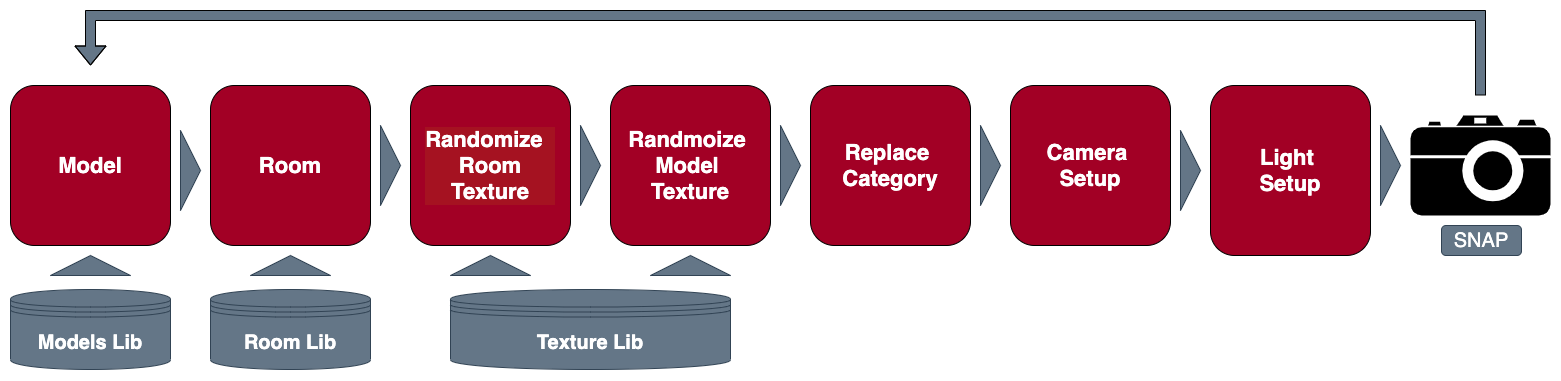
\includegraphics[width=\textwidth]{/Users/apple/OVGU/Thesis/code/3dReconstruction/report/images/concept/process}
    \caption[Overview of 3D-Scene Tool]{An overview of pipeline for image generation with different blocks and external libraries.
    Each block is discussed in sections mentioned in the figure.}
    \label{fig:pipeline process}
\end{figure}

\subsection{Furniture Models from Pix3D}\label{subsec:furniture-models-from-pix3d}
As discussed in \autoref{subsec:why-pix3d?}, we utilize 3D furniture models from Pix3D.
Pix3D provides 381 models for pieces of furniture with seven categories(Bed, Bookcase, Chair, Desk, Sofa, Table, Wardrobe).
Most of the models have default textures, while some do not.
These textures will be changed randomly within the pipeline.

\subsection{Scenes from SceneNet}\label{subsec:scenes-from-scenenet}
We utilize scenes provided by SceneNet~\cite{McCormac2017} for the rooms in our ersatz environments.
All the categories from Pix3D are also present in ShapeNet, which are used to fill the space in SceneNet.
The distribution of furniture matching the category of Pix3D in the scenes is as shown in \autoref{fig:distribution of scenes}.
The application modifies each scene for every snap we take for the dataset we create at random.

\begin{figure}[!ht]
    \resizebox{0.49\textwidth}{6cm}{%% Creator: Matplotlib, PGF backend
%%
%% To include the figure in your LaTeX document, write
%%   \input{<filename>.pgf}
%%
%% Make sure the required packages are loaded in your preamble
%%   \usepackage{pgf}
%%
%% Figures using additional raster images can only be included by \input if
%% they are in the same directory as the main LaTeX file. For loading figures
%% from other directories you can use the `import` package
%%   \usepackage{import}
%%
%% and then include the figures with
%%   \import{<path to file>}{<filename>.pgf}
%%
%% Matplotlib used the following preamble
%%   \usepackage{fontspec}
%%   \setmainfont{DejaVuSerif.ttf}[Path=\detokenize{/Users/apple/opt/anaconda3/envs/kaolin/lib/python3.7/site-packages/matplotlib/mpl-data/fonts/ttf/}]
%%   \setsansfont{DejaVuSans.ttf}[Path=\detokenize{/Users/apple/opt/anaconda3/envs/kaolin/lib/python3.7/site-packages/matplotlib/mpl-data/fonts/ttf/}]
%%   \setmonofont{DejaVuSansMono.ttf}[Path=\detokenize{/Users/apple/opt/anaconda3/envs/kaolin/lib/python3.7/site-packages/matplotlib/mpl-data/fonts/ttf/}]
%%
\begingroup%
\makeatletter%
\begin{pgfpicture}%
\pgfpathrectangle{\pgfpointorigin}{\pgfqpoint{5.433953in}{4.337596in}}%
\pgfusepath{use as bounding box, clip}%
\begin{pgfscope}%
\pgfsetbuttcap%
\pgfsetmiterjoin%
\definecolor{currentfill}{rgb}{1.000000,1.000000,1.000000}%
\pgfsetfillcolor{currentfill}%
\pgfsetlinewidth{0.000000pt}%
\definecolor{currentstroke}{rgb}{1.000000,1.000000,1.000000}%
\pgfsetstrokecolor{currentstroke}%
\pgfsetdash{}{0pt}%
\pgfpathmoveto{\pgfqpoint{0.000000in}{0.000000in}}%
\pgfpathlineto{\pgfqpoint{5.433953in}{0.000000in}}%
\pgfpathlineto{\pgfqpoint{5.433953in}{4.337596in}}%
\pgfpathlineto{\pgfqpoint{0.000000in}{4.337596in}}%
\pgfpathclose%
\pgfusepath{fill}%
\end{pgfscope}%
\begin{pgfscope}%
\pgfsetbuttcap%
\pgfsetmiterjoin%
\definecolor{currentfill}{rgb}{1.000000,1.000000,1.000000}%
\pgfsetfillcolor{currentfill}%
\pgfsetlinewidth{0.000000pt}%
\definecolor{currentstroke}{rgb}{0.000000,0.000000,0.000000}%
\pgfsetstrokecolor{currentstroke}%
\pgfsetstrokeopacity{0.000000}%
\pgfsetdash{}{0pt}%
\pgfpathmoveto{\pgfqpoint{0.373953in}{0.331635in}}%
\pgfpathlineto{\pgfqpoint{5.333953in}{0.331635in}}%
\pgfpathlineto{\pgfqpoint{5.333953in}{4.027635in}}%
\pgfpathlineto{\pgfqpoint{0.373953in}{4.027635in}}%
\pgfpathclose%
\pgfusepath{fill}%
\end{pgfscope}%
\begin{pgfscope}%
\pgfpathrectangle{\pgfqpoint{0.373953in}{0.331635in}}{\pgfqpoint{4.960000in}{3.696000in}}%
\pgfusepath{clip}%
\pgfsetbuttcap%
\pgfsetmiterjoin%
\definecolor{currentfill}{rgb}{0.000000,0.000000,1.000000}%
\pgfsetfillcolor{currentfill}%
\pgfsetlinewidth{0.000000pt}%
\definecolor{currentstroke}{rgb}{0.000000,0.000000,0.000000}%
\pgfsetstrokecolor{currentstroke}%
\pgfsetstrokeopacity{0.000000}%
\pgfsetdash{}{0pt}%
\pgfpathmoveto{\pgfqpoint{0.599407in}{0.331635in}}%
\pgfpathlineto{\pgfqpoint{1.548690in}{0.331635in}}%
\pgfpathlineto{\pgfqpoint{1.548690in}{2.571635in}}%
\pgfpathlineto{\pgfqpoint{0.599407in}{2.571635in}}%
\pgfpathclose%
\pgfusepath{fill}%
\end{pgfscope}%
\begin{pgfscope}%
\pgfpathrectangle{\pgfqpoint{0.373953in}{0.331635in}}{\pgfqpoint{4.960000in}{3.696000in}}%
\pgfusepath{clip}%
\pgfsetbuttcap%
\pgfsetmiterjoin%
\definecolor{currentfill}{rgb}{0.000000,0.000000,1.000000}%
\pgfsetfillcolor{currentfill}%
\pgfsetlinewidth{0.000000pt}%
\definecolor{currentstroke}{rgb}{0.000000,0.000000,0.000000}%
\pgfsetstrokecolor{currentstroke}%
\pgfsetstrokeopacity{0.000000}%
\pgfsetdash{}{0pt}%
\pgfpathmoveto{\pgfqpoint{1.786010in}{0.331635in}}%
\pgfpathlineto{\pgfqpoint{2.735293in}{0.331635in}}%
\pgfpathlineto{\pgfqpoint{2.735293in}{0.651635in}}%
\pgfpathlineto{\pgfqpoint{1.786010in}{0.651635in}}%
\pgfpathclose%
\pgfusepath{fill}%
\end{pgfscope}%
\begin{pgfscope}%
\pgfpathrectangle{\pgfqpoint{0.373953in}{0.331635in}}{\pgfqpoint{4.960000in}{3.696000in}}%
\pgfusepath{clip}%
\pgfsetbuttcap%
\pgfsetmiterjoin%
\definecolor{currentfill}{rgb}{0.000000,0.000000,1.000000}%
\pgfsetfillcolor{currentfill}%
\pgfsetlinewidth{0.000000pt}%
\definecolor{currentstroke}{rgb}{0.000000,0.000000,0.000000}%
\pgfsetstrokecolor{currentstroke}%
\pgfsetstrokeopacity{0.000000}%
\pgfsetdash{}{0pt}%
\pgfpathmoveto{\pgfqpoint{2.972613in}{0.331635in}}%
\pgfpathlineto{\pgfqpoint{3.921896in}{0.331635in}}%
\pgfpathlineto{\pgfqpoint{3.921896in}{3.851635in}}%
\pgfpathlineto{\pgfqpoint{2.972613in}{3.851635in}}%
\pgfpathclose%
\pgfusepath{fill}%
\end{pgfscope}%
\begin{pgfscope}%
\pgfpathrectangle{\pgfqpoint{0.373953in}{0.331635in}}{\pgfqpoint{4.960000in}{3.696000in}}%
\pgfusepath{clip}%
\pgfsetbuttcap%
\pgfsetmiterjoin%
\definecolor{currentfill}{rgb}{0.000000,0.000000,1.000000}%
\pgfsetfillcolor{currentfill}%
\pgfsetlinewidth{0.000000pt}%
\definecolor{currentstroke}{rgb}{0.000000,0.000000,0.000000}%
\pgfsetstrokecolor{currentstroke}%
\pgfsetstrokeopacity{0.000000}%
\pgfsetdash{}{0pt}%
\pgfpathmoveto{\pgfqpoint{4.159216in}{0.331635in}}%
\pgfpathlineto{\pgfqpoint{5.108498in}{0.331635in}}%
\pgfpathlineto{\pgfqpoint{5.108498in}{2.251635in}}%
\pgfpathlineto{\pgfqpoint{4.159216in}{2.251635in}}%
\pgfpathclose%
\pgfusepath{fill}%
\end{pgfscope}%
\begin{pgfscope}%
\pgfsetbuttcap%
\pgfsetroundjoin%
\definecolor{currentfill}{rgb}{0.000000,0.000000,0.000000}%
\pgfsetfillcolor{currentfill}%
\pgfsetlinewidth{0.803000pt}%
\definecolor{currentstroke}{rgb}{0.000000,0.000000,0.000000}%
\pgfsetstrokecolor{currentstroke}%
\pgfsetdash{}{0pt}%
\pgfsys@defobject{currentmarker}{\pgfqpoint{0.000000in}{-0.048611in}}{\pgfqpoint{0.000000in}{0.000000in}}{%
\pgfpathmoveto{\pgfqpoint{0.000000in}{0.000000in}}%
\pgfpathlineto{\pgfqpoint{0.000000in}{-0.048611in}}%
\pgfusepath{stroke,fill}%
}%
\begin{pgfscope}%
\pgfsys@transformshift{1.074049in}{0.331635in}%
\pgfsys@useobject{currentmarker}{}%
\end{pgfscope}%
\end{pgfscope}%
\begin{pgfscope}%
\definecolor{textcolor}{rgb}{0.000000,0.000000,0.000000}%
\pgfsetstrokecolor{textcolor}%
\pgfsetfillcolor{textcolor}%
\pgftext[x=1.074049in,y=0.234413in,,top]{\color{textcolor}\sffamily\fontsize{10.000000}{12.000000}\selectfont LivingRoom}%
\end{pgfscope}%
\begin{pgfscope}%
\pgfsetbuttcap%
\pgfsetroundjoin%
\definecolor{currentfill}{rgb}{0.000000,0.000000,0.000000}%
\pgfsetfillcolor{currentfill}%
\pgfsetlinewidth{0.803000pt}%
\definecolor{currentstroke}{rgb}{0.000000,0.000000,0.000000}%
\pgfsetstrokecolor{currentstroke}%
\pgfsetdash{}{0pt}%
\pgfsys@defobject{currentmarker}{\pgfqpoint{0.000000in}{-0.048611in}}{\pgfqpoint{0.000000in}{0.000000in}}{%
\pgfpathmoveto{\pgfqpoint{0.000000in}{0.000000in}}%
\pgfpathlineto{\pgfqpoint{0.000000in}{-0.048611in}}%
\pgfusepath{stroke,fill}%
}%
\begin{pgfscope}%
\pgfsys@transformshift{2.260651in}{0.331635in}%
\pgfsys@useobject{currentmarker}{}%
\end{pgfscope}%
\end{pgfscope}%
\begin{pgfscope}%
\definecolor{textcolor}{rgb}{0.000000,0.000000,0.000000}%
\pgfsetstrokecolor{textcolor}%
\pgfsetfillcolor{textcolor}%
\pgftext[x=2.260651in,y=0.234413in,,top]{\color{textcolor}\sffamily\fontsize{10.000000}{12.000000}\selectfont Kitchen}%
\end{pgfscope}%
\begin{pgfscope}%
\pgfsetbuttcap%
\pgfsetroundjoin%
\definecolor{currentfill}{rgb}{0.000000,0.000000,0.000000}%
\pgfsetfillcolor{currentfill}%
\pgfsetlinewidth{0.803000pt}%
\definecolor{currentstroke}{rgb}{0.000000,0.000000,0.000000}%
\pgfsetstrokecolor{currentstroke}%
\pgfsetdash{}{0pt}%
\pgfsys@defobject{currentmarker}{\pgfqpoint{0.000000in}{-0.048611in}}{\pgfqpoint{0.000000in}{0.000000in}}{%
\pgfpathmoveto{\pgfqpoint{0.000000in}{0.000000in}}%
\pgfpathlineto{\pgfqpoint{0.000000in}{-0.048611in}}%
\pgfusepath{stroke,fill}%
}%
\begin{pgfscope}%
\pgfsys@transformshift{3.447254in}{0.331635in}%
\pgfsys@useobject{currentmarker}{}%
\end{pgfscope}%
\end{pgfscope}%
\begin{pgfscope}%
\definecolor{textcolor}{rgb}{0.000000,0.000000,0.000000}%
\pgfsetstrokecolor{textcolor}%
\pgfsetfillcolor{textcolor}%
\pgftext[x=3.447254in,y=0.234413in,,top]{\color{textcolor}\sffamily\fontsize{10.000000}{12.000000}\selectfont Bedroom}%
\end{pgfscope}%
\begin{pgfscope}%
\pgfsetbuttcap%
\pgfsetroundjoin%
\definecolor{currentfill}{rgb}{0.000000,0.000000,0.000000}%
\pgfsetfillcolor{currentfill}%
\pgfsetlinewidth{0.803000pt}%
\definecolor{currentstroke}{rgb}{0.000000,0.000000,0.000000}%
\pgfsetstrokecolor{currentstroke}%
\pgfsetdash{}{0pt}%
\pgfsys@defobject{currentmarker}{\pgfqpoint{0.000000in}{-0.048611in}}{\pgfqpoint{0.000000in}{0.000000in}}{%
\pgfpathmoveto{\pgfqpoint{0.000000in}{0.000000in}}%
\pgfpathlineto{\pgfqpoint{0.000000in}{-0.048611in}}%
\pgfusepath{stroke,fill}%
}%
\begin{pgfscope}%
\pgfsys@transformshift{4.633857in}{0.331635in}%
\pgfsys@useobject{currentmarker}{}%
\end{pgfscope}%
\end{pgfscope}%
\begin{pgfscope}%
\definecolor{textcolor}{rgb}{0.000000,0.000000,0.000000}%
\pgfsetstrokecolor{textcolor}%
\pgfsetfillcolor{textcolor}%
\pgftext[x=4.633857in,y=0.234413in,,top]{\color{textcolor}\sffamily\fontsize{10.000000}{12.000000}\selectfont Office}%
\end{pgfscope}%
\begin{pgfscope}%
\pgfsetbuttcap%
\pgfsetroundjoin%
\definecolor{currentfill}{rgb}{0.000000,0.000000,0.000000}%
\pgfsetfillcolor{currentfill}%
\pgfsetlinewidth{0.803000pt}%
\definecolor{currentstroke}{rgb}{0.000000,0.000000,0.000000}%
\pgfsetstrokecolor{currentstroke}%
\pgfsetdash{}{0pt}%
\pgfsys@defobject{currentmarker}{\pgfqpoint{-0.048611in}{0.000000in}}{\pgfqpoint{-0.000000in}{0.000000in}}{%
\pgfpathmoveto{\pgfqpoint{-0.000000in}{0.000000in}}%
\pgfpathlineto{\pgfqpoint{-0.048611in}{0.000000in}}%
\pgfusepath{stroke,fill}%
}%
\begin{pgfscope}%
\pgfsys@transformshift{0.373953in}{0.331635in}%
\pgfsys@useobject{currentmarker}{}%
\end{pgfscope}%
\end{pgfscope}%
\begin{pgfscope}%
\definecolor{textcolor}{rgb}{0.000000,0.000000,0.000000}%
\pgfsetstrokecolor{textcolor}%
\pgfsetfillcolor{textcolor}%
\pgftext[x=0.188365in, y=0.278873in, left, base]{\color{textcolor}\sffamily\fontsize{10.000000}{12.000000}\selectfont 0}%
\end{pgfscope}%
\begin{pgfscope}%
\pgfsetbuttcap%
\pgfsetroundjoin%
\definecolor{currentfill}{rgb}{0.000000,0.000000,0.000000}%
\pgfsetfillcolor{currentfill}%
\pgfsetlinewidth{0.803000pt}%
\definecolor{currentstroke}{rgb}{0.000000,0.000000,0.000000}%
\pgfsetstrokecolor{currentstroke}%
\pgfsetdash{}{0pt}%
\pgfsys@defobject{currentmarker}{\pgfqpoint{-0.048611in}{0.000000in}}{\pgfqpoint{-0.000000in}{0.000000in}}{%
\pgfpathmoveto{\pgfqpoint{-0.000000in}{0.000000in}}%
\pgfpathlineto{\pgfqpoint{-0.048611in}{0.000000in}}%
\pgfusepath{stroke,fill}%
}%
\begin{pgfscope}%
\pgfsys@transformshift{0.373953in}{0.971635in}%
\pgfsys@useobject{currentmarker}{}%
\end{pgfscope}%
\end{pgfscope}%
\begin{pgfscope}%
\definecolor{textcolor}{rgb}{0.000000,0.000000,0.000000}%
\pgfsetstrokecolor{textcolor}%
\pgfsetfillcolor{textcolor}%
\pgftext[x=0.188365in, y=0.918873in, left, base]{\color{textcolor}\sffamily\fontsize{10.000000}{12.000000}\selectfont 2}%
\end{pgfscope}%
\begin{pgfscope}%
\pgfsetbuttcap%
\pgfsetroundjoin%
\definecolor{currentfill}{rgb}{0.000000,0.000000,0.000000}%
\pgfsetfillcolor{currentfill}%
\pgfsetlinewidth{0.803000pt}%
\definecolor{currentstroke}{rgb}{0.000000,0.000000,0.000000}%
\pgfsetstrokecolor{currentstroke}%
\pgfsetdash{}{0pt}%
\pgfsys@defobject{currentmarker}{\pgfqpoint{-0.048611in}{0.000000in}}{\pgfqpoint{-0.000000in}{0.000000in}}{%
\pgfpathmoveto{\pgfqpoint{-0.000000in}{0.000000in}}%
\pgfpathlineto{\pgfqpoint{-0.048611in}{0.000000in}}%
\pgfusepath{stroke,fill}%
}%
\begin{pgfscope}%
\pgfsys@transformshift{0.373953in}{1.611635in}%
\pgfsys@useobject{currentmarker}{}%
\end{pgfscope}%
\end{pgfscope}%
\begin{pgfscope}%
\definecolor{textcolor}{rgb}{0.000000,0.000000,0.000000}%
\pgfsetstrokecolor{textcolor}%
\pgfsetfillcolor{textcolor}%
\pgftext[x=0.188365in, y=1.558873in, left, base]{\color{textcolor}\sffamily\fontsize{10.000000}{12.000000}\selectfont 4}%
\end{pgfscope}%
\begin{pgfscope}%
\pgfsetbuttcap%
\pgfsetroundjoin%
\definecolor{currentfill}{rgb}{0.000000,0.000000,0.000000}%
\pgfsetfillcolor{currentfill}%
\pgfsetlinewidth{0.803000pt}%
\definecolor{currentstroke}{rgb}{0.000000,0.000000,0.000000}%
\pgfsetstrokecolor{currentstroke}%
\pgfsetdash{}{0pt}%
\pgfsys@defobject{currentmarker}{\pgfqpoint{-0.048611in}{0.000000in}}{\pgfqpoint{-0.000000in}{0.000000in}}{%
\pgfpathmoveto{\pgfqpoint{-0.000000in}{0.000000in}}%
\pgfpathlineto{\pgfqpoint{-0.048611in}{0.000000in}}%
\pgfusepath{stroke,fill}%
}%
\begin{pgfscope}%
\pgfsys@transformshift{0.373953in}{2.251635in}%
\pgfsys@useobject{currentmarker}{}%
\end{pgfscope}%
\end{pgfscope}%
\begin{pgfscope}%
\definecolor{textcolor}{rgb}{0.000000,0.000000,0.000000}%
\pgfsetstrokecolor{textcolor}%
\pgfsetfillcolor{textcolor}%
\pgftext[x=0.188365in, y=2.198873in, left, base]{\color{textcolor}\sffamily\fontsize{10.000000}{12.000000}\selectfont 6}%
\end{pgfscope}%
\begin{pgfscope}%
\pgfsetbuttcap%
\pgfsetroundjoin%
\definecolor{currentfill}{rgb}{0.000000,0.000000,0.000000}%
\pgfsetfillcolor{currentfill}%
\pgfsetlinewidth{0.803000pt}%
\definecolor{currentstroke}{rgb}{0.000000,0.000000,0.000000}%
\pgfsetstrokecolor{currentstroke}%
\pgfsetdash{}{0pt}%
\pgfsys@defobject{currentmarker}{\pgfqpoint{-0.048611in}{0.000000in}}{\pgfqpoint{-0.000000in}{0.000000in}}{%
\pgfpathmoveto{\pgfqpoint{-0.000000in}{0.000000in}}%
\pgfpathlineto{\pgfqpoint{-0.048611in}{0.000000in}}%
\pgfusepath{stroke,fill}%
}%
\begin{pgfscope}%
\pgfsys@transformshift{0.373953in}{2.891635in}%
\pgfsys@useobject{currentmarker}{}%
\end{pgfscope}%
\end{pgfscope}%
\begin{pgfscope}%
\definecolor{textcolor}{rgb}{0.000000,0.000000,0.000000}%
\pgfsetstrokecolor{textcolor}%
\pgfsetfillcolor{textcolor}%
\pgftext[x=0.188365in, y=2.838873in, left, base]{\color{textcolor}\sffamily\fontsize{10.000000}{12.000000}\selectfont 8}%
\end{pgfscope}%
\begin{pgfscope}%
\pgfsetbuttcap%
\pgfsetroundjoin%
\definecolor{currentfill}{rgb}{0.000000,0.000000,0.000000}%
\pgfsetfillcolor{currentfill}%
\pgfsetlinewidth{0.803000pt}%
\definecolor{currentstroke}{rgb}{0.000000,0.000000,0.000000}%
\pgfsetstrokecolor{currentstroke}%
\pgfsetdash{}{0pt}%
\pgfsys@defobject{currentmarker}{\pgfqpoint{-0.048611in}{0.000000in}}{\pgfqpoint{-0.000000in}{0.000000in}}{%
\pgfpathmoveto{\pgfqpoint{-0.000000in}{0.000000in}}%
\pgfpathlineto{\pgfqpoint{-0.048611in}{0.000000in}}%
\pgfusepath{stroke,fill}%
}%
\begin{pgfscope}%
\pgfsys@transformshift{0.373953in}{3.531635in}%
\pgfsys@useobject{currentmarker}{}%
\end{pgfscope}%
\end{pgfscope}%
\begin{pgfscope}%
\definecolor{textcolor}{rgb}{0.000000,0.000000,0.000000}%
\pgfsetstrokecolor{textcolor}%
\pgfsetfillcolor{textcolor}%
\pgftext[x=0.100000in, y=3.478873in, left, base]{\color{textcolor}\sffamily\fontsize{10.000000}{12.000000}\selectfont 10}%
\end{pgfscope}%
\begin{pgfscope}%
\pgfsetrectcap%
\pgfsetmiterjoin%
\pgfsetlinewidth{0.803000pt}%
\definecolor{currentstroke}{rgb}{0.000000,0.000000,0.000000}%
\pgfsetstrokecolor{currentstroke}%
\pgfsetdash{}{0pt}%
\pgfpathmoveto{\pgfqpoint{0.373953in}{0.331635in}}%
\pgfpathlineto{\pgfqpoint{0.373953in}{4.027635in}}%
\pgfusepath{stroke}%
\end{pgfscope}%
\begin{pgfscope}%
\pgfsetrectcap%
\pgfsetmiterjoin%
\pgfsetlinewidth{0.803000pt}%
\definecolor{currentstroke}{rgb}{0.000000,0.000000,0.000000}%
\pgfsetstrokecolor{currentstroke}%
\pgfsetdash{}{0pt}%
\pgfpathmoveto{\pgfqpoint{5.333953in}{0.331635in}}%
\pgfpathlineto{\pgfqpoint{5.333953in}{4.027635in}}%
\pgfusepath{stroke}%
\end{pgfscope}%
\begin{pgfscope}%
\pgfsetrectcap%
\pgfsetmiterjoin%
\pgfsetlinewidth{0.803000pt}%
\definecolor{currentstroke}{rgb}{0.000000,0.000000,0.000000}%
\pgfsetstrokecolor{currentstroke}%
\pgfsetdash{}{0pt}%
\pgfpathmoveto{\pgfqpoint{0.373953in}{0.331635in}}%
\pgfpathlineto{\pgfqpoint{5.333953in}{0.331635in}}%
\pgfusepath{stroke}%
\end{pgfscope}%
\begin{pgfscope}%
\pgfsetrectcap%
\pgfsetmiterjoin%
\pgfsetlinewidth{0.803000pt}%
\definecolor{currentstroke}{rgb}{0.000000,0.000000,0.000000}%
\pgfsetstrokecolor{currentstroke}%
\pgfsetdash{}{0pt}%
\pgfpathmoveto{\pgfqpoint{0.373953in}{4.027635in}}%
\pgfpathlineto{\pgfqpoint{5.333953in}{4.027635in}}%
\pgfusepath{stroke}%
\end{pgfscope}%
\begin{pgfscope}%
\definecolor{textcolor}{rgb}{0.000000,0.000000,0.000000}%
\pgfsetstrokecolor{textcolor}%
\pgfsetfillcolor{textcolor}%
\pgftext[x=2.853953in,y=4.110968in,,base]{\color{textcolor}\sffamily\fontsize{12.000000}{14.400000}\selectfont Type of scenes}%
\end{pgfscope}%
\end{pgfpicture}%
\makeatother%
\endgroup%
}
    \resizebox{0.49\textwidth}{6cm}{%% Creator: Matplotlib, PGF backend
%%
%% To include the figure in your LaTeX document, write
%%   \input{<filename>.pgf}
%%
%% Make sure the required packages are loaded in your preamble
%%   \usepackage{pgf}
%%
%% Figures using additional raster images can only be included by \input if
%% they are in the same directory as the main LaTeX file. For loading figures
%% from other directories you can use the `import` package
%%   \usepackage{import}
%%
%% and then include the figures with
%%   \import{<path to file>}{<filename>.pgf}
%%
%% Matplotlib used the following preamble
%%   \usepackage{fontspec}
%%   \setmainfont{DejaVuSerif.ttf}[Path=\detokenize{/Users/apple/opt/anaconda3/envs/kaolin/lib/python3.7/site-packages/matplotlib/mpl-data/fonts/ttf/}]
%%   \setsansfont{DejaVuSans.ttf}[Path=\detokenize{/Users/apple/opt/anaconda3/envs/kaolin/lib/python3.7/site-packages/matplotlib/mpl-data/fonts/ttf/}]
%%   \setmonofont{DejaVuSansMono.ttf}[Path=\detokenize{/Users/apple/opt/anaconda3/envs/kaolin/lib/python3.7/site-packages/matplotlib/mpl-data/fonts/ttf/}]
%%
\begingroup%
\makeatletter%
\begin{pgfpicture}%
\pgfpathrectangle{\pgfpointorigin}{\pgfqpoint{5.522318in}{4.337596in}}%
\pgfusepath{use as bounding box, clip}%
\begin{pgfscope}%
\pgfsetbuttcap%
\pgfsetmiterjoin%
\definecolor{currentfill}{rgb}{1.000000,1.000000,1.000000}%
\pgfsetfillcolor{currentfill}%
\pgfsetlinewidth{0.000000pt}%
\definecolor{currentstroke}{rgb}{1.000000,1.000000,1.000000}%
\pgfsetstrokecolor{currentstroke}%
\pgfsetdash{}{0pt}%
\pgfpathmoveto{\pgfqpoint{0.000000in}{0.000000in}}%
\pgfpathlineto{\pgfqpoint{5.522318in}{0.000000in}}%
\pgfpathlineto{\pgfqpoint{5.522318in}{4.337596in}}%
\pgfpathlineto{\pgfqpoint{0.000000in}{4.337596in}}%
\pgfpathclose%
\pgfusepath{fill}%
\end{pgfscope}%
\begin{pgfscope}%
\pgfsetbuttcap%
\pgfsetmiterjoin%
\definecolor{currentfill}{rgb}{1.000000,1.000000,1.000000}%
\pgfsetfillcolor{currentfill}%
\pgfsetlinewidth{0.000000pt}%
\definecolor{currentstroke}{rgb}{0.000000,0.000000,0.000000}%
\pgfsetstrokecolor{currentstroke}%
\pgfsetstrokeopacity{0.000000}%
\pgfsetdash{}{0pt}%
\pgfpathmoveto{\pgfqpoint{0.462318in}{0.331635in}}%
\pgfpathlineto{\pgfqpoint{5.422318in}{0.331635in}}%
\pgfpathlineto{\pgfqpoint{5.422318in}{4.027635in}}%
\pgfpathlineto{\pgfqpoint{0.462318in}{4.027635in}}%
\pgfpathclose%
\pgfusepath{fill}%
\end{pgfscope}%
\begin{pgfscope}%
\pgfpathrectangle{\pgfqpoint{0.462318in}{0.331635in}}{\pgfqpoint{4.960000in}{3.696000in}}%
\pgfusepath{clip}%
\pgfsetbuttcap%
\pgfsetmiterjoin%
\definecolor{currentfill}{rgb}{0.121569,0.466667,0.705882}%
\pgfsetfillcolor{currentfill}%
\pgfsetlinewidth{0.000000pt}%
\definecolor{currentstroke}{rgb}{0.000000,0.000000,0.000000}%
\pgfsetstrokecolor{currentstroke}%
\pgfsetstrokeopacity{0.000000}%
\pgfsetdash{}{0pt}%
\pgfpathmoveto{\pgfqpoint{0.687773in}{0.331635in}}%
\pgfpathlineto{\pgfqpoint{1.218254in}{0.331635in}}%
\pgfpathlineto{\pgfqpoint{1.218254in}{3.851635in}}%
\pgfpathlineto{\pgfqpoint{0.687773in}{3.851635in}}%
\pgfpathclose%
\pgfusepath{fill}%
\end{pgfscope}%
\begin{pgfscope}%
\pgfpathrectangle{\pgfqpoint{0.462318in}{0.331635in}}{\pgfqpoint{4.960000in}{3.696000in}}%
\pgfusepath{clip}%
\pgfsetbuttcap%
\pgfsetmiterjoin%
\definecolor{currentfill}{rgb}{0.121569,0.466667,0.705882}%
\pgfsetfillcolor{currentfill}%
\pgfsetlinewidth{0.000000pt}%
\definecolor{currentstroke}{rgb}{0.000000,0.000000,0.000000}%
\pgfsetstrokecolor{currentstroke}%
\pgfsetstrokeopacity{0.000000}%
\pgfsetdash{}{0pt}%
\pgfpathmoveto{\pgfqpoint{1.350874in}{0.331635in}}%
\pgfpathlineto{\pgfqpoint{1.881356in}{0.331635in}}%
\pgfpathlineto{\pgfqpoint{1.881356in}{1.079246in}}%
\pgfpathlineto{\pgfqpoint{1.350874in}{1.079246in}}%
\pgfpathclose%
\pgfusepath{fill}%
\end{pgfscope}%
\begin{pgfscope}%
\pgfpathrectangle{\pgfqpoint{0.462318in}{0.331635in}}{\pgfqpoint{4.960000in}{3.696000in}}%
\pgfusepath{clip}%
\pgfsetbuttcap%
\pgfsetmiterjoin%
\definecolor{currentfill}{rgb}{0.121569,0.466667,0.705882}%
\pgfsetfillcolor{currentfill}%
\pgfsetlinewidth{0.000000pt}%
\definecolor{currentstroke}{rgb}{0.000000,0.000000,0.000000}%
\pgfsetstrokecolor{currentstroke}%
\pgfsetstrokeopacity{0.000000}%
\pgfsetdash{}{0pt}%
\pgfpathmoveto{\pgfqpoint{2.013976in}{0.331635in}}%
\pgfpathlineto{\pgfqpoint{2.544457in}{0.331635in}}%
\pgfpathlineto{\pgfqpoint{2.544457in}{1.484201in}}%
\pgfpathlineto{\pgfqpoint{2.013976in}{1.484201in}}%
\pgfpathclose%
\pgfusepath{fill}%
\end{pgfscope}%
\begin{pgfscope}%
\pgfpathrectangle{\pgfqpoint{0.462318in}{0.331635in}}{\pgfqpoint{4.960000in}{3.696000in}}%
\pgfusepath{clip}%
\pgfsetbuttcap%
\pgfsetmiterjoin%
\definecolor{currentfill}{rgb}{0.121569,0.466667,0.705882}%
\pgfsetfillcolor{currentfill}%
\pgfsetlinewidth{0.000000pt}%
\definecolor{currentstroke}{rgb}{0.000000,0.000000,0.000000}%
\pgfsetstrokecolor{currentstroke}%
\pgfsetstrokeopacity{0.000000}%
\pgfsetdash{}{0pt}%
\pgfpathmoveto{\pgfqpoint{2.677078in}{0.331635in}}%
\pgfpathlineto{\pgfqpoint{3.207559in}{0.331635in}}%
\pgfpathlineto{\pgfqpoint{3.207559in}{0.954644in}}%
\pgfpathlineto{\pgfqpoint{2.677078in}{0.954644in}}%
\pgfpathclose%
\pgfusepath{fill}%
\end{pgfscope}%
\begin{pgfscope}%
\pgfpathrectangle{\pgfqpoint{0.462318in}{0.331635in}}{\pgfqpoint{4.960000in}{3.696000in}}%
\pgfusepath{clip}%
\pgfsetbuttcap%
\pgfsetmiterjoin%
\definecolor{currentfill}{rgb}{0.121569,0.466667,0.705882}%
\pgfsetfillcolor{currentfill}%
\pgfsetlinewidth{0.000000pt}%
\definecolor{currentstroke}{rgb}{0.000000,0.000000,0.000000}%
\pgfsetstrokecolor{currentstroke}%
\pgfsetstrokeopacity{0.000000}%
\pgfsetdash{}{0pt}%
\pgfpathmoveto{\pgfqpoint{3.340179in}{0.331635in}}%
\pgfpathlineto{\pgfqpoint{3.870660in}{0.331635in}}%
\pgfpathlineto{\pgfqpoint{3.870660in}{1.048095in}}%
\pgfpathlineto{\pgfqpoint{3.340179in}{1.048095in}}%
\pgfpathclose%
\pgfusepath{fill}%
\end{pgfscope}%
\begin{pgfscope}%
\pgfpathrectangle{\pgfqpoint{0.462318in}{0.331635in}}{\pgfqpoint{4.960000in}{3.696000in}}%
\pgfusepath{clip}%
\pgfsetbuttcap%
\pgfsetmiterjoin%
\definecolor{currentfill}{rgb}{0.121569,0.466667,0.705882}%
\pgfsetfillcolor{currentfill}%
\pgfsetlinewidth{0.000000pt}%
\definecolor{currentstroke}{rgb}{0.000000,0.000000,0.000000}%
\pgfsetstrokecolor{currentstroke}%
\pgfsetstrokeopacity{0.000000}%
\pgfsetdash{}{0pt}%
\pgfpathmoveto{\pgfqpoint{4.003281in}{0.331635in}}%
\pgfpathlineto{\pgfqpoint{4.533762in}{0.331635in}}%
\pgfpathlineto{\pgfqpoint{4.533762in}{1.390750in}}%
\pgfpathlineto{\pgfqpoint{4.003281in}{1.390750in}}%
\pgfpathclose%
\pgfusepath{fill}%
\end{pgfscope}%
\begin{pgfscope}%
\pgfpathrectangle{\pgfqpoint{0.462318in}{0.331635in}}{\pgfqpoint{4.960000in}{3.696000in}}%
\pgfusepath{clip}%
\pgfsetbuttcap%
\pgfsetmiterjoin%
\definecolor{currentfill}{rgb}{0.121569,0.466667,0.705882}%
\pgfsetfillcolor{currentfill}%
\pgfsetlinewidth{0.000000pt}%
\definecolor{currentstroke}{rgb}{0.000000,0.000000,0.000000}%
\pgfsetstrokecolor{currentstroke}%
\pgfsetstrokeopacity{0.000000}%
\pgfsetdash{}{0pt}%
\pgfpathmoveto{\pgfqpoint{4.666382in}{0.331635in}}%
\pgfpathlineto{\pgfqpoint{5.196864in}{0.331635in}}%
\pgfpathlineto{\pgfqpoint{5.196864in}{0.674290in}}%
\pgfpathlineto{\pgfqpoint{4.666382in}{0.674290in}}%
\pgfpathclose%
\pgfusepath{fill}%
\end{pgfscope}%
\begin{pgfscope}%
\pgfsetbuttcap%
\pgfsetroundjoin%
\definecolor{currentfill}{rgb}{0.000000,0.000000,0.000000}%
\pgfsetfillcolor{currentfill}%
\pgfsetlinewidth{0.803000pt}%
\definecolor{currentstroke}{rgb}{0.000000,0.000000,0.000000}%
\pgfsetstrokecolor{currentstroke}%
\pgfsetdash{}{0pt}%
\pgfsys@defobject{currentmarker}{\pgfqpoint{0.000000in}{-0.048611in}}{\pgfqpoint{0.000000in}{0.000000in}}{%
\pgfpathmoveto{\pgfqpoint{0.000000in}{0.000000in}}%
\pgfpathlineto{\pgfqpoint{0.000000in}{-0.048611in}}%
\pgfusepath{stroke,fill}%
}%
\begin{pgfscope}%
\pgfsys@transformshift{0.953013in}{0.331635in}%
\pgfsys@useobject{currentmarker}{}%
\end{pgfscope}%
\end{pgfscope}%
\begin{pgfscope}%
\definecolor{textcolor}{rgb}{0.000000,0.000000,0.000000}%
\pgfsetstrokecolor{textcolor}%
\pgfsetfillcolor{textcolor}%
\pgftext[x=0.953013in,y=0.234413in,,top]{\color{textcolor}\sffamily\fontsize{10.000000}{12.000000}\selectfont chair}%
\end{pgfscope}%
\begin{pgfscope}%
\pgfsetbuttcap%
\pgfsetroundjoin%
\definecolor{currentfill}{rgb}{0.000000,0.000000,0.000000}%
\pgfsetfillcolor{currentfill}%
\pgfsetlinewidth{0.803000pt}%
\definecolor{currentstroke}{rgb}{0.000000,0.000000,0.000000}%
\pgfsetstrokecolor{currentstroke}%
\pgfsetdash{}{0pt}%
\pgfsys@defobject{currentmarker}{\pgfqpoint{0.000000in}{-0.048611in}}{\pgfqpoint{0.000000in}{0.000000in}}{%
\pgfpathmoveto{\pgfqpoint{0.000000in}{0.000000in}}%
\pgfpathlineto{\pgfqpoint{0.000000in}{-0.048611in}}%
\pgfusepath{stroke,fill}%
}%
\begin{pgfscope}%
\pgfsys@transformshift{1.616115in}{0.331635in}%
\pgfsys@useobject{currentmarker}{}%
\end{pgfscope}%
\end{pgfscope}%
\begin{pgfscope}%
\definecolor{textcolor}{rgb}{0.000000,0.000000,0.000000}%
\pgfsetstrokecolor{textcolor}%
\pgfsetfillcolor{textcolor}%
\pgftext[x=1.616115in,y=0.234413in,,top]{\color{textcolor}\sffamily\fontsize{10.000000}{12.000000}\selectfont bed}%
\end{pgfscope}%
\begin{pgfscope}%
\pgfsetbuttcap%
\pgfsetroundjoin%
\definecolor{currentfill}{rgb}{0.000000,0.000000,0.000000}%
\pgfsetfillcolor{currentfill}%
\pgfsetlinewidth{0.803000pt}%
\definecolor{currentstroke}{rgb}{0.000000,0.000000,0.000000}%
\pgfsetstrokecolor{currentstroke}%
\pgfsetdash{}{0pt}%
\pgfsys@defobject{currentmarker}{\pgfqpoint{0.000000in}{-0.048611in}}{\pgfqpoint{0.000000in}{0.000000in}}{%
\pgfpathmoveto{\pgfqpoint{0.000000in}{0.000000in}}%
\pgfpathlineto{\pgfqpoint{0.000000in}{-0.048611in}}%
\pgfusepath{stroke,fill}%
}%
\begin{pgfscope}%
\pgfsys@transformshift{2.279217in}{0.331635in}%
\pgfsys@useobject{currentmarker}{}%
\end{pgfscope}%
\end{pgfscope}%
\begin{pgfscope}%
\definecolor{textcolor}{rgb}{0.000000,0.000000,0.000000}%
\pgfsetstrokecolor{textcolor}%
\pgfsetfillcolor{textcolor}%
\pgftext[x=2.279217in,y=0.234413in,,top]{\color{textcolor}\sffamily\fontsize{10.000000}{12.000000}\selectfont desk}%
\end{pgfscope}%
\begin{pgfscope}%
\pgfsetbuttcap%
\pgfsetroundjoin%
\definecolor{currentfill}{rgb}{0.000000,0.000000,0.000000}%
\pgfsetfillcolor{currentfill}%
\pgfsetlinewidth{0.803000pt}%
\definecolor{currentstroke}{rgb}{0.000000,0.000000,0.000000}%
\pgfsetstrokecolor{currentstroke}%
\pgfsetdash{}{0pt}%
\pgfsys@defobject{currentmarker}{\pgfqpoint{0.000000in}{-0.048611in}}{\pgfqpoint{0.000000in}{0.000000in}}{%
\pgfpathmoveto{\pgfqpoint{0.000000in}{0.000000in}}%
\pgfpathlineto{\pgfqpoint{0.000000in}{-0.048611in}}%
\pgfusepath{stroke,fill}%
}%
\begin{pgfscope}%
\pgfsys@transformshift{2.942318in}{0.331635in}%
\pgfsys@useobject{currentmarker}{}%
\end{pgfscope}%
\end{pgfscope}%
\begin{pgfscope}%
\definecolor{textcolor}{rgb}{0.000000,0.000000,0.000000}%
\pgfsetstrokecolor{textcolor}%
\pgfsetfillcolor{textcolor}%
\pgftext[x=2.942318in,y=0.234413in,,top]{\color{textcolor}\sffamily\fontsize{10.000000}{12.000000}\selectfont bookcase}%
\end{pgfscope}%
\begin{pgfscope}%
\pgfsetbuttcap%
\pgfsetroundjoin%
\definecolor{currentfill}{rgb}{0.000000,0.000000,0.000000}%
\pgfsetfillcolor{currentfill}%
\pgfsetlinewidth{0.803000pt}%
\definecolor{currentstroke}{rgb}{0.000000,0.000000,0.000000}%
\pgfsetstrokecolor{currentstroke}%
\pgfsetdash{}{0pt}%
\pgfsys@defobject{currentmarker}{\pgfqpoint{0.000000in}{-0.048611in}}{\pgfqpoint{0.000000in}{0.000000in}}{%
\pgfpathmoveto{\pgfqpoint{0.000000in}{0.000000in}}%
\pgfpathlineto{\pgfqpoint{0.000000in}{-0.048611in}}%
\pgfusepath{stroke,fill}%
}%
\begin{pgfscope}%
\pgfsys@transformshift{3.605420in}{0.331635in}%
\pgfsys@useobject{currentmarker}{}%
\end{pgfscope}%
\end{pgfscope}%
\begin{pgfscope}%
\definecolor{textcolor}{rgb}{0.000000,0.000000,0.000000}%
\pgfsetstrokecolor{textcolor}%
\pgfsetfillcolor{textcolor}%
\pgftext[x=3.605420in,y=0.234413in,,top]{\color{textcolor}\sffamily\fontsize{10.000000}{12.000000}\selectfont sofa}%
\end{pgfscope}%
\begin{pgfscope}%
\pgfsetbuttcap%
\pgfsetroundjoin%
\definecolor{currentfill}{rgb}{0.000000,0.000000,0.000000}%
\pgfsetfillcolor{currentfill}%
\pgfsetlinewidth{0.803000pt}%
\definecolor{currentstroke}{rgb}{0.000000,0.000000,0.000000}%
\pgfsetstrokecolor{currentstroke}%
\pgfsetdash{}{0pt}%
\pgfsys@defobject{currentmarker}{\pgfqpoint{0.000000in}{-0.048611in}}{\pgfqpoint{0.000000in}{0.000000in}}{%
\pgfpathmoveto{\pgfqpoint{0.000000in}{0.000000in}}%
\pgfpathlineto{\pgfqpoint{0.000000in}{-0.048611in}}%
\pgfusepath{stroke,fill}%
}%
\begin{pgfscope}%
\pgfsys@transformshift{4.268521in}{0.331635in}%
\pgfsys@useobject{currentmarker}{}%
\end{pgfscope}%
\end{pgfscope}%
\begin{pgfscope}%
\definecolor{textcolor}{rgb}{0.000000,0.000000,0.000000}%
\pgfsetstrokecolor{textcolor}%
\pgfsetfillcolor{textcolor}%
\pgftext[x=4.268521in,y=0.234413in,,top]{\color{textcolor}\sffamily\fontsize{10.000000}{12.000000}\selectfont table}%
\end{pgfscope}%
\begin{pgfscope}%
\pgfsetbuttcap%
\pgfsetroundjoin%
\definecolor{currentfill}{rgb}{0.000000,0.000000,0.000000}%
\pgfsetfillcolor{currentfill}%
\pgfsetlinewidth{0.803000pt}%
\definecolor{currentstroke}{rgb}{0.000000,0.000000,0.000000}%
\pgfsetstrokecolor{currentstroke}%
\pgfsetdash{}{0pt}%
\pgfsys@defobject{currentmarker}{\pgfqpoint{0.000000in}{-0.048611in}}{\pgfqpoint{0.000000in}{0.000000in}}{%
\pgfpathmoveto{\pgfqpoint{0.000000in}{0.000000in}}%
\pgfpathlineto{\pgfqpoint{0.000000in}{-0.048611in}}%
\pgfusepath{stroke,fill}%
}%
\begin{pgfscope}%
\pgfsys@transformshift{4.931623in}{0.331635in}%
\pgfsys@useobject{currentmarker}{}%
\end{pgfscope}%
\end{pgfscope}%
\begin{pgfscope}%
\definecolor{textcolor}{rgb}{0.000000,0.000000,0.000000}%
\pgfsetstrokecolor{textcolor}%
\pgfsetfillcolor{textcolor}%
\pgftext[x=4.931623in,y=0.234413in,,top]{\color{textcolor}\sffamily\fontsize{10.000000}{12.000000}\selectfont wardrobe}%
\end{pgfscope}%
\begin{pgfscope}%
\pgfsetbuttcap%
\pgfsetroundjoin%
\definecolor{currentfill}{rgb}{0.000000,0.000000,0.000000}%
\pgfsetfillcolor{currentfill}%
\pgfsetlinewidth{0.803000pt}%
\definecolor{currentstroke}{rgb}{0.000000,0.000000,0.000000}%
\pgfsetstrokecolor{currentstroke}%
\pgfsetdash{}{0pt}%
\pgfsys@defobject{currentmarker}{\pgfqpoint{-0.048611in}{0.000000in}}{\pgfqpoint{-0.000000in}{0.000000in}}{%
\pgfpathmoveto{\pgfqpoint{-0.000000in}{0.000000in}}%
\pgfpathlineto{\pgfqpoint{-0.048611in}{0.000000in}}%
\pgfusepath{stroke,fill}%
}%
\begin{pgfscope}%
\pgfsys@transformshift{0.462318in}{0.331635in}%
\pgfsys@useobject{currentmarker}{}%
\end{pgfscope}%
\end{pgfscope}%
\begin{pgfscope}%
\definecolor{textcolor}{rgb}{0.000000,0.000000,0.000000}%
\pgfsetstrokecolor{textcolor}%
\pgfsetfillcolor{textcolor}%
\pgftext[x=0.276731in, y=0.278873in, left, base]{\color{textcolor}\sffamily\fontsize{10.000000}{12.000000}\selectfont 0}%
\end{pgfscope}%
\begin{pgfscope}%
\pgfsetbuttcap%
\pgfsetroundjoin%
\definecolor{currentfill}{rgb}{0.000000,0.000000,0.000000}%
\pgfsetfillcolor{currentfill}%
\pgfsetlinewidth{0.803000pt}%
\definecolor{currentstroke}{rgb}{0.000000,0.000000,0.000000}%
\pgfsetstrokecolor{currentstroke}%
\pgfsetdash{}{0pt}%
\pgfsys@defobject{currentmarker}{\pgfqpoint{-0.048611in}{0.000000in}}{\pgfqpoint{-0.000000in}{0.000000in}}{%
\pgfpathmoveto{\pgfqpoint{-0.000000in}{0.000000in}}%
\pgfpathlineto{\pgfqpoint{-0.048611in}{0.000000in}}%
\pgfusepath{stroke,fill}%
}%
\begin{pgfscope}%
\pgfsys@transformshift{0.462318in}{0.954644in}%
\pgfsys@useobject{currentmarker}{}%
\end{pgfscope}%
\end{pgfscope}%
\begin{pgfscope}%
\definecolor{textcolor}{rgb}{0.000000,0.000000,0.000000}%
\pgfsetstrokecolor{textcolor}%
\pgfsetfillcolor{textcolor}%
\pgftext[x=0.188365in, y=0.901882in, left, base]{\color{textcolor}\sffamily\fontsize{10.000000}{12.000000}\selectfont 20}%
\end{pgfscope}%
\begin{pgfscope}%
\pgfsetbuttcap%
\pgfsetroundjoin%
\definecolor{currentfill}{rgb}{0.000000,0.000000,0.000000}%
\pgfsetfillcolor{currentfill}%
\pgfsetlinewidth{0.803000pt}%
\definecolor{currentstroke}{rgb}{0.000000,0.000000,0.000000}%
\pgfsetstrokecolor{currentstroke}%
\pgfsetdash{}{0pt}%
\pgfsys@defobject{currentmarker}{\pgfqpoint{-0.048611in}{0.000000in}}{\pgfqpoint{-0.000000in}{0.000000in}}{%
\pgfpathmoveto{\pgfqpoint{-0.000000in}{0.000000in}}%
\pgfpathlineto{\pgfqpoint{-0.048611in}{0.000000in}}%
\pgfusepath{stroke,fill}%
}%
\begin{pgfscope}%
\pgfsys@transformshift{0.462318in}{1.577653in}%
\pgfsys@useobject{currentmarker}{}%
\end{pgfscope}%
\end{pgfscope}%
\begin{pgfscope}%
\definecolor{textcolor}{rgb}{0.000000,0.000000,0.000000}%
\pgfsetstrokecolor{textcolor}%
\pgfsetfillcolor{textcolor}%
\pgftext[x=0.188365in, y=1.524891in, left, base]{\color{textcolor}\sffamily\fontsize{10.000000}{12.000000}\selectfont 40}%
\end{pgfscope}%
\begin{pgfscope}%
\pgfsetbuttcap%
\pgfsetroundjoin%
\definecolor{currentfill}{rgb}{0.000000,0.000000,0.000000}%
\pgfsetfillcolor{currentfill}%
\pgfsetlinewidth{0.803000pt}%
\definecolor{currentstroke}{rgb}{0.000000,0.000000,0.000000}%
\pgfsetstrokecolor{currentstroke}%
\pgfsetdash{}{0pt}%
\pgfsys@defobject{currentmarker}{\pgfqpoint{-0.048611in}{0.000000in}}{\pgfqpoint{-0.000000in}{0.000000in}}{%
\pgfpathmoveto{\pgfqpoint{-0.000000in}{0.000000in}}%
\pgfpathlineto{\pgfqpoint{-0.048611in}{0.000000in}}%
\pgfusepath{stroke,fill}%
}%
\begin{pgfscope}%
\pgfsys@transformshift{0.462318in}{2.200662in}%
\pgfsys@useobject{currentmarker}{}%
\end{pgfscope}%
\end{pgfscope}%
\begin{pgfscope}%
\definecolor{textcolor}{rgb}{0.000000,0.000000,0.000000}%
\pgfsetstrokecolor{textcolor}%
\pgfsetfillcolor{textcolor}%
\pgftext[x=0.188365in, y=2.147900in, left, base]{\color{textcolor}\sffamily\fontsize{10.000000}{12.000000}\selectfont 60}%
\end{pgfscope}%
\begin{pgfscope}%
\pgfsetbuttcap%
\pgfsetroundjoin%
\definecolor{currentfill}{rgb}{0.000000,0.000000,0.000000}%
\pgfsetfillcolor{currentfill}%
\pgfsetlinewidth{0.803000pt}%
\definecolor{currentstroke}{rgb}{0.000000,0.000000,0.000000}%
\pgfsetstrokecolor{currentstroke}%
\pgfsetdash{}{0pt}%
\pgfsys@defobject{currentmarker}{\pgfqpoint{-0.048611in}{0.000000in}}{\pgfqpoint{-0.000000in}{0.000000in}}{%
\pgfpathmoveto{\pgfqpoint{-0.000000in}{0.000000in}}%
\pgfpathlineto{\pgfqpoint{-0.048611in}{0.000000in}}%
\pgfusepath{stroke,fill}%
}%
\begin{pgfscope}%
\pgfsys@transformshift{0.462318in}{2.823670in}%
\pgfsys@useobject{currentmarker}{}%
\end{pgfscope}%
\end{pgfscope}%
\begin{pgfscope}%
\definecolor{textcolor}{rgb}{0.000000,0.000000,0.000000}%
\pgfsetstrokecolor{textcolor}%
\pgfsetfillcolor{textcolor}%
\pgftext[x=0.188365in, y=2.770909in, left, base]{\color{textcolor}\sffamily\fontsize{10.000000}{12.000000}\selectfont 80}%
\end{pgfscope}%
\begin{pgfscope}%
\pgfsetbuttcap%
\pgfsetroundjoin%
\definecolor{currentfill}{rgb}{0.000000,0.000000,0.000000}%
\pgfsetfillcolor{currentfill}%
\pgfsetlinewidth{0.803000pt}%
\definecolor{currentstroke}{rgb}{0.000000,0.000000,0.000000}%
\pgfsetstrokecolor{currentstroke}%
\pgfsetdash{}{0pt}%
\pgfsys@defobject{currentmarker}{\pgfqpoint{-0.048611in}{0.000000in}}{\pgfqpoint{-0.000000in}{0.000000in}}{%
\pgfpathmoveto{\pgfqpoint{-0.000000in}{0.000000in}}%
\pgfpathlineto{\pgfqpoint{-0.048611in}{0.000000in}}%
\pgfusepath{stroke,fill}%
}%
\begin{pgfscope}%
\pgfsys@transformshift{0.462318in}{3.446679in}%
\pgfsys@useobject{currentmarker}{}%
\end{pgfscope}%
\end{pgfscope}%
\begin{pgfscope}%
\definecolor{textcolor}{rgb}{0.000000,0.000000,0.000000}%
\pgfsetstrokecolor{textcolor}%
\pgfsetfillcolor{textcolor}%
\pgftext[x=0.100000in, y=3.393918in, left, base]{\color{textcolor}\sffamily\fontsize{10.000000}{12.000000}\selectfont 100}%
\end{pgfscope}%
\begin{pgfscope}%
\pgfsetrectcap%
\pgfsetmiterjoin%
\pgfsetlinewidth{0.803000pt}%
\definecolor{currentstroke}{rgb}{0.000000,0.000000,0.000000}%
\pgfsetstrokecolor{currentstroke}%
\pgfsetdash{}{0pt}%
\pgfpathmoveto{\pgfqpoint{0.462318in}{0.331635in}}%
\pgfpathlineto{\pgfqpoint{0.462318in}{4.027635in}}%
\pgfusepath{stroke}%
\end{pgfscope}%
\begin{pgfscope}%
\pgfsetrectcap%
\pgfsetmiterjoin%
\pgfsetlinewidth{0.803000pt}%
\definecolor{currentstroke}{rgb}{0.000000,0.000000,0.000000}%
\pgfsetstrokecolor{currentstroke}%
\pgfsetdash{}{0pt}%
\pgfpathmoveto{\pgfqpoint{5.422318in}{0.331635in}}%
\pgfpathlineto{\pgfqpoint{5.422318in}{4.027635in}}%
\pgfusepath{stroke}%
\end{pgfscope}%
\begin{pgfscope}%
\pgfsetrectcap%
\pgfsetmiterjoin%
\pgfsetlinewidth{0.803000pt}%
\definecolor{currentstroke}{rgb}{0.000000,0.000000,0.000000}%
\pgfsetstrokecolor{currentstroke}%
\pgfsetdash{}{0pt}%
\pgfpathmoveto{\pgfqpoint{0.462318in}{0.331635in}}%
\pgfpathlineto{\pgfqpoint{5.422318in}{0.331635in}}%
\pgfusepath{stroke}%
\end{pgfscope}%
\begin{pgfscope}%
\pgfsetrectcap%
\pgfsetmiterjoin%
\pgfsetlinewidth{0.803000pt}%
\definecolor{currentstroke}{rgb}{0.000000,0.000000,0.000000}%
\pgfsetstrokecolor{currentstroke}%
\pgfsetdash{}{0pt}%
\pgfpathmoveto{\pgfqpoint{0.462318in}{4.027635in}}%
\pgfpathlineto{\pgfqpoint{5.422318in}{4.027635in}}%
\pgfusepath{stroke}%
\end{pgfscope}%
\begin{pgfscope}%
\definecolor{textcolor}{rgb}{0.000000,0.000000,0.000000}%
\pgfsetstrokecolor{textcolor}%
\pgfsetfillcolor{textcolor}%
\pgftext[x=2.942318in,y=4.110968in,,base]{\color{textcolor}\sffamily\fontsize{12.000000}{14.400000}\selectfont Pix3D Categories in SceneNet}%
\end{pgfscope}%
\end{pgfpicture}%
\makeatother%
\endgroup%
}
    \caption[Distribution of SceneNet.]{(Left)Distribution of types of scenes, (Right) Distribution of objects matching the categories of Pix3D in scenes.
    The chair category has most number of possible positions, while wardrobe has the least.}
    \label{fig:distribution of scenes}
\end{figure}

SceneNet has made 25 rooms available to the public.
We only use scenes of type Bedroom(11), Kitchen(1), Living room(6), and office(7).
We did not consider the bathroom for our case, as the categories under observations are furniture which we rarely see in the bathroom
\autoref{fig:Scene Types} shows different types of scenes utilized to generate a synthetic dataset.
These scenes are further modified by adding a few more objects of categories present in Pix3D to get more variations in the dataset.


\begin{figure}[!ht]
    \centering
    \subfloat[][]{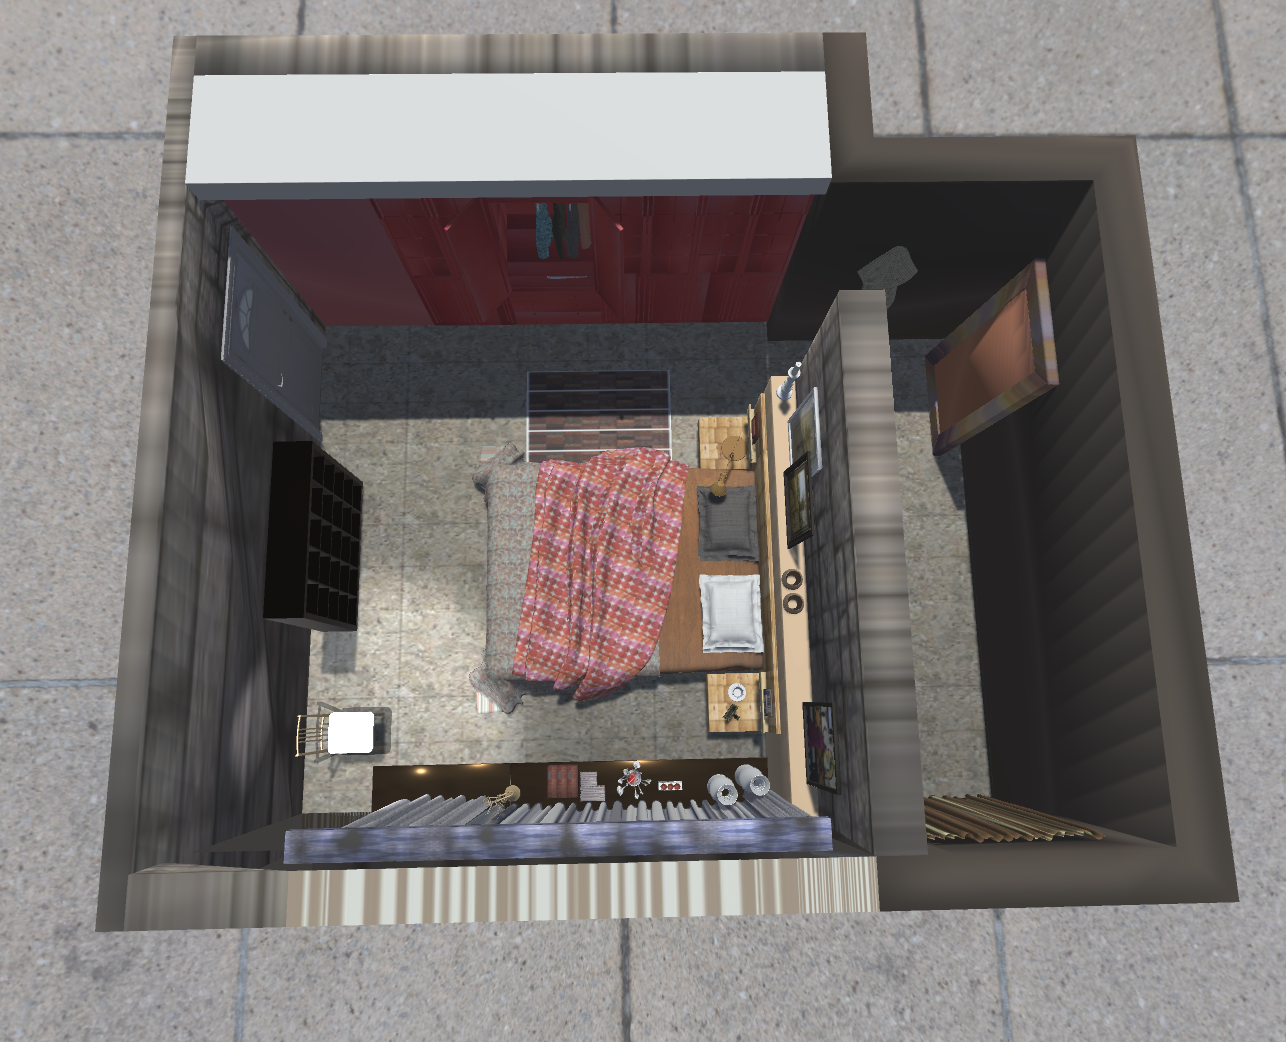
\includegraphics[width=.35\textwidth, height = .35\textwidth]{/Users/apple/OVGU/Thesis/code/3dReconstruction/report/images/implementation/scenenet_scenes/scene_bedroom}}\quad
    \subfloat[][]{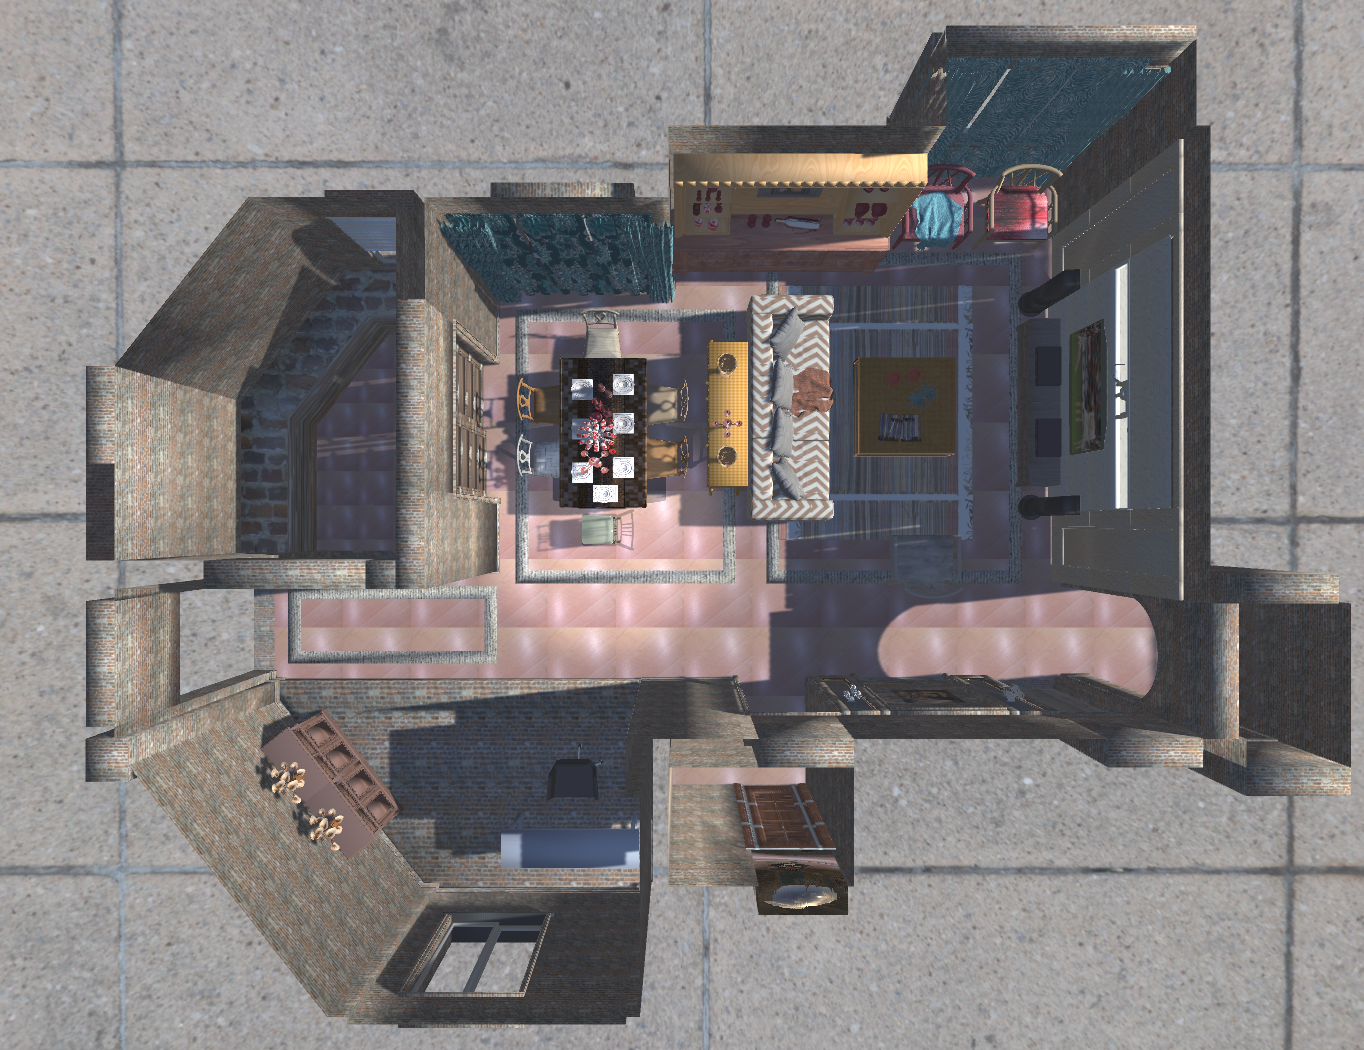
\includegraphics[width=.35\textwidth, height = .35\textwidth]{/Users/apple/OVGU/Thesis/code/3dReconstruction/report/images/implementation/scenenet_scenes/scene_livingroom}}\\
    \subfloat[][]{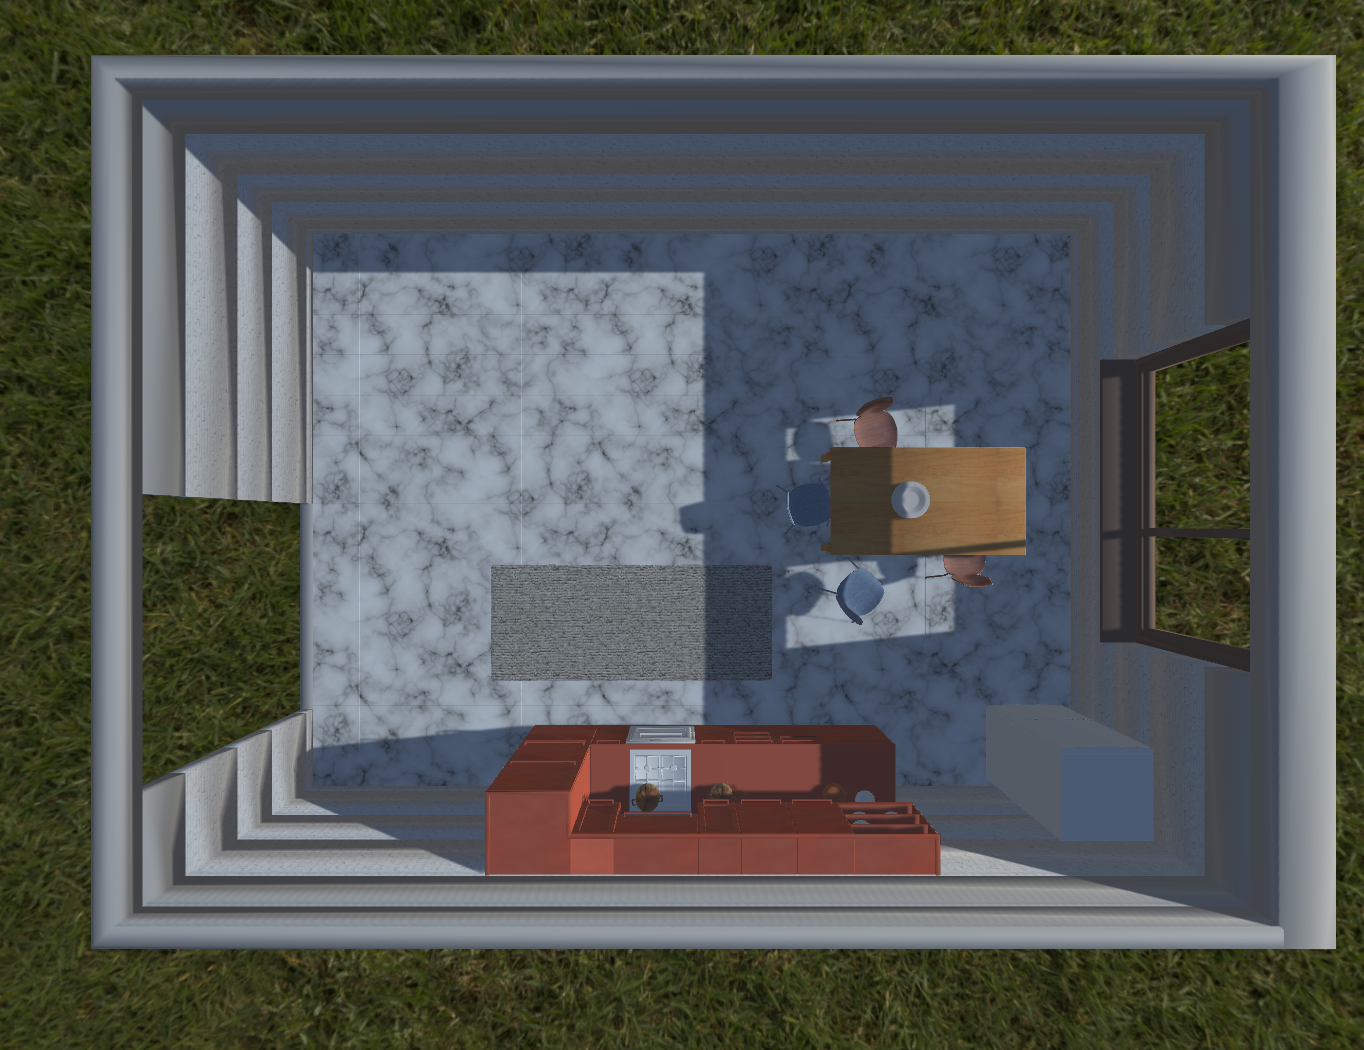
\includegraphics[width=.35\textwidth, height = .35\textwidth]{/Users/apple/OVGU/Thesis/code/3dReconstruction/report/images/implementation/scenenet_scenes/scene_kitchen}}\quad
    \subfloat[][]{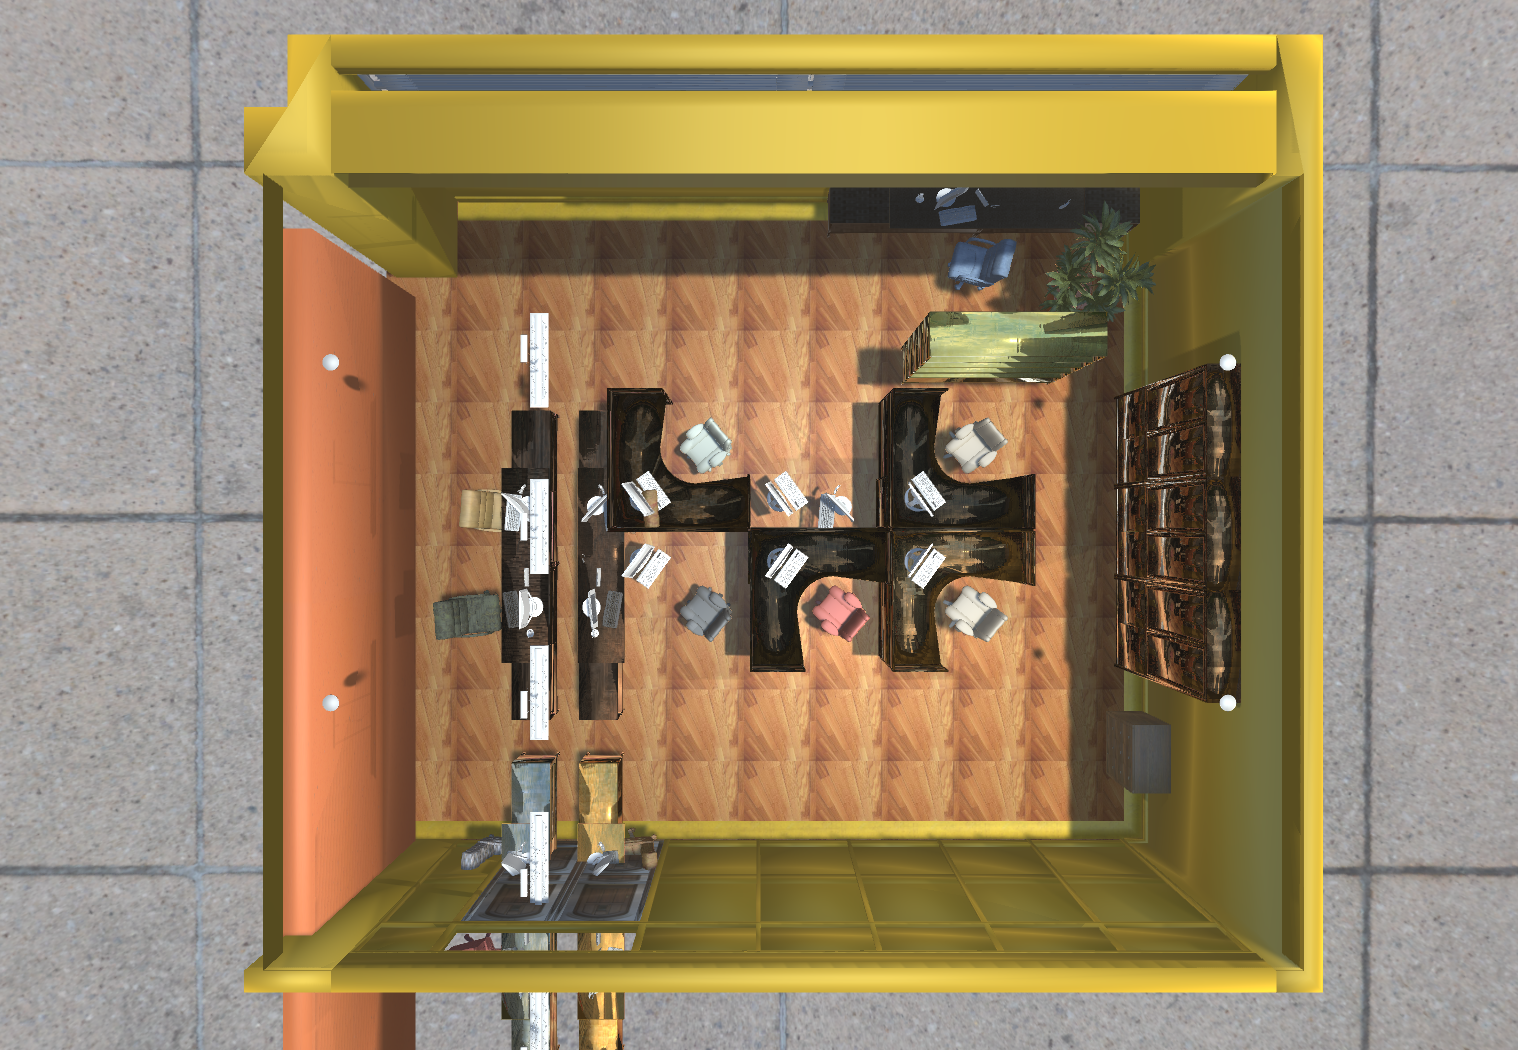
\includegraphics[width=.35\textwidth, height = .35\textwidth]{/Users/apple/OVGU/Thesis/code/3dReconstruction/report/images/implementation/scenenet_scenes/scene_office}}
    \caption[Top View for SceneNet Layouts]{The top view of sample scene layouts from SceneNet. Types: (a)Bedroom, (b)LivingRoom, (c)Kitchen and (d)Office.}
    \label{fig:Scene Types}
\end{figure}

\subsection{Randomized Texture}\label{subsec:randomised-texture}

SceneNet~\cite{McCormac2017} also provide textures for different categories in the scene.
We further increase the texture database by adding more textures from ambientCG.com, which provides free licenses.
A total of 982 texture images with 58 regular object categories, some of which are just JPG or PNG images, while there are few textures from cgtextures\footnote{https://www.textures.com/} with more details like normals, displacement, and roughness.
This makes the textures more realistic.
The distribution of the top 40 texture categories used for randomization of scenes is as shown in \autoref{fig:Distribution of textures}, with categories of Pix3D
having a higher number of images.
Each scene is randomized for every snap taken of the target object.
Samples of texture randomization of background in the scene with the target object in focus are shown in \autoref{fig:Texture Randomisation}.

The textures need to be grouped together into a folder with category names.
Since this library is external to Unity, the users can add or remove textures according to their preferences.
Even new categories can be added by just creating a new folder.

\begin{figure}[!ht]
    \centering
    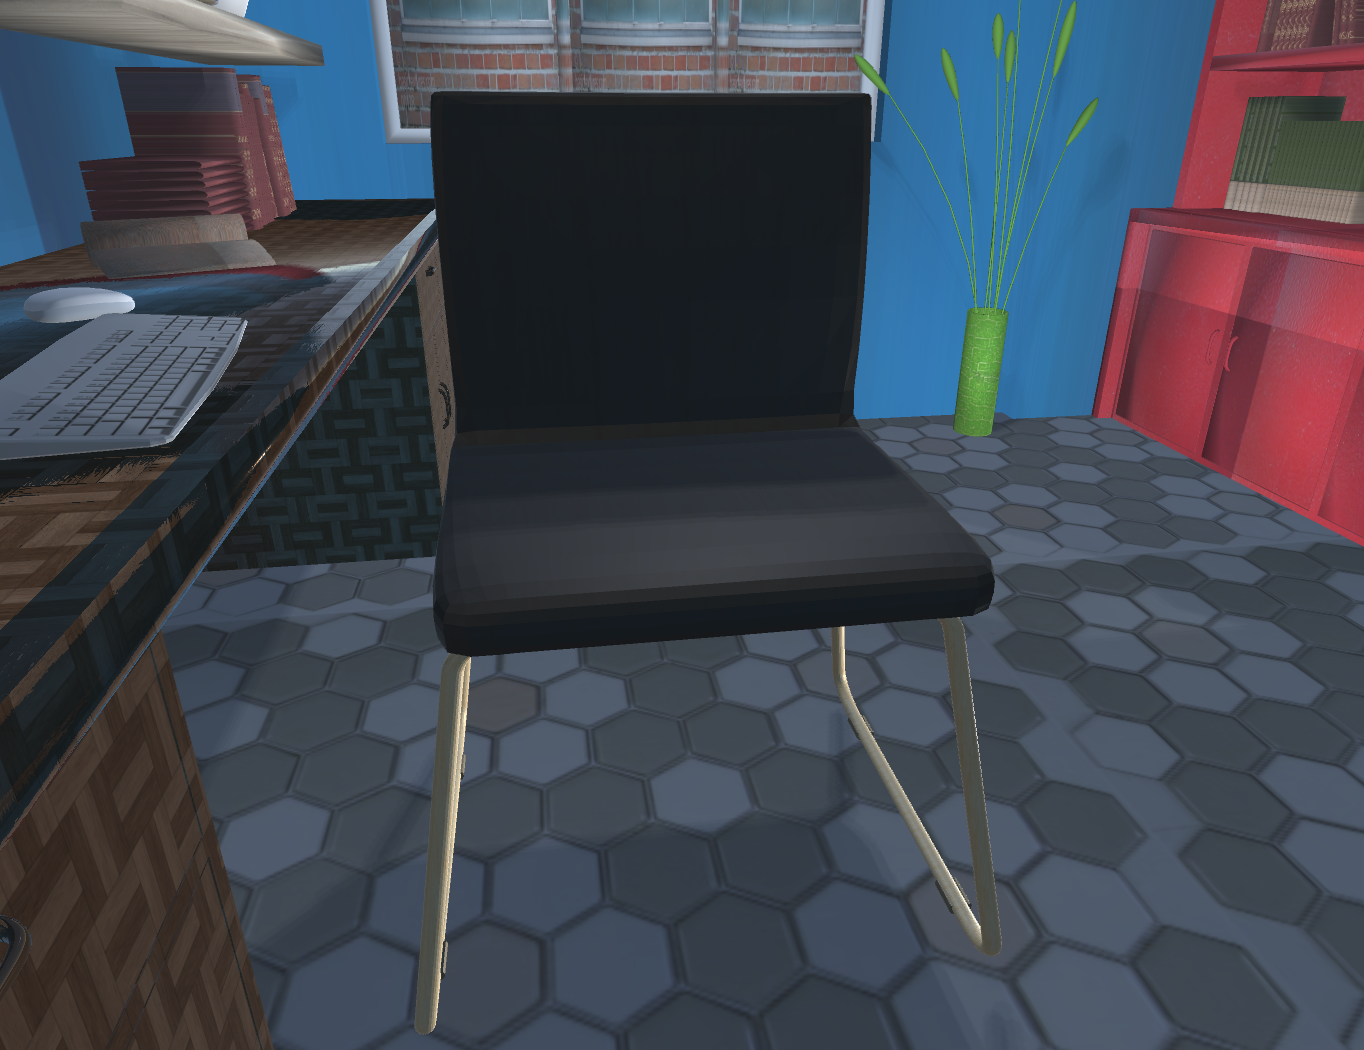
\includegraphics[width=.4\textwidth, height = .3\textwidth,valign=m]{/Users/apple/OVGU/Thesis/code/3dReconstruction/report/images/implementation/randomisation/background_texture1}
    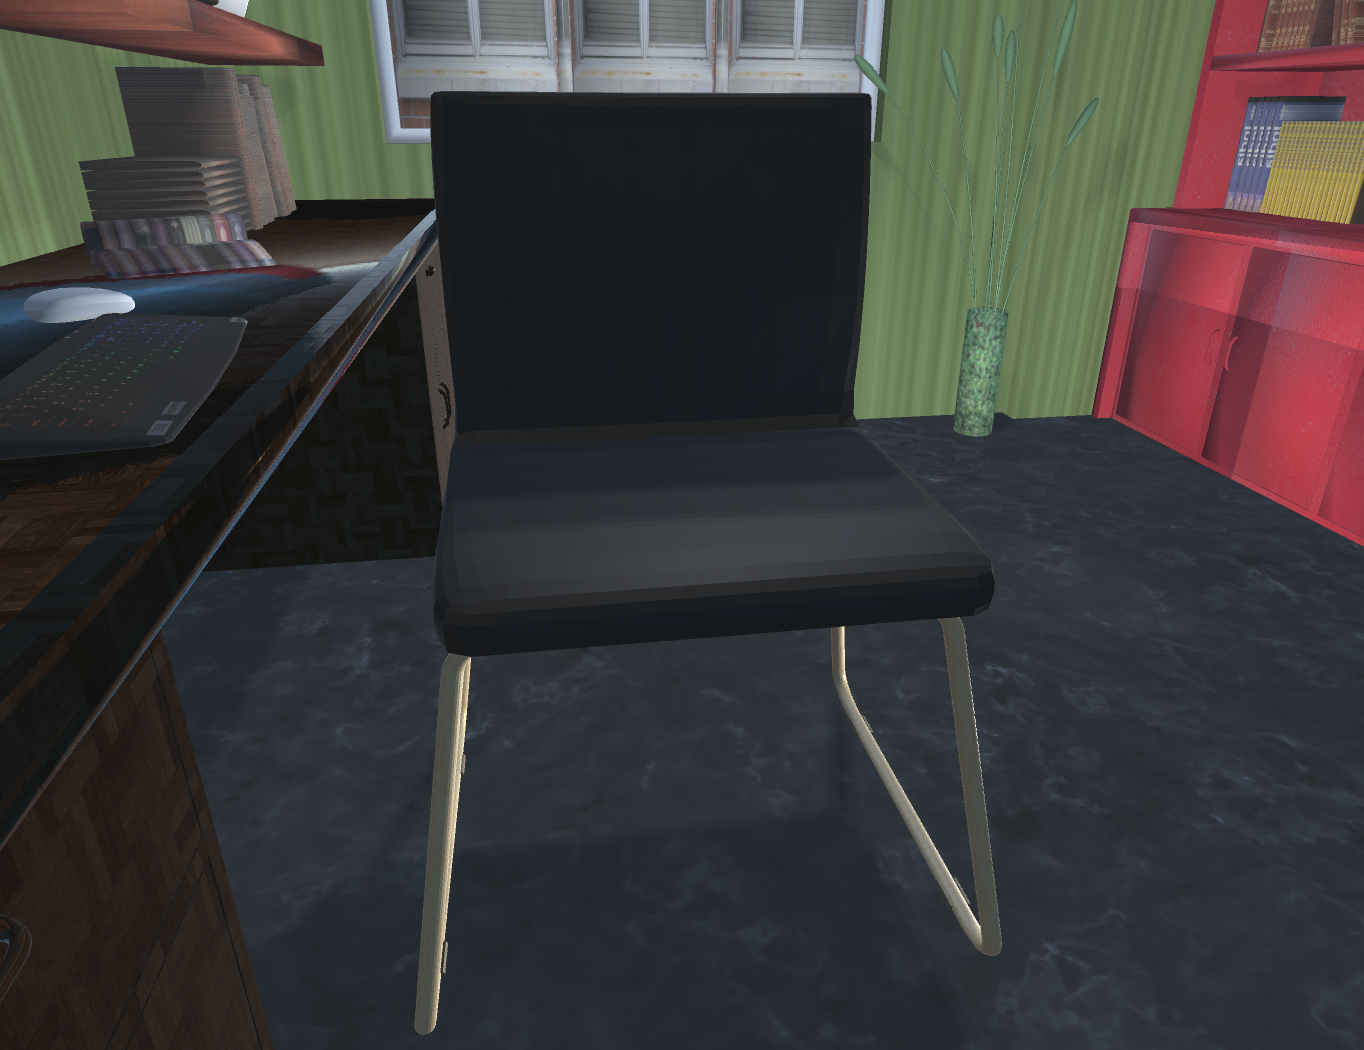
\includegraphics[width=.4\textwidth, height = .3\textwidth,valign=m]{/Users/apple/OVGU/Thesis/code/3dReconstruction/report/images/implementation/randomisation/background_texture2}\\
    \vspace{0.1cm}
    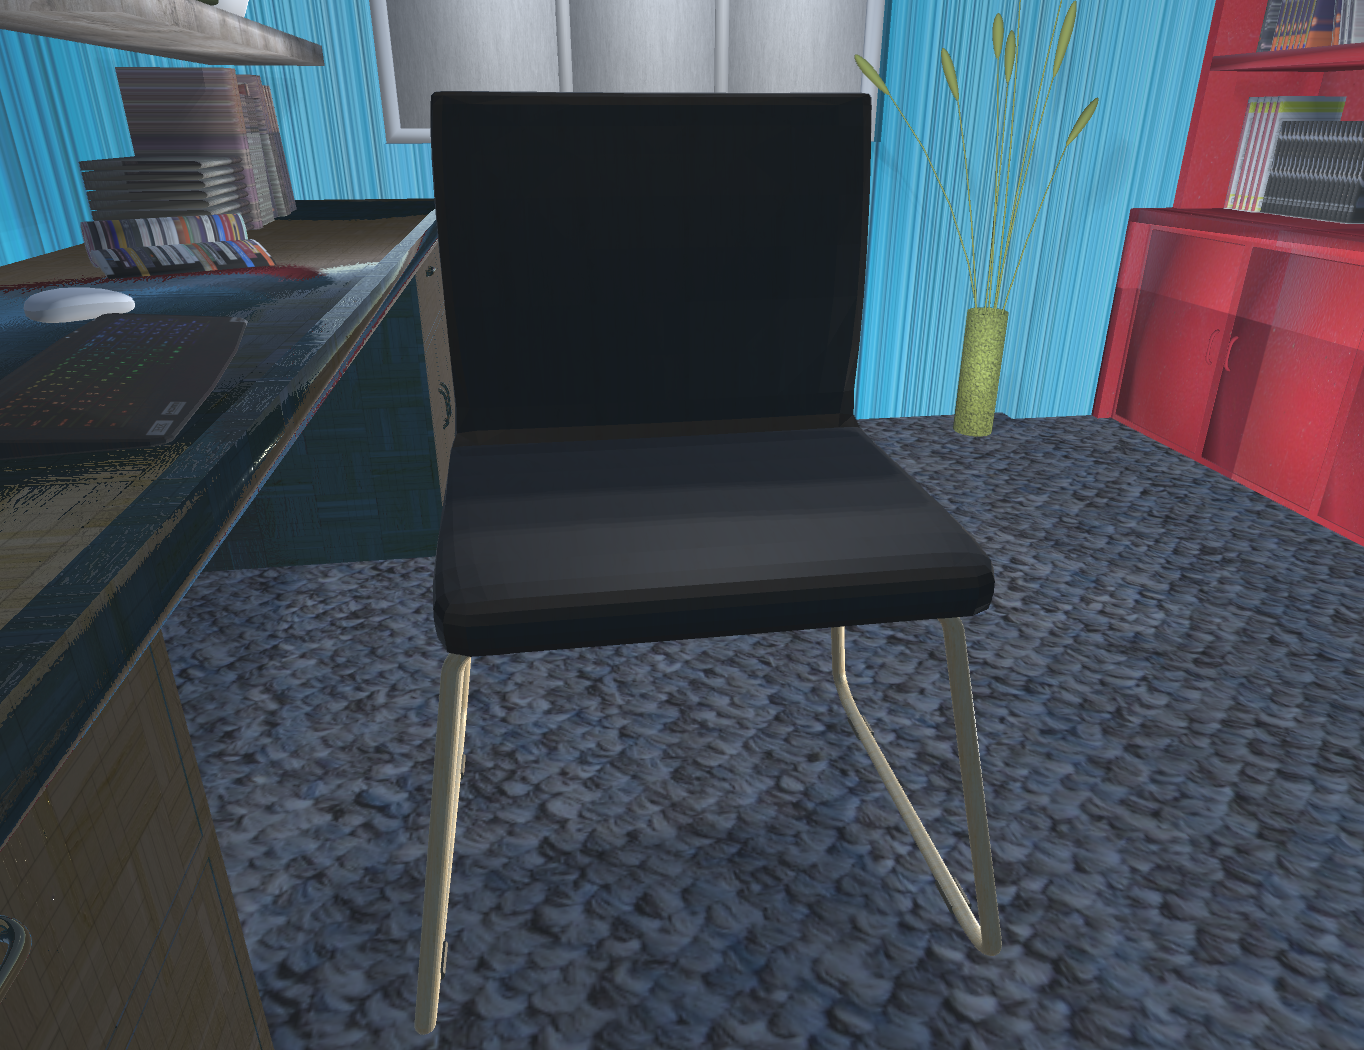
\includegraphics[width=.4\textwidth, height = .3\textwidth,valign=m]{/Users/apple/OVGU/Thesis/code/3dReconstruction/report/images/implementation/randomisation/background_texture3}
    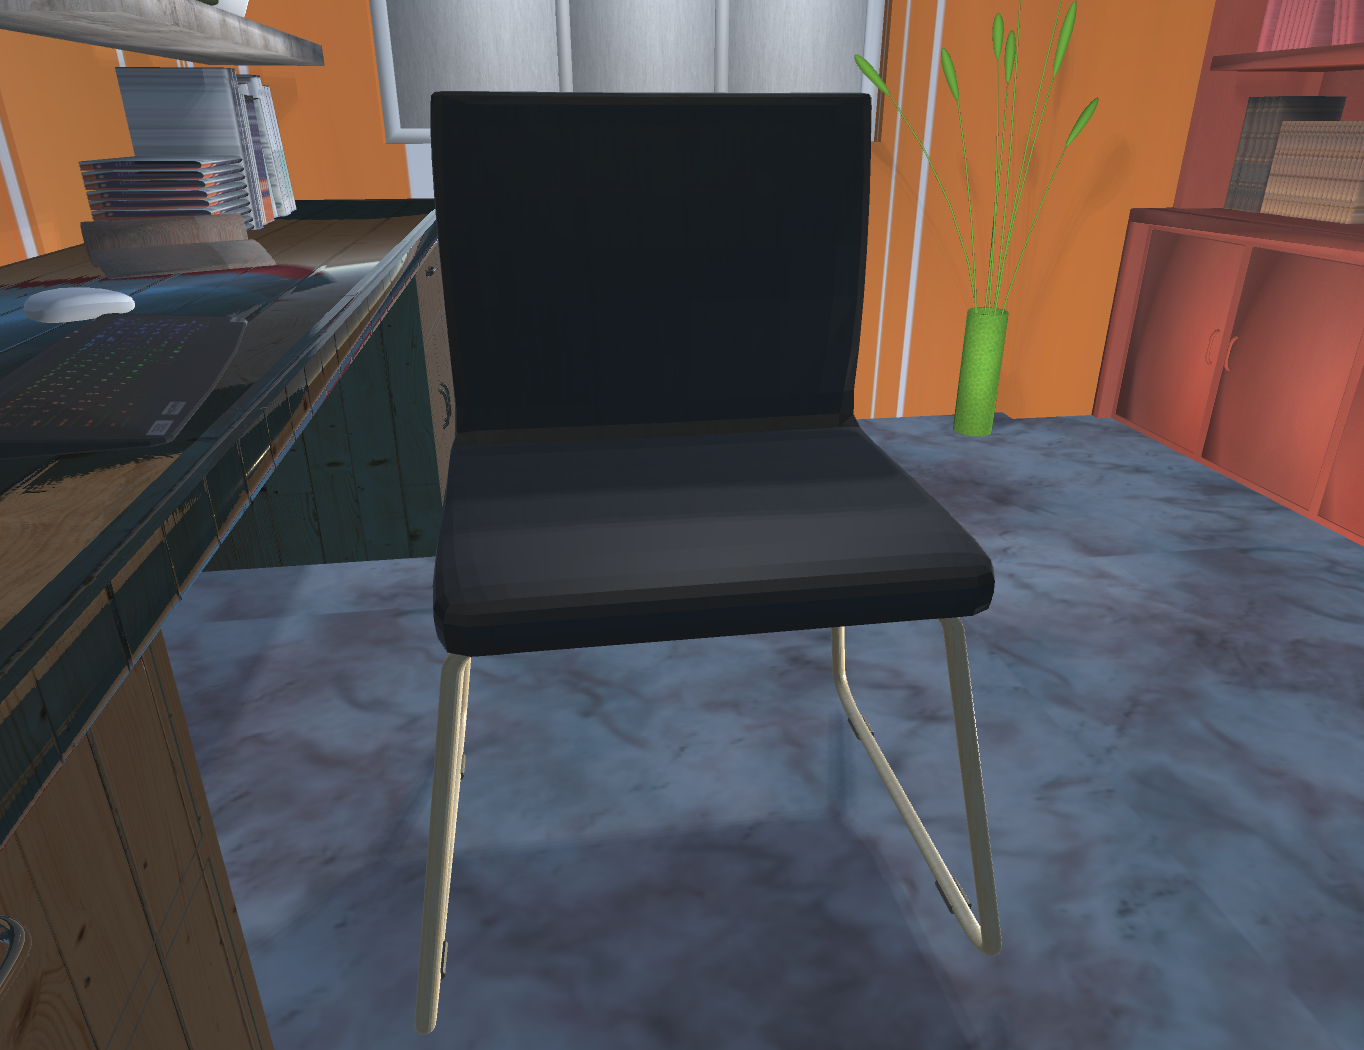
\includegraphics[width=.4\textwidth, height = .3\textwidth,valign=m]{/Users/apple/OVGU/Thesis/code/3dReconstruction/report/images/implementation/randomisation/background_texture4}\\
    \caption[Samples for Different Textures.]{Sample images with different textures for same scene.}
    \label{fig:Texture Randomisation}
\end{figure}

\begin{figure}[!ht]
    \centering
    \resizebox{\textwidth}{11.5cm}{%% Creator: Matplotlib, PGF backend
%%
%% To include the figure in your LaTeX document, write
%%   \input{<filename>.pgf}
%%
%% Make sure the required packages are loaded in your preamble
%%   \usepackage{pgf}
%%
%% Figures using additional raster images can only be included by \input if
%% they are in the same directory as the main LaTeX file. For loading figures
%% from other directories you can use the `import` package
%%   \usepackage{import}
%%
%% and then include the figures with
%%   \import{<path to file>}{<filename>.pgf}
%%
%% Matplotlib used the following preamble
%%   \usepackage{fontspec}
%%   \setmainfont{DejaVuSerif.ttf}[Path=\detokenize{/Users/apple/opt/anaconda3/envs/kaolin/lib/python3.7/site-packages/matplotlib/mpl-data/fonts/ttf/}]
%%   \setsansfont{DejaVuSans.ttf}[Path=\detokenize{/Users/apple/opt/anaconda3/envs/kaolin/lib/python3.7/site-packages/matplotlib/mpl-data/fonts/ttf/}]
%%   \setmonofont{DejaVuSansMono.ttf}[Path=\detokenize{/Users/apple/opt/anaconda3/envs/kaolin/lib/python3.7/site-packages/matplotlib/mpl-data/fonts/ttf/}]
%%
\begingroup%
\makeatletter%
\begin{pgfpicture}%
\pgfpathrectangle{\pgfpointorigin}{\pgfqpoint{5.522318in}{4.872128in}}%
\pgfusepath{use as bounding box, clip}%
\begin{pgfscope}%
\pgfsetbuttcap%
\pgfsetmiterjoin%
\definecolor{currentfill}{rgb}{1.000000,1.000000,1.000000}%
\pgfsetfillcolor{currentfill}%
\pgfsetlinewidth{0.000000pt}%
\definecolor{currentstroke}{rgb}{1.000000,1.000000,1.000000}%
\pgfsetstrokecolor{currentstroke}%
\pgfsetdash{}{0pt}%
\pgfpathmoveto{\pgfqpoint{0.000000in}{0.000000in}}%
\pgfpathlineto{\pgfqpoint{5.522318in}{0.000000in}}%
\pgfpathlineto{\pgfqpoint{5.522318in}{4.872128in}}%
\pgfpathlineto{\pgfqpoint{0.000000in}{4.872128in}}%
\pgfpathclose%
\pgfusepath{fill}%
\end{pgfscope}%
\begin{pgfscope}%
\pgfsetbuttcap%
\pgfsetmiterjoin%
\definecolor{currentfill}{rgb}{1.000000,1.000000,1.000000}%
\pgfsetfillcolor{currentfill}%
\pgfsetlinewidth{0.000000pt}%
\definecolor{currentstroke}{rgb}{0.000000,0.000000,0.000000}%
\pgfsetstrokecolor{currentstroke}%
\pgfsetstrokeopacity{0.000000}%
\pgfsetdash{}{0pt}%
\pgfpathmoveto{\pgfqpoint{0.462318in}{0.866167in}}%
\pgfpathlineto{\pgfqpoint{5.422318in}{0.866167in}}%
\pgfpathlineto{\pgfqpoint{5.422318in}{4.562168in}}%
\pgfpathlineto{\pgfqpoint{0.462318in}{4.562168in}}%
\pgfpathclose%
\pgfusepath{fill}%
\end{pgfscope}%
\begin{pgfscope}%
\pgfpathrectangle{\pgfqpoint{0.462318in}{0.866167in}}{\pgfqpoint{4.960000in}{3.696000in}}%
\pgfusepath{clip}%
\pgfsetbuttcap%
\pgfsetmiterjoin%
\definecolor{currentfill}{rgb}{0.000000,0.000000,1.000000}%
\pgfsetfillcolor{currentfill}%
\pgfsetlinewidth{0.000000pt}%
\definecolor{currentstroke}{rgb}{0.000000,0.000000,0.000000}%
\pgfsetstrokecolor{currentstroke}%
\pgfsetstrokeopacity{0.000000}%
\pgfsetdash{}{0pt}%
\pgfpathmoveto{\pgfqpoint{0.687773in}{0.866167in}}%
\pgfpathlineto{\pgfqpoint{0.778408in}{0.866167in}}%
\pgfpathlineto{\pgfqpoint{0.778408in}{4.386167in}}%
\pgfpathlineto{\pgfqpoint{0.687773in}{4.386167in}}%
\pgfpathclose%
\pgfusepath{fill}%
\end{pgfscope}%
\begin{pgfscope}%
\pgfpathrectangle{\pgfqpoint{0.462318in}{0.866167in}}{\pgfqpoint{4.960000in}{3.696000in}}%
\pgfusepath{clip}%
\pgfsetbuttcap%
\pgfsetmiterjoin%
\definecolor{currentfill}{rgb}{0.000000,0.000000,1.000000}%
\pgfsetfillcolor{currentfill}%
\pgfsetlinewidth{0.000000pt}%
\definecolor{currentstroke}{rgb}{0.000000,0.000000,0.000000}%
\pgfsetstrokecolor{currentstroke}%
\pgfsetstrokeopacity{0.000000}%
\pgfsetdash{}{0pt}%
\pgfpathmoveto{\pgfqpoint{0.801066in}{0.866167in}}%
\pgfpathlineto{\pgfqpoint{0.891701in}{0.866167in}}%
\pgfpathlineto{\pgfqpoint{0.891701in}{4.023281in}}%
\pgfpathlineto{\pgfqpoint{0.801066in}{4.023281in}}%
\pgfpathclose%
\pgfusepath{fill}%
\end{pgfscope}%
\begin{pgfscope}%
\pgfpathrectangle{\pgfqpoint{0.462318in}{0.866167in}}{\pgfqpoint{4.960000in}{3.696000in}}%
\pgfusepath{clip}%
\pgfsetbuttcap%
\pgfsetmiterjoin%
\definecolor{currentfill}{rgb}{0.000000,0.000000,1.000000}%
\pgfsetfillcolor{currentfill}%
\pgfsetlinewidth{0.000000pt}%
\definecolor{currentstroke}{rgb}{0.000000,0.000000,0.000000}%
\pgfsetstrokecolor{currentstroke}%
\pgfsetstrokeopacity{0.000000}%
\pgfsetdash{}{0pt}%
\pgfpathmoveto{\pgfqpoint{0.914360in}{0.866167in}}%
\pgfpathlineto{\pgfqpoint{1.004995in}{0.866167in}}%
\pgfpathlineto{\pgfqpoint{1.004995in}{2.825755in}}%
\pgfpathlineto{\pgfqpoint{0.914360in}{2.825755in}}%
\pgfpathclose%
\pgfusepath{fill}%
\end{pgfscope}%
\begin{pgfscope}%
\pgfpathrectangle{\pgfqpoint{0.462318in}{0.866167in}}{\pgfqpoint{4.960000in}{3.696000in}}%
\pgfusepath{clip}%
\pgfsetbuttcap%
\pgfsetmiterjoin%
\definecolor{currentfill}{rgb}{0.000000,0.000000,1.000000}%
\pgfsetfillcolor{currentfill}%
\pgfsetlinewidth{0.000000pt}%
\definecolor{currentstroke}{rgb}{0.000000,0.000000,0.000000}%
\pgfsetstrokecolor{currentstroke}%
\pgfsetstrokeopacity{0.000000}%
\pgfsetdash{}{0pt}%
\pgfpathmoveto{\pgfqpoint{1.027654in}{0.866167in}}%
\pgfpathlineto{\pgfqpoint{1.118289in}{0.866167in}}%
\pgfpathlineto{\pgfqpoint{1.118289in}{2.716889in}}%
\pgfpathlineto{\pgfqpoint{1.027654in}{2.716889in}}%
\pgfpathclose%
\pgfusepath{fill}%
\end{pgfscope}%
\begin{pgfscope}%
\pgfpathrectangle{\pgfqpoint{0.462318in}{0.866167in}}{\pgfqpoint{4.960000in}{3.696000in}}%
\pgfusepath{clip}%
\pgfsetbuttcap%
\pgfsetmiterjoin%
\definecolor{currentfill}{rgb}{0.000000,0.000000,1.000000}%
\pgfsetfillcolor{currentfill}%
\pgfsetlinewidth{0.000000pt}%
\definecolor{currentstroke}{rgb}{0.000000,0.000000,0.000000}%
\pgfsetstrokecolor{currentstroke}%
\pgfsetstrokeopacity{0.000000}%
\pgfsetdash{}{0pt}%
\pgfpathmoveto{\pgfqpoint{1.140948in}{0.866167in}}%
\pgfpathlineto{\pgfqpoint{1.231583in}{0.866167in}}%
\pgfpathlineto{\pgfqpoint{1.231583in}{2.716889in}}%
\pgfpathlineto{\pgfqpoint{1.140948in}{2.716889in}}%
\pgfpathclose%
\pgfusepath{fill}%
\end{pgfscope}%
\begin{pgfscope}%
\pgfpathrectangle{\pgfqpoint{0.462318in}{0.866167in}}{\pgfqpoint{4.960000in}{3.696000in}}%
\pgfusepath{clip}%
\pgfsetbuttcap%
\pgfsetmiterjoin%
\definecolor{currentfill}{rgb}{0.000000,0.000000,1.000000}%
\pgfsetfillcolor{currentfill}%
\pgfsetlinewidth{0.000000pt}%
\definecolor{currentstroke}{rgb}{0.000000,0.000000,0.000000}%
\pgfsetstrokecolor{currentstroke}%
\pgfsetstrokeopacity{0.000000}%
\pgfsetdash{}{0pt}%
\pgfpathmoveto{\pgfqpoint{1.254241in}{0.866167in}}%
\pgfpathlineto{\pgfqpoint{1.344876in}{0.866167in}}%
\pgfpathlineto{\pgfqpoint{1.344876in}{2.716889in}}%
\pgfpathlineto{\pgfqpoint{1.254241in}{2.716889in}}%
\pgfpathclose%
\pgfusepath{fill}%
\end{pgfscope}%
\begin{pgfscope}%
\pgfpathrectangle{\pgfqpoint{0.462318in}{0.866167in}}{\pgfqpoint{4.960000in}{3.696000in}}%
\pgfusepath{clip}%
\pgfsetbuttcap%
\pgfsetmiterjoin%
\definecolor{currentfill}{rgb}{0.000000,0.000000,1.000000}%
\pgfsetfillcolor{currentfill}%
\pgfsetlinewidth{0.000000pt}%
\definecolor{currentstroke}{rgb}{0.000000,0.000000,0.000000}%
\pgfsetstrokecolor{currentstroke}%
\pgfsetstrokeopacity{0.000000}%
\pgfsetdash{}{0pt}%
\pgfpathmoveto{\pgfqpoint{1.367535in}{0.866167in}}%
\pgfpathlineto{\pgfqpoint{1.458170in}{0.866167in}}%
\pgfpathlineto{\pgfqpoint{1.458170in}{2.571735in}}%
\pgfpathlineto{\pgfqpoint{1.367535in}{2.571735in}}%
\pgfpathclose%
\pgfusepath{fill}%
\end{pgfscope}%
\begin{pgfscope}%
\pgfpathrectangle{\pgfqpoint{0.462318in}{0.866167in}}{\pgfqpoint{4.960000in}{3.696000in}}%
\pgfusepath{clip}%
\pgfsetbuttcap%
\pgfsetmiterjoin%
\definecolor{currentfill}{rgb}{0.000000,0.000000,1.000000}%
\pgfsetfillcolor{currentfill}%
\pgfsetlinewidth{0.000000pt}%
\definecolor{currentstroke}{rgb}{0.000000,0.000000,0.000000}%
\pgfsetstrokecolor{currentstroke}%
\pgfsetstrokeopacity{0.000000}%
\pgfsetdash{}{0pt}%
\pgfpathmoveto{\pgfqpoint{1.480829in}{0.866167in}}%
\pgfpathlineto{\pgfqpoint{1.571464in}{0.866167in}}%
\pgfpathlineto{\pgfqpoint{1.571464in}{2.354003in}}%
\pgfpathlineto{\pgfqpoint{1.480829in}{2.354003in}}%
\pgfpathclose%
\pgfusepath{fill}%
\end{pgfscope}%
\begin{pgfscope}%
\pgfpathrectangle{\pgfqpoint{0.462318in}{0.866167in}}{\pgfqpoint{4.960000in}{3.696000in}}%
\pgfusepath{clip}%
\pgfsetbuttcap%
\pgfsetmiterjoin%
\definecolor{currentfill}{rgb}{0.000000,0.000000,1.000000}%
\pgfsetfillcolor{currentfill}%
\pgfsetlinewidth{0.000000pt}%
\definecolor{currentstroke}{rgb}{0.000000,0.000000,0.000000}%
\pgfsetstrokecolor{currentstroke}%
\pgfsetstrokeopacity{0.000000}%
\pgfsetdash{}{0pt}%
\pgfpathmoveto{\pgfqpoint{1.594123in}{0.866167in}}%
\pgfpathlineto{\pgfqpoint{1.684758in}{0.866167in}}%
\pgfpathlineto{\pgfqpoint{1.684758in}{2.208848in}}%
\pgfpathlineto{\pgfqpoint{1.594123in}{2.208848in}}%
\pgfpathclose%
\pgfusepath{fill}%
\end{pgfscope}%
\begin{pgfscope}%
\pgfpathrectangle{\pgfqpoint{0.462318in}{0.866167in}}{\pgfqpoint{4.960000in}{3.696000in}}%
\pgfusepath{clip}%
\pgfsetbuttcap%
\pgfsetmiterjoin%
\definecolor{currentfill}{rgb}{0.000000,0.000000,1.000000}%
\pgfsetfillcolor{currentfill}%
\pgfsetlinewidth{0.000000pt}%
\definecolor{currentstroke}{rgb}{0.000000,0.000000,0.000000}%
\pgfsetstrokecolor{currentstroke}%
\pgfsetstrokeopacity{0.000000}%
\pgfsetdash{}{0pt}%
\pgfpathmoveto{\pgfqpoint{1.707416in}{0.866167in}}%
\pgfpathlineto{\pgfqpoint{1.798051in}{0.866167in}}%
\pgfpathlineto{\pgfqpoint{1.798051in}{1.918539in}}%
\pgfpathlineto{\pgfqpoint{1.707416in}{1.918539in}}%
\pgfpathclose%
\pgfusepath{fill}%
\end{pgfscope}%
\begin{pgfscope}%
\pgfpathrectangle{\pgfqpoint{0.462318in}{0.866167in}}{\pgfqpoint{4.960000in}{3.696000in}}%
\pgfusepath{clip}%
\pgfsetbuttcap%
\pgfsetmiterjoin%
\definecolor{currentfill}{rgb}{0.000000,0.000000,1.000000}%
\pgfsetfillcolor{currentfill}%
\pgfsetlinewidth{0.000000pt}%
\definecolor{currentstroke}{rgb}{0.000000,0.000000,0.000000}%
\pgfsetstrokecolor{currentstroke}%
\pgfsetstrokeopacity{0.000000}%
\pgfsetdash{}{0pt}%
\pgfpathmoveto{\pgfqpoint{1.820710in}{0.866167in}}%
\pgfpathlineto{\pgfqpoint{1.911345in}{0.866167in}}%
\pgfpathlineto{\pgfqpoint{1.911345in}{1.882250in}}%
\pgfpathlineto{\pgfqpoint{1.820710in}{1.882250in}}%
\pgfpathclose%
\pgfusepath{fill}%
\end{pgfscope}%
\begin{pgfscope}%
\pgfpathrectangle{\pgfqpoint{0.462318in}{0.866167in}}{\pgfqpoint{4.960000in}{3.696000in}}%
\pgfusepath{clip}%
\pgfsetbuttcap%
\pgfsetmiterjoin%
\definecolor{currentfill}{rgb}{0.000000,0.000000,1.000000}%
\pgfsetfillcolor{currentfill}%
\pgfsetlinewidth{0.000000pt}%
\definecolor{currentstroke}{rgb}{0.000000,0.000000,0.000000}%
\pgfsetstrokecolor{currentstroke}%
\pgfsetstrokeopacity{0.000000}%
\pgfsetdash{}{0pt}%
\pgfpathmoveto{\pgfqpoint{1.934004in}{0.866167in}}%
\pgfpathlineto{\pgfqpoint{2.024639in}{0.866167in}}%
\pgfpathlineto{\pgfqpoint{2.024639in}{1.882250in}}%
\pgfpathlineto{\pgfqpoint{1.934004in}{1.882250in}}%
\pgfpathclose%
\pgfusepath{fill}%
\end{pgfscope}%
\begin{pgfscope}%
\pgfpathrectangle{\pgfqpoint{0.462318in}{0.866167in}}{\pgfqpoint{4.960000in}{3.696000in}}%
\pgfusepath{clip}%
\pgfsetbuttcap%
\pgfsetmiterjoin%
\definecolor{currentfill}{rgb}{0.000000,0.000000,1.000000}%
\pgfsetfillcolor{currentfill}%
\pgfsetlinewidth{0.000000pt}%
\definecolor{currentstroke}{rgb}{0.000000,0.000000,0.000000}%
\pgfsetstrokecolor{currentstroke}%
\pgfsetstrokeopacity{0.000000}%
\pgfsetdash{}{0pt}%
\pgfpathmoveto{\pgfqpoint{2.047298in}{0.866167in}}%
\pgfpathlineto{\pgfqpoint{2.137933in}{0.866167in}}%
\pgfpathlineto{\pgfqpoint{2.137933in}{1.845961in}}%
\pgfpathlineto{\pgfqpoint{2.047298in}{1.845961in}}%
\pgfpathclose%
\pgfusepath{fill}%
\end{pgfscope}%
\begin{pgfscope}%
\pgfpathrectangle{\pgfqpoint{0.462318in}{0.866167in}}{\pgfqpoint{4.960000in}{3.696000in}}%
\pgfusepath{clip}%
\pgfsetbuttcap%
\pgfsetmiterjoin%
\definecolor{currentfill}{rgb}{0.000000,0.000000,1.000000}%
\pgfsetfillcolor{currentfill}%
\pgfsetlinewidth{0.000000pt}%
\definecolor{currentstroke}{rgb}{0.000000,0.000000,0.000000}%
\pgfsetstrokecolor{currentstroke}%
\pgfsetstrokeopacity{0.000000}%
\pgfsetdash{}{0pt}%
\pgfpathmoveto{\pgfqpoint{2.160591in}{0.866167in}}%
\pgfpathlineto{\pgfqpoint{2.251226in}{0.866167in}}%
\pgfpathlineto{\pgfqpoint{2.251226in}{1.664518in}}%
\pgfpathlineto{\pgfqpoint{2.160591in}{1.664518in}}%
\pgfpathclose%
\pgfusepath{fill}%
\end{pgfscope}%
\begin{pgfscope}%
\pgfpathrectangle{\pgfqpoint{0.462318in}{0.866167in}}{\pgfqpoint{4.960000in}{3.696000in}}%
\pgfusepath{clip}%
\pgfsetbuttcap%
\pgfsetmiterjoin%
\definecolor{currentfill}{rgb}{0.000000,0.000000,1.000000}%
\pgfsetfillcolor{currentfill}%
\pgfsetlinewidth{0.000000pt}%
\definecolor{currentstroke}{rgb}{0.000000,0.000000,0.000000}%
\pgfsetstrokecolor{currentstroke}%
\pgfsetstrokeopacity{0.000000}%
\pgfsetdash{}{0pt}%
\pgfpathmoveto{\pgfqpoint{2.273885in}{0.866167in}}%
\pgfpathlineto{\pgfqpoint{2.364520in}{0.866167in}}%
\pgfpathlineto{\pgfqpoint{2.364520in}{1.664518in}}%
\pgfpathlineto{\pgfqpoint{2.273885in}{1.664518in}}%
\pgfpathclose%
\pgfusepath{fill}%
\end{pgfscope}%
\begin{pgfscope}%
\pgfpathrectangle{\pgfqpoint{0.462318in}{0.866167in}}{\pgfqpoint{4.960000in}{3.696000in}}%
\pgfusepath{clip}%
\pgfsetbuttcap%
\pgfsetmiterjoin%
\definecolor{currentfill}{rgb}{0.000000,0.000000,1.000000}%
\pgfsetfillcolor{currentfill}%
\pgfsetlinewidth{0.000000pt}%
\definecolor{currentstroke}{rgb}{0.000000,0.000000,0.000000}%
\pgfsetstrokecolor{currentstroke}%
\pgfsetstrokeopacity{0.000000}%
\pgfsetdash{}{0pt}%
\pgfpathmoveto{\pgfqpoint{2.387179in}{0.866167in}}%
\pgfpathlineto{\pgfqpoint{2.477814in}{0.866167in}}%
\pgfpathlineto{\pgfqpoint{2.477814in}{1.591941in}}%
\pgfpathlineto{\pgfqpoint{2.387179in}{1.591941in}}%
\pgfpathclose%
\pgfusepath{fill}%
\end{pgfscope}%
\begin{pgfscope}%
\pgfpathrectangle{\pgfqpoint{0.462318in}{0.866167in}}{\pgfqpoint{4.960000in}{3.696000in}}%
\pgfusepath{clip}%
\pgfsetbuttcap%
\pgfsetmiterjoin%
\definecolor{currentfill}{rgb}{0.000000,0.000000,1.000000}%
\pgfsetfillcolor{currentfill}%
\pgfsetlinewidth{0.000000pt}%
\definecolor{currentstroke}{rgb}{0.000000,0.000000,0.000000}%
\pgfsetstrokecolor{currentstroke}%
\pgfsetstrokeopacity{0.000000}%
\pgfsetdash{}{0pt}%
\pgfpathmoveto{\pgfqpoint{2.500473in}{0.866167in}}%
\pgfpathlineto{\pgfqpoint{2.591108in}{0.866167in}}%
\pgfpathlineto{\pgfqpoint{2.591108in}{1.446786in}}%
\pgfpathlineto{\pgfqpoint{2.500473in}{1.446786in}}%
\pgfpathclose%
\pgfusepath{fill}%
\end{pgfscope}%
\begin{pgfscope}%
\pgfpathrectangle{\pgfqpoint{0.462318in}{0.866167in}}{\pgfqpoint{4.960000in}{3.696000in}}%
\pgfusepath{clip}%
\pgfsetbuttcap%
\pgfsetmiterjoin%
\definecolor{currentfill}{rgb}{0.000000,0.000000,1.000000}%
\pgfsetfillcolor{currentfill}%
\pgfsetlinewidth{0.000000pt}%
\definecolor{currentstroke}{rgb}{0.000000,0.000000,0.000000}%
\pgfsetstrokecolor{currentstroke}%
\pgfsetstrokeopacity{0.000000}%
\pgfsetdash{}{0pt}%
\pgfpathmoveto{\pgfqpoint{2.613766in}{0.866167in}}%
\pgfpathlineto{\pgfqpoint{2.704401in}{0.866167in}}%
\pgfpathlineto{\pgfqpoint{2.704401in}{1.446786in}}%
\pgfpathlineto{\pgfqpoint{2.613766in}{1.446786in}}%
\pgfpathclose%
\pgfusepath{fill}%
\end{pgfscope}%
\begin{pgfscope}%
\pgfpathrectangle{\pgfqpoint{0.462318in}{0.866167in}}{\pgfqpoint{4.960000in}{3.696000in}}%
\pgfusepath{clip}%
\pgfsetbuttcap%
\pgfsetmiterjoin%
\definecolor{currentfill}{rgb}{0.000000,0.000000,1.000000}%
\pgfsetfillcolor{currentfill}%
\pgfsetlinewidth{0.000000pt}%
\definecolor{currentstroke}{rgb}{0.000000,0.000000,0.000000}%
\pgfsetstrokecolor{currentstroke}%
\pgfsetstrokeopacity{0.000000}%
\pgfsetdash{}{0pt}%
\pgfpathmoveto{\pgfqpoint{2.727060in}{0.866167in}}%
\pgfpathlineto{\pgfqpoint{2.817695in}{0.866167in}}%
\pgfpathlineto{\pgfqpoint{2.817695in}{1.446786in}}%
\pgfpathlineto{\pgfqpoint{2.727060in}{1.446786in}}%
\pgfpathclose%
\pgfusepath{fill}%
\end{pgfscope}%
\begin{pgfscope}%
\pgfpathrectangle{\pgfqpoint{0.462318in}{0.866167in}}{\pgfqpoint{4.960000in}{3.696000in}}%
\pgfusepath{clip}%
\pgfsetbuttcap%
\pgfsetmiterjoin%
\definecolor{currentfill}{rgb}{0.000000,0.000000,1.000000}%
\pgfsetfillcolor{currentfill}%
\pgfsetlinewidth{0.000000pt}%
\definecolor{currentstroke}{rgb}{0.000000,0.000000,0.000000}%
\pgfsetstrokecolor{currentstroke}%
\pgfsetstrokeopacity{0.000000}%
\pgfsetdash{}{0pt}%
\pgfpathmoveto{\pgfqpoint{2.840354in}{0.866167in}}%
\pgfpathlineto{\pgfqpoint{2.930989in}{0.866167in}}%
\pgfpathlineto{\pgfqpoint{2.930989in}{1.410497in}}%
\pgfpathlineto{\pgfqpoint{2.840354in}{1.410497in}}%
\pgfpathclose%
\pgfusepath{fill}%
\end{pgfscope}%
\begin{pgfscope}%
\pgfpathrectangle{\pgfqpoint{0.462318in}{0.866167in}}{\pgfqpoint{4.960000in}{3.696000in}}%
\pgfusepath{clip}%
\pgfsetbuttcap%
\pgfsetmiterjoin%
\definecolor{currentfill}{rgb}{0.000000,0.000000,1.000000}%
\pgfsetfillcolor{currentfill}%
\pgfsetlinewidth{0.000000pt}%
\definecolor{currentstroke}{rgb}{0.000000,0.000000,0.000000}%
\pgfsetstrokecolor{currentstroke}%
\pgfsetstrokeopacity{0.000000}%
\pgfsetdash{}{0pt}%
\pgfpathmoveto{\pgfqpoint{2.953648in}{0.866167in}}%
\pgfpathlineto{\pgfqpoint{3.044283in}{0.866167in}}%
\pgfpathlineto{\pgfqpoint{3.044283in}{1.374209in}}%
\pgfpathlineto{\pgfqpoint{2.953648in}{1.374209in}}%
\pgfpathclose%
\pgfusepath{fill}%
\end{pgfscope}%
\begin{pgfscope}%
\pgfpathrectangle{\pgfqpoint{0.462318in}{0.866167in}}{\pgfqpoint{4.960000in}{3.696000in}}%
\pgfusepath{clip}%
\pgfsetbuttcap%
\pgfsetmiterjoin%
\definecolor{currentfill}{rgb}{0.000000,0.000000,1.000000}%
\pgfsetfillcolor{currentfill}%
\pgfsetlinewidth{0.000000pt}%
\definecolor{currentstroke}{rgb}{0.000000,0.000000,0.000000}%
\pgfsetstrokecolor{currentstroke}%
\pgfsetstrokeopacity{0.000000}%
\pgfsetdash{}{0pt}%
\pgfpathmoveto{\pgfqpoint{3.066941in}{0.866167in}}%
\pgfpathlineto{\pgfqpoint{3.157576in}{0.866167in}}%
\pgfpathlineto{\pgfqpoint{3.157576in}{1.374209in}}%
\pgfpathlineto{\pgfqpoint{3.066941in}{1.374209in}}%
\pgfpathclose%
\pgfusepath{fill}%
\end{pgfscope}%
\begin{pgfscope}%
\pgfpathrectangle{\pgfqpoint{0.462318in}{0.866167in}}{\pgfqpoint{4.960000in}{3.696000in}}%
\pgfusepath{clip}%
\pgfsetbuttcap%
\pgfsetmiterjoin%
\definecolor{currentfill}{rgb}{0.000000,0.000000,1.000000}%
\pgfsetfillcolor{currentfill}%
\pgfsetlinewidth{0.000000pt}%
\definecolor{currentstroke}{rgb}{0.000000,0.000000,0.000000}%
\pgfsetstrokecolor{currentstroke}%
\pgfsetstrokeopacity{0.000000}%
\pgfsetdash{}{0pt}%
\pgfpathmoveto{\pgfqpoint{3.180235in}{0.866167in}}%
\pgfpathlineto{\pgfqpoint{3.270870in}{0.866167in}}%
\pgfpathlineto{\pgfqpoint{3.270870in}{1.374209in}}%
\pgfpathlineto{\pgfqpoint{3.180235in}{1.374209in}}%
\pgfpathclose%
\pgfusepath{fill}%
\end{pgfscope}%
\begin{pgfscope}%
\pgfpathrectangle{\pgfqpoint{0.462318in}{0.866167in}}{\pgfqpoint{4.960000in}{3.696000in}}%
\pgfusepath{clip}%
\pgfsetbuttcap%
\pgfsetmiterjoin%
\definecolor{currentfill}{rgb}{0.000000,0.000000,1.000000}%
\pgfsetfillcolor{currentfill}%
\pgfsetlinewidth{0.000000pt}%
\definecolor{currentstroke}{rgb}{0.000000,0.000000,0.000000}%
\pgfsetstrokecolor{currentstroke}%
\pgfsetstrokeopacity{0.000000}%
\pgfsetdash{}{0pt}%
\pgfpathmoveto{\pgfqpoint{3.293529in}{0.866167in}}%
\pgfpathlineto{\pgfqpoint{3.384164in}{0.866167in}}%
\pgfpathlineto{\pgfqpoint{3.384164in}{1.301631in}}%
\pgfpathlineto{\pgfqpoint{3.293529in}{1.301631in}}%
\pgfpathclose%
\pgfusepath{fill}%
\end{pgfscope}%
\begin{pgfscope}%
\pgfpathrectangle{\pgfqpoint{0.462318in}{0.866167in}}{\pgfqpoint{4.960000in}{3.696000in}}%
\pgfusepath{clip}%
\pgfsetbuttcap%
\pgfsetmiterjoin%
\definecolor{currentfill}{rgb}{0.000000,0.000000,1.000000}%
\pgfsetfillcolor{currentfill}%
\pgfsetlinewidth{0.000000pt}%
\definecolor{currentstroke}{rgb}{0.000000,0.000000,0.000000}%
\pgfsetstrokecolor{currentstroke}%
\pgfsetstrokeopacity{0.000000}%
\pgfsetdash{}{0pt}%
\pgfpathmoveto{\pgfqpoint{3.406823in}{0.866167in}}%
\pgfpathlineto{\pgfqpoint{3.497458in}{0.866167in}}%
\pgfpathlineto{\pgfqpoint{3.497458in}{1.301631in}}%
\pgfpathlineto{\pgfqpoint{3.406823in}{1.301631in}}%
\pgfpathclose%
\pgfusepath{fill}%
\end{pgfscope}%
\begin{pgfscope}%
\pgfpathrectangle{\pgfqpoint{0.462318in}{0.866167in}}{\pgfqpoint{4.960000in}{3.696000in}}%
\pgfusepath{clip}%
\pgfsetbuttcap%
\pgfsetmiterjoin%
\definecolor{currentfill}{rgb}{0.000000,0.000000,1.000000}%
\pgfsetfillcolor{currentfill}%
\pgfsetlinewidth{0.000000pt}%
\definecolor{currentstroke}{rgb}{0.000000,0.000000,0.000000}%
\pgfsetstrokecolor{currentstroke}%
\pgfsetstrokeopacity{0.000000}%
\pgfsetdash{}{0pt}%
\pgfpathmoveto{\pgfqpoint{3.520116in}{0.866167in}}%
\pgfpathlineto{\pgfqpoint{3.610751in}{0.866167in}}%
\pgfpathlineto{\pgfqpoint{3.610751in}{1.301631in}}%
\pgfpathlineto{\pgfqpoint{3.520116in}{1.301631in}}%
\pgfpathclose%
\pgfusepath{fill}%
\end{pgfscope}%
\begin{pgfscope}%
\pgfpathrectangle{\pgfqpoint{0.462318in}{0.866167in}}{\pgfqpoint{4.960000in}{3.696000in}}%
\pgfusepath{clip}%
\pgfsetbuttcap%
\pgfsetmiterjoin%
\definecolor{currentfill}{rgb}{0.000000,0.000000,1.000000}%
\pgfsetfillcolor{currentfill}%
\pgfsetlinewidth{0.000000pt}%
\definecolor{currentstroke}{rgb}{0.000000,0.000000,0.000000}%
\pgfsetstrokecolor{currentstroke}%
\pgfsetstrokeopacity{0.000000}%
\pgfsetdash{}{0pt}%
\pgfpathmoveto{\pgfqpoint{3.633410in}{0.866167in}}%
\pgfpathlineto{\pgfqpoint{3.724045in}{0.866167in}}%
\pgfpathlineto{\pgfqpoint{3.724045in}{1.156477in}}%
\pgfpathlineto{\pgfqpoint{3.633410in}{1.156477in}}%
\pgfpathclose%
\pgfusepath{fill}%
\end{pgfscope}%
\begin{pgfscope}%
\pgfpathrectangle{\pgfqpoint{0.462318in}{0.866167in}}{\pgfqpoint{4.960000in}{3.696000in}}%
\pgfusepath{clip}%
\pgfsetbuttcap%
\pgfsetmiterjoin%
\definecolor{currentfill}{rgb}{0.000000,0.000000,1.000000}%
\pgfsetfillcolor{currentfill}%
\pgfsetlinewidth{0.000000pt}%
\definecolor{currentstroke}{rgb}{0.000000,0.000000,0.000000}%
\pgfsetstrokecolor{currentstroke}%
\pgfsetstrokeopacity{0.000000}%
\pgfsetdash{}{0pt}%
\pgfpathmoveto{\pgfqpoint{3.746704in}{0.866167in}}%
\pgfpathlineto{\pgfqpoint{3.837339in}{0.866167in}}%
\pgfpathlineto{\pgfqpoint{3.837339in}{1.156477in}}%
\pgfpathlineto{\pgfqpoint{3.746704in}{1.156477in}}%
\pgfpathclose%
\pgfusepath{fill}%
\end{pgfscope}%
\begin{pgfscope}%
\pgfpathrectangle{\pgfqpoint{0.462318in}{0.866167in}}{\pgfqpoint{4.960000in}{3.696000in}}%
\pgfusepath{clip}%
\pgfsetbuttcap%
\pgfsetmiterjoin%
\definecolor{currentfill}{rgb}{0.000000,0.000000,1.000000}%
\pgfsetfillcolor{currentfill}%
\pgfsetlinewidth{0.000000pt}%
\definecolor{currentstroke}{rgb}{0.000000,0.000000,0.000000}%
\pgfsetstrokecolor{currentstroke}%
\pgfsetstrokeopacity{0.000000}%
\pgfsetdash{}{0pt}%
\pgfpathmoveto{\pgfqpoint{3.859998in}{0.866167in}}%
\pgfpathlineto{\pgfqpoint{3.950632in}{0.866167in}}%
\pgfpathlineto{\pgfqpoint{3.950632in}{1.120188in}}%
\pgfpathlineto{\pgfqpoint{3.859998in}{1.120188in}}%
\pgfpathclose%
\pgfusepath{fill}%
\end{pgfscope}%
\begin{pgfscope}%
\pgfpathrectangle{\pgfqpoint{0.462318in}{0.866167in}}{\pgfqpoint{4.960000in}{3.696000in}}%
\pgfusepath{clip}%
\pgfsetbuttcap%
\pgfsetmiterjoin%
\definecolor{currentfill}{rgb}{0.000000,0.000000,1.000000}%
\pgfsetfillcolor{currentfill}%
\pgfsetlinewidth{0.000000pt}%
\definecolor{currentstroke}{rgb}{0.000000,0.000000,0.000000}%
\pgfsetstrokecolor{currentstroke}%
\pgfsetstrokeopacity{0.000000}%
\pgfsetdash{}{0pt}%
\pgfpathmoveto{\pgfqpoint{3.973291in}{0.866167in}}%
\pgfpathlineto{\pgfqpoint{4.063926in}{0.866167in}}%
\pgfpathlineto{\pgfqpoint{4.063926in}{1.120188in}}%
\pgfpathlineto{\pgfqpoint{3.973291in}{1.120188in}}%
\pgfpathclose%
\pgfusepath{fill}%
\end{pgfscope}%
\begin{pgfscope}%
\pgfpathrectangle{\pgfqpoint{0.462318in}{0.866167in}}{\pgfqpoint{4.960000in}{3.696000in}}%
\pgfusepath{clip}%
\pgfsetbuttcap%
\pgfsetmiterjoin%
\definecolor{currentfill}{rgb}{0.000000,0.000000,1.000000}%
\pgfsetfillcolor{currentfill}%
\pgfsetlinewidth{0.000000pt}%
\definecolor{currentstroke}{rgb}{0.000000,0.000000,0.000000}%
\pgfsetstrokecolor{currentstroke}%
\pgfsetstrokeopacity{0.000000}%
\pgfsetdash{}{0pt}%
\pgfpathmoveto{\pgfqpoint{4.086585in}{0.866167in}}%
\pgfpathlineto{\pgfqpoint{4.177220in}{0.866167in}}%
\pgfpathlineto{\pgfqpoint{4.177220in}{1.120188in}}%
\pgfpathlineto{\pgfqpoint{4.086585in}{1.120188in}}%
\pgfpathclose%
\pgfusepath{fill}%
\end{pgfscope}%
\begin{pgfscope}%
\pgfpathrectangle{\pgfqpoint{0.462318in}{0.866167in}}{\pgfqpoint{4.960000in}{3.696000in}}%
\pgfusepath{clip}%
\pgfsetbuttcap%
\pgfsetmiterjoin%
\definecolor{currentfill}{rgb}{0.000000,0.000000,1.000000}%
\pgfsetfillcolor{currentfill}%
\pgfsetlinewidth{0.000000pt}%
\definecolor{currentstroke}{rgb}{0.000000,0.000000,0.000000}%
\pgfsetstrokecolor{currentstroke}%
\pgfsetstrokeopacity{0.000000}%
\pgfsetdash{}{0pt}%
\pgfpathmoveto{\pgfqpoint{4.199879in}{0.866167in}}%
\pgfpathlineto{\pgfqpoint{4.290514in}{0.866167in}}%
\pgfpathlineto{\pgfqpoint{4.290514in}{1.120188in}}%
\pgfpathlineto{\pgfqpoint{4.199879in}{1.120188in}}%
\pgfpathclose%
\pgfusepath{fill}%
\end{pgfscope}%
\begin{pgfscope}%
\pgfpathrectangle{\pgfqpoint{0.462318in}{0.866167in}}{\pgfqpoint{4.960000in}{3.696000in}}%
\pgfusepath{clip}%
\pgfsetbuttcap%
\pgfsetmiterjoin%
\definecolor{currentfill}{rgb}{0.000000,0.000000,1.000000}%
\pgfsetfillcolor{currentfill}%
\pgfsetlinewidth{0.000000pt}%
\definecolor{currentstroke}{rgb}{0.000000,0.000000,0.000000}%
\pgfsetstrokecolor{currentstroke}%
\pgfsetstrokeopacity{0.000000}%
\pgfsetdash{}{0pt}%
\pgfpathmoveto{\pgfqpoint{4.313172in}{0.866167in}}%
\pgfpathlineto{\pgfqpoint{4.403807in}{0.866167in}}%
\pgfpathlineto{\pgfqpoint{4.403807in}{1.083899in}}%
\pgfpathlineto{\pgfqpoint{4.313172in}{1.083899in}}%
\pgfpathclose%
\pgfusepath{fill}%
\end{pgfscope}%
\begin{pgfscope}%
\pgfpathrectangle{\pgfqpoint{0.462318in}{0.866167in}}{\pgfqpoint{4.960000in}{3.696000in}}%
\pgfusepath{clip}%
\pgfsetbuttcap%
\pgfsetmiterjoin%
\definecolor{currentfill}{rgb}{0.000000,0.000000,1.000000}%
\pgfsetfillcolor{currentfill}%
\pgfsetlinewidth{0.000000pt}%
\definecolor{currentstroke}{rgb}{0.000000,0.000000,0.000000}%
\pgfsetstrokecolor{currentstroke}%
\pgfsetstrokeopacity{0.000000}%
\pgfsetdash{}{0pt}%
\pgfpathmoveto{\pgfqpoint{4.426466in}{0.866167in}}%
\pgfpathlineto{\pgfqpoint{4.517101in}{0.866167in}}%
\pgfpathlineto{\pgfqpoint{4.517101in}{1.083899in}}%
\pgfpathlineto{\pgfqpoint{4.426466in}{1.083899in}}%
\pgfpathclose%
\pgfusepath{fill}%
\end{pgfscope}%
\begin{pgfscope}%
\pgfpathrectangle{\pgfqpoint{0.462318in}{0.866167in}}{\pgfqpoint{4.960000in}{3.696000in}}%
\pgfusepath{clip}%
\pgfsetbuttcap%
\pgfsetmiterjoin%
\definecolor{currentfill}{rgb}{0.000000,0.000000,1.000000}%
\pgfsetfillcolor{currentfill}%
\pgfsetlinewidth{0.000000pt}%
\definecolor{currentstroke}{rgb}{0.000000,0.000000,0.000000}%
\pgfsetstrokecolor{currentstroke}%
\pgfsetstrokeopacity{0.000000}%
\pgfsetdash{}{0pt}%
\pgfpathmoveto{\pgfqpoint{4.539760in}{0.866167in}}%
\pgfpathlineto{\pgfqpoint{4.630395in}{0.866167in}}%
\pgfpathlineto{\pgfqpoint{4.630395in}{1.083899in}}%
\pgfpathlineto{\pgfqpoint{4.539760in}{1.083899in}}%
\pgfpathclose%
\pgfusepath{fill}%
\end{pgfscope}%
\begin{pgfscope}%
\pgfpathrectangle{\pgfqpoint{0.462318in}{0.866167in}}{\pgfqpoint{4.960000in}{3.696000in}}%
\pgfusepath{clip}%
\pgfsetbuttcap%
\pgfsetmiterjoin%
\definecolor{currentfill}{rgb}{0.000000,0.000000,1.000000}%
\pgfsetfillcolor{currentfill}%
\pgfsetlinewidth{0.000000pt}%
\definecolor{currentstroke}{rgb}{0.000000,0.000000,0.000000}%
\pgfsetstrokecolor{currentstroke}%
\pgfsetstrokeopacity{0.000000}%
\pgfsetdash{}{0pt}%
\pgfpathmoveto{\pgfqpoint{4.653054in}{0.866167in}}%
\pgfpathlineto{\pgfqpoint{4.743689in}{0.866167in}}%
\pgfpathlineto{\pgfqpoint{4.743689in}{1.083899in}}%
\pgfpathlineto{\pgfqpoint{4.653054in}{1.083899in}}%
\pgfpathclose%
\pgfusepath{fill}%
\end{pgfscope}%
\begin{pgfscope}%
\pgfpathrectangle{\pgfqpoint{0.462318in}{0.866167in}}{\pgfqpoint{4.960000in}{3.696000in}}%
\pgfusepath{clip}%
\pgfsetbuttcap%
\pgfsetmiterjoin%
\definecolor{currentfill}{rgb}{0.000000,0.000000,1.000000}%
\pgfsetfillcolor{currentfill}%
\pgfsetlinewidth{0.000000pt}%
\definecolor{currentstroke}{rgb}{0.000000,0.000000,0.000000}%
\pgfsetstrokecolor{currentstroke}%
\pgfsetstrokeopacity{0.000000}%
\pgfsetdash{}{0pt}%
\pgfpathmoveto{\pgfqpoint{4.766347in}{0.866167in}}%
\pgfpathlineto{\pgfqpoint{4.856982in}{0.866167in}}%
\pgfpathlineto{\pgfqpoint{4.856982in}{1.083899in}}%
\pgfpathlineto{\pgfqpoint{4.766347in}{1.083899in}}%
\pgfpathclose%
\pgfusepath{fill}%
\end{pgfscope}%
\begin{pgfscope}%
\pgfpathrectangle{\pgfqpoint{0.462318in}{0.866167in}}{\pgfqpoint{4.960000in}{3.696000in}}%
\pgfusepath{clip}%
\pgfsetbuttcap%
\pgfsetmiterjoin%
\definecolor{currentfill}{rgb}{0.000000,0.000000,1.000000}%
\pgfsetfillcolor{currentfill}%
\pgfsetlinewidth{0.000000pt}%
\definecolor{currentstroke}{rgb}{0.000000,0.000000,0.000000}%
\pgfsetstrokecolor{currentstroke}%
\pgfsetstrokeopacity{0.000000}%
\pgfsetdash{}{0pt}%
\pgfpathmoveto{\pgfqpoint{4.879641in}{0.866167in}}%
\pgfpathlineto{\pgfqpoint{4.970276in}{0.866167in}}%
\pgfpathlineto{\pgfqpoint{4.970276in}{1.083899in}}%
\pgfpathlineto{\pgfqpoint{4.879641in}{1.083899in}}%
\pgfpathclose%
\pgfusepath{fill}%
\end{pgfscope}%
\begin{pgfscope}%
\pgfpathrectangle{\pgfqpoint{0.462318in}{0.866167in}}{\pgfqpoint{4.960000in}{3.696000in}}%
\pgfusepath{clip}%
\pgfsetbuttcap%
\pgfsetmiterjoin%
\definecolor{currentfill}{rgb}{0.000000,0.000000,1.000000}%
\pgfsetfillcolor{currentfill}%
\pgfsetlinewidth{0.000000pt}%
\definecolor{currentstroke}{rgb}{0.000000,0.000000,0.000000}%
\pgfsetstrokecolor{currentstroke}%
\pgfsetstrokeopacity{0.000000}%
\pgfsetdash{}{0pt}%
\pgfpathmoveto{\pgfqpoint{4.992935in}{0.866167in}}%
\pgfpathlineto{\pgfqpoint{5.083570in}{0.866167in}}%
\pgfpathlineto{\pgfqpoint{5.083570in}{1.083899in}}%
\pgfpathlineto{\pgfqpoint{4.992935in}{1.083899in}}%
\pgfpathclose%
\pgfusepath{fill}%
\end{pgfscope}%
\begin{pgfscope}%
\pgfpathrectangle{\pgfqpoint{0.462318in}{0.866167in}}{\pgfqpoint{4.960000in}{3.696000in}}%
\pgfusepath{clip}%
\pgfsetbuttcap%
\pgfsetmiterjoin%
\definecolor{currentfill}{rgb}{0.000000,0.000000,1.000000}%
\pgfsetfillcolor{currentfill}%
\pgfsetlinewidth{0.000000pt}%
\definecolor{currentstroke}{rgb}{0.000000,0.000000,0.000000}%
\pgfsetstrokecolor{currentstroke}%
\pgfsetstrokeopacity{0.000000}%
\pgfsetdash{}{0pt}%
\pgfpathmoveto{\pgfqpoint{5.106229in}{0.866167in}}%
\pgfpathlineto{\pgfqpoint{5.196864in}{0.866167in}}%
\pgfpathlineto{\pgfqpoint{5.196864in}{1.047611in}}%
\pgfpathlineto{\pgfqpoint{5.106229in}{1.047611in}}%
\pgfpathclose%
\pgfusepath{fill}%
\end{pgfscope}%
\begin{pgfscope}%
\pgfsetbuttcap%
\pgfsetroundjoin%
\definecolor{currentfill}{rgb}{0.000000,0.000000,0.000000}%
\pgfsetfillcolor{currentfill}%
\pgfsetlinewidth{0.803000pt}%
\definecolor{currentstroke}{rgb}{0.000000,0.000000,0.000000}%
\pgfsetstrokecolor{currentstroke}%
\pgfsetdash{}{0pt}%
\pgfsys@defobject{currentmarker}{\pgfqpoint{0.000000in}{-0.048611in}}{\pgfqpoint{0.000000in}{0.000000in}}{%
\pgfpathmoveto{\pgfqpoint{0.000000in}{0.000000in}}%
\pgfpathlineto{\pgfqpoint{0.000000in}{-0.048611in}}%
\pgfusepath{stroke,fill}%
}%
\begin{pgfscope}%
\pgfsys@transformshift{0.733090in}{0.866167in}%
\pgfsys@useobject{currentmarker}{}%
\end{pgfscope}%
\end{pgfscope}%
\begin{pgfscope}%
\definecolor{textcolor}{rgb}{0.000000,0.000000,0.000000}%
\pgfsetstrokecolor{textcolor}%
\pgfsetfillcolor{textcolor}%
\pgftext[x=0.771407in, y=0.493066in, left, base,rotate=90.000000]{\color{textcolor}\sffamily\fontsize{10.000000}{12.000000}\selectfont wall}%
\end{pgfscope}%
\begin{pgfscope}%
\pgfsetbuttcap%
\pgfsetroundjoin%
\definecolor{currentfill}{rgb}{0.000000,0.000000,0.000000}%
\pgfsetfillcolor{currentfill}%
\pgfsetlinewidth{0.803000pt}%
\definecolor{currentstroke}{rgb}{0.000000,0.000000,0.000000}%
\pgfsetstrokecolor{currentstroke}%
\pgfsetdash{}{0pt}%
\pgfsys@defobject{currentmarker}{\pgfqpoint{0.000000in}{-0.048611in}}{\pgfqpoint{0.000000in}{0.000000in}}{%
\pgfpathmoveto{\pgfqpoint{0.000000in}{0.000000in}}%
\pgfpathlineto{\pgfqpoint{0.000000in}{-0.048611in}}%
\pgfusepath{stroke,fill}%
}%
\begin{pgfscope}%
\pgfsys@transformshift{0.846384in}{0.866167in}%
\pgfsys@useobject{currentmarker}{}%
\end{pgfscope}%
\end{pgfscope}%
\begin{pgfscope}%
\definecolor{textcolor}{rgb}{0.000000,0.000000,0.000000}%
\pgfsetstrokecolor{textcolor}%
\pgfsetfillcolor{textcolor}%
\pgftext[x=0.884701in, y=0.454411in, left, base,rotate=90.000000]{\color{textcolor}\sffamily\fontsize{10.000000}{12.000000}\selectfont floor}%
\end{pgfscope}%
\begin{pgfscope}%
\pgfsetbuttcap%
\pgfsetroundjoin%
\definecolor{currentfill}{rgb}{0.000000,0.000000,0.000000}%
\pgfsetfillcolor{currentfill}%
\pgfsetlinewidth{0.803000pt}%
\definecolor{currentstroke}{rgb}{0.000000,0.000000,0.000000}%
\pgfsetstrokecolor{currentstroke}%
\pgfsetdash{}{0pt}%
\pgfsys@defobject{currentmarker}{\pgfqpoint{0.000000in}{-0.048611in}}{\pgfqpoint{0.000000in}{0.000000in}}{%
\pgfpathmoveto{\pgfqpoint{0.000000in}{0.000000in}}%
\pgfpathlineto{\pgfqpoint{0.000000in}{-0.048611in}}%
\pgfusepath{stroke,fill}%
}%
\begin{pgfscope}%
\pgfsys@transformshift{0.959678in}{0.866167in}%
\pgfsys@useobject{currentmarker}{}%
\end{pgfscope}%
\end{pgfscope}%
\begin{pgfscope}%
\definecolor{textcolor}{rgb}{0.000000,0.000000,0.000000}%
\pgfsetstrokecolor{textcolor}%
\pgfsetfillcolor{textcolor}%
\pgftext[x=0.997994in, y=0.417179in, left, base,rotate=90.000000]{\color{textcolor}\sffamily\fontsize{10.000000}{12.000000}\selectfont table}%
\end{pgfscope}%
\begin{pgfscope}%
\pgfsetbuttcap%
\pgfsetroundjoin%
\definecolor{currentfill}{rgb}{0.000000,0.000000,0.000000}%
\pgfsetfillcolor{currentfill}%
\pgfsetlinewidth{0.803000pt}%
\definecolor{currentstroke}{rgb}{0.000000,0.000000,0.000000}%
\pgfsetstrokecolor{currentstroke}%
\pgfsetdash{}{0pt}%
\pgfsys@defobject{currentmarker}{\pgfqpoint{0.000000in}{-0.048611in}}{\pgfqpoint{0.000000in}{0.000000in}}{%
\pgfpathmoveto{\pgfqpoint{0.000000in}{0.000000in}}%
\pgfpathlineto{\pgfqpoint{0.000000in}{-0.048611in}}%
\pgfusepath{stroke,fill}%
}%
\begin{pgfscope}%
\pgfsys@transformshift{1.072971in}{0.866167in}%
\pgfsys@useobject{currentmarker}{}%
\end{pgfscope}%
\end{pgfscope}%
\begin{pgfscope}%
\definecolor{textcolor}{rgb}{0.000000,0.000000,0.000000}%
\pgfsetstrokecolor{textcolor}%
\pgfsetfillcolor{textcolor}%
\pgftext[x=1.111288in, y=0.442543in, left, base,rotate=90.000000]{\color{textcolor}\sffamily\fontsize{10.000000}{12.000000}\selectfont desk}%
\end{pgfscope}%
\begin{pgfscope}%
\pgfsetbuttcap%
\pgfsetroundjoin%
\definecolor{currentfill}{rgb}{0.000000,0.000000,0.000000}%
\pgfsetfillcolor{currentfill}%
\pgfsetlinewidth{0.803000pt}%
\definecolor{currentstroke}{rgb}{0.000000,0.000000,0.000000}%
\pgfsetstrokecolor{currentstroke}%
\pgfsetdash{}{0pt}%
\pgfsys@defobject{currentmarker}{\pgfqpoint{0.000000in}{-0.048611in}}{\pgfqpoint{0.000000in}{0.000000in}}{%
\pgfpathmoveto{\pgfqpoint{0.000000in}{0.000000in}}%
\pgfpathlineto{\pgfqpoint{0.000000in}{-0.048611in}}%
\pgfusepath{stroke,fill}%
}%
\begin{pgfscope}%
\pgfsys@transformshift{1.186265in}{0.866167in}%
\pgfsys@useobject{currentmarker}{}%
\end{pgfscope}%
\end{pgfscope}%
\begin{pgfscope}%
\definecolor{textcolor}{rgb}{0.000000,0.000000,0.000000}%
\pgfsetstrokecolor{textcolor}%
\pgfsetfillcolor{textcolor}%
\pgftext[x=1.224582in, y=0.111122in, left, base,rotate=90.000000]{\color{textcolor}\sffamily\fontsize{10.000000}{12.000000}\selectfont bookcase}%
\end{pgfscope}%
\begin{pgfscope}%
\pgfsetbuttcap%
\pgfsetroundjoin%
\definecolor{currentfill}{rgb}{0.000000,0.000000,0.000000}%
\pgfsetfillcolor{currentfill}%
\pgfsetlinewidth{0.803000pt}%
\definecolor{currentstroke}{rgb}{0.000000,0.000000,0.000000}%
\pgfsetstrokecolor{currentstroke}%
\pgfsetdash{}{0pt}%
\pgfsys@defobject{currentmarker}{\pgfqpoint{0.000000in}{-0.048611in}}{\pgfqpoint{0.000000in}{0.000000in}}{%
\pgfpathmoveto{\pgfqpoint{0.000000in}{0.000000in}}%
\pgfpathlineto{\pgfqpoint{0.000000in}{-0.048611in}}%
\pgfusepath{stroke,fill}%
}%
\begin{pgfscope}%
\pgfsys@transformshift{1.299559in}{0.866167in}%
\pgfsys@useobject{currentmarker}{}%
\end{pgfscope}%
\end{pgfscope}%
\begin{pgfscope}%
\definecolor{textcolor}{rgb}{0.000000,0.000000,0.000000}%
\pgfsetstrokecolor{textcolor}%
\pgfsetfillcolor{textcolor}%
\pgftext[x=1.337876in, y=0.114784in, left, base,rotate=90.000000]{\color{textcolor}\sffamily\fontsize{10.000000}{12.000000}\selectfont wardrobe}%
\end{pgfscope}%
\begin{pgfscope}%
\pgfsetbuttcap%
\pgfsetroundjoin%
\definecolor{currentfill}{rgb}{0.000000,0.000000,0.000000}%
\pgfsetfillcolor{currentfill}%
\pgfsetlinewidth{0.803000pt}%
\definecolor{currentstroke}{rgb}{0.000000,0.000000,0.000000}%
\pgfsetstrokecolor{currentstroke}%
\pgfsetdash{}{0pt}%
\pgfsys@defobject{currentmarker}{\pgfqpoint{0.000000in}{-0.048611in}}{\pgfqpoint{0.000000in}{0.000000in}}{%
\pgfpathmoveto{\pgfqpoint{0.000000in}{0.000000in}}%
\pgfpathlineto{\pgfqpoint{0.000000in}{-0.048611in}}%
\pgfusepath{stroke,fill}%
}%
\begin{pgfscope}%
\pgfsys@transformshift{1.412853in}{0.866167in}%
\pgfsys@useobject{currentmarker}{}%
\end{pgfscope}%
\end{pgfscope}%
\begin{pgfscope}%
\definecolor{textcolor}{rgb}{0.000000,0.000000,0.000000}%
\pgfsetstrokecolor{textcolor}%
\pgfsetfillcolor{textcolor}%
\pgftext[x=1.451169in, y=0.199826in, left, base,rotate=90.000000]{\color{textcolor}\sffamily\fontsize{10.000000}{12.000000}\selectfont painting}%
\end{pgfscope}%
\begin{pgfscope}%
\pgfsetbuttcap%
\pgfsetroundjoin%
\definecolor{currentfill}{rgb}{0.000000,0.000000,0.000000}%
\pgfsetfillcolor{currentfill}%
\pgfsetlinewidth{0.803000pt}%
\definecolor{currentstroke}{rgb}{0.000000,0.000000,0.000000}%
\pgfsetstrokecolor{currentstroke}%
\pgfsetdash{}{0pt}%
\pgfsys@defobject{currentmarker}{\pgfqpoint{0.000000in}{-0.048611in}}{\pgfqpoint{0.000000in}{0.000000in}}{%
\pgfpathmoveto{\pgfqpoint{0.000000in}{0.000000in}}%
\pgfpathlineto{\pgfqpoint{0.000000in}{-0.048611in}}%
\pgfusepath{stroke,fill}%
}%
\begin{pgfscope}%
\pgfsys@transformshift{1.526146in}{0.866167in}%
\pgfsys@useobject{currentmarker}{}%
\end{pgfscope}%
\end{pgfscope}%
\begin{pgfscope}%
\definecolor{textcolor}{rgb}{0.000000,0.000000,0.000000}%
\pgfsetstrokecolor{textcolor}%
\pgfsetfillcolor{textcolor}%
\pgftext[x=1.564463in, y=0.322304in, left, base,rotate=90.000000]{\color{textcolor}\sffamily\fontsize{10.000000}{12.000000}\selectfont carpet}%
\end{pgfscope}%
\begin{pgfscope}%
\pgfsetbuttcap%
\pgfsetroundjoin%
\definecolor{currentfill}{rgb}{0.000000,0.000000,0.000000}%
\pgfsetfillcolor{currentfill}%
\pgfsetlinewidth{0.803000pt}%
\definecolor{currentstroke}{rgb}{0.000000,0.000000,0.000000}%
\pgfsetstrokecolor{currentstroke}%
\pgfsetdash{}{0pt}%
\pgfsys@defobject{currentmarker}{\pgfqpoint{0.000000in}{-0.048611in}}{\pgfqpoint{0.000000in}{0.000000in}}{%
\pgfpathmoveto{\pgfqpoint{0.000000in}{0.000000in}}%
\pgfpathlineto{\pgfqpoint{0.000000in}{-0.048611in}}%
\pgfusepath{stroke,fill}%
}%
\begin{pgfscope}%
\pgfsys@transformshift{1.639440in}{0.866167in}%
\pgfsys@useobject{currentmarker}{}%
\end{pgfscope}%
\end{pgfscope}%
\begin{pgfscope}%
\definecolor{textcolor}{rgb}{0.000000,0.000000,0.000000}%
\pgfsetstrokecolor{textcolor}%
\pgfsetfillcolor{textcolor}%
\pgftext[x=1.677757in, y=0.423757in, left, base,rotate=90.000000]{\color{textcolor}\sffamily\fontsize{10.000000}{12.000000}\selectfont chair}%
\end{pgfscope}%
\begin{pgfscope}%
\pgfsetbuttcap%
\pgfsetroundjoin%
\definecolor{currentfill}{rgb}{0.000000,0.000000,0.000000}%
\pgfsetfillcolor{currentfill}%
\pgfsetlinewidth{0.803000pt}%
\definecolor{currentstroke}{rgb}{0.000000,0.000000,0.000000}%
\pgfsetstrokecolor{currentstroke}%
\pgfsetdash{}{0pt}%
\pgfsys@defobject{currentmarker}{\pgfqpoint{0.000000in}{-0.048611in}}{\pgfqpoint{0.000000in}{0.000000in}}{%
\pgfpathmoveto{\pgfqpoint{0.000000in}{0.000000in}}%
\pgfpathlineto{\pgfqpoint{0.000000in}{-0.048611in}}%
\pgfusepath{stroke,fill}%
}%
\begin{pgfscope}%
\pgfsys@transformshift{1.752734in}{0.866167in}%
\pgfsys@useobject{currentmarker}{}%
\end{pgfscope}%
\end{pgfscope}%
\begin{pgfscope}%
\definecolor{textcolor}{rgb}{0.000000,0.000000,0.000000}%
\pgfsetstrokecolor{textcolor}%
\pgfsetfillcolor{textcolor}%
\pgftext[x=1.791051in, y=0.632294in, left, base,rotate=90.000000]{\color{textcolor}\sffamily\fontsize{10.000000}{12.000000}\selectfont tv}%
\end{pgfscope}%
\begin{pgfscope}%
\pgfsetbuttcap%
\pgfsetroundjoin%
\definecolor{currentfill}{rgb}{0.000000,0.000000,0.000000}%
\pgfsetfillcolor{currentfill}%
\pgfsetlinewidth{0.803000pt}%
\definecolor{currentstroke}{rgb}{0.000000,0.000000,0.000000}%
\pgfsetstrokecolor{currentstroke}%
\pgfsetdash{}{0pt}%
\pgfsys@defobject{currentmarker}{\pgfqpoint{0.000000in}{-0.048611in}}{\pgfqpoint{0.000000in}{0.000000in}}{%
\pgfpathmoveto{\pgfqpoint{0.000000in}{0.000000in}}%
\pgfpathlineto{\pgfqpoint{0.000000in}{-0.048611in}}%
\pgfusepath{stroke,fill}%
}%
\begin{pgfscope}%
\pgfsys@transformshift{1.866028in}{0.866167in}%
\pgfsys@useobject{currentmarker}{}%
\end{pgfscope}%
\end{pgfscope}%
\begin{pgfscope}%
\definecolor{textcolor}{rgb}{0.000000,0.000000,0.000000}%
\pgfsetstrokecolor{textcolor}%
\pgfsetfillcolor{textcolor}%
\pgftext[x=1.904344in, y=0.168766in, left, base,rotate=90.000000]{\color{textcolor}\sffamily\fontsize{10.000000}{12.000000}\selectfont furniture}%
\end{pgfscope}%
\begin{pgfscope}%
\pgfsetbuttcap%
\pgfsetroundjoin%
\definecolor{currentfill}{rgb}{0.000000,0.000000,0.000000}%
\pgfsetfillcolor{currentfill}%
\pgfsetlinewidth{0.803000pt}%
\definecolor{currentstroke}{rgb}{0.000000,0.000000,0.000000}%
\pgfsetstrokecolor{currentstroke}%
\pgfsetdash{}{0pt}%
\pgfsys@defobject{currentmarker}{\pgfqpoint{0.000000in}{-0.048611in}}{\pgfqpoint{0.000000in}{0.000000in}}{%
\pgfpathmoveto{\pgfqpoint{0.000000in}{0.000000in}}%
\pgfpathlineto{\pgfqpoint{0.000000in}{-0.048611in}}%
\pgfusepath{stroke,fill}%
}%
\begin{pgfscope}%
\pgfsys@transformshift{1.979321in}{0.866167in}%
\pgfsys@useobject{currentmarker}{}%
\end{pgfscope}%
\end{pgfscope}%
\begin{pgfscope}%
\definecolor{textcolor}{rgb}{0.000000,0.000000,0.000000}%
\pgfsetstrokecolor{textcolor}%
\pgfsetfillcolor{textcolor}%
\pgftext[x=2.017638in, y=0.100271in, left, base,rotate=90.000000]{\color{textcolor}\sffamily\fontsize{10.000000}{12.000000}\selectfont television}%
\end{pgfscope}%
\begin{pgfscope}%
\pgfsetbuttcap%
\pgfsetroundjoin%
\definecolor{currentfill}{rgb}{0.000000,0.000000,0.000000}%
\pgfsetfillcolor{currentfill}%
\pgfsetlinewidth{0.803000pt}%
\definecolor{currentstroke}{rgb}{0.000000,0.000000,0.000000}%
\pgfsetstrokecolor{currentstroke}%
\pgfsetdash{}{0pt}%
\pgfsys@defobject{currentmarker}{\pgfqpoint{0.000000in}{-0.048611in}}{\pgfqpoint{0.000000in}{0.000000in}}{%
\pgfpathmoveto{\pgfqpoint{0.000000in}{0.000000in}}%
\pgfpathlineto{\pgfqpoint{0.000000in}{-0.048611in}}%
\pgfusepath{stroke,fill}%
}%
\begin{pgfscope}%
\pgfsys@transformshift{2.092615in}{0.866167in}%
\pgfsys@useobject{currentmarker}{}%
\end{pgfscope}%
\end{pgfscope}%
\begin{pgfscope}%
\definecolor{textcolor}{rgb}{0.000000,0.000000,0.000000}%
\pgfsetstrokecolor{textcolor}%
\pgfsetfillcolor{textcolor}%
\pgftext[x=2.130932in, y=0.507172in, left, base,rotate=90.000000]{\color{textcolor}\sffamily\fontsize{10.000000}{12.000000}\selectfont bed}%
\end{pgfscope}%
\begin{pgfscope}%
\pgfsetbuttcap%
\pgfsetroundjoin%
\definecolor{currentfill}{rgb}{0.000000,0.000000,0.000000}%
\pgfsetfillcolor{currentfill}%
\pgfsetlinewidth{0.803000pt}%
\definecolor{currentstroke}{rgb}{0.000000,0.000000,0.000000}%
\pgfsetstrokecolor{currentstroke}%
\pgfsetdash{}{0pt}%
\pgfsys@defobject{currentmarker}{\pgfqpoint{0.000000in}{-0.048611in}}{\pgfqpoint{0.000000in}{0.000000in}}{%
\pgfpathmoveto{\pgfqpoint{0.000000in}{0.000000in}}%
\pgfpathlineto{\pgfqpoint{0.000000in}{-0.048611in}}%
\pgfusepath{stroke,fill}%
}%
\begin{pgfscope}%
\pgfsys@transformshift{2.205909in}{0.866167in}%
\pgfsys@useobject{currentmarker}{}%
\end{pgfscope}%
\end{pgfscope}%
\begin{pgfscope}%
\definecolor{textcolor}{rgb}{0.000000,0.000000,0.000000}%
\pgfsetstrokecolor{textcolor}%
\pgfsetfillcolor{textcolor}%
\pgftext[x=2.244226in, y=0.366452in, left, base,rotate=90.000000]{\color{textcolor}\sffamily\fontsize{10.000000}{12.000000}\selectfont pillow}%
\end{pgfscope}%
\begin{pgfscope}%
\pgfsetbuttcap%
\pgfsetroundjoin%
\definecolor{currentfill}{rgb}{0.000000,0.000000,0.000000}%
\pgfsetfillcolor{currentfill}%
\pgfsetlinewidth{0.803000pt}%
\definecolor{currentstroke}{rgb}{0.000000,0.000000,0.000000}%
\pgfsetstrokecolor{currentstroke}%
\pgfsetdash{}{0pt}%
\pgfsys@defobject{currentmarker}{\pgfqpoint{0.000000in}{-0.048611in}}{\pgfqpoint{0.000000in}{0.000000in}}{%
\pgfpathmoveto{\pgfqpoint{0.000000in}{0.000000in}}%
\pgfpathlineto{\pgfqpoint{0.000000in}{-0.048611in}}%
\pgfusepath{stroke,fill}%
}%
\begin{pgfscope}%
\pgfsys@transformshift{2.319203in}{0.866167in}%
\pgfsys@useobject{currentmarker}{}%
\end{pgfscope}%
\end{pgfscope}%
\begin{pgfscope}%
\definecolor{textcolor}{rgb}{0.000000,0.000000,0.000000}%
\pgfsetstrokecolor{textcolor}%
\pgfsetfillcolor{textcolor}%
\pgftext[x=2.357519in, y=0.433998in, left, base,rotate=90.000000]{\color{textcolor}\sffamily\fontsize{10.000000}{12.000000}\selectfont deco}%
\end{pgfscope}%
\begin{pgfscope}%
\pgfsetbuttcap%
\pgfsetroundjoin%
\definecolor{currentfill}{rgb}{0.000000,0.000000,0.000000}%
\pgfsetfillcolor{currentfill}%
\pgfsetlinewidth{0.803000pt}%
\definecolor{currentstroke}{rgb}{0.000000,0.000000,0.000000}%
\pgfsetstrokecolor{currentstroke}%
\pgfsetdash{}{0pt}%
\pgfsys@defobject{currentmarker}{\pgfqpoint{0.000000in}{-0.048611in}}{\pgfqpoint{0.000000in}{0.000000in}}{%
\pgfpathmoveto{\pgfqpoint{0.000000in}{0.000000in}}%
\pgfpathlineto{\pgfqpoint{0.000000in}{-0.048611in}}%
\pgfusepath{stroke,fill}%
}%
\begin{pgfscope}%
\pgfsys@transformshift{2.432496in}{0.866167in}%
\pgfsys@useobject{currentmarker}{}%
\end{pgfscope}%
\end{pgfscope}%
\begin{pgfscope}%
\definecolor{textcolor}{rgb}{0.000000,0.000000,0.000000}%
\pgfsetstrokecolor{textcolor}%
\pgfsetfillcolor{textcolor}%
\pgftext[x=2.470813in, y=0.137842in, left, base,rotate=90.000000]{\color{textcolor}\sffamily\fontsize{10.000000}{12.000000}\selectfont unknown}%
\end{pgfscope}%
\begin{pgfscope}%
\pgfsetbuttcap%
\pgfsetroundjoin%
\definecolor{currentfill}{rgb}{0.000000,0.000000,0.000000}%
\pgfsetfillcolor{currentfill}%
\pgfsetlinewidth{0.803000pt}%
\definecolor{currentstroke}{rgb}{0.000000,0.000000,0.000000}%
\pgfsetstrokecolor{currentstroke}%
\pgfsetdash{}{0pt}%
\pgfsys@defobject{currentmarker}{\pgfqpoint{0.000000in}{-0.048611in}}{\pgfqpoint{0.000000in}{0.000000in}}{%
\pgfpathmoveto{\pgfqpoint{0.000000in}{0.000000in}}%
\pgfpathlineto{\pgfqpoint{0.000000in}{-0.048611in}}%
\pgfusepath{stroke,fill}%
}%
\begin{pgfscope}%
\pgfsys@transformshift{2.545790in}{0.866167in}%
\pgfsys@useobject{currentmarker}{}%
\end{pgfscope}%
\end{pgfscope}%
\begin{pgfscope}%
\definecolor{textcolor}{rgb}{0.000000,0.000000,0.000000}%
\pgfsetstrokecolor{textcolor}%
\pgfsetfillcolor{textcolor}%
\pgftext[x=2.584107in, y=0.426538in, left, base,rotate=90.000000]{\color{textcolor}\sffamily\fontsize{10.000000}{12.000000}\selectfont cloth}%
\end{pgfscope}%
\begin{pgfscope}%
\pgfsetbuttcap%
\pgfsetroundjoin%
\definecolor{currentfill}{rgb}{0.000000,0.000000,0.000000}%
\pgfsetfillcolor{currentfill}%
\pgfsetlinewidth{0.803000pt}%
\definecolor{currentstroke}{rgb}{0.000000,0.000000,0.000000}%
\pgfsetstrokecolor{currentstroke}%
\pgfsetdash{}{0pt}%
\pgfsys@defobject{currentmarker}{\pgfqpoint{0.000000in}{-0.048611in}}{\pgfqpoint{0.000000in}{0.000000in}}{%
\pgfpathmoveto{\pgfqpoint{0.000000in}{0.000000in}}%
\pgfpathlineto{\pgfqpoint{0.000000in}{-0.048611in}}%
\pgfusepath{stroke,fill}%
}%
\begin{pgfscope}%
\pgfsys@transformshift{2.659084in}{0.866167in}%
\pgfsys@useobject{currentmarker}{}%
\end{pgfscope}%
\end{pgfscope}%
\begin{pgfscope}%
\definecolor{textcolor}{rgb}{0.000000,0.000000,0.000000}%
\pgfsetstrokecolor{textcolor}%
\pgfsetfillcolor{textcolor}%
\pgftext[x=2.697401in, y=0.477604in, left, base,rotate=90.000000]{\color{textcolor}\sffamily\fontsize{10.000000}{12.000000}\selectfont sofa}%
\end{pgfscope}%
\begin{pgfscope}%
\pgfsetbuttcap%
\pgfsetroundjoin%
\definecolor{currentfill}{rgb}{0.000000,0.000000,0.000000}%
\pgfsetfillcolor{currentfill}%
\pgfsetlinewidth{0.803000pt}%
\definecolor{currentstroke}{rgb}{0.000000,0.000000,0.000000}%
\pgfsetstrokecolor{currentstroke}%
\pgfsetdash{}{0pt}%
\pgfsys@defobject{currentmarker}{\pgfqpoint{0.000000in}{-0.048611in}}{\pgfqpoint{0.000000in}{0.000000in}}{%
\pgfpathmoveto{\pgfqpoint{0.000000in}{0.000000in}}%
\pgfpathlineto{\pgfqpoint{0.000000in}{-0.048611in}}%
\pgfusepath{stroke,fill}%
}%
\begin{pgfscope}%
\pgfsys@transformshift{2.772378in}{0.866167in}%
\pgfsys@useobject{currentmarker}{}%
\end{pgfscope}%
\end{pgfscope}%
\begin{pgfscope}%
\definecolor{textcolor}{rgb}{0.000000,0.000000,0.000000}%
\pgfsetstrokecolor{textcolor}%
\pgfsetfillcolor{textcolor}%
\pgftext[x=2.810694in, y=0.443831in, left, base,rotate=90.000000]{\color{textcolor}\sffamily\fontsize{10.000000}{12.000000}\selectfont vase}%
\end{pgfscope}%
\begin{pgfscope}%
\pgfsetbuttcap%
\pgfsetroundjoin%
\definecolor{currentfill}{rgb}{0.000000,0.000000,0.000000}%
\pgfsetfillcolor{currentfill}%
\pgfsetlinewidth{0.803000pt}%
\definecolor{currentstroke}{rgb}{0.000000,0.000000,0.000000}%
\pgfsetstrokecolor{currentstroke}%
\pgfsetdash{}{0pt}%
\pgfsys@defobject{currentmarker}{\pgfqpoint{0.000000in}{-0.048611in}}{\pgfqpoint{0.000000in}{0.000000in}}{%
\pgfpathmoveto{\pgfqpoint{0.000000in}{0.000000in}}%
\pgfpathlineto{\pgfqpoint{0.000000in}{-0.048611in}}%
\pgfusepath{stroke,fill}%
}%
\begin{pgfscope}%
\pgfsys@transformshift{2.885671in}{0.866167in}%
\pgfsys@useobject{currentmarker}{}%
\end{pgfscope}%
\end{pgfscope}%
\begin{pgfscope}%
\definecolor{textcolor}{rgb}{0.000000,0.000000,0.000000}%
\pgfsetstrokecolor{textcolor}%
\pgfsetfillcolor{textcolor}%
\pgftext[x=2.923988in, y=0.430404in, left, base,rotate=90.000000]{\color{textcolor}\sffamily\fontsize{10.000000}{12.000000}\selectfont book}%
\end{pgfscope}%
\begin{pgfscope}%
\pgfsetbuttcap%
\pgfsetroundjoin%
\definecolor{currentfill}{rgb}{0.000000,0.000000,0.000000}%
\pgfsetfillcolor{currentfill}%
\pgfsetlinewidth{0.803000pt}%
\definecolor{currentstroke}{rgb}{0.000000,0.000000,0.000000}%
\pgfsetstrokecolor{currentstroke}%
\pgfsetdash{}{0pt}%
\pgfsys@defobject{currentmarker}{\pgfqpoint{0.000000in}{-0.048611in}}{\pgfqpoint{0.000000in}{0.000000in}}{%
\pgfpathmoveto{\pgfqpoint{0.000000in}{0.000000in}}%
\pgfpathlineto{\pgfqpoint{0.000000in}{-0.048611in}}%
\pgfusepath{stroke,fill}%
}%
\begin{pgfscope}%
\pgfsys@transformshift{2.998965in}{0.866167in}%
\pgfsys@useobject{currentmarker}{}%
\end{pgfscope}%
\end{pgfscope}%
\begin{pgfscope}%
\definecolor{textcolor}{rgb}{0.000000,0.000000,0.000000}%
\pgfsetstrokecolor{textcolor}%
\pgfsetfillcolor{textcolor}%
\pgftext[x=3.037282in, y=0.281274in, left, base,rotate=90.000000]{\color{textcolor}\sffamily\fontsize{10.000000}{12.000000}\selectfont curtain}%
\end{pgfscope}%
\begin{pgfscope}%
\pgfsetbuttcap%
\pgfsetroundjoin%
\definecolor{currentfill}{rgb}{0.000000,0.000000,0.000000}%
\pgfsetfillcolor{currentfill}%
\pgfsetlinewidth{0.803000pt}%
\definecolor{currentstroke}{rgb}{0.000000,0.000000,0.000000}%
\pgfsetstrokecolor{currentstroke}%
\pgfsetdash{}{0pt}%
\pgfsys@defobject{currentmarker}{\pgfqpoint{0.000000in}{-0.048611in}}{\pgfqpoint{0.000000in}{0.000000in}}{%
\pgfpathmoveto{\pgfqpoint{0.000000in}{0.000000in}}%
\pgfpathlineto{\pgfqpoint{0.000000in}{-0.048611in}}%
\pgfusepath{stroke,fill}%
}%
\begin{pgfscope}%
\pgfsys@transformshift{3.112259in}{0.866167in}%
\pgfsys@useobject{currentmarker}{}%
\end{pgfscope}%
\end{pgfscope}%
\begin{pgfscope}%
\definecolor{textcolor}{rgb}{0.000000,0.000000,0.000000}%
\pgfsetstrokecolor{textcolor}%
\pgfsetfillcolor{textcolor}%
\pgftext[x=3.150575in, y=0.315318in, left, base,rotate=90.000000]{\color{textcolor}\sffamily\fontsize{10.000000}{12.000000}\selectfont plastic}%
\end{pgfscope}%
\begin{pgfscope}%
\pgfsetbuttcap%
\pgfsetroundjoin%
\definecolor{currentfill}{rgb}{0.000000,0.000000,0.000000}%
\pgfsetfillcolor{currentfill}%
\pgfsetlinewidth{0.803000pt}%
\definecolor{currentstroke}{rgb}{0.000000,0.000000,0.000000}%
\pgfsetstrokecolor{currentstroke}%
\pgfsetdash{}{0pt}%
\pgfsys@defobject{currentmarker}{\pgfqpoint{0.000000in}{-0.048611in}}{\pgfqpoint{0.000000in}{0.000000in}}{%
\pgfpathmoveto{\pgfqpoint{0.000000in}{0.000000in}}%
\pgfpathlineto{\pgfqpoint{0.000000in}{-0.048611in}}%
\pgfusepath{stroke,fill}%
}%
\begin{pgfscope}%
\pgfsys@transformshift{3.225553in}{0.866167in}%
\pgfsys@useobject{currentmarker}{}%
\end{pgfscope}%
\end{pgfscope}%
\begin{pgfscope}%
\definecolor{textcolor}{rgb}{0.000000,0.000000,0.000000}%
\pgfsetstrokecolor{textcolor}%
\pgfsetfillcolor{textcolor}%
\pgftext[x=3.263869in, y=0.370657in, left, base,rotate=90.000000]{\color{textcolor}\sffamily\fontsize{10.000000}{12.000000}\selectfont duvet}%
\end{pgfscope}%
\begin{pgfscope}%
\pgfsetbuttcap%
\pgfsetroundjoin%
\definecolor{currentfill}{rgb}{0.000000,0.000000,0.000000}%
\pgfsetfillcolor{currentfill}%
\pgfsetlinewidth{0.803000pt}%
\definecolor{currentstroke}{rgb}{0.000000,0.000000,0.000000}%
\pgfsetstrokecolor{currentstroke}%
\pgfsetdash{}{0pt}%
\pgfsys@defobject{currentmarker}{\pgfqpoint{0.000000in}{-0.048611in}}{\pgfqpoint{0.000000in}{0.000000in}}{%
\pgfpathmoveto{\pgfqpoint{0.000000in}{0.000000in}}%
\pgfpathlineto{\pgfqpoint{0.000000in}{-0.048611in}}%
\pgfusepath{stroke,fill}%
}%
\begin{pgfscope}%
\pgfsys@transformshift{3.338846in}{0.866167in}%
\pgfsys@useobject{currentmarker}{}%
\end{pgfscope}%
\end{pgfscope}%
\begin{pgfscope}%
\definecolor{textcolor}{rgb}{0.000000,0.000000,0.000000}%
\pgfsetstrokecolor{textcolor}%
\pgfsetfillcolor{textcolor}%
\pgftext[x=3.377163in, y=0.435626in, left, base,rotate=90.000000]{\color{textcolor}\sffamily\fontsize{10.000000}{12.000000}\selectfont shelf}%
\end{pgfscope}%
\begin{pgfscope}%
\pgfsetbuttcap%
\pgfsetroundjoin%
\definecolor{currentfill}{rgb}{0.000000,0.000000,0.000000}%
\pgfsetfillcolor{currentfill}%
\pgfsetlinewidth{0.803000pt}%
\definecolor{currentstroke}{rgb}{0.000000,0.000000,0.000000}%
\pgfsetstrokecolor{currentstroke}%
\pgfsetdash{}{0pt}%
\pgfsys@defobject{currentmarker}{\pgfqpoint{0.000000in}{-0.048611in}}{\pgfqpoint{0.000000in}{0.000000in}}{%
\pgfpathmoveto{\pgfqpoint{0.000000in}{0.000000in}}%
\pgfpathlineto{\pgfqpoint{0.000000in}{-0.048611in}}%
\pgfusepath{stroke,fill}%
}%
\begin{pgfscope}%
\pgfsys@transformshift{3.452140in}{0.866167in}%
\pgfsys@useobject{currentmarker}{}%
\end{pgfscope}%
\end{pgfscope}%
\begin{pgfscope}%
\definecolor{textcolor}{rgb}{0.000000,0.000000,0.000000}%
\pgfsetstrokecolor{textcolor}%
\pgfsetfillcolor{textcolor}%
\pgftext[x=3.490457in, y=0.214678in, left, base,rotate=90.000000]{\color{textcolor}\sffamily\fontsize{10.000000}{12.000000}\selectfont ceramic}%
\end{pgfscope}%
\begin{pgfscope}%
\pgfsetbuttcap%
\pgfsetroundjoin%
\definecolor{currentfill}{rgb}{0.000000,0.000000,0.000000}%
\pgfsetfillcolor{currentfill}%
\pgfsetlinewidth{0.803000pt}%
\definecolor{currentstroke}{rgb}{0.000000,0.000000,0.000000}%
\pgfsetstrokecolor{currentstroke}%
\pgfsetdash{}{0pt}%
\pgfsys@defobject{currentmarker}{\pgfqpoint{0.000000in}{-0.048611in}}{\pgfqpoint{0.000000in}{0.000000in}}{%
\pgfpathmoveto{\pgfqpoint{0.000000in}{0.000000in}}%
\pgfpathlineto{\pgfqpoint{0.000000in}{-0.048611in}}%
\pgfusepath{stroke,fill}%
}%
\begin{pgfscope}%
\pgfsys@transformshift{3.565434in}{0.866167in}%
\pgfsys@useobject{currentmarker}{}%
\end{pgfscope}%
\end{pgfscope}%
\begin{pgfscope}%
\definecolor{textcolor}{rgb}{0.000000,0.000000,0.000000}%
\pgfsetstrokecolor{textcolor}%
\pgfsetfillcolor{textcolor}%
\pgftext[x=3.603750in, y=0.421791in, left, base,rotate=90.000000]{\color{textcolor}\sffamily\fontsize{10.000000}{12.000000}\selectfont lamp}%
\end{pgfscope}%
\begin{pgfscope}%
\pgfsetbuttcap%
\pgfsetroundjoin%
\definecolor{currentfill}{rgb}{0.000000,0.000000,0.000000}%
\pgfsetfillcolor{currentfill}%
\pgfsetlinewidth{0.803000pt}%
\definecolor{currentstroke}{rgb}{0.000000,0.000000,0.000000}%
\pgfsetstrokecolor{currentstroke}%
\pgfsetdash{}{0pt}%
\pgfsys@defobject{currentmarker}{\pgfqpoint{0.000000in}{-0.048611in}}{\pgfqpoint{0.000000in}{0.000000in}}{%
\pgfpathmoveto{\pgfqpoint{0.000000in}{0.000000in}}%
\pgfpathlineto{\pgfqpoint{0.000000in}{-0.048611in}}%
\pgfusepath{stroke,fill}%
}%
\begin{pgfscope}%
\pgfsys@transformshift{3.678728in}{0.866167in}%
\pgfsys@useobject{currentmarker}{}%
\end{pgfscope}%
\end{pgfscope}%
\begin{pgfscope}%
\definecolor{textcolor}{rgb}{0.000000,0.000000,0.000000}%
\pgfsetstrokecolor{textcolor}%
\pgfsetfillcolor{textcolor}%
\pgftext[x=3.717044in, y=0.414602in, left, base,rotate=90.000000]{\color{textcolor}\sffamily\fontsize{10.000000}{12.000000}\selectfont plant}%
\end{pgfscope}%
\begin{pgfscope}%
\pgfsetbuttcap%
\pgfsetroundjoin%
\definecolor{currentfill}{rgb}{0.000000,0.000000,0.000000}%
\pgfsetfillcolor{currentfill}%
\pgfsetlinewidth{0.803000pt}%
\definecolor{currentstroke}{rgb}{0.000000,0.000000,0.000000}%
\pgfsetstrokecolor{currentstroke}%
\pgfsetdash{}{0pt}%
\pgfsys@defobject{currentmarker}{\pgfqpoint{0.000000in}{-0.048611in}}{\pgfqpoint{0.000000in}{0.000000in}}{%
\pgfpathmoveto{\pgfqpoint{0.000000in}{0.000000in}}%
\pgfpathlineto{\pgfqpoint{0.000000in}{-0.048611in}}%
\pgfusepath{stroke,fill}%
}%
\begin{pgfscope}%
\pgfsys@transformshift{3.792021in}{0.866167in}%
\pgfsys@useobject{currentmarker}{}%
\end{pgfscope}%
\end{pgfscope}%
\begin{pgfscope}%
\definecolor{textcolor}{rgb}{0.000000,0.000000,0.000000}%
\pgfsetstrokecolor{textcolor}%
\pgfsetfillcolor{textcolor}%
\pgftext[x=3.830338in, y=0.242008in, left, base,rotate=90.000000]{\color{textcolor}\sffamily\fontsize{10.000000}{12.000000}\selectfont window}%
\end{pgfscope}%
\begin{pgfscope}%
\pgfsetbuttcap%
\pgfsetroundjoin%
\definecolor{currentfill}{rgb}{0.000000,0.000000,0.000000}%
\pgfsetfillcolor{currentfill}%
\pgfsetlinewidth{0.803000pt}%
\definecolor{currentstroke}{rgb}{0.000000,0.000000,0.000000}%
\pgfsetstrokecolor{currentstroke}%
\pgfsetdash{}{0pt}%
\pgfsys@defobject{currentmarker}{\pgfqpoint{0.000000in}{-0.048611in}}{\pgfqpoint{0.000000in}{0.000000in}}{%
\pgfpathmoveto{\pgfqpoint{0.000000in}{0.000000in}}%
\pgfpathlineto{\pgfqpoint{0.000000in}{-0.048611in}}%
\pgfusepath{stroke,fill}%
}%
\begin{pgfscope}%
\pgfsys@transformshift{3.905315in}{0.866167in}%
\pgfsys@useobject{currentmarker}{}%
\end{pgfscope}%
\end{pgfscope}%
\begin{pgfscope}%
\definecolor{textcolor}{rgb}{0.000000,0.000000,0.000000}%
\pgfsetstrokecolor{textcolor}%
\pgfsetfillcolor{textcolor}%
\pgftext[x=3.943632in, y=0.124753in, left, base,rotate=90.000000]{\color{textcolor}\sffamily\fontsize{10.000000}{12.000000}\selectfont keyboard}%
\end{pgfscope}%
\begin{pgfscope}%
\pgfsetbuttcap%
\pgfsetroundjoin%
\definecolor{currentfill}{rgb}{0.000000,0.000000,0.000000}%
\pgfsetfillcolor{currentfill}%
\pgfsetlinewidth{0.803000pt}%
\definecolor{currentstroke}{rgb}{0.000000,0.000000,0.000000}%
\pgfsetstrokecolor{currentstroke}%
\pgfsetdash{}{0pt}%
\pgfsys@defobject{currentmarker}{\pgfqpoint{0.000000in}{-0.048611in}}{\pgfqpoint{0.000000in}{0.000000in}}{%
\pgfpathmoveto{\pgfqpoint{0.000000in}{0.000000in}}%
\pgfpathlineto{\pgfqpoint{0.000000in}{-0.048611in}}%
\pgfusepath{stroke,fill}%
}%
\begin{pgfscope}%
\pgfsys@transformshift{4.018609in}{0.866167in}%
\pgfsys@useobject{currentmarker}{}%
\end{pgfscope}%
\end{pgfscope}%
\begin{pgfscope}%
\definecolor{textcolor}{rgb}{0.000000,0.000000,0.000000}%
\pgfsetstrokecolor{textcolor}%
\pgfsetfillcolor{textcolor}%
\pgftext[x=4.056925in, y=0.282427in, left, base,rotate=90.000000]{\color{textcolor}\sffamily\fontsize{10.000000}{12.000000}\selectfont drawer}%
\end{pgfscope}%
\begin{pgfscope}%
\pgfsetbuttcap%
\pgfsetroundjoin%
\definecolor{currentfill}{rgb}{0.000000,0.000000,0.000000}%
\pgfsetfillcolor{currentfill}%
\pgfsetlinewidth{0.803000pt}%
\definecolor{currentstroke}{rgb}{0.000000,0.000000,0.000000}%
\pgfsetstrokecolor{currentstroke}%
\pgfsetdash{}{0pt}%
\pgfsys@defobject{currentmarker}{\pgfqpoint{0.000000in}{-0.048611in}}{\pgfqpoint{0.000000in}{0.000000in}}{%
\pgfpathmoveto{\pgfqpoint{0.000000in}{0.000000in}}%
\pgfpathlineto{\pgfqpoint{0.000000in}{-0.048611in}}%
\pgfusepath{stroke,fill}%
}%
\begin{pgfscope}%
\pgfsys@transformshift{4.131902in}{0.866167in}%
\pgfsys@useobject{currentmarker}{}%
\end{pgfscope}%
\end{pgfscope}%
\begin{pgfscope}%
\definecolor{textcolor}{rgb}{0.000000,0.000000,0.000000}%
\pgfsetstrokecolor{textcolor}%
\pgfsetfillcolor{textcolor}%
\pgftext[x=4.170219in, y=0.362587in, left, base,rotate=90.000000]{\color{textcolor}\sffamily\fontsize{10.000000}{12.000000}\selectfont fridge}%
\end{pgfscope}%
\begin{pgfscope}%
\pgfsetbuttcap%
\pgfsetroundjoin%
\definecolor{currentfill}{rgb}{0.000000,0.000000,0.000000}%
\pgfsetfillcolor{currentfill}%
\pgfsetlinewidth{0.803000pt}%
\definecolor{currentstroke}{rgb}{0.000000,0.000000,0.000000}%
\pgfsetstrokecolor{currentstroke}%
\pgfsetdash{}{0pt}%
\pgfsys@defobject{currentmarker}{\pgfqpoint{0.000000in}{-0.048611in}}{\pgfqpoint{0.000000in}{0.000000in}}{%
\pgfpathmoveto{\pgfqpoint{0.000000in}{0.000000in}}%
\pgfpathlineto{\pgfqpoint{0.000000in}{-0.048611in}}%
\pgfusepath{stroke,fill}%
}%
\begin{pgfscope}%
\pgfsys@transformshift{4.245196in}{0.866167in}%
\pgfsys@useobject{currentmarker}{}%
\end{pgfscope}%
\end{pgfscope}%
\begin{pgfscope}%
\definecolor{textcolor}{rgb}{0.000000,0.000000,0.000000}%
\pgfsetstrokecolor{textcolor}%
\pgfsetfillcolor{textcolor}%
\pgftext[x=4.283513in, y=0.453733in, left, base,rotate=90.000000]{\color{textcolor}\sffamily\fontsize{10.000000}{12.000000}\selectfont door}%
\end{pgfscope}%
\begin{pgfscope}%
\pgfsetbuttcap%
\pgfsetroundjoin%
\definecolor{currentfill}{rgb}{0.000000,0.000000,0.000000}%
\pgfsetfillcolor{currentfill}%
\pgfsetlinewidth{0.803000pt}%
\definecolor{currentstroke}{rgb}{0.000000,0.000000,0.000000}%
\pgfsetstrokecolor{currentstroke}%
\pgfsetdash{}{0pt}%
\pgfsys@defobject{currentmarker}{\pgfqpoint{0.000000in}{-0.048611in}}{\pgfqpoint{0.000000in}{0.000000in}}{%
\pgfpathmoveto{\pgfqpoint{0.000000in}{0.000000in}}%
\pgfpathlineto{\pgfqpoint{0.000000in}{-0.048611in}}%
\pgfusepath{stroke,fill}%
}%
\begin{pgfscope}%
\pgfsys@transformshift{4.358490in}{0.866167in}%
\pgfsys@useobject{currentmarker}{}%
\end{pgfscope}%
\end{pgfscope}%
\begin{pgfscope}%
\definecolor{textcolor}{rgb}{0.000000,0.000000,0.000000}%
\pgfsetstrokecolor{textcolor}%
\pgfsetfillcolor{textcolor}%
\pgftext[x=4.396807in, y=0.517887in, left, base,rotate=90.000000]{\color{textcolor}\sffamily\fontsize{10.000000}{12.000000}\selectfont box}%
\end{pgfscope}%
\begin{pgfscope}%
\pgfsetbuttcap%
\pgfsetroundjoin%
\definecolor{currentfill}{rgb}{0.000000,0.000000,0.000000}%
\pgfsetfillcolor{currentfill}%
\pgfsetlinewidth{0.803000pt}%
\definecolor{currentstroke}{rgb}{0.000000,0.000000,0.000000}%
\pgfsetstrokecolor{currentstroke}%
\pgfsetdash{}{0pt}%
\pgfsys@defobject{currentmarker}{\pgfqpoint{0.000000in}{-0.048611in}}{\pgfqpoint{0.000000in}{0.000000in}}{%
\pgfpathmoveto{\pgfqpoint{0.000000in}{0.000000in}}%
\pgfpathlineto{\pgfqpoint{0.000000in}{-0.048611in}}%
\pgfusepath{stroke,fill}%
}%
\begin{pgfscope}%
\pgfsys@transformshift{4.471784in}{0.866167in}%
\pgfsys@useobject{currentmarker}{}%
\end{pgfscope}%
\end{pgfscope}%
\begin{pgfscope}%
\definecolor{textcolor}{rgb}{0.000000,0.000000,0.000000}%
\pgfsetstrokecolor{textcolor}%
\pgfsetfillcolor{textcolor}%
\pgftext[x=4.510100in, y=0.307926in, left, base,rotate=90.000000]{\color{textcolor}\sffamily\fontsize{10.000000}{12.000000}\selectfont basket}%
\end{pgfscope}%
\begin{pgfscope}%
\pgfsetbuttcap%
\pgfsetroundjoin%
\definecolor{currentfill}{rgb}{0.000000,0.000000,0.000000}%
\pgfsetfillcolor{currentfill}%
\pgfsetlinewidth{0.803000pt}%
\definecolor{currentstroke}{rgb}{0.000000,0.000000,0.000000}%
\pgfsetstrokecolor{currentstroke}%
\pgfsetdash{}{0pt}%
\pgfsys@defobject{currentmarker}{\pgfqpoint{0.000000in}{-0.048611in}}{\pgfqpoint{0.000000in}{0.000000in}}{%
\pgfpathmoveto{\pgfqpoint{0.000000in}{0.000000in}}%
\pgfpathlineto{\pgfqpoint{0.000000in}{-0.048611in}}%
\pgfusepath{stroke,fill}%
}%
\begin{pgfscope}%
\pgfsys@transformshift{4.585077in}{0.866167in}%
\pgfsys@useobject{currentmarker}{}%
\end{pgfscope}%
\end{pgfscope}%
\begin{pgfscope}%
\definecolor{textcolor}{rgb}{0.000000,0.000000,0.000000}%
\pgfsetstrokecolor{textcolor}%
\pgfsetfillcolor{textcolor}%
\pgftext[x=4.623394in, y=0.232582in, left, base,rotate=90.000000]{\color{textcolor}\sffamily\fontsize{10.000000}{12.000000}\selectfont cushion}%
\end{pgfscope}%
\begin{pgfscope}%
\pgfsetbuttcap%
\pgfsetroundjoin%
\definecolor{currentfill}{rgb}{0.000000,0.000000,0.000000}%
\pgfsetfillcolor{currentfill}%
\pgfsetlinewidth{0.803000pt}%
\definecolor{currentstroke}{rgb}{0.000000,0.000000,0.000000}%
\pgfsetstrokecolor{currentstroke}%
\pgfsetdash{}{0pt}%
\pgfsys@defobject{currentmarker}{\pgfqpoint{0.000000in}{-0.048611in}}{\pgfqpoint{0.000000in}{0.000000in}}{%
\pgfpathmoveto{\pgfqpoint{0.000000in}{0.000000in}}%
\pgfpathlineto{\pgfqpoint{0.000000in}{-0.048611in}}%
\pgfusepath{stroke,fill}%
}%
\begin{pgfscope}%
\pgfsys@transformshift{4.698371in}{0.866167in}%
\pgfsys@useobject{currentmarker}{}%
\end{pgfscope}%
\end{pgfscope}%
\begin{pgfscope}%
\definecolor{textcolor}{rgb}{0.000000,0.000000,0.000000}%
\pgfsetstrokecolor{textcolor}%
\pgfsetfillcolor{textcolor}%
\pgftext[x=4.736688in, y=0.417179in, left, base,rotate=90.000000]{\color{textcolor}\sffamily\fontsize{10.000000}{12.000000}\selectfont plate}%
\end{pgfscope}%
\begin{pgfscope}%
\pgfsetbuttcap%
\pgfsetroundjoin%
\definecolor{currentfill}{rgb}{0.000000,0.000000,0.000000}%
\pgfsetfillcolor{currentfill}%
\pgfsetlinewidth{0.803000pt}%
\definecolor{currentstroke}{rgb}{0.000000,0.000000,0.000000}%
\pgfsetstrokecolor{currentstroke}%
\pgfsetdash{}{0pt}%
\pgfsys@defobject{currentmarker}{\pgfqpoint{0.000000in}{-0.048611in}}{\pgfqpoint{0.000000in}{0.000000in}}{%
\pgfpathmoveto{\pgfqpoint{0.000000in}{0.000000in}}%
\pgfpathlineto{\pgfqpoint{0.000000in}{-0.048611in}}%
\pgfusepath{stroke,fill}%
}%
\begin{pgfscope}%
\pgfsys@transformshift{4.811665in}{0.866167in}%
\pgfsys@useobject{currentmarker}{}%
\end{pgfscope}%
\end{pgfscope}%
\begin{pgfscope}%
\definecolor{textcolor}{rgb}{0.000000,0.000000,0.000000}%
\pgfsetstrokecolor{textcolor}%
\pgfsetfillcolor{textcolor}%
\pgftext[x=4.849982in, y=0.364960in, left, base,rotate=90.000000]{\color{textcolor}\sffamily\fontsize{10.000000}{12.000000}\selectfont paper}%
\end{pgfscope}%
\begin{pgfscope}%
\pgfsetbuttcap%
\pgfsetroundjoin%
\definecolor{currentfill}{rgb}{0.000000,0.000000,0.000000}%
\pgfsetfillcolor{currentfill}%
\pgfsetlinewidth{0.803000pt}%
\definecolor{currentstroke}{rgb}{0.000000,0.000000,0.000000}%
\pgfsetstrokecolor{currentstroke}%
\pgfsetdash{}{0pt}%
\pgfsys@defobject{currentmarker}{\pgfqpoint{0.000000in}{-0.048611in}}{\pgfqpoint{0.000000in}{0.000000in}}{%
\pgfpathmoveto{\pgfqpoint{0.000000in}{0.000000in}}%
\pgfpathlineto{\pgfqpoint{0.000000in}{-0.048611in}}%
\pgfusepath{stroke,fill}%
}%
\begin{pgfscope}%
\pgfsys@transformshift{4.924959in}{0.866167in}%
\pgfsys@useobject{currentmarker}{}%
\end{pgfscope}%
\end{pgfscope}%
\begin{pgfscope}%
\definecolor{textcolor}{rgb}{0.000000,0.000000,0.000000}%
\pgfsetstrokecolor{textcolor}%
\pgfsetfillcolor{textcolor}%
\pgftext[x=4.963275in, y=0.307248in, left, base,rotate=90.000000]{\color{textcolor}\sffamily\fontsize{10.000000}{12.000000}\selectfont candle}%
\end{pgfscope}%
\begin{pgfscope}%
\pgfsetbuttcap%
\pgfsetroundjoin%
\definecolor{currentfill}{rgb}{0.000000,0.000000,0.000000}%
\pgfsetfillcolor{currentfill}%
\pgfsetlinewidth{0.803000pt}%
\definecolor{currentstroke}{rgb}{0.000000,0.000000,0.000000}%
\pgfsetstrokecolor{currentstroke}%
\pgfsetdash{}{0pt}%
\pgfsys@defobject{currentmarker}{\pgfqpoint{0.000000in}{-0.048611in}}{\pgfqpoint{0.000000in}{0.000000in}}{%
\pgfpathmoveto{\pgfqpoint{0.000000in}{0.000000in}}%
\pgfpathlineto{\pgfqpoint{0.000000in}{-0.048611in}}%
\pgfusepath{stroke,fill}%
}%
\begin{pgfscope}%
\pgfsys@transformshift{5.038252in}{0.866167in}%
\pgfsys@useobject{currentmarker}{}%
\end{pgfscope}%
\end{pgfscope}%
\begin{pgfscope}%
\definecolor{textcolor}{rgb}{0.000000,0.000000,0.000000}%
\pgfsetstrokecolor{textcolor}%
\pgfsetfillcolor{textcolor}%
\pgftext[x=5.076569in, y=0.100000in, left, base,rotate=90.000000]{\color{textcolor}\sffamily\fontsize{10.000000}{12.000000}\selectfont ventilator}%
\end{pgfscope}%
\begin{pgfscope}%
\pgfsetbuttcap%
\pgfsetroundjoin%
\definecolor{currentfill}{rgb}{0.000000,0.000000,0.000000}%
\pgfsetfillcolor{currentfill}%
\pgfsetlinewidth{0.803000pt}%
\definecolor{currentstroke}{rgb}{0.000000,0.000000,0.000000}%
\pgfsetstrokecolor{currentstroke}%
\pgfsetdash{}{0pt}%
\pgfsys@defobject{currentmarker}{\pgfqpoint{0.000000in}{-0.048611in}}{\pgfqpoint{0.000000in}{0.000000in}}{%
\pgfpathmoveto{\pgfqpoint{0.000000in}{0.000000in}}%
\pgfpathlineto{\pgfqpoint{0.000000in}{-0.048611in}}%
\pgfusepath{stroke,fill}%
}%
\begin{pgfscope}%
\pgfsys@transformshift{5.151546in}{0.866167in}%
\pgfsys@useobject{currentmarker}{}%
\end{pgfscope}%
\end{pgfscope}%
\begin{pgfscope}%
\definecolor{textcolor}{rgb}{0.000000,0.000000,0.000000}%
\pgfsetstrokecolor{textcolor}%
\pgfsetfillcolor{textcolor}%
\pgftext[x=5.189863in, y=0.433591in, left, base,rotate=90.000000]{\color{textcolor}\sffamily\fontsize{10.000000}{12.000000}\selectfont stool}%
\end{pgfscope}%
\begin{pgfscope}%
\pgfsetbuttcap%
\pgfsetroundjoin%
\definecolor{currentfill}{rgb}{0.000000,0.000000,0.000000}%
\pgfsetfillcolor{currentfill}%
\pgfsetlinewidth{0.803000pt}%
\definecolor{currentstroke}{rgb}{0.000000,0.000000,0.000000}%
\pgfsetstrokecolor{currentstroke}%
\pgfsetdash{}{0pt}%
\pgfsys@defobject{currentmarker}{\pgfqpoint{-0.048611in}{0.000000in}}{\pgfqpoint{-0.000000in}{0.000000in}}{%
\pgfpathmoveto{\pgfqpoint{-0.000000in}{0.000000in}}%
\pgfpathlineto{\pgfqpoint{-0.048611in}{0.000000in}}%
\pgfusepath{stroke,fill}%
}%
\begin{pgfscope}%
\pgfsys@transformshift{0.462318in}{0.866167in}%
\pgfsys@useobject{currentmarker}{}%
\end{pgfscope}%
\end{pgfscope}%
\begin{pgfscope}%
\definecolor{textcolor}{rgb}{0.000000,0.000000,0.000000}%
\pgfsetstrokecolor{textcolor}%
\pgfsetfillcolor{textcolor}%
\pgftext[x=0.276731in, y=0.813406in, left, base]{\color{textcolor}\sffamily\fontsize{10.000000}{12.000000}\selectfont 0}%
\end{pgfscope}%
\begin{pgfscope}%
\pgfsetbuttcap%
\pgfsetroundjoin%
\definecolor{currentfill}{rgb}{0.000000,0.000000,0.000000}%
\pgfsetfillcolor{currentfill}%
\pgfsetlinewidth{0.803000pt}%
\definecolor{currentstroke}{rgb}{0.000000,0.000000,0.000000}%
\pgfsetstrokecolor{currentstroke}%
\pgfsetdash{}{0pt}%
\pgfsys@defobject{currentmarker}{\pgfqpoint{-0.048611in}{0.000000in}}{\pgfqpoint{-0.000000in}{0.000000in}}{%
\pgfpathmoveto{\pgfqpoint{-0.000000in}{0.000000in}}%
\pgfpathlineto{\pgfqpoint{-0.048611in}{0.000000in}}%
\pgfusepath{stroke,fill}%
}%
\begin{pgfscope}%
\pgfsys@transformshift{0.462318in}{1.591941in}%
\pgfsys@useobject{currentmarker}{}%
\end{pgfscope}%
\end{pgfscope}%
\begin{pgfscope}%
\definecolor{textcolor}{rgb}{0.000000,0.000000,0.000000}%
\pgfsetstrokecolor{textcolor}%
\pgfsetfillcolor{textcolor}%
\pgftext[x=0.188365in, y=1.539179in, left, base]{\color{textcolor}\sffamily\fontsize{10.000000}{12.000000}\selectfont 20}%
\end{pgfscope}%
\begin{pgfscope}%
\pgfsetbuttcap%
\pgfsetroundjoin%
\definecolor{currentfill}{rgb}{0.000000,0.000000,0.000000}%
\pgfsetfillcolor{currentfill}%
\pgfsetlinewidth{0.803000pt}%
\definecolor{currentstroke}{rgb}{0.000000,0.000000,0.000000}%
\pgfsetstrokecolor{currentstroke}%
\pgfsetdash{}{0pt}%
\pgfsys@defobject{currentmarker}{\pgfqpoint{-0.048611in}{0.000000in}}{\pgfqpoint{-0.000000in}{0.000000in}}{%
\pgfpathmoveto{\pgfqpoint{-0.000000in}{0.000000in}}%
\pgfpathlineto{\pgfqpoint{-0.048611in}{0.000000in}}%
\pgfusepath{stroke,fill}%
}%
\begin{pgfscope}%
\pgfsys@transformshift{0.462318in}{2.317714in}%
\pgfsys@useobject{currentmarker}{}%
\end{pgfscope}%
\end{pgfscope}%
\begin{pgfscope}%
\definecolor{textcolor}{rgb}{0.000000,0.000000,0.000000}%
\pgfsetstrokecolor{textcolor}%
\pgfsetfillcolor{textcolor}%
\pgftext[x=0.188365in, y=2.264952in, left, base]{\color{textcolor}\sffamily\fontsize{10.000000}{12.000000}\selectfont 40}%
\end{pgfscope}%
\begin{pgfscope}%
\pgfsetbuttcap%
\pgfsetroundjoin%
\definecolor{currentfill}{rgb}{0.000000,0.000000,0.000000}%
\pgfsetfillcolor{currentfill}%
\pgfsetlinewidth{0.803000pt}%
\definecolor{currentstroke}{rgb}{0.000000,0.000000,0.000000}%
\pgfsetstrokecolor{currentstroke}%
\pgfsetdash{}{0pt}%
\pgfsys@defobject{currentmarker}{\pgfqpoint{-0.048611in}{0.000000in}}{\pgfqpoint{-0.000000in}{0.000000in}}{%
\pgfpathmoveto{\pgfqpoint{-0.000000in}{0.000000in}}%
\pgfpathlineto{\pgfqpoint{-0.048611in}{0.000000in}}%
\pgfusepath{stroke,fill}%
}%
\begin{pgfscope}%
\pgfsys@transformshift{0.462318in}{3.043487in}%
\pgfsys@useobject{currentmarker}{}%
\end{pgfscope}%
\end{pgfscope}%
\begin{pgfscope}%
\definecolor{textcolor}{rgb}{0.000000,0.000000,0.000000}%
\pgfsetstrokecolor{textcolor}%
\pgfsetfillcolor{textcolor}%
\pgftext[x=0.188365in, y=2.990726in, left, base]{\color{textcolor}\sffamily\fontsize{10.000000}{12.000000}\selectfont 60}%
\end{pgfscope}%
\begin{pgfscope}%
\pgfsetbuttcap%
\pgfsetroundjoin%
\definecolor{currentfill}{rgb}{0.000000,0.000000,0.000000}%
\pgfsetfillcolor{currentfill}%
\pgfsetlinewidth{0.803000pt}%
\definecolor{currentstroke}{rgb}{0.000000,0.000000,0.000000}%
\pgfsetstrokecolor{currentstroke}%
\pgfsetdash{}{0pt}%
\pgfsys@defobject{currentmarker}{\pgfqpoint{-0.048611in}{0.000000in}}{\pgfqpoint{-0.000000in}{0.000000in}}{%
\pgfpathmoveto{\pgfqpoint{-0.000000in}{0.000000in}}%
\pgfpathlineto{\pgfqpoint{-0.048611in}{0.000000in}}%
\pgfusepath{stroke,fill}%
}%
\begin{pgfscope}%
\pgfsys@transformshift{0.462318in}{3.769260in}%
\pgfsys@useobject{currentmarker}{}%
\end{pgfscope}%
\end{pgfscope}%
\begin{pgfscope}%
\definecolor{textcolor}{rgb}{0.000000,0.000000,0.000000}%
\pgfsetstrokecolor{textcolor}%
\pgfsetfillcolor{textcolor}%
\pgftext[x=0.188365in, y=3.716499in, left, base]{\color{textcolor}\sffamily\fontsize{10.000000}{12.000000}\selectfont 80}%
\end{pgfscope}%
\begin{pgfscope}%
\pgfsetbuttcap%
\pgfsetroundjoin%
\definecolor{currentfill}{rgb}{0.000000,0.000000,0.000000}%
\pgfsetfillcolor{currentfill}%
\pgfsetlinewidth{0.803000pt}%
\definecolor{currentstroke}{rgb}{0.000000,0.000000,0.000000}%
\pgfsetstrokecolor{currentstroke}%
\pgfsetdash{}{0pt}%
\pgfsys@defobject{currentmarker}{\pgfqpoint{-0.048611in}{0.000000in}}{\pgfqpoint{-0.000000in}{0.000000in}}{%
\pgfpathmoveto{\pgfqpoint{-0.000000in}{0.000000in}}%
\pgfpathlineto{\pgfqpoint{-0.048611in}{0.000000in}}%
\pgfusepath{stroke,fill}%
}%
\begin{pgfscope}%
\pgfsys@transformshift{0.462318in}{4.495033in}%
\pgfsys@useobject{currentmarker}{}%
\end{pgfscope}%
\end{pgfscope}%
\begin{pgfscope}%
\definecolor{textcolor}{rgb}{0.000000,0.000000,0.000000}%
\pgfsetstrokecolor{textcolor}%
\pgfsetfillcolor{textcolor}%
\pgftext[x=0.100000in, y=4.442272in, left, base]{\color{textcolor}\sffamily\fontsize{10.000000}{12.000000}\selectfont 100}%
\end{pgfscope}%
\begin{pgfscope}%
\pgfsetrectcap%
\pgfsetmiterjoin%
\pgfsetlinewidth{0.803000pt}%
\definecolor{currentstroke}{rgb}{0.000000,0.000000,0.000000}%
\pgfsetstrokecolor{currentstroke}%
\pgfsetdash{}{0pt}%
\pgfpathmoveto{\pgfqpoint{0.462318in}{0.866167in}}%
\pgfpathlineto{\pgfqpoint{0.462318in}{4.562167in}}%
\pgfusepath{stroke}%
\end{pgfscope}%
\begin{pgfscope}%
\pgfsetrectcap%
\pgfsetmiterjoin%
\pgfsetlinewidth{0.803000pt}%
\definecolor{currentstroke}{rgb}{0.000000,0.000000,0.000000}%
\pgfsetstrokecolor{currentstroke}%
\pgfsetdash{}{0pt}%
\pgfpathmoveto{\pgfqpoint{5.422318in}{0.866167in}}%
\pgfpathlineto{\pgfqpoint{5.422318in}{4.562167in}}%
\pgfusepath{stroke}%
\end{pgfscope}%
\begin{pgfscope}%
\pgfsetrectcap%
\pgfsetmiterjoin%
\pgfsetlinewidth{0.803000pt}%
\definecolor{currentstroke}{rgb}{0.000000,0.000000,0.000000}%
\pgfsetstrokecolor{currentstroke}%
\pgfsetdash{}{0pt}%
\pgfpathmoveto{\pgfqpoint{0.462318in}{0.866167in}}%
\pgfpathlineto{\pgfqpoint{5.422318in}{0.866167in}}%
\pgfusepath{stroke}%
\end{pgfscope}%
\begin{pgfscope}%
\pgfsetrectcap%
\pgfsetmiterjoin%
\pgfsetlinewidth{0.803000pt}%
\definecolor{currentstroke}{rgb}{0.000000,0.000000,0.000000}%
\pgfsetstrokecolor{currentstroke}%
\pgfsetdash{}{0pt}%
\pgfpathmoveto{\pgfqpoint{0.462318in}{4.562168in}}%
\pgfpathlineto{\pgfqpoint{5.422318in}{4.562168in}}%
\pgfusepath{stroke}%
\end{pgfscope}%
\begin{pgfscope}%
\definecolor{textcolor}{rgb}{0.000000,0.000000,0.000000}%
\pgfsetstrokecolor{textcolor}%
\pgfsetfillcolor{textcolor}%
\pgftext[x=2.942318in,y=4.645501in,,base]{\color{textcolor}\sffamily\fontsize{12.000000}{14.400000}\selectfont Distribution of textures}%
\end{pgfscope}%
\end{pgfpicture}%
\makeatother%
\endgroup%
}
    \caption[Distribution of Textures.]{Distribution of textures used on scenes. The categories of Pix3D(target furniture) have higher number of images.}
    \label{fig:Distribution of textures}
\end{figure}

Randomizing the outdoor environment is important in cases where we have open doors and windows.
Unity provides a wrapper for scenes called \emph{Skyboxes}.
This is spherical texture around the room under observation.
This gives us a varying outdoor environment for the scene with the scenery at the horizon.
We randomize ten open license skyboxes\footnote{https://polyhaven.com/hdris/outdoor} to achieve this.
Samples of the skybox are shown in \autoref{fig:skybox samples}.


\begin{figure}
    \centering
    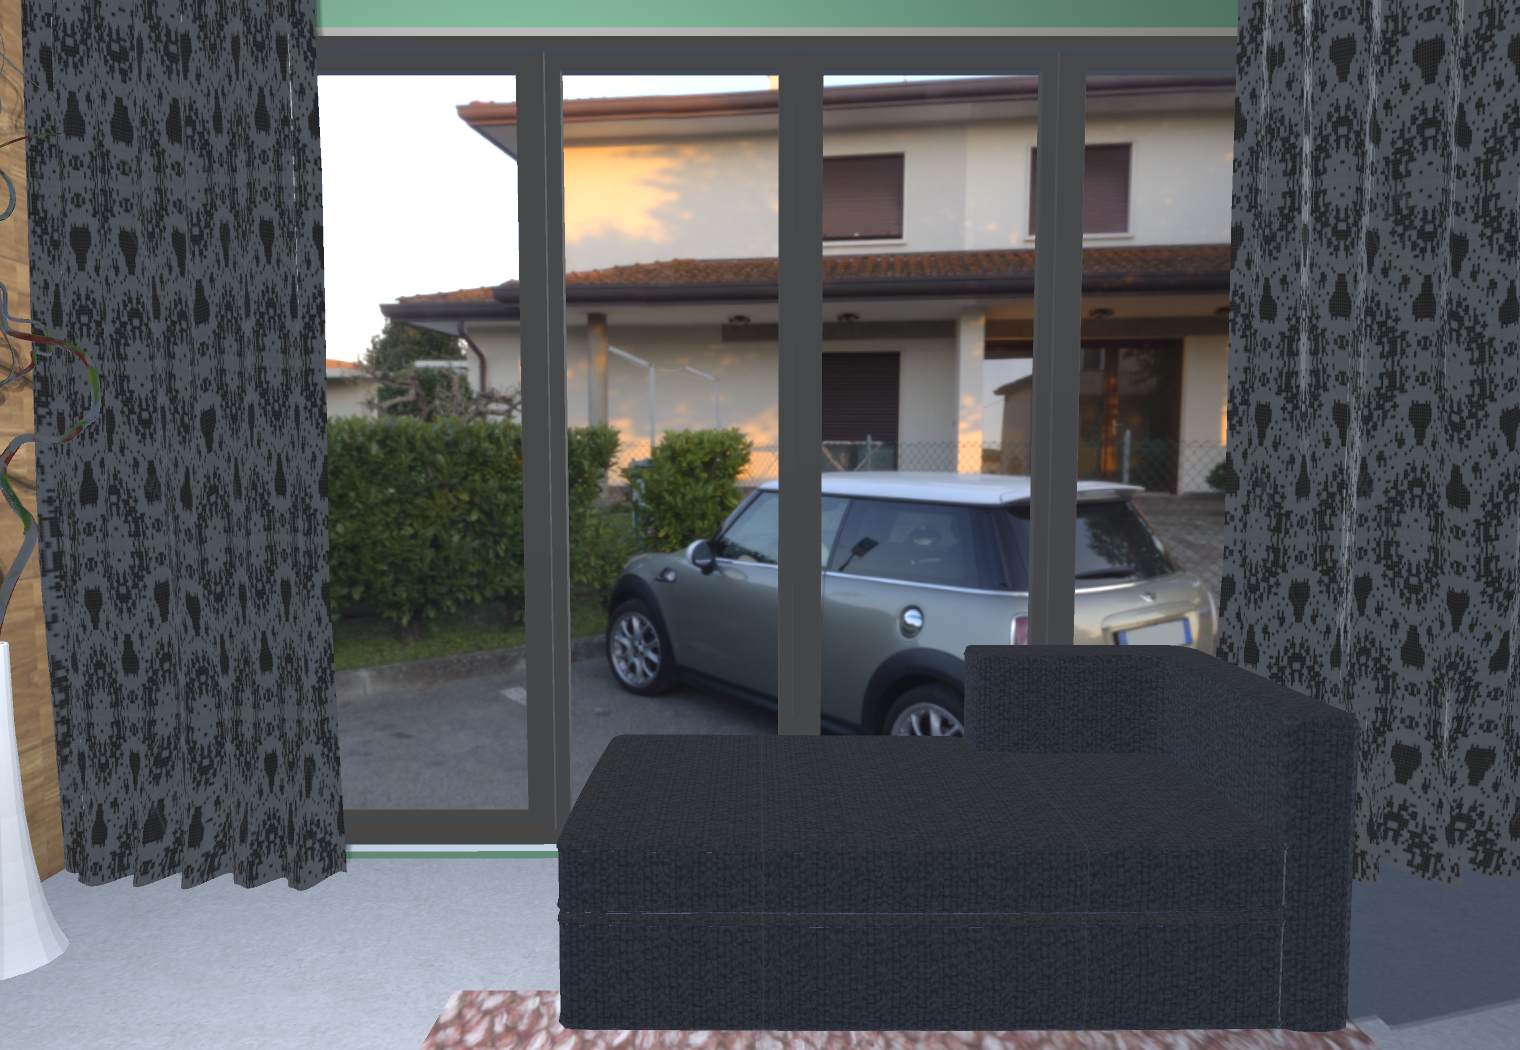
\includegraphics[width=.4\textwidth, height = .3\textwidth,valign=m]{/Users/apple/OVGU/Thesis/code/3dReconstruction/report/images/implementation/randomisation/skybox_1}
    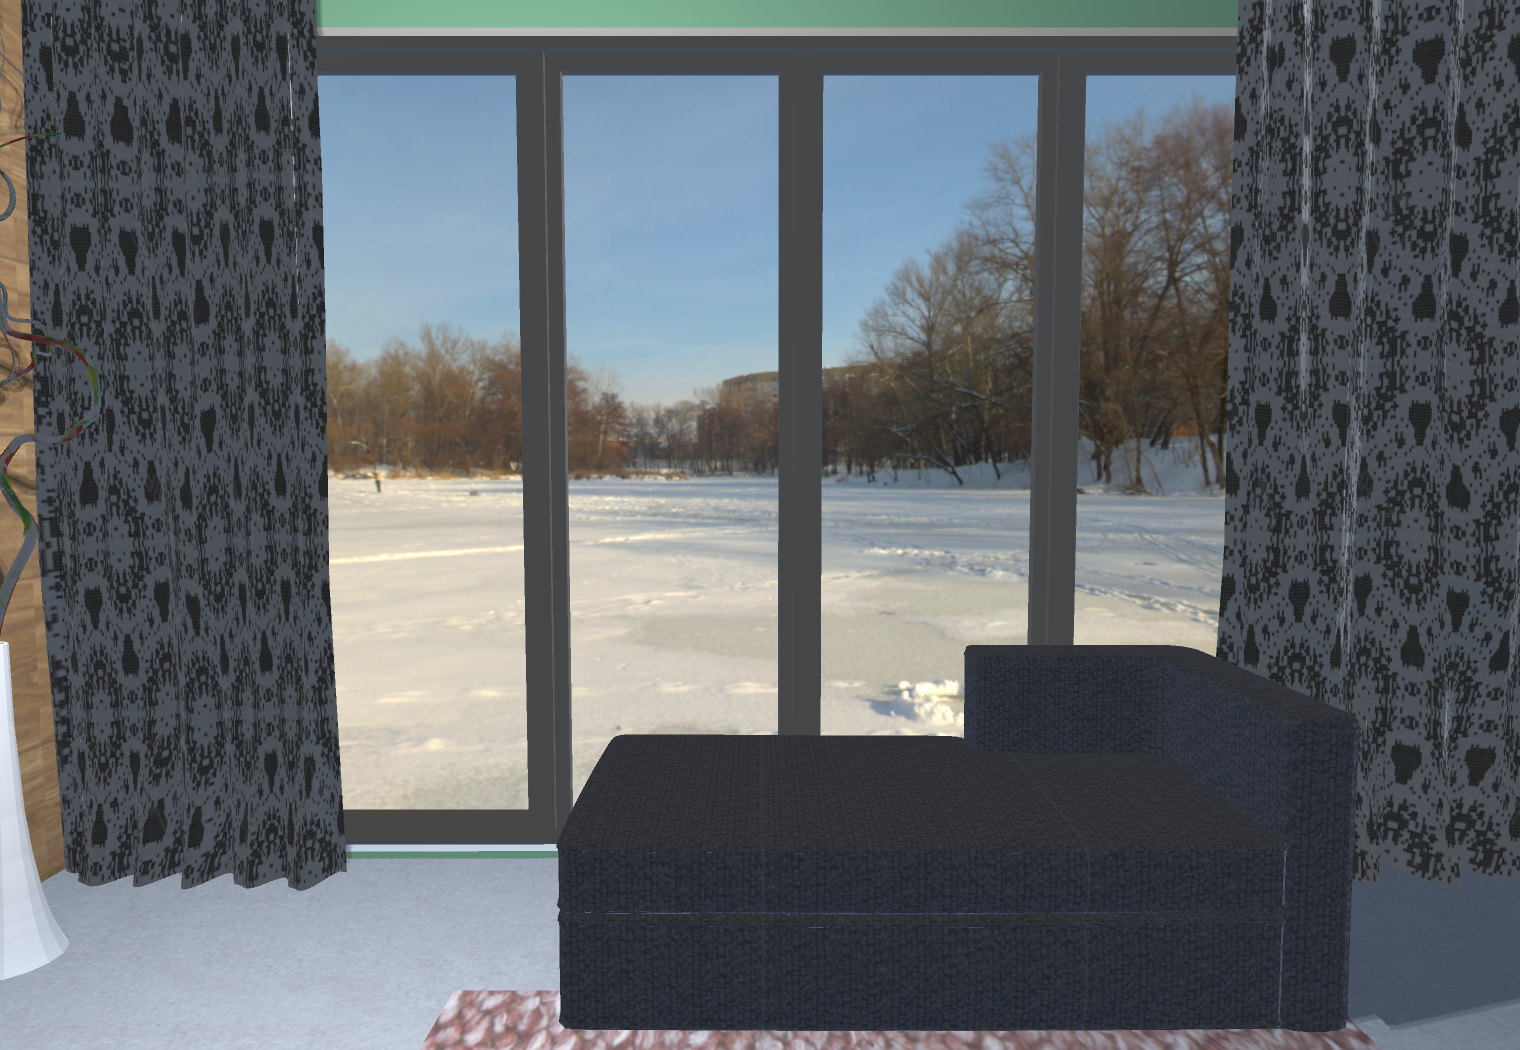
\includegraphics[width=.4\textwidth, height = .3\textwidth,valign=m]{/Users/apple/OVGU/Thesis/code/3dReconstruction/report/images/implementation/randomisation/skybox_2} \\
    \vspace{0.1cm}
    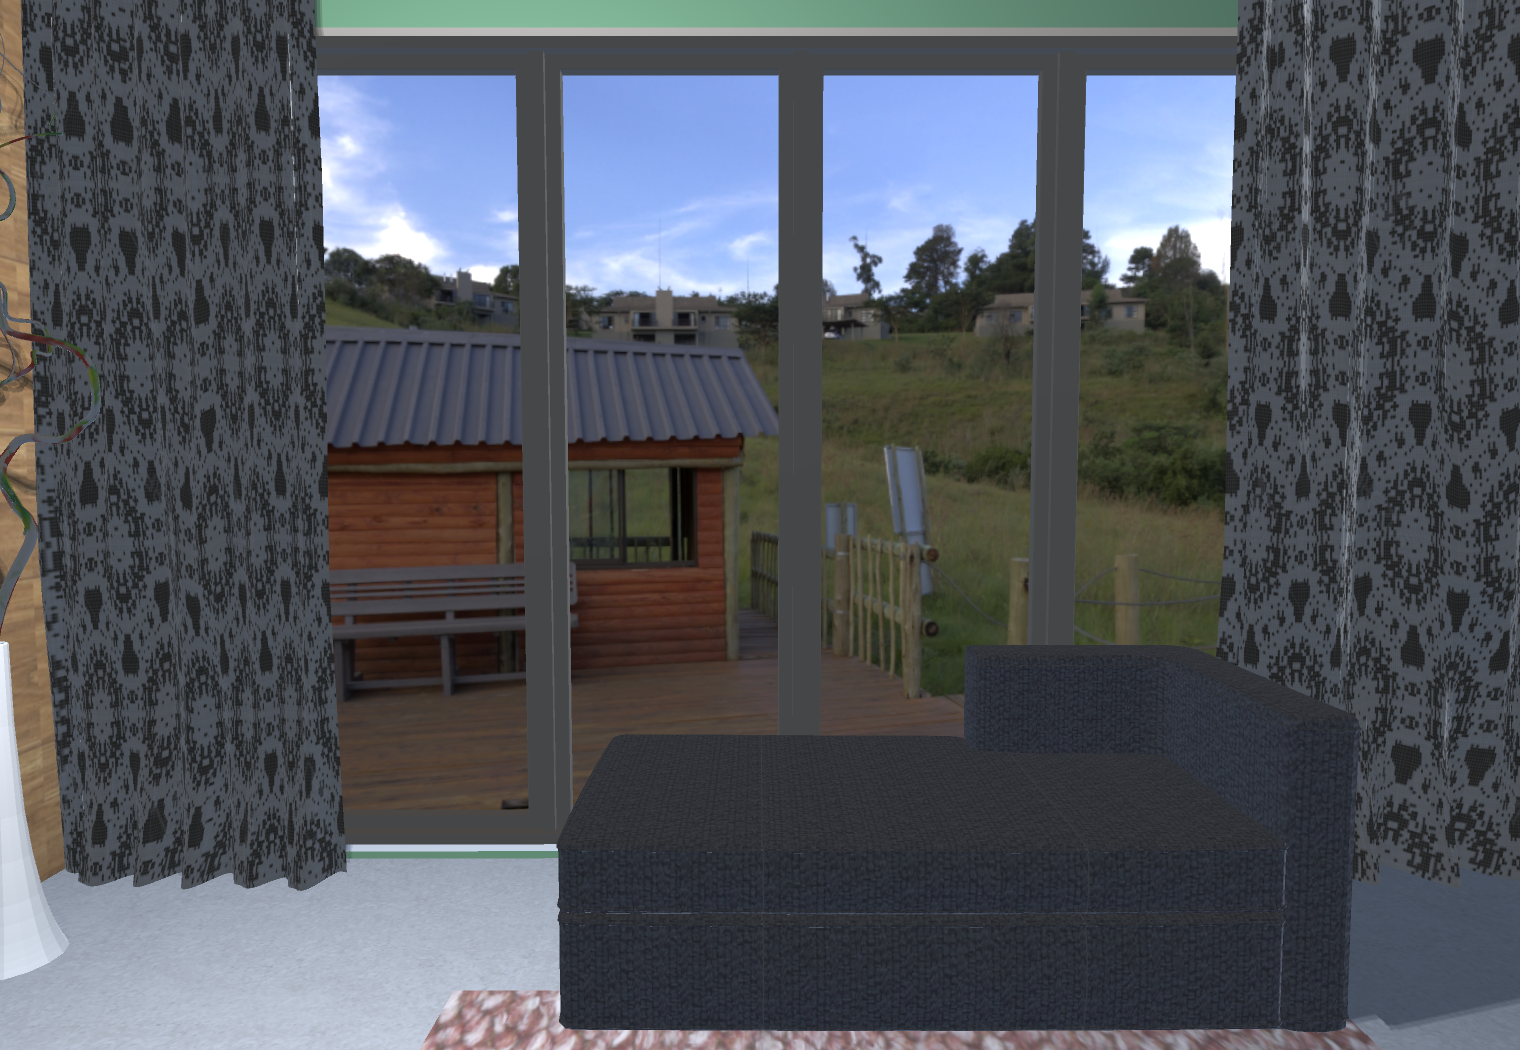
\includegraphics[width=.4\textwidth, height = .3\textwidth,valign=m]{/Users/apple/OVGU/Thesis/code/3dReconstruction/report/images/implementation/randomisation/skybox_3}
    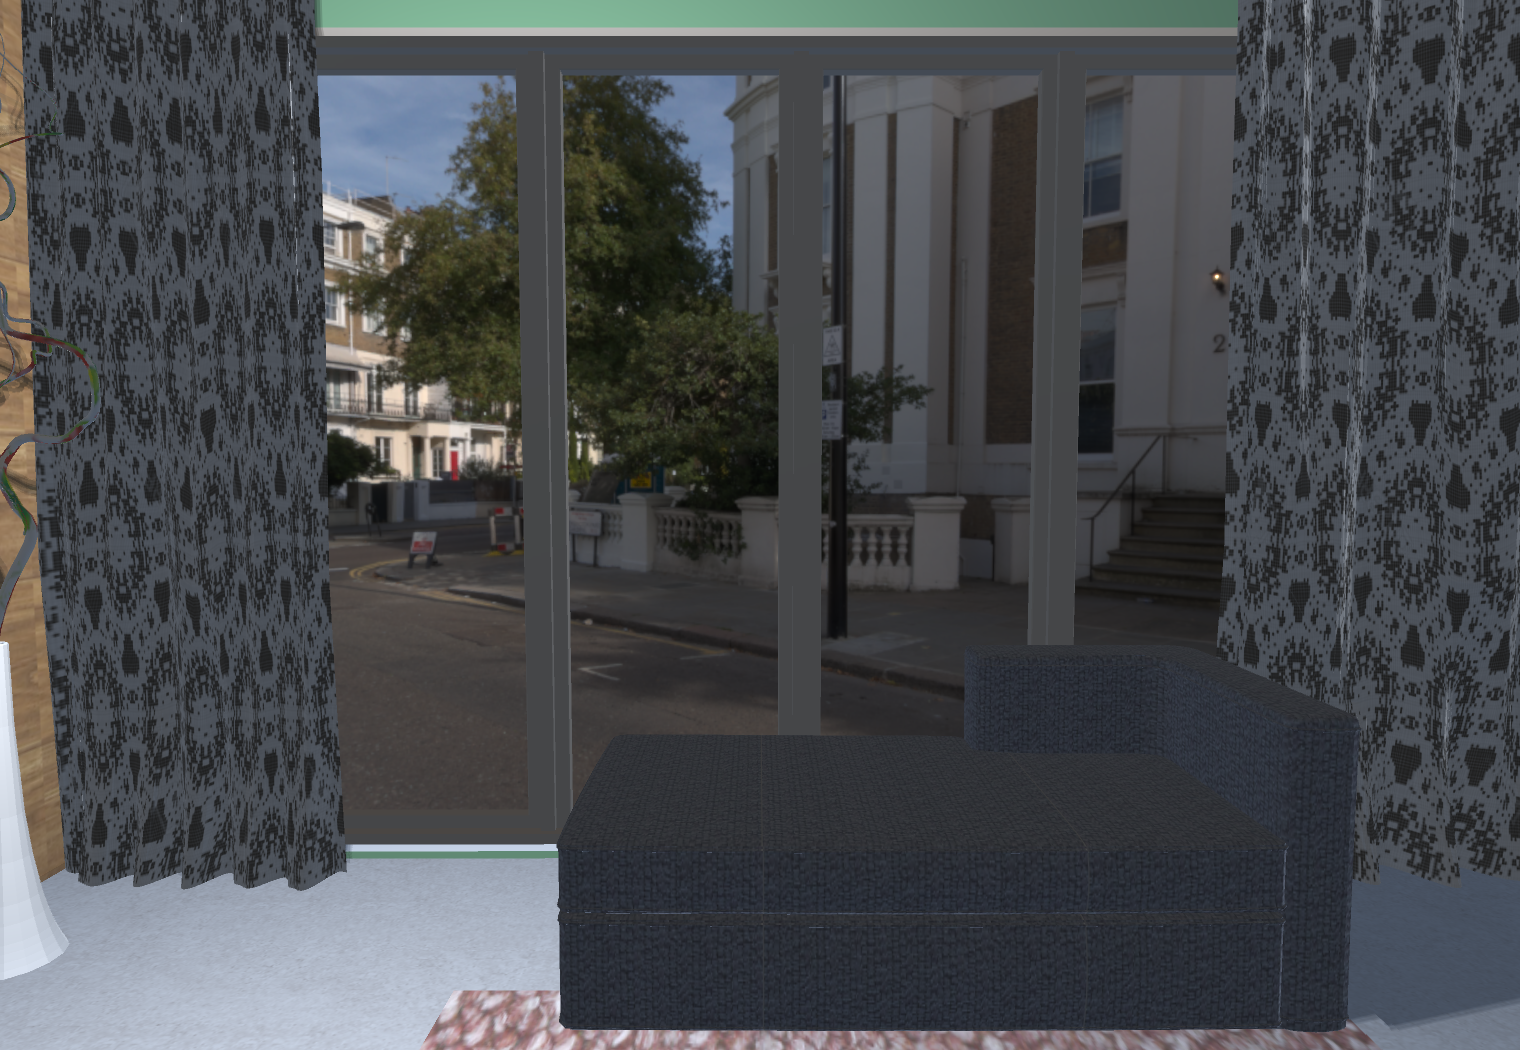
\includegraphics[width=.4\textwidth, height = .3\textwidth,valign=m]{/Users/apple/OVGU/Thesis/code/3dReconstruction/report/images/implementation/randomisation/skybox_4}\\
    \caption[Samples for Skyboxes.]{Samples for different skyboxes which change the outdoor environment for the scenes. In the figure we see an open window with changing skybox.}
    \label{fig:skybox samples}
\end{figure}



\subsection{Replacing Target Objects}\label{subsec:replacing-target-objects}

To further randomize the scene, the category of target objects is replaced by the object under observation.
When more than one object of the same category is present, we randomize the object to be replaced, further randomizing the captured data.
The target object is scaled such that the least dimension of the target object matches the least dimension of the category object in the scene.
For example, if the length of the category object in the scene is the most petite amount length, width, and height, then the target object is scaled to match this length.
The rescaling makes the target object blend in with the scene.
Samples for replacing a target object from an original scene from Scenenet are shown in \autoref{fig:replace model}.

\begin{figure}
    \centering
    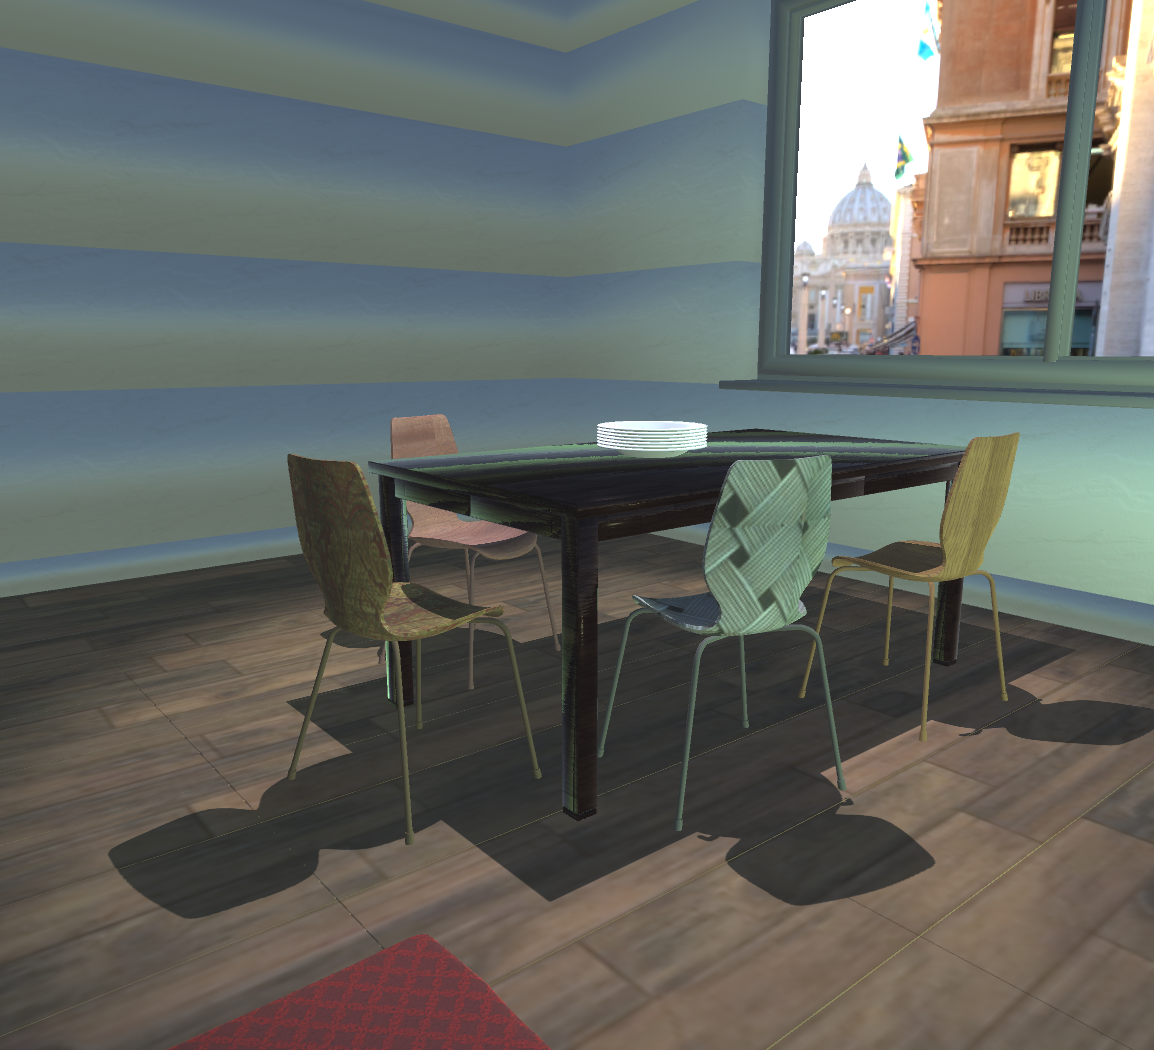
\includegraphics[width=.4\textwidth, height = .3\textwidth,valign=m]{/Users/apple/OVGU/Thesis/code/3dReconstruction/report/images/implementation/randomisation/replace_1-1}
    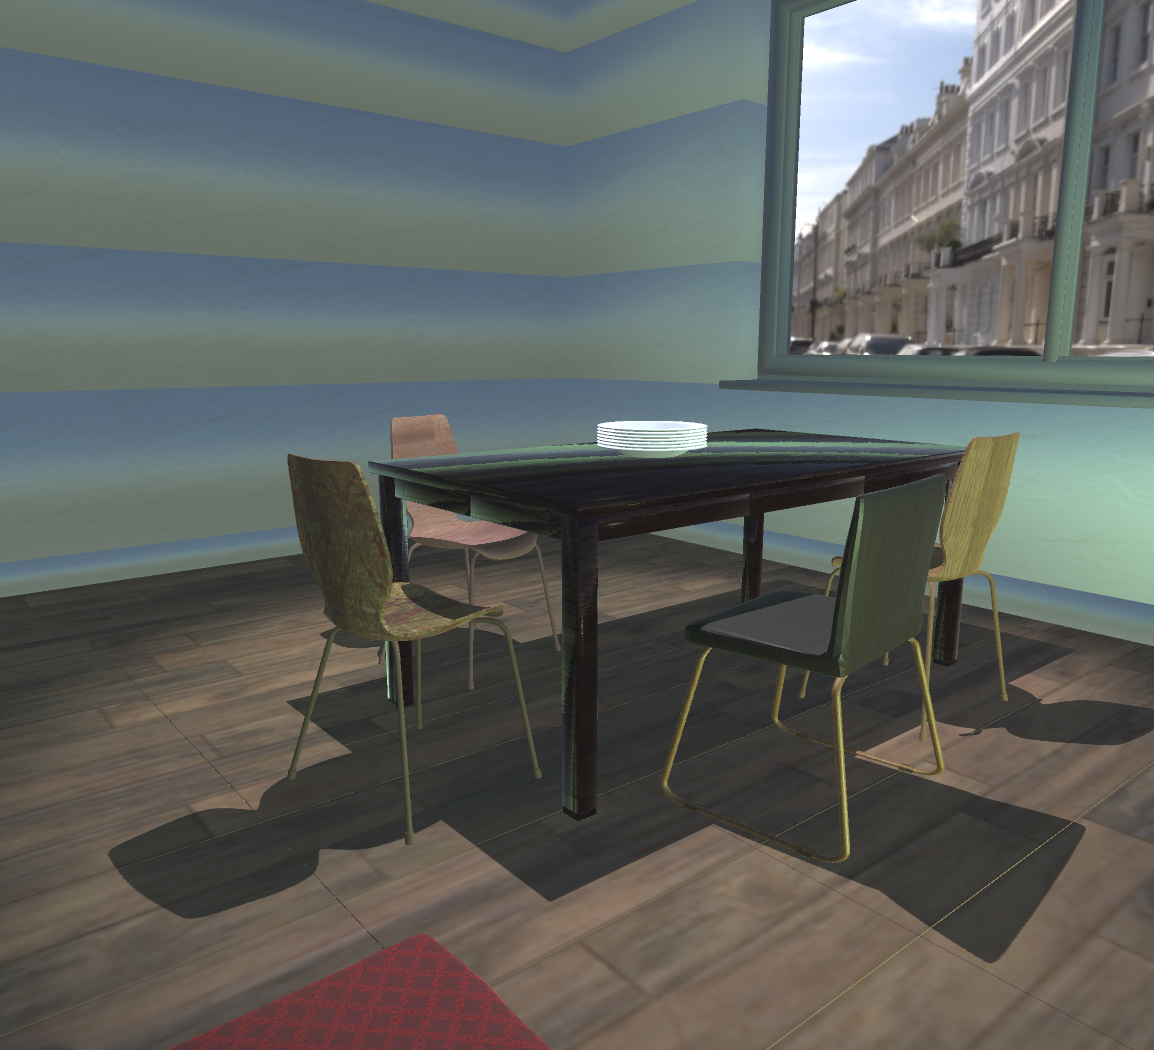
\includegraphics[width=.4\textwidth, height = .3\textwidth,valign=m]{/Users/apple/OVGU/Thesis/code/3dReconstruction/report/images/implementation/randomisation/replace_1-2} \\
    \vspace{0.1cm}
    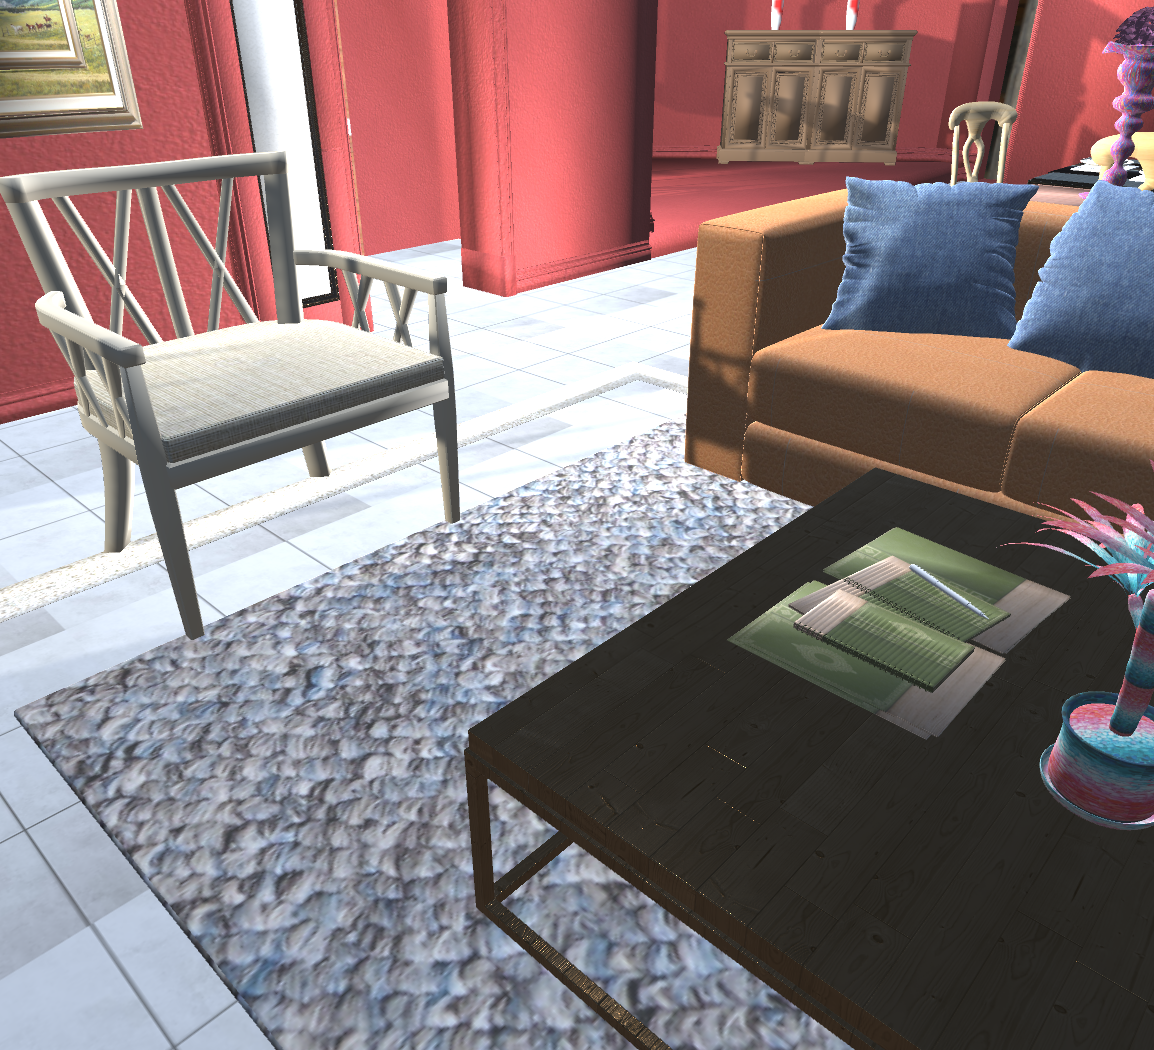
\includegraphics[width=.4\textwidth, height = .3\textwidth,valign=m]{/Users/apple/OVGU/Thesis/code/3dReconstruction/report/images/implementation/randomisation/replace_2-1}
    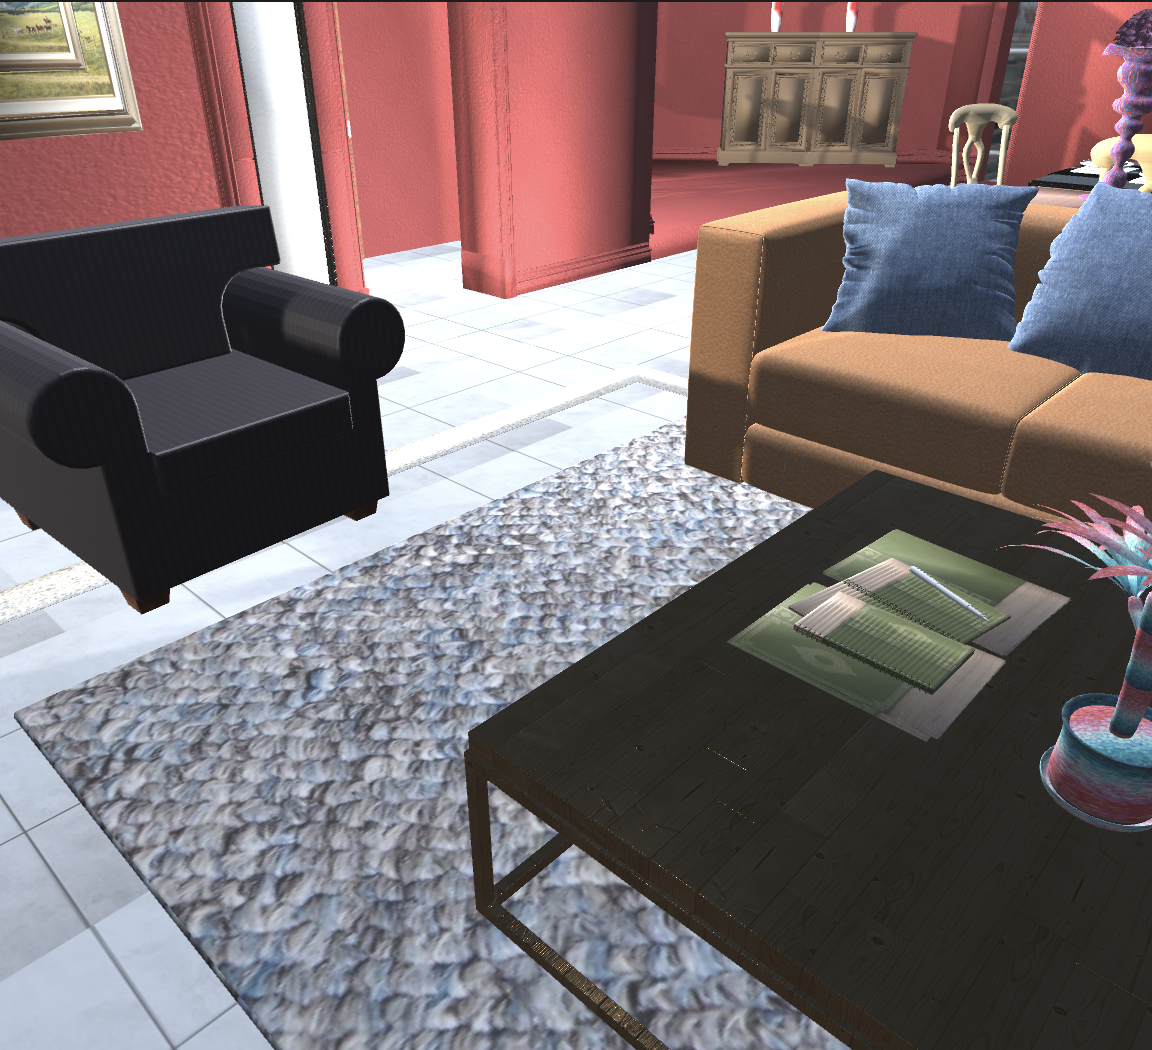
\includegraphics[width=.4\textwidth, height = .3\textwidth,valign=m]{/Users/apple/OVGU/Thesis/code/3dReconstruction/report/images/implementation/randomisation/replace_2-2}\\
    \caption[Samples for Object Replacement]{Samples for object replacement. The Left column shows a scene from SceneNet, while the right column shows an object being replaced in original scene.}
    \label{fig:replace model}
\end{figure}


\subsection{Camera ViewPoints}\label{subsec:camera-viewpoints}

We randomize camera position with some constraints such that we get different orientations of the target object with different backgrounds.
The constraints will include the height of the camera, minimum and maximum distance to the target object.
A random point is selected within this bound for the camera position.
We make sure that the target object is within the camera frame and is visible.
\autoref{fig:Camera viewpoints} shows samples of different camera viewpoints on a constant object and scene.

\begin{figure}
    \centering
    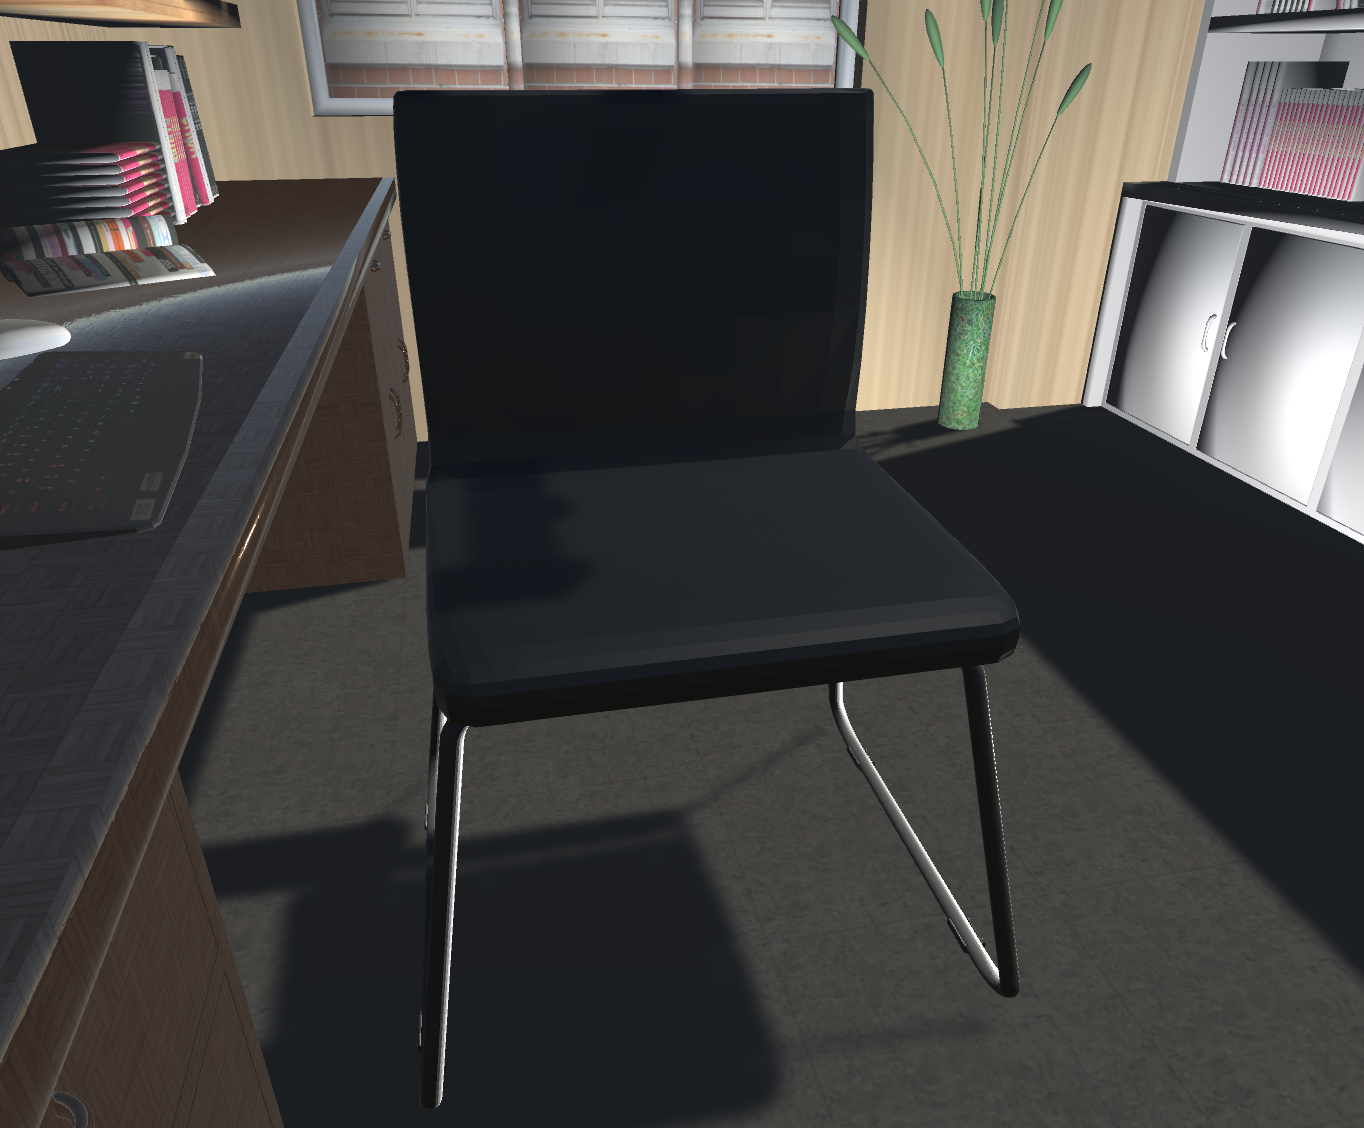
\includegraphics[width=.4\textwidth, height = .3\textwidth,valign=m]{/Users/apple/OVGU/Thesis/code/3dReconstruction/report/images/implementation/randomisation/camera1}
    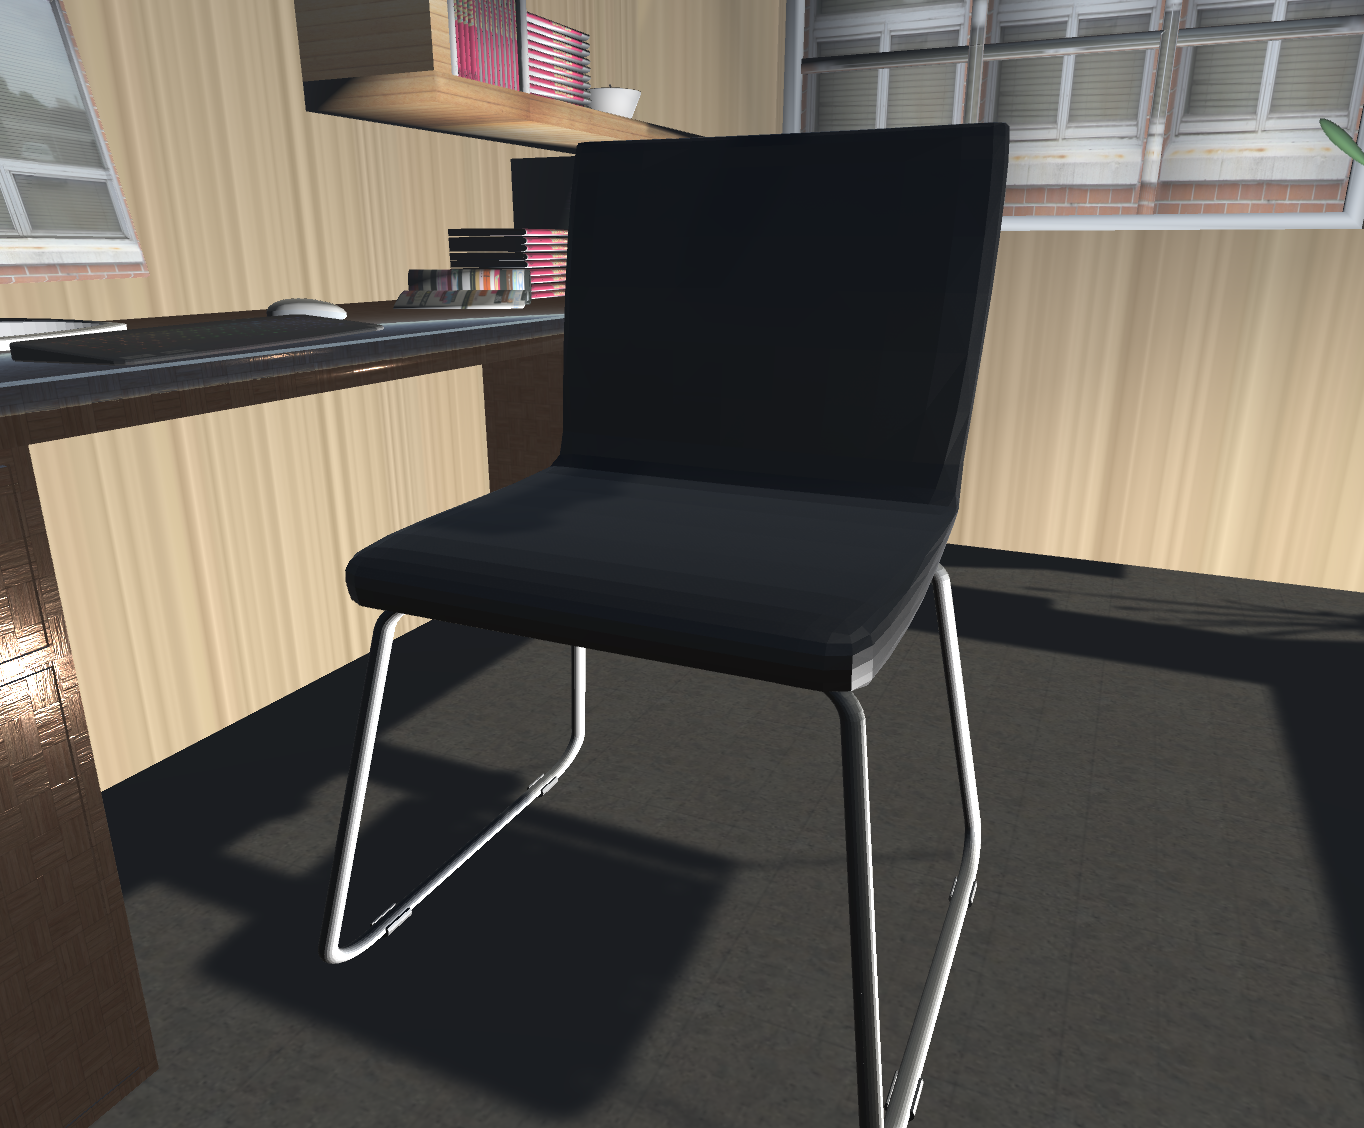
\includegraphics[width=.4\textwidth, height = .3\textwidth,valign=m]{/Users/apple/OVGU/Thesis/code/3dReconstruction/report/images/implementation/randomisation/camera2}\\
    \vspace{0.1cm}
    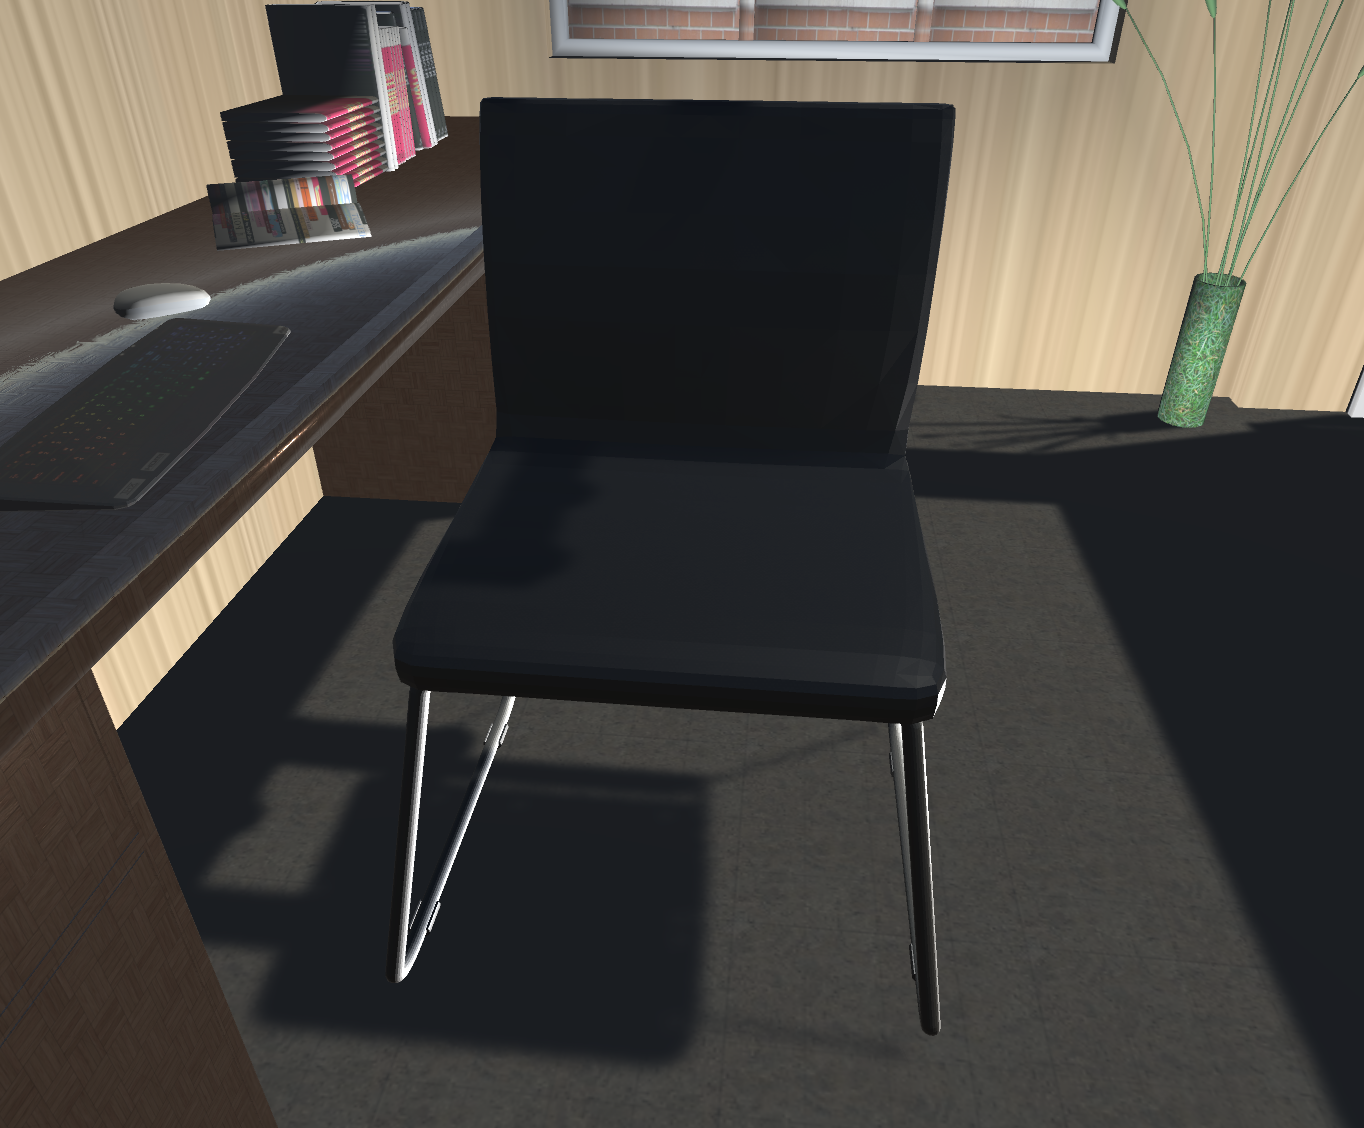
\includegraphics[width=.4\textwidth, height = .3\textwidth,valign=m]{/Users/apple/OVGU/Thesis/code/3dReconstruction/report/images/implementation/randomisation/camera3}
    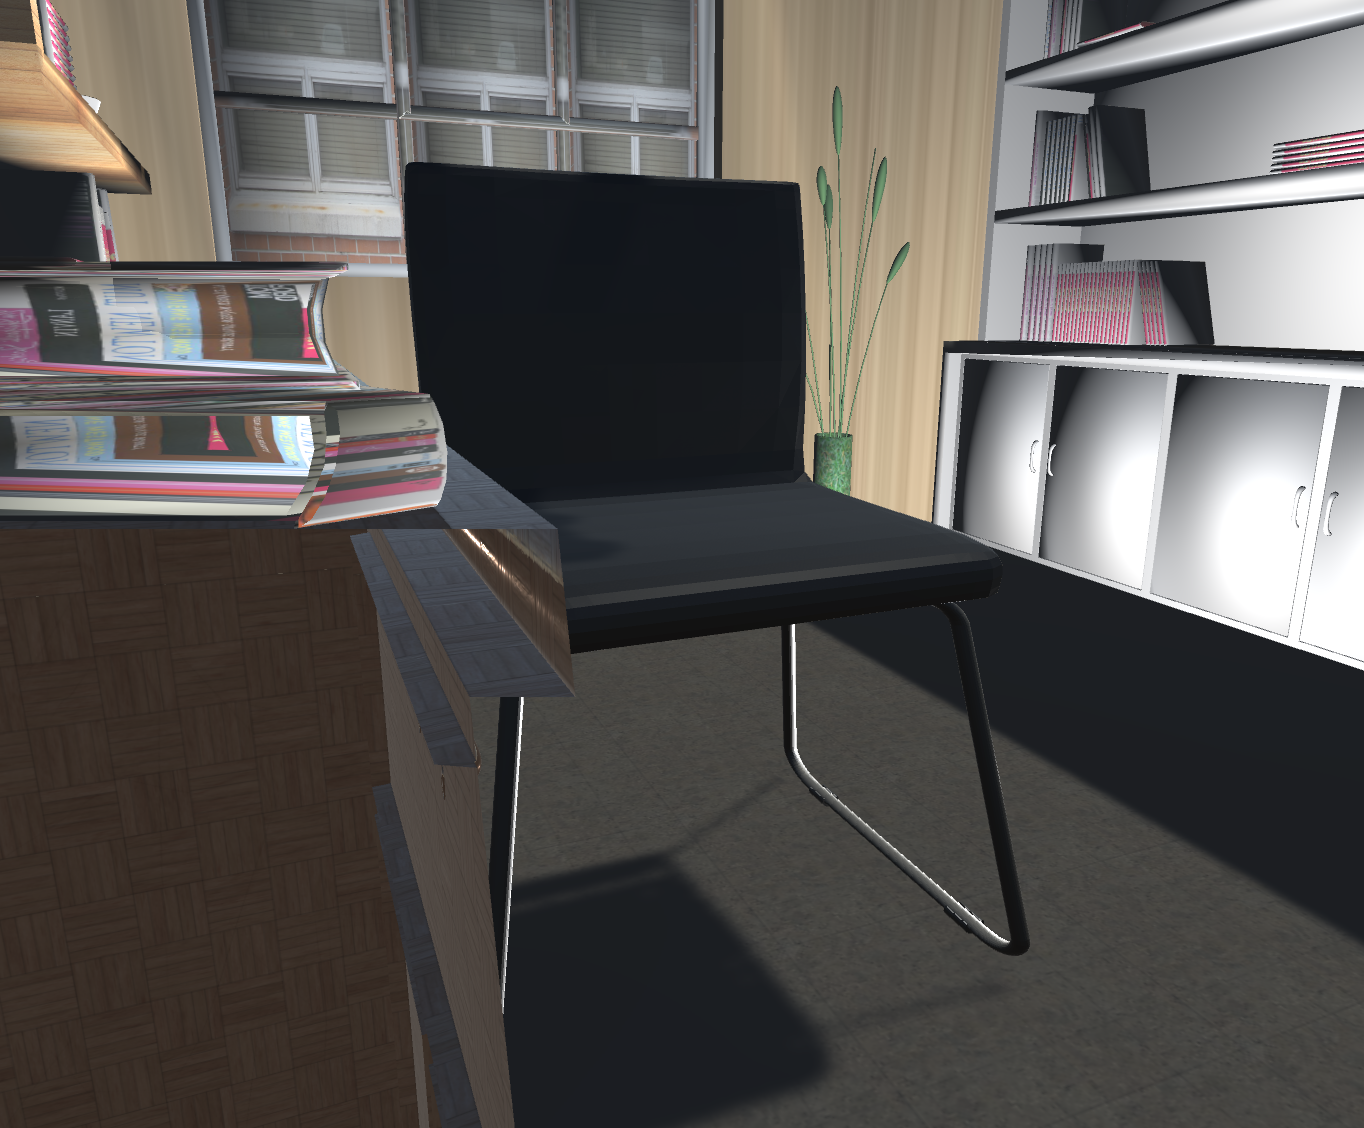
\includegraphics[width=.4\textwidth, height = .3\textwidth,valign=m]{/Users/apple/OVGU/Thesis/code/3dReconstruction/report/images/implementation/randomisation/camera4}\\
    \caption[Samples for Camera ViewPoints.]{Sample images with different camera viewpoints of same object with a constant scene.}
    \label{fig:Camera viewpoints}
\end{figure}

\subsection{Lightings and Shadows}\label{subsec:lightings-and-shadows}

Lighting plays a vital role in photorealism.
The shadows formed with different lighting conditions enhance the photorealism of the images.
Unity offers a wide variety of illumination like global light, which acts like sunlight, and various indoor lighting systems.
Ideally, we should make the luminous objects like lamps, chandeliers, bulbs, etc.,
the source of light for indoor scenes, but we observed that the room does not light up uniformly, making it less photorealistic.
Hence we use some pre-determined lighting settings, discussed further in implementation(Section 4.1).

%\begin{figure}
%    \centering
%    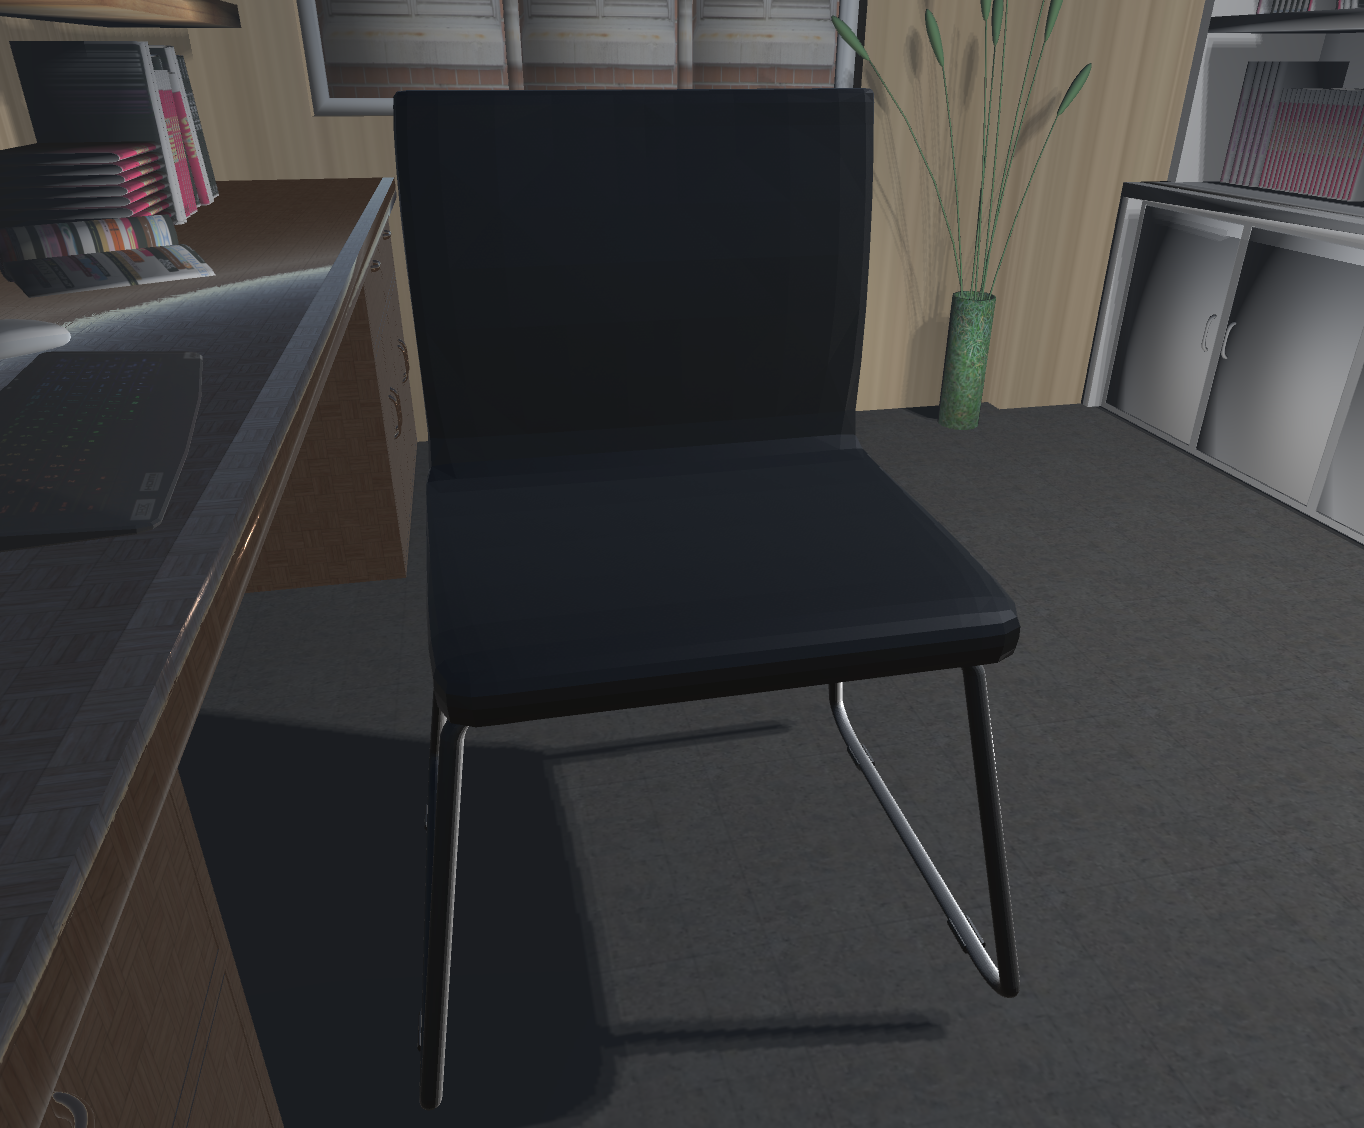
\includegraphics[width=.3\textwidth, height = .3\textwidth,valign=m]{/Users/apple/OVGU/Thesis/code/3dReconstruction/report/images/implementation/randomisation/lighting1}
%    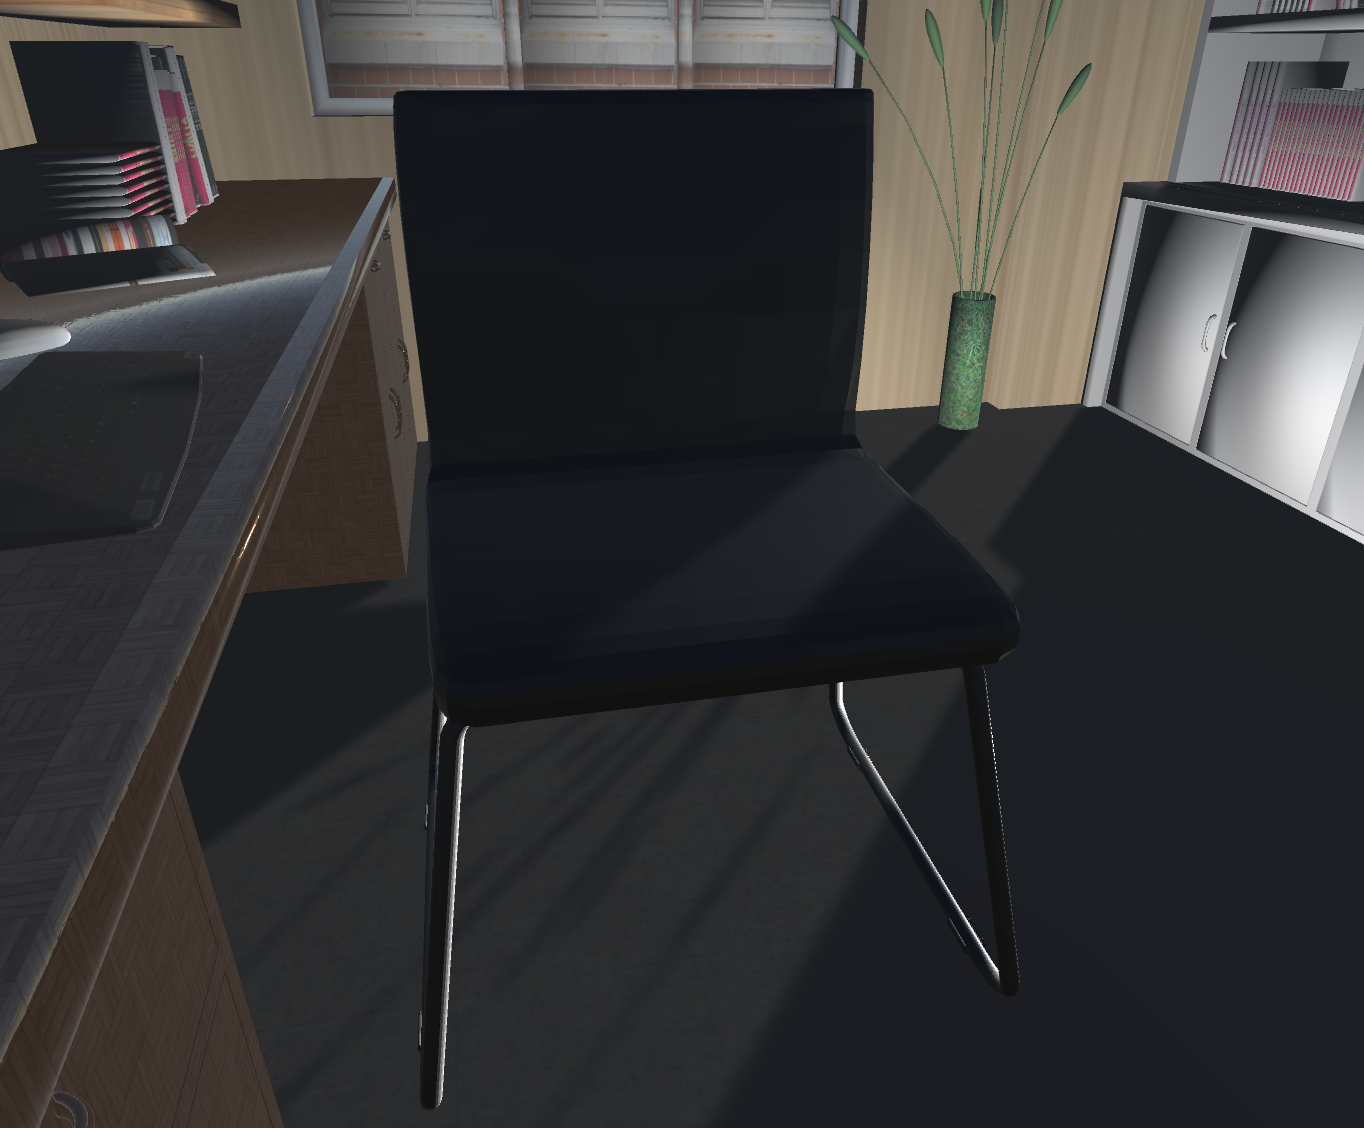
\includegraphics[width=.3\textwidth, height = .3\textwidth,valign=m]{/Users/apple/OVGU/Thesis/code/3dReconstruction/report/images/implementation/randomisation/lighting2}\\
%    \vspace{0.1cm}
%    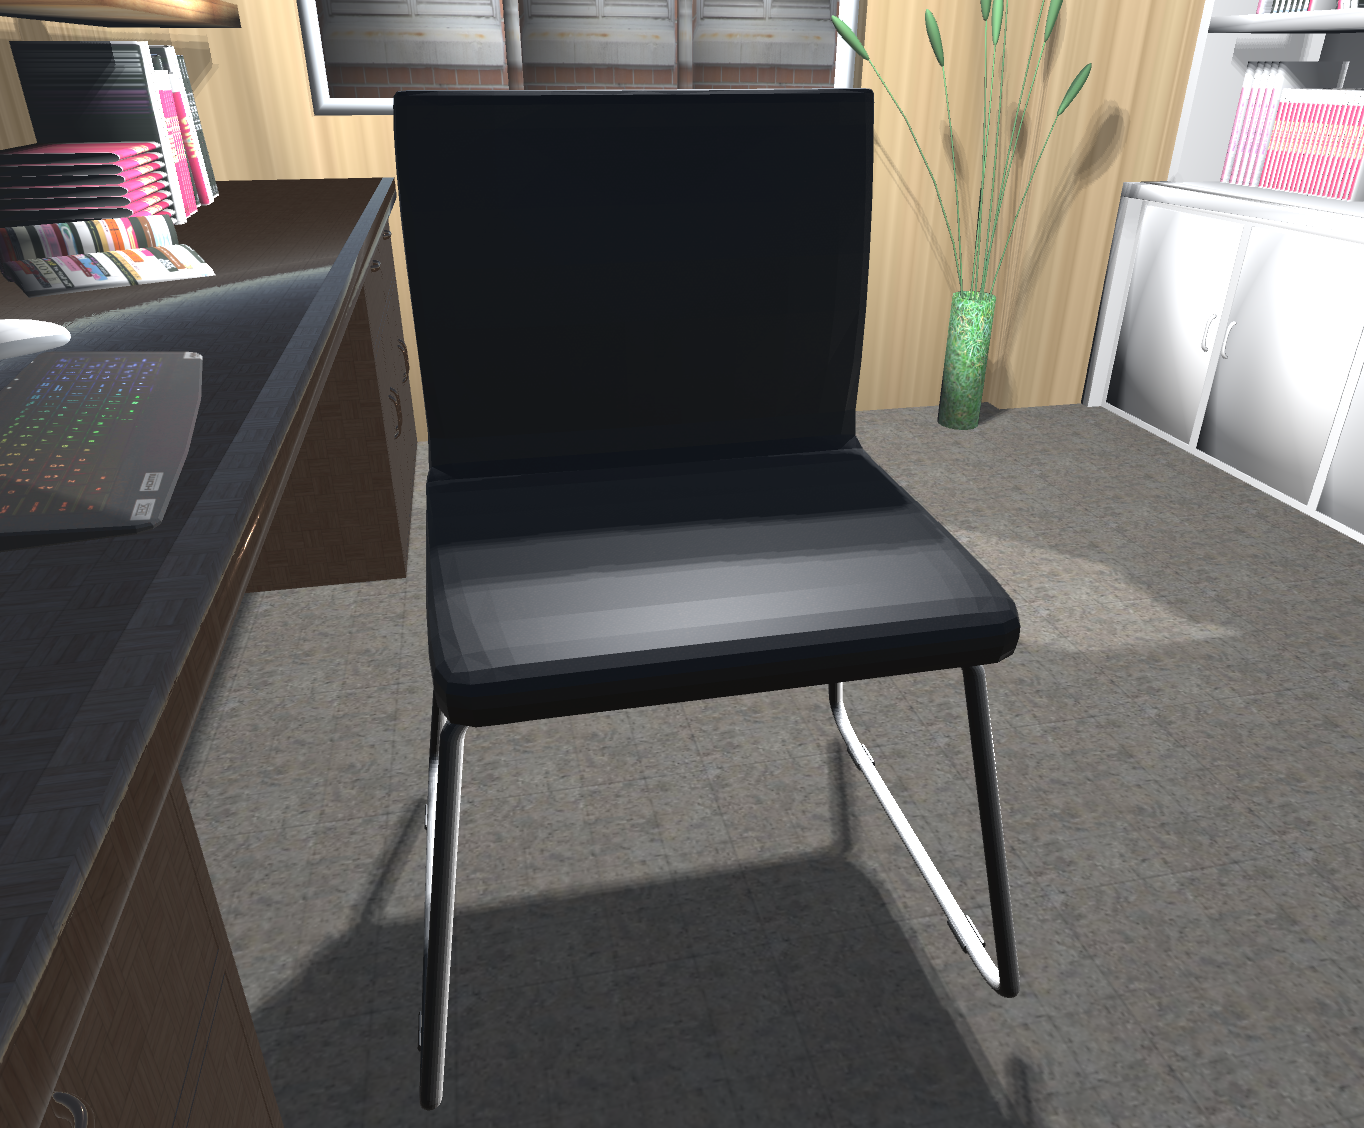
\includegraphics[width=.3\textwidth, height = .3\textwidth,valign=m]{/Users/apple/OVGU/Thesis/code/3dReconstruction/report/images/implementation/randomisation/lighting3}
%    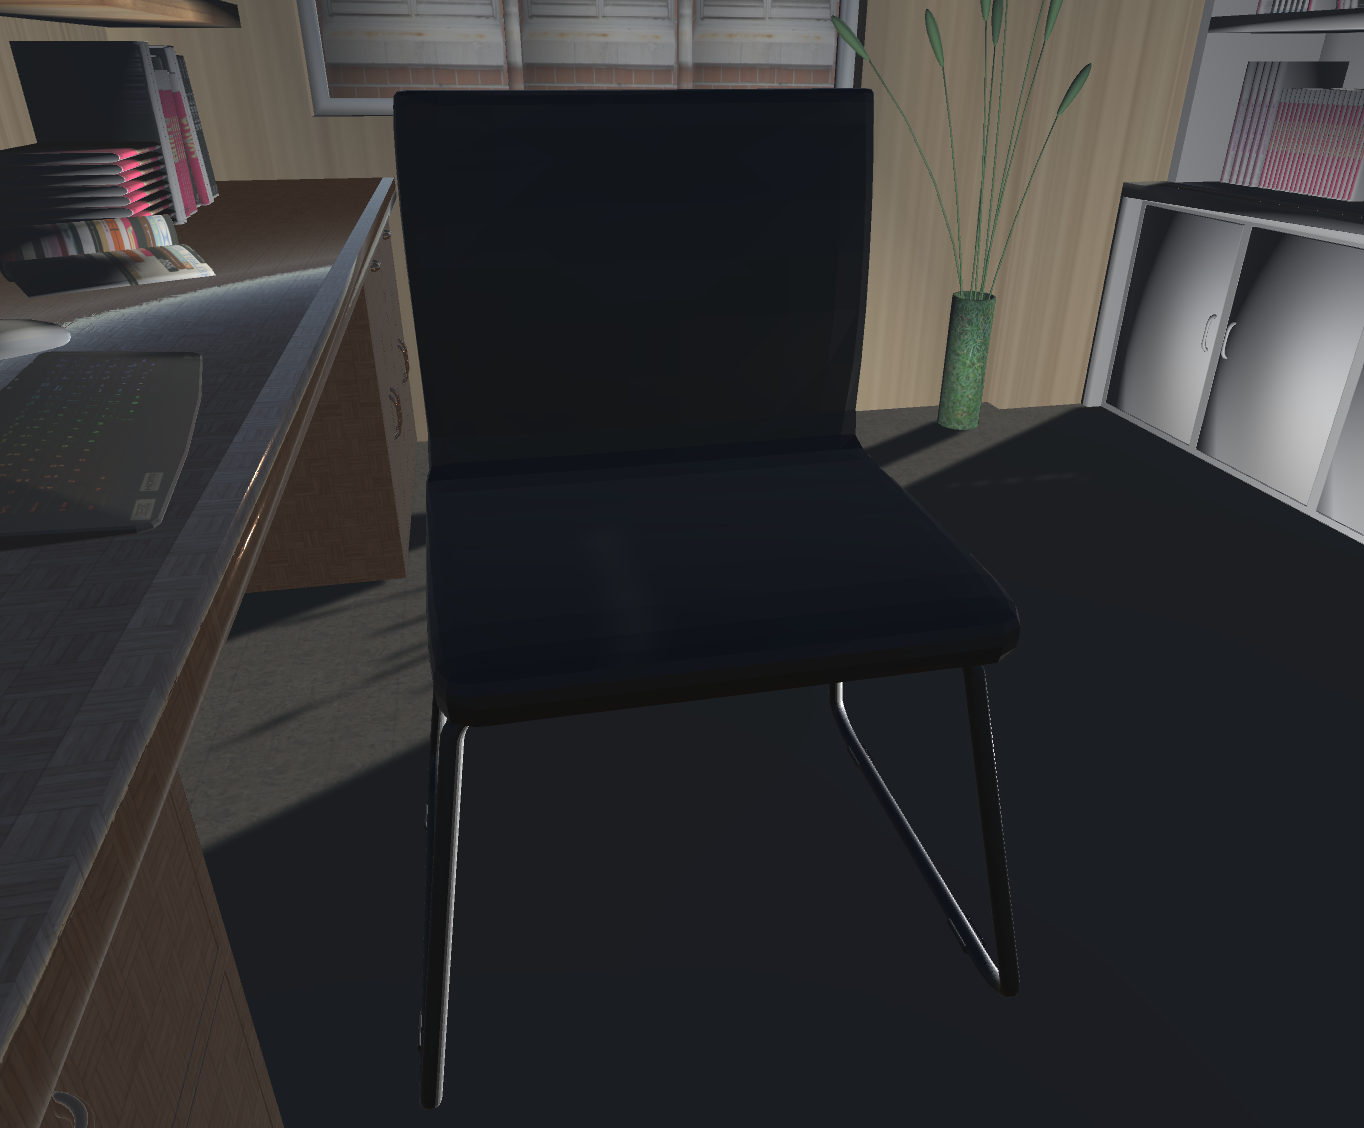
\includegraphics[width=.3\textwidth, height = .3\textwidth,valign=m]{/Users/apple/OVGU/Thesis/code/3dReconstruction/report/images/implementation/randomisation/lighting4}\\
%    \caption{Sample images with different lighting and shadows conditions}
%    \label{fig:Lighting and shadows}
%\end{figure}

\begin{figure}[ht]
    \centering
    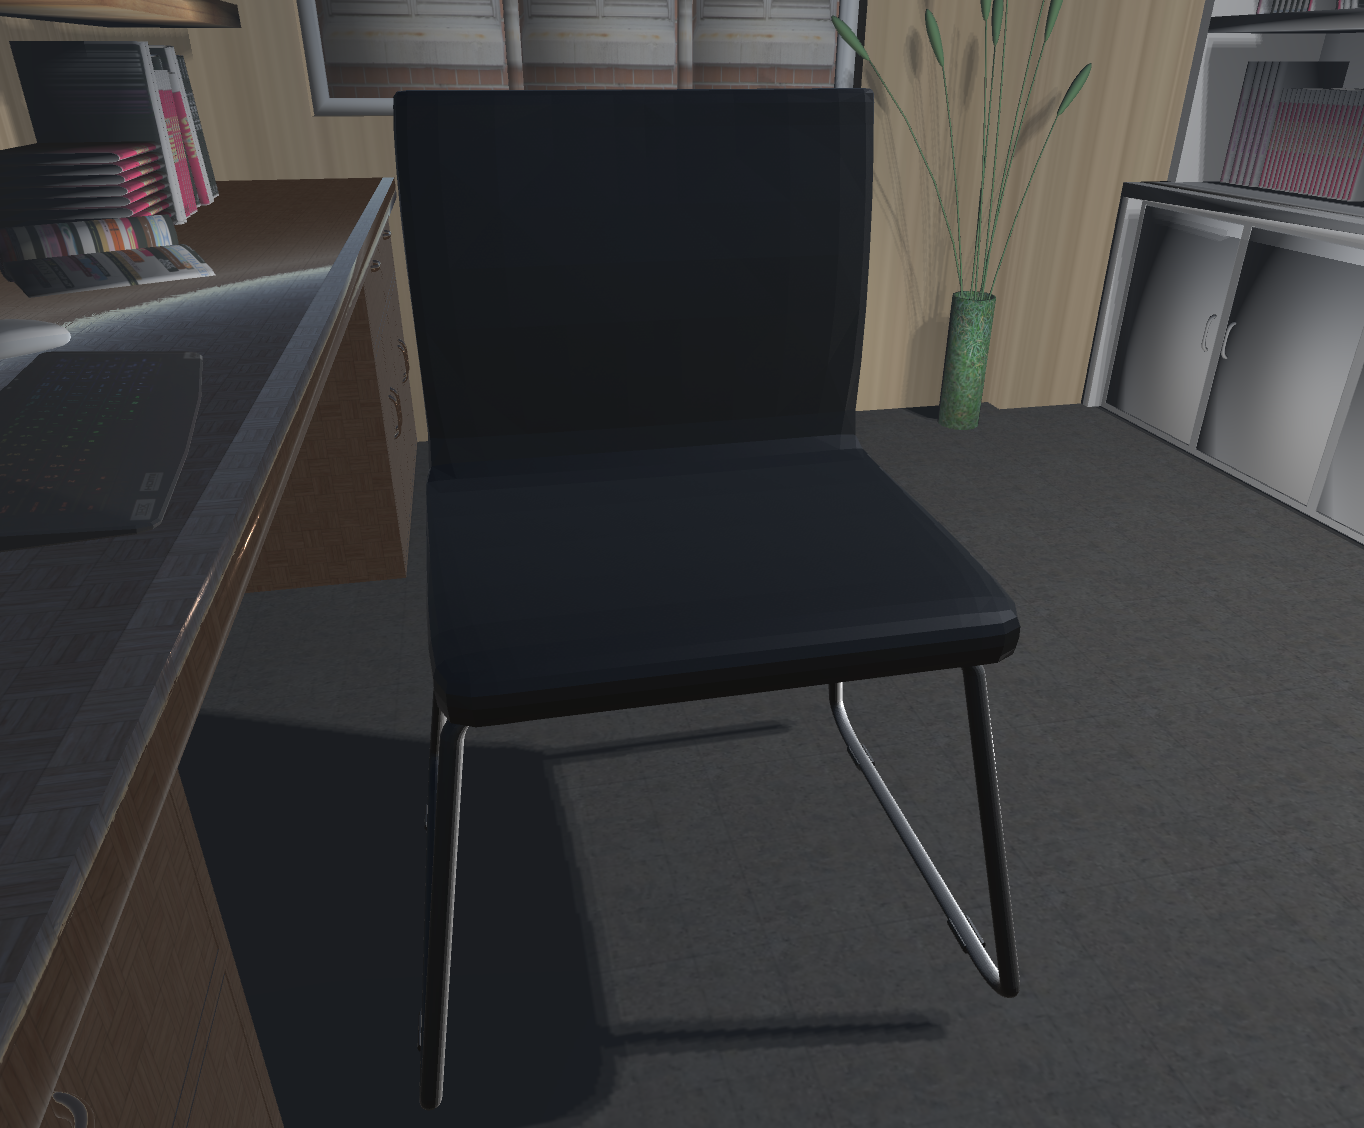
\includegraphics[width=.24\linewidth,valign=m]{/Users/apple/OVGU/Thesis/code/3dReconstruction/report/images/implementation/randomisation/lighting1}
    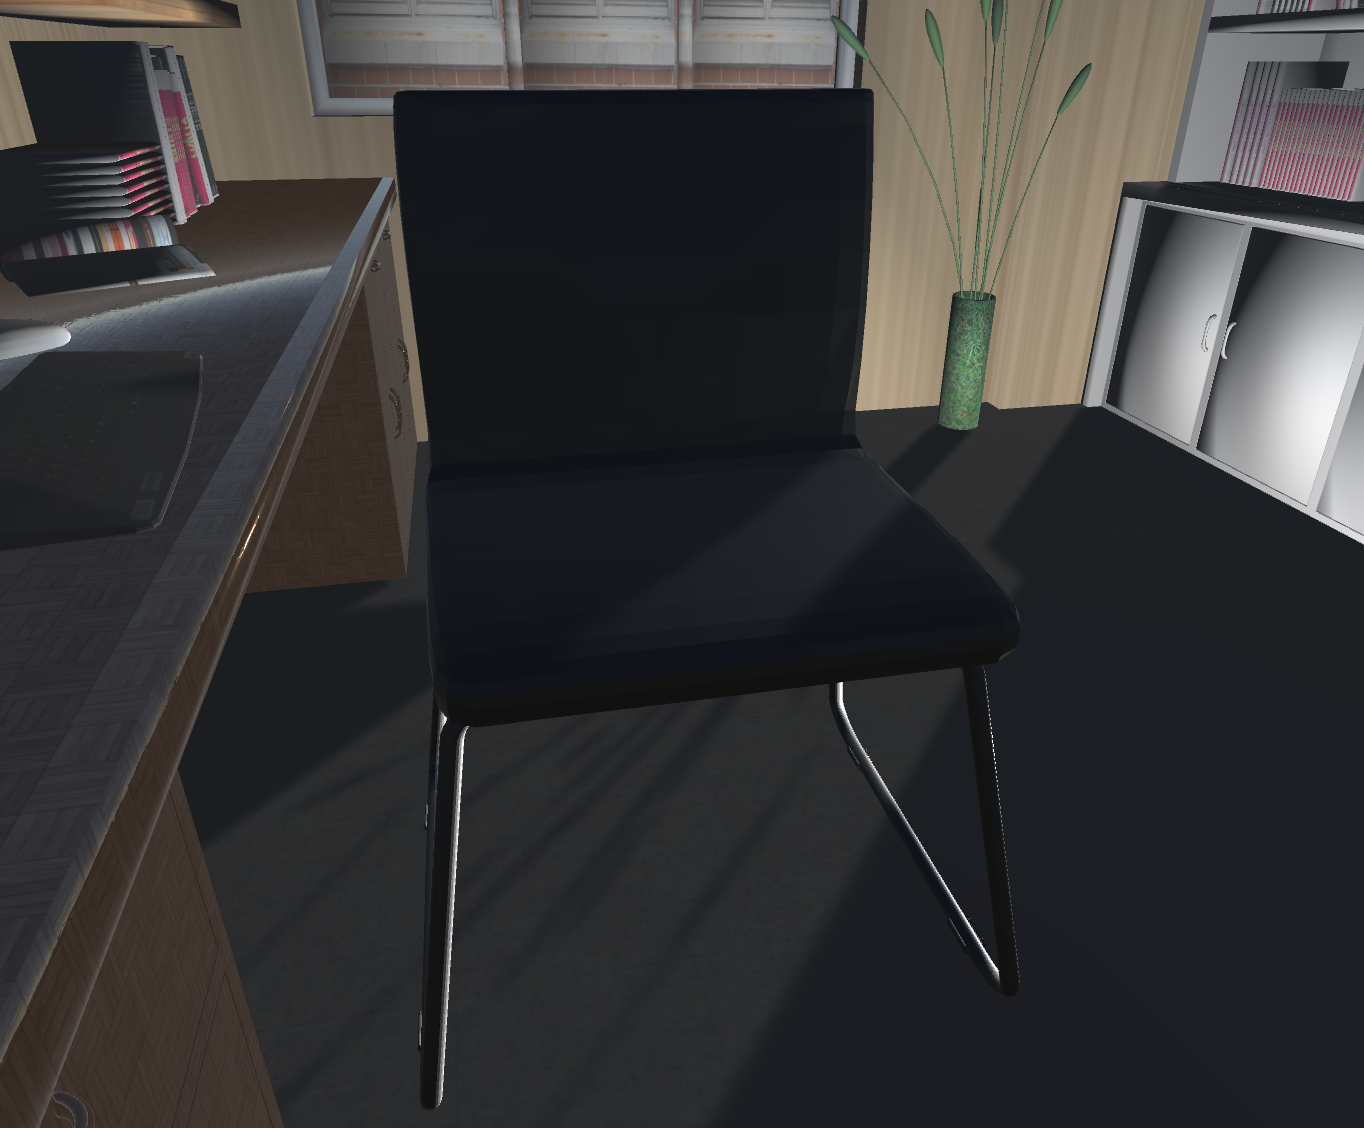
\includegraphics[width=.24\linewidth,valign=m]{/Users/apple/OVGU/Thesis/code/3dReconstruction/report/images/implementation/randomisation/lighting2}
    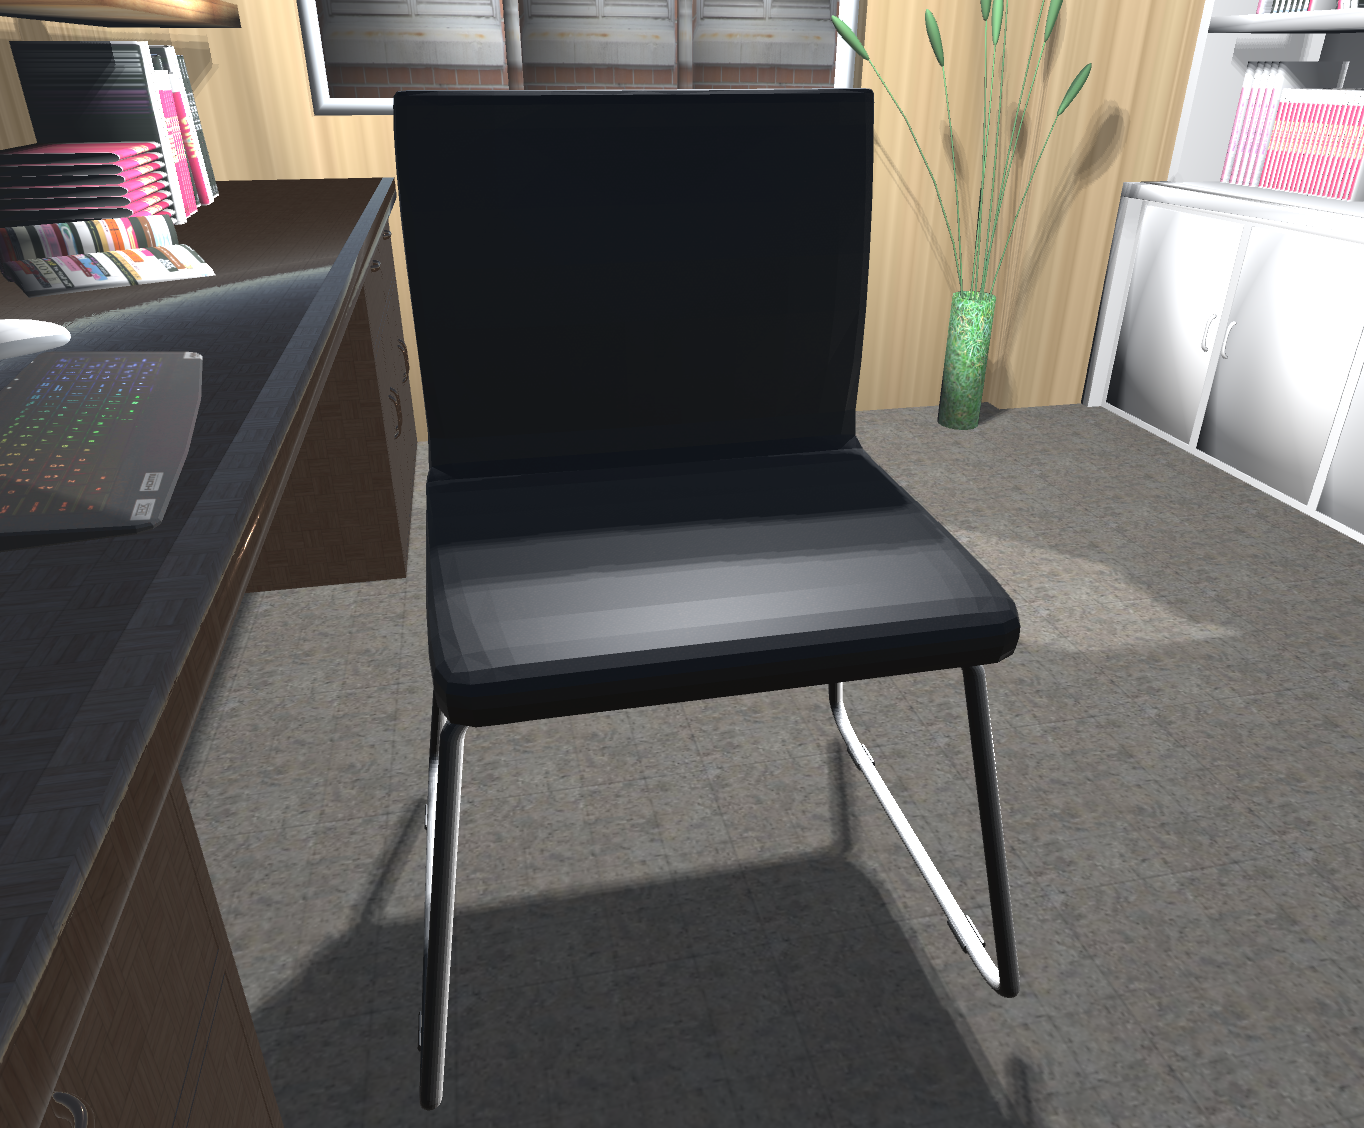
\includegraphics[width=.24\linewidth,valign=m]{/Users/apple/OVGU/Thesis/code/3dReconstruction/report/images/implementation/randomisation/lighting3}
    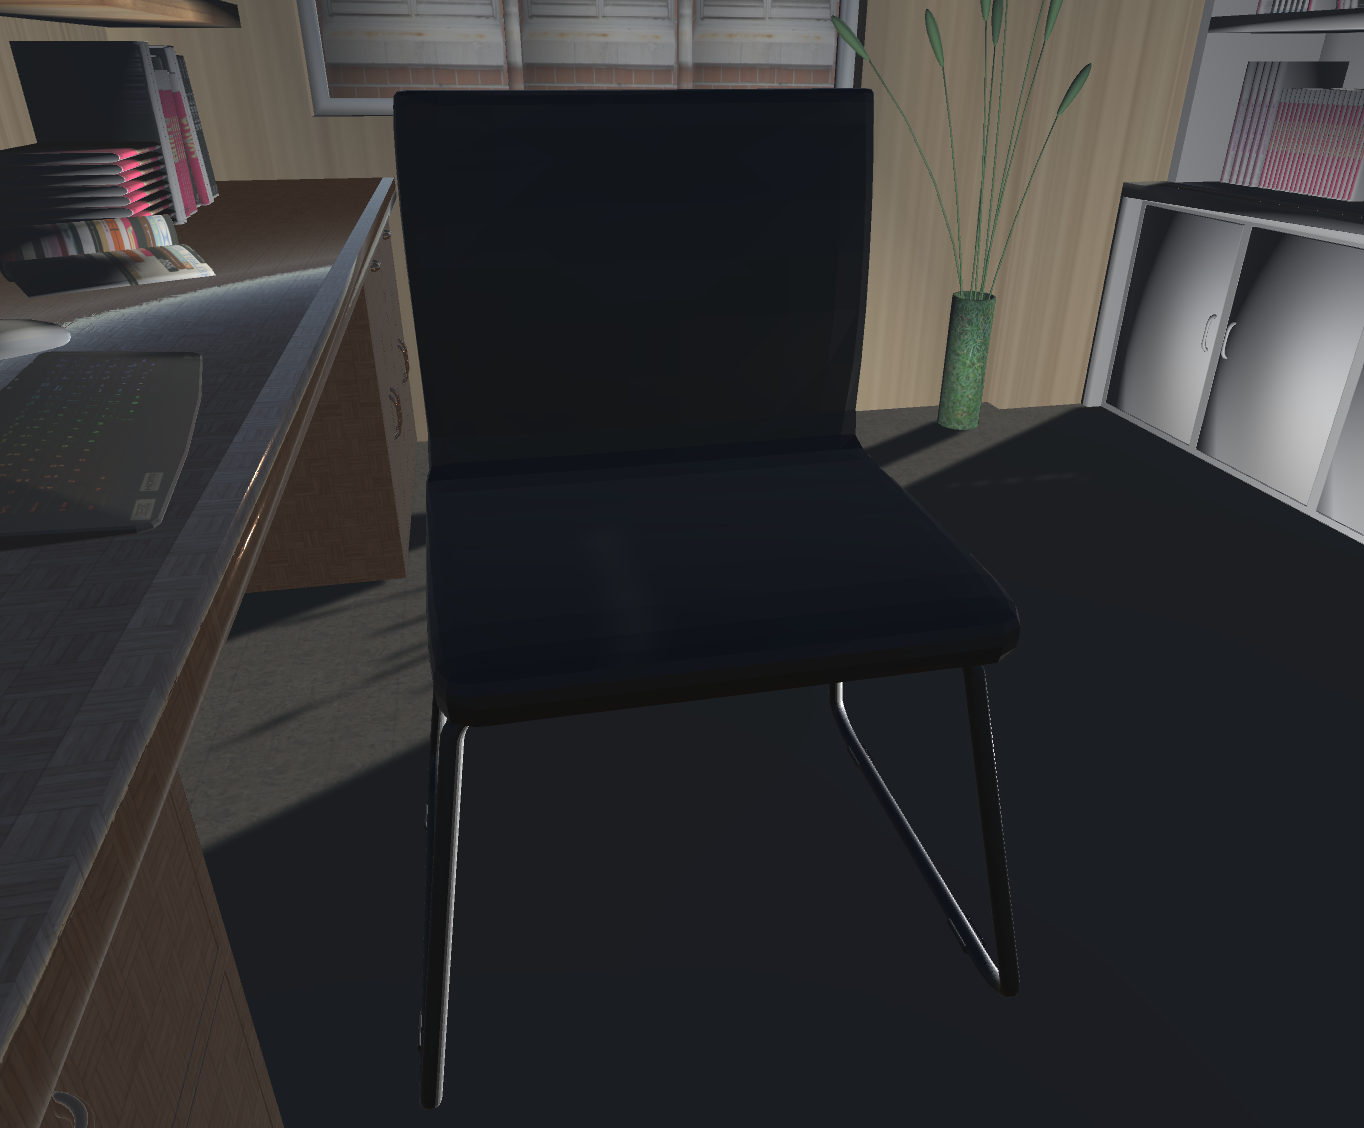
\includegraphics[width=.24\linewidth,valign=m]{/Users/apple/OVGU/Thesis/code/3dReconstruction/report/images/implementation/randomisation/lighting4}\\
    \vspace{0.1cm}
    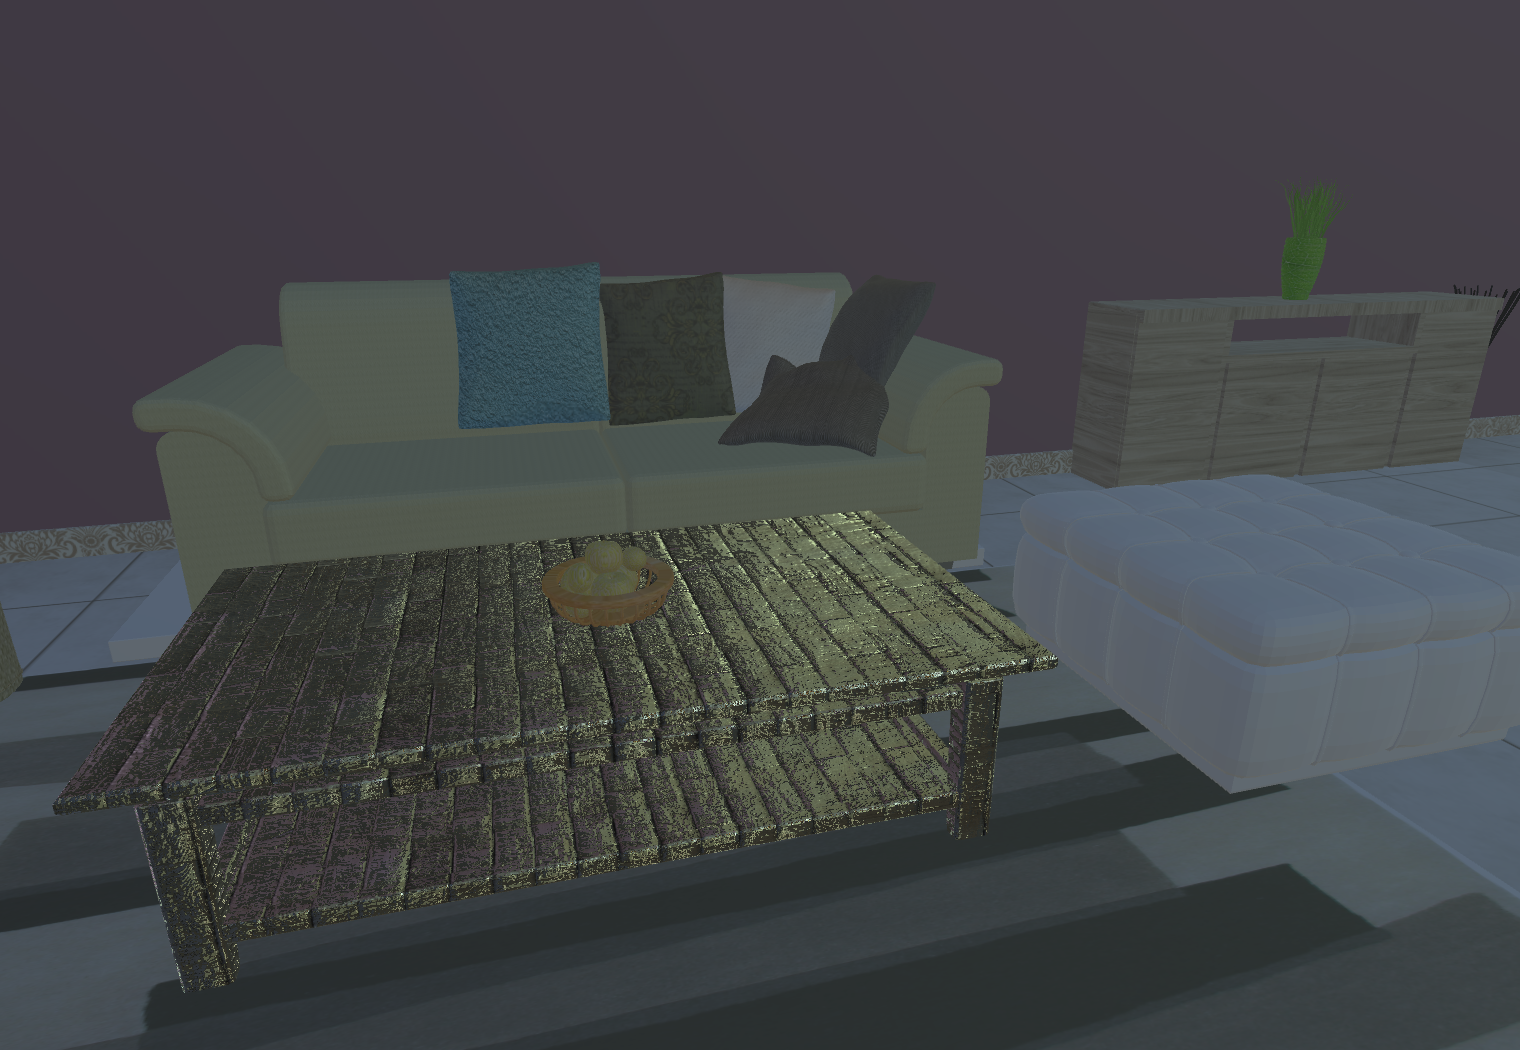
\includegraphics[width=.24\linewidth,valign=m]{/Users/apple/OVGU/Thesis/code/3dReconstruction/report/images/implementation/randomisation/lighting5}
    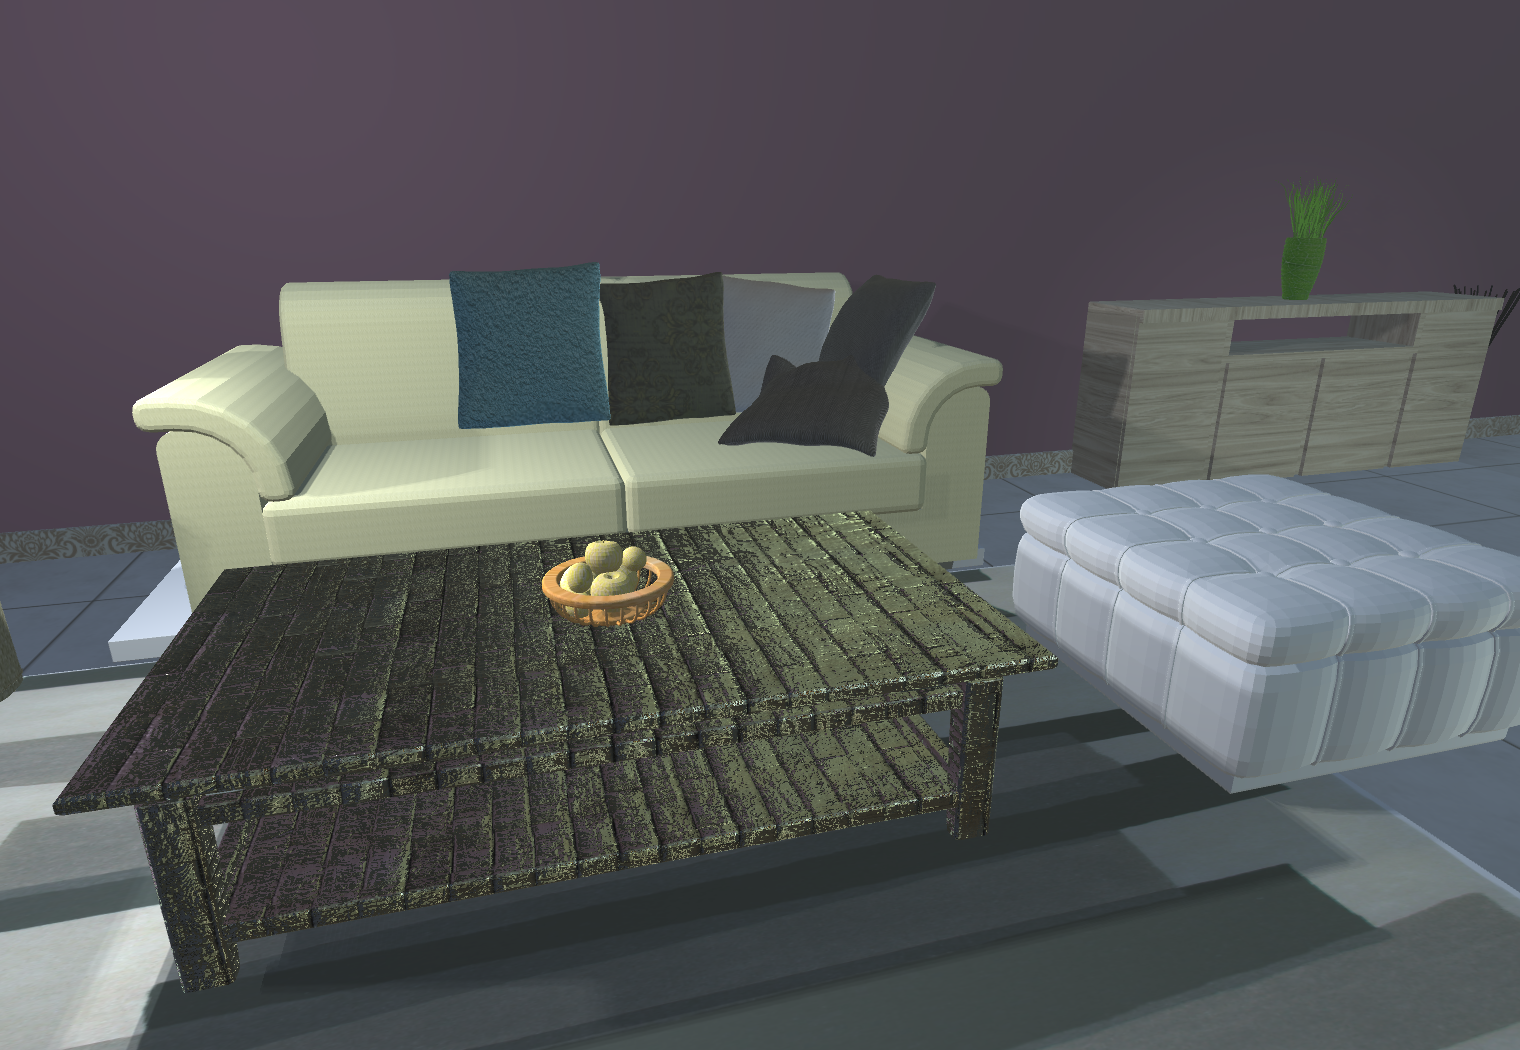
\includegraphics[width=.24\linewidth,valign=m]{/Users/apple/OVGU/Thesis/code/3dReconstruction/report/images/implementation/randomisation/lighting6}
    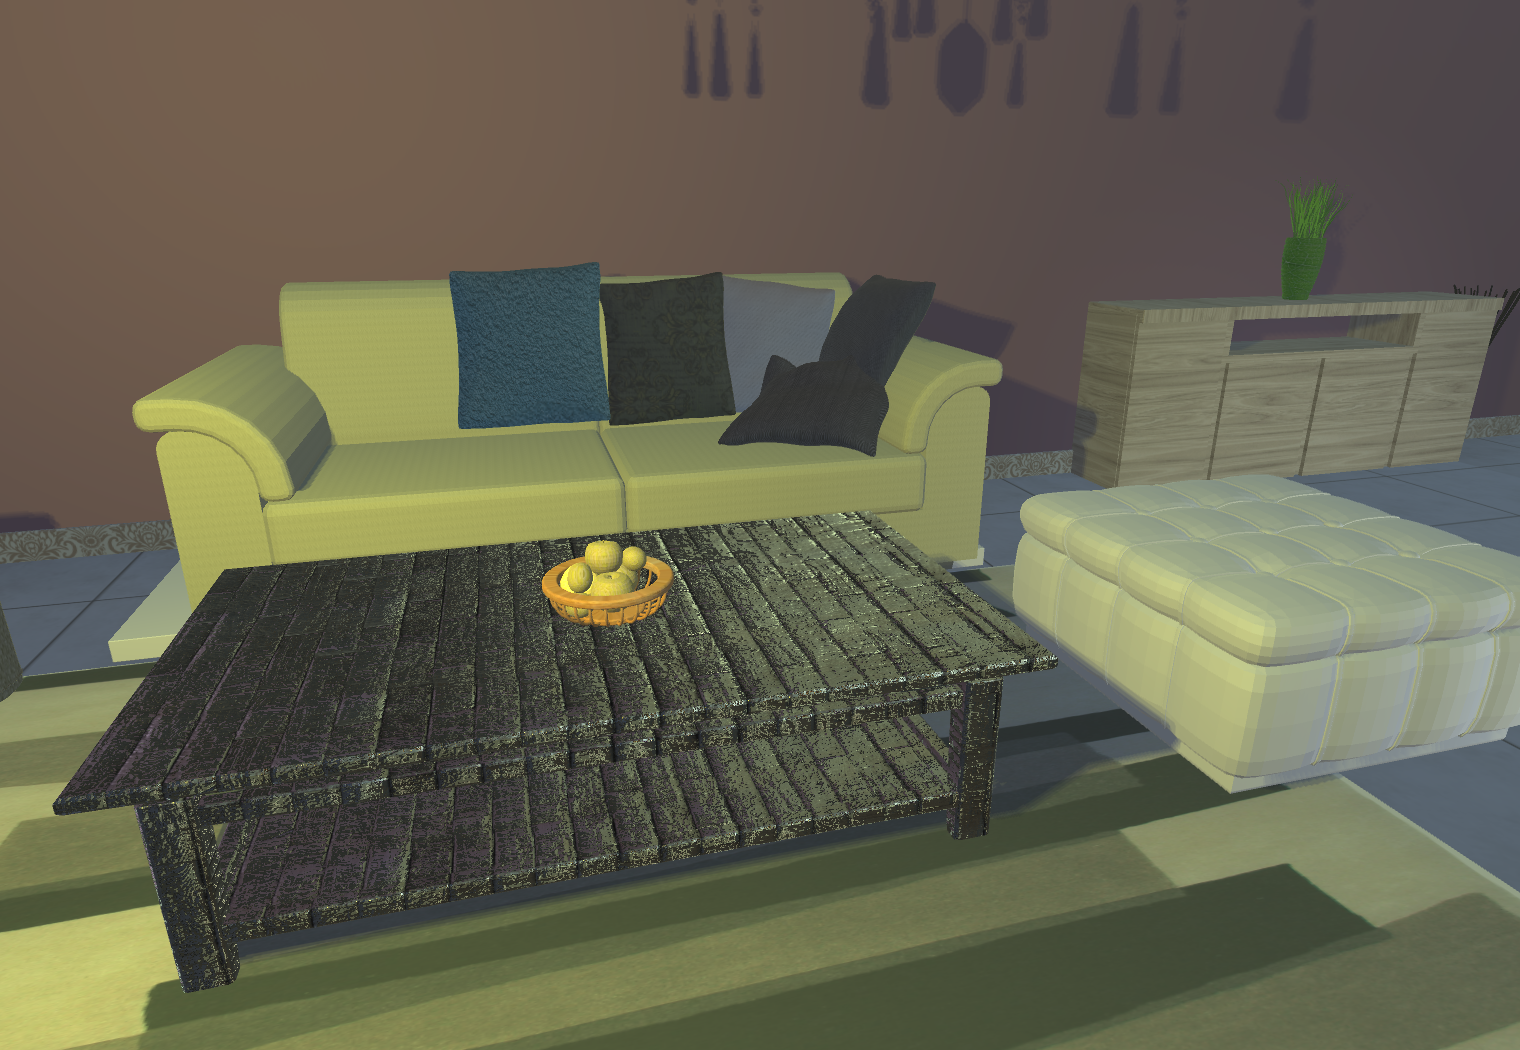
\includegraphics[width=.24\linewidth,valign=m]{/Users/apple/OVGU/Thesis/code/3dReconstruction/report/images/implementation/randomisation/lighting7}
    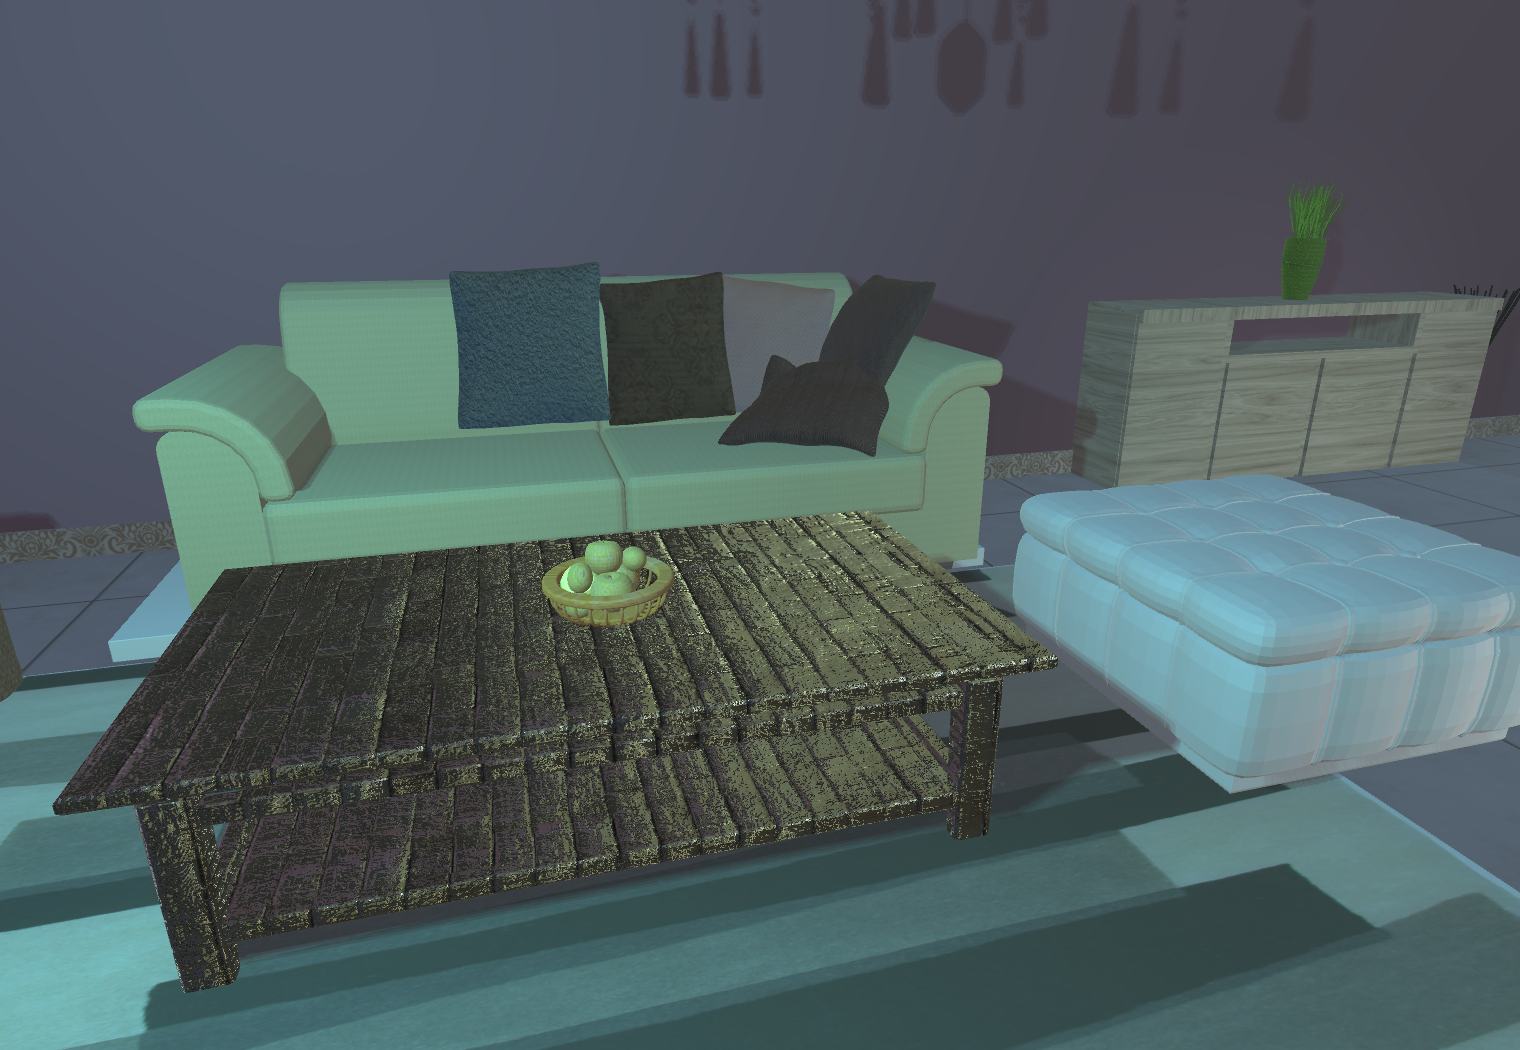
\includegraphics[width=.24\linewidth,valign=m]{/Users/apple/OVGU/Thesis/code/3dReconstruction/report/images/implementation/randomisation/lighting8}\\
    \caption[Samples for Lightings and Shadows.]{Sample images with different lighting and shadows conditions.First row is samples for light with different intensity and direction. Second row is differnt color for light.}
    \label{fig:Lighting and shadows}
\end{figure}

\section{3D Reconstruction Pipeline: Why Pix2Vox?}\label{sec:3D reconstruction pipeline}
We create a Deep Learning pipeline for processing the 3D reconstruction task.
The backbone of the pipeline is the base model and the dataset being used to train.
In this section, we discuss the model used as a base and the rationale behind its selection.

Pix2Vox has been used as a baseline by most of the research-oriented to 3D reconstruction.
This network is one of the few networks to be tested on the Pix3D dataset.
According to the survey conducted by~\cite{Han2021ImageBased3O}, the performance of Pix2Vox~\cite{Xie_2019}
is significantly higher compared to previous work(\cite{Tulsiani2017,tatarchenko2016multiview,Roth2018,Gwak2018,Johnston2017}), as shown in \autoref{fig:survey on 3d reconstruction}.
At the same time, this comparison was made on the 3D reconstruction of the ShapeNet dataset since Pix3D was not available when previous work was published.
From our survey, only CoReNet~\cite{popov2020corenet} had a slight gain in performance compared to Pix2Vox.
When trained on ShapeNet and tested with Pix3D, CoReNet gave a result of 29.7\% \gls{iou} while Pix2Vox gave a result of 28.8\% \gls{iou}  and Pix2Vox++ a result of 29.2\% \gls{iou}\@.
Since the difference in the performance was not significant, we decided to stick with the baseline model.
Another reason for selecting the Pix2Vox model is that the backbone of the architecture is pre-trained with ImageNet.
Hence, the embeddings generated from this encoder can help visualize the domain space of both Pix3D (real images)  and \gls{free}(synthetic images).
As mentioned above, for Pix2Vox++, the \gls{resnet} is the backbone encoder with 25\% lesser parameters and 5\% lesser inference time than \gls{vgg}\@.
In addition, the author even demonstrated that Pix2vox++ performs 1.5\% better than Pix2Vox.
The architecture of Pix2Vox++ is as shown in \autoref{fig:architectures}(b).
Furthermore, the focus of this thesis is not to check which is the best model to reconstruct the furniture but to check if game engines can produce photorealistic images usable for 3D reconstruction.
Hence the selection of the model was not of utmost importance.
However, since the two architectures are relatable, it would be interesting to compare the results for the 3D Reconstruction task.

%\begin{figure}
%    \centering
%    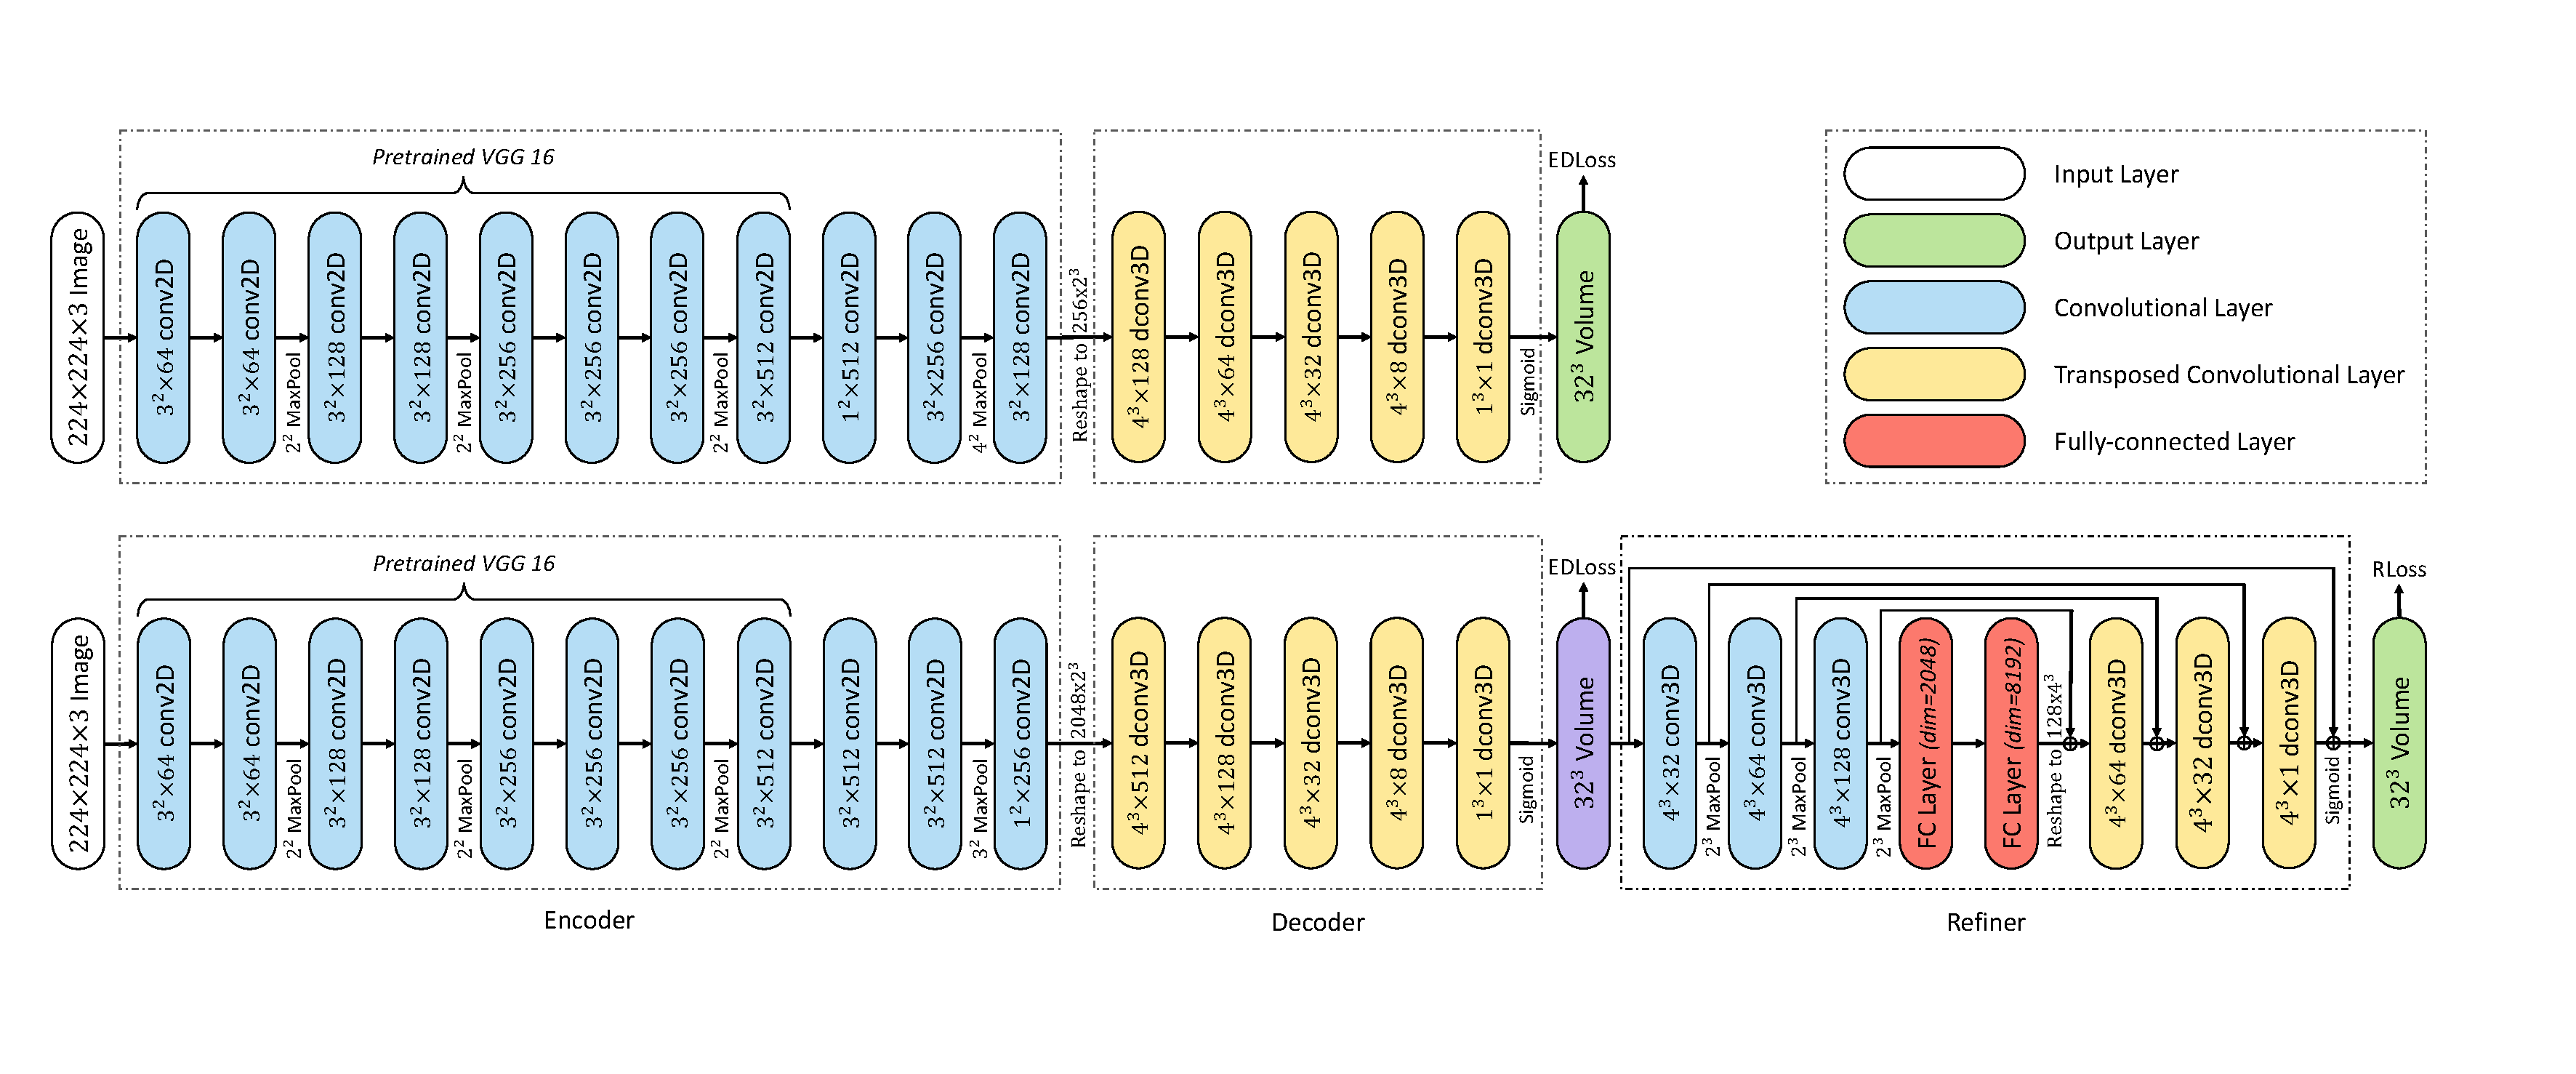
\includegraphics[width=\textwidth]{/Users/apple/OVGU/Thesis/code/3dReconstruction/report/images/concept/pix2vox}
%    \caption{Network architecture for pix2vox~\cite{Xie_2019}}
%    \label{fig:pix2vox architecture}
%\end{figure}
%
%\begin{figure}
%    \centering
%    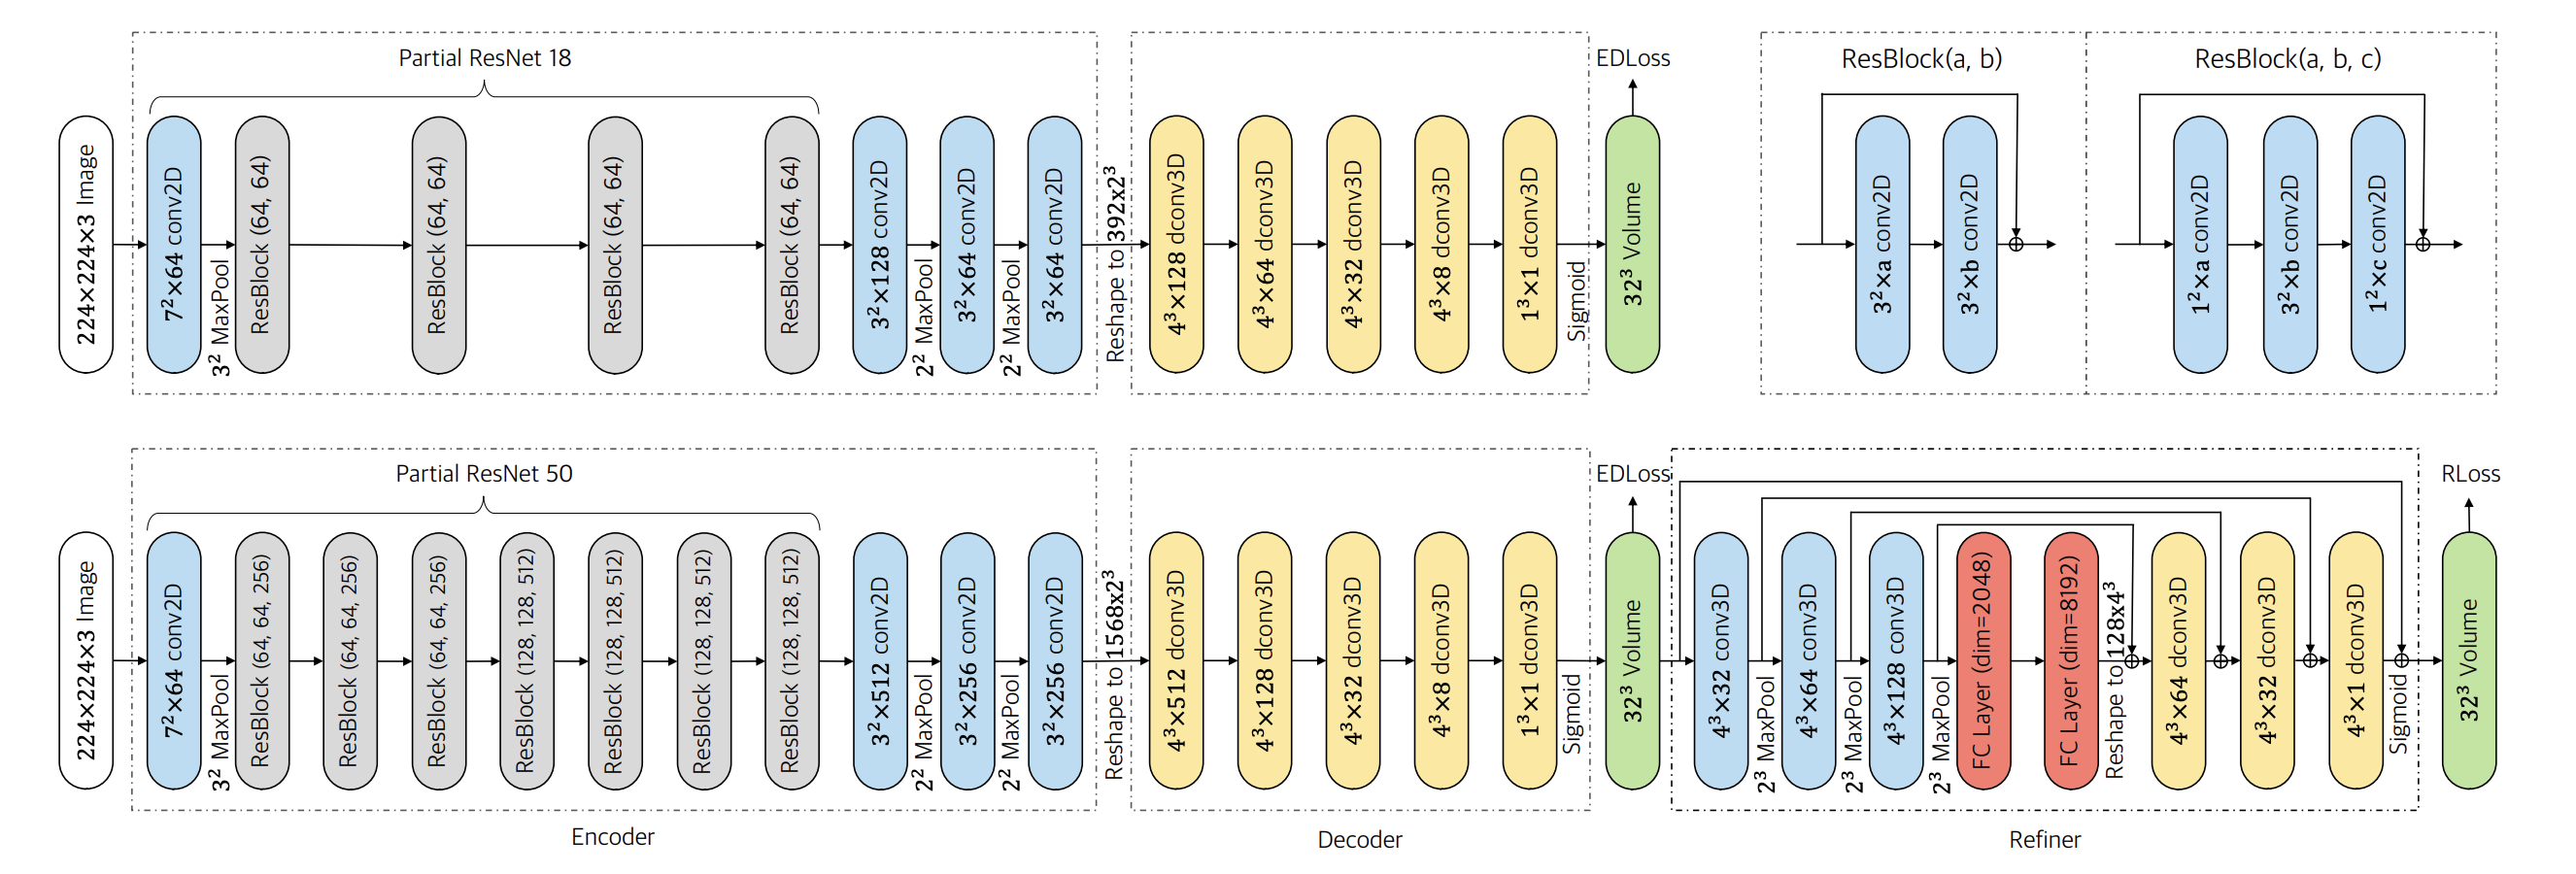
\includegraphics[width=\textwidth]{/Users/apple/OVGU/Thesis/code/3dReconstruction/report/images/concept/pix2voxpp}
%    \caption{Network architecture for pix2vox++~\cite{Xie_2020}}
%    \label{fig:pix2voxpp architecture}
%\end{figure}

\begin{figure}[ht]
    \centering
    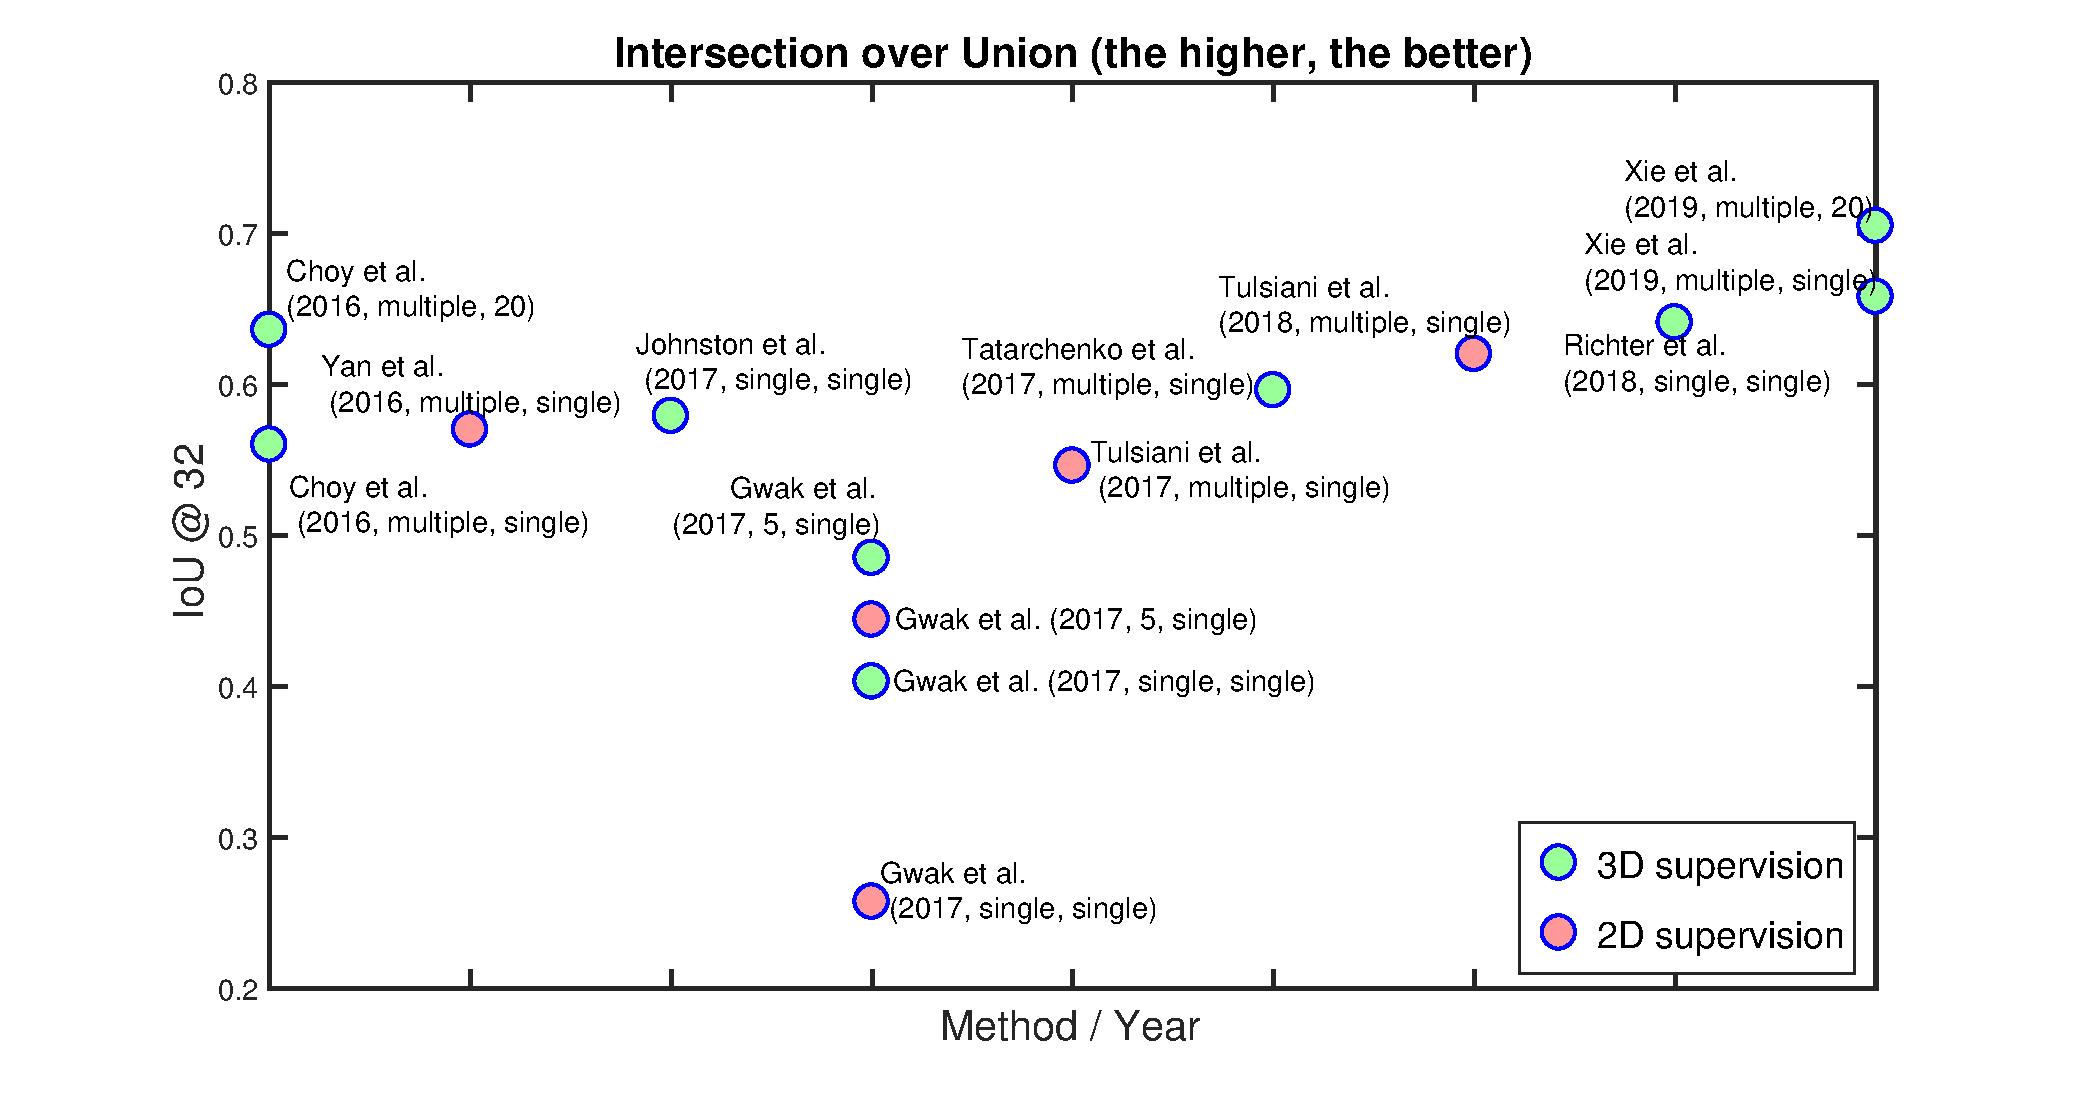
\includegraphics[width=\textwidth]{/Users/apple/OVGU/Thesis/code/3dReconstruction/report/images/concept/survey}
    \caption[Survey Results for 3D-Reconstruction.]{A survey conducted by~\cite{Han2021ImageBased3O}, demonstrates that Pix2Vox is considerably a good 3D reconstruction model.
    The values are from 3D reconstruction of ShapeNet~\cite{shapenet2015} since Pix3D was not published by then.}
    \label{fig:survey on 3d reconstruction}
\end{figure}


\section{Datasets}\label{sec:datasets}
In this section, we describe the datasets used for the evaluations.
Datasets intend to have variations in domain randomization to check their performance on the 3D reconstruction tasks.

\subsection{Pix3D}\label{subsec:pix3d}
As mentioned in \autoref{subsec:why-pix3d?}, we use a real dataset from~\cite{Sun2018}, a collection of indoor scenes.
The two classes ’misc’ and ’tools’ are eliminated to focus only on furniture.
The total images after the reduction are 9954 with 354 unique models.
The dataset is divided into 70:30, giving us 6814 images from training and 3140 images for validation/test.
We do not have a test set only for this dataset since it is already limited, and the validation set is used as a test set while testing with synthetic data.
Samples are as shown in \autoref{fig:samples for synthetic and real comparison}.

\subsection{\gls{s2rv1}}\label{subsec:gls{free}-version-1}
Version 1 of \gls{free} was created by keeping the models in the center of a default 3D room.
The camera distance was randomized between 1 and 2.5 meters from the model.
The camera viewpoints and textures were randomized.
A total of 70000 images were synthetically generated using the \gls{free} `Single Room pipeline' with 10000 images per category.
Samples are as shown in \autoref{fig:samples for synthetic and real comparison}.

\subsection{\gls{s2rv2}}\label{subsec:gls{free}-version-2}
Version 1 of \gls{free} was created by keeping the models in the center of a default 3D room.
The distance of the camera was randomly chosen between 1 and 2.5 meters from the model.
The camera viewpoints and textures were randomized.
A total of 21000 images were synthetically generated using the \gls{free} `Multi-Object pipeline' with 3000 images per category.
Samples are as shown in \autoref{fig:samples for synthetic and real comparison}.

\begin{figure}[ht]
    \centering
    \begin{tabular}{llll}
        Pix3D & 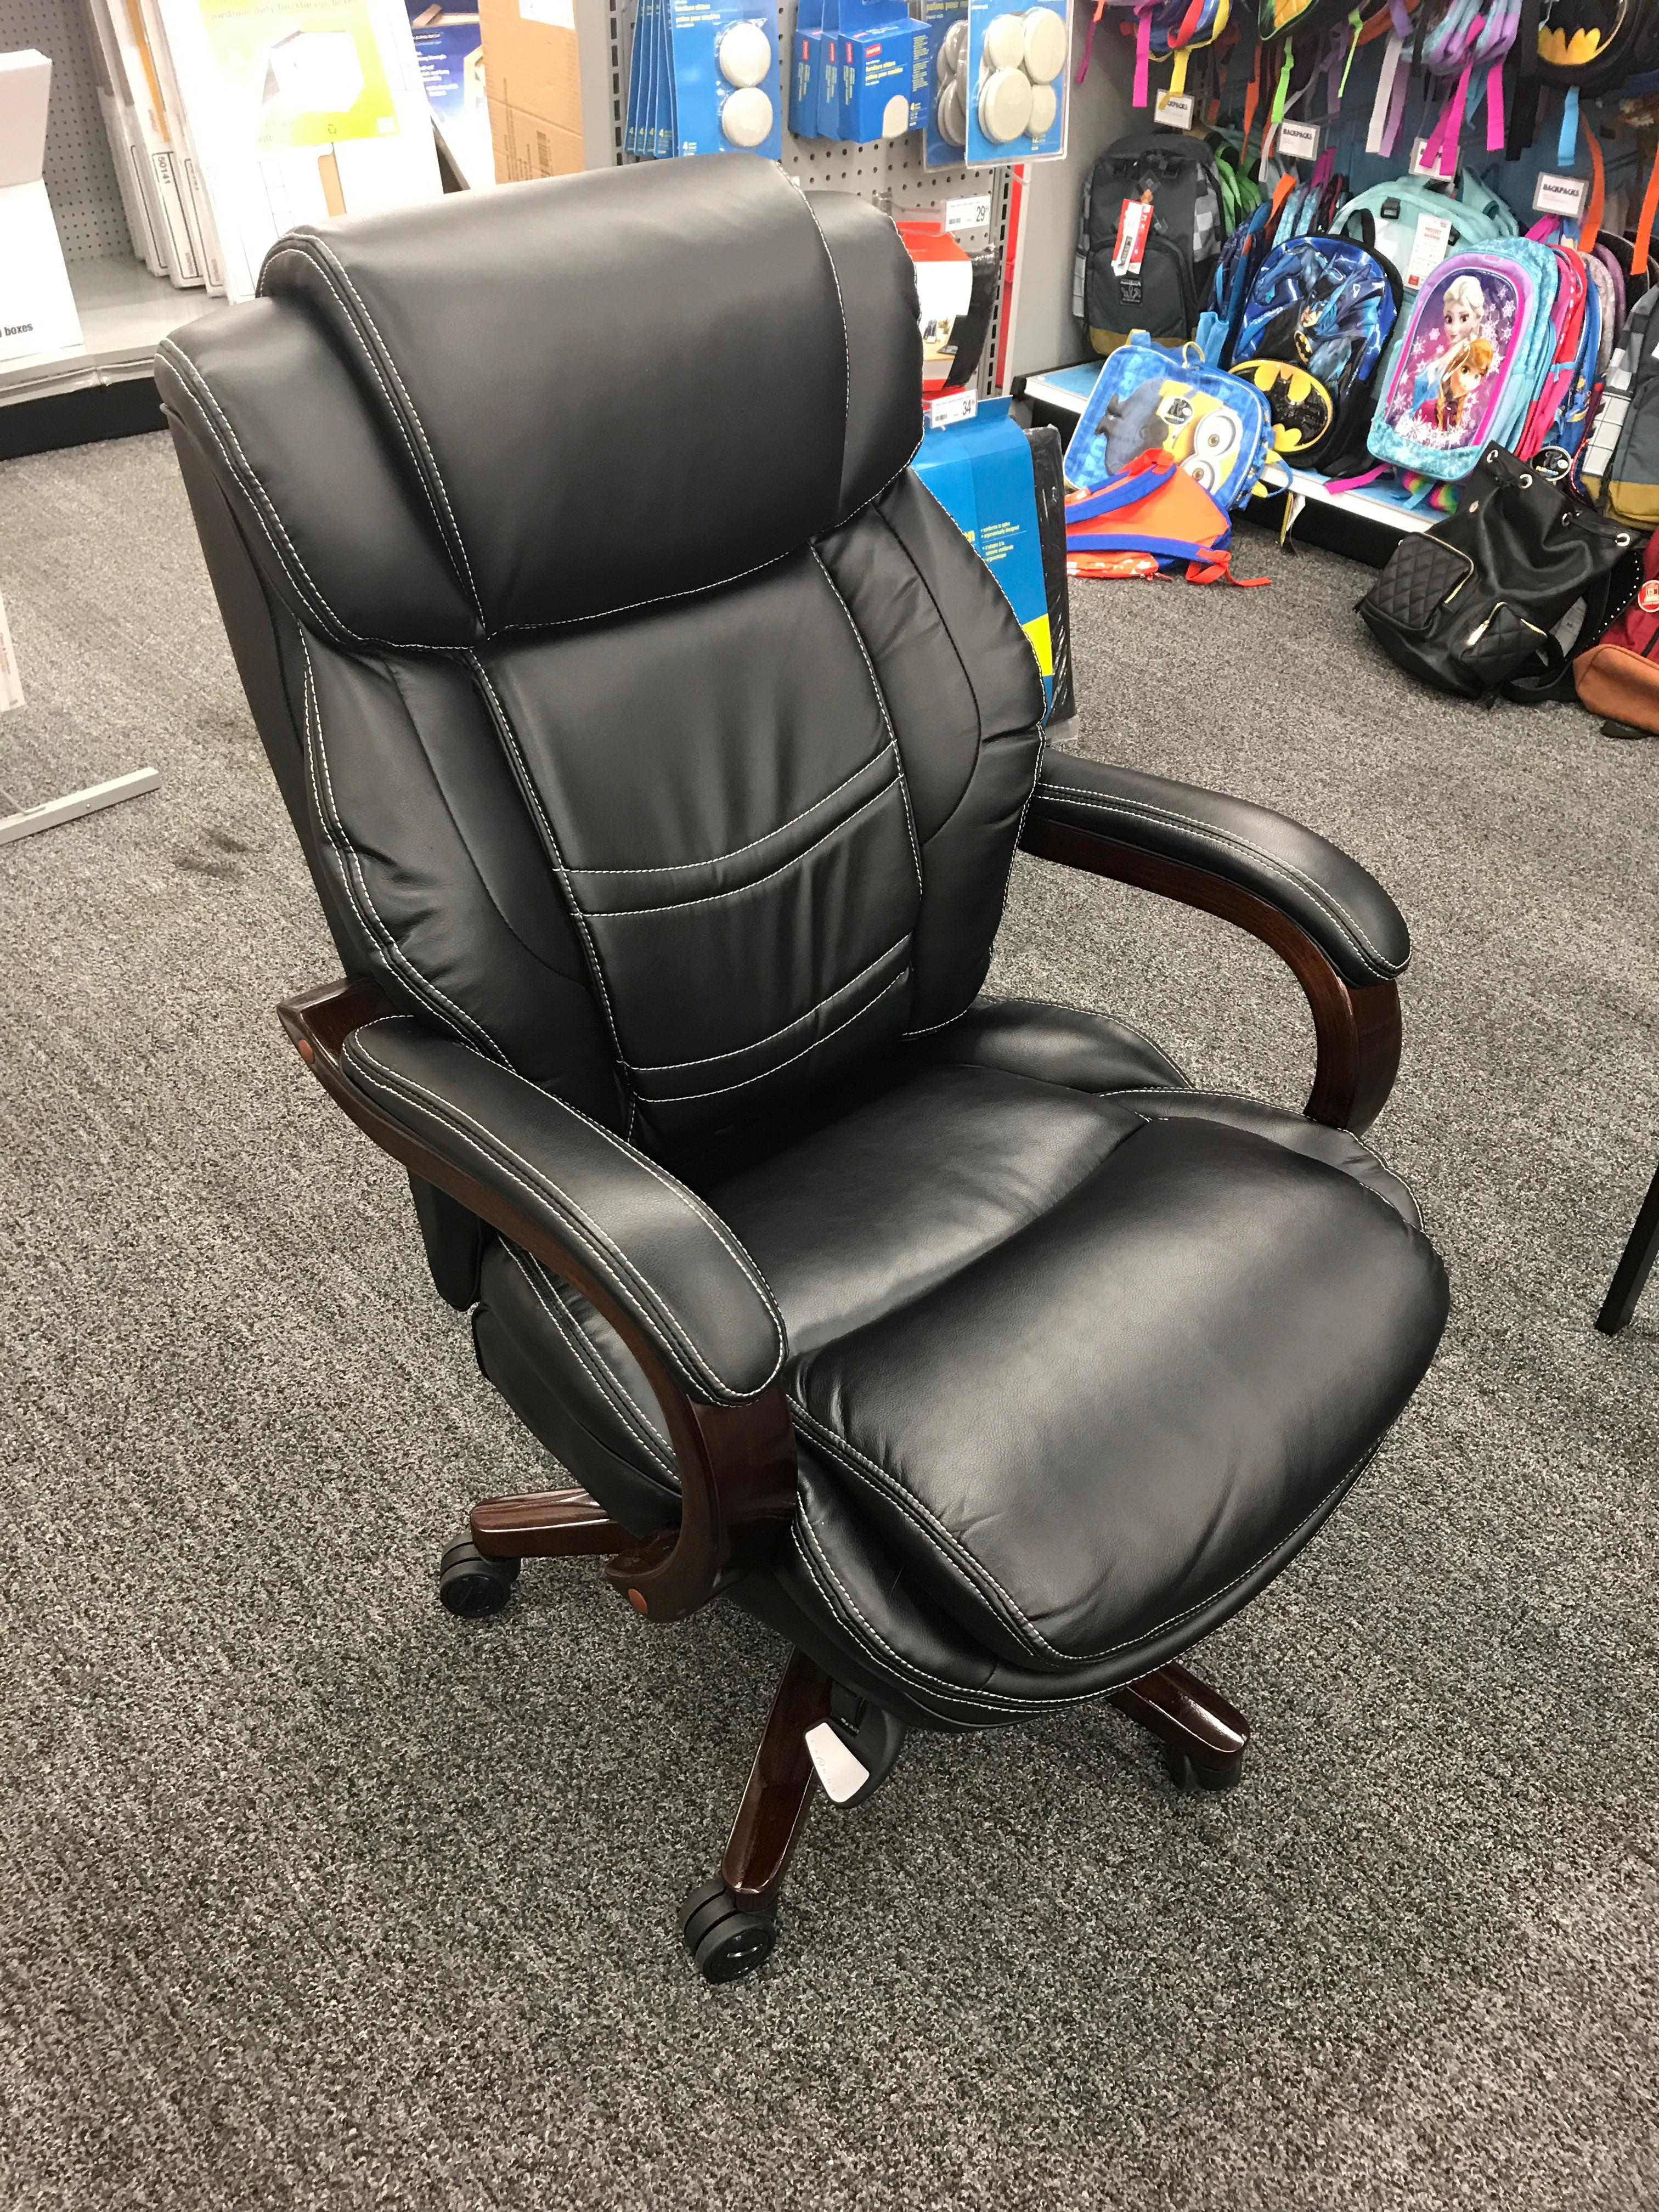
\includegraphics[width=.2\textwidth, height =.19\textwidth]{/Users/apple/OVGU/Thesis/code/3dReconstruction/report/images/evaluation/datasets/pix3d_1} &
        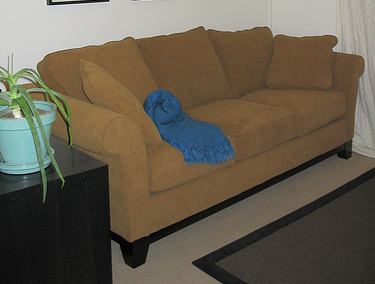
\includegraphics[width=.2\textwidth, height =.19\textwidth]{/Users/apple/OVGU/Thesis/code/3dReconstruction/report/images/evaluation/datasets/pix3d_2} &
        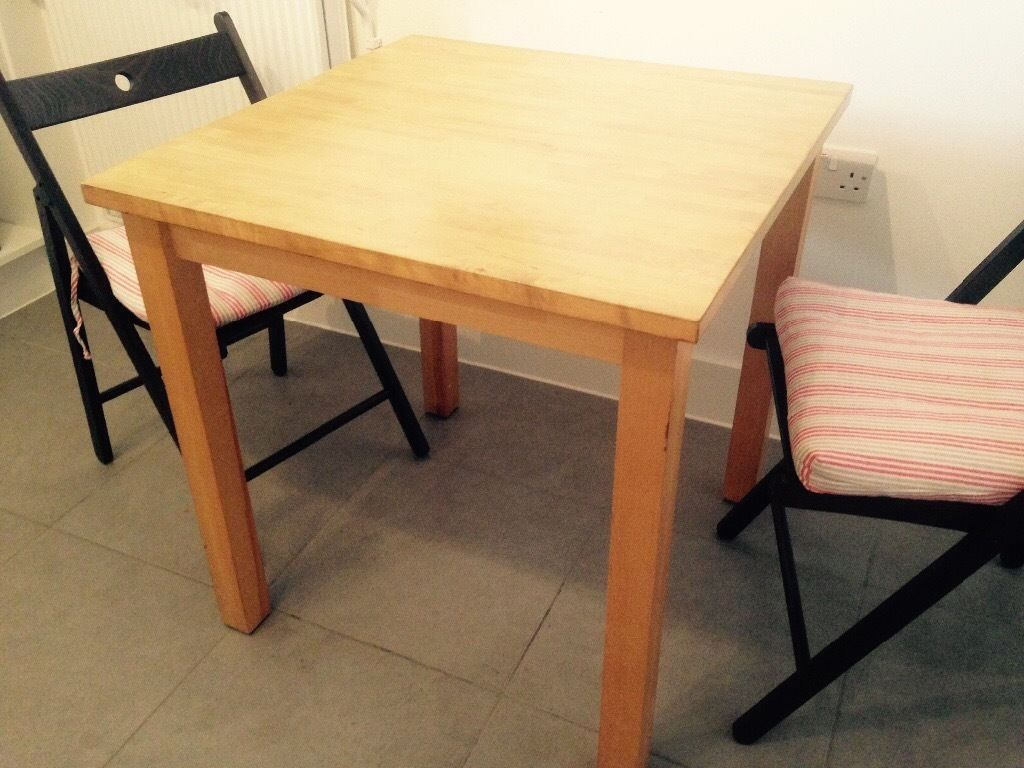
\includegraphics[width=.2\textwidth, height =.19\textwidth]{/Users/apple/OVGU/Thesis/code/3dReconstruction/report/images/evaluation/datasets/pix3d_3}\\

        \gls{s2rv1} & 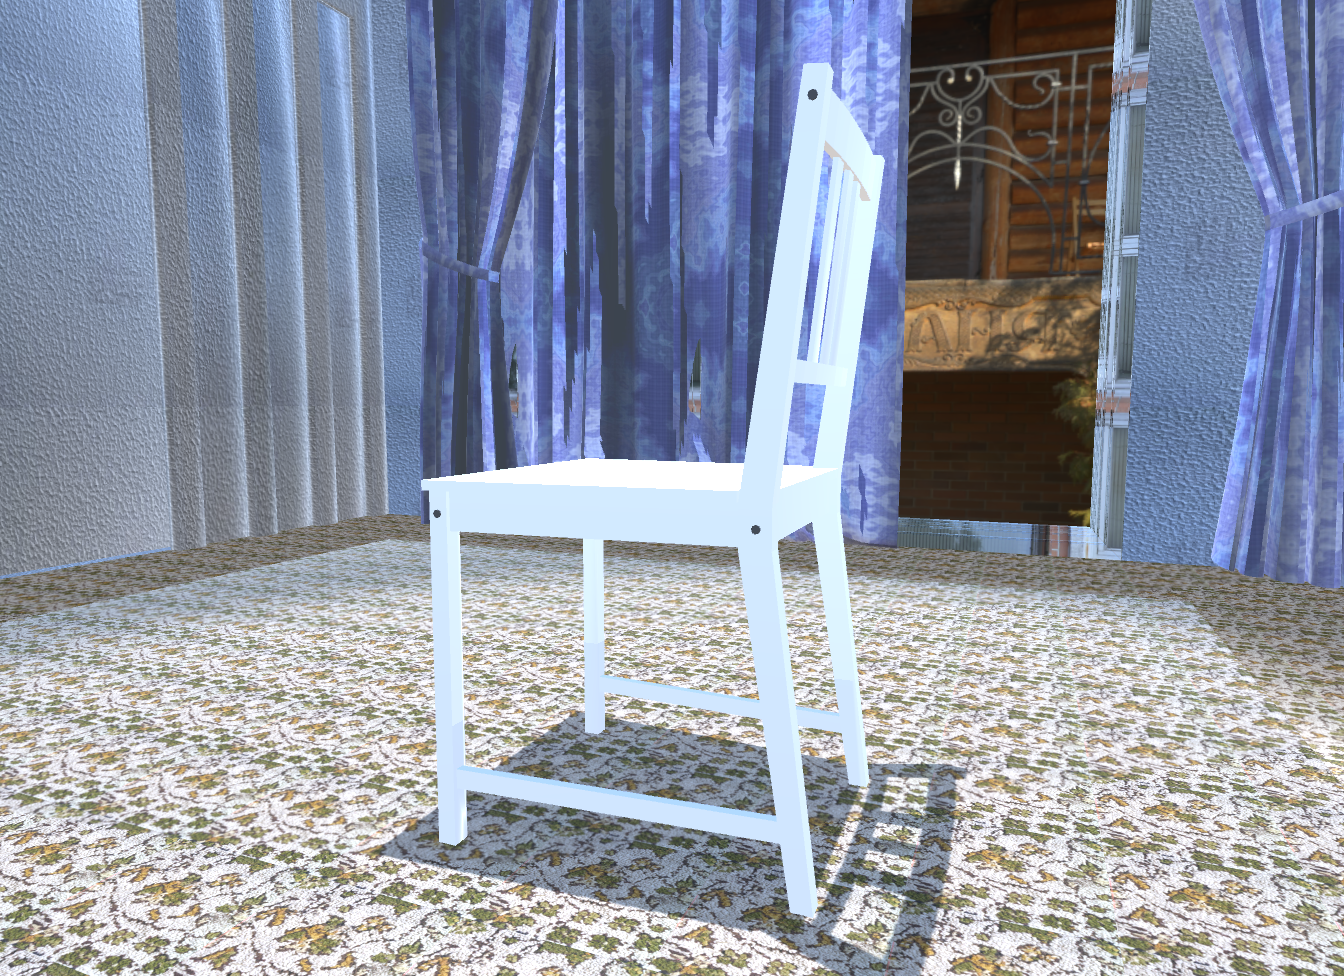
\includegraphics[width=.2\textwidth, height =.19\textwidth]{/Users/apple/OVGU/Thesis/code/3dReconstruction/report/images/evaluation/datasets/s2r_v1_1} &
        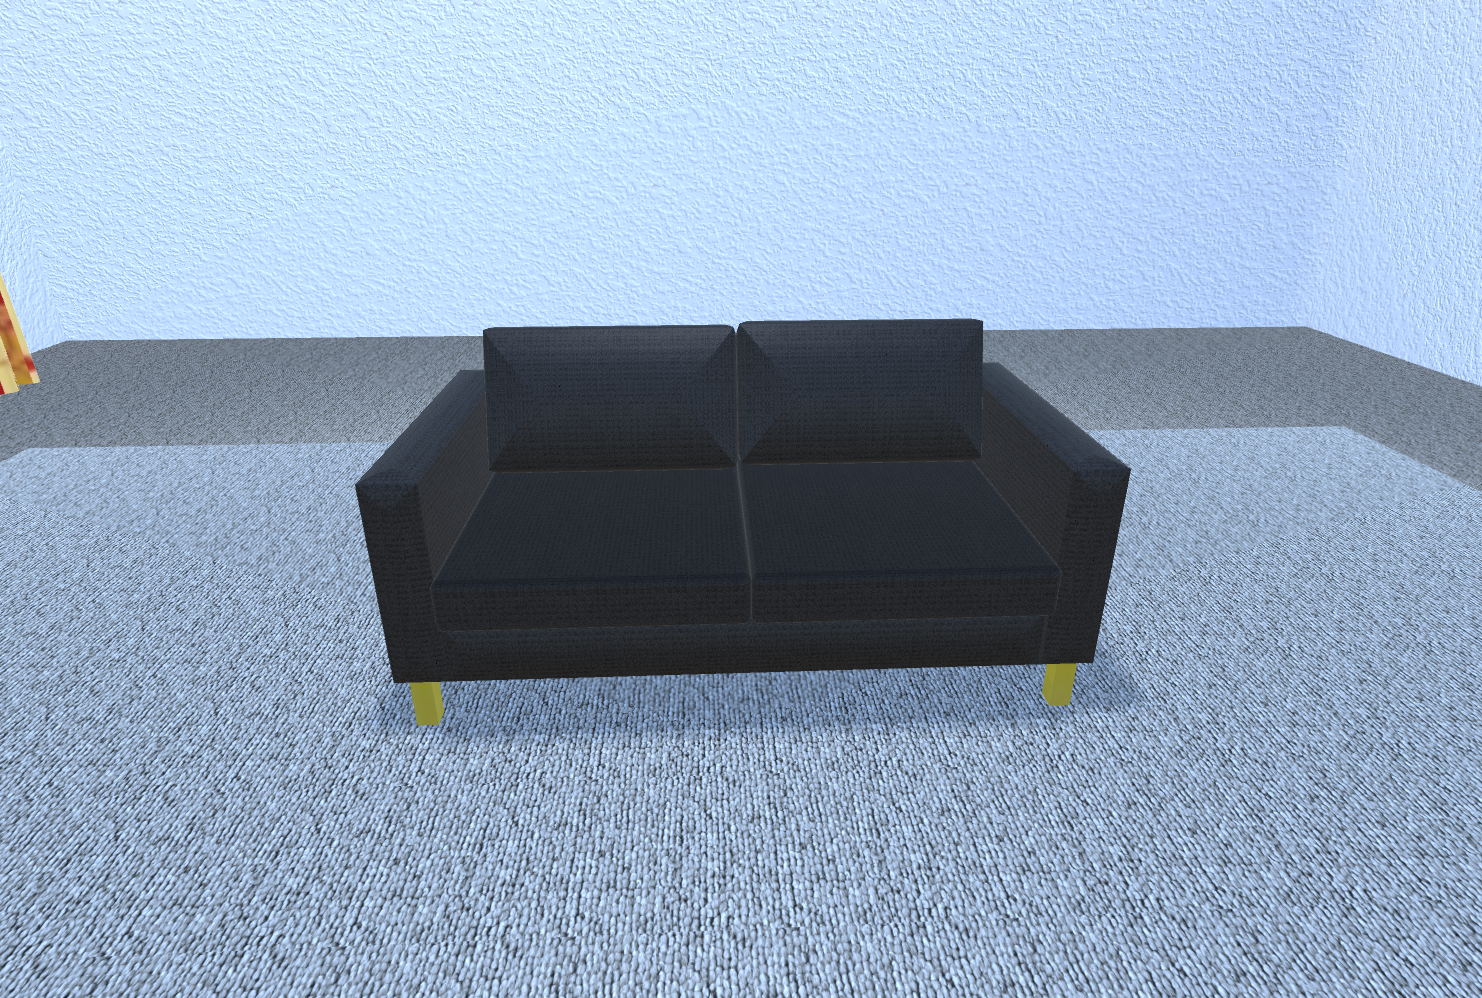
\includegraphics[width=.2\textwidth, height=.19\textwidth]{/Users/apple/OVGU/Thesis/code/3dReconstruction/report/images/evaluation/datasets/s2r_v1_2} &
        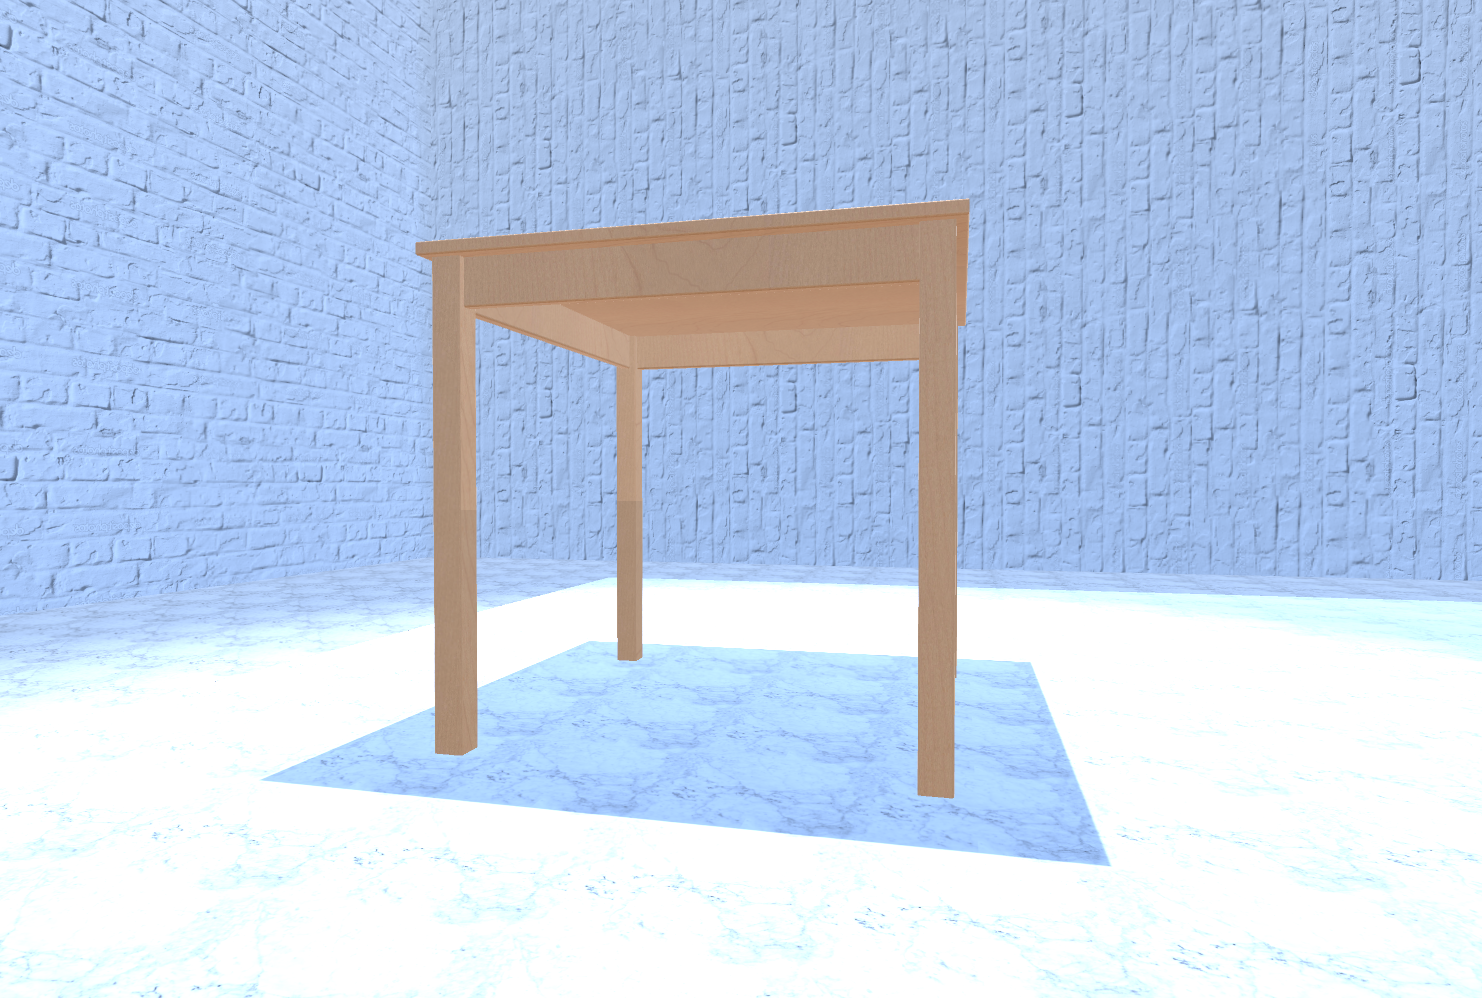
\includegraphics[width=.2\textwidth, height=.19\textwidth]{/Users/apple/OVGU/Thesis/code/3dReconstruction/report/images/evaluation/datasets/s2r_v1_3}\\

        \gls{s2rv2} & 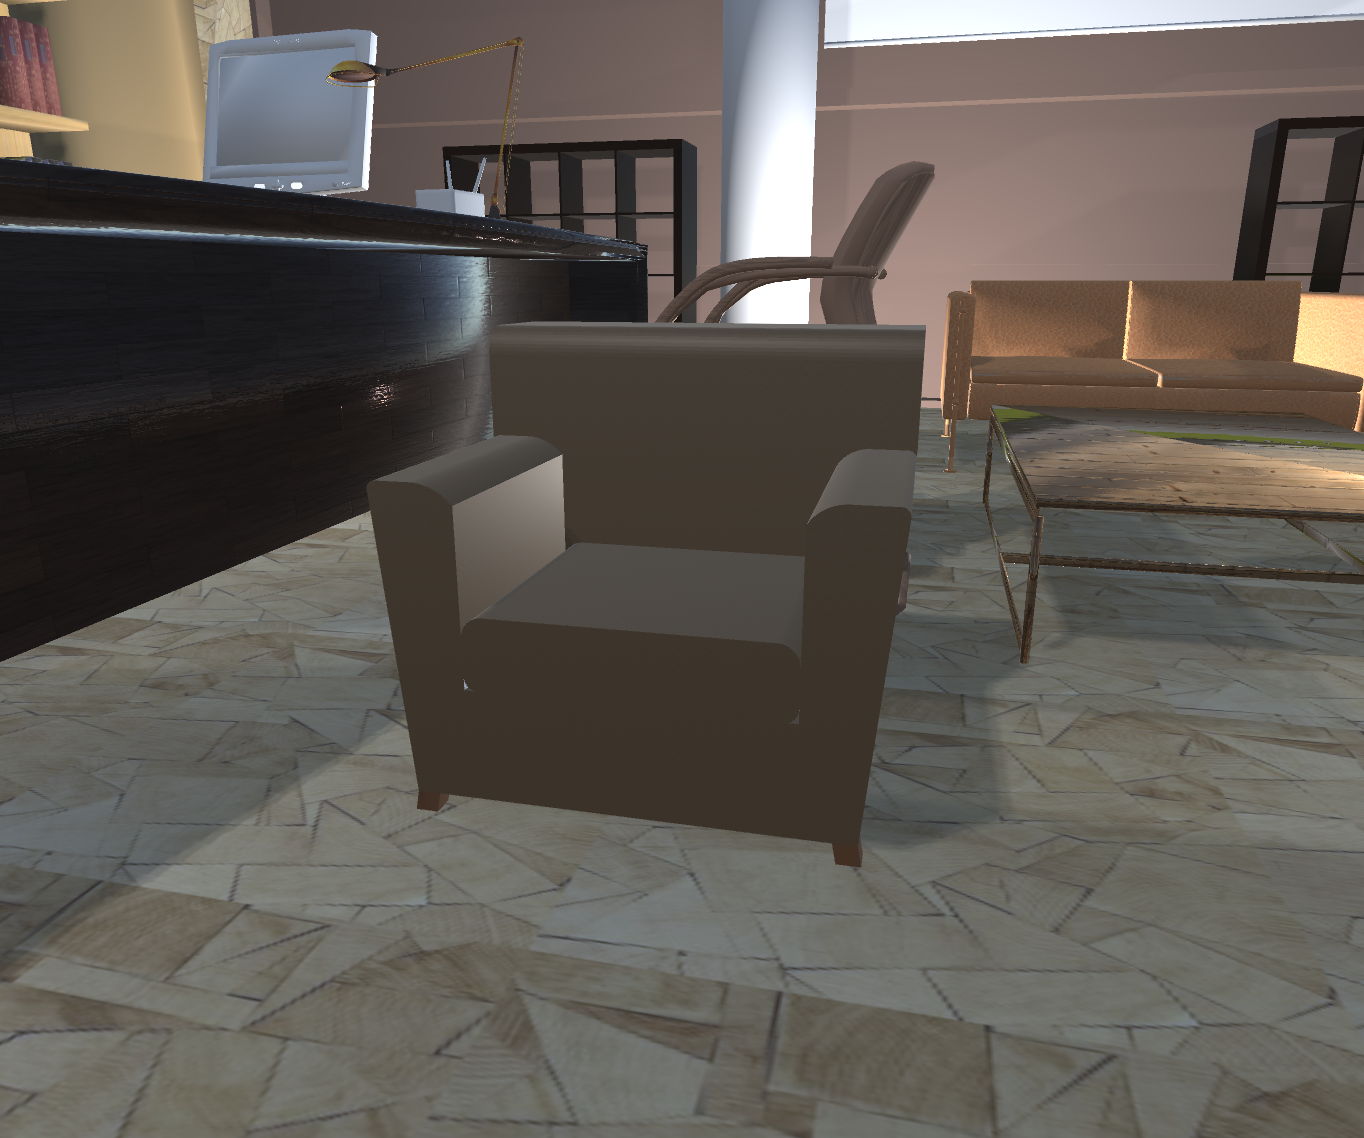
\includegraphics[width=.19\textwidth, height =.2\textwidth]{/Users/apple/OVGU/Thesis/code/3dReconstruction/report/images/evaluation/datasets/s2r_v3_1} &
        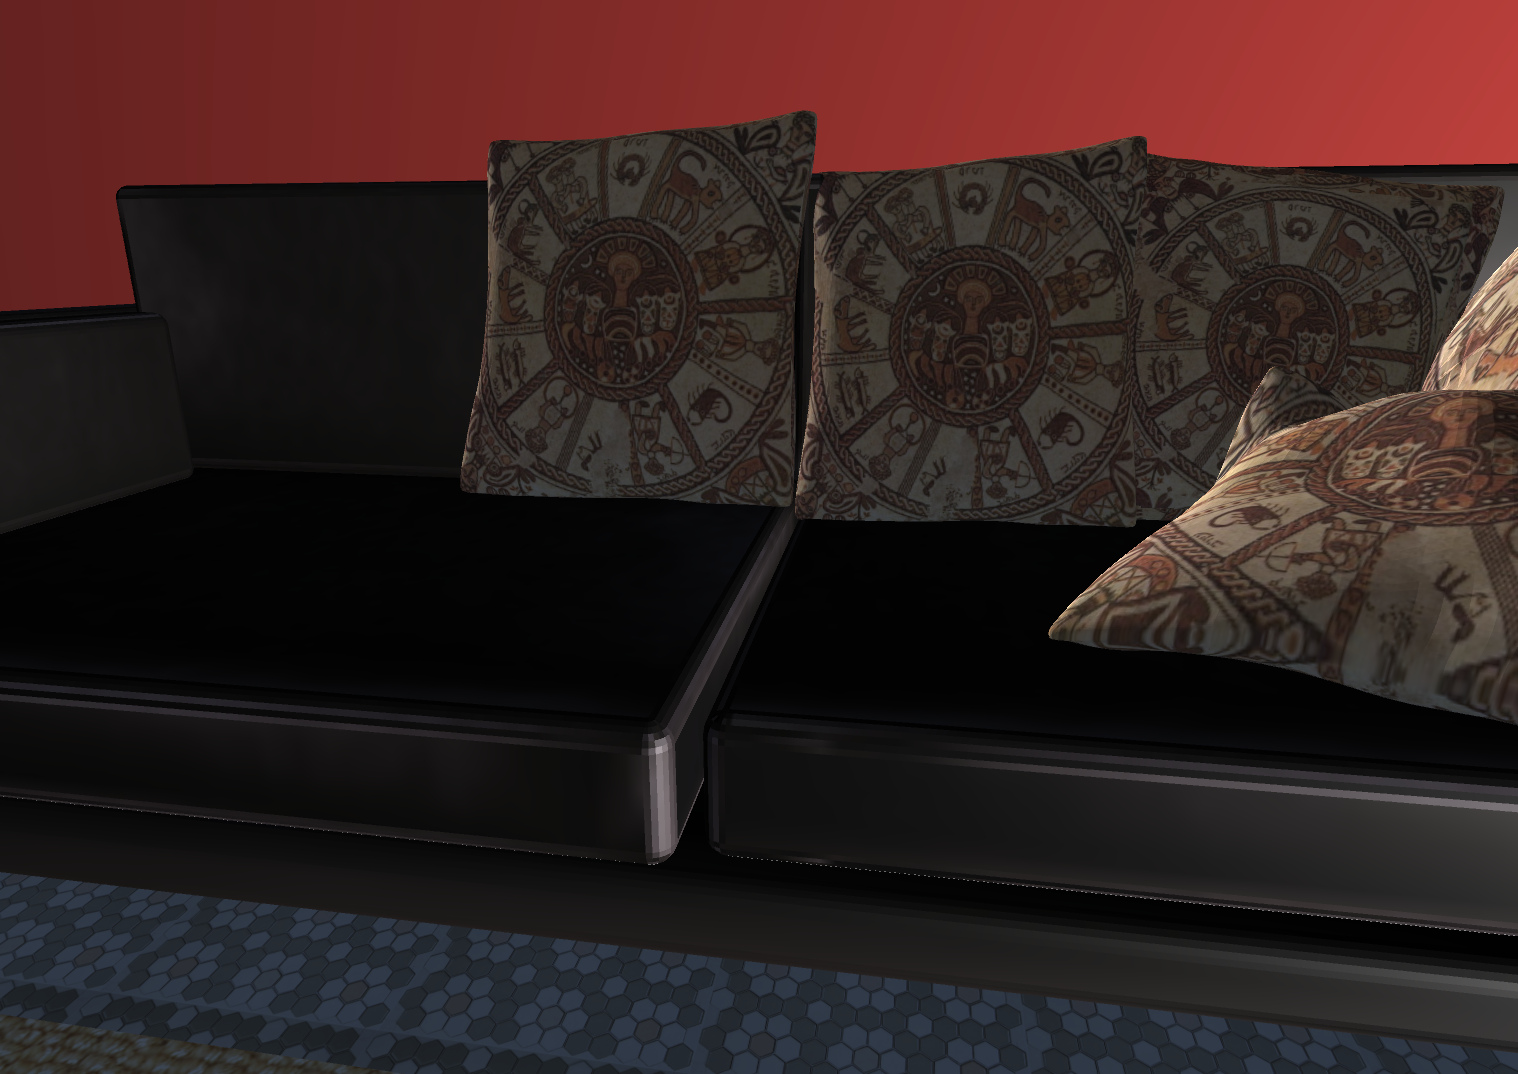
\includegraphics[width=.2\textwidth, height=.19\textwidth]{/Users/apple/OVGU/Thesis/code/3dReconstruction/report/images/evaluation/datasets/s2r_v3_2} &
        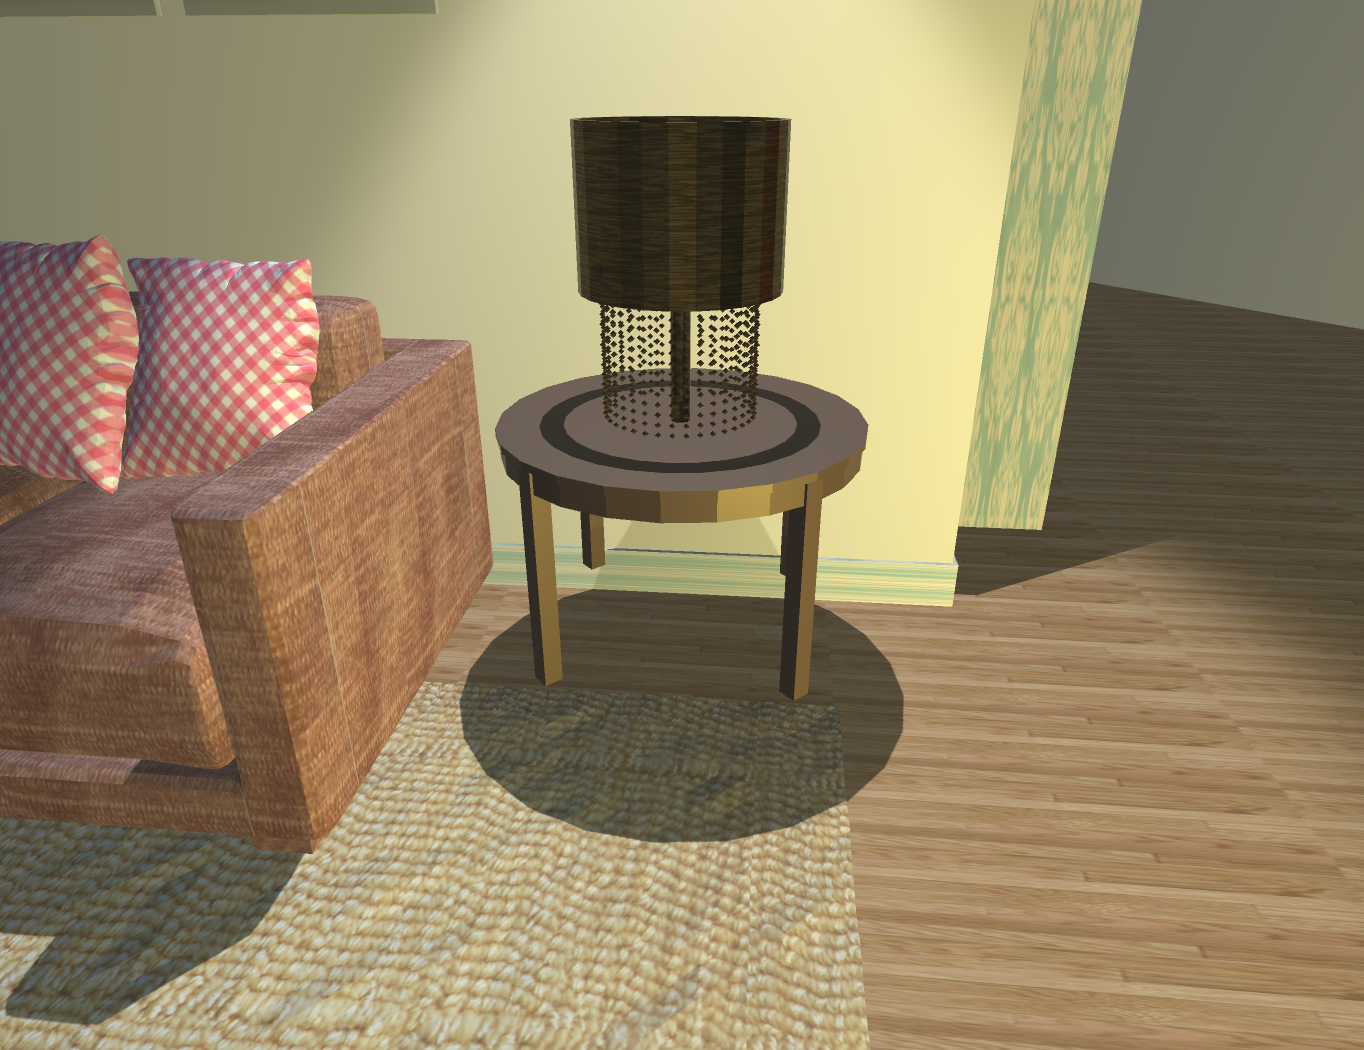
\includegraphics[width=.2\textwidth, height=.19\textwidth]{/Users/apple/OVGU/Thesis/code/3dReconstruction/report/images/evaluation/datasets/s2r_v3_3}\\

    \end{tabular}
    \caption[Samples for Real and Synthetic Datasets]{Samples of images from real and synthetic datasets.}
    \label{fig:samples for synthetic and real comparison}
\end{figure}

\subsection{\gls{free} Ablation}\label{subsec:s2r:3dfree-ablation}
Pix3D is composed of 3839 chairs which is the maximum among all categories.
To study the effects of domain randomization, we create multiple chair datasets by omitting randomizing factors one at a time and study the model behavior.
We divide the datasets into five categories with different randomization parameters.
The sample images with different randomization are as shown in \autoref{fig:domain_randomisation_for_ablation_study}.

\begin{figure}[!ht]
    \begin{tabular}{llll}
        Textureless & 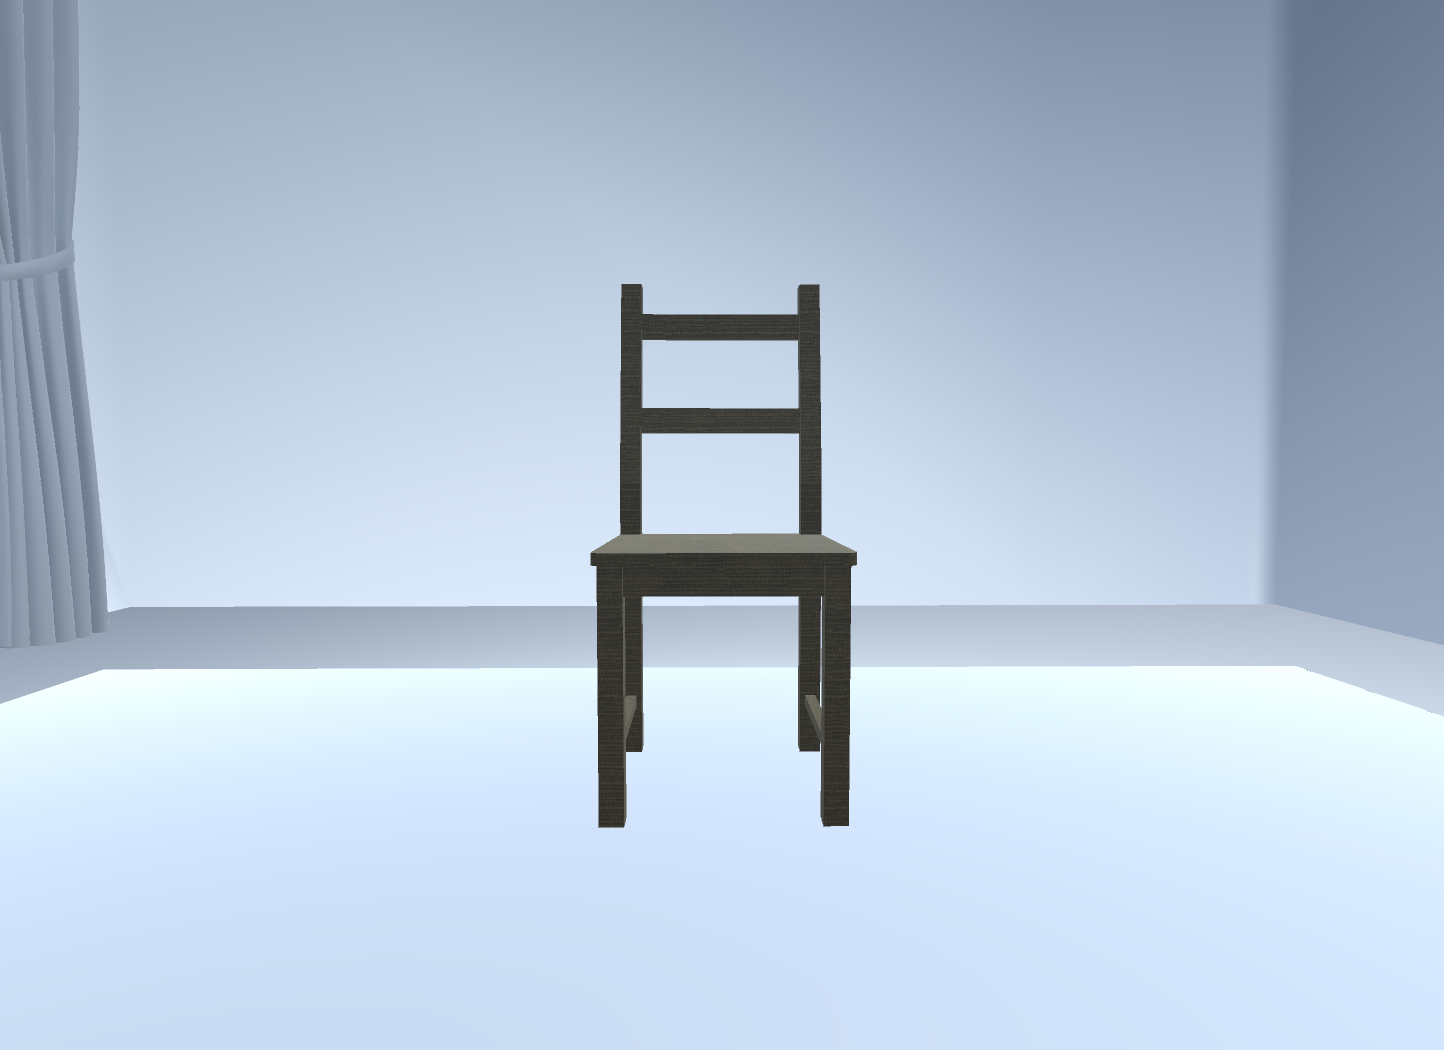
\includegraphics[width=.2\linewidth]{/Users/apple/OVGU/Thesis/code/3dReconstruction/report/images/evaluation/datasets/s2r_textureless_1} &
        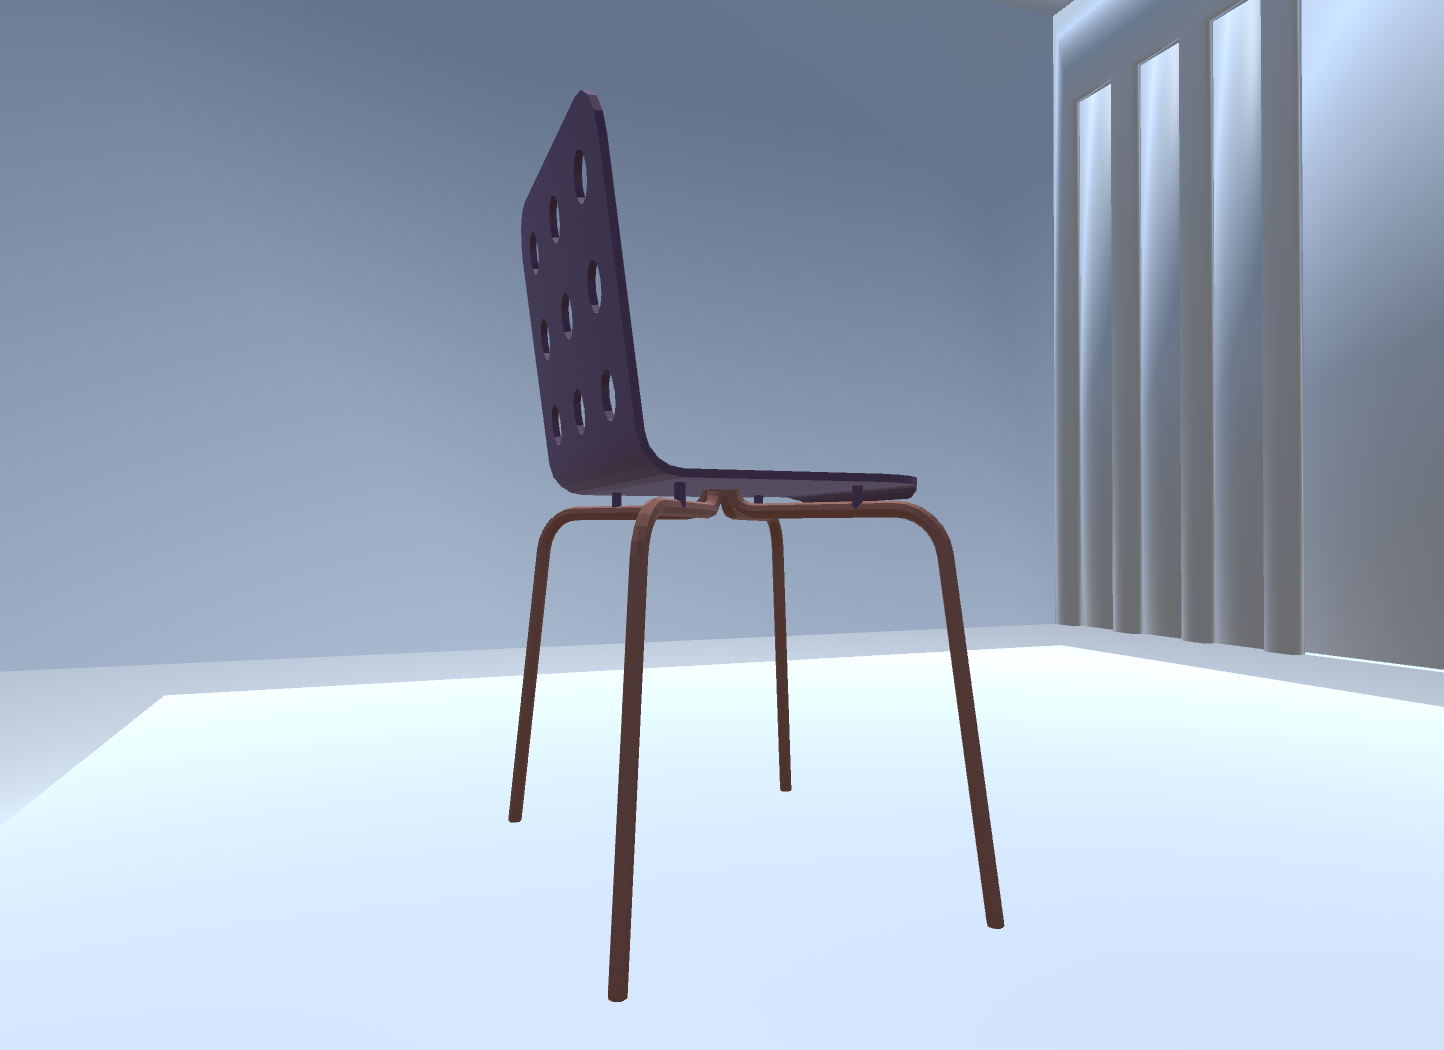
\includegraphics[width=.2\linewidth]{/Users/apple/OVGU/Thesis/code/3dReconstruction/report/images/evaluation/datasets/s2r_textureless_2} &
        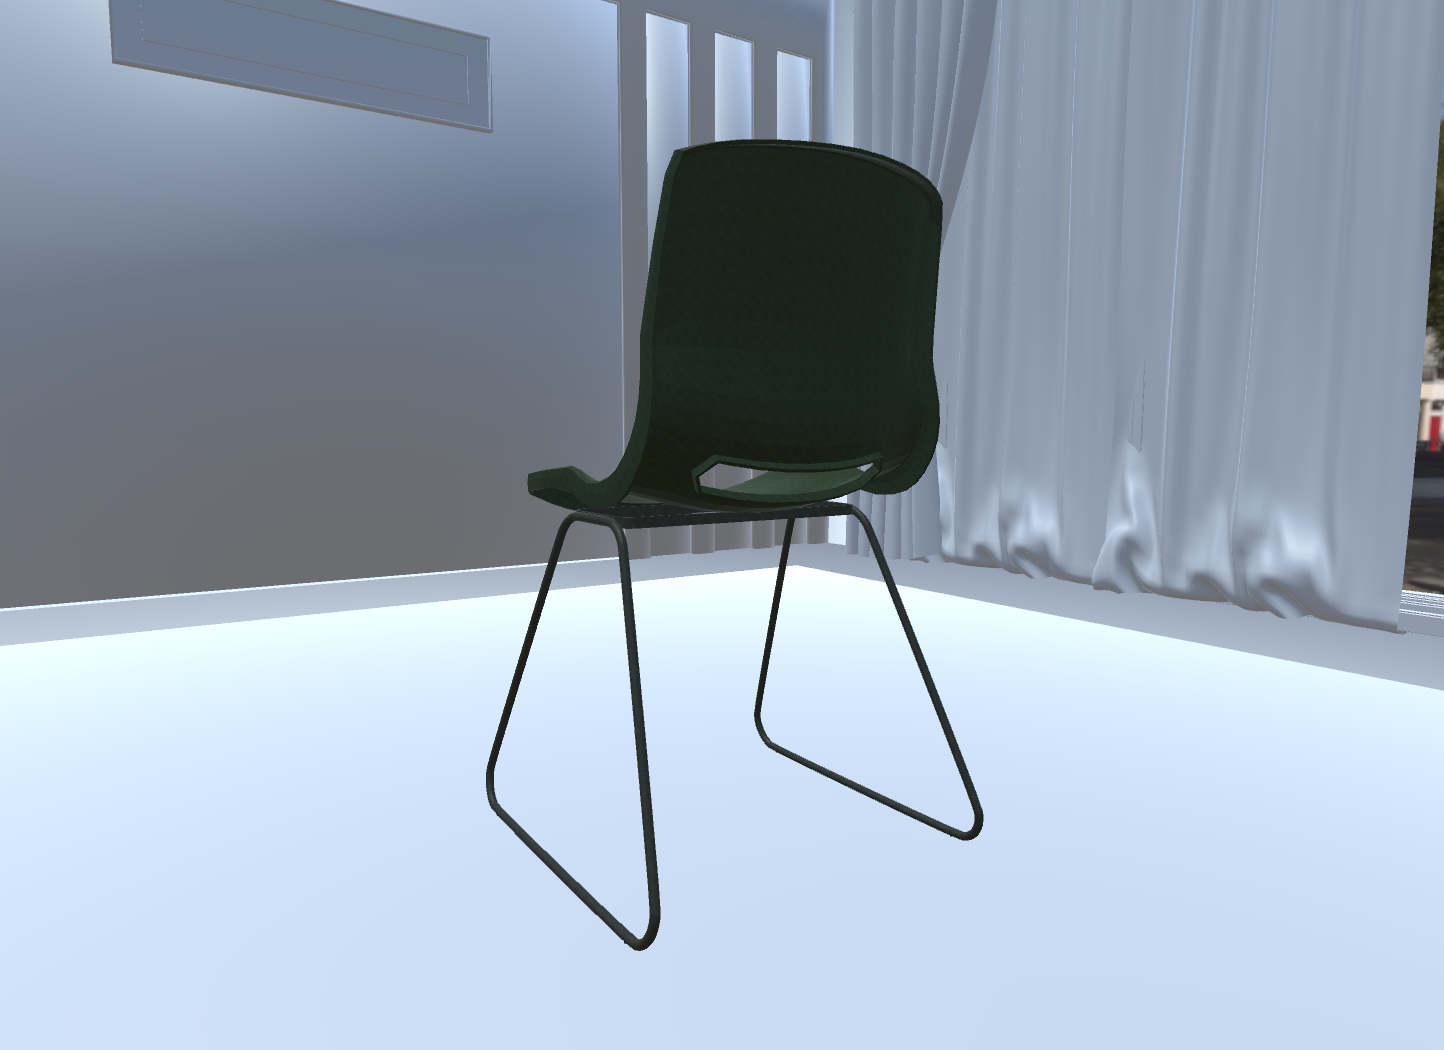
\includegraphics[width=.2\linewidth]{/Users/apple/OVGU/Thesis/code/3dReconstruction/report/images/evaluation/datasets/s2r_textureless_3}\\

        Textureless with light & 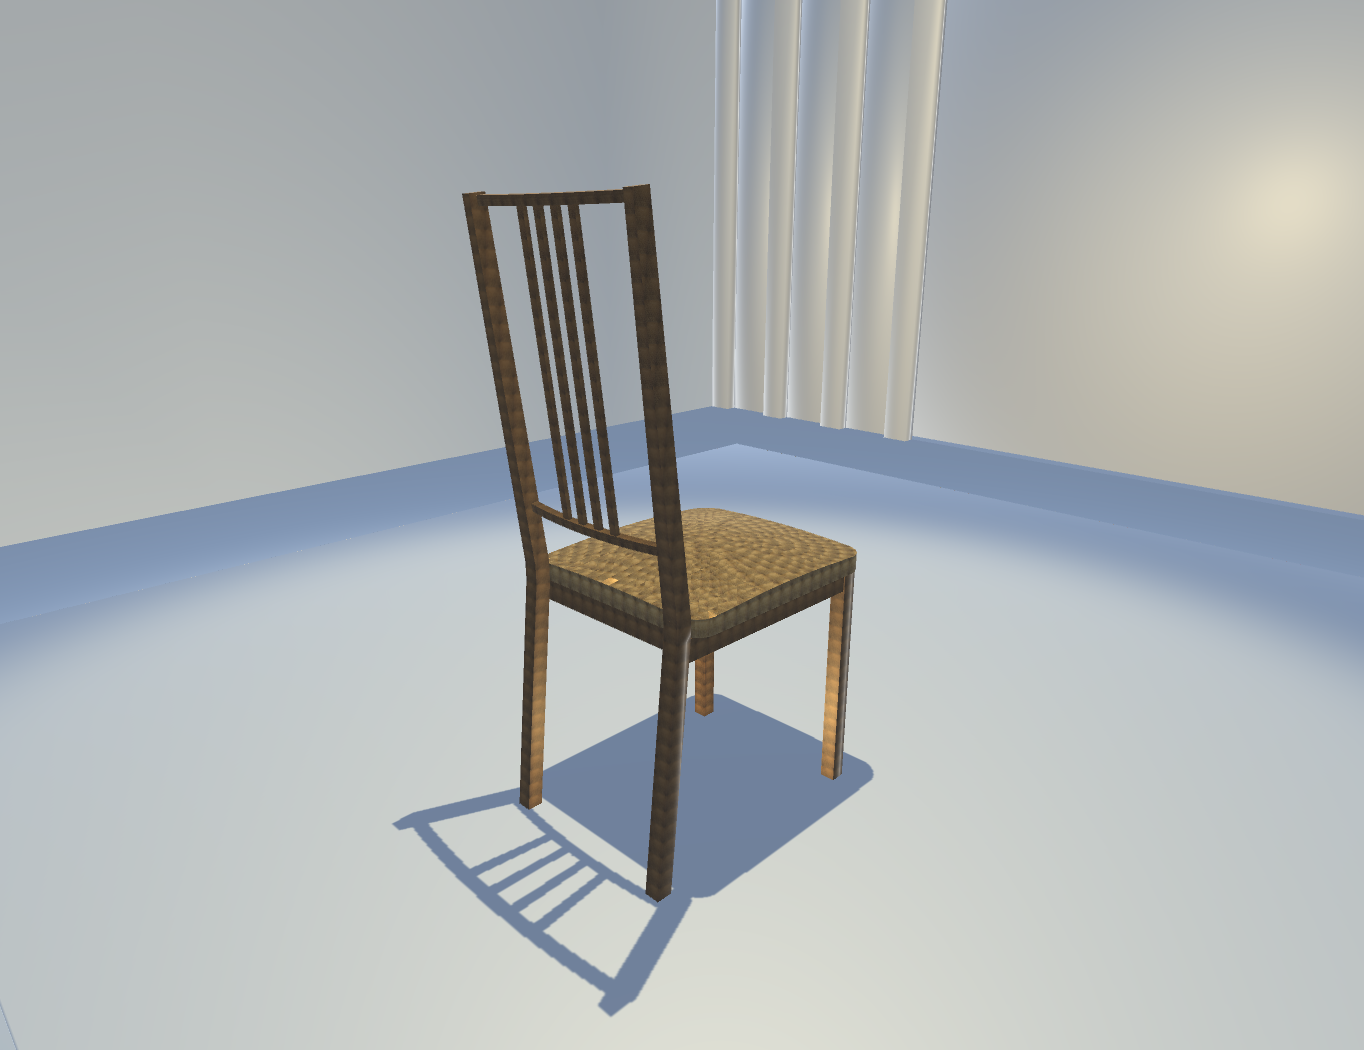
\includegraphics[width=.2\linewidth]{/Users/apple/OVGU/Thesis/code/3dReconstruction/report/images/evaluation/datasets/s2r_textureless_light_1} &
        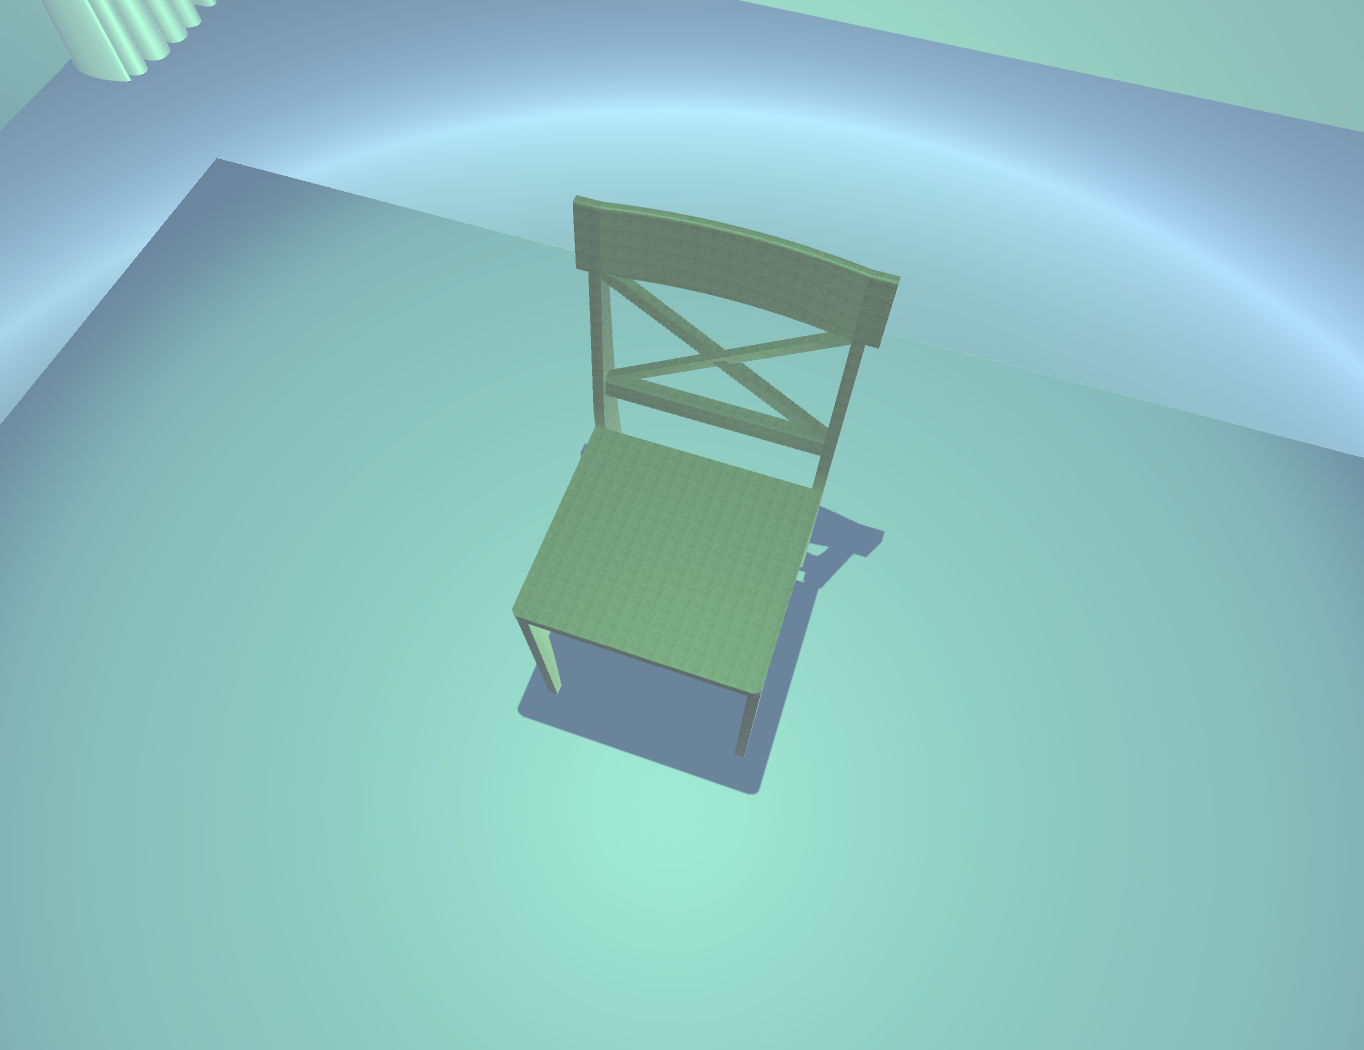
\includegraphics[width=.2\linewidth]{/Users/apple/OVGU/Thesis/code/3dReconstruction/report/images/evaluation/datasets/s2r_textureless_light_2} &
        \includegraphics[width=.2\linewidth]{/Users/apple/OVGU/Thesis/code/3dReconstruction/report/images/evaluation/datasets/s2r_textureless_light_3}\\

        Textured & \includegraphics[width=.2\linewidth]{/Users/apple/OVGU/Thesis/code/3dReconstruction/report/images/evaluation/datasets/s2r_textured_1} &
        \includegraphics[width=.2\linewidth]{/Users/apple/OVGU/Thesis/code/3dReconstruction/report/images/evaluation/datasets/s2r_textured_2} &
        \includegraphics[width=.2\linewidth]{/Users/apple/OVGU/Thesis/code/3dReconstruction/report/images/evaluation/datasets/s2r_textured_3}\\

        Textured with light & \includegraphics[width=.2\linewidth]{/Users/apple/OVGU/Thesis/code/3dReconstruction/report/images/evaluation/datasets/s2r_textured_light_1} &
        \includegraphics[width=.2\linewidth]{/Users/apple/OVGU/Thesis/code/3dReconstruction/report/images/evaluation/datasets/s2r_textured_light_2} &
        \includegraphics[width=.2\linewidth]{/Users/apple/OVGU/Thesis/code/3dReconstruction/report/images/evaluation/datasets/s2r_textured_light_4}\\

        Multi-Object & \includegraphics[width=.2\linewidth]{/Users/apple/OVGU/Thesis/code/3dReconstruction/report/images/evaluation/datasets/s2r_chair_1} &
        \includegraphics[width=.2\linewidth]{/Users/apple/OVGU/Thesis/code/3dReconstruction/report/images/evaluation/datasets/s2r_chair_2} &
        \includegraphics[width=.2\linewidth]{/Users/apple/OVGU/Thesis/code/3dReconstruction/report/images/evaluation/datasets/s2r_chair_3}\\

    \end{tabular}
    \caption[Samples for Datasets Used for Ablastion Study.]{Samples of images used for ablation study on chairs with different parameters of domain randomization.}
    \label{fig:domain_randomisation_for_ablation_study}
\end{figure}

%\begin{figure}
%    \centering
%    \resizebox{\textwidth}{!}{%% Creator: Matplotlib, PGF backend
%%
%% To include the figure in your LaTeX document, write
%%   \input{<filename>.pgf}
%%
%% Make sure the required packages are loaded in your preamble
%%   \usepackage{pgf}
%%
%% Figures using additional raster images can only be included by \input if
%% they are in the same directory as the main LaTeX file. For loading figures
%% from other directories you can use the `import` package
%%   \usepackage{import}
%%
%% and then include the figures with
%%   \import{<path to file>}{<filename>.pgf}
%%
%% Matplotlib used the following preamble
%%   \usepackage{fontspec}
%%   \setmainfont{DejaVuSerif.ttf}[Path=\detokenize{/Users/apple/opt/anaconda3/envs/kaolin/lib/python3.7/site-packages/matplotlib/mpl-data/fonts/ttf/}]
%%   \setsansfont{DejaVuSans.ttf}[Path=\detokenize{/Users/apple/opt/anaconda3/envs/kaolin/lib/python3.7/site-packages/matplotlib/mpl-data/fonts/ttf/}]
%%   \setmonofont{DejaVuSansMono.ttf}[Path=\detokenize{/Users/apple/opt/anaconda3/envs/kaolin/lib/python3.7/site-packages/matplotlib/mpl-data/fonts/ttf/}]
%%
\begingroup%
\makeatletter%
\begin{pgfpicture}%
\pgfpathrectangle{\pgfpointorigin}{\pgfqpoint{5.541978in}{4.337596in}}%
\pgfusepath{use as bounding box, clip}%
\begin{pgfscope}%
\pgfsetbuttcap%
\pgfsetmiterjoin%
\definecolor{currentfill}{rgb}{1.000000,1.000000,1.000000}%
\pgfsetfillcolor{currentfill}%
\pgfsetlinewidth{0.000000pt}%
\definecolor{currentstroke}{rgb}{1.000000,1.000000,1.000000}%
\pgfsetstrokecolor{currentstroke}%
\pgfsetdash{}{0pt}%
\pgfpathmoveto{\pgfqpoint{0.000000in}{0.000000in}}%
\pgfpathlineto{\pgfqpoint{5.541978in}{0.000000in}}%
\pgfpathlineto{\pgfqpoint{5.541978in}{4.337596in}}%
\pgfpathlineto{\pgfqpoint{0.000000in}{4.337596in}}%
\pgfpathclose%
\pgfusepath{fill}%
\end{pgfscope}%
\begin{pgfscope}%
\pgfsetbuttcap%
\pgfsetmiterjoin%
\definecolor{currentfill}{rgb}{1.000000,1.000000,1.000000}%
\pgfsetfillcolor{currentfill}%
\pgfsetlinewidth{0.000000pt}%
\definecolor{currentstroke}{rgb}{0.000000,0.000000,0.000000}%
\pgfsetstrokecolor{currentstroke}%
\pgfsetstrokeopacity{0.000000}%
\pgfsetdash{}{0pt}%
\pgfpathmoveto{\pgfqpoint{0.481978in}{0.331635in}}%
\pgfpathlineto{\pgfqpoint{5.441978in}{0.331635in}}%
\pgfpathlineto{\pgfqpoint{5.441978in}{4.027635in}}%
\pgfpathlineto{\pgfqpoint{0.481978in}{4.027635in}}%
\pgfpathclose%
\pgfusepath{fill}%
\end{pgfscope}%
\begin{pgfscope}%
\pgfpathrectangle{\pgfqpoint{0.481978in}{0.331635in}}{\pgfqpoint{4.960000in}{3.696000in}}%
\pgfusepath{clip}%
\pgfsetbuttcap%
\pgfsetroundjoin%
\definecolor{currentfill}{rgb}{1.000000,0.705882,0.509804}%
\pgfsetfillcolor{currentfill}%
\pgfsetlinewidth{0.481800pt}%
\definecolor{currentstroke}{rgb}{1.000000,1.000000,1.000000}%
\pgfsetstrokecolor{currentstroke}%
\pgfsetdash{}{0pt}%
\pgfpathmoveto{\pgfqpoint{3.360566in}{1.125291in}}%
\pgfpathcurveto{\pgfqpoint{3.371616in}{1.125291in}}{\pgfqpoint{3.382215in}{1.129681in}}{\pgfqpoint{3.390029in}{1.137495in}}%
\pgfpathcurveto{\pgfqpoint{3.397843in}{1.145309in}}{\pgfqpoint{3.402233in}{1.155908in}}{\pgfqpoint{3.402233in}{1.166958in}}%
\pgfpathcurveto{\pgfqpoint{3.402233in}{1.178008in}}{\pgfqpoint{3.397843in}{1.188607in}}{\pgfqpoint{3.390029in}{1.196421in}}%
\pgfpathcurveto{\pgfqpoint{3.382215in}{1.204234in}}{\pgfqpoint{3.371616in}{1.208624in}}{\pgfqpoint{3.360566in}{1.208624in}}%
\pgfpathcurveto{\pgfqpoint{3.349516in}{1.208624in}}{\pgfqpoint{3.338917in}{1.204234in}}{\pgfqpoint{3.331103in}{1.196421in}}%
\pgfpathcurveto{\pgfqpoint{3.323290in}{1.188607in}}{\pgfqpoint{3.318900in}{1.178008in}}{\pgfqpoint{3.318900in}{1.166958in}}%
\pgfpathcurveto{\pgfqpoint{3.318900in}{1.155908in}}{\pgfqpoint{3.323290in}{1.145309in}}{\pgfqpoint{3.331103in}{1.137495in}}%
\pgfpathcurveto{\pgfqpoint{3.338917in}{1.129681in}}{\pgfqpoint{3.349516in}{1.125291in}}{\pgfqpoint{3.360566in}{1.125291in}}%
\pgfpathclose%
\pgfusepath{stroke,fill}%
\end{pgfscope}%
\begin{pgfscope}%
\pgfpathrectangle{\pgfqpoint{0.481978in}{0.331635in}}{\pgfqpoint{4.960000in}{3.696000in}}%
\pgfusepath{clip}%
\pgfsetbuttcap%
\pgfsetroundjoin%
\definecolor{currentfill}{rgb}{1.000000,0.705882,0.509804}%
\pgfsetfillcolor{currentfill}%
\pgfsetlinewidth{0.481800pt}%
\definecolor{currentstroke}{rgb}{1.000000,1.000000,1.000000}%
\pgfsetstrokecolor{currentstroke}%
\pgfsetdash{}{0pt}%
\pgfpathmoveto{\pgfqpoint{2.551616in}{1.428387in}}%
\pgfpathcurveto{\pgfqpoint{2.562666in}{1.428387in}}{\pgfqpoint{2.573265in}{1.432777in}}{\pgfqpoint{2.581078in}{1.440591in}}%
\pgfpathcurveto{\pgfqpoint{2.588892in}{1.448404in}}{\pgfqpoint{2.593282in}{1.459003in}}{\pgfqpoint{2.593282in}{1.470054in}}%
\pgfpathcurveto{\pgfqpoint{2.593282in}{1.481104in}}{\pgfqpoint{2.588892in}{1.491703in}}{\pgfqpoint{2.581078in}{1.499516in}}%
\pgfpathcurveto{\pgfqpoint{2.573265in}{1.507330in}}{\pgfqpoint{2.562666in}{1.511720in}}{\pgfqpoint{2.551616in}{1.511720in}}%
\pgfpathcurveto{\pgfqpoint{2.540565in}{1.511720in}}{\pgfqpoint{2.529966in}{1.507330in}}{\pgfqpoint{2.522153in}{1.499516in}}%
\pgfpathcurveto{\pgfqpoint{2.514339in}{1.491703in}}{\pgfqpoint{2.509949in}{1.481104in}}{\pgfqpoint{2.509949in}{1.470054in}}%
\pgfpathcurveto{\pgfqpoint{2.509949in}{1.459003in}}{\pgfqpoint{2.514339in}{1.448404in}}{\pgfqpoint{2.522153in}{1.440591in}}%
\pgfpathcurveto{\pgfqpoint{2.529966in}{1.432777in}}{\pgfqpoint{2.540565in}{1.428387in}}{\pgfqpoint{2.551616in}{1.428387in}}%
\pgfpathclose%
\pgfusepath{stroke,fill}%
\end{pgfscope}%
\begin{pgfscope}%
\pgfpathrectangle{\pgfqpoint{0.481978in}{0.331635in}}{\pgfqpoint{4.960000in}{3.696000in}}%
\pgfusepath{clip}%
\pgfsetbuttcap%
\pgfsetroundjoin%
\definecolor{currentfill}{rgb}{1.000000,0.705882,0.509804}%
\pgfsetfillcolor{currentfill}%
\pgfsetlinewidth{0.481800pt}%
\definecolor{currentstroke}{rgb}{1.000000,1.000000,1.000000}%
\pgfsetstrokecolor{currentstroke}%
\pgfsetdash{}{0pt}%
\pgfpathmoveto{\pgfqpoint{2.399813in}{1.160374in}}%
\pgfpathcurveto{\pgfqpoint{2.410863in}{1.160374in}}{\pgfqpoint{2.421462in}{1.164764in}}{\pgfqpoint{2.429276in}{1.172578in}}%
\pgfpathcurveto{\pgfqpoint{2.437090in}{1.180392in}}{\pgfqpoint{2.441480in}{1.190991in}}{\pgfqpoint{2.441480in}{1.202041in}}%
\pgfpathcurveto{\pgfqpoint{2.441480in}{1.213091in}}{\pgfqpoint{2.437090in}{1.223690in}}{\pgfqpoint{2.429276in}{1.231504in}}%
\pgfpathcurveto{\pgfqpoint{2.421462in}{1.239317in}}{\pgfqpoint{2.410863in}{1.243708in}}{\pgfqpoint{2.399813in}{1.243708in}}%
\pgfpathcurveto{\pgfqpoint{2.388763in}{1.243708in}}{\pgfqpoint{2.378164in}{1.239317in}}{\pgfqpoint{2.370350in}{1.231504in}}%
\pgfpathcurveto{\pgfqpoint{2.362537in}{1.223690in}}{\pgfqpoint{2.358147in}{1.213091in}}{\pgfqpoint{2.358147in}{1.202041in}}%
\pgfpathcurveto{\pgfqpoint{2.358147in}{1.190991in}}{\pgfqpoint{2.362537in}{1.180392in}}{\pgfqpoint{2.370350in}{1.172578in}}%
\pgfpathcurveto{\pgfqpoint{2.378164in}{1.164764in}}{\pgfqpoint{2.388763in}{1.160374in}}{\pgfqpoint{2.399813in}{1.160374in}}%
\pgfpathclose%
\pgfusepath{stroke,fill}%
\end{pgfscope}%
\begin{pgfscope}%
\pgfpathrectangle{\pgfqpoint{0.481978in}{0.331635in}}{\pgfqpoint{4.960000in}{3.696000in}}%
\pgfusepath{clip}%
\pgfsetbuttcap%
\pgfsetroundjoin%
\definecolor{currentfill}{rgb}{1.000000,0.705882,0.509804}%
\pgfsetfillcolor{currentfill}%
\pgfsetlinewidth{0.481800pt}%
\definecolor{currentstroke}{rgb}{1.000000,1.000000,1.000000}%
\pgfsetstrokecolor{currentstroke}%
\pgfsetdash{}{0pt}%
\pgfpathmoveto{\pgfqpoint{2.286581in}{0.772010in}}%
\pgfpathcurveto{\pgfqpoint{2.297631in}{0.772010in}}{\pgfqpoint{2.308230in}{0.776400in}}{\pgfqpoint{2.316044in}{0.784214in}}%
\pgfpathcurveto{\pgfqpoint{2.323858in}{0.792027in}}{\pgfqpoint{2.328248in}{0.802626in}}{\pgfqpoint{2.328248in}{0.813677in}}%
\pgfpathcurveto{\pgfqpoint{2.328248in}{0.824727in}}{\pgfqpoint{2.323858in}{0.835326in}}{\pgfqpoint{2.316044in}{0.843139in}}%
\pgfpathcurveto{\pgfqpoint{2.308230in}{0.850953in}}{\pgfqpoint{2.297631in}{0.855343in}}{\pgfqpoint{2.286581in}{0.855343in}}%
\pgfpathcurveto{\pgfqpoint{2.275531in}{0.855343in}}{\pgfqpoint{2.264932in}{0.850953in}}{\pgfqpoint{2.257119in}{0.843139in}}%
\pgfpathcurveto{\pgfqpoint{2.249305in}{0.835326in}}{\pgfqpoint{2.244915in}{0.824727in}}{\pgfqpoint{2.244915in}{0.813677in}}%
\pgfpathcurveto{\pgfqpoint{2.244915in}{0.802626in}}{\pgfqpoint{2.249305in}{0.792027in}}{\pgfqpoint{2.257119in}{0.784214in}}%
\pgfpathcurveto{\pgfqpoint{2.264932in}{0.776400in}}{\pgfqpoint{2.275531in}{0.772010in}}{\pgfqpoint{2.286581in}{0.772010in}}%
\pgfpathclose%
\pgfusepath{stroke,fill}%
\end{pgfscope}%
\begin{pgfscope}%
\pgfpathrectangle{\pgfqpoint{0.481978in}{0.331635in}}{\pgfqpoint{4.960000in}{3.696000in}}%
\pgfusepath{clip}%
\pgfsetbuttcap%
\pgfsetroundjoin%
\definecolor{currentfill}{rgb}{1.000000,0.705882,0.509804}%
\pgfsetfillcolor{currentfill}%
\pgfsetlinewidth{0.481800pt}%
\definecolor{currentstroke}{rgb}{1.000000,1.000000,1.000000}%
\pgfsetstrokecolor{currentstroke}%
\pgfsetdash{}{0pt}%
\pgfpathmoveto{\pgfqpoint{0.861902in}{2.271937in}}%
\pgfpathcurveto{\pgfqpoint{0.872952in}{2.271937in}}{\pgfqpoint{0.883551in}{2.276327in}}{\pgfqpoint{0.891365in}{2.284141in}}%
\pgfpathcurveto{\pgfqpoint{0.899178in}{2.291955in}}{\pgfqpoint{0.903569in}{2.302554in}}{\pgfqpoint{0.903569in}{2.313604in}}%
\pgfpathcurveto{\pgfqpoint{0.903569in}{2.324654in}}{\pgfqpoint{0.899178in}{2.335253in}}{\pgfqpoint{0.891365in}{2.343067in}}%
\pgfpathcurveto{\pgfqpoint{0.883551in}{2.350880in}}{\pgfqpoint{0.872952in}{2.355270in}}{\pgfqpoint{0.861902in}{2.355270in}}%
\pgfpathcurveto{\pgfqpoint{0.850852in}{2.355270in}}{\pgfqpoint{0.840253in}{2.350880in}}{\pgfqpoint{0.832439in}{2.343067in}}%
\pgfpathcurveto{\pgfqpoint{0.824626in}{2.335253in}}{\pgfqpoint{0.820235in}{2.324654in}}{\pgfqpoint{0.820235in}{2.313604in}}%
\pgfpathcurveto{\pgfqpoint{0.820235in}{2.302554in}}{\pgfqpoint{0.824626in}{2.291955in}}{\pgfqpoint{0.832439in}{2.284141in}}%
\pgfpathcurveto{\pgfqpoint{0.840253in}{2.276327in}}{\pgfqpoint{0.850852in}{2.271937in}}{\pgfqpoint{0.861902in}{2.271937in}}%
\pgfpathclose%
\pgfusepath{stroke,fill}%
\end{pgfscope}%
\begin{pgfscope}%
\pgfpathrectangle{\pgfqpoint{0.481978in}{0.331635in}}{\pgfqpoint{4.960000in}{3.696000in}}%
\pgfusepath{clip}%
\pgfsetbuttcap%
\pgfsetroundjoin%
\definecolor{currentfill}{rgb}{1.000000,0.705882,0.509804}%
\pgfsetfillcolor{currentfill}%
\pgfsetlinewidth{0.481800pt}%
\definecolor{currentstroke}{rgb}{1.000000,1.000000,1.000000}%
\pgfsetstrokecolor{currentstroke}%
\pgfsetdash{}{0pt}%
\pgfpathmoveto{\pgfqpoint{1.334421in}{1.323680in}}%
\pgfpathcurveto{\pgfqpoint{1.345472in}{1.323680in}}{\pgfqpoint{1.356071in}{1.328070in}}{\pgfqpoint{1.363884in}{1.335884in}}%
\pgfpathcurveto{\pgfqpoint{1.371698in}{1.343697in}}{\pgfqpoint{1.376088in}{1.354296in}}{\pgfqpoint{1.376088in}{1.365347in}}%
\pgfpathcurveto{\pgfqpoint{1.376088in}{1.376397in}}{\pgfqpoint{1.371698in}{1.386996in}}{\pgfqpoint{1.363884in}{1.394809in}}%
\pgfpathcurveto{\pgfqpoint{1.356071in}{1.402623in}}{\pgfqpoint{1.345472in}{1.407013in}}{\pgfqpoint{1.334421in}{1.407013in}}%
\pgfpathcurveto{\pgfqpoint{1.323371in}{1.407013in}}{\pgfqpoint{1.312772in}{1.402623in}}{\pgfqpoint{1.304959in}{1.394809in}}%
\pgfpathcurveto{\pgfqpoint{1.297145in}{1.386996in}}{\pgfqpoint{1.292755in}{1.376397in}}{\pgfqpoint{1.292755in}{1.365347in}}%
\pgfpathcurveto{\pgfqpoint{1.292755in}{1.354296in}}{\pgfqpoint{1.297145in}{1.343697in}}{\pgfqpoint{1.304959in}{1.335884in}}%
\pgfpathcurveto{\pgfqpoint{1.312772in}{1.328070in}}{\pgfqpoint{1.323371in}{1.323680in}}{\pgfqpoint{1.334421in}{1.323680in}}%
\pgfpathclose%
\pgfusepath{stroke,fill}%
\end{pgfscope}%
\begin{pgfscope}%
\pgfpathrectangle{\pgfqpoint{0.481978in}{0.331635in}}{\pgfqpoint{4.960000in}{3.696000in}}%
\pgfusepath{clip}%
\pgfsetbuttcap%
\pgfsetroundjoin%
\definecolor{currentfill}{rgb}{1.000000,0.705882,0.509804}%
\pgfsetfillcolor{currentfill}%
\pgfsetlinewidth{0.481800pt}%
\definecolor{currentstroke}{rgb}{1.000000,1.000000,1.000000}%
\pgfsetstrokecolor{currentstroke}%
\pgfsetdash{}{0pt}%
\pgfpathmoveto{\pgfqpoint{1.463739in}{1.377709in}}%
\pgfpathcurveto{\pgfqpoint{1.474789in}{1.377709in}}{\pgfqpoint{1.485388in}{1.382099in}}{\pgfqpoint{1.493202in}{1.389913in}}%
\pgfpathcurveto{\pgfqpoint{1.501015in}{1.397726in}}{\pgfqpoint{1.505406in}{1.408325in}}{\pgfqpoint{1.505406in}{1.419375in}}%
\pgfpathcurveto{\pgfqpoint{1.505406in}{1.430426in}}{\pgfqpoint{1.501015in}{1.441025in}}{\pgfqpoint{1.493202in}{1.448838in}}%
\pgfpathcurveto{\pgfqpoint{1.485388in}{1.456652in}}{\pgfqpoint{1.474789in}{1.461042in}}{\pgfqpoint{1.463739in}{1.461042in}}%
\pgfpathcurveto{\pgfqpoint{1.452689in}{1.461042in}}{\pgfqpoint{1.442090in}{1.456652in}}{\pgfqpoint{1.434276in}{1.448838in}}%
\pgfpathcurveto{\pgfqpoint{1.426463in}{1.441025in}}{\pgfqpoint{1.422072in}{1.430426in}}{\pgfqpoint{1.422072in}{1.419375in}}%
\pgfpathcurveto{\pgfqpoint{1.422072in}{1.408325in}}{\pgfqpoint{1.426463in}{1.397726in}}{\pgfqpoint{1.434276in}{1.389913in}}%
\pgfpathcurveto{\pgfqpoint{1.442090in}{1.382099in}}{\pgfqpoint{1.452689in}{1.377709in}}{\pgfqpoint{1.463739in}{1.377709in}}%
\pgfpathclose%
\pgfusepath{stroke,fill}%
\end{pgfscope}%
\begin{pgfscope}%
\pgfpathrectangle{\pgfqpoint{0.481978in}{0.331635in}}{\pgfqpoint{4.960000in}{3.696000in}}%
\pgfusepath{clip}%
\pgfsetbuttcap%
\pgfsetroundjoin%
\definecolor{currentfill}{rgb}{1.000000,0.705882,0.509804}%
\pgfsetfillcolor{currentfill}%
\pgfsetlinewidth{0.481800pt}%
\definecolor{currentstroke}{rgb}{1.000000,1.000000,1.000000}%
\pgfsetstrokecolor{currentstroke}%
\pgfsetdash{}{0pt}%
\pgfpathmoveto{\pgfqpoint{1.694579in}{2.220657in}}%
\pgfpathcurveto{\pgfqpoint{1.705629in}{2.220657in}}{\pgfqpoint{1.716228in}{2.225047in}}{\pgfqpoint{1.724042in}{2.232860in}}%
\pgfpathcurveto{\pgfqpoint{1.731856in}{2.240674in}}{\pgfqpoint{1.736246in}{2.251273in}}{\pgfqpoint{1.736246in}{2.262323in}}%
\pgfpathcurveto{\pgfqpoint{1.736246in}{2.273373in}}{\pgfqpoint{1.731856in}{2.283972in}}{\pgfqpoint{1.724042in}{2.291786in}}%
\pgfpathcurveto{\pgfqpoint{1.716228in}{2.299600in}}{\pgfqpoint{1.705629in}{2.303990in}}{\pgfqpoint{1.694579in}{2.303990in}}%
\pgfpathcurveto{\pgfqpoint{1.683529in}{2.303990in}}{\pgfqpoint{1.672930in}{2.299600in}}{\pgfqpoint{1.665116in}{2.291786in}}%
\pgfpathcurveto{\pgfqpoint{1.657303in}{2.283972in}}{\pgfqpoint{1.652913in}{2.273373in}}{\pgfqpoint{1.652913in}{2.262323in}}%
\pgfpathcurveto{\pgfqpoint{1.652913in}{2.251273in}}{\pgfqpoint{1.657303in}{2.240674in}}{\pgfqpoint{1.665116in}{2.232860in}}%
\pgfpathcurveto{\pgfqpoint{1.672930in}{2.225047in}}{\pgfqpoint{1.683529in}{2.220657in}}{\pgfqpoint{1.694579in}{2.220657in}}%
\pgfpathclose%
\pgfusepath{stroke,fill}%
\end{pgfscope}%
\begin{pgfscope}%
\pgfpathrectangle{\pgfqpoint{0.481978in}{0.331635in}}{\pgfqpoint{4.960000in}{3.696000in}}%
\pgfusepath{clip}%
\pgfsetbuttcap%
\pgfsetroundjoin%
\definecolor{currentfill}{rgb}{1.000000,0.705882,0.509804}%
\pgfsetfillcolor{currentfill}%
\pgfsetlinewidth{0.481800pt}%
\definecolor{currentstroke}{rgb}{1.000000,1.000000,1.000000}%
\pgfsetstrokecolor{currentstroke}%
\pgfsetdash{}{0pt}%
\pgfpathmoveto{\pgfqpoint{2.769947in}{1.566760in}}%
\pgfpathcurveto{\pgfqpoint{2.780997in}{1.566760in}}{\pgfqpoint{2.791596in}{1.571150in}}{\pgfqpoint{2.799410in}{1.578964in}}%
\pgfpathcurveto{\pgfqpoint{2.807223in}{1.586777in}}{\pgfqpoint{2.811613in}{1.597376in}}{\pgfqpoint{2.811613in}{1.608426in}}%
\pgfpathcurveto{\pgfqpoint{2.811613in}{1.619477in}}{\pgfqpoint{2.807223in}{1.630076in}}{\pgfqpoint{2.799410in}{1.637889in}}%
\pgfpathcurveto{\pgfqpoint{2.791596in}{1.645703in}}{\pgfqpoint{2.780997in}{1.650093in}}{\pgfqpoint{2.769947in}{1.650093in}}%
\pgfpathcurveto{\pgfqpoint{2.758897in}{1.650093in}}{\pgfqpoint{2.748298in}{1.645703in}}{\pgfqpoint{2.740484in}{1.637889in}}%
\pgfpathcurveto{\pgfqpoint{2.732670in}{1.630076in}}{\pgfqpoint{2.728280in}{1.619477in}}{\pgfqpoint{2.728280in}{1.608426in}}%
\pgfpathcurveto{\pgfqpoint{2.728280in}{1.597376in}}{\pgfqpoint{2.732670in}{1.586777in}}{\pgfqpoint{2.740484in}{1.578964in}}%
\pgfpathcurveto{\pgfqpoint{2.748298in}{1.571150in}}{\pgfqpoint{2.758897in}{1.566760in}}{\pgfqpoint{2.769947in}{1.566760in}}%
\pgfpathclose%
\pgfusepath{stroke,fill}%
\end{pgfscope}%
\begin{pgfscope}%
\pgfpathrectangle{\pgfqpoint{0.481978in}{0.331635in}}{\pgfqpoint{4.960000in}{3.696000in}}%
\pgfusepath{clip}%
\pgfsetbuttcap%
\pgfsetroundjoin%
\definecolor{currentfill}{rgb}{1.000000,0.705882,0.509804}%
\pgfsetfillcolor{currentfill}%
\pgfsetlinewidth{0.481800pt}%
\definecolor{currentstroke}{rgb}{1.000000,1.000000,1.000000}%
\pgfsetstrokecolor{currentstroke}%
\pgfsetdash{}{0pt}%
\pgfpathmoveto{\pgfqpoint{1.635810in}{0.831188in}}%
\pgfpathcurveto{\pgfqpoint{1.646860in}{0.831188in}}{\pgfqpoint{1.657459in}{0.835579in}}{\pgfqpoint{1.665273in}{0.843392in}}%
\pgfpathcurveto{\pgfqpoint{1.673087in}{0.851206in}}{\pgfqpoint{1.677477in}{0.861805in}}{\pgfqpoint{1.677477in}{0.872855in}}%
\pgfpathcurveto{\pgfqpoint{1.677477in}{0.883905in}}{\pgfqpoint{1.673087in}{0.894504in}}{\pgfqpoint{1.665273in}{0.902318in}}%
\pgfpathcurveto{\pgfqpoint{1.657459in}{0.910131in}}{\pgfqpoint{1.646860in}{0.914522in}}{\pgfqpoint{1.635810in}{0.914522in}}%
\pgfpathcurveto{\pgfqpoint{1.624760in}{0.914522in}}{\pgfqpoint{1.614161in}{0.910131in}}{\pgfqpoint{1.606347in}{0.902318in}}%
\pgfpathcurveto{\pgfqpoint{1.598534in}{0.894504in}}{\pgfqpoint{1.594144in}{0.883905in}}{\pgfqpoint{1.594144in}{0.872855in}}%
\pgfpathcurveto{\pgfqpoint{1.594144in}{0.861805in}}{\pgfqpoint{1.598534in}{0.851206in}}{\pgfqpoint{1.606347in}{0.843392in}}%
\pgfpathcurveto{\pgfqpoint{1.614161in}{0.835579in}}{\pgfqpoint{1.624760in}{0.831188in}}{\pgfqpoint{1.635810in}{0.831188in}}%
\pgfpathclose%
\pgfusepath{stroke,fill}%
\end{pgfscope}%
\begin{pgfscope}%
\pgfpathrectangle{\pgfqpoint{0.481978in}{0.331635in}}{\pgfqpoint{4.960000in}{3.696000in}}%
\pgfusepath{clip}%
\pgfsetbuttcap%
\pgfsetroundjoin%
\definecolor{currentfill}{rgb}{1.000000,0.705882,0.509804}%
\pgfsetfillcolor{currentfill}%
\pgfsetlinewidth{0.481800pt}%
\definecolor{currentstroke}{rgb}{1.000000,1.000000,1.000000}%
\pgfsetstrokecolor{currentstroke}%
\pgfsetdash{}{0pt}%
\pgfpathmoveto{\pgfqpoint{0.864107in}{1.651059in}}%
\pgfpathcurveto{\pgfqpoint{0.875157in}{1.651059in}}{\pgfqpoint{0.885756in}{1.655449in}}{\pgfqpoint{0.893570in}{1.663263in}}%
\pgfpathcurveto{\pgfqpoint{0.901383in}{1.671076in}}{\pgfqpoint{0.905773in}{1.681675in}}{\pgfqpoint{0.905773in}{1.692725in}}%
\pgfpathcurveto{\pgfqpoint{0.905773in}{1.703776in}}{\pgfqpoint{0.901383in}{1.714375in}}{\pgfqpoint{0.893570in}{1.722188in}}%
\pgfpathcurveto{\pgfqpoint{0.885756in}{1.730002in}}{\pgfqpoint{0.875157in}{1.734392in}}{\pgfqpoint{0.864107in}{1.734392in}}%
\pgfpathcurveto{\pgfqpoint{0.853057in}{1.734392in}}{\pgfqpoint{0.842458in}{1.730002in}}{\pgfqpoint{0.834644in}{1.722188in}}%
\pgfpathcurveto{\pgfqpoint{0.826830in}{1.714375in}}{\pgfqpoint{0.822440in}{1.703776in}}{\pgfqpoint{0.822440in}{1.692725in}}%
\pgfpathcurveto{\pgfqpoint{0.822440in}{1.681675in}}{\pgfqpoint{0.826830in}{1.671076in}}{\pgfqpoint{0.834644in}{1.663263in}}%
\pgfpathcurveto{\pgfqpoint{0.842458in}{1.655449in}}{\pgfqpoint{0.853057in}{1.651059in}}{\pgfqpoint{0.864107in}{1.651059in}}%
\pgfpathclose%
\pgfusepath{stroke,fill}%
\end{pgfscope}%
\begin{pgfscope}%
\pgfpathrectangle{\pgfqpoint{0.481978in}{0.331635in}}{\pgfqpoint{4.960000in}{3.696000in}}%
\pgfusepath{clip}%
\pgfsetbuttcap%
\pgfsetroundjoin%
\definecolor{currentfill}{rgb}{1.000000,0.705882,0.509804}%
\pgfsetfillcolor{currentfill}%
\pgfsetlinewidth{0.481800pt}%
\definecolor{currentstroke}{rgb}{1.000000,1.000000,1.000000}%
\pgfsetstrokecolor{currentstroke}%
\pgfsetdash{}{0pt}%
\pgfpathmoveto{\pgfqpoint{3.056141in}{0.869562in}}%
\pgfpathcurveto{\pgfqpoint{3.067192in}{0.869562in}}{\pgfqpoint{3.077791in}{0.873952in}}{\pgfqpoint{3.085604in}{0.881766in}}%
\pgfpathcurveto{\pgfqpoint{3.093418in}{0.889579in}}{\pgfqpoint{3.097808in}{0.900178in}}{\pgfqpoint{3.097808in}{0.911229in}}%
\pgfpathcurveto{\pgfqpoint{3.097808in}{0.922279in}}{\pgfqpoint{3.093418in}{0.932878in}}{\pgfqpoint{3.085604in}{0.940691in}}%
\pgfpathcurveto{\pgfqpoint{3.077791in}{0.948505in}}{\pgfqpoint{3.067192in}{0.952895in}}{\pgfqpoint{3.056141in}{0.952895in}}%
\pgfpathcurveto{\pgfqpoint{3.045091in}{0.952895in}}{\pgfqpoint{3.034492in}{0.948505in}}{\pgfqpoint{3.026679in}{0.940691in}}%
\pgfpathcurveto{\pgfqpoint{3.018865in}{0.932878in}}{\pgfqpoint{3.014475in}{0.922279in}}{\pgfqpoint{3.014475in}{0.911229in}}%
\pgfpathcurveto{\pgfqpoint{3.014475in}{0.900178in}}{\pgfqpoint{3.018865in}{0.889579in}}{\pgfqpoint{3.026679in}{0.881766in}}%
\pgfpathcurveto{\pgfqpoint{3.034492in}{0.873952in}}{\pgfqpoint{3.045091in}{0.869562in}}{\pgfqpoint{3.056141in}{0.869562in}}%
\pgfpathclose%
\pgfusepath{stroke,fill}%
\end{pgfscope}%
\begin{pgfscope}%
\pgfpathrectangle{\pgfqpoint{0.481978in}{0.331635in}}{\pgfqpoint{4.960000in}{3.696000in}}%
\pgfusepath{clip}%
\pgfsetbuttcap%
\pgfsetroundjoin%
\definecolor{currentfill}{rgb}{1.000000,0.705882,0.509804}%
\pgfsetfillcolor{currentfill}%
\pgfsetlinewidth{0.481800pt}%
\definecolor{currentstroke}{rgb}{1.000000,1.000000,1.000000}%
\pgfsetstrokecolor{currentstroke}%
\pgfsetdash{}{0pt}%
\pgfpathmoveto{\pgfqpoint{2.484228in}{3.145905in}}%
\pgfpathcurveto{\pgfqpoint{2.495278in}{3.145905in}}{\pgfqpoint{2.505877in}{3.150296in}}{\pgfqpoint{2.513691in}{3.158109in}}%
\pgfpathcurveto{\pgfqpoint{2.521505in}{3.165923in}}{\pgfqpoint{2.525895in}{3.176522in}}{\pgfqpoint{2.525895in}{3.187572in}}%
\pgfpathcurveto{\pgfqpoint{2.525895in}{3.198622in}}{\pgfqpoint{2.521505in}{3.209221in}}{\pgfqpoint{2.513691in}{3.217035in}}%
\pgfpathcurveto{\pgfqpoint{2.505877in}{3.224849in}}{\pgfqpoint{2.495278in}{3.229239in}}{\pgfqpoint{2.484228in}{3.229239in}}%
\pgfpathcurveto{\pgfqpoint{2.473178in}{3.229239in}}{\pgfqpoint{2.462579in}{3.224849in}}{\pgfqpoint{2.454765in}{3.217035in}}%
\pgfpathcurveto{\pgfqpoint{2.446952in}{3.209221in}}{\pgfqpoint{2.442562in}{3.198622in}}{\pgfqpoint{2.442562in}{3.187572in}}%
\pgfpathcurveto{\pgfqpoint{2.442562in}{3.176522in}}{\pgfqpoint{2.446952in}{3.165923in}}{\pgfqpoint{2.454765in}{3.158109in}}%
\pgfpathcurveto{\pgfqpoint{2.462579in}{3.150296in}}{\pgfqpoint{2.473178in}{3.145905in}}{\pgfqpoint{2.484228in}{3.145905in}}%
\pgfpathclose%
\pgfusepath{stroke,fill}%
\end{pgfscope}%
\begin{pgfscope}%
\pgfpathrectangle{\pgfqpoint{0.481978in}{0.331635in}}{\pgfqpoint{4.960000in}{3.696000in}}%
\pgfusepath{clip}%
\pgfsetbuttcap%
\pgfsetroundjoin%
\definecolor{currentfill}{rgb}{1.000000,0.705882,0.509804}%
\pgfsetfillcolor{currentfill}%
\pgfsetlinewidth{0.481800pt}%
\definecolor{currentstroke}{rgb}{1.000000,1.000000,1.000000}%
\pgfsetstrokecolor{currentstroke}%
\pgfsetdash{}{0pt}%
\pgfpathmoveto{\pgfqpoint{2.937021in}{1.957926in}}%
\pgfpathcurveto{\pgfqpoint{2.948071in}{1.957926in}}{\pgfqpoint{2.958670in}{1.962316in}}{\pgfqpoint{2.966484in}{1.970129in}}%
\pgfpathcurveto{\pgfqpoint{2.974298in}{1.977943in}}{\pgfqpoint{2.978688in}{1.988542in}}{\pgfqpoint{2.978688in}{1.999592in}}%
\pgfpathcurveto{\pgfqpoint{2.978688in}{2.010642in}}{\pgfqpoint{2.974298in}{2.021241in}}{\pgfqpoint{2.966484in}{2.029055in}}%
\pgfpathcurveto{\pgfqpoint{2.958670in}{2.036869in}}{\pgfqpoint{2.948071in}{2.041259in}}{\pgfqpoint{2.937021in}{2.041259in}}%
\pgfpathcurveto{\pgfqpoint{2.925971in}{2.041259in}}{\pgfqpoint{2.915372in}{2.036869in}}{\pgfqpoint{2.907558in}{2.029055in}}%
\pgfpathcurveto{\pgfqpoint{2.899745in}{2.021241in}}{\pgfqpoint{2.895354in}{2.010642in}}{\pgfqpoint{2.895354in}{1.999592in}}%
\pgfpathcurveto{\pgfqpoint{2.895354in}{1.988542in}}{\pgfqpoint{2.899745in}{1.977943in}}{\pgfqpoint{2.907558in}{1.970129in}}%
\pgfpathcurveto{\pgfqpoint{2.915372in}{1.962316in}}{\pgfqpoint{2.925971in}{1.957926in}}{\pgfqpoint{2.937021in}{1.957926in}}%
\pgfpathclose%
\pgfusepath{stroke,fill}%
\end{pgfscope}%
\begin{pgfscope}%
\pgfpathrectangle{\pgfqpoint{0.481978in}{0.331635in}}{\pgfqpoint{4.960000in}{3.696000in}}%
\pgfusepath{clip}%
\pgfsetbuttcap%
\pgfsetroundjoin%
\definecolor{currentfill}{rgb}{1.000000,0.705882,0.509804}%
\pgfsetfillcolor{currentfill}%
\pgfsetlinewidth{0.481800pt}%
\definecolor{currentstroke}{rgb}{1.000000,1.000000,1.000000}%
\pgfsetstrokecolor{currentstroke}%
\pgfsetdash{}{0pt}%
\pgfpathmoveto{\pgfqpoint{2.148348in}{0.708936in}}%
\pgfpathcurveto{\pgfqpoint{2.159398in}{0.708936in}}{\pgfqpoint{2.169997in}{0.713326in}}{\pgfqpoint{2.177811in}{0.721139in}}%
\pgfpathcurveto{\pgfqpoint{2.185625in}{0.728953in}}{\pgfqpoint{2.190015in}{0.739552in}}{\pgfqpoint{2.190015in}{0.750602in}}%
\pgfpathcurveto{\pgfqpoint{2.190015in}{0.761652in}}{\pgfqpoint{2.185625in}{0.772251in}}{\pgfqpoint{2.177811in}{0.780065in}}%
\pgfpathcurveto{\pgfqpoint{2.169997in}{0.787879in}}{\pgfqpoint{2.159398in}{0.792269in}}{\pgfqpoint{2.148348in}{0.792269in}}%
\pgfpathcurveto{\pgfqpoint{2.137298in}{0.792269in}}{\pgfqpoint{2.126699in}{0.787879in}}{\pgfqpoint{2.118886in}{0.780065in}}%
\pgfpathcurveto{\pgfqpoint{2.111072in}{0.772251in}}{\pgfqpoint{2.106682in}{0.761652in}}{\pgfqpoint{2.106682in}{0.750602in}}%
\pgfpathcurveto{\pgfqpoint{2.106682in}{0.739552in}}{\pgfqpoint{2.111072in}{0.728953in}}{\pgfqpoint{2.118886in}{0.721139in}}%
\pgfpathcurveto{\pgfqpoint{2.126699in}{0.713326in}}{\pgfqpoint{2.137298in}{0.708936in}}{\pgfqpoint{2.148348in}{0.708936in}}%
\pgfpathclose%
\pgfusepath{stroke,fill}%
\end{pgfscope}%
\begin{pgfscope}%
\pgfpathrectangle{\pgfqpoint{0.481978in}{0.331635in}}{\pgfqpoint{4.960000in}{3.696000in}}%
\pgfusepath{clip}%
\pgfsetbuttcap%
\pgfsetroundjoin%
\definecolor{currentfill}{rgb}{1.000000,0.705882,0.509804}%
\pgfsetfillcolor{currentfill}%
\pgfsetlinewidth{0.481800pt}%
\definecolor{currentstroke}{rgb}{1.000000,1.000000,1.000000}%
\pgfsetstrokecolor{currentstroke}%
\pgfsetdash{}{0pt}%
\pgfpathmoveto{\pgfqpoint{2.462547in}{3.333709in}}%
\pgfpathcurveto{\pgfqpoint{2.473597in}{3.333709in}}{\pgfqpoint{2.484196in}{3.338100in}}{\pgfqpoint{2.492009in}{3.345913in}}%
\pgfpathcurveto{\pgfqpoint{2.499823in}{3.353727in}}{\pgfqpoint{2.504213in}{3.364326in}}{\pgfqpoint{2.504213in}{3.375376in}}%
\pgfpathcurveto{\pgfqpoint{2.504213in}{3.386426in}}{\pgfqpoint{2.499823in}{3.397025in}}{\pgfqpoint{2.492009in}{3.404839in}}%
\pgfpathcurveto{\pgfqpoint{2.484196in}{3.412652in}}{\pgfqpoint{2.473597in}{3.417043in}}{\pgfqpoint{2.462547in}{3.417043in}}%
\pgfpathcurveto{\pgfqpoint{2.451497in}{3.417043in}}{\pgfqpoint{2.440897in}{3.412652in}}{\pgfqpoint{2.433084in}{3.404839in}}%
\pgfpathcurveto{\pgfqpoint{2.425270in}{3.397025in}}{\pgfqpoint{2.420880in}{3.386426in}}{\pgfqpoint{2.420880in}{3.375376in}}%
\pgfpathcurveto{\pgfqpoint{2.420880in}{3.364326in}}{\pgfqpoint{2.425270in}{3.353727in}}{\pgfqpoint{2.433084in}{3.345913in}}%
\pgfpathcurveto{\pgfqpoint{2.440897in}{3.338100in}}{\pgfqpoint{2.451497in}{3.333709in}}{\pgfqpoint{2.462547in}{3.333709in}}%
\pgfpathclose%
\pgfusepath{stroke,fill}%
\end{pgfscope}%
\begin{pgfscope}%
\pgfpathrectangle{\pgfqpoint{0.481978in}{0.331635in}}{\pgfqpoint{4.960000in}{3.696000in}}%
\pgfusepath{clip}%
\pgfsetbuttcap%
\pgfsetroundjoin%
\definecolor{currentfill}{rgb}{1.000000,0.705882,0.509804}%
\pgfsetfillcolor{currentfill}%
\pgfsetlinewidth{0.481800pt}%
\definecolor{currentstroke}{rgb}{1.000000,1.000000,1.000000}%
\pgfsetstrokecolor{currentstroke}%
\pgfsetdash{}{0pt}%
\pgfpathmoveto{\pgfqpoint{2.336175in}{1.326231in}}%
\pgfpathcurveto{\pgfqpoint{2.347225in}{1.326231in}}{\pgfqpoint{2.357824in}{1.330621in}}{\pgfqpoint{2.365637in}{1.338435in}}%
\pgfpathcurveto{\pgfqpoint{2.373451in}{1.346248in}}{\pgfqpoint{2.377841in}{1.356847in}}{\pgfqpoint{2.377841in}{1.367898in}}%
\pgfpathcurveto{\pgfqpoint{2.377841in}{1.378948in}}{\pgfqpoint{2.373451in}{1.389547in}}{\pgfqpoint{2.365637in}{1.397360in}}%
\pgfpathcurveto{\pgfqpoint{2.357824in}{1.405174in}}{\pgfqpoint{2.347225in}{1.409564in}}{\pgfqpoint{2.336175in}{1.409564in}}%
\pgfpathcurveto{\pgfqpoint{2.325124in}{1.409564in}}{\pgfqpoint{2.314525in}{1.405174in}}{\pgfqpoint{2.306712in}{1.397360in}}%
\pgfpathcurveto{\pgfqpoint{2.298898in}{1.389547in}}{\pgfqpoint{2.294508in}{1.378948in}}{\pgfqpoint{2.294508in}{1.367898in}}%
\pgfpathcurveto{\pgfqpoint{2.294508in}{1.356847in}}{\pgfqpoint{2.298898in}{1.346248in}}{\pgfqpoint{2.306712in}{1.338435in}}%
\pgfpathcurveto{\pgfqpoint{2.314525in}{1.330621in}}{\pgfqpoint{2.325124in}{1.326231in}}{\pgfqpoint{2.336175in}{1.326231in}}%
\pgfpathclose%
\pgfusepath{stroke,fill}%
\end{pgfscope}%
\begin{pgfscope}%
\pgfpathrectangle{\pgfqpoint{0.481978in}{0.331635in}}{\pgfqpoint{4.960000in}{3.696000in}}%
\pgfusepath{clip}%
\pgfsetbuttcap%
\pgfsetroundjoin%
\definecolor{currentfill}{rgb}{1.000000,0.705882,0.509804}%
\pgfsetfillcolor{currentfill}%
\pgfsetlinewidth{0.481800pt}%
\definecolor{currentstroke}{rgb}{1.000000,1.000000,1.000000}%
\pgfsetstrokecolor{currentstroke}%
\pgfsetdash{}{0pt}%
\pgfpathmoveto{\pgfqpoint{3.461565in}{0.634495in}}%
\pgfpathcurveto{\pgfqpoint{3.472616in}{0.634495in}}{\pgfqpoint{3.483215in}{0.638886in}}{\pgfqpoint{3.491028in}{0.646699in}}%
\pgfpathcurveto{\pgfqpoint{3.498842in}{0.654513in}}{\pgfqpoint{3.503232in}{0.665112in}}{\pgfqpoint{3.503232in}{0.676162in}}%
\pgfpathcurveto{\pgfqpoint{3.503232in}{0.687212in}}{\pgfqpoint{3.498842in}{0.697811in}}{\pgfqpoint{3.491028in}{0.705625in}}%
\pgfpathcurveto{\pgfqpoint{3.483215in}{0.713438in}}{\pgfqpoint{3.472616in}{0.717829in}}{\pgfqpoint{3.461565in}{0.717829in}}%
\pgfpathcurveto{\pgfqpoint{3.450515in}{0.717829in}}{\pgfqpoint{3.439916in}{0.713438in}}{\pgfqpoint{3.432103in}{0.705625in}}%
\pgfpathcurveto{\pgfqpoint{3.424289in}{0.697811in}}{\pgfqpoint{3.419899in}{0.687212in}}{\pgfqpoint{3.419899in}{0.676162in}}%
\pgfpathcurveto{\pgfqpoint{3.419899in}{0.665112in}}{\pgfqpoint{3.424289in}{0.654513in}}{\pgfqpoint{3.432103in}{0.646699in}}%
\pgfpathcurveto{\pgfqpoint{3.439916in}{0.638886in}}{\pgfqpoint{3.450515in}{0.634495in}}{\pgfqpoint{3.461565in}{0.634495in}}%
\pgfpathclose%
\pgfusepath{stroke,fill}%
\end{pgfscope}%
\begin{pgfscope}%
\pgfpathrectangle{\pgfqpoint{0.481978in}{0.331635in}}{\pgfqpoint{4.960000in}{3.696000in}}%
\pgfusepath{clip}%
\pgfsetbuttcap%
\pgfsetroundjoin%
\definecolor{currentfill}{rgb}{1.000000,0.705882,0.509804}%
\pgfsetfillcolor{currentfill}%
\pgfsetlinewidth{0.481800pt}%
\definecolor{currentstroke}{rgb}{1.000000,1.000000,1.000000}%
\pgfsetstrokecolor{currentstroke}%
\pgfsetdash{}{0pt}%
\pgfpathmoveto{\pgfqpoint{2.287237in}{3.229428in}}%
\pgfpathcurveto{\pgfqpoint{2.298287in}{3.229428in}}{\pgfqpoint{2.308886in}{3.233818in}}{\pgfqpoint{2.316699in}{3.241632in}}%
\pgfpathcurveto{\pgfqpoint{2.324513in}{3.249445in}}{\pgfqpoint{2.328903in}{3.260044in}}{\pgfqpoint{2.328903in}{3.271095in}}%
\pgfpathcurveto{\pgfqpoint{2.328903in}{3.282145in}}{\pgfqpoint{2.324513in}{3.292744in}}{\pgfqpoint{2.316699in}{3.300557in}}%
\pgfpathcurveto{\pgfqpoint{2.308886in}{3.308371in}}{\pgfqpoint{2.298287in}{3.312761in}}{\pgfqpoint{2.287237in}{3.312761in}}%
\pgfpathcurveto{\pgfqpoint{2.276186in}{3.312761in}}{\pgfqpoint{2.265587in}{3.308371in}}{\pgfqpoint{2.257774in}{3.300557in}}%
\pgfpathcurveto{\pgfqpoint{2.249960in}{3.292744in}}{\pgfqpoint{2.245570in}{3.282145in}}{\pgfqpoint{2.245570in}{3.271095in}}%
\pgfpathcurveto{\pgfqpoint{2.245570in}{3.260044in}}{\pgfqpoint{2.249960in}{3.249445in}}{\pgfqpoint{2.257774in}{3.241632in}}%
\pgfpathcurveto{\pgfqpoint{2.265587in}{3.233818in}}{\pgfqpoint{2.276186in}{3.229428in}}{\pgfqpoint{2.287237in}{3.229428in}}%
\pgfpathclose%
\pgfusepath{stroke,fill}%
\end{pgfscope}%
\begin{pgfscope}%
\pgfpathrectangle{\pgfqpoint{0.481978in}{0.331635in}}{\pgfqpoint{4.960000in}{3.696000in}}%
\pgfusepath{clip}%
\pgfsetbuttcap%
\pgfsetroundjoin%
\definecolor{currentfill}{rgb}{1.000000,0.705882,0.509804}%
\pgfsetfillcolor{currentfill}%
\pgfsetlinewidth{0.481800pt}%
\definecolor{currentstroke}{rgb}{1.000000,1.000000,1.000000}%
\pgfsetstrokecolor{currentstroke}%
\pgfsetdash{}{0pt}%
\pgfpathmoveto{\pgfqpoint{1.865951in}{1.148277in}}%
\pgfpathcurveto{\pgfqpoint{1.877001in}{1.148277in}}{\pgfqpoint{1.887600in}{1.152667in}}{\pgfqpoint{1.895414in}{1.160481in}}%
\pgfpathcurveto{\pgfqpoint{1.903228in}{1.168295in}}{\pgfqpoint{1.907618in}{1.178894in}}{\pgfqpoint{1.907618in}{1.189944in}}%
\pgfpathcurveto{\pgfqpoint{1.907618in}{1.200994in}}{\pgfqpoint{1.903228in}{1.211593in}}{\pgfqpoint{1.895414in}{1.219407in}}%
\pgfpathcurveto{\pgfqpoint{1.887600in}{1.227220in}}{\pgfqpoint{1.877001in}{1.231610in}}{\pgfqpoint{1.865951in}{1.231610in}}%
\pgfpathcurveto{\pgfqpoint{1.854901in}{1.231610in}}{\pgfqpoint{1.844302in}{1.227220in}}{\pgfqpoint{1.836488in}{1.219407in}}%
\pgfpathcurveto{\pgfqpoint{1.828675in}{1.211593in}}{\pgfqpoint{1.824284in}{1.200994in}}{\pgfqpoint{1.824284in}{1.189944in}}%
\pgfpathcurveto{\pgfqpoint{1.824284in}{1.178894in}}{\pgfqpoint{1.828675in}{1.168295in}}{\pgfqpoint{1.836488in}{1.160481in}}%
\pgfpathcurveto{\pgfqpoint{1.844302in}{1.152667in}}{\pgfqpoint{1.854901in}{1.148277in}}{\pgfqpoint{1.865951in}{1.148277in}}%
\pgfpathclose%
\pgfusepath{stroke,fill}%
\end{pgfscope}%
\begin{pgfscope}%
\pgfpathrectangle{\pgfqpoint{0.481978in}{0.331635in}}{\pgfqpoint{4.960000in}{3.696000in}}%
\pgfusepath{clip}%
\pgfsetbuttcap%
\pgfsetroundjoin%
\definecolor{currentfill}{rgb}{1.000000,0.705882,0.509804}%
\pgfsetfillcolor{currentfill}%
\pgfsetlinewidth{0.481800pt}%
\definecolor{currentstroke}{rgb}{1.000000,1.000000,1.000000}%
\pgfsetstrokecolor{currentstroke}%
\pgfsetdash{}{0pt}%
\pgfpathmoveto{\pgfqpoint{1.785867in}{2.243551in}}%
\pgfpathcurveto{\pgfqpoint{1.796917in}{2.243551in}}{\pgfqpoint{1.807516in}{2.247941in}}{\pgfqpoint{1.815330in}{2.255755in}}%
\pgfpathcurveto{\pgfqpoint{1.823143in}{2.263569in}}{\pgfqpoint{1.827533in}{2.274168in}}{\pgfqpoint{1.827533in}{2.285218in}}%
\pgfpathcurveto{\pgfqpoint{1.827533in}{2.296268in}}{\pgfqpoint{1.823143in}{2.306867in}}{\pgfqpoint{1.815330in}{2.314681in}}%
\pgfpathcurveto{\pgfqpoint{1.807516in}{2.322494in}}{\pgfqpoint{1.796917in}{2.326884in}}{\pgfqpoint{1.785867in}{2.326884in}}%
\pgfpathcurveto{\pgfqpoint{1.774817in}{2.326884in}}{\pgfqpoint{1.764218in}{2.322494in}}{\pgfqpoint{1.756404in}{2.314681in}}%
\pgfpathcurveto{\pgfqpoint{1.748590in}{2.306867in}}{\pgfqpoint{1.744200in}{2.296268in}}{\pgfqpoint{1.744200in}{2.285218in}}%
\pgfpathcurveto{\pgfqpoint{1.744200in}{2.274168in}}{\pgfqpoint{1.748590in}{2.263569in}}{\pgfqpoint{1.756404in}{2.255755in}}%
\pgfpathcurveto{\pgfqpoint{1.764218in}{2.247941in}}{\pgfqpoint{1.774817in}{2.243551in}}{\pgfqpoint{1.785867in}{2.243551in}}%
\pgfpathclose%
\pgfusepath{stroke,fill}%
\end{pgfscope}%
\begin{pgfscope}%
\pgfpathrectangle{\pgfqpoint{0.481978in}{0.331635in}}{\pgfqpoint{4.960000in}{3.696000in}}%
\pgfusepath{clip}%
\pgfsetbuttcap%
\pgfsetroundjoin%
\definecolor{currentfill}{rgb}{1.000000,0.705882,0.509804}%
\pgfsetfillcolor{currentfill}%
\pgfsetlinewidth{0.481800pt}%
\definecolor{currentstroke}{rgb}{1.000000,1.000000,1.000000}%
\pgfsetstrokecolor{currentstroke}%
\pgfsetdash{}{0pt}%
\pgfpathmoveto{\pgfqpoint{1.654211in}{1.653479in}}%
\pgfpathcurveto{\pgfqpoint{1.665261in}{1.653479in}}{\pgfqpoint{1.675860in}{1.657869in}}{\pgfqpoint{1.683674in}{1.665683in}}%
\pgfpathcurveto{\pgfqpoint{1.691487in}{1.673497in}}{\pgfqpoint{1.695878in}{1.684096in}}{\pgfqpoint{1.695878in}{1.695146in}}%
\pgfpathcurveto{\pgfqpoint{1.695878in}{1.706196in}}{\pgfqpoint{1.691487in}{1.716795in}}{\pgfqpoint{1.683674in}{1.724609in}}%
\pgfpathcurveto{\pgfqpoint{1.675860in}{1.732422in}}{\pgfqpoint{1.665261in}{1.736813in}}{\pgfqpoint{1.654211in}{1.736813in}}%
\pgfpathcurveto{\pgfqpoint{1.643161in}{1.736813in}}{\pgfqpoint{1.632562in}{1.732422in}}{\pgfqpoint{1.624748in}{1.724609in}}%
\pgfpathcurveto{\pgfqpoint{1.616935in}{1.716795in}}{\pgfqpoint{1.612544in}{1.706196in}}{\pgfqpoint{1.612544in}{1.695146in}}%
\pgfpathcurveto{\pgfqpoint{1.612544in}{1.684096in}}{\pgfqpoint{1.616935in}{1.673497in}}{\pgfqpoint{1.624748in}{1.665683in}}%
\pgfpathcurveto{\pgfqpoint{1.632562in}{1.657869in}}{\pgfqpoint{1.643161in}{1.653479in}}{\pgfqpoint{1.654211in}{1.653479in}}%
\pgfpathclose%
\pgfusepath{stroke,fill}%
\end{pgfscope}%
\begin{pgfscope}%
\pgfpathrectangle{\pgfqpoint{0.481978in}{0.331635in}}{\pgfqpoint{4.960000in}{3.696000in}}%
\pgfusepath{clip}%
\pgfsetbuttcap%
\pgfsetroundjoin%
\definecolor{currentfill}{rgb}{1.000000,0.705882,0.509804}%
\pgfsetfillcolor{currentfill}%
\pgfsetlinewidth{0.481800pt}%
\definecolor{currentstroke}{rgb}{1.000000,1.000000,1.000000}%
\pgfsetstrokecolor{currentstroke}%
\pgfsetdash{}{0pt}%
\pgfpathmoveto{\pgfqpoint{1.639542in}{1.523001in}}%
\pgfpathcurveto{\pgfqpoint{1.650593in}{1.523001in}}{\pgfqpoint{1.661192in}{1.527391in}}{\pgfqpoint{1.669005in}{1.535204in}}%
\pgfpathcurveto{\pgfqpoint{1.676819in}{1.543018in}}{\pgfqpoint{1.681209in}{1.553617in}}{\pgfqpoint{1.681209in}{1.564667in}}%
\pgfpathcurveto{\pgfqpoint{1.681209in}{1.575717in}}{\pgfqpoint{1.676819in}{1.586316in}}{\pgfqpoint{1.669005in}{1.594130in}}%
\pgfpathcurveto{\pgfqpoint{1.661192in}{1.601944in}}{\pgfqpoint{1.650593in}{1.606334in}}{\pgfqpoint{1.639542in}{1.606334in}}%
\pgfpathcurveto{\pgfqpoint{1.628492in}{1.606334in}}{\pgfqpoint{1.617893in}{1.601944in}}{\pgfqpoint{1.610080in}{1.594130in}}%
\pgfpathcurveto{\pgfqpoint{1.602266in}{1.586316in}}{\pgfqpoint{1.597876in}{1.575717in}}{\pgfqpoint{1.597876in}{1.564667in}}%
\pgfpathcurveto{\pgfqpoint{1.597876in}{1.553617in}}{\pgfqpoint{1.602266in}{1.543018in}}{\pgfqpoint{1.610080in}{1.535204in}}%
\pgfpathcurveto{\pgfqpoint{1.617893in}{1.527391in}}{\pgfqpoint{1.628492in}{1.523001in}}{\pgfqpoint{1.639542in}{1.523001in}}%
\pgfpathclose%
\pgfusepath{stroke,fill}%
\end{pgfscope}%
\begin{pgfscope}%
\pgfpathrectangle{\pgfqpoint{0.481978in}{0.331635in}}{\pgfqpoint{4.960000in}{3.696000in}}%
\pgfusepath{clip}%
\pgfsetbuttcap%
\pgfsetroundjoin%
\definecolor{currentfill}{rgb}{1.000000,0.705882,0.509804}%
\pgfsetfillcolor{currentfill}%
\pgfsetlinewidth{0.481800pt}%
\definecolor{currentstroke}{rgb}{1.000000,1.000000,1.000000}%
\pgfsetstrokecolor{currentstroke}%
\pgfsetdash{}{0pt}%
\pgfpathmoveto{\pgfqpoint{2.064007in}{2.305726in}}%
\pgfpathcurveto{\pgfqpoint{2.075057in}{2.305726in}}{\pgfqpoint{2.085656in}{2.310116in}}{\pgfqpoint{2.093470in}{2.317930in}}%
\pgfpathcurveto{\pgfqpoint{2.101283in}{2.325743in}}{\pgfqpoint{2.105674in}{2.336342in}}{\pgfqpoint{2.105674in}{2.347392in}}%
\pgfpathcurveto{\pgfqpoint{2.105674in}{2.358443in}}{\pgfqpoint{2.101283in}{2.369042in}}{\pgfqpoint{2.093470in}{2.376855in}}%
\pgfpathcurveto{\pgfqpoint{2.085656in}{2.384669in}}{\pgfqpoint{2.075057in}{2.389059in}}{\pgfqpoint{2.064007in}{2.389059in}}%
\pgfpathcurveto{\pgfqpoint{2.052957in}{2.389059in}}{\pgfqpoint{2.042358in}{2.384669in}}{\pgfqpoint{2.034544in}{2.376855in}}%
\pgfpathcurveto{\pgfqpoint{2.026730in}{2.369042in}}{\pgfqpoint{2.022340in}{2.358443in}}{\pgfqpoint{2.022340in}{2.347392in}}%
\pgfpathcurveto{\pgfqpoint{2.022340in}{2.336342in}}{\pgfqpoint{2.026730in}{2.325743in}}{\pgfqpoint{2.034544in}{2.317930in}}%
\pgfpathcurveto{\pgfqpoint{2.042358in}{2.310116in}}{\pgfqpoint{2.052957in}{2.305726in}}{\pgfqpoint{2.064007in}{2.305726in}}%
\pgfpathclose%
\pgfusepath{stroke,fill}%
\end{pgfscope}%
\begin{pgfscope}%
\pgfpathrectangle{\pgfqpoint{0.481978in}{0.331635in}}{\pgfqpoint{4.960000in}{3.696000in}}%
\pgfusepath{clip}%
\pgfsetbuttcap%
\pgfsetroundjoin%
\definecolor{currentfill}{rgb}{1.000000,0.705882,0.509804}%
\pgfsetfillcolor{currentfill}%
\pgfsetlinewidth{0.481800pt}%
\definecolor{currentstroke}{rgb}{1.000000,1.000000,1.000000}%
\pgfsetstrokecolor{currentstroke}%
\pgfsetdash{}{0pt}%
\pgfpathmoveto{\pgfqpoint{3.210809in}{2.137104in}}%
\pgfpathcurveto{\pgfqpoint{3.221860in}{2.137104in}}{\pgfqpoint{3.232459in}{2.141495in}}{\pgfqpoint{3.240272in}{2.149308in}}%
\pgfpathcurveto{\pgfqpoint{3.248086in}{2.157122in}}{\pgfqpoint{3.252476in}{2.167721in}}{\pgfqpoint{3.252476in}{2.178771in}}%
\pgfpathcurveto{\pgfqpoint{3.252476in}{2.189821in}}{\pgfqpoint{3.248086in}{2.200420in}}{\pgfqpoint{3.240272in}{2.208234in}}%
\pgfpathcurveto{\pgfqpoint{3.232459in}{2.216048in}}{\pgfqpoint{3.221860in}{2.220438in}}{\pgfqpoint{3.210809in}{2.220438in}}%
\pgfpathcurveto{\pgfqpoint{3.199759in}{2.220438in}}{\pgfqpoint{3.189160in}{2.216048in}}{\pgfqpoint{3.181347in}{2.208234in}}%
\pgfpathcurveto{\pgfqpoint{3.173533in}{2.200420in}}{\pgfqpoint{3.169143in}{2.189821in}}{\pgfqpoint{3.169143in}{2.178771in}}%
\pgfpathcurveto{\pgfqpoint{3.169143in}{2.167721in}}{\pgfqpoint{3.173533in}{2.157122in}}{\pgfqpoint{3.181347in}{2.149308in}}%
\pgfpathcurveto{\pgfqpoint{3.189160in}{2.141495in}}{\pgfqpoint{3.199759in}{2.137104in}}{\pgfqpoint{3.210809in}{2.137104in}}%
\pgfpathclose%
\pgfusepath{stroke,fill}%
\end{pgfscope}%
\begin{pgfscope}%
\pgfpathrectangle{\pgfqpoint{0.481978in}{0.331635in}}{\pgfqpoint{4.960000in}{3.696000in}}%
\pgfusepath{clip}%
\pgfsetbuttcap%
\pgfsetroundjoin%
\definecolor{currentfill}{rgb}{1.000000,0.705882,0.509804}%
\pgfsetfillcolor{currentfill}%
\pgfsetlinewidth{0.481800pt}%
\definecolor{currentstroke}{rgb}{1.000000,1.000000,1.000000}%
\pgfsetstrokecolor{currentstroke}%
\pgfsetdash{}{0pt}%
\pgfpathmoveto{\pgfqpoint{0.858694in}{1.657424in}}%
\pgfpathcurveto{\pgfqpoint{0.869745in}{1.657424in}}{\pgfqpoint{0.880344in}{1.661814in}}{\pgfqpoint{0.888157in}{1.669628in}}%
\pgfpathcurveto{\pgfqpoint{0.895971in}{1.677442in}}{\pgfqpoint{0.900361in}{1.688041in}}{\pgfqpoint{0.900361in}{1.699091in}}%
\pgfpathcurveto{\pgfqpoint{0.900361in}{1.710141in}}{\pgfqpoint{0.895971in}{1.720740in}}{\pgfqpoint{0.888157in}{1.728554in}}%
\pgfpathcurveto{\pgfqpoint{0.880344in}{1.736367in}}{\pgfqpoint{0.869745in}{1.740757in}}{\pgfqpoint{0.858694in}{1.740757in}}%
\pgfpathcurveto{\pgfqpoint{0.847644in}{1.740757in}}{\pgfqpoint{0.837045in}{1.736367in}}{\pgfqpoint{0.829232in}{1.728554in}}%
\pgfpathcurveto{\pgfqpoint{0.821418in}{1.720740in}}{\pgfqpoint{0.817028in}{1.710141in}}{\pgfqpoint{0.817028in}{1.699091in}}%
\pgfpathcurveto{\pgfqpoint{0.817028in}{1.688041in}}{\pgfqpoint{0.821418in}{1.677442in}}{\pgfqpoint{0.829232in}{1.669628in}}%
\pgfpathcurveto{\pgfqpoint{0.837045in}{1.661814in}}{\pgfqpoint{0.847644in}{1.657424in}}{\pgfqpoint{0.858694in}{1.657424in}}%
\pgfpathclose%
\pgfusepath{stroke,fill}%
\end{pgfscope}%
\begin{pgfscope}%
\pgfpathrectangle{\pgfqpoint{0.481978in}{0.331635in}}{\pgfqpoint{4.960000in}{3.696000in}}%
\pgfusepath{clip}%
\pgfsetbuttcap%
\pgfsetroundjoin%
\definecolor{currentfill}{rgb}{1.000000,0.705882,0.509804}%
\pgfsetfillcolor{currentfill}%
\pgfsetlinewidth{0.481800pt}%
\definecolor{currentstroke}{rgb}{1.000000,1.000000,1.000000}%
\pgfsetstrokecolor{currentstroke}%
\pgfsetdash{}{0pt}%
\pgfpathmoveto{\pgfqpoint{1.523367in}{2.419724in}}%
\pgfpathcurveto{\pgfqpoint{1.534417in}{2.419724in}}{\pgfqpoint{1.545016in}{2.424114in}}{\pgfqpoint{1.552830in}{2.431927in}}%
\pgfpathcurveto{\pgfqpoint{1.560643in}{2.439741in}}{\pgfqpoint{1.565034in}{2.450340in}}{\pgfqpoint{1.565034in}{2.461390in}}%
\pgfpathcurveto{\pgfqpoint{1.565034in}{2.472440in}}{\pgfqpoint{1.560643in}{2.483039in}}{\pgfqpoint{1.552830in}{2.490853in}}%
\pgfpathcurveto{\pgfqpoint{1.545016in}{2.498667in}}{\pgfqpoint{1.534417in}{2.503057in}}{\pgfqpoint{1.523367in}{2.503057in}}%
\pgfpathcurveto{\pgfqpoint{1.512317in}{2.503057in}}{\pgfqpoint{1.501718in}{2.498667in}}{\pgfqpoint{1.493904in}{2.490853in}}%
\pgfpathcurveto{\pgfqpoint{1.486091in}{2.483039in}}{\pgfqpoint{1.481700in}{2.472440in}}{\pgfqpoint{1.481700in}{2.461390in}}%
\pgfpathcurveto{\pgfqpoint{1.481700in}{2.450340in}}{\pgfqpoint{1.486091in}{2.439741in}}{\pgfqpoint{1.493904in}{2.431927in}}%
\pgfpathcurveto{\pgfqpoint{1.501718in}{2.424114in}}{\pgfqpoint{1.512317in}{2.419724in}}{\pgfqpoint{1.523367in}{2.419724in}}%
\pgfpathclose%
\pgfusepath{stroke,fill}%
\end{pgfscope}%
\begin{pgfscope}%
\pgfpathrectangle{\pgfqpoint{0.481978in}{0.331635in}}{\pgfqpoint{4.960000in}{3.696000in}}%
\pgfusepath{clip}%
\pgfsetbuttcap%
\pgfsetroundjoin%
\definecolor{currentfill}{rgb}{1.000000,0.705882,0.509804}%
\pgfsetfillcolor{currentfill}%
\pgfsetlinewidth{0.481800pt}%
\definecolor{currentstroke}{rgb}{1.000000,1.000000,1.000000}%
\pgfsetstrokecolor{currentstroke}%
\pgfsetdash{}{0pt}%
\pgfpathmoveto{\pgfqpoint{2.124079in}{3.098724in}}%
\pgfpathcurveto{\pgfqpoint{2.135129in}{3.098724in}}{\pgfqpoint{2.145728in}{3.103114in}}{\pgfqpoint{2.153542in}{3.110928in}}%
\pgfpathcurveto{\pgfqpoint{2.161356in}{3.118742in}}{\pgfqpoint{2.165746in}{3.129341in}}{\pgfqpoint{2.165746in}{3.140391in}}%
\pgfpathcurveto{\pgfqpoint{2.165746in}{3.151441in}}{\pgfqpoint{2.161356in}{3.162040in}}{\pgfqpoint{2.153542in}{3.169854in}}%
\pgfpathcurveto{\pgfqpoint{2.145728in}{3.177667in}}{\pgfqpoint{2.135129in}{3.182057in}}{\pgfqpoint{2.124079in}{3.182057in}}%
\pgfpathcurveto{\pgfqpoint{2.113029in}{3.182057in}}{\pgfqpoint{2.102430in}{3.177667in}}{\pgfqpoint{2.094616in}{3.169854in}}%
\pgfpathcurveto{\pgfqpoint{2.086803in}{3.162040in}}{\pgfqpoint{2.082413in}{3.151441in}}{\pgfqpoint{2.082413in}{3.140391in}}%
\pgfpathcurveto{\pgfqpoint{2.082413in}{3.129341in}}{\pgfqpoint{2.086803in}{3.118742in}}{\pgfqpoint{2.094616in}{3.110928in}}%
\pgfpathcurveto{\pgfqpoint{2.102430in}{3.103114in}}{\pgfqpoint{2.113029in}{3.098724in}}{\pgfqpoint{2.124079in}{3.098724in}}%
\pgfpathclose%
\pgfusepath{stroke,fill}%
\end{pgfscope}%
\begin{pgfscope}%
\pgfpathrectangle{\pgfqpoint{0.481978in}{0.331635in}}{\pgfqpoint{4.960000in}{3.696000in}}%
\pgfusepath{clip}%
\pgfsetbuttcap%
\pgfsetroundjoin%
\definecolor{currentfill}{rgb}{1.000000,0.705882,0.509804}%
\pgfsetfillcolor{currentfill}%
\pgfsetlinewidth{0.481800pt}%
\definecolor{currentstroke}{rgb}{1.000000,1.000000,1.000000}%
\pgfsetstrokecolor{currentstroke}%
\pgfsetdash{}{0pt}%
\pgfpathmoveto{\pgfqpoint{2.412562in}{3.095451in}}%
\pgfpathcurveto{\pgfqpoint{2.423613in}{3.095451in}}{\pgfqpoint{2.434212in}{3.099841in}}{\pgfqpoint{2.442025in}{3.107655in}}%
\pgfpathcurveto{\pgfqpoint{2.449839in}{3.115469in}}{\pgfqpoint{2.454229in}{3.126068in}}{\pgfqpoint{2.454229in}{3.137118in}}%
\pgfpathcurveto{\pgfqpoint{2.454229in}{3.148168in}}{\pgfqpoint{2.449839in}{3.158767in}}{\pgfqpoint{2.442025in}{3.166581in}}%
\pgfpathcurveto{\pgfqpoint{2.434212in}{3.174394in}}{\pgfqpoint{2.423613in}{3.178785in}}{\pgfqpoint{2.412562in}{3.178785in}}%
\pgfpathcurveto{\pgfqpoint{2.401512in}{3.178785in}}{\pgfqpoint{2.390913in}{3.174394in}}{\pgfqpoint{2.383100in}{3.166581in}}%
\pgfpathcurveto{\pgfqpoint{2.375286in}{3.158767in}}{\pgfqpoint{2.370896in}{3.148168in}}{\pgfqpoint{2.370896in}{3.137118in}}%
\pgfpathcurveto{\pgfqpoint{2.370896in}{3.126068in}}{\pgfqpoint{2.375286in}{3.115469in}}{\pgfqpoint{2.383100in}{3.107655in}}%
\pgfpathcurveto{\pgfqpoint{2.390913in}{3.099841in}}{\pgfqpoint{2.401512in}{3.095451in}}{\pgfqpoint{2.412562in}{3.095451in}}%
\pgfpathclose%
\pgfusepath{stroke,fill}%
\end{pgfscope}%
\begin{pgfscope}%
\pgfpathrectangle{\pgfqpoint{0.481978in}{0.331635in}}{\pgfqpoint{4.960000in}{3.696000in}}%
\pgfusepath{clip}%
\pgfsetbuttcap%
\pgfsetroundjoin%
\definecolor{currentfill}{rgb}{1.000000,0.705882,0.509804}%
\pgfsetfillcolor{currentfill}%
\pgfsetlinewidth{0.481800pt}%
\definecolor{currentstroke}{rgb}{1.000000,1.000000,1.000000}%
\pgfsetstrokecolor{currentstroke}%
\pgfsetdash{}{0pt}%
\pgfpathmoveto{\pgfqpoint{1.243880in}{2.097261in}}%
\pgfpathcurveto{\pgfqpoint{1.254930in}{2.097261in}}{\pgfqpoint{1.265529in}{2.101651in}}{\pgfqpoint{1.273343in}{2.109465in}}%
\pgfpathcurveto{\pgfqpoint{1.281157in}{2.117278in}}{\pgfqpoint{1.285547in}{2.127877in}}{\pgfqpoint{1.285547in}{2.138927in}}%
\pgfpathcurveto{\pgfqpoint{1.285547in}{2.149977in}}{\pgfqpoint{1.281157in}{2.160576in}}{\pgfqpoint{1.273343in}{2.168390in}}%
\pgfpathcurveto{\pgfqpoint{1.265529in}{2.176204in}}{\pgfqpoint{1.254930in}{2.180594in}}{\pgfqpoint{1.243880in}{2.180594in}}%
\pgfpathcurveto{\pgfqpoint{1.232830in}{2.180594in}}{\pgfqpoint{1.222231in}{2.176204in}}{\pgfqpoint{1.214417in}{2.168390in}}%
\pgfpathcurveto{\pgfqpoint{1.206604in}{2.160576in}}{\pgfqpoint{1.202214in}{2.149977in}}{\pgfqpoint{1.202214in}{2.138927in}}%
\pgfpathcurveto{\pgfqpoint{1.202214in}{2.127877in}}{\pgfqpoint{1.206604in}{2.117278in}}{\pgfqpoint{1.214417in}{2.109465in}}%
\pgfpathcurveto{\pgfqpoint{1.222231in}{2.101651in}}{\pgfqpoint{1.232830in}{2.097261in}}{\pgfqpoint{1.243880in}{2.097261in}}%
\pgfpathclose%
\pgfusepath{stroke,fill}%
\end{pgfscope}%
\begin{pgfscope}%
\pgfpathrectangle{\pgfqpoint{0.481978in}{0.331635in}}{\pgfqpoint{4.960000in}{3.696000in}}%
\pgfusepath{clip}%
\pgfsetbuttcap%
\pgfsetroundjoin%
\definecolor{currentfill}{rgb}{1.000000,0.705882,0.509804}%
\pgfsetfillcolor{currentfill}%
\pgfsetlinewidth{0.481800pt}%
\definecolor{currentstroke}{rgb}{1.000000,1.000000,1.000000}%
\pgfsetstrokecolor{currentstroke}%
\pgfsetdash{}{0pt}%
\pgfpathmoveto{\pgfqpoint{2.564862in}{1.046301in}}%
\pgfpathcurveto{\pgfqpoint{2.575912in}{1.046301in}}{\pgfqpoint{2.586511in}{1.050692in}}{\pgfqpoint{2.594325in}{1.058505in}}%
\pgfpathcurveto{\pgfqpoint{2.602138in}{1.066319in}}{\pgfqpoint{2.606529in}{1.076918in}}{\pgfqpoint{2.606529in}{1.087968in}}%
\pgfpathcurveto{\pgfqpoint{2.606529in}{1.099018in}}{\pgfqpoint{2.602138in}{1.109617in}}{\pgfqpoint{2.594325in}{1.117431in}}%
\pgfpathcurveto{\pgfqpoint{2.586511in}{1.125244in}}{\pgfqpoint{2.575912in}{1.129635in}}{\pgfqpoint{2.564862in}{1.129635in}}%
\pgfpathcurveto{\pgfqpoint{2.553812in}{1.129635in}}{\pgfqpoint{2.543213in}{1.125244in}}{\pgfqpoint{2.535399in}{1.117431in}}%
\pgfpathcurveto{\pgfqpoint{2.527585in}{1.109617in}}{\pgfqpoint{2.523195in}{1.099018in}}{\pgfqpoint{2.523195in}{1.087968in}}%
\pgfpathcurveto{\pgfqpoint{2.523195in}{1.076918in}}{\pgfqpoint{2.527585in}{1.066319in}}{\pgfqpoint{2.535399in}{1.058505in}}%
\pgfpathcurveto{\pgfqpoint{2.543213in}{1.050692in}}{\pgfqpoint{2.553812in}{1.046301in}}{\pgfqpoint{2.564862in}{1.046301in}}%
\pgfpathclose%
\pgfusepath{stroke,fill}%
\end{pgfscope}%
\begin{pgfscope}%
\pgfpathrectangle{\pgfqpoint{0.481978in}{0.331635in}}{\pgfqpoint{4.960000in}{3.696000in}}%
\pgfusepath{clip}%
\pgfsetbuttcap%
\pgfsetroundjoin%
\definecolor{currentfill}{rgb}{1.000000,0.705882,0.509804}%
\pgfsetfillcolor{currentfill}%
\pgfsetlinewidth{0.481800pt}%
\definecolor{currentstroke}{rgb}{1.000000,1.000000,1.000000}%
\pgfsetstrokecolor{currentstroke}%
\pgfsetdash{}{0pt}%
\pgfpathmoveto{\pgfqpoint{1.918698in}{0.877499in}}%
\pgfpathcurveto{\pgfqpoint{1.929749in}{0.877499in}}{\pgfqpoint{1.940348in}{0.881890in}}{\pgfqpoint{1.948161in}{0.889703in}}%
\pgfpathcurveto{\pgfqpoint{1.955975in}{0.897517in}}{\pgfqpoint{1.960365in}{0.908116in}}{\pgfqpoint{1.960365in}{0.919166in}}%
\pgfpathcurveto{\pgfqpoint{1.960365in}{0.930216in}}{\pgfqpoint{1.955975in}{0.940815in}}{\pgfqpoint{1.948161in}{0.948629in}}%
\pgfpathcurveto{\pgfqpoint{1.940348in}{0.956443in}}{\pgfqpoint{1.929749in}{0.960833in}}{\pgfqpoint{1.918698in}{0.960833in}}%
\pgfpathcurveto{\pgfqpoint{1.907648in}{0.960833in}}{\pgfqpoint{1.897049in}{0.956443in}}{\pgfqpoint{1.889236in}{0.948629in}}%
\pgfpathcurveto{\pgfqpoint{1.881422in}{0.940815in}}{\pgfqpoint{1.877032in}{0.930216in}}{\pgfqpoint{1.877032in}{0.919166in}}%
\pgfpathcurveto{\pgfqpoint{1.877032in}{0.908116in}}{\pgfqpoint{1.881422in}{0.897517in}}{\pgfqpoint{1.889236in}{0.889703in}}%
\pgfpathcurveto{\pgfqpoint{1.897049in}{0.881890in}}{\pgfqpoint{1.907648in}{0.877499in}}{\pgfqpoint{1.918698in}{0.877499in}}%
\pgfpathclose%
\pgfusepath{stroke,fill}%
\end{pgfscope}%
\begin{pgfscope}%
\pgfpathrectangle{\pgfqpoint{0.481978in}{0.331635in}}{\pgfqpoint{4.960000in}{3.696000in}}%
\pgfusepath{clip}%
\pgfsetbuttcap%
\pgfsetroundjoin%
\definecolor{currentfill}{rgb}{1.000000,0.705882,0.509804}%
\pgfsetfillcolor{currentfill}%
\pgfsetlinewidth{0.481800pt}%
\definecolor{currentstroke}{rgb}{1.000000,1.000000,1.000000}%
\pgfsetstrokecolor{currentstroke}%
\pgfsetdash{}{0pt}%
\pgfpathmoveto{\pgfqpoint{1.538555in}{3.234809in}}%
\pgfpathcurveto{\pgfqpoint{1.549605in}{3.234809in}}{\pgfqpoint{1.560204in}{3.239200in}}{\pgfqpoint{1.568018in}{3.247013in}}%
\pgfpathcurveto{\pgfqpoint{1.575832in}{3.254827in}}{\pgfqpoint{1.580222in}{3.265426in}}{\pgfqpoint{1.580222in}{3.276476in}}%
\pgfpathcurveto{\pgfqpoint{1.580222in}{3.287526in}}{\pgfqpoint{1.575832in}{3.298125in}}{\pgfqpoint{1.568018in}{3.305939in}}%
\pgfpathcurveto{\pgfqpoint{1.560204in}{3.313753in}}{\pgfqpoint{1.549605in}{3.318143in}}{\pgfqpoint{1.538555in}{3.318143in}}%
\pgfpathcurveto{\pgfqpoint{1.527505in}{3.318143in}}{\pgfqpoint{1.516906in}{3.313753in}}{\pgfqpoint{1.509092in}{3.305939in}}%
\pgfpathcurveto{\pgfqpoint{1.501279in}{3.298125in}}{\pgfqpoint{1.496889in}{3.287526in}}{\pgfqpoint{1.496889in}{3.276476in}}%
\pgfpathcurveto{\pgfqpoint{1.496889in}{3.265426in}}{\pgfqpoint{1.501279in}{3.254827in}}{\pgfqpoint{1.509092in}{3.247013in}}%
\pgfpathcurveto{\pgfqpoint{1.516906in}{3.239200in}}{\pgfqpoint{1.527505in}{3.234809in}}{\pgfqpoint{1.538555in}{3.234809in}}%
\pgfpathclose%
\pgfusepath{stroke,fill}%
\end{pgfscope}%
\begin{pgfscope}%
\pgfpathrectangle{\pgfqpoint{0.481978in}{0.331635in}}{\pgfqpoint{4.960000in}{3.696000in}}%
\pgfusepath{clip}%
\pgfsetbuttcap%
\pgfsetroundjoin%
\definecolor{currentfill}{rgb}{1.000000,0.705882,0.509804}%
\pgfsetfillcolor{currentfill}%
\pgfsetlinewidth{0.481800pt}%
\definecolor{currentstroke}{rgb}{1.000000,1.000000,1.000000}%
\pgfsetstrokecolor{currentstroke}%
\pgfsetdash{}{0pt}%
\pgfpathmoveto{\pgfqpoint{1.947594in}{1.928523in}}%
\pgfpathcurveto{\pgfqpoint{1.958644in}{1.928523in}}{\pgfqpoint{1.969243in}{1.932913in}}{\pgfqpoint{1.977057in}{1.940727in}}%
\pgfpathcurveto{\pgfqpoint{1.984871in}{1.948540in}}{\pgfqpoint{1.989261in}{1.959139in}}{\pgfqpoint{1.989261in}{1.970189in}}%
\pgfpathcurveto{\pgfqpoint{1.989261in}{1.981240in}}{\pgfqpoint{1.984871in}{1.991839in}}{\pgfqpoint{1.977057in}{1.999652in}}%
\pgfpathcurveto{\pgfqpoint{1.969243in}{2.007466in}}{\pgfqpoint{1.958644in}{2.011856in}}{\pgfqpoint{1.947594in}{2.011856in}}%
\pgfpathcurveto{\pgfqpoint{1.936544in}{2.011856in}}{\pgfqpoint{1.925945in}{2.007466in}}{\pgfqpoint{1.918131in}{1.999652in}}%
\pgfpathcurveto{\pgfqpoint{1.910318in}{1.991839in}}{\pgfqpoint{1.905928in}{1.981240in}}{\pgfqpoint{1.905928in}{1.970189in}}%
\pgfpathcurveto{\pgfqpoint{1.905928in}{1.959139in}}{\pgfqpoint{1.910318in}{1.948540in}}{\pgfqpoint{1.918131in}{1.940727in}}%
\pgfpathcurveto{\pgfqpoint{1.925945in}{1.932913in}}{\pgfqpoint{1.936544in}{1.928523in}}{\pgfqpoint{1.947594in}{1.928523in}}%
\pgfpathclose%
\pgfusepath{stroke,fill}%
\end{pgfscope}%
\begin{pgfscope}%
\pgfpathrectangle{\pgfqpoint{0.481978in}{0.331635in}}{\pgfqpoint{4.960000in}{3.696000in}}%
\pgfusepath{clip}%
\pgfsetbuttcap%
\pgfsetroundjoin%
\definecolor{currentfill}{rgb}{1.000000,0.705882,0.509804}%
\pgfsetfillcolor{currentfill}%
\pgfsetlinewidth{0.481800pt}%
\definecolor{currentstroke}{rgb}{1.000000,1.000000,1.000000}%
\pgfsetstrokecolor{currentstroke}%
\pgfsetdash{}{0pt}%
\pgfpathmoveto{\pgfqpoint{2.292338in}{1.452973in}}%
\pgfpathcurveto{\pgfqpoint{2.303388in}{1.452973in}}{\pgfqpoint{2.313987in}{1.457363in}}{\pgfqpoint{2.321801in}{1.465177in}}%
\pgfpathcurveto{\pgfqpoint{2.329615in}{1.472990in}}{\pgfqpoint{2.334005in}{1.483589in}}{\pgfqpoint{2.334005in}{1.494640in}}%
\pgfpathcurveto{\pgfqpoint{2.334005in}{1.505690in}}{\pgfqpoint{2.329615in}{1.516289in}}{\pgfqpoint{2.321801in}{1.524102in}}%
\pgfpathcurveto{\pgfqpoint{2.313987in}{1.531916in}}{\pgfqpoint{2.303388in}{1.536306in}}{\pgfqpoint{2.292338in}{1.536306in}}%
\pgfpathcurveto{\pgfqpoint{2.281288in}{1.536306in}}{\pgfqpoint{2.270689in}{1.531916in}}{\pgfqpoint{2.262875in}{1.524102in}}%
\pgfpathcurveto{\pgfqpoint{2.255062in}{1.516289in}}{\pgfqpoint{2.250672in}{1.505690in}}{\pgfqpoint{2.250672in}{1.494640in}}%
\pgfpathcurveto{\pgfqpoint{2.250672in}{1.483589in}}{\pgfqpoint{2.255062in}{1.472990in}}{\pgfqpoint{2.262875in}{1.465177in}}%
\pgfpathcurveto{\pgfqpoint{2.270689in}{1.457363in}}{\pgfqpoint{2.281288in}{1.452973in}}{\pgfqpoint{2.292338in}{1.452973in}}%
\pgfpathclose%
\pgfusepath{stroke,fill}%
\end{pgfscope}%
\begin{pgfscope}%
\pgfpathrectangle{\pgfqpoint{0.481978in}{0.331635in}}{\pgfqpoint{4.960000in}{3.696000in}}%
\pgfusepath{clip}%
\pgfsetbuttcap%
\pgfsetroundjoin%
\definecolor{currentfill}{rgb}{1.000000,0.705882,0.509804}%
\pgfsetfillcolor{currentfill}%
\pgfsetlinewidth{0.481800pt}%
\definecolor{currentstroke}{rgb}{1.000000,1.000000,1.000000}%
\pgfsetstrokecolor{currentstroke}%
\pgfsetdash{}{0pt}%
\pgfpathmoveto{\pgfqpoint{2.723437in}{1.813391in}}%
\pgfpathcurveto{\pgfqpoint{2.734488in}{1.813391in}}{\pgfqpoint{2.745087in}{1.817781in}}{\pgfqpoint{2.752900in}{1.825595in}}%
\pgfpathcurveto{\pgfqpoint{2.760714in}{1.833408in}}{\pgfqpoint{2.765104in}{1.844007in}}{\pgfqpoint{2.765104in}{1.855058in}}%
\pgfpathcurveto{\pgfqpoint{2.765104in}{1.866108in}}{\pgfqpoint{2.760714in}{1.876707in}}{\pgfqpoint{2.752900in}{1.884520in}}%
\pgfpathcurveto{\pgfqpoint{2.745087in}{1.892334in}}{\pgfqpoint{2.734488in}{1.896724in}}{\pgfqpoint{2.723437in}{1.896724in}}%
\pgfpathcurveto{\pgfqpoint{2.712387in}{1.896724in}}{\pgfqpoint{2.701788in}{1.892334in}}{\pgfqpoint{2.693975in}{1.884520in}}%
\pgfpathcurveto{\pgfqpoint{2.686161in}{1.876707in}}{\pgfqpoint{2.681771in}{1.866108in}}{\pgfqpoint{2.681771in}{1.855058in}}%
\pgfpathcurveto{\pgfqpoint{2.681771in}{1.844007in}}{\pgfqpoint{2.686161in}{1.833408in}}{\pgfqpoint{2.693975in}{1.825595in}}%
\pgfpathcurveto{\pgfqpoint{2.701788in}{1.817781in}}{\pgfqpoint{2.712387in}{1.813391in}}{\pgfqpoint{2.723437in}{1.813391in}}%
\pgfpathclose%
\pgfusepath{stroke,fill}%
\end{pgfscope}%
\begin{pgfscope}%
\pgfpathrectangle{\pgfqpoint{0.481978in}{0.331635in}}{\pgfqpoint{4.960000in}{3.696000in}}%
\pgfusepath{clip}%
\pgfsetbuttcap%
\pgfsetroundjoin%
\definecolor{currentfill}{rgb}{1.000000,0.705882,0.509804}%
\pgfsetfillcolor{currentfill}%
\pgfsetlinewidth{0.481800pt}%
\definecolor{currentstroke}{rgb}{1.000000,1.000000,1.000000}%
\pgfsetstrokecolor{currentstroke}%
\pgfsetdash{}{0pt}%
\pgfpathmoveto{\pgfqpoint{2.718599in}{3.234371in}}%
\pgfpathcurveto{\pgfqpoint{2.729649in}{3.234371in}}{\pgfqpoint{2.740248in}{3.238762in}}{\pgfqpoint{2.748061in}{3.246575in}}%
\pgfpathcurveto{\pgfqpoint{2.755875in}{3.254389in}}{\pgfqpoint{2.760265in}{3.264988in}}{\pgfqpoint{2.760265in}{3.276038in}}%
\pgfpathcurveto{\pgfqpoint{2.760265in}{3.287088in}}{\pgfqpoint{2.755875in}{3.297687in}}{\pgfqpoint{2.748061in}{3.305501in}}%
\pgfpathcurveto{\pgfqpoint{2.740248in}{3.313314in}}{\pgfqpoint{2.729649in}{3.317705in}}{\pgfqpoint{2.718599in}{3.317705in}}%
\pgfpathcurveto{\pgfqpoint{2.707549in}{3.317705in}}{\pgfqpoint{2.696950in}{3.313314in}}{\pgfqpoint{2.689136in}{3.305501in}}%
\pgfpathcurveto{\pgfqpoint{2.681322in}{3.297687in}}{\pgfqpoint{2.676932in}{3.287088in}}{\pgfqpoint{2.676932in}{3.276038in}}%
\pgfpathcurveto{\pgfqpoint{2.676932in}{3.264988in}}{\pgfqpoint{2.681322in}{3.254389in}}{\pgfqpoint{2.689136in}{3.246575in}}%
\pgfpathcurveto{\pgfqpoint{2.696950in}{3.238762in}}{\pgfqpoint{2.707549in}{3.234371in}}{\pgfqpoint{2.718599in}{3.234371in}}%
\pgfpathclose%
\pgfusepath{stroke,fill}%
\end{pgfscope}%
\begin{pgfscope}%
\pgfpathrectangle{\pgfqpoint{0.481978in}{0.331635in}}{\pgfqpoint{4.960000in}{3.696000in}}%
\pgfusepath{clip}%
\pgfsetbuttcap%
\pgfsetroundjoin%
\definecolor{currentfill}{rgb}{1.000000,0.705882,0.509804}%
\pgfsetfillcolor{currentfill}%
\pgfsetlinewidth{0.481800pt}%
\definecolor{currentstroke}{rgb}{1.000000,1.000000,1.000000}%
\pgfsetstrokecolor{currentstroke}%
\pgfsetdash{}{0pt}%
\pgfpathmoveto{\pgfqpoint{2.787001in}{2.022111in}}%
\pgfpathcurveto{\pgfqpoint{2.798051in}{2.022111in}}{\pgfqpoint{2.808650in}{2.026501in}}{\pgfqpoint{2.816464in}{2.034315in}}%
\pgfpathcurveto{\pgfqpoint{2.824277in}{2.042128in}}{\pgfqpoint{2.828668in}{2.052727in}}{\pgfqpoint{2.828668in}{2.063777in}}%
\pgfpathcurveto{\pgfqpoint{2.828668in}{2.074827in}}{\pgfqpoint{2.824277in}{2.085427in}}{\pgfqpoint{2.816464in}{2.093240in}}%
\pgfpathcurveto{\pgfqpoint{2.808650in}{2.101054in}}{\pgfqpoint{2.798051in}{2.105444in}}{\pgfqpoint{2.787001in}{2.105444in}}%
\pgfpathcurveto{\pgfqpoint{2.775951in}{2.105444in}}{\pgfqpoint{2.765352in}{2.101054in}}{\pgfqpoint{2.757538in}{2.093240in}}%
\pgfpathcurveto{\pgfqpoint{2.749724in}{2.085427in}}{\pgfqpoint{2.745334in}{2.074827in}}{\pgfqpoint{2.745334in}{2.063777in}}%
\pgfpathcurveto{\pgfqpoint{2.745334in}{2.052727in}}{\pgfqpoint{2.749724in}{2.042128in}}{\pgfqpoint{2.757538in}{2.034315in}}%
\pgfpathcurveto{\pgfqpoint{2.765352in}{2.026501in}}{\pgfqpoint{2.775951in}{2.022111in}}{\pgfqpoint{2.787001in}{2.022111in}}%
\pgfpathclose%
\pgfusepath{stroke,fill}%
\end{pgfscope}%
\begin{pgfscope}%
\pgfpathrectangle{\pgfqpoint{0.481978in}{0.331635in}}{\pgfqpoint{4.960000in}{3.696000in}}%
\pgfusepath{clip}%
\pgfsetbuttcap%
\pgfsetroundjoin%
\definecolor{currentfill}{rgb}{1.000000,0.705882,0.509804}%
\pgfsetfillcolor{currentfill}%
\pgfsetlinewidth{0.481800pt}%
\definecolor{currentstroke}{rgb}{1.000000,1.000000,1.000000}%
\pgfsetstrokecolor{currentstroke}%
\pgfsetdash{}{0pt}%
\pgfpathmoveto{\pgfqpoint{0.991882in}{2.365530in}}%
\pgfpathcurveto{\pgfqpoint{1.002933in}{2.365530in}}{\pgfqpoint{1.013532in}{2.369921in}}{\pgfqpoint{1.021345in}{2.377734in}}%
\pgfpathcurveto{\pgfqpoint{1.029159in}{2.385548in}}{\pgfqpoint{1.033549in}{2.396147in}}{\pgfqpoint{1.033549in}{2.407197in}}%
\pgfpathcurveto{\pgfqpoint{1.033549in}{2.418247in}}{\pgfqpoint{1.029159in}{2.428846in}}{\pgfqpoint{1.021345in}{2.436660in}}%
\pgfpathcurveto{\pgfqpoint{1.013532in}{2.444473in}}{\pgfqpoint{1.002933in}{2.448864in}}{\pgfqpoint{0.991882in}{2.448864in}}%
\pgfpathcurveto{\pgfqpoint{0.980832in}{2.448864in}}{\pgfqpoint{0.970233in}{2.444473in}}{\pgfqpoint{0.962420in}{2.436660in}}%
\pgfpathcurveto{\pgfqpoint{0.954606in}{2.428846in}}{\pgfqpoint{0.950216in}{2.418247in}}{\pgfqpoint{0.950216in}{2.407197in}}%
\pgfpathcurveto{\pgfqpoint{0.950216in}{2.396147in}}{\pgfqpoint{0.954606in}{2.385548in}}{\pgfqpoint{0.962420in}{2.377734in}}%
\pgfpathcurveto{\pgfqpoint{0.970233in}{2.369921in}}{\pgfqpoint{0.980832in}{2.365530in}}{\pgfqpoint{0.991882in}{2.365530in}}%
\pgfpathclose%
\pgfusepath{stroke,fill}%
\end{pgfscope}%
\begin{pgfscope}%
\pgfpathrectangle{\pgfqpoint{0.481978in}{0.331635in}}{\pgfqpoint{4.960000in}{3.696000in}}%
\pgfusepath{clip}%
\pgfsetbuttcap%
\pgfsetroundjoin%
\definecolor{currentfill}{rgb}{1.000000,0.705882,0.509804}%
\pgfsetfillcolor{currentfill}%
\pgfsetlinewidth{0.481800pt}%
\definecolor{currentstroke}{rgb}{1.000000,1.000000,1.000000}%
\pgfsetstrokecolor{currentstroke}%
\pgfsetdash{}{0pt}%
\pgfpathmoveto{\pgfqpoint{1.917918in}{0.562849in}}%
\pgfpathcurveto{\pgfqpoint{1.928968in}{0.562849in}}{\pgfqpoint{1.939567in}{0.567239in}}{\pgfqpoint{1.947380in}{0.575053in}}%
\pgfpathcurveto{\pgfqpoint{1.955194in}{0.582866in}}{\pgfqpoint{1.959584in}{0.593465in}}{\pgfqpoint{1.959584in}{0.604515in}}%
\pgfpathcurveto{\pgfqpoint{1.959584in}{0.615566in}}{\pgfqpoint{1.955194in}{0.626165in}}{\pgfqpoint{1.947380in}{0.633978in}}%
\pgfpathcurveto{\pgfqpoint{1.939567in}{0.641792in}}{\pgfqpoint{1.928968in}{0.646182in}}{\pgfqpoint{1.917918in}{0.646182in}}%
\pgfpathcurveto{\pgfqpoint{1.906868in}{0.646182in}}{\pgfqpoint{1.896269in}{0.641792in}}{\pgfqpoint{1.888455in}{0.633978in}}%
\pgfpathcurveto{\pgfqpoint{1.880641in}{0.626165in}}{\pgfqpoint{1.876251in}{0.615566in}}{\pgfqpoint{1.876251in}{0.604515in}}%
\pgfpathcurveto{\pgfqpoint{1.876251in}{0.593465in}}{\pgfqpoint{1.880641in}{0.582866in}}{\pgfqpoint{1.888455in}{0.575053in}}%
\pgfpathcurveto{\pgfqpoint{1.896269in}{0.567239in}}{\pgfqpoint{1.906868in}{0.562849in}}{\pgfqpoint{1.917918in}{0.562849in}}%
\pgfpathclose%
\pgfusepath{stroke,fill}%
\end{pgfscope}%
\begin{pgfscope}%
\pgfpathrectangle{\pgfqpoint{0.481978in}{0.331635in}}{\pgfqpoint{4.960000in}{3.696000in}}%
\pgfusepath{clip}%
\pgfsetbuttcap%
\pgfsetroundjoin%
\definecolor{currentfill}{rgb}{1.000000,0.705882,0.509804}%
\pgfsetfillcolor{currentfill}%
\pgfsetlinewidth{0.481800pt}%
\definecolor{currentstroke}{rgb}{1.000000,1.000000,1.000000}%
\pgfsetstrokecolor{currentstroke}%
\pgfsetdash{}{0pt}%
\pgfpathmoveto{\pgfqpoint{1.579474in}{2.827573in}}%
\pgfpathcurveto{\pgfqpoint{1.590524in}{2.827573in}}{\pgfqpoint{1.601123in}{2.831963in}}{\pgfqpoint{1.608937in}{2.839776in}}%
\pgfpathcurveto{\pgfqpoint{1.616751in}{2.847590in}}{\pgfqpoint{1.621141in}{2.858189in}}{\pgfqpoint{1.621141in}{2.869239in}}%
\pgfpathcurveto{\pgfqpoint{1.621141in}{2.880289in}}{\pgfqpoint{1.616751in}{2.890888in}}{\pgfqpoint{1.608937in}{2.898702in}}%
\pgfpathcurveto{\pgfqpoint{1.601123in}{2.906516in}}{\pgfqpoint{1.590524in}{2.910906in}}{\pgfqpoint{1.579474in}{2.910906in}}%
\pgfpathcurveto{\pgfqpoint{1.568424in}{2.910906in}}{\pgfqpoint{1.557825in}{2.906516in}}{\pgfqpoint{1.550011in}{2.898702in}}%
\pgfpathcurveto{\pgfqpoint{1.542198in}{2.890888in}}{\pgfqpoint{1.537807in}{2.880289in}}{\pgfqpoint{1.537807in}{2.869239in}}%
\pgfpathcurveto{\pgfqpoint{1.537807in}{2.858189in}}{\pgfqpoint{1.542198in}{2.847590in}}{\pgfqpoint{1.550011in}{2.839776in}}%
\pgfpathcurveto{\pgfqpoint{1.557825in}{2.831963in}}{\pgfqpoint{1.568424in}{2.827573in}}{\pgfqpoint{1.579474in}{2.827573in}}%
\pgfpathclose%
\pgfusepath{stroke,fill}%
\end{pgfscope}%
\begin{pgfscope}%
\pgfpathrectangle{\pgfqpoint{0.481978in}{0.331635in}}{\pgfqpoint{4.960000in}{3.696000in}}%
\pgfusepath{clip}%
\pgfsetbuttcap%
\pgfsetroundjoin%
\definecolor{currentfill}{rgb}{1.000000,0.705882,0.509804}%
\pgfsetfillcolor{currentfill}%
\pgfsetlinewidth{0.481800pt}%
\definecolor{currentstroke}{rgb}{1.000000,1.000000,1.000000}%
\pgfsetstrokecolor{currentstroke}%
\pgfsetdash{}{0pt}%
\pgfpathmoveto{\pgfqpoint{3.387590in}{1.080248in}}%
\pgfpathcurveto{\pgfqpoint{3.398640in}{1.080248in}}{\pgfqpoint{3.409239in}{1.084639in}}{\pgfqpoint{3.417053in}{1.092452in}}%
\pgfpathcurveto{\pgfqpoint{3.424866in}{1.100266in}}{\pgfqpoint{3.429257in}{1.110865in}}{\pgfqpoint{3.429257in}{1.121915in}}%
\pgfpathcurveto{\pgfqpoint{3.429257in}{1.132965in}}{\pgfqpoint{3.424866in}{1.143564in}}{\pgfqpoint{3.417053in}{1.151378in}}%
\pgfpathcurveto{\pgfqpoint{3.409239in}{1.159192in}}{\pgfqpoint{3.398640in}{1.163582in}}{\pgfqpoint{3.387590in}{1.163582in}}%
\pgfpathcurveto{\pgfqpoint{3.376540in}{1.163582in}}{\pgfqpoint{3.365941in}{1.159192in}}{\pgfqpoint{3.358127in}{1.151378in}}%
\pgfpathcurveto{\pgfqpoint{3.350314in}{1.143564in}}{\pgfqpoint{3.345923in}{1.132965in}}{\pgfqpoint{3.345923in}{1.121915in}}%
\pgfpathcurveto{\pgfqpoint{3.345923in}{1.110865in}}{\pgfqpoint{3.350314in}{1.100266in}}{\pgfqpoint{3.358127in}{1.092452in}}%
\pgfpathcurveto{\pgfqpoint{3.365941in}{1.084639in}}{\pgfqpoint{3.376540in}{1.080248in}}{\pgfqpoint{3.387590in}{1.080248in}}%
\pgfpathclose%
\pgfusepath{stroke,fill}%
\end{pgfscope}%
\begin{pgfscope}%
\pgfpathrectangle{\pgfqpoint{0.481978in}{0.331635in}}{\pgfqpoint{4.960000in}{3.696000in}}%
\pgfusepath{clip}%
\pgfsetbuttcap%
\pgfsetroundjoin%
\definecolor{currentfill}{rgb}{1.000000,0.705882,0.509804}%
\pgfsetfillcolor{currentfill}%
\pgfsetlinewidth{0.481800pt}%
\definecolor{currentstroke}{rgb}{1.000000,1.000000,1.000000}%
\pgfsetstrokecolor{currentstroke}%
\pgfsetdash{}{0pt}%
\pgfpathmoveto{\pgfqpoint{1.522436in}{1.545748in}}%
\pgfpathcurveto{\pgfqpoint{1.533486in}{1.545748in}}{\pgfqpoint{1.544085in}{1.550138in}}{\pgfqpoint{1.551898in}{1.557951in}}%
\pgfpathcurveto{\pgfqpoint{1.559712in}{1.565765in}}{\pgfqpoint{1.564102in}{1.576364in}}{\pgfqpoint{1.564102in}{1.587414in}}%
\pgfpathcurveto{\pgfqpoint{1.564102in}{1.598464in}}{\pgfqpoint{1.559712in}{1.609063in}}{\pgfqpoint{1.551898in}{1.616877in}}%
\pgfpathcurveto{\pgfqpoint{1.544085in}{1.624691in}}{\pgfqpoint{1.533486in}{1.629081in}}{\pgfqpoint{1.522436in}{1.629081in}}%
\pgfpathcurveto{\pgfqpoint{1.511386in}{1.629081in}}{\pgfqpoint{1.500786in}{1.624691in}}{\pgfqpoint{1.492973in}{1.616877in}}%
\pgfpathcurveto{\pgfqpoint{1.485159in}{1.609063in}}{\pgfqpoint{1.480769in}{1.598464in}}{\pgfqpoint{1.480769in}{1.587414in}}%
\pgfpathcurveto{\pgfqpoint{1.480769in}{1.576364in}}{\pgfqpoint{1.485159in}{1.565765in}}{\pgfqpoint{1.492973in}{1.557951in}}%
\pgfpathcurveto{\pgfqpoint{1.500786in}{1.550138in}}{\pgfqpoint{1.511386in}{1.545748in}}{\pgfqpoint{1.522436in}{1.545748in}}%
\pgfpathclose%
\pgfusepath{stroke,fill}%
\end{pgfscope}%
\begin{pgfscope}%
\pgfpathrectangle{\pgfqpoint{0.481978in}{0.331635in}}{\pgfqpoint{4.960000in}{3.696000in}}%
\pgfusepath{clip}%
\pgfsetbuttcap%
\pgfsetroundjoin%
\definecolor{currentfill}{rgb}{1.000000,0.705882,0.509804}%
\pgfsetfillcolor{currentfill}%
\pgfsetlinewidth{0.481800pt}%
\definecolor{currentstroke}{rgb}{1.000000,1.000000,1.000000}%
\pgfsetstrokecolor{currentstroke}%
\pgfsetdash{}{0pt}%
\pgfpathmoveto{\pgfqpoint{1.806779in}{3.168593in}}%
\pgfpathcurveto{\pgfqpoint{1.817829in}{3.168593in}}{\pgfqpoint{1.828428in}{3.172983in}}{\pgfqpoint{1.836242in}{3.180797in}}%
\pgfpathcurveto{\pgfqpoint{1.844055in}{3.188611in}}{\pgfqpoint{1.848446in}{3.199210in}}{\pgfqpoint{1.848446in}{3.210260in}}%
\pgfpathcurveto{\pgfqpoint{1.848446in}{3.221310in}}{\pgfqpoint{1.844055in}{3.231909in}}{\pgfqpoint{1.836242in}{3.239723in}}%
\pgfpathcurveto{\pgfqpoint{1.828428in}{3.247536in}}{\pgfqpoint{1.817829in}{3.251926in}}{\pgfqpoint{1.806779in}{3.251926in}}%
\pgfpathcurveto{\pgfqpoint{1.795729in}{3.251926in}}{\pgfqpoint{1.785130in}{3.247536in}}{\pgfqpoint{1.777316in}{3.239723in}}%
\pgfpathcurveto{\pgfqpoint{1.769502in}{3.231909in}}{\pgfqpoint{1.765112in}{3.221310in}}{\pgfqpoint{1.765112in}{3.210260in}}%
\pgfpathcurveto{\pgfqpoint{1.765112in}{3.199210in}}{\pgfqpoint{1.769502in}{3.188611in}}{\pgfqpoint{1.777316in}{3.180797in}}%
\pgfpathcurveto{\pgfqpoint{1.785130in}{3.172983in}}{\pgfqpoint{1.795729in}{3.168593in}}{\pgfqpoint{1.806779in}{3.168593in}}%
\pgfpathclose%
\pgfusepath{stroke,fill}%
\end{pgfscope}%
\begin{pgfscope}%
\pgfpathrectangle{\pgfqpoint{0.481978in}{0.331635in}}{\pgfqpoint{4.960000in}{3.696000in}}%
\pgfusepath{clip}%
\pgfsetbuttcap%
\pgfsetroundjoin%
\definecolor{currentfill}{rgb}{1.000000,0.705882,0.509804}%
\pgfsetfillcolor{currentfill}%
\pgfsetlinewidth{0.481800pt}%
\definecolor{currentstroke}{rgb}{1.000000,1.000000,1.000000}%
\pgfsetstrokecolor{currentstroke}%
\pgfsetdash{}{0pt}%
\pgfpathmoveto{\pgfqpoint{1.999843in}{1.878479in}}%
\pgfpathcurveto{\pgfqpoint{2.010893in}{1.878479in}}{\pgfqpoint{2.021492in}{1.882869in}}{\pgfqpoint{2.029306in}{1.890682in}}%
\pgfpathcurveto{\pgfqpoint{2.037119in}{1.898496in}}{\pgfqpoint{2.041510in}{1.909095in}}{\pgfqpoint{2.041510in}{1.920145in}}%
\pgfpathcurveto{\pgfqpoint{2.041510in}{1.931195in}}{\pgfqpoint{2.037119in}{1.941794in}}{\pgfqpoint{2.029306in}{1.949608in}}%
\pgfpathcurveto{\pgfqpoint{2.021492in}{1.957422in}}{\pgfqpoint{2.010893in}{1.961812in}}{\pgfqpoint{1.999843in}{1.961812in}}%
\pgfpathcurveto{\pgfqpoint{1.988793in}{1.961812in}}{\pgfqpoint{1.978194in}{1.957422in}}{\pgfqpoint{1.970380in}{1.949608in}}%
\pgfpathcurveto{\pgfqpoint{1.962566in}{1.941794in}}{\pgfqpoint{1.958176in}{1.931195in}}{\pgfqpoint{1.958176in}{1.920145in}}%
\pgfpathcurveto{\pgfqpoint{1.958176in}{1.909095in}}{\pgfqpoint{1.962566in}{1.898496in}}{\pgfqpoint{1.970380in}{1.890682in}}%
\pgfpathcurveto{\pgfqpoint{1.978194in}{1.882869in}}{\pgfqpoint{1.988793in}{1.878479in}}{\pgfqpoint{1.999843in}{1.878479in}}%
\pgfpathclose%
\pgfusepath{stroke,fill}%
\end{pgfscope}%
\begin{pgfscope}%
\pgfpathrectangle{\pgfqpoint{0.481978in}{0.331635in}}{\pgfqpoint{4.960000in}{3.696000in}}%
\pgfusepath{clip}%
\pgfsetbuttcap%
\pgfsetroundjoin%
\definecolor{currentfill}{rgb}{1.000000,0.705882,0.509804}%
\pgfsetfillcolor{currentfill}%
\pgfsetlinewidth{0.481800pt}%
\definecolor{currentstroke}{rgb}{1.000000,1.000000,1.000000}%
\pgfsetstrokecolor{currentstroke}%
\pgfsetdash{}{0pt}%
\pgfpathmoveto{\pgfqpoint{2.699835in}{0.907450in}}%
\pgfpathcurveto{\pgfqpoint{2.710885in}{0.907450in}}{\pgfqpoint{2.721484in}{0.911840in}}{\pgfqpoint{2.729298in}{0.919654in}}%
\pgfpathcurveto{\pgfqpoint{2.737111in}{0.927468in}}{\pgfqpoint{2.741502in}{0.938067in}}{\pgfqpoint{2.741502in}{0.949117in}}%
\pgfpathcurveto{\pgfqpoint{2.741502in}{0.960167in}}{\pgfqpoint{2.737111in}{0.970766in}}{\pgfqpoint{2.729298in}{0.978579in}}%
\pgfpathcurveto{\pgfqpoint{2.721484in}{0.986393in}}{\pgfqpoint{2.710885in}{0.990783in}}{\pgfqpoint{2.699835in}{0.990783in}}%
\pgfpathcurveto{\pgfqpoint{2.688785in}{0.990783in}}{\pgfqpoint{2.678186in}{0.986393in}}{\pgfqpoint{2.670372in}{0.978579in}}%
\pgfpathcurveto{\pgfqpoint{2.662558in}{0.970766in}}{\pgfqpoint{2.658168in}{0.960167in}}{\pgfqpoint{2.658168in}{0.949117in}}%
\pgfpathcurveto{\pgfqpoint{2.658168in}{0.938067in}}{\pgfqpoint{2.662558in}{0.927468in}}{\pgfqpoint{2.670372in}{0.919654in}}%
\pgfpathcurveto{\pgfqpoint{2.678186in}{0.911840in}}{\pgfqpoint{2.688785in}{0.907450in}}{\pgfqpoint{2.699835in}{0.907450in}}%
\pgfpathclose%
\pgfusepath{stroke,fill}%
\end{pgfscope}%
\begin{pgfscope}%
\pgfpathrectangle{\pgfqpoint{0.481978in}{0.331635in}}{\pgfqpoint{4.960000in}{3.696000in}}%
\pgfusepath{clip}%
\pgfsetbuttcap%
\pgfsetroundjoin%
\definecolor{currentfill}{rgb}{1.000000,0.705882,0.509804}%
\pgfsetfillcolor{currentfill}%
\pgfsetlinewidth{0.481800pt}%
\definecolor{currentstroke}{rgb}{1.000000,1.000000,1.000000}%
\pgfsetstrokecolor{currentstroke}%
\pgfsetdash{}{0pt}%
\pgfpathmoveto{\pgfqpoint{2.672029in}{3.299417in}}%
\pgfpathcurveto{\pgfqpoint{2.683079in}{3.299417in}}{\pgfqpoint{2.693678in}{3.303808in}}{\pgfqpoint{2.701492in}{3.311621in}}%
\pgfpathcurveto{\pgfqpoint{2.709305in}{3.319435in}}{\pgfqpoint{2.713696in}{3.330034in}}{\pgfqpoint{2.713696in}{3.341084in}}%
\pgfpathcurveto{\pgfqpoint{2.713696in}{3.352134in}}{\pgfqpoint{2.709305in}{3.362733in}}{\pgfqpoint{2.701492in}{3.370547in}}%
\pgfpathcurveto{\pgfqpoint{2.693678in}{3.378360in}}{\pgfqpoint{2.683079in}{3.382751in}}{\pgfqpoint{2.672029in}{3.382751in}}%
\pgfpathcurveto{\pgfqpoint{2.660979in}{3.382751in}}{\pgfqpoint{2.650380in}{3.378360in}}{\pgfqpoint{2.642566in}{3.370547in}}%
\pgfpathcurveto{\pgfqpoint{2.634753in}{3.362733in}}{\pgfqpoint{2.630362in}{3.352134in}}{\pgfqpoint{2.630362in}{3.341084in}}%
\pgfpathcurveto{\pgfqpoint{2.630362in}{3.330034in}}{\pgfqpoint{2.634753in}{3.319435in}}{\pgfqpoint{2.642566in}{3.311621in}}%
\pgfpathcurveto{\pgfqpoint{2.650380in}{3.303808in}}{\pgfqpoint{2.660979in}{3.299417in}}{\pgfqpoint{2.672029in}{3.299417in}}%
\pgfpathclose%
\pgfusepath{stroke,fill}%
\end{pgfscope}%
\begin{pgfscope}%
\pgfpathrectangle{\pgfqpoint{0.481978in}{0.331635in}}{\pgfqpoint{4.960000in}{3.696000in}}%
\pgfusepath{clip}%
\pgfsetbuttcap%
\pgfsetroundjoin%
\definecolor{currentfill}{rgb}{1.000000,0.705882,0.509804}%
\pgfsetfillcolor{currentfill}%
\pgfsetlinewidth{0.481800pt}%
\definecolor{currentstroke}{rgb}{1.000000,1.000000,1.000000}%
\pgfsetstrokecolor{currentstroke}%
\pgfsetdash{}{0pt}%
\pgfpathmoveto{\pgfqpoint{1.423819in}{1.749706in}}%
\pgfpathcurveto{\pgfqpoint{1.434869in}{1.749706in}}{\pgfqpoint{1.445468in}{1.754096in}}{\pgfqpoint{1.453282in}{1.761909in}}%
\pgfpathcurveto{\pgfqpoint{1.461096in}{1.769723in}}{\pgfqpoint{1.465486in}{1.780322in}}{\pgfqpoint{1.465486in}{1.791372in}}%
\pgfpathcurveto{\pgfqpoint{1.465486in}{1.802422in}}{\pgfqpoint{1.461096in}{1.813021in}}{\pgfqpoint{1.453282in}{1.820835in}}%
\pgfpathcurveto{\pgfqpoint{1.445468in}{1.828649in}}{\pgfqpoint{1.434869in}{1.833039in}}{\pgfqpoint{1.423819in}{1.833039in}}%
\pgfpathcurveto{\pgfqpoint{1.412769in}{1.833039in}}{\pgfqpoint{1.402170in}{1.828649in}}{\pgfqpoint{1.394356in}{1.820835in}}%
\pgfpathcurveto{\pgfqpoint{1.386543in}{1.813021in}}{\pgfqpoint{1.382152in}{1.802422in}}{\pgfqpoint{1.382152in}{1.791372in}}%
\pgfpathcurveto{\pgfqpoint{1.382152in}{1.780322in}}{\pgfqpoint{1.386543in}{1.769723in}}{\pgfqpoint{1.394356in}{1.761909in}}%
\pgfpathcurveto{\pgfqpoint{1.402170in}{1.754096in}}{\pgfqpoint{1.412769in}{1.749706in}}{\pgfqpoint{1.423819in}{1.749706in}}%
\pgfpathclose%
\pgfusepath{stroke,fill}%
\end{pgfscope}%
\begin{pgfscope}%
\pgfpathrectangle{\pgfqpoint{0.481978in}{0.331635in}}{\pgfqpoint{4.960000in}{3.696000in}}%
\pgfusepath{clip}%
\pgfsetbuttcap%
\pgfsetroundjoin%
\definecolor{currentfill}{rgb}{1.000000,0.705882,0.509804}%
\pgfsetfillcolor{currentfill}%
\pgfsetlinewidth{0.481800pt}%
\definecolor{currentstroke}{rgb}{1.000000,1.000000,1.000000}%
\pgfsetstrokecolor{currentstroke}%
\pgfsetdash{}{0pt}%
\pgfpathmoveto{\pgfqpoint{1.566076in}{3.568912in}}%
\pgfpathcurveto{\pgfqpoint{1.577126in}{3.568912in}}{\pgfqpoint{1.587725in}{3.573302in}}{\pgfqpoint{1.595539in}{3.581116in}}%
\pgfpathcurveto{\pgfqpoint{1.603352in}{3.588929in}}{\pgfqpoint{1.607743in}{3.599528in}}{\pgfqpoint{1.607743in}{3.610578in}}%
\pgfpathcurveto{\pgfqpoint{1.607743in}{3.621628in}}{\pgfqpoint{1.603352in}{3.632227in}}{\pgfqpoint{1.595539in}{3.640041in}}%
\pgfpathcurveto{\pgfqpoint{1.587725in}{3.647855in}}{\pgfqpoint{1.577126in}{3.652245in}}{\pgfqpoint{1.566076in}{3.652245in}}%
\pgfpathcurveto{\pgfqpoint{1.555026in}{3.652245in}}{\pgfqpoint{1.544427in}{3.647855in}}{\pgfqpoint{1.536613in}{3.640041in}}%
\pgfpathcurveto{\pgfqpoint{1.528799in}{3.632227in}}{\pgfqpoint{1.524409in}{3.621628in}}{\pgfqpoint{1.524409in}{3.610578in}}%
\pgfpathcurveto{\pgfqpoint{1.524409in}{3.599528in}}{\pgfqpoint{1.528799in}{3.588929in}}{\pgfqpoint{1.536613in}{3.581116in}}%
\pgfpathcurveto{\pgfqpoint{1.544427in}{3.573302in}}{\pgfqpoint{1.555026in}{3.568912in}}{\pgfqpoint{1.566076in}{3.568912in}}%
\pgfpathclose%
\pgfusepath{stroke,fill}%
\end{pgfscope}%
\begin{pgfscope}%
\pgfpathrectangle{\pgfqpoint{0.481978in}{0.331635in}}{\pgfqpoint{4.960000in}{3.696000in}}%
\pgfusepath{clip}%
\pgfsetbuttcap%
\pgfsetroundjoin%
\definecolor{currentfill}{rgb}{1.000000,0.705882,0.509804}%
\pgfsetfillcolor{currentfill}%
\pgfsetlinewidth{0.481800pt}%
\definecolor{currentstroke}{rgb}{1.000000,1.000000,1.000000}%
\pgfsetstrokecolor{currentstroke}%
\pgfsetdash{}{0pt}%
\pgfpathmoveto{\pgfqpoint{2.946125in}{1.058685in}}%
\pgfpathcurveto{\pgfqpoint{2.957176in}{1.058685in}}{\pgfqpoint{2.967775in}{1.063075in}}{\pgfqpoint{2.975588in}{1.070889in}}%
\pgfpathcurveto{\pgfqpoint{2.983402in}{1.078702in}}{\pgfqpoint{2.987792in}{1.089301in}}{\pgfqpoint{2.987792in}{1.100351in}}%
\pgfpathcurveto{\pgfqpoint{2.987792in}{1.111402in}}{\pgfqpoint{2.983402in}{1.122001in}}{\pgfqpoint{2.975588in}{1.129814in}}%
\pgfpathcurveto{\pgfqpoint{2.967775in}{1.137628in}}{\pgfqpoint{2.957176in}{1.142018in}}{\pgfqpoint{2.946125in}{1.142018in}}%
\pgfpathcurveto{\pgfqpoint{2.935075in}{1.142018in}}{\pgfqpoint{2.924476in}{1.137628in}}{\pgfqpoint{2.916663in}{1.129814in}}%
\pgfpathcurveto{\pgfqpoint{2.908849in}{1.122001in}}{\pgfqpoint{2.904459in}{1.111402in}}{\pgfqpoint{2.904459in}{1.100351in}}%
\pgfpathcurveto{\pgfqpoint{2.904459in}{1.089301in}}{\pgfqpoint{2.908849in}{1.078702in}}{\pgfqpoint{2.916663in}{1.070889in}}%
\pgfpathcurveto{\pgfqpoint{2.924476in}{1.063075in}}{\pgfqpoint{2.935075in}{1.058685in}}{\pgfqpoint{2.946125in}{1.058685in}}%
\pgfpathclose%
\pgfusepath{stroke,fill}%
\end{pgfscope}%
\begin{pgfscope}%
\pgfpathrectangle{\pgfqpoint{0.481978in}{0.331635in}}{\pgfqpoint{4.960000in}{3.696000in}}%
\pgfusepath{clip}%
\pgfsetbuttcap%
\pgfsetroundjoin%
\definecolor{currentfill}{rgb}{1.000000,0.705882,0.509804}%
\pgfsetfillcolor{currentfill}%
\pgfsetlinewidth{0.481800pt}%
\definecolor{currentstroke}{rgb}{1.000000,1.000000,1.000000}%
\pgfsetstrokecolor{currentstroke}%
\pgfsetdash{}{0pt}%
\pgfpathmoveto{\pgfqpoint{3.413224in}{0.656359in}}%
\pgfpathcurveto{\pgfqpoint{3.424274in}{0.656359in}}{\pgfqpoint{3.434873in}{0.660749in}}{\pgfqpoint{3.442687in}{0.668563in}}%
\pgfpathcurveto{\pgfqpoint{3.450500in}{0.676376in}}{\pgfqpoint{3.454890in}{0.686976in}}{\pgfqpoint{3.454890in}{0.698026in}}%
\pgfpathcurveto{\pgfqpoint{3.454890in}{0.709076in}}{\pgfqpoint{3.450500in}{0.719675in}}{\pgfqpoint{3.442687in}{0.727488in}}%
\pgfpathcurveto{\pgfqpoint{3.434873in}{0.735302in}}{\pgfqpoint{3.424274in}{0.739692in}}{\pgfqpoint{3.413224in}{0.739692in}}%
\pgfpathcurveto{\pgfqpoint{3.402174in}{0.739692in}}{\pgfqpoint{3.391575in}{0.735302in}}{\pgfqpoint{3.383761in}{0.727488in}}%
\pgfpathcurveto{\pgfqpoint{3.375947in}{0.719675in}}{\pgfqpoint{3.371557in}{0.709076in}}{\pgfqpoint{3.371557in}{0.698026in}}%
\pgfpathcurveto{\pgfqpoint{3.371557in}{0.686976in}}{\pgfqpoint{3.375947in}{0.676376in}}{\pgfqpoint{3.383761in}{0.668563in}}%
\pgfpathcurveto{\pgfqpoint{3.391575in}{0.660749in}}{\pgfqpoint{3.402174in}{0.656359in}}{\pgfqpoint{3.413224in}{0.656359in}}%
\pgfpathclose%
\pgfusepath{stroke,fill}%
\end{pgfscope}%
\begin{pgfscope}%
\pgfpathrectangle{\pgfqpoint{0.481978in}{0.331635in}}{\pgfqpoint{4.960000in}{3.696000in}}%
\pgfusepath{clip}%
\pgfsetbuttcap%
\pgfsetroundjoin%
\definecolor{currentfill}{rgb}{1.000000,0.705882,0.509804}%
\pgfsetfillcolor{currentfill}%
\pgfsetlinewidth{0.481800pt}%
\definecolor{currentstroke}{rgb}{1.000000,1.000000,1.000000}%
\pgfsetstrokecolor{currentstroke}%
\pgfsetdash{}{0pt}%
\pgfpathmoveto{\pgfqpoint{1.484634in}{2.211831in}}%
\pgfpathcurveto{\pgfqpoint{1.495684in}{2.211831in}}{\pgfqpoint{1.506283in}{2.216221in}}{\pgfqpoint{1.514097in}{2.224035in}}%
\pgfpathcurveto{\pgfqpoint{1.521910in}{2.231848in}}{\pgfqpoint{1.526301in}{2.242447in}}{\pgfqpoint{1.526301in}{2.253497in}}%
\pgfpathcurveto{\pgfqpoint{1.526301in}{2.264548in}}{\pgfqpoint{1.521910in}{2.275147in}}{\pgfqpoint{1.514097in}{2.282960in}}%
\pgfpathcurveto{\pgfqpoint{1.506283in}{2.290774in}}{\pgfqpoint{1.495684in}{2.295164in}}{\pgfqpoint{1.484634in}{2.295164in}}%
\pgfpathcurveto{\pgfqpoint{1.473584in}{2.295164in}}{\pgfqpoint{1.462985in}{2.290774in}}{\pgfqpoint{1.455171in}{2.282960in}}%
\pgfpathcurveto{\pgfqpoint{1.447357in}{2.275147in}}{\pgfqpoint{1.442967in}{2.264548in}}{\pgfqpoint{1.442967in}{2.253497in}}%
\pgfpathcurveto{\pgfqpoint{1.442967in}{2.242447in}}{\pgfqpoint{1.447357in}{2.231848in}}{\pgfqpoint{1.455171in}{2.224035in}}%
\pgfpathcurveto{\pgfqpoint{1.462985in}{2.216221in}}{\pgfqpoint{1.473584in}{2.211831in}}{\pgfqpoint{1.484634in}{2.211831in}}%
\pgfpathclose%
\pgfusepath{stroke,fill}%
\end{pgfscope}%
\begin{pgfscope}%
\pgfpathrectangle{\pgfqpoint{0.481978in}{0.331635in}}{\pgfqpoint{4.960000in}{3.696000in}}%
\pgfusepath{clip}%
\pgfsetbuttcap%
\pgfsetroundjoin%
\definecolor{currentfill}{rgb}{1.000000,0.705882,0.509804}%
\pgfsetfillcolor{currentfill}%
\pgfsetlinewidth{0.481800pt}%
\definecolor{currentstroke}{rgb}{1.000000,1.000000,1.000000}%
\pgfsetstrokecolor{currentstroke}%
\pgfsetdash{}{0pt}%
\pgfpathmoveto{\pgfqpoint{2.451235in}{3.365375in}}%
\pgfpathcurveto{\pgfqpoint{2.462285in}{3.365375in}}{\pgfqpoint{2.472884in}{3.369766in}}{\pgfqpoint{2.480698in}{3.377579in}}%
\pgfpathcurveto{\pgfqpoint{2.488511in}{3.385393in}}{\pgfqpoint{2.492902in}{3.395992in}}{\pgfqpoint{2.492902in}{3.407042in}}%
\pgfpathcurveto{\pgfqpoint{2.492902in}{3.418092in}}{\pgfqpoint{2.488511in}{3.428691in}}{\pgfqpoint{2.480698in}{3.436505in}}%
\pgfpathcurveto{\pgfqpoint{2.472884in}{3.444319in}}{\pgfqpoint{2.462285in}{3.448709in}}{\pgfqpoint{2.451235in}{3.448709in}}%
\pgfpathcurveto{\pgfqpoint{2.440185in}{3.448709in}}{\pgfqpoint{2.429586in}{3.444319in}}{\pgfqpoint{2.421772in}{3.436505in}}%
\pgfpathcurveto{\pgfqpoint{2.413959in}{3.428691in}}{\pgfqpoint{2.409568in}{3.418092in}}{\pgfqpoint{2.409568in}{3.407042in}}%
\pgfpathcurveto{\pgfqpoint{2.409568in}{3.395992in}}{\pgfqpoint{2.413959in}{3.385393in}}{\pgfqpoint{2.421772in}{3.377579in}}%
\pgfpathcurveto{\pgfqpoint{2.429586in}{3.369766in}}{\pgfqpoint{2.440185in}{3.365375in}}{\pgfqpoint{2.451235in}{3.365375in}}%
\pgfpathclose%
\pgfusepath{stroke,fill}%
\end{pgfscope}%
\begin{pgfscope}%
\pgfpathrectangle{\pgfqpoint{0.481978in}{0.331635in}}{\pgfqpoint{4.960000in}{3.696000in}}%
\pgfusepath{clip}%
\pgfsetbuttcap%
\pgfsetroundjoin%
\definecolor{currentfill}{rgb}{1.000000,0.705882,0.509804}%
\pgfsetfillcolor{currentfill}%
\pgfsetlinewidth{0.481800pt}%
\definecolor{currentstroke}{rgb}{1.000000,1.000000,1.000000}%
\pgfsetstrokecolor{currentstroke}%
\pgfsetdash{}{0pt}%
\pgfpathmoveto{\pgfqpoint{0.913370in}{2.342344in}}%
\pgfpathcurveto{\pgfqpoint{0.924420in}{2.342344in}}{\pgfqpoint{0.935019in}{2.346734in}}{\pgfqpoint{0.942833in}{2.354548in}}%
\pgfpathcurveto{\pgfqpoint{0.950647in}{2.362361in}}{\pgfqpoint{0.955037in}{2.372960in}}{\pgfqpoint{0.955037in}{2.384010in}}%
\pgfpathcurveto{\pgfqpoint{0.955037in}{2.395061in}}{\pgfqpoint{0.950647in}{2.405660in}}{\pgfqpoint{0.942833in}{2.413473in}}%
\pgfpathcurveto{\pgfqpoint{0.935019in}{2.421287in}}{\pgfqpoint{0.924420in}{2.425677in}}{\pgfqpoint{0.913370in}{2.425677in}}%
\pgfpathcurveto{\pgfqpoint{0.902320in}{2.425677in}}{\pgfqpoint{0.891721in}{2.421287in}}{\pgfqpoint{0.883908in}{2.413473in}}%
\pgfpathcurveto{\pgfqpoint{0.876094in}{2.405660in}}{\pgfqpoint{0.871704in}{2.395061in}}{\pgfqpoint{0.871704in}{2.384010in}}%
\pgfpathcurveto{\pgfqpoint{0.871704in}{2.372960in}}{\pgfqpoint{0.876094in}{2.362361in}}{\pgfqpoint{0.883908in}{2.354548in}}%
\pgfpathcurveto{\pgfqpoint{0.891721in}{2.346734in}}{\pgfqpoint{0.902320in}{2.342344in}}{\pgfqpoint{0.913370in}{2.342344in}}%
\pgfpathclose%
\pgfusepath{stroke,fill}%
\end{pgfscope}%
\begin{pgfscope}%
\pgfpathrectangle{\pgfqpoint{0.481978in}{0.331635in}}{\pgfqpoint{4.960000in}{3.696000in}}%
\pgfusepath{clip}%
\pgfsetbuttcap%
\pgfsetroundjoin%
\definecolor{currentfill}{rgb}{1.000000,0.705882,0.509804}%
\pgfsetfillcolor{currentfill}%
\pgfsetlinewidth{0.481800pt}%
\definecolor{currentstroke}{rgb}{1.000000,1.000000,1.000000}%
\pgfsetstrokecolor{currentstroke}%
\pgfsetdash{}{0pt}%
\pgfpathmoveto{\pgfqpoint{1.853263in}{2.656246in}}%
\pgfpathcurveto{\pgfqpoint{1.864313in}{2.656246in}}{\pgfqpoint{1.874912in}{2.660636in}}{\pgfqpoint{1.882725in}{2.668450in}}%
\pgfpathcurveto{\pgfqpoint{1.890539in}{2.676264in}}{\pgfqpoint{1.894929in}{2.686863in}}{\pgfqpoint{1.894929in}{2.697913in}}%
\pgfpathcurveto{\pgfqpoint{1.894929in}{2.708963in}}{\pgfqpoint{1.890539in}{2.719562in}}{\pgfqpoint{1.882725in}{2.727376in}}%
\pgfpathcurveto{\pgfqpoint{1.874912in}{2.735189in}}{\pgfqpoint{1.864313in}{2.739579in}}{\pgfqpoint{1.853263in}{2.739579in}}%
\pgfpathcurveto{\pgfqpoint{1.842212in}{2.739579in}}{\pgfqpoint{1.831613in}{2.735189in}}{\pgfqpoint{1.823800in}{2.727376in}}%
\pgfpathcurveto{\pgfqpoint{1.815986in}{2.719562in}}{\pgfqpoint{1.811596in}{2.708963in}}{\pgfqpoint{1.811596in}{2.697913in}}%
\pgfpathcurveto{\pgfqpoint{1.811596in}{2.686863in}}{\pgfqpoint{1.815986in}{2.676264in}}{\pgfqpoint{1.823800in}{2.668450in}}%
\pgfpathcurveto{\pgfqpoint{1.831613in}{2.660636in}}{\pgfqpoint{1.842212in}{2.656246in}}{\pgfqpoint{1.853263in}{2.656246in}}%
\pgfpathclose%
\pgfusepath{stroke,fill}%
\end{pgfscope}%
\begin{pgfscope}%
\pgfpathrectangle{\pgfqpoint{0.481978in}{0.331635in}}{\pgfqpoint{4.960000in}{3.696000in}}%
\pgfusepath{clip}%
\pgfsetbuttcap%
\pgfsetroundjoin%
\definecolor{currentfill}{rgb}{1.000000,0.705882,0.509804}%
\pgfsetfillcolor{currentfill}%
\pgfsetlinewidth{0.481800pt}%
\definecolor{currentstroke}{rgb}{1.000000,1.000000,1.000000}%
\pgfsetstrokecolor{currentstroke}%
\pgfsetdash{}{0pt}%
\pgfpathmoveto{\pgfqpoint{1.976310in}{2.401459in}}%
\pgfpathcurveto{\pgfqpoint{1.987360in}{2.401459in}}{\pgfqpoint{1.997959in}{2.405849in}}{\pgfqpoint{2.005772in}{2.413663in}}%
\pgfpathcurveto{\pgfqpoint{2.013586in}{2.421476in}}{\pgfqpoint{2.017976in}{2.432075in}}{\pgfqpoint{2.017976in}{2.443126in}}%
\pgfpathcurveto{\pgfqpoint{2.017976in}{2.454176in}}{\pgfqpoint{2.013586in}{2.464775in}}{\pgfqpoint{2.005772in}{2.472588in}}%
\pgfpathcurveto{\pgfqpoint{1.997959in}{2.480402in}}{\pgfqpoint{1.987360in}{2.484792in}}{\pgfqpoint{1.976310in}{2.484792in}}%
\pgfpathcurveto{\pgfqpoint{1.965259in}{2.484792in}}{\pgfqpoint{1.954660in}{2.480402in}}{\pgfqpoint{1.946847in}{2.472588in}}%
\pgfpathcurveto{\pgfqpoint{1.939033in}{2.464775in}}{\pgfqpoint{1.934643in}{2.454176in}}{\pgfqpoint{1.934643in}{2.443126in}}%
\pgfpathcurveto{\pgfqpoint{1.934643in}{2.432075in}}{\pgfqpoint{1.939033in}{2.421476in}}{\pgfqpoint{1.946847in}{2.413663in}}%
\pgfpathcurveto{\pgfqpoint{1.954660in}{2.405849in}}{\pgfqpoint{1.965259in}{2.401459in}}{\pgfqpoint{1.976310in}{2.401459in}}%
\pgfpathclose%
\pgfusepath{stroke,fill}%
\end{pgfscope}%
\begin{pgfscope}%
\pgfpathrectangle{\pgfqpoint{0.481978in}{0.331635in}}{\pgfqpoint{4.960000in}{3.696000in}}%
\pgfusepath{clip}%
\pgfsetbuttcap%
\pgfsetroundjoin%
\definecolor{currentfill}{rgb}{1.000000,0.705882,0.509804}%
\pgfsetfillcolor{currentfill}%
\pgfsetlinewidth{0.481800pt}%
\definecolor{currentstroke}{rgb}{1.000000,1.000000,1.000000}%
\pgfsetstrokecolor{currentstroke}%
\pgfsetdash{}{0pt}%
\pgfpathmoveto{\pgfqpoint{2.514871in}{1.255213in}}%
\pgfpathcurveto{\pgfqpoint{2.525921in}{1.255213in}}{\pgfqpoint{2.536520in}{1.259603in}}{\pgfqpoint{2.544334in}{1.267417in}}%
\pgfpathcurveto{\pgfqpoint{2.552148in}{1.275230in}}{\pgfqpoint{2.556538in}{1.285829in}}{\pgfqpoint{2.556538in}{1.296879in}}%
\pgfpathcurveto{\pgfqpoint{2.556538in}{1.307930in}}{\pgfqpoint{2.552148in}{1.318529in}}{\pgfqpoint{2.544334in}{1.326342in}}%
\pgfpathcurveto{\pgfqpoint{2.536520in}{1.334156in}}{\pgfqpoint{2.525921in}{1.338546in}}{\pgfqpoint{2.514871in}{1.338546in}}%
\pgfpathcurveto{\pgfqpoint{2.503821in}{1.338546in}}{\pgfqpoint{2.493222in}{1.334156in}}{\pgfqpoint{2.485408in}{1.326342in}}%
\pgfpathcurveto{\pgfqpoint{2.477595in}{1.318529in}}{\pgfqpoint{2.473205in}{1.307930in}}{\pgfqpoint{2.473205in}{1.296879in}}%
\pgfpathcurveto{\pgfqpoint{2.473205in}{1.285829in}}{\pgfqpoint{2.477595in}{1.275230in}}{\pgfqpoint{2.485408in}{1.267417in}}%
\pgfpathcurveto{\pgfqpoint{2.493222in}{1.259603in}}{\pgfqpoint{2.503821in}{1.255213in}}{\pgfqpoint{2.514871in}{1.255213in}}%
\pgfpathclose%
\pgfusepath{stroke,fill}%
\end{pgfscope}%
\begin{pgfscope}%
\pgfpathrectangle{\pgfqpoint{0.481978in}{0.331635in}}{\pgfqpoint{4.960000in}{3.696000in}}%
\pgfusepath{clip}%
\pgfsetbuttcap%
\pgfsetroundjoin%
\definecolor{currentfill}{rgb}{1.000000,0.705882,0.509804}%
\pgfsetfillcolor{currentfill}%
\pgfsetlinewidth{0.481800pt}%
\definecolor{currentstroke}{rgb}{1.000000,1.000000,1.000000}%
\pgfsetstrokecolor{currentstroke}%
\pgfsetdash{}{0pt}%
\pgfpathmoveto{\pgfqpoint{0.819871in}{1.501914in}}%
\pgfpathcurveto{\pgfqpoint{0.830921in}{1.501914in}}{\pgfqpoint{0.841520in}{1.506304in}}{\pgfqpoint{0.849334in}{1.514118in}}%
\pgfpathcurveto{\pgfqpoint{0.857148in}{1.521932in}}{\pgfqpoint{0.861538in}{1.532531in}}{\pgfqpoint{0.861538in}{1.543581in}}%
\pgfpathcurveto{\pgfqpoint{0.861538in}{1.554631in}}{\pgfqpoint{0.857148in}{1.565230in}}{\pgfqpoint{0.849334in}{1.573043in}}%
\pgfpathcurveto{\pgfqpoint{0.841520in}{1.580857in}}{\pgfqpoint{0.830921in}{1.585247in}}{\pgfqpoint{0.819871in}{1.585247in}}%
\pgfpathcurveto{\pgfqpoint{0.808821in}{1.585247in}}{\pgfqpoint{0.798222in}{1.580857in}}{\pgfqpoint{0.790408in}{1.573043in}}%
\pgfpathcurveto{\pgfqpoint{0.782595in}{1.565230in}}{\pgfqpoint{0.778205in}{1.554631in}}{\pgfqpoint{0.778205in}{1.543581in}}%
\pgfpathcurveto{\pgfqpoint{0.778205in}{1.532531in}}{\pgfqpoint{0.782595in}{1.521932in}}{\pgfqpoint{0.790408in}{1.514118in}}%
\pgfpathcurveto{\pgfqpoint{0.798222in}{1.506304in}}{\pgfqpoint{0.808821in}{1.501914in}}{\pgfqpoint{0.819871in}{1.501914in}}%
\pgfpathclose%
\pgfusepath{stroke,fill}%
\end{pgfscope}%
\begin{pgfscope}%
\pgfpathrectangle{\pgfqpoint{0.481978in}{0.331635in}}{\pgfqpoint{4.960000in}{3.696000in}}%
\pgfusepath{clip}%
\pgfsetbuttcap%
\pgfsetroundjoin%
\definecolor{currentfill}{rgb}{1.000000,0.705882,0.509804}%
\pgfsetfillcolor{currentfill}%
\pgfsetlinewidth{0.481800pt}%
\definecolor{currentstroke}{rgb}{1.000000,1.000000,1.000000}%
\pgfsetstrokecolor{currentstroke}%
\pgfsetdash{}{0pt}%
\pgfpathmoveto{\pgfqpoint{2.084387in}{2.280713in}}%
\pgfpathcurveto{\pgfqpoint{2.095437in}{2.280713in}}{\pgfqpoint{2.106036in}{2.285104in}}{\pgfqpoint{2.113850in}{2.292917in}}%
\pgfpathcurveto{\pgfqpoint{2.121663in}{2.300731in}}{\pgfqpoint{2.126053in}{2.311330in}}{\pgfqpoint{2.126053in}{2.322380in}}%
\pgfpathcurveto{\pgfqpoint{2.126053in}{2.333430in}}{\pgfqpoint{2.121663in}{2.344029in}}{\pgfqpoint{2.113850in}{2.351843in}}%
\pgfpathcurveto{\pgfqpoint{2.106036in}{2.359656in}}{\pgfqpoint{2.095437in}{2.364047in}}{\pgfqpoint{2.084387in}{2.364047in}}%
\pgfpathcurveto{\pgfqpoint{2.073337in}{2.364047in}}{\pgfqpoint{2.062738in}{2.359656in}}{\pgfqpoint{2.054924in}{2.351843in}}%
\pgfpathcurveto{\pgfqpoint{2.047110in}{2.344029in}}{\pgfqpoint{2.042720in}{2.333430in}}{\pgfqpoint{2.042720in}{2.322380in}}%
\pgfpathcurveto{\pgfqpoint{2.042720in}{2.311330in}}{\pgfqpoint{2.047110in}{2.300731in}}{\pgfqpoint{2.054924in}{2.292917in}}%
\pgfpathcurveto{\pgfqpoint{2.062738in}{2.285104in}}{\pgfqpoint{2.073337in}{2.280713in}}{\pgfqpoint{2.084387in}{2.280713in}}%
\pgfpathclose%
\pgfusepath{stroke,fill}%
\end{pgfscope}%
\begin{pgfscope}%
\pgfpathrectangle{\pgfqpoint{0.481978in}{0.331635in}}{\pgfqpoint{4.960000in}{3.696000in}}%
\pgfusepath{clip}%
\pgfsetbuttcap%
\pgfsetroundjoin%
\definecolor{currentfill}{rgb}{1.000000,0.705882,0.509804}%
\pgfsetfillcolor{currentfill}%
\pgfsetlinewidth{0.481800pt}%
\definecolor{currentstroke}{rgb}{1.000000,1.000000,1.000000}%
\pgfsetstrokecolor{currentstroke}%
\pgfsetdash{}{0pt}%
\pgfpathmoveto{\pgfqpoint{1.631009in}{2.361396in}}%
\pgfpathcurveto{\pgfqpoint{1.642060in}{2.361396in}}{\pgfqpoint{1.652659in}{2.365786in}}{\pgfqpoint{1.660472in}{2.373600in}}%
\pgfpathcurveto{\pgfqpoint{1.668286in}{2.381413in}}{\pgfqpoint{1.672676in}{2.392012in}}{\pgfqpoint{1.672676in}{2.403063in}}%
\pgfpathcurveto{\pgfqpoint{1.672676in}{2.414113in}}{\pgfqpoint{1.668286in}{2.424712in}}{\pgfqpoint{1.660472in}{2.432525in}}%
\pgfpathcurveto{\pgfqpoint{1.652659in}{2.440339in}}{\pgfqpoint{1.642060in}{2.444729in}}{\pgfqpoint{1.631009in}{2.444729in}}%
\pgfpathcurveto{\pgfqpoint{1.619959in}{2.444729in}}{\pgfqpoint{1.609360in}{2.440339in}}{\pgfqpoint{1.601547in}{2.432525in}}%
\pgfpathcurveto{\pgfqpoint{1.593733in}{2.424712in}}{\pgfqpoint{1.589343in}{2.414113in}}{\pgfqpoint{1.589343in}{2.403063in}}%
\pgfpathcurveto{\pgfqpoint{1.589343in}{2.392012in}}{\pgfqpoint{1.593733in}{2.381413in}}{\pgfqpoint{1.601547in}{2.373600in}}%
\pgfpathcurveto{\pgfqpoint{1.609360in}{2.365786in}}{\pgfqpoint{1.619959in}{2.361396in}}{\pgfqpoint{1.631009in}{2.361396in}}%
\pgfpathclose%
\pgfusepath{stroke,fill}%
\end{pgfscope}%
\begin{pgfscope}%
\pgfpathrectangle{\pgfqpoint{0.481978in}{0.331635in}}{\pgfqpoint{4.960000in}{3.696000in}}%
\pgfusepath{clip}%
\pgfsetbuttcap%
\pgfsetroundjoin%
\definecolor{currentfill}{rgb}{1.000000,0.705882,0.509804}%
\pgfsetfillcolor{currentfill}%
\pgfsetlinewidth{0.481800pt}%
\definecolor{currentstroke}{rgb}{1.000000,1.000000,1.000000}%
\pgfsetstrokecolor{currentstroke}%
\pgfsetdash{}{0pt}%
\pgfpathmoveto{\pgfqpoint{1.871680in}{3.531607in}}%
\pgfpathcurveto{\pgfqpoint{1.882730in}{3.531607in}}{\pgfqpoint{1.893329in}{3.535997in}}{\pgfqpoint{1.901142in}{3.543811in}}%
\pgfpathcurveto{\pgfqpoint{1.908956in}{3.551625in}}{\pgfqpoint{1.913346in}{3.562224in}}{\pgfqpoint{1.913346in}{3.573274in}}%
\pgfpathcurveto{\pgfqpoint{1.913346in}{3.584324in}}{\pgfqpoint{1.908956in}{3.594923in}}{\pgfqpoint{1.901142in}{3.602737in}}%
\pgfpathcurveto{\pgfqpoint{1.893329in}{3.610550in}}{\pgfqpoint{1.882730in}{3.614941in}}{\pgfqpoint{1.871680in}{3.614941in}}%
\pgfpathcurveto{\pgfqpoint{1.860629in}{3.614941in}}{\pgfqpoint{1.850030in}{3.610550in}}{\pgfqpoint{1.842217in}{3.602737in}}%
\pgfpathcurveto{\pgfqpoint{1.834403in}{3.594923in}}{\pgfqpoint{1.830013in}{3.584324in}}{\pgfqpoint{1.830013in}{3.573274in}}%
\pgfpathcurveto{\pgfqpoint{1.830013in}{3.562224in}}{\pgfqpoint{1.834403in}{3.551625in}}{\pgfqpoint{1.842217in}{3.543811in}}%
\pgfpathcurveto{\pgfqpoint{1.850030in}{3.535997in}}{\pgfqpoint{1.860629in}{3.531607in}}{\pgfqpoint{1.871680in}{3.531607in}}%
\pgfpathclose%
\pgfusepath{stroke,fill}%
\end{pgfscope}%
\begin{pgfscope}%
\pgfpathrectangle{\pgfqpoint{0.481978in}{0.331635in}}{\pgfqpoint{4.960000in}{3.696000in}}%
\pgfusepath{clip}%
\pgfsetbuttcap%
\pgfsetroundjoin%
\definecolor{currentfill}{rgb}{1.000000,0.705882,0.509804}%
\pgfsetfillcolor{currentfill}%
\pgfsetlinewidth{0.481800pt}%
\definecolor{currentstroke}{rgb}{1.000000,1.000000,1.000000}%
\pgfsetstrokecolor{currentstroke}%
\pgfsetdash{}{0pt}%
\pgfpathmoveto{\pgfqpoint{1.115143in}{2.289216in}}%
\pgfpathcurveto{\pgfqpoint{1.126193in}{2.289216in}}{\pgfqpoint{1.136792in}{2.293606in}}{\pgfqpoint{1.144606in}{2.301420in}}%
\pgfpathcurveto{\pgfqpoint{1.152420in}{2.309234in}}{\pgfqpoint{1.156810in}{2.319833in}}{\pgfqpoint{1.156810in}{2.330883in}}%
\pgfpathcurveto{\pgfqpoint{1.156810in}{2.341933in}}{\pgfqpoint{1.152420in}{2.352532in}}{\pgfqpoint{1.144606in}{2.360346in}}%
\pgfpathcurveto{\pgfqpoint{1.136792in}{2.368159in}}{\pgfqpoint{1.126193in}{2.372549in}}{\pgfqpoint{1.115143in}{2.372549in}}%
\pgfpathcurveto{\pgfqpoint{1.104093in}{2.372549in}}{\pgfqpoint{1.093494in}{2.368159in}}{\pgfqpoint{1.085680in}{2.360346in}}%
\pgfpathcurveto{\pgfqpoint{1.077867in}{2.352532in}}{\pgfqpoint{1.073477in}{2.341933in}}{\pgfqpoint{1.073477in}{2.330883in}}%
\pgfpathcurveto{\pgfqpoint{1.073477in}{2.319833in}}{\pgfqpoint{1.077867in}{2.309234in}}{\pgfqpoint{1.085680in}{2.301420in}}%
\pgfpathcurveto{\pgfqpoint{1.093494in}{2.293606in}}{\pgfqpoint{1.104093in}{2.289216in}}{\pgfqpoint{1.115143in}{2.289216in}}%
\pgfpathclose%
\pgfusepath{stroke,fill}%
\end{pgfscope}%
\begin{pgfscope}%
\pgfpathrectangle{\pgfqpoint{0.481978in}{0.331635in}}{\pgfqpoint{4.960000in}{3.696000in}}%
\pgfusepath{clip}%
\pgfsetbuttcap%
\pgfsetroundjoin%
\definecolor{currentfill}{rgb}{1.000000,0.705882,0.509804}%
\pgfsetfillcolor{currentfill}%
\pgfsetlinewidth{0.481800pt}%
\definecolor{currentstroke}{rgb}{1.000000,1.000000,1.000000}%
\pgfsetstrokecolor{currentstroke}%
\pgfsetdash{}{0pt}%
\pgfpathmoveto{\pgfqpoint{1.726941in}{2.635451in}}%
\pgfpathcurveto{\pgfqpoint{1.737991in}{2.635451in}}{\pgfqpoint{1.748590in}{2.639841in}}{\pgfqpoint{1.756404in}{2.647654in}}%
\pgfpathcurveto{\pgfqpoint{1.764217in}{2.655468in}}{\pgfqpoint{1.768608in}{2.666067in}}{\pgfqpoint{1.768608in}{2.677117in}}%
\pgfpathcurveto{\pgfqpoint{1.768608in}{2.688167in}}{\pgfqpoint{1.764217in}{2.698766in}}{\pgfqpoint{1.756404in}{2.706580in}}%
\pgfpathcurveto{\pgfqpoint{1.748590in}{2.714394in}}{\pgfqpoint{1.737991in}{2.718784in}}{\pgfqpoint{1.726941in}{2.718784in}}%
\pgfpathcurveto{\pgfqpoint{1.715891in}{2.718784in}}{\pgfqpoint{1.705292in}{2.714394in}}{\pgfqpoint{1.697478in}{2.706580in}}%
\pgfpathcurveto{\pgfqpoint{1.689665in}{2.698766in}}{\pgfqpoint{1.685274in}{2.688167in}}{\pgfqpoint{1.685274in}{2.677117in}}%
\pgfpathcurveto{\pgfqpoint{1.685274in}{2.666067in}}{\pgfqpoint{1.689665in}{2.655468in}}{\pgfqpoint{1.697478in}{2.647654in}}%
\pgfpathcurveto{\pgfqpoint{1.705292in}{2.639841in}}{\pgfqpoint{1.715891in}{2.635451in}}{\pgfqpoint{1.726941in}{2.635451in}}%
\pgfpathclose%
\pgfusepath{stroke,fill}%
\end{pgfscope}%
\begin{pgfscope}%
\pgfpathrectangle{\pgfqpoint{0.481978in}{0.331635in}}{\pgfqpoint{4.960000in}{3.696000in}}%
\pgfusepath{clip}%
\pgfsetbuttcap%
\pgfsetroundjoin%
\definecolor{currentfill}{rgb}{1.000000,0.705882,0.509804}%
\pgfsetfillcolor{currentfill}%
\pgfsetlinewidth{0.481800pt}%
\definecolor{currentstroke}{rgb}{1.000000,1.000000,1.000000}%
\pgfsetstrokecolor{currentstroke}%
\pgfsetdash{}{0pt}%
\pgfpathmoveto{\pgfqpoint{2.067058in}{1.132030in}}%
\pgfpathcurveto{\pgfqpoint{2.078109in}{1.132030in}}{\pgfqpoint{2.088708in}{1.136420in}}{\pgfqpoint{2.096521in}{1.144234in}}%
\pgfpathcurveto{\pgfqpoint{2.104335in}{1.152048in}}{\pgfqpoint{2.108725in}{1.162647in}}{\pgfqpoint{2.108725in}{1.173697in}}%
\pgfpathcurveto{\pgfqpoint{2.108725in}{1.184747in}}{\pgfqpoint{2.104335in}{1.195346in}}{\pgfqpoint{2.096521in}{1.203160in}}%
\pgfpathcurveto{\pgfqpoint{2.088708in}{1.210973in}}{\pgfqpoint{2.078109in}{1.215364in}}{\pgfqpoint{2.067058in}{1.215364in}}%
\pgfpathcurveto{\pgfqpoint{2.056008in}{1.215364in}}{\pgfqpoint{2.045409in}{1.210973in}}{\pgfqpoint{2.037596in}{1.203160in}}%
\pgfpathcurveto{\pgfqpoint{2.029782in}{1.195346in}}{\pgfqpoint{2.025392in}{1.184747in}}{\pgfqpoint{2.025392in}{1.173697in}}%
\pgfpathcurveto{\pgfqpoint{2.025392in}{1.162647in}}{\pgfqpoint{2.029782in}{1.152048in}}{\pgfqpoint{2.037596in}{1.144234in}}%
\pgfpathcurveto{\pgfqpoint{2.045409in}{1.136420in}}{\pgfqpoint{2.056008in}{1.132030in}}{\pgfqpoint{2.067058in}{1.132030in}}%
\pgfpathclose%
\pgfusepath{stroke,fill}%
\end{pgfscope}%
\begin{pgfscope}%
\pgfpathrectangle{\pgfqpoint{0.481978in}{0.331635in}}{\pgfqpoint{4.960000in}{3.696000in}}%
\pgfusepath{clip}%
\pgfsetbuttcap%
\pgfsetroundjoin%
\definecolor{currentfill}{rgb}{1.000000,0.705882,0.509804}%
\pgfsetfillcolor{currentfill}%
\pgfsetlinewidth{0.481800pt}%
\definecolor{currentstroke}{rgb}{1.000000,1.000000,1.000000}%
\pgfsetstrokecolor{currentstroke}%
\pgfsetdash{}{0pt}%
\pgfpathmoveto{\pgfqpoint{1.116490in}{2.376042in}}%
\pgfpathcurveto{\pgfqpoint{1.127540in}{2.376042in}}{\pgfqpoint{1.138139in}{2.380432in}}{\pgfqpoint{1.145952in}{2.388246in}}%
\pgfpathcurveto{\pgfqpoint{1.153766in}{2.396059in}}{\pgfqpoint{1.158156in}{2.406658in}}{\pgfqpoint{1.158156in}{2.417708in}}%
\pgfpathcurveto{\pgfqpoint{1.158156in}{2.428759in}}{\pgfqpoint{1.153766in}{2.439358in}}{\pgfqpoint{1.145952in}{2.447171in}}%
\pgfpathcurveto{\pgfqpoint{1.138139in}{2.454985in}}{\pgfqpoint{1.127540in}{2.459375in}}{\pgfqpoint{1.116490in}{2.459375in}}%
\pgfpathcurveto{\pgfqpoint{1.105440in}{2.459375in}}{\pgfqpoint{1.094841in}{2.454985in}}{\pgfqpoint{1.087027in}{2.447171in}}%
\pgfpathcurveto{\pgfqpoint{1.079213in}{2.439358in}}{\pgfqpoint{1.074823in}{2.428759in}}{\pgfqpoint{1.074823in}{2.417708in}}%
\pgfpathcurveto{\pgfqpoint{1.074823in}{2.406658in}}{\pgfqpoint{1.079213in}{2.396059in}}{\pgfqpoint{1.087027in}{2.388246in}}%
\pgfpathcurveto{\pgfqpoint{1.094841in}{2.380432in}}{\pgfqpoint{1.105440in}{2.376042in}}{\pgfqpoint{1.116490in}{2.376042in}}%
\pgfpathclose%
\pgfusepath{stroke,fill}%
\end{pgfscope}%
\begin{pgfscope}%
\pgfpathrectangle{\pgfqpoint{0.481978in}{0.331635in}}{\pgfqpoint{4.960000in}{3.696000in}}%
\pgfusepath{clip}%
\pgfsetbuttcap%
\pgfsetroundjoin%
\definecolor{currentfill}{rgb}{1.000000,0.705882,0.509804}%
\pgfsetfillcolor{currentfill}%
\pgfsetlinewidth{0.481800pt}%
\definecolor{currentstroke}{rgb}{1.000000,1.000000,1.000000}%
\pgfsetstrokecolor{currentstroke}%
\pgfsetdash{}{0pt}%
\pgfpathmoveto{\pgfqpoint{1.908523in}{1.010373in}}%
\pgfpathcurveto{\pgfqpoint{1.919573in}{1.010373in}}{\pgfqpoint{1.930172in}{1.014763in}}{\pgfqpoint{1.937986in}{1.022577in}}%
\pgfpathcurveto{\pgfqpoint{1.945799in}{1.030390in}}{\pgfqpoint{1.950190in}{1.040989in}}{\pgfqpoint{1.950190in}{1.052039in}}%
\pgfpathcurveto{\pgfqpoint{1.950190in}{1.063090in}}{\pgfqpoint{1.945799in}{1.073689in}}{\pgfqpoint{1.937986in}{1.081502in}}%
\pgfpathcurveto{\pgfqpoint{1.930172in}{1.089316in}}{\pgfqpoint{1.919573in}{1.093706in}}{\pgfqpoint{1.908523in}{1.093706in}}%
\pgfpathcurveto{\pgfqpoint{1.897473in}{1.093706in}}{\pgfqpoint{1.886874in}{1.089316in}}{\pgfqpoint{1.879060in}{1.081502in}}%
\pgfpathcurveto{\pgfqpoint{1.871246in}{1.073689in}}{\pgfqpoint{1.866856in}{1.063090in}}{\pgfqpoint{1.866856in}{1.052039in}}%
\pgfpathcurveto{\pgfqpoint{1.866856in}{1.040989in}}{\pgfqpoint{1.871246in}{1.030390in}}{\pgfqpoint{1.879060in}{1.022577in}}%
\pgfpathcurveto{\pgfqpoint{1.886874in}{1.014763in}}{\pgfqpoint{1.897473in}{1.010373in}}{\pgfqpoint{1.908523in}{1.010373in}}%
\pgfpathclose%
\pgfusepath{stroke,fill}%
\end{pgfscope}%
\begin{pgfscope}%
\pgfpathrectangle{\pgfqpoint{0.481978in}{0.331635in}}{\pgfqpoint{4.960000in}{3.696000in}}%
\pgfusepath{clip}%
\pgfsetbuttcap%
\pgfsetroundjoin%
\definecolor{currentfill}{rgb}{1.000000,0.705882,0.509804}%
\pgfsetfillcolor{currentfill}%
\pgfsetlinewidth{0.481800pt}%
\definecolor{currentstroke}{rgb}{1.000000,1.000000,1.000000}%
\pgfsetstrokecolor{currentstroke}%
\pgfsetdash{}{0pt}%
\pgfpathmoveto{\pgfqpoint{1.855130in}{0.643023in}}%
\pgfpathcurveto{\pgfqpoint{1.866180in}{0.643023in}}{\pgfqpoint{1.876779in}{0.647413in}}{\pgfqpoint{1.884593in}{0.655227in}}%
\pgfpathcurveto{\pgfqpoint{1.892406in}{0.663040in}}{\pgfqpoint{1.896797in}{0.673639in}}{\pgfqpoint{1.896797in}{0.684689in}}%
\pgfpathcurveto{\pgfqpoint{1.896797in}{0.695739in}}{\pgfqpoint{1.892406in}{0.706338in}}{\pgfqpoint{1.884593in}{0.714152in}}%
\pgfpathcurveto{\pgfqpoint{1.876779in}{0.721966in}}{\pgfqpoint{1.866180in}{0.726356in}}{\pgfqpoint{1.855130in}{0.726356in}}%
\pgfpathcurveto{\pgfqpoint{1.844080in}{0.726356in}}{\pgfqpoint{1.833481in}{0.721966in}}{\pgfqpoint{1.825667in}{0.714152in}}%
\pgfpathcurveto{\pgfqpoint{1.817854in}{0.706338in}}{\pgfqpoint{1.813463in}{0.695739in}}{\pgfqpoint{1.813463in}{0.684689in}}%
\pgfpathcurveto{\pgfqpoint{1.813463in}{0.673639in}}{\pgfqpoint{1.817854in}{0.663040in}}{\pgfqpoint{1.825667in}{0.655227in}}%
\pgfpathcurveto{\pgfqpoint{1.833481in}{0.647413in}}{\pgfqpoint{1.844080in}{0.643023in}}{\pgfqpoint{1.855130in}{0.643023in}}%
\pgfpathclose%
\pgfusepath{stroke,fill}%
\end{pgfscope}%
\begin{pgfscope}%
\pgfpathrectangle{\pgfqpoint{0.481978in}{0.331635in}}{\pgfqpoint{4.960000in}{3.696000in}}%
\pgfusepath{clip}%
\pgfsetbuttcap%
\pgfsetroundjoin%
\definecolor{currentfill}{rgb}{1.000000,0.705882,0.509804}%
\pgfsetfillcolor{currentfill}%
\pgfsetlinewidth{0.481800pt}%
\definecolor{currentstroke}{rgb}{1.000000,1.000000,1.000000}%
\pgfsetstrokecolor{currentstroke}%
\pgfsetdash{}{0pt}%
\pgfpathmoveto{\pgfqpoint{2.045288in}{0.789882in}}%
\pgfpathcurveto{\pgfqpoint{2.056338in}{0.789882in}}{\pgfqpoint{2.066937in}{0.794272in}}{\pgfqpoint{2.074751in}{0.802086in}}%
\pgfpathcurveto{\pgfqpoint{2.082564in}{0.809900in}}{\pgfqpoint{2.086954in}{0.820499in}}{\pgfqpoint{2.086954in}{0.831549in}}%
\pgfpathcurveto{\pgfqpoint{2.086954in}{0.842599in}}{\pgfqpoint{2.082564in}{0.853198in}}{\pgfqpoint{2.074751in}{0.861012in}}%
\pgfpathcurveto{\pgfqpoint{2.066937in}{0.868825in}}{\pgfqpoint{2.056338in}{0.873215in}}{\pgfqpoint{2.045288in}{0.873215in}}%
\pgfpathcurveto{\pgfqpoint{2.034238in}{0.873215in}}{\pgfqpoint{2.023639in}{0.868825in}}{\pgfqpoint{2.015825in}{0.861012in}}%
\pgfpathcurveto{\pgfqpoint{2.008011in}{0.853198in}}{\pgfqpoint{2.003621in}{0.842599in}}{\pgfqpoint{2.003621in}{0.831549in}}%
\pgfpathcurveto{\pgfqpoint{2.003621in}{0.820499in}}{\pgfqpoint{2.008011in}{0.809900in}}{\pgfqpoint{2.015825in}{0.802086in}}%
\pgfpathcurveto{\pgfqpoint{2.023639in}{0.794272in}}{\pgfqpoint{2.034238in}{0.789882in}}{\pgfqpoint{2.045288in}{0.789882in}}%
\pgfpathclose%
\pgfusepath{stroke,fill}%
\end{pgfscope}%
\begin{pgfscope}%
\pgfpathrectangle{\pgfqpoint{0.481978in}{0.331635in}}{\pgfqpoint{4.960000in}{3.696000in}}%
\pgfusepath{clip}%
\pgfsetbuttcap%
\pgfsetroundjoin%
\definecolor{currentfill}{rgb}{1.000000,0.705882,0.509804}%
\pgfsetfillcolor{currentfill}%
\pgfsetlinewidth{0.481800pt}%
\definecolor{currentstroke}{rgb}{1.000000,1.000000,1.000000}%
\pgfsetstrokecolor{currentstroke}%
\pgfsetdash{}{0pt}%
\pgfpathmoveto{\pgfqpoint{1.608496in}{0.875709in}}%
\pgfpathcurveto{\pgfqpoint{1.619546in}{0.875709in}}{\pgfqpoint{1.630145in}{0.880099in}}{\pgfqpoint{1.637959in}{0.887913in}}%
\pgfpathcurveto{\pgfqpoint{1.645772in}{0.895726in}}{\pgfqpoint{1.650163in}{0.906326in}}{\pgfqpoint{1.650163in}{0.917376in}}%
\pgfpathcurveto{\pgfqpoint{1.650163in}{0.928426in}}{\pgfqpoint{1.645772in}{0.939025in}}{\pgfqpoint{1.637959in}{0.946838in}}%
\pgfpathcurveto{\pgfqpoint{1.630145in}{0.954652in}}{\pgfqpoint{1.619546in}{0.959042in}}{\pgfqpoint{1.608496in}{0.959042in}}%
\pgfpathcurveto{\pgfqpoint{1.597446in}{0.959042in}}{\pgfqpoint{1.586847in}{0.954652in}}{\pgfqpoint{1.579033in}{0.946838in}}%
\pgfpathcurveto{\pgfqpoint{1.571220in}{0.939025in}}{\pgfqpoint{1.566829in}{0.928426in}}{\pgfqpoint{1.566829in}{0.917376in}}%
\pgfpathcurveto{\pgfqpoint{1.566829in}{0.906326in}}{\pgfqpoint{1.571220in}{0.895726in}}{\pgfqpoint{1.579033in}{0.887913in}}%
\pgfpathcurveto{\pgfqpoint{1.586847in}{0.880099in}}{\pgfqpoint{1.597446in}{0.875709in}}{\pgfqpoint{1.608496in}{0.875709in}}%
\pgfpathclose%
\pgfusepath{stroke,fill}%
\end{pgfscope}%
\begin{pgfscope}%
\pgfpathrectangle{\pgfqpoint{0.481978in}{0.331635in}}{\pgfqpoint{4.960000in}{3.696000in}}%
\pgfusepath{clip}%
\pgfsetbuttcap%
\pgfsetroundjoin%
\definecolor{currentfill}{rgb}{1.000000,0.705882,0.509804}%
\pgfsetfillcolor{currentfill}%
\pgfsetlinewidth{0.481800pt}%
\definecolor{currentstroke}{rgb}{1.000000,1.000000,1.000000}%
\pgfsetstrokecolor{currentstroke}%
\pgfsetdash{}{0pt}%
\pgfpathmoveto{\pgfqpoint{1.726597in}{2.482176in}}%
\pgfpathcurveto{\pgfqpoint{1.737647in}{2.482176in}}{\pgfqpoint{1.748246in}{2.486567in}}{\pgfqpoint{1.756059in}{2.494380in}}%
\pgfpathcurveto{\pgfqpoint{1.763873in}{2.502194in}}{\pgfqpoint{1.768263in}{2.512793in}}{\pgfqpoint{1.768263in}{2.523843in}}%
\pgfpathcurveto{\pgfqpoint{1.768263in}{2.534893in}}{\pgfqpoint{1.763873in}{2.545492in}}{\pgfqpoint{1.756059in}{2.553306in}}%
\pgfpathcurveto{\pgfqpoint{1.748246in}{2.561119in}}{\pgfqpoint{1.737647in}{2.565510in}}{\pgfqpoint{1.726597in}{2.565510in}}%
\pgfpathcurveto{\pgfqpoint{1.715546in}{2.565510in}}{\pgfqpoint{1.704947in}{2.561119in}}{\pgfqpoint{1.697134in}{2.553306in}}%
\pgfpathcurveto{\pgfqpoint{1.689320in}{2.545492in}}{\pgfqpoint{1.684930in}{2.534893in}}{\pgfqpoint{1.684930in}{2.523843in}}%
\pgfpathcurveto{\pgfqpoint{1.684930in}{2.512793in}}{\pgfqpoint{1.689320in}{2.502194in}}{\pgfqpoint{1.697134in}{2.494380in}}%
\pgfpathcurveto{\pgfqpoint{1.704947in}{2.486567in}}{\pgfqpoint{1.715546in}{2.482176in}}{\pgfqpoint{1.726597in}{2.482176in}}%
\pgfpathclose%
\pgfusepath{stroke,fill}%
\end{pgfscope}%
\begin{pgfscope}%
\pgfpathrectangle{\pgfqpoint{0.481978in}{0.331635in}}{\pgfqpoint{4.960000in}{3.696000in}}%
\pgfusepath{clip}%
\pgfsetbuttcap%
\pgfsetroundjoin%
\definecolor{currentfill}{rgb}{1.000000,0.705882,0.509804}%
\pgfsetfillcolor{currentfill}%
\pgfsetlinewidth{0.481800pt}%
\definecolor{currentstroke}{rgb}{1.000000,1.000000,1.000000}%
\pgfsetstrokecolor{currentstroke}%
\pgfsetdash{}{0pt}%
\pgfpathmoveto{\pgfqpoint{1.838018in}{2.463036in}}%
\pgfpathcurveto{\pgfqpoint{1.849069in}{2.463036in}}{\pgfqpoint{1.859668in}{2.467426in}}{\pgfqpoint{1.867481in}{2.475240in}}%
\pgfpathcurveto{\pgfqpoint{1.875295in}{2.483053in}}{\pgfqpoint{1.879685in}{2.493652in}}{\pgfqpoint{1.879685in}{2.504702in}}%
\pgfpathcurveto{\pgfqpoint{1.879685in}{2.515753in}}{\pgfqpoint{1.875295in}{2.526352in}}{\pgfqpoint{1.867481in}{2.534165in}}%
\pgfpathcurveto{\pgfqpoint{1.859668in}{2.541979in}}{\pgfqpoint{1.849069in}{2.546369in}}{\pgfqpoint{1.838018in}{2.546369in}}%
\pgfpathcurveto{\pgfqpoint{1.826968in}{2.546369in}}{\pgfqpoint{1.816369in}{2.541979in}}{\pgfqpoint{1.808556in}{2.534165in}}%
\pgfpathcurveto{\pgfqpoint{1.800742in}{2.526352in}}{\pgfqpoint{1.796352in}{2.515753in}}{\pgfqpoint{1.796352in}{2.504702in}}%
\pgfpathcurveto{\pgfqpoint{1.796352in}{2.493652in}}{\pgfqpoint{1.800742in}{2.483053in}}{\pgfqpoint{1.808556in}{2.475240in}}%
\pgfpathcurveto{\pgfqpoint{1.816369in}{2.467426in}}{\pgfqpoint{1.826968in}{2.463036in}}{\pgfqpoint{1.838018in}{2.463036in}}%
\pgfpathclose%
\pgfusepath{stroke,fill}%
\end{pgfscope}%
\begin{pgfscope}%
\pgfpathrectangle{\pgfqpoint{0.481978in}{0.331635in}}{\pgfqpoint{4.960000in}{3.696000in}}%
\pgfusepath{clip}%
\pgfsetbuttcap%
\pgfsetroundjoin%
\definecolor{currentfill}{rgb}{1.000000,0.705882,0.509804}%
\pgfsetfillcolor{currentfill}%
\pgfsetlinewidth{0.481800pt}%
\definecolor{currentstroke}{rgb}{1.000000,1.000000,1.000000}%
\pgfsetstrokecolor{currentstroke}%
\pgfsetdash{}{0pt}%
\pgfpathmoveto{\pgfqpoint{1.637884in}{1.036935in}}%
\pgfpathcurveto{\pgfqpoint{1.648934in}{1.036935in}}{\pgfqpoint{1.659533in}{1.041326in}}{\pgfqpoint{1.667347in}{1.049139in}}%
\pgfpathcurveto{\pgfqpoint{1.675161in}{1.056953in}}{\pgfqpoint{1.679551in}{1.067552in}}{\pgfqpoint{1.679551in}{1.078602in}}%
\pgfpathcurveto{\pgfqpoint{1.679551in}{1.089652in}}{\pgfqpoint{1.675161in}{1.100251in}}{\pgfqpoint{1.667347in}{1.108065in}}%
\pgfpathcurveto{\pgfqpoint{1.659533in}{1.115878in}}{\pgfqpoint{1.648934in}{1.120269in}}{\pgfqpoint{1.637884in}{1.120269in}}%
\pgfpathcurveto{\pgfqpoint{1.626834in}{1.120269in}}{\pgfqpoint{1.616235in}{1.115878in}}{\pgfqpoint{1.608421in}{1.108065in}}%
\pgfpathcurveto{\pgfqpoint{1.600608in}{1.100251in}}{\pgfqpoint{1.596218in}{1.089652in}}{\pgfqpoint{1.596218in}{1.078602in}}%
\pgfpathcurveto{\pgfqpoint{1.596218in}{1.067552in}}{\pgfqpoint{1.600608in}{1.056953in}}{\pgfqpoint{1.608421in}{1.049139in}}%
\pgfpathcurveto{\pgfqpoint{1.616235in}{1.041326in}}{\pgfqpoint{1.626834in}{1.036935in}}{\pgfqpoint{1.637884in}{1.036935in}}%
\pgfpathclose%
\pgfusepath{stroke,fill}%
\end{pgfscope}%
\begin{pgfscope}%
\pgfpathrectangle{\pgfqpoint{0.481978in}{0.331635in}}{\pgfqpoint{4.960000in}{3.696000in}}%
\pgfusepath{clip}%
\pgfsetbuttcap%
\pgfsetroundjoin%
\definecolor{currentfill}{rgb}{1.000000,0.705882,0.509804}%
\pgfsetfillcolor{currentfill}%
\pgfsetlinewidth{0.481800pt}%
\definecolor{currentstroke}{rgb}{1.000000,1.000000,1.000000}%
\pgfsetstrokecolor{currentstroke}%
\pgfsetdash{}{0pt}%
\pgfpathmoveto{\pgfqpoint{0.866029in}{0.863305in}}%
\pgfpathcurveto{\pgfqpoint{0.877080in}{0.863305in}}{\pgfqpoint{0.887679in}{0.867695in}}{\pgfqpoint{0.895492in}{0.875509in}}%
\pgfpathcurveto{\pgfqpoint{0.903306in}{0.883322in}}{\pgfqpoint{0.907696in}{0.893921in}}{\pgfqpoint{0.907696in}{0.904972in}}%
\pgfpathcurveto{\pgfqpoint{0.907696in}{0.916022in}}{\pgfqpoint{0.903306in}{0.926621in}}{\pgfqpoint{0.895492in}{0.934434in}}%
\pgfpathcurveto{\pgfqpoint{0.887679in}{0.942248in}}{\pgfqpoint{0.877080in}{0.946638in}}{\pgfqpoint{0.866029in}{0.946638in}}%
\pgfpathcurveto{\pgfqpoint{0.854979in}{0.946638in}}{\pgfqpoint{0.844380in}{0.942248in}}{\pgfqpoint{0.836567in}{0.934434in}}%
\pgfpathcurveto{\pgfqpoint{0.828753in}{0.926621in}}{\pgfqpoint{0.824363in}{0.916022in}}{\pgfqpoint{0.824363in}{0.904972in}}%
\pgfpathcurveto{\pgfqpoint{0.824363in}{0.893921in}}{\pgfqpoint{0.828753in}{0.883322in}}{\pgfqpoint{0.836567in}{0.875509in}}%
\pgfpathcurveto{\pgfqpoint{0.844380in}{0.867695in}}{\pgfqpoint{0.854979in}{0.863305in}}{\pgfqpoint{0.866029in}{0.863305in}}%
\pgfpathclose%
\pgfusepath{stroke,fill}%
\end{pgfscope}%
\begin{pgfscope}%
\pgfpathrectangle{\pgfqpoint{0.481978in}{0.331635in}}{\pgfqpoint{4.960000in}{3.696000in}}%
\pgfusepath{clip}%
\pgfsetbuttcap%
\pgfsetroundjoin%
\definecolor{currentfill}{rgb}{1.000000,0.705882,0.509804}%
\pgfsetfillcolor{currentfill}%
\pgfsetlinewidth{0.481800pt}%
\definecolor{currentstroke}{rgb}{1.000000,1.000000,1.000000}%
\pgfsetstrokecolor{currentstroke}%
\pgfsetdash{}{0pt}%
\pgfpathmoveto{\pgfqpoint{2.177262in}{0.657064in}}%
\pgfpathcurveto{\pgfqpoint{2.188312in}{0.657064in}}{\pgfqpoint{2.198911in}{0.661454in}}{\pgfqpoint{2.206725in}{0.669268in}}%
\pgfpathcurveto{\pgfqpoint{2.214538in}{0.677081in}}{\pgfqpoint{2.218929in}{0.687680in}}{\pgfqpoint{2.218929in}{0.698730in}}%
\pgfpathcurveto{\pgfqpoint{2.218929in}{0.709781in}}{\pgfqpoint{2.214538in}{0.720380in}}{\pgfqpoint{2.206725in}{0.728193in}}%
\pgfpathcurveto{\pgfqpoint{2.198911in}{0.736007in}}{\pgfqpoint{2.188312in}{0.740397in}}{\pgfqpoint{2.177262in}{0.740397in}}%
\pgfpathcurveto{\pgfqpoint{2.166212in}{0.740397in}}{\pgfqpoint{2.155613in}{0.736007in}}{\pgfqpoint{2.147799in}{0.728193in}}%
\pgfpathcurveto{\pgfqpoint{2.139986in}{0.720380in}}{\pgfqpoint{2.135595in}{0.709781in}}{\pgfqpoint{2.135595in}{0.698730in}}%
\pgfpathcurveto{\pgfqpoint{2.135595in}{0.687680in}}{\pgfqpoint{2.139986in}{0.677081in}}{\pgfqpoint{2.147799in}{0.669268in}}%
\pgfpathcurveto{\pgfqpoint{2.155613in}{0.661454in}}{\pgfqpoint{2.166212in}{0.657064in}}{\pgfqpoint{2.177262in}{0.657064in}}%
\pgfpathclose%
\pgfusepath{stroke,fill}%
\end{pgfscope}%
\begin{pgfscope}%
\pgfpathrectangle{\pgfqpoint{0.481978in}{0.331635in}}{\pgfqpoint{4.960000in}{3.696000in}}%
\pgfusepath{clip}%
\pgfsetbuttcap%
\pgfsetroundjoin%
\definecolor{currentfill}{rgb}{1.000000,0.705882,0.509804}%
\pgfsetfillcolor{currentfill}%
\pgfsetlinewidth{0.481800pt}%
\definecolor{currentstroke}{rgb}{1.000000,1.000000,1.000000}%
\pgfsetstrokecolor{currentstroke}%
\pgfsetdash{}{0pt}%
\pgfpathmoveto{\pgfqpoint{2.068783in}{3.562313in}}%
\pgfpathcurveto{\pgfqpoint{2.079833in}{3.562313in}}{\pgfqpoint{2.090432in}{3.566703in}}{\pgfqpoint{2.098246in}{3.574517in}}%
\pgfpathcurveto{\pgfqpoint{2.106059in}{3.582330in}}{\pgfqpoint{2.110450in}{3.592929in}}{\pgfqpoint{2.110450in}{3.603979in}}%
\pgfpathcurveto{\pgfqpoint{2.110450in}{3.615029in}}{\pgfqpoint{2.106059in}{3.625628in}}{\pgfqpoint{2.098246in}{3.633442in}}%
\pgfpathcurveto{\pgfqpoint{2.090432in}{3.641256in}}{\pgfqpoint{2.079833in}{3.645646in}}{\pgfqpoint{2.068783in}{3.645646in}}%
\pgfpathcurveto{\pgfqpoint{2.057733in}{3.645646in}}{\pgfqpoint{2.047134in}{3.641256in}}{\pgfqpoint{2.039320in}{3.633442in}}%
\pgfpathcurveto{\pgfqpoint{2.031507in}{3.625628in}}{\pgfqpoint{2.027116in}{3.615029in}}{\pgfqpoint{2.027116in}{3.603979in}}%
\pgfpathcurveto{\pgfqpoint{2.027116in}{3.592929in}}{\pgfqpoint{2.031507in}{3.582330in}}{\pgfqpoint{2.039320in}{3.574517in}}%
\pgfpathcurveto{\pgfqpoint{2.047134in}{3.566703in}}{\pgfqpoint{2.057733in}{3.562313in}}{\pgfqpoint{2.068783in}{3.562313in}}%
\pgfpathclose%
\pgfusepath{stroke,fill}%
\end{pgfscope}%
\begin{pgfscope}%
\pgfpathrectangle{\pgfqpoint{0.481978in}{0.331635in}}{\pgfqpoint{4.960000in}{3.696000in}}%
\pgfusepath{clip}%
\pgfsetbuttcap%
\pgfsetroundjoin%
\definecolor{currentfill}{rgb}{1.000000,0.705882,0.509804}%
\pgfsetfillcolor{currentfill}%
\pgfsetlinewidth{0.481800pt}%
\definecolor{currentstroke}{rgb}{1.000000,1.000000,1.000000}%
\pgfsetstrokecolor{currentstroke}%
\pgfsetdash{}{0pt}%
\pgfpathmoveto{\pgfqpoint{3.488082in}{1.054371in}}%
\pgfpathcurveto{\pgfqpoint{3.499132in}{1.054371in}}{\pgfqpoint{3.509731in}{1.058761in}}{\pgfqpoint{3.517544in}{1.066575in}}%
\pgfpathcurveto{\pgfqpoint{3.525358in}{1.074389in}}{\pgfqpoint{3.529748in}{1.084988in}}{\pgfqpoint{3.529748in}{1.096038in}}%
\pgfpathcurveto{\pgfqpoint{3.529748in}{1.107088in}}{\pgfqpoint{3.525358in}{1.117687in}}{\pgfqpoint{3.517544in}{1.125501in}}%
\pgfpathcurveto{\pgfqpoint{3.509731in}{1.133314in}}{\pgfqpoint{3.499132in}{1.137705in}}{\pgfqpoint{3.488082in}{1.137705in}}%
\pgfpathcurveto{\pgfqpoint{3.477031in}{1.137705in}}{\pgfqpoint{3.466432in}{1.133314in}}{\pgfqpoint{3.458619in}{1.125501in}}%
\pgfpathcurveto{\pgfqpoint{3.450805in}{1.117687in}}{\pgfqpoint{3.446415in}{1.107088in}}{\pgfqpoint{3.446415in}{1.096038in}}%
\pgfpathcurveto{\pgfqpoint{3.446415in}{1.084988in}}{\pgfqpoint{3.450805in}{1.074389in}}{\pgfqpoint{3.458619in}{1.066575in}}%
\pgfpathcurveto{\pgfqpoint{3.466432in}{1.058761in}}{\pgfqpoint{3.477031in}{1.054371in}}{\pgfqpoint{3.488082in}{1.054371in}}%
\pgfpathclose%
\pgfusepath{stroke,fill}%
\end{pgfscope}%
\begin{pgfscope}%
\pgfpathrectangle{\pgfqpoint{0.481978in}{0.331635in}}{\pgfqpoint{4.960000in}{3.696000in}}%
\pgfusepath{clip}%
\pgfsetbuttcap%
\pgfsetroundjoin%
\definecolor{currentfill}{rgb}{1.000000,0.705882,0.509804}%
\pgfsetfillcolor{currentfill}%
\pgfsetlinewidth{0.481800pt}%
\definecolor{currentstroke}{rgb}{1.000000,1.000000,1.000000}%
\pgfsetstrokecolor{currentstroke}%
\pgfsetdash{}{0pt}%
\pgfpathmoveto{\pgfqpoint{1.774025in}{2.386241in}}%
\pgfpathcurveto{\pgfqpoint{1.785075in}{2.386241in}}{\pgfqpoint{1.795674in}{2.390631in}}{\pgfqpoint{1.803488in}{2.398445in}}%
\pgfpathcurveto{\pgfqpoint{1.811302in}{2.406258in}}{\pgfqpoint{1.815692in}{2.416857in}}{\pgfqpoint{1.815692in}{2.427907in}}%
\pgfpathcurveto{\pgfqpoint{1.815692in}{2.438958in}}{\pgfqpoint{1.811302in}{2.449557in}}{\pgfqpoint{1.803488in}{2.457370in}}%
\pgfpathcurveto{\pgfqpoint{1.795674in}{2.465184in}}{\pgfqpoint{1.785075in}{2.469574in}}{\pgfqpoint{1.774025in}{2.469574in}}%
\pgfpathcurveto{\pgfqpoint{1.762975in}{2.469574in}}{\pgfqpoint{1.752376in}{2.465184in}}{\pgfqpoint{1.744563in}{2.457370in}}%
\pgfpathcurveto{\pgfqpoint{1.736749in}{2.449557in}}{\pgfqpoint{1.732359in}{2.438958in}}{\pgfqpoint{1.732359in}{2.427907in}}%
\pgfpathcurveto{\pgfqpoint{1.732359in}{2.416857in}}{\pgfqpoint{1.736749in}{2.406258in}}{\pgfqpoint{1.744563in}{2.398445in}}%
\pgfpathcurveto{\pgfqpoint{1.752376in}{2.390631in}}{\pgfqpoint{1.762975in}{2.386241in}}{\pgfqpoint{1.774025in}{2.386241in}}%
\pgfpathclose%
\pgfusepath{stroke,fill}%
\end{pgfscope}%
\begin{pgfscope}%
\pgfpathrectangle{\pgfqpoint{0.481978in}{0.331635in}}{\pgfqpoint{4.960000in}{3.696000in}}%
\pgfusepath{clip}%
\pgfsetbuttcap%
\pgfsetroundjoin%
\definecolor{currentfill}{rgb}{1.000000,0.705882,0.509804}%
\pgfsetfillcolor{currentfill}%
\pgfsetlinewidth{0.481800pt}%
\definecolor{currentstroke}{rgb}{1.000000,1.000000,1.000000}%
\pgfsetstrokecolor{currentstroke}%
\pgfsetdash{}{0pt}%
\pgfpathmoveto{\pgfqpoint{1.591035in}{0.925175in}}%
\pgfpathcurveto{\pgfqpoint{1.602086in}{0.925175in}}{\pgfqpoint{1.612685in}{0.929565in}}{\pgfqpoint{1.620498in}{0.937378in}}%
\pgfpathcurveto{\pgfqpoint{1.628312in}{0.945192in}}{\pgfqpoint{1.632702in}{0.955791in}}{\pgfqpoint{1.632702in}{0.966841in}}%
\pgfpathcurveto{\pgfqpoint{1.632702in}{0.977891in}}{\pgfqpoint{1.628312in}{0.988490in}}{\pgfqpoint{1.620498in}{0.996304in}}%
\pgfpathcurveto{\pgfqpoint{1.612685in}{1.004118in}}{\pgfqpoint{1.602086in}{1.008508in}}{\pgfqpoint{1.591035in}{1.008508in}}%
\pgfpathcurveto{\pgfqpoint{1.579985in}{1.008508in}}{\pgfqpoint{1.569386in}{1.004118in}}{\pgfqpoint{1.561573in}{0.996304in}}%
\pgfpathcurveto{\pgfqpoint{1.553759in}{0.988490in}}{\pgfqpoint{1.549369in}{0.977891in}}{\pgfqpoint{1.549369in}{0.966841in}}%
\pgfpathcurveto{\pgfqpoint{1.549369in}{0.955791in}}{\pgfqpoint{1.553759in}{0.945192in}}{\pgfqpoint{1.561573in}{0.937378in}}%
\pgfpathcurveto{\pgfqpoint{1.569386in}{0.929565in}}{\pgfqpoint{1.579985in}{0.925175in}}{\pgfqpoint{1.591035in}{0.925175in}}%
\pgfpathclose%
\pgfusepath{stroke,fill}%
\end{pgfscope}%
\begin{pgfscope}%
\pgfpathrectangle{\pgfqpoint{0.481978in}{0.331635in}}{\pgfqpoint{4.960000in}{3.696000in}}%
\pgfusepath{clip}%
\pgfsetbuttcap%
\pgfsetroundjoin%
\definecolor{currentfill}{rgb}{1.000000,0.705882,0.509804}%
\pgfsetfillcolor{currentfill}%
\pgfsetlinewidth{0.481800pt}%
\definecolor{currentstroke}{rgb}{1.000000,1.000000,1.000000}%
\pgfsetstrokecolor{currentstroke}%
\pgfsetdash{}{0pt}%
\pgfpathmoveto{\pgfqpoint{3.276468in}{0.869997in}}%
\pgfpathcurveto{\pgfqpoint{3.287518in}{0.869997in}}{\pgfqpoint{3.298117in}{0.874387in}}{\pgfqpoint{3.305931in}{0.882201in}}%
\pgfpathcurveto{\pgfqpoint{3.313745in}{0.890014in}}{\pgfqpoint{3.318135in}{0.900613in}}{\pgfqpoint{3.318135in}{0.911664in}}%
\pgfpathcurveto{\pgfqpoint{3.318135in}{0.922714in}}{\pgfqpoint{3.313745in}{0.933313in}}{\pgfqpoint{3.305931in}{0.941126in}}%
\pgfpathcurveto{\pgfqpoint{3.298117in}{0.948940in}}{\pgfqpoint{3.287518in}{0.953330in}}{\pgfqpoint{3.276468in}{0.953330in}}%
\pgfpathcurveto{\pgfqpoint{3.265418in}{0.953330in}}{\pgfqpoint{3.254819in}{0.948940in}}{\pgfqpoint{3.247005in}{0.941126in}}%
\pgfpathcurveto{\pgfqpoint{3.239192in}{0.933313in}}{\pgfqpoint{3.234801in}{0.922714in}}{\pgfqpoint{3.234801in}{0.911664in}}%
\pgfpathcurveto{\pgfqpoint{3.234801in}{0.900613in}}{\pgfqpoint{3.239192in}{0.890014in}}{\pgfqpoint{3.247005in}{0.882201in}}%
\pgfpathcurveto{\pgfqpoint{3.254819in}{0.874387in}}{\pgfqpoint{3.265418in}{0.869997in}}{\pgfqpoint{3.276468in}{0.869997in}}%
\pgfpathclose%
\pgfusepath{stroke,fill}%
\end{pgfscope}%
\begin{pgfscope}%
\pgfpathrectangle{\pgfqpoint{0.481978in}{0.331635in}}{\pgfqpoint{4.960000in}{3.696000in}}%
\pgfusepath{clip}%
\pgfsetbuttcap%
\pgfsetroundjoin%
\definecolor{currentfill}{rgb}{1.000000,0.705882,0.509804}%
\pgfsetfillcolor{currentfill}%
\pgfsetlinewidth{0.481800pt}%
\definecolor{currentstroke}{rgb}{1.000000,1.000000,1.000000}%
\pgfsetstrokecolor{currentstroke}%
\pgfsetdash{}{0pt}%
\pgfpathmoveto{\pgfqpoint{2.902037in}{0.978296in}}%
\pgfpathcurveto{\pgfqpoint{2.913087in}{0.978296in}}{\pgfqpoint{2.923686in}{0.982686in}}{\pgfqpoint{2.931500in}{0.990500in}}%
\pgfpathcurveto{\pgfqpoint{2.939314in}{0.998313in}}{\pgfqpoint{2.943704in}{1.008912in}}{\pgfqpoint{2.943704in}{1.019963in}}%
\pgfpathcurveto{\pgfqpoint{2.943704in}{1.031013in}}{\pgfqpoint{2.939314in}{1.041612in}}{\pgfqpoint{2.931500in}{1.049425in}}%
\pgfpathcurveto{\pgfqpoint{2.923686in}{1.057239in}}{\pgfqpoint{2.913087in}{1.061629in}}{\pgfqpoint{2.902037in}{1.061629in}}%
\pgfpathcurveto{\pgfqpoint{2.890987in}{1.061629in}}{\pgfqpoint{2.880388in}{1.057239in}}{\pgfqpoint{2.872575in}{1.049425in}}%
\pgfpathcurveto{\pgfqpoint{2.864761in}{1.041612in}}{\pgfqpoint{2.860371in}{1.031013in}}{\pgfqpoint{2.860371in}{1.019963in}}%
\pgfpathcurveto{\pgfqpoint{2.860371in}{1.008912in}}{\pgfqpoint{2.864761in}{0.998313in}}{\pgfqpoint{2.872575in}{0.990500in}}%
\pgfpathcurveto{\pgfqpoint{2.880388in}{0.982686in}}{\pgfqpoint{2.890987in}{0.978296in}}{\pgfqpoint{2.902037in}{0.978296in}}%
\pgfpathclose%
\pgfusepath{stroke,fill}%
\end{pgfscope}%
\begin{pgfscope}%
\pgfpathrectangle{\pgfqpoint{0.481978in}{0.331635in}}{\pgfqpoint{4.960000in}{3.696000in}}%
\pgfusepath{clip}%
\pgfsetbuttcap%
\pgfsetroundjoin%
\definecolor{currentfill}{rgb}{1.000000,0.705882,0.509804}%
\pgfsetfillcolor{currentfill}%
\pgfsetlinewidth{0.481800pt}%
\definecolor{currentstroke}{rgb}{1.000000,1.000000,1.000000}%
\pgfsetstrokecolor{currentstroke}%
\pgfsetdash{}{0pt}%
\pgfpathmoveto{\pgfqpoint{1.722886in}{2.391378in}}%
\pgfpathcurveto{\pgfqpoint{1.733936in}{2.391378in}}{\pgfqpoint{1.744535in}{2.395768in}}{\pgfqpoint{1.752349in}{2.403581in}}%
\pgfpathcurveto{\pgfqpoint{1.760162in}{2.411395in}}{\pgfqpoint{1.764553in}{2.421994in}}{\pgfqpoint{1.764553in}{2.433044in}}%
\pgfpathcurveto{\pgfqpoint{1.764553in}{2.444094in}}{\pgfqpoint{1.760162in}{2.454693in}}{\pgfqpoint{1.752349in}{2.462507in}}%
\pgfpathcurveto{\pgfqpoint{1.744535in}{2.470321in}}{\pgfqpoint{1.733936in}{2.474711in}}{\pgfqpoint{1.722886in}{2.474711in}}%
\pgfpathcurveto{\pgfqpoint{1.711836in}{2.474711in}}{\pgfqpoint{1.701237in}{2.470321in}}{\pgfqpoint{1.693423in}{2.462507in}}%
\pgfpathcurveto{\pgfqpoint{1.685610in}{2.454693in}}{\pgfqpoint{1.681219in}{2.444094in}}{\pgfqpoint{1.681219in}{2.433044in}}%
\pgfpathcurveto{\pgfqpoint{1.681219in}{2.421994in}}{\pgfqpoint{1.685610in}{2.411395in}}{\pgfqpoint{1.693423in}{2.403581in}}%
\pgfpathcurveto{\pgfqpoint{1.701237in}{2.395768in}}{\pgfqpoint{1.711836in}{2.391378in}}{\pgfqpoint{1.722886in}{2.391378in}}%
\pgfpathclose%
\pgfusepath{stroke,fill}%
\end{pgfscope}%
\begin{pgfscope}%
\pgfpathrectangle{\pgfqpoint{0.481978in}{0.331635in}}{\pgfqpoint{4.960000in}{3.696000in}}%
\pgfusepath{clip}%
\pgfsetbuttcap%
\pgfsetroundjoin%
\definecolor{currentfill}{rgb}{1.000000,0.705882,0.509804}%
\pgfsetfillcolor{currentfill}%
\pgfsetlinewidth{0.481800pt}%
\definecolor{currentstroke}{rgb}{1.000000,1.000000,1.000000}%
\pgfsetstrokecolor{currentstroke}%
\pgfsetdash{}{0pt}%
\pgfpathmoveto{\pgfqpoint{1.693926in}{2.255596in}}%
\pgfpathcurveto{\pgfqpoint{1.704976in}{2.255596in}}{\pgfqpoint{1.715575in}{2.259987in}}{\pgfqpoint{1.723389in}{2.267800in}}%
\pgfpathcurveto{\pgfqpoint{1.731202in}{2.275614in}}{\pgfqpoint{1.735593in}{2.286213in}}{\pgfqpoint{1.735593in}{2.297263in}}%
\pgfpathcurveto{\pgfqpoint{1.735593in}{2.308313in}}{\pgfqpoint{1.731202in}{2.318912in}}{\pgfqpoint{1.723389in}{2.326726in}}%
\pgfpathcurveto{\pgfqpoint{1.715575in}{2.334539in}}{\pgfqpoint{1.704976in}{2.338930in}}{\pgfqpoint{1.693926in}{2.338930in}}%
\pgfpathcurveto{\pgfqpoint{1.682876in}{2.338930in}}{\pgfqpoint{1.672277in}{2.334539in}}{\pgfqpoint{1.664463in}{2.326726in}}%
\pgfpathcurveto{\pgfqpoint{1.656649in}{2.318912in}}{\pgfqpoint{1.652259in}{2.308313in}}{\pgfqpoint{1.652259in}{2.297263in}}%
\pgfpathcurveto{\pgfqpoint{1.652259in}{2.286213in}}{\pgfqpoint{1.656649in}{2.275614in}}{\pgfqpoint{1.664463in}{2.267800in}}%
\pgfpathcurveto{\pgfqpoint{1.672277in}{2.259987in}}{\pgfqpoint{1.682876in}{2.255596in}}{\pgfqpoint{1.693926in}{2.255596in}}%
\pgfpathclose%
\pgfusepath{stroke,fill}%
\end{pgfscope}%
\begin{pgfscope}%
\pgfpathrectangle{\pgfqpoint{0.481978in}{0.331635in}}{\pgfqpoint{4.960000in}{3.696000in}}%
\pgfusepath{clip}%
\pgfsetbuttcap%
\pgfsetroundjoin%
\definecolor{currentfill}{rgb}{1.000000,0.705882,0.509804}%
\pgfsetfillcolor{currentfill}%
\pgfsetlinewidth{0.481800pt}%
\definecolor{currentstroke}{rgb}{1.000000,1.000000,1.000000}%
\pgfsetstrokecolor{currentstroke}%
\pgfsetdash{}{0pt}%
\pgfpathmoveto{\pgfqpoint{1.864897in}{2.354360in}}%
\pgfpathcurveto{\pgfqpoint{1.875947in}{2.354360in}}{\pgfqpoint{1.886546in}{2.358750in}}{\pgfqpoint{1.894359in}{2.366564in}}%
\pgfpathcurveto{\pgfqpoint{1.902173in}{2.374377in}}{\pgfqpoint{1.906563in}{2.384976in}}{\pgfqpoint{1.906563in}{2.396026in}}%
\pgfpathcurveto{\pgfqpoint{1.906563in}{2.407076in}}{\pgfqpoint{1.902173in}{2.417676in}}{\pgfqpoint{1.894359in}{2.425489in}}%
\pgfpathcurveto{\pgfqpoint{1.886546in}{2.433303in}}{\pgfqpoint{1.875947in}{2.437693in}}{\pgfqpoint{1.864897in}{2.437693in}}%
\pgfpathcurveto{\pgfqpoint{1.853846in}{2.437693in}}{\pgfqpoint{1.843247in}{2.433303in}}{\pgfqpoint{1.835434in}{2.425489in}}%
\pgfpathcurveto{\pgfqpoint{1.827620in}{2.417676in}}{\pgfqpoint{1.823230in}{2.407076in}}{\pgfqpoint{1.823230in}{2.396026in}}%
\pgfpathcurveto{\pgfqpoint{1.823230in}{2.384976in}}{\pgfqpoint{1.827620in}{2.374377in}}{\pgfqpoint{1.835434in}{2.366564in}}%
\pgfpathcurveto{\pgfqpoint{1.843247in}{2.358750in}}{\pgfqpoint{1.853846in}{2.354360in}}{\pgfqpoint{1.864897in}{2.354360in}}%
\pgfpathclose%
\pgfusepath{stroke,fill}%
\end{pgfscope}%
\begin{pgfscope}%
\pgfpathrectangle{\pgfqpoint{0.481978in}{0.331635in}}{\pgfqpoint{4.960000in}{3.696000in}}%
\pgfusepath{clip}%
\pgfsetbuttcap%
\pgfsetroundjoin%
\definecolor{currentfill}{rgb}{1.000000,0.705882,0.509804}%
\pgfsetfillcolor{currentfill}%
\pgfsetlinewidth{0.481800pt}%
\definecolor{currentstroke}{rgb}{1.000000,1.000000,1.000000}%
\pgfsetstrokecolor{currentstroke}%
\pgfsetdash{}{0pt}%
\pgfpathmoveto{\pgfqpoint{1.021867in}{2.333314in}}%
\pgfpathcurveto{\pgfqpoint{1.032917in}{2.333314in}}{\pgfqpoint{1.043516in}{2.337704in}}{\pgfqpoint{1.051329in}{2.345518in}}%
\pgfpathcurveto{\pgfqpoint{1.059143in}{2.353331in}}{\pgfqpoint{1.063533in}{2.363930in}}{\pgfqpoint{1.063533in}{2.374980in}}%
\pgfpathcurveto{\pgfqpoint{1.063533in}{2.386030in}}{\pgfqpoint{1.059143in}{2.396629in}}{\pgfqpoint{1.051329in}{2.404443in}}%
\pgfpathcurveto{\pgfqpoint{1.043516in}{2.412257in}}{\pgfqpoint{1.032917in}{2.416647in}}{\pgfqpoint{1.021867in}{2.416647in}}%
\pgfpathcurveto{\pgfqpoint{1.010817in}{2.416647in}}{\pgfqpoint{1.000217in}{2.412257in}}{\pgfqpoint{0.992404in}{2.404443in}}%
\pgfpathcurveto{\pgfqpoint{0.984590in}{2.396629in}}{\pgfqpoint{0.980200in}{2.386030in}}{\pgfqpoint{0.980200in}{2.374980in}}%
\pgfpathcurveto{\pgfqpoint{0.980200in}{2.363930in}}{\pgfqpoint{0.984590in}{2.353331in}}{\pgfqpoint{0.992404in}{2.345518in}}%
\pgfpathcurveto{\pgfqpoint{1.000217in}{2.337704in}}{\pgfqpoint{1.010817in}{2.333314in}}{\pgfqpoint{1.021867in}{2.333314in}}%
\pgfpathclose%
\pgfusepath{stroke,fill}%
\end{pgfscope}%
\begin{pgfscope}%
\pgfpathrectangle{\pgfqpoint{0.481978in}{0.331635in}}{\pgfqpoint{4.960000in}{3.696000in}}%
\pgfusepath{clip}%
\pgfsetbuttcap%
\pgfsetroundjoin%
\definecolor{currentfill}{rgb}{1.000000,0.705882,0.509804}%
\pgfsetfillcolor{currentfill}%
\pgfsetlinewidth{0.481800pt}%
\definecolor{currentstroke}{rgb}{1.000000,1.000000,1.000000}%
\pgfsetstrokecolor{currentstroke}%
\pgfsetdash{}{0pt}%
\pgfpathmoveto{\pgfqpoint{0.707432in}{2.225603in}}%
\pgfpathcurveto{\pgfqpoint{0.718483in}{2.225603in}}{\pgfqpoint{0.729082in}{2.229993in}}{\pgfqpoint{0.736895in}{2.237807in}}%
\pgfpathcurveto{\pgfqpoint{0.744709in}{2.245620in}}{\pgfqpoint{0.749099in}{2.256219in}}{\pgfqpoint{0.749099in}{2.267270in}}%
\pgfpathcurveto{\pgfqpoint{0.749099in}{2.278320in}}{\pgfqpoint{0.744709in}{2.288919in}}{\pgfqpoint{0.736895in}{2.296732in}}%
\pgfpathcurveto{\pgfqpoint{0.729082in}{2.304546in}}{\pgfqpoint{0.718483in}{2.308936in}}{\pgfqpoint{0.707432in}{2.308936in}}%
\pgfpathcurveto{\pgfqpoint{0.696382in}{2.308936in}}{\pgfqpoint{0.685783in}{2.304546in}}{\pgfqpoint{0.677970in}{2.296732in}}%
\pgfpathcurveto{\pgfqpoint{0.670156in}{2.288919in}}{\pgfqpoint{0.665766in}{2.278320in}}{\pgfqpoint{0.665766in}{2.267270in}}%
\pgfpathcurveto{\pgfqpoint{0.665766in}{2.256219in}}{\pgfqpoint{0.670156in}{2.245620in}}{\pgfqpoint{0.677970in}{2.237807in}}%
\pgfpathcurveto{\pgfqpoint{0.685783in}{2.229993in}}{\pgfqpoint{0.696382in}{2.225603in}}{\pgfqpoint{0.707432in}{2.225603in}}%
\pgfpathclose%
\pgfusepath{stroke,fill}%
\end{pgfscope}%
\begin{pgfscope}%
\pgfpathrectangle{\pgfqpoint{0.481978in}{0.331635in}}{\pgfqpoint{4.960000in}{3.696000in}}%
\pgfusepath{clip}%
\pgfsetbuttcap%
\pgfsetroundjoin%
\definecolor{currentfill}{rgb}{1.000000,0.705882,0.509804}%
\pgfsetfillcolor{currentfill}%
\pgfsetlinewidth{0.481800pt}%
\definecolor{currentstroke}{rgb}{1.000000,1.000000,1.000000}%
\pgfsetstrokecolor{currentstroke}%
\pgfsetdash{}{0pt}%
\pgfpathmoveto{\pgfqpoint{2.311128in}{3.085054in}}%
\pgfpathcurveto{\pgfqpoint{2.322178in}{3.085054in}}{\pgfqpoint{2.332777in}{3.089444in}}{\pgfqpoint{2.340590in}{3.097258in}}%
\pgfpathcurveto{\pgfqpoint{2.348404in}{3.105072in}}{\pgfqpoint{2.352794in}{3.115671in}}{\pgfqpoint{2.352794in}{3.126721in}}%
\pgfpathcurveto{\pgfqpoint{2.352794in}{3.137771in}}{\pgfqpoint{2.348404in}{3.148370in}}{\pgfqpoint{2.340590in}{3.156184in}}%
\pgfpathcurveto{\pgfqpoint{2.332777in}{3.163997in}}{\pgfqpoint{2.322178in}{3.168387in}}{\pgfqpoint{2.311128in}{3.168387in}}%
\pgfpathcurveto{\pgfqpoint{2.300077in}{3.168387in}}{\pgfqpoint{2.289478in}{3.163997in}}{\pgfqpoint{2.281665in}{3.156184in}}%
\pgfpathcurveto{\pgfqpoint{2.273851in}{3.148370in}}{\pgfqpoint{2.269461in}{3.137771in}}{\pgfqpoint{2.269461in}{3.126721in}}%
\pgfpathcurveto{\pgfqpoint{2.269461in}{3.115671in}}{\pgfqpoint{2.273851in}{3.105072in}}{\pgfqpoint{2.281665in}{3.097258in}}%
\pgfpathcurveto{\pgfqpoint{2.289478in}{3.089444in}}{\pgfqpoint{2.300077in}{3.085054in}}{\pgfqpoint{2.311128in}{3.085054in}}%
\pgfpathclose%
\pgfusepath{stroke,fill}%
\end{pgfscope}%
\begin{pgfscope}%
\pgfpathrectangle{\pgfqpoint{0.481978in}{0.331635in}}{\pgfqpoint{4.960000in}{3.696000in}}%
\pgfusepath{clip}%
\pgfsetbuttcap%
\pgfsetroundjoin%
\definecolor{currentfill}{rgb}{1.000000,0.705882,0.509804}%
\pgfsetfillcolor{currentfill}%
\pgfsetlinewidth{0.481800pt}%
\definecolor{currentstroke}{rgb}{1.000000,1.000000,1.000000}%
\pgfsetstrokecolor{currentstroke}%
\pgfsetdash{}{0pt}%
\pgfpathmoveto{\pgfqpoint{2.214703in}{1.514826in}}%
\pgfpathcurveto{\pgfqpoint{2.225753in}{1.514826in}}{\pgfqpoint{2.236352in}{1.519216in}}{\pgfqpoint{2.244166in}{1.527030in}}%
\pgfpathcurveto{\pgfqpoint{2.251980in}{1.534843in}}{\pgfqpoint{2.256370in}{1.545442in}}{\pgfqpoint{2.256370in}{1.556493in}}%
\pgfpathcurveto{\pgfqpoint{2.256370in}{1.567543in}}{\pgfqpoint{2.251980in}{1.578142in}}{\pgfqpoint{2.244166in}{1.585955in}}%
\pgfpathcurveto{\pgfqpoint{2.236352in}{1.593769in}}{\pgfqpoint{2.225753in}{1.598159in}}{\pgfqpoint{2.214703in}{1.598159in}}%
\pgfpathcurveto{\pgfqpoint{2.203653in}{1.598159in}}{\pgfqpoint{2.193054in}{1.593769in}}{\pgfqpoint{2.185241in}{1.585955in}}%
\pgfpathcurveto{\pgfqpoint{2.177427in}{1.578142in}}{\pgfqpoint{2.173037in}{1.567543in}}{\pgfqpoint{2.173037in}{1.556493in}}%
\pgfpathcurveto{\pgfqpoint{2.173037in}{1.545442in}}{\pgfqpoint{2.177427in}{1.534843in}}{\pgfqpoint{2.185241in}{1.527030in}}%
\pgfpathcurveto{\pgfqpoint{2.193054in}{1.519216in}}{\pgfqpoint{2.203653in}{1.514826in}}{\pgfqpoint{2.214703in}{1.514826in}}%
\pgfpathclose%
\pgfusepath{stroke,fill}%
\end{pgfscope}%
\begin{pgfscope}%
\pgfpathrectangle{\pgfqpoint{0.481978in}{0.331635in}}{\pgfqpoint{4.960000in}{3.696000in}}%
\pgfusepath{clip}%
\pgfsetbuttcap%
\pgfsetroundjoin%
\definecolor{currentfill}{rgb}{1.000000,0.705882,0.509804}%
\pgfsetfillcolor{currentfill}%
\pgfsetlinewidth{0.481800pt}%
\definecolor{currentstroke}{rgb}{1.000000,1.000000,1.000000}%
\pgfsetstrokecolor{currentstroke}%
\pgfsetdash{}{0pt}%
\pgfpathmoveto{\pgfqpoint{2.227770in}{0.861265in}}%
\pgfpathcurveto{\pgfqpoint{2.238820in}{0.861265in}}{\pgfqpoint{2.249419in}{0.865655in}}{\pgfqpoint{2.257233in}{0.873469in}}%
\pgfpathcurveto{\pgfqpoint{2.265046in}{0.881282in}}{\pgfqpoint{2.269437in}{0.891881in}}{\pgfqpoint{2.269437in}{0.902932in}}%
\pgfpathcurveto{\pgfqpoint{2.269437in}{0.913982in}}{\pgfqpoint{2.265046in}{0.924581in}}{\pgfqpoint{2.257233in}{0.932394in}}%
\pgfpathcurveto{\pgfqpoint{2.249419in}{0.940208in}}{\pgfqpoint{2.238820in}{0.944598in}}{\pgfqpoint{2.227770in}{0.944598in}}%
\pgfpathcurveto{\pgfqpoint{2.216720in}{0.944598in}}{\pgfqpoint{2.206121in}{0.940208in}}{\pgfqpoint{2.198307in}{0.932394in}}%
\pgfpathcurveto{\pgfqpoint{2.190494in}{0.924581in}}{\pgfqpoint{2.186103in}{0.913982in}}{\pgfqpoint{2.186103in}{0.902932in}}%
\pgfpathcurveto{\pgfqpoint{2.186103in}{0.891881in}}{\pgfqpoint{2.190494in}{0.881282in}}{\pgfqpoint{2.198307in}{0.873469in}}%
\pgfpathcurveto{\pgfqpoint{2.206121in}{0.865655in}}{\pgfqpoint{2.216720in}{0.861265in}}{\pgfqpoint{2.227770in}{0.861265in}}%
\pgfpathclose%
\pgfusepath{stroke,fill}%
\end{pgfscope}%
\begin{pgfscope}%
\pgfpathrectangle{\pgfqpoint{0.481978in}{0.331635in}}{\pgfqpoint{4.960000in}{3.696000in}}%
\pgfusepath{clip}%
\pgfsetbuttcap%
\pgfsetroundjoin%
\definecolor{currentfill}{rgb}{1.000000,0.705882,0.509804}%
\pgfsetfillcolor{currentfill}%
\pgfsetlinewidth{0.481800pt}%
\definecolor{currentstroke}{rgb}{1.000000,1.000000,1.000000}%
\pgfsetstrokecolor{currentstroke}%
\pgfsetdash{}{0pt}%
\pgfpathmoveto{\pgfqpoint{2.809405in}{1.590588in}}%
\pgfpathcurveto{\pgfqpoint{2.820455in}{1.590588in}}{\pgfqpoint{2.831054in}{1.594979in}}{\pgfqpoint{2.838867in}{1.602792in}}%
\pgfpathcurveto{\pgfqpoint{2.846681in}{1.610606in}}{\pgfqpoint{2.851071in}{1.621205in}}{\pgfqpoint{2.851071in}{1.632255in}}%
\pgfpathcurveto{\pgfqpoint{2.851071in}{1.643305in}}{\pgfqpoint{2.846681in}{1.653904in}}{\pgfqpoint{2.838867in}{1.661718in}}%
\pgfpathcurveto{\pgfqpoint{2.831054in}{1.669532in}}{\pgfqpoint{2.820455in}{1.673922in}}{\pgfqpoint{2.809405in}{1.673922in}}%
\pgfpathcurveto{\pgfqpoint{2.798354in}{1.673922in}}{\pgfqpoint{2.787755in}{1.669532in}}{\pgfqpoint{2.779942in}{1.661718in}}%
\pgfpathcurveto{\pgfqpoint{2.772128in}{1.653904in}}{\pgfqpoint{2.767738in}{1.643305in}}{\pgfqpoint{2.767738in}{1.632255in}}%
\pgfpathcurveto{\pgfqpoint{2.767738in}{1.621205in}}{\pgfqpoint{2.772128in}{1.610606in}}{\pgfqpoint{2.779942in}{1.602792in}}%
\pgfpathcurveto{\pgfqpoint{2.787755in}{1.594979in}}{\pgfqpoint{2.798354in}{1.590588in}}{\pgfqpoint{2.809405in}{1.590588in}}%
\pgfpathclose%
\pgfusepath{stroke,fill}%
\end{pgfscope}%
\begin{pgfscope}%
\pgfpathrectangle{\pgfqpoint{0.481978in}{0.331635in}}{\pgfqpoint{4.960000in}{3.696000in}}%
\pgfusepath{clip}%
\pgfsetbuttcap%
\pgfsetroundjoin%
\definecolor{currentfill}{rgb}{1.000000,0.705882,0.509804}%
\pgfsetfillcolor{currentfill}%
\pgfsetlinewidth{0.481800pt}%
\definecolor{currentstroke}{rgb}{1.000000,1.000000,1.000000}%
\pgfsetstrokecolor{currentstroke}%
\pgfsetdash{}{0pt}%
\pgfpathmoveto{\pgfqpoint{2.903580in}{0.966313in}}%
\pgfpathcurveto{\pgfqpoint{2.914630in}{0.966313in}}{\pgfqpoint{2.925229in}{0.970703in}}{\pgfqpoint{2.933043in}{0.978517in}}%
\pgfpathcurveto{\pgfqpoint{2.940857in}{0.986331in}}{\pgfqpoint{2.945247in}{0.996930in}}{\pgfqpoint{2.945247in}{1.007980in}}%
\pgfpathcurveto{\pgfqpoint{2.945247in}{1.019030in}}{\pgfqpoint{2.940857in}{1.029629in}}{\pgfqpoint{2.933043in}{1.037443in}}%
\pgfpathcurveto{\pgfqpoint{2.925229in}{1.045256in}}{\pgfqpoint{2.914630in}{1.049646in}}{\pgfqpoint{2.903580in}{1.049646in}}%
\pgfpathcurveto{\pgfqpoint{2.892530in}{1.049646in}}{\pgfqpoint{2.881931in}{1.045256in}}{\pgfqpoint{2.874117in}{1.037443in}}%
\pgfpathcurveto{\pgfqpoint{2.866304in}{1.029629in}}{\pgfqpoint{2.861913in}{1.019030in}}{\pgfqpoint{2.861913in}{1.007980in}}%
\pgfpathcurveto{\pgfqpoint{2.861913in}{0.996930in}}{\pgfqpoint{2.866304in}{0.986331in}}{\pgfqpoint{2.874117in}{0.978517in}}%
\pgfpathcurveto{\pgfqpoint{2.881931in}{0.970703in}}{\pgfqpoint{2.892530in}{0.966313in}}{\pgfqpoint{2.903580in}{0.966313in}}%
\pgfpathclose%
\pgfusepath{stroke,fill}%
\end{pgfscope}%
\begin{pgfscope}%
\pgfpathrectangle{\pgfqpoint{0.481978in}{0.331635in}}{\pgfqpoint{4.960000in}{3.696000in}}%
\pgfusepath{clip}%
\pgfsetbuttcap%
\pgfsetroundjoin%
\definecolor{currentfill}{rgb}{1.000000,0.705882,0.509804}%
\pgfsetfillcolor{currentfill}%
\pgfsetlinewidth{0.481800pt}%
\definecolor{currentstroke}{rgb}{1.000000,1.000000,1.000000}%
\pgfsetstrokecolor{currentstroke}%
\pgfsetdash{}{0pt}%
\pgfpathmoveto{\pgfqpoint{2.930551in}{1.691893in}}%
\pgfpathcurveto{\pgfqpoint{2.941601in}{1.691893in}}{\pgfqpoint{2.952200in}{1.696284in}}{\pgfqpoint{2.960014in}{1.704097in}}%
\pgfpathcurveto{\pgfqpoint{2.967827in}{1.711911in}}{\pgfqpoint{2.972218in}{1.722510in}}{\pgfqpoint{2.972218in}{1.733560in}}%
\pgfpathcurveto{\pgfqpoint{2.972218in}{1.744610in}}{\pgfqpoint{2.967827in}{1.755209in}}{\pgfqpoint{2.960014in}{1.763023in}}%
\pgfpathcurveto{\pgfqpoint{2.952200in}{1.770837in}}{\pgfqpoint{2.941601in}{1.775227in}}{\pgfqpoint{2.930551in}{1.775227in}}%
\pgfpathcurveto{\pgfqpoint{2.919501in}{1.775227in}}{\pgfqpoint{2.908902in}{1.770837in}}{\pgfqpoint{2.901088in}{1.763023in}}%
\pgfpathcurveto{\pgfqpoint{2.893274in}{1.755209in}}{\pgfqpoint{2.888884in}{1.744610in}}{\pgfqpoint{2.888884in}{1.733560in}}%
\pgfpathcurveto{\pgfqpoint{2.888884in}{1.722510in}}{\pgfqpoint{2.893274in}{1.711911in}}{\pgfqpoint{2.901088in}{1.704097in}}%
\pgfpathcurveto{\pgfqpoint{2.908902in}{1.696284in}}{\pgfqpoint{2.919501in}{1.691893in}}{\pgfqpoint{2.930551in}{1.691893in}}%
\pgfpathclose%
\pgfusepath{stroke,fill}%
\end{pgfscope}%
\begin{pgfscope}%
\pgfpathrectangle{\pgfqpoint{0.481978in}{0.331635in}}{\pgfqpoint{4.960000in}{3.696000in}}%
\pgfusepath{clip}%
\pgfsetbuttcap%
\pgfsetroundjoin%
\definecolor{currentfill}{rgb}{1.000000,0.705882,0.509804}%
\pgfsetfillcolor{currentfill}%
\pgfsetlinewidth{0.481800pt}%
\definecolor{currentstroke}{rgb}{1.000000,1.000000,1.000000}%
\pgfsetstrokecolor{currentstroke}%
\pgfsetdash{}{0pt}%
\pgfpathmoveto{\pgfqpoint{2.812922in}{1.739311in}}%
\pgfpathcurveto{\pgfqpoint{2.823972in}{1.739311in}}{\pgfqpoint{2.834571in}{1.743702in}}{\pgfqpoint{2.842385in}{1.751515in}}%
\pgfpathcurveto{\pgfqpoint{2.850198in}{1.759329in}}{\pgfqpoint{2.854588in}{1.769928in}}{\pgfqpoint{2.854588in}{1.780978in}}%
\pgfpathcurveto{\pgfqpoint{2.854588in}{1.792028in}}{\pgfqpoint{2.850198in}{1.802627in}}{\pgfqpoint{2.842385in}{1.810441in}}%
\pgfpathcurveto{\pgfqpoint{2.834571in}{1.818255in}}{\pgfqpoint{2.823972in}{1.822645in}}{\pgfqpoint{2.812922in}{1.822645in}}%
\pgfpathcurveto{\pgfqpoint{2.801872in}{1.822645in}}{\pgfqpoint{2.791273in}{1.818255in}}{\pgfqpoint{2.783459in}{1.810441in}}%
\pgfpathcurveto{\pgfqpoint{2.775645in}{1.802627in}}{\pgfqpoint{2.771255in}{1.792028in}}{\pgfqpoint{2.771255in}{1.780978in}}%
\pgfpathcurveto{\pgfqpoint{2.771255in}{1.769928in}}{\pgfqpoint{2.775645in}{1.759329in}}{\pgfqpoint{2.783459in}{1.751515in}}%
\pgfpathcurveto{\pgfqpoint{2.791273in}{1.743702in}}{\pgfqpoint{2.801872in}{1.739311in}}{\pgfqpoint{2.812922in}{1.739311in}}%
\pgfpathclose%
\pgfusepath{stroke,fill}%
\end{pgfscope}%
\begin{pgfscope}%
\pgfpathrectangle{\pgfqpoint{0.481978in}{0.331635in}}{\pgfqpoint{4.960000in}{3.696000in}}%
\pgfusepath{clip}%
\pgfsetbuttcap%
\pgfsetroundjoin%
\definecolor{currentfill}{rgb}{1.000000,0.705882,0.509804}%
\pgfsetfillcolor{currentfill}%
\pgfsetlinewidth{0.481800pt}%
\definecolor{currentstroke}{rgb}{1.000000,1.000000,1.000000}%
\pgfsetstrokecolor{currentstroke}%
\pgfsetdash{}{0pt}%
\pgfpathmoveto{\pgfqpoint{1.856691in}{1.289894in}}%
\pgfpathcurveto{\pgfqpoint{1.867741in}{1.289894in}}{\pgfqpoint{1.878340in}{1.294284in}}{\pgfqpoint{1.886153in}{1.302098in}}%
\pgfpathcurveto{\pgfqpoint{1.893967in}{1.309911in}}{\pgfqpoint{1.898357in}{1.320510in}}{\pgfqpoint{1.898357in}{1.331560in}}%
\pgfpathcurveto{\pgfqpoint{1.898357in}{1.342611in}}{\pgfqpoint{1.893967in}{1.353210in}}{\pgfqpoint{1.886153in}{1.361023in}}%
\pgfpathcurveto{\pgfqpoint{1.878340in}{1.368837in}}{\pgfqpoint{1.867741in}{1.373227in}}{\pgfqpoint{1.856691in}{1.373227in}}%
\pgfpathcurveto{\pgfqpoint{1.845640in}{1.373227in}}{\pgfqpoint{1.835041in}{1.368837in}}{\pgfqpoint{1.827228in}{1.361023in}}%
\pgfpathcurveto{\pgfqpoint{1.819414in}{1.353210in}}{\pgfqpoint{1.815024in}{1.342611in}}{\pgfqpoint{1.815024in}{1.331560in}}%
\pgfpathcurveto{\pgfqpoint{1.815024in}{1.320510in}}{\pgfqpoint{1.819414in}{1.309911in}}{\pgfqpoint{1.827228in}{1.302098in}}%
\pgfpathcurveto{\pgfqpoint{1.835041in}{1.294284in}}{\pgfqpoint{1.845640in}{1.289894in}}{\pgfqpoint{1.856691in}{1.289894in}}%
\pgfpathclose%
\pgfusepath{stroke,fill}%
\end{pgfscope}%
\begin{pgfscope}%
\pgfpathrectangle{\pgfqpoint{0.481978in}{0.331635in}}{\pgfqpoint{4.960000in}{3.696000in}}%
\pgfusepath{clip}%
\pgfsetbuttcap%
\pgfsetroundjoin%
\definecolor{currentfill}{rgb}{1.000000,0.705882,0.509804}%
\pgfsetfillcolor{currentfill}%
\pgfsetlinewidth{0.481800pt}%
\definecolor{currentstroke}{rgb}{1.000000,1.000000,1.000000}%
\pgfsetstrokecolor{currentstroke}%
\pgfsetdash{}{0pt}%
\pgfpathmoveto{\pgfqpoint{1.458086in}{2.374787in}}%
\pgfpathcurveto{\pgfqpoint{1.469136in}{2.374787in}}{\pgfqpoint{1.479736in}{2.379177in}}{\pgfqpoint{1.487549in}{2.386991in}}%
\pgfpathcurveto{\pgfqpoint{1.495363in}{2.394805in}}{\pgfqpoint{1.499753in}{2.405404in}}{\pgfqpoint{1.499753in}{2.416454in}}%
\pgfpathcurveto{\pgfqpoint{1.499753in}{2.427504in}}{\pgfqpoint{1.495363in}{2.438103in}}{\pgfqpoint{1.487549in}{2.445917in}}%
\pgfpathcurveto{\pgfqpoint{1.479736in}{2.453730in}}{\pgfqpoint{1.469136in}{2.458120in}}{\pgfqpoint{1.458086in}{2.458120in}}%
\pgfpathcurveto{\pgfqpoint{1.447036in}{2.458120in}}{\pgfqpoint{1.436437in}{2.453730in}}{\pgfqpoint{1.428624in}{2.445917in}}%
\pgfpathcurveto{\pgfqpoint{1.420810in}{2.438103in}}{\pgfqpoint{1.416420in}{2.427504in}}{\pgfqpoint{1.416420in}{2.416454in}}%
\pgfpathcurveto{\pgfqpoint{1.416420in}{2.405404in}}{\pgfqpoint{1.420810in}{2.394805in}}{\pgfqpoint{1.428624in}{2.386991in}}%
\pgfpathcurveto{\pgfqpoint{1.436437in}{2.379177in}}{\pgfqpoint{1.447036in}{2.374787in}}{\pgfqpoint{1.458086in}{2.374787in}}%
\pgfpathclose%
\pgfusepath{stroke,fill}%
\end{pgfscope}%
\begin{pgfscope}%
\pgfpathrectangle{\pgfqpoint{0.481978in}{0.331635in}}{\pgfqpoint{4.960000in}{3.696000in}}%
\pgfusepath{clip}%
\pgfsetbuttcap%
\pgfsetroundjoin%
\definecolor{currentfill}{rgb}{1.000000,0.705882,0.509804}%
\pgfsetfillcolor{currentfill}%
\pgfsetlinewidth{0.481800pt}%
\definecolor{currentstroke}{rgb}{1.000000,1.000000,1.000000}%
\pgfsetstrokecolor{currentstroke}%
\pgfsetdash{}{0pt}%
\pgfpathmoveto{\pgfqpoint{1.006654in}{1.746523in}}%
\pgfpathcurveto{\pgfqpoint{1.017704in}{1.746523in}}{\pgfqpoint{1.028303in}{1.750913in}}{\pgfqpoint{1.036117in}{1.758727in}}%
\pgfpathcurveto{\pgfqpoint{1.043931in}{1.766541in}}{\pgfqpoint{1.048321in}{1.777140in}}{\pgfqpoint{1.048321in}{1.788190in}}%
\pgfpathcurveto{\pgfqpoint{1.048321in}{1.799240in}}{\pgfqpoint{1.043931in}{1.809839in}}{\pgfqpoint{1.036117in}{1.817653in}}%
\pgfpathcurveto{\pgfqpoint{1.028303in}{1.825466in}}{\pgfqpoint{1.017704in}{1.829856in}}{\pgfqpoint{1.006654in}{1.829856in}}%
\pgfpathcurveto{\pgfqpoint{0.995604in}{1.829856in}}{\pgfqpoint{0.985005in}{1.825466in}}{\pgfqpoint{0.977191in}{1.817653in}}%
\pgfpathcurveto{\pgfqpoint{0.969378in}{1.809839in}}{\pgfqpoint{0.964987in}{1.799240in}}{\pgfqpoint{0.964987in}{1.788190in}}%
\pgfpathcurveto{\pgfqpoint{0.964987in}{1.777140in}}{\pgfqpoint{0.969378in}{1.766541in}}{\pgfqpoint{0.977191in}{1.758727in}}%
\pgfpathcurveto{\pgfqpoint{0.985005in}{1.750913in}}{\pgfqpoint{0.995604in}{1.746523in}}{\pgfqpoint{1.006654in}{1.746523in}}%
\pgfpathclose%
\pgfusepath{stroke,fill}%
\end{pgfscope}%
\begin{pgfscope}%
\pgfpathrectangle{\pgfqpoint{0.481978in}{0.331635in}}{\pgfqpoint{4.960000in}{3.696000in}}%
\pgfusepath{clip}%
\pgfsetbuttcap%
\pgfsetroundjoin%
\definecolor{currentfill}{rgb}{1.000000,0.705882,0.509804}%
\pgfsetfillcolor{currentfill}%
\pgfsetlinewidth{0.481800pt}%
\definecolor{currentstroke}{rgb}{1.000000,1.000000,1.000000}%
\pgfsetstrokecolor{currentstroke}%
\pgfsetdash{}{0pt}%
\pgfpathmoveto{\pgfqpoint{5.216523in}{1.605875in}}%
\pgfpathcurveto{\pgfqpoint{5.227574in}{1.605875in}}{\pgfqpoint{5.238173in}{1.610266in}}{\pgfqpoint{5.245986in}{1.618079in}}%
\pgfpathcurveto{\pgfqpoint{5.253800in}{1.625893in}}{\pgfqpoint{5.258190in}{1.636492in}}{\pgfqpoint{5.258190in}{1.647542in}}%
\pgfpathcurveto{\pgfqpoint{5.258190in}{1.658592in}}{\pgfqpoint{5.253800in}{1.669191in}}{\pgfqpoint{5.245986in}{1.677005in}}%
\pgfpathcurveto{\pgfqpoint{5.238173in}{1.684818in}}{\pgfqpoint{5.227574in}{1.689209in}}{\pgfqpoint{5.216523in}{1.689209in}}%
\pgfpathcurveto{\pgfqpoint{5.205473in}{1.689209in}}{\pgfqpoint{5.194874in}{1.684818in}}{\pgfqpoint{5.187061in}{1.677005in}}%
\pgfpathcurveto{\pgfqpoint{5.179247in}{1.669191in}}{\pgfqpoint{5.174857in}{1.658592in}}{\pgfqpoint{5.174857in}{1.647542in}}%
\pgfpathcurveto{\pgfqpoint{5.174857in}{1.636492in}}{\pgfqpoint{5.179247in}{1.625893in}}{\pgfqpoint{5.187061in}{1.618079in}}%
\pgfpathcurveto{\pgfqpoint{5.194874in}{1.610266in}}{\pgfqpoint{5.205473in}{1.605875in}}{\pgfqpoint{5.216523in}{1.605875in}}%
\pgfpathclose%
\pgfusepath{stroke,fill}%
\end{pgfscope}%
\begin{pgfscope}%
\pgfpathrectangle{\pgfqpoint{0.481978in}{0.331635in}}{\pgfqpoint{4.960000in}{3.696000in}}%
\pgfusepath{clip}%
\pgfsetbuttcap%
\pgfsetroundjoin%
\definecolor{currentfill}{rgb}{1.000000,0.705882,0.509804}%
\pgfsetfillcolor{currentfill}%
\pgfsetlinewidth{0.481800pt}%
\definecolor{currentstroke}{rgb}{1.000000,1.000000,1.000000}%
\pgfsetstrokecolor{currentstroke}%
\pgfsetdash{}{0pt}%
\pgfpathmoveto{\pgfqpoint{1.633300in}{1.575548in}}%
\pgfpathcurveto{\pgfqpoint{1.644350in}{1.575548in}}{\pgfqpoint{1.654949in}{1.579939in}}{\pgfqpoint{1.662763in}{1.587752in}}%
\pgfpathcurveto{\pgfqpoint{1.670576in}{1.595566in}}{\pgfqpoint{1.674967in}{1.606165in}}{\pgfqpoint{1.674967in}{1.617215in}}%
\pgfpathcurveto{\pgfqpoint{1.674967in}{1.628265in}}{\pgfqpoint{1.670576in}{1.638864in}}{\pgfqpoint{1.662763in}{1.646678in}}%
\pgfpathcurveto{\pgfqpoint{1.654949in}{1.654491in}}{\pgfqpoint{1.644350in}{1.658882in}}{\pgfqpoint{1.633300in}{1.658882in}}%
\pgfpathcurveto{\pgfqpoint{1.622250in}{1.658882in}}{\pgfqpoint{1.611651in}{1.654491in}}{\pgfqpoint{1.603837in}{1.646678in}}%
\pgfpathcurveto{\pgfqpoint{1.596023in}{1.638864in}}{\pgfqpoint{1.591633in}{1.628265in}}{\pgfqpoint{1.591633in}{1.617215in}}%
\pgfpathcurveto{\pgfqpoint{1.591633in}{1.606165in}}{\pgfqpoint{1.596023in}{1.595566in}}{\pgfqpoint{1.603837in}{1.587752in}}%
\pgfpathcurveto{\pgfqpoint{1.611651in}{1.579939in}}{\pgfqpoint{1.622250in}{1.575548in}}{\pgfqpoint{1.633300in}{1.575548in}}%
\pgfpathclose%
\pgfusepath{stroke,fill}%
\end{pgfscope}%
\begin{pgfscope}%
\pgfpathrectangle{\pgfqpoint{0.481978in}{0.331635in}}{\pgfqpoint{4.960000in}{3.696000in}}%
\pgfusepath{clip}%
\pgfsetbuttcap%
\pgfsetroundjoin%
\definecolor{currentfill}{rgb}{1.000000,0.705882,0.509804}%
\pgfsetfillcolor{currentfill}%
\pgfsetlinewidth{0.481800pt}%
\definecolor{currentstroke}{rgb}{1.000000,1.000000,1.000000}%
\pgfsetstrokecolor{currentstroke}%
\pgfsetdash{}{0pt}%
\pgfpathmoveto{\pgfqpoint{1.917723in}{0.582968in}}%
\pgfpathcurveto{\pgfqpoint{1.928773in}{0.582968in}}{\pgfqpoint{1.939372in}{0.587359in}}{\pgfqpoint{1.947186in}{0.595172in}}%
\pgfpathcurveto{\pgfqpoint{1.954999in}{0.602986in}}{\pgfqpoint{1.959389in}{0.613585in}}{\pgfqpoint{1.959389in}{0.624635in}}%
\pgfpathcurveto{\pgfqpoint{1.959389in}{0.635685in}}{\pgfqpoint{1.954999in}{0.646284in}}{\pgfqpoint{1.947186in}{0.654098in}}%
\pgfpathcurveto{\pgfqpoint{1.939372in}{0.661912in}}{\pgfqpoint{1.928773in}{0.666302in}}{\pgfqpoint{1.917723in}{0.666302in}}%
\pgfpathcurveto{\pgfqpoint{1.906673in}{0.666302in}}{\pgfqpoint{1.896074in}{0.661912in}}{\pgfqpoint{1.888260in}{0.654098in}}%
\pgfpathcurveto{\pgfqpoint{1.880446in}{0.646284in}}{\pgfqpoint{1.876056in}{0.635685in}}{\pgfqpoint{1.876056in}{0.624635in}}%
\pgfpathcurveto{\pgfqpoint{1.876056in}{0.613585in}}{\pgfqpoint{1.880446in}{0.602986in}}{\pgfqpoint{1.888260in}{0.595172in}}%
\pgfpathcurveto{\pgfqpoint{1.896074in}{0.587359in}}{\pgfqpoint{1.906673in}{0.582968in}}{\pgfqpoint{1.917723in}{0.582968in}}%
\pgfpathclose%
\pgfusepath{stroke,fill}%
\end{pgfscope}%
\begin{pgfscope}%
\pgfpathrectangle{\pgfqpoint{0.481978in}{0.331635in}}{\pgfqpoint{4.960000in}{3.696000in}}%
\pgfusepath{clip}%
\pgfsetbuttcap%
\pgfsetroundjoin%
\definecolor{currentfill}{rgb}{1.000000,0.705882,0.509804}%
\pgfsetfillcolor{currentfill}%
\pgfsetlinewidth{0.481800pt}%
\definecolor{currentstroke}{rgb}{1.000000,1.000000,1.000000}%
\pgfsetstrokecolor{currentstroke}%
\pgfsetdash{}{0pt}%
\pgfpathmoveto{\pgfqpoint{1.953063in}{2.616172in}}%
\pgfpathcurveto{\pgfqpoint{1.964113in}{2.616172in}}{\pgfqpoint{1.974712in}{2.620562in}}{\pgfqpoint{1.982526in}{2.628375in}}%
\pgfpathcurveto{\pgfqpoint{1.990340in}{2.636189in}}{\pgfqpoint{1.994730in}{2.646788in}}{\pgfqpoint{1.994730in}{2.657838in}}%
\pgfpathcurveto{\pgfqpoint{1.994730in}{2.668888in}}{\pgfqpoint{1.990340in}{2.679487in}}{\pgfqpoint{1.982526in}{2.687301in}}%
\pgfpathcurveto{\pgfqpoint{1.974712in}{2.695115in}}{\pgfqpoint{1.964113in}{2.699505in}}{\pgfqpoint{1.953063in}{2.699505in}}%
\pgfpathcurveto{\pgfqpoint{1.942013in}{2.699505in}}{\pgfqpoint{1.931414in}{2.695115in}}{\pgfqpoint{1.923601in}{2.687301in}}%
\pgfpathcurveto{\pgfqpoint{1.915787in}{2.679487in}}{\pgfqpoint{1.911397in}{2.668888in}}{\pgfqpoint{1.911397in}{2.657838in}}%
\pgfpathcurveto{\pgfqpoint{1.911397in}{2.646788in}}{\pgfqpoint{1.915787in}{2.636189in}}{\pgfqpoint{1.923601in}{2.628375in}}%
\pgfpathcurveto{\pgfqpoint{1.931414in}{2.620562in}}{\pgfqpoint{1.942013in}{2.616172in}}{\pgfqpoint{1.953063in}{2.616172in}}%
\pgfpathclose%
\pgfusepath{stroke,fill}%
\end{pgfscope}%
\begin{pgfscope}%
\pgfpathrectangle{\pgfqpoint{0.481978in}{0.331635in}}{\pgfqpoint{4.960000in}{3.696000in}}%
\pgfusepath{clip}%
\pgfsetbuttcap%
\pgfsetroundjoin%
\definecolor{currentfill}{rgb}{1.000000,0.705882,0.509804}%
\pgfsetfillcolor{currentfill}%
\pgfsetlinewidth{0.481800pt}%
\definecolor{currentstroke}{rgb}{1.000000,1.000000,1.000000}%
\pgfsetstrokecolor{currentstroke}%
\pgfsetdash{}{0pt}%
\pgfpathmoveto{\pgfqpoint{1.699595in}{2.776668in}}%
\pgfpathcurveto{\pgfqpoint{1.710645in}{2.776668in}}{\pgfqpoint{1.721244in}{2.781058in}}{\pgfqpoint{1.729057in}{2.788872in}}%
\pgfpathcurveto{\pgfqpoint{1.736871in}{2.796686in}}{\pgfqpoint{1.741261in}{2.807285in}}{\pgfqpoint{1.741261in}{2.818335in}}%
\pgfpathcurveto{\pgfqpoint{1.741261in}{2.829385in}}{\pgfqpoint{1.736871in}{2.839984in}}{\pgfqpoint{1.729057in}{2.847797in}}%
\pgfpathcurveto{\pgfqpoint{1.721244in}{2.855611in}}{\pgfqpoint{1.710645in}{2.860001in}}{\pgfqpoint{1.699595in}{2.860001in}}%
\pgfpathcurveto{\pgfqpoint{1.688544in}{2.860001in}}{\pgfqpoint{1.677945in}{2.855611in}}{\pgfqpoint{1.670132in}{2.847797in}}%
\pgfpathcurveto{\pgfqpoint{1.662318in}{2.839984in}}{\pgfqpoint{1.657928in}{2.829385in}}{\pgfqpoint{1.657928in}{2.818335in}}%
\pgfpathcurveto{\pgfqpoint{1.657928in}{2.807285in}}{\pgfqpoint{1.662318in}{2.796686in}}{\pgfqpoint{1.670132in}{2.788872in}}%
\pgfpathcurveto{\pgfqpoint{1.677945in}{2.781058in}}{\pgfqpoint{1.688544in}{2.776668in}}{\pgfqpoint{1.699595in}{2.776668in}}%
\pgfpathclose%
\pgfusepath{stroke,fill}%
\end{pgfscope}%
\begin{pgfscope}%
\pgfpathrectangle{\pgfqpoint{0.481978in}{0.331635in}}{\pgfqpoint{4.960000in}{3.696000in}}%
\pgfusepath{clip}%
\pgfsetbuttcap%
\pgfsetroundjoin%
\definecolor{currentfill}{rgb}{1.000000,0.705882,0.509804}%
\pgfsetfillcolor{currentfill}%
\pgfsetlinewidth{0.481800pt}%
\definecolor{currentstroke}{rgb}{1.000000,1.000000,1.000000}%
\pgfsetstrokecolor{currentstroke}%
\pgfsetdash{}{0pt}%
\pgfpathmoveto{\pgfqpoint{1.043860in}{2.193187in}}%
\pgfpathcurveto{\pgfqpoint{1.054910in}{2.193187in}}{\pgfqpoint{1.065509in}{2.197578in}}{\pgfqpoint{1.073323in}{2.205391in}}%
\pgfpathcurveto{\pgfqpoint{1.081137in}{2.213205in}}{\pgfqpoint{1.085527in}{2.223804in}}{\pgfqpoint{1.085527in}{2.234854in}}%
\pgfpathcurveto{\pgfqpoint{1.085527in}{2.245904in}}{\pgfqpoint{1.081137in}{2.256503in}}{\pgfqpoint{1.073323in}{2.264317in}}%
\pgfpathcurveto{\pgfqpoint{1.065509in}{2.272130in}}{\pgfqpoint{1.054910in}{2.276521in}}{\pgfqpoint{1.043860in}{2.276521in}}%
\pgfpathcurveto{\pgfqpoint{1.032810in}{2.276521in}}{\pgfqpoint{1.022211in}{2.272130in}}{\pgfqpoint{1.014397in}{2.264317in}}%
\pgfpathcurveto{\pgfqpoint{1.006584in}{2.256503in}}{\pgfqpoint{1.002194in}{2.245904in}}{\pgfqpoint{1.002194in}{2.234854in}}%
\pgfpathcurveto{\pgfqpoint{1.002194in}{2.223804in}}{\pgfqpoint{1.006584in}{2.213205in}}{\pgfqpoint{1.014397in}{2.205391in}}%
\pgfpathcurveto{\pgfqpoint{1.022211in}{2.197578in}}{\pgfqpoint{1.032810in}{2.193187in}}{\pgfqpoint{1.043860in}{2.193187in}}%
\pgfpathclose%
\pgfusepath{stroke,fill}%
\end{pgfscope}%
\begin{pgfscope}%
\pgfpathrectangle{\pgfqpoint{0.481978in}{0.331635in}}{\pgfqpoint{4.960000in}{3.696000in}}%
\pgfusepath{clip}%
\pgfsetbuttcap%
\pgfsetroundjoin%
\definecolor{currentfill}{rgb}{1.000000,0.705882,0.509804}%
\pgfsetfillcolor{currentfill}%
\pgfsetlinewidth{0.481800pt}%
\definecolor{currentstroke}{rgb}{1.000000,1.000000,1.000000}%
\pgfsetstrokecolor{currentstroke}%
\pgfsetdash{}{0pt}%
\pgfpathmoveto{\pgfqpoint{2.572053in}{1.313960in}}%
\pgfpathcurveto{\pgfqpoint{2.583103in}{1.313960in}}{\pgfqpoint{2.593702in}{1.318351in}}{\pgfqpoint{2.601516in}{1.326164in}}%
\pgfpathcurveto{\pgfqpoint{2.609329in}{1.333978in}}{\pgfqpoint{2.613720in}{1.344577in}}{\pgfqpoint{2.613720in}{1.355627in}}%
\pgfpathcurveto{\pgfqpoint{2.613720in}{1.366677in}}{\pgfqpoint{2.609329in}{1.377276in}}{\pgfqpoint{2.601516in}{1.385090in}}%
\pgfpathcurveto{\pgfqpoint{2.593702in}{1.392903in}}{\pgfqpoint{2.583103in}{1.397294in}}{\pgfqpoint{2.572053in}{1.397294in}}%
\pgfpathcurveto{\pgfqpoint{2.561003in}{1.397294in}}{\pgfqpoint{2.550404in}{1.392903in}}{\pgfqpoint{2.542590in}{1.385090in}}%
\pgfpathcurveto{\pgfqpoint{2.534777in}{1.377276in}}{\pgfqpoint{2.530386in}{1.366677in}}{\pgfqpoint{2.530386in}{1.355627in}}%
\pgfpathcurveto{\pgfqpoint{2.530386in}{1.344577in}}{\pgfqpoint{2.534777in}{1.333978in}}{\pgfqpoint{2.542590in}{1.326164in}}%
\pgfpathcurveto{\pgfqpoint{2.550404in}{1.318351in}}{\pgfqpoint{2.561003in}{1.313960in}}{\pgfqpoint{2.572053in}{1.313960in}}%
\pgfpathclose%
\pgfusepath{stroke,fill}%
\end{pgfscope}%
\begin{pgfscope}%
\pgfpathrectangle{\pgfqpoint{0.481978in}{0.331635in}}{\pgfqpoint{4.960000in}{3.696000in}}%
\pgfusepath{clip}%
\pgfsetbuttcap%
\pgfsetroundjoin%
\definecolor{currentfill}{rgb}{1.000000,0.705882,0.509804}%
\pgfsetfillcolor{currentfill}%
\pgfsetlinewidth{0.481800pt}%
\definecolor{currentstroke}{rgb}{1.000000,1.000000,1.000000}%
\pgfsetstrokecolor{currentstroke}%
\pgfsetdash{}{0pt}%
\pgfpathmoveto{\pgfqpoint{1.821518in}{1.815718in}}%
\pgfpathcurveto{\pgfqpoint{1.832569in}{1.815718in}}{\pgfqpoint{1.843168in}{1.820108in}}{\pgfqpoint{1.850981in}{1.827921in}}%
\pgfpathcurveto{\pgfqpoint{1.858795in}{1.835735in}}{\pgfqpoint{1.863185in}{1.846334in}}{\pgfqpoint{1.863185in}{1.857384in}}%
\pgfpathcurveto{\pgfqpoint{1.863185in}{1.868434in}}{\pgfqpoint{1.858795in}{1.879033in}}{\pgfqpoint{1.850981in}{1.886847in}}%
\pgfpathcurveto{\pgfqpoint{1.843168in}{1.894661in}}{\pgfqpoint{1.832569in}{1.899051in}}{\pgfqpoint{1.821518in}{1.899051in}}%
\pgfpathcurveto{\pgfqpoint{1.810468in}{1.899051in}}{\pgfqpoint{1.799869in}{1.894661in}}{\pgfqpoint{1.792056in}{1.886847in}}%
\pgfpathcurveto{\pgfqpoint{1.784242in}{1.879033in}}{\pgfqpoint{1.779852in}{1.868434in}}{\pgfqpoint{1.779852in}{1.857384in}}%
\pgfpathcurveto{\pgfqpoint{1.779852in}{1.846334in}}{\pgfqpoint{1.784242in}{1.835735in}}{\pgfqpoint{1.792056in}{1.827921in}}%
\pgfpathcurveto{\pgfqpoint{1.799869in}{1.820108in}}{\pgfqpoint{1.810468in}{1.815718in}}{\pgfqpoint{1.821518in}{1.815718in}}%
\pgfpathclose%
\pgfusepath{stroke,fill}%
\end{pgfscope}%
\begin{pgfscope}%
\pgfpathrectangle{\pgfqpoint{0.481978in}{0.331635in}}{\pgfqpoint{4.960000in}{3.696000in}}%
\pgfusepath{clip}%
\pgfsetbuttcap%
\pgfsetroundjoin%
\definecolor{currentfill}{rgb}{1.000000,0.705882,0.509804}%
\pgfsetfillcolor{currentfill}%
\pgfsetlinewidth{0.481800pt}%
\definecolor{currentstroke}{rgb}{1.000000,1.000000,1.000000}%
\pgfsetstrokecolor{currentstroke}%
\pgfsetdash{}{0pt}%
\pgfpathmoveto{\pgfqpoint{2.336672in}{0.722562in}}%
\pgfpathcurveto{\pgfqpoint{2.347723in}{0.722562in}}{\pgfqpoint{2.358322in}{0.726952in}}{\pgfqpoint{2.366135in}{0.734766in}}%
\pgfpathcurveto{\pgfqpoint{2.373949in}{0.742579in}}{\pgfqpoint{2.378339in}{0.753178in}}{\pgfqpoint{2.378339in}{0.764228in}}%
\pgfpathcurveto{\pgfqpoint{2.378339in}{0.775279in}}{\pgfqpoint{2.373949in}{0.785878in}}{\pgfqpoint{2.366135in}{0.793691in}}%
\pgfpathcurveto{\pgfqpoint{2.358322in}{0.801505in}}{\pgfqpoint{2.347723in}{0.805895in}}{\pgfqpoint{2.336672in}{0.805895in}}%
\pgfpathcurveto{\pgfqpoint{2.325622in}{0.805895in}}{\pgfqpoint{2.315023in}{0.801505in}}{\pgfqpoint{2.307210in}{0.793691in}}%
\pgfpathcurveto{\pgfqpoint{2.299396in}{0.785878in}}{\pgfqpoint{2.295006in}{0.775279in}}{\pgfqpoint{2.295006in}{0.764228in}}%
\pgfpathcurveto{\pgfqpoint{2.295006in}{0.753178in}}{\pgfqpoint{2.299396in}{0.742579in}}{\pgfqpoint{2.307210in}{0.734766in}}%
\pgfpathcurveto{\pgfqpoint{2.315023in}{0.726952in}}{\pgfqpoint{2.325622in}{0.722562in}}{\pgfqpoint{2.336672in}{0.722562in}}%
\pgfpathclose%
\pgfusepath{stroke,fill}%
\end{pgfscope}%
\begin{pgfscope}%
\pgfpathrectangle{\pgfqpoint{0.481978in}{0.331635in}}{\pgfqpoint{4.960000in}{3.696000in}}%
\pgfusepath{clip}%
\pgfsetbuttcap%
\pgfsetroundjoin%
\definecolor{currentfill}{rgb}{1.000000,0.705882,0.509804}%
\pgfsetfillcolor{currentfill}%
\pgfsetlinewidth{0.481800pt}%
\definecolor{currentstroke}{rgb}{1.000000,1.000000,1.000000}%
\pgfsetstrokecolor{currentstroke}%
\pgfsetdash{}{0pt}%
\pgfpathmoveto{\pgfqpoint{1.392606in}{2.156086in}}%
\pgfpathcurveto{\pgfqpoint{1.403656in}{2.156086in}}{\pgfqpoint{1.414255in}{2.160477in}}{\pgfqpoint{1.422069in}{2.168290in}}%
\pgfpathcurveto{\pgfqpoint{1.429882in}{2.176104in}}{\pgfqpoint{1.434273in}{2.186703in}}{\pgfqpoint{1.434273in}{2.197753in}}%
\pgfpathcurveto{\pgfqpoint{1.434273in}{2.208803in}}{\pgfqpoint{1.429882in}{2.219402in}}{\pgfqpoint{1.422069in}{2.227216in}}%
\pgfpathcurveto{\pgfqpoint{1.414255in}{2.235030in}}{\pgfqpoint{1.403656in}{2.239420in}}{\pgfqpoint{1.392606in}{2.239420in}}%
\pgfpathcurveto{\pgfqpoint{1.381556in}{2.239420in}}{\pgfqpoint{1.370957in}{2.235030in}}{\pgfqpoint{1.363143in}{2.227216in}}%
\pgfpathcurveto{\pgfqpoint{1.355329in}{2.219402in}}{\pgfqpoint{1.350939in}{2.208803in}}{\pgfqpoint{1.350939in}{2.197753in}}%
\pgfpathcurveto{\pgfqpoint{1.350939in}{2.186703in}}{\pgfqpoint{1.355329in}{2.176104in}}{\pgfqpoint{1.363143in}{2.168290in}}%
\pgfpathcurveto{\pgfqpoint{1.370957in}{2.160477in}}{\pgfqpoint{1.381556in}{2.156086in}}{\pgfqpoint{1.392606in}{2.156086in}}%
\pgfpathclose%
\pgfusepath{stroke,fill}%
\end{pgfscope}%
\begin{pgfscope}%
\pgfpathrectangle{\pgfqpoint{0.481978in}{0.331635in}}{\pgfqpoint{4.960000in}{3.696000in}}%
\pgfusepath{clip}%
\pgfsetbuttcap%
\pgfsetroundjoin%
\definecolor{currentfill}{rgb}{1.000000,0.705882,0.509804}%
\pgfsetfillcolor{currentfill}%
\pgfsetlinewidth{0.481800pt}%
\definecolor{currentstroke}{rgb}{1.000000,1.000000,1.000000}%
\pgfsetstrokecolor{currentstroke}%
\pgfsetdash{}{0pt}%
\pgfpathmoveto{\pgfqpoint{1.121281in}{2.653086in}}%
\pgfpathcurveto{\pgfqpoint{1.132331in}{2.653086in}}{\pgfqpoint{1.142930in}{2.657477in}}{\pgfqpoint{1.150743in}{2.665290in}}%
\pgfpathcurveto{\pgfqpoint{1.158557in}{2.673104in}}{\pgfqpoint{1.162947in}{2.683703in}}{\pgfqpoint{1.162947in}{2.694753in}}%
\pgfpathcurveto{\pgfqpoint{1.162947in}{2.705803in}}{\pgfqpoint{1.158557in}{2.716402in}}{\pgfqpoint{1.150743in}{2.724216in}}%
\pgfpathcurveto{\pgfqpoint{1.142930in}{2.732029in}}{\pgfqpoint{1.132331in}{2.736420in}}{\pgfqpoint{1.121281in}{2.736420in}}%
\pgfpathcurveto{\pgfqpoint{1.110230in}{2.736420in}}{\pgfqpoint{1.099631in}{2.732029in}}{\pgfqpoint{1.091818in}{2.724216in}}%
\pgfpathcurveto{\pgfqpoint{1.084004in}{2.716402in}}{\pgfqpoint{1.079614in}{2.705803in}}{\pgfqpoint{1.079614in}{2.694753in}}%
\pgfpathcurveto{\pgfqpoint{1.079614in}{2.683703in}}{\pgfqpoint{1.084004in}{2.673104in}}{\pgfqpoint{1.091818in}{2.665290in}}%
\pgfpathcurveto{\pgfqpoint{1.099631in}{2.657477in}}{\pgfqpoint{1.110230in}{2.653086in}}{\pgfqpoint{1.121281in}{2.653086in}}%
\pgfpathclose%
\pgfusepath{stroke,fill}%
\end{pgfscope}%
\begin{pgfscope}%
\pgfpathrectangle{\pgfqpoint{0.481978in}{0.331635in}}{\pgfqpoint{4.960000in}{3.696000in}}%
\pgfusepath{clip}%
\pgfsetbuttcap%
\pgfsetroundjoin%
\definecolor{currentfill}{rgb}{1.000000,0.705882,0.509804}%
\pgfsetfillcolor{currentfill}%
\pgfsetlinewidth{0.481800pt}%
\definecolor{currentstroke}{rgb}{1.000000,1.000000,1.000000}%
\pgfsetstrokecolor{currentstroke}%
\pgfsetdash{}{0pt}%
\pgfpathmoveto{\pgfqpoint{2.798179in}{1.269476in}}%
\pgfpathcurveto{\pgfqpoint{2.809229in}{1.269476in}}{\pgfqpoint{2.819828in}{1.273866in}}{\pgfqpoint{2.827641in}{1.281680in}}%
\pgfpathcurveto{\pgfqpoint{2.835455in}{1.289493in}}{\pgfqpoint{2.839845in}{1.300093in}}{\pgfqpoint{2.839845in}{1.311143in}}%
\pgfpathcurveto{\pgfqpoint{2.839845in}{1.322193in}}{\pgfqpoint{2.835455in}{1.332792in}}{\pgfqpoint{2.827641in}{1.340605in}}%
\pgfpathcurveto{\pgfqpoint{2.819828in}{1.348419in}}{\pgfqpoint{2.809229in}{1.352809in}}{\pgfqpoint{2.798179in}{1.352809in}}%
\pgfpathcurveto{\pgfqpoint{2.787128in}{1.352809in}}{\pgfqpoint{2.776529in}{1.348419in}}{\pgfqpoint{2.768716in}{1.340605in}}%
\pgfpathcurveto{\pgfqpoint{2.760902in}{1.332792in}}{\pgfqpoint{2.756512in}{1.322193in}}{\pgfqpoint{2.756512in}{1.311143in}}%
\pgfpathcurveto{\pgfqpoint{2.756512in}{1.300093in}}{\pgfqpoint{2.760902in}{1.289493in}}{\pgfqpoint{2.768716in}{1.281680in}}%
\pgfpathcurveto{\pgfqpoint{2.776529in}{1.273866in}}{\pgfqpoint{2.787128in}{1.269476in}}{\pgfqpoint{2.798179in}{1.269476in}}%
\pgfpathclose%
\pgfusepath{stroke,fill}%
\end{pgfscope}%
\begin{pgfscope}%
\pgfpathrectangle{\pgfqpoint{0.481978in}{0.331635in}}{\pgfqpoint{4.960000in}{3.696000in}}%
\pgfusepath{clip}%
\pgfsetbuttcap%
\pgfsetroundjoin%
\definecolor{currentfill}{rgb}{1.000000,0.705882,0.509804}%
\pgfsetfillcolor{currentfill}%
\pgfsetlinewidth{0.481800pt}%
\definecolor{currentstroke}{rgb}{1.000000,1.000000,1.000000}%
\pgfsetstrokecolor{currentstroke}%
\pgfsetdash{}{0pt}%
\pgfpathmoveto{\pgfqpoint{2.775503in}{1.269517in}}%
\pgfpathcurveto{\pgfqpoint{2.786554in}{1.269517in}}{\pgfqpoint{2.797153in}{1.273907in}}{\pgfqpoint{2.804966in}{1.281721in}}%
\pgfpathcurveto{\pgfqpoint{2.812780in}{1.289535in}}{\pgfqpoint{2.817170in}{1.300134in}}{\pgfqpoint{2.817170in}{1.311184in}}%
\pgfpathcurveto{\pgfqpoint{2.817170in}{1.322234in}}{\pgfqpoint{2.812780in}{1.332833in}}{\pgfqpoint{2.804966in}{1.340647in}}%
\pgfpathcurveto{\pgfqpoint{2.797153in}{1.348460in}}{\pgfqpoint{2.786554in}{1.352850in}}{\pgfqpoint{2.775503in}{1.352850in}}%
\pgfpathcurveto{\pgfqpoint{2.764453in}{1.352850in}}{\pgfqpoint{2.753854in}{1.348460in}}{\pgfqpoint{2.746041in}{1.340647in}}%
\pgfpathcurveto{\pgfqpoint{2.738227in}{1.332833in}}{\pgfqpoint{2.733837in}{1.322234in}}{\pgfqpoint{2.733837in}{1.311184in}}%
\pgfpathcurveto{\pgfqpoint{2.733837in}{1.300134in}}{\pgfqpoint{2.738227in}{1.289535in}}{\pgfqpoint{2.746041in}{1.281721in}}%
\pgfpathcurveto{\pgfqpoint{2.753854in}{1.273907in}}{\pgfqpoint{2.764453in}{1.269517in}}{\pgfqpoint{2.775503in}{1.269517in}}%
\pgfpathclose%
\pgfusepath{stroke,fill}%
\end{pgfscope}%
\begin{pgfscope}%
\pgfpathrectangle{\pgfqpoint{0.481978in}{0.331635in}}{\pgfqpoint{4.960000in}{3.696000in}}%
\pgfusepath{clip}%
\pgfsetbuttcap%
\pgfsetroundjoin%
\definecolor{currentfill}{rgb}{1.000000,0.705882,0.509804}%
\pgfsetfillcolor{currentfill}%
\pgfsetlinewidth{0.481800pt}%
\definecolor{currentstroke}{rgb}{1.000000,1.000000,1.000000}%
\pgfsetstrokecolor{currentstroke}%
\pgfsetdash{}{0pt}%
\pgfpathmoveto{\pgfqpoint{1.301566in}{1.251482in}}%
\pgfpathcurveto{\pgfqpoint{1.312616in}{1.251482in}}{\pgfqpoint{1.323215in}{1.255872in}}{\pgfqpoint{1.331029in}{1.263686in}}%
\pgfpathcurveto{\pgfqpoint{1.338842in}{1.271500in}}{\pgfqpoint{1.343233in}{1.282099in}}{\pgfqpoint{1.343233in}{1.293149in}}%
\pgfpathcurveto{\pgfqpoint{1.343233in}{1.304199in}}{\pgfqpoint{1.338842in}{1.314798in}}{\pgfqpoint{1.331029in}{1.322612in}}%
\pgfpathcurveto{\pgfqpoint{1.323215in}{1.330425in}}{\pgfqpoint{1.312616in}{1.334815in}}{\pgfqpoint{1.301566in}{1.334815in}}%
\pgfpathcurveto{\pgfqpoint{1.290516in}{1.334815in}}{\pgfqpoint{1.279917in}{1.330425in}}{\pgfqpoint{1.272103in}{1.322612in}}%
\pgfpathcurveto{\pgfqpoint{1.264290in}{1.314798in}}{\pgfqpoint{1.259899in}{1.304199in}}{\pgfqpoint{1.259899in}{1.293149in}}%
\pgfpathcurveto{\pgfqpoint{1.259899in}{1.282099in}}{\pgfqpoint{1.264290in}{1.271500in}}{\pgfqpoint{1.272103in}{1.263686in}}%
\pgfpathcurveto{\pgfqpoint{1.279917in}{1.255872in}}{\pgfqpoint{1.290516in}{1.251482in}}{\pgfqpoint{1.301566in}{1.251482in}}%
\pgfpathclose%
\pgfusepath{stroke,fill}%
\end{pgfscope}%
\begin{pgfscope}%
\pgfpathrectangle{\pgfqpoint{0.481978in}{0.331635in}}{\pgfqpoint{4.960000in}{3.696000in}}%
\pgfusepath{clip}%
\pgfsetbuttcap%
\pgfsetroundjoin%
\definecolor{currentfill}{rgb}{1.000000,0.705882,0.509804}%
\pgfsetfillcolor{currentfill}%
\pgfsetlinewidth{0.481800pt}%
\definecolor{currentstroke}{rgb}{1.000000,1.000000,1.000000}%
\pgfsetstrokecolor{currentstroke}%
\pgfsetdash{}{0pt}%
\pgfpathmoveto{\pgfqpoint{1.832317in}{3.016447in}}%
\pgfpathcurveto{\pgfqpoint{1.843367in}{3.016447in}}{\pgfqpoint{1.853966in}{3.020837in}}{\pgfqpoint{1.861780in}{3.028651in}}%
\pgfpathcurveto{\pgfqpoint{1.869594in}{3.036464in}}{\pgfqpoint{1.873984in}{3.047063in}}{\pgfqpoint{1.873984in}{3.058114in}}%
\pgfpathcurveto{\pgfqpoint{1.873984in}{3.069164in}}{\pgfqpoint{1.869594in}{3.079763in}}{\pgfqpoint{1.861780in}{3.087576in}}%
\pgfpathcurveto{\pgfqpoint{1.853966in}{3.095390in}}{\pgfqpoint{1.843367in}{3.099780in}}{\pgfqpoint{1.832317in}{3.099780in}}%
\pgfpathcurveto{\pgfqpoint{1.821267in}{3.099780in}}{\pgfqpoint{1.810668in}{3.095390in}}{\pgfqpoint{1.802854in}{3.087576in}}%
\pgfpathcurveto{\pgfqpoint{1.795041in}{3.079763in}}{\pgfqpoint{1.790650in}{3.069164in}}{\pgfqpoint{1.790650in}{3.058114in}}%
\pgfpathcurveto{\pgfqpoint{1.790650in}{3.047063in}}{\pgfqpoint{1.795041in}{3.036464in}}{\pgfqpoint{1.802854in}{3.028651in}}%
\pgfpathcurveto{\pgfqpoint{1.810668in}{3.020837in}}{\pgfqpoint{1.821267in}{3.016447in}}{\pgfqpoint{1.832317in}{3.016447in}}%
\pgfpathclose%
\pgfusepath{stroke,fill}%
\end{pgfscope}%
\begin{pgfscope}%
\pgfpathrectangle{\pgfqpoint{0.481978in}{0.331635in}}{\pgfqpoint{4.960000in}{3.696000in}}%
\pgfusepath{clip}%
\pgfsetbuttcap%
\pgfsetroundjoin%
\definecolor{currentfill}{rgb}{1.000000,0.705882,0.509804}%
\pgfsetfillcolor{currentfill}%
\pgfsetlinewidth{0.481800pt}%
\definecolor{currentstroke}{rgb}{1.000000,1.000000,1.000000}%
\pgfsetstrokecolor{currentstroke}%
\pgfsetdash{}{0pt}%
\pgfpathmoveto{\pgfqpoint{2.578910in}{1.582454in}}%
\pgfpathcurveto{\pgfqpoint{2.589960in}{1.582454in}}{\pgfqpoint{2.600559in}{1.586844in}}{\pgfqpoint{2.608372in}{1.594658in}}%
\pgfpathcurveto{\pgfqpoint{2.616186in}{1.602471in}}{\pgfqpoint{2.620576in}{1.613070in}}{\pgfqpoint{2.620576in}{1.624121in}}%
\pgfpathcurveto{\pgfqpoint{2.620576in}{1.635171in}}{\pgfqpoint{2.616186in}{1.645770in}}{\pgfqpoint{2.608372in}{1.653583in}}%
\pgfpathcurveto{\pgfqpoint{2.600559in}{1.661397in}}{\pgfqpoint{2.589960in}{1.665787in}}{\pgfqpoint{2.578910in}{1.665787in}}%
\pgfpathcurveto{\pgfqpoint{2.567860in}{1.665787in}}{\pgfqpoint{2.557261in}{1.661397in}}{\pgfqpoint{2.549447in}{1.653583in}}%
\pgfpathcurveto{\pgfqpoint{2.541633in}{1.645770in}}{\pgfqpoint{2.537243in}{1.635171in}}{\pgfqpoint{2.537243in}{1.624121in}}%
\pgfpathcurveto{\pgfqpoint{2.537243in}{1.613070in}}{\pgfqpoint{2.541633in}{1.602471in}}{\pgfqpoint{2.549447in}{1.594658in}}%
\pgfpathcurveto{\pgfqpoint{2.557261in}{1.586844in}}{\pgfqpoint{2.567860in}{1.582454in}}{\pgfqpoint{2.578910in}{1.582454in}}%
\pgfpathclose%
\pgfusepath{stroke,fill}%
\end{pgfscope}%
\begin{pgfscope}%
\pgfpathrectangle{\pgfqpoint{0.481978in}{0.331635in}}{\pgfqpoint{4.960000in}{3.696000in}}%
\pgfusepath{clip}%
\pgfsetbuttcap%
\pgfsetroundjoin%
\definecolor{currentfill}{rgb}{1.000000,0.705882,0.509804}%
\pgfsetfillcolor{currentfill}%
\pgfsetlinewidth{0.481800pt}%
\definecolor{currentstroke}{rgb}{1.000000,1.000000,1.000000}%
\pgfsetstrokecolor{currentstroke}%
\pgfsetdash{}{0pt}%
\pgfpathmoveto{\pgfqpoint{1.861885in}{2.512101in}}%
\pgfpathcurveto{\pgfqpoint{1.872935in}{2.512101in}}{\pgfqpoint{1.883534in}{2.516491in}}{\pgfqpoint{1.891347in}{2.524305in}}%
\pgfpathcurveto{\pgfqpoint{1.899161in}{2.532118in}}{\pgfqpoint{1.903551in}{2.542717in}}{\pgfqpoint{1.903551in}{2.553767in}}%
\pgfpathcurveto{\pgfqpoint{1.903551in}{2.564817in}}{\pgfqpoint{1.899161in}{2.575416in}}{\pgfqpoint{1.891347in}{2.583230in}}%
\pgfpathcurveto{\pgfqpoint{1.883534in}{2.591044in}}{\pgfqpoint{1.872935in}{2.595434in}}{\pgfqpoint{1.861885in}{2.595434in}}%
\pgfpathcurveto{\pgfqpoint{1.850835in}{2.595434in}}{\pgfqpoint{1.840236in}{2.591044in}}{\pgfqpoint{1.832422in}{2.583230in}}%
\pgfpathcurveto{\pgfqpoint{1.824608in}{2.575416in}}{\pgfqpoint{1.820218in}{2.564817in}}{\pgfqpoint{1.820218in}{2.553767in}}%
\pgfpathcurveto{\pgfqpoint{1.820218in}{2.542717in}}{\pgfqpoint{1.824608in}{2.532118in}}{\pgfqpoint{1.832422in}{2.524305in}}%
\pgfpathcurveto{\pgfqpoint{1.840236in}{2.516491in}}{\pgfqpoint{1.850835in}{2.512101in}}{\pgfqpoint{1.861885in}{2.512101in}}%
\pgfpathclose%
\pgfusepath{stroke,fill}%
\end{pgfscope}%
\begin{pgfscope}%
\pgfpathrectangle{\pgfqpoint{0.481978in}{0.331635in}}{\pgfqpoint{4.960000in}{3.696000in}}%
\pgfusepath{clip}%
\pgfsetbuttcap%
\pgfsetroundjoin%
\definecolor{currentfill}{rgb}{1.000000,0.705882,0.509804}%
\pgfsetfillcolor{currentfill}%
\pgfsetlinewidth{0.481800pt}%
\definecolor{currentstroke}{rgb}{1.000000,1.000000,1.000000}%
\pgfsetstrokecolor{currentstroke}%
\pgfsetdash{}{0pt}%
\pgfpathmoveto{\pgfqpoint{1.958295in}{1.219172in}}%
\pgfpathcurveto{\pgfqpoint{1.969345in}{1.219172in}}{\pgfqpoint{1.979944in}{1.223563in}}{\pgfqpoint{1.987757in}{1.231376in}}%
\pgfpathcurveto{\pgfqpoint{1.995571in}{1.239190in}}{\pgfqpoint{1.999961in}{1.249789in}}{\pgfqpoint{1.999961in}{1.260839in}}%
\pgfpathcurveto{\pgfqpoint{1.999961in}{1.271889in}}{\pgfqpoint{1.995571in}{1.282488in}}{\pgfqpoint{1.987757in}{1.290302in}}%
\pgfpathcurveto{\pgfqpoint{1.979944in}{1.298115in}}{\pgfqpoint{1.969345in}{1.302506in}}{\pgfqpoint{1.958295in}{1.302506in}}%
\pgfpathcurveto{\pgfqpoint{1.947244in}{1.302506in}}{\pgfqpoint{1.936645in}{1.298115in}}{\pgfqpoint{1.928832in}{1.290302in}}%
\pgfpathcurveto{\pgfqpoint{1.921018in}{1.282488in}}{\pgfqpoint{1.916628in}{1.271889in}}{\pgfqpoint{1.916628in}{1.260839in}}%
\pgfpathcurveto{\pgfqpoint{1.916628in}{1.249789in}}{\pgfqpoint{1.921018in}{1.239190in}}{\pgfqpoint{1.928832in}{1.231376in}}%
\pgfpathcurveto{\pgfqpoint{1.936645in}{1.223563in}}{\pgfqpoint{1.947244in}{1.219172in}}{\pgfqpoint{1.958295in}{1.219172in}}%
\pgfpathclose%
\pgfusepath{stroke,fill}%
\end{pgfscope}%
\begin{pgfscope}%
\pgfpathrectangle{\pgfqpoint{0.481978in}{0.331635in}}{\pgfqpoint{4.960000in}{3.696000in}}%
\pgfusepath{clip}%
\pgfsetbuttcap%
\pgfsetroundjoin%
\definecolor{currentfill}{rgb}{1.000000,0.705882,0.509804}%
\pgfsetfillcolor{currentfill}%
\pgfsetlinewidth{0.481800pt}%
\definecolor{currentstroke}{rgb}{1.000000,1.000000,1.000000}%
\pgfsetstrokecolor{currentstroke}%
\pgfsetdash{}{0pt}%
\pgfpathmoveto{\pgfqpoint{1.307661in}{3.115710in}}%
\pgfpathcurveto{\pgfqpoint{1.318711in}{3.115710in}}{\pgfqpoint{1.329310in}{3.120100in}}{\pgfqpoint{1.337124in}{3.127914in}}%
\pgfpathcurveto{\pgfqpoint{1.344937in}{3.135727in}}{\pgfqpoint{1.349328in}{3.146326in}}{\pgfqpoint{1.349328in}{3.157376in}}%
\pgfpathcurveto{\pgfqpoint{1.349328in}{3.168427in}}{\pgfqpoint{1.344937in}{3.179026in}}{\pgfqpoint{1.337124in}{3.186839in}}%
\pgfpathcurveto{\pgfqpoint{1.329310in}{3.194653in}}{\pgfqpoint{1.318711in}{3.199043in}}{\pgfqpoint{1.307661in}{3.199043in}}%
\pgfpathcurveto{\pgfqpoint{1.296611in}{3.199043in}}{\pgfqpoint{1.286012in}{3.194653in}}{\pgfqpoint{1.278198in}{3.186839in}}%
\pgfpathcurveto{\pgfqpoint{1.270385in}{3.179026in}}{\pgfqpoint{1.265994in}{3.168427in}}{\pgfqpoint{1.265994in}{3.157376in}}%
\pgfpathcurveto{\pgfqpoint{1.265994in}{3.146326in}}{\pgfqpoint{1.270385in}{3.135727in}}{\pgfqpoint{1.278198in}{3.127914in}}%
\pgfpathcurveto{\pgfqpoint{1.286012in}{3.120100in}}{\pgfqpoint{1.296611in}{3.115710in}}{\pgfqpoint{1.307661in}{3.115710in}}%
\pgfpathclose%
\pgfusepath{stroke,fill}%
\end{pgfscope}%
\begin{pgfscope}%
\pgfpathrectangle{\pgfqpoint{0.481978in}{0.331635in}}{\pgfqpoint{4.960000in}{3.696000in}}%
\pgfusepath{clip}%
\pgfsetbuttcap%
\pgfsetroundjoin%
\definecolor{currentfill}{rgb}{1.000000,0.705882,0.509804}%
\pgfsetfillcolor{currentfill}%
\pgfsetlinewidth{0.481800pt}%
\definecolor{currentstroke}{rgb}{1.000000,1.000000,1.000000}%
\pgfsetstrokecolor{currentstroke}%
\pgfsetdash{}{0pt}%
\pgfpathmoveto{\pgfqpoint{3.351067in}{0.630309in}}%
\pgfpathcurveto{\pgfqpoint{3.362117in}{0.630309in}}{\pgfqpoint{3.372716in}{0.634699in}}{\pgfqpoint{3.380530in}{0.642512in}}%
\pgfpathcurveto{\pgfqpoint{3.388343in}{0.650326in}}{\pgfqpoint{3.392734in}{0.660925in}}{\pgfqpoint{3.392734in}{0.671975in}}%
\pgfpathcurveto{\pgfqpoint{3.392734in}{0.683025in}}{\pgfqpoint{3.388343in}{0.693624in}}{\pgfqpoint{3.380530in}{0.701438in}}%
\pgfpathcurveto{\pgfqpoint{3.372716in}{0.709252in}}{\pgfqpoint{3.362117in}{0.713642in}}{\pgfqpoint{3.351067in}{0.713642in}}%
\pgfpathcurveto{\pgfqpoint{3.340017in}{0.713642in}}{\pgfqpoint{3.329418in}{0.709252in}}{\pgfqpoint{3.321604in}{0.701438in}}%
\pgfpathcurveto{\pgfqpoint{3.313791in}{0.693624in}}{\pgfqpoint{3.309400in}{0.683025in}}{\pgfqpoint{3.309400in}{0.671975in}}%
\pgfpathcurveto{\pgfqpoint{3.309400in}{0.660925in}}{\pgfqpoint{3.313791in}{0.650326in}}{\pgfqpoint{3.321604in}{0.642512in}}%
\pgfpathcurveto{\pgfqpoint{3.329418in}{0.634699in}}{\pgfqpoint{3.340017in}{0.630309in}}{\pgfqpoint{3.351067in}{0.630309in}}%
\pgfpathclose%
\pgfusepath{stroke,fill}%
\end{pgfscope}%
\begin{pgfscope}%
\pgfpathrectangle{\pgfqpoint{0.481978in}{0.331635in}}{\pgfqpoint{4.960000in}{3.696000in}}%
\pgfusepath{clip}%
\pgfsetbuttcap%
\pgfsetroundjoin%
\definecolor{currentfill}{rgb}{1.000000,0.705882,0.509804}%
\pgfsetfillcolor{currentfill}%
\pgfsetlinewidth{0.481800pt}%
\definecolor{currentstroke}{rgb}{1.000000,1.000000,1.000000}%
\pgfsetstrokecolor{currentstroke}%
\pgfsetdash{}{0pt}%
\pgfpathmoveto{\pgfqpoint{2.690377in}{1.109250in}}%
\pgfpathcurveto{\pgfqpoint{2.701427in}{1.109250in}}{\pgfqpoint{2.712026in}{1.113640in}}{\pgfqpoint{2.719840in}{1.121454in}}%
\pgfpathcurveto{\pgfqpoint{2.727654in}{1.129267in}}{\pgfqpoint{2.732044in}{1.139866in}}{\pgfqpoint{2.732044in}{1.150916in}}%
\pgfpathcurveto{\pgfqpoint{2.732044in}{1.161967in}}{\pgfqpoint{2.727654in}{1.172566in}}{\pgfqpoint{2.719840in}{1.180379in}}%
\pgfpathcurveto{\pgfqpoint{2.712026in}{1.188193in}}{\pgfqpoint{2.701427in}{1.192583in}}{\pgfqpoint{2.690377in}{1.192583in}}%
\pgfpathcurveto{\pgfqpoint{2.679327in}{1.192583in}}{\pgfqpoint{2.668728in}{1.188193in}}{\pgfqpoint{2.660914in}{1.180379in}}%
\pgfpathcurveto{\pgfqpoint{2.653101in}{1.172566in}}{\pgfqpoint{2.648710in}{1.161967in}}{\pgfqpoint{2.648710in}{1.150916in}}%
\pgfpathcurveto{\pgfqpoint{2.648710in}{1.139866in}}{\pgfqpoint{2.653101in}{1.129267in}}{\pgfqpoint{2.660914in}{1.121454in}}%
\pgfpathcurveto{\pgfqpoint{2.668728in}{1.113640in}}{\pgfqpoint{2.679327in}{1.109250in}}{\pgfqpoint{2.690377in}{1.109250in}}%
\pgfpathclose%
\pgfusepath{stroke,fill}%
\end{pgfscope}%
\begin{pgfscope}%
\pgfpathrectangle{\pgfqpoint{0.481978in}{0.331635in}}{\pgfqpoint{4.960000in}{3.696000in}}%
\pgfusepath{clip}%
\pgfsetbuttcap%
\pgfsetroundjoin%
\definecolor{currentfill}{rgb}{1.000000,0.705882,0.509804}%
\pgfsetfillcolor{currentfill}%
\pgfsetlinewidth{0.481800pt}%
\definecolor{currentstroke}{rgb}{1.000000,1.000000,1.000000}%
\pgfsetstrokecolor{currentstroke}%
\pgfsetdash{}{0pt}%
\pgfpathmoveto{\pgfqpoint{0.887114in}{2.209573in}}%
\pgfpathcurveto{\pgfqpoint{0.898164in}{2.209573in}}{\pgfqpoint{0.908763in}{2.213963in}}{\pgfqpoint{0.916577in}{2.221777in}}%
\pgfpathcurveto{\pgfqpoint{0.924390in}{2.229591in}}{\pgfqpoint{0.928780in}{2.240190in}}{\pgfqpoint{0.928780in}{2.251240in}}%
\pgfpathcurveto{\pgfqpoint{0.928780in}{2.262290in}}{\pgfqpoint{0.924390in}{2.272889in}}{\pgfqpoint{0.916577in}{2.280703in}}%
\pgfpathcurveto{\pgfqpoint{0.908763in}{2.288516in}}{\pgfqpoint{0.898164in}{2.292907in}}{\pgfqpoint{0.887114in}{2.292907in}}%
\pgfpathcurveto{\pgfqpoint{0.876064in}{2.292907in}}{\pgfqpoint{0.865465in}{2.288516in}}{\pgfqpoint{0.857651in}{2.280703in}}%
\pgfpathcurveto{\pgfqpoint{0.849837in}{2.272889in}}{\pgfqpoint{0.845447in}{2.262290in}}{\pgfqpoint{0.845447in}{2.251240in}}%
\pgfpathcurveto{\pgfqpoint{0.845447in}{2.240190in}}{\pgfqpoint{0.849837in}{2.229591in}}{\pgfqpoint{0.857651in}{2.221777in}}%
\pgfpathcurveto{\pgfqpoint{0.865465in}{2.213963in}}{\pgfqpoint{0.876064in}{2.209573in}}{\pgfqpoint{0.887114in}{2.209573in}}%
\pgfpathclose%
\pgfusepath{stroke,fill}%
\end{pgfscope}%
\begin{pgfscope}%
\pgfpathrectangle{\pgfqpoint{0.481978in}{0.331635in}}{\pgfqpoint{4.960000in}{3.696000in}}%
\pgfusepath{clip}%
\pgfsetbuttcap%
\pgfsetroundjoin%
\definecolor{currentfill}{rgb}{1.000000,0.705882,0.509804}%
\pgfsetfillcolor{currentfill}%
\pgfsetlinewidth{0.481800pt}%
\definecolor{currentstroke}{rgb}{1.000000,1.000000,1.000000}%
\pgfsetstrokecolor{currentstroke}%
\pgfsetdash{}{0pt}%
\pgfpathmoveto{\pgfqpoint{1.439330in}{1.692855in}}%
\pgfpathcurveto{\pgfqpoint{1.450380in}{1.692855in}}{\pgfqpoint{1.460980in}{1.697245in}}{\pgfqpoint{1.468793in}{1.705059in}}%
\pgfpathcurveto{\pgfqpoint{1.476607in}{1.712872in}}{\pgfqpoint{1.480997in}{1.723471in}}{\pgfqpoint{1.480997in}{1.734522in}}%
\pgfpathcurveto{\pgfqpoint{1.480997in}{1.745572in}}{\pgfqpoint{1.476607in}{1.756171in}}{\pgfqpoint{1.468793in}{1.763984in}}%
\pgfpathcurveto{\pgfqpoint{1.460980in}{1.771798in}}{\pgfqpoint{1.450380in}{1.776188in}}{\pgfqpoint{1.439330in}{1.776188in}}%
\pgfpathcurveto{\pgfqpoint{1.428280in}{1.776188in}}{\pgfqpoint{1.417681in}{1.771798in}}{\pgfqpoint{1.409868in}{1.763984in}}%
\pgfpathcurveto{\pgfqpoint{1.402054in}{1.756171in}}{\pgfqpoint{1.397664in}{1.745572in}}{\pgfqpoint{1.397664in}{1.734522in}}%
\pgfpathcurveto{\pgfqpoint{1.397664in}{1.723471in}}{\pgfqpoint{1.402054in}{1.712872in}}{\pgfqpoint{1.409868in}{1.705059in}}%
\pgfpathcurveto{\pgfqpoint{1.417681in}{1.697245in}}{\pgfqpoint{1.428280in}{1.692855in}}{\pgfqpoint{1.439330in}{1.692855in}}%
\pgfpathclose%
\pgfusepath{stroke,fill}%
\end{pgfscope}%
\begin{pgfscope}%
\pgfpathrectangle{\pgfqpoint{0.481978in}{0.331635in}}{\pgfqpoint{4.960000in}{3.696000in}}%
\pgfusepath{clip}%
\pgfsetbuttcap%
\pgfsetroundjoin%
\definecolor{currentfill}{rgb}{1.000000,0.705882,0.509804}%
\pgfsetfillcolor{currentfill}%
\pgfsetlinewidth{0.481800pt}%
\definecolor{currentstroke}{rgb}{1.000000,1.000000,1.000000}%
\pgfsetstrokecolor{currentstroke}%
\pgfsetdash{}{0pt}%
\pgfpathmoveto{\pgfqpoint{1.629518in}{3.154702in}}%
\pgfpathcurveto{\pgfqpoint{1.640568in}{3.154702in}}{\pgfqpoint{1.651167in}{3.159092in}}{\pgfqpoint{1.658981in}{3.166906in}}%
\pgfpathcurveto{\pgfqpoint{1.666795in}{3.174720in}}{\pgfqpoint{1.671185in}{3.185319in}}{\pgfqpoint{1.671185in}{3.196369in}}%
\pgfpathcurveto{\pgfqpoint{1.671185in}{3.207419in}}{\pgfqpoint{1.666795in}{3.218018in}}{\pgfqpoint{1.658981in}{3.225831in}}%
\pgfpathcurveto{\pgfqpoint{1.651167in}{3.233645in}}{\pgfqpoint{1.640568in}{3.238035in}}{\pgfqpoint{1.629518in}{3.238035in}}%
\pgfpathcurveto{\pgfqpoint{1.618468in}{3.238035in}}{\pgfqpoint{1.607869in}{3.233645in}}{\pgfqpoint{1.600055in}{3.225831in}}%
\pgfpathcurveto{\pgfqpoint{1.592242in}{3.218018in}}{\pgfqpoint{1.587852in}{3.207419in}}{\pgfqpoint{1.587852in}{3.196369in}}%
\pgfpathcurveto{\pgfqpoint{1.587852in}{3.185319in}}{\pgfqpoint{1.592242in}{3.174720in}}{\pgfqpoint{1.600055in}{3.166906in}}%
\pgfpathcurveto{\pgfqpoint{1.607869in}{3.159092in}}{\pgfqpoint{1.618468in}{3.154702in}}{\pgfqpoint{1.629518in}{3.154702in}}%
\pgfpathclose%
\pgfusepath{stroke,fill}%
\end{pgfscope}%
\begin{pgfscope}%
\pgfpathrectangle{\pgfqpoint{0.481978in}{0.331635in}}{\pgfqpoint{4.960000in}{3.696000in}}%
\pgfusepath{clip}%
\pgfsetbuttcap%
\pgfsetroundjoin%
\definecolor{currentfill}{rgb}{1.000000,0.705882,0.509804}%
\pgfsetfillcolor{currentfill}%
\pgfsetlinewidth{0.481800pt}%
\definecolor{currentstroke}{rgb}{1.000000,1.000000,1.000000}%
\pgfsetstrokecolor{currentstroke}%
\pgfsetdash{}{0pt}%
\pgfpathmoveto{\pgfqpoint{1.298074in}{2.526742in}}%
\pgfpathcurveto{\pgfqpoint{1.309124in}{2.526742in}}{\pgfqpoint{1.319723in}{2.531132in}}{\pgfqpoint{1.327537in}{2.538946in}}%
\pgfpathcurveto{\pgfqpoint{1.335350in}{2.546759in}}{\pgfqpoint{1.339741in}{2.557358in}}{\pgfqpoint{1.339741in}{2.568408in}}%
\pgfpathcurveto{\pgfqpoint{1.339741in}{2.579459in}}{\pgfqpoint{1.335350in}{2.590058in}}{\pgfqpoint{1.327537in}{2.597871in}}%
\pgfpathcurveto{\pgfqpoint{1.319723in}{2.605685in}}{\pgfqpoint{1.309124in}{2.610075in}}{\pgfqpoint{1.298074in}{2.610075in}}%
\pgfpathcurveto{\pgfqpoint{1.287024in}{2.610075in}}{\pgfqpoint{1.276425in}{2.605685in}}{\pgfqpoint{1.268611in}{2.597871in}}%
\pgfpathcurveto{\pgfqpoint{1.260797in}{2.590058in}}{\pgfqpoint{1.256407in}{2.579459in}}{\pgfqpoint{1.256407in}{2.568408in}}%
\pgfpathcurveto{\pgfqpoint{1.256407in}{2.557358in}}{\pgfqpoint{1.260797in}{2.546759in}}{\pgfqpoint{1.268611in}{2.538946in}}%
\pgfpathcurveto{\pgfqpoint{1.276425in}{2.531132in}}{\pgfqpoint{1.287024in}{2.526742in}}{\pgfqpoint{1.298074in}{2.526742in}}%
\pgfpathclose%
\pgfusepath{stroke,fill}%
\end{pgfscope}%
\begin{pgfscope}%
\pgfpathrectangle{\pgfqpoint{0.481978in}{0.331635in}}{\pgfqpoint{4.960000in}{3.696000in}}%
\pgfusepath{clip}%
\pgfsetbuttcap%
\pgfsetroundjoin%
\definecolor{currentfill}{rgb}{1.000000,0.705882,0.509804}%
\pgfsetfillcolor{currentfill}%
\pgfsetlinewidth{0.481800pt}%
\definecolor{currentstroke}{rgb}{1.000000,1.000000,1.000000}%
\pgfsetstrokecolor{currentstroke}%
\pgfsetdash{}{0pt}%
\pgfpathmoveto{\pgfqpoint{1.665699in}{1.525480in}}%
\pgfpathcurveto{\pgfqpoint{1.676749in}{1.525480in}}{\pgfqpoint{1.687348in}{1.529870in}}{\pgfqpoint{1.695162in}{1.537684in}}%
\pgfpathcurveto{\pgfqpoint{1.702975in}{1.545498in}}{\pgfqpoint{1.707365in}{1.556097in}}{\pgfqpoint{1.707365in}{1.567147in}}%
\pgfpathcurveto{\pgfqpoint{1.707365in}{1.578197in}}{\pgfqpoint{1.702975in}{1.588796in}}{\pgfqpoint{1.695162in}{1.596610in}}%
\pgfpathcurveto{\pgfqpoint{1.687348in}{1.604423in}}{\pgfqpoint{1.676749in}{1.608813in}}{\pgfqpoint{1.665699in}{1.608813in}}%
\pgfpathcurveto{\pgfqpoint{1.654649in}{1.608813in}}{\pgfqpoint{1.644050in}{1.604423in}}{\pgfqpoint{1.636236in}{1.596610in}}%
\pgfpathcurveto{\pgfqpoint{1.628422in}{1.588796in}}{\pgfqpoint{1.624032in}{1.578197in}}{\pgfqpoint{1.624032in}{1.567147in}}%
\pgfpathcurveto{\pgfqpoint{1.624032in}{1.556097in}}{\pgfqpoint{1.628422in}{1.545498in}}{\pgfqpoint{1.636236in}{1.537684in}}%
\pgfpathcurveto{\pgfqpoint{1.644050in}{1.529870in}}{\pgfqpoint{1.654649in}{1.525480in}}{\pgfqpoint{1.665699in}{1.525480in}}%
\pgfpathclose%
\pgfusepath{stroke,fill}%
\end{pgfscope}%
\begin{pgfscope}%
\pgfpathrectangle{\pgfqpoint{0.481978in}{0.331635in}}{\pgfqpoint{4.960000in}{3.696000in}}%
\pgfusepath{clip}%
\pgfsetbuttcap%
\pgfsetroundjoin%
\definecolor{currentfill}{rgb}{1.000000,0.705882,0.509804}%
\pgfsetfillcolor{currentfill}%
\pgfsetlinewidth{0.481800pt}%
\definecolor{currentstroke}{rgb}{1.000000,1.000000,1.000000}%
\pgfsetstrokecolor{currentstroke}%
\pgfsetdash{}{0pt}%
\pgfpathmoveto{\pgfqpoint{1.846054in}{3.480769in}}%
\pgfpathcurveto{\pgfqpoint{1.857104in}{3.480769in}}{\pgfqpoint{1.867703in}{3.485159in}}{\pgfqpoint{1.875516in}{3.492973in}}%
\pgfpathcurveto{\pgfqpoint{1.883330in}{3.500786in}}{\pgfqpoint{1.887720in}{3.511385in}}{\pgfqpoint{1.887720in}{3.522435in}}%
\pgfpathcurveto{\pgfqpoint{1.887720in}{3.533486in}}{\pgfqpoint{1.883330in}{3.544085in}}{\pgfqpoint{1.875516in}{3.551898in}}%
\pgfpathcurveto{\pgfqpoint{1.867703in}{3.559712in}}{\pgfqpoint{1.857104in}{3.564102in}}{\pgfqpoint{1.846054in}{3.564102in}}%
\pgfpathcurveto{\pgfqpoint{1.835004in}{3.564102in}}{\pgfqpoint{1.824404in}{3.559712in}}{\pgfqpoint{1.816591in}{3.551898in}}%
\pgfpathcurveto{\pgfqpoint{1.808777in}{3.544085in}}{\pgfqpoint{1.804387in}{3.533486in}}{\pgfqpoint{1.804387in}{3.522435in}}%
\pgfpathcurveto{\pgfqpoint{1.804387in}{3.511385in}}{\pgfqpoint{1.808777in}{3.500786in}}{\pgfqpoint{1.816591in}{3.492973in}}%
\pgfpathcurveto{\pgfqpoint{1.824404in}{3.485159in}}{\pgfqpoint{1.835004in}{3.480769in}}{\pgfqpoint{1.846054in}{3.480769in}}%
\pgfpathclose%
\pgfusepath{stroke,fill}%
\end{pgfscope}%
\begin{pgfscope}%
\pgfpathrectangle{\pgfqpoint{0.481978in}{0.331635in}}{\pgfqpoint{4.960000in}{3.696000in}}%
\pgfusepath{clip}%
\pgfsetbuttcap%
\pgfsetroundjoin%
\definecolor{currentfill}{rgb}{1.000000,0.705882,0.509804}%
\pgfsetfillcolor{currentfill}%
\pgfsetlinewidth{0.481800pt}%
\definecolor{currentstroke}{rgb}{1.000000,1.000000,1.000000}%
\pgfsetstrokecolor{currentstroke}%
\pgfsetdash{}{0pt}%
\pgfpathmoveto{\pgfqpoint{1.951764in}{0.968223in}}%
\pgfpathcurveto{\pgfqpoint{1.962814in}{0.968223in}}{\pgfqpoint{1.973413in}{0.972613in}}{\pgfqpoint{1.981226in}{0.980427in}}%
\pgfpathcurveto{\pgfqpoint{1.989040in}{0.988241in}}{\pgfqpoint{1.993430in}{0.998840in}}{\pgfqpoint{1.993430in}{1.009890in}}%
\pgfpathcurveto{\pgfqpoint{1.993430in}{1.020940in}}{\pgfqpoint{1.989040in}{1.031539in}}{\pgfqpoint{1.981226in}{1.039353in}}%
\pgfpathcurveto{\pgfqpoint{1.973413in}{1.047166in}}{\pgfqpoint{1.962814in}{1.051556in}}{\pgfqpoint{1.951764in}{1.051556in}}%
\pgfpathcurveto{\pgfqpoint{1.940713in}{1.051556in}}{\pgfqpoint{1.930114in}{1.047166in}}{\pgfqpoint{1.922301in}{1.039353in}}%
\pgfpathcurveto{\pgfqpoint{1.914487in}{1.031539in}}{\pgfqpoint{1.910097in}{1.020940in}}{\pgfqpoint{1.910097in}{1.009890in}}%
\pgfpathcurveto{\pgfqpoint{1.910097in}{0.998840in}}{\pgfqpoint{1.914487in}{0.988241in}}{\pgfqpoint{1.922301in}{0.980427in}}%
\pgfpathcurveto{\pgfqpoint{1.930114in}{0.972613in}}{\pgfqpoint{1.940713in}{0.968223in}}{\pgfqpoint{1.951764in}{0.968223in}}%
\pgfpathclose%
\pgfusepath{stroke,fill}%
\end{pgfscope}%
\begin{pgfscope}%
\pgfpathrectangle{\pgfqpoint{0.481978in}{0.331635in}}{\pgfqpoint{4.960000in}{3.696000in}}%
\pgfusepath{clip}%
\pgfsetbuttcap%
\pgfsetroundjoin%
\definecolor{currentfill}{rgb}{1.000000,0.705882,0.509804}%
\pgfsetfillcolor{currentfill}%
\pgfsetlinewidth{0.481800pt}%
\definecolor{currentstroke}{rgb}{1.000000,1.000000,1.000000}%
\pgfsetstrokecolor{currentstroke}%
\pgfsetdash{}{0pt}%
\pgfpathmoveto{\pgfqpoint{3.310802in}{1.139501in}}%
\pgfpathcurveto{\pgfqpoint{3.321852in}{1.139501in}}{\pgfqpoint{3.332451in}{1.143891in}}{\pgfqpoint{3.340265in}{1.151705in}}%
\pgfpathcurveto{\pgfqpoint{3.348079in}{1.159518in}}{\pgfqpoint{3.352469in}{1.170117in}}{\pgfqpoint{3.352469in}{1.181167in}}%
\pgfpathcurveto{\pgfqpoint{3.352469in}{1.192217in}}{\pgfqpoint{3.348079in}{1.202817in}}{\pgfqpoint{3.340265in}{1.210630in}}%
\pgfpathcurveto{\pgfqpoint{3.332451in}{1.218444in}}{\pgfqpoint{3.321852in}{1.222834in}}{\pgfqpoint{3.310802in}{1.222834in}}%
\pgfpathcurveto{\pgfqpoint{3.299752in}{1.222834in}}{\pgfqpoint{3.289153in}{1.218444in}}{\pgfqpoint{3.281339in}{1.210630in}}%
\pgfpathcurveto{\pgfqpoint{3.273526in}{1.202817in}}{\pgfqpoint{3.269135in}{1.192217in}}{\pgfqpoint{3.269135in}{1.181167in}}%
\pgfpathcurveto{\pgfqpoint{3.269135in}{1.170117in}}{\pgfqpoint{3.273526in}{1.159518in}}{\pgfqpoint{3.281339in}{1.151705in}}%
\pgfpathcurveto{\pgfqpoint{3.289153in}{1.143891in}}{\pgfqpoint{3.299752in}{1.139501in}}{\pgfqpoint{3.310802in}{1.139501in}}%
\pgfpathclose%
\pgfusepath{stroke,fill}%
\end{pgfscope}%
\begin{pgfscope}%
\pgfpathrectangle{\pgfqpoint{0.481978in}{0.331635in}}{\pgfqpoint{4.960000in}{3.696000in}}%
\pgfusepath{clip}%
\pgfsetbuttcap%
\pgfsetroundjoin%
\definecolor{currentfill}{rgb}{1.000000,0.705882,0.509804}%
\pgfsetfillcolor{currentfill}%
\pgfsetlinewidth{0.481800pt}%
\definecolor{currentstroke}{rgb}{1.000000,1.000000,1.000000}%
\pgfsetstrokecolor{currentstroke}%
\pgfsetdash{}{0pt}%
\pgfpathmoveto{\pgfqpoint{1.964134in}{2.321841in}}%
\pgfpathcurveto{\pgfqpoint{1.975184in}{2.321841in}}{\pgfqpoint{1.985783in}{2.326231in}}{\pgfqpoint{1.993597in}{2.334044in}}%
\pgfpathcurveto{\pgfqpoint{2.001411in}{2.341858in}}{\pgfqpoint{2.005801in}{2.352457in}}{\pgfqpoint{2.005801in}{2.363507in}}%
\pgfpathcurveto{\pgfqpoint{2.005801in}{2.374557in}}{\pgfqpoint{2.001411in}{2.385156in}}{\pgfqpoint{1.993597in}{2.392970in}}%
\pgfpathcurveto{\pgfqpoint{1.985783in}{2.400784in}}{\pgfqpoint{1.975184in}{2.405174in}}{\pgfqpoint{1.964134in}{2.405174in}}%
\pgfpathcurveto{\pgfqpoint{1.953084in}{2.405174in}}{\pgfqpoint{1.942485in}{2.400784in}}{\pgfqpoint{1.934671in}{2.392970in}}%
\pgfpathcurveto{\pgfqpoint{1.926858in}{2.385156in}}{\pgfqpoint{1.922467in}{2.374557in}}{\pgfqpoint{1.922467in}{2.363507in}}%
\pgfpathcurveto{\pgfqpoint{1.922467in}{2.352457in}}{\pgfqpoint{1.926858in}{2.341858in}}{\pgfqpoint{1.934671in}{2.334044in}}%
\pgfpathcurveto{\pgfqpoint{1.942485in}{2.326231in}}{\pgfqpoint{1.953084in}{2.321841in}}{\pgfqpoint{1.964134in}{2.321841in}}%
\pgfpathclose%
\pgfusepath{stroke,fill}%
\end{pgfscope}%
\begin{pgfscope}%
\pgfpathrectangle{\pgfqpoint{0.481978in}{0.331635in}}{\pgfqpoint{4.960000in}{3.696000in}}%
\pgfusepath{clip}%
\pgfsetbuttcap%
\pgfsetroundjoin%
\definecolor{currentfill}{rgb}{1.000000,0.705882,0.509804}%
\pgfsetfillcolor{currentfill}%
\pgfsetlinewidth{0.481800pt}%
\definecolor{currentstroke}{rgb}{1.000000,1.000000,1.000000}%
\pgfsetstrokecolor{currentstroke}%
\pgfsetdash{}{0pt}%
\pgfpathmoveto{\pgfqpoint{1.606403in}{0.849382in}}%
\pgfpathcurveto{\pgfqpoint{1.617453in}{0.849382in}}{\pgfqpoint{1.628052in}{0.853773in}}{\pgfqpoint{1.635866in}{0.861586in}}%
\pgfpathcurveto{\pgfqpoint{1.643680in}{0.869400in}}{\pgfqpoint{1.648070in}{0.879999in}}{\pgfqpoint{1.648070in}{0.891049in}}%
\pgfpathcurveto{\pgfqpoint{1.648070in}{0.902099in}}{\pgfqpoint{1.643680in}{0.912698in}}{\pgfqpoint{1.635866in}{0.920512in}}%
\pgfpathcurveto{\pgfqpoint{1.628052in}{0.928326in}}{\pgfqpoint{1.617453in}{0.932716in}}{\pgfqpoint{1.606403in}{0.932716in}}%
\pgfpathcurveto{\pgfqpoint{1.595353in}{0.932716in}}{\pgfqpoint{1.584754in}{0.928326in}}{\pgfqpoint{1.576941in}{0.920512in}}%
\pgfpathcurveto{\pgfqpoint{1.569127in}{0.912698in}}{\pgfqpoint{1.564737in}{0.902099in}}{\pgfqpoint{1.564737in}{0.891049in}}%
\pgfpathcurveto{\pgfqpoint{1.564737in}{0.879999in}}{\pgfqpoint{1.569127in}{0.869400in}}{\pgfqpoint{1.576941in}{0.861586in}}%
\pgfpathcurveto{\pgfqpoint{1.584754in}{0.853773in}}{\pgfqpoint{1.595353in}{0.849382in}}{\pgfqpoint{1.606403in}{0.849382in}}%
\pgfpathclose%
\pgfusepath{stroke,fill}%
\end{pgfscope}%
\begin{pgfscope}%
\pgfpathrectangle{\pgfqpoint{0.481978in}{0.331635in}}{\pgfqpoint{4.960000in}{3.696000in}}%
\pgfusepath{clip}%
\pgfsetbuttcap%
\pgfsetroundjoin%
\definecolor{currentfill}{rgb}{1.000000,0.705882,0.509804}%
\pgfsetfillcolor{currentfill}%
\pgfsetlinewidth{0.481800pt}%
\definecolor{currentstroke}{rgb}{1.000000,1.000000,1.000000}%
\pgfsetstrokecolor{currentstroke}%
\pgfsetdash{}{0pt}%
\pgfpathmoveto{\pgfqpoint{2.047257in}{2.710107in}}%
\pgfpathcurveto{\pgfqpoint{2.058307in}{2.710107in}}{\pgfqpoint{2.068906in}{2.714497in}}{\pgfqpoint{2.076720in}{2.722311in}}%
\pgfpathcurveto{\pgfqpoint{2.084534in}{2.730124in}}{\pgfqpoint{2.088924in}{2.740723in}}{\pgfqpoint{2.088924in}{2.751773in}}%
\pgfpathcurveto{\pgfqpoint{2.088924in}{2.762824in}}{\pgfqpoint{2.084534in}{2.773423in}}{\pgfqpoint{2.076720in}{2.781236in}}%
\pgfpathcurveto{\pgfqpoint{2.068906in}{2.789050in}}{\pgfqpoint{2.058307in}{2.793440in}}{\pgfqpoint{2.047257in}{2.793440in}}%
\pgfpathcurveto{\pgfqpoint{2.036207in}{2.793440in}}{\pgfqpoint{2.025608in}{2.789050in}}{\pgfqpoint{2.017794in}{2.781236in}}%
\pgfpathcurveto{\pgfqpoint{2.009981in}{2.773423in}}{\pgfqpoint{2.005591in}{2.762824in}}{\pgfqpoint{2.005591in}{2.751773in}}%
\pgfpathcurveto{\pgfqpoint{2.005591in}{2.740723in}}{\pgfqpoint{2.009981in}{2.730124in}}{\pgfqpoint{2.017794in}{2.722311in}}%
\pgfpathcurveto{\pgfqpoint{2.025608in}{2.714497in}}{\pgfqpoint{2.036207in}{2.710107in}}{\pgfqpoint{2.047257in}{2.710107in}}%
\pgfpathclose%
\pgfusepath{stroke,fill}%
\end{pgfscope}%
\begin{pgfscope}%
\pgfpathrectangle{\pgfqpoint{0.481978in}{0.331635in}}{\pgfqpoint{4.960000in}{3.696000in}}%
\pgfusepath{clip}%
\pgfsetbuttcap%
\pgfsetroundjoin%
\definecolor{currentfill}{rgb}{1.000000,0.705882,0.509804}%
\pgfsetfillcolor{currentfill}%
\pgfsetlinewidth{0.481800pt}%
\definecolor{currentstroke}{rgb}{1.000000,1.000000,1.000000}%
\pgfsetstrokecolor{currentstroke}%
\pgfsetdash{}{0pt}%
\pgfpathmoveto{\pgfqpoint{1.239447in}{1.796618in}}%
\pgfpathcurveto{\pgfqpoint{1.250497in}{1.796618in}}{\pgfqpoint{1.261097in}{1.801008in}}{\pgfqpoint{1.268910in}{1.808822in}}%
\pgfpathcurveto{\pgfqpoint{1.276724in}{1.816635in}}{\pgfqpoint{1.281114in}{1.827234in}}{\pgfqpoint{1.281114in}{1.838284in}}%
\pgfpathcurveto{\pgfqpoint{1.281114in}{1.849335in}}{\pgfqpoint{1.276724in}{1.859934in}}{\pgfqpoint{1.268910in}{1.867747in}}%
\pgfpathcurveto{\pgfqpoint{1.261097in}{1.875561in}}{\pgfqpoint{1.250497in}{1.879951in}}{\pgfqpoint{1.239447in}{1.879951in}}%
\pgfpathcurveto{\pgfqpoint{1.228397in}{1.879951in}}{\pgfqpoint{1.217798in}{1.875561in}}{\pgfqpoint{1.209985in}{1.867747in}}%
\pgfpathcurveto{\pgfqpoint{1.202171in}{1.859934in}}{\pgfqpoint{1.197781in}{1.849335in}}{\pgfqpoint{1.197781in}{1.838284in}}%
\pgfpathcurveto{\pgfqpoint{1.197781in}{1.827234in}}{\pgfqpoint{1.202171in}{1.816635in}}{\pgfqpoint{1.209985in}{1.808822in}}%
\pgfpathcurveto{\pgfqpoint{1.217798in}{1.801008in}}{\pgfqpoint{1.228397in}{1.796618in}}{\pgfqpoint{1.239447in}{1.796618in}}%
\pgfpathclose%
\pgfusepath{stroke,fill}%
\end{pgfscope}%
\begin{pgfscope}%
\pgfpathrectangle{\pgfqpoint{0.481978in}{0.331635in}}{\pgfqpoint{4.960000in}{3.696000in}}%
\pgfusepath{clip}%
\pgfsetbuttcap%
\pgfsetroundjoin%
\definecolor{currentfill}{rgb}{1.000000,0.705882,0.509804}%
\pgfsetfillcolor{currentfill}%
\pgfsetlinewidth{0.481800pt}%
\definecolor{currentstroke}{rgb}{1.000000,1.000000,1.000000}%
\pgfsetstrokecolor{currentstroke}%
\pgfsetdash{}{0pt}%
\pgfpathmoveto{\pgfqpoint{2.372480in}{3.387773in}}%
\pgfpathcurveto{\pgfqpoint{2.383530in}{3.387773in}}{\pgfqpoint{2.394129in}{3.392164in}}{\pgfqpoint{2.401943in}{3.399977in}}%
\pgfpathcurveto{\pgfqpoint{2.409756in}{3.407791in}}{\pgfqpoint{2.414147in}{3.418390in}}{\pgfqpoint{2.414147in}{3.429440in}}%
\pgfpathcurveto{\pgfqpoint{2.414147in}{3.440490in}}{\pgfqpoint{2.409756in}{3.451089in}}{\pgfqpoint{2.401943in}{3.458903in}}%
\pgfpathcurveto{\pgfqpoint{2.394129in}{3.466716in}}{\pgfqpoint{2.383530in}{3.471107in}}{\pgfqpoint{2.372480in}{3.471107in}}%
\pgfpathcurveto{\pgfqpoint{2.361430in}{3.471107in}}{\pgfqpoint{2.350831in}{3.466716in}}{\pgfqpoint{2.343017in}{3.458903in}}%
\pgfpathcurveto{\pgfqpoint{2.335203in}{3.451089in}}{\pgfqpoint{2.330813in}{3.440490in}}{\pgfqpoint{2.330813in}{3.429440in}}%
\pgfpathcurveto{\pgfqpoint{2.330813in}{3.418390in}}{\pgfqpoint{2.335203in}{3.407791in}}{\pgfqpoint{2.343017in}{3.399977in}}%
\pgfpathcurveto{\pgfqpoint{2.350831in}{3.392164in}}{\pgfqpoint{2.361430in}{3.387773in}}{\pgfqpoint{2.372480in}{3.387773in}}%
\pgfpathclose%
\pgfusepath{stroke,fill}%
\end{pgfscope}%
\begin{pgfscope}%
\pgfpathrectangle{\pgfqpoint{0.481978in}{0.331635in}}{\pgfqpoint{4.960000in}{3.696000in}}%
\pgfusepath{clip}%
\pgfsetbuttcap%
\pgfsetroundjoin%
\definecolor{currentfill}{rgb}{1.000000,0.705882,0.509804}%
\pgfsetfillcolor{currentfill}%
\pgfsetlinewidth{0.481800pt}%
\definecolor{currentstroke}{rgb}{1.000000,1.000000,1.000000}%
\pgfsetstrokecolor{currentstroke}%
\pgfsetdash{}{0pt}%
\pgfpathmoveto{\pgfqpoint{3.437270in}{0.637594in}}%
\pgfpathcurveto{\pgfqpoint{3.448321in}{0.637594in}}{\pgfqpoint{3.458920in}{0.641984in}}{\pgfqpoint{3.466733in}{0.649798in}}%
\pgfpathcurveto{\pgfqpoint{3.474547in}{0.657612in}}{\pgfqpoint{3.478937in}{0.668211in}}{\pgfqpoint{3.478937in}{0.679261in}}%
\pgfpathcurveto{\pgfqpoint{3.478937in}{0.690311in}}{\pgfqpoint{3.474547in}{0.700910in}}{\pgfqpoint{3.466733in}{0.708724in}}%
\pgfpathcurveto{\pgfqpoint{3.458920in}{0.716537in}}{\pgfqpoint{3.448321in}{0.720928in}}{\pgfqpoint{3.437270in}{0.720928in}}%
\pgfpathcurveto{\pgfqpoint{3.426220in}{0.720928in}}{\pgfqpoint{3.415621in}{0.716537in}}{\pgfqpoint{3.407808in}{0.708724in}}%
\pgfpathcurveto{\pgfqpoint{3.399994in}{0.700910in}}{\pgfqpoint{3.395604in}{0.690311in}}{\pgfqpoint{3.395604in}{0.679261in}}%
\pgfpathcurveto{\pgfqpoint{3.395604in}{0.668211in}}{\pgfqpoint{3.399994in}{0.657612in}}{\pgfqpoint{3.407808in}{0.649798in}}%
\pgfpathcurveto{\pgfqpoint{3.415621in}{0.641984in}}{\pgfqpoint{3.426220in}{0.637594in}}{\pgfqpoint{3.437270in}{0.637594in}}%
\pgfpathclose%
\pgfusepath{stroke,fill}%
\end{pgfscope}%
\begin{pgfscope}%
\pgfpathrectangle{\pgfqpoint{0.481978in}{0.331635in}}{\pgfqpoint{4.960000in}{3.696000in}}%
\pgfusepath{clip}%
\pgfsetbuttcap%
\pgfsetroundjoin%
\definecolor{currentfill}{rgb}{1.000000,0.705882,0.509804}%
\pgfsetfillcolor{currentfill}%
\pgfsetlinewidth{0.481800pt}%
\definecolor{currentstroke}{rgb}{1.000000,1.000000,1.000000}%
\pgfsetstrokecolor{currentstroke}%
\pgfsetdash{}{0pt}%
\pgfpathmoveto{\pgfqpoint{1.605982in}{2.111248in}}%
\pgfpathcurveto{\pgfqpoint{1.617032in}{2.111248in}}{\pgfqpoint{1.627631in}{2.115639in}}{\pgfqpoint{1.635445in}{2.123452in}}%
\pgfpathcurveto{\pgfqpoint{1.643258in}{2.131266in}}{\pgfqpoint{1.647649in}{2.141865in}}{\pgfqpoint{1.647649in}{2.152915in}}%
\pgfpathcurveto{\pgfqpoint{1.647649in}{2.163965in}}{\pgfqpoint{1.643258in}{2.174564in}}{\pgfqpoint{1.635445in}{2.182378in}}%
\pgfpathcurveto{\pgfqpoint{1.627631in}{2.190192in}}{\pgfqpoint{1.617032in}{2.194582in}}{\pgfqpoint{1.605982in}{2.194582in}}%
\pgfpathcurveto{\pgfqpoint{1.594932in}{2.194582in}}{\pgfqpoint{1.584333in}{2.190192in}}{\pgfqpoint{1.576519in}{2.182378in}}%
\pgfpathcurveto{\pgfqpoint{1.568706in}{2.174564in}}{\pgfqpoint{1.564315in}{2.163965in}}{\pgfqpoint{1.564315in}{2.152915in}}%
\pgfpathcurveto{\pgfqpoint{1.564315in}{2.141865in}}{\pgfqpoint{1.568706in}{2.131266in}}{\pgfqpoint{1.576519in}{2.123452in}}%
\pgfpathcurveto{\pgfqpoint{1.584333in}{2.115639in}}{\pgfqpoint{1.594932in}{2.111248in}}{\pgfqpoint{1.605982in}{2.111248in}}%
\pgfpathclose%
\pgfusepath{stroke,fill}%
\end{pgfscope}%
\begin{pgfscope}%
\pgfpathrectangle{\pgfqpoint{0.481978in}{0.331635in}}{\pgfqpoint{4.960000in}{3.696000in}}%
\pgfusepath{clip}%
\pgfsetbuttcap%
\pgfsetroundjoin%
\definecolor{currentfill}{rgb}{1.000000,0.705882,0.509804}%
\pgfsetfillcolor{currentfill}%
\pgfsetlinewidth{0.481800pt}%
\definecolor{currentstroke}{rgb}{1.000000,1.000000,1.000000}%
\pgfsetstrokecolor{currentstroke}%
\pgfsetdash{}{0pt}%
\pgfpathmoveto{\pgfqpoint{3.260201in}{2.363583in}}%
\pgfpathcurveto{\pgfqpoint{3.271251in}{2.363583in}}{\pgfqpoint{3.281850in}{2.367974in}}{\pgfqpoint{3.289664in}{2.375787in}}%
\pgfpathcurveto{\pgfqpoint{3.297477in}{2.383601in}}{\pgfqpoint{3.301867in}{2.394200in}}{\pgfqpoint{3.301867in}{2.405250in}}%
\pgfpathcurveto{\pgfqpoint{3.301867in}{2.416300in}}{\pgfqpoint{3.297477in}{2.426899in}}{\pgfqpoint{3.289664in}{2.434713in}}%
\pgfpathcurveto{\pgfqpoint{3.281850in}{2.442526in}}{\pgfqpoint{3.271251in}{2.446917in}}{\pgfqpoint{3.260201in}{2.446917in}}%
\pgfpathcurveto{\pgfqpoint{3.249151in}{2.446917in}}{\pgfqpoint{3.238552in}{2.442526in}}{\pgfqpoint{3.230738in}{2.434713in}}%
\pgfpathcurveto{\pgfqpoint{3.222924in}{2.426899in}}{\pgfqpoint{3.218534in}{2.416300in}}{\pgfqpoint{3.218534in}{2.405250in}}%
\pgfpathcurveto{\pgfqpoint{3.218534in}{2.394200in}}{\pgfqpoint{3.222924in}{2.383601in}}{\pgfqpoint{3.230738in}{2.375787in}}%
\pgfpathcurveto{\pgfqpoint{3.238552in}{2.367974in}}{\pgfqpoint{3.249151in}{2.363583in}}{\pgfqpoint{3.260201in}{2.363583in}}%
\pgfpathclose%
\pgfusepath{stroke,fill}%
\end{pgfscope}%
\begin{pgfscope}%
\pgfpathrectangle{\pgfqpoint{0.481978in}{0.331635in}}{\pgfqpoint{4.960000in}{3.696000in}}%
\pgfusepath{clip}%
\pgfsetbuttcap%
\pgfsetroundjoin%
\definecolor{currentfill}{rgb}{1.000000,0.705882,0.509804}%
\pgfsetfillcolor{currentfill}%
\pgfsetlinewidth{0.481800pt}%
\definecolor{currentstroke}{rgb}{1.000000,1.000000,1.000000}%
\pgfsetstrokecolor{currentstroke}%
\pgfsetdash{}{0pt}%
\pgfpathmoveto{\pgfqpoint{1.028051in}{2.491068in}}%
\pgfpathcurveto{\pgfqpoint{1.039102in}{2.491068in}}{\pgfqpoint{1.049701in}{2.495458in}}{\pgfqpoint{1.057514in}{2.503272in}}%
\pgfpathcurveto{\pgfqpoint{1.065328in}{2.511085in}}{\pgfqpoint{1.069718in}{2.521684in}}{\pgfqpoint{1.069718in}{2.532734in}}%
\pgfpathcurveto{\pgfqpoint{1.069718in}{2.543784in}}{\pgfqpoint{1.065328in}{2.554383in}}{\pgfqpoint{1.057514in}{2.562197in}}%
\pgfpathcurveto{\pgfqpoint{1.049701in}{2.570011in}}{\pgfqpoint{1.039102in}{2.574401in}}{\pgfqpoint{1.028051in}{2.574401in}}%
\pgfpathcurveto{\pgfqpoint{1.017001in}{2.574401in}}{\pgfqpoint{1.006402in}{2.570011in}}{\pgfqpoint{0.998589in}{2.562197in}}%
\pgfpathcurveto{\pgfqpoint{0.990775in}{2.554383in}}{\pgfqpoint{0.986385in}{2.543784in}}{\pgfqpoint{0.986385in}{2.532734in}}%
\pgfpathcurveto{\pgfqpoint{0.986385in}{2.521684in}}{\pgfqpoint{0.990775in}{2.511085in}}{\pgfqpoint{0.998589in}{2.503272in}}%
\pgfpathcurveto{\pgfqpoint{1.006402in}{2.495458in}}{\pgfqpoint{1.017001in}{2.491068in}}{\pgfqpoint{1.028051in}{2.491068in}}%
\pgfpathclose%
\pgfusepath{stroke,fill}%
\end{pgfscope}%
\begin{pgfscope}%
\pgfpathrectangle{\pgfqpoint{0.481978in}{0.331635in}}{\pgfqpoint{4.960000in}{3.696000in}}%
\pgfusepath{clip}%
\pgfsetbuttcap%
\pgfsetroundjoin%
\definecolor{currentfill}{rgb}{1.000000,0.705882,0.509804}%
\pgfsetfillcolor{currentfill}%
\pgfsetlinewidth{0.481800pt}%
\definecolor{currentstroke}{rgb}{1.000000,1.000000,1.000000}%
\pgfsetstrokecolor{currentstroke}%
\pgfsetdash{}{0pt}%
\pgfpathmoveto{\pgfqpoint{0.924412in}{2.160995in}}%
\pgfpathcurveto{\pgfqpoint{0.935462in}{2.160995in}}{\pgfqpoint{0.946061in}{2.165385in}}{\pgfqpoint{0.953875in}{2.173199in}}%
\pgfpathcurveto{\pgfqpoint{0.961688in}{2.181012in}}{\pgfqpoint{0.966078in}{2.191611in}}{\pgfqpoint{0.966078in}{2.202661in}}%
\pgfpathcurveto{\pgfqpoint{0.966078in}{2.213712in}}{\pgfqpoint{0.961688in}{2.224311in}}{\pgfqpoint{0.953875in}{2.232124in}}%
\pgfpathcurveto{\pgfqpoint{0.946061in}{2.239938in}}{\pgfqpoint{0.935462in}{2.244328in}}{\pgfqpoint{0.924412in}{2.244328in}}%
\pgfpathcurveto{\pgfqpoint{0.913362in}{2.244328in}}{\pgfqpoint{0.902763in}{2.239938in}}{\pgfqpoint{0.894949in}{2.232124in}}%
\pgfpathcurveto{\pgfqpoint{0.887135in}{2.224311in}}{\pgfqpoint{0.882745in}{2.213712in}}{\pgfqpoint{0.882745in}{2.202661in}}%
\pgfpathcurveto{\pgfqpoint{0.882745in}{2.191611in}}{\pgfqpoint{0.887135in}{2.181012in}}{\pgfqpoint{0.894949in}{2.173199in}}%
\pgfpathcurveto{\pgfqpoint{0.902763in}{2.165385in}}{\pgfqpoint{0.913362in}{2.160995in}}{\pgfqpoint{0.924412in}{2.160995in}}%
\pgfpathclose%
\pgfusepath{stroke,fill}%
\end{pgfscope}%
\begin{pgfscope}%
\pgfpathrectangle{\pgfqpoint{0.481978in}{0.331635in}}{\pgfqpoint{4.960000in}{3.696000in}}%
\pgfusepath{clip}%
\pgfsetbuttcap%
\pgfsetroundjoin%
\definecolor{currentfill}{rgb}{1.000000,0.705882,0.509804}%
\pgfsetfillcolor{currentfill}%
\pgfsetlinewidth{0.481800pt}%
\definecolor{currentstroke}{rgb}{1.000000,1.000000,1.000000}%
\pgfsetstrokecolor{currentstroke}%
\pgfsetdash{}{0pt}%
\pgfpathmoveto{\pgfqpoint{2.022021in}{2.516077in}}%
\pgfpathcurveto{\pgfqpoint{2.033071in}{2.516077in}}{\pgfqpoint{2.043670in}{2.520467in}}{\pgfqpoint{2.051484in}{2.528281in}}%
\pgfpathcurveto{\pgfqpoint{2.059298in}{2.536095in}}{\pgfqpoint{2.063688in}{2.546694in}}{\pgfqpoint{2.063688in}{2.557744in}}%
\pgfpathcurveto{\pgfqpoint{2.063688in}{2.568794in}}{\pgfqpoint{2.059298in}{2.579393in}}{\pgfqpoint{2.051484in}{2.587207in}}%
\pgfpathcurveto{\pgfqpoint{2.043670in}{2.595020in}}{\pgfqpoint{2.033071in}{2.599411in}}{\pgfqpoint{2.022021in}{2.599411in}}%
\pgfpathcurveto{\pgfqpoint{2.010971in}{2.599411in}}{\pgfqpoint{2.000372in}{2.595020in}}{\pgfqpoint{1.992558in}{2.587207in}}%
\pgfpathcurveto{\pgfqpoint{1.984745in}{2.579393in}}{\pgfqpoint{1.980355in}{2.568794in}}{\pgfqpoint{1.980355in}{2.557744in}}%
\pgfpathcurveto{\pgfqpoint{1.980355in}{2.546694in}}{\pgfqpoint{1.984745in}{2.536095in}}{\pgfqpoint{1.992558in}{2.528281in}}%
\pgfpathcurveto{\pgfqpoint{2.000372in}{2.520467in}}{\pgfqpoint{2.010971in}{2.516077in}}{\pgfqpoint{2.022021in}{2.516077in}}%
\pgfpathclose%
\pgfusepath{stroke,fill}%
\end{pgfscope}%
\begin{pgfscope}%
\pgfpathrectangle{\pgfqpoint{0.481978in}{0.331635in}}{\pgfqpoint{4.960000in}{3.696000in}}%
\pgfusepath{clip}%
\pgfsetbuttcap%
\pgfsetroundjoin%
\definecolor{currentfill}{rgb}{1.000000,0.705882,0.509804}%
\pgfsetfillcolor{currentfill}%
\pgfsetlinewidth{0.481800pt}%
\definecolor{currentstroke}{rgb}{1.000000,1.000000,1.000000}%
\pgfsetstrokecolor{currentstroke}%
\pgfsetdash{}{0pt}%
\pgfpathmoveto{\pgfqpoint{1.272397in}{1.870069in}}%
\pgfpathcurveto{\pgfqpoint{1.283448in}{1.870069in}}{\pgfqpoint{1.294047in}{1.874459in}}{\pgfqpoint{1.301860in}{1.882273in}}%
\pgfpathcurveto{\pgfqpoint{1.309674in}{1.890086in}}{\pgfqpoint{1.314064in}{1.900685in}}{\pgfqpoint{1.314064in}{1.911736in}}%
\pgfpathcurveto{\pgfqpoint{1.314064in}{1.922786in}}{\pgfqpoint{1.309674in}{1.933385in}}{\pgfqpoint{1.301860in}{1.941198in}}%
\pgfpathcurveto{\pgfqpoint{1.294047in}{1.949012in}}{\pgfqpoint{1.283448in}{1.953402in}}{\pgfqpoint{1.272397in}{1.953402in}}%
\pgfpathcurveto{\pgfqpoint{1.261347in}{1.953402in}}{\pgfqpoint{1.250748in}{1.949012in}}{\pgfqpoint{1.242935in}{1.941198in}}%
\pgfpathcurveto{\pgfqpoint{1.235121in}{1.933385in}}{\pgfqpoint{1.230731in}{1.922786in}}{\pgfqpoint{1.230731in}{1.911736in}}%
\pgfpathcurveto{\pgfqpoint{1.230731in}{1.900685in}}{\pgfqpoint{1.235121in}{1.890086in}}{\pgfqpoint{1.242935in}{1.882273in}}%
\pgfpathcurveto{\pgfqpoint{1.250748in}{1.874459in}}{\pgfqpoint{1.261347in}{1.870069in}}{\pgfqpoint{1.272397in}{1.870069in}}%
\pgfpathclose%
\pgfusepath{stroke,fill}%
\end{pgfscope}%
\begin{pgfscope}%
\pgfpathrectangle{\pgfqpoint{0.481978in}{0.331635in}}{\pgfqpoint{4.960000in}{3.696000in}}%
\pgfusepath{clip}%
\pgfsetbuttcap%
\pgfsetroundjoin%
\definecolor{currentfill}{rgb}{1.000000,0.705882,0.509804}%
\pgfsetfillcolor{currentfill}%
\pgfsetlinewidth{0.481800pt}%
\definecolor{currentstroke}{rgb}{1.000000,1.000000,1.000000}%
\pgfsetstrokecolor{currentstroke}%
\pgfsetdash{}{0pt}%
\pgfpathmoveto{\pgfqpoint{2.302804in}{2.292722in}}%
\pgfpathcurveto{\pgfqpoint{2.313855in}{2.292722in}}{\pgfqpoint{2.324454in}{2.297113in}}{\pgfqpoint{2.332267in}{2.304926in}}%
\pgfpathcurveto{\pgfqpoint{2.340081in}{2.312740in}}{\pgfqpoint{2.344471in}{2.323339in}}{\pgfqpoint{2.344471in}{2.334389in}}%
\pgfpathcurveto{\pgfqpoint{2.344471in}{2.345439in}}{\pgfqpoint{2.340081in}{2.356038in}}{\pgfqpoint{2.332267in}{2.363852in}}%
\pgfpathcurveto{\pgfqpoint{2.324454in}{2.371665in}}{\pgfqpoint{2.313855in}{2.376056in}}{\pgfqpoint{2.302804in}{2.376056in}}%
\pgfpathcurveto{\pgfqpoint{2.291754in}{2.376056in}}{\pgfqpoint{2.281155in}{2.371665in}}{\pgfqpoint{2.273342in}{2.363852in}}%
\pgfpathcurveto{\pgfqpoint{2.265528in}{2.356038in}}{\pgfqpoint{2.261138in}{2.345439in}}{\pgfqpoint{2.261138in}{2.334389in}}%
\pgfpathcurveto{\pgfqpoint{2.261138in}{2.323339in}}{\pgfqpoint{2.265528in}{2.312740in}}{\pgfqpoint{2.273342in}{2.304926in}}%
\pgfpathcurveto{\pgfqpoint{2.281155in}{2.297113in}}{\pgfqpoint{2.291754in}{2.292722in}}{\pgfqpoint{2.302804in}{2.292722in}}%
\pgfpathclose%
\pgfusepath{stroke,fill}%
\end{pgfscope}%
\begin{pgfscope}%
\pgfpathrectangle{\pgfqpoint{0.481978in}{0.331635in}}{\pgfqpoint{4.960000in}{3.696000in}}%
\pgfusepath{clip}%
\pgfsetbuttcap%
\pgfsetroundjoin%
\definecolor{currentfill}{rgb}{1.000000,0.705882,0.509804}%
\pgfsetfillcolor{currentfill}%
\pgfsetlinewidth{0.481800pt}%
\definecolor{currentstroke}{rgb}{1.000000,1.000000,1.000000}%
\pgfsetstrokecolor{currentstroke}%
\pgfsetdash{}{0pt}%
\pgfpathmoveto{\pgfqpoint{3.370372in}{1.378543in}}%
\pgfpathcurveto{\pgfqpoint{3.381423in}{1.378543in}}{\pgfqpoint{3.392022in}{1.382934in}}{\pgfqpoint{3.399835in}{1.390747in}}%
\pgfpathcurveto{\pgfqpoint{3.407649in}{1.398561in}}{\pgfqpoint{3.412039in}{1.409160in}}{\pgfqpoint{3.412039in}{1.420210in}}%
\pgfpathcurveto{\pgfqpoint{3.412039in}{1.431260in}}{\pgfqpoint{3.407649in}{1.441859in}}{\pgfqpoint{3.399835in}{1.449673in}}%
\pgfpathcurveto{\pgfqpoint{3.392022in}{1.457486in}}{\pgfqpoint{3.381423in}{1.461877in}}{\pgfqpoint{3.370372in}{1.461877in}}%
\pgfpathcurveto{\pgfqpoint{3.359322in}{1.461877in}}{\pgfqpoint{3.348723in}{1.457486in}}{\pgfqpoint{3.340910in}{1.449673in}}%
\pgfpathcurveto{\pgfqpoint{3.333096in}{1.441859in}}{\pgfqpoint{3.328706in}{1.431260in}}{\pgfqpoint{3.328706in}{1.420210in}}%
\pgfpathcurveto{\pgfqpoint{3.328706in}{1.409160in}}{\pgfqpoint{3.333096in}{1.398561in}}{\pgfqpoint{3.340910in}{1.390747in}}%
\pgfpathcurveto{\pgfqpoint{3.348723in}{1.382934in}}{\pgfqpoint{3.359322in}{1.378543in}}{\pgfqpoint{3.370372in}{1.378543in}}%
\pgfpathclose%
\pgfusepath{stroke,fill}%
\end{pgfscope}%
\begin{pgfscope}%
\pgfpathrectangle{\pgfqpoint{0.481978in}{0.331635in}}{\pgfqpoint{4.960000in}{3.696000in}}%
\pgfusepath{clip}%
\pgfsetbuttcap%
\pgfsetroundjoin%
\definecolor{currentfill}{rgb}{1.000000,0.705882,0.509804}%
\pgfsetfillcolor{currentfill}%
\pgfsetlinewidth{0.481800pt}%
\definecolor{currentstroke}{rgb}{1.000000,1.000000,1.000000}%
\pgfsetstrokecolor{currentstroke}%
\pgfsetdash{}{0pt}%
\pgfpathmoveto{\pgfqpoint{2.155714in}{2.461249in}}%
\pgfpathcurveto{\pgfqpoint{2.166765in}{2.461249in}}{\pgfqpoint{2.177364in}{2.465639in}}{\pgfqpoint{2.185177in}{2.473453in}}%
\pgfpathcurveto{\pgfqpoint{2.192991in}{2.481266in}}{\pgfqpoint{2.197381in}{2.491865in}}{\pgfqpoint{2.197381in}{2.502915in}}%
\pgfpathcurveto{\pgfqpoint{2.197381in}{2.513966in}}{\pgfqpoint{2.192991in}{2.524565in}}{\pgfqpoint{2.185177in}{2.532378in}}%
\pgfpathcurveto{\pgfqpoint{2.177364in}{2.540192in}}{\pgfqpoint{2.166765in}{2.544582in}}{\pgfqpoint{2.155714in}{2.544582in}}%
\pgfpathcurveto{\pgfqpoint{2.144664in}{2.544582in}}{\pgfqpoint{2.134065in}{2.540192in}}{\pgfqpoint{2.126252in}{2.532378in}}%
\pgfpathcurveto{\pgfqpoint{2.118438in}{2.524565in}}{\pgfqpoint{2.114048in}{2.513966in}}{\pgfqpoint{2.114048in}{2.502915in}}%
\pgfpathcurveto{\pgfqpoint{2.114048in}{2.491865in}}{\pgfqpoint{2.118438in}{2.481266in}}{\pgfqpoint{2.126252in}{2.473453in}}%
\pgfpathcurveto{\pgfqpoint{2.134065in}{2.465639in}}{\pgfqpoint{2.144664in}{2.461249in}}{\pgfqpoint{2.155714in}{2.461249in}}%
\pgfpathclose%
\pgfusepath{stroke,fill}%
\end{pgfscope}%
\begin{pgfscope}%
\pgfpathrectangle{\pgfqpoint{0.481978in}{0.331635in}}{\pgfqpoint{4.960000in}{3.696000in}}%
\pgfusepath{clip}%
\pgfsetbuttcap%
\pgfsetroundjoin%
\definecolor{currentfill}{rgb}{1.000000,0.705882,0.509804}%
\pgfsetfillcolor{currentfill}%
\pgfsetlinewidth{0.481800pt}%
\definecolor{currentstroke}{rgb}{1.000000,1.000000,1.000000}%
\pgfsetstrokecolor{currentstroke}%
\pgfsetdash{}{0pt}%
\pgfpathmoveto{\pgfqpoint{2.866273in}{1.231672in}}%
\pgfpathcurveto{\pgfqpoint{2.877324in}{1.231672in}}{\pgfqpoint{2.887923in}{1.236062in}}{\pgfqpoint{2.895736in}{1.243876in}}%
\pgfpathcurveto{\pgfqpoint{2.903550in}{1.251689in}}{\pgfqpoint{2.907940in}{1.262289in}}{\pgfqpoint{2.907940in}{1.273339in}}%
\pgfpathcurveto{\pgfqpoint{2.907940in}{1.284389in}}{\pgfqpoint{2.903550in}{1.294988in}}{\pgfqpoint{2.895736in}{1.302801in}}%
\pgfpathcurveto{\pgfqpoint{2.887923in}{1.310615in}}{\pgfqpoint{2.877324in}{1.315005in}}{\pgfqpoint{2.866273in}{1.315005in}}%
\pgfpathcurveto{\pgfqpoint{2.855223in}{1.315005in}}{\pgfqpoint{2.844624in}{1.310615in}}{\pgfqpoint{2.836811in}{1.302801in}}%
\pgfpathcurveto{\pgfqpoint{2.828997in}{1.294988in}}{\pgfqpoint{2.824607in}{1.284389in}}{\pgfqpoint{2.824607in}{1.273339in}}%
\pgfpathcurveto{\pgfqpoint{2.824607in}{1.262289in}}{\pgfqpoint{2.828997in}{1.251689in}}{\pgfqpoint{2.836811in}{1.243876in}}%
\pgfpathcurveto{\pgfqpoint{2.844624in}{1.236062in}}{\pgfqpoint{2.855223in}{1.231672in}}{\pgfqpoint{2.866273in}{1.231672in}}%
\pgfpathclose%
\pgfusepath{stroke,fill}%
\end{pgfscope}%
\begin{pgfscope}%
\pgfpathrectangle{\pgfqpoint{0.481978in}{0.331635in}}{\pgfqpoint{4.960000in}{3.696000in}}%
\pgfusepath{clip}%
\pgfsetbuttcap%
\pgfsetroundjoin%
\definecolor{currentfill}{rgb}{1.000000,0.705882,0.509804}%
\pgfsetfillcolor{currentfill}%
\pgfsetlinewidth{0.481800pt}%
\definecolor{currentstroke}{rgb}{1.000000,1.000000,1.000000}%
\pgfsetstrokecolor{currentstroke}%
\pgfsetdash{}{0pt}%
\pgfpathmoveto{\pgfqpoint{1.364898in}{1.904304in}}%
\pgfpathcurveto{\pgfqpoint{1.375948in}{1.904304in}}{\pgfqpoint{1.386547in}{1.908694in}}{\pgfqpoint{1.394361in}{1.916508in}}%
\pgfpathcurveto{\pgfqpoint{1.402174in}{1.924321in}}{\pgfqpoint{1.406565in}{1.934920in}}{\pgfqpoint{1.406565in}{1.945970in}}%
\pgfpathcurveto{\pgfqpoint{1.406565in}{1.957021in}}{\pgfqpoint{1.402174in}{1.967620in}}{\pgfqpoint{1.394361in}{1.975433in}}%
\pgfpathcurveto{\pgfqpoint{1.386547in}{1.983247in}}{\pgfqpoint{1.375948in}{1.987637in}}{\pgfqpoint{1.364898in}{1.987637in}}%
\pgfpathcurveto{\pgfqpoint{1.353848in}{1.987637in}}{\pgfqpoint{1.343249in}{1.983247in}}{\pgfqpoint{1.335435in}{1.975433in}}%
\pgfpathcurveto{\pgfqpoint{1.327622in}{1.967620in}}{\pgfqpoint{1.323231in}{1.957021in}}{\pgfqpoint{1.323231in}{1.945970in}}%
\pgfpathcurveto{\pgfqpoint{1.323231in}{1.934920in}}{\pgfqpoint{1.327622in}{1.924321in}}{\pgfqpoint{1.335435in}{1.916508in}}%
\pgfpathcurveto{\pgfqpoint{1.343249in}{1.908694in}}{\pgfqpoint{1.353848in}{1.904304in}}{\pgfqpoint{1.364898in}{1.904304in}}%
\pgfpathclose%
\pgfusepath{stroke,fill}%
\end{pgfscope}%
\begin{pgfscope}%
\pgfpathrectangle{\pgfqpoint{0.481978in}{0.331635in}}{\pgfqpoint{4.960000in}{3.696000in}}%
\pgfusepath{clip}%
\pgfsetbuttcap%
\pgfsetroundjoin%
\definecolor{currentfill}{rgb}{1.000000,0.705882,0.509804}%
\pgfsetfillcolor{currentfill}%
\pgfsetlinewidth{0.481800pt}%
\definecolor{currentstroke}{rgb}{1.000000,1.000000,1.000000}%
\pgfsetstrokecolor{currentstroke}%
\pgfsetdash{}{0pt}%
\pgfpathmoveto{\pgfqpoint{1.586657in}{1.433907in}}%
\pgfpathcurveto{\pgfqpoint{1.597707in}{1.433907in}}{\pgfqpoint{1.608306in}{1.438298in}}{\pgfqpoint{1.616120in}{1.446111in}}%
\pgfpathcurveto{\pgfqpoint{1.623933in}{1.453925in}}{\pgfqpoint{1.628323in}{1.464524in}}{\pgfqpoint{1.628323in}{1.475574in}}%
\pgfpathcurveto{\pgfqpoint{1.628323in}{1.486624in}}{\pgfqpoint{1.623933in}{1.497223in}}{\pgfqpoint{1.616120in}{1.505037in}}%
\pgfpathcurveto{\pgfqpoint{1.608306in}{1.512851in}}{\pgfqpoint{1.597707in}{1.517241in}}{\pgfqpoint{1.586657in}{1.517241in}}%
\pgfpathcurveto{\pgfqpoint{1.575607in}{1.517241in}}{\pgfqpoint{1.565008in}{1.512851in}}{\pgfqpoint{1.557194in}{1.505037in}}%
\pgfpathcurveto{\pgfqpoint{1.549380in}{1.497223in}}{\pgfqpoint{1.544990in}{1.486624in}}{\pgfqpoint{1.544990in}{1.475574in}}%
\pgfpathcurveto{\pgfqpoint{1.544990in}{1.464524in}}{\pgfqpoint{1.549380in}{1.453925in}}{\pgfqpoint{1.557194in}{1.446111in}}%
\pgfpathcurveto{\pgfqpoint{1.565008in}{1.438298in}}{\pgfqpoint{1.575607in}{1.433907in}}{\pgfqpoint{1.586657in}{1.433907in}}%
\pgfpathclose%
\pgfusepath{stroke,fill}%
\end{pgfscope}%
\begin{pgfscope}%
\pgfpathrectangle{\pgfqpoint{0.481978in}{0.331635in}}{\pgfqpoint{4.960000in}{3.696000in}}%
\pgfusepath{clip}%
\pgfsetbuttcap%
\pgfsetroundjoin%
\definecolor{currentfill}{rgb}{1.000000,0.705882,0.509804}%
\pgfsetfillcolor{currentfill}%
\pgfsetlinewidth{0.481800pt}%
\definecolor{currentstroke}{rgb}{1.000000,1.000000,1.000000}%
\pgfsetstrokecolor{currentstroke}%
\pgfsetdash{}{0pt}%
\pgfpathmoveto{\pgfqpoint{2.693728in}{0.911923in}}%
\pgfpathcurveto{\pgfqpoint{2.704779in}{0.911923in}}{\pgfqpoint{2.715378in}{0.916314in}}{\pgfqpoint{2.723191in}{0.924127in}}%
\pgfpathcurveto{\pgfqpoint{2.731005in}{0.931941in}}{\pgfqpoint{2.735395in}{0.942540in}}{\pgfqpoint{2.735395in}{0.953590in}}%
\pgfpathcurveto{\pgfqpoint{2.735395in}{0.964640in}}{\pgfqpoint{2.731005in}{0.975239in}}{\pgfqpoint{2.723191in}{0.983053in}}%
\pgfpathcurveto{\pgfqpoint{2.715378in}{0.990866in}}{\pgfqpoint{2.704779in}{0.995257in}}{\pgfqpoint{2.693728in}{0.995257in}}%
\pgfpathcurveto{\pgfqpoint{2.682678in}{0.995257in}}{\pgfqpoint{2.672079in}{0.990866in}}{\pgfqpoint{2.664266in}{0.983053in}}%
\pgfpathcurveto{\pgfqpoint{2.656452in}{0.975239in}}{\pgfqpoint{2.652062in}{0.964640in}}{\pgfqpoint{2.652062in}{0.953590in}}%
\pgfpathcurveto{\pgfqpoint{2.652062in}{0.942540in}}{\pgfqpoint{2.656452in}{0.931941in}}{\pgfqpoint{2.664266in}{0.924127in}}%
\pgfpathcurveto{\pgfqpoint{2.672079in}{0.916314in}}{\pgfqpoint{2.682678in}{0.911923in}}{\pgfqpoint{2.693728in}{0.911923in}}%
\pgfpathclose%
\pgfusepath{stroke,fill}%
\end{pgfscope}%
\begin{pgfscope}%
\pgfpathrectangle{\pgfqpoint{0.481978in}{0.331635in}}{\pgfqpoint{4.960000in}{3.696000in}}%
\pgfusepath{clip}%
\pgfsetbuttcap%
\pgfsetroundjoin%
\definecolor{currentfill}{rgb}{1.000000,0.705882,0.509804}%
\pgfsetfillcolor{currentfill}%
\pgfsetlinewidth{0.481800pt}%
\definecolor{currentstroke}{rgb}{1.000000,1.000000,1.000000}%
\pgfsetstrokecolor{currentstroke}%
\pgfsetdash{}{0pt}%
\pgfpathmoveto{\pgfqpoint{1.514986in}{1.108697in}}%
\pgfpathcurveto{\pgfqpoint{1.526036in}{1.108697in}}{\pgfqpoint{1.536635in}{1.113087in}}{\pgfqpoint{1.544449in}{1.120901in}}%
\pgfpathcurveto{\pgfqpoint{1.552262in}{1.128714in}}{\pgfqpoint{1.556653in}{1.139313in}}{\pgfqpoint{1.556653in}{1.150363in}}%
\pgfpathcurveto{\pgfqpoint{1.556653in}{1.161414in}}{\pgfqpoint{1.552262in}{1.172013in}}{\pgfqpoint{1.544449in}{1.179826in}}%
\pgfpathcurveto{\pgfqpoint{1.536635in}{1.187640in}}{\pgfqpoint{1.526036in}{1.192030in}}{\pgfqpoint{1.514986in}{1.192030in}}%
\pgfpathcurveto{\pgfqpoint{1.503936in}{1.192030in}}{\pgfqpoint{1.493337in}{1.187640in}}{\pgfqpoint{1.485523in}{1.179826in}}%
\pgfpathcurveto{\pgfqpoint{1.477710in}{1.172013in}}{\pgfqpoint{1.473319in}{1.161414in}}{\pgfqpoint{1.473319in}{1.150363in}}%
\pgfpathcurveto{\pgfqpoint{1.473319in}{1.139313in}}{\pgfqpoint{1.477710in}{1.128714in}}{\pgfqpoint{1.485523in}{1.120901in}}%
\pgfpathcurveto{\pgfqpoint{1.493337in}{1.113087in}}{\pgfqpoint{1.503936in}{1.108697in}}{\pgfqpoint{1.514986in}{1.108697in}}%
\pgfpathclose%
\pgfusepath{stroke,fill}%
\end{pgfscope}%
\begin{pgfscope}%
\pgfpathrectangle{\pgfqpoint{0.481978in}{0.331635in}}{\pgfqpoint{4.960000in}{3.696000in}}%
\pgfusepath{clip}%
\pgfsetbuttcap%
\pgfsetroundjoin%
\definecolor{currentfill}{rgb}{1.000000,0.705882,0.509804}%
\pgfsetfillcolor{currentfill}%
\pgfsetlinewidth{0.481800pt}%
\definecolor{currentstroke}{rgb}{1.000000,1.000000,1.000000}%
\pgfsetstrokecolor{currentstroke}%
\pgfsetdash{}{0pt}%
\pgfpathmoveto{\pgfqpoint{1.009236in}{1.750996in}}%
\pgfpathcurveto{\pgfqpoint{1.020286in}{1.750996in}}{\pgfqpoint{1.030885in}{1.755386in}}{\pgfqpoint{1.038698in}{1.763200in}}%
\pgfpathcurveto{\pgfqpoint{1.046512in}{1.771013in}}{\pgfqpoint{1.050902in}{1.781612in}}{\pgfqpoint{1.050902in}{1.792662in}}%
\pgfpathcurveto{\pgfqpoint{1.050902in}{1.803712in}}{\pgfqpoint{1.046512in}{1.814312in}}{\pgfqpoint{1.038698in}{1.822125in}}%
\pgfpathcurveto{\pgfqpoint{1.030885in}{1.829939in}}{\pgfqpoint{1.020286in}{1.834329in}}{\pgfqpoint{1.009236in}{1.834329in}}%
\pgfpathcurveto{\pgfqpoint{0.998185in}{1.834329in}}{\pgfqpoint{0.987586in}{1.829939in}}{\pgfqpoint{0.979773in}{1.822125in}}%
\pgfpathcurveto{\pgfqpoint{0.971959in}{1.814312in}}{\pgfqpoint{0.967569in}{1.803712in}}{\pgfqpoint{0.967569in}{1.792662in}}%
\pgfpathcurveto{\pgfqpoint{0.967569in}{1.781612in}}{\pgfqpoint{0.971959in}{1.771013in}}{\pgfqpoint{0.979773in}{1.763200in}}%
\pgfpathcurveto{\pgfqpoint{0.987586in}{1.755386in}}{\pgfqpoint{0.998185in}{1.750996in}}{\pgfqpoint{1.009236in}{1.750996in}}%
\pgfpathclose%
\pgfusepath{stroke,fill}%
\end{pgfscope}%
\begin{pgfscope}%
\pgfpathrectangle{\pgfqpoint{0.481978in}{0.331635in}}{\pgfqpoint{4.960000in}{3.696000in}}%
\pgfusepath{clip}%
\pgfsetbuttcap%
\pgfsetroundjoin%
\definecolor{currentfill}{rgb}{1.000000,0.705882,0.509804}%
\pgfsetfillcolor{currentfill}%
\pgfsetlinewidth{0.481800pt}%
\definecolor{currentstroke}{rgb}{1.000000,1.000000,1.000000}%
\pgfsetstrokecolor{currentstroke}%
\pgfsetdash{}{0pt}%
\pgfpathmoveto{\pgfqpoint{1.333393in}{2.567636in}}%
\pgfpathcurveto{\pgfqpoint{1.344443in}{2.567636in}}{\pgfqpoint{1.355042in}{2.572026in}}{\pgfqpoint{1.362856in}{2.579839in}}%
\pgfpathcurveto{\pgfqpoint{1.370669in}{2.587653in}}{\pgfqpoint{1.375060in}{2.598252in}}{\pgfqpoint{1.375060in}{2.609302in}}%
\pgfpathcurveto{\pgfqpoint{1.375060in}{2.620352in}}{\pgfqpoint{1.370669in}{2.630951in}}{\pgfqpoint{1.362856in}{2.638765in}}%
\pgfpathcurveto{\pgfqpoint{1.355042in}{2.646579in}}{\pgfqpoint{1.344443in}{2.650969in}}{\pgfqpoint{1.333393in}{2.650969in}}%
\pgfpathcurveto{\pgfqpoint{1.322343in}{2.650969in}}{\pgfqpoint{1.311744in}{2.646579in}}{\pgfqpoint{1.303930in}{2.638765in}}%
\pgfpathcurveto{\pgfqpoint{1.296116in}{2.630951in}}{\pgfqpoint{1.291726in}{2.620352in}}{\pgfqpoint{1.291726in}{2.609302in}}%
\pgfpathcurveto{\pgfqpoint{1.291726in}{2.598252in}}{\pgfqpoint{1.296116in}{2.587653in}}{\pgfqpoint{1.303930in}{2.579839in}}%
\pgfpathcurveto{\pgfqpoint{1.311744in}{2.572026in}}{\pgfqpoint{1.322343in}{2.567636in}}{\pgfqpoint{1.333393in}{2.567636in}}%
\pgfpathclose%
\pgfusepath{stroke,fill}%
\end{pgfscope}%
\begin{pgfscope}%
\pgfpathrectangle{\pgfqpoint{0.481978in}{0.331635in}}{\pgfqpoint{4.960000in}{3.696000in}}%
\pgfusepath{clip}%
\pgfsetbuttcap%
\pgfsetroundjoin%
\definecolor{currentfill}{rgb}{1.000000,0.705882,0.509804}%
\pgfsetfillcolor{currentfill}%
\pgfsetlinewidth{0.481800pt}%
\definecolor{currentstroke}{rgb}{1.000000,1.000000,1.000000}%
\pgfsetstrokecolor{currentstroke}%
\pgfsetdash{}{0pt}%
\pgfpathmoveto{\pgfqpoint{1.138136in}{1.851578in}}%
\pgfpathcurveto{\pgfqpoint{1.149186in}{1.851578in}}{\pgfqpoint{1.159785in}{1.855968in}}{\pgfqpoint{1.167599in}{1.863782in}}%
\pgfpathcurveto{\pgfqpoint{1.175412in}{1.871595in}}{\pgfqpoint{1.179803in}{1.882194in}}{\pgfqpoint{1.179803in}{1.893244in}}%
\pgfpathcurveto{\pgfqpoint{1.179803in}{1.904295in}}{\pgfqpoint{1.175412in}{1.914894in}}{\pgfqpoint{1.167599in}{1.922707in}}%
\pgfpathcurveto{\pgfqpoint{1.159785in}{1.930521in}}{\pgfqpoint{1.149186in}{1.934911in}}{\pgfqpoint{1.138136in}{1.934911in}}%
\pgfpathcurveto{\pgfqpoint{1.127086in}{1.934911in}}{\pgfqpoint{1.116487in}{1.930521in}}{\pgfqpoint{1.108673in}{1.922707in}}%
\pgfpathcurveto{\pgfqpoint{1.100860in}{1.914894in}}{\pgfqpoint{1.096469in}{1.904295in}}{\pgfqpoint{1.096469in}{1.893244in}}%
\pgfpathcurveto{\pgfqpoint{1.096469in}{1.882194in}}{\pgfqpoint{1.100860in}{1.871595in}}{\pgfqpoint{1.108673in}{1.863782in}}%
\pgfpathcurveto{\pgfqpoint{1.116487in}{1.855968in}}{\pgfqpoint{1.127086in}{1.851578in}}{\pgfqpoint{1.138136in}{1.851578in}}%
\pgfpathclose%
\pgfusepath{stroke,fill}%
\end{pgfscope}%
\begin{pgfscope}%
\pgfpathrectangle{\pgfqpoint{0.481978in}{0.331635in}}{\pgfqpoint{4.960000in}{3.696000in}}%
\pgfusepath{clip}%
\pgfsetbuttcap%
\pgfsetroundjoin%
\definecolor{currentfill}{rgb}{1.000000,0.705882,0.509804}%
\pgfsetfillcolor{currentfill}%
\pgfsetlinewidth{0.481800pt}%
\definecolor{currentstroke}{rgb}{1.000000,1.000000,1.000000}%
\pgfsetstrokecolor{currentstroke}%
\pgfsetdash{}{0pt}%
\pgfpathmoveto{\pgfqpoint{1.669067in}{2.218899in}}%
\pgfpathcurveto{\pgfqpoint{1.680117in}{2.218899in}}{\pgfqpoint{1.690716in}{2.223289in}}{\pgfqpoint{1.698530in}{2.231103in}}%
\pgfpathcurveto{\pgfqpoint{1.706343in}{2.238916in}}{\pgfqpoint{1.710734in}{2.249515in}}{\pgfqpoint{1.710734in}{2.260565in}}%
\pgfpathcurveto{\pgfqpoint{1.710734in}{2.271616in}}{\pgfqpoint{1.706343in}{2.282215in}}{\pgfqpoint{1.698530in}{2.290028in}}%
\pgfpathcurveto{\pgfqpoint{1.690716in}{2.297842in}}{\pgfqpoint{1.680117in}{2.302232in}}{\pgfqpoint{1.669067in}{2.302232in}}%
\pgfpathcurveto{\pgfqpoint{1.658017in}{2.302232in}}{\pgfqpoint{1.647418in}{2.297842in}}{\pgfqpoint{1.639604in}{2.290028in}}%
\pgfpathcurveto{\pgfqpoint{1.631791in}{2.282215in}}{\pgfqpoint{1.627400in}{2.271616in}}{\pgfqpoint{1.627400in}{2.260565in}}%
\pgfpathcurveto{\pgfqpoint{1.627400in}{2.249515in}}{\pgfqpoint{1.631791in}{2.238916in}}{\pgfqpoint{1.639604in}{2.231103in}}%
\pgfpathcurveto{\pgfqpoint{1.647418in}{2.223289in}}{\pgfqpoint{1.658017in}{2.218899in}}{\pgfqpoint{1.669067in}{2.218899in}}%
\pgfpathclose%
\pgfusepath{stroke,fill}%
\end{pgfscope}%
\begin{pgfscope}%
\pgfpathrectangle{\pgfqpoint{0.481978in}{0.331635in}}{\pgfqpoint{4.960000in}{3.696000in}}%
\pgfusepath{clip}%
\pgfsetbuttcap%
\pgfsetroundjoin%
\definecolor{currentfill}{rgb}{1.000000,0.705882,0.509804}%
\pgfsetfillcolor{currentfill}%
\pgfsetlinewidth{0.481800pt}%
\definecolor{currentstroke}{rgb}{1.000000,1.000000,1.000000}%
\pgfsetstrokecolor{currentstroke}%
\pgfsetdash{}{0pt}%
\pgfpathmoveto{\pgfqpoint{3.296020in}{0.617952in}}%
\pgfpathcurveto{\pgfqpoint{3.307070in}{0.617952in}}{\pgfqpoint{3.317669in}{0.622342in}}{\pgfqpoint{3.325482in}{0.630156in}}%
\pgfpathcurveto{\pgfqpoint{3.333296in}{0.637969in}}{\pgfqpoint{3.337686in}{0.648568in}}{\pgfqpoint{3.337686in}{0.659618in}}%
\pgfpathcurveto{\pgfqpoint{3.337686in}{0.670669in}}{\pgfqpoint{3.333296in}{0.681268in}}{\pgfqpoint{3.325482in}{0.689081in}}%
\pgfpathcurveto{\pgfqpoint{3.317669in}{0.696895in}}{\pgfqpoint{3.307070in}{0.701285in}}{\pgfqpoint{3.296020in}{0.701285in}}%
\pgfpathcurveto{\pgfqpoint{3.284969in}{0.701285in}}{\pgfqpoint{3.274370in}{0.696895in}}{\pgfqpoint{3.266557in}{0.689081in}}%
\pgfpathcurveto{\pgfqpoint{3.258743in}{0.681268in}}{\pgfqpoint{3.254353in}{0.670669in}}{\pgfqpoint{3.254353in}{0.659618in}}%
\pgfpathcurveto{\pgfqpoint{3.254353in}{0.648568in}}{\pgfqpoint{3.258743in}{0.637969in}}{\pgfqpoint{3.266557in}{0.630156in}}%
\pgfpathcurveto{\pgfqpoint{3.274370in}{0.622342in}}{\pgfqpoint{3.284969in}{0.617952in}}{\pgfqpoint{3.296020in}{0.617952in}}%
\pgfpathclose%
\pgfusepath{stroke,fill}%
\end{pgfscope}%
\begin{pgfscope}%
\pgfpathrectangle{\pgfqpoint{0.481978in}{0.331635in}}{\pgfqpoint{4.960000in}{3.696000in}}%
\pgfusepath{clip}%
\pgfsetbuttcap%
\pgfsetroundjoin%
\definecolor{currentfill}{rgb}{1.000000,0.705882,0.509804}%
\pgfsetfillcolor{currentfill}%
\pgfsetlinewidth{0.481800pt}%
\definecolor{currentstroke}{rgb}{1.000000,1.000000,1.000000}%
\pgfsetstrokecolor{currentstroke}%
\pgfsetdash{}{0pt}%
\pgfpathmoveto{\pgfqpoint{3.370572in}{1.406536in}}%
\pgfpathcurveto{\pgfqpoint{3.381622in}{1.406536in}}{\pgfqpoint{3.392221in}{1.410926in}}{\pgfqpoint{3.400034in}{1.418740in}}%
\pgfpathcurveto{\pgfqpoint{3.407848in}{1.426554in}}{\pgfqpoint{3.412238in}{1.437153in}}{\pgfqpoint{3.412238in}{1.448203in}}%
\pgfpathcurveto{\pgfqpoint{3.412238in}{1.459253in}}{\pgfqpoint{3.407848in}{1.469852in}}{\pgfqpoint{3.400034in}{1.477665in}}%
\pgfpathcurveto{\pgfqpoint{3.392221in}{1.485479in}}{\pgfqpoint{3.381622in}{1.489869in}}{\pgfqpoint{3.370572in}{1.489869in}}%
\pgfpathcurveto{\pgfqpoint{3.359522in}{1.489869in}}{\pgfqpoint{3.348923in}{1.485479in}}{\pgfqpoint{3.341109in}{1.477665in}}%
\pgfpathcurveto{\pgfqpoint{3.333295in}{1.469852in}}{\pgfqpoint{3.328905in}{1.459253in}}{\pgfqpoint{3.328905in}{1.448203in}}%
\pgfpathcurveto{\pgfqpoint{3.328905in}{1.437153in}}{\pgfqpoint{3.333295in}{1.426554in}}{\pgfqpoint{3.341109in}{1.418740in}}%
\pgfpathcurveto{\pgfqpoint{3.348923in}{1.410926in}}{\pgfqpoint{3.359522in}{1.406536in}}{\pgfqpoint{3.370572in}{1.406536in}}%
\pgfpathclose%
\pgfusepath{stroke,fill}%
\end{pgfscope}%
\begin{pgfscope}%
\pgfpathrectangle{\pgfqpoint{0.481978in}{0.331635in}}{\pgfqpoint{4.960000in}{3.696000in}}%
\pgfusepath{clip}%
\pgfsetbuttcap%
\pgfsetroundjoin%
\definecolor{currentfill}{rgb}{1.000000,0.705882,0.509804}%
\pgfsetfillcolor{currentfill}%
\pgfsetlinewidth{0.481800pt}%
\definecolor{currentstroke}{rgb}{1.000000,1.000000,1.000000}%
\pgfsetstrokecolor{currentstroke}%
\pgfsetdash{}{0pt}%
\pgfpathmoveto{\pgfqpoint{0.848253in}{0.927603in}}%
\pgfpathcurveto{\pgfqpoint{0.859303in}{0.927603in}}{\pgfqpoint{0.869902in}{0.931994in}}{\pgfqpoint{0.877716in}{0.939807in}}%
\pgfpathcurveto{\pgfqpoint{0.885530in}{0.947621in}}{\pgfqpoint{0.889920in}{0.958220in}}{\pgfqpoint{0.889920in}{0.969270in}}%
\pgfpathcurveto{\pgfqpoint{0.889920in}{0.980320in}}{\pgfqpoint{0.885530in}{0.990919in}}{\pgfqpoint{0.877716in}{0.998733in}}%
\pgfpathcurveto{\pgfqpoint{0.869902in}{1.006546in}}{\pgfqpoint{0.859303in}{1.010937in}}{\pgfqpoint{0.848253in}{1.010937in}}%
\pgfpathcurveto{\pgfqpoint{0.837203in}{1.010937in}}{\pgfqpoint{0.826604in}{1.006546in}}{\pgfqpoint{0.818791in}{0.998733in}}%
\pgfpathcurveto{\pgfqpoint{0.810977in}{0.990919in}}{\pgfqpoint{0.806587in}{0.980320in}}{\pgfqpoint{0.806587in}{0.969270in}}%
\pgfpathcurveto{\pgfqpoint{0.806587in}{0.958220in}}{\pgfqpoint{0.810977in}{0.947621in}}{\pgfqpoint{0.818791in}{0.939807in}}%
\pgfpathcurveto{\pgfqpoint{0.826604in}{0.931994in}}{\pgfqpoint{0.837203in}{0.927603in}}{\pgfqpoint{0.848253in}{0.927603in}}%
\pgfpathclose%
\pgfusepath{stroke,fill}%
\end{pgfscope}%
\begin{pgfscope}%
\pgfpathrectangle{\pgfqpoint{0.481978in}{0.331635in}}{\pgfqpoint{4.960000in}{3.696000in}}%
\pgfusepath{clip}%
\pgfsetbuttcap%
\pgfsetroundjoin%
\definecolor{currentfill}{rgb}{1.000000,0.705882,0.509804}%
\pgfsetfillcolor{currentfill}%
\pgfsetlinewidth{0.481800pt}%
\definecolor{currentstroke}{rgb}{1.000000,1.000000,1.000000}%
\pgfsetstrokecolor{currentstroke}%
\pgfsetdash{}{0pt}%
\pgfpathmoveto{\pgfqpoint{2.291093in}{1.014817in}}%
\pgfpathcurveto{\pgfqpoint{2.302143in}{1.014817in}}{\pgfqpoint{2.312742in}{1.019207in}}{\pgfqpoint{2.320556in}{1.027021in}}%
\pgfpathcurveto{\pgfqpoint{2.328369in}{1.034834in}}{\pgfqpoint{2.332759in}{1.045433in}}{\pgfqpoint{2.332759in}{1.056483in}}%
\pgfpathcurveto{\pgfqpoint{2.332759in}{1.067533in}}{\pgfqpoint{2.328369in}{1.078133in}}{\pgfqpoint{2.320556in}{1.085946in}}%
\pgfpathcurveto{\pgfqpoint{2.312742in}{1.093760in}}{\pgfqpoint{2.302143in}{1.098150in}}{\pgfqpoint{2.291093in}{1.098150in}}%
\pgfpathcurveto{\pgfqpoint{2.280043in}{1.098150in}}{\pgfqpoint{2.269444in}{1.093760in}}{\pgfqpoint{2.261630in}{1.085946in}}%
\pgfpathcurveto{\pgfqpoint{2.253816in}{1.078133in}}{\pgfqpoint{2.249426in}{1.067533in}}{\pgfqpoint{2.249426in}{1.056483in}}%
\pgfpathcurveto{\pgfqpoint{2.249426in}{1.045433in}}{\pgfqpoint{2.253816in}{1.034834in}}{\pgfqpoint{2.261630in}{1.027021in}}%
\pgfpathcurveto{\pgfqpoint{2.269444in}{1.019207in}}{\pgfqpoint{2.280043in}{1.014817in}}{\pgfqpoint{2.291093in}{1.014817in}}%
\pgfpathclose%
\pgfusepath{stroke,fill}%
\end{pgfscope}%
\begin{pgfscope}%
\pgfpathrectangle{\pgfqpoint{0.481978in}{0.331635in}}{\pgfqpoint{4.960000in}{3.696000in}}%
\pgfusepath{clip}%
\pgfsetbuttcap%
\pgfsetroundjoin%
\definecolor{currentfill}{rgb}{1.000000,0.705882,0.509804}%
\pgfsetfillcolor{currentfill}%
\pgfsetlinewidth{0.481800pt}%
\definecolor{currentstroke}{rgb}{1.000000,1.000000,1.000000}%
\pgfsetstrokecolor{currentstroke}%
\pgfsetdash{}{0pt}%
\pgfpathmoveto{\pgfqpoint{2.446184in}{3.014768in}}%
\pgfpathcurveto{\pgfqpoint{2.457234in}{3.014768in}}{\pgfqpoint{2.467833in}{3.019158in}}{\pgfqpoint{2.475647in}{3.026972in}}%
\pgfpathcurveto{\pgfqpoint{2.483461in}{3.034785in}}{\pgfqpoint{2.487851in}{3.045384in}}{\pgfqpoint{2.487851in}{3.056434in}}%
\pgfpathcurveto{\pgfqpoint{2.487851in}{3.067484in}}{\pgfqpoint{2.483461in}{3.078083in}}{\pgfqpoint{2.475647in}{3.085897in}}%
\pgfpathcurveto{\pgfqpoint{2.467833in}{3.093711in}}{\pgfqpoint{2.457234in}{3.098101in}}{\pgfqpoint{2.446184in}{3.098101in}}%
\pgfpathcurveto{\pgfqpoint{2.435134in}{3.098101in}}{\pgfqpoint{2.424535in}{3.093711in}}{\pgfqpoint{2.416721in}{3.085897in}}%
\pgfpathcurveto{\pgfqpoint{2.408908in}{3.078083in}}{\pgfqpoint{2.404518in}{3.067484in}}{\pgfqpoint{2.404518in}{3.056434in}}%
\pgfpathcurveto{\pgfqpoint{2.404518in}{3.045384in}}{\pgfqpoint{2.408908in}{3.034785in}}{\pgfqpoint{2.416721in}{3.026972in}}%
\pgfpathcurveto{\pgfqpoint{2.424535in}{3.019158in}}{\pgfqpoint{2.435134in}{3.014768in}}{\pgfqpoint{2.446184in}{3.014768in}}%
\pgfpathclose%
\pgfusepath{stroke,fill}%
\end{pgfscope}%
\begin{pgfscope}%
\pgfpathrectangle{\pgfqpoint{0.481978in}{0.331635in}}{\pgfqpoint{4.960000in}{3.696000in}}%
\pgfusepath{clip}%
\pgfsetbuttcap%
\pgfsetroundjoin%
\definecolor{currentfill}{rgb}{1.000000,0.705882,0.509804}%
\pgfsetfillcolor{currentfill}%
\pgfsetlinewidth{0.481800pt}%
\definecolor{currentstroke}{rgb}{1.000000,1.000000,1.000000}%
\pgfsetstrokecolor{currentstroke}%
\pgfsetdash{}{0pt}%
\pgfpathmoveto{\pgfqpoint{1.830347in}{2.215454in}}%
\pgfpathcurveto{\pgfqpoint{1.841397in}{2.215454in}}{\pgfqpoint{1.851996in}{2.219844in}}{\pgfqpoint{1.859810in}{2.227658in}}%
\pgfpathcurveto{\pgfqpoint{1.867624in}{2.235471in}}{\pgfqpoint{1.872014in}{2.246070in}}{\pgfqpoint{1.872014in}{2.257121in}}%
\pgfpathcurveto{\pgfqpoint{1.872014in}{2.268171in}}{\pgfqpoint{1.867624in}{2.278770in}}{\pgfqpoint{1.859810in}{2.286583in}}%
\pgfpathcurveto{\pgfqpoint{1.851996in}{2.294397in}}{\pgfqpoint{1.841397in}{2.298787in}}{\pgfqpoint{1.830347in}{2.298787in}}%
\pgfpathcurveto{\pgfqpoint{1.819297in}{2.298787in}}{\pgfqpoint{1.808698in}{2.294397in}}{\pgfqpoint{1.800884in}{2.286583in}}%
\pgfpathcurveto{\pgfqpoint{1.793071in}{2.278770in}}{\pgfqpoint{1.788680in}{2.268171in}}{\pgfqpoint{1.788680in}{2.257121in}}%
\pgfpathcurveto{\pgfqpoint{1.788680in}{2.246070in}}{\pgfqpoint{1.793071in}{2.235471in}}{\pgfqpoint{1.800884in}{2.227658in}}%
\pgfpathcurveto{\pgfqpoint{1.808698in}{2.219844in}}{\pgfqpoint{1.819297in}{2.215454in}}{\pgfqpoint{1.830347in}{2.215454in}}%
\pgfpathclose%
\pgfusepath{stroke,fill}%
\end{pgfscope}%
\begin{pgfscope}%
\pgfpathrectangle{\pgfqpoint{0.481978in}{0.331635in}}{\pgfqpoint{4.960000in}{3.696000in}}%
\pgfusepath{clip}%
\pgfsetbuttcap%
\pgfsetroundjoin%
\definecolor{currentfill}{rgb}{1.000000,0.705882,0.509804}%
\pgfsetfillcolor{currentfill}%
\pgfsetlinewidth{0.481800pt}%
\definecolor{currentstroke}{rgb}{1.000000,1.000000,1.000000}%
\pgfsetstrokecolor{currentstroke}%
\pgfsetdash{}{0pt}%
\pgfpathmoveto{\pgfqpoint{2.345185in}{1.617271in}}%
\pgfpathcurveto{\pgfqpoint{2.356235in}{1.617271in}}{\pgfqpoint{2.366834in}{1.621661in}}{\pgfqpoint{2.374648in}{1.629475in}}%
\pgfpathcurveto{\pgfqpoint{2.382461in}{1.637289in}}{\pgfqpoint{2.386851in}{1.647888in}}{\pgfqpoint{2.386851in}{1.658938in}}%
\pgfpathcurveto{\pgfqpoint{2.386851in}{1.669988in}}{\pgfqpoint{2.382461in}{1.680587in}}{\pgfqpoint{2.374648in}{1.688400in}}%
\pgfpathcurveto{\pgfqpoint{2.366834in}{1.696214in}}{\pgfqpoint{2.356235in}{1.700604in}}{\pgfqpoint{2.345185in}{1.700604in}}%
\pgfpathcurveto{\pgfqpoint{2.334135in}{1.700604in}}{\pgfqpoint{2.323536in}{1.696214in}}{\pgfqpoint{2.315722in}{1.688400in}}%
\pgfpathcurveto{\pgfqpoint{2.307908in}{1.680587in}}{\pgfqpoint{2.303518in}{1.669988in}}{\pgfqpoint{2.303518in}{1.658938in}}%
\pgfpathcurveto{\pgfqpoint{2.303518in}{1.647888in}}{\pgfqpoint{2.307908in}{1.637289in}}{\pgfqpoint{2.315722in}{1.629475in}}%
\pgfpathcurveto{\pgfqpoint{2.323536in}{1.621661in}}{\pgfqpoint{2.334135in}{1.617271in}}{\pgfqpoint{2.345185in}{1.617271in}}%
\pgfpathclose%
\pgfusepath{stroke,fill}%
\end{pgfscope}%
\begin{pgfscope}%
\pgfpathrectangle{\pgfqpoint{0.481978in}{0.331635in}}{\pgfqpoint{4.960000in}{3.696000in}}%
\pgfusepath{clip}%
\pgfsetbuttcap%
\pgfsetroundjoin%
\definecolor{currentfill}{rgb}{1.000000,0.705882,0.509804}%
\pgfsetfillcolor{currentfill}%
\pgfsetlinewidth{0.481800pt}%
\definecolor{currentstroke}{rgb}{1.000000,1.000000,1.000000}%
\pgfsetstrokecolor{currentstroke}%
\pgfsetdash{}{0pt}%
\pgfpathmoveto{\pgfqpoint{1.726939in}{1.843408in}}%
\pgfpathcurveto{\pgfqpoint{1.737989in}{1.843408in}}{\pgfqpoint{1.748588in}{1.847798in}}{\pgfqpoint{1.756402in}{1.855611in}}%
\pgfpathcurveto{\pgfqpoint{1.764216in}{1.863425in}}{\pgfqpoint{1.768606in}{1.874024in}}{\pgfqpoint{1.768606in}{1.885074in}}%
\pgfpathcurveto{\pgfqpoint{1.768606in}{1.896124in}}{\pgfqpoint{1.764216in}{1.906723in}}{\pgfqpoint{1.756402in}{1.914537in}}%
\pgfpathcurveto{\pgfqpoint{1.748588in}{1.922351in}}{\pgfqpoint{1.737989in}{1.926741in}}{\pgfqpoint{1.726939in}{1.926741in}}%
\pgfpathcurveto{\pgfqpoint{1.715889in}{1.926741in}}{\pgfqpoint{1.705290in}{1.922351in}}{\pgfqpoint{1.697476in}{1.914537in}}%
\pgfpathcurveto{\pgfqpoint{1.689663in}{1.906723in}}{\pgfqpoint{1.685273in}{1.896124in}}{\pgfqpoint{1.685273in}{1.885074in}}%
\pgfpathcurveto{\pgfqpoint{1.685273in}{1.874024in}}{\pgfqpoint{1.689663in}{1.863425in}}{\pgfqpoint{1.697476in}{1.855611in}}%
\pgfpathcurveto{\pgfqpoint{1.705290in}{1.847798in}}{\pgfqpoint{1.715889in}{1.843408in}}{\pgfqpoint{1.726939in}{1.843408in}}%
\pgfpathclose%
\pgfusepath{stroke,fill}%
\end{pgfscope}%
\begin{pgfscope}%
\pgfpathrectangle{\pgfqpoint{0.481978in}{0.331635in}}{\pgfqpoint{4.960000in}{3.696000in}}%
\pgfusepath{clip}%
\pgfsetbuttcap%
\pgfsetroundjoin%
\definecolor{currentfill}{rgb}{1.000000,0.705882,0.509804}%
\pgfsetfillcolor{currentfill}%
\pgfsetlinewidth{0.481800pt}%
\definecolor{currentstroke}{rgb}{1.000000,1.000000,1.000000}%
\pgfsetstrokecolor{currentstroke}%
\pgfsetdash{}{0pt}%
\pgfpathmoveto{\pgfqpoint{3.381966in}{1.000759in}}%
\pgfpathcurveto{\pgfqpoint{3.393016in}{1.000759in}}{\pgfqpoint{3.403615in}{1.005149in}}{\pgfqpoint{3.411429in}{1.012963in}}%
\pgfpathcurveto{\pgfqpoint{3.419242in}{1.020777in}}{\pgfqpoint{3.423633in}{1.031376in}}{\pgfqpoint{3.423633in}{1.042426in}}%
\pgfpathcurveto{\pgfqpoint{3.423633in}{1.053476in}}{\pgfqpoint{3.419242in}{1.064075in}}{\pgfqpoint{3.411429in}{1.071889in}}%
\pgfpathcurveto{\pgfqpoint{3.403615in}{1.079702in}}{\pgfqpoint{3.393016in}{1.084092in}}{\pgfqpoint{3.381966in}{1.084092in}}%
\pgfpathcurveto{\pgfqpoint{3.370916in}{1.084092in}}{\pgfqpoint{3.360317in}{1.079702in}}{\pgfqpoint{3.352503in}{1.071889in}}%
\pgfpathcurveto{\pgfqpoint{3.344689in}{1.064075in}}{\pgfqpoint{3.340299in}{1.053476in}}{\pgfqpoint{3.340299in}{1.042426in}}%
\pgfpathcurveto{\pgfqpoint{3.340299in}{1.031376in}}{\pgfqpoint{3.344689in}{1.020777in}}{\pgfqpoint{3.352503in}{1.012963in}}%
\pgfpathcurveto{\pgfqpoint{3.360317in}{1.005149in}}{\pgfqpoint{3.370916in}{1.000759in}}{\pgfqpoint{3.381966in}{1.000759in}}%
\pgfpathclose%
\pgfusepath{stroke,fill}%
\end{pgfscope}%
\begin{pgfscope}%
\pgfpathrectangle{\pgfqpoint{0.481978in}{0.331635in}}{\pgfqpoint{4.960000in}{3.696000in}}%
\pgfusepath{clip}%
\pgfsetbuttcap%
\pgfsetroundjoin%
\definecolor{currentfill}{rgb}{1.000000,0.705882,0.509804}%
\pgfsetfillcolor{currentfill}%
\pgfsetlinewidth{0.481800pt}%
\definecolor{currentstroke}{rgb}{1.000000,1.000000,1.000000}%
\pgfsetstrokecolor{currentstroke}%
\pgfsetdash{}{0pt}%
\pgfpathmoveto{\pgfqpoint{0.873290in}{2.444712in}}%
\pgfpathcurveto{\pgfqpoint{0.884341in}{2.444712in}}{\pgfqpoint{0.894940in}{2.449102in}}{\pgfqpoint{0.902753in}{2.456916in}}%
\pgfpathcurveto{\pgfqpoint{0.910567in}{2.464729in}}{\pgfqpoint{0.914957in}{2.475328in}}{\pgfqpoint{0.914957in}{2.486378in}}%
\pgfpathcurveto{\pgfqpoint{0.914957in}{2.497428in}}{\pgfqpoint{0.910567in}{2.508027in}}{\pgfqpoint{0.902753in}{2.515841in}}%
\pgfpathcurveto{\pgfqpoint{0.894940in}{2.523655in}}{\pgfqpoint{0.884341in}{2.528045in}}{\pgfqpoint{0.873290in}{2.528045in}}%
\pgfpathcurveto{\pgfqpoint{0.862240in}{2.528045in}}{\pgfqpoint{0.851641in}{2.523655in}}{\pgfqpoint{0.843828in}{2.515841in}}%
\pgfpathcurveto{\pgfqpoint{0.836014in}{2.508027in}}{\pgfqpoint{0.831624in}{2.497428in}}{\pgfqpoint{0.831624in}{2.486378in}}%
\pgfpathcurveto{\pgfqpoint{0.831624in}{2.475328in}}{\pgfqpoint{0.836014in}{2.464729in}}{\pgfqpoint{0.843828in}{2.456916in}}%
\pgfpathcurveto{\pgfqpoint{0.851641in}{2.449102in}}{\pgfqpoint{0.862240in}{2.444712in}}{\pgfqpoint{0.873290in}{2.444712in}}%
\pgfpathclose%
\pgfusepath{stroke,fill}%
\end{pgfscope}%
\begin{pgfscope}%
\pgfpathrectangle{\pgfqpoint{0.481978in}{0.331635in}}{\pgfqpoint{4.960000in}{3.696000in}}%
\pgfusepath{clip}%
\pgfsetbuttcap%
\pgfsetroundjoin%
\definecolor{currentfill}{rgb}{1.000000,0.705882,0.509804}%
\pgfsetfillcolor{currentfill}%
\pgfsetlinewidth{0.481800pt}%
\definecolor{currentstroke}{rgb}{1.000000,1.000000,1.000000}%
\pgfsetstrokecolor{currentstroke}%
\pgfsetdash{}{0pt}%
\pgfpathmoveto{\pgfqpoint{3.419790in}{1.057085in}}%
\pgfpathcurveto{\pgfqpoint{3.430840in}{1.057085in}}{\pgfqpoint{3.441439in}{1.061476in}}{\pgfqpoint{3.449253in}{1.069289in}}%
\pgfpathcurveto{\pgfqpoint{3.457067in}{1.077103in}}{\pgfqpoint{3.461457in}{1.087702in}}{\pgfqpoint{3.461457in}{1.098752in}}%
\pgfpathcurveto{\pgfqpoint{3.461457in}{1.109802in}}{\pgfqpoint{3.457067in}{1.120401in}}{\pgfqpoint{3.449253in}{1.128215in}}%
\pgfpathcurveto{\pgfqpoint{3.441439in}{1.136028in}}{\pgfqpoint{3.430840in}{1.140419in}}{\pgfqpoint{3.419790in}{1.140419in}}%
\pgfpathcurveto{\pgfqpoint{3.408740in}{1.140419in}}{\pgfqpoint{3.398141in}{1.136028in}}{\pgfqpoint{3.390327in}{1.128215in}}%
\pgfpathcurveto{\pgfqpoint{3.382514in}{1.120401in}}{\pgfqpoint{3.378124in}{1.109802in}}{\pgfqpoint{3.378124in}{1.098752in}}%
\pgfpathcurveto{\pgfqpoint{3.378124in}{1.087702in}}{\pgfqpoint{3.382514in}{1.077103in}}{\pgfqpoint{3.390327in}{1.069289in}}%
\pgfpathcurveto{\pgfqpoint{3.398141in}{1.061476in}}{\pgfqpoint{3.408740in}{1.057085in}}{\pgfqpoint{3.419790in}{1.057085in}}%
\pgfpathclose%
\pgfusepath{stroke,fill}%
\end{pgfscope}%
\begin{pgfscope}%
\pgfpathrectangle{\pgfqpoint{0.481978in}{0.331635in}}{\pgfqpoint{4.960000in}{3.696000in}}%
\pgfusepath{clip}%
\pgfsetbuttcap%
\pgfsetroundjoin%
\definecolor{currentfill}{rgb}{1.000000,0.705882,0.509804}%
\pgfsetfillcolor{currentfill}%
\pgfsetlinewidth{0.481800pt}%
\definecolor{currentstroke}{rgb}{1.000000,1.000000,1.000000}%
\pgfsetstrokecolor{currentstroke}%
\pgfsetdash{}{0pt}%
\pgfpathmoveto{\pgfqpoint{1.734439in}{3.567769in}}%
\pgfpathcurveto{\pgfqpoint{1.745489in}{3.567769in}}{\pgfqpoint{1.756088in}{3.572159in}}{\pgfqpoint{1.763902in}{3.579973in}}%
\pgfpathcurveto{\pgfqpoint{1.771715in}{3.587786in}}{\pgfqpoint{1.776105in}{3.598385in}}{\pgfqpoint{1.776105in}{3.609435in}}%
\pgfpathcurveto{\pgfqpoint{1.776105in}{3.620486in}}{\pgfqpoint{1.771715in}{3.631085in}}{\pgfqpoint{1.763902in}{3.638898in}}%
\pgfpathcurveto{\pgfqpoint{1.756088in}{3.646712in}}{\pgfqpoint{1.745489in}{3.651102in}}{\pgfqpoint{1.734439in}{3.651102in}}%
\pgfpathcurveto{\pgfqpoint{1.723389in}{3.651102in}}{\pgfqpoint{1.712790in}{3.646712in}}{\pgfqpoint{1.704976in}{3.638898in}}%
\pgfpathcurveto{\pgfqpoint{1.697162in}{3.631085in}}{\pgfqpoint{1.692772in}{3.620486in}}{\pgfqpoint{1.692772in}{3.609435in}}%
\pgfpathcurveto{\pgfqpoint{1.692772in}{3.598385in}}{\pgfqpoint{1.697162in}{3.587786in}}{\pgfqpoint{1.704976in}{3.579973in}}%
\pgfpathcurveto{\pgfqpoint{1.712790in}{3.572159in}}{\pgfqpoint{1.723389in}{3.567769in}}{\pgfqpoint{1.734439in}{3.567769in}}%
\pgfpathclose%
\pgfusepath{stroke,fill}%
\end{pgfscope}%
\begin{pgfscope}%
\pgfpathrectangle{\pgfqpoint{0.481978in}{0.331635in}}{\pgfqpoint{4.960000in}{3.696000in}}%
\pgfusepath{clip}%
\pgfsetbuttcap%
\pgfsetroundjoin%
\definecolor{currentfill}{rgb}{1.000000,0.705882,0.509804}%
\pgfsetfillcolor{currentfill}%
\pgfsetlinewidth{0.481800pt}%
\definecolor{currentstroke}{rgb}{1.000000,1.000000,1.000000}%
\pgfsetstrokecolor{currentstroke}%
\pgfsetdash{}{0pt}%
\pgfpathmoveto{\pgfqpoint{1.351685in}{1.836185in}}%
\pgfpathcurveto{\pgfqpoint{1.362735in}{1.836185in}}{\pgfqpoint{1.373334in}{1.840575in}}{\pgfqpoint{1.381148in}{1.848388in}}%
\pgfpathcurveto{\pgfqpoint{1.388961in}{1.856202in}}{\pgfqpoint{1.393351in}{1.866801in}}{\pgfqpoint{1.393351in}{1.877851in}}%
\pgfpathcurveto{\pgfqpoint{1.393351in}{1.888901in}}{\pgfqpoint{1.388961in}{1.899500in}}{\pgfqpoint{1.381148in}{1.907314in}}%
\pgfpathcurveto{\pgfqpoint{1.373334in}{1.915128in}}{\pgfqpoint{1.362735in}{1.919518in}}{\pgfqpoint{1.351685in}{1.919518in}}%
\pgfpathcurveto{\pgfqpoint{1.340635in}{1.919518in}}{\pgfqpoint{1.330036in}{1.915128in}}{\pgfqpoint{1.322222in}{1.907314in}}%
\pgfpathcurveto{\pgfqpoint{1.314408in}{1.899500in}}{\pgfqpoint{1.310018in}{1.888901in}}{\pgfqpoint{1.310018in}{1.877851in}}%
\pgfpathcurveto{\pgfqpoint{1.310018in}{1.866801in}}{\pgfqpoint{1.314408in}{1.856202in}}{\pgfqpoint{1.322222in}{1.848388in}}%
\pgfpathcurveto{\pgfqpoint{1.330036in}{1.840575in}}{\pgfqpoint{1.340635in}{1.836185in}}{\pgfqpoint{1.351685in}{1.836185in}}%
\pgfpathclose%
\pgfusepath{stroke,fill}%
\end{pgfscope}%
\begin{pgfscope}%
\pgfpathrectangle{\pgfqpoint{0.481978in}{0.331635in}}{\pgfqpoint{4.960000in}{3.696000in}}%
\pgfusepath{clip}%
\pgfsetbuttcap%
\pgfsetroundjoin%
\definecolor{currentfill}{rgb}{1.000000,0.705882,0.509804}%
\pgfsetfillcolor{currentfill}%
\pgfsetlinewidth{0.481800pt}%
\definecolor{currentstroke}{rgb}{1.000000,1.000000,1.000000}%
\pgfsetstrokecolor{currentstroke}%
\pgfsetdash{}{0pt}%
\pgfpathmoveto{\pgfqpoint{3.089839in}{0.994194in}}%
\pgfpathcurveto{\pgfqpoint{3.100889in}{0.994194in}}{\pgfqpoint{3.111488in}{0.998584in}}{\pgfqpoint{3.119302in}{1.006398in}}%
\pgfpathcurveto{\pgfqpoint{3.127115in}{1.014211in}}{\pgfqpoint{3.131506in}{1.024810in}}{\pgfqpoint{3.131506in}{1.035861in}}%
\pgfpathcurveto{\pgfqpoint{3.131506in}{1.046911in}}{\pgfqpoint{3.127115in}{1.057510in}}{\pgfqpoint{3.119302in}{1.065323in}}%
\pgfpathcurveto{\pgfqpoint{3.111488in}{1.073137in}}{\pgfqpoint{3.100889in}{1.077527in}}{\pgfqpoint{3.089839in}{1.077527in}}%
\pgfpathcurveto{\pgfqpoint{3.078789in}{1.077527in}}{\pgfqpoint{3.068190in}{1.073137in}}{\pgfqpoint{3.060376in}{1.065323in}}%
\pgfpathcurveto{\pgfqpoint{3.052563in}{1.057510in}}{\pgfqpoint{3.048172in}{1.046911in}}{\pgfqpoint{3.048172in}{1.035861in}}%
\pgfpathcurveto{\pgfqpoint{3.048172in}{1.024810in}}{\pgfqpoint{3.052563in}{1.014211in}}{\pgfqpoint{3.060376in}{1.006398in}}%
\pgfpathcurveto{\pgfqpoint{3.068190in}{0.998584in}}{\pgfqpoint{3.078789in}{0.994194in}}{\pgfqpoint{3.089839in}{0.994194in}}%
\pgfpathclose%
\pgfusepath{stroke,fill}%
\end{pgfscope}%
\begin{pgfscope}%
\pgfpathrectangle{\pgfqpoint{0.481978in}{0.331635in}}{\pgfqpoint{4.960000in}{3.696000in}}%
\pgfusepath{clip}%
\pgfsetbuttcap%
\pgfsetroundjoin%
\definecolor{currentfill}{rgb}{1.000000,0.705882,0.509804}%
\pgfsetfillcolor{currentfill}%
\pgfsetlinewidth{0.481800pt}%
\definecolor{currentstroke}{rgb}{1.000000,1.000000,1.000000}%
\pgfsetstrokecolor{currentstroke}%
\pgfsetdash{}{0pt}%
\pgfpathmoveto{\pgfqpoint{0.801589in}{2.127113in}}%
\pgfpathcurveto{\pgfqpoint{0.812639in}{2.127113in}}{\pgfqpoint{0.823238in}{2.131504in}}{\pgfqpoint{0.831051in}{2.139317in}}%
\pgfpathcurveto{\pgfqpoint{0.838865in}{2.147131in}}{\pgfqpoint{0.843255in}{2.157730in}}{\pgfqpoint{0.843255in}{2.168780in}}%
\pgfpathcurveto{\pgfqpoint{0.843255in}{2.179830in}}{\pgfqpoint{0.838865in}{2.190429in}}{\pgfqpoint{0.831051in}{2.198243in}}%
\pgfpathcurveto{\pgfqpoint{0.823238in}{2.206056in}}{\pgfqpoint{0.812639in}{2.210447in}}{\pgfqpoint{0.801589in}{2.210447in}}%
\pgfpathcurveto{\pgfqpoint{0.790539in}{2.210447in}}{\pgfqpoint{0.779940in}{2.206056in}}{\pgfqpoint{0.772126in}{2.198243in}}%
\pgfpathcurveto{\pgfqpoint{0.764312in}{2.190429in}}{\pgfqpoint{0.759922in}{2.179830in}}{\pgfqpoint{0.759922in}{2.168780in}}%
\pgfpathcurveto{\pgfqpoint{0.759922in}{2.157730in}}{\pgfqpoint{0.764312in}{2.147131in}}{\pgfqpoint{0.772126in}{2.139317in}}%
\pgfpathcurveto{\pgfqpoint{0.779940in}{2.131504in}}{\pgfqpoint{0.790539in}{2.127113in}}{\pgfqpoint{0.801589in}{2.127113in}}%
\pgfpathclose%
\pgfusepath{stroke,fill}%
\end{pgfscope}%
\begin{pgfscope}%
\pgfpathrectangle{\pgfqpoint{0.481978in}{0.331635in}}{\pgfqpoint{4.960000in}{3.696000in}}%
\pgfusepath{clip}%
\pgfsetbuttcap%
\pgfsetroundjoin%
\definecolor{currentfill}{rgb}{1.000000,0.705882,0.509804}%
\pgfsetfillcolor{currentfill}%
\pgfsetlinewidth{0.481800pt}%
\definecolor{currentstroke}{rgb}{1.000000,1.000000,1.000000}%
\pgfsetstrokecolor{currentstroke}%
\pgfsetdash{}{0pt}%
\pgfpathmoveto{\pgfqpoint{1.565039in}{2.823217in}}%
\pgfpathcurveto{\pgfqpoint{1.576089in}{2.823217in}}{\pgfqpoint{1.586688in}{2.827607in}}{\pgfqpoint{1.594502in}{2.835421in}}%
\pgfpathcurveto{\pgfqpoint{1.602315in}{2.843234in}}{\pgfqpoint{1.606705in}{2.853834in}}{\pgfqpoint{1.606705in}{2.864884in}}%
\pgfpathcurveto{\pgfqpoint{1.606705in}{2.875934in}}{\pgfqpoint{1.602315in}{2.886533in}}{\pgfqpoint{1.594502in}{2.894346in}}%
\pgfpathcurveto{\pgfqpoint{1.586688in}{2.902160in}}{\pgfqpoint{1.576089in}{2.906550in}}{\pgfqpoint{1.565039in}{2.906550in}}%
\pgfpathcurveto{\pgfqpoint{1.553989in}{2.906550in}}{\pgfqpoint{1.543390in}{2.902160in}}{\pgfqpoint{1.535576in}{2.894346in}}%
\pgfpathcurveto{\pgfqpoint{1.527762in}{2.886533in}}{\pgfqpoint{1.523372in}{2.875934in}}{\pgfqpoint{1.523372in}{2.864884in}}%
\pgfpathcurveto{\pgfqpoint{1.523372in}{2.853834in}}{\pgfqpoint{1.527762in}{2.843234in}}{\pgfqpoint{1.535576in}{2.835421in}}%
\pgfpathcurveto{\pgfqpoint{1.543390in}{2.827607in}}{\pgfqpoint{1.553989in}{2.823217in}}{\pgfqpoint{1.565039in}{2.823217in}}%
\pgfpathclose%
\pgfusepath{stroke,fill}%
\end{pgfscope}%
\begin{pgfscope}%
\pgfpathrectangle{\pgfqpoint{0.481978in}{0.331635in}}{\pgfqpoint{4.960000in}{3.696000in}}%
\pgfusepath{clip}%
\pgfsetbuttcap%
\pgfsetroundjoin%
\definecolor{currentfill}{rgb}{1.000000,0.705882,0.509804}%
\pgfsetfillcolor{currentfill}%
\pgfsetlinewidth{0.481800pt}%
\definecolor{currentstroke}{rgb}{1.000000,1.000000,1.000000}%
\pgfsetstrokecolor{currentstroke}%
\pgfsetdash{}{0pt}%
\pgfpathmoveto{\pgfqpoint{1.943096in}{0.881565in}}%
\pgfpathcurveto{\pgfqpoint{1.954146in}{0.881565in}}{\pgfqpoint{1.964745in}{0.885956in}}{\pgfqpoint{1.972559in}{0.893769in}}%
\pgfpathcurveto{\pgfqpoint{1.980372in}{0.901583in}}{\pgfqpoint{1.984762in}{0.912182in}}{\pgfqpoint{1.984762in}{0.923232in}}%
\pgfpathcurveto{\pgfqpoint{1.984762in}{0.934282in}}{\pgfqpoint{1.980372in}{0.944881in}}{\pgfqpoint{1.972559in}{0.952695in}}%
\pgfpathcurveto{\pgfqpoint{1.964745in}{0.960508in}}{\pgfqpoint{1.954146in}{0.964899in}}{\pgfqpoint{1.943096in}{0.964899in}}%
\pgfpathcurveto{\pgfqpoint{1.932046in}{0.964899in}}{\pgfqpoint{1.921447in}{0.960508in}}{\pgfqpoint{1.913633in}{0.952695in}}%
\pgfpathcurveto{\pgfqpoint{1.905819in}{0.944881in}}{\pgfqpoint{1.901429in}{0.934282in}}{\pgfqpoint{1.901429in}{0.923232in}}%
\pgfpathcurveto{\pgfqpoint{1.901429in}{0.912182in}}{\pgfqpoint{1.905819in}{0.901583in}}{\pgfqpoint{1.913633in}{0.893769in}}%
\pgfpathcurveto{\pgfqpoint{1.921447in}{0.885956in}}{\pgfqpoint{1.932046in}{0.881565in}}{\pgfqpoint{1.943096in}{0.881565in}}%
\pgfpathclose%
\pgfusepath{stroke,fill}%
\end{pgfscope}%
\begin{pgfscope}%
\pgfpathrectangle{\pgfqpoint{0.481978in}{0.331635in}}{\pgfqpoint{4.960000in}{3.696000in}}%
\pgfusepath{clip}%
\pgfsetbuttcap%
\pgfsetroundjoin%
\definecolor{currentfill}{rgb}{1.000000,0.705882,0.509804}%
\pgfsetfillcolor{currentfill}%
\pgfsetlinewidth{0.481800pt}%
\definecolor{currentstroke}{rgb}{1.000000,1.000000,1.000000}%
\pgfsetstrokecolor{currentstroke}%
\pgfsetdash{}{0pt}%
\pgfpathmoveto{\pgfqpoint{2.942495in}{1.205519in}}%
\pgfpathcurveto{\pgfqpoint{2.953545in}{1.205519in}}{\pgfqpoint{2.964144in}{1.209909in}}{\pgfqpoint{2.971957in}{1.217723in}}%
\pgfpathcurveto{\pgfqpoint{2.979771in}{1.225536in}}{\pgfqpoint{2.984161in}{1.236135in}}{\pgfqpoint{2.984161in}{1.247185in}}%
\pgfpathcurveto{\pgfqpoint{2.984161in}{1.258235in}}{\pgfqpoint{2.979771in}{1.268835in}}{\pgfqpoint{2.971957in}{1.276648in}}%
\pgfpathcurveto{\pgfqpoint{2.964144in}{1.284462in}}{\pgfqpoint{2.953545in}{1.288852in}}{\pgfqpoint{2.942495in}{1.288852in}}%
\pgfpathcurveto{\pgfqpoint{2.931445in}{1.288852in}}{\pgfqpoint{2.920846in}{1.284462in}}{\pgfqpoint{2.913032in}{1.276648in}}%
\pgfpathcurveto{\pgfqpoint{2.905218in}{1.268835in}}{\pgfqpoint{2.900828in}{1.258235in}}{\pgfqpoint{2.900828in}{1.247185in}}%
\pgfpathcurveto{\pgfqpoint{2.900828in}{1.236135in}}{\pgfqpoint{2.905218in}{1.225536in}}{\pgfqpoint{2.913032in}{1.217723in}}%
\pgfpathcurveto{\pgfqpoint{2.920846in}{1.209909in}}{\pgfqpoint{2.931445in}{1.205519in}}{\pgfqpoint{2.942495in}{1.205519in}}%
\pgfpathclose%
\pgfusepath{stroke,fill}%
\end{pgfscope}%
\begin{pgfscope}%
\pgfpathrectangle{\pgfqpoint{0.481978in}{0.331635in}}{\pgfqpoint{4.960000in}{3.696000in}}%
\pgfusepath{clip}%
\pgfsetbuttcap%
\pgfsetroundjoin%
\definecolor{currentfill}{rgb}{1.000000,0.705882,0.509804}%
\pgfsetfillcolor{currentfill}%
\pgfsetlinewidth{0.481800pt}%
\definecolor{currentstroke}{rgb}{1.000000,1.000000,1.000000}%
\pgfsetstrokecolor{currentstroke}%
\pgfsetdash{}{0pt}%
\pgfpathmoveto{\pgfqpoint{1.594700in}{2.464907in}}%
\pgfpathcurveto{\pgfqpoint{1.605750in}{2.464907in}}{\pgfqpoint{1.616349in}{2.469297in}}{\pgfqpoint{1.624163in}{2.477111in}}%
\pgfpathcurveto{\pgfqpoint{1.631976in}{2.484924in}}{\pgfqpoint{1.636367in}{2.495523in}}{\pgfqpoint{1.636367in}{2.506573in}}%
\pgfpathcurveto{\pgfqpoint{1.636367in}{2.517624in}}{\pgfqpoint{1.631976in}{2.528223in}}{\pgfqpoint{1.624163in}{2.536036in}}%
\pgfpathcurveto{\pgfqpoint{1.616349in}{2.543850in}}{\pgfqpoint{1.605750in}{2.548240in}}{\pgfqpoint{1.594700in}{2.548240in}}%
\pgfpathcurveto{\pgfqpoint{1.583650in}{2.548240in}}{\pgfqpoint{1.573051in}{2.543850in}}{\pgfqpoint{1.565237in}{2.536036in}}%
\pgfpathcurveto{\pgfqpoint{1.557424in}{2.528223in}}{\pgfqpoint{1.553033in}{2.517624in}}{\pgfqpoint{1.553033in}{2.506573in}}%
\pgfpathcurveto{\pgfqpoint{1.553033in}{2.495523in}}{\pgfqpoint{1.557424in}{2.484924in}}{\pgfqpoint{1.565237in}{2.477111in}}%
\pgfpathcurveto{\pgfqpoint{1.573051in}{2.469297in}}{\pgfqpoint{1.583650in}{2.464907in}}{\pgfqpoint{1.594700in}{2.464907in}}%
\pgfpathclose%
\pgfusepath{stroke,fill}%
\end{pgfscope}%
\begin{pgfscope}%
\pgfpathrectangle{\pgfqpoint{0.481978in}{0.331635in}}{\pgfqpoint{4.960000in}{3.696000in}}%
\pgfusepath{clip}%
\pgfsetbuttcap%
\pgfsetroundjoin%
\definecolor{currentfill}{rgb}{1.000000,0.705882,0.509804}%
\pgfsetfillcolor{currentfill}%
\pgfsetlinewidth{0.481800pt}%
\definecolor{currentstroke}{rgb}{1.000000,1.000000,1.000000}%
\pgfsetstrokecolor{currentstroke}%
\pgfsetdash{}{0pt}%
\pgfpathmoveto{\pgfqpoint{0.857847in}{1.602206in}}%
\pgfpathcurveto{\pgfqpoint{0.868897in}{1.602206in}}{\pgfqpoint{0.879496in}{1.606596in}}{\pgfqpoint{0.887310in}{1.614410in}}%
\pgfpathcurveto{\pgfqpoint{0.895124in}{1.622223in}}{\pgfqpoint{0.899514in}{1.632822in}}{\pgfqpoint{0.899514in}{1.643873in}}%
\pgfpathcurveto{\pgfqpoint{0.899514in}{1.654923in}}{\pgfqpoint{0.895124in}{1.665522in}}{\pgfqpoint{0.887310in}{1.673335in}}%
\pgfpathcurveto{\pgfqpoint{0.879496in}{1.681149in}}{\pgfqpoint{0.868897in}{1.685539in}}{\pgfqpoint{0.857847in}{1.685539in}}%
\pgfpathcurveto{\pgfqpoint{0.846797in}{1.685539in}}{\pgfqpoint{0.836198in}{1.681149in}}{\pgfqpoint{0.828385in}{1.673335in}}%
\pgfpathcurveto{\pgfqpoint{0.820571in}{1.665522in}}{\pgfqpoint{0.816181in}{1.654923in}}{\pgfqpoint{0.816181in}{1.643873in}}%
\pgfpathcurveto{\pgfqpoint{0.816181in}{1.632822in}}{\pgfqpoint{0.820571in}{1.622223in}}{\pgfqpoint{0.828385in}{1.614410in}}%
\pgfpathcurveto{\pgfqpoint{0.836198in}{1.606596in}}{\pgfqpoint{0.846797in}{1.602206in}}{\pgfqpoint{0.857847in}{1.602206in}}%
\pgfpathclose%
\pgfusepath{stroke,fill}%
\end{pgfscope}%
\begin{pgfscope}%
\pgfpathrectangle{\pgfqpoint{0.481978in}{0.331635in}}{\pgfqpoint{4.960000in}{3.696000in}}%
\pgfusepath{clip}%
\pgfsetbuttcap%
\pgfsetroundjoin%
\definecolor{currentfill}{rgb}{1.000000,0.705882,0.509804}%
\pgfsetfillcolor{currentfill}%
\pgfsetlinewidth{0.481800pt}%
\definecolor{currentstroke}{rgb}{1.000000,1.000000,1.000000}%
\pgfsetstrokecolor{currentstroke}%
\pgfsetdash{}{0pt}%
\pgfpathmoveto{\pgfqpoint{3.461966in}{1.190561in}}%
\pgfpathcurveto{\pgfqpoint{3.473016in}{1.190561in}}{\pgfqpoint{3.483615in}{1.194952in}}{\pgfqpoint{3.491429in}{1.202765in}}%
\pgfpathcurveto{\pgfqpoint{3.499242in}{1.210579in}}{\pgfqpoint{3.503633in}{1.221178in}}{\pgfqpoint{3.503633in}{1.232228in}}%
\pgfpathcurveto{\pgfqpoint{3.503633in}{1.243278in}}{\pgfqpoint{3.499242in}{1.253877in}}{\pgfqpoint{3.491429in}{1.261691in}}%
\pgfpathcurveto{\pgfqpoint{3.483615in}{1.269504in}}{\pgfqpoint{3.473016in}{1.273895in}}{\pgfqpoint{3.461966in}{1.273895in}}%
\pgfpathcurveto{\pgfqpoint{3.450916in}{1.273895in}}{\pgfqpoint{3.440317in}{1.269504in}}{\pgfqpoint{3.432503in}{1.261691in}}%
\pgfpathcurveto{\pgfqpoint{3.424690in}{1.253877in}}{\pgfqpoint{3.420299in}{1.243278in}}{\pgfqpoint{3.420299in}{1.232228in}}%
\pgfpathcurveto{\pgfqpoint{3.420299in}{1.221178in}}{\pgfqpoint{3.424690in}{1.210579in}}{\pgfqpoint{3.432503in}{1.202765in}}%
\pgfpathcurveto{\pgfqpoint{3.440317in}{1.194952in}}{\pgfqpoint{3.450916in}{1.190561in}}{\pgfqpoint{3.461966in}{1.190561in}}%
\pgfpathclose%
\pgfusepath{stroke,fill}%
\end{pgfscope}%
\begin{pgfscope}%
\pgfpathrectangle{\pgfqpoint{0.481978in}{0.331635in}}{\pgfqpoint{4.960000in}{3.696000in}}%
\pgfusepath{clip}%
\pgfsetbuttcap%
\pgfsetroundjoin%
\definecolor{currentfill}{rgb}{1.000000,0.705882,0.509804}%
\pgfsetfillcolor{currentfill}%
\pgfsetlinewidth{0.481800pt}%
\definecolor{currentstroke}{rgb}{1.000000,1.000000,1.000000}%
\pgfsetstrokecolor{currentstroke}%
\pgfsetdash{}{0pt}%
\pgfpathmoveto{\pgfqpoint{2.063626in}{3.318019in}}%
\pgfpathcurveto{\pgfqpoint{2.074676in}{3.318019in}}{\pgfqpoint{2.085275in}{3.322410in}}{\pgfqpoint{2.093088in}{3.330223in}}%
\pgfpathcurveto{\pgfqpoint{2.100902in}{3.338037in}}{\pgfqpoint{2.105292in}{3.348636in}}{\pgfqpoint{2.105292in}{3.359686in}}%
\pgfpathcurveto{\pgfqpoint{2.105292in}{3.370736in}}{\pgfqpoint{2.100902in}{3.381335in}}{\pgfqpoint{2.093088in}{3.389149in}}%
\pgfpathcurveto{\pgfqpoint{2.085275in}{3.396963in}}{\pgfqpoint{2.074676in}{3.401353in}}{\pgfqpoint{2.063626in}{3.401353in}}%
\pgfpathcurveto{\pgfqpoint{2.052576in}{3.401353in}}{\pgfqpoint{2.041977in}{3.396963in}}{\pgfqpoint{2.034163in}{3.389149in}}%
\pgfpathcurveto{\pgfqpoint{2.026349in}{3.381335in}}{\pgfqpoint{2.021959in}{3.370736in}}{\pgfqpoint{2.021959in}{3.359686in}}%
\pgfpathcurveto{\pgfqpoint{2.021959in}{3.348636in}}{\pgfqpoint{2.026349in}{3.338037in}}{\pgfqpoint{2.034163in}{3.330223in}}%
\pgfpathcurveto{\pgfqpoint{2.041977in}{3.322410in}}{\pgfqpoint{2.052576in}{3.318019in}}{\pgfqpoint{2.063626in}{3.318019in}}%
\pgfpathclose%
\pgfusepath{stroke,fill}%
\end{pgfscope}%
\begin{pgfscope}%
\pgfpathrectangle{\pgfqpoint{0.481978in}{0.331635in}}{\pgfqpoint{4.960000in}{3.696000in}}%
\pgfusepath{clip}%
\pgfsetbuttcap%
\pgfsetroundjoin%
\definecolor{currentfill}{rgb}{1.000000,0.705882,0.509804}%
\pgfsetfillcolor{currentfill}%
\pgfsetlinewidth{0.481800pt}%
\definecolor{currentstroke}{rgb}{1.000000,1.000000,1.000000}%
\pgfsetstrokecolor{currentstroke}%
\pgfsetdash{}{0pt}%
\pgfpathmoveto{\pgfqpoint{0.829704in}{2.046827in}}%
\pgfpathcurveto{\pgfqpoint{0.840754in}{2.046827in}}{\pgfqpoint{0.851353in}{2.051217in}}{\pgfqpoint{0.859167in}{2.059031in}}%
\pgfpathcurveto{\pgfqpoint{0.866980in}{2.066844in}}{\pgfqpoint{0.871371in}{2.077443in}}{\pgfqpoint{0.871371in}{2.088494in}}%
\pgfpathcurveto{\pgfqpoint{0.871371in}{2.099544in}}{\pgfqpoint{0.866980in}{2.110143in}}{\pgfqpoint{0.859167in}{2.117956in}}%
\pgfpathcurveto{\pgfqpoint{0.851353in}{2.125770in}}{\pgfqpoint{0.840754in}{2.130160in}}{\pgfqpoint{0.829704in}{2.130160in}}%
\pgfpathcurveto{\pgfqpoint{0.818654in}{2.130160in}}{\pgfqpoint{0.808055in}{2.125770in}}{\pgfqpoint{0.800241in}{2.117956in}}%
\pgfpathcurveto{\pgfqpoint{0.792428in}{2.110143in}}{\pgfqpoint{0.788037in}{2.099544in}}{\pgfqpoint{0.788037in}{2.088494in}}%
\pgfpathcurveto{\pgfqpoint{0.788037in}{2.077443in}}{\pgfqpoint{0.792428in}{2.066844in}}{\pgfqpoint{0.800241in}{2.059031in}}%
\pgfpathcurveto{\pgfqpoint{0.808055in}{2.051217in}}{\pgfqpoint{0.818654in}{2.046827in}}{\pgfqpoint{0.829704in}{2.046827in}}%
\pgfpathclose%
\pgfusepath{stroke,fill}%
\end{pgfscope}%
\begin{pgfscope}%
\pgfpathrectangle{\pgfqpoint{0.481978in}{0.331635in}}{\pgfqpoint{4.960000in}{3.696000in}}%
\pgfusepath{clip}%
\pgfsetbuttcap%
\pgfsetroundjoin%
\definecolor{currentfill}{rgb}{1.000000,0.705882,0.509804}%
\pgfsetfillcolor{currentfill}%
\pgfsetlinewidth{0.481800pt}%
\definecolor{currentstroke}{rgb}{1.000000,1.000000,1.000000}%
\pgfsetstrokecolor{currentstroke}%
\pgfsetdash{}{0pt}%
\pgfpathmoveto{\pgfqpoint{1.013726in}{2.039043in}}%
\pgfpathcurveto{\pgfqpoint{1.024776in}{2.039043in}}{\pgfqpoint{1.035375in}{2.043433in}}{\pgfqpoint{1.043189in}{2.051247in}}%
\pgfpathcurveto{\pgfqpoint{1.051002in}{2.059060in}}{\pgfqpoint{1.055392in}{2.069659in}}{\pgfqpoint{1.055392in}{2.080709in}}%
\pgfpathcurveto{\pgfqpoint{1.055392in}{2.091759in}}{\pgfqpoint{1.051002in}{2.102359in}}{\pgfqpoint{1.043189in}{2.110172in}}%
\pgfpathcurveto{\pgfqpoint{1.035375in}{2.117986in}}{\pgfqpoint{1.024776in}{2.122376in}}{\pgfqpoint{1.013726in}{2.122376in}}%
\pgfpathcurveto{\pgfqpoint{1.002676in}{2.122376in}}{\pgfqpoint{0.992077in}{2.117986in}}{\pgfqpoint{0.984263in}{2.110172in}}%
\pgfpathcurveto{\pgfqpoint{0.976449in}{2.102359in}}{\pgfqpoint{0.972059in}{2.091759in}}{\pgfqpoint{0.972059in}{2.080709in}}%
\pgfpathcurveto{\pgfqpoint{0.972059in}{2.069659in}}{\pgfqpoint{0.976449in}{2.059060in}}{\pgfqpoint{0.984263in}{2.051247in}}%
\pgfpathcurveto{\pgfqpoint{0.992077in}{2.043433in}}{\pgfqpoint{1.002676in}{2.039043in}}{\pgfqpoint{1.013726in}{2.039043in}}%
\pgfpathclose%
\pgfusepath{stroke,fill}%
\end{pgfscope}%
\begin{pgfscope}%
\pgfpathrectangle{\pgfqpoint{0.481978in}{0.331635in}}{\pgfqpoint{4.960000in}{3.696000in}}%
\pgfusepath{clip}%
\pgfsetbuttcap%
\pgfsetroundjoin%
\definecolor{currentfill}{rgb}{1.000000,0.705882,0.509804}%
\pgfsetfillcolor{currentfill}%
\pgfsetlinewidth{0.481800pt}%
\definecolor{currentstroke}{rgb}{1.000000,1.000000,1.000000}%
\pgfsetstrokecolor{currentstroke}%
\pgfsetdash{}{0pt}%
\pgfpathmoveto{\pgfqpoint{1.371751in}{3.055407in}}%
\pgfpathcurveto{\pgfqpoint{1.382801in}{3.055407in}}{\pgfqpoint{1.393401in}{3.059797in}}{\pgfqpoint{1.401214in}{3.067611in}}%
\pgfpathcurveto{\pgfqpoint{1.409028in}{3.075424in}}{\pgfqpoint{1.413418in}{3.086023in}}{\pgfqpoint{1.413418in}{3.097073in}}%
\pgfpathcurveto{\pgfqpoint{1.413418in}{3.108124in}}{\pgfqpoint{1.409028in}{3.118723in}}{\pgfqpoint{1.401214in}{3.126536in}}%
\pgfpathcurveto{\pgfqpoint{1.393401in}{3.134350in}}{\pgfqpoint{1.382801in}{3.138740in}}{\pgfqpoint{1.371751in}{3.138740in}}%
\pgfpathcurveto{\pgfqpoint{1.360701in}{3.138740in}}{\pgfqpoint{1.350102in}{3.134350in}}{\pgfqpoint{1.342289in}{3.126536in}}%
\pgfpathcurveto{\pgfqpoint{1.334475in}{3.118723in}}{\pgfqpoint{1.330085in}{3.108124in}}{\pgfqpoint{1.330085in}{3.097073in}}%
\pgfpathcurveto{\pgfqpoint{1.330085in}{3.086023in}}{\pgfqpoint{1.334475in}{3.075424in}}{\pgfqpoint{1.342289in}{3.067611in}}%
\pgfpathcurveto{\pgfqpoint{1.350102in}{3.059797in}}{\pgfqpoint{1.360701in}{3.055407in}}{\pgfqpoint{1.371751in}{3.055407in}}%
\pgfpathclose%
\pgfusepath{stroke,fill}%
\end{pgfscope}%
\begin{pgfscope}%
\pgfpathrectangle{\pgfqpoint{0.481978in}{0.331635in}}{\pgfqpoint{4.960000in}{3.696000in}}%
\pgfusepath{clip}%
\pgfsetbuttcap%
\pgfsetroundjoin%
\definecolor{currentfill}{rgb}{1.000000,0.705882,0.509804}%
\pgfsetfillcolor{currentfill}%
\pgfsetlinewidth{0.481800pt}%
\definecolor{currentstroke}{rgb}{1.000000,1.000000,1.000000}%
\pgfsetstrokecolor{currentstroke}%
\pgfsetdash{}{0pt}%
\pgfpathmoveto{\pgfqpoint{2.248603in}{1.187741in}}%
\pgfpathcurveto{\pgfqpoint{2.259654in}{1.187741in}}{\pgfqpoint{2.270253in}{1.192131in}}{\pgfqpoint{2.278066in}{1.199945in}}%
\pgfpathcurveto{\pgfqpoint{2.285880in}{1.207758in}}{\pgfqpoint{2.290270in}{1.218357in}}{\pgfqpoint{2.290270in}{1.229407in}}%
\pgfpathcurveto{\pgfqpoint{2.290270in}{1.240457in}}{\pgfqpoint{2.285880in}{1.251056in}}{\pgfqpoint{2.278066in}{1.258870in}}%
\pgfpathcurveto{\pgfqpoint{2.270253in}{1.266684in}}{\pgfqpoint{2.259654in}{1.271074in}}{\pgfqpoint{2.248603in}{1.271074in}}%
\pgfpathcurveto{\pgfqpoint{2.237553in}{1.271074in}}{\pgfqpoint{2.226954in}{1.266684in}}{\pgfqpoint{2.219141in}{1.258870in}}%
\pgfpathcurveto{\pgfqpoint{2.211327in}{1.251056in}}{\pgfqpoint{2.206937in}{1.240457in}}{\pgfqpoint{2.206937in}{1.229407in}}%
\pgfpathcurveto{\pgfqpoint{2.206937in}{1.218357in}}{\pgfqpoint{2.211327in}{1.207758in}}{\pgfqpoint{2.219141in}{1.199945in}}%
\pgfpathcurveto{\pgfqpoint{2.226954in}{1.192131in}}{\pgfqpoint{2.237553in}{1.187741in}}{\pgfqpoint{2.248603in}{1.187741in}}%
\pgfpathclose%
\pgfusepath{stroke,fill}%
\end{pgfscope}%
\begin{pgfscope}%
\pgfpathrectangle{\pgfqpoint{0.481978in}{0.331635in}}{\pgfqpoint{4.960000in}{3.696000in}}%
\pgfusepath{clip}%
\pgfsetbuttcap%
\pgfsetroundjoin%
\definecolor{currentfill}{rgb}{1.000000,0.705882,0.509804}%
\pgfsetfillcolor{currentfill}%
\pgfsetlinewidth{0.481800pt}%
\definecolor{currentstroke}{rgb}{1.000000,1.000000,1.000000}%
\pgfsetstrokecolor{currentstroke}%
\pgfsetdash{}{0pt}%
\pgfpathmoveto{\pgfqpoint{1.376091in}{1.257546in}}%
\pgfpathcurveto{\pgfqpoint{1.387141in}{1.257546in}}{\pgfqpoint{1.397740in}{1.261936in}}{\pgfqpoint{1.405553in}{1.269749in}}%
\pgfpathcurveto{\pgfqpoint{1.413367in}{1.277563in}}{\pgfqpoint{1.417757in}{1.288162in}}{\pgfqpoint{1.417757in}{1.299212in}}%
\pgfpathcurveto{\pgfqpoint{1.417757in}{1.310262in}}{\pgfqpoint{1.413367in}{1.320861in}}{\pgfqpoint{1.405553in}{1.328675in}}%
\pgfpathcurveto{\pgfqpoint{1.397740in}{1.336489in}}{\pgfqpoint{1.387141in}{1.340879in}}{\pgfqpoint{1.376091in}{1.340879in}}%
\pgfpathcurveto{\pgfqpoint{1.365041in}{1.340879in}}{\pgfqpoint{1.354442in}{1.336489in}}{\pgfqpoint{1.346628in}{1.328675in}}%
\pgfpathcurveto{\pgfqpoint{1.338814in}{1.320861in}}{\pgfqpoint{1.334424in}{1.310262in}}{\pgfqpoint{1.334424in}{1.299212in}}%
\pgfpathcurveto{\pgfqpoint{1.334424in}{1.288162in}}{\pgfqpoint{1.338814in}{1.277563in}}{\pgfqpoint{1.346628in}{1.269749in}}%
\pgfpathcurveto{\pgfqpoint{1.354442in}{1.261936in}}{\pgfqpoint{1.365041in}{1.257546in}}{\pgfqpoint{1.376091in}{1.257546in}}%
\pgfpathclose%
\pgfusepath{stroke,fill}%
\end{pgfscope}%
\begin{pgfscope}%
\pgfpathrectangle{\pgfqpoint{0.481978in}{0.331635in}}{\pgfqpoint{4.960000in}{3.696000in}}%
\pgfusepath{clip}%
\pgfsetbuttcap%
\pgfsetroundjoin%
\definecolor{currentfill}{rgb}{1.000000,0.705882,0.509804}%
\pgfsetfillcolor{currentfill}%
\pgfsetlinewidth{0.481800pt}%
\definecolor{currentstroke}{rgb}{1.000000,1.000000,1.000000}%
\pgfsetstrokecolor{currentstroke}%
\pgfsetdash{}{0pt}%
\pgfpathmoveto{\pgfqpoint{0.969127in}{2.098506in}}%
\pgfpathcurveto{\pgfqpoint{0.980177in}{2.098506in}}{\pgfqpoint{0.990776in}{2.102896in}}{\pgfqpoint{0.998590in}{2.110710in}}%
\pgfpathcurveto{\pgfqpoint{1.006403in}{2.118524in}}{\pgfqpoint{1.010793in}{2.129123in}}{\pgfqpoint{1.010793in}{2.140173in}}%
\pgfpathcurveto{\pgfqpoint{1.010793in}{2.151223in}}{\pgfqpoint{1.006403in}{2.161822in}}{\pgfqpoint{0.998590in}{2.169635in}}%
\pgfpathcurveto{\pgfqpoint{0.990776in}{2.177449in}}{\pgfqpoint{0.980177in}{2.181839in}}{\pgfqpoint{0.969127in}{2.181839in}}%
\pgfpathcurveto{\pgfqpoint{0.958077in}{2.181839in}}{\pgfqpoint{0.947478in}{2.177449in}}{\pgfqpoint{0.939664in}{2.169635in}}%
\pgfpathcurveto{\pgfqpoint{0.931850in}{2.161822in}}{\pgfqpoint{0.927460in}{2.151223in}}{\pgfqpoint{0.927460in}{2.140173in}}%
\pgfpathcurveto{\pgfqpoint{0.927460in}{2.129123in}}{\pgfqpoint{0.931850in}{2.118524in}}{\pgfqpoint{0.939664in}{2.110710in}}%
\pgfpathcurveto{\pgfqpoint{0.947478in}{2.102896in}}{\pgfqpoint{0.958077in}{2.098506in}}{\pgfqpoint{0.969127in}{2.098506in}}%
\pgfpathclose%
\pgfusepath{stroke,fill}%
\end{pgfscope}%
\begin{pgfscope}%
\pgfpathrectangle{\pgfqpoint{0.481978in}{0.331635in}}{\pgfqpoint{4.960000in}{3.696000in}}%
\pgfusepath{clip}%
\pgfsetbuttcap%
\pgfsetroundjoin%
\definecolor{currentfill}{rgb}{1.000000,0.705882,0.509804}%
\pgfsetfillcolor{currentfill}%
\pgfsetlinewidth{0.481800pt}%
\definecolor{currentstroke}{rgb}{1.000000,1.000000,1.000000}%
\pgfsetstrokecolor{currentstroke}%
\pgfsetdash{}{0pt}%
\pgfpathmoveto{\pgfqpoint{3.317205in}{0.893604in}}%
\pgfpathcurveto{\pgfqpoint{3.328255in}{0.893604in}}{\pgfqpoint{3.338855in}{0.897994in}}{\pgfqpoint{3.346668in}{0.905808in}}%
\pgfpathcurveto{\pgfqpoint{3.354482in}{0.913621in}}{\pgfqpoint{3.358872in}{0.924220in}}{\pgfqpoint{3.358872in}{0.935270in}}%
\pgfpathcurveto{\pgfqpoint{3.358872in}{0.946321in}}{\pgfqpoint{3.354482in}{0.956920in}}{\pgfqpoint{3.346668in}{0.964733in}}%
\pgfpathcurveto{\pgfqpoint{3.338855in}{0.972547in}}{\pgfqpoint{3.328255in}{0.976937in}}{\pgfqpoint{3.317205in}{0.976937in}}%
\pgfpathcurveto{\pgfqpoint{3.306155in}{0.976937in}}{\pgfqpoint{3.295556in}{0.972547in}}{\pgfqpoint{3.287743in}{0.964733in}}%
\pgfpathcurveto{\pgfqpoint{3.279929in}{0.956920in}}{\pgfqpoint{3.275539in}{0.946321in}}{\pgfqpoint{3.275539in}{0.935270in}}%
\pgfpathcurveto{\pgfqpoint{3.275539in}{0.924220in}}{\pgfqpoint{3.279929in}{0.913621in}}{\pgfqpoint{3.287743in}{0.905808in}}%
\pgfpathcurveto{\pgfqpoint{3.295556in}{0.897994in}}{\pgfqpoint{3.306155in}{0.893604in}}{\pgfqpoint{3.317205in}{0.893604in}}%
\pgfpathclose%
\pgfusepath{stroke,fill}%
\end{pgfscope}%
\begin{pgfscope}%
\pgfpathrectangle{\pgfqpoint{0.481978in}{0.331635in}}{\pgfqpoint{4.960000in}{3.696000in}}%
\pgfusepath{clip}%
\pgfsetbuttcap%
\pgfsetroundjoin%
\definecolor{currentfill}{rgb}{1.000000,0.705882,0.509804}%
\pgfsetfillcolor{currentfill}%
\pgfsetlinewidth{0.481800pt}%
\definecolor{currentstroke}{rgb}{1.000000,1.000000,1.000000}%
\pgfsetstrokecolor{currentstroke}%
\pgfsetdash{}{0pt}%
\pgfpathmoveto{\pgfqpoint{1.507627in}{2.125774in}}%
\pgfpathcurveto{\pgfqpoint{1.518677in}{2.125774in}}{\pgfqpoint{1.529276in}{2.130164in}}{\pgfqpoint{1.537089in}{2.137978in}}%
\pgfpathcurveto{\pgfqpoint{1.544903in}{2.145792in}}{\pgfqpoint{1.549293in}{2.156391in}}{\pgfqpoint{1.549293in}{2.167441in}}%
\pgfpathcurveto{\pgfqpoint{1.549293in}{2.178491in}}{\pgfqpoint{1.544903in}{2.189090in}}{\pgfqpoint{1.537089in}{2.196904in}}%
\pgfpathcurveto{\pgfqpoint{1.529276in}{2.204717in}}{\pgfqpoint{1.518677in}{2.209108in}}{\pgfqpoint{1.507627in}{2.209108in}}%
\pgfpathcurveto{\pgfqpoint{1.496577in}{2.209108in}}{\pgfqpoint{1.485978in}{2.204717in}}{\pgfqpoint{1.478164in}{2.196904in}}%
\pgfpathcurveto{\pgfqpoint{1.470350in}{2.189090in}}{\pgfqpoint{1.465960in}{2.178491in}}{\pgfqpoint{1.465960in}{2.167441in}}%
\pgfpathcurveto{\pgfqpoint{1.465960in}{2.156391in}}{\pgfqpoint{1.470350in}{2.145792in}}{\pgfqpoint{1.478164in}{2.137978in}}%
\pgfpathcurveto{\pgfqpoint{1.485978in}{2.130164in}}{\pgfqpoint{1.496577in}{2.125774in}}{\pgfqpoint{1.507627in}{2.125774in}}%
\pgfpathclose%
\pgfusepath{stroke,fill}%
\end{pgfscope}%
\begin{pgfscope}%
\pgfpathrectangle{\pgfqpoint{0.481978in}{0.331635in}}{\pgfqpoint{4.960000in}{3.696000in}}%
\pgfusepath{clip}%
\pgfsetbuttcap%
\pgfsetroundjoin%
\definecolor{currentfill}{rgb}{1.000000,0.705882,0.509804}%
\pgfsetfillcolor{currentfill}%
\pgfsetlinewidth{0.481800pt}%
\definecolor{currentstroke}{rgb}{1.000000,1.000000,1.000000}%
\pgfsetstrokecolor{currentstroke}%
\pgfsetdash{}{0pt}%
\pgfpathmoveto{\pgfqpoint{0.863598in}{0.870830in}}%
\pgfpathcurveto{\pgfqpoint{0.874648in}{0.870830in}}{\pgfqpoint{0.885248in}{0.875221in}}{\pgfqpoint{0.893061in}{0.883034in}}%
\pgfpathcurveto{\pgfqpoint{0.900875in}{0.890848in}}{\pgfqpoint{0.905265in}{0.901447in}}{\pgfqpoint{0.905265in}{0.912497in}}%
\pgfpathcurveto{\pgfqpoint{0.905265in}{0.923547in}}{\pgfqpoint{0.900875in}{0.934146in}}{\pgfqpoint{0.893061in}{0.941960in}}%
\pgfpathcurveto{\pgfqpoint{0.885248in}{0.949774in}}{\pgfqpoint{0.874648in}{0.954164in}}{\pgfqpoint{0.863598in}{0.954164in}}%
\pgfpathcurveto{\pgfqpoint{0.852548in}{0.954164in}}{\pgfqpoint{0.841949in}{0.949774in}}{\pgfqpoint{0.834136in}{0.941960in}}%
\pgfpathcurveto{\pgfqpoint{0.826322in}{0.934146in}}{\pgfqpoint{0.821932in}{0.923547in}}{\pgfqpoint{0.821932in}{0.912497in}}%
\pgfpathcurveto{\pgfqpoint{0.821932in}{0.901447in}}{\pgfqpoint{0.826322in}{0.890848in}}{\pgfqpoint{0.834136in}{0.883034in}}%
\pgfpathcurveto{\pgfqpoint{0.841949in}{0.875221in}}{\pgfqpoint{0.852548in}{0.870830in}}{\pgfqpoint{0.863598in}{0.870830in}}%
\pgfpathclose%
\pgfusepath{stroke,fill}%
\end{pgfscope}%
\begin{pgfscope}%
\pgfpathrectangle{\pgfqpoint{0.481978in}{0.331635in}}{\pgfqpoint{4.960000in}{3.696000in}}%
\pgfusepath{clip}%
\pgfsetbuttcap%
\pgfsetroundjoin%
\definecolor{currentfill}{rgb}{1.000000,0.705882,0.509804}%
\pgfsetfillcolor{currentfill}%
\pgfsetlinewidth{0.481800pt}%
\definecolor{currentstroke}{rgb}{1.000000,1.000000,1.000000}%
\pgfsetstrokecolor{currentstroke}%
\pgfsetdash{}{0pt}%
\pgfpathmoveto{\pgfqpoint{2.390575in}{1.337188in}}%
\pgfpathcurveto{\pgfqpoint{2.401625in}{1.337188in}}{\pgfqpoint{2.412224in}{1.341578in}}{\pgfqpoint{2.420037in}{1.349392in}}%
\pgfpathcurveto{\pgfqpoint{2.427851in}{1.357205in}}{\pgfqpoint{2.432241in}{1.367804in}}{\pgfqpoint{2.432241in}{1.378855in}}%
\pgfpathcurveto{\pgfqpoint{2.432241in}{1.389905in}}{\pgfqpoint{2.427851in}{1.400504in}}{\pgfqpoint{2.420037in}{1.408317in}}%
\pgfpathcurveto{\pgfqpoint{2.412224in}{1.416131in}}{\pgfqpoint{2.401625in}{1.420521in}}{\pgfqpoint{2.390575in}{1.420521in}}%
\pgfpathcurveto{\pgfqpoint{2.379524in}{1.420521in}}{\pgfqpoint{2.368925in}{1.416131in}}{\pgfqpoint{2.361112in}{1.408317in}}%
\pgfpathcurveto{\pgfqpoint{2.353298in}{1.400504in}}{\pgfqpoint{2.348908in}{1.389905in}}{\pgfqpoint{2.348908in}{1.378855in}}%
\pgfpathcurveto{\pgfqpoint{2.348908in}{1.367804in}}{\pgfqpoint{2.353298in}{1.357205in}}{\pgfqpoint{2.361112in}{1.349392in}}%
\pgfpathcurveto{\pgfqpoint{2.368925in}{1.341578in}}{\pgfqpoint{2.379524in}{1.337188in}}{\pgfqpoint{2.390575in}{1.337188in}}%
\pgfpathclose%
\pgfusepath{stroke,fill}%
\end{pgfscope}%
\begin{pgfscope}%
\pgfpathrectangle{\pgfqpoint{0.481978in}{0.331635in}}{\pgfqpoint{4.960000in}{3.696000in}}%
\pgfusepath{clip}%
\pgfsetbuttcap%
\pgfsetroundjoin%
\definecolor{currentfill}{rgb}{1.000000,0.705882,0.509804}%
\pgfsetfillcolor{currentfill}%
\pgfsetlinewidth{0.481800pt}%
\definecolor{currentstroke}{rgb}{1.000000,1.000000,1.000000}%
\pgfsetstrokecolor{currentstroke}%
\pgfsetdash{}{0pt}%
\pgfpathmoveto{\pgfqpoint{3.253413in}{0.842601in}}%
\pgfpathcurveto{\pgfqpoint{3.264463in}{0.842601in}}{\pgfqpoint{3.275062in}{0.846992in}}{\pgfqpoint{3.282876in}{0.854805in}}%
\pgfpathcurveto{\pgfqpoint{3.290690in}{0.862619in}}{\pgfqpoint{3.295080in}{0.873218in}}{\pgfqpoint{3.295080in}{0.884268in}}%
\pgfpathcurveto{\pgfqpoint{3.295080in}{0.895318in}}{\pgfqpoint{3.290690in}{0.905917in}}{\pgfqpoint{3.282876in}{0.913731in}}%
\pgfpathcurveto{\pgfqpoint{3.275062in}{0.921544in}}{\pgfqpoint{3.264463in}{0.925935in}}{\pgfqpoint{3.253413in}{0.925935in}}%
\pgfpathcurveto{\pgfqpoint{3.242363in}{0.925935in}}{\pgfqpoint{3.231764in}{0.921544in}}{\pgfqpoint{3.223950in}{0.913731in}}%
\pgfpathcurveto{\pgfqpoint{3.216137in}{0.905917in}}{\pgfqpoint{3.211747in}{0.895318in}}{\pgfqpoint{3.211747in}{0.884268in}}%
\pgfpathcurveto{\pgfqpoint{3.211747in}{0.873218in}}{\pgfqpoint{3.216137in}{0.862619in}}{\pgfqpoint{3.223950in}{0.854805in}}%
\pgfpathcurveto{\pgfqpoint{3.231764in}{0.846992in}}{\pgfqpoint{3.242363in}{0.842601in}}{\pgfqpoint{3.253413in}{0.842601in}}%
\pgfpathclose%
\pgfusepath{stroke,fill}%
\end{pgfscope}%
\begin{pgfscope}%
\pgfpathrectangle{\pgfqpoint{0.481978in}{0.331635in}}{\pgfqpoint{4.960000in}{3.696000in}}%
\pgfusepath{clip}%
\pgfsetbuttcap%
\pgfsetroundjoin%
\definecolor{currentfill}{rgb}{1.000000,0.705882,0.509804}%
\pgfsetfillcolor{currentfill}%
\pgfsetlinewidth{0.481800pt}%
\definecolor{currentstroke}{rgb}{1.000000,1.000000,1.000000}%
\pgfsetstrokecolor{currentstroke}%
\pgfsetdash{}{0pt}%
\pgfpathmoveto{\pgfqpoint{0.956890in}{1.840398in}}%
\pgfpathcurveto{\pgfqpoint{0.967940in}{1.840398in}}{\pgfqpoint{0.978539in}{1.844788in}}{\pgfqpoint{0.986353in}{1.852602in}}%
\pgfpathcurveto{\pgfqpoint{0.994166in}{1.860415in}}{\pgfqpoint{0.998557in}{1.871014in}}{\pgfqpoint{0.998557in}{1.882065in}}%
\pgfpathcurveto{\pgfqpoint{0.998557in}{1.893115in}}{\pgfqpoint{0.994166in}{1.903714in}}{\pgfqpoint{0.986353in}{1.911527in}}%
\pgfpathcurveto{\pgfqpoint{0.978539in}{1.919341in}}{\pgfqpoint{0.967940in}{1.923731in}}{\pgfqpoint{0.956890in}{1.923731in}}%
\pgfpathcurveto{\pgfqpoint{0.945840in}{1.923731in}}{\pgfqpoint{0.935241in}{1.919341in}}{\pgfqpoint{0.927427in}{1.911527in}}%
\pgfpathcurveto{\pgfqpoint{0.919614in}{1.903714in}}{\pgfqpoint{0.915223in}{1.893115in}}{\pgfqpoint{0.915223in}{1.882065in}}%
\pgfpathcurveto{\pgfqpoint{0.915223in}{1.871014in}}{\pgfqpoint{0.919614in}{1.860415in}}{\pgfqpoint{0.927427in}{1.852602in}}%
\pgfpathcurveto{\pgfqpoint{0.935241in}{1.844788in}}{\pgfqpoint{0.945840in}{1.840398in}}{\pgfqpoint{0.956890in}{1.840398in}}%
\pgfpathclose%
\pgfusepath{stroke,fill}%
\end{pgfscope}%
\begin{pgfscope}%
\pgfpathrectangle{\pgfqpoint{0.481978in}{0.331635in}}{\pgfqpoint{4.960000in}{3.696000in}}%
\pgfusepath{clip}%
\pgfsetbuttcap%
\pgfsetroundjoin%
\definecolor{currentfill}{rgb}{1.000000,0.705882,0.509804}%
\pgfsetfillcolor{currentfill}%
\pgfsetlinewidth{0.481800pt}%
\definecolor{currentstroke}{rgb}{1.000000,1.000000,1.000000}%
\pgfsetstrokecolor{currentstroke}%
\pgfsetdash{}{0pt}%
\pgfpathmoveto{\pgfqpoint{1.172107in}{2.021210in}}%
\pgfpathcurveto{\pgfqpoint{1.183158in}{2.021210in}}{\pgfqpoint{1.193757in}{2.025600in}}{\pgfqpoint{1.201570in}{2.033414in}}%
\pgfpathcurveto{\pgfqpoint{1.209384in}{2.041227in}}{\pgfqpoint{1.213774in}{2.051826in}}{\pgfqpoint{1.213774in}{2.062877in}}%
\pgfpathcurveto{\pgfqpoint{1.213774in}{2.073927in}}{\pgfqpoint{1.209384in}{2.084526in}}{\pgfqpoint{1.201570in}{2.092339in}}%
\pgfpathcurveto{\pgfqpoint{1.193757in}{2.100153in}}{\pgfqpoint{1.183158in}{2.104543in}}{\pgfqpoint{1.172107in}{2.104543in}}%
\pgfpathcurveto{\pgfqpoint{1.161057in}{2.104543in}}{\pgfqpoint{1.150458in}{2.100153in}}{\pgfqpoint{1.142645in}{2.092339in}}%
\pgfpathcurveto{\pgfqpoint{1.134831in}{2.084526in}}{\pgfqpoint{1.130441in}{2.073927in}}{\pgfqpoint{1.130441in}{2.062877in}}%
\pgfpathcurveto{\pgfqpoint{1.130441in}{2.051826in}}{\pgfqpoint{1.134831in}{2.041227in}}{\pgfqpoint{1.142645in}{2.033414in}}%
\pgfpathcurveto{\pgfqpoint{1.150458in}{2.025600in}}{\pgfqpoint{1.161057in}{2.021210in}}{\pgfqpoint{1.172107in}{2.021210in}}%
\pgfpathclose%
\pgfusepath{stroke,fill}%
\end{pgfscope}%
\begin{pgfscope}%
\pgfpathrectangle{\pgfqpoint{0.481978in}{0.331635in}}{\pgfqpoint{4.960000in}{3.696000in}}%
\pgfusepath{clip}%
\pgfsetbuttcap%
\pgfsetroundjoin%
\definecolor{currentfill}{rgb}{1.000000,0.705882,0.509804}%
\pgfsetfillcolor{currentfill}%
\pgfsetlinewidth{0.481800pt}%
\definecolor{currentstroke}{rgb}{1.000000,1.000000,1.000000}%
\pgfsetstrokecolor{currentstroke}%
\pgfsetdash{}{0pt}%
\pgfpathmoveto{\pgfqpoint{2.207709in}{3.585145in}}%
\pgfpathcurveto{\pgfqpoint{2.218760in}{3.585145in}}{\pgfqpoint{2.229359in}{3.589535in}}{\pgfqpoint{2.237172in}{3.597349in}}%
\pgfpathcurveto{\pgfqpoint{2.244986in}{3.605162in}}{\pgfqpoint{2.249376in}{3.615761in}}{\pgfqpoint{2.249376in}{3.626811in}}%
\pgfpathcurveto{\pgfqpoint{2.249376in}{3.637862in}}{\pgfqpoint{2.244986in}{3.648461in}}{\pgfqpoint{2.237172in}{3.656274in}}%
\pgfpathcurveto{\pgfqpoint{2.229359in}{3.664088in}}{\pgfqpoint{2.218760in}{3.668478in}}{\pgfqpoint{2.207709in}{3.668478in}}%
\pgfpathcurveto{\pgfqpoint{2.196659in}{3.668478in}}{\pgfqpoint{2.186060in}{3.664088in}}{\pgfqpoint{2.178247in}{3.656274in}}%
\pgfpathcurveto{\pgfqpoint{2.170433in}{3.648461in}}{\pgfqpoint{2.166043in}{3.637862in}}{\pgfqpoint{2.166043in}{3.626811in}}%
\pgfpathcurveto{\pgfqpoint{2.166043in}{3.615761in}}{\pgfqpoint{2.170433in}{3.605162in}}{\pgfqpoint{2.178247in}{3.597349in}}%
\pgfpathcurveto{\pgfqpoint{2.186060in}{3.589535in}}{\pgfqpoint{2.196659in}{3.585145in}}{\pgfqpoint{2.207709in}{3.585145in}}%
\pgfpathclose%
\pgfusepath{stroke,fill}%
\end{pgfscope}%
\begin{pgfscope}%
\pgfpathrectangle{\pgfqpoint{0.481978in}{0.331635in}}{\pgfqpoint{4.960000in}{3.696000in}}%
\pgfusepath{clip}%
\pgfsetbuttcap%
\pgfsetroundjoin%
\definecolor{currentfill}{rgb}{1.000000,0.705882,0.509804}%
\pgfsetfillcolor{currentfill}%
\pgfsetlinewidth{0.481800pt}%
\definecolor{currentstroke}{rgb}{1.000000,1.000000,1.000000}%
\pgfsetstrokecolor{currentstroke}%
\pgfsetdash{}{0pt}%
\pgfpathmoveto{\pgfqpoint{1.701294in}{2.458421in}}%
\pgfpathcurveto{\pgfqpoint{1.712344in}{2.458421in}}{\pgfqpoint{1.722943in}{2.462811in}}{\pgfqpoint{1.730757in}{2.470625in}}%
\pgfpathcurveto{\pgfqpoint{1.738571in}{2.478438in}}{\pgfqpoint{1.742961in}{2.489037in}}{\pgfqpoint{1.742961in}{2.500087in}}%
\pgfpathcurveto{\pgfqpoint{1.742961in}{2.511138in}}{\pgfqpoint{1.738571in}{2.521737in}}{\pgfqpoint{1.730757in}{2.529550in}}%
\pgfpathcurveto{\pgfqpoint{1.722943in}{2.537364in}}{\pgfqpoint{1.712344in}{2.541754in}}{\pgfqpoint{1.701294in}{2.541754in}}%
\pgfpathcurveto{\pgfqpoint{1.690244in}{2.541754in}}{\pgfqpoint{1.679645in}{2.537364in}}{\pgfqpoint{1.671831in}{2.529550in}}%
\pgfpathcurveto{\pgfqpoint{1.664018in}{2.521737in}}{\pgfqpoint{1.659627in}{2.511138in}}{\pgfqpoint{1.659627in}{2.500087in}}%
\pgfpathcurveto{\pgfqpoint{1.659627in}{2.489037in}}{\pgfqpoint{1.664018in}{2.478438in}}{\pgfqpoint{1.671831in}{2.470625in}}%
\pgfpathcurveto{\pgfqpoint{1.679645in}{2.462811in}}{\pgfqpoint{1.690244in}{2.458421in}}{\pgfqpoint{1.701294in}{2.458421in}}%
\pgfpathclose%
\pgfusepath{stroke,fill}%
\end{pgfscope}%
\begin{pgfscope}%
\pgfpathrectangle{\pgfqpoint{0.481978in}{0.331635in}}{\pgfqpoint{4.960000in}{3.696000in}}%
\pgfusepath{clip}%
\pgfsetbuttcap%
\pgfsetroundjoin%
\definecolor{currentfill}{rgb}{1.000000,0.705882,0.509804}%
\pgfsetfillcolor{currentfill}%
\pgfsetlinewidth{0.481800pt}%
\definecolor{currentstroke}{rgb}{1.000000,1.000000,1.000000}%
\pgfsetstrokecolor{currentstroke}%
\pgfsetdash{}{0pt}%
\pgfpathmoveto{\pgfqpoint{1.265656in}{2.378023in}}%
\pgfpathcurveto{\pgfqpoint{1.276706in}{2.378023in}}{\pgfqpoint{1.287305in}{2.382414in}}{\pgfqpoint{1.295118in}{2.390227in}}%
\pgfpathcurveto{\pgfqpoint{1.302932in}{2.398041in}}{\pgfqpoint{1.307322in}{2.408640in}}{\pgfqpoint{1.307322in}{2.419690in}}%
\pgfpathcurveto{\pgfqpoint{1.307322in}{2.430740in}}{\pgfqpoint{1.302932in}{2.441339in}}{\pgfqpoint{1.295118in}{2.449153in}}%
\pgfpathcurveto{\pgfqpoint{1.287305in}{2.456967in}}{\pgfqpoint{1.276706in}{2.461357in}}{\pgfqpoint{1.265656in}{2.461357in}}%
\pgfpathcurveto{\pgfqpoint{1.254606in}{2.461357in}}{\pgfqpoint{1.244007in}{2.456967in}}{\pgfqpoint{1.236193in}{2.449153in}}%
\pgfpathcurveto{\pgfqpoint{1.228379in}{2.441339in}}{\pgfqpoint{1.223989in}{2.430740in}}{\pgfqpoint{1.223989in}{2.419690in}}%
\pgfpathcurveto{\pgfqpoint{1.223989in}{2.408640in}}{\pgfqpoint{1.228379in}{2.398041in}}{\pgfqpoint{1.236193in}{2.390227in}}%
\pgfpathcurveto{\pgfqpoint{1.244007in}{2.382414in}}{\pgfqpoint{1.254606in}{2.378023in}}{\pgfqpoint{1.265656in}{2.378023in}}%
\pgfpathclose%
\pgfusepath{stroke,fill}%
\end{pgfscope}%
\begin{pgfscope}%
\pgfpathrectangle{\pgfqpoint{0.481978in}{0.331635in}}{\pgfqpoint{4.960000in}{3.696000in}}%
\pgfusepath{clip}%
\pgfsetbuttcap%
\pgfsetroundjoin%
\definecolor{currentfill}{rgb}{1.000000,0.705882,0.509804}%
\pgfsetfillcolor{currentfill}%
\pgfsetlinewidth{0.481800pt}%
\definecolor{currentstroke}{rgb}{1.000000,1.000000,1.000000}%
\pgfsetstrokecolor{currentstroke}%
\pgfsetdash{}{0pt}%
\pgfpathmoveto{\pgfqpoint{1.032329in}{2.318656in}}%
\pgfpathcurveto{\pgfqpoint{1.043379in}{2.318656in}}{\pgfqpoint{1.053978in}{2.323046in}}{\pgfqpoint{1.061791in}{2.330860in}}%
\pgfpathcurveto{\pgfqpoint{1.069605in}{2.338674in}}{\pgfqpoint{1.073995in}{2.349273in}}{\pgfqpoint{1.073995in}{2.360323in}}%
\pgfpathcurveto{\pgfqpoint{1.073995in}{2.371373in}}{\pgfqpoint{1.069605in}{2.381972in}}{\pgfqpoint{1.061791in}{2.389786in}}%
\pgfpathcurveto{\pgfqpoint{1.053978in}{2.397599in}}{\pgfqpoint{1.043379in}{2.401990in}}{\pgfqpoint{1.032329in}{2.401990in}}%
\pgfpathcurveto{\pgfqpoint{1.021279in}{2.401990in}}{\pgfqpoint{1.010680in}{2.397599in}}{\pgfqpoint{1.002866in}{2.389786in}}%
\pgfpathcurveto{\pgfqpoint{0.995052in}{2.381972in}}{\pgfqpoint{0.990662in}{2.371373in}}{\pgfqpoint{0.990662in}{2.360323in}}%
\pgfpathcurveto{\pgfqpoint{0.990662in}{2.349273in}}{\pgfqpoint{0.995052in}{2.338674in}}{\pgfqpoint{1.002866in}{2.330860in}}%
\pgfpathcurveto{\pgfqpoint{1.010680in}{2.323046in}}{\pgfqpoint{1.021279in}{2.318656in}}{\pgfqpoint{1.032329in}{2.318656in}}%
\pgfpathclose%
\pgfusepath{stroke,fill}%
\end{pgfscope}%
\begin{pgfscope}%
\pgfpathrectangle{\pgfqpoint{0.481978in}{0.331635in}}{\pgfqpoint{4.960000in}{3.696000in}}%
\pgfusepath{clip}%
\pgfsetbuttcap%
\pgfsetroundjoin%
\definecolor{currentfill}{rgb}{1.000000,0.705882,0.509804}%
\pgfsetfillcolor{currentfill}%
\pgfsetlinewidth{0.481800pt}%
\definecolor{currentstroke}{rgb}{1.000000,1.000000,1.000000}%
\pgfsetstrokecolor{currentstroke}%
\pgfsetdash{}{0pt}%
\pgfpathmoveto{\pgfqpoint{2.257060in}{1.568983in}}%
\pgfpathcurveto{\pgfqpoint{2.268110in}{1.568983in}}{\pgfqpoint{2.278709in}{1.573373in}}{\pgfqpoint{2.286523in}{1.581187in}}%
\pgfpathcurveto{\pgfqpoint{2.294336in}{1.589001in}}{\pgfqpoint{2.298727in}{1.599600in}}{\pgfqpoint{2.298727in}{1.610650in}}%
\pgfpathcurveto{\pgfqpoint{2.298727in}{1.621700in}}{\pgfqpoint{2.294336in}{1.632299in}}{\pgfqpoint{2.286523in}{1.640113in}}%
\pgfpathcurveto{\pgfqpoint{2.278709in}{1.647926in}}{\pgfqpoint{2.268110in}{1.652316in}}{\pgfqpoint{2.257060in}{1.652316in}}%
\pgfpathcurveto{\pgfqpoint{2.246010in}{1.652316in}}{\pgfqpoint{2.235411in}{1.647926in}}{\pgfqpoint{2.227597in}{1.640113in}}%
\pgfpathcurveto{\pgfqpoint{2.219783in}{1.632299in}}{\pgfqpoint{2.215393in}{1.621700in}}{\pgfqpoint{2.215393in}{1.610650in}}%
\pgfpathcurveto{\pgfqpoint{2.215393in}{1.599600in}}{\pgfqpoint{2.219783in}{1.589001in}}{\pgfqpoint{2.227597in}{1.581187in}}%
\pgfpathcurveto{\pgfqpoint{2.235411in}{1.573373in}}{\pgfqpoint{2.246010in}{1.568983in}}{\pgfqpoint{2.257060in}{1.568983in}}%
\pgfpathclose%
\pgfusepath{stroke,fill}%
\end{pgfscope}%
\begin{pgfscope}%
\pgfpathrectangle{\pgfqpoint{0.481978in}{0.331635in}}{\pgfqpoint{4.960000in}{3.696000in}}%
\pgfusepath{clip}%
\pgfsetbuttcap%
\pgfsetroundjoin%
\definecolor{currentfill}{rgb}{1.000000,0.705882,0.509804}%
\pgfsetfillcolor{currentfill}%
\pgfsetlinewidth{0.481800pt}%
\definecolor{currentstroke}{rgb}{1.000000,1.000000,1.000000}%
\pgfsetstrokecolor{currentstroke}%
\pgfsetdash{}{0pt}%
\pgfpathmoveto{\pgfqpoint{1.599257in}{3.615823in}}%
\pgfpathcurveto{\pgfqpoint{1.610308in}{3.615823in}}{\pgfqpoint{1.620907in}{3.620213in}}{\pgfqpoint{1.628720in}{3.628027in}}%
\pgfpathcurveto{\pgfqpoint{1.636534in}{3.635840in}}{\pgfqpoint{1.640924in}{3.646439in}}{\pgfqpoint{1.640924in}{3.657490in}}%
\pgfpathcurveto{\pgfqpoint{1.640924in}{3.668540in}}{\pgfqpoint{1.636534in}{3.679139in}}{\pgfqpoint{1.628720in}{3.686952in}}%
\pgfpathcurveto{\pgfqpoint{1.620907in}{3.694766in}}{\pgfqpoint{1.610308in}{3.699156in}}{\pgfqpoint{1.599257in}{3.699156in}}%
\pgfpathcurveto{\pgfqpoint{1.588207in}{3.699156in}}{\pgfqpoint{1.577608in}{3.694766in}}{\pgfqpoint{1.569795in}{3.686952in}}%
\pgfpathcurveto{\pgfqpoint{1.561981in}{3.679139in}}{\pgfqpoint{1.557591in}{3.668540in}}{\pgfqpoint{1.557591in}{3.657490in}}%
\pgfpathcurveto{\pgfqpoint{1.557591in}{3.646439in}}{\pgfqpoint{1.561981in}{3.635840in}}{\pgfqpoint{1.569795in}{3.628027in}}%
\pgfpathcurveto{\pgfqpoint{1.577608in}{3.620213in}}{\pgfqpoint{1.588207in}{3.615823in}}{\pgfqpoint{1.599257in}{3.615823in}}%
\pgfpathclose%
\pgfusepath{stroke,fill}%
\end{pgfscope}%
\begin{pgfscope}%
\pgfpathrectangle{\pgfqpoint{0.481978in}{0.331635in}}{\pgfqpoint{4.960000in}{3.696000in}}%
\pgfusepath{clip}%
\pgfsetbuttcap%
\pgfsetroundjoin%
\definecolor{currentfill}{rgb}{1.000000,0.705882,0.509804}%
\pgfsetfillcolor{currentfill}%
\pgfsetlinewidth{0.481800pt}%
\definecolor{currentstroke}{rgb}{1.000000,1.000000,1.000000}%
\pgfsetstrokecolor{currentstroke}%
\pgfsetdash{}{0pt}%
\pgfpathmoveto{\pgfqpoint{2.071328in}{0.659889in}}%
\pgfpathcurveto{\pgfqpoint{2.082378in}{0.659889in}}{\pgfqpoint{2.092977in}{0.664279in}}{\pgfqpoint{2.100791in}{0.672093in}}%
\pgfpathcurveto{\pgfqpoint{2.108604in}{0.679906in}}{\pgfqpoint{2.112995in}{0.690506in}}{\pgfqpoint{2.112995in}{0.701556in}}%
\pgfpathcurveto{\pgfqpoint{2.112995in}{0.712606in}}{\pgfqpoint{2.108604in}{0.723205in}}{\pgfqpoint{2.100791in}{0.731018in}}%
\pgfpathcurveto{\pgfqpoint{2.092977in}{0.738832in}}{\pgfqpoint{2.082378in}{0.743222in}}{\pgfqpoint{2.071328in}{0.743222in}}%
\pgfpathcurveto{\pgfqpoint{2.060278in}{0.743222in}}{\pgfqpoint{2.049679in}{0.738832in}}{\pgfqpoint{2.041865in}{0.731018in}}%
\pgfpathcurveto{\pgfqpoint{2.034052in}{0.723205in}}{\pgfqpoint{2.029661in}{0.712606in}}{\pgfqpoint{2.029661in}{0.701556in}}%
\pgfpathcurveto{\pgfqpoint{2.029661in}{0.690506in}}{\pgfqpoint{2.034052in}{0.679906in}}{\pgfqpoint{2.041865in}{0.672093in}}%
\pgfpathcurveto{\pgfqpoint{2.049679in}{0.664279in}}{\pgfqpoint{2.060278in}{0.659889in}}{\pgfqpoint{2.071328in}{0.659889in}}%
\pgfpathclose%
\pgfusepath{stroke,fill}%
\end{pgfscope}%
\begin{pgfscope}%
\pgfpathrectangle{\pgfqpoint{0.481978in}{0.331635in}}{\pgfqpoint{4.960000in}{3.696000in}}%
\pgfusepath{clip}%
\pgfsetbuttcap%
\pgfsetroundjoin%
\definecolor{currentfill}{rgb}{1.000000,0.705882,0.509804}%
\pgfsetfillcolor{currentfill}%
\pgfsetlinewidth{0.481800pt}%
\definecolor{currentstroke}{rgb}{1.000000,1.000000,1.000000}%
\pgfsetstrokecolor{currentstroke}%
\pgfsetdash{}{0pt}%
\pgfpathmoveto{\pgfqpoint{2.496915in}{3.437117in}}%
\pgfpathcurveto{\pgfqpoint{2.507965in}{3.437117in}}{\pgfqpoint{2.518564in}{3.441507in}}{\pgfqpoint{2.526378in}{3.449321in}}%
\pgfpathcurveto{\pgfqpoint{2.534192in}{3.457134in}}{\pgfqpoint{2.538582in}{3.467733in}}{\pgfqpoint{2.538582in}{3.478783in}}%
\pgfpathcurveto{\pgfqpoint{2.538582in}{3.489833in}}{\pgfqpoint{2.534192in}{3.500433in}}{\pgfqpoint{2.526378in}{3.508246in}}%
\pgfpathcurveto{\pgfqpoint{2.518564in}{3.516060in}}{\pgfqpoint{2.507965in}{3.520450in}}{\pgfqpoint{2.496915in}{3.520450in}}%
\pgfpathcurveto{\pgfqpoint{2.485865in}{3.520450in}}{\pgfqpoint{2.475266in}{3.516060in}}{\pgfqpoint{2.467452in}{3.508246in}}%
\pgfpathcurveto{\pgfqpoint{2.459639in}{3.500433in}}{\pgfqpoint{2.455249in}{3.489833in}}{\pgfqpoint{2.455249in}{3.478783in}}%
\pgfpathcurveto{\pgfqpoint{2.455249in}{3.467733in}}{\pgfqpoint{2.459639in}{3.457134in}}{\pgfqpoint{2.467452in}{3.449321in}}%
\pgfpathcurveto{\pgfqpoint{2.475266in}{3.441507in}}{\pgfqpoint{2.485865in}{3.437117in}}{\pgfqpoint{2.496915in}{3.437117in}}%
\pgfpathclose%
\pgfusepath{stroke,fill}%
\end{pgfscope}%
\begin{pgfscope}%
\pgfpathrectangle{\pgfqpoint{0.481978in}{0.331635in}}{\pgfqpoint{4.960000in}{3.696000in}}%
\pgfusepath{clip}%
\pgfsetbuttcap%
\pgfsetroundjoin%
\definecolor{currentfill}{rgb}{1.000000,0.705882,0.509804}%
\pgfsetfillcolor{currentfill}%
\pgfsetlinewidth{0.481800pt}%
\definecolor{currentstroke}{rgb}{1.000000,1.000000,1.000000}%
\pgfsetstrokecolor{currentstroke}%
\pgfsetdash{}{0pt}%
\pgfpathmoveto{\pgfqpoint{3.126914in}{1.215443in}}%
\pgfpathcurveto{\pgfqpoint{3.137964in}{1.215443in}}{\pgfqpoint{3.148563in}{1.219833in}}{\pgfqpoint{3.156377in}{1.227647in}}%
\pgfpathcurveto{\pgfqpoint{3.164190in}{1.235460in}}{\pgfqpoint{3.168581in}{1.246059in}}{\pgfqpoint{3.168581in}{1.257110in}}%
\pgfpathcurveto{\pgfqpoint{3.168581in}{1.268160in}}{\pgfqpoint{3.164190in}{1.278759in}}{\pgfqpoint{3.156377in}{1.286572in}}%
\pgfpathcurveto{\pgfqpoint{3.148563in}{1.294386in}}{\pgfqpoint{3.137964in}{1.298776in}}{\pgfqpoint{3.126914in}{1.298776in}}%
\pgfpathcurveto{\pgfqpoint{3.115864in}{1.298776in}}{\pgfqpoint{3.105265in}{1.294386in}}{\pgfqpoint{3.097451in}{1.286572in}}%
\pgfpathcurveto{\pgfqpoint{3.089638in}{1.278759in}}{\pgfqpoint{3.085247in}{1.268160in}}{\pgfqpoint{3.085247in}{1.257110in}}%
\pgfpathcurveto{\pgfqpoint{3.085247in}{1.246059in}}{\pgfqpoint{3.089638in}{1.235460in}}{\pgfqpoint{3.097451in}{1.227647in}}%
\pgfpathcurveto{\pgfqpoint{3.105265in}{1.219833in}}{\pgfqpoint{3.115864in}{1.215443in}}{\pgfqpoint{3.126914in}{1.215443in}}%
\pgfpathclose%
\pgfusepath{stroke,fill}%
\end{pgfscope}%
\begin{pgfscope}%
\pgfpathrectangle{\pgfqpoint{0.481978in}{0.331635in}}{\pgfqpoint{4.960000in}{3.696000in}}%
\pgfusepath{clip}%
\pgfsetbuttcap%
\pgfsetroundjoin%
\definecolor{currentfill}{rgb}{1.000000,0.705882,0.509804}%
\pgfsetfillcolor{currentfill}%
\pgfsetlinewidth{0.481800pt}%
\definecolor{currentstroke}{rgb}{1.000000,1.000000,1.000000}%
\pgfsetstrokecolor{currentstroke}%
\pgfsetdash{}{0pt}%
\pgfpathmoveto{\pgfqpoint{1.097205in}{1.617554in}}%
\pgfpathcurveto{\pgfqpoint{1.108255in}{1.617554in}}{\pgfqpoint{1.118854in}{1.621944in}}{\pgfqpoint{1.126667in}{1.629758in}}%
\pgfpathcurveto{\pgfqpoint{1.134481in}{1.637571in}}{\pgfqpoint{1.138871in}{1.648171in}}{\pgfqpoint{1.138871in}{1.659221in}}%
\pgfpathcurveto{\pgfqpoint{1.138871in}{1.670271in}}{\pgfqpoint{1.134481in}{1.680870in}}{\pgfqpoint{1.126667in}{1.688683in}}%
\pgfpathcurveto{\pgfqpoint{1.118854in}{1.696497in}}{\pgfqpoint{1.108255in}{1.700887in}}{\pgfqpoint{1.097205in}{1.700887in}}%
\pgfpathcurveto{\pgfqpoint{1.086154in}{1.700887in}}{\pgfqpoint{1.075555in}{1.696497in}}{\pgfqpoint{1.067742in}{1.688683in}}%
\pgfpathcurveto{\pgfqpoint{1.059928in}{1.680870in}}{\pgfqpoint{1.055538in}{1.670271in}}{\pgfqpoint{1.055538in}{1.659221in}}%
\pgfpathcurveto{\pgfqpoint{1.055538in}{1.648171in}}{\pgfqpoint{1.059928in}{1.637571in}}{\pgfqpoint{1.067742in}{1.629758in}}%
\pgfpathcurveto{\pgfqpoint{1.075555in}{1.621944in}}{\pgfqpoint{1.086154in}{1.617554in}}{\pgfqpoint{1.097205in}{1.617554in}}%
\pgfpathclose%
\pgfusepath{stroke,fill}%
\end{pgfscope}%
\begin{pgfscope}%
\pgfpathrectangle{\pgfqpoint{0.481978in}{0.331635in}}{\pgfqpoint{4.960000in}{3.696000in}}%
\pgfusepath{clip}%
\pgfsetbuttcap%
\pgfsetroundjoin%
\definecolor{currentfill}{rgb}{1.000000,0.705882,0.509804}%
\pgfsetfillcolor{currentfill}%
\pgfsetlinewidth{0.481800pt}%
\definecolor{currentstroke}{rgb}{1.000000,1.000000,1.000000}%
\pgfsetstrokecolor{currentstroke}%
\pgfsetdash{}{0pt}%
\pgfpathmoveto{\pgfqpoint{1.300096in}{2.271168in}}%
\pgfpathcurveto{\pgfqpoint{1.311146in}{2.271168in}}{\pgfqpoint{1.321745in}{2.275558in}}{\pgfqpoint{1.329559in}{2.283372in}}%
\pgfpathcurveto{\pgfqpoint{1.337372in}{2.291186in}}{\pgfqpoint{1.341763in}{2.301785in}}{\pgfqpoint{1.341763in}{2.312835in}}%
\pgfpathcurveto{\pgfqpoint{1.341763in}{2.323885in}}{\pgfqpoint{1.337372in}{2.334484in}}{\pgfqpoint{1.329559in}{2.342298in}}%
\pgfpathcurveto{\pgfqpoint{1.321745in}{2.350111in}}{\pgfqpoint{1.311146in}{2.354501in}}{\pgfqpoint{1.300096in}{2.354501in}}%
\pgfpathcurveto{\pgfqpoint{1.289046in}{2.354501in}}{\pgfqpoint{1.278447in}{2.350111in}}{\pgfqpoint{1.270633in}{2.342298in}}%
\pgfpathcurveto{\pgfqpoint{1.262820in}{2.334484in}}{\pgfqpoint{1.258429in}{2.323885in}}{\pgfqpoint{1.258429in}{2.312835in}}%
\pgfpathcurveto{\pgfqpoint{1.258429in}{2.301785in}}{\pgfqpoint{1.262820in}{2.291186in}}{\pgfqpoint{1.270633in}{2.283372in}}%
\pgfpathcurveto{\pgfqpoint{1.278447in}{2.275558in}}{\pgfqpoint{1.289046in}{2.271168in}}{\pgfqpoint{1.300096in}{2.271168in}}%
\pgfpathclose%
\pgfusepath{stroke,fill}%
\end{pgfscope}%
\begin{pgfscope}%
\pgfpathrectangle{\pgfqpoint{0.481978in}{0.331635in}}{\pgfqpoint{4.960000in}{3.696000in}}%
\pgfusepath{clip}%
\pgfsetbuttcap%
\pgfsetroundjoin%
\definecolor{currentfill}{rgb}{1.000000,0.705882,0.509804}%
\pgfsetfillcolor{currentfill}%
\pgfsetlinewidth{0.481800pt}%
\definecolor{currentstroke}{rgb}{1.000000,1.000000,1.000000}%
\pgfsetstrokecolor{currentstroke}%
\pgfsetdash{}{0pt}%
\pgfpathmoveto{\pgfqpoint{3.068737in}{1.047219in}}%
\pgfpathcurveto{\pgfqpoint{3.079787in}{1.047219in}}{\pgfqpoint{3.090386in}{1.051610in}}{\pgfqpoint{3.098200in}{1.059423in}}%
\pgfpathcurveto{\pgfqpoint{3.106013in}{1.067237in}}{\pgfqpoint{3.110404in}{1.077836in}}{\pgfqpoint{3.110404in}{1.088886in}}%
\pgfpathcurveto{\pgfqpoint{3.110404in}{1.099936in}}{\pgfqpoint{3.106013in}{1.110535in}}{\pgfqpoint{3.098200in}{1.118349in}}%
\pgfpathcurveto{\pgfqpoint{3.090386in}{1.126162in}}{\pgfqpoint{3.079787in}{1.130553in}}{\pgfqpoint{3.068737in}{1.130553in}}%
\pgfpathcurveto{\pgfqpoint{3.057687in}{1.130553in}}{\pgfqpoint{3.047088in}{1.126162in}}{\pgfqpoint{3.039274in}{1.118349in}}%
\pgfpathcurveto{\pgfqpoint{3.031461in}{1.110535in}}{\pgfqpoint{3.027070in}{1.099936in}}{\pgfqpoint{3.027070in}{1.088886in}}%
\pgfpathcurveto{\pgfqpoint{3.027070in}{1.077836in}}{\pgfqpoint{3.031461in}{1.067237in}}{\pgfqpoint{3.039274in}{1.059423in}}%
\pgfpathcurveto{\pgfqpoint{3.047088in}{1.051610in}}{\pgfqpoint{3.057687in}{1.047219in}}{\pgfqpoint{3.068737in}{1.047219in}}%
\pgfpathclose%
\pgfusepath{stroke,fill}%
\end{pgfscope}%
\begin{pgfscope}%
\pgfpathrectangle{\pgfqpoint{0.481978in}{0.331635in}}{\pgfqpoint{4.960000in}{3.696000in}}%
\pgfusepath{clip}%
\pgfsetbuttcap%
\pgfsetroundjoin%
\definecolor{currentfill}{rgb}{1.000000,0.705882,0.509804}%
\pgfsetfillcolor{currentfill}%
\pgfsetlinewidth{0.481800pt}%
\definecolor{currentstroke}{rgb}{1.000000,1.000000,1.000000}%
\pgfsetstrokecolor{currentstroke}%
\pgfsetdash{}{0pt}%
\pgfpathmoveto{\pgfqpoint{1.512889in}{2.248854in}}%
\pgfpathcurveto{\pgfqpoint{1.523939in}{2.248854in}}{\pgfqpoint{1.534538in}{2.253245in}}{\pgfqpoint{1.542352in}{2.261058in}}%
\pgfpathcurveto{\pgfqpoint{1.550165in}{2.268872in}}{\pgfqpoint{1.554556in}{2.279471in}}{\pgfqpoint{1.554556in}{2.290521in}}%
\pgfpathcurveto{\pgfqpoint{1.554556in}{2.301571in}}{\pgfqpoint{1.550165in}{2.312170in}}{\pgfqpoint{1.542352in}{2.319984in}}%
\pgfpathcurveto{\pgfqpoint{1.534538in}{2.327797in}}{\pgfqpoint{1.523939in}{2.332188in}}{\pgfqpoint{1.512889in}{2.332188in}}%
\pgfpathcurveto{\pgfqpoint{1.501839in}{2.332188in}}{\pgfqpoint{1.491240in}{2.327797in}}{\pgfqpoint{1.483426in}{2.319984in}}%
\pgfpathcurveto{\pgfqpoint{1.475613in}{2.312170in}}{\pgfqpoint{1.471222in}{2.301571in}}{\pgfqpoint{1.471222in}{2.290521in}}%
\pgfpathcurveto{\pgfqpoint{1.471222in}{2.279471in}}{\pgfqpoint{1.475613in}{2.268872in}}{\pgfqpoint{1.483426in}{2.261058in}}%
\pgfpathcurveto{\pgfqpoint{1.491240in}{2.253245in}}{\pgfqpoint{1.501839in}{2.248854in}}{\pgfqpoint{1.512889in}{2.248854in}}%
\pgfpathclose%
\pgfusepath{stroke,fill}%
\end{pgfscope}%
\begin{pgfscope}%
\pgfpathrectangle{\pgfqpoint{0.481978in}{0.331635in}}{\pgfqpoint{4.960000in}{3.696000in}}%
\pgfusepath{clip}%
\pgfsetbuttcap%
\pgfsetroundjoin%
\definecolor{currentfill}{rgb}{1.000000,0.705882,0.509804}%
\pgfsetfillcolor{currentfill}%
\pgfsetlinewidth{0.481800pt}%
\definecolor{currentstroke}{rgb}{1.000000,1.000000,1.000000}%
\pgfsetstrokecolor{currentstroke}%
\pgfsetdash{}{0pt}%
\pgfpathmoveto{\pgfqpoint{1.747769in}{1.942628in}}%
\pgfpathcurveto{\pgfqpoint{1.758819in}{1.942628in}}{\pgfqpoint{1.769418in}{1.947019in}}{\pgfqpoint{1.777232in}{1.954832in}}%
\pgfpathcurveto{\pgfqpoint{1.785045in}{1.962646in}}{\pgfqpoint{1.789436in}{1.973245in}}{\pgfqpoint{1.789436in}{1.984295in}}%
\pgfpathcurveto{\pgfqpoint{1.789436in}{1.995345in}}{\pgfqpoint{1.785045in}{2.005944in}}{\pgfqpoint{1.777232in}{2.013758in}}%
\pgfpathcurveto{\pgfqpoint{1.769418in}{2.021571in}}{\pgfqpoint{1.758819in}{2.025962in}}{\pgfqpoint{1.747769in}{2.025962in}}%
\pgfpathcurveto{\pgfqpoint{1.736719in}{2.025962in}}{\pgfqpoint{1.726120in}{2.021571in}}{\pgfqpoint{1.718306in}{2.013758in}}%
\pgfpathcurveto{\pgfqpoint{1.710493in}{2.005944in}}{\pgfqpoint{1.706102in}{1.995345in}}{\pgfqpoint{1.706102in}{1.984295in}}%
\pgfpathcurveto{\pgfqpoint{1.706102in}{1.973245in}}{\pgfqpoint{1.710493in}{1.962646in}}{\pgfqpoint{1.718306in}{1.954832in}}%
\pgfpathcurveto{\pgfqpoint{1.726120in}{1.947019in}}{\pgfqpoint{1.736719in}{1.942628in}}{\pgfqpoint{1.747769in}{1.942628in}}%
\pgfpathclose%
\pgfusepath{stroke,fill}%
\end{pgfscope}%
\begin{pgfscope}%
\pgfpathrectangle{\pgfqpoint{0.481978in}{0.331635in}}{\pgfqpoint{4.960000in}{3.696000in}}%
\pgfusepath{clip}%
\pgfsetbuttcap%
\pgfsetroundjoin%
\definecolor{currentfill}{rgb}{1.000000,0.705882,0.509804}%
\pgfsetfillcolor{currentfill}%
\pgfsetlinewidth{0.481800pt}%
\definecolor{currentstroke}{rgb}{1.000000,1.000000,1.000000}%
\pgfsetstrokecolor{currentstroke}%
\pgfsetdash{}{0pt}%
\pgfpathmoveto{\pgfqpoint{1.495736in}{2.662352in}}%
\pgfpathcurveto{\pgfqpoint{1.506787in}{2.662352in}}{\pgfqpoint{1.517386in}{2.666743in}}{\pgfqpoint{1.525199in}{2.674556in}}%
\pgfpathcurveto{\pgfqpoint{1.533013in}{2.682370in}}{\pgfqpoint{1.537403in}{2.692969in}}{\pgfqpoint{1.537403in}{2.704019in}}%
\pgfpathcurveto{\pgfqpoint{1.537403in}{2.715069in}}{\pgfqpoint{1.533013in}{2.725668in}}{\pgfqpoint{1.525199in}{2.733482in}}%
\pgfpathcurveto{\pgfqpoint{1.517386in}{2.741295in}}{\pgfqpoint{1.506787in}{2.745686in}}{\pgfqpoint{1.495736in}{2.745686in}}%
\pgfpathcurveto{\pgfqpoint{1.484686in}{2.745686in}}{\pgfqpoint{1.474087in}{2.741295in}}{\pgfqpoint{1.466274in}{2.733482in}}%
\pgfpathcurveto{\pgfqpoint{1.458460in}{2.725668in}}{\pgfqpoint{1.454070in}{2.715069in}}{\pgfqpoint{1.454070in}{2.704019in}}%
\pgfpathcurveto{\pgfqpoint{1.454070in}{2.692969in}}{\pgfqpoint{1.458460in}{2.682370in}}{\pgfqpoint{1.466274in}{2.674556in}}%
\pgfpathcurveto{\pgfqpoint{1.474087in}{2.666743in}}{\pgfqpoint{1.484686in}{2.662352in}}{\pgfqpoint{1.495736in}{2.662352in}}%
\pgfpathclose%
\pgfusepath{stroke,fill}%
\end{pgfscope}%
\begin{pgfscope}%
\pgfpathrectangle{\pgfqpoint{0.481978in}{0.331635in}}{\pgfqpoint{4.960000in}{3.696000in}}%
\pgfusepath{clip}%
\pgfsetbuttcap%
\pgfsetroundjoin%
\definecolor{currentfill}{rgb}{1.000000,0.705882,0.509804}%
\pgfsetfillcolor{currentfill}%
\pgfsetlinewidth{0.481800pt}%
\definecolor{currentstroke}{rgb}{1.000000,1.000000,1.000000}%
\pgfsetstrokecolor{currentstroke}%
\pgfsetdash{}{0pt}%
\pgfpathmoveto{\pgfqpoint{1.618577in}{3.159074in}}%
\pgfpathcurveto{\pgfqpoint{1.629627in}{3.159074in}}{\pgfqpoint{1.640226in}{3.163464in}}{\pgfqpoint{1.648040in}{3.171278in}}%
\pgfpathcurveto{\pgfqpoint{1.655853in}{3.179092in}}{\pgfqpoint{1.660244in}{3.189691in}}{\pgfqpoint{1.660244in}{3.200741in}}%
\pgfpathcurveto{\pgfqpoint{1.660244in}{3.211791in}}{\pgfqpoint{1.655853in}{3.222390in}}{\pgfqpoint{1.648040in}{3.230204in}}%
\pgfpathcurveto{\pgfqpoint{1.640226in}{3.238017in}}{\pgfqpoint{1.629627in}{3.242407in}}{\pgfqpoint{1.618577in}{3.242407in}}%
\pgfpathcurveto{\pgfqpoint{1.607527in}{3.242407in}}{\pgfqpoint{1.596928in}{3.238017in}}{\pgfqpoint{1.589114in}{3.230204in}}%
\pgfpathcurveto{\pgfqpoint{1.581301in}{3.222390in}}{\pgfqpoint{1.576910in}{3.211791in}}{\pgfqpoint{1.576910in}{3.200741in}}%
\pgfpathcurveto{\pgfqpoint{1.576910in}{3.189691in}}{\pgfqpoint{1.581301in}{3.179092in}}{\pgfqpoint{1.589114in}{3.171278in}}%
\pgfpathcurveto{\pgfqpoint{1.596928in}{3.163464in}}{\pgfqpoint{1.607527in}{3.159074in}}{\pgfqpoint{1.618577in}{3.159074in}}%
\pgfpathclose%
\pgfusepath{stroke,fill}%
\end{pgfscope}%
\begin{pgfscope}%
\pgfpathrectangle{\pgfqpoint{0.481978in}{0.331635in}}{\pgfqpoint{4.960000in}{3.696000in}}%
\pgfusepath{clip}%
\pgfsetbuttcap%
\pgfsetroundjoin%
\definecolor{currentfill}{rgb}{1.000000,0.705882,0.509804}%
\pgfsetfillcolor{currentfill}%
\pgfsetlinewidth{0.481800pt}%
\definecolor{currentstroke}{rgb}{1.000000,1.000000,1.000000}%
\pgfsetstrokecolor{currentstroke}%
\pgfsetdash{}{0pt}%
\pgfpathmoveto{\pgfqpoint{1.978616in}{2.304532in}}%
\pgfpathcurveto{\pgfqpoint{1.989666in}{2.304532in}}{\pgfqpoint{2.000266in}{2.308923in}}{\pgfqpoint{2.008079in}{2.316736in}}%
\pgfpathcurveto{\pgfqpoint{2.015893in}{2.324550in}}{\pgfqpoint{2.020283in}{2.335149in}}{\pgfqpoint{2.020283in}{2.346199in}}%
\pgfpathcurveto{\pgfqpoint{2.020283in}{2.357249in}}{\pgfqpoint{2.015893in}{2.367848in}}{\pgfqpoint{2.008079in}{2.375662in}}%
\pgfpathcurveto{\pgfqpoint{2.000266in}{2.383475in}}{\pgfqpoint{1.989666in}{2.387866in}}{\pgfqpoint{1.978616in}{2.387866in}}%
\pgfpathcurveto{\pgfqpoint{1.967566in}{2.387866in}}{\pgfqpoint{1.956967in}{2.383475in}}{\pgfqpoint{1.949154in}{2.375662in}}%
\pgfpathcurveto{\pgfqpoint{1.941340in}{2.367848in}}{\pgfqpoint{1.936950in}{2.357249in}}{\pgfqpoint{1.936950in}{2.346199in}}%
\pgfpathcurveto{\pgfqpoint{1.936950in}{2.335149in}}{\pgfqpoint{1.941340in}{2.324550in}}{\pgfqpoint{1.949154in}{2.316736in}}%
\pgfpathcurveto{\pgfqpoint{1.956967in}{2.308923in}}{\pgfqpoint{1.967566in}{2.304532in}}{\pgfqpoint{1.978616in}{2.304532in}}%
\pgfpathclose%
\pgfusepath{stroke,fill}%
\end{pgfscope}%
\begin{pgfscope}%
\pgfpathrectangle{\pgfqpoint{0.481978in}{0.331635in}}{\pgfqpoint{4.960000in}{3.696000in}}%
\pgfusepath{clip}%
\pgfsetbuttcap%
\pgfsetroundjoin%
\definecolor{currentfill}{rgb}{0.631373,0.788235,0.956863}%
\pgfsetfillcolor{currentfill}%
\pgfsetlinewidth{0.481800pt}%
\definecolor{currentstroke}{rgb}{1.000000,1.000000,1.000000}%
\pgfsetstrokecolor{currentstroke}%
\pgfsetdash{}{0pt}%
\pgfpathmoveto{\pgfqpoint{2.781929in}{2.966241in}}%
\pgfpathcurveto{\pgfqpoint{2.792979in}{2.966241in}}{\pgfqpoint{2.803578in}{2.970632in}}{\pgfqpoint{2.811392in}{2.978445in}}%
\pgfpathcurveto{\pgfqpoint{2.819205in}{2.986259in}}{\pgfqpoint{2.823595in}{2.996858in}}{\pgfqpoint{2.823595in}{3.007908in}}%
\pgfpathcurveto{\pgfqpoint{2.823595in}{3.018958in}}{\pgfqpoint{2.819205in}{3.029557in}}{\pgfqpoint{2.811392in}{3.037371in}}%
\pgfpathcurveto{\pgfqpoint{2.803578in}{3.045184in}}{\pgfqpoint{2.792979in}{3.049575in}}{\pgfqpoint{2.781929in}{3.049575in}}%
\pgfpathcurveto{\pgfqpoint{2.770879in}{3.049575in}}{\pgfqpoint{2.760280in}{3.045184in}}{\pgfqpoint{2.752466in}{3.037371in}}%
\pgfpathcurveto{\pgfqpoint{2.744652in}{3.029557in}}{\pgfqpoint{2.740262in}{3.018958in}}{\pgfqpoint{2.740262in}{3.007908in}}%
\pgfpathcurveto{\pgfqpoint{2.740262in}{2.996858in}}{\pgfqpoint{2.744652in}{2.986259in}}{\pgfqpoint{2.752466in}{2.978445in}}%
\pgfpathcurveto{\pgfqpoint{2.760280in}{2.970632in}}{\pgfqpoint{2.770879in}{2.966241in}}{\pgfqpoint{2.781929in}{2.966241in}}%
\pgfpathclose%
\pgfusepath{stroke,fill}%
\end{pgfscope}%
\begin{pgfscope}%
\pgfpathrectangle{\pgfqpoint{0.481978in}{0.331635in}}{\pgfqpoint{4.960000in}{3.696000in}}%
\pgfusepath{clip}%
\pgfsetbuttcap%
\pgfsetroundjoin%
\definecolor{currentfill}{rgb}{0.631373,0.788235,0.956863}%
\pgfsetfillcolor{currentfill}%
\pgfsetlinewidth{0.481800pt}%
\definecolor{currentstroke}{rgb}{1.000000,1.000000,1.000000}%
\pgfsetstrokecolor{currentstroke}%
\pgfsetdash{}{0pt}%
\pgfpathmoveto{\pgfqpoint{4.207521in}{2.837368in}}%
\pgfpathcurveto{\pgfqpoint{4.218572in}{2.837368in}}{\pgfqpoint{4.229171in}{2.841759in}}{\pgfqpoint{4.236984in}{2.849572in}}%
\pgfpathcurveto{\pgfqpoint{4.244798in}{2.857386in}}{\pgfqpoint{4.249188in}{2.867985in}}{\pgfqpoint{4.249188in}{2.879035in}}%
\pgfpathcurveto{\pgfqpoint{4.249188in}{2.890085in}}{\pgfqpoint{4.244798in}{2.900684in}}{\pgfqpoint{4.236984in}{2.908498in}}%
\pgfpathcurveto{\pgfqpoint{4.229171in}{2.916311in}}{\pgfqpoint{4.218572in}{2.920702in}}{\pgfqpoint{4.207521in}{2.920702in}}%
\pgfpathcurveto{\pgfqpoint{4.196471in}{2.920702in}}{\pgfqpoint{4.185872in}{2.916311in}}{\pgfqpoint{4.178059in}{2.908498in}}%
\pgfpathcurveto{\pgfqpoint{4.170245in}{2.900684in}}{\pgfqpoint{4.165855in}{2.890085in}}{\pgfqpoint{4.165855in}{2.879035in}}%
\pgfpathcurveto{\pgfqpoint{4.165855in}{2.867985in}}{\pgfqpoint{4.170245in}{2.857386in}}{\pgfqpoint{4.178059in}{2.849572in}}%
\pgfpathcurveto{\pgfqpoint{4.185872in}{2.841759in}}{\pgfqpoint{4.196471in}{2.837368in}}{\pgfqpoint{4.207521in}{2.837368in}}%
\pgfpathclose%
\pgfusepath{stroke,fill}%
\end{pgfscope}%
\begin{pgfscope}%
\pgfpathrectangle{\pgfqpoint{0.481978in}{0.331635in}}{\pgfqpoint{4.960000in}{3.696000in}}%
\pgfusepath{clip}%
\pgfsetbuttcap%
\pgfsetroundjoin%
\definecolor{currentfill}{rgb}{0.631373,0.788235,0.956863}%
\pgfsetfillcolor{currentfill}%
\pgfsetlinewidth{0.481800pt}%
\definecolor{currentstroke}{rgb}{1.000000,1.000000,1.000000}%
\pgfsetstrokecolor{currentstroke}%
\pgfsetdash{}{0pt}%
\pgfpathmoveto{\pgfqpoint{3.530112in}{3.419247in}}%
\pgfpathcurveto{\pgfqpoint{3.541162in}{3.419247in}}{\pgfqpoint{3.551761in}{3.423637in}}{\pgfqpoint{3.559575in}{3.431451in}}%
\pgfpathcurveto{\pgfqpoint{3.567388in}{3.439265in}}{\pgfqpoint{3.571779in}{3.449864in}}{\pgfqpoint{3.571779in}{3.460914in}}%
\pgfpathcurveto{\pgfqpoint{3.571779in}{3.471964in}}{\pgfqpoint{3.567388in}{3.482563in}}{\pgfqpoint{3.559575in}{3.490377in}}%
\pgfpathcurveto{\pgfqpoint{3.551761in}{3.498190in}}{\pgfqpoint{3.541162in}{3.502580in}}{\pgfqpoint{3.530112in}{3.502580in}}%
\pgfpathcurveto{\pgfqpoint{3.519062in}{3.502580in}}{\pgfqpoint{3.508463in}{3.498190in}}{\pgfqpoint{3.500649in}{3.490377in}}%
\pgfpathcurveto{\pgfqpoint{3.492836in}{3.482563in}}{\pgfqpoint{3.488445in}{3.471964in}}{\pgfqpoint{3.488445in}{3.460914in}}%
\pgfpathcurveto{\pgfqpoint{3.488445in}{3.449864in}}{\pgfqpoint{3.492836in}{3.439265in}}{\pgfqpoint{3.500649in}{3.431451in}}%
\pgfpathcurveto{\pgfqpoint{3.508463in}{3.423637in}}{\pgfqpoint{3.519062in}{3.419247in}}{\pgfqpoint{3.530112in}{3.419247in}}%
\pgfpathclose%
\pgfusepath{stroke,fill}%
\end{pgfscope}%
\begin{pgfscope}%
\pgfpathrectangle{\pgfqpoint{0.481978in}{0.331635in}}{\pgfqpoint{4.960000in}{3.696000in}}%
\pgfusepath{clip}%
\pgfsetbuttcap%
\pgfsetroundjoin%
\definecolor{currentfill}{rgb}{0.631373,0.788235,0.956863}%
\pgfsetfillcolor{currentfill}%
\pgfsetlinewidth{0.481800pt}%
\definecolor{currentstroke}{rgb}{1.000000,1.000000,1.000000}%
\pgfsetstrokecolor{currentstroke}%
\pgfsetdash{}{0pt}%
\pgfpathmoveto{\pgfqpoint{3.299334in}{3.108684in}}%
\pgfpathcurveto{\pgfqpoint{3.310384in}{3.108684in}}{\pgfqpoint{3.320983in}{3.113075in}}{\pgfqpoint{3.328797in}{3.120888in}}%
\pgfpathcurveto{\pgfqpoint{3.336610in}{3.128702in}}{\pgfqpoint{3.341001in}{3.139301in}}{\pgfqpoint{3.341001in}{3.150351in}}%
\pgfpathcurveto{\pgfqpoint{3.341001in}{3.161401in}}{\pgfqpoint{3.336610in}{3.172000in}}{\pgfqpoint{3.328797in}{3.179814in}}%
\pgfpathcurveto{\pgfqpoint{3.320983in}{3.187627in}}{\pgfqpoint{3.310384in}{3.192018in}}{\pgfqpoint{3.299334in}{3.192018in}}%
\pgfpathcurveto{\pgfqpoint{3.288284in}{3.192018in}}{\pgfqpoint{3.277685in}{3.187627in}}{\pgfqpoint{3.269871in}{3.179814in}}%
\pgfpathcurveto{\pgfqpoint{3.262057in}{3.172000in}}{\pgfqpoint{3.257667in}{3.161401in}}{\pgfqpoint{3.257667in}{3.150351in}}%
\pgfpathcurveto{\pgfqpoint{3.257667in}{3.139301in}}{\pgfqpoint{3.262057in}{3.128702in}}{\pgfqpoint{3.269871in}{3.120888in}}%
\pgfpathcurveto{\pgfqpoint{3.277685in}{3.113075in}}{\pgfqpoint{3.288284in}{3.108684in}}{\pgfqpoint{3.299334in}{3.108684in}}%
\pgfpathclose%
\pgfusepath{stroke,fill}%
\end{pgfscope}%
\begin{pgfscope}%
\pgfpathrectangle{\pgfqpoint{0.481978in}{0.331635in}}{\pgfqpoint{4.960000in}{3.696000in}}%
\pgfusepath{clip}%
\pgfsetbuttcap%
\pgfsetroundjoin%
\definecolor{currentfill}{rgb}{0.631373,0.788235,0.956863}%
\pgfsetfillcolor{currentfill}%
\pgfsetlinewidth{0.481800pt}%
\definecolor{currentstroke}{rgb}{1.000000,1.000000,1.000000}%
\pgfsetstrokecolor{currentstroke}%
\pgfsetdash{}{0pt}%
\pgfpathmoveto{\pgfqpoint{2.870029in}{2.803495in}}%
\pgfpathcurveto{\pgfqpoint{2.881079in}{2.803495in}}{\pgfqpoint{2.891678in}{2.807885in}}{\pgfqpoint{2.899492in}{2.815699in}}%
\pgfpathcurveto{\pgfqpoint{2.907305in}{2.823513in}}{\pgfqpoint{2.911696in}{2.834112in}}{\pgfqpoint{2.911696in}{2.845162in}}%
\pgfpathcurveto{\pgfqpoint{2.911696in}{2.856212in}}{\pgfqpoint{2.907305in}{2.866811in}}{\pgfqpoint{2.899492in}{2.874625in}}%
\pgfpathcurveto{\pgfqpoint{2.891678in}{2.882438in}}{\pgfqpoint{2.881079in}{2.886828in}}{\pgfqpoint{2.870029in}{2.886828in}}%
\pgfpathcurveto{\pgfqpoint{2.858979in}{2.886828in}}{\pgfqpoint{2.848380in}{2.882438in}}{\pgfqpoint{2.840566in}{2.874625in}}%
\pgfpathcurveto{\pgfqpoint{2.832752in}{2.866811in}}{\pgfqpoint{2.828362in}{2.856212in}}{\pgfqpoint{2.828362in}{2.845162in}}%
\pgfpathcurveto{\pgfqpoint{2.828362in}{2.834112in}}{\pgfqpoint{2.832752in}{2.823513in}}{\pgfqpoint{2.840566in}{2.815699in}}%
\pgfpathcurveto{\pgfqpoint{2.848380in}{2.807885in}}{\pgfqpoint{2.858979in}{2.803495in}}{\pgfqpoint{2.870029in}{2.803495in}}%
\pgfpathclose%
\pgfusepath{stroke,fill}%
\end{pgfscope}%
\begin{pgfscope}%
\pgfpathrectangle{\pgfqpoint{0.481978in}{0.331635in}}{\pgfqpoint{4.960000in}{3.696000in}}%
\pgfusepath{clip}%
\pgfsetbuttcap%
\pgfsetroundjoin%
\definecolor{currentfill}{rgb}{0.631373,0.788235,0.956863}%
\pgfsetfillcolor{currentfill}%
\pgfsetlinewidth{0.481800pt}%
\definecolor{currentstroke}{rgb}{1.000000,1.000000,1.000000}%
\pgfsetstrokecolor{currentstroke}%
\pgfsetdash{}{0pt}%
\pgfpathmoveto{\pgfqpoint{4.510213in}{1.697016in}}%
\pgfpathcurveto{\pgfqpoint{4.521264in}{1.697016in}}{\pgfqpoint{4.531863in}{1.701407in}}{\pgfqpoint{4.539676in}{1.709220in}}%
\pgfpathcurveto{\pgfqpoint{4.547490in}{1.717034in}}{\pgfqpoint{4.551880in}{1.727633in}}{\pgfqpoint{4.551880in}{1.738683in}}%
\pgfpathcurveto{\pgfqpoint{4.551880in}{1.749733in}}{\pgfqpoint{4.547490in}{1.760332in}}{\pgfqpoint{4.539676in}{1.768146in}}%
\pgfpathcurveto{\pgfqpoint{4.531863in}{1.775960in}}{\pgfqpoint{4.521264in}{1.780350in}}{\pgfqpoint{4.510213in}{1.780350in}}%
\pgfpathcurveto{\pgfqpoint{4.499163in}{1.780350in}}{\pgfqpoint{4.488564in}{1.775960in}}{\pgfqpoint{4.480751in}{1.768146in}}%
\pgfpathcurveto{\pgfqpoint{4.472937in}{1.760332in}}{\pgfqpoint{4.468547in}{1.749733in}}{\pgfqpoint{4.468547in}{1.738683in}}%
\pgfpathcurveto{\pgfqpoint{4.468547in}{1.727633in}}{\pgfqpoint{4.472937in}{1.717034in}}{\pgfqpoint{4.480751in}{1.709220in}}%
\pgfpathcurveto{\pgfqpoint{4.488564in}{1.701407in}}{\pgfqpoint{4.499163in}{1.697016in}}{\pgfqpoint{4.510213in}{1.697016in}}%
\pgfpathclose%
\pgfusepath{stroke,fill}%
\end{pgfscope}%
\begin{pgfscope}%
\pgfpathrectangle{\pgfqpoint{0.481978in}{0.331635in}}{\pgfqpoint{4.960000in}{3.696000in}}%
\pgfusepath{clip}%
\pgfsetbuttcap%
\pgfsetroundjoin%
\definecolor{currentfill}{rgb}{0.631373,0.788235,0.956863}%
\pgfsetfillcolor{currentfill}%
\pgfsetlinewidth{0.481800pt}%
\definecolor{currentstroke}{rgb}{1.000000,1.000000,1.000000}%
\pgfsetstrokecolor{currentstroke}%
\pgfsetdash{}{0pt}%
\pgfpathmoveto{\pgfqpoint{2.616506in}{2.720376in}}%
\pgfpathcurveto{\pgfqpoint{2.627556in}{2.720376in}}{\pgfqpoint{2.638155in}{2.724766in}}{\pgfqpoint{2.645968in}{2.732580in}}%
\pgfpathcurveto{\pgfqpoint{2.653782in}{2.740394in}}{\pgfqpoint{2.658172in}{2.750993in}}{\pgfqpoint{2.658172in}{2.762043in}}%
\pgfpathcurveto{\pgfqpoint{2.658172in}{2.773093in}}{\pgfqpoint{2.653782in}{2.783692in}}{\pgfqpoint{2.645968in}{2.791506in}}%
\pgfpathcurveto{\pgfqpoint{2.638155in}{2.799319in}}{\pgfqpoint{2.627556in}{2.803709in}}{\pgfqpoint{2.616506in}{2.803709in}}%
\pgfpathcurveto{\pgfqpoint{2.605455in}{2.803709in}}{\pgfqpoint{2.594856in}{2.799319in}}{\pgfqpoint{2.587043in}{2.791506in}}%
\pgfpathcurveto{\pgfqpoint{2.579229in}{2.783692in}}{\pgfqpoint{2.574839in}{2.773093in}}{\pgfqpoint{2.574839in}{2.762043in}}%
\pgfpathcurveto{\pgfqpoint{2.574839in}{2.750993in}}{\pgfqpoint{2.579229in}{2.740394in}}{\pgfqpoint{2.587043in}{2.732580in}}%
\pgfpathcurveto{\pgfqpoint{2.594856in}{2.724766in}}{\pgfqpoint{2.605455in}{2.720376in}}{\pgfqpoint{2.616506in}{2.720376in}}%
\pgfpathclose%
\pgfusepath{stroke,fill}%
\end{pgfscope}%
\begin{pgfscope}%
\pgfpathrectangle{\pgfqpoint{0.481978in}{0.331635in}}{\pgfqpoint{4.960000in}{3.696000in}}%
\pgfusepath{clip}%
\pgfsetbuttcap%
\pgfsetroundjoin%
\definecolor{currentfill}{rgb}{0.631373,0.788235,0.956863}%
\pgfsetfillcolor{currentfill}%
\pgfsetlinewidth{0.481800pt}%
\definecolor{currentstroke}{rgb}{1.000000,1.000000,1.000000}%
\pgfsetstrokecolor{currentstroke}%
\pgfsetdash{}{0pt}%
\pgfpathmoveto{\pgfqpoint{3.720777in}{3.242742in}}%
\pgfpathcurveto{\pgfqpoint{3.731827in}{3.242742in}}{\pgfqpoint{3.742426in}{3.247133in}}{\pgfqpoint{3.750240in}{3.254946in}}%
\pgfpathcurveto{\pgfqpoint{3.758054in}{3.262760in}}{\pgfqpoint{3.762444in}{3.273359in}}{\pgfqpoint{3.762444in}{3.284409in}}%
\pgfpathcurveto{\pgfqpoint{3.762444in}{3.295459in}}{\pgfqpoint{3.758054in}{3.306058in}}{\pgfqpoint{3.750240in}{3.313872in}}%
\pgfpathcurveto{\pgfqpoint{3.742426in}{3.321685in}}{\pgfqpoint{3.731827in}{3.326076in}}{\pgfqpoint{3.720777in}{3.326076in}}%
\pgfpathcurveto{\pgfqpoint{3.709727in}{3.326076in}}{\pgfqpoint{3.699128in}{3.321685in}}{\pgfqpoint{3.691314in}{3.313872in}}%
\pgfpathcurveto{\pgfqpoint{3.683501in}{3.306058in}}{\pgfqpoint{3.679111in}{3.295459in}}{\pgfqpoint{3.679111in}{3.284409in}}%
\pgfpathcurveto{\pgfqpoint{3.679111in}{3.273359in}}{\pgfqpoint{3.683501in}{3.262760in}}{\pgfqpoint{3.691314in}{3.254946in}}%
\pgfpathcurveto{\pgfqpoint{3.699128in}{3.247133in}}{\pgfqpoint{3.709727in}{3.242742in}}{\pgfqpoint{3.720777in}{3.242742in}}%
\pgfpathclose%
\pgfusepath{stroke,fill}%
\end{pgfscope}%
\begin{pgfscope}%
\pgfpathrectangle{\pgfqpoint{0.481978in}{0.331635in}}{\pgfqpoint{4.960000in}{3.696000in}}%
\pgfusepath{clip}%
\pgfsetbuttcap%
\pgfsetroundjoin%
\definecolor{currentfill}{rgb}{0.631373,0.788235,0.956863}%
\pgfsetfillcolor{currentfill}%
\pgfsetlinewidth{0.481800pt}%
\definecolor{currentstroke}{rgb}{1.000000,1.000000,1.000000}%
\pgfsetstrokecolor{currentstroke}%
\pgfsetdash{}{0pt}%
\pgfpathmoveto{\pgfqpoint{2.640599in}{2.665653in}}%
\pgfpathcurveto{\pgfqpoint{2.651649in}{2.665653in}}{\pgfqpoint{2.662248in}{2.670043in}}{\pgfqpoint{2.670061in}{2.677857in}}%
\pgfpathcurveto{\pgfqpoint{2.677875in}{2.685670in}}{\pgfqpoint{2.682265in}{2.696269in}}{\pgfqpoint{2.682265in}{2.707319in}}%
\pgfpathcurveto{\pgfqpoint{2.682265in}{2.718370in}}{\pgfqpoint{2.677875in}{2.728969in}}{\pgfqpoint{2.670061in}{2.736782in}}%
\pgfpathcurveto{\pgfqpoint{2.662248in}{2.744596in}}{\pgfqpoint{2.651649in}{2.748986in}}{\pgfqpoint{2.640599in}{2.748986in}}%
\pgfpathcurveto{\pgfqpoint{2.629548in}{2.748986in}}{\pgfqpoint{2.618949in}{2.744596in}}{\pgfqpoint{2.611136in}{2.736782in}}%
\pgfpathcurveto{\pgfqpoint{2.603322in}{2.728969in}}{\pgfqpoint{2.598932in}{2.718370in}}{\pgfqpoint{2.598932in}{2.707319in}}%
\pgfpathcurveto{\pgfqpoint{2.598932in}{2.696269in}}{\pgfqpoint{2.603322in}{2.685670in}}{\pgfqpoint{2.611136in}{2.677857in}}%
\pgfpathcurveto{\pgfqpoint{2.618949in}{2.670043in}}{\pgfqpoint{2.629548in}{2.665653in}}{\pgfqpoint{2.640599in}{2.665653in}}%
\pgfpathclose%
\pgfusepath{stroke,fill}%
\end{pgfscope}%
\begin{pgfscope}%
\pgfpathrectangle{\pgfqpoint{0.481978in}{0.331635in}}{\pgfqpoint{4.960000in}{3.696000in}}%
\pgfusepath{clip}%
\pgfsetbuttcap%
\pgfsetroundjoin%
\definecolor{currentfill}{rgb}{0.631373,0.788235,0.956863}%
\pgfsetfillcolor{currentfill}%
\pgfsetlinewidth{0.481800pt}%
\definecolor{currentstroke}{rgb}{1.000000,1.000000,1.000000}%
\pgfsetstrokecolor{currentstroke}%
\pgfsetdash{}{0pt}%
\pgfpathmoveto{\pgfqpoint{3.894535in}{1.955978in}}%
\pgfpathcurveto{\pgfqpoint{3.905586in}{1.955978in}}{\pgfqpoint{3.916185in}{1.960368in}}{\pgfqpoint{3.923998in}{1.968181in}}%
\pgfpathcurveto{\pgfqpoint{3.931812in}{1.975995in}}{\pgfqpoint{3.936202in}{1.986594in}}{\pgfqpoint{3.936202in}{1.997644in}}%
\pgfpathcurveto{\pgfqpoint{3.936202in}{2.008694in}}{\pgfqpoint{3.931812in}{2.019293in}}{\pgfqpoint{3.923998in}{2.027107in}}%
\pgfpathcurveto{\pgfqpoint{3.916185in}{2.034921in}}{\pgfqpoint{3.905586in}{2.039311in}}{\pgfqpoint{3.894535in}{2.039311in}}%
\pgfpathcurveto{\pgfqpoint{3.883485in}{2.039311in}}{\pgfqpoint{3.872886in}{2.034921in}}{\pgfqpoint{3.865073in}{2.027107in}}%
\pgfpathcurveto{\pgfqpoint{3.857259in}{2.019293in}}{\pgfqpoint{3.852869in}{2.008694in}}{\pgfqpoint{3.852869in}{1.997644in}}%
\pgfpathcurveto{\pgfqpoint{3.852869in}{1.986594in}}{\pgfqpoint{3.857259in}{1.975995in}}{\pgfqpoint{3.865073in}{1.968181in}}%
\pgfpathcurveto{\pgfqpoint{3.872886in}{1.960368in}}{\pgfqpoint{3.883485in}{1.955978in}}{\pgfqpoint{3.894535in}{1.955978in}}%
\pgfpathclose%
\pgfusepath{stroke,fill}%
\end{pgfscope}%
\begin{pgfscope}%
\pgfpathrectangle{\pgfqpoint{0.481978in}{0.331635in}}{\pgfqpoint{4.960000in}{3.696000in}}%
\pgfusepath{clip}%
\pgfsetbuttcap%
\pgfsetroundjoin%
\definecolor{currentfill}{rgb}{0.631373,0.788235,0.956863}%
\pgfsetfillcolor{currentfill}%
\pgfsetlinewidth{0.481800pt}%
\definecolor{currentstroke}{rgb}{1.000000,1.000000,1.000000}%
\pgfsetstrokecolor{currentstroke}%
\pgfsetdash{}{0pt}%
\pgfpathmoveto{\pgfqpoint{3.453159in}{2.017432in}}%
\pgfpathcurveto{\pgfqpoint{3.464209in}{2.017432in}}{\pgfqpoint{3.474808in}{2.021822in}}{\pgfqpoint{3.482622in}{2.029636in}}%
\pgfpathcurveto{\pgfqpoint{3.490435in}{2.037449in}}{\pgfqpoint{3.494825in}{2.048048in}}{\pgfqpoint{3.494825in}{2.059098in}}%
\pgfpathcurveto{\pgfqpoint{3.494825in}{2.070149in}}{\pgfqpoint{3.490435in}{2.080748in}}{\pgfqpoint{3.482622in}{2.088561in}}%
\pgfpathcurveto{\pgfqpoint{3.474808in}{2.096375in}}{\pgfqpoint{3.464209in}{2.100765in}}{\pgfqpoint{3.453159in}{2.100765in}}%
\pgfpathcurveto{\pgfqpoint{3.442109in}{2.100765in}}{\pgfqpoint{3.431510in}{2.096375in}}{\pgfqpoint{3.423696in}{2.088561in}}%
\pgfpathcurveto{\pgfqpoint{3.415882in}{2.080748in}}{\pgfqpoint{3.411492in}{2.070149in}}{\pgfqpoint{3.411492in}{2.059098in}}%
\pgfpathcurveto{\pgfqpoint{3.411492in}{2.048048in}}{\pgfqpoint{3.415882in}{2.037449in}}{\pgfqpoint{3.423696in}{2.029636in}}%
\pgfpathcurveto{\pgfqpoint{3.431510in}{2.021822in}}{\pgfqpoint{3.442109in}{2.017432in}}{\pgfqpoint{3.453159in}{2.017432in}}%
\pgfpathclose%
\pgfusepath{stroke,fill}%
\end{pgfscope}%
\begin{pgfscope}%
\pgfpathrectangle{\pgfqpoint{0.481978in}{0.331635in}}{\pgfqpoint{4.960000in}{3.696000in}}%
\pgfusepath{clip}%
\pgfsetbuttcap%
\pgfsetroundjoin%
\definecolor{currentfill}{rgb}{0.631373,0.788235,0.956863}%
\pgfsetfillcolor{currentfill}%
\pgfsetlinewidth{0.481800pt}%
\definecolor{currentstroke}{rgb}{1.000000,1.000000,1.000000}%
\pgfsetstrokecolor{currentstroke}%
\pgfsetdash{}{0pt}%
\pgfpathmoveto{\pgfqpoint{3.299890in}{3.091673in}}%
\pgfpathcurveto{\pgfqpoint{3.310940in}{3.091673in}}{\pgfqpoint{3.321539in}{3.096063in}}{\pgfqpoint{3.329353in}{3.103877in}}%
\pgfpathcurveto{\pgfqpoint{3.337166in}{3.111690in}}{\pgfqpoint{3.341557in}{3.122289in}}{\pgfqpoint{3.341557in}{3.133340in}}%
\pgfpathcurveto{\pgfqpoint{3.341557in}{3.144390in}}{\pgfqpoint{3.337166in}{3.154989in}}{\pgfqpoint{3.329353in}{3.162802in}}%
\pgfpathcurveto{\pgfqpoint{3.321539in}{3.170616in}}{\pgfqpoint{3.310940in}{3.175006in}}{\pgfqpoint{3.299890in}{3.175006in}}%
\pgfpathcurveto{\pgfqpoint{3.288840in}{3.175006in}}{\pgfqpoint{3.278241in}{3.170616in}}{\pgfqpoint{3.270427in}{3.162802in}}%
\pgfpathcurveto{\pgfqpoint{3.262613in}{3.154989in}}{\pgfqpoint{3.258223in}{3.144390in}}{\pgfqpoint{3.258223in}{3.133340in}}%
\pgfpathcurveto{\pgfqpoint{3.258223in}{3.122289in}}{\pgfqpoint{3.262613in}{3.111690in}}{\pgfqpoint{3.270427in}{3.103877in}}%
\pgfpathcurveto{\pgfqpoint{3.278241in}{3.096063in}}{\pgfqpoint{3.288840in}{3.091673in}}{\pgfqpoint{3.299890in}{3.091673in}}%
\pgfpathclose%
\pgfusepath{stroke,fill}%
\end{pgfscope}%
\begin{pgfscope}%
\pgfpathrectangle{\pgfqpoint{0.481978in}{0.331635in}}{\pgfqpoint{4.960000in}{3.696000in}}%
\pgfusepath{clip}%
\pgfsetbuttcap%
\pgfsetroundjoin%
\definecolor{currentfill}{rgb}{0.631373,0.788235,0.956863}%
\pgfsetfillcolor{currentfill}%
\pgfsetlinewidth{0.481800pt}%
\definecolor{currentstroke}{rgb}{1.000000,1.000000,1.000000}%
\pgfsetstrokecolor{currentstroke}%
\pgfsetdash{}{0pt}%
\pgfpathmoveto{\pgfqpoint{2.243685in}{2.697770in}}%
\pgfpathcurveto{\pgfqpoint{2.254735in}{2.697770in}}{\pgfqpoint{2.265335in}{2.702160in}}{\pgfqpoint{2.273148in}{2.709973in}}%
\pgfpathcurveto{\pgfqpoint{2.280962in}{2.717787in}}{\pgfqpoint{2.285352in}{2.728386in}}{\pgfqpoint{2.285352in}{2.739436in}}%
\pgfpathcurveto{\pgfqpoint{2.285352in}{2.750486in}}{\pgfqpoint{2.280962in}{2.761085in}}{\pgfqpoint{2.273148in}{2.768899in}}%
\pgfpathcurveto{\pgfqpoint{2.265335in}{2.776713in}}{\pgfqpoint{2.254735in}{2.781103in}}{\pgfqpoint{2.243685in}{2.781103in}}%
\pgfpathcurveto{\pgfqpoint{2.232635in}{2.781103in}}{\pgfqpoint{2.222036in}{2.776713in}}{\pgfqpoint{2.214223in}{2.768899in}}%
\pgfpathcurveto{\pgfqpoint{2.206409in}{2.761085in}}{\pgfqpoint{2.202019in}{2.750486in}}{\pgfqpoint{2.202019in}{2.739436in}}%
\pgfpathcurveto{\pgfqpoint{2.202019in}{2.728386in}}{\pgfqpoint{2.206409in}{2.717787in}}{\pgfqpoint{2.214223in}{2.709973in}}%
\pgfpathcurveto{\pgfqpoint{2.222036in}{2.702160in}}{\pgfqpoint{2.232635in}{2.697770in}}{\pgfqpoint{2.243685in}{2.697770in}}%
\pgfpathclose%
\pgfusepath{stroke,fill}%
\end{pgfscope}%
\begin{pgfscope}%
\pgfpathrectangle{\pgfqpoint{0.481978in}{0.331635in}}{\pgfqpoint{4.960000in}{3.696000in}}%
\pgfusepath{clip}%
\pgfsetbuttcap%
\pgfsetroundjoin%
\definecolor{currentfill}{rgb}{0.631373,0.788235,0.956863}%
\pgfsetfillcolor{currentfill}%
\pgfsetlinewidth{0.481800pt}%
\definecolor{currentstroke}{rgb}{1.000000,1.000000,1.000000}%
\pgfsetstrokecolor{currentstroke}%
\pgfsetdash{}{0pt}%
\pgfpathmoveto{\pgfqpoint{2.774549in}{2.820310in}}%
\pgfpathcurveto{\pgfqpoint{2.785599in}{2.820310in}}{\pgfqpoint{2.796198in}{2.824700in}}{\pgfqpoint{2.804012in}{2.832514in}}%
\pgfpathcurveto{\pgfqpoint{2.811825in}{2.840328in}}{\pgfqpoint{2.816215in}{2.850927in}}{\pgfqpoint{2.816215in}{2.861977in}}%
\pgfpathcurveto{\pgfqpoint{2.816215in}{2.873027in}}{\pgfqpoint{2.811825in}{2.883626in}}{\pgfqpoint{2.804012in}{2.891440in}}%
\pgfpathcurveto{\pgfqpoint{2.796198in}{2.899253in}}{\pgfqpoint{2.785599in}{2.903643in}}{\pgfqpoint{2.774549in}{2.903643in}}%
\pgfpathcurveto{\pgfqpoint{2.763499in}{2.903643in}}{\pgfqpoint{2.752900in}{2.899253in}}{\pgfqpoint{2.745086in}{2.891440in}}%
\pgfpathcurveto{\pgfqpoint{2.737272in}{2.883626in}}{\pgfqpoint{2.732882in}{2.873027in}}{\pgfqpoint{2.732882in}{2.861977in}}%
\pgfpathcurveto{\pgfqpoint{2.732882in}{2.850927in}}{\pgfqpoint{2.737272in}{2.840328in}}{\pgfqpoint{2.745086in}{2.832514in}}%
\pgfpathcurveto{\pgfqpoint{2.752900in}{2.824700in}}{\pgfqpoint{2.763499in}{2.820310in}}{\pgfqpoint{2.774549in}{2.820310in}}%
\pgfpathclose%
\pgfusepath{stroke,fill}%
\end{pgfscope}%
\begin{pgfscope}%
\pgfpathrectangle{\pgfqpoint{0.481978in}{0.331635in}}{\pgfqpoint{4.960000in}{3.696000in}}%
\pgfusepath{clip}%
\pgfsetbuttcap%
\pgfsetroundjoin%
\definecolor{currentfill}{rgb}{0.631373,0.788235,0.956863}%
\pgfsetfillcolor{currentfill}%
\pgfsetlinewidth{0.481800pt}%
\definecolor{currentstroke}{rgb}{1.000000,1.000000,1.000000}%
\pgfsetstrokecolor{currentstroke}%
\pgfsetdash{}{0pt}%
\pgfpathmoveto{\pgfqpoint{1.837912in}{2.883720in}}%
\pgfpathcurveto{\pgfqpoint{1.848962in}{2.883720in}}{\pgfqpoint{1.859561in}{2.888111in}}{\pgfqpoint{1.867374in}{2.895924in}}%
\pgfpathcurveto{\pgfqpoint{1.875188in}{2.903738in}}{\pgfqpoint{1.879578in}{2.914337in}}{\pgfqpoint{1.879578in}{2.925387in}}%
\pgfpathcurveto{\pgfqpoint{1.879578in}{2.936437in}}{\pgfqpoint{1.875188in}{2.947036in}}{\pgfqpoint{1.867374in}{2.954850in}}%
\pgfpathcurveto{\pgfqpoint{1.859561in}{2.962663in}}{\pgfqpoint{1.848962in}{2.967054in}}{\pgfqpoint{1.837912in}{2.967054in}}%
\pgfpathcurveto{\pgfqpoint{1.826861in}{2.967054in}}{\pgfqpoint{1.816262in}{2.962663in}}{\pgfqpoint{1.808449in}{2.954850in}}%
\pgfpathcurveto{\pgfqpoint{1.800635in}{2.947036in}}{\pgfqpoint{1.796245in}{2.936437in}}{\pgfqpoint{1.796245in}{2.925387in}}%
\pgfpathcurveto{\pgfqpoint{1.796245in}{2.914337in}}{\pgfqpoint{1.800635in}{2.903738in}}{\pgfqpoint{1.808449in}{2.895924in}}%
\pgfpathcurveto{\pgfqpoint{1.816262in}{2.888111in}}{\pgfqpoint{1.826861in}{2.883720in}}{\pgfqpoint{1.837912in}{2.883720in}}%
\pgfpathclose%
\pgfusepath{stroke,fill}%
\end{pgfscope}%
\begin{pgfscope}%
\pgfpathrectangle{\pgfqpoint{0.481978in}{0.331635in}}{\pgfqpoint{4.960000in}{3.696000in}}%
\pgfusepath{clip}%
\pgfsetbuttcap%
\pgfsetroundjoin%
\definecolor{currentfill}{rgb}{0.631373,0.788235,0.956863}%
\pgfsetfillcolor{currentfill}%
\pgfsetlinewidth{0.481800pt}%
\definecolor{currentstroke}{rgb}{1.000000,1.000000,1.000000}%
\pgfsetstrokecolor{currentstroke}%
\pgfsetdash{}{0pt}%
\pgfpathmoveto{\pgfqpoint{3.734328in}{1.949213in}}%
\pgfpathcurveto{\pgfqpoint{3.745378in}{1.949213in}}{\pgfqpoint{3.755977in}{1.953603in}}{\pgfqpoint{3.763791in}{1.961417in}}%
\pgfpathcurveto{\pgfqpoint{3.771605in}{1.969230in}}{\pgfqpoint{3.775995in}{1.979829in}}{\pgfqpoint{3.775995in}{1.990879in}}%
\pgfpathcurveto{\pgfqpoint{3.775995in}{2.001930in}}{\pgfqpoint{3.771605in}{2.012529in}}{\pgfqpoint{3.763791in}{2.020342in}}%
\pgfpathcurveto{\pgfqpoint{3.755977in}{2.028156in}}{\pgfqpoint{3.745378in}{2.032546in}}{\pgfqpoint{3.734328in}{2.032546in}}%
\pgfpathcurveto{\pgfqpoint{3.723278in}{2.032546in}}{\pgfqpoint{3.712679in}{2.028156in}}{\pgfqpoint{3.704866in}{2.020342in}}%
\pgfpathcurveto{\pgfqpoint{3.697052in}{2.012529in}}{\pgfqpoint{3.692662in}{2.001930in}}{\pgfqpoint{3.692662in}{1.990879in}}%
\pgfpathcurveto{\pgfqpoint{3.692662in}{1.979829in}}{\pgfqpoint{3.697052in}{1.969230in}}{\pgfqpoint{3.704866in}{1.961417in}}%
\pgfpathcurveto{\pgfqpoint{3.712679in}{1.953603in}}{\pgfqpoint{3.723278in}{1.949213in}}{\pgfqpoint{3.734328in}{1.949213in}}%
\pgfpathclose%
\pgfusepath{stroke,fill}%
\end{pgfscope}%
\begin{pgfscope}%
\pgfpathrectangle{\pgfqpoint{0.481978in}{0.331635in}}{\pgfqpoint{4.960000in}{3.696000in}}%
\pgfusepath{clip}%
\pgfsetbuttcap%
\pgfsetroundjoin%
\definecolor{currentfill}{rgb}{0.631373,0.788235,0.956863}%
\pgfsetfillcolor{currentfill}%
\pgfsetlinewidth{0.481800pt}%
\definecolor{currentstroke}{rgb}{1.000000,1.000000,1.000000}%
\pgfsetstrokecolor{currentstroke}%
\pgfsetdash{}{0pt}%
\pgfpathmoveto{\pgfqpoint{2.563861in}{3.025543in}}%
\pgfpathcurveto{\pgfqpoint{2.574912in}{3.025543in}}{\pgfqpoint{2.585511in}{3.029934in}}{\pgfqpoint{2.593324in}{3.037747in}}%
\pgfpathcurveto{\pgfqpoint{2.601138in}{3.045561in}}{\pgfqpoint{2.605528in}{3.056160in}}{\pgfqpoint{2.605528in}{3.067210in}}%
\pgfpathcurveto{\pgfqpoint{2.605528in}{3.078260in}}{\pgfqpoint{2.601138in}{3.088859in}}{\pgfqpoint{2.593324in}{3.096673in}}%
\pgfpathcurveto{\pgfqpoint{2.585511in}{3.104487in}}{\pgfqpoint{2.574912in}{3.108877in}}{\pgfqpoint{2.563861in}{3.108877in}}%
\pgfpathcurveto{\pgfqpoint{2.552811in}{3.108877in}}{\pgfqpoint{2.542212in}{3.104487in}}{\pgfqpoint{2.534399in}{3.096673in}}%
\pgfpathcurveto{\pgfqpoint{2.526585in}{3.088859in}}{\pgfqpoint{2.522195in}{3.078260in}}{\pgfqpoint{2.522195in}{3.067210in}}%
\pgfpathcurveto{\pgfqpoint{2.522195in}{3.056160in}}{\pgfqpoint{2.526585in}{3.045561in}}{\pgfqpoint{2.534399in}{3.037747in}}%
\pgfpathcurveto{\pgfqpoint{2.542212in}{3.029934in}}{\pgfqpoint{2.552811in}{3.025543in}}{\pgfqpoint{2.563861in}{3.025543in}}%
\pgfpathclose%
\pgfusepath{stroke,fill}%
\end{pgfscope}%
\begin{pgfscope}%
\pgfpathrectangle{\pgfqpoint{0.481978in}{0.331635in}}{\pgfqpoint{4.960000in}{3.696000in}}%
\pgfusepath{clip}%
\pgfsetbuttcap%
\pgfsetroundjoin%
\definecolor{currentfill}{rgb}{0.631373,0.788235,0.956863}%
\pgfsetfillcolor{currentfill}%
\pgfsetlinewidth{0.481800pt}%
\definecolor{currentstroke}{rgb}{1.000000,1.000000,1.000000}%
\pgfsetstrokecolor{currentstroke}%
\pgfsetdash{}{0pt}%
\pgfpathmoveto{\pgfqpoint{2.218782in}{2.643672in}}%
\pgfpathcurveto{\pgfqpoint{2.229832in}{2.643672in}}{\pgfqpoint{2.240431in}{2.648063in}}{\pgfqpoint{2.248244in}{2.655876in}}%
\pgfpathcurveto{\pgfqpoint{2.256058in}{2.663690in}}{\pgfqpoint{2.260448in}{2.674289in}}{\pgfqpoint{2.260448in}{2.685339in}}%
\pgfpathcurveto{\pgfqpoint{2.260448in}{2.696389in}}{\pgfqpoint{2.256058in}{2.706988in}}{\pgfqpoint{2.248244in}{2.714802in}}%
\pgfpathcurveto{\pgfqpoint{2.240431in}{2.722615in}}{\pgfqpoint{2.229832in}{2.727006in}}{\pgfqpoint{2.218782in}{2.727006in}}%
\pgfpathcurveto{\pgfqpoint{2.207732in}{2.727006in}}{\pgfqpoint{2.197133in}{2.722615in}}{\pgfqpoint{2.189319in}{2.714802in}}%
\pgfpathcurveto{\pgfqpoint{2.181505in}{2.706988in}}{\pgfqpoint{2.177115in}{2.696389in}}{\pgfqpoint{2.177115in}{2.685339in}}%
\pgfpathcurveto{\pgfqpoint{2.177115in}{2.674289in}}{\pgfqpoint{2.181505in}{2.663690in}}{\pgfqpoint{2.189319in}{2.655876in}}%
\pgfpathcurveto{\pgfqpoint{2.197133in}{2.648063in}}{\pgfqpoint{2.207732in}{2.643672in}}{\pgfqpoint{2.218782in}{2.643672in}}%
\pgfpathclose%
\pgfusepath{stroke,fill}%
\end{pgfscope}%
\begin{pgfscope}%
\pgfpathrectangle{\pgfqpoint{0.481978in}{0.331635in}}{\pgfqpoint{4.960000in}{3.696000in}}%
\pgfusepath{clip}%
\pgfsetbuttcap%
\pgfsetroundjoin%
\definecolor{currentfill}{rgb}{0.631373,0.788235,0.956863}%
\pgfsetfillcolor{currentfill}%
\pgfsetlinewidth{0.481800pt}%
\definecolor{currentstroke}{rgb}{1.000000,1.000000,1.000000}%
\pgfsetstrokecolor{currentstroke}%
\pgfsetdash{}{0pt}%
\pgfpathmoveto{\pgfqpoint{2.838803in}{2.886728in}}%
\pgfpathcurveto{\pgfqpoint{2.849854in}{2.886728in}}{\pgfqpoint{2.860453in}{2.891118in}}{\pgfqpoint{2.868266in}{2.898932in}}%
\pgfpathcurveto{\pgfqpoint{2.876080in}{2.906746in}}{\pgfqpoint{2.880470in}{2.917345in}}{\pgfqpoint{2.880470in}{2.928395in}}%
\pgfpathcurveto{\pgfqpoint{2.880470in}{2.939445in}}{\pgfqpoint{2.876080in}{2.950044in}}{\pgfqpoint{2.868266in}{2.957858in}}%
\pgfpathcurveto{\pgfqpoint{2.860453in}{2.965671in}}{\pgfqpoint{2.849854in}{2.970061in}}{\pgfqpoint{2.838803in}{2.970061in}}%
\pgfpathcurveto{\pgfqpoint{2.827753in}{2.970061in}}{\pgfqpoint{2.817154in}{2.965671in}}{\pgfqpoint{2.809341in}{2.957858in}}%
\pgfpathcurveto{\pgfqpoint{2.801527in}{2.950044in}}{\pgfqpoint{2.797137in}{2.939445in}}{\pgfqpoint{2.797137in}{2.928395in}}%
\pgfpathcurveto{\pgfqpoint{2.797137in}{2.917345in}}{\pgfqpoint{2.801527in}{2.906746in}}{\pgfqpoint{2.809341in}{2.898932in}}%
\pgfpathcurveto{\pgfqpoint{2.817154in}{2.891118in}}{\pgfqpoint{2.827753in}{2.886728in}}{\pgfqpoint{2.838803in}{2.886728in}}%
\pgfpathclose%
\pgfusepath{stroke,fill}%
\end{pgfscope}%
\begin{pgfscope}%
\pgfpathrectangle{\pgfqpoint{0.481978in}{0.331635in}}{\pgfqpoint{4.960000in}{3.696000in}}%
\pgfusepath{clip}%
\pgfsetbuttcap%
\pgfsetroundjoin%
\definecolor{currentfill}{rgb}{0.631373,0.788235,0.956863}%
\pgfsetfillcolor{currentfill}%
\pgfsetlinewidth{0.481800pt}%
\definecolor{currentstroke}{rgb}{1.000000,1.000000,1.000000}%
\pgfsetstrokecolor{currentstroke}%
\pgfsetdash{}{0pt}%
\pgfpathmoveto{\pgfqpoint{4.125178in}{2.014317in}}%
\pgfpathcurveto{\pgfqpoint{4.136229in}{2.014317in}}{\pgfqpoint{4.146828in}{2.018708in}}{\pgfqpoint{4.154641in}{2.026521in}}%
\pgfpathcurveto{\pgfqpoint{4.162455in}{2.034335in}}{\pgfqpoint{4.166845in}{2.044934in}}{\pgfqpoint{4.166845in}{2.055984in}}%
\pgfpathcurveto{\pgfqpoint{4.166845in}{2.067034in}}{\pgfqpoint{4.162455in}{2.077633in}}{\pgfqpoint{4.154641in}{2.085447in}}%
\pgfpathcurveto{\pgfqpoint{4.146828in}{2.093260in}}{\pgfqpoint{4.136229in}{2.097651in}}{\pgfqpoint{4.125178in}{2.097651in}}%
\pgfpathcurveto{\pgfqpoint{4.114128in}{2.097651in}}{\pgfqpoint{4.103529in}{2.093260in}}{\pgfqpoint{4.095716in}{2.085447in}}%
\pgfpathcurveto{\pgfqpoint{4.087902in}{2.077633in}}{\pgfqpoint{4.083512in}{2.067034in}}{\pgfqpoint{4.083512in}{2.055984in}}%
\pgfpathcurveto{\pgfqpoint{4.083512in}{2.044934in}}{\pgfqpoint{4.087902in}{2.034335in}}{\pgfqpoint{4.095716in}{2.026521in}}%
\pgfpathcurveto{\pgfqpoint{4.103529in}{2.018708in}}{\pgfqpoint{4.114128in}{2.014317in}}{\pgfqpoint{4.125178in}{2.014317in}}%
\pgfpathclose%
\pgfusepath{stroke,fill}%
\end{pgfscope}%
\begin{pgfscope}%
\pgfpathrectangle{\pgfqpoint{0.481978in}{0.331635in}}{\pgfqpoint{4.960000in}{3.696000in}}%
\pgfusepath{clip}%
\pgfsetbuttcap%
\pgfsetroundjoin%
\definecolor{currentfill}{rgb}{0.631373,0.788235,0.956863}%
\pgfsetfillcolor{currentfill}%
\pgfsetlinewidth{0.481800pt}%
\definecolor{currentstroke}{rgb}{1.000000,1.000000,1.000000}%
\pgfsetstrokecolor{currentstroke}%
\pgfsetdash{}{0pt}%
\pgfpathmoveto{\pgfqpoint{3.183057in}{2.621621in}}%
\pgfpathcurveto{\pgfqpoint{3.194107in}{2.621621in}}{\pgfqpoint{3.204706in}{2.626011in}}{\pgfqpoint{3.212520in}{2.633824in}}%
\pgfpathcurveto{\pgfqpoint{3.220334in}{2.641638in}}{\pgfqpoint{3.224724in}{2.652237in}}{\pgfqpoint{3.224724in}{2.663287in}}%
\pgfpathcurveto{\pgfqpoint{3.224724in}{2.674337in}}{\pgfqpoint{3.220334in}{2.684936in}}{\pgfqpoint{3.212520in}{2.692750in}}%
\pgfpathcurveto{\pgfqpoint{3.204706in}{2.700564in}}{\pgfqpoint{3.194107in}{2.704954in}}{\pgfqpoint{3.183057in}{2.704954in}}%
\pgfpathcurveto{\pgfqpoint{3.172007in}{2.704954in}}{\pgfqpoint{3.161408in}{2.700564in}}{\pgfqpoint{3.153594in}{2.692750in}}%
\pgfpathcurveto{\pgfqpoint{3.145781in}{2.684936in}}{\pgfqpoint{3.141390in}{2.674337in}}{\pgfqpoint{3.141390in}{2.663287in}}%
\pgfpathcurveto{\pgfqpoint{3.141390in}{2.652237in}}{\pgfqpoint{3.145781in}{2.641638in}}{\pgfqpoint{3.153594in}{2.633824in}}%
\pgfpathcurveto{\pgfqpoint{3.161408in}{2.626011in}}{\pgfqpoint{3.172007in}{2.621621in}}{\pgfqpoint{3.183057in}{2.621621in}}%
\pgfpathclose%
\pgfusepath{stroke,fill}%
\end{pgfscope}%
\begin{pgfscope}%
\pgfpathrectangle{\pgfqpoint{0.481978in}{0.331635in}}{\pgfqpoint{4.960000in}{3.696000in}}%
\pgfusepath{clip}%
\pgfsetbuttcap%
\pgfsetroundjoin%
\definecolor{currentfill}{rgb}{0.631373,0.788235,0.956863}%
\pgfsetfillcolor{currentfill}%
\pgfsetlinewidth{0.481800pt}%
\definecolor{currentstroke}{rgb}{1.000000,1.000000,1.000000}%
\pgfsetstrokecolor{currentstroke}%
\pgfsetdash{}{0pt}%
\pgfpathmoveto{\pgfqpoint{2.680579in}{2.616768in}}%
\pgfpathcurveto{\pgfqpoint{2.691629in}{2.616768in}}{\pgfqpoint{2.702228in}{2.621158in}}{\pgfqpoint{2.710042in}{2.628971in}}%
\pgfpathcurveto{\pgfqpoint{2.717855in}{2.636785in}}{\pgfqpoint{2.722246in}{2.647384in}}{\pgfqpoint{2.722246in}{2.658434in}}%
\pgfpathcurveto{\pgfqpoint{2.722246in}{2.669484in}}{\pgfqpoint{2.717855in}{2.680083in}}{\pgfqpoint{2.710042in}{2.687897in}}%
\pgfpathcurveto{\pgfqpoint{2.702228in}{2.695711in}}{\pgfqpoint{2.691629in}{2.700101in}}{\pgfqpoint{2.680579in}{2.700101in}}%
\pgfpathcurveto{\pgfqpoint{2.669529in}{2.700101in}}{\pgfqpoint{2.658930in}{2.695711in}}{\pgfqpoint{2.651116in}{2.687897in}}%
\pgfpathcurveto{\pgfqpoint{2.643303in}{2.680083in}}{\pgfqpoint{2.638912in}{2.669484in}}{\pgfqpoint{2.638912in}{2.658434in}}%
\pgfpathcurveto{\pgfqpoint{2.638912in}{2.647384in}}{\pgfqpoint{2.643303in}{2.636785in}}{\pgfqpoint{2.651116in}{2.628971in}}%
\pgfpathcurveto{\pgfqpoint{2.658930in}{2.621158in}}{\pgfqpoint{2.669529in}{2.616768in}}{\pgfqpoint{2.680579in}{2.616768in}}%
\pgfpathclose%
\pgfusepath{stroke,fill}%
\end{pgfscope}%
\begin{pgfscope}%
\pgfpathrectangle{\pgfqpoint{0.481978in}{0.331635in}}{\pgfqpoint{4.960000in}{3.696000in}}%
\pgfusepath{clip}%
\pgfsetbuttcap%
\pgfsetroundjoin%
\definecolor{currentfill}{rgb}{0.631373,0.788235,0.956863}%
\pgfsetfillcolor{currentfill}%
\pgfsetlinewidth{0.481800pt}%
\definecolor{currentstroke}{rgb}{1.000000,1.000000,1.000000}%
\pgfsetstrokecolor{currentstroke}%
\pgfsetdash{}{0pt}%
\pgfpathmoveto{\pgfqpoint{2.303575in}{2.548123in}}%
\pgfpathcurveto{\pgfqpoint{2.314625in}{2.548123in}}{\pgfqpoint{2.325224in}{2.552514in}}{\pgfqpoint{2.333038in}{2.560327in}}%
\pgfpathcurveto{\pgfqpoint{2.340852in}{2.568141in}}{\pgfqpoint{2.345242in}{2.578740in}}{\pgfqpoint{2.345242in}{2.589790in}}%
\pgfpathcurveto{\pgfqpoint{2.345242in}{2.600840in}}{\pgfqpoint{2.340852in}{2.611439in}}{\pgfqpoint{2.333038in}{2.619253in}}%
\pgfpathcurveto{\pgfqpoint{2.325224in}{2.627066in}}{\pgfqpoint{2.314625in}{2.631457in}}{\pgfqpoint{2.303575in}{2.631457in}}%
\pgfpathcurveto{\pgfqpoint{2.292525in}{2.631457in}}{\pgfqpoint{2.281926in}{2.627066in}}{\pgfqpoint{2.274113in}{2.619253in}}%
\pgfpathcurveto{\pgfqpoint{2.266299in}{2.611439in}}{\pgfqpoint{2.261909in}{2.600840in}}{\pgfqpoint{2.261909in}{2.589790in}}%
\pgfpathcurveto{\pgfqpoint{2.261909in}{2.578740in}}{\pgfqpoint{2.266299in}{2.568141in}}{\pgfqpoint{2.274113in}{2.560327in}}%
\pgfpathcurveto{\pgfqpoint{2.281926in}{2.552514in}}{\pgfqpoint{2.292525in}{2.548123in}}{\pgfqpoint{2.303575in}{2.548123in}}%
\pgfpathclose%
\pgfusepath{stroke,fill}%
\end{pgfscope}%
\begin{pgfscope}%
\pgfpathrectangle{\pgfqpoint{0.481978in}{0.331635in}}{\pgfqpoint{4.960000in}{3.696000in}}%
\pgfusepath{clip}%
\pgfsetbuttcap%
\pgfsetroundjoin%
\definecolor{currentfill}{rgb}{0.631373,0.788235,0.956863}%
\pgfsetfillcolor{currentfill}%
\pgfsetlinewidth{0.481800pt}%
\definecolor{currentstroke}{rgb}{1.000000,1.000000,1.000000}%
\pgfsetstrokecolor{currentstroke}%
\pgfsetdash{}{0pt}%
\pgfpathmoveto{\pgfqpoint{2.672926in}{2.039681in}}%
\pgfpathcurveto{\pgfqpoint{2.683976in}{2.039681in}}{\pgfqpoint{2.694575in}{2.044071in}}{\pgfqpoint{2.702389in}{2.051885in}}%
\pgfpathcurveto{\pgfqpoint{2.710203in}{2.059698in}}{\pgfqpoint{2.714593in}{2.070297in}}{\pgfqpoint{2.714593in}{2.081347in}}%
\pgfpathcurveto{\pgfqpoint{2.714593in}{2.092398in}}{\pgfqpoint{2.710203in}{2.102997in}}{\pgfqpoint{2.702389in}{2.110810in}}%
\pgfpathcurveto{\pgfqpoint{2.694575in}{2.118624in}}{\pgfqpoint{2.683976in}{2.123014in}}{\pgfqpoint{2.672926in}{2.123014in}}%
\pgfpathcurveto{\pgfqpoint{2.661876in}{2.123014in}}{\pgfqpoint{2.651277in}{2.118624in}}{\pgfqpoint{2.643463in}{2.110810in}}%
\pgfpathcurveto{\pgfqpoint{2.635650in}{2.102997in}}{\pgfqpoint{2.631260in}{2.092398in}}{\pgfqpoint{2.631260in}{2.081347in}}%
\pgfpathcurveto{\pgfqpoint{2.631260in}{2.070297in}}{\pgfqpoint{2.635650in}{2.059698in}}{\pgfqpoint{2.643463in}{2.051885in}}%
\pgfpathcurveto{\pgfqpoint{2.651277in}{2.044071in}}{\pgfqpoint{2.661876in}{2.039681in}}{\pgfqpoint{2.672926in}{2.039681in}}%
\pgfpathclose%
\pgfusepath{stroke,fill}%
\end{pgfscope}%
\begin{pgfscope}%
\pgfpathrectangle{\pgfqpoint{0.481978in}{0.331635in}}{\pgfqpoint{4.960000in}{3.696000in}}%
\pgfusepath{clip}%
\pgfsetbuttcap%
\pgfsetroundjoin%
\definecolor{currentfill}{rgb}{0.631373,0.788235,0.956863}%
\pgfsetfillcolor{currentfill}%
\pgfsetlinewidth{0.481800pt}%
\definecolor{currentstroke}{rgb}{1.000000,1.000000,1.000000}%
\pgfsetstrokecolor{currentstroke}%
\pgfsetdash{}{0pt}%
\pgfpathmoveto{\pgfqpoint{3.902885in}{2.381526in}}%
\pgfpathcurveto{\pgfqpoint{3.913935in}{2.381526in}}{\pgfqpoint{3.924535in}{2.385916in}}{\pgfqpoint{3.932348in}{2.393730in}}%
\pgfpathcurveto{\pgfqpoint{3.940162in}{2.401543in}}{\pgfqpoint{3.944552in}{2.412142in}}{\pgfqpoint{3.944552in}{2.423192in}}%
\pgfpathcurveto{\pgfqpoint{3.944552in}{2.434243in}}{\pgfqpoint{3.940162in}{2.444842in}}{\pgfqpoint{3.932348in}{2.452655in}}%
\pgfpathcurveto{\pgfqpoint{3.924535in}{2.460469in}}{\pgfqpoint{3.913935in}{2.464859in}}{\pgfqpoint{3.902885in}{2.464859in}}%
\pgfpathcurveto{\pgfqpoint{3.891835in}{2.464859in}}{\pgfqpoint{3.881236in}{2.460469in}}{\pgfqpoint{3.873423in}{2.452655in}}%
\pgfpathcurveto{\pgfqpoint{3.865609in}{2.444842in}}{\pgfqpoint{3.861219in}{2.434243in}}{\pgfqpoint{3.861219in}{2.423192in}}%
\pgfpathcurveto{\pgfqpoint{3.861219in}{2.412142in}}{\pgfqpoint{3.865609in}{2.401543in}}{\pgfqpoint{3.873423in}{2.393730in}}%
\pgfpathcurveto{\pgfqpoint{3.881236in}{2.385916in}}{\pgfqpoint{3.891835in}{2.381526in}}{\pgfqpoint{3.902885in}{2.381526in}}%
\pgfpathclose%
\pgfusepath{stroke,fill}%
\end{pgfscope}%
\begin{pgfscope}%
\pgfpathrectangle{\pgfqpoint{0.481978in}{0.331635in}}{\pgfqpoint{4.960000in}{3.696000in}}%
\pgfusepath{clip}%
\pgfsetbuttcap%
\pgfsetroundjoin%
\definecolor{currentfill}{rgb}{0.631373,0.788235,0.956863}%
\pgfsetfillcolor{currentfill}%
\pgfsetlinewidth{0.481800pt}%
\definecolor{currentstroke}{rgb}{1.000000,1.000000,1.000000}%
\pgfsetstrokecolor{currentstroke}%
\pgfsetdash{}{0pt}%
\pgfpathmoveto{\pgfqpoint{4.687498in}{1.668052in}}%
\pgfpathcurveto{\pgfqpoint{4.698548in}{1.668052in}}{\pgfqpoint{4.709147in}{1.672442in}}{\pgfqpoint{4.716961in}{1.680256in}}%
\pgfpathcurveto{\pgfqpoint{4.724774in}{1.688070in}}{\pgfqpoint{4.729165in}{1.698669in}}{\pgfqpoint{4.729165in}{1.709719in}}%
\pgfpathcurveto{\pgfqpoint{4.729165in}{1.720769in}}{\pgfqpoint{4.724774in}{1.731368in}}{\pgfqpoint{4.716961in}{1.739182in}}%
\pgfpathcurveto{\pgfqpoint{4.709147in}{1.746995in}}{\pgfqpoint{4.698548in}{1.751385in}}{\pgfqpoint{4.687498in}{1.751385in}}%
\pgfpathcurveto{\pgfqpoint{4.676448in}{1.751385in}}{\pgfqpoint{4.665849in}{1.746995in}}{\pgfqpoint{4.658035in}{1.739182in}}%
\pgfpathcurveto{\pgfqpoint{4.650222in}{1.731368in}}{\pgfqpoint{4.645831in}{1.720769in}}{\pgfqpoint{4.645831in}{1.709719in}}%
\pgfpathcurveto{\pgfqpoint{4.645831in}{1.698669in}}{\pgfqpoint{4.650222in}{1.688070in}}{\pgfqpoint{4.658035in}{1.680256in}}%
\pgfpathcurveto{\pgfqpoint{4.665849in}{1.672442in}}{\pgfqpoint{4.676448in}{1.668052in}}{\pgfqpoint{4.687498in}{1.668052in}}%
\pgfpathclose%
\pgfusepath{stroke,fill}%
\end{pgfscope}%
\begin{pgfscope}%
\pgfpathrectangle{\pgfqpoint{0.481978in}{0.331635in}}{\pgfqpoint{4.960000in}{3.696000in}}%
\pgfusepath{clip}%
\pgfsetbuttcap%
\pgfsetroundjoin%
\definecolor{currentfill}{rgb}{0.631373,0.788235,0.956863}%
\pgfsetfillcolor{currentfill}%
\pgfsetlinewidth{0.481800pt}%
\definecolor{currentstroke}{rgb}{1.000000,1.000000,1.000000}%
\pgfsetstrokecolor{currentstroke}%
\pgfsetdash{}{0pt}%
\pgfpathmoveto{\pgfqpoint{4.676051in}{1.713161in}}%
\pgfpathcurveto{\pgfqpoint{4.687101in}{1.713161in}}{\pgfqpoint{4.697700in}{1.717551in}}{\pgfqpoint{4.705514in}{1.725365in}}%
\pgfpathcurveto{\pgfqpoint{4.713327in}{1.733178in}}{\pgfqpoint{4.717718in}{1.743777in}}{\pgfqpoint{4.717718in}{1.754827in}}%
\pgfpathcurveto{\pgfqpoint{4.717718in}{1.765878in}}{\pgfqpoint{4.713327in}{1.776477in}}{\pgfqpoint{4.705514in}{1.784290in}}%
\pgfpathcurveto{\pgfqpoint{4.697700in}{1.792104in}}{\pgfqpoint{4.687101in}{1.796494in}}{\pgfqpoint{4.676051in}{1.796494in}}%
\pgfpathcurveto{\pgfqpoint{4.665001in}{1.796494in}}{\pgfqpoint{4.654402in}{1.792104in}}{\pgfqpoint{4.646588in}{1.784290in}}%
\pgfpathcurveto{\pgfqpoint{4.638775in}{1.776477in}}{\pgfqpoint{4.634384in}{1.765878in}}{\pgfqpoint{4.634384in}{1.754827in}}%
\pgfpathcurveto{\pgfqpoint{4.634384in}{1.743777in}}{\pgfqpoint{4.638775in}{1.733178in}}{\pgfqpoint{4.646588in}{1.725365in}}%
\pgfpathcurveto{\pgfqpoint{4.654402in}{1.717551in}}{\pgfqpoint{4.665001in}{1.713161in}}{\pgfqpoint{4.676051in}{1.713161in}}%
\pgfpathclose%
\pgfusepath{stroke,fill}%
\end{pgfscope}%
\begin{pgfscope}%
\pgfpathrectangle{\pgfqpoint{0.481978in}{0.331635in}}{\pgfqpoint{4.960000in}{3.696000in}}%
\pgfusepath{clip}%
\pgfsetbuttcap%
\pgfsetroundjoin%
\definecolor{currentfill}{rgb}{0.631373,0.788235,0.956863}%
\pgfsetfillcolor{currentfill}%
\pgfsetlinewidth{0.481800pt}%
\definecolor{currentstroke}{rgb}{1.000000,1.000000,1.000000}%
\pgfsetstrokecolor{currentstroke}%
\pgfsetdash{}{0pt}%
\pgfpathmoveto{\pgfqpoint{3.970613in}{3.141024in}}%
\pgfpathcurveto{\pgfqpoint{3.981663in}{3.141024in}}{\pgfqpoint{3.992263in}{3.145415in}}{\pgfqpoint{4.000076in}{3.153228in}}%
\pgfpathcurveto{\pgfqpoint{4.007890in}{3.161042in}}{\pgfqpoint{4.012280in}{3.171641in}}{\pgfqpoint{4.012280in}{3.182691in}}%
\pgfpathcurveto{\pgfqpoint{4.012280in}{3.193741in}}{\pgfqpoint{4.007890in}{3.204340in}}{\pgfqpoint{4.000076in}{3.212154in}}%
\pgfpathcurveto{\pgfqpoint{3.992263in}{3.219968in}}{\pgfqpoint{3.981663in}{3.224358in}}{\pgfqpoint{3.970613in}{3.224358in}}%
\pgfpathcurveto{\pgfqpoint{3.959563in}{3.224358in}}{\pgfqpoint{3.948964in}{3.219968in}}{\pgfqpoint{3.941151in}{3.212154in}}%
\pgfpathcurveto{\pgfqpoint{3.933337in}{3.204340in}}{\pgfqpoint{3.928947in}{3.193741in}}{\pgfqpoint{3.928947in}{3.182691in}}%
\pgfpathcurveto{\pgfqpoint{3.928947in}{3.171641in}}{\pgfqpoint{3.933337in}{3.161042in}}{\pgfqpoint{3.941151in}{3.153228in}}%
\pgfpathcurveto{\pgfqpoint{3.948964in}{3.145415in}}{\pgfqpoint{3.959563in}{3.141024in}}{\pgfqpoint{3.970613in}{3.141024in}}%
\pgfpathclose%
\pgfusepath{stroke,fill}%
\end{pgfscope}%
\begin{pgfscope}%
\pgfpathrectangle{\pgfqpoint{0.481978in}{0.331635in}}{\pgfqpoint{4.960000in}{3.696000in}}%
\pgfusepath{clip}%
\pgfsetbuttcap%
\pgfsetroundjoin%
\definecolor{currentfill}{rgb}{0.631373,0.788235,0.956863}%
\pgfsetfillcolor{currentfill}%
\pgfsetlinewidth{0.481800pt}%
\definecolor{currentstroke}{rgb}{1.000000,1.000000,1.000000}%
\pgfsetstrokecolor{currentstroke}%
\pgfsetdash{}{0pt}%
\pgfpathmoveto{\pgfqpoint{3.787292in}{2.181643in}}%
\pgfpathcurveto{\pgfqpoint{3.798342in}{2.181643in}}{\pgfqpoint{3.808941in}{2.186033in}}{\pgfqpoint{3.816755in}{2.193847in}}%
\pgfpathcurveto{\pgfqpoint{3.824568in}{2.201660in}}{\pgfqpoint{3.828958in}{2.212259in}}{\pgfqpoint{3.828958in}{2.223310in}}%
\pgfpathcurveto{\pgfqpoint{3.828958in}{2.234360in}}{\pgfqpoint{3.824568in}{2.244959in}}{\pgfqpoint{3.816755in}{2.252772in}}%
\pgfpathcurveto{\pgfqpoint{3.808941in}{2.260586in}}{\pgfqpoint{3.798342in}{2.264976in}}{\pgfqpoint{3.787292in}{2.264976in}}%
\pgfpathcurveto{\pgfqpoint{3.776242in}{2.264976in}}{\pgfqpoint{3.765643in}{2.260586in}}{\pgfqpoint{3.757829in}{2.252772in}}%
\pgfpathcurveto{\pgfqpoint{3.750015in}{2.244959in}}{\pgfqpoint{3.745625in}{2.234360in}}{\pgfqpoint{3.745625in}{2.223310in}}%
\pgfpathcurveto{\pgfqpoint{3.745625in}{2.212259in}}{\pgfqpoint{3.750015in}{2.201660in}}{\pgfqpoint{3.757829in}{2.193847in}}%
\pgfpathcurveto{\pgfqpoint{3.765643in}{2.186033in}}{\pgfqpoint{3.776242in}{2.181643in}}{\pgfqpoint{3.787292in}{2.181643in}}%
\pgfpathclose%
\pgfusepath{stroke,fill}%
\end{pgfscope}%
\begin{pgfscope}%
\pgfpathrectangle{\pgfqpoint{0.481978in}{0.331635in}}{\pgfqpoint{4.960000in}{3.696000in}}%
\pgfusepath{clip}%
\pgfsetbuttcap%
\pgfsetroundjoin%
\definecolor{currentfill}{rgb}{0.631373,0.788235,0.956863}%
\pgfsetfillcolor{currentfill}%
\pgfsetlinewidth{0.481800pt}%
\definecolor{currentstroke}{rgb}{1.000000,1.000000,1.000000}%
\pgfsetstrokecolor{currentstroke}%
\pgfsetdash{}{0pt}%
\pgfpathmoveto{\pgfqpoint{4.297254in}{2.049283in}}%
\pgfpathcurveto{\pgfqpoint{4.308304in}{2.049283in}}{\pgfqpoint{4.318903in}{2.053674in}}{\pgfqpoint{4.326716in}{2.061487in}}%
\pgfpathcurveto{\pgfqpoint{4.334530in}{2.069301in}}{\pgfqpoint{4.338920in}{2.079900in}}{\pgfqpoint{4.338920in}{2.090950in}}%
\pgfpathcurveto{\pgfqpoint{4.338920in}{2.102000in}}{\pgfqpoint{4.334530in}{2.112599in}}{\pgfqpoint{4.326716in}{2.120413in}}%
\pgfpathcurveto{\pgfqpoint{4.318903in}{2.128227in}}{\pgfqpoint{4.308304in}{2.132617in}}{\pgfqpoint{4.297254in}{2.132617in}}%
\pgfpathcurveto{\pgfqpoint{4.286204in}{2.132617in}}{\pgfqpoint{4.275605in}{2.128227in}}{\pgfqpoint{4.267791in}{2.120413in}}%
\pgfpathcurveto{\pgfqpoint{4.259977in}{2.112599in}}{\pgfqpoint{4.255587in}{2.102000in}}{\pgfqpoint{4.255587in}{2.090950in}}%
\pgfpathcurveto{\pgfqpoint{4.255587in}{2.079900in}}{\pgfqpoint{4.259977in}{2.069301in}}{\pgfqpoint{4.267791in}{2.061487in}}%
\pgfpathcurveto{\pgfqpoint{4.275605in}{2.053674in}}{\pgfqpoint{4.286204in}{2.049283in}}{\pgfqpoint{4.297254in}{2.049283in}}%
\pgfpathclose%
\pgfusepath{stroke,fill}%
\end{pgfscope}%
\begin{pgfscope}%
\pgfpathrectangle{\pgfqpoint{0.481978in}{0.331635in}}{\pgfqpoint{4.960000in}{3.696000in}}%
\pgfusepath{clip}%
\pgfsetbuttcap%
\pgfsetroundjoin%
\definecolor{currentfill}{rgb}{0.631373,0.788235,0.956863}%
\pgfsetfillcolor{currentfill}%
\pgfsetlinewidth{0.481800pt}%
\definecolor{currentstroke}{rgb}{1.000000,1.000000,1.000000}%
\pgfsetstrokecolor{currentstroke}%
\pgfsetdash{}{0pt}%
\pgfpathmoveto{\pgfqpoint{1.997733in}{2.824114in}}%
\pgfpathcurveto{\pgfqpoint{2.008783in}{2.824114in}}{\pgfqpoint{2.019382in}{2.828504in}}{\pgfqpoint{2.027196in}{2.836318in}}%
\pgfpathcurveto{\pgfqpoint{2.035009in}{2.844131in}}{\pgfqpoint{2.039400in}{2.854730in}}{\pgfqpoint{2.039400in}{2.865780in}}%
\pgfpathcurveto{\pgfqpoint{2.039400in}{2.876830in}}{\pgfqpoint{2.035009in}{2.887429in}}{\pgfqpoint{2.027196in}{2.895243in}}%
\pgfpathcurveto{\pgfqpoint{2.019382in}{2.903057in}}{\pgfqpoint{2.008783in}{2.907447in}}{\pgfqpoint{1.997733in}{2.907447in}}%
\pgfpathcurveto{\pgfqpoint{1.986683in}{2.907447in}}{\pgfqpoint{1.976084in}{2.903057in}}{\pgfqpoint{1.968270in}{2.895243in}}%
\pgfpathcurveto{\pgfqpoint{1.960456in}{2.887429in}}{\pgfqpoint{1.956066in}{2.876830in}}{\pgfqpoint{1.956066in}{2.865780in}}%
\pgfpathcurveto{\pgfqpoint{1.956066in}{2.854730in}}{\pgfqpoint{1.960456in}{2.844131in}}{\pgfqpoint{1.968270in}{2.836318in}}%
\pgfpathcurveto{\pgfqpoint{1.976084in}{2.828504in}}{\pgfqpoint{1.986683in}{2.824114in}}{\pgfqpoint{1.997733in}{2.824114in}}%
\pgfpathclose%
\pgfusepath{stroke,fill}%
\end{pgfscope}%
\begin{pgfscope}%
\pgfpathrectangle{\pgfqpoint{0.481978in}{0.331635in}}{\pgfqpoint{4.960000in}{3.696000in}}%
\pgfusepath{clip}%
\pgfsetbuttcap%
\pgfsetroundjoin%
\definecolor{currentfill}{rgb}{0.631373,0.788235,0.956863}%
\pgfsetfillcolor{currentfill}%
\pgfsetlinewidth{0.481800pt}%
\definecolor{currentstroke}{rgb}{1.000000,1.000000,1.000000}%
\pgfsetstrokecolor{currentstroke}%
\pgfsetdash{}{0pt}%
\pgfpathmoveto{\pgfqpoint{2.353409in}{2.740565in}}%
\pgfpathcurveto{\pgfqpoint{2.364459in}{2.740565in}}{\pgfqpoint{2.375058in}{2.744955in}}{\pgfqpoint{2.382872in}{2.752769in}}%
\pgfpathcurveto{\pgfqpoint{2.390685in}{2.760582in}}{\pgfqpoint{2.395076in}{2.771181in}}{\pgfqpoint{2.395076in}{2.782232in}}%
\pgfpathcurveto{\pgfqpoint{2.395076in}{2.793282in}}{\pgfqpoint{2.390685in}{2.803881in}}{\pgfqpoint{2.382872in}{2.811694in}}%
\pgfpathcurveto{\pgfqpoint{2.375058in}{2.819508in}}{\pgfqpoint{2.364459in}{2.823898in}}{\pgfqpoint{2.353409in}{2.823898in}}%
\pgfpathcurveto{\pgfqpoint{2.342359in}{2.823898in}}{\pgfqpoint{2.331760in}{2.819508in}}{\pgfqpoint{2.323946in}{2.811694in}}%
\pgfpathcurveto{\pgfqpoint{2.316133in}{2.803881in}}{\pgfqpoint{2.311742in}{2.793282in}}{\pgfqpoint{2.311742in}{2.782232in}}%
\pgfpathcurveto{\pgfqpoint{2.311742in}{2.771181in}}{\pgfqpoint{2.316133in}{2.760582in}}{\pgfqpoint{2.323946in}{2.752769in}}%
\pgfpathcurveto{\pgfqpoint{2.331760in}{2.744955in}}{\pgfqpoint{2.342359in}{2.740565in}}{\pgfqpoint{2.353409in}{2.740565in}}%
\pgfpathclose%
\pgfusepath{stroke,fill}%
\end{pgfscope}%
\begin{pgfscope}%
\pgfpathrectangle{\pgfqpoint{0.481978in}{0.331635in}}{\pgfqpoint{4.960000in}{3.696000in}}%
\pgfusepath{clip}%
\pgfsetbuttcap%
\pgfsetroundjoin%
\definecolor{currentfill}{rgb}{0.631373,0.788235,0.956863}%
\pgfsetfillcolor{currentfill}%
\pgfsetlinewidth{0.481800pt}%
\definecolor{currentstroke}{rgb}{1.000000,1.000000,1.000000}%
\pgfsetstrokecolor{currentstroke}%
\pgfsetdash{}{0pt}%
\pgfpathmoveto{\pgfqpoint{1.859504in}{2.823950in}}%
\pgfpathcurveto{\pgfqpoint{1.870554in}{2.823950in}}{\pgfqpoint{1.881153in}{2.828340in}}{\pgfqpoint{1.888967in}{2.836154in}}%
\pgfpathcurveto{\pgfqpoint{1.896781in}{2.843968in}}{\pgfqpoint{1.901171in}{2.854567in}}{\pgfqpoint{1.901171in}{2.865617in}}%
\pgfpathcurveto{\pgfqpoint{1.901171in}{2.876667in}}{\pgfqpoint{1.896781in}{2.887266in}}{\pgfqpoint{1.888967in}{2.895080in}}%
\pgfpathcurveto{\pgfqpoint{1.881153in}{2.902893in}}{\pgfqpoint{1.870554in}{2.907283in}}{\pgfqpoint{1.859504in}{2.907283in}}%
\pgfpathcurveto{\pgfqpoint{1.848454in}{2.907283in}}{\pgfqpoint{1.837855in}{2.902893in}}{\pgfqpoint{1.830041in}{2.895080in}}%
\pgfpathcurveto{\pgfqpoint{1.822228in}{2.887266in}}{\pgfqpoint{1.817838in}{2.876667in}}{\pgfqpoint{1.817838in}{2.865617in}}%
\pgfpathcurveto{\pgfqpoint{1.817838in}{2.854567in}}{\pgfqpoint{1.822228in}{2.843968in}}{\pgfqpoint{1.830041in}{2.836154in}}%
\pgfpathcurveto{\pgfqpoint{1.837855in}{2.828340in}}{\pgfqpoint{1.848454in}{2.823950in}}{\pgfqpoint{1.859504in}{2.823950in}}%
\pgfpathclose%
\pgfusepath{stroke,fill}%
\end{pgfscope}%
\begin{pgfscope}%
\pgfpathrectangle{\pgfqpoint{0.481978in}{0.331635in}}{\pgfqpoint{4.960000in}{3.696000in}}%
\pgfusepath{clip}%
\pgfsetbuttcap%
\pgfsetroundjoin%
\definecolor{currentfill}{rgb}{0.631373,0.788235,0.956863}%
\pgfsetfillcolor{currentfill}%
\pgfsetlinewidth{0.481800pt}%
\definecolor{currentstroke}{rgb}{1.000000,1.000000,1.000000}%
\pgfsetstrokecolor{currentstroke}%
\pgfsetdash{}{0pt}%
\pgfpathmoveto{\pgfqpoint{3.338052in}{2.522848in}}%
\pgfpathcurveto{\pgfqpoint{3.349102in}{2.522848in}}{\pgfqpoint{3.359701in}{2.527238in}}{\pgfqpoint{3.367515in}{2.535052in}}%
\pgfpathcurveto{\pgfqpoint{3.375328in}{2.542866in}}{\pgfqpoint{3.379718in}{2.553465in}}{\pgfqpoint{3.379718in}{2.564515in}}%
\pgfpathcurveto{\pgfqpoint{3.379718in}{2.575565in}}{\pgfqpoint{3.375328in}{2.586164in}}{\pgfqpoint{3.367515in}{2.593978in}}%
\pgfpathcurveto{\pgfqpoint{3.359701in}{2.601791in}}{\pgfqpoint{3.349102in}{2.606181in}}{\pgfqpoint{3.338052in}{2.606181in}}%
\pgfpathcurveto{\pgfqpoint{3.327002in}{2.606181in}}{\pgfqpoint{3.316403in}{2.601791in}}{\pgfqpoint{3.308589in}{2.593978in}}%
\pgfpathcurveto{\pgfqpoint{3.300775in}{2.586164in}}{\pgfqpoint{3.296385in}{2.575565in}}{\pgfqpoint{3.296385in}{2.564515in}}%
\pgfpathcurveto{\pgfqpoint{3.296385in}{2.553465in}}{\pgfqpoint{3.300775in}{2.542866in}}{\pgfqpoint{3.308589in}{2.535052in}}%
\pgfpathcurveto{\pgfqpoint{3.316403in}{2.527238in}}{\pgfqpoint{3.327002in}{2.522848in}}{\pgfqpoint{3.338052in}{2.522848in}}%
\pgfpathclose%
\pgfusepath{stroke,fill}%
\end{pgfscope}%
\begin{pgfscope}%
\pgfpathrectangle{\pgfqpoint{0.481978in}{0.331635in}}{\pgfqpoint{4.960000in}{3.696000in}}%
\pgfusepath{clip}%
\pgfsetbuttcap%
\pgfsetroundjoin%
\definecolor{currentfill}{rgb}{0.631373,0.788235,0.956863}%
\pgfsetfillcolor{currentfill}%
\pgfsetlinewidth{0.481800pt}%
\definecolor{currentstroke}{rgb}{1.000000,1.000000,1.000000}%
\pgfsetstrokecolor{currentstroke}%
\pgfsetdash{}{0pt}%
\pgfpathmoveto{\pgfqpoint{2.720495in}{2.741259in}}%
\pgfpathcurveto{\pgfqpoint{2.731545in}{2.741259in}}{\pgfqpoint{2.742144in}{2.745649in}}{\pgfqpoint{2.749958in}{2.753463in}}%
\pgfpathcurveto{\pgfqpoint{2.757771in}{2.761276in}}{\pgfqpoint{2.762161in}{2.771875in}}{\pgfqpoint{2.762161in}{2.782926in}}%
\pgfpathcurveto{\pgfqpoint{2.762161in}{2.793976in}}{\pgfqpoint{2.757771in}{2.804575in}}{\pgfqpoint{2.749958in}{2.812388in}}%
\pgfpathcurveto{\pgfqpoint{2.742144in}{2.820202in}}{\pgfqpoint{2.731545in}{2.824592in}}{\pgfqpoint{2.720495in}{2.824592in}}%
\pgfpathcurveto{\pgfqpoint{2.709445in}{2.824592in}}{\pgfqpoint{2.698846in}{2.820202in}}{\pgfqpoint{2.691032in}{2.812388in}}%
\pgfpathcurveto{\pgfqpoint{2.683218in}{2.804575in}}{\pgfqpoint{2.678828in}{2.793976in}}{\pgfqpoint{2.678828in}{2.782926in}}%
\pgfpathcurveto{\pgfqpoint{2.678828in}{2.771875in}}{\pgfqpoint{2.683218in}{2.761276in}}{\pgfqpoint{2.691032in}{2.753463in}}%
\pgfpathcurveto{\pgfqpoint{2.698846in}{2.745649in}}{\pgfqpoint{2.709445in}{2.741259in}}{\pgfqpoint{2.720495in}{2.741259in}}%
\pgfpathclose%
\pgfusepath{stroke,fill}%
\end{pgfscope}%
\begin{pgfscope}%
\pgfpathrectangle{\pgfqpoint{0.481978in}{0.331635in}}{\pgfqpoint{4.960000in}{3.696000in}}%
\pgfusepath{clip}%
\pgfsetbuttcap%
\pgfsetroundjoin%
\definecolor{currentfill}{rgb}{0.631373,0.788235,0.956863}%
\pgfsetfillcolor{currentfill}%
\pgfsetlinewidth{0.481800pt}%
\definecolor{currentstroke}{rgb}{1.000000,1.000000,1.000000}%
\pgfsetstrokecolor{currentstroke}%
\pgfsetdash{}{0pt}%
\pgfpathmoveto{\pgfqpoint{1.881376in}{2.915386in}}%
\pgfpathcurveto{\pgfqpoint{1.892427in}{2.915386in}}{\pgfqpoint{1.903026in}{2.919776in}}{\pgfqpoint{1.910839in}{2.927590in}}%
\pgfpathcurveto{\pgfqpoint{1.918653in}{2.935404in}}{\pgfqpoint{1.923043in}{2.946003in}}{\pgfqpoint{1.923043in}{2.957053in}}%
\pgfpathcurveto{\pgfqpoint{1.923043in}{2.968103in}}{\pgfqpoint{1.918653in}{2.978702in}}{\pgfqpoint{1.910839in}{2.986516in}}%
\pgfpathcurveto{\pgfqpoint{1.903026in}{2.994329in}}{\pgfqpoint{1.892427in}{2.998720in}}{\pgfqpoint{1.881376in}{2.998720in}}%
\pgfpathcurveto{\pgfqpoint{1.870326in}{2.998720in}}{\pgfqpoint{1.859727in}{2.994329in}}{\pgfqpoint{1.851914in}{2.986516in}}%
\pgfpathcurveto{\pgfqpoint{1.844100in}{2.978702in}}{\pgfqpoint{1.839710in}{2.968103in}}{\pgfqpoint{1.839710in}{2.957053in}}%
\pgfpathcurveto{\pgfqpoint{1.839710in}{2.946003in}}{\pgfqpoint{1.844100in}{2.935404in}}{\pgfqpoint{1.851914in}{2.927590in}}%
\pgfpathcurveto{\pgfqpoint{1.859727in}{2.919776in}}{\pgfqpoint{1.870326in}{2.915386in}}{\pgfqpoint{1.881376in}{2.915386in}}%
\pgfpathclose%
\pgfusepath{stroke,fill}%
\end{pgfscope}%
\begin{pgfscope}%
\pgfpathrectangle{\pgfqpoint{0.481978in}{0.331635in}}{\pgfqpoint{4.960000in}{3.696000in}}%
\pgfusepath{clip}%
\pgfsetbuttcap%
\pgfsetroundjoin%
\definecolor{currentfill}{rgb}{0.631373,0.788235,0.956863}%
\pgfsetfillcolor{currentfill}%
\pgfsetlinewidth{0.481800pt}%
\definecolor{currentstroke}{rgb}{1.000000,1.000000,1.000000}%
\pgfsetstrokecolor{currentstroke}%
\pgfsetdash{}{0pt}%
\pgfpathmoveto{\pgfqpoint{1.944032in}{2.870641in}}%
\pgfpathcurveto{\pgfqpoint{1.955082in}{2.870641in}}{\pgfqpoint{1.965681in}{2.875031in}}{\pgfqpoint{1.973495in}{2.882845in}}%
\pgfpathcurveto{\pgfqpoint{1.981309in}{2.890658in}}{\pgfqpoint{1.985699in}{2.901257in}}{\pgfqpoint{1.985699in}{2.912307in}}%
\pgfpathcurveto{\pgfqpoint{1.985699in}{2.923358in}}{\pgfqpoint{1.981309in}{2.933957in}}{\pgfqpoint{1.973495in}{2.941770in}}%
\pgfpathcurveto{\pgfqpoint{1.965681in}{2.949584in}}{\pgfqpoint{1.955082in}{2.953974in}}{\pgfqpoint{1.944032in}{2.953974in}}%
\pgfpathcurveto{\pgfqpoint{1.932982in}{2.953974in}}{\pgfqpoint{1.922383in}{2.949584in}}{\pgfqpoint{1.914569in}{2.941770in}}%
\pgfpathcurveto{\pgfqpoint{1.906756in}{2.933957in}}{\pgfqpoint{1.902366in}{2.923358in}}{\pgfqpoint{1.902366in}{2.912307in}}%
\pgfpathcurveto{\pgfqpoint{1.902366in}{2.901257in}}{\pgfqpoint{1.906756in}{2.890658in}}{\pgfqpoint{1.914569in}{2.882845in}}%
\pgfpathcurveto{\pgfqpoint{1.922383in}{2.875031in}}{\pgfqpoint{1.932982in}{2.870641in}}{\pgfqpoint{1.944032in}{2.870641in}}%
\pgfpathclose%
\pgfusepath{stroke,fill}%
\end{pgfscope}%
\begin{pgfscope}%
\pgfpathrectangle{\pgfqpoint{0.481978in}{0.331635in}}{\pgfqpoint{4.960000in}{3.696000in}}%
\pgfusepath{clip}%
\pgfsetbuttcap%
\pgfsetroundjoin%
\definecolor{currentfill}{rgb}{0.631373,0.788235,0.956863}%
\pgfsetfillcolor{currentfill}%
\pgfsetlinewidth{0.481800pt}%
\definecolor{currentstroke}{rgb}{1.000000,1.000000,1.000000}%
\pgfsetstrokecolor{currentstroke}%
\pgfsetdash{}{0pt}%
\pgfpathmoveto{\pgfqpoint{3.632261in}{3.435309in}}%
\pgfpathcurveto{\pgfqpoint{3.643311in}{3.435309in}}{\pgfqpoint{3.653910in}{3.439700in}}{\pgfqpoint{3.661724in}{3.447513in}}%
\pgfpathcurveto{\pgfqpoint{3.669537in}{3.455327in}}{\pgfqpoint{3.673928in}{3.465926in}}{\pgfqpoint{3.673928in}{3.476976in}}%
\pgfpathcurveto{\pgfqpoint{3.673928in}{3.488026in}}{\pgfqpoint{3.669537in}{3.498625in}}{\pgfqpoint{3.661724in}{3.506439in}}%
\pgfpathcurveto{\pgfqpoint{3.653910in}{3.514252in}}{\pgfqpoint{3.643311in}{3.518643in}}{\pgfqpoint{3.632261in}{3.518643in}}%
\pgfpathcurveto{\pgfqpoint{3.621211in}{3.518643in}}{\pgfqpoint{3.610612in}{3.514252in}}{\pgfqpoint{3.602798in}{3.506439in}}%
\pgfpathcurveto{\pgfqpoint{3.594985in}{3.498625in}}{\pgfqpoint{3.590594in}{3.488026in}}{\pgfqpoint{3.590594in}{3.476976in}}%
\pgfpathcurveto{\pgfqpoint{3.590594in}{3.465926in}}{\pgfqpoint{3.594985in}{3.455327in}}{\pgfqpoint{3.602798in}{3.447513in}}%
\pgfpathcurveto{\pgfqpoint{3.610612in}{3.439700in}}{\pgfqpoint{3.621211in}{3.435309in}}{\pgfqpoint{3.632261in}{3.435309in}}%
\pgfpathclose%
\pgfusepath{stroke,fill}%
\end{pgfscope}%
\begin{pgfscope}%
\pgfpathrectangle{\pgfqpoint{0.481978in}{0.331635in}}{\pgfqpoint{4.960000in}{3.696000in}}%
\pgfusepath{clip}%
\pgfsetbuttcap%
\pgfsetroundjoin%
\definecolor{currentfill}{rgb}{0.631373,0.788235,0.956863}%
\pgfsetfillcolor{currentfill}%
\pgfsetlinewidth{0.481800pt}%
\definecolor{currentstroke}{rgb}{1.000000,1.000000,1.000000}%
\pgfsetstrokecolor{currentstroke}%
\pgfsetdash{}{0pt}%
\pgfpathmoveto{\pgfqpoint{2.287828in}{2.519619in}}%
\pgfpathcurveto{\pgfqpoint{2.298879in}{2.519619in}}{\pgfqpoint{2.309478in}{2.524009in}}{\pgfqpoint{2.317291in}{2.531823in}}%
\pgfpathcurveto{\pgfqpoint{2.325105in}{2.539636in}}{\pgfqpoint{2.329495in}{2.550236in}}{\pgfqpoint{2.329495in}{2.561286in}}%
\pgfpathcurveto{\pgfqpoint{2.329495in}{2.572336in}}{\pgfqpoint{2.325105in}{2.582935in}}{\pgfqpoint{2.317291in}{2.590748in}}%
\pgfpathcurveto{\pgfqpoint{2.309478in}{2.598562in}}{\pgfqpoint{2.298879in}{2.602952in}}{\pgfqpoint{2.287828in}{2.602952in}}%
\pgfpathcurveto{\pgfqpoint{2.276778in}{2.602952in}}{\pgfqpoint{2.266179in}{2.598562in}}{\pgfqpoint{2.258366in}{2.590748in}}%
\pgfpathcurveto{\pgfqpoint{2.250552in}{2.582935in}}{\pgfqpoint{2.246162in}{2.572336in}}{\pgfqpoint{2.246162in}{2.561286in}}%
\pgfpathcurveto{\pgfqpoint{2.246162in}{2.550236in}}{\pgfqpoint{2.250552in}{2.539636in}}{\pgfqpoint{2.258366in}{2.531823in}}%
\pgfpathcurveto{\pgfqpoint{2.266179in}{2.524009in}}{\pgfqpoint{2.276778in}{2.519619in}}{\pgfqpoint{2.287828in}{2.519619in}}%
\pgfpathclose%
\pgfusepath{stroke,fill}%
\end{pgfscope}%
\begin{pgfscope}%
\pgfpathrectangle{\pgfqpoint{0.481978in}{0.331635in}}{\pgfqpoint{4.960000in}{3.696000in}}%
\pgfusepath{clip}%
\pgfsetbuttcap%
\pgfsetroundjoin%
\definecolor{currentfill}{rgb}{0.631373,0.788235,0.956863}%
\pgfsetfillcolor{currentfill}%
\pgfsetlinewidth{0.481800pt}%
\definecolor{currentstroke}{rgb}{1.000000,1.000000,1.000000}%
\pgfsetstrokecolor{currentstroke}%
\pgfsetdash{}{0pt}%
\pgfpathmoveto{\pgfqpoint{4.254625in}{2.619660in}}%
\pgfpathcurveto{\pgfqpoint{4.265675in}{2.619660in}}{\pgfqpoint{4.276274in}{2.624050in}}{\pgfqpoint{4.284088in}{2.631864in}}%
\pgfpathcurveto{\pgfqpoint{4.291901in}{2.639678in}}{\pgfqpoint{4.296291in}{2.650277in}}{\pgfqpoint{4.296291in}{2.661327in}}%
\pgfpathcurveto{\pgfqpoint{4.296291in}{2.672377in}}{\pgfqpoint{4.291901in}{2.682976in}}{\pgfqpoint{4.284088in}{2.690789in}}%
\pgfpathcurveto{\pgfqpoint{4.276274in}{2.698603in}}{\pgfqpoint{4.265675in}{2.702993in}}{\pgfqpoint{4.254625in}{2.702993in}}%
\pgfpathcurveto{\pgfqpoint{4.243575in}{2.702993in}}{\pgfqpoint{4.232976in}{2.698603in}}{\pgfqpoint{4.225162in}{2.690789in}}%
\pgfpathcurveto{\pgfqpoint{4.217348in}{2.682976in}}{\pgfqpoint{4.212958in}{2.672377in}}{\pgfqpoint{4.212958in}{2.661327in}}%
\pgfpathcurveto{\pgfqpoint{4.212958in}{2.650277in}}{\pgfqpoint{4.217348in}{2.639678in}}{\pgfqpoint{4.225162in}{2.631864in}}%
\pgfpathcurveto{\pgfqpoint{4.232976in}{2.624050in}}{\pgfqpoint{4.243575in}{2.619660in}}{\pgfqpoint{4.254625in}{2.619660in}}%
\pgfpathclose%
\pgfusepath{stroke,fill}%
\end{pgfscope}%
\begin{pgfscope}%
\pgfpathrectangle{\pgfqpoint{0.481978in}{0.331635in}}{\pgfqpoint{4.960000in}{3.696000in}}%
\pgfusepath{clip}%
\pgfsetbuttcap%
\pgfsetroundjoin%
\definecolor{currentfill}{rgb}{0.631373,0.788235,0.956863}%
\pgfsetfillcolor{currentfill}%
\pgfsetlinewidth{0.481800pt}%
\definecolor{currentstroke}{rgb}{1.000000,1.000000,1.000000}%
\pgfsetstrokecolor{currentstroke}%
\pgfsetdash{}{0pt}%
\pgfpathmoveto{\pgfqpoint{4.619768in}{1.688153in}}%
\pgfpathcurveto{\pgfqpoint{4.630818in}{1.688153in}}{\pgfqpoint{4.641417in}{1.692544in}}{\pgfqpoint{4.649231in}{1.700357in}}%
\pgfpathcurveto{\pgfqpoint{4.657044in}{1.708171in}}{\pgfqpoint{4.661434in}{1.718770in}}{\pgfqpoint{4.661434in}{1.729820in}}%
\pgfpathcurveto{\pgfqpoint{4.661434in}{1.740870in}}{\pgfqpoint{4.657044in}{1.751469in}}{\pgfqpoint{4.649231in}{1.759283in}}%
\pgfpathcurveto{\pgfqpoint{4.641417in}{1.767096in}}{\pgfqpoint{4.630818in}{1.771487in}}{\pgfqpoint{4.619768in}{1.771487in}}%
\pgfpathcurveto{\pgfqpoint{4.608718in}{1.771487in}}{\pgfqpoint{4.598119in}{1.767096in}}{\pgfqpoint{4.590305in}{1.759283in}}%
\pgfpathcurveto{\pgfqpoint{4.582491in}{1.751469in}}{\pgfqpoint{4.578101in}{1.740870in}}{\pgfqpoint{4.578101in}{1.729820in}}%
\pgfpathcurveto{\pgfqpoint{4.578101in}{1.718770in}}{\pgfqpoint{4.582491in}{1.708171in}}{\pgfqpoint{4.590305in}{1.700357in}}%
\pgfpathcurveto{\pgfqpoint{4.598119in}{1.692544in}}{\pgfqpoint{4.608718in}{1.688153in}}{\pgfqpoint{4.619768in}{1.688153in}}%
\pgfpathclose%
\pgfusepath{stroke,fill}%
\end{pgfscope}%
\begin{pgfscope}%
\pgfpathrectangle{\pgfqpoint{0.481978in}{0.331635in}}{\pgfqpoint{4.960000in}{3.696000in}}%
\pgfusepath{clip}%
\pgfsetbuttcap%
\pgfsetroundjoin%
\definecolor{currentfill}{rgb}{0.631373,0.788235,0.956863}%
\pgfsetfillcolor{currentfill}%
\pgfsetlinewidth{0.481800pt}%
\definecolor{currentstroke}{rgb}{1.000000,1.000000,1.000000}%
\pgfsetstrokecolor{currentstroke}%
\pgfsetdash{}{0pt}%
\pgfpathmoveto{\pgfqpoint{4.559787in}{1.596931in}}%
\pgfpathcurveto{\pgfqpoint{4.570837in}{1.596931in}}{\pgfqpoint{4.581436in}{1.601321in}}{\pgfqpoint{4.589250in}{1.609135in}}%
\pgfpathcurveto{\pgfqpoint{4.597064in}{1.616948in}}{\pgfqpoint{4.601454in}{1.627547in}}{\pgfqpoint{4.601454in}{1.638597in}}%
\pgfpathcurveto{\pgfqpoint{4.601454in}{1.649648in}}{\pgfqpoint{4.597064in}{1.660247in}}{\pgfqpoint{4.589250in}{1.668060in}}%
\pgfpathcurveto{\pgfqpoint{4.581436in}{1.675874in}}{\pgfqpoint{4.570837in}{1.680264in}}{\pgfqpoint{4.559787in}{1.680264in}}%
\pgfpathcurveto{\pgfqpoint{4.548737in}{1.680264in}}{\pgfqpoint{4.538138in}{1.675874in}}{\pgfqpoint{4.530325in}{1.668060in}}%
\pgfpathcurveto{\pgfqpoint{4.522511in}{1.660247in}}{\pgfqpoint{4.518121in}{1.649648in}}{\pgfqpoint{4.518121in}{1.638597in}}%
\pgfpathcurveto{\pgfqpoint{4.518121in}{1.627547in}}{\pgfqpoint{4.522511in}{1.616948in}}{\pgfqpoint{4.530325in}{1.609135in}}%
\pgfpathcurveto{\pgfqpoint{4.538138in}{1.601321in}}{\pgfqpoint{4.548737in}{1.596931in}}{\pgfqpoint{4.559787in}{1.596931in}}%
\pgfpathclose%
\pgfusepath{stroke,fill}%
\end{pgfscope}%
\begin{pgfscope}%
\pgfpathrectangle{\pgfqpoint{0.481978in}{0.331635in}}{\pgfqpoint{4.960000in}{3.696000in}}%
\pgfusepath{clip}%
\pgfsetbuttcap%
\pgfsetroundjoin%
\definecolor{currentfill}{rgb}{0.631373,0.788235,0.956863}%
\pgfsetfillcolor{currentfill}%
\pgfsetlinewidth{0.481800pt}%
\definecolor{currentstroke}{rgb}{1.000000,1.000000,1.000000}%
\pgfsetstrokecolor{currentstroke}%
\pgfsetdash{}{0pt}%
\pgfpathmoveto{\pgfqpoint{1.956796in}{2.923175in}}%
\pgfpathcurveto{\pgfqpoint{1.967846in}{2.923175in}}{\pgfqpoint{1.978445in}{2.927566in}}{\pgfqpoint{1.986259in}{2.935379in}}%
\pgfpathcurveto{\pgfqpoint{1.994072in}{2.943193in}}{\pgfqpoint{1.998462in}{2.953792in}}{\pgfqpoint{1.998462in}{2.964842in}}%
\pgfpathcurveto{\pgfqpoint{1.998462in}{2.975892in}}{\pgfqpoint{1.994072in}{2.986491in}}{\pgfqpoint{1.986259in}{2.994305in}}%
\pgfpathcurveto{\pgfqpoint{1.978445in}{3.002118in}}{\pgfqpoint{1.967846in}{3.006509in}}{\pgfqpoint{1.956796in}{3.006509in}}%
\pgfpathcurveto{\pgfqpoint{1.945746in}{3.006509in}}{\pgfqpoint{1.935147in}{3.002118in}}{\pgfqpoint{1.927333in}{2.994305in}}%
\pgfpathcurveto{\pgfqpoint{1.919519in}{2.986491in}}{\pgfqpoint{1.915129in}{2.975892in}}{\pgfqpoint{1.915129in}{2.964842in}}%
\pgfpathcurveto{\pgfqpoint{1.915129in}{2.953792in}}{\pgfqpoint{1.919519in}{2.943193in}}{\pgfqpoint{1.927333in}{2.935379in}}%
\pgfpathcurveto{\pgfqpoint{1.935147in}{2.927566in}}{\pgfqpoint{1.945746in}{2.923175in}}{\pgfqpoint{1.956796in}{2.923175in}}%
\pgfpathclose%
\pgfusepath{stroke,fill}%
\end{pgfscope}%
\begin{pgfscope}%
\pgfpathrectangle{\pgfqpoint{0.481978in}{0.331635in}}{\pgfqpoint{4.960000in}{3.696000in}}%
\pgfusepath{clip}%
\pgfsetbuttcap%
\pgfsetroundjoin%
\definecolor{currentfill}{rgb}{0.631373,0.788235,0.956863}%
\pgfsetfillcolor{currentfill}%
\pgfsetlinewidth{0.481800pt}%
\definecolor{currentstroke}{rgb}{1.000000,1.000000,1.000000}%
\pgfsetstrokecolor{currentstroke}%
\pgfsetdash{}{0pt}%
\pgfpathmoveto{\pgfqpoint{3.993876in}{3.065066in}}%
\pgfpathcurveto{\pgfqpoint{4.004926in}{3.065066in}}{\pgfqpoint{4.015525in}{3.069456in}}{\pgfqpoint{4.023339in}{3.077270in}}%
\pgfpathcurveto{\pgfqpoint{4.031152in}{3.085083in}}{\pgfqpoint{4.035543in}{3.095683in}}{\pgfqpoint{4.035543in}{3.106733in}}%
\pgfpathcurveto{\pgfqpoint{4.035543in}{3.117783in}}{\pgfqpoint{4.031152in}{3.128382in}}{\pgfqpoint{4.023339in}{3.136195in}}%
\pgfpathcurveto{\pgfqpoint{4.015525in}{3.144009in}}{\pgfqpoint{4.004926in}{3.148399in}}{\pgfqpoint{3.993876in}{3.148399in}}%
\pgfpathcurveto{\pgfqpoint{3.982826in}{3.148399in}}{\pgfqpoint{3.972227in}{3.144009in}}{\pgfqpoint{3.964413in}{3.136195in}}%
\pgfpathcurveto{\pgfqpoint{3.956600in}{3.128382in}}{\pgfqpoint{3.952209in}{3.117783in}}{\pgfqpoint{3.952209in}{3.106733in}}%
\pgfpathcurveto{\pgfqpoint{3.952209in}{3.095683in}}{\pgfqpoint{3.956600in}{3.085083in}}{\pgfqpoint{3.964413in}{3.077270in}}%
\pgfpathcurveto{\pgfqpoint{3.972227in}{3.069456in}}{\pgfqpoint{3.982826in}{3.065066in}}{\pgfqpoint{3.993876in}{3.065066in}}%
\pgfpathclose%
\pgfusepath{stroke,fill}%
\end{pgfscope}%
\begin{pgfscope}%
\pgfpathrectangle{\pgfqpoint{0.481978in}{0.331635in}}{\pgfqpoint{4.960000in}{3.696000in}}%
\pgfusepath{clip}%
\pgfsetbuttcap%
\pgfsetroundjoin%
\definecolor{currentfill}{rgb}{0.631373,0.788235,0.956863}%
\pgfsetfillcolor{currentfill}%
\pgfsetlinewidth{0.481800pt}%
\definecolor{currentstroke}{rgb}{1.000000,1.000000,1.000000}%
\pgfsetstrokecolor{currentstroke}%
\pgfsetdash{}{0pt}%
\pgfpathmoveto{\pgfqpoint{4.107156in}{2.484355in}}%
\pgfpathcurveto{\pgfqpoint{4.118206in}{2.484355in}}{\pgfqpoint{4.128805in}{2.488745in}}{\pgfqpoint{4.136619in}{2.496559in}}%
\pgfpathcurveto{\pgfqpoint{4.144432in}{2.504372in}}{\pgfqpoint{4.148823in}{2.514971in}}{\pgfqpoint{4.148823in}{2.526021in}}%
\pgfpathcurveto{\pgfqpoint{4.148823in}{2.537071in}}{\pgfqpoint{4.144432in}{2.547671in}}{\pgfqpoint{4.136619in}{2.555484in}}%
\pgfpathcurveto{\pgfqpoint{4.128805in}{2.563298in}}{\pgfqpoint{4.118206in}{2.567688in}}{\pgfqpoint{4.107156in}{2.567688in}}%
\pgfpathcurveto{\pgfqpoint{4.096106in}{2.567688in}}{\pgfqpoint{4.085507in}{2.563298in}}{\pgfqpoint{4.077693in}{2.555484in}}%
\pgfpathcurveto{\pgfqpoint{4.069880in}{2.547671in}}{\pgfqpoint{4.065489in}{2.537071in}}{\pgfqpoint{4.065489in}{2.526021in}}%
\pgfpathcurveto{\pgfqpoint{4.065489in}{2.514971in}}{\pgfqpoint{4.069880in}{2.504372in}}{\pgfqpoint{4.077693in}{2.496559in}}%
\pgfpathcurveto{\pgfqpoint{4.085507in}{2.488745in}}{\pgfqpoint{4.096106in}{2.484355in}}{\pgfqpoint{4.107156in}{2.484355in}}%
\pgfpathclose%
\pgfusepath{stroke,fill}%
\end{pgfscope}%
\begin{pgfscope}%
\pgfpathrectangle{\pgfqpoint{0.481978in}{0.331635in}}{\pgfqpoint{4.960000in}{3.696000in}}%
\pgfusepath{clip}%
\pgfsetbuttcap%
\pgfsetroundjoin%
\definecolor{currentfill}{rgb}{0.631373,0.788235,0.956863}%
\pgfsetfillcolor{currentfill}%
\pgfsetlinewidth{0.481800pt}%
\definecolor{currentstroke}{rgb}{1.000000,1.000000,1.000000}%
\pgfsetstrokecolor{currentstroke}%
\pgfsetdash{}{0pt}%
\pgfpathmoveto{\pgfqpoint{3.592871in}{2.928928in}}%
\pgfpathcurveto{\pgfqpoint{3.603921in}{2.928928in}}{\pgfqpoint{3.614520in}{2.933319in}}{\pgfqpoint{3.622333in}{2.941132in}}%
\pgfpathcurveto{\pgfqpoint{3.630147in}{2.948946in}}{\pgfqpoint{3.634537in}{2.959545in}}{\pgfqpoint{3.634537in}{2.970595in}}%
\pgfpathcurveto{\pgfqpoint{3.634537in}{2.981645in}}{\pgfqpoint{3.630147in}{2.992244in}}{\pgfqpoint{3.622333in}{3.000058in}}%
\pgfpathcurveto{\pgfqpoint{3.614520in}{3.007872in}}{\pgfqpoint{3.603921in}{3.012262in}}{\pgfqpoint{3.592871in}{3.012262in}}%
\pgfpathcurveto{\pgfqpoint{3.581820in}{3.012262in}}{\pgfqpoint{3.571221in}{3.007872in}}{\pgfqpoint{3.563408in}{3.000058in}}%
\pgfpathcurveto{\pgfqpoint{3.555594in}{2.992244in}}{\pgfqpoint{3.551204in}{2.981645in}}{\pgfqpoint{3.551204in}{2.970595in}}%
\pgfpathcurveto{\pgfqpoint{3.551204in}{2.959545in}}{\pgfqpoint{3.555594in}{2.948946in}}{\pgfqpoint{3.563408in}{2.941132in}}%
\pgfpathcurveto{\pgfqpoint{3.571221in}{2.933319in}}{\pgfqpoint{3.581820in}{2.928928in}}{\pgfqpoint{3.592871in}{2.928928in}}%
\pgfpathclose%
\pgfusepath{stroke,fill}%
\end{pgfscope}%
\begin{pgfscope}%
\pgfpathrectangle{\pgfqpoint{0.481978in}{0.331635in}}{\pgfqpoint{4.960000in}{3.696000in}}%
\pgfusepath{clip}%
\pgfsetbuttcap%
\pgfsetroundjoin%
\definecolor{currentfill}{rgb}{0.631373,0.788235,0.956863}%
\pgfsetfillcolor{currentfill}%
\pgfsetlinewidth{0.481800pt}%
\definecolor{currentstroke}{rgb}{1.000000,1.000000,1.000000}%
\pgfsetstrokecolor{currentstroke}%
\pgfsetdash{}{0pt}%
\pgfpathmoveto{\pgfqpoint{3.565458in}{3.464704in}}%
\pgfpathcurveto{\pgfqpoint{3.576508in}{3.464704in}}{\pgfqpoint{3.587107in}{3.469094in}}{\pgfqpoint{3.594920in}{3.476908in}}%
\pgfpathcurveto{\pgfqpoint{3.602734in}{3.484721in}}{\pgfqpoint{3.607124in}{3.495320in}}{\pgfqpoint{3.607124in}{3.506371in}}%
\pgfpathcurveto{\pgfqpoint{3.607124in}{3.517421in}}{\pgfqpoint{3.602734in}{3.528020in}}{\pgfqpoint{3.594920in}{3.535833in}}%
\pgfpathcurveto{\pgfqpoint{3.587107in}{3.543647in}}{\pgfqpoint{3.576508in}{3.548037in}}{\pgfqpoint{3.565458in}{3.548037in}}%
\pgfpathcurveto{\pgfqpoint{3.554408in}{3.548037in}}{\pgfqpoint{3.543809in}{3.543647in}}{\pgfqpoint{3.535995in}{3.535833in}}%
\pgfpathcurveto{\pgfqpoint{3.528181in}{3.528020in}}{\pgfqpoint{3.523791in}{3.517421in}}{\pgfqpoint{3.523791in}{3.506371in}}%
\pgfpathcurveto{\pgfqpoint{3.523791in}{3.495320in}}{\pgfqpoint{3.528181in}{3.484721in}}{\pgfqpoint{3.535995in}{3.476908in}}%
\pgfpathcurveto{\pgfqpoint{3.543809in}{3.469094in}}{\pgfqpoint{3.554408in}{3.464704in}}{\pgfqpoint{3.565458in}{3.464704in}}%
\pgfpathclose%
\pgfusepath{stroke,fill}%
\end{pgfscope}%
\begin{pgfscope}%
\pgfpathrectangle{\pgfqpoint{0.481978in}{0.331635in}}{\pgfqpoint{4.960000in}{3.696000in}}%
\pgfusepath{clip}%
\pgfsetbuttcap%
\pgfsetroundjoin%
\definecolor{currentfill}{rgb}{0.631373,0.788235,0.956863}%
\pgfsetfillcolor{currentfill}%
\pgfsetlinewidth{0.481800pt}%
\definecolor{currentstroke}{rgb}{1.000000,1.000000,1.000000}%
\pgfsetstrokecolor{currentstroke}%
\pgfsetdash{}{0pt}%
\pgfpathmoveto{\pgfqpoint{3.850612in}{3.668121in}}%
\pgfpathcurveto{\pgfqpoint{3.861663in}{3.668121in}}{\pgfqpoint{3.872262in}{3.672512in}}{\pgfqpoint{3.880075in}{3.680325in}}%
\pgfpathcurveto{\pgfqpoint{3.887889in}{3.688139in}}{\pgfqpoint{3.892279in}{3.698738in}}{\pgfqpoint{3.892279in}{3.709788in}}%
\pgfpathcurveto{\pgfqpoint{3.892279in}{3.720838in}}{\pgfqpoint{3.887889in}{3.731437in}}{\pgfqpoint{3.880075in}{3.739251in}}%
\pgfpathcurveto{\pgfqpoint{3.872262in}{3.747064in}}{\pgfqpoint{3.861663in}{3.751455in}}{\pgfqpoint{3.850612in}{3.751455in}}%
\pgfpathcurveto{\pgfqpoint{3.839562in}{3.751455in}}{\pgfqpoint{3.828963in}{3.747064in}}{\pgfqpoint{3.821150in}{3.739251in}}%
\pgfpathcurveto{\pgfqpoint{3.813336in}{3.731437in}}{\pgfqpoint{3.808946in}{3.720838in}}{\pgfqpoint{3.808946in}{3.709788in}}%
\pgfpathcurveto{\pgfqpoint{3.808946in}{3.698738in}}{\pgfqpoint{3.813336in}{3.688139in}}{\pgfqpoint{3.821150in}{3.680325in}}%
\pgfpathcurveto{\pgfqpoint{3.828963in}{3.672512in}}{\pgfqpoint{3.839562in}{3.668121in}}{\pgfqpoint{3.850612in}{3.668121in}}%
\pgfpathclose%
\pgfusepath{stroke,fill}%
\end{pgfscope}%
\begin{pgfscope}%
\pgfpathrectangle{\pgfqpoint{0.481978in}{0.331635in}}{\pgfqpoint{4.960000in}{3.696000in}}%
\pgfusepath{clip}%
\pgfsetbuttcap%
\pgfsetroundjoin%
\definecolor{currentfill}{rgb}{0.631373,0.788235,0.956863}%
\pgfsetfillcolor{currentfill}%
\pgfsetlinewidth{0.481800pt}%
\definecolor{currentstroke}{rgb}{1.000000,1.000000,1.000000}%
\pgfsetstrokecolor{currentstroke}%
\pgfsetdash{}{0pt}%
\pgfpathmoveto{\pgfqpoint{2.923454in}{2.483512in}}%
\pgfpathcurveto{\pgfqpoint{2.934504in}{2.483512in}}{\pgfqpoint{2.945103in}{2.487903in}}{\pgfqpoint{2.952916in}{2.495716in}}%
\pgfpathcurveto{\pgfqpoint{2.960730in}{2.503530in}}{\pgfqpoint{2.965120in}{2.514129in}}{\pgfqpoint{2.965120in}{2.525179in}}%
\pgfpathcurveto{\pgfqpoint{2.965120in}{2.536229in}}{\pgfqpoint{2.960730in}{2.546828in}}{\pgfqpoint{2.952916in}{2.554642in}}%
\pgfpathcurveto{\pgfqpoint{2.945103in}{2.562455in}}{\pgfqpoint{2.934504in}{2.566846in}}{\pgfqpoint{2.923454in}{2.566846in}}%
\pgfpathcurveto{\pgfqpoint{2.912404in}{2.566846in}}{\pgfqpoint{2.901805in}{2.562455in}}{\pgfqpoint{2.893991in}{2.554642in}}%
\pgfpathcurveto{\pgfqpoint{2.886177in}{2.546828in}}{\pgfqpoint{2.881787in}{2.536229in}}{\pgfqpoint{2.881787in}{2.525179in}}%
\pgfpathcurveto{\pgfqpoint{2.881787in}{2.514129in}}{\pgfqpoint{2.886177in}{2.503530in}}{\pgfqpoint{2.893991in}{2.495716in}}%
\pgfpathcurveto{\pgfqpoint{2.901805in}{2.487903in}}{\pgfqpoint{2.912404in}{2.483512in}}{\pgfqpoint{2.923454in}{2.483512in}}%
\pgfpathclose%
\pgfusepath{stroke,fill}%
\end{pgfscope}%
\begin{pgfscope}%
\pgfpathrectangle{\pgfqpoint{0.481978in}{0.331635in}}{\pgfqpoint{4.960000in}{3.696000in}}%
\pgfusepath{clip}%
\pgfsetbuttcap%
\pgfsetroundjoin%
\definecolor{currentfill}{rgb}{0.631373,0.788235,0.956863}%
\pgfsetfillcolor{currentfill}%
\pgfsetlinewidth{0.481800pt}%
\definecolor{currentstroke}{rgb}{1.000000,1.000000,1.000000}%
\pgfsetstrokecolor{currentstroke}%
\pgfsetdash{}{0pt}%
\pgfpathmoveto{\pgfqpoint{4.794948in}{1.731929in}}%
\pgfpathcurveto{\pgfqpoint{4.805998in}{1.731929in}}{\pgfqpoint{4.816597in}{1.736320in}}{\pgfqpoint{4.824411in}{1.744133in}}%
\pgfpathcurveto{\pgfqpoint{4.832225in}{1.751947in}}{\pgfqpoint{4.836615in}{1.762546in}}{\pgfqpoint{4.836615in}{1.773596in}}%
\pgfpathcurveto{\pgfqpoint{4.836615in}{1.784646in}}{\pgfqpoint{4.832225in}{1.795245in}}{\pgfqpoint{4.824411in}{1.803059in}}%
\pgfpathcurveto{\pgfqpoint{4.816597in}{1.810872in}}{\pgfqpoint{4.805998in}{1.815263in}}{\pgfqpoint{4.794948in}{1.815263in}}%
\pgfpathcurveto{\pgfqpoint{4.783898in}{1.815263in}}{\pgfqpoint{4.773299in}{1.810872in}}{\pgfqpoint{4.765485in}{1.803059in}}%
\pgfpathcurveto{\pgfqpoint{4.757672in}{1.795245in}}{\pgfqpoint{4.753282in}{1.784646in}}{\pgfqpoint{4.753282in}{1.773596in}}%
\pgfpathcurveto{\pgfqpoint{4.753282in}{1.762546in}}{\pgfqpoint{4.757672in}{1.751947in}}{\pgfqpoint{4.765485in}{1.744133in}}%
\pgfpathcurveto{\pgfqpoint{4.773299in}{1.736320in}}{\pgfqpoint{4.783898in}{1.731929in}}{\pgfqpoint{4.794948in}{1.731929in}}%
\pgfpathclose%
\pgfusepath{stroke,fill}%
\end{pgfscope}%
\begin{pgfscope}%
\pgfpathrectangle{\pgfqpoint{0.481978in}{0.331635in}}{\pgfqpoint{4.960000in}{3.696000in}}%
\pgfusepath{clip}%
\pgfsetbuttcap%
\pgfsetroundjoin%
\definecolor{currentfill}{rgb}{0.631373,0.788235,0.956863}%
\pgfsetfillcolor{currentfill}%
\pgfsetlinewidth{0.481800pt}%
\definecolor{currentstroke}{rgb}{1.000000,1.000000,1.000000}%
\pgfsetstrokecolor{currentstroke}%
\pgfsetdash{}{0pt}%
\pgfpathmoveto{\pgfqpoint{2.695081in}{2.368000in}}%
\pgfpathcurveto{\pgfqpoint{2.706132in}{2.368000in}}{\pgfqpoint{2.716731in}{2.372391in}}{\pgfqpoint{2.724544in}{2.380204in}}%
\pgfpathcurveto{\pgfqpoint{2.732358in}{2.388018in}}{\pgfqpoint{2.736748in}{2.398617in}}{\pgfqpoint{2.736748in}{2.409667in}}%
\pgfpathcurveto{\pgfqpoint{2.736748in}{2.420717in}}{\pgfqpoint{2.732358in}{2.431316in}}{\pgfqpoint{2.724544in}{2.439130in}}%
\pgfpathcurveto{\pgfqpoint{2.716731in}{2.446943in}}{\pgfqpoint{2.706132in}{2.451334in}}{\pgfqpoint{2.695081in}{2.451334in}}%
\pgfpathcurveto{\pgfqpoint{2.684031in}{2.451334in}}{\pgfqpoint{2.673432in}{2.446943in}}{\pgfqpoint{2.665619in}{2.439130in}}%
\pgfpathcurveto{\pgfqpoint{2.657805in}{2.431316in}}{\pgfqpoint{2.653415in}{2.420717in}}{\pgfqpoint{2.653415in}{2.409667in}}%
\pgfpathcurveto{\pgfqpoint{2.653415in}{2.398617in}}{\pgfqpoint{2.657805in}{2.388018in}}{\pgfqpoint{2.665619in}{2.380204in}}%
\pgfpathcurveto{\pgfqpoint{2.673432in}{2.372391in}}{\pgfqpoint{2.684031in}{2.368000in}}{\pgfqpoint{2.695081in}{2.368000in}}%
\pgfpathclose%
\pgfusepath{stroke,fill}%
\end{pgfscope}%
\begin{pgfscope}%
\pgfpathrectangle{\pgfqpoint{0.481978in}{0.331635in}}{\pgfqpoint{4.960000in}{3.696000in}}%
\pgfusepath{clip}%
\pgfsetbuttcap%
\pgfsetroundjoin%
\definecolor{currentfill}{rgb}{0.631373,0.788235,0.956863}%
\pgfsetfillcolor{currentfill}%
\pgfsetlinewidth{0.481800pt}%
\definecolor{currentstroke}{rgb}{1.000000,1.000000,1.000000}%
\pgfsetstrokecolor{currentstroke}%
\pgfsetdash{}{0pt}%
\pgfpathmoveto{\pgfqpoint{2.250858in}{2.622829in}}%
\pgfpathcurveto{\pgfqpoint{2.261908in}{2.622829in}}{\pgfqpoint{2.272507in}{2.627219in}}{\pgfqpoint{2.280321in}{2.635033in}}%
\pgfpathcurveto{\pgfqpoint{2.288135in}{2.642846in}}{\pgfqpoint{2.292525in}{2.653445in}}{\pgfqpoint{2.292525in}{2.664495in}}%
\pgfpathcurveto{\pgfqpoint{2.292525in}{2.675546in}}{\pgfqpoint{2.288135in}{2.686145in}}{\pgfqpoint{2.280321in}{2.693958in}}%
\pgfpathcurveto{\pgfqpoint{2.272507in}{2.701772in}}{\pgfqpoint{2.261908in}{2.706162in}}{\pgfqpoint{2.250858in}{2.706162in}}%
\pgfpathcurveto{\pgfqpoint{2.239808in}{2.706162in}}{\pgfqpoint{2.229209in}{2.701772in}}{\pgfqpoint{2.221395in}{2.693958in}}%
\pgfpathcurveto{\pgfqpoint{2.213582in}{2.686145in}}{\pgfqpoint{2.209192in}{2.675546in}}{\pgfqpoint{2.209192in}{2.664495in}}%
\pgfpathcurveto{\pgfqpoint{2.209192in}{2.653445in}}{\pgfqpoint{2.213582in}{2.642846in}}{\pgfqpoint{2.221395in}{2.635033in}}%
\pgfpathcurveto{\pgfqpoint{2.229209in}{2.627219in}}{\pgfqpoint{2.239808in}{2.622829in}}{\pgfqpoint{2.250858in}{2.622829in}}%
\pgfpathclose%
\pgfusepath{stroke,fill}%
\end{pgfscope}%
\begin{pgfscope}%
\pgfpathrectangle{\pgfqpoint{0.481978in}{0.331635in}}{\pgfqpoint{4.960000in}{3.696000in}}%
\pgfusepath{clip}%
\pgfsetbuttcap%
\pgfsetroundjoin%
\definecolor{currentfill}{rgb}{0.631373,0.788235,0.956863}%
\pgfsetfillcolor{currentfill}%
\pgfsetlinewidth{0.481800pt}%
\definecolor{currentstroke}{rgb}{1.000000,1.000000,1.000000}%
\pgfsetstrokecolor{currentstroke}%
\pgfsetdash{}{0pt}%
\pgfpathmoveto{\pgfqpoint{2.933905in}{3.137008in}}%
\pgfpathcurveto{\pgfqpoint{2.944955in}{3.137008in}}{\pgfqpoint{2.955554in}{3.141398in}}{\pgfqpoint{2.963368in}{3.149212in}}%
\pgfpathcurveto{\pgfqpoint{2.971181in}{3.157026in}}{\pgfqpoint{2.975572in}{3.167625in}}{\pgfqpoint{2.975572in}{3.178675in}}%
\pgfpathcurveto{\pgfqpoint{2.975572in}{3.189725in}}{\pgfqpoint{2.971181in}{3.200324in}}{\pgfqpoint{2.963368in}{3.208138in}}%
\pgfpathcurveto{\pgfqpoint{2.955554in}{3.215951in}}{\pgfqpoint{2.944955in}{3.220342in}}{\pgfqpoint{2.933905in}{3.220342in}}%
\pgfpathcurveto{\pgfqpoint{2.922855in}{3.220342in}}{\pgfqpoint{2.912256in}{3.215951in}}{\pgfqpoint{2.904442in}{3.208138in}}%
\pgfpathcurveto{\pgfqpoint{2.896629in}{3.200324in}}{\pgfqpoint{2.892238in}{3.189725in}}{\pgfqpoint{2.892238in}{3.178675in}}%
\pgfpathcurveto{\pgfqpoint{2.892238in}{3.167625in}}{\pgfqpoint{2.896629in}{3.157026in}}{\pgfqpoint{2.904442in}{3.149212in}}%
\pgfpathcurveto{\pgfqpoint{2.912256in}{3.141398in}}{\pgfqpoint{2.922855in}{3.137008in}}{\pgfqpoint{2.933905in}{3.137008in}}%
\pgfpathclose%
\pgfusepath{stroke,fill}%
\end{pgfscope}%
\begin{pgfscope}%
\pgfpathrectangle{\pgfqpoint{0.481978in}{0.331635in}}{\pgfqpoint{4.960000in}{3.696000in}}%
\pgfusepath{clip}%
\pgfsetbuttcap%
\pgfsetroundjoin%
\definecolor{currentfill}{rgb}{0.631373,0.788235,0.956863}%
\pgfsetfillcolor{currentfill}%
\pgfsetlinewidth{0.481800pt}%
\definecolor{currentstroke}{rgb}{1.000000,1.000000,1.000000}%
\pgfsetstrokecolor{currentstroke}%
\pgfsetdash{}{0pt}%
\pgfpathmoveto{\pgfqpoint{3.986786in}{1.645427in}}%
\pgfpathcurveto{\pgfqpoint{3.997836in}{1.645427in}}{\pgfqpoint{4.008435in}{1.649818in}}{\pgfqpoint{4.016249in}{1.657631in}}%
\pgfpathcurveto{\pgfqpoint{4.024063in}{1.665445in}}{\pgfqpoint{4.028453in}{1.676044in}}{\pgfqpoint{4.028453in}{1.687094in}}%
\pgfpathcurveto{\pgfqpoint{4.028453in}{1.698144in}}{\pgfqpoint{4.024063in}{1.708743in}}{\pgfqpoint{4.016249in}{1.716557in}}%
\pgfpathcurveto{\pgfqpoint{4.008435in}{1.724370in}}{\pgfqpoint{3.997836in}{1.728761in}}{\pgfqpoint{3.986786in}{1.728761in}}%
\pgfpathcurveto{\pgfqpoint{3.975736in}{1.728761in}}{\pgfqpoint{3.965137in}{1.724370in}}{\pgfqpoint{3.957323in}{1.716557in}}%
\pgfpathcurveto{\pgfqpoint{3.949510in}{1.708743in}}{\pgfqpoint{3.945120in}{1.698144in}}{\pgfqpoint{3.945120in}{1.687094in}}%
\pgfpathcurveto{\pgfqpoint{3.945120in}{1.676044in}}{\pgfqpoint{3.949510in}{1.665445in}}{\pgfqpoint{3.957323in}{1.657631in}}%
\pgfpathcurveto{\pgfqpoint{3.965137in}{1.649818in}}{\pgfqpoint{3.975736in}{1.645427in}}{\pgfqpoint{3.986786in}{1.645427in}}%
\pgfpathclose%
\pgfusepath{stroke,fill}%
\end{pgfscope}%
\begin{pgfscope}%
\pgfpathrectangle{\pgfqpoint{0.481978in}{0.331635in}}{\pgfqpoint{4.960000in}{3.696000in}}%
\pgfusepath{clip}%
\pgfsetbuttcap%
\pgfsetroundjoin%
\definecolor{currentfill}{rgb}{0.631373,0.788235,0.956863}%
\pgfsetfillcolor{currentfill}%
\pgfsetlinewidth{0.481800pt}%
\definecolor{currentstroke}{rgb}{1.000000,1.000000,1.000000}%
\pgfsetstrokecolor{currentstroke}%
\pgfsetdash{}{0pt}%
\pgfpathmoveto{\pgfqpoint{3.770244in}{2.105583in}}%
\pgfpathcurveto{\pgfqpoint{3.781294in}{2.105583in}}{\pgfqpoint{3.791893in}{2.109973in}}{\pgfqpoint{3.799706in}{2.117787in}}%
\pgfpathcurveto{\pgfqpoint{3.807520in}{2.125600in}}{\pgfqpoint{3.811910in}{2.136199in}}{\pgfqpoint{3.811910in}{2.147249in}}%
\pgfpathcurveto{\pgfqpoint{3.811910in}{2.158299in}}{\pgfqpoint{3.807520in}{2.168898in}}{\pgfqpoint{3.799706in}{2.176712in}}%
\pgfpathcurveto{\pgfqpoint{3.791893in}{2.184526in}}{\pgfqpoint{3.781294in}{2.188916in}}{\pgfqpoint{3.770244in}{2.188916in}}%
\pgfpathcurveto{\pgfqpoint{3.759193in}{2.188916in}}{\pgfqpoint{3.748594in}{2.184526in}}{\pgfqpoint{3.740781in}{2.176712in}}%
\pgfpathcurveto{\pgfqpoint{3.732967in}{2.168898in}}{\pgfqpoint{3.728577in}{2.158299in}}{\pgfqpoint{3.728577in}{2.147249in}}%
\pgfpathcurveto{\pgfqpoint{3.728577in}{2.136199in}}{\pgfqpoint{3.732967in}{2.125600in}}{\pgfqpoint{3.740781in}{2.117787in}}%
\pgfpathcurveto{\pgfqpoint{3.748594in}{2.109973in}}{\pgfqpoint{3.759193in}{2.105583in}}{\pgfqpoint{3.770244in}{2.105583in}}%
\pgfpathclose%
\pgfusepath{stroke,fill}%
\end{pgfscope}%
\begin{pgfscope}%
\pgfpathrectangle{\pgfqpoint{0.481978in}{0.331635in}}{\pgfqpoint{4.960000in}{3.696000in}}%
\pgfusepath{clip}%
\pgfsetbuttcap%
\pgfsetroundjoin%
\definecolor{currentfill}{rgb}{0.631373,0.788235,0.956863}%
\pgfsetfillcolor{currentfill}%
\pgfsetlinewidth{0.481800pt}%
\definecolor{currentstroke}{rgb}{1.000000,1.000000,1.000000}%
\pgfsetstrokecolor{currentstroke}%
\pgfsetdash{}{0pt}%
\pgfpathmoveto{\pgfqpoint{4.049286in}{1.938101in}}%
\pgfpathcurveto{\pgfqpoint{4.060337in}{1.938101in}}{\pgfqpoint{4.070936in}{1.942491in}}{\pgfqpoint{4.078749in}{1.950305in}}%
\pgfpathcurveto{\pgfqpoint{4.086563in}{1.958118in}}{\pgfqpoint{4.090953in}{1.968717in}}{\pgfqpoint{4.090953in}{1.979767in}}%
\pgfpathcurveto{\pgfqpoint{4.090953in}{1.990817in}}{\pgfqpoint{4.086563in}{2.001417in}}{\pgfqpoint{4.078749in}{2.009230in}}%
\pgfpathcurveto{\pgfqpoint{4.070936in}{2.017044in}}{\pgfqpoint{4.060337in}{2.021434in}}{\pgfqpoint{4.049286in}{2.021434in}}%
\pgfpathcurveto{\pgfqpoint{4.038236in}{2.021434in}}{\pgfqpoint{4.027637in}{2.017044in}}{\pgfqpoint{4.019824in}{2.009230in}}%
\pgfpathcurveto{\pgfqpoint{4.012010in}{2.001417in}}{\pgfqpoint{4.007620in}{1.990817in}}{\pgfqpoint{4.007620in}{1.979767in}}%
\pgfpathcurveto{\pgfqpoint{4.007620in}{1.968717in}}{\pgfqpoint{4.012010in}{1.958118in}}{\pgfqpoint{4.019824in}{1.950305in}}%
\pgfpathcurveto{\pgfqpoint{4.027637in}{1.942491in}}{\pgfqpoint{4.038236in}{1.938101in}}{\pgfqpoint{4.049286in}{1.938101in}}%
\pgfpathclose%
\pgfusepath{stroke,fill}%
\end{pgfscope}%
\begin{pgfscope}%
\pgfpathrectangle{\pgfqpoint{0.481978in}{0.331635in}}{\pgfqpoint{4.960000in}{3.696000in}}%
\pgfusepath{clip}%
\pgfsetbuttcap%
\pgfsetroundjoin%
\definecolor{currentfill}{rgb}{0.631373,0.788235,0.956863}%
\pgfsetfillcolor{currentfill}%
\pgfsetlinewidth{0.481800pt}%
\definecolor{currentstroke}{rgb}{1.000000,1.000000,1.000000}%
\pgfsetstrokecolor{currentstroke}%
\pgfsetdash{}{0pt}%
\pgfpathmoveto{\pgfqpoint{4.658969in}{1.763889in}}%
\pgfpathcurveto{\pgfqpoint{4.670019in}{1.763889in}}{\pgfqpoint{4.680618in}{1.768280in}}{\pgfqpoint{4.688431in}{1.776093in}}%
\pgfpathcurveto{\pgfqpoint{4.696245in}{1.783907in}}{\pgfqpoint{4.700635in}{1.794506in}}{\pgfqpoint{4.700635in}{1.805556in}}%
\pgfpathcurveto{\pgfqpoint{4.700635in}{1.816606in}}{\pgfqpoint{4.696245in}{1.827205in}}{\pgfqpoint{4.688431in}{1.835019in}}%
\pgfpathcurveto{\pgfqpoint{4.680618in}{1.842832in}}{\pgfqpoint{4.670019in}{1.847223in}}{\pgfqpoint{4.658969in}{1.847223in}}%
\pgfpathcurveto{\pgfqpoint{4.647918in}{1.847223in}}{\pgfqpoint{4.637319in}{1.842832in}}{\pgfqpoint{4.629506in}{1.835019in}}%
\pgfpathcurveto{\pgfqpoint{4.621692in}{1.827205in}}{\pgfqpoint{4.617302in}{1.816606in}}{\pgfqpoint{4.617302in}{1.805556in}}%
\pgfpathcurveto{\pgfqpoint{4.617302in}{1.794506in}}{\pgfqpoint{4.621692in}{1.783907in}}{\pgfqpoint{4.629506in}{1.776093in}}%
\pgfpathcurveto{\pgfqpoint{4.637319in}{1.768280in}}{\pgfqpoint{4.647918in}{1.763889in}}{\pgfqpoint{4.658969in}{1.763889in}}%
\pgfpathclose%
\pgfusepath{stroke,fill}%
\end{pgfscope}%
\begin{pgfscope}%
\pgfpathrectangle{\pgfqpoint{0.481978in}{0.331635in}}{\pgfqpoint{4.960000in}{3.696000in}}%
\pgfusepath{clip}%
\pgfsetbuttcap%
\pgfsetroundjoin%
\definecolor{currentfill}{rgb}{0.631373,0.788235,0.956863}%
\pgfsetfillcolor{currentfill}%
\pgfsetlinewidth{0.481800pt}%
\definecolor{currentstroke}{rgb}{1.000000,1.000000,1.000000}%
\pgfsetstrokecolor{currentstroke}%
\pgfsetdash{}{0pt}%
\pgfpathmoveto{\pgfqpoint{2.306017in}{2.935111in}}%
\pgfpathcurveto{\pgfqpoint{2.317068in}{2.935111in}}{\pgfqpoint{2.327667in}{2.939501in}}{\pgfqpoint{2.335480in}{2.947315in}}%
\pgfpathcurveto{\pgfqpoint{2.343294in}{2.955129in}}{\pgfqpoint{2.347684in}{2.965728in}}{\pgfqpoint{2.347684in}{2.976778in}}%
\pgfpathcurveto{\pgfqpoint{2.347684in}{2.987828in}}{\pgfqpoint{2.343294in}{2.998427in}}{\pgfqpoint{2.335480in}{3.006241in}}%
\pgfpathcurveto{\pgfqpoint{2.327667in}{3.014054in}}{\pgfqpoint{2.317068in}{3.018444in}}{\pgfqpoint{2.306017in}{3.018444in}}%
\pgfpathcurveto{\pgfqpoint{2.294967in}{3.018444in}}{\pgfqpoint{2.284368in}{3.014054in}}{\pgfqpoint{2.276555in}{3.006241in}}%
\pgfpathcurveto{\pgfqpoint{2.268741in}{2.998427in}}{\pgfqpoint{2.264351in}{2.987828in}}{\pgfqpoint{2.264351in}{2.976778in}}%
\pgfpathcurveto{\pgfqpoint{2.264351in}{2.965728in}}{\pgfqpoint{2.268741in}{2.955129in}}{\pgfqpoint{2.276555in}{2.947315in}}%
\pgfpathcurveto{\pgfqpoint{2.284368in}{2.939501in}}{\pgfqpoint{2.294967in}{2.935111in}}{\pgfqpoint{2.306017in}{2.935111in}}%
\pgfpathclose%
\pgfusepath{stroke,fill}%
\end{pgfscope}%
\begin{pgfscope}%
\pgfpathrectangle{\pgfqpoint{0.481978in}{0.331635in}}{\pgfqpoint{4.960000in}{3.696000in}}%
\pgfusepath{clip}%
\pgfsetbuttcap%
\pgfsetroundjoin%
\definecolor{currentfill}{rgb}{0.631373,0.788235,0.956863}%
\pgfsetfillcolor{currentfill}%
\pgfsetlinewidth{0.481800pt}%
\definecolor{currentstroke}{rgb}{1.000000,1.000000,1.000000}%
\pgfsetstrokecolor{currentstroke}%
\pgfsetdash{}{0pt}%
\pgfpathmoveto{\pgfqpoint{2.471834in}{2.358421in}}%
\pgfpathcurveto{\pgfqpoint{2.482884in}{2.358421in}}{\pgfqpoint{2.493483in}{2.362812in}}{\pgfqpoint{2.501296in}{2.370625in}}%
\pgfpathcurveto{\pgfqpoint{2.509110in}{2.378439in}}{\pgfqpoint{2.513500in}{2.389038in}}{\pgfqpoint{2.513500in}{2.400088in}}%
\pgfpathcurveto{\pgfqpoint{2.513500in}{2.411138in}}{\pgfqpoint{2.509110in}{2.421737in}}{\pgfqpoint{2.501296in}{2.429551in}}%
\pgfpathcurveto{\pgfqpoint{2.493483in}{2.437365in}}{\pgfqpoint{2.482884in}{2.441755in}}{\pgfqpoint{2.471834in}{2.441755in}}%
\pgfpathcurveto{\pgfqpoint{2.460783in}{2.441755in}}{\pgfqpoint{2.450184in}{2.437365in}}{\pgfqpoint{2.442371in}{2.429551in}}%
\pgfpathcurveto{\pgfqpoint{2.434557in}{2.421737in}}{\pgfqpoint{2.430167in}{2.411138in}}{\pgfqpoint{2.430167in}{2.400088in}}%
\pgfpathcurveto{\pgfqpoint{2.430167in}{2.389038in}}{\pgfqpoint{2.434557in}{2.378439in}}{\pgfqpoint{2.442371in}{2.370625in}}%
\pgfpathcurveto{\pgfqpoint{2.450184in}{2.362812in}}{\pgfqpoint{2.460783in}{2.358421in}}{\pgfqpoint{2.471834in}{2.358421in}}%
\pgfpathclose%
\pgfusepath{stroke,fill}%
\end{pgfscope}%
\begin{pgfscope}%
\pgfpathrectangle{\pgfqpoint{0.481978in}{0.331635in}}{\pgfqpoint{4.960000in}{3.696000in}}%
\pgfusepath{clip}%
\pgfsetbuttcap%
\pgfsetroundjoin%
\definecolor{currentfill}{rgb}{0.631373,0.788235,0.956863}%
\pgfsetfillcolor{currentfill}%
\pgfsetlinewidth{0.481800pt}%
\definecolor{currentstroke}{rgb}{1.000000,1.000000,1.000000}%
\pgfsetstrokecolor{currentstroke}%
\pgfsetdash{}{0pt}%
\pgfpathmoveto{\pgfqpoint{3.338518in}{2.539036in}}%
\pgfpathcurveto{\pgfqpoint{3.349568in}{2.539036in}}{\pgfqpoint{3.360167in}{2.543426in}}{\pgfqpoint{3.367981in}{2.551240in}}%
\pgfpathcurveto{\pgfqpoint{3.375794in}{2.559053in}}{\pgfqpoint{3.380185in}{2.569652in}}{\pgfqpoint{3.380185in}{2.580703in}}%
\pgfpathcurveto{\pgfqpoint{3.380185in}{2.591753in}}{\pgfqpoint{3.375794in}{2.602352in}}{\pgfqpoint{3.367981in}{2.610165in}}%
\pgfpathcurveto{\pgfqpoint{3.360167in}{2.617979in}}{\pgfqpoint{3.349568in}{2.622369in}}{\pgfqpoint{3.338518in}{2.622369in}}%
\pgfpathcurveto{\pgfqpoint{3.327468in}{2.622369in}}{\pgfqpoint{3.316869in}{2.617979in}}{\pgfqpoint{3.309055in}{2.610165in}}%
\pgfpathcurveto{\pgfqpoint{3.301242in}{2.602352in}}{\pgfqpoint{3.296851in}{2.591753in}}{\pgfqpoint{3.296851in}{2.580703in}}%
\pgfpathcurveto{\pgfqpoint{3.296851in}{2.569652in}}{\pgfqpoint{3.301242in}{2.559053in}}{\pgfqpoint{3.309055in}{2.551240in}}%
\pgfpathcurveto{\pgfqpoint{3.316869in}{2.543426in}}{\pgfqpoint{3.327468in}{2.539036in}}{\pgfqpoint{3.338518in}{2.539036in}}%
\pgfpathclose%
\pgfusepath{stroke,fill}%
\end{pgfscope}%
\begin{pgfscope}%
\pgfpathrectangle{\pgfqpoint{0.481978in}{0.331635in}}{\pgfqpoint{4.960000in}{3.696000in}}%
\pgfusepath{clip}%
\pgfsetbuttcap%
\pgfsetroundjoin%
\definecolor{currentfill}{rgb}{0.631373,0.788235,0.956863}%
\pgfsetfillcolor{currentfill}%
\pgfsetlinewidth{0.481800pt}%
\definecolor{currentstroke}{rgb}{1.000000,1.000000,1.000000}%
\pgfsetstrokecolor{currentstroke}%
\pgfsetdash{}{0pt}%
\pgfpathmoveto{\pgfqpoint{2.331224in}{2.967566in}}%
\pgfpathcurveto{\pgfqpoint{2.342274in}{2.967566in}}{\pgfqpoint{2.352873in}{2.971956in}}{\pgfqpoint{2.360687in}{2.979770in}}%
\pgfpathcurveto{\pgfqpoint{2.368500in}{2.987583in}}{\pgfqpoint{2.372890in}{2.998182in}}{\pgfqpoint{2.372890in}{3.009232in}}%
\pgfpathcurveto{\pgfqpoint{2.372890in}{3.020283in}}{\pgfqpoint{2.368500in}{3.030882in}}{\pgfqpoint{2.360687in}{3.038695in}}%
\pgfpathcurveto{\pgfqpoint{2.352873in}{3.046509in}}{\pgfqpoint{2.342274in}{3.050899in}}{\pgfqpoint{2.331224in}{3.050899in}}%
\pgfpathcurveto{\pgfqpoint{2.320174in}{3.050899in}}{\pgfqpoint{2.309575in}{3.046509in}}{\pgfqpoint{2.301761in}{3.038695in}}%
\pgfpathcurveto{\pgfqpoint{2.293947in}{3.030882in}}{\pgfqpoint{2.289557in}{3.020283in}}{\pgfqpoint{2.289557in}{3.009232in}}%
\pgfpathcurveto{\pgfqpoint{2.289557in}{2.998182in}}{\pgfqpoint{2.293947in}{2.987583in}}{\pgfqpoint{2.301761in}{2.979770in}}%
\pgfpathcurveto{\pgfqpoint{2.309575in}{2.971956in}}{\pgfqpoint{2.320174in}{2.967566in}}{\pgfqpoint{2.331224in}{2.967566in}}%
\pgfpathclose%
\pgfusepath{stroke,fill}%
\end{pgfscope}%
\begin{pgfscope}%
\pgfpathrectangle{\pgfqpoint{0.481978in}{0.331635in}}{\pgfqpoint{4.960000in}{3.696000in}}%
\pgfusepath{clip}%
\pgfsetbuttcap%
\pgfsetroundjoin%
\definecolor{currentfill}{rgb}{0.631373,0.788235,0.956863}%
\pgfsetfillcolor{currentfill}%
\pgfsetlinewidth{0.481800pt}%
\definecolor{currentstroke}{rgb}{1.000000,1.000000,1.000000}%
\pgfsetstrokecolor{currentstroke}%
\pgfsetdash{}{0pt}%
\pgfpathmoveto{\pgfqpoint{3.643781in}{1.945687in}}%
\pgfpathcurveto{\pgfqpoint{3.654831in}{1.945687in}}{\pgfqpoint{3.665430in}{1.950077in}}{\pgfqpoint{3.673244in}{1.957891in}}%
\pgfpathcurveto{\pgfqpoint{3.681057in}{1.965705in}}{\pgfqpoint{3.685448in}{1.976304in}}{\pgfqpoint{3.685448in}{1.987354in}}%
\pgfpathcurveto{\pgfqpoint{3.685448in}{1.998404in}}{\pgfqpoint{3.681057in}{2.009003in}}{\pgfqpoint{3.673244in}{2.016817in}}%
\pgfpathcurveto{\pgfqpoint{3.665430in}{2.024630in}}{\pgfqpoint{3.654831in}{2.029021in}}{\pgfqpoint{3.643781in}{2.029021in}}%
\pgfpathcurveto{\pgfqpoint{3.632731in}{2.029021in}}{\pgfqpoint{3.622132in}{2.024630in}}{\pgfqpoint{3.614318in}{2.016817in}}%
\pgfpathcurveto{\pgfqpoint{3.606504in}{2.009003in}}{\pgfqpoint{3.602114in}{1.998404in}}{\pgfqpoint{3.602114in}{1.987354in}}%
\pgfpathcurveto{\pgfqpoint{3.602114in}{1.976304in}}{\pgfqpoint{3.606504in}{1.965705in}}{\pgfqpoint{3.614318in}{1.957891in}}%
\pgfpathcurveto{\pgfqpoint{3.622132in}{1.950077in}}{\pgfqpoint{3.632731in}{1.945687in}}{\pgfqpoint{3.643781in}{1.945687in}}%
\pgfpathclose%
\pgfusepath{stroke,fill}%
\end{pgfscope}%
\begin{pgfscope}%
\pgfpathrectangle{\pgfqpoint{0.481978in}{0.331635in}}{\pgfqpoint{4.960000in}{3.696000in}}%
\pgfusepath{clip}%
\pgfsetbuttcap%
\pgfsetroundjoin%
\definecolor{currentfill}{rgb}{0.631373,0.788235,0.956863}%
\pgfsetfillcolor{currentfill}%
\pgfsetlinewidth{0.481800pt}%
\definecolor{currentstroke}{rgb}{1.000000,1.000000,1.000000}%
\pgfsetstrokecolor{currentstroke}%
\pgfsetdash{}{0pt}%
\pgfpathmoveto{\pgfqpoint{3.223805in}{3.087527in}}%
\pgfpathcurveto{\pgfqpoint{3.234855in}{3.087527in}}{\pgfqpoint{3.245454in}{3.091918in}}{\pgfqpoint{3.253268in}{3.099731in}}%
\pgfpathcurveto{\pgfqpoint{3.261081in}{3.107545in}}{\pgfqpoint{3.265472in}{3.118144in}}{\pgfqpoint{3.265472in}{3.129194in}}%
\pgfpathcurveto{\pgfqpoint{3.265472in}{3.140244in}}{\pgfqpoint{3.261081in}{3.150843in}}{\pgfqpoint{3.253268in}{3.158657in}}%
\pgfpathcurveto{\pgfqpoint{3.245454in}{3.166470in}}{\pgfqpoint{3.234855in}{3.170861in}}{\pgfqpoint{3.223805in}{3.170861in}}%
\pgfpathcurveto{\pgfqpoint{3.212755in}{3.170861in}}{\pgfqpoint{3.202156in}{3.166470in}}{\pgfqpoint{3.194342in}{3.158657in}}%
\pgfpathcurveto{\pgfqpoint{3.186528in}{3.150843in}}{\pgfqpoint{3.182138in}{3.140244in}}{\pgfqpoint{3.182138in}{3.129194in}}%
\pgfpathcurveto{\pgfqpoint{3.182138in}{3.118144in}}{\pgfqpoint{3.186528in}{3.107545in}}{\pgfqpoint{3.194342in}{3.099731in}}%
\pgfpathcurveto{\pgfqpoint{3.202156in}{3.091918in}}{\pgfqpoint{3.212755in}{3.087527in}}{\pgfqpoint{3.223805in}{3.087527in}}%
\pgfpathclose%
\pgfusepath{stroke,fill}%
\end{pgfscope}%
\begin{pgfscope}%
\pgfpathrectangle{\pgfqpoint{0.481978in}{0.331635in}}{\pgfqpoint{4.960000in}{3.696000in}}%
\pgfusepath{clip}%
\pgfsetbuttcap%
\pgfsetroundjoin%
\definecolor{currentfill}{rgb}{0.631373,0.788235,0.956863}%
\pgfsetfillcolor{currentfill}%
\pgfsetlinewidth{0.481800pt}%
\definecolor{currentstroke}{rgb}{1.000000,1.000000,1.000000}%
\pgfsetstrokecolor{currentstroke}%
\pgfsetdash{}{0pt}%
\pgfpathmoveto{\pgfqpoint{2.915337in}{0.581997in}}%
\pgfpathcurveto{\pgfqpoint{2.926387in}{0.581997in}}{\pgfqpoint{2.936986in}{0.586387in}}{\pgfqpoint{2.944800in}{0.594201in}}%
\pgfpathcurveto{\pgfqpoint{2.952614in}{0.602014in}}{\pgfqpoint{2.957004in}{0.612613in}}{\pgfqpoint{2.957004in}{0.623664in}}%
\pgfpathcurveto{\pgfqpoint{2.957004in}{0.634714in}}{\pgfqpoint{2.952614in}{0.645313in}}{\pgfqpoint{2.944800in}{0.653126in}}%
\pgfpathcurveto{\pgfqpoint{2.936986in}{0.660940in}}{\pgfqpoint{2.926387in}{0.665330in}}{\pgfqpoint{2.915337in}{0.665330in}}%
\pgfpathcurveto{\pgfqpoint{2.904287in}{0.665330in}}{\pgfqpoint{2.893688in}{0.660940in}}{\pgfqpoint{2.885874in}{0.653126in}}%
\pgfpathcurveto{\pgfqpoint{2.878061in}{0.645313in}}{\pgfqpoint{2.873671in}{0.634714in}}{\pgfqpoint{2.873671in}{0.623664in}}%
\pgfpathcurveto{\pgfqpoint{2.873671in}{0.612613in}}{\pgfqpoint{2.878061in}{0.602014in}}{\pgfqpoint{2.885874in}{0.594201in}}%
\pgfpathcurveto{\pgfqpoint{2.893688in}{0.586387in}}{\pgfqpoint{2.904287in}{0.581997in}}{\pgfqpoint{2.915337in}{0.581997in}}%
\pgfpathclose%
\pgfusepath{stroke,fill}%
\end{pgfscope}%
\begin{pgfscope}%
\pgfpathrectangle{\pgfqpoint{0.481978in}{0.331635in}}{\pgfqpoint{4.960000in}{3.696000in}}%
\pgfusepath{clip}%
\pgfsetbuttcap%
\pgfsetroundjoin%
\definecolor{currentfill}{rgb}{0.631373,0.788235,0.956863}%
\pgfsetfillcolor{currentfill}%
\pgfsetlinewidth{0.481800pt}%
\definecolor{currentstroke}{rgb}{1.000000,1.000000,1.000000}%
\pgfsetstrokecolor{currentstroke}%
\pgfsetdash{}{0pt}%
\pgfpathmoveto{\pgfqpoint{2.687266in}{2.047909in}}%
\pgfpathcurveto{\pgfqpoint{2.698316in}{2.047909in}}{\pgfqpoint{2.708915in}{2.052299in}}{\pgfqpoint{2.716729in}{2.060113in}}%
\pgfpathcurveto{\pgfqpoint{2.724543in}{2.067926in}}{\pgfqpoint{2.728933in}{2.078525in}}{\pgfqpoint{2.728933in}{2.089576in}}%
\pgfpathcurveto{\pgfqpoint{2.728933in}{2.100626in}}{\pgfqpoint{2.724543in}{2.111225in}}{\pgfqpoint{2.716729in}{2.119038in}}%
\pgfpathcurveto{\pgfqpoint{2.708915in}{2.126852in}}{\pgfqpoint{2.698316in}{2.131242in}}{\pgfqpoint{2.687266in}{2.131242in}}%
\pgfpathcurveto{\pgfqpoint{2.676216in}{2.131242in}}{\pgfqpoint{2.665617in}{2.126852in}}{\pgfqpoint{2.657804in}{2.119038in}}%
\pgfpathcurveto{\pgfqpoint{2.649990in}{2.111225in}}{\pgfqpoint{2.645600in}{2.100626in}}{\pgfqpoint{2.645600in}{2.089576in}}%
\pgfpathcurveto{\pgfqpoint{2.645600in}{2.078525in}}{\pgfqpoint{2.649990in}{2.067926in}}{\pgfqpoint{2.657804in}{2.060113in}}%
\pgfpathcurveto{\pgfqpoint{2.665617in}{2.052299in}}{\pgfqpoint{2.676216in}{2.047909in}}{\pgfqpoint{2.687266in}{2.047909in}}%
\pgfpathclose%
\pgfusepath{stroke,fill}%
\end{pgfscope}%
\begin{pgfscope}%
\pgfpathrectangle{\pgfqpoint{0.481978in}{0.331635in}}{\pgfqpoint{4.960000in}{3.696000in}}%
\pgfusepath{clip}%
\pgfsetbuttcap%
\pgfsetroundjoin%
\definecolor{currentfill}{rgb}{0.631373,0.788235,0.956863}%
\pgfsetfillcolor{currentfill}%
\pgfsetlinewidth{0.481800pt}%
\definecolor{currentstroke}{rgb}{1.000000,1.000000,1.000000}%
\pgfsetstrokecolor{currentstroke}%
\pgfsetdash{}{0pt}%
\pgfpathmoveto{\pgfqpoint{3.856022in}{1.976835in}}%
\pgfpathcurveto{\pgfqpoint{3.867072in}{1.976835in}}{\pgfqpoint{3.877671in}{1.981225in}}{\pgfqpoint{3.885484in}{1.989039in}}%
\pgfpathcurveto{\pgfqpoint{3.893298in}{1.996853in}}{\pgfqpoint{3.897688in}{2.007452in}}{\pgfqpoint{3.897688in}{2.018502in}}%
\pgfpathcurveto{\pgfqpoint{3.897688in}{2.029552in}}{\pgfqpoint{3.893298in}{2.040151in}}{\pgfqpoint{3.885484in}{2.047965in}}%
\pgfpathcurveto{\pgfqpoint{3.877671in}{2.055778in}}{\pgfqpoint{3.867072in}{2.060168in}}{\pgfqpoint{3.856022in}{2.060168in}}%
\pgfpathcurveto{\pgfqpoint{3.844972in}{2.060168in}}{\pgfqpoint{3.834372in}{2.055778in}}{\pgfqpoint{3.826559in}{2.047965in}}%
\pgfpathcurveto{\pgfqpoint{3.818745in}{2.040151in}}{\pgfqpoint{3.814355in}{2.029552in}}{\pgfqpoint{3.814355in}{2.018502in}}%
\pgfpathcurveto{\pgfqpoint{3.814355in}{2.007452in}}{\pgfqpoint{3.818745in}{1.996853in}}{\pgfqpoint{3.826559in}{1.989039in}}%
\pgfpathcurveto{\pgfqpoint{3.834372in}{1.981225in}}{\pgfqpoint{3.844972in}{1.976835in}}{\pgfqpoint{3.856022in}{1.976835in}}%
\pgfpathclose%
\pgfusepath{stroke,fill}%
\end{pgfscope}%
\begin{pgfscope}%
\pgfpathrectangle{\pgfqpoint{0.481978in}{0.331635in}}{\pgfqpoint{4.960000in}{3.696000in}}%
\pgfusepath{clip}%
\pgfsetbuttcap%
\pgfsetroundjoin%
\definecolor{currentfill}{rgb}{0.631373,0.788235,0.956863}%
\pgfsetfillcolor{currentfill}%
\pgfsetlinewidth{0.481800pt}%
\definecolor{currentstroke}{rgb}{1.000000,1.000000,1.000000}%
\pgfsetstrokecolor{currentstroke}%
\pgfsetdash{}{0pt}%
\pgfpathmoveto{\pgfqpoint{1.926841in}{2.801028in}}%
\pgfpathcurveto{\pgfqpoint{1.937891in}{2.801028in}}{\pgfqpoint{1.948490in}{2.805418in}}{\pgfqpoint{1.956304in}{2.813232in}}%
\pgfpathcurveto{\pgfqpoint{1.964118in}{2.821045in}}{\pgfqpoint{1.968508in}{2.831644in}}{\pgfqpoint{1.968508in}{2.842694in}}%
\pgfpathcurveto{\pgfqpoint{1.968508in}{2.853744in}}{\pgfqpoint{1.964118in}{2.864344in}}{\pgfqpoint{1.956304in}{2.872157in}}%
\pgfpathcurveto{\pgfqpoint{1.948490in}{2.879971in}}{\pgfqpoint{1.937891in}{2.884361in}}{\pgfqpoint{1.926841in}{2.884361in}}%
\pgfpathcurveto{\pgfqpoint{1.915791in}{2.884361in}}{\pgfqpoint{1.905192in}{2.879971in}}{\pgfqpoint{1.897378in}{2.872157in}}%
\pgfpathcurveto{\pgfqpoint{1.889565in}{2.864344in}}{\pgfqpoint{1.885175in}{2.853744in}}{\pgfqpoint{1.885175in}{2.842694in}}%
\pgfpathcurveto{\pgfqpoint{1.885175in}{2.831644in}}{\pgfqpoint{1.889565in}{2.821045in}}{\pgfqpoint{1.897378in}{2.813232in}}%
\pgfpathcurveto{\pgfqpoint{1.905192in}{2.805418in}}{\pgfqpoint{1.915791in}{2.801028in}}{\pgfqpoint{1.926841in}{2.801028in}}%
\pgfpathclose%
\pgfusepath{stroke,fill}%
\end{pgfscope}%
\begin{pgfscope}%
\pgfpathrectangle{\pgfqpoint{0.481978in}{0.331635in}}{\pgfqpoint{4.960000in}{3.696000in}}%
\pgfusepath{clip}%
\pgfsetbuttcap%
\pgfsetroundjoin%
\definecolor{currentfill}{rgb}{0.631373,0.788235,0.956863}%
\pgfsetfillcolor{currentfill}%
\pgfsetlinewidth{0.481800pt}%
\definecolor{currentstroke}{rgb}{1.000000,1.000000,1.000000}%
\pgfsetstrokecolor{currentstroke}%
\pgfsetdash{}{0pt}%
\pgfpathmoveto{\pgfqpoint{3.613298in}{3.004799in}}%
\pgfpathcurveto{\pgfqpoint{3.624348in}{3.004799in}}{\pgfqpoint{3.634947in}{3.009189in}}{\pgfqpoint{3.642761in}{3.017003in}}%
\pgfpathcurveto{\pgfqpoint{3.650575in}{3.024817in}}{\pgfqpoint{3.654965in}{3.035416in}}{\pgfqpoint{3.654965in}{3.046466in}}%
\pgfpathcurveto{\pgfqpoint{3.654965in}{3.057516in}}{\pgfqpoint{3.650575in}{3.068115in}}{\pgfqpoint{3.642761in}{3.075928in}}%
\pgfpathcurveto{\pgfqpoint{3.634947in}{3.083742in}}{\pgfqpoint{3.624348in}{3.088132in}}{\pgfqpoint{3.613298in}{3.088132in}}%
\pgfpathcurveto{\pgfqpoint{3.602248in}{3.088132in}}{\pgfqpoint{3.591649in}{3.083742in}}{\pgfqpoint{3.583835in}{3.075928in}}%
\pgfpathcurveto{\pgfqpoint{3.576022in}{3.068115in}}{\pgfqpoint{3.571632in}{3.057516in}}{\pgfqpoint{3.571632in}{3.046466in}}%
\pgfpathcurveto{\pgfqpoint{3.571632in}{3.035416in}}{\pgfqpoint{3.576022in}{3.024817in}}{\pgfqpoint{3.583835in}{3.017003in}}%
\pgfpathcurveto{\pgfqpoint{3.591649in}{3.009189in}}{\pgfqpoint{3.602248in}{3.004799in}}{\pgfqpoint{3.613298in}{3.004799in}}%
\pgfpathclose%
\pgfusepath{stroke,fill}%
\end{pgfscope}%
\begin{pgfscope}%
\pgfpathrectangle{\pgfqpoint{0.481978in}{0.331635in}}{\pgfqpoint{4.960000in}{3.696000in}}%
\pgfusepath{clip}%
\pgfsetbuttcap%
\pgfsetroundjoin%
\definecolor{currentfill}{rgb}{0.631373,0.788235,0.956863}%
\pgfsetfillcolor{currentfill}%
\pgfsetlinewidth{0.481800pt}%
\definecolor{currentstroke}{rgb}{1.000000,1.000000,1.000000}%
\pgfsetstrokecolor{currentstroke}%
\pgfsetdash{}{0pt}%
\pgfpathmoveto{\pgfqpoint{4.570807in}{1.705117in}}%
\pgfpathcurveto{\pgfqpoint{4.581857in}{1.705117in}}{\pgfqpoint{4.592456in}{1.709507in}}{\pgfqpoint{4.600270in}{1.717321in}}%
\pgfpathcurveto{\pgfqpoint{4.608083in}{1.725134in}}{\pgfqpoint{4.612473in}{1.735734in}}{\pgfqpoint{4.612473in}{1.746784in}}%
\pgfpathcurveto{\pgfqpoint{4.612473in}{1.757834in}}{\pgfqpoint{4.608083in}{1.768433in}}{\pgfqpoint{4.600270in}{1.776246in}}%
\pgfpathcurveto{\pgfqpoint{4.592456in}{1.784060in}}{\pgfqpoint{4.581857in}{1.788450in}}{\pgfqpoint{4.570807in}{1.788450in}}%
\pgfpathcurveto{\pgfqpoint{4.559757in}{1.788450in}}{\pgfqpoint{4.549158in}{1.784060in}}{\pgfqpoint{4.541344in}{1.776246in}}%
\pgfpathcurveto{\pgfqpoint{4.533530in}{1.768433in}}{\pgfqpoint{4.529140in}{1.757834in}}{\pgfqpoint{4.529140in}{1.746784in}}%
\pgfpathcurveto{\pgfqpoint{4.529140in}{1.735734in}}{\pgfqpoint{4.533530in}{1.725134in}}{\pgfqpoint{4.541344in}{1.717321in}}%
\pgfpathcurveto{\pgfqpoint{4.549158in}{1.709507in}}{\pgfqpoint{4.559757in}{1.705117in}}{\pgfqpoint{4.570807in}{1.705117in}}%
\pgfpathclose%
\pgfusepath{stroke,fill}%
\end{pgfscope}%
\begin{pgfscope}%
\pgfpathrectangle{\pgfqpoint{0.481978in}{0.331635in}}{\pgfqpoint{4.960000in}{3.696000in}}%
\pgfusepath{clip}%
\pgfsetbuttcap%
\pgfsetroundjoin%
\definecolor{currentfill}{rgb}{0.631373,0.788235,0.956863}%
\pgfsetfillcolor{currentfill}%
\pgfsetlinewidth{0.481800pt}%
\definecolor{currentstroke}{rgb}{1.000000,1.000000,1.000000}%
\pgfsetstrokecolor{currentstroke}%
\pgfsetdash{}{0pt}%
\pgfpathmoveto{\pgfqpoint{3.994843in}{2.947480in}}%
\pgfpathcurveto{\pgfqpoint{4.005893in}{2.947480in}}{\pgfqpoint{4.016492in}{2.951870in}}{\pgfqpoint{4.024305in}{2.959684in}}%
\pgfpathcurveto{\pgfqpoint{4.032119in}{2.967497in}}{\pgfqpoint{4.036509in}{2.978096in}}{\pgfqpoint{4.036509in}{2.989147in}}%
\pgfpathcurveto{\pgfqpoint{4.036509in}{3.000197in}}{\pgfqpoint{4.032119in}{3.010796in}}{\pgfqpoint{4.024305in}{3.018609in}}%
\pgfpathcurveto{\pgfqpoint{4.016492in}{3.026423in}}{\pgfqpoint{4.005893in}{3.030813in}}{\pgfqpoint{3.994843in}{3.030813in}}%
\pgfpathcurveto{\pgfqpoint{3.983792in}{3.030813in}}{\pgfqpoint{3.973193in}{3.026423in}}{\pgfqpoint{3.965380in}{3.018609in}}%
\pgfpathcurveto{\pgfqpoint{3.957566in}{3.010796in}}{\pgfqpoint{3.953176in}{3.000197in}}{\pgfqpoint{3.953176in}{2.989147in}}%
\pgfpathcurveto{\pgfqpoint{3.953176in}{2.978096in}}{\pgfqpoint{3.957566in}{2.967497in}}{\pgfqpoint{3.965380in}{2.959684in}}%
\pgfpathcurveto{\pgfqpoint{3.973193in}{2.951870in}}{\pgfqpoint{3.983792in}{2.947480in}}{\pgfqpoint{3.994843in}{2.947480in}}%
\pgfpathclose%
\pgfusepath{stroke,fill}%
\end{pgfscope}%
\begin{pgfscope}%
\pgfpathrectangle{\pgfqpoint{0.481978in}{0.331635in}}{\pgfqpoint{4.960000in}{3.696000in}}%
\pgfusepath{clip}%
\pgfsetbuttcap%
\pgfsetroundjoin%
\definecolor{currentfill}{rgb}{0.631373,0.788235,0.956863}%
\pgfsetfillcolor{currentfill}%
\pgfsetlinewidth{0.481800pt}%
\definecolor{currentstroke}{rgb}{1.000000,1.000000,1.000000}%
\pgfsetstrokecolor{currentstroke}%
\pgfsetdash{}{0pt}%
\pgfpathmoveto{\pgfqpoint{2.600044in}{2.402147in}}%
\pgfpathcurveto{\pgfqpoint{2.611094in}{2.402147in}}{\pgfqpoint{2.621693in}{2.406537in}}{\pgfqpoint{2.629507in}{2.414351in}}%
\pgfpathcurveto{\pgfqpoint{2.637320in}{2.422165in}}{\pgfqpoint{2.641711in}{2.432764in}}{\pgfqpoint{2.641711in}{2.443814in}}%
\pgfpathcurveto{\pgfqpoint{2.641711in}{2.454864in}}{\pgfqpoint{2.637320in}{2.465463in}}{\pgfqpoint{2.629507in}{2.473277in}}%
\pgfpathcurveto{\pgfqpoint{2.621693in}{2.481090in}}{\pgfqpoint{2.611094in}{2.485480in}}{\pgfqpoint{2.600044in}{2.485480in}}%
\pgfpathcurveto{\pgfqpoint{2.588994in}{2.485480in}}{\pgfqpoint{2.578395in}{2.481090in}}{\pgfqpoint{2.570581in}{2.473277in}}%
\pgfpathcurveto{\pgfqpoint{2.562768in}{2.465463in}}{\pgfqpoint{2.558377in}{2.454864in}}{\pgfqpoint{2.558377in}{2.443814in}}%
\pgfpathcurveto{\pgfqpoint{2.558377in}{2.432764in}}{\pgfqpoint{2.562768in}{2.422165in}}{\pgfqpoint{2.570581in}{2.414351in}}%
\pgfpathcurveto{\pgfqpoint{2.578395in}{2.406537in}}{\pgfqpoint{2.588994in}{2.402147in}}{\pgfqpoint{2.600044in}{2.402147in}}%
\pgfpathclose%
\pgfusepath{stroke,fill}%
\end{pgfscope}%
\begin{pgfscope}%
\pgfpathrectangle{\pgfqpoint{0.481978in}{0.331635in}}{\pgfqpoint{4.960000in}{3.696000in}}%
\pgfusepath{clip}%
\pgfsetbuttcap%
\pgfsetroundjoin%
\definecolor{currentfill}{rgb}{0.631373,0.788235,0.956863}%
\pgfsetfillcolor{currentfill}%
\pgfsetlinewidth{0.481800pt}%
\definecolor{currentstroke}{rgb}{1.000000,1.000000,1.000000}%
\pgfsetstrokecolor{currentstroke}%
\pgfsetdash{}{0pt}%
\pgfpathmoveto{\pgfqpoint{1.963236in}{3.038803in}}%
\pgfpathcurveto{\pgfqpoint{1.974286in}{3.038803in}}{\pgfqpoint{1.984885in}{3.043193in}}{\pgfqpoint{1.992699in}{3.051007in}}%
\pgfpathcurveto{\pgfqpoint{2.000513in}{3.058820in}}{\pgfqpoint{2.004903in}{3.069419in}}{\pgfqpoint{2.004903in}{3.080469in}}%
\pgfpathcurveto{\pgfqpoint{2.004903in}{3.091519in}}{\pgfqpoint{2.000513in}{3.102119in}}{\pgfqpoint{1.992699in}{3.109932in}}%
\pgfpathcurveto{\pgfqpoint{1.984885in}{3.117746in}}{\pgfqpoint{1.974286in}{3.122136in}}{\pgfqpoint{1.963236in}{3.122136in}}%
\pgfpathcurveto{\pgfqpoint{1.952186in}{3.122136in}}{\pgfqpoint{1.941587in}{3.117746in}}{\pgfqpoint{1.933773in}{3.109932in}}%
\pgfpathcurveto{\pgfqpoint{1.925960in}{3.102119in}}{\pgfqpoint{1.921570in}{3.091519in}}{\pgfqpoint{1.921570in}{3.080469in}}%
\pgfpathcurveto{\pgfqpoint{1.921570in}{3.069419in}}{\pgfqpoint{1.925960in}{3.058820in}}{\pgfqpoint{1.933773in}{3.051007in}}%
\pgfpathcurveto{\pgfqpoint{1.941587in}{3.043193in}}{\pgfqpoint{1.952186in}{3.038803in}}{\pgfqpoint{1.963236in}{3.038803in}}%
\pgfpathclose%
\pgfusepath{stroke,fill}%
\end{pgfscope}%
\begin{pgfscope}%
\pgfpathrectangle{\pgfqpoint{0.481978in}{0.331635in}}{\pgfqpoint{4.960000in}{3.696000in}}%
\pgfusepath{clip}%
\pgfsetbuttcap%
\pgfsetroundjoin%
\definecolor{currentfill}{rgb}{0.631373,0.788235,0.956863}%
\pgfsetfillcolor{currentfill}%
\pgfsetlinewidth{0.481800pt}%
\definecolor{currentstroke}{rgb}{1.000000,1.000000,1.000000}%
\pgfsetstrokecolor{currentstroke}%
\pgfsetdash{}{0pt}%
\pgfpathmoveto{\pgfqpoint{4.343472in}{1.999986in}}%
\pgfpathcurveto{\pgfqpoint{4.354522in}{1.999986in}}{\pgfqpoint{4.365121in}{2.004376in}}{\pgfqpoint{4.372935in}{2.012190in}}%
\pgfpathcurveto{\pgfqpoint{4.380749in}{2.020003in}}{\pgfqpoint{4.385139in}{2.030602in}}{\pgfqpoint{4.385139in}{2.041652in}}%
\pgfpathcurveto{\pgfqpoint{4.385139in}{2.052702in}}{\pgfqpoint{4.380749in}{2.063302in}}{\pgfqpoint{4.372935in}{2.071115in}}%
\pgfpathcurveto{\pgfqpoint{4.365121in}{2.078929in}}{\pgfqpoint{4.354522in}{2.083319in}}{\pgfqpoint{4.343472in}{2.083319in}}%
\pgfpathcurveto{\pgfqpoint{4.332422in}{2.083319in}}{\pgfqpoint{4.321823in}{2.078929in}}{\pgfqpoint{4.314009in}{2.071115in}}%
\pgfpathcurveto{\pgfqpoint{4.306196in}{2.063302in}}{\pgfqpoint{4.301806in}{2.052702in}}{\pgfqpoint{4.301806in}{2.041652in}}%
\pgfpathcurveto{\pgfqpoint{4.301806in}{2.030602in}}{\pgfqpoint{4.306196in}{2.020003in}}{\pgfqpoint{4.314009in}{2.012190in}}%
\pgfpathcurveto{\pgfqpoint{4.321823in}{2.004376in}}{\pgfqpoint{4.332422in}{1.999986in}}{\pgfqpoint{4.343472in}{1.999986in}}%
\pgfpathclose%
\pgfusepath{stroke,fill}%
\end{pgfscope}%
\begin{pgfscope}%
\pgfpathrectangle{\pgfqpoint{0.481978in}{0.331635in}}{\pgfqpoint{4.960000in}{3.696000in}}%
\pgfusepath{clip}%
\pgfsetbuttcap%
\pgfsetroundjoin%
\definecolor{currentfill}{rgb}{0.631373,0.788235,0.956863}%
\pgfsetfillcolor{currentfill}%
\pgfsetlinewidth{0.481800pt}%
\definecolor{currentstroke}{rgb}{1.000000,1.000000,1.000000}%
\pgfsetstrokecolor{currentstroke}%
\pgfsetdash{}{0pt}%
\pgfpathmoveto{\pgfqpoint{4.927809in}{2.014122in}}%
\pgfpathcurveto{\pgfqpoint{4.938859in}{2.014122in}}{\pgfqpoint{4.949458in}{2.018512in}}{\pgfqpoint{4.957271in}{2.026326in}}%
\pgfpathcurveto{\pgfqpoint{4.965085in}{2.034140in}}{\pgfqpoint{4.969475in}{2.044739in}}{\pgfqpoint{4.969475in}{2.055789in}}%
\pgfpathcurveto{\pgfqpoint{4.969475in}{2.066839in}}{\pgfqpoint{4.965085in}{2.077438in}}{\pgfqpoint{4.957271in}{2.085251in}}%
\pgfpathcurveto{\pgfqpoint{4.949458in}{2.093065in}}{\pgfqpoint{4.938859in}{2.097455in}}{\pgfqpoint{4.927809in}{2.097455in}}%
\pgfpathcurveto{\pgfqpoint{4.916759in}{2.097455in}}{\pgfqpoint{4.906160in}{2.093065in}}{\pgfqpoint{4.898346in}{2.085251in}}%
\pgfpathcurveto{\pgfqpoint{4.890532in}{2.077438in}}{\pgfqpoint{4.886142in}{2.066839in}}{\pgfqpoint{4.886142in}{2.055789in}}%
\pgfpathcurveto{\pgfqpoint{4.886142in}{2.044739in}}{\pgfqpoint{4.890532in}{2.034140in}}{\pgfqpoint{4.898346in}{2.026326in}}%
\pgfpathcurveto{\pgfqpoint{4.906160in}{2.018512in}}{\pgfqpoint{4.916759in}{2.014122in}}{\pgfqpoint{4.927809in}{2.014122in}}%
\pgfpathclose%
\pgfusepath{stroke,fill}%
\end{pgfscope}%
\begin{pgfscope}%
\pgfpathrectangle{\pgfqpoint{0.481978in}{0.331635in}}{\pgfqpoint{4.960000in}{3.696000in}}%
\pgfusepath{clip}%
\pgfsetbuttcap%
\pgfsetroundjoin%
\definecolor{currentfill}{rgb}{0.631373,0.788235,0.956863}%
\pgfsetfillcolor{currentfill}%
\pgfsetlinewidth{0.481800pt}%
\definecolor{currentstroke}{rgb}{1.000000,1.000000,1.000000}%
\pgfsetstrokecolor{currentstroke}%
\pgfsetdash{}{0pt}%
\pgfpathmoveto{\pgfqpoint{1.895566in}{1.780488in}}%
\pgfpathcurveto{\pgfqpoint{1.906616in}{1.780488in}}{\pgfqpoint{1.917215in}{1.784879in}}{\pgfqpoint{1.925029in}{1.792692in}}%
\pgfpathcurveto{\pgfqpoint{1.932842in}{1.800506in}}{\pgfqpoint{1.937232in}{1.811105in}}{\pgfqpoint{1.937232in}{1.822155in}}%
\pgfpathcurveto{\pgfqpoint{1.937232in}{1.833205in}}{\pgfqpoint{1.932842in}{1.843804in}}{\pgfqpoint{1.925029in}{1.851618in}}%
\pgfpathcurveto{\pgfqpoint{1.917215in}{1.859431in}}{\pgfqpoint{1.906616in}{1.863822in}}{\pgfqpoint{1.895566in}{1.863822in}}%
\pgfpathcurveto{\pgfqpoint{1.884516in}{1.863822in}}{\pgfqpoint{1.873917in}{1.859431in}}{\pgfqpoint{1.866103in}{1.851618in}}%
\pgfpathcurveto{\pgfqpoint{1.858289in}{1.843804in}}{\pgfqpoint{1.853899in}{1.833205in}}{\pgfqpoint{1.853899in}{1.822155in}}%
\pgfpathcurveto{\pgfqpoint{1.853899in}{1.811105in}}{\pgfqpoint{1.858289in}{1.800506in}}{\pgfqpoint{1.866103in}{1.792692in}}%
\pgfpathcurveto{\pgfqpoint{1.873917in}{1.784879in}}{\pgfqpoint{1.884516in}{1.780488in}}{\pgfqpoint{1.895566in}{1.780488in}}%
\pgfpathclose%
\pgfusepath{stroke,fill}%
\end{pgfscope}%
\begin{pgfscope}%
\pgfpathrectangle{\pgfqpoint{0.481978in}{0.331635in}}{\pgfqpoint{4.960000in}{3.696000in}}%
\pgfusepath{clip}%
\pgfsetbuttcap%
\pgfsetroundjoin%
\definecolor{currentfill}{rgb}{0.631373,0.788235,0.956863}%
\pgfsetfillcolor{currentfill}%
\pgfsetlinewidth{0.481800pt}%
\definecolor{currentstroke}{rgb}{1.000000,1.000000,1.000000}%
\pgfsetstrokecolor{currentstroke}%
\pgfsetdash{}{0pt}%
\pgfpathmoveto{\pgfqpoint{3.834043in}{3.277315in}}%
\pgfpathcurveto{\pgfqpoint{3.845093in}{3.277315in}}{\pgfqpoint{3.855692in}{3.281705in}}{\pgfqpoint{3.863506in}{3.289519in}}%
\pgfpathcurveto{\pgfqpoint{3.871319in}{3.297333in}}{\pgfqpoint{3.875710in}{3.307932in}}{\pgfqpoint{3.875710in}{3.318982in}}%
\pgfpathcurveto{\pgfqpoint{3.875710in}{3.330032in}}{\pgfqpoint{3.871319in}{3.340631in}}{\pgfqpoint{3.863506in}{3.348444in}}%
\pgfpathcurveto{\pgfqpoint{3.855692in}{3.356258in}}{\pgfqpoint{3.845093in}{3.360648in}}{\pgfqpoint{3.834043in}{3.360648in}}%
\pgfpathcurveto{\pgfqpoint{3.822993in}{3.360648in}}{\pgfqpoint{3.812394in}{3.356258in}}{\pgfqpoint{3.804580in}{3.348444in}}%
\pgfpathcurveto{\pgfqpoint{3.796767in}{3.340631in}}{\pgfqpoint{3.792376in}{3.330032in}}{\pgfqpoint{3.792376in}{3.318982in}}%
\pgfpathcurveto{\pgfqpoint{3.792376in}{3.307932in}}{\pgfqpoint{3.796767in}{3.297333in}}{\pgfqpoint{3.804580in}{3.289519in}}%
\pgfpathcurveto{\pgfqpoint{3.812394in}{3.281705in}}{\pgfqpoint{3.822993in}{3.277315in}}{\pgfqpoint{3.834043in}{3.277315in}}%
\pgfpathclose%
\pgfusepath{stroke,fill}%
\end{pgfscope}%
\begin{pgfscope}%
\pgfpathrectangle{\pgfqpoint{0.481978in}{0.331635in}}{\pgfqpoint{4.960000in}{3.696000in}}%
\pgfusepath{clip}%
\pgfsetbuttcap%
\pgfsetroundjoin%
\definecolor{currentfill}{rgb}{0.631373,0.788235,0.956863}%
\pgfsetfillcolor{currentfill}%
\pgfsetlinewidth{0.481800pt}%
\definecolor{currentstroke}{rgb}{1.000000,1.000000,1.000000}%
\pgfsetstrokecolor{currentstroke}%
\pgfsetdash{}{0pt}%
\pgfpathmoveto{\pgfqpoint{3.824346in}{3.647736in}}%
\pgfpathcurveto{\pgfqpoint{3.835397in}{3.647736in}}{\pgfqpoint{3.845996in}{3.652126in}}{\pgfqpoint{3.853809in}{3.659940in}}%
\pgfpathcurveto{\pgfqpoint{3.861623in}{3.667753in}}{\pgfqpoint{3.866013in}{3.678352in}}{\pgfqpoint{3.866013in}{3.689402in}}%
\pgfpathcurveto{\pgfqpoint{3.866013in}{3.700453in}}{\pgfqpoint{3.861623in}{3.711052in}}{\pgfqpoint{3.853809in}{3.718865in}}%
\pgfpathcurveto{\pgfqpoint{3.845996in}{3.726679in}}{\pgfqpoint{3.835397in}{3.731069in}}{\pgfqpoint{3.824346in}{3.731069in}}%
\pgfpathcurveto{\pgfqpoint{3.813296in}{3.731069in}}{\pgfqpoint{3.802697in}{3.726679in}}{\pgfqpoint{3.794884in}{3.718865in}}%
\pgfpathcurveto{\pgfqpoint{3.787070in}{3.711052in}}{\pgfqpoint{3.782680in}{3.700453in}}{\pgfqpoint{3.782680in}{3.689402in}}%
\pgfpathcurveto{\pgfqpoint{3.782680in}{3.678352in}}{\pgfqpoint{3.787070in}{3.667753in}}{\pgfqpoint{3.794884in}{3.659940in}}%
\pgfpathcurveto{\pgfqpoint{3.802697in}{3.652126in}}{\pgfqpoint{3.813296in}{3.647736in}}{\pgfqpoint{3.824346in}{3.647736in}}%
\pgfpathclose%
\pgfusepath{stroke,fill}%
\end{pgfscope}%
\begin{pgfscope}%
\pgfpathrectangle{\pgfqpoint{0.481978in}{0.331635in}}{\pgfqpoint{4.960000in}{3.696000in}}%
\pgfusepath{clip}%
\pgfsetbuttcap%
\pgfsetroundjoin%
\definecolor{currentfill}{rgb}{0.631373,0.788235,0.956863}%
\pgfsetfillcolor{currentfill}%
\pgfsetlinewidth{0.481800pt}%
\definecolor{currentstroke}{rgb}{1.000000,1.000000,1.000000}%
\pgfsetstrokecolor{currentstroke}%
\pgfsetdash{}{0pt}%
\pgfpathmoveto{\pgfqpoint{1.518327in}{1.213521in}}%
\pgfpathcurveto{\pgfqpoint{1.529377in}{1.213521in}}{\pgfqpoint{1.539976in}{1.217912in}}{\pgfqpoint{1.547789in}{1.225725in}}%
\pgfpathcurveto{\pgfqpoint{1.555603in}{1.233539in}}{\pgfqpoint{1.559993in}{1.244138in}}{\pgfqpoint{1.559993in}{1.255188in}}%
\pgfpathcurveto{\pgfqpoint{1.559993in}{1.266238in}}{\pgfqpoint{1.555603in}{1.276837in}}{\pgfqpoint{1.547789in}{1.284651in}}%
\pgfpathcurveto{\pgfqpoint{1.539976in}{1.292464in}}{\pgfqpoint{1.529377in}{1.296855in}}{\pgfqpoint{1.518327in}{1.296855in}}%
\pgfpathcurveto{\pgfqpoint{1.507276in}{1.296855in}}{\pgfqpoint{1.496677in}{1.292464in}}{\pgfqpoint{1.488864in}{1.284651in}}%
\pgfpathcurveto{\pgfqpoint{1.481050in}{1.276837in}}{\pgfqpoint{1.476660in}{1.266238in}}{\pgfqpoint{1.476660in}{1.255188in}}%
\pgfpathcurveto{\pgfqpoint{1.476660in}{1.244138in}}{\pgfqpoint{1.481050in}{1.233539in}}{\pgfqpoint{1.488864in}{1.225725in}}%
\pgfpathcurveto{\pgfqpoint{1.496677in}{1.217912in}}{\pgfqpoint{1.507276in}{1.213521in}}{\pgfqpoint{1.518327in}{1.213521in}}%
\pgfpathclose%
\pgfusepath{stroke,fill}%
\end{pgfscope}%
\begin{pgfscope}%
\pgfpathrectangle{\pgfqpoint{0.481978in}{0.331635in}}{\pgfqpoint{4.960000in}{3.696000in}}%
\pgfusepath{clip}%
\pgfsetbuttcap%
\pgfsetroundjoin%
\definecolor{currentfill}{rgb}{0.631373,0.788235,0.956863}%
\pgfsetfillcolor{currentfill}%
\pgfsetlinewidth{0.481800pt}%
\definecolor{currentstroke}{rgb}{1.000000,1.000000,1.000000}%
\pgfsetstrokecolor{currentstroke}%
\pgfsetdash{}{0pt}%
\pgfpathmoveto{\pgfqpoint{4.094951in}{1.973409in}}%
\pgfpathcurveto{\pgfqpoint{4.106001in}{1.973409in}}{\pgfqpoint{4.116600in}{1.977800in}}{\pgfqpoint{4.124414in}{1.985613in}}%
\pgfpathcurveto{\pgfqpoint{4.132228in}{1.993427in}}{\pgfqpoint{4.136618in}{2.004026in}}{\pgfqpoint{4.136618in}{2.015076in}}%
\pgfpathcurveto{\pgfqpoint{4.136618in}{2.026126in}}{\pgfqpoint{4.132228in}{2.036725in}}{\pgfqpoint{4.124414in}{2.044539in}}%
\pgfpathcurveto{\pgfqpoint{4.116600in}{2.052352in}}{\pgfqpoint{4.106001in}{2.056743in}}{\pgfqpoint{4.094951in}{2.056743in}}%
\pgfpathcurveto{\pgfqpoint{4.083901in}{2.056743in}}{\pgfqpoint{4.073302in}{2.052352in}}{\pgfqpoint{4.065488in}{2.044539in}}%
\pgfpathcurveto{\pgfqpoint{4.057675in}{2.036725in}}{\pgfqpoint{4.053285in}{2.026126in}}{\pgfqpoint{4.053285in}{2.015076in}}%
\pgfpathcurveto{\pgfqpoint{4.053285in}{2.004026in}}{\pgfqpoint{4.057675in}{1.993427in}}{\pgfqpoint{4.065488in}{1.985613in}}%
\pgfpathcurveto{\pgfqpoint{4.073302in}{1.977800in}}{\pgfqpoint{4.083901in}{1.973409in}}{\pgfqpoint{4.094951in}{1.973409in}}%
\pgfpathclose%
\pgfusepath{stroke,fill}%
\end{pgfscope}%
\begin{pgfscope}%
\pgfpathrectangle{\pgfqpoint{0.481978in}{0.331635in}}{\pgfqpoint{4.960000in}{3.696000in}}%
\pgfusepath{clip}%
\pgfsetbuttcap%
\pgfsetroundjoin%
\definecolor{currentfill}{rgb}{0.631373,0.788235,0.956863}%
\pgfsetfillcolor{currentfill}%
\pgfsetlinewidth{0.481800pt}%
\definecolor{currentstroke}{rgb}{1.000000,1.000000,1.000000}%
\pgfsetstrokecolor{currentstroke}%
\pgfsetdash{}{0pt}%
\pgfpathmoveto{\pgfqpoint{2.633838in}{2.832932in}}%
\pgfpathcurveto{\pgfqpoint{2.644888in}{2.832932in}}{\pgfqpoint{2.655487in}{2.837323in}}{\pgfqpoint{2.663301in}{2.845136in}}%
\pgfpathcurveto{\pgfqpoint{2.671114in}{2.852950in}}{\pgfqpoint{2.675505in}{2.863549in}}{\pgfqpoint{2.675505in}{2.874599in}}%
\pgfpathcurveto{\pgfqpoint{2.675505in}{2.885649in}}{\pgfqpoint{2.671114in}{2.896248in}}{\pgfqpoint{2.663301in}{2.904062in}}%
\pgfpathcurveto{\pgfqpoint{2.655487in}{2.911875in}}{\pgfqpoint{2.644888in}{2.916266in}}{\pgfqpoint{2.633838in}{2.916266in}}%
\pgfpathcurveto{\pgfqpoint{2.622788in}{2.916266in}}{\pgfqpoint{2.612189in}{2.911875in}}{\pgfqpoint{2.604375in}{2.904062in}}%
\pgfpathcurveto{\pgfqpoint{2.596561in}{2.896248in}}{\pgfqpoint{2.592171in}{2.885649in}}{\pgfqpoint{2.592171in}{2.874599in}}%
\pgfpathcurveto{\pgfqpoint{2.592171in}{2.863549in}}{\pgfqpoint{2.596561in}{2.852950in}}{\pgfqpoint{2.604375in}{2.845136in}}%
\pgfpathcurveto{\pgfqpoint{2.612189in}{2.837323in}}{\pgfqpoint{2.622788in}{2.832932in}}{\pgfqpoint{2.633838in}{2.832932in}}%
\pgfpathclose%
\pgfusepath{stroke,fill}%
\end{pgfscope}%
\begin{pgfscope}%
\pgfpathrectangle{\pgfqpoint{0.481978in}{0.331635in}}{\pgfqpoint{4.960000in}{3.696000in}}%
\pgfusepath{clip}%
\pgfsetbuttcap%
\pgfsetroundjoin%
\definecolor{currentfill}{rgb}{0.631373,0.788235,0.956863}%
\pgfsetfillcolor{currentfill}%
\pgfsetlinewidth{0.481800pt}%
\definecolor{currentstroke}{rgb}{1.000000,1.000000,1.000000}%
\pgfsetstrokecolor{currentstroke}%
\pgfsetdash{}{0pt}%
\pgfpathmoveto{\pgfqpoint{3.957394in}{1.661025in}}%
\pgfpathcurveto{\pgfqpoint{3.968444in}{1.661025in}}{\pgfqpoint{3.979043in}{1.665415in}}{\pgfqpoint{3.986856in}{1.673229in}}%
\pgfpathcurveto{\pgfqpoint{3.994670in}{1.681043in}}{\pgfqpoint{3.999060in}{1.691642in}}{\pgfqpoint{3.999060in}{1.702692in}}%
\pgfpathcurveto{\pgfqpoint{3.999060in}{1.713742in}}{\pgfqpoint{3.994670in}{1.724341in}}{\pgfqpoint{3.986856in}{1.732155in}}%
\pgfpathcurveto{\pgfqpoint{3.979043in}{1.739968in}}{\pgfqpoint{3.968444in}{1.744358in}}{\pgfqpoint{3.957394in}{1.744358in}}%
\pgfpathcurveto{\pgfqpoint{3.946344in}{1.744358in}}{\pgfqpoint{3.935745in}{1.739968in}}{\pgfqpoint{3.927931in}{1.732155in}}%
\pgfpathcurveto{\pgfqpoint{3.920117in}{1.724341in}}{\pgfqpoint{3.915727in}{1.713742in}}{\pgfqpoint{3.915727in}{1.702692in}}%
\pgfpathcurveto{\pgfqpoint{3.915727in}{1.691642in}}{\pgfqpoint{3.920117in}{1.681043in}}{\pgfqpoint{3.927931in}{1.673229in}}%
\pgfpathcurveto{\pgfqpoint{3.935745in}{1.665415in}}{\pgfqpoint{3.946344in}{1.661025in}}{\pgfqpoint{3.957394in}{1.661025in}}%
\pgfpathclose%
\pgfusepath{stroke,fill}%
\end{pgfscope}%
\begin{pgfscope}%
\pgfpathrectangle{\pgfqpoint{0.481978in}{0.331635in}}{\pgfqpoint{4.960000in}{3.696000in}}%
\pgfusepath{clip}%
\pgfsetbuttcap%
\pgfsetroundjoin%
\definecolor{currentfill}{rgb}{0.631373,0.788235,0.956863}%
\pgfsetfillcolor{currentfill}%
\pgfsetlinewidth{0.481800pt}%
\definecolor{currentstroke}{rgb}{1.000000,1.000000,1.000000}%
\pgfsetstrokecolor{currentstroke}%
\pgfsetdash{}{0pt}%
\pgfpathmoveto{\pgfqpoint{2.276256in}{2.927563in}}%
\pgfpathcurveto{\pgfqpoint{2.287306in}{2.927563in}}{\pgfqpoint{2.297905in}{2.931953in}}{\pgfqpoint{2.305719in}{2.939767in}}%
\pgfpathcurveto{\pgfqpoint{2.313532in}{2.947580in}}{\pgfqpoint{2.317923in}{2.958179in}}{\pgfqpoint{2.317923in}{2.969229in}}%
\pgfpathcurveto{\pgfqpoint{2.317923in}{2.980280in}}{\pgfqpoint{2.313532in}{2.990879in}}{\pgfqpoint{2.305719in}{2.998692in}}%
\pgfpathcurveto{\pgfqpoint{2.297905in}{3.006506in}}{\pgfqpoint{2.287306in}{3.010896in}}{\pgfqpoint{2.276256in}{3.010896in}}%
\pgfpathcurveto{\pgfqpoint{2.265206in}{3.010896in}}{\pgfqpoint{2.254607in}{3.006506in}}{\pgfqpoint{2.246793in}{2.998692in}}%
\pgfpathcurveto{\pgfqpoint{2.238980in}{2.990879in}}{\pgfqpoint{2.234589in}{2.980280in}}{\pgfqpoint{2.234589in}{2.969229in}}%
\pgfpathcurveto{\pgfqpoint{2.234589in}{2.958179in}}{\pgfqpoint{2.238980in}{2.947580in}}{\pgfqpoint{2.246793in}{2.939767in}}%
\pgfpathcurveto{\pgfqpoint{2.254607in}{2.931953in}}{\pgfqpoint{2.265206in}{2.927563in}}{\pgfqpoint{2.276256in}{2.927563in}}%
\pgfpathclose%
\pgfusepath{stroke,fill}%
\end{pgfscope}%
\begin{pgfscope}%
\pgfpathrectangle{\pgfqpoint{0.481978in}{0.331635in}}{\pgfqpoint{4.960000in}{3.696000in}}%
\pgfusepath{clip}%
\pgfsetbuttcap%
\pgfsetroundjoin%
\definecolor{currentfill}{rgb}{0.631373,0.788235,0.956863}%
\pgfsetfillcolor{currentfill}%
\pgfsetlinewidth{0.481800pt}%
\definecolor{currentstroke}{rgb}{1.000000,1.000000,1.000000}%
\pgfsetstrokecolor{currentstroke}%
\pgfsetdash{}{0pt}%
\pgfpathmoveto{\pgfqpoint{3.865793in}{2.915696in}}%
\pgfpathcurveto{\pgfqpoint{3.876843in}{2.915696in}}{\pgfqpoint{3.887442in}{2.920087in}}{\pgfqpoint{3.895256in}{2.927900in}}%
\pgfpathcurveto{\pgfqpoint{3.903070in}{2.935714in}}{\pgfqpoint{3.907460in}{2.946313in}}{\pgfqpoint{3.907460in}{2.957363in}}%
\pgfpathcurveto{\pgfqpoint{3.907460in}{2.968413in}}{\pgfqpoint{3.903070in}{2.979012in}}{\pgfqpoint{3.895256in}{2.986826in}}%
\pgfpathcurveto{\pgfqpoint{3.887442in}{2.994639in}}{\pgfqpoint{3.876843in}{2.999030in}}{\pgfqpoint{3.865793in}{2.999030in}}%
\pgfpathcurveto{\pgfqpoint{3.854743in}{2.999030in}}{\pgfqpoint{3.844144in}{2.994639in}}{\pgfqpoint{3.836330in}{2.986826in}}%
\pgfpathcurveto{\pgfqpoint{3.828517in}{2.979012in}}{\pgfqpoint{3.824127in}{2.968413in}}{\pgfqpoint{3.824127in}{2.957363in}}%
\pgfpathcurveto{\pgfqpoint{3.824127in}{2.946313in}}{\pgfqpoint{3.828517in}{2.935714in}}{\pgfqpoint{3.836330in}{2.927900in}}%
\pgfpathcurveto{\pgfqpoint{3.844144in}{2.920087in}}{\pgfqpoint{3.854743in}{2.915696in}}{\pgfqpoint{3.865793in}{2.915696in}}%
\pgfpathclose%
\pgfusepath{stroke,fill}%
\end{pgfscope}%
\begin{pgfscope}%
\pgfpathrectangle{\pgfqpoint{0.481978in}{0.331635in}}{\pgfqpoint{4.960000in}{3.696000in}}%
\pgfusepath{clip}%
\pgfsetbuttcap%
\pgfsetroundjoin%
\definecolor{currentfill}{rgb}{0.631373,0.788235,0.956863}%
\pgfsetfillcolor{currentfill}%
\pgfsetlinewidth{0.481800pt}%
\definecolor{currentstroke}{rgb}{1.000000,1.000000,1.000000}%
\pgfsetstrokecolor{currentstroke}%
\pgfsetdash{}{0pt}%
\pgfpathmoveto{\pgfqpoint{2.512230in}{2.798772in}}%
\pgfpathcurveto{\pgfqpoint{2.523280in}{2.798772in}}{\pgfqpoint{2.533879in}{2.803162in}}{\pgfqpoint{2.541693in}{2.810976in}}%
\pgfpathcurveto{\pgfqpoint{2.549507in}{2.818790in}}{\pgfqpoint{2.553897in}{2.829389in}}{\pgfqpoint{2.553897in}{2.840439in}}%
\pgfpathcurveto{\pgfqpoint{2.553897in}{2.851489in}}{\pgfqpoint{2.549507in}{2.862088in}}{\pgfqpoint{2.541693in}{2.869902in}}%
\pgfpathcurveto{\pgfqpoint{2.533879in}{2.877715in}}{\pgfqpoint{2.523280in}{2.882106in}}{\pgfqpoint{2.512230in}{2.882106in}}%
\pgfpathcurveto{\pgfqpoint{2.501180in}{2.882106in}}{\pgfqpoint{2.490581in}{2.877715in}}{\pgfqpoint{2.482768in}{2.869902in}}%
\pgfpathcurveto{\pgfqpoint{2.474954in}{2.862088in}}{\pgfqpoint{2.470564in}{2.851489in}}{\pgfqpoint{2.470564in}{2.840439in}}%
\pgfpathcurveto{\pgfqpoint{2.470564in}{2.829389in}}{\pgfqpoint{2.474954in}{2.818790in}}{\pgfqpoint{2.482768in}{2.810976in}}%
\pgfpathcurveto{\pgfqpoint{2.490581in}{2.803162in}}{\pgfqpoint{2.501180in}{2.798772in}}{\pgfqpoint{2.512230in}{2.798772in}}%
\pgfpathclose%
\pgfusepath{stroke,fill}%
\end{pgfscope}%
\begin{pgfscope}%
\pgfpathrectangle{\pgfqpoint{0.481978in}{0.331635in}}{\pgfqpoint{4.960000in}{3.696000in}}%
\pgfusepath{clip}%
\pgfsetbuttcap%
\pgfsetroundjoin%
\definecolor{currentfill}{rgb}{0.631373,0.788235,0.956863}%
\pgfsetfillcolor{currentfill}%
\pgfsetlinewidth{0.481800pt}%
\definecolor{currentstroke}{rgb}{1.000000,1.000000,1.000000}%
\pgfsetstrokecolor{currentstroke}%
\pgfsetdash{}{0pt}%
\pgfpathmoveto{\pgfqpoint{2.489346in}{2.529010in}}%
\pgfpathcurveto{\pgfqpoint{2.500396in}{2.529010in}}{\pgfqpoint{2.510995in}{2.533400in}}{\pgfqpoint{2.518809in}{2.541214in}}%
\pgfpathcurveto{\pgfqpoint{2.526622in}{2.549028in}}{\pgfqpoint{2.531013in}{2.559627in}}{\pgfqpoint{2.531013in}{2.570677in}}%
\pgfpathcurveto{\pgfqpoint{2.531013in}{2.581727in}}{\pgfqpoint{2.526622in}{2.592326in}}{\pgfqpoint{2.518809in}{2.600140in}}%
\pgfpathcurveto{\pgfqpoint{2.510995in}{2.607953in}}{\pgfqpoint{2.500396in}{2.612343in}}{\pgfqpoint{2.489346in}{2.612343in}}%
\pgfpathcurveto{\pgfqpoint{2.478296in}{2.612343in}}{\pgfqpoint{2.467697in}{2.607953in}}{\pgfqpoint{2.459883in}{2.600140in}}%
\pgfpathcurveto{\pgfqpoint{2.452069in}{2.592326in}}{\pgfqpoint{2.447679in}{2.581727in}}{\pgfqpoint{2.447679in}{2.570677in}}%
\pgfpathcurveto{\pgfqpoint{2.447679in}{2.559627in}}{\pgfqpoint{2.452069in}{2.549028in}}{\pgfqpoint{2.459883in}{2.541214in}}%
\pgfpathcurveto{\pgfqpoint{2.467697in}{2.533400in}}{\pgfqpoint{2.478296in}{2.529010in}}{\pgfqpoint{2.489346in}{2.529010in}}%
\pgfpathclose%
\pgfusepath{stroke,fill}%
\end{pgfscope}%
\begin{pgfscope}%
\pgfpathrectangle{\pgfqpoint{0.481978in}{0.331635in}}{\pgfqpoint{4.960000in}{3.696000in}}%
\pgfusepath{clip}%
\pgfsetbuttcap%
\pgfsetroundjoin%
\definecolor{currentfill}{rgb}{0.631373,0.788235,0.956863}%
\pgfsetfillcolor{currentfill}%
\pgfsetlinewidth{0.481800pt}%
\definecolor{currentstroke}{rgb}{1.000000,1.000000,1.000000}%
\pgfsetstrokecolor{currentstroke}%
\pgfsetdash{}{0pt}%
\pgfpathmoveto{\pgfqpoint{2.753638in}{2.681439in}}%
\pgfpathcurveto{\pgfqpoint{2.764688in}{2.681439in}}{\pgfqpoint{2.775287in}{2.685829in}}{\pgfqpoint{2.783101in}{2.693643in}}%
\pgfpathcurveto{\pgfqpoint{2.790915in}{2.701456in}}{\pgfqpoint{2.795305in}{2.712055in}}{\pgfqpoint{2.795305in}{2.723105in}}%
\pgfpathcurveto{\pgfqpoint{2.795305in}{2.734156in}}{\pgfqpoint{2.790915in}{2.744755in}}{\pgfqpoint{2.783101in}{2.752568in}}%
\pgfpathcurveto{\pgfqpoint{2.775287in}{2.760382in}}{\pgfqpoint{2.764688in}{2.764772in}}{\pgfqpoint{2.753638in}{2.764772in}}%
\pgfpathcurveto{\pgfqpoint{2.742588in}{2.764772in}}{\pgfqpoint{2.731989in}{2.760382in}}{\pgfqpoint{2.724175in}{2.752568in}}%
\pgfpathcurveto{\pgfqpoint{2.716362in}{2.744755in}}{\pgfqpoint{2.711971in}{2.734156in}}{\pgfqpoint{2.711971in}{2.723105in}}%
\pgfpathcurveto{\pgfqpoint{2.711971in}{2.712055in}}{\pgfqpoint{2.716362in}{2.701456in}}{\pgfqpoint{2.724175in}{2.693643in}}%
\pgfpathcurveto{\pgfqpoint{2.731989in}{2.685829in}}{\pgfqpoint{2.742588in}{2.681439in}}{\pgfqpoint{2.753638in}{2.681439in}}%
\pgfpathclose%
\pgfusepath{stroke,fill}%
\end{pgfscope}%
\begin{pgfscope}%
\pgfpathrectangle{\pgfqpoint{0.481978in}{0.331635in}}{\pgfqpoint{4.960000in}{3.696000in}}%
\pgfusepath{clip}%
\pgfsetbuttcap%
\pgfsetroundjoin%
\definecolor{currentfill}{rgb}{0.631373,0.788235,0.956863}%
\pgfsetfillcolor{currentfill}%
\pgfsetlinewidth{0.481800pt}%
\definecolor{currentstroke}{rgb}{1.000000,1.000000,1.000000}%
\pgfsetstrokecolor{currentstroke}%
\pgfsetdash{}{0pt}%
\pgfpathmoveto{\pgfqpoint{3.597204in}{3.030821in}}%
\pgfpathcurveto{\pgfqpoint{3.608254in}{3.030821in}}{\pgfqpoint{3.618853in}{3.035212in}}{\pgfqpoint{3.626667in}{3.043025in}}%
\pgfpathcurveto{\pgfqpoint{3.634481in}{3.050839in}}{\pgfqpoint{3.638871in}{3.061438in}}{\pgfqpoint{3.638871in}{3.072488in}}%
\pgfpathcurveto{\pgfqpoint{3.638871in}{3.083538in}}{\pgfqpoint{3.634481in}{3.094137in}}{\pgfqpoint{3.626667in}{3.101951in}}%
\pgfpathcurveto{\pgfqpoint{3.618853in}{3.109764in}}{\pgfqpoint{3.608254in}{3.114155in}}{\pgfqpoint{3.597204in}{3.114155in}}%
\pgfpathcurveto{\pgfqpoint{3.586154in}{3.114155in}}{\pgfqpoint{3.575555in}{3.109764in}}{\pgfqpoint{3.567741in}{3.101951in}}%
\pgfpathcurveto{\pgfqpoint{3.559928in}{3.094137in}}{\pgfqpoint{3.555537in}{3.083538in}}{\pgfqpoint{3.555537in}{3.072488in}}%
\pgfpathcurveto{\pgfqpoint{3.555537in}{3.061438in}}{\pgfqpoint{3.559928in}{3.050839in}}{\pgfqpoint{3.567741in}{3.043025in}}%
\pgfpathcurveto{\pgfqpoint{3.575555in}{3.035212in}}{\pgfqpoint{3.586154in}{3.030821in}}{\pgfqpoint{3.597204in}{3.030821in}}%
\pgfpathclose%
\pgfusepath{stroke,fill}%
\end{pgfscope}%
\begin{pgfscope}%
\pgfpathrectangle{\pgfqpoint{0.481978in}{0.331635in}}{\pgfqpoint{4.960000in}{3.696000in}}%
\pgfusepath{clip}%
\pgfsetbuttcap%
\pgfsetroundjoin%
\definecolor{currentfill}{rgb}{0.631373,0.788235,0.956863}%
\pgfsetfillcolor{currentfill}%
\pgfsetlinewidth{0.481800pt}%
\definecolor{currentstroke}{rgb}{1.000000,1.000000,1.000000}%
\pgfsetstrokecolor{currentstroke}%
\pgfsetdash{}{0pt}%
\pgfpathmoveto{\pgfqpoint{2.781327in}{2.948075in}}%
\pgfpathcurveto{\pgfqpoint{2.792377in}{2.948075in}}{\pgfqpoint{2.802976in}{2.952465in}}{\pgfqpoint{2.810790in}{2.960279in}}%
\pgfpathcurveto{\pgfqpoint{2.818604in}{2.968092in}}{\pgfqpoint{2.822994in}{2.978691in}}{\pgfqpoint{2.822994in}{2.989742in}}%
\pgfpathcurveto{\pgfqpoint{2.822994in}{3.000792in}}{\pgfqpoint{2.818604in}{3.011391in}}{\pgfqpoint{2.810790in}{3.019204in}}%
\pgfpathcurveto{\pgfqpoint{2.802976in}{3.027018in}}{\pgfqpoint{2.792377in}{3.031408in}}{\pgfqpoint{2.781327in}{3.031408in}}%
\pgfpathcurveto{\pgfqpoint{2.770277in}{3.031408in}}{\pgfqpoint{2.759678in}{3.027018in}}{\pgfqpoint{2.751864in}{3.019204in}}%
\pgfpathcurveto{\pgfqpoint{2.744051in}{3.011391in}}{\pgfqpoint{2.739660in}{3.000792in}}{\pgfqpoint{2.739660in}{2.989742in}}%
\pgfpathcurveto{\pgfqpoint{2.739660in}{2.978691in}}{\pgfqpoint{2.744051in}{2.968092in}}{\pgfqpoint{2.751864in}{2.960279in}}%
\pgfpathcurveto{\pgfqpoint{2.759678in}{2.952465in}}{\pgfqpoint{2.770277in}{2.948075in}}{\pgfqpoint{2.781327in}{2.948075in}}%
\pgfpathclose%
\pgfusepath{stroke,fill}%
\end{pgfscope}%
\begin{pgfscope}%
\pgfpathrectangle{\pgfqpoint{0.481978in}{0.331635in}}{\pgfqpoint{4.960000in}{3.696000in}}%
\pgfusepath{clip}%
\pgfsetbuttcap%
\pgfsetroundjoin%
\definecolor{currentfill}{rgb}{0.631373,0.788235,0.956863}%
\pgfsetfillcolor{currentfill}%
\pgfsetlinewidth{0.481800pt}%
\definecolor{currentstroke}{rgb}{1.000000,1.000000,1.000000}%
\pgfsetstrokecolor{currentstroke}%
\pgfsetdash{}{0pt}%
\pgfpathmoveto{\pgfqpoint{4.037504in}{2.165811in}}%
\pgfpathcurveto{\pgfqpoint{4.048554in}{2.165811in}}{\pgfqpoint{4.059153in}{2.170201in}}{\pgfqpoint{4.066967in}{2.178015in}}%
\pgfpathcurveto{\pgfqpoint{4.074780in}{2.185829in}}{\pgfqpoint{4.079171in}{2.196428in}}{\pgfqpoint{4.079171in}{2.207478in}}%
\pgfpathcurveto{\pgfqpoint{4.079171in}{2.218528in}}{\pgfqpoint{4.074780in}{2.229127in}}{\pgfqpoint{4.066967in}{2.236941in}}%
\pgfpathcurveto{\pgfqpoint{4.059153in}{2.244754in}}{\pgfqpoint{4.048554in}{2.249144in}}{\pgfqpoint{4.037504in}{2.249144in}}%
\pgfpathcurveto{\pgfqpoint{4.026454in}{2.249144in}}{\pgfqpoint{4.015855in}{2.244754in}}{\pgfqpoint{4.008041in}{2.236941in}}%
\pgfpathcurveto{\pgfqpoint{4.000228in}{2.229127in}}{\pgfqpoint{3.995837in}{2.218528in}}{\pgfqpoint{3.995837in}{2.207478in}}%
\pgfpathcurveto{\pgfqpoint{3.995837in}{2.196428in}}{\pgfqpoint{4.000228in}{2.185829in}}{\pgfqpoint{4.008041in}{2.178015in}}%
\pgfpathcurveto{\pgfqpoint{4.015855in}{2.170201in}}{\pgfqpoint{4.026454in}{2.165811in}}{\pgfqpoint{4.037504in}{2.165811in}}%
\pgfpathclose%
\pgfusepath{stroke,fill}%
\end{pgfscope}%
\begin{pgfscope}%
\pgfpathrectangle{\pgfqpoint{0.481978in}{0.331635in}}{\pgfqpoint{4.960000in}{3.696000in}}%
\pgfusepath{clip}%
\pgfsetbuttcap%
\pgfsetroundjoin%
\definecolor{currentfill}{rgb}{0.631373,0.788235,0.956863}%
\pgfsetfillcolor{currentfill}%
\pgfsetlinewidth{0.481800pt}%
\definecolor{currentstroke}{rgb}{1.000000,1.000000,1.000000}%
\pgfsetstrokecolor{currentstroke}%
\pgfsetdash{}{0pt}%
\pgfpathmoveto{\pgfqpoint{3.817121in}{2.185528in}}%
\pgfpathcurveto{\pgfqpoint{3.828171in}{2.185528in}}{\pgfqpoint{3.838770in}{2.189919in}}{\pgfqpoint{3.846584in}{2.197732in}}%
\pgfpathcurveto{\pgfqpoint{3.854398in}{2.205546in}}{\pgfqpoint{3.858788in}{2.216145in}}{\pgfqpoint{3.858788in}{2.227195in}}%
\pgfpathcurveto{\pgfqpoint{3.858788in}{2.238245in}}{\pgfqpoint{3.854398in}{2.248844in}}{\pgfqpoint{3.846584in}{2.256658in}}%
\pgfpathcurveto{\pgfqpoint{3.838770in}{2.264471in}}{\pgfqpoint{3.828171in}{2.268862in}}{\pgfqpoint{3.817121in}{2.268862in}}%
\pgfpathcurveto{\pgfqpoint{3.806071in}{2.268862in}}{\pgfqpoint{3.795472in}{2.264471in}}{\pgfqpoint{3.787658in}{2.256658in}}%
\pgfpathcurveto{\pgfqpoint{3.779845in}{2.248844in}}{\pgfqpoint{3.775454in}{2.238245in}}{\pgfqpoint{3.775454in}{2.227195in}}%
\pgfpathcurveto{\pgfqpoint{3.775454in}{2.216145in}}{\pgfqpoint{3.779845in}{2.205546in}}{\pgfqpoint{3.787658in}{2.197732in}}%
\pgfpathcurveto{\pgfqpoint{3.795472in}{2.189919in}}{\pgfqpoint{3.806071in}{2.185528in}}{\pgfqpoint{3.817121in}{2.185528in}}%
\pgfpathclose%
\pgfusepath{stroke,fill}%
\end{pgfscope}%
\begin{pgfscope}%
\pgfpathrectangle{\pgfqpoint{0.481978in}{0.331635in}}{\pgfqpoint{4.960000in}{3.696000in}}%
\pgfusepath{clip}%
\pgfsetbuttcap%
\pgfsetroundjoin%
\definecolor{currentfill}{rgb}{0.631373,0.788235,0.956863}%
\pgfsetfillcolor{currentfill}%
\pgfsetlinewidth{0.481800pt}%
\definecolor{currentstroke}{rgb}{1.000000,1.000000,1.000000}%
\pgfsetstrokecolor{currentstroke}%
\pgfsetdash{}{0pt}%
\pgfpathmoveto{\pgfqpoint{3.073077in}{2.761865in}}%
\pgfpathcurveto{\pgfqpoint{3.084127in}{2.761865in}}{\pgfqpoint{3.094726in}{2.766255in}}{\pgfqpoint{3.102540in}{2.774069in}}%
\pgfpathcurveto{\pgfqpoint{3.110353in}{2.781882in}}{\pgfqpoint{3.114744in}{2.792482in}}{\pgfqpoint{3.114744in}{2.803532in}}%
\pgfpathcurveto{\pgfqpoint{3.114744in}{2.814582in}}{\pgfqpoint{3.110353in}{2.825181in}}{\pgfqpoint{3.102540in}{2.832994in}}%
\pgfpathcurveto{\pgfqpoint{3.094726in}{2.840808in}}{\pgfqpoint{3.084127in}{2.845198in}}{\pgfqpoint{3.073077in}{2.845198in}}%
\pgfpathcurveto{\pgfqpoint{3.062027in}{2.845198in}}{\pgfqpoint{3.051428in}{2.840808in}}{\pgfqpoint{3.043614in}{2.832994in}}%
\pgfpathcurveto{\pgfqpoint{3.035801in}{2.825181in}}{\pgfqpoint{3.031410in}{2.814582in}}{\pgfqpoint{3.031410in}{2.803532in}}%
\pgfpathcurveto{\pgfqpoint{3.031410in}{2.792482in}}{\pgfqpoint{3.035801in}{2.781882in}}{\pgfqpoint{3.043614in}{2.774069in}}%
\pgfpathcurveto{\pgfqpoint{3.051428in}{2.766255in}}{\pgfqpoint{3.062027in}{2.761865in}}{\pgfqpoint{3.073077in}{2.761865in}}%
\pgfpathclose%
\pgfusepath{stroke,fill}%
\end{pgfscope}%
\begin{pgfscope}%
\pgfpathrectangle{\pgfqpoint{0.481978in}{0.331635in}}{\pgfqpoint{4.960000in}{3.696000in}}%
\pgfusepath{clip}%
\pgfsetbuttcap%
\pgfsetroundjoin%
\definecolor{currentfill}{rgb}{0.631373,0.788235,0.956863}%
\pgfsetfillcolor{currentfill}%
\pgfsetlinewidth{0.481800pt}%
\definecolor{currentstroke}{rgb}{1.000000,1.000000,1.000000}%
\pgfsetstrokecolor{currentstroke}%
\pgfsetdash{}{0pt}%
\pgfpathmoveto{\pgfqpoint{4.109278in}{2.061647in}}%
\pgfpathcurveto{\pgfqpoint{4.120328in}{2.061647in}}{\pgfqpoint{4.130927in}{2.066037in}}{\pgfqpoint{4.138740in}{2.073851in}}%
\pgfpathcurveto{\pgfqpoint{4.146554in}{2.081665in}}{\pgfqpoint{4.150944in}{2.092264in}}{\pgfqpoint{4.150944in}{2.103314in}}%
\pgfpathcurveto{\pgfqpoint{4.150944in}{2.114364in}}{\pgfqpoint{4.146554in}{2.124963in}}{\pgfqpoint{4.138740in}{2.132776in}}%
\pgfpathcurveto{\pgfqpoint{4.130927in}{2.140590in}}{\pgfqpoint{4.120328in}{2.144980in}}{\pgfqpoint{4.109278in}{2.144980in}}%
\pgfpathcurveto{\pgfqpoint{4.098227in}{2.144980in}}{\pgfqpoint{4.087628in}{2.140590in}}{\pgfqpoint{4.079815in}{2.132776in}}%
\pgfpathcurveto{\pgfqpoint{4.072001in}{2.124963in}}{\pgfqpoint{4.067611in}{2.114364in}}{\pgfqpoint{4.067611in}{2.103314in}}%
\pgfpathcurveto{\pgfqpoint{4.067611in}{2.092264in}}{\pgfqpoint{4.072001in}{2.081665in}}{\pgfqpoint{4.079815in}{2.073851in}}%
\pgfpathcurveto{\pgfqpoint{4.087628in}{2.066037in}}{\pgfqpoint{4.098227in}{2.061647in}}{\pgfqpoint{4.109278in}{2.061647in}}%
\pgfpathclose%
\pgfusepath{stroke,fill}%
\end{pgfscope}%
\begin{pgfscope}%
\pgfpathrectangle{\pgfqpoint{0.481978in}{0.331635in}}{\pgfqpoint{4.960000in}{3.696000in}}%
\pgfusepath{clip}%
\pgfsetbuttcap%
\pgfsetroundjoin%
\definecolor{currentfill}{rgb}{0.631373,0.788235,0.956863}%
\pgfsetfillcolor{currentfill}%
\pgfsetlinewidth{0.481800pt}%
\definecolor{currentstroke}{rgb}{1.000000,1.000000,1.000000}%
\pgfsetstrokecolor{currentstroke}%
\pgfsetdash{}{0pt}%
\pgfpathmoveto{\pgfqpoint{4.683481in}{1.828145in}}%
\pgfpathcurveto{\pgfqpoint{4.694531in}{1.828145in}}{\pgfqpoint{4.705130in}{1.832535in}}{\pgfqpoint{4.712944in}{1.840349in}}%
\pgfpathcurveto{\pgfqpoint{4.720757in}{1.848162in}}{\pgfqpoint{4.725148in}{1.858761in}}{\pgfqpoint{4.725148in}{1.869812in}}%
\pgfpathcurveto{\pgfqpoint{4.725148in}{1.880862in}}{\pgfqpoint{4.720757in}{1.891461in}}{\pgfqpoint{4.712944in}{1.899274in}}%
\pgfpathcurveto{\pgfqpoint{4.705130in}{1.907088in}}{\pgfqpoint{4.694531in}{1.911478in}}{\pgfqpoint{4.683481in}{1.911478in}}%
\pgfpathcurveto{\pgfqpoint{4.672431in}{1.911478in}}{\pgfqpoint{4.661832in}{1.907088in}}{\pgfqpoint{4.654018in}{1.899274in}}%
\pgfpathcurveto{\pgfqpoint{4.646205in}{1.891461in}}{\pgfqpoint{4.641814in}{1.880862in}}{\pgfqpoint{4.641814in}{1.869812in}}%
\pgfpathcurveto{\pgfqpoint{4.641814in}{1.858761in}}{\pgfqpoint{4.646205in}{1.848162in}}{\pgfqpoint{4.654018in}{1.840349in}}%
\pgfpathcurveto{\pgfqpoint{4.661832in}{1.832535in}}{\pgfqpoint{4.672431in}{1.828145in}}{\pgfqpoint{4.683481in}{1.828145in}}%
\pgfpathclose%
\pgfusepath{stroke,fill}%
\end{pgfscope}%
\begin{pgfscope}%
\pgfpathrectangle{\pgfqpoint{0.481978in}{0.331635in}}{\pgfqpoint{4.960000in}{3.696000in}}%
\pgfusepath{clip}%
\pgfsetbuttcap%
\pgfsetroundjoin%
\definecolor{currentfill}{rgb}{0.631373,0.788235,0.956863}%
\pgfsetfillcolor{currentfill}%
\pgfsetlinewidth{0.481800pt}%
\definecolor{currentstroke}{rgb}{1.000000,1.000000,1.000000}%
\pgfsetstrokecolor{currentstroke}%
\pgfsetdash{}{0pt}%
\pgfpathmoveto{\pgfqpoint{2.711395in}{2.326932in}}%
\pgfpathcurveto{\pgfqpoint{2.722446in}{2.326932in}}{\pgfqpoint{2.733045in}{2.331323in}}{\pgfqpoint{2.740858in}{2.339136in}}%
\pgfpathcurveto{\pgfqpoint{2.748672in}{2.346950in}}{\pgfqpoint{2.753062in}{2.357549in}}{\pgfqpoint{2.753062in}{2.368599in}}%
\pgfpathcurveto{\pgfqpoint{2.753062in}{2.379649in}}{\pgfqpoint{2.748672in}{2.390248in}}{\pgfqpoint{2.740858in}{2.398062in}}%
\pgfpathcurveto{\pgfqpoint{2.733045in}{2.405875in}}{\pgfqpoint{2.722446in}{2.410266in}}{\pgfqpoint{2.711395in}{2.410266in}}%
\pgfpathcurveto{\pgfqpoint{2.700345in}{2.410266in}}{\pgfqpoint{2.689746in}{2.405875in}}{\pgfqpoint{2.681933in}{2.398062in}}%
\pgfpathcurveto{\pgfqpoint{2.674119in}{2.390248in}}{\pgfqpoint{2.669729in}{2.379649in}}{\pgfqpoint{2.669729in}{2.368599in}}%
\pgfpathcurveto{\pgfqpoint{2.669729in}{2.357549in}}{\pgfqpoint{2.674119in}{2.346950in}}{\pgfqpoint{2.681933in}{2.339136in}}%
\pgfpathcurveto{\pgfqpoint{2.689746in}{2.331323in}}{\pgfqpoint{2.700345in}{2.326932in}}{\pgfqpoint{2.711395in}{2.326932in}}%
\pgfpathclose%
\pgfusepath{stroke,fill}%
\end{pgfscope}%
\begin{pgfscope}%
\pgfpathrectangle{\pgfqpoint{0.481978in}{0.331635in}}{\pgfqpoint{4.960000in}{3.696000in}}%
\pgfusepath{clip}%
\pgfsetbuttcap%
\pgfsetroundjoin%
\definecolor{currentfill}{rgb}{0.631373,0.788235,0.956863}%
\pgfsetfillcolor{currentfill}%
\pgfsetlinewidth{0.481800pt}%
\definecolor{currentstroke}{rgb}{1.000000,1.000000,1.000000}%
\pgfsetstrokecolor{currentstroke}%
\pgfsetdash{}{0pt}%
\pgfpathmoveto{\pgfqpoint{4.219272in}{2.029436in}}%
\pgfpathcurveto{\pgfqpoint{4.230322in}{2.029436in}}{\pgfqpoint{4.240921in}{2.033826in}}{\pgfqpoint{4.248735in}{2.041640in}}%
\pgfpathcurveto{\pgfqpoint{4.256548in}{2.049453in}}{\pgfqpoint{4.260939in}{2.060053in}}{\pgfqpoint{4.260939in}{2.071103in}}%
\pgfpathcurveto{\pgfqpoint{4.260939in}{2.082153in}}{\pgfqpoint{4.256548in}{2.092752in}}{\pgfqpoint{4.248735in}{2.100565in}}%
\pgfpathcurveto{\pgfqpoint{4.240921in}{2.108379in}}{\pgfqpoint{4.230322in}{2.112769in}}{\pgfqpoint{4.219272in}{2.112769in}}%
\pgfpathcurveto{\pgfqpoint{4.208222in}{2.112769in}}{\pgfqpoint{4.197623in}{2.108379in}}{\pgfqpoint{4.189809in}{2.100565in}}%
\pgfpathcurveto{\pgfqpoint{4.181996in}{2.092752in}}{\pgfqpoint{4.177605in}{2.082153in}}{\pgfqpoint{4.177605in}{2.071103in}}%
\pgfpathcurveto{\pgfqpoint{4.177605in}{2.060053in}}{\pgfqpoint{4.181996in}{2.049453in}}{\pgfqpoint{4.189809in}{2.041640in}}%
\pgfpathcurveto{\pgfqpoint{4.197623in}{2.033826in}}{\pgfqpoint{4.208222in}{2.029436in}}{\pgfqpoint{4.219272in}{2.029436in}}%
\pgfpathclose%
\pgfusepath{stroke,fill}%
\end{pgfscope}%
\begin{pgfscope}%
\pgfpathrectangle{\pgfqpoint{0.481978in}{0.331635in}}{\pgfqpoint{4.960000in}{3.696000in}}%
\pgfusepath{clip}%
\pgfsetbuttcap%
\pgfsetroundjoin%
\definecolor{currentfill}{rgb}{0.631373,0.788235,0.956863}%
\pgfsetfillcolor{currentfill}%
\pgfsetlinewidth{0.481800pt}%
\definecolor{currentstroke}{rgb}{1.000000,1.000000,1.000000}%
\pgfsetstrokecolor{currentstroke}%
\pgfsetdash{}{0pt}%
\pgfpathmoveto{\pgfqpoint{3.697327in}{2.915497in}}%
\pgfpathcurveto{\pgfqpoint{3.708378in}{2.915497in}}{\pgfqpoint{3.718977in}{2.919887in}}{\pgfqpoint{3.726790in}{2.927701in}}%
\pgfpathcurveto{\pgfqpoint{3.734604in}{2.935514in}}{\pgfqpoint{3.738994in}{2.946113in}}{\pgfqpoint{3.738994in}{2.957164in}}%
\pgfpathcurveto{\pgfqpoint{3.738994in}{2.968214in}}{\pgfqpoint{3.734604in}{2.978813in}}{\pgfqpoint{3.726790in}{2.986626in}}%
\pgfpathcurveto{\pgfqpoint{3.718977in}{2.994440in}}{\pgfqpoint{3.708378in}{2.998830in}}{\pgfqpoint{3.697327in}{2.998830in}}%
\pgfpathcurveto{\pgfqpoint{3.686277in}{2.998830in}}{\pgfqpoint{3.675678in}{2.994440in}}{\pgfqpoint{3.667865in}{2.986626in}}%
\pgfpathcurveto{\pgfqpoint{3.660051in}{2.978813in}}{\pgfqpoint{3.655661in}{2.968214in}}{\pgfqpoint{3.655661in}{2.957164in}}%
\pgfpathcurveto{\pgfqpoint{3.655661in}{2.946113in}}{\pgfqpoint{3.660051in}{2.935514in}}{\pgfqpoint{3.667865in}{2.927701in}}%
\pgfpathcurveto{\pgfqpoint{3.675678in}{2.919887in}}{\pgfqpoint{3.686277in}{2.915497in}}{\pgfqpoint{3.697327in}{2.915497in}}%
\pgfpathclose%
\pgfusepath{stroke,fill}%
\end{pgfscope}%
\begin{pgfscope}%
\pgfpathrectangle{\pgfqpoint{0.481978in}{0.331635in}}{\pgfqpoint{4.960000in}{3.696000in}}%
\pgfusepath{clip}%
\pgfsetbuttcap%
\pgfsetroundjoin%
\definecolor{currentfill}{rgb}{0.631373,0.788235,0.956863}%
\pgfsetfillcolor{currentfill}%
\pgfsetlinewidth{0.481800pt}%
\definecolor{currentstroke}{rgb}{1.000000,1.000000,1.000000}%
\pgfsetstrokecolor{currentstroke}%
\pgfsetdash{}{0pt}%
\pgfpathmoveto{\pgfqpoint{4.473288in}{1.799662in}}%
\pgfpathcurveto{\pgfqpoint{4.484338in}{1.799662in}}{\pgfqpoint{4.494937in}{1.804052in}}{\pgfqpoint{4.502751in}{1.811866in}}%
\pgfpathcurveto{\pgfqpoint{4.510565in}{1.819680in}}{\pgfqpoint{4.514955in}{1.830279in}}{\pgfqpoint{4.514955in}{1.841329in}}%
\pgfpathcurveto{\pgfqpoint{4.514955in}{1.852379in}}{\pgfqpoint{4.510565in}{1.862978in}}{\pgfqpoint{4.502751in}{1.870791in}}%
\pgfpathcurveto{\pgfqpoint{4.494937in}{1.878605in}}{\pgfqpoint{4.484338in}{1.882995in}}{\pgfqpoint{4.473288in}{1.882995in}}%
\pgfpathcurveto{\pgfqpoint{4.462238in}{1.882995in}}{\pgfqpoint{4.451639in}{1.878605in}}{\pgfqpoint{4.443826in}{1.870791in}}%
\pgfpathcurveto{\pgfqpoint{4.436012in}{1.862978in}}{\pgfqpoint{4.431622in}{1.852379in}}{\pgfqpoint{4.431622in}{1.841329in}}%
\pgfpathcurveto{\pgfqpoint{4.431622in}{1.830279in}}{\pgfqpoint{4.436012in}{1.819680in}}{\pgfqpoint{4.443826in}{1.811866in}}%
\pgfpathcurveto{\pgfqpoint{4.451639in}{1.804052in}}{\pgfqpoint{4.462238in}{1.799662in}}{\pgfqpoint{4.473288in}{1.799662in}}%
\pgfpathclose%
\pgfusepath{stroke,fill}%
\end{pgfscope}%
\begin{pgfscope}%
\pgfpathrectangle{\pgfqpoint{0.481978in}{0.331635in}}{\pgfqpoint{4.960000in}{3.696000in}}%
\pgfusepath{clip}%
\pgfsetbuttcap%
\pgfsetroundjoin%
\definecolor{currentfill}{rgb}{0.631373,0.788235,0.956863}%
\pgfsetfillcolor{currentfill}%
\pgfsetlinewidth{0.481800pt}%
\definecolor{currentstroke}{rgb}{1.000000,1.000000,1.000000}%
\pgfsetstrokecolor{currentstroke}%
\pgfsetdash{}{0pt}%
\pgfpathmoveto{\pgfqpoint{3.860274in}{3.715409in}}%
\pgfpathcurveto{\pgfqpoint{3.871324in}{3.715409in}}{\pgfqpoint{3.881923in}{3.719799in}}{\pgfqpoint{3.889736in}{3.727612in}}%
\pgfpathcurveto{\pgfqpoint{3.897550in}{3.735426in}}{\pgfqpoint{3.901940in}{3.746025in}}{\pgfqpoint{3.901940in}{3.757075in}}%
\pgfpathcurveto{\pgfqpoint{3.901940in}{3.768125in}}{\pgfqpoint{3.897550in}{3.778724in}}{\pgfqpoint{3.889736in}{3.786538in}}%
\pgfpathcurveto{\pgfqpoint{3.881923in}{3.794352in}}{\pgfqpoint{3.871324in}{3.798742in}}{\pgfqpoint{3.860274in}{3.798742in}}%
\pgfpathcurveto{\pgfqpoint{3.849224in}{3.798742in}}{\pgfqpoint{3.838625in}{3.794352in}}{\pgfqpoint{3.830811in}{3.786538in}}%
\pgfpathcurveto{\pgfqpoint{3.822997in}{3.778724in}}{\pgfqpoint{3.818607in}{3.768125in}}{\pgfqpoint{3.818607in}{3.757075in}}%
\pgfpathcurveto{\pgfqpoint{3.818607in}{3.746025in}}{\pgfqpoint{3.822997in}{3.735426in}}{\pgfqpoint{3.830811in}{3.727612in}}%
\pgfpathcurveto{\pgfqpoint{3.838625in}{3.719799in}}{\pgfqpoint{3.849224in}{3.715409in}}{\pgfqpoint{3.860274in}{3.715409in}}%
\pgfpathclose%
\pgfusepath{stroke,fill}%
\end{pgfscope}%
\begin{pgfscope}%
\pgfpathrectangle{\pgfqpoint{0.481978in}{0.331635in}}{\pgfqpoint{4.960000in}{3.696000in}}%
\pgfusepath{clip}%
\pgfsetbuttcap%
\pgfsetroundjoin%
\definecolor{currentfill}{rgb}{0.631373,0.788235,0.956863}%
\pgfsetfillcolor{currentfill}%
\pgfsetlinewidth{0.481800pt}%
\definecolor{currentstroke}{rgb}{1.000000,1.000000,1.000000}%
\pgfsetstrokecolor{currentstroke}%
\pgfsetdash{}{0pt}%
\pgfpathmoveto{\pgfqpoint{3.758058in}{3.569141in}}%
\pgfpathcurveto{\pgfqpoint{3.769108in}{3.569141in}}{\pgfqpoint{3.779707in}{3.573531in}}{\pgfqpoint{3.787521in}{3.581345in}}%
\pgfpathcurveto{\pgfqpoint{3.795334in}{3.589158in}}{\pgfqpoint{3.799725in}{3.599757in}}{\pgfqpoint{3.799725in}{3.610808in}}%
\pgfpathcurveto{\pgfqpoint{3.799725in}{3.621858in}}{\pgfqpoint{3.795334in}{3.632457in}}{\pgfqpoint{3.787521in}{3.640270in}}%
\pgfpathcurveto{\pgfqpoint{3.779707in}{3.648084in}}{\pgfqpoint{3.769108in}{3.652474in}}{\pgfqpoint{3.758058in}{3.652474in}}%
\pgfpathcurveto{\pgfqpoint{3.747008in}{3.652474in}}{\pgfqpoint{3.736409in}{3.648084in}}{\pgfqpoint{3.728595in}{3.640270in}}%
\pgfpathcurveto{\pgfqpoint{3.720782in}{3.632457in}}{\pgfqpoint{3.716391in}{3.621858in}}{\pgfqpoint{3.716391in}{3.610808in}}%
\pgfpathcurveto{\pgfqpoint{3.716391in}{3.599757in}}{\pgfqpoint{3.720782in}{3.589158in}}{\pgfqpoint{3.728595in}{3.581345in}}%
\pgfpathcurveto{\pgfqpoint{3.736409in}{3.573531in}}{\pgfqpoint{3.747008in}{3.569141in}}{\pgfqpoint{3.758058in}{3.569141in}}%
\pgfpathclose%
\pgfusepath{stroke,fill}%
\end{pgfscope}%
\begin{pgfscope}%
\pgfpathrectangle{\pgfqpoint{0.481978in}{0.331635in}}{\pgfqpoint{4.960000in}{3.696000in}}%
\pgfusepath{clip}%
\pgfsetbuttcap%
\pgfsetroundjoin%
\definecolor{currentfill}{rgb}{0.631373,0.788235,0.956863}%
\pgfsetfillcolor{currentfill}%
\pgfsetlinewidth{0.481800pt}%
\definecolor{currentstroke}{rgb}{1.000000,1.000000,1.000000}%
\pgfsetstrokecolor{currentstroke}%
\pgfsetdash{}{0pt}%
\pgfpathmoveto{\pgfqpoint{2.754664in}{3.060026in}}%
\pgfpathcurveto{\pgfqpoint{2.765714in}{3.060026in}}{\pgfqpoint{2.776313in}{3.064417in}}{\pgfqpoint{2.784127in}{3.072230in}}%
\pgfpathcurveto{\pgfqpoint{2.791940in}{3.080044in}}{\pgfqpoint{2.796331in}{3.090643in}}{\pgfqpoint{2.796331in}{3.101693in}}%
\pgfpathcurveto{\pgfqpoint{2.796331in}{3.112743in}}{\pgfqpoint{2.791940in}{3.123342in}}{\pgfqpoint{2.784127in}{3.131156in}}%
\pgfpathcurveto{\pgfqpoint{2.776313in}{3.138969in}}{\pgfqpoint{2.765714in}{3.143360in}}{\pgfqpoint{2.754664in}{3.143360in}}%
\pgfpathcurveto{\pgfqpoint{2.743614in}{3.143360in}}{\pgfqpoint{2.733015in}{3.138969in}}{\pgfqpoint{2.725201in}{3.131156in}}%
\pgfpathcurveto{\pgfqpoint{2.717388in}{3.123342in}}{\pgfqpoint{2.712997in}{3.112743in}}{\pgfqpoint{2.712997in}{3.101693in}}%
\pgfpathcurveto{\pgfqpoint{2.712997in}{3.090643in}}{\pgfqpoint{2.717388in}{3.080044in}}{\pgfqpoint{2.725201in}{3.072230in}}%
\pgfpathcurveto{\pgfqpoint{2.733015in}{3.064417in}}{\pgfqpoint{2.743614in}{3.060026in}}{\pgfqpoint{2.754664in}{3.060026in}}%
\pgfpathclose%
\pgfusepath{stroke,fill}%
\end{pgfscope}%
\begin{pgfscope}%
\pgfpathrectangle{\pgfqpoint{0.481978in}{0.331635in}}{\pgfqpoint{4.960000in}{3.696000in}}%
\pgfusepath{clip}%
\pgfsetbuttcap%
\pgfsetroundjoin%
\definecolor{currentfill}{rgb}{0.631373,0.788235,0.956863}%
\pgfsetfillcolor{currentfill}%
\pgfsetlinewidth{0.481800pt}%
\definecolor{currentstroke}{rgb}{1.000000,1.000000,1.000000}%
\pgfsetstrokecolor{currentstroke}%
\pgfsetdash{}{0pt}%
\pgfpathmoveto{\pgfqpoint{3.167445in}{3.473585in}}%
\pgfpathcurveto{\pgfqpoint{3.178495in}{3.473585in}}{\pgfqpoint{3.189094in}{3.477976in}}{\pgfqpoint{3.196908in}{3.485789in}}%
\pgfpathcurveto{\pgfqpoint{3.204721in}{3.493603in}}{\pgfqpoint{3.209111in}{3.504202in}}{\pgfqpoint{3.209111in}{3.515252in}}%
\pgfpathcurveto{\pgfqpoint{3.209111in}{3.526302in}}{\pgfqpoint{3.204721in}{3.536901in}}{\pgfqpoint{3.196908in}{3.544715in}}%
\pgfpathcurveto{\pgfqpoint{3.189094in}{3.552528in}}{\pgfqpoint{3.178495in}{3.556919in}}{\pgfqpoint{3.167445in}{3.556919in}}%
\pgfpathcurveto{\pgfqpoint{3.156395in}{3.556919in}}{\pgfqpoint{3.145796in}{3.552528in}}{\pgfqpoint{3.137982in}{3.544715in}}%
\pgfpathcurveto{\pgfqpoint{3.130168in}{3.536901in}}{\pgfqpoint{3.125778in}{3.526302in}}{\pgfqpoint{3.125778in}{3.515252in}}%
\pgfpathcurveto{\pgfqpoint{3.125778in}{3.504202in}}{\pgfqpoint{3.130168in}{3.493603in}}{\pgfqpoint{3.137982in}{3.485789in}}%
\pgfpathcurveto{\pgfqpoint{3.145796in}{3.477976in}}{\pgfqpoint{3.156395in}{3.473585in}}{\pgfqpoint{3.167445in}{3.473585in}}%
\pgfpathclose%
\pgfusepath{stroke,fill}%
\end{pgfscope}%
\begin{pgfscope}%
\pgfpathrectangle{\pgfqpoint{0.481978in}{0.331635in}}{\pgfqpoint{4.960000in}{3.696000in}}%
\pgfusepath{clip}%
\pgfsetbuttcap%
\pgfsetroundjoin%
\definecolor{currentfill}{rgb}{0.631373,0.788235,0.956863}%
\pgfsetfillcolor{currentfill}%
\pgfsetlinewidth{0.481800pt}%
\definecolor{currentstroke}{rgb}{1.000000,1.000000,1.000000}%
\pgfsetstrokecolor{currentstroke}%
\pgfsetdash{}{0pt}%
\pgfpathmoveto{\pgfqpoint{2.624505in}{3.124971in}}%
\pgfpathcurveto{\pgfqpoint{2.635555in}{3.124971in}}{\pgfqpoint{2.646154in}{3.129361in}}{\pgfqpoint{2.653967in}{3.137175in}}%
\pgfpathcurveto{\pgfqpoint{2.661781in}{3.144988in}}{\pgfqpoint{2.666171in}{3.155588in}}{\pgfqpoint{2.666171in}{3.166638in}}%
\pgfpathcurveto{\pgfqpoint{2.666171in}{3.177688in}}{\pgfqpoint{2.661781in}{3.188287in}}{\pgfqpoint{2.653967in}{3.196100in}}%
\pgfpathcurveto{\pgfqpoint{2.646154in}{3.203914in}}{\pgfqpoint{2.635555in}{3.208304in}}{\pgfqpoint{2.624505in}{3.208304in}}%
\pgfpathcurveto{\pgfqpoint{2.613455in}{3.208304in}}{\pgfqpoint{2.602855in}{3.203914in}}{\pgfqpoint{2.595042in}{3.196100in}}%
\pgfpathcurveto{\pgfqpoint{2.587228in}{3.188287in}}{\pgfqpoint{2.582838in}{3.177688in}}{\pgfqpoint{2.582838in}{3.166638in}}%
\pgfpathcurveto{\pgfqpoint{2.582838in}{3.155588in}}{\pgfqpoint{2.587228in}{3.144988in}}{\pgfqpoint{2.595042in}{3.137175in}}%
\pgfpathcurveto{\pgfqpoint{2.602855in}{3.129361in}}{\pgfqpoint{2.613455in}{3.124971in}}{\pgfqpoint{2.624505in}{3.124971in}}%
\pgfpathclose%
\pgfusepath{stroke,fill}%
\end{pgfscope}%
\begin{pgfscope}%
\pgfpathrectangle{\pgfqpoint{0.481978in}{0.331635in}}{\pgfqpoint{4.960000in}{3.696000in}}%
\pgfusepath{clip}%
\pgfsetbuttcap%
\pgfsetroundjoin%
\definecolor{currentfill}{rgb}{0.631373,0.788235,0.956863}%
\pgfsetfillcolor{currentfill}%
\pgfsetlinewidth{0.481800pt}%
\definecolor{currentstroke}{rgb}{1.000000,1.000000,1.000000}%
\pgfsetstrokecolor{currentstroke}%
\pgfsetdash{}{0pt}%
\pgfpathmoveto{\pgfqpoint{2.292952in}{2.821474in}}%
\pgfpathcurveto{\pgfqpoint{2.304002in}{2.821474in}}{\pgfqpoint{2.314601in}{2.825864in}}{\pgfqpoint{2.322415in}{2.833678in}}%
\pgfpathcurveto{\pgfqpoint{2.330228in}{2.841491in}}{\pgfqpoint{2.334619in}{2.852090in}}{\pgfqpoint{2.334619in}{2.863140in}}%
\pgfpathcurveto{\pgfqpoint{2.334619in}{2.874190in}}{\pgfqpoint{2.330228in}{2.884789in}}{\pgfqpoint{2.322415in}{2.892603in}}%
\pgfpathcurveto{\pgfqpoint{2.314601in}{2.900417in}}{\pgfqpoint{2.304002in}{2.904807in}}{\pgfqpoint{2.292952in}{2.904807in}}%
\pgfpathcurveto{\pgfqpoint{2.281902in}{2.904807in}}{\pgfqpoint{2.271303in}{2.900417in}}{\pgfqpoint{2.263489in}{2.892603in}}%
\pgfpathcurveto{\pgfqpoint{2.255676in}{2.884789in}}{\pgfqpoint{2.251285in}{2.874190in}}{\pgfqpoint{2.251285in}{2.863140in}}%
\pgfpathcurveto{\pgfqpoint{2.251285in}{2.852090in}}{\pgfqpoint{2.255676in}{2.841491in}}{\pgfqpoint{2.263489in}{2.833678in}}%
\pgfpathcurveto{\pgfqpoint{2.271303in}{2.825864in}}{\pgfqpoint{2.281902in}{2.821474in}}{\pgfqpoint{2.292952in}{2.821474in}}%
\pgfpathclose%
\pgfusepath{stroke,fill}%
\end{pgfscope}%
\begin{pgfscope}%
\pgfpathrectangle{\pgfqpoint{0.481978in}{0.331635in}}{\pgfqpoint{4.960000in}{3.696000in}}%
\pgfusepath{clip}%
\pgfsetbuttcap%
\pgfsetroundjoin%
\definecolor{currentfill}{rgb}{0.631373,0.788235,0.956863}%
\pgfsetfillcolor{currentfill}%
\pgfsetlinewidth{0.481800pt}%
\definecolor{currentstroke}{rgb}{1.000000,1.000000,1.000000}%
\pgfsetstrokecolor{currentstroke}%
\pgfsetdash{}{0pt}%
\pgfpathmoveto{\pgfqpoint{2.097032in}{2.968879in}}%
\pgfpathcurveto{\pgfqpoint{2.108082in}{2.968879in}}{\pgfqpoint{2.118681in}{2.973269in}}{\pgfqpoint{2.126494in}{2.981083in}}%
\pgfpathcurveto{\pgfqpoint{2.134308in}{2.988896in}}{\pgfqpoint{2.138698in}{2.999495in}}{\pgfqpoint{2.138698in}{3.010546in}}%
\pgfpathcurveto{\pgfqpoint{2.138698in}{3.021596in}}{\pgfqpoint{2.134308in}{3.032195in}}{\pgfqpoint{2.126494in}{3.040008in}}%
\pgfpathcurveto{\pgfqpoint{2.118681in}{3.047822in}}{\pgfqpoint{2.108082in}{3.052212in}}{\pgfqpoint{2.097032in}{3.052212in}}%
\pgfpathcurveto{\pgfqpoint{2.085982in}{3.052212in}}{\pgfqpoint{2.075383in}{3.047822in}}{\pgfqpoint{2.067569in}{3.040008in}}%
\pgfpathcurveto{\pgfqpoint{2.059755in}{3.032195in}}{\pgfqpoint{2.055365in}{3.021596in}}{\pgfqpoint{2.055365in}{3.010546in}}%
\pgfpathcurveto{\pgfqpoint{2.055365in}{2.999495in}}{\pgfqpoint{2.059755in}{2.988896in}}{\pgfqpoint{2.067569in}{2.981083in}}%
\pgfpathcurveto{\pgfqpoint{2.075383in}{2.973269in}}{\pgfqpoint{2.085982in}{2.968879in}}{\pgfqpoint{2.097032in}{2.968879in}}%
\pgfpathclose%
\pgfusepath{stroke,fill}%
\end{pgfscope}%
\begin{pgfscope}%
\pgfpathrectangle{\pgfqpoint{0.481978in}{0.331635in}}{\pgfqpoint{4.960000in}{3.696000in}}%
\pgfusepath{clip}%
\pgfsetbuttcap%
\pgfsetroundjoin%
\definecolor{currentfill}{rgb}{0.631373,0.788235,0.956863}%
\pgfsetfillcolor{currentfill}%
\pgfsetlinewidth{0.481800pt}%
\definecolor{currentstroke}{rgb}{1.000000,1.000000,1.000000}%
\pgfsetstrokecolor{currentstroke}%
\pgfsetdash{}{0pt}%
\pgfpathmoveto{\pgfqpoint{3.382114in}{2.717491in}}%
\pgfpathcurveto{\pgfqpoint{3.393164in}{2.717491in}}{\pgfqpoint{3.403763in}{2.721881in}}{\pgfqpoint{3.411576in}{2.729694in}}%
\pgfpathcurveto{\pgfqpoint{3.419390in}{2.737508in}}{\pgfqpoint{3.423780in}{2.748107in}}{\pgfqpoint{3.423780in}{2.759157in}}%
\pgfpathcurveto{\pgfqpoint{3.423780in}{2.770207in}}{\pgfqpoint{3.419390in}{2.780806in}}{\pgfqpoint{3.411576in}{2.788620in}}%
\pgfpathcurveto{\pgfqpoint{3.403763in}{2.796434in}}{\pgfqpoint{3.393164in}{2.800824in}}{\pgfqpoint{3.382114in}{2.800824in}}%
\pgfpathcurveto{\pgfqpoint{3.371063in}{2.800824in}}{\pgfqpoint{3.360464in}{2.796434in}}{\pgfqpoint{3.352651in}{2.788620in}}%
\pgfpathcurveto{\pgfqpoint{3.344837in}{2.780806in}}{\pgfqpoint{3.340447in}{2.770207in}}{\pgfqpoint{3.340447in}{2.759157in}}%
\pgfpathcurveto{\pgfqpoint{3.340447in}{2.748107in}}{\pgfqpoint{3.344837in}{2.737508in}}{\pgfqpoint{3.352651in}{2.729694in}}%
\pgfpathcurveto{\pgfqpoint{3.360464in}{2.721881in}}{\pgfqpoint{3.371063in}{2.717491in}}{\pgfqpoint{3.382114in}{2.717491in}}%
\pgfpathclose%
\pgfusepath{stroke,fill}%
\end{pgfscope}%
\begin{pgfscope}%
\pgfpathrectangle{\pgfqpoint{0.481978in}{0.331635in}}{\pgfqpoint{4.960000in}{3.696000in}}%
\pgfusepath{clip}%
\pgfsetbuttcap%
\pgfsetroundjoin%
\definecolor{currentfill}{rgb}{0.631373,0.788235,0.956863}%
\pgfsetfillcolor{currentfill}%
\pgfsetlinewidth{0.481800pt}%
\definecolor{currentstroke}{rgb}{1.000000,1.000000,1.000000}%
\pgfsetstrokecolor{currentstroke}%
\pgfsetdash{}{0pt}%
\pgfpathmoveto{\pgfqpoint{3.850174in}{3.237192in}}%
\pgfpathcurveto{\pgfqpoint{3.861224in}{3.237192in}}{\pgfqpoint{3.871823in}{3.241582in}}{\pgfqpoint{3.879637in}{3.249396in}}%
\pgfpathcurveto{\pgfqpoint{3.887451in}{3.257209in}}{\pgfqpoint{3.891841in}{3.267808in}}{\pgfqpoint{3.891841in}{3.278859in}}%
\pgfpathcurveto{\pgfqpoint{3.891841in}{3.289909in}}{\pgfqpoint{3.887451in}{3.300508in}}{\pgfqpoint{3.879637in}{3.308321in}}%
\pgfpathcurveto{\pgfqpoint{3.871823in}{3.316135in}}{\pgfqpoint{3.861224in}{3.320525in}}{\pgfqpoint{3.850174in}{3.320525in}}%
\pgfpathcurveto{\pgfqpoint{3.839124in}{3.320525in}}{\pgfqpoint{3.828525in}{3.316135in}}{\pgfqpoint{3.820711in}{3.308321in}}%
\pgfpathcurveto{\pgfqpoint{3.812898in}{3.300508in}}{\pgfqpoint{3.808507in}{3.289909in}}{\pgfqpoint{3.808507in}{3.278859in}}%
\pgfpathcurveto{\pgfqpoint{3.808507in}{3.267808in}}{\pgfqpoint{3.812898in}{3.257209in}}{\pgfqpoint{3.820711in}{3.249396in}}%
\pgfpathcurveto{\pgfqpoint{3.828525in}{3.241582in}}{\pgfqpoint{3.839124in}{3.237192in}}{\pgfqpoint{3.850174in}{3.237192in}}%
\pgfpathclose%
\pgfusepath{stroke,fill}%
\end{pgfscope}%
\begin{pgfscope}%
\pgfpathrectangle{\pgfqpoint{0.481978in}{0.331635in}}{\pgfqpoint{4.960000in}{3.696000in}}%
\pgfusepath{clip}%
\pgfsetbuttcap%
\pgfsetroundjoin%
\definecolor{currentfill}{rgb}{0.631373,0.788235,0.956863}%
\pgfsetfillcolor{currentfill}%
\pgfsetlinewidth{0.481800pt}%
\definecolor{currentstroke}{rgb}{1.000000,1.000000,1.000000}%
\pgfsetstrokecolor{currentstroke}%
\pgfsetdash{}{0pt}%
\pgfpathmoveto{\pgfqpoint{4.257256in}{2.074551in}}%
\pgfpathcurveto{\pgfqpoint{4.268306in}{2.074551in}}{\pgfqpoint{4.278905in}{2.078941in}}{\pgfqpoint{4.286719in}{2.086755in}}%
\pgfpathcurveto{\pgfqpoint{4.294532in}{2.094568in}}{\pgfqpoint{4.298922in}{2.105167in}}{\pgfqpoint{4.298922in}{2.116217in}}%
\pgfpathcurveto{\pgfqpoint{4.298922in}{2.127268in}}{\pgfqpoint{4.294532in}{2.137867in}}{\pgfqpoint{4.286719in}{2.145680in}}%
\pgfpathcurveto{\pgfqpoint{4.278905in}{2.153494in}}{\pgfqpoint{4.268306in}{2.157884in}}{\pgfqpoint{4.257256in}{2.157884in}}%
\pgfpathcurveto{\pgfqpoint{4.246206in}{2.157884in}}{\pgfqpoint{4.235607in}{2.153494in}}{\pgfqpoint{4.227793in}{2.145680in}}%
\pgfpathcurveto{\pgfqpoint{4.219979in}{2.137867in}}{\pgfqpoint{4.215589in}{2.127268in}}{\pgfqpoint{4.215589in}{2.116217in}}%
\pgfpathcurveto{\pgfqpoint{4.215589in}{2.105167in}}{\pgfqpoint{4.219979in}{2.094568in}}{\pgfqpoint{4.227793in}{2.086755in}}%
\pgfpathcurveto{\pgfqpoint{4.235607in}{2.078941in}}{\pgfqpoint{4.246206in}{2.074551in}}{\pgfqpoint{4.257256in}{2.074551in}}%
\pgfpathclose%
\pgfusepath{stroke,fill}%
\end{pgfscope}%
\begin{pgfscope}%
\pgfpathrectangle{\pgfqpoint{0.481978in}{0.331635in}}{\pgfqpoint{4.960000in}{3.696000in}}%
\pgfusepath{clip}%
\pgfsetbuttcap%
\pgfsetroundjoin%
\definecolor{currentfill}{rgb}{0.631373,0.788235,0.956863}%
\pgfsetfillcolor{currentfill}%
\pgfsetlinewidth{0.481800pt}%
\definecolor{currentstroke}{rgb}{1.000000,1.000000,1.000000}%
\pgfsetstrokecolor{currentstroke}%
\pgfsetdash{}{0pt}%
\pgfpathmoveto{\pgfqpoint{4.413816in}{1.694379in}}%
\pgfpathcurveto{\pgfqpoint{4.424866in}{1.694379in}}{\pgfqpoint{4.435466in}{1.698769in}}{\pgfqpoint{4.443279in}{1.706582in}}%
\pgfpathcurveto{\pgfqpoint{4.451093in}{1.714396in}}{\pgfqpoint{4.455483in}{1.724995in}}{\pgfqpoint{4.455483in}{1.736045in}}%
\pgfpathcurveto{\pgfqpoint{4.455483in}{1.747095in}}{\pgfqpoint{4.451093in}{1.757694in}}{\pgfqpoint{4.443279in}{1.765508in}}%
\pgfpathcurveto{\pgfqpoint{4.435466in}{1.773322in}}{\pgfqpoint{4.424866in}{1.777712in}}{\pgfqpoint{4.413816in}{1.777712in}}%
\pgfpathcurveto{\pgfqpoint{4.402766in}{1.777712in}}{\pgfqpoint{4.392167in}{1.773322in}}{\pgfqpoint{4.384354in}{1.765508in}}%
\pgfpathcurveto{\pgfqpoint{4.376540in}{1.757694in}}{\pgfqpoint{4.372150in}{1.747095in}}{\pgfqpoint{4.372150in}{1.736045in}}%
\pgfpathcurveto{\pgfqpoint{4.372150in}{1.724995in}}{\pgfqpoint{4.376540in}{1.714396in}}{\pgfqpoint{4.384354in}{1.706582in}}%
\pgfpathcurveto{\pgfqpoint{4.392167in}{1.698769in}}{\pgfqpoint{4.402766in}{1.694379in}}{\pgfqpoint{4.413816in}{1.694379in}}%
\pgfpathclose%
\pgfusepath{stroke,fill}%
\end{pgfscope}%
\begin{pgfscope}%
\pgfpathrectangle{\pgfqpoint{0.481978in}{0.331635in}}{\pgfqpoint{4.960000in}{3.696000in}}%
\pgfusepath{clip}%
\pgfsetbuttcap%
\pgfsetroundjoin%
\definecolor{currentfill}{rgb}{0.631373,0.788235,0.956863}%
\pgfsetfillcolor{currentfill}%
\pgfsetlinewidth{0.481800pt}%
\definecolor{currentstroke}{rgb}{1.000000,1.000000,1.000000}%
\pgfsetstrokecolor{currentstroke}%
\pgfsetdash{}{0pt}%
\pgfpathmoveto{\pgfqpoint{3.994333in}{2.036811in}}%
\pgfpathcurveto{\pgfqpoint{4.005383in}{2.036811in}}{\pgfqpoint{4.015982in}{2.041201in}}{\pgfqpoint{4.023796in}{2.049015in}}%
\pgfpathcurveto{\pgfqpoint{4.031609in}{2.056828in}}{\pgfqpoint{4.036000in}{2.067427in}}{\pgfqpoint{4.036000in}{2.078478in}}%
\pgfpathcurveto{\pgfqpoint{4.036000in}{2.089528in}}{\pgfqpoint{4.031609in}{2.100127in}}{\pgfqpoint{4.023796in}{2.107940in}}%
\pgfpathcurveto{\pgfqpoint{4.015982in}{2.115754in}}{\pgfqpoint{4.005383in}{2.120144in}}{\pgfqpoint{3.994333in}{2.120144in}}%
\pgfpathcurveto{\pgfqpoint{3.983283in}{2.120144in}}{\pgfqpoint{3.972684in}{2.115754in}}{\pgfqpoint{3.964870in}{2.107940in}}%
\pgfpathcurveto{\pgfqpoint{3.957057in}{2.100127in}}{\pgfqpoint{3.952666in}{2.089528in}}{\pgfqpoint{3.952666in}{2.078478in}}%
\pgfpathcurveto{\pgfqpoint{3.952666in}{2.067427in}}{\pgfqpoint{3.957057in}{2.056828in}}{\pgfqpoint{3.964870in}{2.049015in}}%
\pgfpathcurveto{\pgfqpoint{3.972684in}{2.041201in}}{\pgfqpoint{3.983283in}{2.036811in}}{\pgfqpoint{3.994333in}{2.036811in}}%
\pgfpathclose%
\pgfusepath{stroke,fill}%
\end{pgfscope}%
\begin{pgfscope}%
\pgfpathrectangle{\pgfqpoint{0.481978in}{0.331635in}}{\pgfqpoint{4.960000in}{3.696000in}}%
\pgfusepath{clip}%
\pgfsetbuttcap%
\pgfsetroundjoin%
\definecolor{currentfill}{rgb}{0.631373,0.788235,0.956863}%
\pgfsetfillcolor{currentfill}%
\pgfsetlinewidth{0.481800pt}%
\definecolor{currentstroke}{rgb}{1.000000,1.000000,1.000000}%
\pgfsetstrokecolor{currentstroke}%
\pgfsetdash{}{0pt}%
\pgfpathmoveto{\pgfqpoint{2.373512in}{2.765122in}}%
\pgfpathcurveto{\pgfqpoint{2.384562in}{2.765122in}}{\pgfqpoint{2.395161in}{2.769512in}}{\pgfqpoint{2.402975in}{2.777326in}}%
\pgfpathcurveto{\pgfqpoint{2.410788in}{2.785140in}}{\pgfqpoint{2.415179in}{2.795739in}}{\pgfqpoint{2.415179in}{2.806789in}}%
\pgfpathcurveto{\pgfqpoint{2.415179in}{2.817839in}}{\pgfqpoint{2.410788in}{2.828438in}}{\pgfqpoint{2.402975in}{2.836251in}}%
\pgfpathcurveto{\pgfqpoint{2.395161in}{2.844065in}}{\pgfqpoint{2.384562in}{2.848455in}}{\pgfqpoint{2.373512in}{2.848455in}}%
\pgfpathcurveto{\pgfqpoint{2.362462in}{2.848455in}}{\pgfqpoint{2.351863in}{2.844065in}}{\pgfqpoint{2.344049in}{2.836251in}}%
\pgfpathcurveto{\pgfqpoint{2.336236in}{2.828438in}}{\pgfqpoint{2.331845in}{2.817839in}}{\pgfqpoint{2.331845in}{2.806789in}}%
\pgfpathcurveto{\pgfqpoint{2.331845in}{2.795739in}}{\pgfqpoint{2.336236in}{2.785140in}}{\pgfqpoint{2.344049in}{2.777326in}}%
\pgfpathcurveto{\pgfqpoint{2.351863in}{2.769512in}}{\pgfqpoint{2.362462in}{2.765122in}}{\pgfqpoint{2.373512in}{2.765122in}}%
\pgfpathclose%
\pgfusepath{stroke,fill}%
\end{pgfscope}%
\begin{pgfscope}%
\pgfpathrectangle{\pgfqpoint{0.481978in}{0.331635in}}{\pgfqpoint{4.960000in}{3.696000in}}%
\pgfusepath{clip}%
\pgfsetbuttcap%
\pgfsetroundjoin%
\definecolor{currentfill}{rgb}{0.631373,0.788235,0.956863}%
\pgfsetfillcolor{currentfill}%
\pgfsetlinewidth{0.481800pt}%
\definecolor{currentstroke}{rgb}{1.000000,1.000000,1.000000}%
\pgfsetstrokecolor{currentstroke}%
\pgfsetdash{}{0pt}%
\pgfpathmoveto{\pgfqpoint{4.368994in}{2.659097in}}%
\pgfpathcurveto{\pgfqpoint{4.380044in}{2.659097in}}{\pgfqpoint{4.390643in}{2.663487in}}{\pgfqpoint{4.398457in}{2.671301in}}%
\pgfpathcurveto{\pgfqpoint{4.406271in}{2.679114in}}{\pgfqpoint{4.410661in}{2.689713in}}{\pgfqpoint{4.410661in}{2.700764in}}%
\pgfpathcurveto{\pgfqpoint{4.410661in}{2.711814in}}{\pgfqpoint{4.406271in}{2.722413in}}{\pgfqpoint{4.398457in}{2.730226in}}%
\pgfpathcurveto{\pgfqpoint{4.390643in}{2.738040in}}{\pgfqpoint{4.380044in}{2.742430in}}{\pgfqpoint{4.368994in}{2.742430in}}%
\pgfpathcurveto{\pgfqpoint{4.357944in}{2.742430in}}{\pgfqpoint{4.347345in}{2.738040in}}{\pgfqpoint{4.339531in}{2.730226in}}%
\pgfpathcurveto{\pgfqpoint{4.331718in}{2.722413in}}{\pgfqpoint{4.327328in}{2.711814in}}{\pgfqpoint{4.327328in}{2.700764in}}%
\pgfpathcurveto{\pgfqpoint{4.327328in}{2.689713in}}{\pgfqpoint{4.331718in}{2.679114in}}{\pgfqpoint{4.339531in}{2.671301in}}%
\pgfpathcurveto{\pgfqpoint{4.347345in}{2.663487in}}{\pgfqpoint{4.357944in}{2.659097in}}{\pgfqpoint{4.368994in}{2.659097in}}%
\pgfpathclose%
\pgfusepath{stroke,fill}%
\end{pgfscope}%
\begin{pgfscope}%
\pgfpathrectangle{\pgfqpoint{0.481978in}{0.331635in}}{\pgfqpoint{4.960000in}{3.696000in}}%
\pgfusepath{clip}%
\pgfsetbuttcap%
\pgfsetroundjoin%
\definecolor{currentfill}{rgb}{0.631373,0.788235,0.956863}%
\pgfsetfillcolor{currentfill}%
\pgfsetlinewidth{0.481800pt}%
\definecolor{currentstroke}{rgb}{1.000000,1.000000,1.000000}%
\pgfsetstrokecolor{currentstroke}%
\pgfsetdash{}{0pt}%
\pgfpathmoveto{\pgfqpoint{4.042428in}{1.998123in}}%
\pgfpathcurveto{\pgfqpoint{4.053478in}{1.998123in}}{\pgfqpoint{4.064077in}{2.002513in}}{\pgfqpoint{4.071891in}{2.010327in}}%
\pgfpathcurveto{\pgfqpoint{4.079704in}{2.018140in}}{\pgfqpoint{4.084095in}{2.028739in}}{\pgfqpoint{4.084095in}{2.039790in}}%
\pgfpathcurveto{\pgfqpoint{4.084095in}{2.050840in}}{\pgfqpoint{4.079704in}{2.061439in}}{\pgfqpoint{4.071891in}{2.069252in}}%
\pgfpathcurveto{\pgfqpoint{4.064077in}{2.077066in}}{\pgfqpoint{4.053478in}{2.081456in}}{\pgfqpoint{4.042428in}{2.081456in}}%
\pgfpathcurveto{\pgfqpoint{4.031378in}{2.081456in}}{\pgfqpoint{4.020779in}{2.077066in}}{\pgfqpoint{4.012965in}{2.069252in}}%
\pgfpathcurveto{\pgfqpoint{4.005152in}{2.061439in}}{\pgfqpoint{4.000761in}{2.050840in}}{\pgfqpoint{4.000761in}{2.039790in}}%
\pgfpathcurveto{\pgfqpoint{4.000761in}{2.028739in}}{\pgfqpoint{4.005152in}{2.018140in}}{\pgfqpoint{4.012965in}{2.010327in}}%
\pgfpathcurveto{\pgfqpoint{4.020779in}{2.002513in}}{\pgfqpoint{4.031378in}{1.998123in}}{\pgfqpoint{4.042428in}{1.998123in}}%
\pgfpathclose%
\pgfusepath{stroke,fill}%
\end{pgfscope}%
\begin{pgfscope}%
\pgfpathrectangle{\pgfqpoint{0.481978in}{0.331635in}}{\pgfqpoint{4.960000in}{3.696000in}}%
\pgfusepath{clip}%
\pgfsetbuttcap%
\pgfsetroundjoin%
\definecolor{currentfill}{rgb}{0.631373,0.788235,0.956863}%
\pgfsetfillcolor{currentfill}%
\pgfsetlinewidth{0.481800pt}%
\definecolor{currentstroke}{rgb}{1.000000,1.000000,1.000000}%
\pgfsetstrokecolor{currentstroke}%
\pgfsetdash{}{0pt}%
\pgfpathmoveto{\pgfqpoint{3.152529in}{2.588690in}}%
\pgfpathcurveto{\pgfqpoint{3.163579in}{2.588690in}}{\pgfqpoint{3.174178in}{2.593080in}}{\pgfqpoint{3.181992in}{2.600894in}}%
\pgfpathcurveto{\pgfqpoint{3.189806in}{2.608708in}}{\pgfqpoint{3.194196in}{2.619307in}}{\pgfqpoint{3.194196in}{2.630357in}}%
\pgfpathcurveto{\pgfqpoint{3.194196in}{2.641407in}}{\pgfqpoint{3.189806in}{2.652006in}}{\pgfqpoint{3.181992in}{2.659820in}}%
\pgfpathcurveto{\pgfqpoint{3.174178in}{2.667633in}}{\pgfqpoint{3.163579in}{2.672023in}}{\pgfqpoint{3.152529in}{2.672023in}}%
\pgfpathcurveto{\pgfqpoint{3.141479in}{2.672023in}}{\pgfqpoint{3.130880in}{2.667633in}}{\pgfqpoint{3.123066in}{2.659820in}}%
\pgfpathcurveto{\pgfqpoint{3.115253in}{2.652006in}}{\pgfqpoint{3.110863in}{2.641407in}}{\pgfqpoint{3.110863in}{2.630357in}}%
\pgfpathcurveto{\pgfqpoint{3.110863in}{2.619307in}}{\pgfqpoint{3.115253in}{2.608708in}}{\pgfqpoint{3.123066in}{2.600894in}}%
\pgfpathcurveto{\pgfqpoint{3.130880in}{2.593080in}}{\pgfqpoint{3.141479in}{2.588690in}}{\pgfqpoint{3.152529in}{2.588690in}}%
\pgfpathclose%
\pgfusepath{stroke,fill}%
\end{pgfscope}%
\begin{pgfscope}%
\pgfpathrectangle{\pgfqpoint{0.481978in}{0.331635in}}{\pgfqpoint{4.960000in}{3.696000in}}%
\pgfusepath{clip}%
\pgfsetbuttcap%
\pgfsetroundjoin%
\definecolor{currentfill}{rgb}{0.631373,0.788235,0.956863}%
\pgfsetfillcolor{currentfill}%
\pgfsetlinewidth{0.481800pt}%
\definecolor{currentstroke}{rgb}{1.000000,1.000000,1.000000}%
\pgfsetstrokecolor{currentstroke}%
\pgfsetdash{}{0pt}%
\pgfpathmoveto{\pgfqpoint{1.989066in}{3.060115in}}%
\pgfpathcurveto{\pgfqpoint{2.000116in}{3.060115in}}{\pgfqpoint{2.010715in}{3.064505in}}{\pgfqpoint{2.018528in}{3.072318in}}%
\pgfpathcurveto{\pgfqpoint{2.026342in}{3.080132in}}{\pgfqpoint{2.030732in}{3.090731in}}{\pgfqpoint{2.030732in}{3.101781in}}%
\pgfpathcurveto{\pgfqpoint{2.030732in}{3.112831in}}{\pgfqpoint{2.026342in}{3.123430in}}{\pgfqpoint{2.018528in}{3.131244in}}%
\pgfpathcurveto{\pgfqpoint{2.010715in}{3.139058in}}{\pgfqpoint{2.000116in}{3.143448in}}{\pgfqpoint{1.989066in}{3.143448in}}%
\pgfpathcurveto{\pgfqpoint{1.978016in}{3.143448in}}{\pgfqpoint{1.967416in}{3.139058in}}{\pgfqpoint{1.959603in}{3.131244in}}%
\pgfpathcurveto{\pgfqpoint{1.951789in}{3.123430in}}{\pgfqpoint{1.947399in}{3.112831in}}{\pgfqpoint{1.947399in}{3.101781in}}%
\pgfpathcurveto{\pgfqpoint{1.947399in}{3.090731in}}{\pgfqpoint{1.951789in}{3.080132in}}{\pgfqpoint{1.959603in}{3.072318in}}%
\pgfpathcurveto{\pgfqpoint{1.967416in}{3.064505in}}{\pgfqpoint{1.978016in}{3.060115in}}{\pgfqpoint{1.989066in}{3.060115in}}%
\pgfpathclose%
\pgfusepath{stroke,fill}%
\end{pgfscope}%
\begin{pgfscope}%
\pgfpathrectangle{\pgfqpoint{0.481978in}{0.331635in}}{\pgfqpoint{4.960000in}{3.696000in}}%
\pgfusepath{clip}%
\pgfsetbuttcap%
\pgfsetroundjoin%
\definecolor{currentfill}{rgb}{0.631373,0.788235,0.956863}%
\pgfsetfillcolor{currentfill}%
\pgfsetlinewidth{0.481800pt}%
\definecolor{currentstroke}{rgb}{1.000000,1.000000,1.000000}%
\pgfsetstrokecolor{currentstroke}%
\pgfsetdash{}{0pt}%
\pgfpathmoveto{\pgfqpoint{4.147301in}{2.905242in}}%
\pgfpathcurveto{\pgfqpoint{4.158352in}{2.905242in}}{\pgfqpoint{4.168951in}{2.909632in}}{\pgfqpoint{4.176764in}{2.917446in}}%
\pgfpathcurveto{\pgfqpoint{4.184578in}{2.925259in}}{\pgfqpoint{4.188968in}{2.935858in}}{\pgfqpoint{4.188968in}{2.946908in}}%
\pgfpathcurveto{\pgfqpoint{4.188968in}{2.957959in}}{\pgfqpoint{4.184578in}{2.968558in}}{\pgfqpoint{4.176764in}{2.976371in}}%
\pgfpathcurveto{\pgfqpoint{4.168951in}{2.984185in}}{\pgfqpoint{4.158352in}{2.988575in}}{\pgfqpoint{4.147301in}{2.988575in}}%
\pgfpathcurveto{\pgfqpoint{4.136251in}{2.988575in}}{\pgfqpoint{4.125652in}{2.984185in}}{\pgfqpoint{4.117839in}{2.976371in}}%
\pgfpathcurveto{\pgfqpoint{4.110025in}{2.968558in}}{\pgfqpoint{4.105635in}{2.957959in}}{\pgfqpoint{4.105635in}{2.946908in}}%
\pgfpathcurveto{\pgfqpoint{4.105635in}{2.935858in}}{\pgfqpoint{4.110025in}{2.925259in}}{\pgfqpoint{4.117839in}{2.917446in}}%
\pgfpathcurveto{\pgfqpoint{4.125652in}{2.909632in}}{\pgfqpoint{4.136251in}{2.905242in}}{\pgfqpoint{4.147301in}{2.905242in}}%
\pgfpathclose%
\pgfusepath{stroke,fill}%
\end{pgfscope}%
\begin{pgfscope}%
\pgfpathrectangle{\pgfqpoint{0.481978in}{0.331635in}}{\pgfqpoint{4.960000in}{3.696000in}}%
\pgfusepath{clip}%
\pgfsetbuttcap%
\pgfsetroundjoin%
\definecolor{currentfill}{rgb}{0.631373,0.788235,0.956863}%
\pgfsetfillcolor{currentfill}%
\pgfsetlinewidth{0.481800pt}%
\definecolor{currentstroke}{rgb}{1.000000,1.000000,1.000000}%
\pgfsetstrokecolor{currentstroke}%
\pgfsetdash{}{0pt}%
\pgfpathmoveto{\pgfqpoint{3.400524in}{3.146943in}}%
\pgfpathcurveto{\pgfqpoint{3.411574in}{3.146943in}}{\pgfqpoint{3.422173in}{3.151333in}}{\pgfqpoint{3.429987in}{3.159146in}}%
\pgfpathcurveto{\pgfqpoint{3.437801in}{3.166960in}}{\pgfqpoint{3.442191in}{3.177559in}}{\pgfqpoint{3.442191in}{3.188609in}}%
\pgfpathcurveto{\pgfqpoint{3.442191in}{3.199659in}}{\pgfqpoint{3.437801in}{3.210258in}}{\pgfqpoint{3.429987in}{3.218072in}}%
\pgfpathcurveto{\pgfqpoint{3.422173in}{3.225886in}}{\pgfqpoint{3.411574in}{3.230276in}}{\pgfqpoint{3.400524in}{3.230276in}}%
\pgfpathcurveto{\pgfqpoint{3.389474in}{3.230276in}}{\pgfqpoint{3.378875in}{3.225886in}}{\pgfqpoint{3.371061in}{3.218072in}}%
\pgfpathcurveto{\pgfqpoint{3.363248in}{3.210258in}}{\pgfqpoint{3.358857in}{3.199659in}}{\pgfqpoint{3.358857in}{3.188609in}}%
\pgfpathcurveto{\pgfqpoint{3.358857in}{3.177559in}}{\pgfqpoint{3.363248in}{3.166960in}}{\pgfqpoint{3.371061in}{3.159146in}}%
\pgfpathcurveto{\pgfqpoint{3.378875in}{3.151333in}}{\pgfqpoint{3.389474in}{3.146943in}}{\pgfqpoint{3.400524in}{3.146943in}}%
\pgfpathclose%
\pgfusepath{stroke,fill}%
\end{pgfscope}%
\begin{pgfscope}%
\pgfpathrectangle{\pgfqpoint{0.481978in}{0.331635in}}{\pgfqpoint{4.960000in}{3.696000in}}%
\pgfusepath{clip}%
\pgfsetbuttcap%
\pgfsetroundjoin%
\definecolor{currentfill}{rgb}{0.631373,0.788235,0.956863}%
\pgfsetfillcolor{currentfill}%
\pgfsetlinewidth{0.481800pt}%
\definecolor{currentstroke}{rgb}{1.000000,1.000000,1.000000}%
\pgfsetstrokecolor{currentstroke}%
\pgfsetdash{}{0pt}%
\pgfpathmoveto{\pgfqpoint{2.738109in}{2.507778in}}%
\pgfpathcurveto{\pgfqpoint{2.749159in}{2.507778in}}{\pgfqpoint{2.759758in}{2.512168in}}{\pgfqpoint{2.767571in}{2.519982in}}%
\pgfpathcurveto{\pgfqpoint{2.775385in}{2.527795in}}{\pgfqpoint{2.779775in}{2.538394in}}{\pgfqpoint{2.779775in}{2.549445in}}%
\pgfpathcurveto{\pgfqpoint{2.779775in}{2.560495in}}{\pgfqpoint{2.775385in}{2.571094in}}{\pgfqpoint{2.767571in}{2.578907in}}%
\pgfpathcurveto{\pgfqpoint{2.759758in}{2.586721in}}{\pgfqpoint{2.749159in}{2.591111in}}{\pgfqpoint{2.738109in}{2.591111in}}%
\pgfpathcurveto{\pgfqpoint{2.727058in}{2.591111in}}{\pgfqpoint{2.716459in}{2.586721in}}{\pgfqpoint{2.708646in}{2.578907in}}%
\pgfpathcurveto{\pgfqpoint{2.700832in}{2.571094in}}{\pgfqpoint{2.696442in}{2.560495in}}{\pgfqpoint{2.696442in}{2.549445in}}%
\pgfpathcurveto{\pgfqpoint{2.696442in}{2.538394in}}{\pgfqpoint{2.700832in}{2.527795in}}{\pgfqpoint{2.708646in}{2.519982in}}%
\pgfpathcurveto{\pgfqpoint{2.716459in}{2.512168in}}{\pgfqpoint{2.727058in}{2.507778in}}{\pgfqpoint{2.738109in}{2.507778in}}%
\pgfpathclose%
\pgfusepath{stroke,fill}%
\end{pgfscope}%
\begin{pgfscope}%
\pgfpathrectangle{\pgfqpoint{0.481978in}{0.331635in}}{\pgfqpoint{4.960000in}{3.696000in}}%
\pgfusepath{clip}%
\pgfsetbuttcap%
\pgfsetroundjoin%
\definecolor{currentfill}{rgb}{0.631373,0.788235,0.956863}%
\pgfsetfillcolor{currentfill}%
\pgfsetlinewidth{0.481800pt}%
\definecolor{currentstroke}{rgb}{1.000000,1.000000,1.000000}%
\pgfsetstrokecolor{currentstroke}%
\pgfsetdash{}{0pt}%
\pgfpathmoveto{\pgfqpoint{2.694026in}{2.557943in}}%
\pgfpathcurveto{\pgfqpoint{2.705076in}{2.557943in}}{\pgfqpoint{2.715675in}{2.562334in}}{\pgfqpoint{2.723488in}{2.570147in}}%
\pgfpathcurveto{\pgfqpoint{2.731302in}{2.577961in}}{\pgfqpoint{2.735692in}{2.588560in}}{\pgfqpoint{2.735692in}{2.599610in}}%
\pgfpathcurveto{\pgfqpoint{2.735692in}{2.610660in}}{\pgfqpoint{2.731302in}{2.621259in}}{\pgfqpoint{2.723488in}{2.629073in}}%
\pgfpathcurveto{\pgfqpoint{2.715675in}{2.636886in}}{\pgfqpoint{2.705076in}{2.641277in}}{\pgfqpoint{2.694026in}{2.641277in}}%
\pgfpathcurveto{\pgfqpoint{2.682976in}{2.641277in}}{\pgfqpoint{2.672376in}{2.636886in}}{\pgfqpoint{2.664563in}{2.629073in}}%
\pgfpathcurveto{\pgfqpoint{2.656749in}{2.621259in}}{\pgfqpoint{2.652359in}{2.610660in}}{\pgfqpoint{2.652359in}{2.599610in}}%
\pgfpathcurveto{\pgfqpoint{2.652359in}{2.588560in}}{\pgfqpoint{2.656749in}{2.577961in}}{\pgfqpoint{2.664563in}{2.570147in}}%
\pgfpathcurveto{\pgfqpoint{2.672376in}{2.562334in}}{\pgfqpoint{2.682976in}{2.557943in}}{\pgfqpoint{2.694026in}{2.557943in}}%
\pgfpathclose%
\pgfusepath{stroke,fill}%
\end{pgfscope}%
\begin{pgfscope}%
\pgfpathrectangle{\pgfqpoint{0.481978in}{0.331635in}}{\pgfqpoint{4.960000in}{3.696000in}}%
\pgfusepath{clip}%
\pgfsetbuttcap%
\pgfsetroundjoin%
\definecolor{currentfill}{rgb}{0.631373,0.788235,0.956863}%
\pgfsetfillcolor{currentfill}%
\pgfsetlinewidth{0.481800pt}%
\definecolor{currentstroke}{rgb}{1.000000,1.000000,1.000000}%
\pgfsetstrokecolor{currentstroke}%
\pgfsetdash{}{0pt}%
\pgfpathmoveto{\pgfqpoint{4.233027in}{2.633132in}}%
\pgfpathcurveto{\pgfqpoint{4.244077in}{2.633132in}}{\pgfqpoint{4.254676in}{2.637522in}}{\pgfqpoint{4.262489in}{2.645336in}}%
\pgfpathcurveto{\pgfqpoint{4.270303in}{2.653149in}}{\pgfqpoint{4.274693in}{2.663748in}}{\pgfqpoint{4.274693in}{2.674799in}}%
\pgfpathcurveto{\pgfqpoint{4.274693in}{2.685849in}}{\pgfqpoint{4.270303in}{2.696448in}}{\pgfqpoint{4.262489in}{2.704261in}}%
\pgfpathcurveto{\pgfqpoint{4.254676in}{2.712075in}}{\pgfqpoint{4.244077in}{2.716465in}}{\pgfqpoint{4.233027in}{2.716465in}}%
\pgfpathcurveto{\pgfqpoint{4.221976in}{2.716465in}}{\pgfqpoint{4.211377in}{2.712075in}}{\pgfqpoint{4.203564in}{2.704261in}}%
\pgfpathcurveto{\pgfqpoint{4.195750in}{2.696448in}}{\pgfqpoint{4.191360in}{2.685849in}}{\pgfqpoint{4.191360in}{2.674799in}}%
\pgfpathcurveto{\pgfqpoint{4.191360in}{2.663748in}}{\pgfqpoint{4.195750in}{2.653149in}}{\pgfqpoint{4.203564in}{2.645336in}}%
\pgfpathcurveto{\pgfqpoint{4.211377in}{2.637522in}}{\pgfqpoint{4.221976in}{2.633132in}}{\pgfqpoint{4.233027in}{2.633132in}}%
\pgfpathclose%
\pgfusepath{stroke,fill}%
\end{pgfscope}%
\begin{pgfscope}%
\pgfpathrectangle{\pgfqpoint{0.481978in}{0.331635in}}{\pgfqpoint{4.960000in}{3.696000in}}%
\pgfusepath{clip}%
\pgfsetbuttcap%
\pgfsetroundjoin%
\definecolor{currentfill}{rgb}{0.631373,0.788235,0.956863}%
\pgfsetfillcolor{currentfill}%
\pgfsetlinewidth{0.481800pt}%
\definecolor{currentstroke}{rgb}{1.000000,1.000000,1.000000}%
\pgfsetstrokecolor{currentstroke}%
\pgfsetdash{}{0pt}%
\pgfpathmoveto{\pgfqpoint{4.280028in}{2.675901in}}%
\pgfpathcurveto{\pgfqpoint{4.291078in}{2.675901in}}{\pgfqpoint{4.301677in}{2.680291in}}{\pgfqpoint{4.309491in}{2.688105in}}%
\pgfpathcurveto{\pgfqpoint{4.317305in}{2.695918in}}{\pgfqpoint{4.321695in}{2.706517in}}{\pgfqpoint{4.321695in}{2.717568in}}%
\pgfpathcurveto{\pgfqpoint{4.321695in}{2.728618in}}{\pgfqpoint{4.317305in}{2.739217in}}{\pgfqpoint{4.309491in}{2.747030in}}%
\pgfpathcurveto{\pgfqpoint{4.301677in}{2.754844in}}{\pgfqpoint{4.291078in}{2.759234in}}{\pgfqpoint{4.280028in}{2.759234in}}%
\pgfpathcurveto{\pgfqpoint{4.268978in}{2.759234in}}{\pgfqpoint{4.258379in}{2.754844in}}{\pgfqpoint{4.250565in}{2.747030in}}%
\pgfpathcurveto{\pgfqpoint{4.242752in}{2.739217in}}{\pgfqpoint{4.238361in}{2.728618in}}{\pgfqpoint{4.238361in}{2.717568in}}%
\pgfpathcurveto{\pgfqpoint{4.238361in}{2.706517in}}{\pgfqpoint{4.242752in}{2.695918in}}{\pgfqpoint{4.250565in}{2.688105in}}%
\pgfpathcurveto{\pgfqpoint{4.258379in}{2.680291in}}{\pgfqpoint{4.268978in}{2.675901in}}{\pgfqpoint{4.280028in}{2.675901in}}%
\pgfpathclose%
\pgfusepath{stroke,fill}%
\end{pgfscope}%
\begin{pgfscope}%
\pgfpathrectangle{\pgfqpoint{0.481978in}{0.331635in}}{\pgfqpoint{4.960000in}{3.696000in}}%
\pgfusepath{clip}%
\pgfsetbuttcap%
\pgfsetroundjoin%
\definecolor{currentfill}{rgb}{0.631373,0.788235,0.956863}%
\pgfsetfillcolor{currentfill}%
\pgfsetlinewidth{0.481800pt}%
\definecolor{currentstroke}{rgb}{1.000000,1.000000,1.000000}%
\pgfsetstrokecolor{currentstroke}%
\pgfsetdash{}{0pt}%
\pgfpathmoveto{\pgfqpoint{3.971866in}{3.148735in}}%
\pgfpathcurveto{\pgfqpoint{3.982916in}{3.148735in}}{\pgfqpoint{3.993515in}{3.153125in}}{\pgfqpoint{4.001329in}{3.160939in}}%
\pgfpathcurveto{\pgfqpoint{4.009143in}{3.168753in}}{\pgfqpoint{4.013533in}{3.179352in}}{\pgfqpoint{4.013533in}{3.190402in}}%
\pgfpathcurveto{\pgfqpoint{4.013533in}{3.201452in}}{\pgfqpoint{4.009143in}{3.212051in}}{\pgfqpoint{4.001329in}{3.219865in}}%
\pgfpathcurveto{\pgfqpoint{3.993515in}{3.227678in}}{\pgfqpoint{3.982916in}{3.232068in}}{\pgfqpoint{3.971866in}{3.232068in}}%
\pgfpathcurveto{\pgfqpoint{3.960816in}{3.232068in}}{\pgfqpoint{3.950217in}{3.227678in}}{\pgfqpoint{3.942403in}{3.219865in}}%
\pgfpathcurveto{\pgfqpoint{3.934590in}{3.212051in}}{\pgfqpoint{3.930200in}{3.201452in}}{\pgfqpoint{3.930200in}{3.190402in}}%
\pgfpathcurveto{\pgfqpoint{3.930200in}{3.179352in}}{\pgfqpoint{3.934590in}{3.168753in}}{\pgfqpoint{3.942403in}{3.160939in}}%
\pgfpathcurveto{\pgfqpoint{3.950217in}{3.153125in}}{\pgfqpoint{3.960816in}{3.148735in}}{\pgfqpoint{3.971866in}{3.148735in}}%
\pgfpathclose%
\pgfusepath{stroke,fill}%
\end{pgfscope}%
\begin{pgfscope}%
\pgfpathrectangle{\pgfqpoint{0.481978in}{0.331635in}}{\pgfqpoint{4.960000in}{3.696000in}}%
\pgfusepath{clip}%
\pgfsetbuttcap%
\pgfsetroundjoin%
\definecolor{currentfill}{rgb}{0.631373,0.788235,0.956863}%
\pgfsetfillcolor{currentfill}%
\pgfsetlinewidth{0.481800pt}%
\definecolor{currentstroke}{rgb}{1.000000,1.000000,1.000000}%
\pgfsetstrokecolor{currentstroke}%
\pgfsetdash{}{0pt}%
\pgfpathmoveto{\pgfqpoint{3.297561in}{3.305593in}}%
\pgfpathcurveto{\pgfqpoint{3.308611in}{3.305593in}}{\pgfqpoint{3.319210in}{3.309983in}}{\pgfqpoint{3.327024in}{3.317797in}}%
\pgfpathcurveto{\pgfqpoint{3.334837in}{3.325611in}}{\pgfqpoint{3.339227in}{3.336210in}}{\pgfqpoint{3.339227in}{3.347260in}}%
\pgfpathcurveto{\pgfqpoint{3.339227in}{3.358310in}}{\pgfqpoint{3.334837in}{3.368909in}}{\pgfqpoint{3.327024in}{3.376723in}}%
\pgfpathcurveto{\pgfqpoint{3.319210in}{3.384536in}}{\pgfqpoint{3.308611in}{3.388926in}}{\pgfqpoint{3.297561in}{3.388926in}}%
\pgfpathcurveto{\pgfqpoint{3.286511in}{3.388926in}}{\pgfqpoint{3.275912in}{3.384536in}}{\pgfqpoint{3.268098in}{3.376723in}}%
\pgfpathcurveto{\pgfqpoint{3.260284in}{3.368909in}}{\pgfqpoint{3.255894in}{3.358310in}}{\pgfqpoint{3.255894in}{3.347260in}}%
\pgfpathcurveto{\pgfqpoint{3.255894in}{3.336210in}}{\pgfqpoint{3.260284in}{3.325611in}}{\pgfqpoint{3.268098in}{3.317797in}}%
\pgfpathcurveto{\pgfqpoint{3.275912in}{3.309983in}}{\pgfqpoint{3.286511in}{3.305593in}}{\pgfqpoint{3.297561in}{3.305593in}}%
\pgfpathclose%
\pgfusepath{stroke,fill}%
\end{pgfscope}%
\begin{pgfscope}%
\pgfpathrectangle{\pgfqpoint{0.481978in}{0.331635in}}{\pgfqpoint{4.960000in}{3.696000in}}%
\pgfusepath{clip}%
\pgfsetbuttcap%
\pgfsetroundjoin%
\definecolor{currentfill}{rgb}{0.631373,0.788235,0.956863}%
\pgfsetfillcolor{currentfill}%
\pgfsetlinewidth{0.481800pt}%
\definecolor{currentstroke}{rgb}{1.000000,1.000000,1.000000}%
\pgfsetstrokecolor{currentstroke}%
\pgfsetdash{}{0pt}%
\pgfpathmoveto{\pgfqpoint{2.541640in}{2.561808in}}%
\pgfpathcurveto{\pgfqpoint{2.552690in}{2.561808in}}{\pgfqpoint{2.563289in}{2.566198in}}{\pgfqpoint{2.571102in}{2.574011in}}%
\pgfpathcurveto{\pgfqpoint{2.578916in}{2.581825in}}{\pgfqpoint{2.583306in}{2.592424in}}{\pgfqpoint{2.583306in}{2.603474in}}%
\pgfpathcurveto{\pgfqpoint{2.583306in}{2.614524in}}{\pgfqpoint{2.578916in}{2.625123in}}{\pgfqpoint{2.571102in}{2.632937in}}%
\pgfpathcurveto{\pgfqpoint{2.563289in}{2.640751in}}{\pgfqpoint{2.552690in}{2.645141in}}{\pgfqpoint{2.541640in}{2.645141in}}%
\pgfpathcurveto{\pgfqpoint{2.530590in}{2.645141in}}{\pgfqpoint{2.519990in}{2.640751in}}{\pgfqpoint{2.512177in}{2.632937in}}%
\pgfpathcurveto{\pgfqpoint{2.504363in}{2.625123in}}{\pgfqpoint{2.499973in}{2.614524in}}{\pgfqpoint{2.499973in}{2.603474in}}%
\pgfpathcurveto{\pgfqpoint{2.499973in}{2.592424in}}{\pgfqpoint{2.504363in}{2.581825in}}{\pgfqpoint{2.512177in}{2.574011in}}%
\pgfpathcurveto{\pgfqpoint{2.519990in}{2.566198in}}{\pgfqpoint{2.530590in}{2.561808in}}{\pgfqpoint{2.541640in}{2.561808in}}%
\pgfpathclose%
\pgfusepath{stroke,fill}%
\end{pgfscope}%
\begin{pgfscope}%
\pgfpathrectangle{\pgfqpoint{0.481978in}{0.331635in}}{\pgfqpoint{4.960000in}{3.696000in}}%
\pgfusepath{clip}%
\pgfsetbuttcap%
\pgfsetroundjoin%
\definecolor{currentfill}{rgb}{0.631373,0.788235,0.956863}%
\pgfsetfillcolor{currentfill}%
\pgfsetlinewidth{0.481800pt}%
\definecolor{currentstroke}{rgb}{1.000000,1.000000,1.000000}%
\pgfsetstrokecolor{currentstroke}%
\pgfsetdash{}{0pt}%
\pgfpathmoveto{\pgfqpoint{4.844022in}{1.386503in}}%
\pgfpathcurveto{\pgfqpoint{4.855072in}{1.386503in}}{\pgfqpoint{4.865671in}{1.390893in}}{\pgfqpoint{4.873484in}{1.398707in}}%
\pgfpathcurveto{\pgfqpoint{4.881298in}{1.406520in}}{\pgfqpoint{4.885688in}{1.417120in}}{\pgfqpoint{4.885688in}{1.428170in}}%
\pgfpathcurveto{\pgfqpoint{4.885688in}{1.439220in}}{\pgfqpoint{4.881298in}{1.449819in}}{\pgfqpoint{4.873484in}{1.457632in}}%
\pgfpathcurveto{\pgfqpoint{4.865671in}{1.465446in}}{\pgfqpoint{4.855072in}{1.469836in}}{\pgfqpoint{4.844022in}{1.469836in}}%
\pgfpathcurveto{\pgfqpoint{4.832972in}{1.469836in}}{\pgfqpoint{4.822373in}{1.465446in}}{\pgfqpoint{4.814559in}{1.457632in}}%
\pgfpathcurveto{\pgfqpoint{4.806745in}{1.449819in}}{\pgfqpoint{4.802355in}{1.439220in}}{\pgfqpoint{4.802355in}{1.428170in}}%
\pgfpathcurveto{\pgfqpoint{4.802355in}{1.417120in}}{\pgfqpoint{4.806745in}{1.406520in}}{\pgfqpoint{4.814559in}{1.398707in}}%
\pgfpathcurveto{\pgfqpoint{4.822373in}{1.390893in}}{\pgfqpoint{4.832972in}{1.386503in}}{\pgfqpoint{4.844022in}{1.386503in}}%
\pgfpathclose%
\pgfusepath{stroke,fill}%
\end{pgfscope}%
\begin{pgfscope}%
\pgfpathrectangle{\pgfqpoint{0.481978in}{0.331635in}}{\pgfqpoint{4.960000in}{3.696000in}}%
\pgfusepath{clip}%
\pgfsetbuttcap%
\pgfsetroundjoin%
\definecolor{currentfill}{rgb}{0.631373,0.788235,0.956863}%
\pgfsetfillcolor{currentfill}%
\pgfsetlinewidth{0.481800pt}%
\definecolor{currentstroke}{rgb}{1.000000,1.000000,1.000000}%
\pgfsetstrokecolor{currentstroke}%
\pgfsetdash{}{0pt}%
\pgfpathmoveto{\pgfqpoint{3.664470in}{3.168973in}}%
\pgfpathcurveto{\pgfqpoint{3.675520in}{3.168973in}}{\pgfqpoint{3.686119in}{3.173364in}}{\pgfqpoint{3.693933in}{3.181177in}}%
\pgfpathcurveto{\pgfqpoint{3.701746in}{3.188991in}}{\pgfqpoint{3.706137in}{3.199590in}}{\pgfqpoint{3.706137in}{3.210640in}}%
\pgfpathcurveto{\pgfqpoint{3.706137in}{3.221690in}}{\pgfqpoint{3.701746in}{3.232289in}}{\pgfqpoint{3.693933in}{3.240103in}}%
\pgfpathcurveto{\pgfqpoint{3.686119in}{3.247916in}}{\pgfqpoint{3.675520in}{3.252307in}}{\pgfqpoint{3.664470in}{3.252307in}}%
\pgfpathcurveto{\pgfqpoint{3.653420in}{3.252307in}}{\pgfqpoint{3.642821in}{3.247916in}}{\pgfqpoint{3.635007in}{3.240103in}}%
\pgfpathcurveto{\pgfqpoint{3.627193in}{3.232289in}}{\pgfqpoint{3.622803in}{3.221690in}}{\pgfqpoint{3.622803in}{3.210640in}}%
\pgfpathcurveto{\pgfqpoint{3.622803in}{3.199590in}}{\pgfqpoint{3.627193in}{3.188991in}}{\pgfqpoint{3.635007in}{3.181177in}}%
\pgfpathcurveto{\pgfqpoint{3.642821in}{3.173364in}}{\pgfqpoint{3.653420in}{3.168973in}}{\pgfqpoint{3.664470in}{3.168973in}}%
\pgfpathclose%
\pgfusepath{stroke,fill}%
\end{pgfscope}%
\begin{pgfscope}%
\pgfpathrectangle{\pgfqpoint{0.481978in}{0.331635in}}{\pgfqpoint{4.960000in}{3.696000in}}%
\pgfusepath{clip}%
\pgfsetbuttcap%
\pgfsetroundjoin%
\definecolor{currentfill}{rgb}{0.631373,0.788235,0.956863}%
\pgfsetfillcolor{currentfill}%
\pgfsetlinewidth{0.481800pt}%
\definecolor{currentstroke}{rgb}{1.000000,1.000000,1.000000}%
\pgfsetstrokecolor{currentstroke}%
\pgfsetdash{}{0pt}%
\pgfpathmoveto{\pgfqpoint{3.527743in}{2.027653in}}%
\pgfpathcurveto{\pgfqpoint{3.538793in}{2.027653in}}{\pgfqpoint{3.549392in}{2.032043in}}{\pgfqpoint{3.557206in}{2.039857in}}%
\pgfpathcurveto{\pgfqpoint{3.565020in}{2.047670in}}{\pgfqpoint{3.569410in}{2.058269in}}{\pgfqpoint{3.569410in}{2.069319in}}%
\pgfpathcurveto{\pgfqpoint{3.569410in}{2.080370in}}{\pgfqpoint{3.565020in}{2.090969in}}{\pgfqpoint{3.557206in}{2.098782in}}%
\pgfpathcurveto{\pgfqpoint{3.549392in}{2.106596in}}{\pgfqpoint{3.538793in}{2.110986in}}{\pgfqpoint{3.527743in}{2.110986in}}%
\pgfpathcurveto{\pgfqpoint{3.516693in}{2.110986in}}{\pgfqpoint{3.506094in}{2.106596in}}{\pgfqpoint{3.498281in}{2.098782in}}%
\pgfpathcurveto{\pgfqpoint{3.490467in}{2.090969in}}{\pgfqpoint{3.486077in}{2.080370in}}{\pgfqpoint{3.486077in}{2.069319in}}%
\pgfpathcurveto{\pgfqpoint{3.486077in}{2.058269in}}{\pgfqpoint{3.490467in}{2.047670in}}{\pgfqpoint{3.498281in}{2.039857in}}%
\pgfpathcurveto{\pgfqpoint{3.506094in}{2.032043in}}{\pgfqpoint{3.516693in}{2.027653in}}{\pgfqpoint{3.527743in}{2.027653in}}%
\pgfpathclose%
\pgfusepath{stroke,fill}%
\end{pgfscope}%
\begin{pgfscope}%
\pgfpathrectangle{\pgfqpoint{0.481978in}{0.331635in}}{\pgfqpoint{4.960000in}{3.696000in}}%
\pgfusepath{clip}%
\pgfsetbuttcap%
\pgfsetroundjoin%
\definecolor{currentfill}{rgb}{0.631373,0.788235,0.956863}%
\pgfsetfillcolor{currentfill}%
\pgfsetlinewidth{0.481800pt}%
\definecolor{currentstroke}{rgb}{1.000000,1.000000,1.000000}%
\pgfsetstrokecolor{currentstroke}%
\pgfsetdash{}{0pt}%
\pgfpathmoveto{\pgfqpoint{2.147611in}{2.730497in}}%
\pgfpathcurveto{\pgfqpoint{2.158661in}{2.730497in}}{\pgfqpoint{2.169260in}{2.734888in}}{\pgfqpoint{2.177073in}{2.742701in}}%
\pgfpathcurveto{\pgfqpoint{2.184887in}{2.750515in}}{\pgfqpoint{2.189277in}{2.761114in}}{\pgfqpoint{2.189277in}{2.772164in}}%
\pgfpathcurveto{\pgfqpoint{2.189277in}{2.783214in}}{\pgfqpoint{2.184887in}{2.793813in}}{\pgfqpoint{2.177073in}{2.801627in}}%
\pgfpathcurveto{\pgfqpoint{2.169260in}{2.809440in}}{\pgfqpoint{2.158661in}{2.813831in}}{\pgfqpoint{2.147611in}{2.813831in}}%
\pgfpathcurveto{\pgfqpoint{2.136560in}{2.813831in}}{\pgfqpoint{2.125961in}{2.809440in}}{\pgfqpoint{2.118148in}{2.801627in}}%
\pgfpathcurveto{\pgfqpoint{2.110334in}{2.793813in}}{\pgfqpoint{2.105944in}{2.783214in}}{\pgfqpoint{2.105944in}{2.772164in}}%
\pgfpathcurveto{\pgfqpoint{2.105944in}{2.761114in}}{\pgfqpoint{2.110334in}{2.750515in}}{\pgfqpoint{2.118148in}{2.742701in}}%
\pgfpathcurveto{\pgfqpoint{2.125961in}{2.734888in}}{\pgfqpoint{2.136560in}{2.730497in}}{\pgfqpoint{2.147611in}{2.730497in}}%
\pgfpathclose%
\pgfusepath{stroke,fill}%
\end{pgfscope}%
\begin{pgfscope}%
\pgfpathrectangle{\pgfqpoint{0.481978in}{0.331635in}}{\pgfqpoint{4.960000in}{3.696000in}}%
\pgfusepath{clip}%
\pgfsetbuttcap%
\pgfsetroundjoin%
\definecolor{currentfill}{rgb}{0.631373,0.788235,0.956863}%
\pgfsetfillcolor{currentfill}%
\pgfsetlinewidth{0.481800pt}%
\definecolor{currentstroke}{rgb}{1.000000,1.000000,1.000000}%
\pgfsetstrokecolor{currentstroke}%
\pgfsetdash{}{0pt}%
\pgfpathmoveto{\pgfqpoint{3.958540in}{2.343141in}}%
\pgfpathcurveto{\pgfqpoint{3.969591in}{2.343141in}}{\pgfqpoint{3.980190in}{2.347531in}}{\pgfqpoint{3.988003in}{2.355344in}}%
\pgfpathcurveto{\pgfqpoint{3.995817in}{2.363158in}}{\pgfqpoint{4.000207in}{2.373757in}}{\pgfqpoint{4.000207in}{2.384807in}}%
\pgfpathcurveto{\pgfqpoint{4.000207in}{2.395857in}}{\pgfqpoint{3.995817in}{2.406456in}}{\pgfqpoint{3.988003in}{2.414270in}}%
\pgfpathcurveto{\pgfqpoint{3.980190in}{2.422084in}}{\pgfqpoint{3.969591in}{2.426474in}}{\pgfqpoint{3.958540in}{2.426474in}}%
\pgfpathcurveto{\pgfqpoint{3.947490in}{2.426474in}}{\pgfqpoint{3.936891in}{2.422084in}}{\pgfqpoint{3.929078in}{2.414270in}}%
\pgfpathcurveto{\pgfqpoint{3.921264in}{2.406456in}}{\pgfqpoint{3.916874in}{2.395857in}}{\pgfqpoint{3.916874in}{2.384807in}}%
\pgfpathcurveto{\pgfqpoint{3.916874in}{2.373757in}}{\pgfqpoint{3.921264in}{2.363158in}}{\pgfqpoint{3.929078in}{2.355344in}}%
\pgfpathcurveto{\pgfqpoint{3.936891in}{2.347531in}}{\pgfqpoint{3.947490in}{2.343141in}}{\pgfqpoint{3.958540in}{2.343141in}}%
\pgfpathclose%
\pgfusepath{stroke,fill}%
\end{pgfscope}%
\begin{pgfscope}%
\pgfpathrectangle{\pgfqpoint{0.481978in}{0.331635in}}{\pgfqpoint{4.960000in}{3.696000in}}%
\pgfusepath{clip}%
\pgfsetbuttcap%
\pgfsetroundjoin%
\definecolor{currentfill}{rgb}{0.631373,0.788235,0.956863}%
\pgfsetfillcolor{currentfill}%
\pgfsetlinewidth{0.481800pt}%
\definecolor{currentstroke}{rgb}{1.000000,1.000000,1.000000}%
\pgfsetstrokecolor{currentstroke}%
\pgfsetdash{}{0pt}%
\pgfpathmoveto{\pgfqpoint{2.346094in}{2.636997in}}%
\pgfpathcurveto{\pgfqpoint{2.357144in}{2.636997in}}{\pgfqpoint{2.367743in}{2.641387in}}{\pgfqpoint{2.375557in}{2.649201in}}%
\pgfpathcurveto{\pgfqpoint{2.383371in}{2.657015in}}{\pgfqpoint{2.387761in}{2.667614in}}{\pgfqpoint{2.387761in}{2.678664in}}%
\pgfpathcurveto{\pgfqpoint{2.387761in}{2.689714in}}{\pgfqpoint{2.383371in}{2.700313in}}{\pgfqpoint{2.375557in}{2.708127in}}%
\pgfpathcurveto{\pgfqpoint{2.367743in}{2.715940in}}{\pgfqpoint{2.357144in}{2.720330in}}{\pgfqpoint{2.346094in}{2.720330in}}%
\pgfpathcurveto{\pgfqpoint{2.335044in}{2.720330in}}{\pgfqpoint{2.324445in}{2.715940in}}{\pgfqpoint{2.316632in}{2.708127in}}%
\pgfpathcurveto{\pgfqpoint{2.308818in}{2.700313in}}{\pgfqpoint{2.304428in}{2.689714in}}{\pgfqpoint{2.304428in}{2.678664in}}%
\pgfpathcurveto{\pgfqpoint{2.304428in}{2.667614in}}{\pgfqpoint{2.308818in}{2.657015in}}{\pgfqpoint{2.316632in}{2.649201in}}%
\pgfpathcurveto{\pgfqpoint{2.324445in}{2.641387in}}{\pgfqpoint{2.335044in}{2.636997in}}{\pgfqpoint{2.346094in}{2.636997in}}%
\pgfpathclose%
\pgfusepath{stroke,fill}%
\end{pgfscope}%
\begin{pgfscope}%
\pgfpathrectangle{\pgfqpoint{0.481978in}{0.331635in}}{\pgfqpoint{4.960000in}{3.696000in}}%
\pgfusepath{clip}%
\pgfsetbuttcap%
\pgfsetroundjoin%
\definecolor{currentfill}{rgb}{0.631373,0.788235,0.956863}%
\pgfsetfillcolor{currentfill}%
\pgfsetlinewidth{0.481800pt}%
\definecolor{currentstroke}{rgb}{1.000000,1.000000,1.000000}%
\pgfsetstrokecolor{currentstroke}%
\pgfsetdash{}{0pt}%
\pgfpathmoveto{\pgfqpoint{4.202453in}{2.298969in}}%
\pgfpathcurveto{\pgfqpoint{4.213503in}{2.298969in}}{\pgfqpoint{4.224102in}{2.303359in}}{\pgfqpoint{4.231915in}{2.311172in}}%
\pgfpathcurveto{\pgfqpoint{4.239729in}{2.318986in}}{\pgfqpoint{4.244119in}{2.329585in}}{\pgfqpoint{4.244119in}{2.340635in}}%
\pgfpathcurveto{\pgfqpoint{4.244119in}{2.351685in}}{\pgfqpoint{4.239729in}{2.362284in}}{\pgfqpoint{4.231915in}{2.370098in}}%
\pgfpathcurveto{\pgfqpoint{4.224102in}{2.377912in}}{\pgfqpoint{4.213503in}{2.382302in}}{\pgfqpoint{4.202453in}{2.382302in}}%
\pgfpathcurveto{\pgfqpoint{4.191402in}{2.382302in}}{\pgfqpoint{4.180803in}{2.377912in}}{\pgfqpoint{4.172990in}{2.370098in}}%
\pgfpathcurveto{\pgfqpoint{4.165176in}{2.362284in}}{\pgfqpoint{4.160786in}{2.351685in}}{\pgfqpoint{4.160786in}{2.340635in}}%
\pgfpathcurveto{\pgfqpoint{4.160786in}{2.329585in}}{\pgfqpoint{4.165176in}{2.318986in}}{\pgfqpoint{4.172990in}{2.311172in}}%
\pgfpathcurveto{\pgfqpoint{4.180803in}{2.303359in}}{\pgfqpoint{4.191402in}{2.298969in}}{\pgfqpoint{4.202453in}{2.298969in}}%
\pgfpathclose%
\pgfusepath{stroke,fill}%
\end{pgfscope}%
\begin{pgfscope}%
\pgfpathrectangle{\pgfqpoint{0.481978in}{0.331635in}}{\pgfqpoint{4.960000in}{3.696000in}}%
\pgfusepath{clip}%
\pgfsetbuttcap%
\pgfsetroundjoin%
\definecolor{currentfill}{rgb}{0.631373,0.788235,0.956863}%
\pgfsetfillcolor{currentfill}%
\pgfsetlinewidth{0.481800pt}%
\definecolor{currentstroke}{rgb}{1.000000,1.000000,1.000000}%
\pgfsetstrokecolor{currentstroke}%
\pgfsetdash{}{0pt}%
\pgfpathmoveto{\pgfqpoint{2.901557in}{3.044831in}}%
\pgfpathcurveto{\pgfqpoint{2.912607in}{3.044831in}}{\pgfqpoint{2.923206in}{3.049221in}}{\pgfqpoint{2.931019in}{3.057035in}}%
\pgfpathcurveto{\pgfqpoint{2.938833in}{3.064848in}}{\pgfqpoint{2.943223in}{3.075447in}}{\pgfqpoint{2.943223in}{3.086497in}}%
\pgfpathcurveto{\pgfqpoint{2.943223in}{3.097547in}}{\pgfqpoint{2.938833in}{3.108146in}}{\pgfqpoint{2.931019in}{3.115960in}}%
\pgfpathcurveto{\pgfqpoint{2.923206in}{3.123774in}}{\pgfqpoint{2.912607in}{3.128164in}}{\pgfqpoint{2.901557in}{3.128164in}}%
\pgfpathcurveto{\pgfqpoint{2.890507in}{3.128164in}}{\pgfqpoint{2.879907in}{3.123774in}}{\pgfqpoint{2.872094in}{3.115960in}}%
\pgfpathcurveto{\pgfqpoint{2.864280in}{3.108146in}}{\pgfqpoint{2.859890in}{3.097547in}}{\pgfqpoint{2.859890in}{3.086497in}}%
\pgfpathcurveto{\pgfqpoint{2.859890in}{3.075447in}}{\pgfqpoint{2.864280in}{3.064848in}}{\pgfqpoint{2.872094in}{3.057035in}}%
\pgfpathcurveto{\pgfqpoint{2.879907in}{3.049221in}}{\pgfqpoint{2.890507in}{3.044831in}}{\pgfqpoint{2.901557in}{3.044831in}}%
\pgfpathclose%
\pgfusepath{stroke,fill}%
\end{pgfscope}%
\begin{pgfscope}%
\pgfpathrectangle{\pgfqpoint{0.481978in}{0.331635in}}{\pgfqpoint{4.960000in}{3.696000in}}%
\pgfusepath{clip}%
\pgfsetbuttcap%
\pgfsetroundjoin%
\definecolor{currentfill}{rgb}{0.631373,0.788235,0.956863}%
\pgfsetfillcolor{currentfill}%
\pgfsetlinewidth{0.481800pt}%
\definecolor{currentstroke}{rgb}{1.000000,1.000000,1.000000}%
\pgfsetstrokecolor{currentstroke}%
\pgfsetdash{}{0pt}%
\pgfpathmoveto{\pgfqpoint{2.017086in}{3.011836in}}%
\pgfpathcurveto{\pgfqpoint{2.028136in}{3.011836in}}{\pgfqpoint{2.038735in}{3.016226in}}{\pgfqpoint{2.046549in}{3.024040in}}%
\pgfpathcurveto{\pgfqpoint{2.054362in}{3.031853in}}{\pgfqpoint{2.058753in}{3.042452in}}{\pgfqpoint{2.058753in}{3.053502in}}%
\pgfpathcurveto{\pgfqpoint{2.058753in}{3.064553in}}{\pgfqpoint{2.054362in}{3.075152in}}{\pgfqpoint{2.046549in}{3.082965in}}%
\pgfpathcurveto{\pgfqpoint{2.038735in}{3.090779in}}{\pgfqpoint{2.028136in}{3.095169in}}{\pgfqpoint{2.017086in}{3.095169in}}%
\pgfpathcurveto{\pgfqpoint{2.006036in}{3.095169in}}{\pgfqpoint{1.995437in}{3.090779in}}{\pgfqpoint{1.987623in}{3.082965in}}%
\pgfpathcurveto{\pgfqpoint{1.979810in}{3.075152in}}{\pgfqpoint{1.975419in}{3.064553in}}{\pgfqpoint{1.975419in}{3.053502in}}%
\pgfpathcurveto{\pgfqpoint{1.975419in}{3.042452in}}{\pgfqpoint{1.979810in}{3.031853in}}{\pgfqpoint{1.987623in}{3.024040in}}%
\pgfpathcurveto{\pgfqpoint{1.995437in}{3.016226in}}{\pgfqpoint{2.006036in}{3.011836in}}{\pgfqpoint{2.017086in}{3.011836in}}%
\pgfpathclose%
\pgfusepath{stroke,fill}%
\end{pgfscope}%
\begin{pgfscope}%
\pgfpathrectangle{\pgfqpoint{0.481978in}{0.331635in}}{\pgfqpoint{4.960000in}{3.696000in}}%
\pgfusepath{clip}%
\pgfsetbuttcap%
\pgfsetroundjoin%
\definecolor{currentfill}{rgb}{0.631373,0.788235,0.956863}%
\pgfsetfillcolor{currentfill}%
\pgfsetlinewidth{0.481800pt}%
\definecolor{currentstroke}{rgb}{1.000000,1.000000,1.000000}%
\pgfsetstrokecolor{currentstroke}%
\pgfsetdash{}{0pt}%
\pgfpathmoveto{\pgfqpoint{1.913982in}{2.873229in}}%
\pgfpathcurveto{\pgfqpoint{1.925032in}{2.873229in}}{\pgfqpoint{1.935631in}{2.877619in}}{\pgfqpoint{1.943445in}{2.885433in}}%
\pgfpathcurveto{\pgfqpoint{1.951258in}{2.893247in}}{\pgfqpoint{1.955649in}{2.903846in}}{\pgfqpoint{1.955649in}{2.914896in}}%
\pgfpathcurveto{\pgfqpoint{1.955649in}{2.925946in}}{\pgfqpoint{1.951258in}{2.936545in}}{\pgfqpoint{1.943445in}{2.944359in}}%
\pgfpathcurveto{\pgfqpoint{1.935631in}{2.952172in}}{\pgfqpoint{1.925032in}{2.956563in}}{\pgfqpoint{1.913982in}{2.956563in}}%
\pgfpathcurveto{\pgfqpoint{1.902932in}{2.956563in}}{\pgfqpoint{1.892333in}{2.952172in}}{\pgfqpoint{1.884519in}{2.944359in}}%
\pgfpathcurveto{\pgfqpoint{1.876706in}{2.936545in}}{\pgfqpoint{1.872315in}{2.925946in}}{\pgfqpoint{1.872315in}{2.914896in}}%
\pgfpathcurveto{\pgfqpoint{1.872315in}{2.903846in}}{\pgfqpoint{1.876706in}{2.893247in}}{\pgfqpoint{1.884519in}{2.885433in}}%
\pgfpathcurveto{\pgfqpoint{1.892333in}{2.877619in}}{\pgfqpoint{1.902932in}{2.873229in}}{\pgfqpoint{1.913982in}{2.873229in}}%
\pgfpathclose%
\pgfusepath{stroke,fill}%
\end{pgfscope}%
\begin{pgfscope}%
\pgfpathrectangle{\pgfqpoint{0.481978in}{0.331635in}}{\pgfqpoint{4.960000in}{3.696000in}}%
\pgfusepath{clip}%
\pgfsetbuttcap%
\pgfsetroundjoin%
\definecolor{currentfill}{rgb}{0.631373,0.788235,0.956863}%
\pgfsetfillcolor{currentfill}%
\pgfsetlinewidth{0.481800pt}%
\definecolor{currentstroke}{rgb}{1.000000,1.000000,1.000000}%
\pgfsetstrokecolor{currentstroke}%
\pgfsetdash{}{0pt}%
\pgfpathmoveto{\pgfqpoint{2.814803in}{2.418645in}}%
\pgfpathcurveto{\pgfqpoint{2.825853in}{2.418645in}}{\pgfqpoint{2.836452in}{2.423035in}}{\pgfqpoint{2.844266in}{2.430849in}}%
\pgfpathcurveto{\pgfqpoint{2.852079in}{2.438662in}}{\pgfqpoint{2.856470in}{2.449261in}}{\pgfqpoint{2.856470in}{2.460312in}}%
\pgfpathcurveto{\pgfqpoint{2.856470in}{2.471362in}}{\pgfqpoint{2.852079in}{2.481961in}}{\pgfqpoint{2.844266in}{2.489774in}}%
\pgfpathcurveto{\pgfqpoint{2.836452in}{2.497588in}}{\pgfqpoint{2.825853in}{2.501978in}}{\pgfqpoint{2.814803in}{2.501978in}}%
\pgfpathcurveto{\pgfqpoint{2.803753in}{2.501978in}}{\pgfqpoint{2.793154in}{2.497588in}}{\pgfqpoint{2.785340in}{2.489774in}}%
\pgfpathcurveto{\pgfqpoint{2.777527in}{2.481961in}}{\pgfqpoint{2.773136in}{2.471362in}}{\pgfqpoint{2.773136in}{2.460312in}}%
\pgfpathcurveto{\pgfqpoint{2.773136in}{2.449261in}}{\pgfqpoint{2.777527in}{2.438662in}}{\pgfqpoint{2.785340in}{2.430849in}}%
\pgfpathcurveto{\pgfqpoint{2.793154in}{2.423035in}}{\pgfqpoint{2.803753in}{2.418645in}}{\pgfqpoint{2.814803in}{2.418645in}}%
\pgfpathclose%
\pgfusepath{stroke,fill}%
\end{pgfscope}%
\begin{pgfscope}%
\pgfpathrectangle{\pgfqpoint{0.481978in}{0.331635in}}{\pgfqpoint{4.960000in}{3.696000in}}%
\pgfusepath{clip}%
\pgfsetbuttcap%
\pgfsetroundjoin%
\definecolor{currentfill}{rgb}{0.631373,0.788235,0.956863}%
\pgfsetfillcolor{currentfill}%
\pgfsetlinewidth{0.481800pt}%
\definecolor{currentstroke}{rgb}{1.000000,1.000000,1.000000}%
\pgfsetstrokecolor{currentstroke}%
\pgfsetdash{}{0pt}%
\pgfpathmoveto{\pgfqpoint{2.344445in}{2.968028in}}%
\pgfpathcurveto{\pgfqpoint{2.355495in}{2.968028in}}{\pgfqpoint{2.366094in}{2.972419in}}{\pgfqpoint{2.373908in}{2.980232in}}%
\pgfpathcurveto{\pgfqpoint{2.381722in}{2.988046in}}{\pgfqpoint{2.386112in}{2.998645in}}{\pgfqpoint{2.386112in}{3.009695in}}%
\pgfpathcurveto{\pgfqpoint{2.386112in}{3.020745in}}{\pgfqpoint{2.381722in}{3.031344in}}{\pgfqpoint{2.373908in}{3.039158in}}%
\pgfpathcurveto{\pgfqpoint{2.366094in}{3.046971in}}{\pgfqpoint{2.355495in}{3.051362in}}{\pgfqpoint{2.344445in}{3.051362in}}%
\pgfpathcurveto{\pgfqpoint{2.333395in}{3.051362in}}{\pgfqpoint{2.322796in}{3.046971in}}{\pgfqpoint{2.314982in}{3.039158in}}%
\pgfpathcurveto{\pgfqpoint{2.307169in}{3.031344in}}{\pgfqpoint{2.302779in}{3.020745in}}{\pgfqpoint{2.302779in}{3.009695in}}%
\pgfpathcurveto{\pgfqpoint{2.302779in}{2.998645in}}{\pgfqpoint{2.307169in}{2.988046in}}{\pgfqpoint{2.314982in}{2.980232in}}%
\pgfpathcurveto{\pgfqpoint{2.322796in}{2.972419in}}{\pgfqpoint{2.333395in}{2.968028in}}{\pgfqpoint{2.344445in}{2.968028in}}%
\pgfpathclose%
\pgfusepath{stroke,fill}%
\end{pgfscope}%
\begin{pgfscope}%
\pgfpathrectangle{\pgfqpoint{0.481978in}{0.331635in}}{\pgfqpoint{4.960000in}{3.696000in}}%
\pgfusepath{clip}%
\pgfsetbuttcap%
\pgfsetroundjoin%
\definecolor{currentfill}{rgb}{0.631373,0.788235,0.956863}%
\pgfsetfillcolor{currentfill}%
\pgfsetlinewidth{0.481800pt}%
\definecolor{currentstroke}{rgb}{1.000000,1.000000,1.000000}%
\pgfsetstrokecolor{currentstroke}%
\pgfsetdash{}{0pt}%
\pgfpathmoveto{\pgfqpoint{4.355138in}{1.816129in}}%
\pgfpathcurveto{\pgfqpoint{4.366189in}{1.816129in}}{\pgfqpoint{4.376788in}{1.820520in}}{\pgfqpoint{4.384601in}{1.828333in}}%
\pgfpathcurveto{\pgfqpoint{4.392415in}{1.836147in}}{\pgfqpoint{4.396805in}{1.846746in}}{\pgfqpoint{4.396805in}{1.857796in}}%
\pgfpathcurveto{\pgfqpoint{4.396805in}{1.868846in}}{\pgfqpoint{4.392415in}{1.879445in}}{\pgfqpoint{4.384601in}{1.887259in}}%
\pgfpathcurveto{\pgfqpoint{4.376788in}{1.895072in}}{\pgfqpoint{4.366189in}{1.899463in}}{\pgfqpoint{4.355138in}{1.899463in}}%
\pgfpathcurveto{\pgfqpoint{4.344088in}{1.899463in}}{\pgfqpoint{4.333489in}{1.895072in}}{\pgfqpoint{4.325676in}{1.887259in}}%
\pgfpathcurveto{\pgfqpoint{4.317862in}{1.879445in}}{\pgfqpoint{4.313472in}{1.868846in}}{\pgfqpoint{4.313472in}{1.857796in}}%
\pgfpathcurveto{\pgfqpoint{4.313472in}{1.846746in}}{\pgfqpoint{4.317862in}{1.836147in}}{\pgfqpoint{4.325676in}{1.828333in}}%
\pgfpathcurveto{\pgfqpoint{4.333489in}{1.820520in}}{\pgfqpoint{4.344088in}{1.816129in}}{\pgfqpoint{4.355138in}{1.816129in}}%
\pgfpathclose%
\pgfusepath{stroke,fill}%
\end{pgfscope}%
\begin{pgfscope}%
\pgfpathrectangle{\pgfqpoint{0.481978in}{0.331635in}}{\pgfqpoint{4.960000in}{3.696000in}}%
\pgfusepath{clip}%
\pgfsetbuttcap%
\pgfsetroundjoin%
\definecolor{currentfill}{rgb}{0.631373,0.788235,0.956863}%
\pgfsetfillcolor{currentfill}%
\pgfsetlinewidth{0.481800pt}%
\definecolor{currentstroke}{rgb}{1.000000,1.000000,1.000000}%
\pgfsetstrokecolor{currentstroke}%
\pgfsetdash{}{0pt}%
\pgfpathmoveto{\pgfqpoint{1.800147in}{2.909601in}}%
\pgfpathcurveto{\pgfqpoint{1.811197in}{2.909601in}}{\pgfqpoint{1.821796in}{2.913992in}}{\pgfqpoint{1.829610in}{2.921805in}}%
\pgfpathcurveto{\pgfqpoint{1.837423in}{2.929619in}}{\pgfqpoint{1.841814in}{2.940218in}}{\pgfqpoint{1.841814in}{2.951268in}}%
\pgfpathcurveto{\pgfqpoint{1.841814in}{2.962318in}}{\pgfqpoint{1.837423in}{2.972917in}}{\pgfqpoint{1.829610in}{2.980731in}}%
\pgfpathcurveto{\pgfqpoint{1.821796in}{2.988545in}}{\pgfqpoint{1.811197in}{2.992935in}}{\pgfqpoint{1.800147in}{2.992935in}}%
\pgfpathcurveto{\pgfqpoint{1.789097in}{2.992935in}}{\pgfqpoint{1.778498in}{2.988545in}}{\pgfqpoint{1.770684in}{2.980731in}}%
\pgfpathcurveto{\pgfqpoint{1.762871in}{2.972917in}}{\pgfqpoint{1.758480in}{2.962318in}}{\pgfqpoint{1.758480in}{2.951268in}}%
\pgfpathcurveto{\pgfqpoint{1.758480in}{2.940218in}}{\pgfqpoint{1.762871in}{2.929619in}}{\pgfqpoint{1.770684in}{2.921805in}}%
\pgfpathcurveto{\pgfqpoint{1.778498in}{2.913992in}}{\pgfqpoint{1.789097in}{2.909601in}}{\pgfqpoint{1.800147in}{2.909601in}}%
\pgfpathclose%
\pgfusepath{stroke,fill}%
\end{pgfscope}%
\begin{pgfscope}%
\pgfpathrectangle{\pgfqpoint{0.481978in}{0.331635in}}{\pgfqpoint{4.960000in}{3.696000in}}%
\pgfusepath{clip}%
\pgfsetbuttcap%
\pgfsetroundjoin%
\definecolor{currentfill}{rgb}{0.631373,0.788235,0.956863}%
\pgfsetfillcolor{currentfill}%
\pgfsetlinewidth{0.481800pt}%
\definecolor{currentstroke}{rgb}{1.000000,1.000000,1.000000}%
\pgfsetstrokecolor{currentstroke}%
\pgfsetdash{}{0pt}%
\pgfpathmoveto{\pgfqpoint{2.175252in}{2.781724in}}%
\pgfpathcurveto{\pgfqpoint{2.186302in}{2.781724in}}{\pgfqpoint{2.196901in}{2.786114in}}{\pgfqpoint{2.204714in}{2.793928in}}%
\pgfpathcurveto{\pgfqpoint{2.212528in}{2.801741in}}{\pgfqpoint{2.216918in}{2.812340in}}{\pgfqpoint{2.216918in}{2.823391in}}%
\pgfpathcurveto{\pgfqpoint{2.216918in}{2.834441in}}{\pgfqpoint{2.212528in}{2.845040in}}{\pgfqpoint{2.204714in}{2.852853in}}%
\pgfpathcurveto{\pgfqpoint{2.196901in}{2.860667in}}{\pgfqpoint{2.186302in}{2.865057in}}{\pgfqpoint{2.175252in}{2.865057in}}%
\pgfpathcurveto{\pgfqpoint{2.164201in}{2.865057in}}{\pgfqpoint{2.153602in}{2.860667in}}{\pgfqpoint{2.145789in}{2.852853in}}%
\pgfpathcurveto{\pgfqpoint{2.137975in}{2.845040in}}{\pgfqpoint{2.133585in}{2.834441in}}{\pgfqpoint{2.133585in}{2.823391in}}%
\pgfpathcurveto{\pgfqpoint{2.133585in}{2.812340in}}{\pgfqpoint{2.137975in}{2.801741in}}{\pgfqpoint{2.145789in}{2.793928in}}%
\pgfpathcurveto{\pgfqpoint{2.153602in}{2.786114in}}{\pgfqpoint{2.164201in}{2.781724in}}{\pgfqpoint{2.175252in}{2.781724in}}%
\pgfpathclose%
\pgfusepath{stroke,fill}%
\end{pgfscope}%
\begin{pgfscope}%
\pgfpathrectangle{\pgfqpoint{0.481978in}{0.331635in}}{\pgfqpoint{4.960000in}{3.696000in}}%
\pgfusepath{clip}%
\pgfsetbuttcap%
\pgfsetroundjoin%
\definecolor{currentfill}{rgb}{0.631373,0.788235,0.956863}%
\pgfsetfillcolor{currentfill}%
\pgfsetlinewidth{0.481800pt}%
\definecolor{currentstroke}{rgb}{1.000000,1.000000,1.000000}%
\pgfsetstrokecolor{currentstroke}%
\pgfsetdash{}{0pt}%
\pgfpathmoveto{\pgfqpoint{3.141244in}{3.305030in}}%
\pgfpathcurveto{\pgfqpoint{3.152295in}{3.305030in}}{\pgfqpoint{3.162894in}{3.309421in}}{\pgfqpoint{3.170707in}{3.317234in}}%
\pgfpathcurveto{\pgfqpoint{3.178521in}{3.325048in}}{\pgfqpoint{3.182911in}{3.335647in}}{\pgfqpoint{3.182911in}{3.346697in}}%
\pgfpathcurveto{\pgfqpoint{3.182911in}{3.357747in}}{\pgfqpoint{3.178521in}{3.368346in}}{\pgfqpoint{3.170707in}{3.376160in}}%
\pgfpathcurveto{\pgfqpoint{3.162894in}{3.383973in}}{\pgfqpoint{3.152295in}{3.388364in}}{\pgfqpoint{3.141244in}{3.388364in}}%
\pgfpathcurveto{\pgfqpoint{3.130194in}{3.388364in}}{\pgfqpoint{3.119595in}{3.383973in}}{\pgfqpoint{3.111782in}{3.376160in}}%
\pgfpathcurveto{\pgfqpoint{3.103968in}{3.368346in}}{\pgfqpoint{3.099578in}{3.357747in}}{\pgfqpoint{3.099578in}{3.346697in}}%
\pgfpathcurveto{\pgfqpoint{3.099578in}{3.335647in}}{\pgfqpoint{3.103968in}{3.325048in}}{\pgfqpoint{3.111782in}{3.317234in}}%
\pgfpathcurveto{\pgfqpoint{3.119595in}{3.309421in}}{\pgfqpoint{3.130194in}{3.305030in}}{\pgfqpoint{3.141244in}{3.305030in}}%
\pgfpathclose%
\pgfusepath{stroke,fill}%
\end{pgfscope}%
\begin{pgfscope}%
\pgfpathrectangle{\pgfqpoint{0.481978in}{0.331635in}}{\pgfqpoint{4.960000in}{3.696000in}}%
\pgfusepath{clip}%
\pgfsetbuttcap%
\pgfsetroundjoin%
\definecolor{currentfill}{rgb}{0.631373,0.788235,0.956863}%
\pgfsetfillcolor{currentfill}%
\pgfsetlinewidth{0.481800pt}%
\definecolor{currentstroke}{rgb}{1.000000,1.000000,1.000000}%
\pgfsetstrokecolor{currentstroke}%
\pgfsetdash{}{0pt}%
\pgfpathmoveto{\pgfqpoint{4.087930in}{2.542812in}}%
\pgfpathcurveto{\pgfqpoint{4.098980in}{2.542812in}}{\pgfqpoint{4.109579in}{2.547202in}}{\pgfqpoint{4.117393in}{2.555016in}}%
\pgfpathcurveto{\pgfqpoint{4.125206in}{2.562830in}}{\pgfqpoint{4.129597in}{2.573429in}}{\pgfqpoint{4.129597in}{2.584479in}}%
\pgfpathcurveto{\pgfqpoint{4.129597in}{2.595529in}}{\pgfqpoint{4.125206in}{2.606128in}}{\pgfqpoint{4.117393in}{2.613942in}}%
\pgfpathcurveto{\pgfqpoint{4.109579in}{2.621755in}}{\pgfqpoint{4.098980in}{2.626145in}}{\pgfqpoint{4.087930in}{2.626145in}}%
\pgfpathcurveto{\pgfqpoint{4.076880in}{2.626145in}}{\pgfqpoint{4.066281in}{2.621755in}}{\pgfqpoint{4.058467in}{2.613942in}}%
\pgfpathcurveto{\pgfqpoint{4.050654in}{2.606128in}}{\pgfqpoint{4.046263in}{2.595529in}}{\pgfqpoint{4.046263in}{2.584479in}}%
\pgfpathcurveto{\pgfqpoint{4.046263in}{2.573429in}}{\pgfqpoint{4.050654in}{2.562830in}}{\pgfqpoint{4.058467in}{2.555016in}}%
\pgfpathcurveto{\pgfqpoint{4.066281in}{2.547202in}}{\pgfqpoint{4.076880in}{2.542812in}}{\pgfqpoint{4.087930in}{2.542812in}}%
\pgfpathclose%
\pgfusepath{stroke,fill}%
\end{pgfscope}%
\begin{pgfscope}%
\pgfpathrectangle{\pgfqpoint{0.481978in}{0.331635in}}{\pgfqpoint{4.960000in}{3.696000in}}%
\pgfusepath{clip}%
\pgfsetbuttcap%
\pgfsetroundjoin%
\definecolor{currentfill}{rgb}{0.631373,0.788235,0.956863}%
\pgfsetfillcolor{currentfill}%
\pgfsetlinewidth{0.481800pt}%
\definecolor{currentstroke}{rgb}{1.000000,1.000000,1.000000}%
\pgfsetstrokecolor{currentstroke}%
\pgfsetdash{}{0pt}%
\pgfpathmoveto{\pgfqpoint{4.319795in}{2.484160in}}%
\pgfpathcurveto{\pgfqpoint{4.330845in}{2.484160in}}{\pgfqpoint{4.341444in}{2.488550in}}{\pgfqpoint{4.349258in}{2.496364in}}%
\pgfpathcurveto{\pgfqpoint{4.357072in}{2.504177in}}{\pgfqpoint{4.361462in}{2.514777in}}{\pgfqpoint{4.361462in}{2.525827in}}%
\pgfpathcurveto{\pgfqpoint{4.361462in}{2.536877in}}{\pgfqpoint{4.357072in}{2.547476in}}{\pgfqpoint{4.349258in}{2.555289in}}%
\pgfpathcurveto{\pgfqpoint{4.341444in}{2.563103in}}{\pgfqpoint{4.330845in}{2.567493in}}{\pgfqpoint{4.319795in}{2.567493in}}%
\pgfpathcurveto{\pgfqpoint{4.308745in}{2.567493in}}{\pgfqpoint{4.298146in}{2.563103in}}{\pgfqpoint{4.290332in}{2.555289in}}%
\pgfpathcurveto{\pgfqpoint{4.282519in}{2.547476in}}{\pgfqpoint{4.278129in}{2.536877in}}{\pgfqpoint{4.278129in}{2.525827in}}%
\pgfpathcurveto{\pgfqpoint{4.278129in}{2.514777in}}{\pgfqpoint{4.282519in}{2.504177in}}{\pgfqpoint{4.290332in}{2.496364in}}%
\pgfpathcurveto{\pgfqpoint{4.298146in}{2.488550in}}{\pgfqpoint{4.308745in}{2.484160in}}{\pgfqpoint{4.319795in}{2.484160in}}%
\pgfpathclose%
\pgfusepath{stroke,fill}%
\end{pgfscope}%
\begin{pgfscope}%
\pgfpathrectangle{\pgfqpoint{0.481978in}{0.331635in}}{\pgfqpoint{4.960000in}{3.696000in}}%
\pgfusepath{clip}%
\pgfsetbuttcap%
\pgfsetroundjoin%
\definecolor{currentfill}{rgb}{0.631373,0.788235,0.956863}%
\pgfsetfillcolor{currentfill}%
\pgfsetlinewidth{0.481800pt}%
\definecolor{currentstroke}{rgb}{1.000000,1.000000,1.000000}%
\pgfsetstrokecolor{currentstroke}%
\pgfsetdash{}{0pt}%
\pgfpathmoveto{\pgfqpoint{4.254395in}{2.643299in}}%
\pgfpathcurveto{\pgfqpoint{4.265445in}{2.643299in}}{\pgfqpoint{4.276044in}{2.647690in}}{\pgfqpoint{4.283858in}{2.655503in}}%
\pgfpathcurveto{\pgfqpoint{4.291671in}{2.663317in}}{\pgfqpoint{4.296061in}{2.673916in}}{\pgfqpoint{4.296061in}{2.684966in}}%
\pgfpathcurveto{\pgfqpoint{4.296061in}{2.696016in}}{\pgfqpoint{4.291671in}{2.706615in}}{\pgfqpoint{4.283858in}{2.714429in}}%
\pgfpathcurveto{\pgfqpoint{4.276044in}{2.722242in}}{\pgfqpoint{4.265445in}{2.726633in}}{\pgfqpoint{4.254395in}{2.726633in}}%
\pgfpathcurveto{\pgfqpoint{4.243345in}{2.726633in}}{\pgfqpoint{4.232746in}{2.722242in}}{\pgfqpoint{4.224932in}{2.714429in}}%
\pgfpathcurveto{\pgfqpoint{4.217118in}{2.706615in}}{\pgfqpoint{4.212728in}{2.696016in}}{\pgfqpoint{4.212728in}{2.684966in}}%
\pgfpathcurveto{\pgfqpoint{4.212728in}{2.673916in}}{\pgfqpoint{4.217118in}{2.663317in}}{\pgfqpoint{4.224932in}{2.655503in}}%
\pgfpathcurveto{\pgfqpoint{4.232746in}{2.647690in}}{\pgfqpoint{4.243345in}{2.643299in}}{\pgfqpoint{4.254395in}{2.643299in}}%
\pgfpathclose%
\pgfusepath{stroke,fill}%
\end{pgfscope}%
\begin{pgfscope}%
\pgfpathrectangle{\pgfqpoint{0.481978in}{0.331635in}}{\pgfqpoint{4.960000in}{3.696000in}}%
\pgfusepath{clip}%
\pgfsetbuttcap%
\pgfsetroundjoin%
\definecolor{currentfill}{rgb}{0.631373,0.788235,0.956863}%
\pgfsetfillcolor{currentfill}%
\pgfsetlinewidth{0.481800pt}%
\definecolor{currentstroke}{rgb}{1.000000,1.000000,1.000000}%
\pgfsetstrokecolor{currentstroke}%
\pgfsetdash{}{0pt}%
\pgfpathmoveto{\pgfqpoint{3.010171in}{1.701451in}}%
\pgfpathcurveto{\pgfqpoint{3.021221in}{1.701451in}}{\pgfqpoint{3.031820in}{1.705841in}}{\pgfqpoint{3.039634in}{1.713654in}}%
\pgfpathcurveto{\pgfqpoint{3.047447in}{1.721468in}}{\pgfqpoint{3.051838in}{1.732067in}}{\pgfqpoint{3.051838in}{1.743117in}}%
\pgfpathcurveto{\pgfqpoint{3.051838in}{1.754167in}}{\pgfqpoint{3.047447in}{1.764766in}}{\pgfqpoint{3.039634in}{1.772580in}}%
\pgfpathcurveto{\pgfqpoint{3.031820in}{1.780394in}}{\pgfqpoint{3.021221in}{1.784784in}}{\pgfqpoint{3.010171in}{1.784784in}}%
\pgfpathcurveto{\pgfqpoint{2.999121in}{1.784784in}}{\pgfqpoint{2.988522in}{1.780394in}}{\pgfqpoint{2.980708in}{1.772580in}}%
\pgfpathcurveto{\pgfqpoint{2.972895in}{1.764766in}}{\pgfqpoint{2.968504in}{1.754167in}}{\pgfqpoint{2.968504in}{1.743117in}}%
\pgfpathcurveto{\pgfqpoint{2.968504in}{1.732067in}}{\pgfqpoint{2.972895in}{1.721468in}}{\pgfqpoint{2.980708in}{1.713654in}}%
\pgfpathcurveto{\pgfqpoint{2.988522in}{1.705841in}}{\pgfqpoint{2.999121in}{1.701451in}}{\pgfqpoint{3.010171in}{1.701451in}}%
\pgfpathclose%
\pgfusepath{stroke,fill}%
\end{pgfscope}%
\begin{pgfscope}%
\pgfpathrectangle{\pgfqpoint{0.481978in}{0.331635in}}{\pgfqpoint{4.960000in}{3.696000in}}%
\pgfusepath{clip}%
\pgfsetbuttcap%
\pgfsetroundjoin%
\definecolor{currentfill}{rgb}{0.631373,0.788235,0.956863}%
\pgfsetfillcolor{currentfill}%
\pgfsetlinewidth{0.481800pt}%
\definecolor{currentstroke}{rgb}{1.000000,1.000000,1.000000}%
\pgfsetstrokecolor{currentstroke}%
\pgfsetdash{}{0pt}%
\pgfpathmoveto{\pgfqpoint{4.493871in}{1.744280in}}%
\pgfpathcurveto{\pgfqpoint{4.504921in}{1.744280in}}{\pgfqpoint{4.515520in}{1.748670in}}{\pgfqpoint{4.523334in}{1.756484in}}%
\pgfpathcurveto{\pgfqpoint{4.531147in}{1.764298in}}{\pgfqpoint{4.535538in}{1.774897in}}{\pgfqpoint{4.535538in}{1.785947in}}%
\pgfpathcurveto{\pgfqpoint{4.535538in}{1.796997in}}{\pgfqpoint{4.531147in}{1.807596in}}{\pgfqpoint{4.523334in}{1.815409in}}%
\pgfpathcurveto{\pgfqpoint{4.515520in}{1.823223in}}{\pgfqpoint{4.504921in}{1.827613in}}{\pgfqpoint{4.493871in}{1.827613in}}%
\pgfpathcurveto{\pgfqpoint{4.482821in}{1.827613in}}{\pgfqpoint{4.472222in}{1.823223in}}{\pgfqpoint{4.464408in}{1.815409in}}%
\pgfpathcurveto{\pgfqpoint{4.456595in}{1.807596in}}{\pgfqpoint{4.452204in}{1.796997in}}{\pgfqpoint{4.452204in}{1.785947in}}%
\pgfpathcurveto{\pgfqpoint{4.452204in}{1.774897in}}{\pgfqpoint{4.456595in}{1.764298in}}{\pgfqpoint{4.464408in}{1.756484in}}%
\pgfpathcurveto{\pgfqpoint{4.472222in}{1.748670in}}{\pgfqpoint{4.482821in}{1.744280in}}{\pgfqpoint{4.493871in}{1.744280in}}%
\pgfpathclose%
\pgfusepath{stroke,fill}%
\end{pgfscope}%
\begin{pgfscope}%
\pgfpathrectangle{\pgfqpoint{0.481978in}{0.331635in}}{\pgfqpoint{4.960000in}{3.696000in}}%
\pgfusepath{clip}%
\pgfsetbuttcap%
\pgfsetroundjoin%
\definecolor{currentfill}{rgb}{0.631373,0.788235,0.956863}%
\pgfsetfillcolor{currentfill}%
\pgfsetlinewidth{0.481800pt}%
\definecolor{currentstroke}{rgb}{1.000000,1.000000,1.000000}%
\pgfsetstrokecolor{currentstroke}%
\pgfsetdash{}{0pt}%
\pgfpathmoveto{\pgfqpoint{3.983753in}{2.792034in}}%
\pgfpathcurveto{\pgfqpoint{3.994803in}{2.792034in}}{\pgfqpoint{4.005402in}{2.796425in}}{\pgfqpoint{4.013216in}{2.804238in}}%
\pgfpathcurveto{\pgfqpoint{4.021029in}{2.812052in}}{\pgfqpoint{4.025420in}{2.822651in}}{\pgfqpoint{4.025420in}{2.833701in}}%
\pgfpathcurveto{\pgfqpoint{4.025420in}{2.844751in}}{\pgfqpoint{4.021029in}{2.855350in}}{\pgfqpoint{4.013216in}{2.863164in}}%
\pgfpathcurveto{\pgfqpoint{4.005402in}{2.870977in}}{\pgfqpoint{3.994803in}{2.875368in}}{\pgfqpoint{3.983753in}{2.875368in}}%
\pgfpathcurveto{\pgfqpoint{3.972703in}{2.875368in}}{\pgfqpoint{3.962104in}{2.870977in}}{\pgfqpoint{3.954290in}{2.863164in}}%
\pgfpathcurveto{\pgfqpoint{3.946477in}{2.855350in}}{\pgfqpoint{3.942086in}{2.844751in}}{\pgfqpoint{3.942086in}{2.833701in}}%
\pgfpathcurveto{\pgfqpoint{3.942086in}{2.822651in}}{\pgfqpoint{3.946477in}{2.812052in}}{\pgfqpoint{3.954290in}{2.804238in}}%
\pgfpathcurveto{\pgfqpoint{3.962104in}{2.796425in}}{\pgfqpoint{3.972703in}{2.792034in}}{\pgfqpoint{3.983753in}{2.792034in}}%
\pgfpathclose%
\pgfusepath{stroke,fill}%
\end{pgfscope}%
\begin{pgfscope}%
\pgfpathrectangle{\pgfqpoint{0.481978in}{0.331635in}}{\pgfqpoint{4.960000in}{3.696000in}}%
\pgfusepath{clip}%
\pgfsetbuttcap%
\pgfsetroundjoin%
\definecolor{currentfill}{rgb}{0.631373,0.788235,0.956863}%
\pgfsetfillcolor{currentfill}%
\pgfsetlinewidth{0.481800pt}%
\definecolor{currentstroke}{rgb}{1.000000,1.000000,1.000000}%
\pgfsetstrokecolor{currentstroke}%
\pgfsetdash{}{0pt}%
\pgfpathmoveto{\pgfqpoint{4.022366in}{1.785606in}}%
\pgfpathcurveto{\pgfqpoint{4.033416in}{1.785606in}}{\pgfqpoint{4.044015in}{1.789996in}}{\pgfqpoint{4.051829in}{1.797810in}}%
\pgfpathcurveto{\pgfqpoint{4.059642in}{1.805623in}}{\pgfqpoint{4.064033in}{1.816222in}}{\pgfqpoint{4.064033in}{1.827272in}}%
\pgfpathcurveto{\pgfqpoint{4.064033in}{1.838322in}}{\pgfqpoint{4.059642in}{1.848921in}}{\pgfqpoint{4.051829in}{1.856735in}}%
\pgfpathcurveto{\pgfqpoint{4.044015in}{1.864549in}}{\pgfqpoint{4.033416in}{1.868939in}}{\pgfqpoint{4.022366in}{1.868939in}}%
\pgfpathcurveto{\pgfqpoint{4.011316in}{1.868939in}}{\pgfqpoint{4.000717in}{1.864549in}}{\pgfqpoint{3.992903in}{1.856735in}}%
\pgfpathcurveto{\pgfqpoint{3.985090in}{1.848921in}}{\pgfqpoint{3.980699in}{1.838322in}}{\pgfqpoint{3.980699in}{1.827272in}}%
\pgfpathcurveto{\pgfqpoint{3.980699in}{1.816222in}}{\pgfqpoint{3.985090in}{1.805623in}}{\pgfqpoint{3.992903in}{1.797810in}}%
\pgfpathcurveto{\pgfqpoint{4.000717in}{1.789996in}}{\pgfqpoint{4.011316in}{1.785606in}}{\pgfqpoint{4.022366in}{1.785606in}}%
\pgfpathclose%
\pgfusepath{stroke,fill}%
\end{pgfscope}%
\begin{pgfscope}%
\pgfpathrectangle{\pgfqpoint{0.481978in}{0.331635in}}{\pgfqpoint{4.960000in}{3.696000in}}%
\pgfusepath{clip}%
\pgfsetbuttcap%
\pgfsetroundjoin%
\definecolor{currentfill}{rgb}{0.631373,0.788235,0.956863}%
\pgfsetfillcolor{currentfill}%
\pgfsetlinewidth{0.481800pt}%
\definecolor{currentstroke}{rgb}{1.000000,1.000000,1.000000}%
\pgfsetstrokecolor{currentstroke}%
\pgfsetdash{}{0pt}%
\pgfpathmoveto{\pgfqpoint{4.607969in}{2.595701in}}%
\pgfpathcurveto{\pgfqpoint{4.619019in}{2.595701in}}{\pgfqpoint{4.629618in}{2.600091in}}{\pgfqpoint{4.637432in}{2.607905in}}%
\pgfpathcurveto{\pgfqpoint{4.645246in}{2.615718in}}{\pgfqpoint{4.649636in}{2.626317in}}{\pgfqpoint{4.649636in}{2.637367in}}%
\pgfpathcurveto{\pgfqpoint{4.649636in}{2.648418in}}{\pgfqpoint{4.645246in}{2.659017in}}{\pgfqpoint{4.637432in}{2.666830in}}%
\pgfpathcurveto{\pgfqpoint{4.629618in}{2.674644in}}{\pgfqpoint{4.619019in}{2.679034in}}{\pgfqpoint{4.607969in}{2.679034in}}%
\pgfpathcurveto{\pgfqpoint{4.596919in}{2.679034in}}{\pgfqpoint{4.586320in}{2.674644in}}{\pgfqpoint{4.578506in}{2.666830in}}%
\pgfpathcurveto{\pgfqpoint{4.570693in}{2.659017in}}{\pgfqpoint{4.566303in}{2.648418in}}{\pgfqpoint{4.566303in}{2.637367in}}%
\pgfpathcurveto{\pgfqpoint{4.566303in}{2.626317in}}{\pgfqpoint{4.570693in}{2.615718in}}{\pgfqpoint{4.578506in}{2.607905in}}%
\pgfpathcurveto{\pgfqpoint{4.586320in}{2.600091in}}{\pgfqpoint{4.596919in}{2.595701in}}{\pgfqpoint{4.607969in}{2.595701in}}%
\pgfpathclose%
\pgfusepath{stroke,fill}%
\end{pgfscope}%
\begin{pgfscope}%
\pgfpathrectangle{\pgfqpoint{0.481978in}{0.331635in}}{\pgfqpoint{4.960000in}{3.696000in}}%
\pgfusepath{clip}%
\pgfsetbuttcap%
\pgfsetroundjoin%
\definecolor{currentfill}{rgb}{0.631373,0.788235,0.956863}%
\pgfsetfillcolor{currentfill}%
\pgfsetlinewidth{0.481800pt}%
\definecolor{currentstroke}{rgb}{1.000000,1.000000,1.000000}%
\pgfsetstrokecolor{currentstroke}%
\pgfsetdash{}{0pt}%
\pgfpathmoveto{\pgfqpoint{3.139252in}{2.971616in}}%
\pgfpathcurveto{\pgfqpoint{3.150302in}{2.971616in}}{\pgfqpoint{3.160901in}{2.976007in}}{\pgfqpoint{3.168714in}{2.983820in}}%
\pgfpathcurveto{\pgfqpoint{3.176528in}{2.991634in}}{\pgfqpoint{3.180918in}{3.002233in}}{\pgfqpoint{3.180918in}{3.013283in}}%
\pgfpathcurveto{\pgfqpoint{3.180918in}{3.024333in}}{\pgfqpoint{3.176528in}{3.034932in}}{\pgfqpoint{3.168714in}{3.042746in}}%
\pgfpathcurveto{\pgfqpoint{3.160901in}{3.050559in}}{\pgfqpoint{3.150302in}{3.054950in}}{\pgfqpoint{3.139252in}{3.054950in}}%
\pgfpathcurveto{\pgfqpoint{3.128201in}{3.054950in}}{\pgfqpoint{3.117602in}{3.050559in}}{\pgfqpoint{3.109789in}{3.042746in}}%
\pgfpathcurveto{\pgfqpoint{3.101975in}{3.034932in}}{\pgfqpoint{3.097585in}{3.024333in}}{\pgfqpoint{3.097585in}{3.013283in}}%
\pgfpathcurveto{\pgfqpoint{3.097585in}{3.002233in}}{\pgfqpoint{3.101975in}{2.991634in}}{\pgfqpoint{3.109789in}{2.983820in}}%
\pgfpathcurveto{\pgfqpoint{3.117602in}{2.976007in}}{\pgfqpoint{3.128201in}{2.971616in}}{\pgfqpoint{3.139252in}{2.971616in}}%
\pgfpathclose%
\pgfusepath{stroke,fill}%
\end{pgfscope}%
\begin{pgfscope}%
\pgfpathrectangle{\pgfqpoint{0.481978in}{0.331635in}}{\pgfqpoint{4.960000in}{3.696000in}}%
\pgfusepath{clip}%
\pgfsetbuttcap%
\pgfsetroundjoin%
\definecolor{currentfill}{rgb}{0.631373,0.788235,0.956863}%
\pgfsetfillcolor{currentfill}%
\pgfsetlinewidth{0.481800pt}%
\definecolor{currentstroke}{rgb}{1.000000,1.000000,1.000000}%
\pgfsetstrokecolor{currentstroke}%
\pgfsetdash{}{0pt}%
\pgfpathmoveto{\pgfqpoint{3.512246in}{3.599172in}}%
\pgfpathcurveto{\pgfqpoint{3.523296in}{3.599172in}}{\pgfqpoint{3.533895in}{3.603562in}}{\pgfqpoint{3.541708in}{3.611376in}}%
\pgfpathcurveto{\pgfqpoint{3.549522in}{3.619190in}}{\pgfqpoint{3.553912in}{3.629789in}}{\pgfqpoint{3.553912in}{3.640839in}}%
\pgfpathcurveto{\pgfqpoint{3.553912in}{3.651889in}}{\pgfqpoint{3.549522in}{3.662488in}}{\pgfqpoint{3.541708in}{3.670302in}}%
\pgfpathcurveto{\pgfqpoint{3.533895in}{3.678115in}}{\pgfqpoint{3.523296in}{3.682505in}}{\pgfqpoint{3.512246in}{3.682505in}}%
\pgfpathcurveto{\pgfqpoint{3.501196in}{3.682505in}}{\pgfqpoint{3.490597in}{3.678115in}}{\pgfqpoint{3.482783in}{3.670302in}}%
\pgfpathcurveto{\pgfqpoint{3.474969in}{3.662488in}}{\pgfqpoint{3.470579in}{3.651889in}}{\pgfqpoint{3.470579in}{3.640839in}}%
\pgfpathcurveto{\pgfqpoint{3.470579in}{3.629789in}}{\pgfqpoint{3.474969in}{3.619190in}}{\pgfqpoint{3.482783in}{3.611376in}}%
\pgfpathcurveto{\pgfqpoint{3.490597in}{3.603562in}}{\pgfqpoint{3.501196in}{3.599172in}}{\pgfqpoint{3.512246in}{3.599172in}}%
\pgfpathclose%
\pgfusepath{stroke,fill}%
\end{pgfscope}%
\begin{pgfscope}%
\pgfpathrectangle{\pgfqpoint{0.481978in}{0.331635in}}{\pgfqpoint{4.960000in}{3.696000in}}%
\pgfusepath{clip}%
\pgfsetbuttcap%
\pgfsetroundjoin%
\definecolor{currentfill}{rgb}{0.631373,0.788235,0.956863}%
\pgfsetfillcolor{currentfill}%
\pgfsetlinewidth{0.481800pt}%
\definecolor{currentstroke}{rgb}{1.000000,1.000000,1.000000}%
\pgfsetstrokecolor{currentstroke}%
\pgfsetdash{}{0pt}%
\pgfpathmoveto{\pgfqpoint{3.272899in}{2.723343in}}%
\pgfpathcurveto{\pgfqpoint{3.283950in}{2.723343in}}{\pgfqpoint{3.294549in}{2.727733in}}{\pgfqpoint{3.302362in}{2.735547in}}%
\pgfpathcurveto{\pgfqpoint{3.310176in}{2.743360in}}{\pgfqpoint{3.314566in}{2.753959in}}{\pgfqpoint{3.314566in}{2.765010in}}%
\pgfpathcurveto{\pgfqpoint{3.314566in}{2.776060in}}{\pgfqpoint{3.310176in}{2.786659in}}{\pgfqpoint{3.302362in}{2.794472in}}%
\pgfpathcurveto{\pgfqpoint{3.294549in}{2.802286in}}{\pgfqpoint{3.283950in}{2.806676in}}{\pgfqpoint{3.272899in}{2.806676in}}%
\pgfpathcurveto{\pgfqpoint{3.261849in}{2.806676in}}{\pgfqpoint{3.251250in}{2.802286in}}{\pgfqpoint{3.243437in}{2.794472in}}%
\pgfpathcurveto{\pgfqpoint{3.235623in}{2.786659in}}{\pgfqpoint{3.231233in}{2.776060in}}{\pgfqpoint{3.231233in}{2.765010in}}%
\pgfpathcurveto{\pgfqpoint{3.231233in}{2.753959in}}{\pgfqpoint{3.235623in}{2.743360in}}{\pgfqpoint{3.243437in}{2.735547in}}%
\pgfpathcurveto{\pgfqpoint{3.251250in}{2.727733in}}{\pgfqpoint{3.261849in}{2.723343in}}{\pgfqpoint{3.272899in}{2.723343in}}%
\pgfpathclose%
\pgfusepath{stroke,fill}%
\end{pgfscope}%
\begin{pgfscope}%
\pgfpathrectangle{\pgfqpoint{0.481978in}{0.331635in}}{\pgfqpoint{4.960000in}{3.696000in}}%
\pgfusepath{clip}%
\pgfsetbuttcap%
\pgfsetroundjoin%
\definecolor{currentfill}{rgb}{0.631373,0.788235,0.956863}%
\pgfsetfillcolor{currentfill}%
\pgfsetlinewidth{0.481800pt}%
\definecolor{currentstroke}{rgb}{1.000000,1.000000,1.000000}%
\pgfsetstrokecolor{currentstroke}%
\pgfsetdash{}{0pt}%
\pgfpathmoveto{\pgfqpoint{3.859044in}{3.114741in}}%
\pgfpathcurveto{\pgfqpoint{3.870094in}{3.114741in}}{\pgfqpoint{3.880693in}{3.119132in}}{\pgfqpoint{3.888506in}{3.126945in}}%
\pgfpathcurveto{\pgfqpoint{3.896320in}{3.134759in}}{\pgfqpoint{3.900710in}{3.145358in}}{\pgfqpoint{3.900710in}{3.156408in}}%
\pgfpathcurveto{\pgfqpoint{3.900710in}{3.167458in}}{\pgfqpoint{3.896320in}{3.178057in}}{\pgfqpoint{3.888506in}{3.185871in}}%
\pgfpathcurveto{\pgfqpoint{3.880693in}{3.193684in}}{\pgfqpoint{3.870094in}{3.198075in}}{\pgfqpoint{3.859044in}{3.198075in}}%
\pgfpathcurveto{\pgfqpoint{3.847994in}{3.198075in}}{\pgfqpoint{3.837395in}{3.193684in}}{\pgfqpoint{3.829581in}{3.185871in}}%
\pgfpathcurveto{\pgfqpoint{3.821767in}{3.178057in}}{\pgfqpoint{3.817377in}{3.167458in}}{\pgfqpoint{3.817377in}{3.156408in}}%
\pgfpathcurveto{\pgfqpoint{3.817377in}{3.145358in}}{\pgfqpoint{3.821767in}{3.134759in}}{\pgfqpoint{3.829581in}{3.126945in}}%
\pgfpathcurveto{\pgfqpoint{3.837395in}{3.119132in}}{\pgfqpoint{3.847994in}{3.114741in}}{\pgfqpoint{3.859044in}{3.114741in}}%
\pgfpathclose%
\pgfusepath{stroke,fill}%
\end{pgfscope}%
\begin{pgfscope}%
\pgfpathrectangle{\pgfqpoint{0.481978in}{0.331635in}}{\pgfqpoint{4.960000in}{3.696000in}}%
\pgfusepath{clip}%
\pgfsetbuttcap%
\pgfsetroundjoin%
\definecolor{currentfill}{rgb}{0.631373,0.788235,0.956863}%
\pgfsetfillcolor{currentfill}%
\pgfsetlinewidth{0.481800pt}%
\definecolor{currentstroke}{rgb}{1.000000,1.000000,1.000000}%
\pgfsetstrokecolor{currentstroke}%
\pgfsetdash{}{0pt}%
\pgfpathmoveto{\pgfqpoint{3.502131in}{2.803238in}}%
\pgfpathcurveto{\pgfqpoint{3.513182in}{2.803238in}}{\pgfqpoint{3.523781in}{2.807628in}}{\pgfqpoint{3.531594in}{2.815442in}}%
\pgfpathcurveto{\pgfqpoint{3.539408in}{2.823256in}}{\pgfqpoint{3.543798in}{2.833855in}}{\pgfqpoint{3.543798in}{2.844905in}}%
\pgfpathcurveto{\pgfqpoint{3.543798in}{2.855955in}}{\pgfqpoint{3.539408in}{2.866554in}}{\pgfqpoint{3.531594in}{2.874367in}}%
\pgfpathcurveto{\pgfqpoint{3.523781in}{2.882181in}}{\pgfqpoint{3.513182in}{2.886571in}}{\pgfqpoint{3.502131in}{2.886571in}}%
\pgfpathcurveto{\pgfqpoint{3.491081in}{2.886571in}}{\pgfqpoint{3.480482in}{2.882181in}}{\pgfqpoint{3.472669in}{2.874367in}}%
\pgfpathcurveto{\pgfqpoint{3.464855in}{2.866554in}}{\pgfqpoint{3.460465in}{2.855955in}}{\pgfqpoint{3.460465in}{2.844905in}}%
\pgfpathcurveto{\pgfqpoint{3.460465in}{2.833855in}}{\pgfqpoint{3.464855in}{2.823256in}}{\pgfqpoint{3.472669in}{2.815442in}}%
\pgfpathcurveto{\pgfqpoint{3.480482in}{2.807628in}}{\pgfqpoint{3.491081in}{2.803238in}}{\pgfqpoint{3.502131in}{2.803238in}}%
\pgfpathclose%
\pgfusepath{stroke,fill}%
\end{pgfscope}%
\begin{pgfscope}%
\pgfpathrectangle{\pgfqpoint{0.481978in}{0.331635in}}{\pgfqpoint{4.960000in}{3.696000in}}%
\pgfusepath{clip}%
\pgfsetbuttcap%
\pgfsetroundjoin%
\definecolor{currentfill}{rgb}{0.631373,0.788235,0.956863}%
\pgfsetfillcolor{currentfill}%
\pgfsetlinewidth{0.481800pt}%
\definecolor{currentstroke}{rgb}{1.000000,1.000000,1.000000}%
\pgfsetstrokecolor{currentstroke}%
\pgfsetdash{}{0pt}%
\pgfpathmoveto{\pgfqpoint{3.430732in}{2.819200in}}%
\pgfpathcurveto{\pgfqpoint{3.441782in}{2.819200in}}{\pgfqpoint{3.452381in}{2.823590in}}{\pgfqpoint{3.460195in}{2.831404in}}%
\pgfpathcurveto{\pgfqpoint{3.468008in}{2.839218in}}{\pgfqpoint{3.472399in}{2.849817in}}{\pgfqpoint{3.472399in}{2.860867in}}%
\pgfpathcurveto{\pgfqpoint{3.472399in}{2.871917in}}{\pgfqpoint{3.468008in}{2.882516in}}{\pgfqpoint{3.460195in}{2.890330in}}%
\pgfpathcurveto{\pgfqpoint{3.452381in}{2.898143in}}{\pgfqpoint{3.441782in}{2.902533in}}{\pgfqpoint{3.430732in}{2.902533in}}%
\pgfpathcurveto{\pgfqpoint{3.419682in}{2.902533in}}{\pgfqpoint{3.409083in}{2.898143in}}{\pgfqpoint{3.401269in}{2.890330in}}%
\pgfpathcurveto{\pgfqpoint{3.393456in}{2.882516in}}{\pgfqpoint{3.389065in}{2.871917in}}{\pgfqpoint{3.389065in}{2.860867in}}%
\pgfpathcurveto{\pgfqpoint{3.389065in}{2.849817in}}{\pgfqpoint{3.393456in}{2.839218in}}{\pgfqpoint{3.401269in}{2.831404in}}%
\pgfpathcurveto{\pgfqpoint{3.409083in}{2.823590in}}{\pgfqpoint{3.419682in}{2.819200in}}{\pgfqpoint{3.430732in}{2.819200in}}%
\pgfpathclose%
\pgfusepath{stroke,fill}%
\end{pgfscope}%
\begin{pgfscope}%
\pgfpathrectangle{\pgfqpoint{0.481978in}{0.331635in}}{\pgfqpoint{4.960000in}{3.696000in}}%
\pgfusepath{clip}%
\pgfsetbuttcap%
\pgfsetroundjoin%
\definecolor{currentfill}{rgb}{0.631373,0.788235,0.956863}%
\pgfsetfillcolor{currentfill}%
\pgfsetlinewidth{0.481800pt}%
\definecolor{currentstroke}{rgb}{1.000000,1.000000,1.000000}%
\pgfsetstrokecolor{currentstroke}%
\pgfsetdash{}{0pt}%
\pgfpathmoveto{\pgfqpoint{2.743239in}{2.538289in}}%
\pgfpathcurveto{\pgfqpoint{2.754289in}{2.538289in}}{\pgfqpoint{2.764888in}{2.542680in}}{\pgfqpoint{2.772702in}{2.550493in}}%
\pgfpathcurveto{\pgfqpoint{2.780516in}{2.558307in}}{\pgfqpoint{2.784906in}{2.568906in}}{\pgfqpoint{2.784906in}{2.579956in}}%
\pgfpathcurveto{\pgfqpoint{2.784906in}{2.591006in}}{\pgfqpoint{2.780516in}{2.601605in}}{\pgfqpoint{2.772702in}{2.609419in}}%
\pgfpathcurveto{\pgfqpoint{2.764888in}{2.617232in}}{\pgfqpoint{2.754289in}{2.621623in}}{\pgfqpoint{2.743239in}{2.621623in}}%
\pgfpathcurveto{\pgfqpoint{2.732189in}{2.621623in}}{\pgfqpoint{2.721590in}{2.617232in}}{\pgfqpoint{2.713776in}{2.609419in}}%
\pgfpathcurveto{\pgfqpoint{2.705963in}{2.601605in}}{\pgfqpoint{2.701572in}{2.591006in}}{\pgfqpoint{2.701572in}{2.579956in}}%
\pgfpathcurveto{\pgfqpoint{2.701572in}{2.568906in}}{\pgfqpoint{2.705963in}{2.558307in}}{\pgfqpoint{2.713776in}{2.550493in}}%
\pgfpathcurveto{\pgfqpoint{2.721590in}{2.542680in}}{\pgfqpoint{2.732189in}{2.538289in}}{\pgfqpoint{2.743239in}{2.538289in}}%
\pgfpathclose%
\pgfusepath{stroke,fill}%
\end{pgfscope}%
\begin{pgfscope}%
\pgfpathrectangle{\pgfqpoint{0.481978in}{0.331635in}}{\pgfqpoint{4.960000in}{3.696000in}}%
\pgfusepath{clip}%
\pgfsetbuttcap%
\pgfsetroundjoin%
\definecolor{currentfill}{rgb}{0.631373,0.788235,0.956863}%
\pgfsetfillcolor{currentfill}%
\pgfsetlinewidth{0.481800pt}%
\definecolor{currentstroke}{rgb}{1.000000,1.000000,1.000000}%
\pgfsetstrokecolor{currentstroke}%
\pgfsetdash{}{0pt}%
\pgfpathmoveto{\pgfqpoint{2.317653in}{2.629749in}}%
\pgfpathcurveto{\pgfqpoint{2.328703in}{2.629749in}}{\pgfqpoint{2.339302in}{2.634140in}}{\pgfqpoint{2.347115in}{2.641953in}}%
\pgfpathcurveto{\pgfqpoint{2.354929in}{2.649767in}}{\pgfqpoint{2.359319in}{2.660366in}}{\pgfqpoint{2.359319in}{2.671416in}}%
\pgfpathcurveto{\pgfqpoint{2.359319in}{2.682466in}}{\pgfqpoint{2.354929in}{2.693065in}}{\pgfqpoint{2.347115in}{2.700879in}}%
\pgfpathcurveto{\pgfqpoint{2.339302in}{2.708692in}}{\pgfqpoint{2.328703in}{2.713083in}}{\pgfqpoint{2.317653in}{2.713083in}}%
\pgfpathcurveto{\pgfqpoint{2.306603in}{2.713083in}}{\pgfqpoint{2.296003in}{2.708692in}}{\pgfqpoint{2.288190in}{2.700879in}}%
\pgfpathcurveto{\pgfqpoint{2.280376in}{2.693065in}}{\pgfqpoint{2.275986in}{2.682466in}}{\pgfqpoint{2.275986in}{2.671416in}}%
\pgfpathcurveto{\pgfqpoint{2.275986in}{2.660366in}}{\pgfqpoint{2.280376in}{2.649767in}}{\pgfqpoint{2.288190in}{2.641953in}}%
\pgfpathcurveto{\pgfqpoint{2.296003in}{2.634140in}}{\pgfqpoint{2.306603in}{2.629749in}}{\pgfqpoint{2.317653in}{2.629749in}}%
\pgfpathclose%
\pgfusepath{stroke,fill}%
\end{pgfscope}%
\begin{pgfscope}%
\pgfpathrectangle{\pgfqpoint{0.481978in}{0.331635in}}{\pgfqpoint{4.960000in}{3.696000in}}%
\pgfusepath{clip}%
\pgfsetbuttcap%
\pgfsetroundjoin%
\definecolor{currentfill}{rgb}{0.631373,0.788235,0.956863}%
\pgfsetfillcolor{currentfill}%
\pgfsetlinewidth{0.481800pt}%
\definecolor{currentstroke}{rgb}{1.000000,1.000000,1.000000}%
\pgfsetstrokecolor{currentstroke}%
\pgfsetdash{}{0pt}%
\pgfpathmoveto{\pgfqpoint{4.170791in}{2.478643in}}%
\pgfpathcurveto{\pgfqpoint{4.181841in}{2.478643in}}{\pgfqpoint{4.192440in}{2.483033in}}{\pgfqpoint{4.200254in}{2.490847in}}%
\pgfpathcurveto{\pgfqpoint{4.208067in}{2.498660in}}{\pgfqpoint{4.212458in}{2.509259in}}{\pgfqpoint{4.212458in}{2.520309in}}%
\pgfpathcurveto{\pgfqpoint{4.212458in}{2.531360in}}{\pgfqpoint{4.208067in}{2.541959in}}{\pgfqpoint{4.200254in}{2.549772in}}%
\pgfpathcurveto{\pgfqpoint{4.192440in}{2.557586in}}{\pgfqpoint{4.181841in}{2.561976in}}{\pgfqpoint{4.170791in}{2.561976in}}%
\pgfpathcurveto{\pgfqpoint{4.159741in}{2.561976in}}{\pgfqpoint{4.149142in}{2.557586in}}{\pgfqpoint{4.141328in}{2.549772in}}%
\pgfpathcurveto{\pgfqpoint{4.133515in}{2.541959in}}{\pgfqpoint{4.129124in}{2.531360in}}{\pgfqpoint{4.129124in}{2.520309in}}%
\pgfpathcurveto{\pgfqpoint{4.129124in}{2.509259in}}{\pgfqpoint{4.133515in}{2.498660in}}{\pgfqpoint{4.141328in}{2.490847in}}%
\pgfpathcurveto{\pgfqpoint{4.149142in}{2.483033in}}{\pgfqpoint{4.159741in}{2.478643in}}{\pgfqpoint{4.170791in}{2.478643in}}%
\pgfpathclose%
\pgfusepath{stroke,fill}%
\end{pgfscope}%
\begin{pgfscope}%
\pgfpathrectangle{\pgfqpoint{0.481978in}{0.331635in}}{\pgfqpoint{4.960000in}{3.696000in}}%
\pgfusepath{clip}%
\pgfsetbuttcap%
\pgfsetroundjoin%
\definecolor{currentfill}{rgb}{0.631373,0.788235,0.956863}%
\pgfsetfillcolor{currentfill}%
\pgfsetlinewidth{0.481800pt}%
\definecolor{currentstroke}{rgb}{1.000000,1.000000,1.000000}%
\pgfsetstrokecolor{currentstroke}%
\pgfsetdash{}{0pt}%
\pgfpathmoveto{\pgfqpoint{1.570119in}{1.155905in}}%
\pgfpathcurveto{\pgfqpoint{1.581169in}{1.155905in}}{\pgfqpoint{1.591768in}{1.160295in}}{\pgfqpoint{1.599581in}{1.168109in}}%
\pgfpathcurveto{\pgfqpoint{1.607395in}{1.175922in}}{\pgfqpoint{1.611785in}{1.186521in}}{\pgfqpoint{1.611785in}{1.197571in}}%
\pgfpathcurveto{\pgfqpoint{1.611785in}{1.208621in}}{\pgfqpoint{1.607395in}{1.219220in}}{\pgfqpoint{1.599581in}{1.227034in}}%
\pgfpathcurveto{\pgfqpoint{1.591768in}{1.234848in}}{\pgfqpoint{1.581169in}{1.239238in}}{\pgfqpoint{1.570119in}{1.239238in}}%
\pgfpathcurveto{\pgfqpoint{1.559069in}{1.239238in}}{\pgfqpoint{1.548470in}{1.234848in}}{\pgfqpoint{1.540656in}{1.227034in}}%
\pgfpathcurveto{\pgfqpoint{1.532842in}{1.219220in}}{\pgfqpoint{1.528452in}{1.208621in}}{\pgfqpoint{1.528452in}{1.197571in}}%
\pgfpathcurveto{\pgfqpoint{1.528452in}{1.186521in}}{\pgfqpoint{1.532842in}{1.175922in}}{\pgfqpoint{1.540656in}{1.168109in}}%
\pgfpathcurveto{\pgfqpoint{1.548470in}{1.160295in}}{\pgfqpoint{1.559069in}{1.155905in}}{\pgfqpoint{1.570119in}{1.155905in}}%
\pgfpathclose%
\pgfusepath{stroke,fill}%
\end{pgfscope}%
\begin{pgfscope}%
\pgfpathrectangle{\pgfqpoint{0.481978in}{0.331635in}}{\pgfqpoint{4.960000in}{3.696000in}}%
\pgfusepath{clip}%
\pgfsetbuttcap%
\pgfsetroundjoin%
\definecolor{currentfill}{rgb}{0.631373,0.788235,0.956863}%
\pgfsetfillcolor{currentfill}%
\pgfsetlinewidth{0.481800pt}%
\definecolor{currentstroke}{rgb}{1.000000,1.000000,1.000000}%
\pgfsetstrokecolor{currentstroke}%
\pgfsetdash{}{0pt}%
\pgfpathmoveto{\pgfqpoint{2.051624in}{2.887852in}}%
\pgfpathcurveto{\pgfqpoint{2.062674in}{2.887852in}}{\pgfqpoint{2.073273in}{2.892242in}}{\pgfqpoint{2.081086in}{2.900056in}}%
\pgfpathcurveto{\pgfqpoint{2.088900in}{2.907869in}}{\pgfqpoint{2.093290in}{2.918468in}}{\pgfqpoint{2.093290in}{2.929518in}}%
\pgfpathcurveto{\pgfqpoint{2.093290in}{2.940569in}}{\pgfqpoint{2.088900in}{2.951168in}}{\pgfqpoint{2.081086in}{2.958981in}}%
\pgfpathcurveto{\pgfqpoint{2.073273in}{2.966795in}}{\pgfqpoint{2.062674in}{2.971185in}}{\pgfqpoint{2.051624in}{2.971185in}}%
\pgfpathcurveto{\pgfqpoint{2.040574in}{2.971185in}}{\pgfqpoint{2.029975in}{2.966795in}}{\pgfqpoint{2.022161in}{2.958981in}}%
\pgfpathcurveto{\pgfqpoint{2.014347in}{2.951168in}}{\pgfqpoint{2.009957in}{2.940569in}}{\pgfqpoint{2.009957in}{2.929518in}}%
\pgfpathcurveto{\pgfqpoint{2.009957in}{2.918468in}}{\pgfqpoint{2.014347in}{2.907869in}}{\pgfqpoint{2.022161in}{2.900056in}}%
\pgfpathcurveto{\pgfqpoint{2.029975in}{2.892242in}}{\pgfqpoint{2.040574in}{2.887852in}}{\pgfqpoint{2.051624in}{2.887852in}}%
\pgfpathclose%
\pgfusepath{stroke,fill}%
\end{pgfscope}%
\begin{pgfscope}%
\pgfpathrectangle{\pgfqpoint{0.481978in}{0.331635in}}{\pgfqpoint{4.960000in}{3.696000in}}%
\pgfusepath{clip}%
\pgfsetbuttcap%
\pgfsetroundjoin%
\definecolor{currentfill}{rgb}{0.631373,0.788235,0.956863}%
\pgfsetfillcolor{currentfill}%
\pgfsetlinewidth{0.481800pt}%
\definecolor{currentstroke}{rgb}{1.000000,1.000000,1.000000}%
\pgfsetstrokecolor{currentstroke}%
\pgfsetdash{}{0pt}%
\pgfpathmoveto{\pgfqpoint{3.570228in}{3.514590in}}%
\pgfpathcurveto{\pgfqpoint{3.581278in}{3.514590in}}{\pgfqpoint{3.591877in}{3.518980in}}{\pgfqpoint{3.599691in}{3.526794in}}%
\pgfpathcurveto{\pgfqpoint{3.607505in}{3.534608in}}{\pgfqpoint{3.611895in}{3.545207in}}{\pgfqpoint{3.611895in}{3.556257in}}%
\pgfpathcurveto{\pgfqpoint{3.611895in}{3.567307in}}{\pgfqpoint{3.607505in}{3.577906in}}{\pgfqpoint{3.599691in}{3.585720in}}%
\pgfpathcurveto{\pgfqpoint{3.591877in}{3.593533in}}{\pgfqpoint{3.581278in}{3.597923in}}{\pgfqpoint{3.570228in}{3.597923in}}%
\pgfpathcurveto{\pgfqpoint{3.559178in}{3.597923in}}{\pgfqpoint{3.548579in}{3.593533in}}{\pgfqpoint{3.540765in}{3.585720in}}%
\pgfpathcurveto{\pgfqpoint{3.532952in}{3.577906in}}{\pgfqpoint{3.528562in}{3.567307in}}{\pgfqpoint{3.528562in}{3.556257in}}%
\pgfpathcurveto{\pgfqpoint{3.528562in}{3.545207in}}{\pgfqpoint{3.532952in}{3.534608in}}{\pgfqpoint{3.540765in}{3.526794in}}%
\pgfpathcurveto{\pgfqpoint{3.548579in}{3.518980in}}{\pgfqpoint{3.559178in}{3.514590in}}{\pgfqpoint{3.570228in}{3.514590in}}%
\pgfpathclose%
\pgfusepath{stroke,fill}%
\end{pgfscope}%
\begin{pgfscope}%
\pgfpathrectangle{\pgfqpoint{0.481978in}{0.331635in}}{\pgfqpoint{4.960000in}{3.696000in}}%
\pgfusepath{clip}%
\pgfsetbuttcap%
\pgfsetroundjoin%
\definecolor{currentfill}{rgb}{0.631373,0.788235,0.956863}%
\pgfsetfillcolor{currentfill}%
\pgfsetlinewidth{0.481800pt}%
\definecolor{currentstroke}{rgb}{1.000000,1.000000,1.000000}%
\pgfsetstrokecolor{currentstroke}%
\pgfsetdash{}{0pt}%
\pgfpathmoveto{\pgfqpoint{4.484103in}{1.630263in}}%
\pgfpathcurveto{\pgfqpoint{4.495153in}{1.630263in}}{\pgfqpoint{4.505752in}{1.634653in}}{\pgfqpoint{4.513566in}{1.642467in}}%
\pgfpathcurveto{\pgfqpoint{4.521379in}{1.650280in}}{\pgfqpoint{4.525769in}{1.660879in}}{\pgfqpoint{4.525769in}{1.671930in}}%
\pgfpathcurveto{\pgfqpoint{4.525769in}{1.682980in}}{\pgfqpoint{4.521379in}{1.693579in}}{\pgfqpoint{4.513566in}{1.701392in}}%
\pgfpathcurveto{\pgfqpoint{4.505752in}{1.709206in}}{\pgfqpoint{4.495153in}{1.713596in}}{\pgfqpoint{4.484103in}{1.713596in}}%
\pgfpathcurveto{\pgfqpoint{4.473053in}{1.713596in}}{\pgfqpoint{4.462454in}{1.709206in}}{\pgfqpoint{4.454640in}{1.701392in}}%
\pgfpathcurveto{\pgfqpoint{4.446826in}{1.693579in}}{\pgfqpoint{4.442436in}{1.682980in}}{\pgfqpoint{4.442436in}{1.671930in}}%
\pgfpathcurveto{\pgfqpoint{4.442436in}{1.660879in}}{\pgfqpoint{4.446826in}{1.650280in}}{\pgfqpoint{4.454640in}{1.642467in}}%
\pgfpathcurveto{\pgfqpoint{4.462454in}{1.634653in}}{\pgfqpoint{4.473053in}{1.630263in}}{\pgfqpoint{4.484103in}{1.630263in}}%
\pgfpathclose%
\pgfusepath{stroke,fill}%
\end{pgfscope}%
\begin{pgfscope}%
\pgfpathrectangle{\pgfqpoint{0.481978in}{0.331635in}}{\pgfqpoint{4.960000in}{3.696000in}}%
\pgfusepath{clip}%
\pgfsetbuttcap%
\pgfsetroundjoin%
\definecolor{currentfill}{rgb}{0.631373,0.788235,0.956863}%
\pgfsetfillcolor{currentfill}%
\pgfsetlinewidth{0.481800pt}%
\definecolor{currentstroke}{rgb}{1.000000,1.000000,1.000000}%
\pgfsetstrokecolor{currentstroke}%
\pgfsetdash{}{0pt}%
\pgfpathmoveto{\pgfqpoint{2.968426in}{3.554156in}}%
\pgfpathcurveto{\pgfqpoint{2.979476in}{3.554156in}}{\pgfqpoint{2.990076in}{3.558546in}}{\pgfqpoint{2.997889in}{3.566360in}}%
\pgfpathcurveto{\pgfqpoint{3.005703in}{3.574173in}}{\pgfqpoint{3.010093in}{3.584773in}}{\pgfqpoint{3.010093in}{3.595823in}}%
\pgfpathcurveto{\pgfqpoint{3.010093in}{3.606873in}}{\pgfqpoint{3.005703in}{3.617472in}}{\pgfqpoint{2.997889in}{3.625285in}}%
\pgfpathcurveto{\pgfqpoint{2.990076in}{3.633099in}}{\pgfqpoint{2.979476in}{3.637489in}}{\pgfqpoint{2.968426in}{3.637489in}}%
\pgfpathcurveto{\pgfqpoint{2.957376in}{3.637489in}}{\pgfqpoint{2.946777in}{3.633099in}}{\pgfqpoint{2.938964in}{3.625285in}}%
\pgfpathcurveto{\pgfqpoint{2.931150in}{3.617472in}}{\pgfqpoint{2.926760in}{3.606873in}}{\pgfqpoint{2.926760in}{3.595823in}}%
\pgfpathcurveto{\pgfqpoint{2.926760in}{3.584773in}}{\pgfqpoint{2.931150in}{3.574173in}}{\pgfqpoint{2.938964in}{3.566360in}}%
\pgfpathcurveto{\pgfqpoint{2.946777in}{3.558546in}}{\pgfqpoint{2.957376in}{3.554156in}}{\pgfqpoint{2.968426in}{3.554156in}}%
\pgfpathclose%
\pgfusepath{stroke,fill}%
\end{pgfscope}%
\begin{pgfscope}%
\pgfpathrectangle{\pgfqpoint{0.481978in}{0.331635in}}{\pgfqpoint{4.960000in}{3.696000in}}%
\pgfusepath{clip}%
\pgfsetbuttcap%
\pgfsetroundjoin%
\definecolor{currentfill}{rgb}{0.631373,0.788235,0.956863}%
\pgfsetfillcolor{currentfill}%
\pgfsetlinewidth{0.481800pt}%
\definecolor{currentstroke}{rgb}{1.000000,1.000000,1.000000}%
\pgfsetstrokecolor{currentstroke}%
\pgfsetdash{}{0pt}%
\pgfpathmoveto{\pgfqpoint{2.859104in}{3.683496in}}%
\pgfpathcurveto{\pgfqpoint{2.870154in}{3.683496in}}{\pgfqpoint{2.880753in}{3.687887in}}{\pgfqpoint{2.888567in}{3.695700in}}%
\pgfpathcurveto{\pgfqpoint{2.896380in}{3.703514in}}{\pgfqpoint{2.900771in}{3.714113in}}{\pgfqpoint{2.900771in}{3.725163in}}%
\pgfpathcurveto{\pgfqpoint{2.900771in}{3.736213in}}{\pgfqpoint{2.896380in}{3.746812in}}{\pgfqpoint{2.888567in}{3.754626in}}%
\pgfpathcurveto{\pgfqpoint{2.880753in}{3.762439in}}{\pgfqpoint{2.870154in}{3.766830in}}{\pgfqpoint{2.859104in}{3.766830in}}%
\pgfpathcurveto{\pgfqpoint{2.848054in}{3.766830in}}{\pgfqpoint{2.837455in}{3.762439in}}{\pgfqpoint{2.829641in}{3.754626in}}%
\pgfpathcurveto{\pgfqpoint{2.821827in}{3.746812in}}{\pgfqpoint{2.817437in}{3.736213in}}{\pgfqpoint{2.817437in}{3.725163in}}%
\pgfpathcurveto{\pgfqpoint{2.817437in}{3.714113in}}{\pgfqpoint{2.821827in}{3.703514in}}{\pgfqpoint{2.829641in}{3.695700in}}%
\pgfpathcurveto{\pgfqpoint{2.837455in}{3.687887in}}{\pgfqpoint{2.848054in}{3.683496in}}{\pgfqpoint{2.859104in}{3.683496in}}%
\pgfpathclose%
\pgfusepath{stroke,fill}%
\end{pgfscope}%
\begin{pgfscope}%
\pgfpathrectangle{\pgfqpoint{0.481978in}{0.331635in}}{\pgfqpoint{4.960000in}{3.696000in}}%
\pgfusepath{clip}%
\pgfsetbuttcap%
\pgfsetroundjoin%
\definecolor{currentfill}{rgb}{0.631373,0.788235,0.956863}%
\pgfsetfillcolor{currentfill}%
\pgfsetlinewidth{0.481800pt}%
\definecolor{currentstroke}{rgb}{1.000000,1.000000,1.000000}%
\pgfsetstrokecolor{currentstroke}%
\pgfsetdash{}{0pt}%
\pgfpathmoveto{\pgfqpoint{4.187338in}{1.870789in}}%
\pgfpathcurveto{\pgfqpoint{4.198388in}{1.870789in}}{\pgfqpoint{4.208987in}{1.875179in}}{\pgfqpoint{4.216801in}{1.882993in}}%
\pgfpathcurveto{\pgfqpoint{4.224614in}{1.890806in}}{\pgfqpoint{4.229005in}{1.901405in}}{\pgfqpoint{4.229005in}{1.912456in}}%
\pgfpathcurveto{\pgfqpoint{4.229005in}{1.923506in}}{\pgfqpoint{4.224614in}{1.934105in}}{\pgfqpoint{4.216801in}{1.941918in}}%
\pgfpathcurveto{\pgfqpoint{4.208987in}{1.949732in}}{\pgfqpoint{4.198388in}{1.954122in}}{\pgfqpoint{4.187338in}{1.954122in}}%
\pgfpathcurveto{\pgfqpoint{4.176288in}{1.954122in}}{\pgfqpoint{4.165689in}{1.949732in}}{\pgfqpoint{4.157875in}{1.941918in}}%
\pgfpathcurveto{\pgfqpoint{4.150061in}{1.934105in}}{\pgfqpoint{4.145671in}{1.923506in}}{\pgfqpoint{4.145671in}{1.912456in}}%
\pgfpathcurveto{\pgfqpoint{4.145671in}{1.901405in}}{\pgfqpoint{4.150061in}{1.890806in}}{\pgfqpoint{4.157875in}{1.882993in}}%
\pgfpathcurveto{\pgfqpoint{4.165689in}{1.875179in}}{\pgfqpoint{4.176288in}{1.870789in}}{\pgfqpoint{4.187338in}{1.870789in}}%
\pgfpathclose%
\pgfusepath{stroke,fill}%
\end{pgfscope}%
\begin{pgfscope}%
\pgfpathrectangle{\pgfqpoint{0.481978in}{0.331635in}}{\pgfqpoint{4.960000in}{3.696000in}}%
\pgfusepath{clip}%
\pgfsetbuttcap%
\pgfsetroundjoin%
\definecolor{currentfill}{rgb}{0.631373,0.788235,0.956863}%
\pgfsetfillcolor{currentfill}%
\pgfsetlinewidth{0.481800pt}%
\definecolor{currentstroke}{rgb}{1.000000,1.000000,1.000000}%
\pgfsetstrokecolor{currentstroke}%
\pgfsetdash{}{0pt}%
\pgfpathmoveto{\pgfqpoint{3.013061in}{2.644869in}}%
\pgfpathcurveto{\pgfqpoint{3.024111in}{2.644869in}}{\pgfqpoint{3.034710in}{2.649259in}}{\pgfqpoint{3.042523in}{2.657073in}}%
\pgfpathcurveto{\pgfqpoint{3.050337in}{2.664887in}}{\pgfqpoint{3.054727in}{2.675486in}}{\pgfqpoint{3.054727in}{2.686536in}}%
\pgfpathcurveto{\pgfqpoint{3.054727in}{2.697586in}}{\pgfqpoint{3.050337in}{2.708185in}}{\pgfqpoint{3.042523in}{2.715999in}}%
\pgfpathcurveto{\pgfqpoint{3.034710in}{2.723812in}}{\pgfqpoint{3.024111in}{2.728202in}}{\pgfqpoint{3.013061in}{2.728202in}}%
\pgfpathcurveto{\pgfqpoint{3.002010in}{2.728202in}}{\pgfqpoint{2.991411in}{2.723812in}}{\pgfqpoint{2.983598in}{2.715999in}}%
\pgfpathcurveto{\pgfqpoint{2.975784in}{2.708185in}}{\pgfqpoint{2.971394in}{2.697586in}}{\pgfqpoint{2.971394in}{2.686536in}}%
\pgfpathcurveto{\pgfqpoint{2.971394in}{2.675486in}}{\pgfqpoint{2.975784in}{2.664887in}}{\pgfqpoint{2.983598in}{2.657073in}}%
\pgfpathcurveto{\pgfqpoint{2.991411in}{2.649259in}}{\pgfqpoint{3.002010in}{2.644869in}}{\pgfqpoint{3.013061in}{2.644869in}}%
\pgfpathclose%
\pgfusepath{stroke,fill}%
\end{pgfscope}%
\begin{pgfscope}%
\pgfpathrectangle{\pgfqpoint{0.481978in}{0.331635in}}{\pgfqpoint{4.960000in}{3.696000in}}%
\pgfusepath{clip}%
\pgfsetbuttcap%
\pgfsetroundjoin%
\definecolor{currentfill}{rgb}{0.631373,0.788235,0.956863}%
\pgfsetfillcolor{currentfill}%
\pgfsetlinewidth{0.481800pt}%
\definecolor{currentstroke}{rgb}{1.000000,1.000000,1.000000}%
\pgfsetstrokecolor{currentstroke}%
\pgfsetdash{}{0pt}%
\pgfpathmoveto{\pgfqpoint{2.437802in}{2.553124in}}%
\pgfpathcurveto{\pgfqpoint{2.448852in}{2.553124in}}{\pgfqpoint{2.459451in}{2.557515in}}{\pgfqpoint{2.467264in}{2.565328in}}%
\pgfpathcurveto{\pgfqpoint{2.475078in}{2.573142in}}{\pgfqpoint{2.479468in}{2.583741in}}{\pgfqpoint{2.479468in}{2.594791in}}%
\pgfpathcurveto{\pgfqpoint{2.479468in}{2.605841in}}{\pgfqpoint{2.475078in}{2.616440in}}{\pgfqpoint{2.467264in}{2.624254in}}%
\pgfpathcurveto{\pgfqpoint{2.459451in}{2.632067in}}{\pgfqpoint{2.448852in}{2.636458in}}{\pgfqpoint{2.437802in}{2.636458in}}%
\pgfpathcurveto{\pgfqpoint{2.426751in}{2.636458in}}{\pgfqpoint{2.416152in}{2.632067in}}{\pgfqpoint{2.408339in}{2.624254in}}%
\pgfpathcurveto{\pgfqpoint{2.400525in}{2.616440in}}{\pgfqpoint{2.396135in}{2.605841in}}{\pgfqpoint{2.396135in}{2.594791in}}%
\pgfpathcurveto{\pgfqpoint{2.396135in}{2.583741in}}{\pgfqpoint{2.400525in}{2.573142in}}{\pgfqpoint{2.408339in}{2.565328in}}%
\pgfpathcurveto{\pgfqpoint{2.416152in}{2.557515in}}{\pgfqpoint{2.426751in}{2.553124in}}{\pgfqpoint{2.437802in}{2.553124in}}%
\pgfpathclose%
\pgfusepath{stroke,fill}%
\end{pgfscope}%
\begin{pgfscope}%
\pgfpathrectangle{\pgfqpoint{0.481978in}{0.331635in}}{\pgfqpoint{4.960000in}{3.696000in}}%
\pgfusepath{clip}%
\pgfsetbuttcap%
\pgfsetroundjoin%
\definecolor{currentfill}{rgb}{0.631373,0.788235,0.956863}%
\pgfsetfillcolor{currentfill}%
\pgfsetlinewidth{0.481800pt}%
\definecolor{currentstroke}{rgb}{1.000000,1.000000,1.000000}%
\pgfsetstrokecolor{currentstroke}%
\pgfsetdash{}{0pt}%
\pgfpathmoveto{\pgfqpoint{3.318473in}{3.182297in}}%
\pgfpathcurveto{\pgfqpoint{3.329523in}{3.182297in}}{\pgfqpoint{3.340122in}{3.186687in}}{\pgfqpoint{3.347936in}{3.194500in}}%
\pgfpathcurveto{\pgfqpoint{3.355750in}{3.202314in}}{\pgfqpoint{3.360140in}{3.212913in}}{\pgfqpoint{3.360140in}{3.223963in}}%
\pgfpathcurveto{\pgfqpoint{3.360140in}{3.235013in}}{\pgfqpoint{3.355750in}{3.245612in}}{\pgfqpoint{3.347936in}{3.253426in}}%
\pgfpathcurveto{\pgfqpoint{3.340122in}{3.261240in}}{\pgfqpoint{3.329523in}{3.265630in}}{\pgfqpoint{3.318473in}{3.265630in}}%
\pgfpathcurveto{\pgfqpoint{3.307423in}{3.265630in}}{\pgfqpoint{3.296824in}{3.261240in}}{\pgfqpoint{3.289010in}{3.253426in}}%
\pgfpathcurveto{\pgfqpoint{3.281197in}{3.245612in}}{\pgfqpoint{3.276806in}{3.235013in}}{\pgfqpoint{3.276806in}{3.223963in}}%
\pgfpathcurveto{\pgfqpoint{3.276806in}{3.212913in}}{\pgfqpoint{3.281197in}{3.202314in}}{\pgfqpoint{3.289010in}{3.194500in}}%
\pgfpathcurveto{\pgfqpoint{3.296824in}{3.186687in}}{\pgfqpoint{3.307423in}{3.182297in}}{\pgfqpoint{3.318473in}{3.182297in}}%
\pgfpathclose%
\pgfusepath{stroke,fill}%
\end{pgfscope}%
\begin{pgfscope}%
\pgfpathrectangle{\pgfqpoint{0.481978in}{0.331635in}}{\pgfqpoint{4.960000in}{3.696000in}}%
\pgfusepath{clip}%
\pgfsetbuttcap%
\pgfsetroundjoin%
\definecolor{currentfill}{rgb}{0.631373,0.788235,0.956863}%
\pgfsetfillcolor{currentfill}%
\pgfsetlinewidth{0.481800pt}%
\definecolor{currentstroke}{rgb}{1.000000,1.000000,1.000000}%
\pgfsetstrokecolor{currentstroke}%
\pgfsetdash{}{0pt}%
\pgfpathmoveto{\pgfqpoint{3.697810in}{3.039411in}}%
\pgfpathcurveto{\pgfqpoint{3.708860in}{3.039411in}}{\pgfqpoint{3.719459in}{3.043802in}}{\pgfqpoint{3.727273in}{3.051615in}}%
\pgfpathcurveto{\pgfqpoint{3.735086in}{3.059429in}}{\pgfqpoint{3.739476in}{3.070028in}}{\pgfqpoint{3.739476in}{3.081078in}}%
\pgfpathcurveto{\pgfqpoint{3.739476in}{3.092128in}}{\pgfqpoint{3.735086in}{3.102727in}}{\pgfqpoint{3.727273in}{3.110541in}}%
\pgfpathcurveto{\pgfqpoint{3.719459in}{3.118354in}}{\pgfqpoint{3.708860in}{3.122745in}}{\pgfqpoint{3.697810in}{3.122745in}}%
\pgfpathcurveto{\pgfqpoint{3.686760in}{3.122745in}}{\pgfqpoint{3.676161in}{3.118354in}}{\pgfqpoint{3.668347in}{3.110541in}}%
\pgfpathcurveto{\pgfqpoint{3.660533in}{3.102727in}}{\pgfqpoint{3.656143in}{3.092128in}}{\pgfqpoint{3.656143in}{3.081078in}}%
\pgfpathcurveto{\pgfqpoint{3.656143in}{3.070028in}}{\pgfqpoint{3.660533in}{3.059429in}}{\pgfqpoint{3.668347in}{3.051615in}}%
\pgfpathcurveto{\pgfqpoint{3.676161in}{3.043802in}}{\pgfqpoint{3.686760in}{3.039411in}}{\pgfqpoint{3.697810in}{3.039411in}}%
\pgfpathclose%
\pgfusepath{stroke,fill}%
\end{pgfscope}%
\begin{pgfscope}%
\pgfpathrectangle{\pgfqpoint{0.481978in}{0.331635in}}{\pgfqpoint{4.960000in}{3.696000in}}%
\pgfusepath{clip}%
\pgfsetbuttcap%
\pgfsetroundjoin%
\definecolor{currentfill}{rgb}{0.631373,0.788235,0.956863}%
\pgfsetfillcolor{currentfill}%
\pgfsetlinewidth{0.481800pt}%
\definecolor{currentstroke}{rgb}{1.000000,1.000000,1.000000}%
\pgfsetstrokecolor{currentstroke}%
\pgfsetdash{}{0pt}%
\pgfpathmoveto{\pgfqpoint{3.179268in}{2.686954in}}%
\pgfpathcurveto{\pgfqpoint{3.190319in}{2.686954in}}{\pgfqpoint{3.200918in}{2.691344in}}{\pgfqpoint{3.208731in}{2.699158in}}%
\pgfpathcurveto{\pgfqpoint{3.216545in}{2.706971in}}{\pgfqpoint{3.220935in}{2.717571in}}{\pgfqpoint{3.220935in}{2.728621in}}%
\pgfpathcurveto{\pgfqpoint{3.220935in}{2.739671in}}{\pgfqpoint{3.216545in}{2.750270in}}{\pgfqpoint{3.208731in}{2.758083in}}%
\pgfpathcurveto{\pgfqpoint{3.200918in}{2.765897in}}{\pgfqpoint{3.190319in}{2.770287in}}{\pgfqpoint{3.179268in}{2.770287in}}%
\pgfpathcurveto{\pgfqpoint{3.168218in}{2.770287in}}{\pgfqpoint{3.157619in}{2.765897in}}{\pgfqpoint{3.149806in}{2.758083in}}%
\pgfpathcurveto{\pgfqpoint{3.141992in}{2.750270in}}{\pgfqpoint{3.137602in}{2.739671in}}{\pgfqpoint{3.137602in}{2.728621in}}%
\pgfpathcurveto{\pgfqpoint{3.137602in}{2.717571in}}{\pgfqpoint{3.141992in}{2.706971in}}{\pgfqpoint{3.149806in}{2.699158in}}%
\pgfpathcurveto{\pgfqpoint{3.157619in}{2.691344in}}{\pgfqpoint{3.168218in}{2.686954in}}{\pgfqpoint{3.179268in}{2.686954in}}%
\pgfpathclose%
\pgfusepath{stroke,fill}%
\end{pgfscope}%
\begin{pgfscope}%
\pgfpathrectangle{\pgfqpoint{0.481978in}{0.331635in}}{\pgfqpoint{4.960000in}{3.696000in}}%
\pgfusepath{clip}%
\pgfsetbuttcap%
\pgfsetroundjoin%
\definecolor{currentfill}{rgb}{0.631373,0.788235,0.956863}%
\pgfsetfillcolor{currentfill}%
\pgfsetlinewidth{0.481800pt}%
\definecolor{currentstroke}{rgb}{1.000000,1.000000,1.000000}%
\pgfsetstrokecolor{currentstroke}%
\pgfsetdash{}{0pt}%
\pgfpathmoveto{\pgfqpoint{3.372594in}{2.716206in}}%
\pgfpathcurveto{\pgfqpoint{3.383644in}{2.716206in}}{\pgfqpoint{3.394243in}{2.720597in}}{\pgfqpoint{3.402057in}{2.728410in}}%
\pgfpathcurveto{\pgfqpoint{3.409870in}{2.736224in}}{\pgfqpoint{3.414261in}{2.746823in}}{\pgfqpoint{3.414261in}{2.757873in}}%
\pgfpathcurveto{\pgfqpoint{3.414261in}{2.768923in}}{\pgfqpoint{3.409870in}{2.779522in}}{\pgfqpoint{3.402057in}{2.787336in}}%
\pgfpathcurveto{\pgfqpoint{3.394243in}{2.795150in}}{\pgfqpoint{3.383644in}{2.799540in}}{\pgfqpoint{3.372594in}{2.799540in}}%
\pgfpathcurveto{\pgfqpoint{3.361544in}{2.799540in}}{\pgfqpoint{3.350945in}{2.795150in}}{\pgfqpoint{3.343131in}{2.787336in}}%
\pgfpathcurveto{\pgfqpoint{3.335317in}{2.779522in}}{\pgfqpoint{3.330927in}{2.768923in}}{\pgfqpoint{3.330927in}{2.757873in}}%
\pgfpathcurveto{\pgfqpoint{3.330927in}{2.746823in}}{\pgfqpoint{3.335317in}{2.736224in}}{\pgfqpoint{3.343131in}{2.728410in}}%
\pgfpathcurveto{\pgfqpoint{3.350945in}{2.720597in}}{\pgfqpoint{3.361544in}{2.716206in}}{\pgfqpoint{3.372594in}{2.716206in}}%
\pgfpathclose%
\pgfusepath{stroke,fill}%
\end{pgfscope}%
\begin{pgfscope}%
\pgfpathrectangle{\pgfqpoint{0.481978in}{0.331635in}}{\pgfqpoint{4.960000in}{3.696000in}}%
\pgfusepath{clip}%
\pgfsetbuttcap%
\pgfsetroundjoin%
\definecolor{currentfill}{rgb}{0.631373,0.788235,0.956863}%
\pgfsetfillcolor{currentfill}%
\pgfsetlinewidth{0.481800pt}%
\definecolor{currentstroke}{rgb}{1.000000,1.000000,1.000000}%
\pgfsetstrokecolor{currentstroke}%
\pgfsetdash{}{0pt}%
\pgfpathmoveto{\pgfqpoint{4.035037in}{1.632668in}}%
\pgfpathcurveto{\pgfqpoint{4.046087in}{1.632668in}}{\pgfqpoint{4.056686in}{1.637059in}}{\pgfqpoint{4.064500in}{1.644872in}}%
\pgfpathcurveto{\pgfqpoint{4.072314in}{1.652686in}}{\pgfqpoint{4.076704in}{1.663285in}}{\pgfqpoint{4.076704in}{1.674335in}}%
\pgfpathcurveto{\pgfqpoint{4.076704in}{1.685385in}}{\pgfqpoint{4.072314in}{1.695984in}}{\pgfqpoint{4.064500in}{1.703798in}}%
\pgfpathcurveto{\pgfqpoint{4.056686in}{1.711611in}}{\pgfqpoint{4.046087in}{1.716002in}}{\pgfqpoint{4.035037in}{1.716002in}}%
\pgfpathcurveto{\pgfqpoint{4.023987in}{1.716002in}}{\pgfqpoint{4.013388in}{1.711611in}}{\pgfqpoint{4.005574in}{1.703798in}}%
\pgfpathcurveto{\pgfqpoint{3.997761in}{1.695984in}}{\pgfqpoint{3.993371in}{1.685385in}}{\pgfqpoint{3.993371in}{1.674335in}}%
\pgfpathcurveto{\pgfqpoint{3.993371in}{1.663285in}}{\pgfqpoint{3.997761in}{1.652686in}}{\pgfqpoint{4.005574in}{1.644872in}}%
\pgfpathcurveto{\pgfqpoint{4.013388in}{1.637059in}}{\pgfqpoint{4.023987in}{1.632668in}}{\pgfqpoint{4.035037in}{1.632668in}}%
\pgfpathclose%
\pgfusepath{stroke,fill}%
\end{pgfscope}%
\begin{pgfscope}%
\pgfpathrectangle{\pgfqpoint{0.481978in}{0.331635in}}{\pgfqpoint{4.960000in}{3.696000in}}%
\pgfusepath{clip}%
\pgfsetbuttcap%
\pgfsetroundjoin%
\definecolor{currentfill}{rgb}{0.631373,0.788235,0.956863}%
\pgfsetfillcolor{currentfill}%
\pgfsetlinewidth{0.481800pt}%
\definecolor{currentstroke}{rgb}{1.000000,1.000000,1.000000}%
\pgfsetstrokecolor{currentstroke}%
\pgfsetdash{}{0pt}%
\pgfpathmoveto{\pgfqpoint{4.442384in}{1.706057in}}%
\pgfpathcurveto{\pgfqpoint{4.453434in}{1.706057in}}{\pgfqpoint{4.464033in}{1.710447in}}{\pgfqpoint{4.471847in}{1.718261in}}%
\pgfpathcurveto{\pgfqpoint{4.479660in}{1.726074in}}{\pgfqpoint{4.484051in}{1.736673in}}{\pgfqpoint{4.484051in}{1.747723in}}%
\pgfpathcurveto{\pgfqpoint{4.484051in}{1.758774in}}{\pgfqpoint{4.479660in}{1.769373in}}{\pgfqpoint{4.471847in}{1.777186in}}%
\pgfpathcurveto{\pgfqpoint{4.464033in}{1.785000in}}{\pgfqpoint{4.453434in}{1.789390in}}{\pgfqpoint{4.442384in}{1.789390in}}%
\pgfpathcurveto{\pgfqpoint{4.431334in}{1.789390in}}{\pgfqpoint{4.420735in}{1.785000in}}{\pgfqpoint{4.412921in}{1.777186in}}%
\pgfpathcurveto{\pgfqpoint{4.405107in}{1.769373in}}{\pgfqpoint{4.400717in}{1.758774in}}{\pgfqpoint{4.400717in}{1.747723in}}%
\pgfpathcurveto{\pgfqpoint{4.400717in}{1.736673in}}{\pgfqpoint{4.405107in}{1.726074in}}{\pgfqpoint{4.412921in}{1.718261in}}%
\pgfpathcurveto{\pgfqpoint{4.420735in}{1.710447in}}{\pgfqpoint{4.431334in}{1.706057in}}{\pgfqpoint{4.442384in}{1.706057in}}%
\pgfpathclose%
\pgfusepath{stroke,fill}%
\end{pgfscope}%
\begin{pgfscope}%
\pgfpathrectangle{\pgfqpoint{0.481978in}{0.331635in}}{\pgfqpoint{4.960000in}{3.696000in}}%
\pgfusepath{clip}%
\pgfsetbuttcap%
\pgfsetroundjoin%
\definecolor{currentfill}{rgb}{0.631373,0.788235,0.956863}%
\pgfsetfillcolor{currentfill}%
\pgfsetlinewidth{0.481800pt}%
\definecolor{currentstroke}{rgb}{1.000000,1.000000,1.000000}%
\pgfsetstrokecolor{currentstroke}%
\pgfsetdash{}{0pt}%
\pgfpathmoveto{\pgfqpoint{4.678367in}{1.852611in}}%
\pgfpathcurveto{\pgfqpoint{4.689417in}{1.852611in}}{\pgfqpoint{4.700017in}{1.857002in}}{\pgfqpoint{4.707830in}{1.864815in}}%
\pgfpathcurveto{\pgfqpoint{4.715644in}{1.872629in}}{\pgfqpoint{4.720034in}{1.883228in}}{\pgfqpoint{4.720034in}{1.894278in}}%
\pgfpathcurveto{\pgfqpoint{4.720034in}{1.905328in}}{\pgfqpoint{4.715644in}{1.915927in}}{\pgfqpoint{4.707830in}{1.923741in}}%
\pgfpathcurveto{\pgfqpoint{4.700017in}{1.931555in}}{\pgfqpoint{4.689417in}{1.935945in}}{\pgfqpoint{4.678367in}{1.935945in}}%
\pgfpathcurveto{\pgfqpoint{4.667317in}{1.935945in}}{\pgfqpoint{4.656718in}{1.931555in}}{\pgfqpoint{4.648905in}{1.923741in}}%
\pgfpathcurveto{\pgfqpoint{4.641091in}{1.915927in}}{\pgfqpoint{4.636701in}{1.905328in}}{\pgfqpoint{4.636701in}{1.894278in}}%
\pgfpathcurveto{\pgfqpoint{4.636701in}{1.883228in}}{\pgfqpoint{4.641091in}{1.872629in}}{\pgfqpoint{4.648905in}{1.864815in}}%
\pgfpathcurveto{\pgfqpoint{4.656718in}{1.857002in}}{\pgfqpoint{4.667317in}{1.852611in}}{\pgfqpoint{4.678367in}{1.852611in}}%
\pgfpathclose%
\pgfusepath{stroke,fill}%
\end{pgfscope}%
\begin{pgfscope}%
\pgfpathrectangle{\pgfqpoint{0.481978in}{0.331635in}}{\pgfqpoint{4.960000in}{3.696000in}}%
\pgfusepath{clip}%
\pgfsetbuttcap%
\pgfsetroundjoin%
\definecolor{currentfill}{rgb}{0.631373,0.788235,0.956863}%
\pgfsetfillcolor{currentfill}%
\pgfsetlinewidth{0.481800pt}%
\definecolor{currentstroke}{rgb}{1.000000,1.000000,1.000000}%
\pgfsetstrokecolor{currentstroke}%
\pgfsetdash{}{0pt}%
\pgfpathmoveto{\pgfqpoint{3.778193in}{1.094927in}}%
\pgfpathcurveto{\pgfqpoint{3.789243in}{1.094927in}}{\pgfqpoint{3.799842in}{1.099317in}}{\pgfqpoint{3.807655in}{1.107131in}}%
\pgfpathcurveto{\pgfqpoint{3.815469in}{1.114945in}}{\pgfqpoint{3.819859in}{1.125544in}}{\pgfqpoint{3.819859in}{1.136594in}}%
\pgfpathcurveto{\pgfqpoint{3.819859in}{1.147644in}}{\pgfqpoint{3.815469in}{1.158243in}}{\pgfqpoint{3.807655in}{1.166057in}}%
\pgfpathcurveto{\pgfqpoint{3.799842in}{1.173870in}}{\pgfqpoint{3.789243in}{1.178261in}}{\pgfqpoint{3.778193in}{1.178261in}}%
\pgfpathcurveto{\pgfqpoint{3.767142in}{1.178261in}}{\pgfqpoint{3.756543in}{1.173870in}}{\pgfqpoint{3.748730in}{1.166057in}}%
\pgfpathcurveto{\pgfqpoint{3.740916in}{1.158243in}}{\pgfqpoint{3.736526in}{1.147644in}}{\pgfqpoint{3.736526in}{1.136594in}}%
\pgfpathcurveto{\pgfqpoint{3.736526in}{1.125544in}}{\pgfqpoint{3.740916in}{1.114945in}}{\pgfqpoint{3.748730in}{1.107131in}}%
\pgfpathcurveto{\pgfqpoint{3.756543in}{1.099317in}}{\pgfqpoint{3.767142in}{1.094927in}}{\pgfqpoint{3.778193in}{1.094927in}}%
\pgfpathclose%
\pgfusepath{stroke,fill}%
\end{pgfscope}%
\begin{pgfscope}%
\pgfpathrectangle{\pgfqpoint{0.481978in}{0.331635in}}{\pgfqpoint{4.960000in}{3.696000in}}%
\pgfusepath{clip}%
\pgfsetbuttcap%
\pgfsetroundjoin%
\definecolor{currentfill}{rgb}{0.631373,0.788235,0.956863}%
\pgfsetfillcolor{currentfill}%
\pgfsetlinewidth{0.481800pt}%
\definecolor{currentstroke}{rgb}{1.000000,1.000000,1.000000}%
\pgfsetstrokecolor{currentstroke}%
\pgfsetdash{}{0pt}%
\pgfpathmoveto{\pgfqpoint{4.277670in}{1.793704in}}%
\pgfpathcurveto{\pgfqpoint{4.288720in}{1.793704in}}{\pgfqpoint{4.299319in}{1.798094in}}{\pgfqpoint{4.307132in}{1.805907in}}%
\pgfpathcurveto{\pgfqpoint{4.314946in}{1.813721in}}{\pgfqpoint{4.319336in}{1.824320in}}{\pgfqpoint{4.319336in}{1.835370in}}%
\pgfpathcurveto{\pgfqpoint{4.319336in}{1.846420in}}{\pgfqpoint{4.314946in}{1.857019in}}{\pgfqpoint{4.307132in}{1.864833in}}%
\pgfpathcurveto{\pgfqpoint{4.299319in}{1.872647in}}{\pgfqpoint{4.288720in}{1.877037in}}{\pgfqpoint{4.277670in}{1.877037in}}%
\pgfpathcurveto{\pgfqpoint{4.266619in}{1.877037in}}{\pgfqpoint{4.256020in}{1.872647in}}{\pgfqpoint{4.248207in}{1.864833in}}%
\pgfpathcurveto{\pgfqpoint{4.240393in}{1.857019in}}{\pgfqpoint{4.236003in}{1.846420in}}{\pgfqpoint{4.236003in}{1.835370in}}%
\pgfpathcurveto{\pgfqpoint{4.236003in}{1.824320in}}{\pgfqpoint{4.240393in}{1.813721in}}{\pgfqpoint{4.248207in}{1.805907in}}%
\pgfpathcurveto{\pgfqpoint{4.256020in}{1.798094in}}{\pgfqpoint{4.266619in}{1.793704in}}{\pgfqpoint{4.277670in}{1.793704in}}%
\pgfpathclose%
\pgfusepath{stroke,fill}%
\end{pgfscope}%
\begin{pgfscope}%
\pgfpathrectangle{\pgfqpoint{0.481978in}{0.331635in}}{\pgfqpoint{4.960000in}{3.696000in}}%
\pgfusepath{clip}%
\pgfsetbuttcap%
\pgfsetroundjoin%
\definecolor{currentfill}{rgb}{0.631373,0.788235,0.956863}%
\pgfsetfillcolor{currentfill}%
\pgfsetlinewidth{0.481800pt}%
\definecolor{currentstroke}{rgb}{1.000000,1.000000,1.000000}%
\pgfsetstrokecolor{currentstroke}%
\pgfsetdash{}{0pt}%
\pgfpathmoveto{\pgfqpoint{4.239530in}{1.862181in}}%
\pgfpathcurveto{\pgfqpoint{4.250581in}{1.862181in}}{\pgfqpoint{4.261180in}{1.866571in}}{\pgfqpoint{4.268993in}{1.874385in}}%
\pgfpathcurveto{\pgfqpoint{4.276807in}{1.882199in}}{\pgfqpoint{4.281197in}{1.892798in}}{\pgfqpoint{4.281197in}{1.903848in}}%
\pgfpathcurveto{\pgfqpoint{4.281197in}{1.914898in}}{\pgfqpoint{4.276807in}{1.925497in}}{\pgfqpoint{4.268993in}{1.933311in}}%
\pgfpathcurveto{\pgfqpoint{4.261180in}{1.941124in}}{\pgfqpoint{4.250581in}{1.945514in}}{\pgfqpoint{4.239530in}{1.945514in}}%
\pgfpathcurveto{\pgfqpoint{4.228480in}{1.945514in}}{\pgfqpoint{4.217881in}{1.941124in}}{\pgfqpoint{4.210068in}{1.933311in}}%
\pgfpathcurveto{\pgfqpoint{4.202254in}{1.925497in}}{\pgfqpoint{4.197864in}{1.914898in}}{\pgfqpoint{4.197864in}{1.903848in}}%
\pgfpathcurveto{\pgfqpoint{4.197864in}{1.892798in}}{\pgfqpoint{4.202254in}{1.882199in}}{\pgfqpoint{4.210068in}{1.874385in}}%
\pgfpathcurveto{\pgfqpoint{4.217881in}{1.866571in}}{\pgfqpoint{4.228480in}{1.862181in}}{\pgfqpoint{4.239530in}{1.862181in}}%
\pgfpathclose%
\pgfusepath{stroke,fill}%
\end{pgfscope}%
\begin{pgfscope}%
\pgfpathrectangle{\pgfqpoint{0.481978in}{0.331635in}}{\pgfqpoint{4.960000in}{3.696000in}}%
\pgfusepath{clip}%
\pgfsetbuttcap%
\pgfsetroundjoin%
\definecolor{currentfill}{rgb}{0.631373,0.788235,0.956863}%
\pgfsetfillcolor{currentfill}%
\pgfsetlinewidth{0.481800pt}%
\definecolor{currentstroke}{rgb}{1.000000,1.000000,1.000000}%
\pgfsetstrokecolor{currentstroke}%
\pgfsetdash{}{0pt}%
\pgfpathmoveto{\pgfqpoint{2.693377in}{2.984730in}}%
\pgfpathcurveto{\pgfqpoint{2.704427in}{2.984730in}}{\pgfqpoint{2.715026in}{2.989120in}}{\pgfqpoint{2.722840in}{2.996934in}}%
\pgfpathcurveto{\pgfqpoint{2.730654in}{3.004747in}}{\pgfqpoint{2.735044in}{3.015346in}}{\pgfqpoint{2.735044in}{3.026396in}}%
\pgfpathcurveto{\pgfqpoint{2.735044in}{3.037446in}}{\pgfqpoint{2.730654in}{3.048045in}}{\pgfqpoint{2.722840in}{3.055859in}}%
\pgfpathcurveto{\pgfqpoint{2.715026in}{3.063673in}}{\pgfqpoint{2.704427in}{3.068063in}}{\pgfqpoint{2.693377in}{3.068063in}}%
\pgfpathcurveto{\pgfqpoint{2.682327in}{3.068063in}}{\pgfqpoint{2.671728in}{3.063673in}}{\pgfqpoint{2.663914in}{3.055859in}}%
\pgfpathcurveto{\pgfqpoint{2.656101in}{3.048045in}}{\pgfqpoint{2.651710in}{3.037446in}}{\pgfqpoint{2.651710in}{3.026396in}}%
\pgfpathcurveto{\pgfqpoint{2.651710in}{3.015346in}}{\pgfqpoint{2.656101in}{3.004747in}}{\pgfqpoint{2.663914in}{2.996934in}}%
\pgfpathcurveto{\pgfqpoint{2.671728in}{2.989120in}}{\pgfqpoint{2.682327in}{2.984730in}}{\pgfqpoint{2.693377in}{2.984730in}}%
\pgfpathclose%
\pgfusepath{stroke,fill}%
\end{pgfscope}%
\begin{pgfscope}%
\pgfpathrectangle{\pgfqpoint{0.481978in}{0.331635in}}{\pgfqpoint{4.960000in}{3.696000in}}%
\pgfusepath{clip}%
\pgfsetbuttcap%
\pgfsetroundjoin%
\definecolor{currentfill}{rgb}{0.631373,0.788235,0.956863}%
\pgfsetfillcolor{currentfill}%
\pgfsetlinewidth{0.481800pt}%
\definecolor{currentstroke}{rgb}{1.000000,1.000000,1.000000}%
\pgfsetstrokecolor{currentstroke}%
\pgfsetdash{}{0pt}%
\pgfpathmoveto{\pgfqpoint{3.604800in}{3.233654in}}%
\pgfpathcurveto{\pgfqpoint{3.615850in}{3.233654in}}{\pgfqpoint{3.626449in}{3.238044in}}{\pgfqpoint{3.634263in}{3.245858in}}%
\pgfpathcurveto{\pgfqpoint{3.642077in}{3.253672in}}{\pgfqpoint{3.646467in}{3.264271in}}{\pgfqpoint{3.646467in}{3.275321in}}%
\pgfpathcurveto{\pgfqpoint{3.646467in}{3.286371in}}{\pgfqpoint{3.642077in}{3.296970in}}{\pgfqpoint{3.634263in}{3.304784in}}%
\pgfpathcurveto{\pgfqpoint{3.626449in}{3.312597in}}{\pgfqpoint{3.615850in}{3.316987in}}{\pgfqpoint{3.604800in}{3.316987in}}%
\pgfpathcurveto{\pgfqpoint{3.593750in}{3.316987in}}{\pgfqpoint{3.583151in}{3.312597in}}{\pgfqpoint{3.575337in}{3.304784in}}%
\pgfpathcurveto{\pgfqpoint{3.567524in}{3.296970in}}{\pgfqpoint{3.563134in}{3.286371in}}{\pgfqpoint{3.563134in}{3.275321in}}%
\pgfpathcurveto{\pgfqpoint{3.563134in}{3.264271in}}{\pgfqpoint{3.567524in}{3.253672in}}{\pgfqpoint{3.575337in}{3.245858in}}%
\pgfpathcurveto{\pgfqpoint{3.583151in}{3.238044in}}{\pgfqpoint{3.593750in}{3.233654in}}{\pgfqpoint{3.604800in}{3.233654in}}%
\pgfpathclose%
\pgfusepath{stroke,fill}%
\end{pgfscope}%
\begin{pgfscope}%
\pgfpathrectangle{\pgfqpoint{0.481978in}{0.331635in}}{\pgfqpoint{4.960000in}{3.696000in}}%
\pgfusepath{clip}%
\pgfsetbuttcap%
\pgfsetroundjoin%
\definecolor{currentfill}{rgb}{0.631373,0.788235,0.956863}%
\pgfsetfillcolor{currentfill}%
\pgfsetlinewidth{0.481800pt}%
\definecolor{currentstroke}{rgb}{1.000000,1.000000,1.000000}%
\pgfsetstrokecolor{currentstroke}%
\pgfsetdash{}{0pt}%
\pgfpathmoveto{\pgfqpoint{2.665968in}{2.458106in}}%
\pgfpathcurveto{\pgfqpoint{2.677018in}{2.458106in}}{\pgfqpoint{2.687617in}{2.462496in}}{\pgfqpoint{2.695431in}{2.470310in}}%
\pgfpathcurveto{\pgfqpoint{2.703245in}{2.478124in}}{\pgfqpoint{2.707635in}{2.488723in}}{\pgfqpoint{2.707635in}{2.499773in}}%
\pgfpathcurveto{\pgfqpoint{2.707635in}{2.510823in}}{\pgfqpoint{2.703245in}{2.521422in}}{\pgfqpoint{2.695431in}{2.529236in}}%
\pgfpathcurveto{\pgfqpoint{2.687617in}{2.537049in}}{\pgfqpoint{2.677018in}{2.541440in}}{\pgfqpoint{2.665968in}{2.541440in}}%
\pgfpathcurveto{\pgfqpoint{2.654918in}{2.541440in}}{\pgfqpoint{2.644319in}{2.537049in}}{\pgfqpoint{2.636505in}{2.529236in}}%
\pgfpathcurveto{\pgfqpoint{2.628692in}{2.521422in}}{\pgfqpoint{2.624301in}{2.510823in}}{\pgfqpoint{2.624301in}{2.499773in}}%
\pgfpathcurveto{\pgfqpoint{2.624301in}{2.488723in}}{\pgfqpoint{2.628692in}{2.478124in}}{\pgfqpoint{2.636505in}{2.470310in}}%
\pgfpathcurveto{\pgfqpoint{2.644319in}{2.462496in}}{\pgfqpoint{2.654918in}{2.458106in}}{\pgfqpoint{2.665968in}{2.458106in}}%
\pgfpathclose%
\pgfusepath{stroke,fill}%
\end{pgfscope}%
\begin{pgfscope}%
\pgfpathrectangle{\pgfqpoint{0.481978in}{0.331635in}}{\pgfqpoint{4.960000in}{3.696000in}}%
\pgfusepath{clip}%
\pgfsetbuttcap%
\pgfsetroundjoin%
\definecolor{currentfill}{rgb}{0.631373,0.788235,0.956863}%
\pgfsetfillcolor{currentfill}%
\pgfsetlinewidth{0.481800pt}%
\definecolor{currentstroke}{rgb}{1.000000,1.000000,1.000000}%
\pgfsetstrokecolor{currentstroke}%
\pgfsetdash{}{0pt}%
\pgfpathmoveto{\pgfqpoint{4.123588in}{2.717473in}}%
\pgfpathcurveto{\pgfqpoint{4.134638in}{2.717473in}}{\pgfqpoint{4.145237in}{2.721863in}}{\pgfqpoint{4.153051in}{2.729676in}}%
\pgfpathcurveto{\pgfqpoint{4.160864in}{2.737490in}}{\pgfqpoint{4.165255in}{2.748089in}}{\pgfqpoint{4.165255in}{2.759139in}}%
\pgfpathcurveto{\pgfqpoint{4.165255in}{2.770189in}}{\pgfqpoint{4.160864in}{2.780788in}}{\pgfqpoint{4.153051in}{2.788602in}}%
\pgfpathcurveto{\pgfqpoint{4.145237in}{2.796416in}}{\pgfqpoint{4.134638in}{2.800806in}}{\pgfqpoint{4.123588in}{2.800806in}}%
\pgfpathcurveto{\pgfqpoint{4.112538in}{2.800806in}}{\pgfqpoint{4.101939in}{2.796416in}}{\pgfqpoint{4.094125in}{2.788602in}}%
\pgfpathcurveto{\pgfqpoint{4.086312in}{2.780788in}}{\pgfqpoint{4.081921in}{2.770189in}}{\pgfqpoint{4.081921in}{2.759139in}}%
\pgfpathcurveto{\pgfqpoint{4.081921in}{2.748089in}}{\pgfqpoint{4.086312in}{2.737490in}}{\pgfqpoint{4.094125in}{2.729676in}}%
\pgfpathcurveto{\pgfqpoint{4.101939in}{2.721863in}}{\pgfqpoint{4.112538in}{2.717473in}}{\pgfqpoint{4.123588in}{2.717473in}}%
\pgfpathclose%
\pgfusepath{stroke,fill}%
\end{pgfscope}%
\begin{pgfscope}%
\pgfpathrectangle{\pgfqpoint{0.481978in}{0.331635in}}{\pgfqpoint{4.960000in}{3.696000in}}%
\pgfusepath{clip}%
\pgfsetbuttcap%
\pgfsetroundjoin%
\definecolor{currentfill}{rgb}{0.631373,0.788235,0.956863}%
\pgfsetfillcolor{currentfill}%
\pgfsetlinewidth{0.481800pt}%
\definecolor{currentstroke}{rgb}{1.000000,1.000000,1.000000}%
\pgfsetstrokecolor{currentstroke}%
\pgfsetdash{}{0pt}%
\pgfpathmoveto{\pgfqpoint{3.022421in}{2.759740in}}%
\pgfpathcurveto{\pgfqpoint{3.033471in}{2.759740in}}{\pgfqpoint{3.044070in}{2.764131in}}{\pgfqpoint{3.051884in}{2.771944in}}%
\pgfpathcurveto{\pgfqpoint{3.059698in}{2.779758in}}{\pgfqpoint{3.064088in}{2.790357in}}{\pgfqpoint{3.064088in}{2.801407in}}%
\pgfpathcurveto{\pgfqpoint{3.064088in}{2.812457in}}{\pgfqpoint{3.059698in}{2.823056in}}{\pgfqpoint{3.051884in}{2.830870in}}%
\pgfpathcurveto{\pgfqpoint{3.044070in}{2.838683in}}{\pgfqpoint{3.033471in}{2.843074in}}{\pgfqpoint{3.022421in}{2.843074in}}%
\pgfpathcurveto{\pgfqpoint{3.011371in}{2.843074in}}{\pgfqpoint{3.000772in}{2.838683in}}{\pgfqpoint{2.992959in}{2.830870in}}%
\pgfpathcurveto{\pgfqpoint{2.985145in}{2.823056in}}{\pgfqpoint{2.980755in}{2.812457in}}{\pgfqpoint{2.980755in}{2.801407in}}%
\pgfpathcurveto{\pgfqpoint{2.980755in}{2.790357in}}{\pgfqpoint{2.985145in}{2.779758in}}{\pgfqpoint{2.992959in}{2.771944in}}%
\pgfpathcurveto{\pgfqpoint{3.000772in}{2.764131in}}{\pgfqpoint{3.011371in}{2.759740in}}{\pgfqpoint{3.022421in}{2.759740in}}%
\pgfpathclose%
\pgfusepath{stroke,fill}%
\end{pgfscope}%
\begin{pgfscope}%
\pgfpathrectangle{\pgfqpoint{0.481978in}{0.331635in}}{\pgfqpoint{4.960000in}{3.696000in}}%
\pgfusepath{clip}%
\pgfsetbuttcap%
\pgfsetroundjoin%
\definecolor{currentfill}{rgb}{0.631373,0.788235,0.956863}%
\pgfsetfillcolor{currentfill}%
\pgfsetlinewidth{0.481800pt}%
\definecolor{currentstroke}{rgb}{1.000000,1.000000,1.000000}%
\pgfsetstrokecolor{currentstroke}%
\pgfsetdash{}{0pt}%
\pgfpathmoveto{\pgfqpoint{3.180386in}{2.798572in}}%
\pgfpathcurveto{\pgfqpoint{3.191436in}{2.798572in}}{\pgfqpoint{3.202035in}{2.802962in}}{\pgfqpoint{3.209848in}{2.810776in}}%
\pgfpathcurveto{\pgfqpoint{3.217662in}{2.818590in}}{\pgfqpoint{3.222052in}{2.829189in}}{\pgfqpoint{3.222052in}{2.840239in}}%
\pgfpathcurveto{\pgfqpoint{3.222052in}{2.851289in}}{\pgfqpoint{3.217662in}{2.861888in}}{\pgfqpoint{3.209848in}{2.869702in}}%
\pgfpathcurveto{\pgfqpoint{3.202035in}{2.877515in}}{\pgfqpoint{3.191436in}{2.881906in}}{\pgfqpoint{3.180386in}{2.881906in}}%
\pgfpathcurveto{\pgfqpoint{3.169335in}{2.881906in}}{\pgfqpoint{3.158736in}{2.877515in}}{\pgfqpoint{3.150923in}{2.869702in}}%
\pgfpathcurveto{\pgfqpoint{3.143109in}{2.861888in}}{\pgfqpoint{3.138719in}{2.851289in}}{\pgfqpoint{3.138719in}{2.840239in}}%
\pgfpathcurveto{\pgfqpoint{3.138719in}{2.829189in}}{\pgfqpoint{3.143109in}{2.818590in}}{\pgfqpoint{3.150923in}{2.810776in}}%
\pgfpathcurveto{\pgfqpoint{3.158736in}{2.802962in}}{\pgfqpoint{3.169335in}{2.798572in}}{\pgfqpoint{3.180386in}{2.798572in}}%
\pgfpathclose%
\pgfusepath{stroke,fill}%
\end{pgfscope}%
\begin{pgfscope}%
\pgfpathrectangle{\pgfqpoint{0.481978in}{0.331635in}}{\pgfqpoint{4.960000in}{3.696000in}}%
\pgfusepath{clip}%
\pgfsetbuttcap%
\pgfsetroundjoin%
\definecolor{currentfill}{rgb}{0.631373,0.788235,0.956863}%
\pgfsetfillcolor{currentfill}%
\pgfsetlinewidth{0.481800pt}%
\definecolor{currentstroke}{rgb}{1.000000,1.000000,1.000000}%
\pgfsetstrokecolor{currentstroke}%
\pgfsetdash{}{0pt}%
\pgfpathmoveto{\pgfqpoint{3.193641in}{3.125274in}}%
\pgfpathcurveto{\pgfqpoint{3.204691in}{3.125274in}}{\pgfqpoint{3.215290in}{3.129665in}}{\pgfqpoint{3.223104in}{3.137478in}}%
\pgfpathcurveto{\pgfqpoint{3.230918in}{3.145292in}}{\pgfqpoint{3.235308in}{3.155891in}}{\pgfqpoint{3.235308in}{3.166941in}}%
\pgfpathcurveto{\pgfqpoint{3.235308in}{3.177991in}}{\pgfqpoint{3.230918in}{3.188590in}}{\pgfqpoint{3.223104in}{3.196404in}}%
\pgfpathcurveto{\pgfqpoint{3.215290in}{3.204217in}}{\pgfqpoint{3.204691in}{3.208608in}}{\pgfqpoint{3.193641in}{3.208608in}}%
\pgfpathcurveto{\pgfqpoint{3.182591in}{3.208608in}}{\pgfqpoint{3.171992in}{3.204217in}}{\pgfqpoint{3.164178in}{3.196404in}}%
\pgfpathcurveto{\pgfqpoint{3.156365in}{3.188590in}}{\pgfqpoint{3.151974in}{3.177991in}}{\pgfqpoint{3.151974in}{3.166941in}}%
\pgfpathcurveto{\pgfqpoint{3.151974in}{3.155891in}}{\pgfqpoint{3.156365in}{3.145292in}}{\pgfqpoint{3.164178in}{3.137478in}}%
\pgfpathcurveto{\pgfqpoint{3.171992in}{3.129665in}}{\pgfqpoint{3.182591in}{3.125274in}}{\pgfqpoint{3.193641in}{3.125274in}}%
\pgfpathclose%
\pgfusepath{stroke,fill}%
\end{pgfscope}%
\begin{pgfscope}%
\pgfpathrectangle{\pgfqpoint{0.481978in}{0.331635in}}{\pgfqpoint{4.960000in}{3.696000in}}%
\pgfusepath{clip}%
\pgfsetbuttcap%
\pgfsetroundjoin%
\definecolor{currentfill}{rgb}{0.631373,0.788235,0.956863}%
\pgfsetfillcolor{currentfill}%
\pgfsetlinewidth{0.481800pt}%
\definecolor{currentstroke}{rgb}{1.000000,1.000000,1.000000}%
\pgfsetstrokecolor{currentstroke}%
\pgfsetdash{}{0pt}%
\pgfpathmoveto{\pgfqpoint{2.253858in}{2.816592in}}%
\pgfpathcurveto{\pgfqpoint{2.264908in}{2.816592in}}{\pgfqpoint{2.275507in}{2.820982in}}{\pgfqpoint{2.283321in}{2.828796in}}%
\pgfpathcurveto{\pgfqpoint{2.291134in}{2.836609in}}{\pgfqpoint{2.295525in}{2.847208in}}{\pgfqpoint{2.295525in}{2.858258in}}%
\pgfpathcurveto{\pgfqpoint{2.295525in}{2.869309in}}{\pgfqpoint{2.291134in}{2.879908in}}{\pgfqpoint{2.283321in}{2.887721in}}%
\pgfpathcurveto{\pgfqpoint{2.275507in}{2.895535in}}{\pgfqpoint{2.264908in}{2.899925in}}{\pgfqpoint{2.253858in}{2.899925in}}%
\pgfpathcurveto{\pgfqpoint{2.242808in}{2.899925in}}{\pgfqpoint{2.232209in}{2.895535in}}{\pgfqpoint{2.224395in}{2.887721in}}%
\pgfpathcurveto{\pgfqpoint{2.216582in}{2.879908in}}{\pgfqpoint{2.212191in}{2.869309in}}{\pgfqpoint{2.212191in}{2.858258in}}%
\pgfpathcurveto{\pgfqpoint{2.212191in}{2.847208in}}{\pgfqpoint{2.216582in}{2.836609in}}{\pgfqpoint{2.224395in}{2.828796in}}%
\pgfpathcurveto{\pgfqpoint{2.232209in}{2.820982in}}{\pgfqpoint{2.242808in}{2.816592in}}{\pgfqpoint{2.253858in}{2.816592in}}%
\pgfpathclose%
\pgfusepath{stroke,fill}%
\end{pgfscope}%
\begin{pgfscope}%
\pgfpathrectangle{\pgfqpoint{0.481978in}{0.331635in}}{\pgfqpoint{4.960000in}{3.696000in}}%
\pgfusepath{clip}%
\pgfsetbuttcap%
\pgfsetroundjoin%
\definecolor{currentfill}{rgb}{0.631373,0.788235,0.956863}%
\pgfsetfillcolor{currentfill}%
\pgfsetlinewidth{0.481800pt}%
\definecolor{currentstroke}{rgb}{1.000000,1.000000,1.000000}%
\pgfsetstrokecolor{currentstroke}%
\pgfsetdash{}{0pt}%
\pgfpathmoveto{\pgfqpoint{3.717597in}{3.122225in}}%
\pgfpathcurveto{\pgfqpoint{3.728647in}{3.122225in}}{\pgfqpoint{3.739246in}{3.126615in}}{\pgfqpoint{3.747060in}{3.134429in}}%
\pgfpathcurveto{\pgfqpoint{3.754874in}{3.142242in}}{\pgfqpoint{3.759264in}{3.152841in}}{\pgfqpoint{3.759264in}{3.163892in}}%
\pgfpathcurveto{\pgfqpoint{3.759264in}{3.174942in}}{\pgfqpoint{3.754874in}{3.185541in}}{\pgfqpoint{3.747060in}{3.193354in}}%
\pgfpathcurveto{\pgfqpoint{3.739246in}{3.201168in}}{\pgfqpoint{3.728647in}{3.205558in}}{\pgfqpoint{3.717597in}{3.205558in}}%
\pgfpathcurveto{\pgfqpoint{3.706547in}{3.205558in}}{\pgfqpoint{3.695948in}{3.201168in}}{\pgfqpoint{3.688134in}{3.193354in}}%
\pgfpathcurveto{\pgfqpoint{3.680321in}{3.185541in}}{\pgfqpoint{3.675931in}{3.174942in}}{\pgfqpoint{3.675931in}{3.163892in}}%
\pgfpathcurveto{\pgfqpoint{3.675931in}{3.152841in}}{\pgfqpoint{3.680321in}{3.142242in}}{\pgfqpoint{3.688134in}{3.134429in}}%
\pgfpathcurveto{\pgfqpoint{3.695948in}{3.126615in}}{\pgfqpoint{3.706547in}{3.122225in}}{\pgfqpoint{3.717597in}{3.122225in}}%
\pgfpathclose%
\pgfusepath{stroke,fill}%
\end{pgfscope}%
\begin{pgfscope}%
\pgfpathrectangle{\pgfqpoint{0.481978in}{0.331635in}}{\pgfqpoint{4.960000in}{3.696000in}}%
\pgfusepath{clip}%
\pgfsetbuttcap%
\pgfsetroundjoin%
\definecolor{currentfill}{rgb}{0.631373,0.788235,0.956863}%
\pgfsetfillcolor{currentfill}%
\pgfsetlinewidth{0.481800pt}%
\definecolor{currentstroke}{rgb}{1.000000,1.000000,1.000000}%
\pgfsetstrokecolor{currentstroke}%
\pgfsetdash{}{0pt}%
\pgfpathmoveto{\pgfqpoint{4.054287in}{2.837605in}}%
\pgfpathcurveto{\pgfqpoint{4.065337in}{2.837605in}}{\pgfqpoint{4.075936in}{2.841995in}}{\pgfqpoint{4.083749in}{2.849809in}}%
\pgfpathcurveto{\pgfqpoint{4.091563in}{2.857623in}}{\pgfqpoint{4.095953in}{2.868222in}}{\pgfqpoint{4.095953in}{2.879272in}}%
\pgfpathcurveto{\pgfqpoint{4.095953in}{2.890322in}}{\pgfqpoint{4.091563in}{2.900921in}}{\pgfqpoint{4.083749in}{2.908734in}}%
\pgfpathcurveto{\pgfqpoint{4.075936in}{2.916548in}}{\pgfqpoint{4.065337in}{2.920938in}}{\pgfqpoint{4.054287in}{2.920938in}}%
\pgfpathcurveto{\pgfqpoint{4.043236in}{2.920938in}}{\pgfqpoint{4.032637in}{2.916548in}}{\pgfqpoint{4.024824in}{2.908734in}}%
\pgfpathcurveto{\pgfqpoint{4.017010in}{2.900921in}}{\pgfqpoint{4.012620in}{2.890322in}}{\pgfqpoint{4.012620in}{2.879272in}}%
\pgfpathcurveto{\pgfqpoint{4.012620in}{2.868222in}}{\pgfqpoint{4.017010in}{2.857623in}}{\pgfqpoint{4.024824in}{2.849809in}}%
\pgfpathcurveto{\pgfqpoint{4.032637in}{2.841995in}}{\pgfqpoint{4.043236in}{2.837605in}}{\pgfqpoint{4.054287in}{2.837605in}}%
\pgfpathclose%
\pgfusepath{stroke,fill}%
\end{pgfscope}%
\begin{pgfscope}%
\pgfpathrectangle{\pgfqpoint{0.481978in}{0.331635in}}{\pgfqpoint{4.960000in}{3.696000in}}%
\pgfusepath{clip}%
\pgfsetbuttcap%
\pgfsetroundjoin%
\definecolor{currentfill}{rgb}{0.631373,0.788235,0.956863}%
\pgfsetfillcolor{currentfill}%
\pgfsetlinewidth{0.481800pt}%
\definecolor{currentstroke}{rgb}{1.000000,1.000000,1.000000}%
\pgfsetstrokecolor{currentstroke}%
\pgfsetdash{}{0pt}%
\pgfpathmoveto{\pgfqpoint{2.511474in}{2.521350in}}%
\pgfpathcurveto{\pgfqpoint{2.522524in}{2.521350in}}{\pgfqpoint{2.533123in}{2.525740in}}{\pgfqpoint{2.540936in}{2.533554in}}%
\pgfpathcurveto{\pgfqpoint{2.548750in}{2.541367in}}{\pgfqpoint{2.553140in}{2.551967in}}{\pgfqpoint{2.553140in}{2.563017in}}%
\pgfpathcurveto{\pgfqpoint{2.553140in}{2.574067in}}{\pgfqpoint{2.548750in}{2.584666in}}{\pgfqpoint{2.540936in}{2.592479in}}%
\pgfpathcurveto{\pgfqpoint{2.533123in}{2.600293in}}{\pgfqpoint{2.522524in}{2.604683in}}{\pgfqpoint{2.511474in}{2.604683in}}%
\pgfpathcurveto{\pgfqpoint{2.500423in}{2.604683in}}{\pgfqpoint{2.489824in}{2.600293in}}{\pgfqpoint{2.482011in}{2.592479in}}%
\pgfpathcurveto{\pgfqpoint{2.474197in}{2.584666in}}{\pgfqpoint{2.469807in}{2.574067in}}{\pgfqpoint{2.469807in}{2.563017in}}%
\pgfpathcurveto{\pgfqpoint{2.469807in}{2.551967in}}{\pgfqpoint{2.474197in}{2.541367in}}{\pgfqpoint{2.482011in}{2.533554in}}%
\pgfpathcurveto{\pgfqpoint{2.489824in}{2.525740in}}{\pgfqpoint{2.500423in}{2.521350in}}{\pgfqpoint{2.511474in}{2.521350in}}%
\pgfpathclose%
\pgfusepath{stroke,fill}%
\end{pgfscope}%
\begin{pgfscope}%
\pgfpathrectangle{\pgfqpoint{0.481978in}{0.331635in}}{\pgfqpoint{4.960000in}{3.696000in}}%
\pgfusepath{clip}%
\pgfsetbuttcap%
\pgfsetroundjoin%
\definecolor{currentfill}{rgb}{0.631373,0.788235,0.956863}%
\pgfsetfillcolor{currentfill}%
\pgfsetlinewidth{0.481800pt}%
\definecolor{currentstroke}{rgb}{1.000000,1.000000,1.000000}%
\pgfsetstrokecolor{currentstroke}%
\pgfsetdash{}{0pt}%
\pgfpathmoveto{\pgfqpoint{4.220962in}{2.201188in}}%
\pgfpathcurveto{\pgfqpoint{4.232012in}{2.201188in}}{\pgfqpoint{4.242611in}{2.205578in}}{\pgfqpoint{4.250424in}{2.213392in}}%
\pgfpathcurveto{\pgfqpoint{4.258238in}{2.221206in}}{\pgfqpoint{4.262628in}{2.231805in}}{\pgfqpoint{4.262628in}{2.242855in}}%
\pgfpathcurveto{\pgfqpoint{4.262628in}{2.253905in}}{\pgfqpoint{4.258238in}{2.264504in}}{\pgfqpoint{4.250424in}{2.272318in}}%
\pgfpathcurveto{\pgfqpoint{4.242611in}{2.280131in}}{\pgfqpoint{4.232012in}{2.284521in}}{\pgfqpoint{4.220962in}{2.284521in}}%
\pgfpathcurveto{\pgfqpoint{4.209911in}{2.284521in}}{\pgfqpoint{4.199312in}{2.280131in}}{\pgfqpoint{4.191499in}{2.272318in}}%
\pgfpathcurveto{\pgfqpoint{4.183685in}{2.264504in}}{\pgfqpoint{4.179295in}{2.253905in}}{\pgfqpoint{4.179295in}{2.242855in}}%
\pgfpathcurveto{\pgfqpoint{4.179295in}{2.231805in}}{\pgfqpoint{4.183685in}{2.221206in}}{\pgfqpoint{4.191499in}{2.213392in}}%
\pgfpathcurveto{\pgfqpoint{4.199312in}{2.205578in}}{\pgfqpoint{4.209911in}{2.201188in}}{\pgfqpoint{4.220962in}{2.201188in}}%
\pgfpathclose%
\pgfusepath{stroke,fill}%
\end{pgfscope}%
\begin{pgfscope}%
\pgfpathrectangle{\pgfqpoint{0.481978in}{0.331635in}}{\pgfqpoint{4.960000in}{3.696000in}}%
\pgfusepath{clip}%
\pgfsetbuttcap%
\pgfsetroundjoin%
\definecolor{currentfill}{rgb}{0.631373,0.788235,0.956863}%
\pgfsetfillcolor{currentfill}%
\pgfsetlinewidth{0.481800pt}%
\definecolor{currentstroke}{rgb}{1.000000,1.000000,1.000000}%
\pgfsetstrokecolor{currentstroke}%
\pgfsetdash{}{0pt}%
\pgfpathmoveto{\pgfqpoint{4.612344in}{1.621448in}}%
\pgfpathcurveto{\pgfqpoint{4.623394in}{1.621448in}}{\pgfqpoint{4.633993in}{1.625838in}}{\pgfqpoint{4.641806in}{1.633652in}}%
\pgfpathcurveto{\pgfqpoint{4.649620in}{1.641465in}}{\pgfqpoint{4.654010in}{1.652064in}}{\pgfqpoint{4.654010in}{1.663115in}}%
\pgfpathcurveto{\pgfqpoint{4.654010in}{1.674165in}}{\pgfqpoint{4.649620in}{1.684764in}}{\pgfqpoint{4.641806in}{1.692577in}}%
\pgfpathcurveto{\pgfqpoint{4.633993in}{1.700391in}}{\pgfqpoint{4.623394in}{1.704781in}}{\pgfqpoint{4.612344in}{1.704781in}}%
\pgfpathcurveto{\pgfqpoint{4.601293in}{1.704781in}}{\pgfqpoint{4.590694in}{1.700391in}}{\pgfqpoint{4.582881in}{1.692577in}}%
\pgfpathcurveto{\pgfqpoint{4.575067in}{1.684764in}}{\pgfqpoint{4.570677in}{1.674165in}}{\pgfqpoint{4.570677in}{1.663115in}}%
\pgfpathcurveto{\pgfqpoint{4.570677in}{1.652064in}}{\pgfqpoint{4.575067in}{1.641465in}}{\pgfqpoint{4.582881in}{1.633652in}}%
\pgfpathcurveto{\pgfqpoint{4.590694in}{1.625838in}}{\pgfqpoint{4.601293in}{1.621448in}}{\pgfqpoint{4.612344in}{1.621448in}}%
\pgfpathclose%
\pgfusepath{stroke,fill}%
\end{pgfscope}%
\begin{pgfscope}%
\pgfpathrectangle{\pgfqpoint{0.481978in}{0.331635in}}{\pgfqpoint{4.960000in}{3.696000in}}%
\pgfusepath{clip}%
\pgfsetbuttcap%
\pgfsetroundjoin%
\definecolor{currentfill}{rgb}{0.631373,0.788235,0.956863}%
\pgfsetfillcolor{currentfill}%
\pgfsetlinewidth{0.481800pt}%
\definecolor{currentstroke}{rgb}{1.000000,1.000000,1.000000}%
\pgfsetstrokecolor{currentstroke}%
\pgfsetdash{}{0pt}%
\pgfpathmoveto{\pgfqpoint{2.858163in}{3.684037in}}%
\pgfpathcurveto{\pgfqpoint{2.869213in}{3.684037in}}{\pgfqpoint{2.879813in}{3.688427in}}{\pgfqpoint{2.887626in}{3.696241in}}%
\pgfpathcurveto{\pgfqpoint{2.895440in}{3.704055in}}{\pgfqpoint{2.899830in}{3.714654in}}{\pgfqpoint{2.899830in}{3.725704in}}%
\pgfpathcurveto{\pgfqpoint{2.899830in}{3.736754in}}{\pgfqpoint{2.895440in}{3.747353in}}{\pgfqpoint{2.887626in}{3.755167in}}%
\pgfpathcurveto{\pgfqpoint{2.879813in}{3.762980in}}{\pgfqpoint{2.869213in}{3.767370in}}{\pgfqpoint{2.858163in}{3.767370in}}%
\pgfpathcurveto{\pgfqpoint{2.847113in}{3.767370in}}{\pgfqpoint{2.836514in}{3.762980in}}{\pgfqpoint{2.828701in}{3.755167in}}%
\pgfpathcurveto{\pgfqpoint{2.820887in}{3.747353in}}{\pgfqpoint{2.816497in}{3.736754in}}{\pgfqpoint{2.816497in}{3.725704in}}%
\pgfpathcurveto{\pgfqpoint{2.816497in}{3.714654in}}{\pgfqpoint{2.820887in}{3.704055in}}{\pgfqpoint{2.828701in}{3.696241in}}%
\pgfpathcurveto{\pgfqpoint{2.836514in}{3.688427in}}{\pgfqpoint{2.847113in}{3.684037in}}{\pgfqpoint{2.858163in}{3.684037in}}%
\pgfpathclose%
\pgfusepath{stroke,fill}%
\end{pgfscope}%
\begin{pgfscope}%
\pgfpathrectangle{\pgfqpoint{0.481978in}{0.331635in}}{\pgfqpoint{4.960000in}{3.696000in}}%
\pgfusepath{clip}%
\pgfsetbuttcap%
\pgfsetroundjoin%
\definecolor{currentfill}{rgb}{0.631373,0.788235,0.956863}%
\pgfsetfillcolor{currentfill}%
\pgfsetlinewidth{0.481800pt}%
\definecolor{currentstroke}{rgb}{1.000000,1.000000,1.000000}%
\pgfsetstrokecolor{currentstroke}%
\pgfsetdash{}{0pt}%
\pgfpathmoveto{\pgfqpoint{3.079470in}{3.360531in}}%
\pgfpathcurveto{\pgfqpoint{3.090520in}{3.360531in}}{\pgfqpoint{3.101119in}{3.364921in}}{\pgfqpoint{3.108933in}{3.372735in}}%
\pgfpathcurveto{\pgfqpoint{3.116746in}{3.380548in}}{\pgfqpoint{3.121137in}{3.391147in}}{\pgfqpoint{3.121137in}{3.402198in}}%
\pgfpathcurveto{\pgfqpoint{3.121137in}{3.413248in}}{\pgfqpoint{3.116746in}{3.423847in}}{\pgfqpoint{3.108933in}{3.431660in}}%
\pgfpathcurveto{\pgfqpoint{3.101119in}{3.439474in}}{\pgfqpoint{3.090520in}{3.443864in}}{\pgfqpoint{3.079470in}{3.443864in}}%
\pgfpathcurveto{\pgfqpoint{3.068420in}{3.443864in}}{\pgfqpoint{3.057821in}{3.439474in}}{\pgfqpoint{3.050007in}{3.431660in}}%
\pgfpathcurveto{\pgfqpoint{3.042194in}{3.423847in}}{\pgfqpoint{3.037803in}{3.413248in}}{\pgfqpoint{3.037803in}{3.402198in}}%
\pgfpathcurveto{\pgfqpoint{3.037803in}{3.391147in}}{\pgfqpoint{3.042194in}{3.380548in}}{\pgfqpoint{3.050007in}{3.372735in}}%
\pgfpathcurveto{\pgfqpoint{3.057821in}{3.364921in}}{\pgfqpoint{3.068420in}{3.360531in}}{\pgfqpoint{3.079470in}{3.360531in}}%
\pgfpathclose%
\pgfusepath{stroke,fill}%
\end{pgfscope}%
\begin{pgfscope}%
\pgfpathrectangle{\pgfqpoint{0.481978in}{0.331635in}}{\pgfqpoint{4.960000in}{3.696000in}}%
\pgfusepath{clip}%
\pgfsetbuttcap%
\pgfsetroundjoin%
\definecolor{currentfill}{rgb}{0.631373,0.788235,0.956863}%
\pgfsetfillcolor{currentfill}%
\pgfsetlinewidth{0.481800pt}%
\definecolor{currentstroke}{rgb}{1.000000,1.000000,1.000000}%
\pgfsetstrokecolor{currentstroke}%
\pgfsetdash{}{0pt}%
\pgfpathmoveto{\pgfqpoint{3.752597in}{1.613424in}}%
\pgfpathcurveto{\pgfqpoint{3.763647in}{1.613424in}}{\pgfqpoint{3.774246in}{1.617814in}}{\pgfqpoint{3.782060in}{1.625628in}}%
\pgfpathcurveto{\pgfqpoint{3.789873in}{1.633441in}}{\pgfqpoint{3.794264in}{1.644040in}}{\pgfqpoint{3.794264in}{1.655090in}}%
\pgfpathcurveto{\pgfqpoint{3.794264in}{1.666141in}}{\pgfqpoint{3.789873in}{1.676740in}}{\pgfqpoint{3.782060in}{1.684553in}}%
\pgfpathcurveto{\pgfqpoint{3.774246in}{1.692367in}}{\pgfqpoint{3.763647in}{1.696757in}}{\pgfqpoint{3.752597in}{1.696757in}}%
\pgfpathcurveto{\pgfqpoint{3.741547in}{1.696757in}}{\pgfqpoint{3.730948in}{1.692367in}}{\pgfqpoint{3.723134in}{1.684553in}}%
\pgfpathcurveto{\pgfqpoint{3.715321in}{1.676740in}}{\pgfqpoint{3.710930in}{1.666141in}}{\pgfqpoint{3.710930in}{1.655090in}}%
\pgfpathcurveto{\pgfqpoint{3.710930in}{1.644040in}}{\pgfqpoint{3.715321in}{1.633441in}}{\pgfqpoint{3.723134in}{1.625628in}}%
\pgfpathcurveto{\pgfqpoint{3.730948in}{1.617814in}}{\pgfqpoint{3.741547in}{1.613424in}}{\pgfqpoint{3.752597in}{1.613424in}}%
\pgfpathclose%
\pgfusepath{stroke,fill}%
\end{pgfscope}%
\begin{pgfscope}%
\pgfpathrectangle{\pgfqpoint{0.481978in}{0.331635in}}{\pgfqpoint{4.960000in}{3.696000in}}%
\pgfusepath{clip}%
\pgfsetbuttcap%
\pgfsetroundjoin%
\definecolor{currentfill}{rgb}{0.631373,0.788235,0.956863}%
\pgfsetfillcolor{currentfill}%
\pgfsetlinewidth{0.481800pt}%
\definecolor{currentstroke}{rgb}{1.000000,1.000000,1.000000}%
\pgfsetstrokecolor{currentstroke}%
\pgfsetdash{}{0pt}%
\pgfpathmoveto{\pgfqpoint{4.801750in}{1.739582in}}%
\pgfpathcurveto{\pgfqpoint{4.812800in}{1.739582in}}{\pgfqpoint{4.823399in}{1.743973in}}{\pgfqpoint{4.831213in}{1.751786in}}%
\pgfpathcurveto{\pgfqpoint{4.839026in}{1.759600in}}{\pgfqpoint{4.843417in}{1.770199in}}{\pgfqpoint{4.843417in}{1.781249in}}%
\pgfpathcurveto{\pgfqpoint{4.843417in}{1.792299in}}{\pgfqpoint{4.839026in}{1.802898in}}{\pgfqpoint{4.831213in}{1.810712in}}%
\pgfpathcurveto{\pgfqpoint{4.823399in}{1.818526in}}{\pgfqpoint{4.812800in}{1.822916in}}{\pgfqpoint{4.801750in}{1.822916in}}%
\pgfpathcurveto{\pgfqpoint{4.790700in}{1.822916in}}{\pgfqpoint{4.780101in}{1.818526in}}{\pgfqpoint{4.772287in}{1.810712in}}%
\pgfpathcurveto{\pgfqpoint{4.764474in}{1.802898in}}{\pgfqpoint{4.760083in}{1.792299in}}{\pgfqpoint{4.760083in}{1.781249in}}%
\pgfpathcurveto{\pgfqpoint{4.760083in}{1.770199in}}{\pgfqpoint{4.764474in}{1.759600in}}{\pgfqpoint{4.772287in}{1.751786in}}%
\pgfpathcurveto{\pgfqpoint{4.780101in}{1.743973in}}{\pgfqpoint{4.790700in}{1.739582in}}{\pgfqpoint{4.801750in}{1.739582in}}%
\pgfpathclose%
\pgfusepath{stroke,fill}%
\end{pgfscope}%
\begin{pgfscope}%
\pgfpathrectangle{\pgfqpoint{0.481978in}{0.331635in}}{\pgfqpoint{4.960000in}{3.696000in}}%
\pgfusepath{clip}%
\pgfsetbuttcap%
\pgfsetroundjoin%
\definecolor{currentfill}{rgb}{0.631373,0.788235,0.956863}%
\pgfsetfillcolor{currentfill}%
\pgfsetlinewidth{0.481800pt}%
\definecolor{currentstroke}{rgb}{1.000000,1.000000,1.000000}%
\pgfsetstrokecolor{currentstroke}%
\pgfsetdash{}{0pt}%
\pgfpathmoveto{\pgfqpoint{3.358626in}{3.017512in}}%
\pgfpathcurveto{\pgfqpoint{3.369676in}{3.017512in}}{\pgfqpoint{3.380275in}{3.021902in}}{\pgfqpoint{3.388089in}{3.029716in}}%
\pgfpathcurveto{\pgfqpoint{3.395902in}{3.037529in}}{\pgfqpoint{3.400293in}{3.048128in}}{\pgfqpoint{3.400293in}{3.059178in}}%
\pgfpathcurveto{\pgfqpoint{3.400293in}{3.070228in}}{\pgfqpoint{3.395902in}{3.080827in}}{\pgfqpoint{3.388089in}{3.088641in}}%
\pgfpathcurveto{\pgfqpoint{3.380275in}{3.096455in}}{\pgfqpoint{3.369676in}{3.100845in}}{\pgfqpoint{3.358626in}{3.100845in}}%
\pgfpathcurveto{\pgfqpoint{3.347576in}{3.100845in}}{\pgfqpoint{3.336977in}{3.096455in}}{\pgfqpoint{3.329163in}{3.088641in}}%
\pgfpathcurveto{\pgfqpoint{3.321350in}{3.080827in}}{\pgfqpoint{3.316959in}{3.070228in}}{\pgfqpoint{3.316959in}{3.059178in}}%
\pgfpathcurveto{\pgfqpoint{3.316959in}{3.048128in}}{\pgfqpoint{3.321350in}{3.037529in}}{\pgfqpoint{3.329163in}{3.029716in}}%
\pgfpathcurveto{\pgfqpoint{3.336977in}{3.021902in}}{\pgfqpoint{3.347576in}{3.017512in}}{\pgfqpoint{3.358626in}{3.017512in}}%
\pgfpathclose%
\pgfusepath{stroke,fill}%
\end{pgfscope}%
\begin{pgfscope}%
\pgfpathrectangle{\pgfqpoint{0.481978in}{0.331635in}}{\pgfqpoint{4.960000in}{3.696000in}}%
\pgfusepath{clip}%
\pgfsetbuttcap%
\pgfsetroundjoin%
\definecolor{currentfill}{rgb}{0.631373,0.788235,0.956863}%
\pgfsetfillcolor{currentfill}%
\pgfsetlinewidth{0.481800pt}%
\definecolor{currentstroke}{rgb}{1.000000,1.000000,1.000000}%
\pgfsetstrokecolor{currentstroke}%
\pgfsetdash{}{0pt}%
\pgfpathmoveto{\pgfqpoint{3.292693in}{3.294771in}}%
\pgfpathcurveto{\pgfqpoint{3.303743in}{3.294771in}}{\pgfqpoint{3.314342in}{3.299161in}}{\pgfqpoint{3.322156in}{3.306975in}}%
\pgfpathcurveto{\pgfqpoint{3.329969in}{3.314789in}}{\pgfqpoint{3.334360in}{3.325388in}}{\pgfqpoint{3.334360in}{3.336438in}}%
\pgfpathcurveto{\pgfqpoint{3.334360in}{3.347488in}}{\pgfqpoint{3.329969in}{3.358087in}}{\pgfqpoint{3.322156in}{3.365901in}}%
\pgfpathcurveto{\pgfqpoint{3.314342in}{3.373714in}}{\pgfqpoint{3.303743in}{3.378104in}}{\pgfqpoint{3.292693in}{3.378104in}}%
\pgfpathcurveto{\pgfqpoint{3.281643in}{3.378104in}}{\pgfqpoint{3.271044in}{3.373714in}}{\pgfqpoint{3.263230in}{3.365901in}}%
\pgfpathcurveto{\pgfqpoint{3.255417in}{3.358087in}}{\pgfqpoint{3.251026in}{3.347488in}}{\pgfqpoint{3.251026in}{3.336438in}}%
\pgfpathcurveto{\pgfqpoint{3.251026in}{3.325388in}}{\pgfqpoint{3.255417in}{3.314789in}}{\pgfqpoint{3.263230in}{3.306975in}}%
\pgfpathcurveto{\pgfqpoint{3.271044in}{3.299161in}}{\pgfqpoint{3.281643in}{3.294771in}}{\pgfqpoint{3.292693in}{3.294771in}}%
\pgfpathclose%
\pgfusepath{stroke,fill}%
\end{pgfscope}%
\begin{pgfscope}%
\pgfpathrectangle{\pgfqpoint{0.481978in}{0.331635in}}{\pgfqpoint{4.960000in}{3.696000in}}%
\pgfusepath{clip}%
\pgfsetbuttcap%
\pgfsetroundjoin%
\definecolor{currentfill}{rgb}{0.631373,0.788235,0.956863}%
\pgfsetfillcolor{currentfill}%
\pgfsetlinewidth{0.481800pt}%
\definecolor{currentstroke}{rgb}{1.000000,1.000000,1.000000}%
\pgfsetstrokecolor{currentstroke}%
\pgfsetdash{}{0pt}%
\pgfpathmoveto{\pgfqpoint{4.342842in}{2.438270in}}%
\pgfpathcurveto{\pgfqpoint{4.353892in}{2.438270in}}{\pgfqpoint{4.364491in}{2.442661in}}{\pgfqpoint{4.372305in}{2.450474in}}%
\pgfpathcurveto{\pgfqpoint{4.380119in}{2.458288in}}{\pgfqpoint{4.384509in}{2.468887in}}{\pgfqpoint{4.384509in}{2.479937in}}%
\pgfpathcurveto{\pgfqpoint{4.384509in}{2.490987in}}{\pgfqpoint{4.380119in}{2.501586in}}{\pgfqpoint{4.372305in}{2.509400in}}%
\pgfpathcurveto{\pgfqpoint{4.364491in}{2.517213in}}{\pgfqpoint{4.353892in}{2.521604in}}{\pgfqpoint{4.342842in}{2.521604in}}%
\pgfpathcurveto{\pgfqpoint{4.331792in}{2.521604in}}{\pgfqpoint{4.321193in}{2.517213in}}{\pgfqpoint{4.313380in}{2.509400in}}%
\pgfpathcurveto{\pgfqpoint{4.305566in}{2.501586in}}{\pgfqpoint{4.301176in}{2.490987in}}{\pgfqpoint{4.301176in}{2.479937in}}%
\pgfpathcurveto{\pgfqpoint{4.301176in}{2.468887in}}{\pgfqpoint{4.305566in}{2.458288in}}{\pgfqpoint{4.313380in}{2.450474in}}%
\pgfpathcurveto{\pgfqpoint{4.321193in}{2.442661in}}{\pgfqpoint{4.331792in}{2.438270in}}{\pgfqpoint{4.342842in}{2.438270in}}%
\pgfpathclose%
\pgfusepath{stroke,fill}%
\end{pgfscope}%
\begin{pgfscope}%
\pgfpathrectangle{\pgfqpoint{0.481978in}{0.331635in}}{\pgfqpoint{4.960000in}{3.696000in}}%
\pgfusepath{clip}%
\pgfsetbuttcap%
\pgfsetroundjoin%
\definecolor{currentfill}{rgb}{0.631373,0.788235,0.956863}%
\pgfsetfillcolor{currentfill}%
\pgfsetlinewidth{0.481800pt}%
\definecolor{currentstroke}{rgb}{1.000000,1.000000,1.000000}%
\pgfsetstrokecolor{currentstroke}%
\pgfsetdash{}{0pt}%
\pgfpathmoveto{\pgfqpoint{4.427225in}{1.741184in}}%
\pgfpathcurveto{\pgfqpoint{4.438275in}{1.741184in}}{\pgfqpoint{4.448874in}{1.745575in}}{\pgfqpoint{4.456688in}{1.753388in}}%
\pgfpathcurveto{\pgfqpoint{4.464502in}{1.761202in}}{\pgfqpoint{4.468892in}{1.771801in}}{\pgfqpoint{4.468892in}{1.782851in}}%
\pgfpathcurveto{\pgfqpoint{4.468892in}{1.793901in}}{\pgfqpoint{4.464502in}{1.804500in}}{\pgfqpoint{4.456688in}{1.812314in}}%
\pgfpathcurveto{\pgfqpoint{4.448874in}{1.820127in}}{\pgfqpoint{4.438275in}{1.824518in}}{\pgfqpoint{4.427225in}{1.824518in}}%
\pgfpathcurveto{\pgfqpoint{4.416175in}{1.824518in}}{\pgfqpoint{4.405576in}{1.820127in}}{\pgfqpoint{4.397763in}{1.812314in}}%
\pgfpathcurveto{\pgfqpoint{4.389949in}{1.804500in}}{\pgfqpoint{4.385559in}{1.793901in}}{\pgfqpoint{4.385559in}{1.782851in}}%
\pgfpathcurveto{\pgfqpoint{4.385559in}{1.771801in}}{\pgfqpoint{4.389949in}{1.761202in}}{\pgfqpoint{4.397763in}{1.753388in}}%
\pgfpathcurveto{\pgfqpoint{4.405576in}{1.745575in}}{\pgfqpoint{4.416175in}{1.741184in}}{\pgfqpoint{4.427225in}{1.741184in}}%
\pgfpathclose%
\pgfusepath{stroke,fill}%
\end{pgfscope}%
\begin{pgfscope}%
\pgfpathrectangle{\pgfqpoint{0.481978in}{0.331635in}}{\pgfqpoint{4.960000in}{3.696000in}}%
\pgfusepath{clip}%
\pgfsetbuttcap%
\pgfsetroundjoin%
\definecolor{currentfill}{rgb}{0.631373,0.788235,0.956863}%
\pgfsetfillcolor{currentfill}%
\pgfsetlinewidth{0.481800pt}%
\definecolor{currentstroke}{rgb}{1.000000,1.000000,1.000000}%
\pgfsetstrokecolor{currentstroke}%
\pgfsetdash{}{0pt}%
\pgfpathmoveto{\pgfqpoint{4.585387in}{1.532268in}}%
\pgfpathcurveto{\pgfqpoint{4.596437in}{1.532268in}}{\pgfqpoint{4.607036in}{1.536658in}}{\pgfqpoint{4.614850in}{1.544472in}}%
\pgfpathcurveto{\pgfqpoint{4.622664in}{1.552285in}}{\pgfqpoint{4.627054in}{1.562884in}}{\pgfqpoint{4.627054in}{1.573934in}}%
\pgfpathcurveto{\pgfqpoint{4.627054in}{1.584985in}}{\pgfqpoint{4.622664in}{1.595584in}}{\pgfqpoint{4.614850in}{1.603397in}}%
\pgfpathcurveto{\pgfqpoint{4.607036in}{1.611211in}}{\pgfqpoint{4.596437in}{1.615601in}}{\pgfqpoint{4.585387in}{1.615601in}}%
\pgfpathcurveto{\pgfqpoint{4.574337in}{1.615601in}}{\pgfqpoint{4.563738in}{1.611211in}}{\pgfqpoint{4.555925in}{1.603397in}}%
\pgfpathcurveto{\pgfqpoint{4.548111in}{1.595584in}}{\pgfqpoint{4.543721in}{1.584985in}}{\pgfqpoint{4.543721in}{1.573934in}}%
\pgfpathcurveto{\pgfqpoint{4.543721in}{1.562884in}}{\pgfqpoint{4.548111in}{1.552285in}}{\pgfqpoint{4.555925in}{1.544472in}}%
\pgfpathcurveto{\pgfqpoint{4.563738in}{1.536658in}}{\pgfqpoint{4.574337in}{1.532268in}}{\pgfqpoint{4.585387in}{1.532268in}}%
\pgfpathclose%
\pgfusepath{stroke,fill}%
\end{pgfscope}%
\begin{pgfscope}%
\pgfpathrectangle{\pgfqpoint{0.481978in}{0.331635in}}{\pgfqpoint{4.960000in}{3.696000in}}%
\pgfusepath{clip}%
\pgfsetbuttcap%
\pgfsetroundjoin%
\definecolor{currentfill}{rgb}{0.631373,0.788235,0.956863}%
\pgfsetfillcolor{currentfill}%
\pgfsetlinewidth{0.481800pt}%
\definecolor{currentstroke}{rgb}{1.000000,1.000000,1.000000}%
\pgfsetstrokecolor{currentstroke}%
\pgfsetdash{}{0pt}%
\pgfpathmoveto{\pgfqpoint{3.699673in}{3.088280in}}%
\pgfpathcurveto{\pgfqpoint{3.710723in}{3.088280in}}{\pgfqpoint{3.721322in}{3.092670in}}{\pgfqpoint{3.729136in}{3.100484in}}%
\pgfpathcurveto{\pgfqpoint{3.736950in}{3.108297in}}{\pgfqpoint{3.741340in}{3.118896in}}{\pgfqpoint{3.741340in}{3.129946in}}%
\pgfpathcurveto{\pgfqpoint{3.741340in}{3.140996in}}{\pgfqpoint{3.736950in}{3.151596in}}{\pgfqpoint{3.729136in}{3.159409in}}%
\pgfpathcurveto{\pgfqpoint{3.721322in}{3.167223in}}{\pgfqpoint{3.710723in}{3.171613in}}{\pgfqpoint{3.699673in}{3.171613in}}%
\pgfpathcurveto{\pgfqpoint{3.688623in}{3.171613in}}{\pgfqpoint{3.678024in}{3.167223in}}{\pgfqpoint{3.670210in}{3.159409in}}%
\pgfpathcurveto{\pgfqpoint{3.662397in}{3.151596in}}{\pgfqpoint{3.658006in}{3.140996in}}{\pgfqpoint{3.658006in}{3.129946in}}%
\pgfpathcurveto{\pgfqpoint{3.658006in}{3.118896in}}{\pgfqpoint{3.662397in}{3.108297in}}{\pgfqpoint{3.670210in}{3.100484in}}%
\pgfpathcurveto{\pgfqpoint{3.678024in}{3.092670in}}{\pgfqpoint{3.688623in}{3.088280in}}{\pgfqpoint{3.699673in}{3.088280in}}%
\pgfpathclose%
\pgfusepath{stroke,fill}%
\end{pgfscope}%
\begin{pgfscope}%
\pgfpathrectangle{\pgfqpoint{0.481978in}{0.331635in}}{\pgfqpoint{4.960000in}{3.696000in}}%
\pgfusepath{clip}%
\pgfsetbuttcap%
\pgfsetroundjoin%
\definecolor{currentfill}{rgb}{0.631373,0.788235,0.956863}%
\pgfsetfillcolor{currentfill}%
\pgfsetlinewidth{0.481800pt}%
\definecolor{currentstroke}{rgb}{1.000000,1.000000,1.000000}%
\pgfsetstrokecolor{currentstroke}%
\pgfsetdash{}{0pt}%
\pgfpathmoveto{\pgfqpoint{4.068995in}{2.531111in}}%
\pgfpathcurveto{\pgfqpoint{4.080045in}{2.531111in}}{\pgfqpoint{4.090644in}{2.535502in}}{\pgfqpoint{4.098458in}{2.543315in}}%
\pgfpathcurveto{\pgfqpoint{4.106271in}{2.551129in}}{\pgfqpoint{4.110662in}{2.561728in}}{\pgfqpoint{4.110662in}{2.572778in}}%
\pgfpathcurveto{\pgfqpoint{4.110662in}{2.583828in}}{\pgfqpoint{4.106271in}{2.594427in}}{\pgfqpoint{4.098458in}{2.602241in}}%
\pgfpathcurveto{\pgfqpoint{4.090644in}{2.610055in}}{\pgfqpoint{4.080045in}{2.614445in}}{\pgfqpoint{4.068995in}{2.614445in}}%
\pgfpathcurveto{\pgfqpoint{4.057945in}{2.614445in}}{\pgfqpoint{4.047346in}{2.610055in}}{\pgfqpoint{4.039532in}{2.602241in}}%
\pgfpathcurveto{\pgfqpoint{4.031719in}{2.594427in}}{\pgfqpoint{4.027328in}{2.583828in}}{\pgfqpoint{4.027328in}{2.572778in}}%
\pgfpathcurveto{\pgfqpoint{4.027328in}{2.561728in}}{\pgfqpoint{4.031719in}{2.551129in}}{\pgfqpoint{4.039532in}{2.543315in}}%
\pgfpathcurveto{\pgfqpoint{4.047346in}{2.535502in}}{\pgfqpoint{4.057945in}{2.531111in}}{\pgfqpoint{4.068995in}{2.531111in}}%
\pgfpathclose%
\pgfusepath{stroke,fill}%
\end{pgfscope}%
\begin{pgfscope}%
\pgfpathrectangle{\pgfqpoint{0.481978in}{0.331635in}}{\pgfqpoint{4.960000in}{3.696000in}}%
\pgfusepath{clip}%
\pgfsetbuttcap%
\pgfsetroundjoin%
\definecolor{currentfill}{rgb}{0.631373,0.788235,0.956863}%
\pgfsetfillcolor{currentfill}%
\pgfsetlinewidth{0.481800pt}%
\definecolor{currentstroke}{rgb}{1.000000,1.000000,1.000000}%
\pgfsetstrokecolor{currentstroke}%
\pgfsetdash{}{0pt}%
\pgfpathmoveto{\pgfqpoint{3.559762in}{2.929644in}}%
\pgfpathcurveto{\pgfqpoint{3.570812in}{2.929644in}}{\pgfqpoint{3.581411in}{2.934034in}}{\pgfqpoint{3.589225in}{2.941848in}}%
\pgfpathcurveto{\pgfqpoint{3.597038in}{2.949661in}}{\pgfqpoint{3.601429in}{2.960260in}}{\pgfqpoint{3.601429in}{2.971311in}}%
\pgfpathcurveto{\pgfqpoint{3.601429in}{2.982361in}}{\pgfqpoint{3.597038in}{2.992960in}}{\pgfqpoint{3.589225in}{3.000773in}}%
\pgfpathcurveto{\pgfqpoint{3.581411in}{3.008587in}}{\pgfqpoint{3.570812in}{3.012977in}}{\pgfqpoint{3.559762in}{3.012977in}}%
\pgfpathcurveto{\pgfqpoint{3.548712in}{3.012977in}}{\pgfqpoint{3.538113in}{3.008587in}}{\pgfqpoint{3.530299in}{3.000773in}}%
\pgfpathcurveto{\pgfqpoint{3.522486in}{2.992960in}}{\pgfqpoint{3.518095in}{2.982361in}}{\pgfqpoint{3.518095in}{2.971311in}}%
\pgfpathcurveto{\pgfqpoint{3.518095in}{2.960260in}}{\pgfqpoint{3.522486in}{2.949661in}}{\pgfqpoint{3.530299in}{2.941848in}}%
\pgfpathcurveto{\pgfqpoint{3.538113in}{2.934034in}}{\pgfqpoint{3.548712in}{2.929644in}}{\pgfqpoint{3.559762in}{2.929644in}}%
\pgfpathclose%
\pgfusepath{stroke,fill}%
\end{pgfscope}%
\begin{pgfscope}%
\pgfpathrectangle{\pgfqpoint{0.481978in}{0.331635in}}{\pgfqpoint{4.960000in}{3.696000in}}%
\pgfusepath{clip}%
\pgfsetbuttcap%
\pgfsetroundjoin%
\definecolor{currentfill}{rgb}{0.631373,0.788235,0.956863}%
\pgfsetfillcolor{currentfill}%
\pgfsetlinewidth{0.481800pt}%
\definecolor{currentstroke}{rgb}{1.000000,1.000000,1.000000}%
\pgfsetstrokecolor{currentstroke}%
\pgfsetdash{}{0pt}%
\pgfpathmoveto{\pgfqpoint{4.708179in}{1.506528in}}%
\pgfpathcurveto{\pgfqpoint{4.719229in}{1.506528in}}{\pgfqpoint{4.729828in}{1.510919in}}{\pgfqpoint{4.737642in}{1.518732in}}%
\pgfpathcurveto{\pgfqpoint{4.745455in}{1.526546in}}{\pgfqpoint{4.749845in}{1.537145in}}{\pgfqpoint{4.749845in}{1.548195in}}%
\pgfpathcurveto{\pgfqpoint{4.749845in}{1.559245in}}{\pgfqpoint{4.745455in}{1.569844in}}{\pgfqpoint{4.737642in}{1.577658in}}%
\pgfpathcurveto{\pgfqpoint{4.729828in}{1.585471in}}{\pgfqpoint{4.719229in}{1.589862in}}{\pgfqpoint{4.708179in}{1.589862in}}%
\pgfpathcurveto{\pgfqpoint{4.697129in}{1.589862in}}{\pgfqpoint{4.686530in}{1.585471in}}{\pgfqpoint{4.678716in}{1.577658in}}%
\pgfpathcurveto{\pgfqpoint{4.670902in}{1.569844in}}{\pgfqpoint{4.666512in}{1.559245in}}{\pgfqpoint{4.666512in}{1.548195in}}%
\pgfpathcurveto{\pgfqpoint{4.666512in}{1.537145in}}{\pgfqpoint{4.670902in}{1.526546in}}{\pgfqpoint{4.678716in}{1.518732in}}%
\pgfpathcurveto{\pgfqpoint{4.686530in}{1.510919in}}{\pgfqpoint{4.697129in}{1.506528in}}{\pgfqpoint{4.708179in}{1.506528in}}%
\pgfpathclose%
\pgfusepath{stroke,fill}%
\end{pgfscope}%
\begin{pgfscope}%
\pgfpathrectangle{\pgfqpoint{0.481978in}{0.331635in}}{\pgfqpoint{4.960000in}{3.696000in}}%
\pgfusepath{clip}%
\pgfsetbuttcap%
\pgfsetroundjoin%
\definecolor{currentfill}{rgb}{0.631373,0.788235,0.956863}%
\pgfsetfillcolor{currentfill}%
\pgfsetlinewidth{0.481800pt}%
\definecolor{currentstroke}{rgb}{1.000000,1.000000,1.000000}%
\pgfsetstrokecolor{currentstroke}%
\pgfsetdash{}{0pt}%
\pgfpathmoveto{\pgfqpoint{5.007944in}{1.798784in}}%
\pgfpathcurveto{\pgfqpoint{5.018995in}{1.798784in}}{\pgfqpoint{5.029594in}{1.803174in}}{\pgfqpoint{5.037407in}{1.810988in}}%
\pgfpathcurveto{\pgfqpoint{5.045221in}{1.818801in}}{\pgfqpoint{5.049611in}{1.829400in}}{\pgfqpoint{5.049611in}{1.840450in}}%
\pgfpathcurveto{\pgfqpoint{5.049611in}{1.851501in}}{\pgfqpoint{5.045221in}{1.862100in}}{\pgfqpoint{5.037407in}{1.869913in}}%
\pgfpathcurveto{\pgfqpoint{5.029594in}{1.877727in}}{\pgfqpoint{5.018995in}{1.882117in}}{\pgfqpoint{5.007944in}{1.882117in}}%
\pgfpathcurveto{\pgfqpoint{4.996894in}{1.882117in}}{\pgfqpoint{4.986295in}{1.877727in}}{\pgfqpoint{4.978482in}{1.869913in}}%
\pgfpathcurveto{\pgfqpoint{4.970668in}{1.862100in}}{\pgfqpoint{4.966278in}{1.851501in}}{\pgfqpoint{4.966278in}{1.840450in}}%
\pgfpathcurveto{\pgfqpoint{4.966278in}{1.829400in}}{\pgfqpoint{4.970668in}{1.818801in}}{\pgfqpoint{4.978482in}{1.810988in}}%
\pgfpathcurveto{\pgfqpoint{4.986295in}{1.803174in}}{\pgfqpoint{4.996894in}{1.798784in}}{\pgfqpoint{5.007944in}{1.798784in}}%
\pgfpathclose%
\pgfusepath{stroke,fill}%
\end{pgfscope}%
\begin{pgfscope}%
\pgfpathrectangle{\pgfqpoint{0.481978in}{0.331635in}}{\pgfqpoint{4.960000in}{3.696000in}}%
\pgfusepath{clip}%
\pgfsetbuttcap%
\pgfsetroundjoin%
\definecolor{currentfill}{rgb}{0.631373,0.788235,0.956863}%
\pgfsetfillcolor{currentfill}%
\pgfsetlinewidth{0.481800pt}%
\definecolor{currentstroke}{rgb}{1.000000,1.000000,1.000000}%
\pgfsetstrokecolor{currentstroke}%
\pgfsetdash{}{0pt}%
\pgfpathmoveto{\pgfqpoint{3.913781in}{3.504473in}}%
\pgfpathcurveto{\pgfqpoint{3.924832in}{3.504473in}}{\pgfqpoint{3.935431in}{3.508863in}}{\pgfqpoint{3.943244in}{3.516676in}}%
\pgfpathcurveto{\pgfqpoint{3.951058in}{3.524490in}}{\pgfqpoint{3.955448in}{3.535089in}}{\pgfqpoint{3.955448in}{3.546139in}}%
\pgfpathcurveto{\pgfqpoint{3.955448in}{3.557189in}}{\pgfqpoint{3.951058in}{3.567788in}}{\pgfqpoint{3.943244in}{3.575602in}}%
\pgfpathcurveto{\pgfqpoint{3.935431in}{3.583416in}}{\pgfqpoint{3.924832in}{3.587806in}}{\pgfqpoint{3.913781in}{3.587806in}}%
\pgfpathcurveto{\pgfqpoint{3.902731in}{3.587806in}}{\pgfqpoint{3.892132in}{3.583416in}}{\pgfqpoint{3.884319in}{3.575602in}}%
\pgfpathcurveto{\pgfqpoint{3.876505in}{3.567788in}}{\pgfqpoint{3.872115in}{3.557189in}}{\pgfqpoint{3.872115in}{3.546139in}}%
\pgfpathcurveto{\pgfqpoint{3.872115in}{3.535089in}}{\pgfqpoint{3.876505in}{3.524490in}}{\pgfqpoint{3.884319in}{3.516676in}}%
\pgfpathcurveto{\pgfqpoint{3.892132in}{3.508863in}}{\pgfqpoint{3.902731in}{3.504473in}}{\pgfqpoint{3.913781in}{3.504473in}}%
\pgfpathclose%
\pgfusepath{stroke,fill}%
\end{pgfscope}%
\begin{pgfscope}%
\pgfpathrectangle{\pgfqpoint{0.481978in}{0.331635in}}{\pgfqpoint{4.960000in}{3.696000in}}%
\pgfusepath{clip}%
\pgfsetbuttcap%
\pgfsetroundjoin%
\definecolor{currentfill}{rgb}{0.631373,0.788235,0.956863}%
\pgfsetfillcolor{currentfill}%
\pgfsetlinewidth{0.481800pt}%
\definecolor{currentstroke}{rgb}{1.000000,1.000000,1.000000}%
\pgfsetstrokecolor{currentstroke}%
\pgfsetdash{}{0pt}%
\pgfpathmoveto{\pgfqpoint{4.422125in}{2.130841in}}%
\pgfpathcurveto{\pgfqpoint{4.433175in}{2.130841in}}{\pgfqpoint{4.443774in}{2.135231in}}{\pgfqpoint{4.451588in}{2.143045in}}%
\pgfpathcurveto{\pgfqpoint{4.459402in}{2.150859in}}{\pgfqpoint{4.463792in}{2.161458in}}{\pgfqpoint{4.463792in}{2.172508in}}%
\pgfpathcurveto{\pgfqpoint{4.463792in}{2.183558in}}{\pgfqpoint{4.459402in}{2.194157in}}{\pgfqpoint{4.451588in}{2.201971in}}%
\pgfpathcurveto{\pgfqpoint{4.443774in}{2.209784in}}{\pgfqpoint{4.433175in}{2.214174in}}{\pgfqpoint{4.422125in}{2.214174in}}%
\pgfpathcurveto{\pgfqpoint{4.411075in}{2.214174in}}{\pgfqpoint{4.400476in}{2.209784in}}{\pgfqpoint{4.392662in}{2.201971in}}%
\pgfpathcurveto{\pgfqpoint{4.384849in}{2.194157in}}{\pgfqpoint{4.380459in}{2.183558in}}{\pgfqpoint{4.380459in}{2.172508in}}%
\pgfpathcurveto{\pgfqpoint{4.380459in}{2.161458in}}{\pgfqpoint{4.384849in}{2.150859in}}{\pgfqpoint{4.392662in}{2.143045in}}%
\pgfpathcurveto{\pgfqpoint{4.400476in}{2.135231in}}{\pgfqpoint{4.411075in}{2.130841in}}{\pgfqpoint{4.422125in}{2.130841in}}%
\pgfpathclose%
\pgfusepath{stroke,fill}%
\end{pgfscope}%
\begin{pgfscope}%
\pgfpathrectangle{\pgfqpoint{0.481978in}{0.331635in}}{\pgfqpoint{4.960000in}{3.696000in}}%
\pgfusepath{clip}%
\pgfsetbuttcap%
\pgfsetroundjoin%
\definecolor{currentfill}{rgb}{0.631373,0.788235,0.956863}%
\pgfsetfillcolor{currentfill}%
\pgfsetlinewidth{0.481800pt}%
\definecolor{currentstroke}{rgb}{1.000000,1.000000,1.000000}%
\pgfsetstrokecolor{currentstroke}%
\pgfsetdash{}{0pt}%
\pgfpathmoveto{\pgfqpoint{2.981993in}{2.079230in}}%
\pgfpathcurveto{\pgfqpoint{2.993043in}{2.079230in}}{\pgfqpoint{3.003642in}{2.083620in}}{\pgfqpoint{3.011455in}{2.091434in}}%
\pgfpathcurveto{\pgfqpoint{3.019269in}{2.099248in}}{\pgfqpoint{3.023659in}{2.109847in}}{\pgfqpoint{3.023659in}{2.120897in}}%
\pgfpathcurveto{\pgfqpoint{3.023659in}{2.131947in}}{\pgfqpoint{3.019269in}{2.142546in}}{\pgfqpoint{3.011455in}{2.150360in}}%
\pgfpathcurveto{\pgfqpoint{3.003642in}{2.158173in}}{\pgfqpoint{2.993043in}{2.162563in}}{\pgfqpoint{2.981993in}{2.162563in}}%
\pgfpathcurveto{\pgfqpoint{2.970943in}{2.162563in}}{\pgfqpoint{2.960344in}{2.158173in}}{\pgfqpoint{2.952530in}{2.150360in}}%
\pgfpathcurveto{\pgfqpoint{2.944716in}{2.142546in}}{\pgfqpoint{2.940326in}{2.131947in}}{\pgfqpoint{2.940326in}{2.120897in}}%
\pgfpathcurveto{\pgfqpoint{2.940326in}{2.109847in}}{\pgfqpoint{2.944716in}{2.099248in}}{\pgfqpoint{2.952530in}{2.091434in}}%
\pgfpathcurveto{\pgfqpoint{2.960344in}{2.083620in}}{\pgfqpoint{2.970943in}{2.079230in}}{\pgfqpoint{2.981993in}{2.079230in}}%
\pgfpathclose%
\pgfusepath{stroke,fill}%
\end{pgfscope}%
\begin{pgfscope}%
\pgfpathrectangle{\pgfqpoint{0.481978in}{0.331635in}}{\pgfqpoint{4.960000in}{3.696000in}}%
\pgfusepath{clip}%
\pgfsetbuttcap%
\pgfsetroundjoin%
\definecolor{currentfill}{rgb}{0.631373,0.788235,0.956863}%
\pgfsetfillcolor{currentfill}%
\pgfsetlinewidth{0.481800pt}%
\definecolor{currentstroke}{rgb}{1.000000,1.000000,1.000000}%
\pgfsetstrokecolor{currentstroke}%
\pgfsetdash{}{0pt}%
\pgfpathmoveto{\pgfqpoint{2.455038in}{1.974097in}}%
\pgfpathcurveto{\pgfqpoint{2.466088in}{1.974097in}}{\pgfqpoint{2.476687in}{1.978487in}}{\pgfqpoint{2.484501in}{1.986301in}}%
\pgfpathcurveto{\pgfqpoint{2.492315in}{1.994115in}}{\pgfqpoint{2.496705in}{2.004714in}}{\pgfqpoint{2.496705in}{2.015764in}}%
\pgfpathcurveto{\pgfqpoint{2.496705in}{2.026814in}}{\pgfqpoint{2.492315in}{2.037413in}}{\pgfqpoint{2.484501in}{2.045226in}}%
\pgfpathcurveto{\pgfqpoint{2.476687in}{2.053040in}}{\pgfqpoint{2.466088in}{2.057430in}}{\pgfqpoint{2.455038in}{2.057430in}}%
\pgfpathcurveto{\pgfqpoint{2.443988in}{2.057430in}}{\pgfqpoint{2.433389in}{2.053040in}}{\pgfqpoint{2.425575in}{2.045226in}}%
\pgfpathcurveto{\pgfqpoint{2.417762in}{2.037413in}}{\pgfqpoint{2.413372in}{2.026814in}}{\pgfqpoint{2.413372in}{2.015764in}}%
\pgfpathcurveto{\pgfqpoint{2.413372in}{2.004714in}}{\pgfqpoint{2.417762in}{1.994115in}}{\pgfqpoint{2.425575in}{1.986301in}}%
\pgfpathcurveto{\pgfqpoint{2.433389in}{1.978487in}}{\pgfqpoint{2.443988in}{1.974097in}}{\pgfqpoint{2.455038in}{1.974097in}}%
\pgfpathclose%
\pgfusepath{stroke,fill}%
\end{pgfscope}%
\begin{pgfscope}%
\pgfpathrectangle{\pgfqpoint{0.481978in}{0.331635in}}{\pgfqpoint{4.960000in}{3.696000in}}%
\pgfusepath{clip}%
\pgfsetbuttcap%
\pgfsetroundjoin%
\definecolor{currentfill}{rgb}{0.631373,0.788235,0.956863}%
\pgfsetfillcolor{currentfill}%
\pgfsetlinewidth{0.481800pt}%
\definecolor{currentstroke}{rgb}{1.000000,1.000000,1.000000}%
\pgfsetstrokecolor{currentstroke}%
\pgfsetdash{}{0pt}%
\pgfpathmoveto{\pgfqpoint{2.808074in}{2.663001in}}%
\pgfpathcurveto{\pgfqpoint{2.819124in}{2.663001in}}{\pgfqpoint{2.829723in}{2.667391in}}{\pgfqpoint{2.837536in}{2.675205in}}%
\pgfpathcurveto{\pgfqpoint{2.845350in}{2.683019in}}{\pgfqpoint{2.849740in}{2.693618in}}{\pgfqpoint{2.849740in}{2.704668in}}%
\pgfpathcurveto{\pgfqpoint{2.849740in}{2.715718in}}{\pgfqpoint{2.845350in}{2.726317in}}{\pgfqpoint{2.837536in}{2.734131in}}%
\pgfpathcurveto{\pgfqpoint{2.829723in}{2.741944in}}{\pgfqpoint{2.819124in}{2.746335in}}{\pgfqpoint{2.808074in}{2.746335in}}%
\pgfpathcurveto{\pgfqpoint{2.797023in}{2.746335in}}{\pgfqpoint{2.786424in}{2.741944in}}{\pgfqpoint{2.778611in}{2.734131in}}%
\pgfpathcurveto{\pgfqpoint{2.770797in}{2.726317in}}{\pgfqpoint{2.766407in}{2.715718in}}{\pgfqpoint{2.766407in}{2.704668in}}%
\pgfpathcurveto{\pgfqpoint{2.766407in}{2.693618in}}{\pgfqpoint{2.770797in}{2.683019in}}{\pgfqpoint{2.778611in}{2.675205in}}%
\pgfpathcurveto{\pgfqpoint{2.786424in}{2.667391in}}{\pgfqpoint{2.797023in}{2.663001in}}{\pgfqpoint{2.808074in}{2.663001in}}%
\pgfpathclose%
\pgfusepath{stroke,fill}%
\end{pgfscope}%
\begin{pgfscope}%
\pgfpathrectangle{\pgfqpoint{0.481978in}{0.331635in}}{\pgfqpoint{4.960000in}{3.696000in}}%
\pgfusepath{clip}%
\pgfsetbuttcap%
\pgfsetroundjoin%
\definecolor{currentfill}{rgb}{0.631373,0.788235,0.956863}%
\pgfsetfillcolor{currentfill}%
\pgfsetlinewidth{0.481800pt}%
\definecolor{currentstroke}{rgb}{1.000000,1.000000,1.000000}%
\pgfsetstrokecolor{currentstroke}%
\pgfsetdash{}{0pt}%
\pgfpathmoveto{\pgfqpoint{4.720747in}{1.943100in}}%
\pgfpathcurveto{\pgfqpoint{4.731797in}{1.943100in}}{\pgfqpoint{4.742396in}{1.947491in}}{\pgfqpoint{4.750209in}{1.955304in}}%
\pgfpathcurveto{\pgfqpoint{4.758023in}{1.963118in}}{\pgfqpoint{4.762413in}{1.973717in}}{\pgfqpoint{4.762413in}{1.984767in}}%
\pgfpathcurveto{\pgfqpoint{4.762413in}{1.995817in}}{\pgfqpoint{4.758023in}{2.006416in}}{\pgfqpoint{4.750209in}{2.014230in}}%
\pgfpathcurveto{\pgfqpoint{4.742396in}{2.022043in}}{\pgfqpoint{4.731797in}{2.026434in}}{\pgfqpoint{4.720747in}{2.026434in}}%
\pgfpathcurveto{\pgfqpoint{4.709696in}{2.026434in}}{\pgfqpoint{4.699097in}{2.022043in}}{\pgfqpoint{4.691284in}{2.014230in}}%
\pgfpathcurveto{\pgfqpoint{4.683470in}{2.006416in}}{\pgfqpoint{4.679080in}{1.995817in}}{\pgfqpoint{4.679080in}{1.984767in}}%
\pgfpathcurveto{\pgfqpoint{4.679080in}{1.973717in}}{\pgfqpoint{4.683470in}{1.963118in}}{\pgfqpoint{4.691284in}{1.955304in}}%
\pgfpathcurveto{\pgfqpoint{4.699097in}{1.947491in}}{\pgfqpoint{4.709696in}{1.943100in}}{\pgfqpoint{4.720747in}{1.943100in}}%
\pgfpathclose%
\pgfusepath{stroke,fill}%
\end{pgfscope}%
\begin{pgfscope}%
\pgfpathrectangle{\pgfqpoint{0.481978in}{0.331635in}}{\pgfqpoint{4.960000in}{3.696000in}}%
\pgfusepath{clip}%
\pgfsetbuttcap%
\pgfsetroundjoin%
\definecolor{currentfill}{rgb}{0.631373,0.788235,0.956863}%
\pgfsetfillcolor{currentfill}%
\pgfsetlinewidth{0.481800pt}%
\definecolor{currentstroke}{rgb}{1.000000,1.000000,1.000000}%
\pgfsetstrokecolor{currentstroke}%
\pgfsetdash{}{0pt}%
\pgfpathmoveto{\pgfqpoint{2.493269in}{1.768518in}}%
\pgfpathcurveto{\pgfqpoint{2.504319in}{1.768518in}}{\pgfqpoint{2.514918in}{1.772909in}}{\pgfqpoint{2.522731in}{1.780722in}}%
\pgfpathcurveto{\pgfqpoint{2.530545in}{1.788536in}}{\pgfqpoint{2.534935in}{1.799135in}}{\pgfqpoint{2.534935in}{1.810185in}}%
\pgfpathcurveto{\pgfqpoint{2.534935in}{1.821235in}}{\pgfqpoint{2.530545in}{1.831834in}}{\pgfqpoint{2.522731in}{1.839648in}}%
\pgfpathcurveto{\pgfqpoint{2.514918in}{1.847461in}}{\pgfqpoint{2.504319in}{1.851852in}}{\pgfqpoint{2.493269in}{1.851852in}}%
\pgfpathcurveto{\pgfqpoint{2.482218in}{1.851852in}}{\pgfqpoint{2.471619in}{1.847461in}}{\pgfqpoint{2.463806in}{1.839648in}}%
\pgfpathcurveto{\pgfqpoint{2.455992in}{1.831834in}}{\pgfqpoint{2.451602in}{1.821235in}}{\pgfqpoint{2.451602in}{1.810185in}}%
\pgfpathcurveto{\pgfqpoint{2.451602in}{1.799135in}}{\pgfqpoint{2.455992in}{1.788536in}}{\pgfqpoint{2.463806in}{1.780722in}}%
\pgfpathcurveto{\pgfqpoint{2.471619in}{1.772909in}}{\pgfqpoint{2.482218in}{1.768518in}}{\pgfqpoint{2.493269in}{1.768518in}}%
\pgfpathclose%
\pgfusepath{stroke,fill}%
\end{pgfscope}%
\begin{pgfscope}%
\pgfpathrectangle{\pgfqpoint{0.481978in}{0.331635in}}{\pgfqpoint{4.960000in}{3.696000in}}%
\pgfusepath{clip}%
\pgfsetbuttcap%
\pgfsetroundjoin%
\definecolor{currentfill}{rgb}{0.631373,0.788235,0.956863}%
\pgfsetfillcolor{currentfill}%
\pgfsetlinewidth{0.481800pt}%
\definecolor{currentstroke}{rgb}{1.000000,1.000000,1.000000}%
\pgfsetstrokecolor{currentstroke}%
\pgfsetdash{}{0pt}%
\pgfpathmoveto{\pgfqpoint{1.700088in}{1.153423in}}%
\pgfpathcurveto{\pgfqpoint{1.711139in}{1.153423in}}{\pgfqpoint{1.721738in}{1.157813in}}{\pgfqpoint{1.729551in}{1.165627in}}%
\pgfpathcurveto{\pgfqpoint{1.737365in}{1.173441in}}{\pgfqpoint{1.741755in}{1.184040in}}{\pgfqpoint{1.741755in}{1.195090in}}%
\pgfpathcurveto{\pgfqpoint{1.741755in}{1.206140in}}{\pgfqpoint{1.737365in}{1.216739in}}{\pgfqpoint{1.729551in}{1.224553in}}%
\pgfpathcurveto{\pgfqpoint{1.721738in}{1.232366in}}{\pgfqpoint{1.711139in}{1.236756in}}{\pgfqpoint{1.700088in}{1.236756in}}%
\pgfpathcurveto{\pgfqpoint{1.689038in}{1.236756in}}{\pgfqpoint{1.678439in}{1.232366in}}{\pgfqpoint{1.670626in}{1.224553in}}%
\pgfpathcurveto{\pgfqpoint{1.662812in}{1.216739in}}{\pgfqpoint{1.658422in}{1.206140in}}{\pgfqpoint{1.658422in}{1.195090in}}%
\pgfpathcurveto{\pgfqpoint{1.658422in}{1.184040in}}{\pgfqpoint{1.662812in}{1.173441in}}{\pgfqpoint{1.670626in}{1.165627in}}%
\pgfpathcurveto{\pgfqpoint{1.678439in}{1.157813in}}{\pgfqpoint{1.689038in}{1.153423in}}{\pgfqpoint{1.700088in}{1.153423in}}%
\pgfpathclose%
\pgfusepath{stroke,fill}%
\end{pgfscope}%
\begin{pgfscope}%
\pgfpathrectangle{\pgfqpoint{0.481978in}{0.331635in}}{\pgfqpoint{4.960000in}{3.696000in}}%
\pgfusepath{clip}%
\pgfsetbuttcap%
\pgfsetroundjoin%
\definecolor{currentfill}{rgb}{0.631373,0.788235,0.956863}%
\pgfsetfillcolor{currentfill}%
\pgfsetlinewidth{0.481800pt}%
\definecolor{currentstroke}{rgb}{1.000000,1.000000,1.000000}%
\pgfsetstrokecolor{currentstroke}%
\pgfsetdash{}{0pt}%
\pgfpathmoveto{\pgfqpoint{2.182703in}{2.363259in}}%
\pgfpathcurveto{\pgfqpoint{2.193753in}{2.363259in}}{\pgfqpoint{2.204352in}{2.367650in}}{\pgfqpoint{2.212166in}{2.375463in}}%
\pgfpathcurveto{\pgfqpoint{2.219979in}{2.383277in}}{\pgfqpoint{2.224370in}{2.393876in}}{\pgfqpoint{2.224370in}{2.404926in}}%
\pgfpathcurveto{\pgfqpoint{2.224370in}{2.415976in}}{\pgfqpoint{2.219979in}{2.426575in}}{\pgfqpoint{2.212166in}{2.434389in}}%
\pgfpathcurveto{\pgfqpoint{2.204352in}{2.442202in}}{\pgfqpoint{2.193753in}{2.446593in}}{\pgfqpoint{2.182703in}{2.446593in}}%
\pgfpathcurveto{\pgfqpoint{2.171653in}{2.446593in}}{\pgfqpoint{2.161054in}{2.442202in}}{\pgfqpoint{2.153240in}{2.434389in}}%
\pgfpathcurveto{\pgfqpoint{2.145427in}{2.426575in}}{\pgfqpoint{2.141036in}{2.415976in}}{\pgfqpoint{2.141036in}{2.404926in}}%
\pgfpathcurveto{\pgfqpoint{2.141036in}{2.393876in}}{\pgfqpoint{2.145427in}{2.383277in}}{\pgfqpoint{2.153240in}{2.375463in}}%
\pgfpathcurveto{\pgfqpoint{2.161054in}{2.367650in}}{\pgfqpoint{2.171653in}{2.363259in}}{\pgfqpoint{2.182703in}{2.363259in}}%
\pgfpathclose%
\pgfusepath{stroke,fill}%
\end{pgfscope}%
\begin{pgfscope}%
\pgfpathrectangle{\pgfqpoint{0.481978in}{0.331635in}}{\pgfqpoint{4.960000in}{3.696000in}}%
\pgfusepath{clip}%
\pgfsetbuttcap%
\pgfsetroundjoin%
\definecolor{currentfill}{rgb}{0.631373,0.788235,0.956863}%
\pgfsetfillcolor{currentfill}%
\pgfsetlinewidth{0.481800pt}%
\definecolor{currentstroke}{rgb}{1.000000,1.000000,1.000000}%
\pgfsetstrokecolor{currentstroke}%
\pgfsetdash{}{0pt}%
\pgfpathmoveto{\pgfqpoint{3.786485in}{2.567874in}}%
\pgfpathcurveto{\pgfqpoint{3.797535in}{2.567874in}}{\pgfqpoint{3.808134in}{2.572264in}}{\pgfqpoint{3.815947in}{2.580077in}}%
\pgfpathcurveto{\pgfqpoint{3.823761in}{2.587891in}}{\pgfqpoint{3.828151in}{2.598490in}}{\pgfqpoint{3.828151in}{2.609540in}}%
\pgfpathcurveto{\pgfqpoint{3.828151in}{2.620590in}}{\pgfqpoint{3.823761in}{2.631189in}}{\pgfqpoint{3.815947in}{2.639003in}}%
\pgfpathcurveto{\pgfqpoint{3.808134in}{2.646817in}}{\pgfqpoint{3.797535in}{2.651207in}}{\pgfqpoint{3.786485in}{2.651207in}}%
\pgfpathcurveto{\pgfqpoint{3.775434in}{2.651207in}}{\pgfqpoint{3.764835in}{2.646817in}}{\pgfqpoint{3.757022in}{2.639003in}}%
\pgfpathcurveto{\pgfqpoint{3.749208in}{2.631189in}}{\pgfqpoint{3.744818in}{2.620590in}}{\pgfqpoint{3.744818in}{2.609540in}}%
\pgfpathcurveto{\pgfqpoint{3.744818in}{2.598490in}}{\pgfqpoint{3.749208in}{2.587891in}}{\pgfqpoint{3.757022in}{2.580077in}}%
\pgfpathcurveto{\pgfqpoint{3.764835in}{2.572264in}}{\pgfqpoint{3.775434in}{2.567874in}}{\pgfqpoint{3.786485in}{2.567874in}}%
\pgfpathclose%
\pgfusepath{stroke,fill}%
\end{pgfscope}%
\begin{pgfscope}%
\pgfpathrectangle{\pgfqpoint{0.481978in}{0.331635in}}{\pgfqpoint{4.960000in}{3.696000in}}%
\pgfusepath{clip}%
\pgfsetbuttcap%
\pgfsetroundjoin%
\definecolor{currentfill}{rgb}{0.631373,0.788235,0.956863}%
\pgfsetfillcolor{currentfill}%
\pgfsetlinewidth{0.481800pt}%
\definecolor{currentstroke}{rgb}{1.000000,1.000000,1.000000}%
\pgfsetstrokecolor{currentstroke}%
\pgfsetdash{}{0pt}%
\pgfpathmoveto{\pgfqpoint{2.557820in}{2.095651in}}%
\pgfpathcurveto{\pgfqpoint{2.568871in}{2.095651in}}{\pgfqpoint{2.579470in}{2.100041in}}{\pgfqpoint{2.587283in}{2.107855in}}%
\pgfpathcurveto{\pgfqpoint{2.595097in}{2.115668in}}{\pgfqpoint{2.599487in}{2.126267in}}{\pgfqpoint{2.599487in}{2.137317in}}%
\pgfpathcurveto{\pgfqpoint{2.599487in}{2.148368in}}{\pgfqpoint{2.595097in}{2.158967in}}{\pgfqpoint{2.587283in}{2.166780in}}%
\pgfpathcurveto{\pgfqpoint{2.579470in}{2.174594in}}{\pgfqpoint{2.568871in}{2.178984in}}{\pgfqpoint{2.557820in}{2.178984in}}%
\pgfpathcurveto{\pgfqpoint{2.546770in}{2.178984in}}{\pgfqpoint{2.536171in}{2.174594in}}{\pgfqpoint{2.528358in}{2.166780in}}%
\pgfpathcurveto{\pgfqpoint{2.520544in}{2.158967in}}{\pgfqpoint{2.516154in}{2.148368in}}{\pgfqpoint{2.516154in}{2.137317in}}%
\pgfpathcurveto{\pgfqpoint{2.516154in}{2.126267in}}{\pgfqpoint{2.520544in}{2.115668in}}{\pgfqpoint{2.528358in}{2.107855in}}%
\pgfpathcurveto{\pgfqpoint{2.536171in}{2.100041in}}{\pgfqpoint{2.546770in}{2.095651in}}{\pgfqpoint{2.557820in}{2.095651in}}%
\pgfpathclose%
\pgfusepath{stroke,fill}%
\end{pgfscope}%
\begin{pgfscope}%
\pgfpathrectangle{\pgfqpoint{0.481978in}{0.331635in}}{\pgfqpoint{4.960000in}{3.696000in}}%
\pgfusepath{clip}%
\pgfsetbuttcap%
\pgfsetroundjoin%
\definecolor{currentfill}{rgb}{0.631373,0.788235,0.956863}%
\pgfsetfillcolor{currentfill}%
\pgfsetlinewidth{0.481800pt}%
\definecolor{currentstroke}{rgb}{1.000000,1.000000,1.000000}%
\pgfsetstrokecolor{currentstroke}%
\pgfsetdash{}{0pt}%
\pgfpathmoveto{\pgfqpoint{2.102075in}{1.711604in}}%
\pgfpathcurveto{\pgfqpoint{2.113126in}{1.711604in}}{\pgfqpoint{2.123725in}{1.715994in}}{\pgfqpoint{2.131538in}{1.723808in}}%
\pgfpathcurveto{\pgfqpoint{2.139352in}{1.731621in}}{\pgfqpoint{2.143742in}{1.742220in}}{\pgfqpoint{2.143742in}{1.753270in}}%
\pgfpathcurveto{\pgfqpoint{2.143742in}{1.764321in}}{\pgfqpoint{2.139352in}{1.774920in}}{\pgfqpoint{2.131538in}{1.782733in}}%
\pgfpathcurveto{\pgfqpoint{2.123725in}{1.790547in}}{\pgfqpoint{2.113126in}{1.794937in}}{\pgfqpoint{2.102075in}{1.794937in}}%
\pgfpathcurveto{\pgfqpoint{2.091025in}{1.794937in}}{\pgfqpoint{2.080426in}{1.790547in}}{\pgfqpoint{2.072613in}{1.782733in}}%
\pgfpathcurveto{\pgfqpoint{2.064799in}{1.774920in}}{\pgfqpoint{2.060409in}{1.764321in}}{\pgfqpoint{2.060409in}{1.753270in}}%
\pgfpathcurveto{\pgfqpoint{2.060409in}{1.742220in}}{\pgfqpoint{2.064799in}{1.731621in}}{\pgfqpoint{2.072613in}{1.723808in}}%
\pgfpathcurveto{\pgfqpoint{2.080426in}{1.715994in}}{\pgfqpoint{2.091025in}{1.711604in}}{\pgfqpoint{2.102075in}{1.711604in}}%
\pgfpathclose%
\pgfusepath{stroke,fill}%
\end{pgfscope}%
\begin{pgfscope}%
\pgfpathrectangle{\pgfqpoint{0.481978in}{0.331635in}}{\pgfqpoint{4.960000in}{3.696000in}}%
\pgfusepath{clip}%
\pgfsetbuttcap%
\pgfsetroundjoin%
\definecolor{currentfill}{rgb}{0.631373,0.788235,0.956863}%
\pgfsetfillcolor{currentfill}%
\pgfsetlinewidth{0.481800pt}%
\definecolor{currentstroke}{rgb}{1.000000,1.000000,1.000000}%
\pgfsetstrokecolor{currentstroke}%
\pgfsetdash{}{0pt}%
\pgfpathmoveto{\pgfqpoint{2.442875in}{1.447066in}}%
\pgfpathcurveto{\pgfqpoint{2.453925in}{1.447066in}}{\pgfqpoint{2.464524in}{1.451457in}}{\pgfqpoint{2.472337in}{1.459270in}}%
\pgfpathcurveto{\pgfqpoint{2.480151in}{1.467084in}}{\pgfqpoint{2.484541in}{1.477683in}}{\pgfqpoint{2.484541in}{1.488733in}}%
\pgfpathcurveto{\pgfqpoint{2.484541in}{1.499783in}}{\pgfqpoint{2.480151in}{1.510382in}}{\pgfqpoint{2.472337in}{1.518196in}}%
\pgfpathcurveto{\pgfqpoint{2.464524in}{1.526009in}}{\pgfqpoint{2.453925in}{1.530400in}}{\pgfqpoint{2.442875in}{1.530400in}}%
\pgfpathcurveto{\pgfqpoint{2.431825in}{1.530400in}}{\pgfqpoint{2.421225in}{1.526009in}}{\pgfqpoint{2.413412in}{1.518196in}}%
\pgfpathcurveto{\pgfqpoint{2.405598in}{1.510382in}}{\pgfqpoint{2.401208in}{1.499783in}}{\pgfqpoint{2.401208in}{1.488733in}}%
\pgfpathcurveto{\pgfqpoint{2.401208in}{1.477683in}}{\pgfqpoint{2.405598in}{1.467084in}}{\pgfqpoint{2.413412in}{1.459270in}}%
\pgfpathcurveto{\pgfqpoint{2.421225in}{1.451457in}}{\pgfqpoint{2.431825in}{1.447066in}}{\pgfqpoint{2.442875in}{1.447066in}}%
\pgfpathclose%
\pgfusepath{stroke,fill}%
\end{pgfscope}%
\begin{pgfscope}%
\pgfpathrectangle{\pgfqpoint{0.481978in}{0.331635in}}{\pgfqpoint{4.960000in}{3.696000in}}%
\pgfusepath{clip}%
\pgfsetbuttcap%
\pgfsetroundjoin%
\definecolor{currentfill}{rgb}{0.631373,0.788235,0.956863}%
\pgfsetfillcolor{currentfill}%
\pgfsetlinewidth{0.481800pt}%
\definecolor{currentstroke}{rgb}{1.000000,1.000000,1.000000}%
\pgfsetstrokecolor{currentstroke}%
\pgfsetdash{}{0pt}%
\pgfpathmoveto{\pgfqpoint{3.654748in}{2.478809in}}%
\pgfpathcurveto{\pgfqpoint{3.665798in}{2.478809in}}{\pgfqpoint{3.676397in}{2.483200in}}{\pgfqpoint{3.684211in}{2.491013in}}%
\pgfpathcurveto{\pgfqpoint{3.692025in}{2.498827in}}{\pgfqpoint{3.696415in}{2.509426in}}{\pgfqpoint{3.696415in}{2.520476in}}%
\pgfpathcurveto{\pgfqpoint{3.696415in}{2.531526in}}{\pgfqpoint{3.692025in}{2.542125in}}{\pgfqpoint{3.684211in}{2.549939in}}%
\pgfpathcurveto{\pgfqpoint{3.676397in}{2.557752in}}{\pgfqpoint{3.665798in}{2.562143in}}{\pgfqpoint{3.654748in}{2.562143in}}%
\pgfpathcurveto{\pgfqpoint{3.643698in}{2.562143in}}{\pgfqpoint{3.633099in}{2.557752in}}{\pgfqpoint{3.625285in}{2.549939in}}%
\pgfpathcurveto{\pgfqpoint{3.617472in}{2.542125in}}{\pgfqpoint{3.613081in}{2.531526in}}{\pgfqpoint{3.613081in}{2.520476in}}%
\pgfpathcurveto{\pgfqpoint{3.613081in}{2.509426in}}{\pgfqpoint{3.617472in}{2.498827in}}{\pgfqpoint{3.625285in}{2.491013in}}%
\pgfpathcurveto{\pgfqpoint{3.633099in}{2.483200in}}{\pgfqpoint{3.643698in}{2.478809in}}{\pgfqpoint{3.654748in}{2.478809in}}%
\pgfpathclose%
\pgfusepath{stroke,fill}%
\end{pgfscope}%
\begin{pgfscope}%
\pgfpathrectangle{\pgfqpoint{0.481978in}{0.331635in}}{\pgfqpoint{4.960000in}{3.696000in}}%
\pgfusepath{clip}%
\pgfsetbuttcap%
\pgfsetroundjoin%
\definecolor{currentfill}{rgb}{0.631373,0.788235,0.956863}%
\pgfsetfillcolor{currentfill}%
\pgfsetlinewidth{0.481800pt}%
\definecolor{currentstroke}{rgb}{1.000000,1.000000,1.000000}%
\pgfsetstrokecolor{currentstroke}%
\pgfsetdash{}{0pt}%
\pgfpathmoveto{\pgfqpoint{4.743622in}{2.069270in}}%
\pgfpathcurveto{\pgfqpoint{4.754672in}{2.069270in}}{\pgfqpoint{4.765271in}{2.073660in}}{\pgfqpoint{4.773084in}{2.081474in}}%
\pgfpathcurveto{\pgfqpoint{4.780898in}{2.089288in}}{\pgfqpoint{4.785288in}{2.099887in}}{\pgfqpoint{4.785288in}{2.110937in}}%
\pgfpathcurveto{\pgfqpoint{4.785288in}{2.121987in}}{\pgfqpoint{4.780898in}{2.132586in}}{\pgfqpoint{4.773084in}{2.140399in}}%
\pgfpathcurveto{\pgfqpoint{4.765271in}{2.148213in}}{\pgfqpoint{4.754672in}{2.152603in}}{\pgfqpoint{4.743622in}{2.152603in}}%
\pgfpathcurveto{\pgfqpoint{4.732572in}{2.152603in}}{\pgfqpoint{4.721973in}{2.148213in}}{\pgfqpoint{4.714159in}{2.140399in}}%
\pgfpathcurveto{\pgfqpoint{4.706345in}{2.132586in}}{\pgfqpoint{4.701955in}{2.121987in}}{\pgfqpoint{4.701955in}{2.110937in}}%
\pgfpathcurveto{\pgfqpoint{4.701955in}{2.099887in}}{\pgfqpoint{4.706345in}{2.089288in}}{\pgfqpoint{4.714159in}{2.081474in}}%
\pgfpathcurveto{\pgfqpoint{4.721973in}{2.073660in}}{\pgfqpoint{4.732572in}{2.069270in}}{\pgfqpoint{4.743622in}{2.069270in}}%
\pgfpathclose%
\pgfusepath{stroke,fill}%
\end{pgfscope}%
\begin{pgfscope}%
\pgfpathrectangle{\pgfqpoint{0.481978in}{0.331635in}}{\pgfqpoint{4.960000in}{3.696000in}}%
\pgfusepath{clip}%
\pgfsetbuttcap%
\pgfsetroundjoin%
\definecolor{currentfill}{rgb}{0.631373,0.788235,0.956863}%
\pgfsetfillcolor{currentfill}%
\pgfsetlinewidth{0.481800pt}%
\definecolor{currentstroke}{rgb}{1.000000,1.000000,1.000000}%
\pgfsetstrokecolor{currentstroke}%
\pgfsetdash{}{0pt}%
\pgfpathmoveto{\pgfqpoint{5.050971in}{1.762990in}}%
\pgfpathcurveto{\pgfqpoint{5.062021in}{1.762990in}}{\pgfqpoint{5.072620in}{1.767380in}}{\pgfqpoint{5.080434in}{1.775194in}}%
\pgfpathcurveto{\pgfqpoint{5.088247in}{1.783007in}}{\pgfqpoint{5.092638in}{1.793606in}}{\pgfqpoint{5.092638in}{1.804656in}}%
\pgfpathcurveto{\pgfqpoint{5.092638in}{1.815707in}}{\pgfqpoint{5.088247in}{1.826306in}}{\pgfqpoint{5.080434in}{1.834119in}}%
\pgfpathcurveto{\pgfqpoint{5.072620in}{1.841933in}}{\pgfqpoint{5.062021in}{1.846323in}}{\pgfqpoint{5.050971in}{1.846323in}}%
\pgfpathcurveto{\pgfqpoint{5.039921in}{1.846323in}}{\pgfqpoint{5.029322in}{1.841933in}}{\pgfqpoint{5.021508in}{1.834119in}}%
\pgfpathcurveto{\pgfqpoint{5.013694in}{1.826306in}}{\pgfqpoint{5.009304in}{1.815707in}}{\pgfqpoint{5.009304in}{1.804656in}}%
\pgfpathcurveto{\pgfqpoint{5.009304in}{1.793606in}}{\pgfqpoint{5.013694in}{1.783007in}}{\pgfqpoint{5.021508in}{1.775194in}}%
\pgfpathcurveto{\pgfqpoint{5.029322in}{1.767380in}}{\pgfqpoint{5.039921in}{1.762990in}}{\pgfqpoint{5.050971in}{1.762990in}}%
\pgfpathclose%
\pgfusepath{stroke,fill}%
\end{pgfscope}%
\begin{pgfscope}%
\pgfpathrectangle{\pgfqpoint{0.481978in}{0.331635in}}{\pgfqpoint{4.960000in}{3.696000in}}%
\pgfusepath{clip}%
\pgfsetbuttcap%
\pgfsetroundjoin%
\definecolor{currentfill}{rgb}{0.631373,0.788235,0.956863}%
\pgfsetfillcolor{currentfill}%
\pgfsetlinewidth{0.481800pt}%
\definecolor{currentstroke}{rgb}{1.000000,1.000000,1.000000}%
\pgfsetstrokecolor{currentstroke}%
\pgfsetdash{}{0pt}%
\pgfpathmoveto{\pgfqpoint{2.855947in}{2.329459in}}%
\pgfpathcurveto{\pgfqpoint{2.866997in}{2.329459in}}{\pgfqpoint{2.877596in}{2.333850in}}{\pgfqpoint{2.885409in}{2.341663in}}%
\pgfpathcurveto{\pgfqpoint{2.893223in}{2.349477in}}{\pgfqpoint{2.897613in}{2.360076in}}{\pgfqpoint{2.897613in}{2.371126in}}%
\pgfpathcurveto{\pgfqpoint{2.897613in}{2.382176in}}{\pgfqpoint{2.893223in}{2.392775in}}{\pgfqpoint{2.885409in}{2.400589in}}%
\pgfpathcurveto{\pgfqpoint{2.877596in}{2.408403in}}{\pgfqpoint{2.866997in}{2.412793in}}{\pgfqpoint{2.855947in}{2.412793in}}%
\pgfpathcurveto{\pgfqpoint{2.844896in}{2.412793in}}{\pgfqpoint{2.834297in}{2.408403in}}{\pgfqpoint{2.826484in}{2.400589in}}%
\pgfpathcurveto{\pgfqpoint{2.818670in}{2.392775in}}{\pgfqpoint{2.814280in}{2.382176in}}{\pgfqpoint{2.814280in}{2.371126in}}%
\pgfpathcurveto{\pgfqpoint{2.814280in}{2.360076in}}{\pgfqpoint{2.818670in}{2.349477in}}{\pgfqpoint{2.826484in}{2.341663in}}%
\pgfpathcurveto{\pgfqpoint{2.834297in}{2.333850in}}{\pgfqpoint{2.844896in}{2.329459in}}{\pgfqpoint{2.855947in}{2.329459in}}%
\pgfpathclose%
\pgfusepath{stroke,fill}%
\end{pgfscope}%
\begin{pgfscope}%
\pgfpathrectangle{\pgfqpoint{0.481978in}{0.331635in}}{\pgfqpoint{4.960000in}{3.696000in}}%
\pgfusepath{clip}%
\pgfsetbuttcap%
\pgfsetroundjoin%
\definecolor{currentfill}{rgb}{0.631373,0.788235,0.956863}%
\pgfsetfillcolor{currentfill}%
\pgfsetlinewidth{0.481800pt}%
\definecolor{currentstroke}{rgb}{1.000000,1.000000,1.000000}%
\pgfsetstrokecolor{currentstroke}%
\pgfsetdash{}{0pt}%
\pgfpathmoveto{\pgfqpoint{2.661458in}{2.242251in}}%
\pgfpathcurveto{\pgfqpoint{2.672508in}{2.242251in}}{\pgfqpoint{2.683107in}{2.246641in}}{\pgfqpoint{2.690921in}{2.254455in}}%
\pgfpathcurveto{\pgfqpoint{2.698735in}{2.262268in}}{\pgfqpoint{2.703125in}{2.272867in}}{\pgfqpoint{2.703125in}{2.283918in}}%
\pgfpathcurveto{\pgfqpoint{2.703125in}{2.294968in}}{\pgfqpoint{2.698735in}{2.305567in}}{\pgfqpoint{2.690921in}{2.313380in}}%
\pgfpathcurveto{\pgfqpoint{2.683107in}{2.321194in}}{\pgfqpoint{2.672508in}{2.325584in}}{\pgfqpoint{2.661458in}{2.325584in}}%
\pgfpathcurveto{\pgfqpoint{2.650408in}{2.325584in}}{\pgfqpoint{2.639809in}{2.321194in}}{\pgfqpoint{2.631996in}{2.313380in}}%
\pgfpathcurveto{\pgfqpoint{2.624182in}{2.305567in}}{\pgfqpoint{2.619792in}{2.294968in}}{\pgfqpoint{2.619792in}{2.283918in}}%
\pgfpathcurveto{\pgfqpoint{2.619792in}{2.272867in}}{\pgfqpoint{2.624182in}{2.262268in}}{\pgfqpoint{2.631996in}{2.254455in}}%
\pgfpathcurveto{\pgfqpoint{2.639809in}{2.246641in}}{\pgfqpoint{2.650408in}{2.242251in}}{\pgfqpoint{2.661458in}{2.242251in}}%
\pgfpathclose%
\pgfusepath{stroke,fill}%
\end{pgfscope}%
\begin{pgfscope}%
\pgfpathrectangle{\pgfqpoint{0.481978in}{0.331635in}}{\pgfqpoint{4.960000in}{3.696000in}}%
\pgfusepath{clip}%
\pgfsetbuttcap%
\pgfsetroundjoin%
\definecolor{currentfill}{rgb}{0.631373,0.788235,0.956863}%
\pgfsetfillcolor{currentfill}%
\pgfsetlinewidth{0.481800pt}%
\definecolor{currentstroke}{rgb}{1.000000,1.000000,1.000000}%
\pgfsetstrokecolor{currentstroke}%
\pgfsetdash{}{0pt}%
\pgfpathmoveto{\pgfqpoint{3.492337in}{1.554360in}}%
\pgfpathcurveto{\pgfqpoint{3.503387in}{1.554360in}}{\pgfqpoint{3.513987in}{1.558750in}}{\pgfqpoint{3.521800in}{1.566564in}}%
\pgfpathcurveto{\pgfqpoint{3.529614in}{1.574378in}}{\pgfqpoint{3.534004in}{1.584977in}}{\pgfqpoint{3.534004in}{1.596027in}}%
\pgfpathcurveto{\pgfqpoint{3.534004in}{1.607077in}}{\pgfqpoint{3.529614in}{1.617676in}}{\pgfqpoint{3.521800in}{1.625489in}}%
\pgfpathcurveto{\pgfqpoint{3.513987in}{1.633303in}}{\pgfqpoint{3.503387in}{1.637693in}}{\pgfqpoint{3.492337in}{1.637693in}}%
\pgfpathcurveto{\pgfqpoint{3.481287in}{1.637693in}}{\pgfqpoint{3.470688in}{1.633303in}}{\pgfqpoint{3.462875in}{1.625489in}}%
\pgfpathcurveto{\pgfqpoint{3.455061in}{1.617676in}}{\pgfqpoint{3.450671in}{1.607077in}}{\pgfqpoint{3.450671in}{1.596027in}}%
\pgfpathcurveto{\pgfqpoint{3.450671in}{1.584977in}}{\pgfqpoint{3.455061in}{1.574378in}}{\pgfqpoint{3.462875in}{1.566564in}}%
\pgfpathcurveto{\pgfqpoint{3.470688in}{1.558750in}}{\pgfqpoint{3.481287in}{1.554360in}}{\pgfqpoint{3.492337in}{1.554360in}}%
\pgfpathclose%
\pgfusepath{stroke,fill}%
\end{pgfscope}%
\begin{pgfscope}%
\pgfpathrectangle{\pgfqpoint{0.481978in}{0.331635in}}{\pgfqpoint{4.960000in}{3.696000in}}%
\pgfusepath{clip}%
\pgfsetbuttcap%
\pgfsetroundjoin%
\definecolor{currentfill}{rgb}{0.631373,0.788235,0.956863}%
\pgfsetfillcolor{currentfill}%
\pgfsetlinewidth{0.481800pt}%
\definecolor{currentstroke}{rgb}{1.000000,1.000000,1.000000}%
\pgfsetstrokecolor{currentstroke}%
\pgfsetdash{}{0pt}%
\pgfpathmoveto{\pgfqpoint{2.907728in}{2.844598in}}%
\pgfpathcurveto{\pgfqpoint{2.918778in}{2.844598in}}{\pgfqpoint{2.929377in}{2.848988in}}{\pgfqpoint{2.937191in}{2.856801in}}%
\pgfpathcurveto{\pgfqpoint{2.945004in}{2.864615in}}{\pgfqpoint{2.949395in}{2.875214in}}{\pgfqpoint{2.949395in}{2.886264in}}%
\pgfpathcurveto{\pgfqpoint{2.949395in}{2.897314in}}{\pgfqpoint{2.945004in}{2.907913in}}{\pgfqpoint{2.937191in}{2.915727in}}%
\pgfpathcurveto{\pgfqpoint{2.929377in}{2.923541in}}{\pgfqpoint{2.918778in}{2.927931in}}{\pgfqpoint{2.907728in}{2.927931in}}%
\pgfpathcurveto{\pgfqpoint{2.896678in}{2.927931in}}{\pgfqpoint{2.886079in}{2.923541in}}{\pgfqpoint{2.878265in}{2.915727in}}%
\pgfpathcurveto{\pgfqpoint{2.870452in}{2.907913in}}{\pgfqpoint{2.866061in}{2.897314in}}{\pgfqpoint{2.866061in}{2.886264in}}%
\pgfpathcurveto{\pgfqpoint{2.866061in}{2.875214in}}{\pgfqpoint{2.870452in}{2.864615in}}{\pgfqpoint{2.878265in}{2.856801in}}%
\pgfpathcurveto{\pgfqpoint{2.886079in}{2.848988in}}{\pgfqpoint{2.896678in}{2.844598in}}{\pgfqpoint{2.907728in}{2.844598in}}%
\pgfpathclose%
\pgfusepath{stroke,fill}%
\end{pgfscope}%
\begin{pgfscope}%
\pgfpathrectangle{\pgfqpoint{0.481978in}{0.331635in}}{\pgfqpoint{4.960000in}{3.696000in}}%
\pgfusepath{clip}%
\pgfsetbuttcap%
\pgfsetroundjoin%
\definecolor{currentfill}{rgb}{0.631373,0.788235,0.956863}%
\pgfsetfillcolor{currentfill}%
\pgfsetlinewidth{0.481800pt}%
\definecolor{currentstroke}{rgb}{1.000000,1.000000,1.000000}%
\pgfsetstrokecolor{currentstroke}%
\pgfsetdash{}{0pt}%
\pgfpathmoveto{\pgfqpoint{4.937311in}{2.259057in}}%
\pgfpathcurveto{\pgfqpoint{4.948361in}{2.259057in}}{\pgfqpoint{4.958960in}{2.263447in}}{\pgfqpoint{4.966773in}{2.271261in}}%
\pgfpathcurveto{\pgfqpoint{4.974587in}{2.279075in}}{\pgfqpoint{4.978977in}{2.289674in}}{\pgfqpoint{4.978977in}{2.300724in}}%
\pgfpathcurveto{\pgfqpoint{4.978977in}{2.311774in}}{\pgfqpoint{4.974587in}{2.322373in}}{\pgfqpoint{4.966773in}{2.330187in}}%
\pgfpathcurveto{\pgfqpoint{4.958960in}{2.338000in}}{\pgfqpoint{4.948361in}{2.342391in}}{\pgfqpoint{4.937311in}{2.342391in}}%
\pgfpathcurveto{\pgfqpoint{4.926260in}{2.342391in}}{\pgfqpoint{4.915661in}{2.338000in}}{\pgfqpoint{4.907848in}{2.330187in}}%
\pgfpathcurveto{\pgfqpoint{4.900034in}{2.322373in}}{\pgfqpoint{4.895644in}{2.311774in}}{\pgfqpoint{4.895644in}{2.300724in}}%
\pgfpathcurveto{\pgfqpoint{4.895644in}{2.289674in}}{\pgfqpoint{4.900034in}{2.279075in}}{\pgfqpoint{4.907848in}{2.271261in}}%
\pgfpathcurveto{\pgfqpoint{4.915661in}{2.263447in}}{\pgfqpoint{4.926260in}{2.259057in}}{\pgfqpoint{4.937311in}{2.259057in}}%
\pgfpathclose%
\pgfusepath{stroke,fill}%
\end{pgfscope}%
\begin{pgfscope}%
\pgfpathrectangle{\pgfqpoint{0.481978in}{0.331635in}}{\pgfqpoint{4.960000in}{3.696000in}}%
\pgfusepath{clip}%
\pgfsetbuttcap%
\pgfsetroundjoin%
\definecolor{currentfill}{rgb}{0.631373,0.788235,0.956863}%
\pgfsetfillcolor{currentfill}%
\pgfsetlinewidth{0.481800pt}%
\definecolor{currentstroke}{rgb}{1.000000,1.000000,1.000000}%
\pgfsetstrokecolor{currentstroke}%
\pgfsetdash{}{0pt}%
\pgfpathmoveto{\pgfqpoint{2.922151in}{2.163116in}}%
\pgfpathcurveto{\pgfqpoint{2.933201in}{2.163116in}}{\pgfqpoint{2.943800in}{2.167506in}}{\pgfqpoint{2.951614in}{2.175319in}}%
\pgfpathcurveto{\pgfqpoint{2.959427in}{2.183133in}}{\pgfqpoint{2.963817in}{2.193732in}}{\pgfqpoint{2.963817in}{2.204782in}}%
\pgfpathcurveto{\pgfqpoint{2.963817in}{2.215832in}}{\pgfqpoint{2.959427in}{2.226431in}}{\pgfqpoint{2.951614in}{2.234245in}}%
\pgfpathcurveto{\pgfqpoint{2.943800in}{2.242059in}}{\pgfqpoint{2.933201in}{2.246449in}}{\pgfqpoint{2.922151in}{2.246449in}}%
\pgfpathcurveto{\pgfqpoint{2.911101in}{2.246449in}}{\pgfqpoint{2.900502in}{2.242059in}}{\pgfqpoint{2.892688in}{2.234245in}}%
\pgfpathcurveto{\pgfqpoint{2.884874in}{2.226431in}}{\pgfqpoint{2.880484in}{2.215832in}}{\pgfqpoint{2.880484in}{2.204782in}}%
\pgfpathcurveto{\pgfqpoint{2.880484in}{2.193732in}}{\pgfqpoint{2.884874in}{2.183133in}}{\pgfqpoint{2.892688in}{2.175319in}}%
\pgfpathcurveto{\pgfqpoint{2.900502in}{2.167506in}}{\pgfqpoint{2.911101in}{2.163116in}}{\pgfqpoint{2.922151in}{2.163116in}}%
\pgfpathclose%
\pgfusepath{stroke,fill}%
\end{pgfscope}%
\begin{pgfscope}%
\pgfpathrectangle{\pgfqpoint{0.481978in}{0.331635in}}{\pgfqpoint{4.960000in}{3.696000in}}%
\pgfusepath{clip}%
\pgfsetbuttcap%
\pgfsetroundjoin%
\definecolor{currentfill}{rgb}{0.631373,0.788235,0.956863}%
\pgfsetfillcolor{currentfill}%
\pgfsetlinewidth{0.481800pt}%
\definecolor{currentstroke}{rgb}{1.000000,1.000000,1.000000}%
\pgfsetstrokecolor{currentstroke}%
\pgfsetdash{}{0pt}%
\pgfpathmoveto{\pgfqpoint{3.111403in}{2.801109in}}%
\pgfpathcurveto{\pgfqpoint{3.122453in}{2.801109in}}{\pgfqpoint{3.133052in}{2.805500in}}{\pgfqpoint{3.140865in}{2.813313in}}%
\pgfpathcurveto{\pgfqpoint{3.148679in}{2.821127in}}{\pgfqpoint{3.153069in}{2.831726in}}{\pgfqpoint{3.153069in}{2.842776in}}%
\pgfpathcurveto{\pgfqpoint{3.153069in}{2.853826in}}{\pgfqpoint{3.148679in}{2.864425in}}{\pgfqpoint{3.140865in}{2.872239in}}%
\pgfpathcurveto{\pgfqpoint{3.133052in}{2.880052in}}{\pgfqpoint{3.122453in}{2.884443in}}{\pgfqpoint{3.111403in}{2.884443in}}%
\pgfpathcurveto{\pgfqpoint{3.100353in}{2.884443in}}{\pgfqpoint{3.089753in}{2.880052in}}{\pgfqpoint{3.081940in}{2.872239in}}%
\pgfpathcurveto{\pgfqpoint{3.074126in}{2.864425in}}{\pgfqpoint{3.069736in}{2.853826in}}{\pgfqpoint{3.069736in}{2.842776in}}%
\pgfpathcurveto{\pgfqpoint{3.069736in}{2.831726in}}{\pgfqpoint{3.074126in}{2.821127in}}{\pgfqpoint{3.081940in}{2.813313in}}%
\pgfpathcurveto{\pgfqpoint{3.089753in}{2.805500in}}{\pgfqpoint{3.100353in}{2.801109in}}{\pgfqpoint{3.111403in}{2.801109in}}%
\pgfpathclose%
\pgfusepath{stroke,fill}%
\end{pgfscope}%
\begin{pgfscope}%
\pgfpathrectangle{\pgfqpoint{0.481978in}{0.331635in}}{\pgfqpoint{4.960000in}{3.696000in}}%
\pgfusepath{clip}%
\pgfsetbuttcap%
\pgfsetroundjoin%
\definecolor{currentfill}{rgb}{0.631373,0.788235,0.956863}%
\pgfsetfillcolor{currentfill}%
\pgfsetlinewidth{0.481800pt}%
\definecolor{currentstroke}{rgb}{1.000000,1.000000,1.000000}%
\pgfsetstrokecolor{currentstroke}%
\pgfsetdash{}{0pt}%
\pgfpathmoveto{\pgfqpoint{2.433666in}{1.655183in}}%
\pgfpathcurveto{\pgfqpoint{2.444716in}{1.655183in}}{\pgfqpoint{2.455315in}{1.659573in}}{\pgfqpoint{2.463129in}{1.667387in}}%
\pgfpathcurveto{\pgfqpoint{2.470943in}{1.675201in}}{\pgfqpoint{2.475333in}{1.685800in}}{\pgfqpoint{2.475333in}{1.696850in}}%
\pgfpathcurveto{\pgfqpoint{2.475333in}{1.707900in}}{\pgfqpoint{2.470943in}{1.718499in}}{\pgfqpoint{2.463129in}{1.726313in}}%
\pgfpathcurveto{\pgfqpoint{2.455315in}{1.734126in}}{\pgfqpoint{2.444716in}{1.738516in}}{\pgfqpoint{2.433666in}{1.738516in}}%
\pgfpathcurveto{\pgfqpoint{2.422616in}{1.738516in}}{\pgfqpoint{2.412017in}{1.734126in}}{\pgfqpoint{2.404203in}{1.726313in}}%
\pgfpathcurveto{\pgfqpoint{2.396390in}{1.718499in}}{\pgfqpoint{2.392000in}{1.707900in}}{\pgfqpoint{2.392000in}{1.696850in}}%
\pgfpathcurveto{\pgfqpoint{2.392000in}{1.685800in}}{\pgfqpoint{2.396390in}{1.675201in}}{\pgfqpoint{2.404203in}{1.667387in}}%
\pgfpathcurveto{\pgfqpoint{2.412017in}{1.659573in}}{\pgfqpoint{2.422616in}{1.655183in}}{\pgfqpoint{2.433666in}{1.655183in}}%
\pgfpathclose%
\pgfusepath{stroke,fill}%
\end{pgfscope}%
\begin{pgfscope}%
\pgfpathrectangle{\pgfqpoint{0.481978in}{0.331635in}}{\pgfqpoint{4.960000in}{3.696000in}}%
\pgfusepath{clip}%
\pgfsetbuttcap%
\pgfsetroundjoin%
\definecolor{currentfill}{rgb}{0.631373,0.788235,0.956863}%
\pgfsetfillcolor{currentfill}%
\pgfsetlinewidth{0.481800pt}%
\definecolor{currentstroke}{rgb}{1.000000,1.000000,1.000000}%
\pgfsetstrokecolor{currentstroke}%
\pgfsetdash{}{0pt}%
\pgfpathmoveto{\pgfqpoint{1.279601in}{2.838186in}}%
\pgfpathcurveto{\pgfqpoint{1.290651in}{2.838186in}}{\pgfqpoint{1.301251in}{2.842576in}}{\pgfqpoint{1.309064in}{2.850390in}}%
\pgfpathcurveto{\pgfqpoint{1.316878in}{2.858204in}}{\pgfqpoint{1.321268in}{2.868803in}}{\pgfqpoint{1.321268in}{2.879853in}}%
\pgfpathcurveto{\pgfqpoint{1.321268in}{2.890903in}}{\pgfqpoint{1.316878in}{2.901502in}}{\pgfqpoint{1.309064in}{2.909316in}}%
\pgfpathcurveto{\pgfqpoint{1.301251in}{2.917129in}}{\pgfqpoint{1.290651in}{2.921519in}}{\pgfqpoint{1.279601in}{2.921519in}}%
\pgfpathcurveto{\pgfqpoint{1.268551in}{2.921519in}}{\pgfqpoint{1.257952in}{2.917129in}}{\pgfqpoint{1.250139in}{2.909316in}}%
\pgfpathcurveto{\pgfqpoint{1.242325in}{2.901502in}}{\pgfqpoint{1.237935in}{2.890903in}}{\pgfqpoint{1.237935in}{2.879853in}}%
\pgfpathcurveto{\pgfqpoint{1.237935in}{2.868803in}}{\pgfqpoint{1.242325in}{2.858204in}}{\pgfqpoint{1.250139in}{2.850390in}}%
\pgfpathcurveto{\pgfqpoint{1.257952in}{2.842576in}}{\pgfqpoint{1.268551in}{2.838186in}}{\pgfqpoint{1.279601in}{2.838186in}}%
\pgfpathclose%
\pgfusepath{stroke,fill}%
\end{pgfscope}%
\begin{pgfscope}%
\pgfpathrectangle{\pgfqpoint{0.481978in}{0.331635in}}{\pgfqpoint{4.960000in}{3.696000in}}%
\pgfusepath{clip}%
\pgfsetbuttcap%
\pgfsetroundjoin%
\definecolor{currentfill}{rgb}{0.631373,0.788235,0.956863}%
\pgfsetfillcolor{currentfill}%
\pgfsetlinewidth{0.481800pt}%
\definecolor{currentstroke}{rgb}{1.000000,1.000000,1.000000}%
\pgfsetstrokecolor{currentstroke}%
\pgfsetdash{}{0pt}%
\pgfpathmoveto{\pgfqpoint{2.971828in}{1.514832in}}%
\pgfpathcurveto{\pgfqpoint{2.982878in}{1.514832in}}{\pgfqpoint{2.993477in}{1.519222in}}{\pgfqpoint{3.001291in}{1.527036in}}%
\pgfpathcurveto{\pgfqpoint{3.009104in}{1.534849in}}{\pgfqpoint{3.013495in}{1.545448in}}{\pgfqpoint{3.013495in}{1.556499in}}%
\pgfpathcurveto{\pgfqpoint{3.013495in}{1.567549in}}{\pgfqpoint{3.009104in}{1.578148in}}{\pgfqpoint{3.001291in}{1.585961in}}%
\pgfpathcurveto{\pgfqpoint{2.993477in}{1.593775in}}{\pgfqpoint{2.982878in}{1.598165in}}{\pgfqpoint{2.971828in}{1.598165in}}%
\pgfpathcurveto{\pgfqpoint{2.960778in}{1.598165in}}{\pgfqpoint{2.950179in}{1.593775in}}{\pgfqpoint{2.942365in}{1.585961in}}%
\pgfpathcurveto{\pgfqpoint{2.934552in}{1.578148in}}{\pgfqpoint{2.930161in}{1.567549in}}{\pgfqpoint{2.930161in}{1.556499in}}%
\pgfpathcurveto{\pgfqpoint{2.930161in}{1.545448in}}{\pgfqpoint{2.934552in}{1.534849in}}{\pgfqpoint{2.942365in}{1.527036in}}%
\pgfpathcurveto{\pgfqpoint{2.950179in}{1.519222in}}{\pgfqpoint{2.960778in}{1.514832in}}{\pgfqpoint{2.971828in}{1.514832in}}%
\pgfpathclose%
\pgfusepath{stroke,fill}%
\end{pgfscope}%
\begin{pgfscope}%
\pgfpathrectangle{\pgfqpoint{0.481978in}{0.331635in}}{\pgfqpoint{4.960000in}{3.696000in}}%
\pgfusepath{clip}%
\pgfsetbuttcap%
\pgfsetroundjoin%
\definecolor{currentfill}{rgb}{0.631373,0.788235,0.956863}%
\pgfsetfillcolor{currentfill}%
\pgfsetlinewidth{0.481800pt}%
\definecolor{currentstroke}{rgb}{1.000000,1.000000,1.000000}%
\pgfsetstrokecolor{currentstroke}%
\pgfsetdash{}{0pt}%
\pgfpathmoveto{\pgfqpoint{3.432414in}{1.841774in}}%
\pgfpathcurveto{\pgfqpoint{3.443464in}{1.841774in}}{\pgfqpoint{3.454063in}{1.846164in}}{\pgfqpoint{3.461877in}{1.853978in}}%
\pgfpathcurveto{\pgfqpoint{3.469691in}{1.861792in}}{\pgfqpoint{3.474081in}{1.872391in}}{\pgfqpoint{3.474081in}{1.883441in}}%
\pgfpathcurveto{\pgfqpoint{3.474081in}{1.894491in}}{\pgfqpoint{3.469691in}{1.905090in}}{\pgfqpoint{3.461877in}{1.912904in}}%
\pgfpathcurveto{\pgfqpoint{3.454063in}{1.920717in}}{\pgfqpoint{3.443464in}{1.925107in}}{\pgfqpoint{3.432414in}{1.925107in}}%
\pgfpathcurveto{\pgfqpoint{3.421364in}{1.925107in}}{\pgfqpoint{3.410765in}{1.920717in}}{\pgfqpoint{3.402952in}{1.912904in}}%
\pgfpathcurveto{\pgfqpoint{3.395138in}{1.905090in}}{\pgfqpoint{3.390748in}{1.894491in}}{\pgfqpoint{3.390748in}{1.883441in}}%
\pgfpathcurveto{\pgfqpoint{3.390748in}{1.872391in}}{\pgfqpoint{3.395138in}{1.861792in}}{\pgfqpoint{3.402952in}{1.853978in}}%
\pgfpathcurveto{\pgfqpoint{3.410765in}{1.846164in}}{\pgfqpoint{3.421364in}{1.841774in}}{\pgfqpoint{3.432414in}{1.841774in}}%
\pgfpathclose%
\pgfusepath{stroke,fill}%
\end{pgfscope}%
\begin{pgfscope}%
\pgfpathrectangle{\pgfqpoint{0.481978in}{0.331635in}}{\pgfqpoint{4.960000in}{3.696000in}}%
\pgfusepath{clip}%
\pgfsetbuttcap%
\pgfsetroundjoin%
\definecolor{currentfill}{rgb}{0.631373,0.788235,0.956863}%
\pgfsetfillcolor{currentfill}%
\pgfsetlinewidth{0.481800pt}%
\definecolor{currentstroke}{rgb}{1.000000,1.000000,1.000000}%
\pgfsetstrokecolor{currentstroke}%
\pgfsetdash{}{0pt}%
\pgfpathmoveto{\pgfqpoint{2.330102in}{1.700450in}}%
\pgfpathcurveto{\pgfqpoint{2.341153in}{1.700450in}}{\pgfqpoint{2.351752in}{1.704841in}}{\pgfqpoint{2.359565in}{1.712654in}}%
\pgfpathcurveto{\pgfqpoint{2.367379in}{1.720468in}}{\pgfqpoint{2.371769in}{1.731067in}}{\pgfqpoint{2.371769in}{1.742117in}}%
\pgfpathcurveto{\pgfqpoint{2.371769in}{1.753167in}}{\pgfqpoint{2.367379in}{1.763766in}}{\pgfqpoint{2.359565in}{1.771580in}}%
\pgfpathcurveto{\pgfqpoint{2.351752in}{1.779393in}}{\pgfqpoint{2.341153in}{1.783784in}}{\pgfqpoint{2.330102in}{1.783784in}}%
\pgfpathcurveto{\pgfqpoint{2.319052in}{1.783784in}}{\pgfqpoint{2.308453in}{1.779393in}}{\pgfqpoint{2.300640in}{1.771580in}}%
\pgfpathcurveto{\pgfqpoint{2.292826in}{1.763766in}}{\pgfqpoint{2.288436in}{1.753167in}}{\pgfqpoint{2.288436in}{1.742117in}}%
\pgfpathcurveto{\pgfqpoint{2.288436in}{1.731067in}}{\pgfqpoint{2.292826in}{1.720468in}}{\pgfqpoint{2.300640in}{1.712654in}}%
\pgfpathcurveto{\pgfqpoint{2.308453in}{1.704841in}}{\pgfqpoint{2.319052in}{1.700450in}}{\pgfqpoint{2.330102in}{1.700450in}}%
\pgfpathclose%
\pgfusepath{stroke,fill}%
\end{pgfscope}%
\begin{pgfscope}%
\pgfpathrectangle{\pgfqpoint{0.481978in}{0.331635in}}{\pgfqpoint{4.960000in}{3.696000in}}%
\pgfusepath{clip}%
\pgfsetbuttcap%
\pgfsetroundjoin%
\definecolor{currentfill}{rgb}{0.631373,0.788235,0.956863}%
\pgfsetfillcolor{currentfill}%
\pgfsetlinewidth{0.481800pt}%
\definecolor{currentstroke}{rgb}{1.000000,1.000000,1.000000}%
\pgfsetstrokecolor{currentstroke}%
\pgfsetdash{}{0pt}%
\pgfpathmoveto{\pgfqpoint{3.004489in}{2.991860in}}%
\pgfpathcurveto{\pgfqpoint{3.015539in}{2.991860in}}{\pgfqpoint{3.026138in}{2.996250in}}{\pgfqpoint{3.033952in}{3.004064in}}%
\pgfpathcurveto{\pgfqpoint{3.041765in}{3.011877in}}{\pgfqpoint{3.046156in}{3.022476in}}{\pgfqpoint{3.046156in}{3.033526in}}%
\pgfpathcurveto{\pgfqpoint{3.046156in}{3.044576in}}{\pgfqpoint{3.041765in}{3.055175in}}{\pgfqpoint{3.033952in}{3.062989in}}%
\pgfpathcurveto{\pgfqpoint{3.026138in}{3.070803in}}{\pgfqpoint{3.015539in}{3.075193in}}{\pgfqpoint{3.004489in}{3.075193in}}%
\pgfpathcurveto{\pgfqpoint{2.993439in}{3.075193in}}{\pgfqpoint{2.982840in}{3.070803in}}{\pgfqpoint{2.975026in}{3.062989in}}%
\pgfpathcurveto{\pgfqpoint{2.967213in}{3.055175in}}{\pgfqpoint{2.962822in}{3.044576in}}{\pgfqpoint{2.962822in}{3.033526in}}%
\pgfpathcurveto{\pgfqpoint{2.962822in}{3.022476in}}{\pgfqpoint{2.967213in}{3.011877in}}{\pgfqpoint{2.975026in}{3.004064in}}%
\pgfpathcurveto{\pgfqpoint{2.982840in}{2.996250in}}{\pgfqpoint{2.993439in}{2.991860in}}{\pgfqpoint{3.004489in}{2.991860in}}%
\pgfpathclose%
\pgfusepath{stroke,fill}%
\end{pgfscope}%
\begin{pgfscope}%
\pgfpathrectangle{\pgfqpoint{0.481978in}{0.331635in}}{\pgfqpoint{4.960000in}{3.696000in}}%
\pgfusepath{clip}%
\pgfsetbuttcap%
\pgfsetroundjoin%
\definecolor{currentfill}{rgb}{0.631373,0.788235,0.956863}%
\pgfsetfillcolor{currentfill}%
\pgfsetlinewidth{0.481800pt}%
\definecolor{currentstroke}{rgb}{1.000000,1.000000,1.000000}%
\pgfsetstrokecolor{currentstroke}%
\pgfsetdash{}{0pt}%
\pgfpathmoveto{\pgfqpoint{2.668912in}{1.919762in}}%
\pgfpathcurveto{\pgfqpoint{2.679962in}{1.919762in}}{\pgfqpoint{2.690561in}{1.924152in}}{\pgfqpoint{2.698375in}{1.931965in}}%
\pgfpathcurveto{\pgfqpoint{2.706188in}{1.939779in}}{\pgfqpoint{2.710579in}{1.950378in}}{\pgfqpoint{2.710579in}{1.961428in}}%
\pgfpathcurveto{\pgfqpoint{2.710579in}{1.972478in}}{\pgfqpoint{2.706188in}{1.983077in}}{\pgfqpoint{2.698375in}{1.990891in}}%
\pgfpathcurveto{\pgfqpoint{2.690561in}{1.998705in}}{\pgfqpoint{2.679962in}{2.003095in}}{\pgfqpoint{2.668912in}{2.003095in}}%
\pgfpathcurveto{\pgfqpoint{2.657862in}{2.003095in}}{\pgfqpoint{2.647263in}{1.998705in}}{\pgfqpoint{2.639449in}{1.990891in}}%
\pgfpathcurveto{\pgfqpoint{2.631636in}{1.983077in}}{\pgfqpoint{2.627245in}{1.972478in}}{\pgfqpoint{2.627245in}{1.961428in}}%
\pgfpathcurveto{\pgfqpoint{2.627245in}{1.950378in}}{\pgfqpoint{2.631636in}{1.939779in}}{\pgfqpoint{2.639449in}{1.931965in}}%
\pgfpathcurveto{\pgfqpoint{2.647263in}{1.924152in}}{\pgfqpoint{2.657862in}{1.919762in}}{\pgfqpoint{2.668912in}{1.919762in}}%
\pgfpathclose%
\pgfusepath{stroke,fill}%
\end{pgfscope}%
\begin{pgfscope}%
\pgfpathrectangle{\pgfqpoint{0.481978in}{0.331635in}}{\pgfqpoint{4.960000in}{3.696000in}}%
\pgfusepath{clip}%
\pgfsetbuttcap%
\pgfsetroundjoin%
\definecolor{currentfill}{rgb}{0.631373,0.788235,0.956863}%
\pgfsetfillcolor{currentfill}%
\pgfsetlinewidth{0.481800pt}%
\definecolor{currentstroke}{rgb}{1.000000,1.000000,1.000000}%
\pgfsetstrokecolor{currentstroke}%
\pgfsetdash{}{0pt}%
\pgfpathmoveto{\pgfqpoint{4.802930in}{2.403808in}}%
\pgfpathcurveto{\pgfqpoint{4.813980in}{2.403808in}}{\pgfqpoint{4.824579in}{2.408198in}}{\pgfqpoint{4.832392in}{2.416012in}}%
\pgfpathcurveto{\pgfqpoint{4.840206in}{2.423826in}}{\pgfqpoint{4.844596in}{2.434425in}}{\pgfqpoint{4.844596in}{2.445475in}}%
\pgfpathcurveto{\pgfqpoint{4.844596in}{2.456525in}}{\pgfqpoint{4.840206in}{2.467124in}}{\pgfqpoint{4.832392in}{2.474938in}}%
\pgfpathcurveto{\pgfqpoint{4.824579in}{2.482751in}}{\pgfqpoint{4.813980in}{2.487141in}}{\pgfqpoint{4.802930in}{2.487141in}}%
\pgfpathcurveto{\pgfqpoint{4.791879in}{2.487141in}}{\pgfqpoint{4.781280in}{2.482751in}}{\pgfqpoint{4.773467in}{2.474938in}}%
\pgfpathcurveto{\pgfqpoint{4.765653in}{2.467124in}}{\pgfqpoint{4.761263in}{2.456525in}}{\pgfqpoint{4.761263in}{2.445475in}}%
\pgfpathcurveto{\pgfqpoint{4.761263in}{2.434425in}}{\pgfqpoint{4.765653in}{2.423826in}}{\pgfqpoint{4.773467in}{2.416012in}}%
\pgfpathcurveto{\pgfqpoint{4.781280in}{2.408198in}}{\pgfqpoint{4.791879in}{2.403808in}}{\pgfqpoint{4.802930in}{2.403808in}}%
\pgfpathclose%
\pgfusepath{stroke,fill}%
\end{pgfscope}%
\begin{pgfscope}%
\pgfpathrectangle{\pgfqpoint{0.481978in}{0.331635in}}{\pgfqpoint{4.960000in}{3.696000in}}%
\pgfusepath{clip}%
\pgfsetbuttcap%
\pgfsetroundjoin%
\definecolor{currentfill}{rgb}{0.631373,0.788235,0.956863}%
\pgfsetfillcolor{currentfill}%
\pgfsetlinewidth{0.481800pt}%
\definecolor{currentstroke}{rgb}{1.000000,1.000000,1.000000}%
\pgfsetstrokecolor{currentstroke}%
\pgfsetdash{}{0pt}%
\pgfpathmoveto{\pgfqpoint{1.901861in}{1.437560in}}%
\pgfpathcurveto{\pgfqpoint{1.912911in}{1.437560in}}{\pgfqpoint{1.923510in}{1.441950in}}{\pgfqpoint{1.931323in}{1.449764in}}%
\pgfpathcurveto{\pgfqpoint{1.939137in}{1.457577in}}{\pgfqpoint{1.943527in}{1.468176in}}{\pgfqpoint{1.943527in}{1.479227in}}%
\pgfpathcurveto{\pgfqpoint{1.943527in}{1.490277in}}{\pgfqpoint{1.939137in}{1.500876in}}{\pgfqpoint{1.931323in}{1.508689in}}%
\pgfpathcurveto{\pgfqpoint{1.923510in}{1.516503in}}{\pgfqpoint{1.912911in}{1.520893in}}{\pgfqpoint{1.901861in}{1.520893in}}%
\pgfpathcurveto{\pgfqpoint{1.890811in}{1.520893in}}{\pgfqpoint{1.880212in}{1.516503in}}{\pgfqpoint{1.872398in}{1.508689in}}%
\pgfpathcurveto{\pgfqpoint{1.864584in}{1.500876in}}{\pgfqpoint{1.860194in}{1.490277in}}{\pgfqpoint{1.860194in}{1.479227in}}%
\pgfpathcurveto{\pgfqpoint{1.860194in}{1.468176in}}{\pgfqpoint{1.864584in}{1.457577in}}{\pgfqpoint{1.872398in}{1.449764in}}%
\pgfpathcurveto{\pgfqpoint{1.880212in}{1.441950in}}{\pgfqpoint{1.890811in}{1.437560in}}{\pgfqpoint{1.901861in}{1.437560in}}%
\pgfpathclose%
\pgfusepath{stroke,fill}%
\end{pgfscope}%
\begin{pgfscope}%
\pgfpathrectangle{\pgfqpoint{0.481978in}{0.331635in}}{\pgfqpoint{4.960000in}{3.696000in}}%
\pgfusepath{clip}%
\pgfsetbuttcap%
\pgfsetroundjoin%
\definecolor{currentfill}{rgb}{0.631373,0.788235,0.956863}%
\pgfsetfillcolor{currentfill}%
\pgfsetlinewidth{0.481800pt}%
\definecolor{currentstroke}{rgb}{1.000000,1.000000,1.000000}%
\pgfsetstrokecolor{currentstroke}%
\pgfsetdash{}{0pt}%
\pgfpathmoveto{\pgfqpoint{3.627181in}{2.300791in}}%
\pgfpathcurveto{\pgfqpoint{3.638231in}{2.300791in}}{\pgfqpoint{3.648830in}{2.305182in}}{\pgfqpoint{3.656644in}{2.312995in}}%
\pgfpathcurveto{\pgfqpoint{3.664458in}{2.320809in}}{\pgfqpoint{3.668848in}{2.331408in}}{\pgfqpoint{3.668848in}{2.342458in}}%
\pgfpathcurveto{\pgfqpoint{3.668848in}{2.353508in}}{\pgfqpoint{3.664458in}{2.364107in}}{\pgfqpoint{3.656644in}{2.371921in}}%
\pgfpathcurveto{\pgfqpoint{3.648830in}{2.379735in}}{\pgfqpoint{3.638231in}{2.384125in}}{\pgfqpoint{3.627181in}{2.384125in}}%
\pgfpathcurveto{\pgfqpoint{3.616131in}{2.384125in}}{\pgfqpoint{3.605532in}{2.379735in}}{\pgfqpoint{3.597719in}{2.371921in}}%
\pgfpathcurveto{\pgfqpoint{3.589905in}{2.364107in}}{\pgfqpoint{3.585515in}{2.353508in}}{\pgfqpoint{3.585515in}{2.342458in}}%
\pgfpathcurveto{\pgfqpoint{3.585515in}{2.331408in}}{\pgfqpoint{3.589905in}{2.320809in}}{\pgfqpoint{3.597719in}{2.312995in}}%
\pgfpathcurveto{\pgfqpoint{3.605532in}{2.305182in}}{\pgfqpoint{3.616131in}{2.300791in}}{\pgfqpoint{3.627181in}{2.300791in}}%
\pgfpathclose%
\pgfusepath{stroke,fill}%
\end{pgfscope}%
\begin{pgfscope}%
\pgfpathrectangle{\pgfqpoint{0.481978in}{0.331635in}}{\pgfqpoint{4.960000in}{3.696000in}}%
\pgfusepath{clip}%
\pgfsetbuttcap%
\pgfsetroundjoin%
\definecolor{currentfill}{rgb}{0.631373,0.788235,0.956863}%
\pgfsetfillcolor{currentfill}%
\pgfsetlinewidth{0.481800pt}%
\definecolor{currentstroke}{rgb}{1.000000,1.000000,1.000000}%
\pgfsetstrokecolor{currentstroke}%
\pgfsetdash{}{0pt}%
\pgfpathmoveto{\pgfqpoint{3.484462in}{1.643897in}}%
\pgfpathcurveto{\pgfqpoint{3.495513in}{1.643897in}}{\pgfqpoint{3.506112in}{1.648288in}}{\pgfqpoint{3.513925in}{1.656101in}}%
\pgfpathcurveto{\pgfqpoint{3.521739in}{1.663915in}}{\pgfqpoint{3.526129in}{1.674514in}}{\pgfqpoint{3.526129in}{1.685564in}}%
\pgfpathcurveto{\pgfqpoint{3.526129in}{1.696614in}}{\pgfqpoint{3.521739in}{1.707213in}}{\pgfqpoint{3.513925in}{1.715027in}}%
\pgfpathcurveto{\pgfqpoint{3.506112in}{1.722840in}}{\pgfqpoint{3.495513in}{1.727231in}}{\pgfqpoint{3.484462in}{1.727231in}}%
\pgfpathcurveto{\pgfqpoint{3.473412in}{1.727231in}}{\pgfqpoint{3.462813in}{1.722840in}}{\pgfqpoint{3.455000in}{1.715027in}}%
\pgfpathcurveto{\pgfqpoint{3.447186in}{1.707213in}}{\pgfqpoint{3.442796in}{1.696614in}}{\pgfqpoint{3.442796in}{1.685564in}}%
\pgfpathcurveto{\pgfqpoint{3.442796in}{1.674514in}}{\pgfqpoint{3.447186in}{1.663915in}}{\pgfqpoint{3.455000in}{1.656101in}}%
\pgfpathcurveto{\pgfqpoint{3.462813in}{1.648288in}}{\pgfqpoint{3.473412in}{1.643897in}}{\pgfqpoint{3.484462in}{1.643897in}}%
\pgfpathclose%
\pgfusepath{stroke,fill}%
\end{pgfscope}%
\begin{pgfscope}%
\pgfpathrectangle{\pgfqpoint{0.481978in}{0.331635in}}{\pgfqpoint{4.960000in}{3.696000in}}%
\pgfusepath{clip}%
\pgfsetbuttcap%
\pgfsetroundjoin%
\definecolor{currentfill}{rgb}{0.631373,0.788235,0.956863}%
\pgfsetfillcolor{currentfill}%
\pgfsetlinewidth{0.481800pt}%
\definecolor{currentstroke}{rgb}{1.000000,1.000000,1.000000}%
\pgfsetstrokecolor{currentstroke}%
\pgfsetdash{}{0pt}%
\pgfpathmoveto{\pgfqpoint{4.631802in}{1.375944in}}%
\pgfpathcurveto{\pgfqpoint{4.642852in}{1.375944in}}{\pgfqpoint{4.653451in}{1.380334in}}{\pgfqpoint{4.661265in}{1.388148in}}%
\pgfpathcurveto{\pgfqpoint{4.669078in}{1.395961in}}{\pgfqpoint{4.673469in}{1.406560in}}{\pgfqpoint{4.673469in}{1.417610in}}%
\pgfpathcurveto{\pgfqpoint{4.673469in}{1.428660in}}{\pgfqpoint{4.669078in}{1.439259in}}{\pgfqpoint{4.661265in}{1.447073in}}%
\pgfpathcurveto{\pgfqpoint{4.653451in}{1.454887in}}{\pgfqpoint{4.642852in}{1.459277in}}{\pgfqpoint{4.631802in}{1.459277in}}%
\pgfpathcurveto{\pgfqpoint{4.620752in}{1.459277in}}{\pgfqpoint{4.610153in}{1.454887in}}{\pgfqpoint{4.602339in}{1.447073in}}%
\pgfpathcurveto{\pgfqpoint{4.594526in}{1.439259in}}{\pgfqpoint{4.590135in}{1.428660in}}{\pgfqpoint{4.590135in}{1.417610in}}%
\pgfpathcurveto{\pgfqpoint{4.590135in}{1.406560in}}{\pgfqpoint{4.594526in}{1.395961in}}{\pgfqpoint{4.602339in}{1.388148in}}%
\pgfpathcurveto{\pgfqpoint{4.610153in}{1.380334in}}{\pgfqpoint{4.620752in}{1.375944in}}{\pgfqpoint{4.631802in}{1.375944in}}%
\pgfpathclose%
\pgfusepath{stroke,fill}%
\end{pgfscope}%
\begin{pgfscope}%
\pgfpathrectangle{\pgfqpoint{0.481978in}{0.331635in}}{\pgfqpoint{4.960000in}{3.696000in}}%
\pgfusepath{clip}%
\pgfsetbuttcap%
\pgfsetroundjoin%
\definecolor{currentfill}{rgb}{0.631373,0.788235,0.956863}%
\pgfsetfillcolor{currentfill}%
\pgfsetlinewidth{0.481800pt}%
\definecolor{currentstroke}{rgb}{1.000000,1.000000,1.000000}%
\pgfsetstrokecolor{currentstroke}%
\pgfsetdash{}{0pt}%
\pgfpathmoveto{\pgfqpoint{1.011343in}{2.857579in}}%
\pgfpathcurveto{\pgfqpoint{1.022394in}{2.857579in}}{\pgfqpoint{1.032993in}{2.861969in}}{\pgfqpoint{1.040806in}{2.869783in}}%
\pgfpathcurveto{\pgfqpoint{1.048620in}{2.877597in}}{\pgfqpoint{1.053010in}{2.888196in}}{\pgfqpoint{1.053010in}{2.899246in}}%
\pgfpathcurveto{\pgfqpoint{1.053010in}{2.910296in}}{\pgfqpoint{1.048620in}{2.920895in}}{\pgfqpoint{1.040806in}{2.928709in}}%
\pgfpathcurveto{\pgfqpoint{1.032993in}{2.936522in}}{\pgfqpoint{1.022394in}{2.940913in}}{\pgfqpoint{1.011343in}{2.940913in}}%
\pgfpathcurveto{\pgfqpoint{1.000293in}{2.940913in}}{\pgfqpoint{0.989694in}{2.936522in}}{\pgfqpoint{0.981881in}{2.928709in}}%
\pgfpathcurveto{\pgfqpoint{0.974067in}{2.920895in}}{\pgfqpoint{0.969677in}{2.910296in}}{\pgfqpoint{0.969677in}{2.899246in}}%
\pgfpathcurveto{\pgfqpoint{0.969677in}{2.888196in}}{\pgfqpoint{0.974067in}{2.877597in}}{\pgfqpoint{0.981881in}{2.869783in}}%
\pgfpathcurveto{\pgfqpoint{0.989694in}{2.861969in}}{\pgfqpoint{1.000293in}{2.857579in}}{\pgfqpoint{1.011343in}{2.857579in}}%
\pgfpathclose%
\pgfusepath{stroke,fill}%
\end{pgfscope}%
\begin{pgfscope}%
\pgfpathrectangle{\pgfqpoint{0.481978in}{0.331635in}}{\pgfqpoint{4.960000in}{3.696000in}}%
\pgfusepath{clip}%
\pgfsetbuttcap%
\pgfsetroundjoin%
\definecolor{currentfill}{rgb}{0.631373,0.788235,0.956863}%
\pgfsetfillcolor{currentfill}%
\pgfsetlinewidth{0.481800pt}%
\definecolor{currentstroke}{rgb}{1.000000,1.000000,1.000000}%
\pgfsetstrokecolor{currentstroke}%
\pgfsetdash{}{0pt}%
\pgfpathmoveto{\pgfqpoint{3.547981in}{3.817968in}}%
\pgfpathcurveto{\pgfqpoint{3.559031in}{3.817968in}}{\pgfqpoint{3.569630in}{3.822359in}}{\pgfqpoint{3.577444in}{3.830172in}}%
\pgfpathcurveto{\pgfqpoint{3.585257in}{3.837986in}}{\pgfqpoint{3.589647in}{3.848585in}}{\pgfqpoint{3.589647in}{3.859635in}}%
\pgfpathcurveto{\pgfqpoint{3.589647in}{3.870685in}}{\pgfqpoint{3.585257in}{3.881284in}}{\pgfqpoint{3.577444in}{3.889098in}}%
\pgfpathcurveto{\pgfqpoint{3.569630in}{3.896911in}}{\pgfqpoint{3.559031in}{3.901302in}}{\pgfqpoint{3.547981in}{3.901302in}}%
\pgfpathcurveto{\pgfqpoint{3.536931in}{3.901302in}}{\pgfqpoint{3.526332in}{3.896911in}}{\pgfqpoint{3.518518in}{3.889098in}}%
\pgfpathcurveto{\pgfqpoint{3.510704in}{3.881284in}}{\pgfqpoint{3.506314in}{3.870685in}}{\pgfqpoint{3.506314in}{3.859635in}}%
\pgfpathcurveto{\pgfqpoint{3.506314in}{3.848585in}}{\pgfqpoint{3.510704in}{3.837986in}}{\pgfqpoint{3.518518in}{3.830172in}}%
\pgfpathcurveto{\pgfqpoint{3.526332in}{3.822359in}}{\pgfqpoint{3.536931in}{3.817968in}}{\pgfqpoint{3.547981in}{3.817968in}}%
\pgfpathclose%
\pgfusepath{stroke,fill}%
\end{pgfscope}%
\begin{pgfscope}%
\pgfpathrectangle{\pgfqpoint{0.481978in}{0.331635in}}{\pgfqpoint{4.960000in}{3.696000in}}%
\pgfusepath{clip}%
\pgfsetbuttcap%
\pgfsetroundjoin%
\definecolor{currentfill}{rgb}{0.631373,0.788235,0.956863}%
\pgfsetfillcolor{currentfill}%
\pgfsetlinewidth{0.481800pt}%
\definecolor{currentstroke}{rgb}{1.000000,1.000000,1.000000}%
\pgfsetstrokecolor{currentstroke}%
\pgfsetdash{}{0pt}%
\pgfpathmoveto{\pgfqpoint{1.817453in}{1.517305in}}%
\pgfpathcurveto{\pgfqpoint{1.828503in}{1.517305in}}{\pgfqpoint{1.839102in}{1.521695in}}{\pgfqpoint{1.846916in}{1.529508in}}%
\pgfpathcurveto{\pgfqpoint{1.854729in}{1.537322in}}{\pgfqpoint{1.859119in}{1.547921in}}{\pgfqpoint{1.859119in}{1.558971in}}%
\pgfpathcurveto{\pgfqpoint{1.859119in}{1.570021in}}{\pgfqpoint{1.854729in}{1.580620in}}{\pgfqpoint{1.846916in}{1.588434in}}%
\pgfpathcurveto{\pgfqpoint{1.839102in}{1.596248in}}{\pgfqpoint{1.828503in}{1.600638in}}{\pgfqpoint{1.817453in}{1.600638in}}%
\pgfpathcurveto{\pgfqpoint{1.806403in}{1.600638in}}{\pgfqpoint{1.795804in}{1.596248in}}{\pgfqpoint{1.787990in}{1.588434in}}%
\pgfpathcurveto{\pgfqpoint{1.780176in}{1.580620in}}{\pgfqpoint{1.775786in}{1.570021in}}{\pgfqpoint{1.775786in}{1.558971in}}%
\pgfpathcurveto{\pgfqpoint{1.775786in}{1.547921in}}{\pgfqpoint{1.780176in}{1.537322in}}{\pgfqpoint{1.787990in}{1.529508in}}%
\pgfpathcurveto{\pgfqpoint{1.795804in}{1.521695in}}{\pgfqpoint{1.806403in}{1.517305in}}{\pgfqpoint{1.817453in}{1.517305in}}%
\pgfpathclose%
\pgfusepath{stroke,fill}%
\end{pgfscope}%
\begin{pgfscope}%
\pgfpathrectangle{\pgfqpoint{0.481978in}{0.331635in}}{\pgfqpoint{4.960000in}{3.696000in}}%
\pgfusepath{clip}%
\pgfsetbuttcap%
\pgfsetroundjoin%
\definecolor{currentfill}{rgb}{0.631373,0.788235,0.956863}%
\pgfsetfillcolor{currentfill}%
\pgfsetlinewidth{0.481800pt}%
\definecolor{currentstroke}{rgb}{1.000000,1.000000,1.000000}%
\pgfsetstrokecolor{currentstroke}%
\pgfsetdash{}{0pt}%
\pgfpathmoveto{\pgfqpoint{4.586214in}{2.039953in}}%
\pgfpathcurveto{\pgfqpoint{4.597264in}{2.039953in}}{\pgfqpoint{4.607863in}{2.044343in}}{\pgfqpoint{4.615677in}{2.052156in}}%
\pgfpathcurveto{\pgfqpoint{4.623490in}{2.059970in}}{\pgfqpoint{4.627881in}{2.070569in}}{\pgfqpoint{4.627881in}{2.081619in}}%
\pgfpathcurveto{\pgfqpoint{4.627881in}{2.092669in}}{\pgfqpoint{4.623490in}{2.103268in}}{\pgfqpoint{4.615677in}{2.111082in}}%
\pgfpathcurveto{\pgfqpoint{4.607863in}{2.118896in}}{\pgfqpoint{4.597264in}{2.123286in}}{\pgfqpoint{4.586214in}{2.123286in}}%
\pgfpathcurveto{\pgfqpoint{4.575164in}{2.123286in}}{\pgfqpoint{4.564565in}{2.118896in}}{\pgfqpoint{4.556751in}{2.111082in}}%
\pgfpathcurveto{\pgfqpoint{4.548938in}{2.103268in}}{\pgfqpoint{4.544547in}{2.092669in}}{\pgfqpoint{4.544547in}{2.081619in}}%
\pgfpathcurveto{\pgfqpoint{4.544547in}{2.070569in}}{\pgfqpoint{4.548938in}{2.059970in}}{\pgfqpoint{4.556751in}{2.052156in}}%
\pgfpathcurveto{\pgfqpoint{4.564565in}{2.044343in}}{\pgfqpoint{4.575164in}{2.039953in}}{\pgfqpoint{4.586214in}{2.039953in}}%
\pgfpathclose%
\pgfusepath{stroke,fill}%
\end{pgfscope}%
\begin{pgfscope}%
\pgfpathrectangle{\pgfqpoint{0.481978in}{0.331635in}}{\pgfqpoint{4.960000in}{3.696000in}}%
\pgfusepath{clip}%
\pgfsetbuttcap%
\pgfsetroundjoin%
\definecolor{currentfill}{rgb}{0.631373,0.788235,0.956863}%
\pgfsetfillcolor{currentfill}%
\pgfsetlinewidth{0.481800pt}%
\definecolor{currentstroke}{rgb}{1.000000,1.000000,1.000000}%
\pgfsetstrokecolor{currentstroke}%
\pgfsetdash{}{0pt}%
\pgfpathmoveto{\pgfqpoint{1.700189in}{2.936667in}}%
\pgfpathcurveto{\pgfqpoint{1.711239in}{2.936667in}}{\pgfqpoint{1.721838in}{2.941057in}}{\pgfqpoint{1.729652in}{2.948871in}}%
\pgfpathcurveto{\pgfqpoint{1.737465in}{2.956684in}}{\pgfqpoint{1.741856in}{2.967283in}}{\pgfqpoint{1.741856in}{2.978333in}}%
\pgfpathcurveto{\pgfqpoint{1.741856in}{2.989384in}}{\pgfqpoint{1.737465in}{2.999983in}}{\pgfqpoint{1.729652in}{3.007796in}}%
\pgfpathcurveto{\pgfqpoint{1.721838in}{3.015610in}}{\pgfqpoint{1.711239in}{3.020000in}}{\pgfqpoint{1.700189in}{3.020000in}}%
\pgfpathcurveto{\pgfqpoint{1.689139in}{3.020000in}}{\pgfqpoint{1.678540in}{3.015610in}}{\pgfqpoint{1.670726in}{3.007796in}}%
\pgfpathcurveto{\pgfqpoint{1.662913in}{2.999983in}}{\pgfqpoint{1.658522in}{2.989384in}}{\pgfqpoint{1.658522in}{2.978333in}}%
\pgfpathcurveto{\pgfqpoint{1.658522in}{2.967283in}}{\pgfqpoint{1.662913in}{2.956684in}}{\pgfqpoint{1.670726in}{2.948871in}}%
\pgfpathcurveto{\pgfqpoint{1.678540in}{2.941057in}}{\pgfqpoint{1.689139in}{2.936667in}}{\pgfqpoint{1.700189in}{2.936667in}}%
\pgfpathclose%
\pgfusepath{stroke,fill}%
\end{pgfscope}%
\begin{pgfscope}%
\pgfpathrectangle{\pgfqpoint{0.481978in}{0.331635in}}{\pgfqpoint{4.960000in}{3.696000in}}%
\pgfusepath{clip}%
\pgfsetbuttcap%
\pgfsetroundjoin%
\definecolor{currentfill}{rgb}{0.631373,0.788235,0.956863}%
\pgfsetfillcolor{currentfill}%
\pgfsetlinewidth{0.481800pt}%
\definecolor{currentstroke}{rgb}{1.000000,1.000000,1.000000}%
\pgfsetstrokecolor{currentstroke}%
\pgfsetdash{}{0pt}%
\pgfpathmoveto{\pgfqpoint{3.243062in}{2.994713in}}%
\pgfpathcurveto{\pgfqpoint{3.254112in}{2.994713in}}{\pgfqpoint{3.264712in}{2.999103in}}{\pgfqpoint{3.272525in}{3.006917in}}%
\pgfpathcurveto{\pgfqpoint{3.280339in}{3.014730in}}{\pgfqpoint{3.284729in}{3.025329in}}{\pgfqpoint{3.284729in}{3.036380in}}%
\pgfpathcurveto{\pgfqpoint{3.284729in}{3.047430in}}{\pgfqpoint{3.280339in}{3.058029in}}{\pgfqpoint{3.272525in}{3.065842in}}%
\pgfpathcurveto{\pgfqpoint{3.264712in}{3.073656in}}{\pgfqpoint{3.254112in}{3.078046in}}{\pgfqpoint{3.243062in}{3.078046in}}%
\pgfpathcurveto{\pgfqpoint{3.232012in}{3.078046in}}{\pgfqpoint{3.221413in}{3.073656in}}{\pgfqpoint{3.213600in}{3.065842in}}%
\pgfpathcurveto{\pgfqpoint{3.205786in}{3.058029in}}{\pgfqpoint{3.201396in}{3.047430in}}{\pgfqpoint{3.201396in}{3.036380in}}%
\pgfpathcurveto{\pgfqpoint{3.201396in}{3.025329in}}{\pgfqpoint{3.205786in}{3.014730in}}{\pgfqpoint{3.213600in}{3.006917in}}%
\pgfpathcurveto{\pgfqpoint{3.221413in}{2.999103in}}{\pgfqpoint{3.232012in}{2.994713in}}{\pgfqpoint{3.243062in}{2.994713in}}%
\pgfpathclose%
\pgfusepath{stroke,fill}%
\end{pgfscope}%
\begin{pgfscope}%
\pgfpathrectangle{\pgfqpoint{0.481978in}{0.331635in}}{\pgfqpoint{4.960000in}{3.696000in}}%
\pgfusepath{clip}%
\pgfsetbuttcap%
\pgfsetroundjoin%
\definecolor{currentfill}{rgb}{0.631373,0.788235,0.956863}%
\pgfsetfillcolor{currentfill}%
\pgfsetlinewidth{0.481800pt}%
\definecolor{currentstroke}{rgb}{1.000000,1.000000,1.000000}%
\pgfsetstrokecolor{currentstroke}%
\pgfsetdash{}{0pt}%
\pgfpathmoveto{\pgfqpoint{3.892692in}{1.785129in}}%
\pgfpathcurveto{\pgfqpoint{3.903742in}{1.785129in}}{\pgfqpoint{3.914341in}{1.789519in}}{\pgfqpoint{3.922154in}{1.797333in}}%
\pgfpathcurveto{\pgfqpoint{3.929968in}{1.805146in}}{\pgfqpoint{3.934358in}{1.815745in}}{\pgfqpoint{3.934358in}{1.826796in}}%
\pgfpathcurveto{\pgfqpoint{3.934358in}{1.837846in}}{\pgfqpoint{3.929968in}{1.848445in}}{\pgfqpoint{3.922154in}{1.856258in}}%
\pgfpathcurveto{\pgfqpoint{3.914341in}{1.864072in}}{\pgfqpoint{3.903742in}{1.868462in}}{\pgfqpoint{3.892692in}{1.868462in}}%
\pgfpathcurveto{\pgfqpoint{3.881642in}{1.868462in}}{\pgfqpoint{3.871042in}{1.864072in}}{\pgfqpoint{3.863229in}{1.856258in}}%
\pgfpathcurveto{\pgfqpoint{3.855415in}{1.848445in}}{\pgfqpoint{3.851025in}{1.837846in}}{\pgfqpoint{3.851025in}{1.826796in}}%
\pgfpathcurveto{\pgfqpoint{3.851025in}{1.815745in}}{\pgfqpoint{3.855415in}{1.805146in}}{\pgfqpoint{3.863229in}{1.797333in}}%
\pgfpathcurveto{\pgfqpoint{3.871042in}{1.789519in}}{\pgfqpoint{3.881642in}{1.785129in}}{\pgfqpoint{3.892692in}{1.785129in}}%
\pgfpathclose%
\pgfusepath{stroke,fill}%
\end{pgfscope}%
\begin{pgfscope}%
\pgfpathrectangle{\pgfqpoint{0.481978in}{0.331635in}}{\pgfqpoint{4.960000in}{3.696000in}}%
\pgfusepath{clip}%
\pgfsetbuttcap%
\pgfsetroundjoin%
\definecolor{currentfill}{rgb}{0.631373,0.788235,0.956863}%
\pgfsetfillcolor{currentfill}%
\pgfsetlinewidth{0.481800pt}%
\definecolor{currentstroke}{rgb}{1.000000,1.000000,1.000000}%
\pgfsetstrokecolor{currentstroke}%
\pgfsetdash{}{0pt}%
\pgfpathmoveto{\pgfqpoint{2.686647in}{0.480617in}}%
\pgfpathcurveto{\pgfqpoint{2.697697in}{0.480617in}}{\pgfqpoint{2.708296in}{0.485007in}}{\pgfqpoint{2.716110in}{0.492821in}}%
\pgfpathcurveto{\pgfqpoint{2.723923in}{0.500634in}}{\pgfqpoint{2.728313in}{0.511233in}}{\pgfqpoint{2.728313in}{0.522283in}}%
\pgfpathcurveto{\pgfqpoint{2.728313in}{0.533333in}}{\pgfqpoint{2.723923in}{0.543932in}}{\pgfqpoint{2.716110in}{0.551746in}}%
\pgfpathcurveto{\pgfqpoint{2.708296in}{0.559560in}}{\pgfqpoint{2.697697in}{0.563950in}}{\pgfqpoint{2.686647in}{0.563950in}}%
\pgfpathcurveto{\pgfqpoint{2.675597in}{0.563950in}}{\pgfqpoint{2.664998in}{0.559560in}}{\pgfqpoint{2.657184in}{0.551746in}}%
\pgfpathcurveto{\pgfqpoint{2.649370in}{0.543932in}}{\pgfqpoint{2.644980in}{0.533333in}}{\pgfqpoint{2.644980in}{0.522283in}}%
\pgfpathcurveto{\pgfqpoint{2.644980in}{0.511233in}}{\pgfqpoint{2.649370in}{0.500634in}}{\pgfqpoint{2.657184in}{0.492821in}}%
\pgfpathcurveto{\pgfqpoint{2.664998in}{0.485007in}}{\pgfqpoint{2.675597in}{0.480617in}}{\pgfqpoint{2.686647in}{0.480617in}}%
\pgfpathclose%
\pgfusepath{stroke,fill}%
\end{pgfscope}%
\begin{pgfscope}%
\pgfpathrectangle{\pgfqpoint{0.481978in}{0.331635in}}{\pgfqpoint{4.960000in}{3.696000in}}%
\pgfusepath{clip}%
\pgfsetbuttcap%
\pgfsetroundjoin%
\definecolor{currentfill}{rgb}{0.631373,0.788235,0.956863}%
\pgfsetfillcolor{currentfill}%
\pgfsetlinewidth{0.481800pt}%
\definecolor{currentstroke}{rgb}{1.000000,1.000000,1.000000}%
\pgfsetstrokecolor{currentstroke}%
\pgfsetdash{}{0pt}%
\pgfpathmoveto{\pgfqpoint{3.652871in}{2.476686in}}%
\pgfpathcurveto{\pgfqpoint{3.663922in}{2.476686in}}{\pgfqpoint{3.674521in}{2.481076in}}{\pgfqpoint{3.682334in}{2.488889in}}%
\pgfpathcurveto{\pgfqpoint{3.690148in}{2.496703in}}{\pgfqpoint{3.694538in}{2.507302in}}{\pgfqpoint{3.694538in}{2.518352in}}%
\pgfpathcurveto{\pgfqpoint{3.694538in}{2.529402in}}{\pgfqpoint{3.690148in}{2.540001in}}{\pgfqpoint{3.682334in}{2.547815in}}%
\pgfpathcurveto{\pgfqpoint{3.674521in}{2.555629in}}{\pgfqpoint{3.663922in}{2.560019in}}{\pgfqpoint{3.652871in}{2.560019in}}%
\pgfpathcurveto{\pgfqpoint{3.641821in}{2.560019in}}{\pgfqpoint{3.631222in}{2.555629in}}{\pgfqpoint{3.623409in}{2.547815in}}%
\pgfpathcurveto{\pgfqpoint{3.615595in}{2.540001in}}{\pgfqpoint{3.611205in}{2.529402in}}{\pgfqpoint{3.611205in}{2.518352in}}%
\pgfpathcurveto{\pgfqpoint{3.611205in}{2.507302in}}{\pgfqpoint{3.615595in}{2.496703in}}{\pgfqpoint{3.623409in}{2.488889in}}%
\pgfpathcurveto{\pgfqpoint{3.631222in}{2.481076in}}{\pgfqpoint{3.641821in}{2.476686in}}{\pgfqpoint{3.652871in}{2.476686in}}%
\pgfpathclose%
\pgfusepath{stroke,fill}%
\end{pgfscope}%
\begin{pgfscope}%
\pgfpathrectangle{\pgfqpoint{0.481978in}{0.331635in}}{\pgfqpoint{4.960000in}{3.696000in}}%
\pgfusepath{clip}%
\pgfsetbuttcap%
\pgfsetroundjoin%
\definecolor{currentfill}{rgb}{0.631373,0.788235,0.956863}%
\pgfsetfillcolor{currentfill}%
\pgfsetlinewidth{0.481800pt}%
\definecolor{currentstroke}{rgb}{1.000000,1.000000,1.000000}%
\pgfsetstrokecolor{currentstroke}%
\pgfsetdash{}{0pt}%
\pgfpathmoveto{\pgfqpoint{3.757053in}{3.523288in}}%
\pgfpathcurveto{\pgfqpoint{3.768103in}{3.523288in}}{\pgfqpoint{3.778702in}{3.527679in}}{\pgfqpoint{3.786516in}{3.535492in}}%
\pgfpathcurveto{\pgfqpoint{3.794330in}{3.543306in}}{\pgfqpoint{3.798720in}{3.553905in}}{\pgfqpoint{3.798720in}{3.564955in}}%
\pgfpathcurveto{\pgfqpoint{3.798720in}{3.576005in}}{\pgfqpoint{3.794330in}{3.586604in}}{\pgfqpoint{3.786516in}{3.594418in}}%
\pgfpathcurveto{\pgfqpoint{3.778702in}{3.602232in}}{\pgfqpoint{3.768103in}{3.606622in}}{\pgfqpoint{3.757053in}{3.606622in}}%
\pgfpathcurveto{\pgfqpoint{3.746003in}{3.606622in}}{\pgfqpoint{3.735404in}{3.602232in}}{\pgfqpoint{3.727591in}{3.594418in}}%
\pgfpathcurveto{\pgfqpoint{3.719777in}{3.586604in}}{\pgfqpoint{3.715387in}{3.576005in}}{\pgfqpoint{3.715387in}{3.564955in}}%
\pgfpathcurveto{\pgfqpoint{3.715387in}{3.553905in}}{\pgfqpoint{3.719777in}{3.543306in}}{\pgfqpoint{3.727591in}{3.535492in}}%
\pgfpathcurveto{\pgfqpoint{3.735404in}{3.527679in}}{\pgfqpoint{3.746003in}{3.523288in}}{\pgfqpoint{3.757053in}{3.523288in}}%
\pgfpathclose%
\pgfusepath{stroke,fill}%
\end{pgfscope}%
\begin{pgfscope}%
\pgfpathrectangle{\pgfqpoint{0.481978in}{0.331635in}}{\pgfqpoint{4.960000in}{3.696000in}}%
\pgfusepath{clip}%
\pgfsetbuttcap%
\pgfsetroundjoin%
\definecolor{currentfill}{rgb}{0.631373,0.788235,0.956863}%
\pgfsetfillcolor{currentfill}%
\pgfsetlinewidth{0.481800pt}%
\definecolor{currentstroke}{rgb}{1.000000,1.000000,1.000000}%
\pgfsetstrokecolor{currentstroke}%
\pgfsetdash{}{0pt}%
\pgfpathmoveto{\pgfqpoint{3.798626in}{2.542388in}}%
\pgfpathcurveto{\pgfqpoint{3.809677in}{2.542388in}}{\pgfqpoint{3.820276in}{2.546778in}}{\pgfqpoint{3.828089in}{2.554592in}}%
\pgfpathcurveto{\pgfqpoint{3.835903in}{2.562405in}}{\pgfqpoint{3.840293in}{2.573005in}}{\pgfqpoint{3.840293in}{2.584055in}}%
\pgfpathcurveto{\pgfqpoint{3.840293in}{2.595105in}}{\pgfqpoint{3.835903in}{2.605704in}}{\pgfqpoint{3.828089in}{2.613517in}}%
\pgfpathcurveto{\pgfqpoint{3.820276in}{2.621331in}}{\pgfqpoint{3.809677in}{2.625721in}}{\pgfqpoint{3.798626in}{2.625721in}}%
\pgfpathcurveto{\pgfqpoint{3.787576in}{2.625721in}}{\pgfqpoint{3.776977in}{2.621331in}}{\pgfqpoint{3.769164in}{2.613517in}}%
\pgfpathcurveto{\pgfqpoint{3.761350in}{2.605704in}}{\pgfqpoint{3.756960in}{2.595105in}}{\pgfqpoint{3.756960in}{2.584055in}}%
\pgfpathcurveto{\pgfqpoint{3.756960in}{2.573005in}}{\pgfqpoint{3.761350in}{2.562405in}}{\pgfqpoint{3.769164in}{2.554592in}}%
\pgfpathcurveto{\pgfqpoint{3.776977in}{2.546778in}}{\pgfqpoint{3.787576in}{2.542388in}}{\pgfqpoint{3.798626in}{2.542388in}}%
\pgfpathclose%
\pgfusepath{stroke,fill}%
\end{pgfscope}%
\begin{pgfscope}%
\pgfpathrectangle{\pgfqpoint{0.481978in}{0.331635in}}{\pgfqpoint{4.960000in}{3.696000in}}%
\pgfusepath{clip}%
\pgfsetbuttcap%
\pgfsetroundjoin%
\definecolor{currentfill}{rgb}{0.631373,0.788235,0.956863}%
\pgfsetfillcolor{currentfill}%
\pgfsetlinewidth{0.481800pt}%
\definecolor{currentstroke}{rgb}{1.000000,1.000000,1.000000}%
\pgfsetstrokecolor{currentstroke}%
\pgfsetdash{}{0pt}%
\pgfpathmoveto{\pgfqpoint{2.497572in}{1.032061in}}%
\pgfpathcurveto{\pgfqpoint{2.508622in}{1.032061in}}{\pgfqpoint{2.519221in}{1.036452in}}{\pgfqpoint{2.527034in}{1.044265in}}%
\pgfpathcurveto{\pgfqpoint{2.534848in}{1.052079in}}{\pgfqpoint{2.539238in}{1.062678in}}{\pgfqpoint{2.539238in}{1.073728in}}%
\pgfpathcurveto{\pgfqpoint{2.539238in}{1.084778in}}{\pgfqpoint{2.534848in}{1.095377in}}{\pgfqpoint{2.527034in}{1.103191in}}%
\pgfpathcurveto{\pgfqpoint{2.519221in}{1.111004in}}{\pgfqpoint{2.508622in}{1.115395in}}{\pgfqpoint{2.497572in}{1.115395in}}%
\pgfpathcurveto{\pgfqpoint{2.486522in}{1.115395in}}{\pgfqpoint{2.475923in}{1.111004in}}{\pgfqpoint{2.468109in}{1.103191in}}%
\pgfpathcurveto{\pgfqpoint{2.460295in}{1.095377in}}{\pgfqpoint{2.455905in}{1.084778in}}{\pgfqpoint{2.455905in}{1.073728in}}%
\pgfpathcurveto{\pgfqpoint{2.455905in}{1.062678in}}{\pgfqpoint{2.460295in}{1.052079in}}{\pgfqpoint{2.468109in}{1.044265in}}%
\pgfpathcurveto{\pgfqpoint{2.475923in}{1.036452in}}{\pgfqpoint{2.486522in}{1.032061in}}{\pgfqpoint{2.497572in}{1.032061in}}%
\pgfpathclose%
\pgfusepath{stroke,fill}%
\end{pgfscope}%
\begin{pgfscope}%
\pgfpathrectangle{\pgfqpoint{0.481978in}{0.331635in}}{\pgfqpoint{4.960000in}{3.696000in}}%
\pgfusepath{clip}%
\pgfsetbuttcap%
\pgfsetroundjoin%
\definecolor{currentfill}{rgb}{0.631373,0.788235,0.956863}%
\pgfsetfillcolor{currentfill}%
\pgfsetlinewidth{0.481800pt}%
\definecolor{currentstroke}{rgb}{1.000000,1.000000,1.000000}%
\pgfsetstrokecolor{currentstroke}%
\pgfsetdash{}{0pt}%
\pgfpathmoveto{\pgfqpoint{3.743419in}{3.638235in}}%
\pgfpathcurveto{\pgfqpoint{3.754470in}{3.638235in}}{\pgfqpoint{3.765069in}{3.642626in}}{\pgfqpoint{3.772882in}{3.650439in}}%
\pgfpathcurveto{\pgfqpoint{3.780696in}{3.658253in}}{\pgfqpoint{3.785086in}{3.668852in}}{\pgfqpoint{3.785086in}{3.679902in}}%
\pgfpathcurveto{\pgfqpoint{3.785086in}{3.690952in}}{\pgfqpoint{3.780696in}{3.701551in}}{\pgfqpoint{3.772882in}{3.709365in}}%
\pgfpathcurveto{\pgfqpoint{3.765069in}{3.717178in}}{\pgfqpoint{3.754470in}{3.721569in}}{\pgfqpoint{3.743419in}{3.721569in}}%
\pgfpathcurveto{\pgfqpoint{3.732369in}{3.721569in}}{\pgfqpoint{3.721770in}{3.717178in}}{\pgfqpoint{3.713957in}{3.709365in}}%
\pgfpathcurveto{\pgfqpoint{3.706143in}{3.701551in}}{\pgfqpoint{3.701753in}{3.690952in}}{\pgfqpoint{3.701753in}{3.679902in}}%
\pgfpathcurveto{\pgfqpoint{3.701753in}{3.668852in}}{\pgfqpoint{3.706143in}{3.658253in}}{\pgfqpoint{3.713957in}{3.650439in}}%
\pgfpathcurveto{\pgfqpoint{3.721770in}{3.642626in}}{\pgfqpoint{3.732369in}{3.638235in}}{\pgfqpoint{3.743419in}{3.638235in}}%
\pgfpathclose%
\pgfusepath{stroke,fill}%
\end{pgfscope}%
\begin{pgfscope}%
\pgfpathrectangle{\pgfqpoint{0.481978in}{0.331635in}}{\pgfqpoint{4.960000in}{3.696000in}}%
\pgfusepath{clip}%
\pgfsetbuttcap%
\pgfsetroundjoin%
\definecolor{currentfill}{rgb}{0.631373,0.788235,0.956863}%
\pgfsetfillcolor{currentfill}%
\pgfsetlinewidth{0.481800pt}%
\definecolor{currentstroke}{rgb}{1.000000,1.000000,1.000000}%
\pgfsetstrokecolor{currentstroke}%
\pgfsetdash{}{0pt}%
\pgfpathmoveto{\pgfqpoint{1.800592in}{1.398262in}}%
\pgfpathcurveto{\pgfqpoint{1.811642in}{1.398262in}}{\pgfqpoint{1.822242in}{1.402653in}}{\pgfqpoint{1.830055in}{1.410466in}}%
\pgfpathcurveto{\pgfqpoint{1.837869in}{1.418280in}}{\pgfqpoint{1.842259in}{1.428879in}}{\pgfqpoint{1.842259in}{1.439929in}}%
\pgfpathcurveto{\pgfqpoint{1.842259in}{1.450979in}}{\pgfqpoint{1.837869in}{1.461578in}}{\pgfqpoint{1.830055in}{1.469392in}}%
\pgfpathcurveto{\pgfqpoint{1.822242in}{1.477206in}}{\pgfqpoint{1.811642in}{1.481596in}}{\pgfqpoint{1.800592in}{1.481596in}}%
\pgfpathcurveto{\pgfqpoint{1.789542in}{1.481596in}}{\pgfqpoint{1.778943in}{1.477206in}}{\pgfqpoint{1.771130in}{1.469392in}}%
\pgfpathcurveto{\pgfqpoint{1.763316in}{1.461578in}}{\pgfqpoint{1.758926in}{1.450979in}}{\pgfqpoint{1.758926in}{1.439929in}}%
\pgfpathcurveto{\pgfqpoint{1.758926in}{1.428879in}}{\pgfqpoint{1.763316in}{1.418280in}}{\pgfqpoint{1.771130in}{1.410466in}}%
\pgfpathcurveto{\pgfqpoint{1.778943in}{1.402653in}}{\pgfqpoint{1.789542in}{1.398262in}}{\pgfqpoint{1.800592in}{1.398262in}}%
\pgfpathclose%
\pgfusepath{stroke,fill}%
\end{pgfscope}%
\begin{pgfscope}%
\pgfpathrectangle{\pgfqpoint{0.481978in}{0.331635in}}{\pgfqpoint{4.960000in}{3.696000in}}%
\pgfusepath{clip}%
\pgfsetbuttcap%
\pgfsetroundjoin%
\definecolor{currentfill}{rgb}{0.631373,0.788235,0.956863}%
\pgfsetfillcolor{currentfill}%
\pgfsetlinewidth{0.481800pt}%
\definecolor{currentstroke}{rgb}{1.000000,1.000000,1.000000}%
\pgfsetstrokecolor{currentstroke}%
\pgfsetdash{}{0pt}%
\pgfpathmoveto{\pgfqpoint{4.946970in}{1.728779in}}%
\pgfpathcurveto{\pgfqpoint{4.958020in}{1.728779in}}{\pgfqpoint{4.968619in}{1.733169in}}{\pgfqpoint{4.976432in}{1.740982in}}%
\pgfpathcurveto{\pgfqpoint{4.984246in}{1.748796in}}{\pgfqpoint{4.988636in}{1.759395in}}{\pgfqpoint{4.988636in}{1.770445in}}%
\pgfpathcurveto{\pgfqpoint{4.988636in}{1.781495in}}{\pgfqpoint{4.984246in}{1.792094in}}{\pgfqpoint{4.976432in}{1.799908in}}%
\pgfpathcurveto{\pgfqpoint{4.968619in}{1.807722in}}{\pgfqpoint{4.958020in}{1.812112in}}{\pgfqpoint{4.946970in}{1.812112in}}%
\pgfpathcurveto{\pgfqpoint{4.935919in}{1.812112in}}{\pgfqpoint{4.925320in}{1.807722in}}{\pgfqpoint{4.917507in}{1.799908in}}%
\pgfpathcurveto{\pgfqpoint{4.909693in}{1.792094in}}{\pgfqpoint{4.905303in}{1.781495in}}{\pgfqpoint{4.905303in}{1.770445in}}%
\pgfpathcurveto{\pgfqpoint{4.905303in}{1.759395in}}{\pgfqpoint{4.909693in}{1.748796in}}{\pgfqpoint{4.917507in}{1.740982in}}%
\pgfpathcurveto{\pgfqpoint{4.925320in}{1.733169in}}{\pgfqpoint{4.935919in}{1.728779in}}{\pgfqpoint{4.946970in}{1.728779in}}%
\pgfpathclose%
\pgfusepath{stroke,fill}%
\end{pgfscope}%
\begin{pgfscope}%
\pgfpathrectangle{\pgfqpoint{0.481978in}{0.331635in}}{\pgfqpoint{4.960000in}{3.696000in}}%
\pgfusepath{clip}%
\pgfsetbuttcap%
\pgfsetroundjoin%
\definecolor{currentfill}{rgb}{0.631373,0.788235,0.956863}%
\pgfsetfillcolor{currentfill}%
\pgfsetlinewidth{0.481800pt}%
\definecolor{currentstroke}{rgb}{1.000000,1.000000,1.000000}%
\pgfsetstrokecolor{currentstroke}%
\pgfsetdash{}{0pt}%
\pgfpathmoveto{\pgfqpoint{2.850077in}{2.336913in}}%
\pgfpathcurveto{\pgfqpoint{2.861127in}{2.336913in}}{\pgfqpoint{2.871726in}{2.341303in}}{\pgfqpoint{2.879540in}{2.349117in}}%
\pgfpathcurveto{\pgfqpoint{2.887353in}{2.356930in}}{\pgfqpoint{2.891744in}{2.367529in}}{\pgfqpoint{2.891744in}{2.378580in}}%
\pgfpathcurveto{\pgfqpoint{2.891744in}{2.389630in}}{\pgfqpoint{2.887353in}{2.400229in}}{\pgfqpoint{2.879540in}{2.408042in}}%
\pgfpathcurveto{\pgfqpoint{2.871726in}{2.415856in}}{\pgfqpoint{2.861127in}{2.420246in}}{\pgfqpoint{2.850077in}{2.420246in}}%
\pgfpathcurveto{\pgfqpoint{2.839027in}{2.420246in}}{\pgfqpoint{2.828428in}{2.415856in}}{\pgfqpoint{2.820614in}{2.408042in}}%
\pgfpathcurveto{\pgfqpoint{2.812800in}{2.400229in}}{\pgfqpoint{2.808410in}{2.389630in}}{\pgfqpoint{2.808410in}{2.378580in}}%
\pgfpathcurveto{\pgfqpoint{2.808410in}{2.367529in}}{\pgfqpoint{2.812800in}{2.356930in}}{\pgfqpoint{2.820614in}{2.349117in}}%
\pgfpathcurveto{\pgfqpoint{2.828428in}{2.341303in}}{\pgfqpoint{2.839027in}{2.336913in}}{\pgfqpoint{2.850077in}{2.336913in}}%
\pgfpathclose%
\pgfusepath{stroke,fill}%
\end{pgfscope}%
\begin{pgfscope}%
\pgfpathrectangle{\pgfqpoint{0.481978in}{0.331635in}}{\pgfqpoint{4.960000in}{3.696000in}}%
\pgfusepath{clip}%
\pgfsetbuttcap%
\pgfsetroundjoin%
\definecolor{currentfill}{rgb}{0.631373,0.788235,0.956863}%
\pgfsetfillcolor{currentfill}%
\pgfsetlinewidth{0.481800pt}%
\definecolor{currentstroke}{rgb}{1.000000,1.000000,1.000000}%
\pgfsetstrokecolor{currentstroke}%
\pgfsetdash{}{0pt}%
\pgfpathmoveto{\pgfqpoint{2.334224in}{1.513186in}}%
\pgfpathcurveto{\pgfqpoint{2.345274in}{1.513186in}}{\pgfqpoint{2.355873in}{1.517576in}}{\pgfqpoint{2.363687in}{1.525390in}}%
\pgfpathcurveto{\pgfqpoint{2.371501in}{1.533204in}}{\pgfqpoint{2.375891in}{1.543803in}}{\pgfqpoint{2.375891in}{1.554853in}}%
\pgfpathcurveto{\pgfqpoint{2.375891in}{1.565903in}}{\pgfqpoint{2.371501in}{1.576502in}}{\pgfqpoint{2.363687in}{1.584316in}}%
\pgfpathcurveto{\pgfqpoint{2.355873in}{1.592129in}}{\pgfqpoint{2.345274in}{1.596519in}}{\pgfqpoint{2.334224in}{1.596519in}}%
\pgfpathcurveto{\pgfqpoint{2.323174in}{1.596519in}}{\pgfqpoint{2.312575in}{1.592129in}}{\pgfqpoint{2.304761in}{1.584316in}}%
\pgfpathcurveto{\pgfqpoint{2.296948in}{1.576502in}}{\pgfqpoint{2.292557in}{1.565903in}}{\pgfqpoint{2.292557in}{1.554853in}}%
\pgfpathcurveto{\pgfqpoint{2.292557in}{1.543803in}}{\pgfqpoint{2.296948in}{1.533204in}}{\pgfqpoint{2.304761in}{1.525390in}}%
\pgfpathcurveto{\pgfqpoint{2.312575in}{1.517576in}}{\pgfqpoint{2.323174in}{1.513186in}}{\pgfqpoint{2.334224in}{1.513186in}}%
\pgfpathclose%
\pgfusepath{stroke,fill}%
\end{pgfscope}%
\begin{pgfscope}%
\pgfpathrectangle{\pgfqpoint{0.481978in}{0.331635in}}{\pgfqpoint{4.960000in}{3.696000in}}%
\pgfusepath{clip}%
\pgfsetbuttcap%
\pgfsetroundjoin%
\definecolor{currentfill}{rgb}{0.631373,0.788235,0.956863}%
\pgfsetfillcolor{currentfill}%
\pgfsetlinewidth{0.481800pt}%
\definecolor{currentstroke}{rgb}{1.000000,1.000000,1.000000}%
\pgfsetstrokecolor{currentstroke}%
\pgfsetdash{}{0pt}%
\pgfpathmoveto{\pgfqpoint{2.523327in}{1.921225in}}%
\pgfpathcurveto{\pgfqpoint{2.534377in}{1.921225in}}{\pgfqpoint{2.544976in}{1.925615in}}{\pgfqpoint{2.552789in}{1.933429in}}%
\pgfpathcurveto{\pgfqpoint{2.560603in}{1.941242in}}{\pgfqpoint{2.564993in}{1.951841in}}{\pgfqpoint{2.564993in}{1.962891in}}%
\pgfpathcurveto{\pgfqpoint{2.564993in}{1.973941in}}{\pgfqpoint{2.560603in}{1.984541in}}{\pgfqpoint{2.552789in}{1.992354in}}%
\pgfpathcurveto{\pgfqpoint{2.544976in}{2.000168in}}{\pgfqpoint{2.534377in}{2.004558in}}{\pgfqpoint{2.523327in}{2.004558in}}%
\pgfpathcurveto{\pgfqpoint{2.512277in}{2.004558in}}{\pgfqpoint{2.501678in}{2.000168in}}{\pgfqpoint{2.493864in}{1.992354in}}%
\pgfpathcurveto{\pgfqpoint{2.486050in}{1.984541in}}{\pgfqpoint{2.481660in}{1.973941in}}{\pgfqpoint{2.481660in}{1.962891in}}%
\pgfpathcurveto{\pgfqpoint{2.481660in}{1.951841in}}{\pgfqpoint{2.486050in}{1.941242in}}{\pgfqpoint{2.493864in}{1.933429in}}%
\pgfpathcurveto{\pgfqpoint{2.501678in}{1.925615in}}{\pgfqpoint{2.512277in}{1.921225in}}{\pgfqpoint{2.523327in}{1.921225in}}%
\pgfpathclose%
\pgfusepath{stroke,fill}%
\end{pgfscope}%
\begin{pgfscope}%
\pgfpathrectangle{\pgfqpoint{0.481978in}{0.331635in}}{\pgfqpoint{4.960000in}{3.696000in}}%
\pgfusepath{clip}%
\pgfsetbuttcap%
\pgfsetroundjoin%
\definecolor{currentfill}{rgb}{0.631373,0.788235,0.956863}%
\pgfsetfillcolor{currentfill}%
\pgfsetlinewidth{0.481800pt}%
\definecolor{currentstroke}{rgb}{1.000000,1.000000,1.000000}%
\pgfsetstrokecolor{currentstroke}%
\pgfsetdash{}{0pt}%
\pgfpathmoveto{\pgfqpoint{3.226848in}{3.815817in}}%
\pgfpathcurveto{\pgfqpoint{3.237899in}{3.815817in}}{\pgfqpoint{3.248498in}{3.820207in}}{\pgfqpoint{3.256311in}{3.828021in}}%
\pgfpathcurveto{\pgfqpoint{3.264125in}{3.835834in}}{\pgfqpoint{3.268515in}{3.846433in}}{\pgfqpoint{3.268515in}{3.857483in}}%
\pgfpathcurveto{\pgfqpoint{3.268515in}{3.868534in}}{\pgfqpoint{3.264125in}{3.879133in}}{\pgfqpoint{3.256311in}{3.886946in}}%
\pgfpathcurveto{\pgfqpoint{3.248498in}{3.894760in}}{\pgfqpoint{3.237899in}{3.899150in}}{\pgfqpoint{3.226848in}{3.899150in}}%
\pgfpathcurveto{\pgfqpoint{3.215798in}{3.899150in}}{\pgfqpoint{3.205199in}{3.894760in}}{\pgfqpoint{3.197386in}{3.886946in}}%
\pgfpathcurveto{\pgfqpoint{3.189572in}{3.879133in}}{\pgfqpoint{3.185182in}{3.868534in}}{\pgfqpoint{3.185182in}{3.857483in}}%
\pgfpathcurveto{\pgfqpoint{3.185182in}{3.846433in}}{\pgfqpoint{3.189572in}{3.835834in}}{\pgfqpoint{3.197386in}{3.828021in}}%
\pgfpathcurveto{\pgfqpoint{3.205199in}{3.820207in}}{\pgfqpoint{3.215798in}{3.815817in}}{\pgfqpoint{3.226848in}{3.815817in}}%
\pgfpathclose%
\pgfusepath{stroke,fill}%
\end{pgfscope}%
\begin{pgfscope}%
\pgfpathrectangle{\pgfqpoint{0.481978in}{0.331635in}}{\pgfqpoint{4.960000in}{3.696000in}}%
\pgfusepath{clip}%
\pgfsetbuttcap%
\pgfsetroundjoin%
\definecolor{currentfill}{rgb}{0.631373,0.788235,0.956863}%
\pgfsetfillcolor{currentfill}%
\pgfsetlinewidth{0.481800pt}%
\definecolor{currentstroke}{rgb}{1.000000,1.000000,1.000000}%
\pgfsetstrokecolor{currentstroke}%
\pgfsetdash{}{0pt}%
\pgfpathmoveto{\pgfqpoint{4.080090in}{3.137628in}}%
\pgfpathcurveto{\pgfqpoint{4.091140in}{3.137628in}}{\pgfqpoint{4.101739in}{3.142018in}}{\pgfqpoint{4.109553in}{3.149832in}}%
\pgfpathcurveto{\pgfqpoint{4.117367in}{3.157645in}}{\pgfqpoint{4.121757in}{3.168244in}}{\pgfqpoint{4.121757in}{3.179294in}}%
\pgfpathcurveto{\pgfqpoint{4.121757in}{3.190345in}}{\pgfqpoint{4.117367in}{3.200944in}}{\pgfqpoint{4.109553in}{3.208757in}}%
\pgfpathcurveto{\pgfqpoint{4.101739in}{3.216571in}}{\pgfqpoint{4.091140in}{3.220961in}}{\pgfqpoint{4.080090in}{3.220961in}}%
\pgfpathcurveto{\pgfqpoint{4.069040in}{3.220961in}}{\pgfqpoint{4.058441in}{3.216571in}}{\pgfqpoint{4.050628in}{3.208757in}}%
\pgfpathcurveto{\pgfqpoint{4.042814in}{3.200944in}}{\pgfqpoint{4.038424in}{3.190345in}}{\pgfqpoint{4.038424in}{3.179294in}}%
\pgfpathcurveto{\pgfqpoint{4.038424in}{3.168244in}}{\pgfqpoint{4.042814in}{3.157645in}}{\pgfqpoint{4.050628in}{3.149832in}}%
\pgfpathcurveto{\pgfqpoint{4.058441in}{3.142018in}}{\pgfqpoint{4.069040in}{3.137628in}}{\pgfqpoint{4.080090in}{3.137628in}}%
\pgfpathclose%
\pgfusepath{stroke,fill}%
\end{pgfscope}%
\begin{pgfscope}%
\pgfpathrectangle{\pgfqpoint{0.481978in}{0.331635in}}{\pgfqpoint{4.960000in}{3.696000in}}%
\pgfusepath{clip}%
\pgfsetbuttcap%
\pgfsetroundjoin%
\definecolor{currentfill}{rgb}{0.631373,0.788235,0.956863}%
\pgfsetfillcolor{currentfill}%
\pgfsetlinewidth{0.481800pt}%
\definecolor{currentstroke}{rgb}{1.000000,1.000000,1.000000}%
\pgfsetstrokecolor{currentstroke}%
\pgfsetdash{}{0pt}%
\pgfpathmoveto{\pgfqpoint{2.571922in}{3.649473in}}%
\pgfpathcurveto{\pgfqpoint{2.582973in}{3.649473in}}{\pgfqpoint{2.593572in}{3.653864in}}{\pgfqpoint{2.601385in}{3.661677in}}%
\pgfpathcurveto{\pgfqpoint{2.609199in}{3.669491in}}{\pgfqpoint{2.613589in}{3.680090in}}{\pgfqpoint{2.613589in}{3.691140in}}%
\pgfpathcurveto{\pgfqpoint{2.613589in}{3.702190in}}{\pgfqpoint{2.609199in}{3.712789in}}{\pgfqpoint{2.601385in}{3.720603in}}%
\pgfpathcurveto{\pgfqpoint{2.593572in}{3.728416in}}{\pgfqpoint{2.582973in}{3.732807in}}{\pgfqpoint{2.571922in}{3.732807in}}%
\pgfpathcurveto{\pgfqpoint{2.560872in}{3.732807in}}{\pgfqpoint{2.550273in}{3.728416in}}{\pgfqpoint{2.542460in}{3.720603in}}%
\pgfpathcurveto{\pgfqpoint{2.534646in}{3.712789in}}{\pgfqpoint{2.530256in}{3.702190in}}{\pgfqpoint{2.530256in}{3.691140in}}%
\pgfpathcurveto{\pgfqpoint{2.530256in}{3.680090in}}{\pgfqpoint{2.534646in}{3.669491in}}{\pgfqpoint{2.542460in}{3.661677in}}%
\pgfpathcurveto{\pgfqpoint{2.550273in}{3.653864in}}{\pgfqpoint{2.560872in}{3.649473in}}{\pgfqpoint{2.571922in}{3.649473in}}%
\pgfpathclose%
\pgfusepath{stroke,fill}%
\end{pgfscope}%
\begin{pgfscope}%
\pgfpathrectangle{\pgfqpoint{0.481978in}{0.331635in}}{\pgfqpoint{4.960000in}{3.696000in}}%
\pgfusepath{clip}%
\pgfsetbuttcap%
\pgfsetroundjoin%
\definecolor{currentfill}{rgb}{0.631373,0.788235,0.956863}%
\pgfsetfillcolor{currentfill}%
\pgfsetlinewidth{0.481800pt}%
\definecolor{currentstroke}{rgb}{1.000000,1.000000,1.000000}%
\pgfsetstrokecolor{currentstroke}%
\pgfsetdash{}{0pt}%
\pgfpathmoveto{\pgfqpoint{4.170202in}{3.210527in}}%
\pgfpathcurveto{\pgfqpoint{4.181252in}{3.210527in}}{\pgfqpoint{4.191851in}{3.214918in}}{\pgfqpoint{4.199665in}{3.222731in}}%
\pgfpathcurveto{\pgfqpoint{4.207478in}{3.230545in}}{\pgfqpoint{4.211869in}{3.241144in}}{\pgfqpoint{4.211869in}{3.252194in}}%
\pgfpathcurveto{\pgfqpoint{4.211869in}{3.263244in}}{\pgfqpoint{4.207478in}{3.273843in}}{\pgfqpoint{4.199665in}{3.281657in}}%
\pgfpathcurveto{\pgfqpoint{4.191851in}{3.289470in}}{\pgfqpoint{4.181252in}{3.293861in}}{\pgfqpoint{4.170202in}{3.293861in}}%
\pgfpathcurveto{\pgfqpoint{4.159152in}{3.293861in}}{\pgfqpoint{4.148553in}{3.289470in}}{\pgfqpoint{4.140739in}{3.281657in}}%
\pgfpathcurveto{\pgfqpoint{4.132926in}{3.273843in}}{\pgfqpoint{4.128535in}{3.263244in}}{\pgfqpoint{4.128535in}{3.252194in}}%
\pgfpathcurveto{\pgfqpoint{4.128535in}{3.241144in}}{\pgfqpoint{4.132926in}{3.230545in}}{\pgfqpoint{4.140739in}{3.222731in}}%
\pgfpathcurveto{\pgfqpoint{4.148553in}{3.214918in}}{\pgfqpoint{4.159152in}{3.210527in}}{\pgfqpoint{4.170202in}{3.210527in}}%
\pgfpathclose%
\pgfusepath{stroke,fill}%
\end{pgfscope}%
\begin{pgfscope}%
\pgfpathrectangle{\pgfqpoint{0.481978in}{0.331635in}}{\pgfqpoint{4.960000in}{3.696000in}}%
\pgfusepath{clip}%
\pgfsetbuttcap%
\pgfsetroundjoin%
\definecolor{currentfill}{rgb}{0.631373,0.788235,0.956863}%
\pgfsetfillcolor{currentfill}%
\pgfsetlinewidth{0.481800pt}%
\definecolor{currentstroke}{rgb}{1.000000,1.000000,1.000000}%
\pgfsetstrokecolor{currentstroke}%
\pgfsetdash{}{0pt}%
\pgfpathmoveto{\pgfqpoint{3.597850in}{2.687344in}}%
\pgfpathcurveto{\pgfqpoint{3.608901in}{2.687344in}}{\pgfqpoint{3.619500in}{2.691734in}}{\pgfqpoint{3.627313in}{2.699548in}}%
\pgfpathcurveto{\pgfqpoint{3.635127in}{2.707362in}}{\pgfqpoint{3.639517in}{2.717961in}}{\pgfqpoint{3.639517in}{2.729011in}}%
\pgfpathcurveto{\pgfqpoint{3.639517in}{2.740061in}}{\pgfqpoint{3.635127in}{2.750660in}}{\pgfqpoint{3.627313in}{2.758474in}}%
\pgfpathcurveto{\pgfqpoint{3.619500in}{2.766287in}}{\pgfqpoint{3.608901in}{2.770677in}}{\pgfqpoint{3.597850in}{2.770677in}}%
\pgfpathcurveto{\pgfqpoint{3.586800in}{2.770677in}}{\pgfqpoint{3.576201in}{2.766287in}}{\pgfqpoint{3.568388in}{2.758474in}}%
\pgfpathcurveto{\pgfqpoint{3.560574in}{2.750660in}}{\pgfqpoint{3.556184in}{2.740061in}}{\pgfqpoint{3.556184in}{2.729011in}}%
\pgfpathcurveto{\pgfqpoint{3.556184in}{2.717961in}}{\pgfqpoint{3.560574in}{2.707362in}}{\pgfqpoint{3.568388in}{2.699548in}}%
\pgfpathcurveto{\pgfqpoint{3.576201in}{2.691734in}}{\pgfqpoint{3.586800in}{2.687344in}}{\pgfqpoint{3.597850in}{2.687344in}}%
\pgfpathclose%
\pgfusepath{stroke,fill}%
\end{pgfscope}%
\begin{pgfscope}%
\pgfpathrectangle{\pgfqpoint{0.481978in}{0.331635in}}{\pgfqpoint{4.960000in}{3.696000in}}%
\pgfusepath{clip}%
\pgfsetbuttcap%
\pgfsetroundjoin%
\definecolor{currentfill}{rgb}{0.631373,0.788235,0.956863}%
\pgfsetfillcolor{currentfill}%
\pgfsetlinewidth{0.481800pt}%
\definecolor{currentstroke}{rgb}{1.000000,1.000000,1.000000}%
\pgfsetstrokecolor{currentstroke}%
\pgfsetdash{}{0pt}%
\pgfpathmoveto{\pgfqpoint{2.390552in}{1.749801in}}%
\pgfpathcurveto{\pgfqpoint{2.401603in}{1.749801in}}{\pgfqpoint{2.412202in}{1.754191in}}{\pgfqpoint{2.420015in}{1.762004in}}%
\pgfpathcurveto{\pgfqpoint{2.427829in}{1.769818in}}{\pgfqpoint{2.432219in}{1.780417in}}{\pgfqpoint{2.432219in}{1.791467in}}%
\pgfpathcurveto{\pgfqpoint{2.432219in}{1.802517in}}{\pgfqpoint{2.427829in}{1.813116in}}{\pgfqpoint{2.420015in}{1.820930in}}%
\pgfpathcurveto{\pgfqpoint{2.412202in}{1.828744in}}{\pgfqpoint{2.401603in}{1.833134in}}{\pgfqpoint{2.390552in}{1.833134in}}%
\pgfpathcurveto{\pgfqpoint{2.379502in}{1.833134in}}{\pgfqpoint{2.368903in}{1.828744in}}{\pgfqpoint{2.361090in}{1.820930in}}%
\pgfpathcurveto{\pgfqpoint{2.353276in}{1.813116in}}{\pgfqpoint{2.348886in}{1.802517in}}{\pgfqpoint{2.348886in}{1.791467in}}%
\pgfpathcurveto{\pgfqpoint{2.348886in}{1.780417in}}{\pgfqpoint{2.353276in}{1.769818in}}{\pgfqpoint{2.361090in}{1.762004in}}%
\pgfpathcurveto{\pgfqpoint{2.368903in}{1.754191in}}{\pgfqpoint{2.379502in}{1.749801in}}{\pgfqpoint{2.390552in}{1.749801in}}%
\pgfpathclose%
\pgfusepath{stroke,fill}%
\end{pgfscope}%
\begin{pgfscope}%
\pgfpathrectangle{\pgfqpoint{0.481978in}{0.331635in}}{\pgfqpoint{4.960000in}{3.696000in}}%
\pgfusepath{clip}%
\pgfsetbuttcap%
\pgfsetroundjoin%
\definecolor{currentfill}{rgb}{0.631373,0.788235,0.956863}%
\pgfsetfillcolor{currentfill}%
\pgfsetlinewidth{0.481800pt}%
\definecolor{currentstroke}{rgb}{1.000000,1.000000,1.000000}%
\pgfsetstrokecolor{currentstroke}%
\pgfsetdash{}{0pt}%
\pgfpathmoveto{\pgfqpoint{2.461626in}{1.804003in}}%
\pgfpathcurveto{\pgfqpoint{2.472676in}{1.804003in}}{\pgfqpoint{2.483275in}{1.808393in}}{\pgfqpoint{2.491089in}{1.816207in}}%
\pgfpathcurveto{\pgfqpoint{2.498903in}{1.824021in}}{\pgfqpoint{2.503293in}{1.834620in}}{\pgfqpoint{2.503293in}{1.845670in}}%
\pgfpathcurveto{\pgfqpoint{2.503293in}{1.856720in}}{\pgfqpoint{2.498903in}{1.867319in}}{\pgfqpoint{2.491089in}{1.875133in}}%
\pgfpathcurveto{\pgfqpoint{2.483275in}{1.882946in}}{\pgfqpoint{2.472676in}{1.887337in}}{\pgfqpoint{2.461626in}{1.887337in}}%
\pgfpathcurveto{\pgfqpoint{2.450576in}{1.887337in}}{\pgfqpoint{2.439977in}{1.882946in}}{\pgfqpoint{2.432163in}{1.875133in}}%
\pgfpathcurveto{\pgfqpoint{2.424350in}{1.867319in}}{\pgfqpoint{2.419959in}{1.856720in}}{\pgfqpoint{2.419959in}{1.845670in}}%
\pgfpathcurveto{\pgfqpoint{2.419959in}{1.834620in}}{\pgfqpoint{2.424350in}{1.824021in}}{\pgfqpoint{2.432163in}{1.816207in}}%
\pgfpathcurveto{\pgfqpoint{2.439977in}{1.808393in}}{\pgfqpoint{2.450576in}{1.804003in}}{\pgfqpoint{2.461626in}{1.804003in}}%
\pgfpathclose%
\pgfusepath{stroke,fill}%
\end{pgfscope}%
\begin{pgfscope}%
\pgfpathrectangle{\pgfqpoint{0.481978in}{0.331635in}}{\pgfqpoint{4.960000in}{3.696000in}}%
\pgfusepath{clip}%
\pgfsetbuttcap%
\pgfsetroundjoin%
\definecolor{currentfill}{rgb}{0.631373,0.788235,0.956863}%
\pgfsetfillcolor{currentfill}%
\pgfsetlinewidth{0.481800pt}%
\definecolor{currentstroke}{rgb}{1.000000,1.000000,1.000000}%
\pgfsetstrokecolor{currentstroke}%
\pgfsetdash{}{0pt}%
\pgfpathmoveto{\pgfqpoint{2.610851in}{3.029812in}}%
\pgfpathcurveto{\pgfqpoint{2.621901in}{3.029812in}}{\pgfqpoint{2.632500in}{3.034202in}}{\pgfqpoint{2.640314in}{3.042016in}}%
\pgfpathcurveto{\pgfqpoint{2.648127in}{3.049829in}}{\pgfqpoint{2.652518in}{3.060429in}}{\pgfqpoint{2.652518in}{3.071479in}}%
\pgfpathcurveto{\pgfqpoint{2.652518in}{3.082529in}}{\pgfqpoint{2.648127in}{3.093128in}}{\pgfqpoint{2.640314in}{3.100941in}}%
\pgfpathcurveto{\pgfqpoint{2.632500in}{3.108755in}}{\pgfqpoint{2.621901in}{3.113145in}}{\pgfqpoint{2.610851in}{3.113145in}}%
\pgfpathcurveto{\pgfqpoint{2.599801in}{3.113145in}}{\pgfqpoint{2.589202in}{3.108755in}}{\pgfqpoint{2.581388in}{3.100941in}}%
\pgfpathcurveto{\pgfqpoint{2.573575in}{3.093128in}}{\pgfqpoint{2.569184in}{3.082529in}}{\pgfqpoint{2.569184in}{3.071479in}}%
\pgfpathcurveto{\pgfqpoint{2.569184in}{3.060429in}}{\pgfqpoint{2.573575in}{3.049829in}}{\pgfqpoint{2.581388in}{3.042016in}}%
\pgfpathcurveto{\pgfqpoint{2.589202in}{3.034202in}}{\pgfqpoint{2.599801in}{3.029812in}}{\pgfqpoint{2.610851in}{3.029812in}}%
\pgfpathclose%
\pgfusepath{stroke,fill}%
\end{pgfscope}%
\begin{pgfscope}%
\pgfpathrectangle{\pgfqpoint{0.481978in}{0.331635in}}{\pgfqpoint{4.960000in}{3.696000in}}%
\pgfusepath{clip}%
\pgfsetbuttcap%
\pgfsetroundjoin%
\definecolor{currentfill}{rgb}{0.631373,0.788235,0.956863}%
\pgfsetfillcolor{currentfill}%
\pgfsetlinewidth{0.481800pt}%
\definecolor{currentstroke}{rgb}{1.000000,1.000000,1.000000}%
\pgfsetstrokecolor{currentstroke}%
\pgfsetdash{}{0pt}%
\pgfpathmoveto{\pgfqpoint{1.711386in}{1.226555in}}%
\pgfpathcurveto{\pgfqpoint{1.722436in}{1.226555in}}{\pgfqpoint{1.733035in}{1.230945in}}{\pgfqpoint{1.740849in}{1.238758in}}%
\pgfpathcurveto{\pgfqpoint{1.748662in}{1.246572in}}{\pgfqpoint{1.753053in}{1.257171in}}{\pgfqpoint{1.753053in}{1.268221in}}%
\pgfpathcurveto{\pgfqpoint{1.753053in}{1.279271in}}{\pgfqpoint{1.748662in}{1.289870in}}{\pgfqpoint{1.740849in}{1.297684in}}%
\pgfpathcurveto{\pgfqpoint{1.733035in}{1.305498in}}{\pgfqpoint{1.722436in}{1.309888in}}{\pgfqpoint{1.711386in}{1.309888in}}%
\pgfpathcurveto{\pgfqpoint{1.700336in}{1.309888in}}{\pgfqpoint{1.689737in}{1.305498in}}{\pgfqpoint{1.681923in}{1.297684in}}%
\pgfpathcurveto{\pgfqpoint{1.674110in}{1.289870in}}{\pgfqpoint{1.669719in}{1.279271in}}{\pgfqpoint{1.669719in}{1.268221in}}%
\pgfpathcurveto{\pgfqpoint{1.669719in}{1.257171in}}{\pgfqpoint{1.674110in}{1.246572in}}{\pgfqpoint{1.681923in}{1.238758in}}%
\pgfpathcurveto{\pgfqpoint{1.689737in}{1.230945in}}{\pgfqpoint{1.700336in}{1.226555in}}{\pgfqpoint{1.711386in}{1.226555in}}%
\pgfpathclose%
\pgfusepath{stroke,fill}%
\end{pgfscope}%
\begin{pgfscope}%
\pgfpathrectangle{\pgfqpoint{0.481978in}{0.331635in}}{\pgfqpoint{4.960000in}{3.696000in}}%
\pgfusepath{clip}%
\pgfsetbuttcap%
\pgfsetroundjoin%
\definecolor{currentfill}{rgb}{0.631373,0.788235,0.956863}%
\pgfsetfillcolor{currentfill}%
\pgfsetlinewidth{0.481800pt}%
\definecolor{currentstroke}{rgb}{1.000000,1.000000,1.000000}%
\pgfsetstrokecolor{currentstroke}%
\pgfsetdash{}{0pt}%
\pgfpathmoveto{\pgfqpoint{1.214917in}{1.097300in}}%
\pgfpathcurveto{\pgfqpoint{1.225967in}{1.097300in}}{\pgfqpoint{1.236566in}{1.101691in}}{\pgfqpoint{1.244379in}{1.109504in}}%
\pgfpathcurveto{\pgfqpoint{1.252193in}{1.117318in}}{\pgfqpoint{1.256583in}{1.127917in}}{\pgfqpoint{1.256583in}{1.138967in}}%
\pgfpathcurveto{\pgfqpoint{1.256583in}{1.150017in}}{\pgfqpoint{1.252193in}{1.160616in}}{\pgfqpoint{1.244379in}{1.168430in}}%
\pgfpathcurveto{\pgfqpoint{1.236566in}{1.176243in}}{\pgfqpoint{1.225967in}{1.180634in}}{\pgfqpoint{1.214917in}{1.180634in}}%
\pgfpathcurveto{\pgfqpoint{1.203867in}{1.180634in}}{\pgfqpoint{1.193268in}{1.176243in}}{\pgfqpoint{1.185454in}{1.168430in}}%
\pgfpathcurveto{\pgfqpoint{1.177640in}{1.160616in}}{\pgfqpoint{1.173250in}{1.150017in}}{\pgfqpoint{1.173250in}{1.138967in}}%
\pgfpathcurveto{\pgfqpoint{1.173250in}{1.127917in}}{\pgfqpoint{1.177640in}{1.117318in}}{\pgfqpoint{1.185454in}{1.109504in}}%
\pgfpathcurveto{\pgfqpoint{1.193268in}{1.101691in}}{\pgfqpoint{1.203867in}{1.097300in}}{\pgfqpoint{1.214917in}{1.097300in}}%
\pgfpathclose%
\pgfusepath{stroke,fill}%
\end{pgfscope}%
\begin{pgfscope}%
\pgfpathrectangle{\pgfqpoint{0.481978in}{0.331635in}}{\pgfqpoint{4.960000in}{3.696000in}}%
\pgfusepath{clip}%
\pgfsetbuttcap%
\pgfsetroundjoin%
\definecolor{currentfill}{rgb}{0.631373,0.788235,0.956863}%
\pgfsetfillcolor{currentfill}%
\pgfsetlinewidth{0.481800pt}%
\definecolor{currentstroke}{rgb}{1.000000,1.000000,1.000000}%
\pgfsetstrokecolor{currentstroke}%
\pgfsetdash{}{0pt}%
\pgfpathmoveto{\pgfqpoint{4.237377in}{1.591801in}}%
\pgfpathcurveto{\pgfqpoint{4.248427in}{1.591801in}}{\pgfqpoint{4.259026in}{1.596191in}}{\pgfqpoint{4.266840in}{1.604005in}}%
\pgfpathcurveto{\pgfqpoint{4.274653in}{1.611818in}}{\pgfqpoint{4.279044in}{1.622417in}}{\pgfqpoint{4.279044in}{1.633467in}}%
\pgfpathcurveto{\pgfqpoint{4.279044in}{1.644518in}}{\pgfqpoint{4.274653in}{1.655117in}}{\pgfqpoint{4.266840in}{1.662930in}}%
\pgfpathcurveto{\pgfqpoint{4.259026in}{1.670744in}}{\pgfqpoint{4.248427in}{1.675134in}}{\pgfqpoint{4.237377in}{1.675134in}}%
\pgfpathcurveto{\pgfqpoint{4.226327in}{1.675134in}}{\pgfqpoint{4.215728in}{1.670744in}}{\pgfqpoint{4.207914in}{1.662930in}}%
\pgfpathcurveto{\pgfqpoint{4.200100in}{1.655117in}}{\pgfqpoint{4.195710in}{1.644518in}}{\pgfqpoint{4.195710in}{1.633467in}}%
\pgfpathcurveto{\pgfqpoint{4.195710in}{1.622417in}}{\pgfqpoint{4.200100in}{1.611818in}}{\pgfqpoint{4.207914in}{1.604005in}}%
\pgfpathcurveto{\pgfqpoint{4.215728in}{1.596191in}}{\pgfqpoint{4.226327in}{1.591801in}}{\pgfqpoint{4.237377in}{1.591801in}}%
\pgfpathclose%
\pgfusepath{stroke,fill}%
\end{pgfscope}%
\begin{pgfscope}%
\pgfpathrectangle{\pgfqpoint{0.481978in}{0.331635in}}{\pgfqpoint{4.960000in}{3.696000in}}%
\pgfusepath{clip}%
\pgfsetbuttcap%
\pgfsetroundjoin%
\definecolor{currentfill}{rgb}{0.631373,0.788235,0.956863}%
\pgfsetfillcolor{currentfill}%
\pgfsetlinewidth{0.481800pt}%
\definecolor{currentstroke}{rgb}{1.000000,1.000000,1.000000}%
\pgfsetstrokecolor{currentstroke}%
\pgfsetdash{}{0pt}%
\pgfpathmoveto{\pgfqpoint{2.626685in}{2.472447in}}%
\pgfpathcurveto{\pgfqpoint{2.637735in}{2.472447in}}{\pgfqpoint{2.648334in}{2.476838in}}{\pgfqpoint{2.656148in}{2.484651in}}%
\pgfpathcurveto{\pgfqpoint{2.663961in}{2.492465in}}{\pgfqpoint{2.668352in}{2.503064in}}{\pgfqpoint{2.668352in}{2.514114in}}%
\pgfpathcurveto{\pgfqpoint{2.668352in}{2.525164in}}{\pgfqpoint{2.663961in}{2.535763in}}{\pgfqpoint{2.656148in}{2.543577in}}%
\pgfpathcurveto{\pgfqpoint{2.648334in}{2.551390in}}{\pgfqpoint{2.637735in}{2.555781in}}{\pgfqpoint{2.626685in}{2.555781in}}%
\pgfpathcurveto{\pgfqpoint{2.615635in}{2.555781in}}{\pgfqpoint{2.605036in}{2.551390in}}{\pgfqpoint{2.597222in}{2.543577in}}%
\pgfpathcurveto{\pgfqpoint{2.589409in}{2.535763in}}{\pgfqpoint{2.585018in}{2.525164in}}{\pgfqpoint{2.585018in}{2.514114in}}%
\pgfpathcurveto{\pgfqpoint{2.585018in}{2.503064in}}{\pgfqpoint{2.589409in}{2.492465in}}{\pgfqpoint{2.597222in}{2.484651in}}%
\pgfpathcurveto{\pgfqpoint{2.605036in}{2.476838in}}{\pgfqpoint{2.615635in}{2.472447in}}{\pgfqpoint{2.626685in}{2.472447in}}%
\pgfpathclose%
\pgfusepath{stroke,fill}%
\end{pgfscope}%
\begin{pgfscope}%
\pgfpathrectangle{\pgfqpoint{0.481978in}{0.331635in}}{\pgfqpoint{4.960000in}{3.696000in}}%
\pgfusepath{clip}%
\pgfsetbuttcap%
\pgfsetroundjoin%
\definecolor{currentfill}{rgb}{0.631373,0.788235,0.956863}%
\pgfsetfillcolor{currentfill}%
\pgfsetlinewidth{0.481800pt}%
\definecolor{currentstroke}{rgb}{1.000000,1.000000,1.000000}%
\pgfsetstrokecolor{currentstroke}%
\pgfsetdash{}{0pt}%
\pgfpathmoveto{\pgfqpoint{4.237792in}{1.599146in}}%
\pgfpathcurveto{\pgfqpoint{4.248842in}{1.599146in}}{\pgfqpoint{4.259441in}{1.603536in}}{\pgfqpoint{4.267254in}{1.611350in}}%
\pgfpathcurveto{\pgfqpoint{4.275068in}{1.619163in}}{\pgfqpoint{4.279458in}{1.629762in}}{\pgfqpoint{4.279458in}{1.640812in}}%
\pgfpathcurveto{\pgfqpoint{4.279458in}{1.651862in}}{\pgfqpoint{4.275068in}{1.662462in}}{\pgfqpoint{4.267254in}{1.670275in}}%
\pgfpathcurveto{\pgfqpoint{4.259441in}{1.678089in}}{\pgfqpoint{4.248842in}{1.682479in}}{\pgfqpoint{4.237792in}{1.682479in}}%
\pgfpathcurveto{\pgfqpoint{4.226741in}{1.682479in}}{\pgfqpoint{4.216142in}{1.678089in}}{\pgfqpoint{4.208329in}{1.670275in}}%
\pgfpathcurveto{\pgfqpoint{4.200515in}{1.662462in}}{\pgfqpoint{4.196125in}{1.651862in}}{\pgfqpoint{4.196125in}{1.640812in}}%
\pgfpathcurveto{\pgfqpoint{4.196125in}{1.629762in}}{\pgfqpoint{4.200515in}{1.619163in}}{\pgfqpoint{4.208329in}{1.611350in}}%
\pgfpathcurveto{\pgfqpoint{4.216142in}{1.603536in}}{\pgfqpoint{4.226741in}{1.599146in}}{\pgfqpoint{4.237792in}{1.599146in}}%
\pgfpathclose%
\pgfusepath{stroke,fill}%
\end{pgfscope}%
\begin{pgfscope}%
\pgfpathrectangle{\pgfqpoint{0.481978in}{0.331635in}}{\pgfqpoint{4.960000in}{3.696000in}}%
\pgfusepath{clip}%
\pgfsetbuttcap%
\pgfsetroundjoin%
\definecolor{currentfill}{rgb}{0.631373,0.788235,0.956863}%
\pgfsetfillcolor{currentfill}%
\pgfsetlinewidth{0.481800pt}%
\definecolor{currentstroke}{rgb}{1.000000,1.000000,1.000000}%
\pgfsetstrokecolor{currentstroke}%
\pgfsetdash{}{0pt}%
\pgfpathmoveto{\pgfqpoint{4.749544in}{2.199370in}}%
\pgfpathcurveto{\pgfqpoint{4.760594in}{2.199370in}}{\pgfqpoint{4.771193in}{2.203761in}}{\pgfqpoint{4.779007in}{2.211574in}}%
\pgfpathcurveto{\pgfqpoint{4.786821in}{2.219388in}}{\pgfqpoint{4.791211in}{2.229987in}}{\pgfqpoint{4.791211in}{2.241037in}}%
\pgfpathcurveto{\pgfqpoint{4.791211in}{2.252087in}}{\pgfqpoint{4.786821in}{2.262686in}}{\pgfqpoint{4.779007in}{2.270500in}}%
\pgfpathcurveto{\pgfqpoint{4.771193in}{2.278313in}}{\pgfqpoint{4.760594in}{2.282704in}}{\pgfqpoint{4.749544in}{2.282704in}}%
\pgfpathcurveto{\pgfqpoint{4.738494in}{2.282704in}}{\pgfqpoint{4.727895in}{2.278313in}}{\pgfqpoint{4.720081in}{2.270500in}}%
\pgfpathcurveto{\pgfqpoint{4.712268in}{2.262686in}}{\pgfqpoint{4.707878in}{2.252087in}}{\pgfqpoint{4.707878in}{2.241037in}}%
\pgfpathcurveto{\pgfqpoint{4.707878in}{2.229987in}}{\pgfqpoint{4.712268in}{2.219388in}}{\pgfqpoint{4.720081in}{2.211574in}}%
\pgfpathcurveto{\pgfqpoint{4.727895in}{2.203761in}}{\pgfqpoint{4.738494in}{2.199370in}}{\pgfqpoint{4.749544in}{2.199370in}}%
\pgfpathclose%
\pgfusepath{stroke,fill}%
\end{pgfscope}%
\begin{pgfscope}%
\pgfpathrectangle{\pgfqpoint{0.481978in}{0.331635in}}{\pgfqpoint{4.960000in}{3.696000in}}%
\pgfusepath{clip}%
\pgfsetbuttcap%
\pgfsetroundjoin%
\definecolor{currentfill}{rgb}{0.631373,0.788235,0.956863}%
\pgfsetfillcolor{currentfill}%
\pgfsetlinewidth{0.481800pt}%
\definecolor{currentstroke}{rgb}{1.000000,1.000000,1.000000}%
\pgfsetstrokecolor{currentstroke}%
\pgfsetdash{}{0pt}%
\pgfpathmoveto{\pgfqpoint{2.631149in}{1.418656in}}%
\pgfpathcurveto{\pgfqpoint{2.642199in}{1.418656in}}{\pgfqpoint{2.652798in}{1.423047in}}{\pgfqpoint{2.660612in}{1.430860in}}%
\pgfpathcurveto{\pgfqpoint{2.668426in}{1.438674in}}{\pgfqpoint{2.672816in}{1.449273in}}{\pgfqpoint{2.672816in}{1.460323in}}%
\pgfpathcurveto{\pgfqpoint{2.672816in}{1.471373in}}{\pgfqpoint{2.668426in}{1.481972in}}{\pgfqpoint{2.660612in}{1.489786in}}%
\pgfpathcurveto{\pgfqpoint{2.652798in}{1.497600in}}{\pgfqpoint{2.642199in}{1.501990in}}{\pgfqpoint{2.631149in}{1.501990in}}%
\pgfpathcurveto{\pgfqpoint{2.620099in}{1.501990in}}{\pgfqpoint{2.609500in}{1.497600in}}{\pgfqpoint{2.601687in}{1.489786in}}%
\pgfpathcurveto{\pgfqpoint{2.593873in}{1.481972in}}{\pgfqpoint{2.589483in}{1.471373in}}{\pgfqpoint{2.589483in}{1.460323in}}%
\pgfpathcurveto{\pgfqpoint{2.589483in}{1.449273in}}{\pgfqpoint{2.593873in}{1.438674in}}{\pgfqpoint{2.601687in}{1.430860in}}%
\pgfpathcurveto{\pgfqpoint{2.609500in}{1.423047in}}{\pgfqpoint{2.620099in}{1.418656in}}{\pgfqpoint{2.631149in}{1.418656in}}%
\pgfpathclose%
\pgfusepath{stroke,fill}%
\end{pgfscope}%
\begin{pgfscope}%
\pgfpathrectangle{\pgfqpoint{0.481978in}{0.331635in}}{\pgfqpoint{4.960000in}{3.696000in}}%
\pgfusepath{clip}%
\pgfsetbuttcap%
\pgfsetroundjoin%
\definecolor{currentfill}{rgb}{0.631373,0.788235,0.956863}%
\pgfsetfillcolor{currentfill}%
\pgfsetlinewidth{0.481800pt}%
\definecolor{currentstroke}{rgb}{1.000000,1.000000,1.000000}%
\pgfsetstrokecolor{currentstroke}%
\pgfsetdash{}{0pt}%
\pgfpathmoveto{\pgfqpoint{3.934279in}{1.789960in}}%
\pgfpathcurveto{\pgfqpoint{3.945329in}{1.789960in}}{\pgfqpoint{3.955928in}{1.794350in}}{\pgfqpoint{3.963742in}{1.802164in}}%
\pgfpathcurveto{\pgfqpoint{3.971555in}{1.809977in}}{\pgfqpoint{3.975945in}{1.820577in}}{\pgfqpoint{3.975945in}{1.831627in}}%
\pgfpathcurveto{\pgfqpoint{3.975945in}{1.842677in}}{\pgfqpoint{3.971555in}{1.853276in}}{\pgfqpoint{3.963742in}{1.861089in}}%
\pgfpathcurveto{\pgfqpoint{3.955928in}{1.868903in}}{\pgfqpoint{3.945329in}{1.873293in}}{\pgfqpoint{3.934279in}{1.873293in}}%
\pgfpathcurveto{\pgfqpoint{3.923229in}{1.873293in}}{\pgfqpoint{3.912630in}{1.868903in}}{\pgfqpoint{3.904816in}{1.861089in}}%
\pgfpathcurveto{\pgfqpoint{3.897002in}{1.853276in}}{\pgfqpoint{3.892612in}{1.842677in}}{\pgfqpoint{3.892612in}{1.831627in}}%
\pgfpathcurveto{\pgfqpoint{3.892612in}{1.820577in}}{\pgfqpoint{3.897002in}{1.809977in}}{\pgfqpoint{3.904816in}{1.802164in}}%
\pgfpathcurveto{\pgfqpoint{3.912630in}{1.794350in}}{\pgfqpoint{3.923229in}{1.789960in}}{\pgfqpoint{3.934279in}{1.789960in}}%
\pgfpathclose%
\pgfusepath{stroke,fill}%
\end{pgfscope}%
\begin{pgfscope}%
\pgfpathrectangle{\pgfqpoint{0.481978in}{0.331635in}}{\pgfqpoint{4.960000in}{3.696000in}}%
\pgfusepath{clip}%
\pgfsetbuttcap%
\pgfsetroundjoin%
\definecolor{currentfill}{rgb}{0.631373,0.788235,0.956863}%
\pgfsetfillcolor{currentfill}%
\pgfsetlinewidth{0.481800pt}%
\definecolor{currentstroke}{rgb}{1.000000,1.000000,1.000000}%
\pgfsetstrokecolor{currentstroke}%
\pgfsetdash{}{0pt}%
\pgfpathmoveto{\pgfqpoint{3.896460in}{2.361930in}}%
\pgfpathcurveto{\pgfqpoint{3.907510in}{2.361930in}}{\pgfqpoint{3.918109in}{2.366320in}}{\pgfqpoint{3.925923in}{2.374134in}}%
\pgfpathcurveto{\pgfqpoint{3.933736in}{2.381948in}}{\pgfqpoint{3.938127in}{2.392547in}}{\pgfqpoint{3.938127in}{2.403597in}}%
\pgfpathcurveto{\pgfqpoint{3.938127in}{2.414647in}}{\pgfqpoint{3.933736in}{2.425246in}}{\pgfqpoint{3.925923in}{2.433060in}}%
\pgfpathcurveto{\pgfqpoint{3.918109in}{2.440873in}}{\pgfqpoint{3.907510in}{2.445264in}}{\pgfqpoint{3.896460in}{2.445264in}}%
\pgfpathcurveto{\pgfqpoint{3.885410in}{2.445264in}}{\pgfqpoint{3.874811in}{2.440873in}}{\pgfqpoint{3.866997in}{2.433060in}}%
\pgfpathcurveto{\pgfqpoint{3.859184in}{2.425246in}}{\pgfqpoint{3.854793in}{2.414647in}}{\pgfqpoint{3.854793in}{2.403597in}}%
\pgfpathcurveto{\pgfqpoint{3.854793in}{2.392547in}}{\pgfqpoint{3.859184in}{2.381948in}}{\pgfqpoint{3.866997in}{2.374134in}}%
\pgfpathcurveto{\pgfqpoint{3.874811in}{2.366320in}}{\pgfqpoint{3.885410in}{2.361930in}}{\pgfqpoint{3.896460in}{2.361930in}}%
\pgfpathclose%
\pgfusepath{stroke,fill}%
\end{pgfscope}%
\begin{pgfscope}%
\pgfpathrectangle{\pgfqpoint{0.481978in}{0.331635in}}{\pgfqpoint{4.960000in}{3.696000in}}%
\pgfusepath{clip}%
\pgfsetbuttcap%
\pgfsetroundjoin%
\definecolor{currentfill}{rgb}{0.631373,0.788235,0.956863}%
\pgfsetfillcolor{currentfill}%
\pgfsetlinewidth{0.481800pt}%
\definecolor{currentstroke}{rgb}{1.000000,1.000000,1.000000}%
\pgfsetstrokecolor{currentstroke}%
\pgfsetdash{}{0pt}%
\pgfpathmoveto{\pgfqpoint{3.702736in}{2.227075in}}%
\pgfpathcurveto{\pgfqpoint{3.713786in}{2.227075in}}{\pgfqpoint{3.724385in}{2.231466in}}{\pgfqpoint{3.732199in}{2.239279in}}%
\pgfpathcurveto{\pgfqpoint{3.740012in}{2.247093in}}{\pgfqpoint{3.744403in}{2.257692in}}{\pgfqpoint{3.744403in}{2.268742in}}%
\pgfpathcurveto{\pgfqpoint{3.744403in}{2.279792in}}{\pgfqpoint{3.740012in}{2.290391in}}{\pgfqpoint{3.732199in}{2.298205in}}%
\pgfpathcurveto{\pgfqpoint{3.724385in}{2.306018in}}{\pgfqpoint{3.713786in}{2.310409in}}{\pgfqpoint{3.702736in}{2.310409in}}%
\pgfpathcurveto{\pgfqpoint{3.691686in}{2.310409in}}{\pgfqpoint{3.681087in}{2.306018in}}{\pgfqpoint{3.673273in}{2.298205in}}%
\pgfpathcurveto{\pgfqpoint{3.665460in}{2.290391in}}{\pgfqpoint{3.661069in}{2.279792in}}{\pgfqpoint{3.661069in}{2.268742in}}%
\pgfpathcurveto{\pgfqpoint{3.661069in}{2.257692in}}{\pgfqpoint{3.665460in}{2.247093in}}{\pgfqpoint{3.673273in}{2.239279in}}%
\pgfpathcurveto{\pgfqpoint{3.681087in}{2.231466in}}{\pgfqpoint{3.691686in}{2.227075in}}{\pgfqpoint{3.702736in}{2.227075in}}%
\pgfpathclose%
\pgfusepath{stroke,fill}%
\end{pgfscope}%
\begin{pgfscope}%
\pgfpathrectangle{\pgfqpoint{0.481978in}{0.331635in}}{\pgfqpoint{4.960000in}{3.696000in}}%
\pgfusepath{clip}%
\pgfsetbuttcap%
\pgfsetroundjoin%
\definecolor{currentfill}{rgb}{0.631373,0.788235,0.956863}%
\pgfsetfillcolor{currentfill}%
\pgfsetlinewidth{0.481800pt}%
\definecolor{currentstroke}{rgb}{1.000000,1.000000,1.000000}%
\pgfsetstrokecolor{currentstroke}%
\pgfsetdash{}{0pt}%
\pgfpathmoveto{\pgfqpoint{2.204541in}{1.925389in}}%
\pgfpathcurveto{\pgfqpoint{2.215591in}{1.925389in}}{\pgfqpoint{2.226190in}{1.929780in}}{\pgfqpoint{2.234004in}{1.937593in}}%
\pgfpathcurveto{\pgfqpoint{2.241818in}{1.945407in}}{\pgfqpoint{2.246208in}{1.956006in}}{\pgfqpoint{2.246208in}{1.967056in}}%
\pgfpathcurveto{\pgfqpoint{2.246208in}{1.978106in}}{\pgfqpoint{2.241818in}{1.988705in}}{\pgfqpoint{2.234004in}{1.996519in}}%
\pgfpathcurveto{\pgfqpoint{2.226190in}{2.004333in}}{\pgfqpoint{2.215591in}{2.008723in}}{\pgfqpoint{2.204541in}{2.008723in}}%
\pgfpathcurveto{\pgfqpoint{2.193491in}{2.008723in}}{\pgfqpoint{2.182892in}{2.004333in}}{\pgfqpoint{2.175079in}{1.996519in}}%
\pgfpathcurveto{\pgfqpoint{2.167265in}{1.988705in}}{\pgfqpoint{2.162875in}{1.978106in}}{\pgfqpoint{2.162875in}{1.967056in}}%
\pgfpathcurveto{\pgfqpoint{2.162875in}{1.956006in}}{\pgfqpoint{2.167265in}{1.945407in}}{\pgfqpoint{2.175079in}{1.937593in}}%
\pgfpathcurveto{\pgfqpoint{2.182892in}{1.929780in}}{\pgfqpoint{2.193491in}{1.925389in}}{\pgfqpoint{2.204541in}{1.925389in}}%
\pgfpathclose%
\pgfusepath{stroke,fill}%
\end{pgfscope}%
\begin{pgfscope}%
\pgfpathrectangle{\pgfqpoint{0.481978in}{0.331635in}}{\pgfqpoint{4.960000in}{3.696000in}}%
\pgfusepath{clip}%
\pgfsetbuttcap%
\pgfsetroundjoin%
\definecolor{currentfill}{rgb}{0.631373,0.788235,0.956863}%
\pgfsetfillcolor{currentfill}%
\pgfsetlinewidth{0.481800pt}%
\definecolor{currentstroke}{rgb}{1.000000,1.000000,1.000000}%
\pgfsetstrokecolor{currentstroke}%
\pgfsetdash{}{0pt}%
\pgfpathmoveto{\pgfqpoint{4.366036in}{2.177770in}}%
\pgfpathcurveto{\pgfqpoint{4.377086in}{2.177770in}}{\pgfqpoint{4.387685in}{2.182161in}}{\pgfqpoint{4.395499in}{2.189974in}}%
\pgfpathcurveto{\pgfqpoint{4.403313in}{2.197788in}}{\pgfqpoint{4.407703in}{2.208387in}}{\pgfqpoint{4.407703in}{2.219437in}}%
\pgfpathcurveto{\pgfqpoint{4.407703in}{2.230487in}}{\pgfqpoint{4.403313in}{2.241086in}}{\pgfqpoint{4.395499in}{2.248900in}}%
\pgfpathcurveto{\pgfqpoint{4.387685in}{2.256713in}}{\pgfqpoint{4.377086in}{2.261104in}}{\pgfqpoint{4.366036in}{2.261104in}}%
\pgfpathcurveto{\pgfqpoint{4.354986in}{2.261104in}}{\pgfqpoint{4.344387in}{2.256713in}}{\pgfqpoint{4.336573in}{2.248900in}}%
\pgfpathcurveto{\pgfqpoint{4.328760in}{2.241086in}}{\pgfqpoint{4.324369in}{2.230487in}}{\pgfqpoint{4.324369in}{2.219437in}}%
\pgfpathcurveto{\pgfqpoint{4.324369in}{2.208387in}}{\pgfqpoint{4.328760in}{2.197788in}}{\pgfqpoint{4.336573in}{2.189974in}}%
\pgfpathcurveto{\pgfqpoint{4.344387in}{2.182161in}}{\pgfqpoint{4.354986in}{2.177770in}}{\pgfqpoint{4.366036in}{2.177770in}}%
\pgfpathclose%
\pgfusepath{stroke,fill}%
\end{pgfscope}%
\begin{pgfscope}%
\pgfpathrectangle{\pgfqpoint{0.481978in}{0.331635in}}{\pgfqpoint{4.960000in}{3.696000in}}%
\pgfusepath{clip}%
\pgfsetbuttcap%
\pgfsetroundjoin%
\definecolor{currentfill}{rgb}{0.631373,0.788235,0.956863}%
\pgfsetfillcolor{currentfill}%
\pgfsetlinewidth{0.481800pt}%
\definecolor{currentstroke}{rgb}{1.000000,1.000000,1.000000}%
\pgfsetstrokecolor{currentstroke}%
\pgfsetdash{}{0pt}%
\pgfpathmoveto{\pgfqpoint{2.515396in}{0.767605in}}%
\pgfpathcurveto{\pgfqpoint{2.526446in}{0.767605in}}{\pgfqpoint{2.537045in}{0.771995in}}{\pgfqpoint{2.544859in}{0.779809in}}%
\pgfpathcurveto{\pgfqpoint{2.552672in}{0.787623in}}{\pgfqpoint{2.557063in}{0.798222in}}{\pgfqpoint{2.557063in}{0.809272in}}%
\pgfpathcurveto{\pgfqpoint{2.557063in}{0.820322in}}{\pgfqpoint{2.552672in}{0.830921in}}{\pgfqpoint{2.544859in}{0.838735in}}%
\pgfpathcurveto{\pgfqpoint{2.537045in}{0.846548in}}{\pgfqpoint{2.526446in}{0.850939in}}{\pgfqpoint{2.515396in}{0.850939in}}%
\pgfpathcurveto{\pgfqpoint{2.504346in}{0.850939in}}{\pgfqpoint{2.493747in}{0.846548in}}{\pgfqpoint{2.485933in}{0.838735in}}%
\pgfpathcurveto{\pgfqpoint{2.478120in}{0.830921in}}{\pgfqpoint{2.473729in}{0.820322in}}{\pgfqpoint{2.473729in}{0.809272in}}%
\pgfpathcurveto{\pgfqpoint{2.473729in}{0.798222in}}{\pgfqpoint{2.478120in}{0.787623in}}{\pgfqpoint{2.485933in}{0.779809in}}%
\pgfpathcurveto{\pgfqpoint{2.493747in}{0.771995in}}{\pgfqpoint{2.504346in}{0.767605in}}{\pgfqpoint{2.515396in}{0.767605in}}%
\pgfpathclose%
\pgfusepath{stroke,fill}%
\end{pgfscope}%
\begin{pgfscope}%
\pgfpathrectangle{\pgfqpoint{0.481978in}{0.331635in}}{\pgfqpoint{4.960000in}{3.696000in}}%
\pgfusepath{clip}%
\pgfsetbuttcap%
\pgfsetroundjoin%
\definecolor{currentfill}{rgb}{0.631373,0.788235,0.956863}%
\pgfsetfillcolor{currentfill}%
\pgfsetlinewidth{0.481800pt}%
\definecolor{currentstroke}{rgb}{1.000000,1.000000,1.000000}%
\pgfsetstrokecolor{currentstroke}%
\pgfsetdash{}{0pt}%
\pgfpathmoveto{\pgfqpoint{4.947446in}{1.898052in}}%
\pgfpathcurveto{\pgfqpoint{4.958496in}{1.898052in}}{\pgfqpoint{4.969095in}{1.902443in}}{\pgfqpoint{4.976908in}{1.910256in}}%
\pgfpathcurveto{\pgfqpoint{4.984722in}{1.918070in}}{\pgfqpoint{4.989112in}{1.928669in}}{\pgfqpoint{4.989112in}{1.939719in}}%
\pgfpathcurveto{\pgfqpoint{4.989112in}{1.950769in}}{\pgfqpoint{4.984722in}{1.961368in}}{\pgfqpoint{4.976908in}{1.969182in}}%
\pgfpathcurveto{\pgfqpoint{4.969095in}{1.976995in}}{\pgfqpoint{4.958496in}{1.981386in}}{\pgfqpoint{4.947446in}{1.981386in}}%
\pgfpathcurveto{\pgfqpoint{4.936396in}{1.981386in}}{\pgfqpoint{4.925796in}{1.976995in}}{\pgfqpoint{4.917983in}{1.969182in}}%
\pgfpathcurveto{\pgfqpoint{4.910169in}{1.961368in}}{\pgfqpoint{4.905779in}{1.950769in}}{\pgfqpoint{4.905779in}{1.939719in}}%
\pgfpathcurveto{\pgfqpoint{4.905779in}{1.928669in}}{\pgfqpoint{4.910169in}{1.918070in}}{\pgfqpoint{4.917983in}{1.910256in}}%
\pgfpathcurveto{\pgfqpoint{4.925796in}{1.902443in}}{\pgfqpoint{4.936396in}{1.898052in}}{\pgfqpoint{4.947446in}{1.898052in}}%
\pgfpathclose%
\pgfusepath{stroke,fill}%
\end{pgfscope}%
\begin{pgfscope}%
\pgfpathrectangle{\pgfqpoint{0.481978in}{0.331635in}}{\pgfqpoint{4.960000in}{3.696000in}}%
\pgfusepath{clip}%
\pgfsetbuttcap%
\pgfsetroundjoin%
\definecolor{currentfill}{rgb}{0.631373,0.788235,0.956863}%
\pgfsetfillcolor{currentfill}%
\pgfsetlinewidth{0.481800pt}%
\definecolor{currentstroke}{rgb}{1.000000,1.000000,1.000000}%
\pgfsetstrokecolor{currentstroke}%
\pgfsetdash{}{0pt}%
\pgfpathmoveto{\pgfqpoint{1.483624in}{1.475742in}}%
\pgfpathcurveto{\pgfqpoint{1.494674in}{1.475742in}}{\pgfqpoint{1.505273in}{1.480132in}}{\pgfqpoint{1.513087in}{1.487946in}}%
\pgfpathcurveto{\pgfqpoint{1.520900in}{1.495760in}}{\pgfqpoint{1.525290in}{1.506359in}}{\pgfqpoint{1.525290in}{1.517409in}}%
\pgfpathcurveto{\pgfqpoint{1.525290in}{1.528459in}}{\pgfqpoint{1.520900in}{1.539058in}}{\pgfqpoint{1.513087in}{1.546872in}}%
\pgfpathcurveto{\pgfqpoint{1.505273in}{1.554685in}}{\pgfqpoint{1.494674in}{1.559075in}}{\pgfqpoint{1.483624in}{1.559075in}}%
\pgfpathcurveto{\pgfqpoint{1.472574in}{1.559075in}}{\pgfqpoint{1.461975in}{1.554685in}}{\pgfqpoint{1.454161in}{1.546872in}}%
\pgfpathcurveto{\pgfqpoint{1.446347in}{1.539058in}}{\pgfqpoint{1.441957in}{1.528459in}}{\pgfqpoint{1.441957in}{1.517409in}}%
\pgfpathcurveto{\pgfqpoint{1.441957in}{1.506359in}}{\pgfqpoint{1.446347in}{1.495760in}}{\pgfqpoint{1.454161in}{1.487946in}}%
\pgfpathcurveto{\pgfqpoint{1.461975in}{1.480132in}}{\pgfqpoint{1.472574in}{1.475742in}}{\pgfqpoint{1.483624in}{1.475742in}}%
\pgfpathclose%
\pgfusepath{stroke,fill}%
\end{pgfscope}%
\begin{pgfscope}%
\pgfpathrectangle{\pgfqpoint{0.481978in}{0.331635in}}{\pgfqpoint{4.960000in}{3.696000in}}%
\pgfusepath{clip}%
\pgfsetbuttcap%
\pgfsetroundjoin%
\definecolor{currentfill}{rgb}{0.631373,0.788235,0.956863}%
\pgfsetfillcolor{currentfill}%
\pgfsetlinewidth{0.481800pt}%
\definecolor{currentstroke}{rgb}{1.000000,1.000000,1.000000}%
\pgfsetstrokecolor{currentstroke}%
\pgfsetdash{}{0pt}%
\pgfpathmoveto{\pgfqpoint{1.929206in}{3.581909in}}%
\pgfpathcurveto{\pgfqpoint{1.940256in}{3.581909in}}{\pgfqpoint{1.950855in}{3.586299in}}{\pgfqpoint{1.958668in}{3.594113in}}%
\pgfpathcurveto{\pgfqpoint{1.966482in}{3.601926in}}{\pgfqpoint{1.970872in}{3.612525in}}{\pgfqpoint{1.970872in}{3.623575in}}%
\pgfpathcurveto{\pgfqpoint{1.970872in}{3.634626in}}{\pgfqpoint{1.966482in}{3.645225in}}{\pgfqpoint{1.958668in}{3.653038in}}%
\pgfpathcurveto{\pgfqpoint{1.950855in}{3.660852in}}{\pgfqpoint{1.940256in}{3.665242in}}{\pgfqpoint{1.929206in}{3.665242in}}%
\pgfpathcurveto{\pgfqpoint{1.918155in}{3.665242in}}{\pgfqpoint{1.907556in}{3.660852in}}{\pgfqpoint{1.899743in}{3.653038in}}%
\pgfpathcurveto{\pgfqpoint{1.891929in}{3.645225in}}{\pgfqpoint{1.887539in}{3.634626in}}{\pgfqpoint{1.887539in}{3.623575in}}%
\pgfpathcurveto{\pgfqpoint{1.887539in}{3.612525in}}{\pgfqpoint{1.891929in}{3.601926in}}{\pgfqpoint{1.899743in}{3.594113in}}%
\pgfpathcurveto{\pgfqpoint{1.907556in}{3.586299in}}{\pgfqpoint{1.918155in}{3.581909in}}{\pgfqpoint{1.929206in}{3.581909in}}%
\pgfpathclose%
\pgfusepath{stroke,fill}%
\end{pgfscope}%
\begin{pgfscope}%
\pgfpathrectangle{\pgfqpoint{0.481978in}{0.331635in}}{\pgfqpoint{4.960000in}{3.696000in}}%
\pgfusepath{clip}%
\pgfsetbuttcap%
\pgfsetroundjoin%
\definecolor{currentfill}{rgb}{0.631373,0.788235,0.956863}%
\pgfsetfillcolor{currentfill}%
\pgfsetlinewidth{0.481800pt}%
\definecolor{currentstroke}{rgb}{1.000000,1.000000,1.000000}%
\pgfsetstrokecolor{currentstroke}%
\pgfsetdash{}{0pt}%
\pgfpathmoveto{\pgfqpoint{4.379407in}{3.018983in}}%
\pgfpathcurveto{\pgfqpoint{4.390457in}{3.018983in}}{\pgfqpoint{4.401056in}{3.023373in}}{\pgfqpoint{4.408870in}{3.031187in}}%
\pgfpathcurveto{\pgfqpoint{4.416683in}{3.039000in}}{\pgfqpoint{4.421074in}{3.049599in}}{\pgfqpoint{4.421074in}{3.060649in}}%
\pgfpathcurveto{\pgfqpoint{4.421074in}{3.071699in}}{\pgfqpoint{4.416683in}{3.082298in}}{\pgfqpoint{4.408870in}{3.090112in}}%
\pgfpathcurveto{\pgfqpoint{4.401056in}{3.097926in}}{\pgfqpoint{4.390457in}{3.102316in}}{\pgfqpoint{4.379407in}{3.102316in}}%
\pgfpathcurveto{\pgfqpoint{4.368357in}{3.102316in}}{\pgfqpoint{4.357758in}{3.097926in}}{\pgfqpoint{4.349944in}{3.090112in}}%
\pgfpathcurveto{\pgfqpoint{4.342131in}{3.082298in}}{\pgfqpoint{4.337740in}{3.071699in}}{\pgfqpoint{4.337740in}{3.060649in}}%
\pgfpathcurveto{\pgfqpoint{4.337740in}{3.049599in}}{\pgfqpoint{4.342131in}{3.039000in}}{\pgfqpoint{4.349944in}{3.031187in}}%
\pgfpathcurveto{\pgfqpoint{4.357758in}{3.023373in}}{\pgfqpoint{4.368357in}{3.018983in}}{\pgfqpoint{4.379407in}{3.018983in}}%
\pgfpathclose%
\pgfusepath{stroke,fill}%
\end{pgfscope}%
\begin{pgfscope}%
\pgfpathrectangle{\pgfqpoint{0.481978in}{0.331635in}}{\pgfqpoint{4.960000in}{3.696000in}}%
\pgfusepath{clip}%
\pgfsetbuttcap%
\pgfsetroundjoin%
\definecolor{currentfill}{rgb}{0.631373,0.788235,0.956863}%
\pgfsetfillcolor{currentfill}%
\pgfsetlinewidth{0.481800pt}%
\definecolor{currentstroke}{rgb}{1.000000,1.000000,1.000000}%
\pgfsetstrokecolor{currentstroke}%
\pgfsetdash{}{0pt}%
\pgfpathmoveto{\pgfqpoint{3.387337in}{2.331304in}}%
\pgfpathcurveto{\pgfqpoint{3.398388in}{2.331304in}}{\pgfqpoint{3.408987in}{2.335694in}}{\pgfqpoint{3.416800in}{2.343508in}}%
\pgfpathcurveto{\pgfqpoint{3.424614in}{2.351321in}}{\pgfqpoint{3.429004in}{2.361920in}}{\pgfqpoint{3.429004in}{2.372971in}}%
\pgfpathcurveto{\pgfqpoint{3.429004in}{2.384021in}}{\pgfqpoint{3.424614in}{2.394620in}}{\pgfqpoint{3.416800in}{2.402433in}}%
\pgfpathcurveto{\pgfqpoint{3.408987in}{2.410247in}}{\pgfqpoint{3.398388in}{2.414637in}}{\pgfqpoint{3.387337in}{2.414637in}}%
\pgfpathcurveto{\pgfqpoint{3.376287in}{2.414637in}}{\pgfqpoint{3.365688in}{2.410247in}}{\pgfqpoint{3.357875in}{2.402433in}}%
\pgfpathcurveto{\pgfqpoint{3.350061in}{2.394620in}}{\pgfqpoint{3.345671in}{2.384021in}}{\pgfqpoint{3.345671in}{2.372971in}}%
\pgfpathcurveto{\pgfqpoint{3.345671in}{2.361920in}}{\pgfqpoint{3.350061in}{2.351321in}}{\pgfqpoint{3.357875in}{2.343508in}}%
\pgfpathcurveto{\pgfqpoint{3.365688in}{2.335694in}}{\pgfqpoint{3.376287in}{2.331304in}}{\pgfqpoint{3.387337in}{2.331304in}}%
\pgfpathclose%
\pgfusepath{stroke,fill}%
\end{pgfscope}%
\begin{pgfscope}%
\pgfpathrectangle{\pgfqpoint{0.481978in}{0.331635in}}{\pgfqpoint{4.960000in}{3.696000in}}%
\pgfusepath{clip}%
\pgfsetbuttcap%
\pgfsetroundjoin%
\definecolor{currentfill}{rgb}{0.631373,0.788235,0.956863}%
\pgfsetfillcolor{currentfill}%
\pgfsetlinewidth{0.481800pt}%
\definecolor{currentstroke}{rgb}{1.000000,1.000000,1.000000}%
\pgfsetstrokecolor{currentstroke}%
\pgfsetdash{}{0pt}%
\pgfpathmoveto{\pgfqpoint{2.612956in}{1.962261in}}%
\pgfpathcurveto{\pgfqpoint{2.624006in}{1.962261in}}{\pgfqpoint{2.634605in}{1.966652in}}{\pgfqpoint{2.642419in}{1.974465in}}%
\pgfpathcurveto{\pgfqpoint{2.650233in}{1.982279in}}{\pgfqpoint{2.654623in}{1.992878in}}{\pgfqpoint{2.654623in}{2.003928in}}%
\pgfpathcurveto{\pgfqpoint{2.654623in}{2.014978in}}{\pgfqpoint{2.650233in}{2.025577in}}{\pgfqpoint{2.642419in}{2.033391in}}%
\pgfpathcurveto{\pgfqpoint{2.634605in}{2.041204in}}{\pgfqpoint{2.624006in}{2.045595in}}{\pgfqpoint{2.612956in}{2.045595in}}%
\pgfpathcurveto{\pgfqpoint{2.601906in}{2.045595in}}{\pgfqpoint{2.591307in}{2.041204in}}{\pgfqpoint{2.583493in}{2.033391in}}%
\pgfpathcurveto{\pgfqpoint{2.575680in}{2.025577in}}{\pgfqpoint{2.571290in}{2.014978in}}{\pgfqpoint{2.571290in}{2.003928in}}%
\pgfpathcurveto{\pgfqpoint{2.571290in}{1.992878in}}{\pgfqpoint{2.575680in}{1.982279in}}{\pgfqpoint{2.583493in}{1.974465in}}%
\pgfpathcurveto{\pgfqpoint{2.591307in}{1.966652in}}{\pgfqpoint{2.601906in}{1.962261in}}{\pgfqpoint{2.612956in}{1.962261in}}%
\pgfpathclose%
\pgfusepath{stroke,fill}%
\end{pgfscope}%
\begin{pgfscope}%
\pgfpathrectangle{\pgfqpoint{0.481978in}{0.331635in}}{\pgfqpoint{4.960000in}{3.696000in}}%
\pgfusepath{clip}%
\pgfsetbuttcap%
\pgfsetroundjoin%
\definecolor{currentfill}{rgb}{0.631373,0.788235,0.956863}%
\pgfsetfillcolor{currentfill}%
\pgfsetlinewidth{0.481800pt}%
\definecolor{currentstroke}{rgb}{1.000000,1.000000,1.000000}%
\pgfsetstrokecolor{currentstroke}%
\pgfsetdash{}{0pt}%
\pgfpathmoveto{\pgfqpoint{1.225197in}{1.044729in}}%
\pgfpathcurveto{\pgfqpoint{1.236247in}{1.044729in}}{\pgfqpoint{1.246846in}{1.049119in}}{\pgfqpoint{1.254659in}{1.056933in}}%
\pgfpathcurveto{\pgfqpoint{1.262473in}{1.064747in}}{\pgfqpoint{1.266863in}{1.075346in}}{\pgfqpoint{1.266863in}{1.086396in}}%
\pgfpathcurveto{\pgfqpoint{1.266863in}{1.097446in}}{\pgfqpoint{1.262473in}{1.108045in}}{\pgfqpoint{1.254659in}{1.115859in}}%
\pgfpathcurveto{\pgfqpoint{1.246846in}{1.123672in}}{\pgfqpoint{1.236247in}{1.128062in}}{\pgfqpoint{1.225197in}{1.128062in}}%
\pgfpathcurveto{\pgfqpoint{1.214146in}{1.128062in}}{\pgfqpoint{1.203547in}{1.123672in}}{\pgfqpoint{1.195734in}{1.115859in}}%
\pgfpathcurveto{\pgfqpoint{1.187920in}{1.108045in}}{\pgfqpoint{1.183530in}{1.097446in}}{\pgfqpoint{1.183530in}{1.086396in}}%
\pgfpathcurveto{\pgfqpoint{1.183530in}{1.075346in}}{\pgfqpoint{1.187920in}{1.064747in}}{\pgfqpoint{1.195734in}{1.056933in}}%
\pgfpathcurveto{\pgfqpoint{1.203547in}{1.049119in}}{\pgfqpoint{1.214146in}{1.044729in}}{\pgfqpoint{1.225197in}{1.044729in}}%
\pgfpathclose%
\pgfusepath{stroke,fill}%
\end{pgfscope}%
\begin{pgfscope}%
\pgfpathrectangle{\pgfqpoint{0.481978in}{0.331635in}}{\pgfqpoint{4.960000in}{3.696000in}}%
\pgfusepath{clip}%
\pgfsetbuttcap%
\pgfsetroundjoin%
\definecolor{currentfill}{rgb}{0.631373,0.788235,0.956863}%
\pgfsetfillcolor{currentfill}%
\pgfsetlinewidth{0.481800pt}%
\definecolor{currentstroke}{rgb}{1.000000,1.000000,1.000000}%
\pgfsetstrokecolor{currentstroke}%
\pgfsetdash{}{0pt}%
\pgfpathmoveto{\pgfqpoint{2.006059in}{1.763116in}}%
\pgfpathcurveto{\pgfqpoint{2.017109in}{1.763116in}}{\pgfqpoint{2.027708in}{1.767507in}}{\pgfqpoint{2.035522in}{1.775320in}}%
\pgfpathcurveto{\pgfqpoint{2.043336in}{1.783134in}}{\pgfqpoint{2.047726in}{1.793733in}}{\pgfqpoint{2.047726in}{1.804783in}}%
\pgfpathcurveto{\pgfqpoint{2.047726in}{1.815833in}}{\pgfqpoint{2.043336in}{1.826432in}}{\pgfqpoint{2.035522in}{1.834246in}}%
\pgfpathcurveto{\pgfqpoint{2.027708in}{1.842059in}}{\pgfqpoint{2.017109in}{1.846450in}}{\pgfqpoint{2.006059in}{1.846450in}}%
\pgfpathcurveto{\pgfqpoint{1.995009in}{1.846450in}}{\pgfqpoint{1.984410in}{1.842059in}}{\pgfqpoint{1.976596in}{1.834246in}}%
\pgfpathcurveto{\pgfqpoint{1.968783in}{1.826432in}}{\pgfqpoint{1.964393in}{1.815833in}}{\pgfqpoint{1.964393in}{1.804783in}}%
\pgfpathcurveto{\pgfqpoint{1.964393in}{1.793733in}}{\pgfqpoint{1.968783in}{1.783134in}}{\pgfqpoint{1.976596in}{1.775320in}}%
\pgfpathcurveto{\pgfqpoint{1.984410in}{1.767507in}}{\pgfqpoint{1.995009in}{1.763116in}}{\pgfqpoint{2.006059in}{1.763116in}}%
\pgfpathclose%
\pgfusepath{stroke,fill}%
\end{pgfscope}%
\begin{pgfscope}%
\pgfpathrectangle{\pgfqpoint{0.481978in}{0.331635in}}{\pgfqpoint{4.960000in}{3.696000in}}%
\pgfusepath{clip}%
\pgfsetbuttcap%
\pgfsetroundjoin%
\definecolor{currentfill}{rgb}{0.631373,0.788235,0.956863}%
\pgfsetfillcolor{currentfill}%
\pgfsetlinewidth{0.481800pt}%
\definecolor{currentstroke}{rgb}{1.000000,1.000000,1.000000}%
\pgfsetstrokecolor{currentstroke}%
\pgfsetdash{}{0pt}%
\pgfpathmoveto{\pgfqpoint{2.915117in}{2.249011in}}%
\pgfpathcurveto{\pgfqpoint{2.926168in}{2.249011in}}{\pgfqpoint{2.936767in}{2.253402in}}{\pgfqpoint{2.944580in}{2.261215in}}%
\pgfpathcurveto{\pgfqpoint{2.952394in}{2.269029in}}{\pgfqpoint{2.956784in}{2.279628in}}{\pgfqpoint{2.956784in}{2.290678in}}%
\pgfpathcurveto{\pgfqpoint{2.956784in}{2.301728in}}{\pgfqpoint{2.952394in}{2.312327in}}{\pgfqpoint{2.944580in}{2.320141in}}%
\pgfpathcurveto{\pgfqpoint{2.936767in}{2.327954in}}{\pgfqpoint{2.926168in}{2.332345in}}{\pgfqpoint{2.915117in}{2.332345in}}%
\pgfpathcurveto{\pgfqpoint{2.904067in}{2.332345in}}{\pgfqpoint{2.893468in}{2.327954in}}{\pgfqpoint{2.885655in}{2.320141in}}%
\pgfpathcurveto{\pgfqpoint{2.877841in}{2.312327in}}{\pgfqpoint{2.873451in}{2.301728in}}{\pgfqpoint{2.873451in}{2.290678in}}%
\pgfpathcurveto{\pgfqpoint{2.873451in}{2.279628in}}{\pgfqpoint{2.877841in}{2.269029in}}{\pgfqpoint{2.885655in}{2.261215in}}%
\pgfpathcurveto{\pgfqpoint{2.893468in}{2.253402in}}{\pgfqpoint{2.904067in}{2.249011in}}{\pgfqpoint{2.915117in}{2.249011in}}%
\pgfpathclose%
\pgfusepath{stroke,fill}%
\end{pgfscope}%
\begin{pgfscope}%
\pgfpathrectangle{\pgfqpoint{0.481978in}{0.331635in}}{\pgfqpoint{4.960000in}{3.696000in}}%
\pgfusepath{clip}%
\pgfsetbuttcap%
\pgfsetroundjoin%
\definecolor{currentfill}{rgb}{0.631373,0.788235,0.956863}%
\pgfsetfillcolor{currentfill}%
\pgfsetlinewidth{0.481800pt}%
\definecolor{currentstroke}{rgb}{1.000000,1.000000,1.000000}%
\pgfsetstrokecolor{currentstroke}%
\pgfsetdash{}{0pt}%
\pgfpathmoveto{\pgfqpoint{4.817000in}{2.188705in}}%
\pgfpathcurveto{\pgfqpoint{4.828050in}{2.188705in}}{\pgfqpoint{4.838649in}{2.193095in}}{\pgfqpoint{4.846463in}{2.200909in}}%
\pgfpathcurveto{\pgfqpoint{4.854276in}{2.208722in}}{\pgfqpoint{4.858667in}{2.219321in}}{\pgfqpoint{4.858667in}{2.230372in}}%
\pgfpathcurveto{\pgfqpoint{4.858667in}{2.241422in}}{\pgfqpoint{4.854276in}{2.252021in}}{\pgfqpoint{4.846463in}{2.259834in}}%
\pgfpathcurveto{\pgfqpoint{4.838649in}{2.267648in}}{\pgfqpoint{4.828050in}{2.272038in}}{\pgfqpoint{4.817000in}{2.272038in}}%
\pgfpathcurveto{\pgfqpoint{4.805950in}{2.272038in}}{\pgfqpoint{4.795351in}{2.267648in}}{\pgfqpoint{4.787537in}{2.259834in}}%
\pgfpathcurveto{\pgfqpoint{4.779724in}{2.252021in}}{\pgfqpoint{4.775333in}{2.241422in}}{\pgfqpoint{4.775333in}{2.230372in}}%
\pgfpathcurveto{\pgfqpoint{4.775333in}{2.219321in}}{\pgfqpoint{4.779724in}{2.208722in}}{\pgfqpoint{4.787537in}{2.200909in}}%
\pgfpathcurveto{\pgfqpoint{4.795351in}{2.193095in}}{\pgfqpoint{4.805950in}{2.188705in}}{\pgfqpoint{4.817000in}{2.188705in}}%
\pgfpathclose%
\pgfusepath{stroke,fill}%
\end{pgfscope}%
\begin{pgfscope}%
\pgfpathrectangle{\pgfqpoint{0.481978in}{0.331635in}}{\pgfqpoint{4.960000in}{3.696000in}}%
\pgfusepath{clip}%
\pgfsetbuttcap%
\pgfsetroundjoin%
\definecolor{currentfill}{rgb}{0.631373,0.788235,0.956863}%
\pgfsetfillcolor{currentfill}%
\pgfsetlinewidth{0.481800pt}%
\definecolor{currentstroke}{rgb}{1.000000,1.000000,1.000000}%
\pgfsetstrokecolor{currentstroke}%
\pgfsetdash{}{0pt}%
\pgfpathmoveto{\pgfqpoint{2.047294in}{1.982258in}}%
\pgfpathcurveto{\pgfqpoint{2.058344in}{1.982258in}}{\pgfqpoint{2.068943in}{1.986648in}}{\pgfqpoint{2.076756in}{1.994462in}}%
\pgfpathcurveto{\pgfqpoint{2.084570in}{2.002276in}}{\pgfqpoint{2.088960in}{2.012875in}}{\pgfqpoint{2.088960in}{2.023925in}}%
\pgfpathcurveto{\pgfqpoint{2.088960in}{2.034975in}}{\pgfqpoint{2.084570in}{2.045574in}}{\pgfqpoint{2.076756in}{2.053388in}}%
\pgfpathcurveto{\pgfqpoint{2.068943in}{2.061201in}}{\pgfqpoint{2.058344in}{2.065591in}}{\pgfqpoint{2.047294in}{2.065591in}}%
\pgfpathcurveto{\pgfqpoint{2.036244in}{2.065591in}}{\pgfqpoint{2.025645in}{2.061201in}}{\pgfqpoint{2.017831in}{2.053388in}}%
\pgfpathcurveto{\pgfqpoint{2.010017in}{2.045574in}}{\pgfqpoint{2.005627in}{2.034975in}}{\pgfqpoint{2.005627in}{2.023925in}}%
\pgfpathcurveto{\pgfqpoint{2.005627in}{2.012875in}}{\pgfqpoint{2.010017in}{2.002276in}}{\pgfqpoint{2.017831in}{1.994462in}}%
\pgfpathcurveto{\pgfqpoint{2.025645in}{1.986648in}}{\pgfqpoint{2.036244in}{1.982258in}}{\pgfqpoint{2.047294in}{1.982258in}}%
\pgfpathclose%
\pgfusepath{stroke,fill}%
\end{pgfscope}%
\begin{pgfscope}%
\pgfpathrectangle{\pgfqpoint{0.481978in}{0.331635in}}{\pgfqpoint{4.960000in}{3.696000in}}%
\pgfusepath{clip}%
\pgfsetbuttcap%
\pgfsetroundjoin%
\definecolor{currentfill}{rgb}{0.631373,0.788235,0.956863}%
\pgfsetfillcolor{currentfill}%
\pgfsetlinewidth{0.481800pt}%
\definecolor{currentstroke}{rgb}{1.000000,1.000000,1.000000}%
\pgfsetstrokecolor{currentstroke}%
\pgfsetdash{}{0pt}%
\pgfpathmoveto{\pgfqpoint{1.736564in}{1.324934in}}%
\pgfpathcurveto{\pgfqpoint{1.747614in}{1.324934in}}{\pgfqpoint{1.758214in}{1.329324in}}{\pgfqpoint{1.766027in}{1.337138in}}%
\pgfpathcurveto{\pgfqpoint{1.773841in}{1.344952in}}{\pgfqpoint{1.778231in}{1.355551in}}{\pgfqpoint{1.778231in}{1.366601in}}%
\pgfpathcurveto{\pgfqpoint{1.778231in}{1.377651in}}{\pgfqpoint{1.773841in}{1.388250in}}{\pgfqpoint{1.766027in}{1.396064in}}%
\pgfpathcurveto{\pgfqpoint{1.758214in}{1.403877in}}{\pgfqpoint{1.747614in}{1.408267in}}{\pgfqpoint{1.736564in}{1.408267in}}%
\pgfpathcurveto{\pgfqpoint{1.725514in}{1.408267in}}{\pgfqpoint{1.714915in}{1.403877in}}{\pgfqpoint{1.707102in}{1.396064in}}%
\pgfpathcurveto{\pgfqpoint{1.699288in}{1.388250in}}{\pgfqpoint{1.694898in}{1.377651in}}{\pgfqpoint{1.694898in}{1.366601in}}%
\pgfpathcurveto{\pgfqpoint{1.694898in}{1.355551in}}{\pgfqpoint{1.699288in}{1.344952in}}{\pgfqpoint{1.707102in}{1.337138in}}%
\pgfpathcurveto{\pgfqpoint{1.714915in}{1.329324in}}{\pgfqpoint{1.725514in}{1.324934in}}{\pgfqpoint{1.736564in}{1.324934in}}%
\pgfpathclose%
\pgfusepath{stroke,fill}%
\end{pgfscope}%
\begin{pgfscope}%
\pgfpathrectangle{\pgfqpoint{0.481978in}{0.331635in}}{\pgfqpoint{4.960000in}{3.696000in}}%
\pgfusepath{clip}%
\pgfsetbuttcap%
\pgfsetroundjoin%
\definecolor{currentfill}{rgb}{0.631373,0.788235,0.956863}%
\pgfsetfillcolor{currentfill}%
\pgfsetlinewidth{0.481800pt}%
\definecolor{currentstroke}{rgb}{1.000000,1.000000,1.000000}%
\pgfsetstrokecolor{currentstroke}%
\pgfsetdash{}{0pt}%
\pgfpathmoveto{\pgfqpoint{4.997646in}{2.132015in}}%
\pgfpathcurveto{\pgfqpoint{5.008697in}{2.132015in}}{\pgfqpoint{5.019296in}{2.136406in}}{\pgfqpoint{5.027109in}{2.144219in}}%
\pgfpathcurveto{\pgfqpoint{5.034923in}{2.152033in}}{\pgfqpoint{5.039313in}{2.162632in}}{\pgfqpoint{5.039313in}{2.173682in}}%
\pgfpathcurveto{\pgfqpoint{5.039313in}{2.184732in}}{\pgfqpoint{5.034923in}{2.195331in}}{\pgfqpoint{5.027109in}{2.203145in}}%
\pgfpathcurveto{\pgfqpoint{5.019296in}{2.210958in}}{\pgfqpoint{5.008697in}{2.215349in}}{\pgfqpoint{4.997646in}{2.215349in}}%
\pgfpathcurveto{\pgfqpoint{4.986596in}{2.215349in}}{\pgfqpoint{4.975997in}{2.210958in}}{\pgfqpoint{4.968184in}{2.203145in}}%
\pgfpathcurveto{\pgfqpoint{4.960370in}{2.195331in}}{\pgfqpoint{4.955980in}{2.184732in}}{\pgfqpoint{4.955980in}{2.173682in}}%
\pgfpathcurveto{\pgfqpoint{4.955980in}{2.162632in}}{\pgfqpoint{4.960370in}{2.152033in}}{\pgfqpoint{4.968184in}{2.144219in}}%
\pgfpathcurveto{\pgfqpoint{4.975997in}{2.136406in}}{\pgfqpoint{4.986596in}{2.132015in}}{\pgfqpoint{4.997646in}{2.132015in}}%
\pgfpathclose%
\pgfusepath{stroke,fill}%
\end{pgfscope}%
\begin{pgfscope}%
\pgfpathrectangle{\pgfqpoint{0.481978in}{0.331635in}}{\pgfqpoint{4.960000in}{3.696000in}}%
\pgfusepath{clip}%
\pgfsetbuttcap%
\pgfsetroundjoin%
\definecolor{currentfill}{rgb}{0.631373,0.788235,0.956863}%
\pgfsetfillcolor{currentfill}%
\pgfsetlinewidth{0.481800pt}%
\definecolor{currentstroke}{rgb}{1.000000,1.000000,1.000000}%
\pgfsetstrokecolor{currentstroke}%
\pgfsetdash{}{0pt}%
\pgfpathmoveto{\pgfqpoint{4.885695in}{1.693878in}}%
\pgfpathcurveto{\pgfqpoint{4.896745in}{1.693878in}}{\pgfqpoint{4.907344in}{1.698268in}}{\pgfqpoint{4.915157in}{1.706082in}}%
\pgfpathcurveto{\pgfqpoint{4.922971in}{1.713896in}}{\pgfqpoint{4.927361in}{1.724495in}}{\pgfqpoint{4.927361in}{1.735545in}}%
\pgfpathcurveto{\pgfqpoint{4.927361in}{1.746595in}}{\pgfqpoint{4.922971in}{1.757194in}}{\pgfqpoint{4.915157in}{1.765008in}}%
\pgfpathcurveto{\pgfqpoint{4.907344in}{1.772821in}}{\pgfqpoint{4.896745in}{1.777212in}}{\pgfqpoint{4.885695in}{1.777212in}}%
\pgfpathcurveto{\pgfqpoint{4.874644in}{1.777212in}}{\pgfqpoint{4.864045in}{1.772821in}}{\pgfqpoint{4.856232in}{1.765008in}}%
\pgfpathcurveto{\pgfqpoint{4.848418in}{1.757194in}}{\pgfqpoint{4.844028in}{1.746595in}}{\pgfqpoint{4.844028in}{1.735545in}}%
\pgfpathcurveto{\pgfqpoint{4.844028in}{1.724495in}}{\pgfqpoint{4.848418in}{1.713896in}}{\pgfqpoint{4.856232in}{1.706082in}}%
\pgfpathcurveto{\pgfqpoint{4.864045in}{1.698268in}}{\pgfqpoint{4.874644in}{1.693878in}}{\pgfqpoint{4.885695in}{1.693878in}}%
\pgfpathclose%
\pgfusepath{stroke,fill}%
\end{pgfscope}%
\begin{pgfscope}%
\pgfpathrectangle{\pgfqpoint{0.481978in}{0.331635in}}{\pgfqpoint{4.960000in}{3.696000in}}%
\pgfusepath{clip}%
\pgfsetbuttcap%
\pgfsetroundjoin%
\definecolor{currentfill}{rgb}{0.631373,0.788235,0.956863}%
\pgfsetfillcolor{currentfill}%
\pgfsetlinewidth{0.481800pt}%
\definecolor{currentstroke}{rgb}{1.000000,1.000000,1.000000}%
\pgfsetstrokecolor{currentstroke}%
\pgfsetdash{}{0pt}%
\pgfpathmoveto{\pgfqpoint{3.653957in}{2.617539in}}%
\pgfpathcurveto{\pgfqpoint{3.665007in}{2.617539in}}{\pgfqpoint{3.675606in}{2.621930in}}{\pgfqpoint{3.683420in}{2.629743in}}%
\pgfpathcurveto{\pgfqpoint{3.691233in}{2.637557in}}{\pgfqpoint{3.695624in}{2.648156in}}{\pgfqpoint{3.695624in}{2.659206in}}%
\pgfpathcurveto{\pgfqpoint{3.695624in}{2.670256in}}{\pgfqpoint{3.691233in}{2.680855in}}{\pgfqpoint{3.683420in}{2.688669in}}%
\pgfpathcurveto{\pgfqpoint{3.675606in}{2.696482in}}{\pgfqpoint{3.665007in}{2.700873in}}{\pgfqpoint{3.653957in}{2.700873in}}%
\pgfpathcurveto{\pgfqpoint{3.642907in}{2.700873in}}{\pgfqpoint{3.632308in}{2.696482in}}{\pgfqpoint{3.624494in}{2.688669in}}%
\pgfpathcurveto{\pgfqpoint{3.616681in}{2.680855in}}{\pgfqpoint{3.612290in}{2.670256in}}{\pgfqpoint{3.612290in}{2.659206in}}%
\pgfpathcurveto{\pgfqpoint{3.612290in}{2.648156in}}{\pgfqpoint{3.616681in}{2.637557in}}{\pgfqpoint{3.624494in}{2.629743in}}%
\pgfpathcurveto{\pgfqpoint{3.632308in}{2.621930in}}{\pgfqpoint{3.642907in}{2.617539in}}{\pgfqpoint{3.653957in}{2.617539in}}%
\pgfpathclose%
\pgfusepath{stroke,fill}%
\end{pgfscope}%
\begin{pgfscope}%
\pgfpathrectangle{\pgfqpoint{0.481978in}{0.331635in}}{\pgfqpoint{4.960000in}{3.696000in}}%
\pgfusepath{clip}%
\pgfsetbuttcap%
\pgfsetroundjoin%
\definecolor{currentfill}{rgb}{0.631373,0.788235,0.956863}%
\pgfsetfillcolor{currentfill}%
\pgfsetlinewidth{0.481800pt}%
\definecolor{currentstroke}{rgb}{1.000000,1.000000,1.000000}%
\pgfsetstrokecolor{currentstroke}%
\pgfsetdash{}{0pt}%
\pgfpathmoveto{\pgfqpoint{2.499497in}{2.193174in}}%
\pgfpathcurveto{\pgfqpoint{2.510547in}{2.193174in}}{\pgfqpoint{2.521146in}{2.197564in}}{\pgfqpoint{2.528960in}{2.205378in}}%
\pgfpathcurveto{\pgfqpoint{2.536773in}{2.213191in}}{\pgfqpoint{2.541164in}{2.223790in}}{\pgfqpoint{2.541164in}{2.234840in}}%
\pgfpathcurveto{\pgfqpoint{2.541164in}{2.245890in}}{\pgfqpoint{2.536773in}{2.256489in}}{\pgfqpoint{2.528960in}{2.264303in}}%
\pgfpathcurveto{\pgfqpoint{2.521146in}{2.272117in}}{\pgfqpoint{2.510547in}{2.276507in}}{\pgfqpoint{2.499497in}{2.276507in}}%
\pgfpathcurveto{\pgfqpoint{2.488447in}{2.276507in}}{\pgfqpoint{2.477848in}{2.272117in}}{\pgfqpoint{2.470034in}{2.264303in}}%
\pgfpathcurveto{\pgfqpoint{2.462220in}{2.256489in}}{\pgfqpoint{2.457830in}{2.245890in}}{\pgfqpoint{2.457830in}{2.234840in}}%
\pgfpathcurveto{\pgfqpoint{2.457830in}{2.223790in}}{\pgfqpoint{2.462220in}{2.213191in}}{\pgfqpoint{2.470034in}{2.205378in}}%
\pgfpathcurveto{\pgfqpoint{2.477848in}{2.197564in}}{\pgfqpoint{2.488447in}{2.193174in}}{\pgfqpoint{2.499497in}{2.193174in}}%
\pgfpathclose%
\pgfusepath{stroke,fill}%
\end{pgfscope}%
\begin{pgfscope}%
\pgfpathrectangle{\pgfqpoint{0.481978in}{0.331635in}}{\pgfqpoint{4.960000in}{3.696000in}}%
\pgfusepath{clip}%
\pgfsetbuttcap%
\pgfsetroundjoin%
\definecolor{currentfill}{rgb}{0.631373,0.788235,0.956863}%
\pgfsetfillcolor{currentfill}%
\pgfsetlinewidth{0.481800pt}%
\definecolor{currentstroke}{rgb}{1.000000,1.000000,1.000000}%
\pgfsetstrokecolor{currentstroke}%
\pgfsetdash{}{0pt}%
\pgfpathmoveto{\pgfqpoint{4.783765in}{1.692211in}}%
\pgfpathcurveto{\pgfqpoint{4.794815in}{1.692211in}}{\pgfqpoint{4.805414in}{1.696601in}}{\pgfqpoint{4.813228in}{1.704415in}}%
\pgfpathcurveto{\pgfqpoint{4.821041in}{1.712228in}}{\pgfqpoint{4.825432in}{1.722827in}}{\pgfqpoint{4.825432in}{1.733878in}}%
\pgfpathcurveto{\pgfqpoint{4.825432in}{1.744928in}}{\pgfqpoint{4.821041in}{1.755527in}}{\pgfqpoint{4.813228in}{1.763340in}}%
\pgfpathcurveto{\pgfqpoint{4.805414in}{1.771154in}}{\pgfqpoint{4.794815in}{1.775544in}}{\pgfqpoint{4.783765in}{1.775544in}}%
\pgfpathcurveto{\pgfqpoint{4.772715in}{1.775544in}}{\pgfqpoint{4.762116in}{1.771154in}}{\pgfqpoint{4.754302in}{1.763340in}}%
\pgfpathcurveto{\pgfqpoint{4.746489in}{1.755527in}}{\pgfqpoint{4.742098in}{1.744928in}}{\pgfqpoint{4.742098in}{1.733878in}}%
\pgfpathcurveto{\pgfqpoint{4.742098in}{1.722827in}}{\pgfqpoint{4.746489in}{1.712228in}}{\pgfqpoint{4.754302in}{1.704415in}}%
\pgfpathcurveto{\pgfqpoint{4.762116in}{1.696601in}}{\pgfqpoint{4.772715in}{1.692211in}}{\pgfqpoint{4.783765in}{1.692211in}}%
\pgfpathclose%
\pgfusepath{stroke,fill}%
\end{pgfscope}%
\begin{pgfscope}%
\pgfpathrectangle{\pgfqpoint{0.481978in}{0.331635in}}{\pgfqpoint{4.960000in}{3.696000in}}%
\pgfusepath{clip}%
\pgfsetbuttcap%
\pgfsetroundjoin%
\definecolor{currentfill}{rgb}{0.631373,0.788235,0.956863}%
\pgfsetfillcolor{currentfill}%
\pgfsetlinewidth{0.481800pt}%
\definecolor{currentstroke}{rgb}{1.000000,1.000000,1.000000}%
\pgfsetstrokecolor{currentstroke}%
\pgfsetdash{}{0pt}%
\pgfpathmoveto{\pgfqpoint{4.809667in}{1.616826in}}%
\pgfpathcurveto{\pgfqpoint{4.820717in}{1.616826in}}{\pgfqpoint{4.831316in}{1.621216in}}{\pgfqpoint{4.839130in}{1.629030in}}%
\pgfpathcurveto{\pgfqpoint{4.846944in}{1.636844in}}{\pgfqpoint{4.851334in}{1.647443in}}{\pgfqpoint{4.851334in}{1.658493in}}%
\pgfpathcurveto{\pgfqpoint{4.851334in}{1.669543in}}{\pgfqpoint{4.846944in}{1.680142in}}{\pgfqpoint{4.839130in}{1.687956in}}%
\pgfpathcurveto{\pgfqpoint{4.831316in}{1.695769in}}{\pgfqpoint{4.820717in}{1.700160in}}{\pgfqpoint{4.809667in}{1.700160in}}%
\pgfpathcurveto{\pgfqpoint{4.798617in}{1.700160in}}{\pgfqpoint{4.788018in}{1.695769in}}{\pgfqpoint{4.780204in}{1.687956in}}%
\pgfpathcurveto{\pgfqpoint{4.772391in}{1.680142in}}{\pgfqpoint{4.768000in}{1.669543in}}{\pgfqpoint{4.768000in}{1.658493in}}%
\pgfpathcurveto{\pgfqpoint{4.768000in}{1.647443in}}{\pgfqpoint{4.772391in}{1.636844in}}{\pgfqpoint{4.780204in}{1.629030in}}%
\pgfpathcurveto{\pgfqpoint{4.788018in}{1.621216in}}{\pgfqpoint{4.798617in}{1.616826in}}{\pgfqpoint{4.809667in}{1.616826in}}%
\pgfpathclose%
\pgfusepath{stroke,fill}%
\end{pgfscope}%
\begin{pgfscope}%
\pgfpathrectangle{\pgfqpoint{0.481978in}{0.331635in}}{\pgfqpoint{4.960000in}{3.696000in}}%
\pgfusepath{clip}%
\pgfsetbuttcap%
\pgfsetroundjoin%
\definecolor{currentfill}{rgb}{0.631373,0.788235,0.956863}%
\pgfsetfillcolor{currentfill}%
\pgfsetlinewidth{0.481800pt}%
\definecolor{currentstroke}{rgb}{1.000000,1.000000,1.000000}%
\pgfsetstrokecolor{currentstroke}%
\pgfsetdash{}{0pt}%
\pgfpathmoveto{\pgfqpoint{1.969776in}{3.756949in}}%
\pgfpathcurveto{\pgfqpoint{1.980827in}{3.756949in}}{\pgfqpoint{1.991426in}{3.761339in}}{\pgfqpoint{1.999239in}{3.769153in}}%
\pgfpathcurveto{\pgfqpoint{2.007053in}{3.776967in}}{\pgfqpoint{2.011443in}{3.787566in}}{\pgfqpoint{2.011443in}{3.798616in}}%
\pgfpathcurveto{\pgfqpoint{2.011443in}{3.809666in}}{\pgfqpoint{2.007053in}{3.820265in}}{\pgfqpoint{1.999239in}{3.828079in}}%
\pgfpathcurveto{\pgfqpoint{1.991426in}{3.835892in}}{\pgfqpoint{1.980827in}{3.840282in}}{\pgfqpoint{1.969776in}{3.840282in}}%
\pgfpathcurveto{\pgfqpoint{1.958726in}{3.840282in}}{\pgfqpoint{1.948127in}{3.835892in}}{\pgfqpoint{1.940314in}{3.828079in}}%
\pgfpathcurveto{\pgfqpoint{1.932500in}{3.820265in}}{\pgfqpoint{1.928110in}{3.809666in}}{\pgfqpoint{1.928110in}{3.798616in}}%
\pgfpathcurveto{\pgfqpoint{1.928110in}{3.787566in}}{\pgfqpoint{1.932500in}{3.776967in}}{\pgfqpoint{1.940314in}{3.769153in}}%
\pgfpathcurveto{\pgfqpoint{1.948127in}{3.761339in}}{\pgfqpoint{1.958726in}{3.756949in}}{\pgfqpoint{1.969776in}{3.756949in}}%
\pgfpathclose%
\pgfusepath{stroke,fill}%
\end{pgfscope}%
\begin{pgfscope}%
\pgfpathrectangle{\pgfqpoint{0.481978in}{0.331635in}}{\pgfqpoint{4.960000in}{3.696000in}}%
\pgfusepath{clip}%
\pgfsetbuttcap%
\pgfsetroundjoin%
\definecolor{currentfill}{rgb}{0.631373,0.788235,0.956863}%
\pgfsetfillcolor{currentfill}%
\pgfsetlinewidth{0.481800pt}%
\definecolor{currentstroke}{rgb}{1.000000,1.000000,1.000000}%
\pgfsetstrokecolor{currentstroke}%
\pgfsetdash{}{0pt}%
\pgfpathmoveto{\pgfqpoint{2.503925in}{2.630837in}}%
\pgfpathcurveto{\pgfqpoint{2.514975in}{2.630837in}}{\pgfqpoint{2.525574in}{2.635227in}}{\pgfqpoint{2.533388in}{2.643040in}}%
\pgfpathcurveto{\pgfqpoint{2.541201in}{2.650854in}}{\pgfqpoint{2.545591in}{2.661453in}}{\pgfqpoint{2.545591in}{2.672503in}}%
\pgfpathcurveto{\pgfqpoint{2.545591in}{2.683553in}}{\pgfqpoint{2.541201in}{2.694152in}}{\pgfqpoint{2.533388in}{2.701966in}}%
\pgfpathcurveto{\pgfqpoint{2.525574in}{2.709780in}}{\pgfqpoint{2.514975in}{2.714170in}}{\pgfqpoint{2.503925in}{2.714170in}}%
\pgfpathcurveto{\pgfqpoint{2.492875in}{2.714170in}}{\pgfqpoint{2.482276in}{2.709780in}}{\pgfqpoint{2.474462in}{2.701966in}}%
\pgfpathcurveto{\pgfqpoint{2.466648in}{2.694152in}}{\pgfqpoint{2.462258in}{2.683553in}}{\pgfqpoint{2.462258in}{2.672503in}}%
\pgfpathcurveto{\pgfqpoint{2.462258in}{2.661453in}}{\pgfqpoint{2.466648in}{2.650854in}}{\pgfqpoint{2.474462in}{2.643040in}}%
\pgfpathcurveto{\pgfqpoint{2.482276in}{2.635227in}}{\pgfqpoint{2.492875in}{2.630837in}}{\pgfqpoint{2.503925in}{2.630837in}}%
\pgfpathclose%
\pgfusepath{stroke,fill}%
\end{pgfscope}%
\begin{pgfscope}%
\pgfpathrectangle{\pgfqpoint{0.481978in}{0.331635in}}{\pgfqpoint{4.960000in}{3.696000in}}%
\pgfusepath{clip}%
\pgfsetbuttcap%
\pgfsetroundjoin%
\definecolor{currentfill}{rgb}{0.631373,0.788235,0.956863}%
\pgfsetfillcolor{currentfill}%
\pgfsetlinewidth{0.481800pt}%
\definecolor{currentstroke}{rgb}{1.000000,1.000000,1.000000}%
\pgfsetstrokecolor{currentstroke}%
\pgfsetdash{}{0pt}%
\pgfpathmoveto{\pgfqpoint{3.593181in}{3.735661in}}%
\pgfpathcurveto{\pgfqpoint{3.604231in}{3.735661in}}{\pgfqpoint{3.614830in}{3.740051in}}{\pgfqpoint{3.622644in}{3.747865in}}%
\pgfpathcurveto{\pgfqpoint{3.630457in}{3.755678in}}{\pgfqpoint{3.634848in}{3.766277in}}{\pgfqpoint{3.634848in}{3.777327in}}%
\pgfpathcurveto{\pgfqpoint{3.634848in}{3.788377in}}{\pgfqpoint{3.630457in}{3.798976in}}{\pgfqpoint{3.622644in}{3.806790in}}%
\pgfpathcurveto{\pgfqpoint{3.614830in}{3.814604in}}{\pgfqpoint{3.604231in}{3.818994in}}{\pgfqpoint{3.593181in}{3.818994in}}%
\pgfpathcurveto{\pgfqpoint{3.582131in}{3.818994in}}{\pgfqpoint{3.571532in}{3.814604in}}{\pgfqpoint{3.563718in}{3.806790in}}%
\pgfpathcurveto{\pgfqpoint{3.555904in}{3.798976in}}{\pgfqpoint{3.551514in}{3.788377in}}{\pgfqpoint{3.551514in}{3.777327in}}%
\pgfpathcurveto{\pgfqpoint{3.551514in}{3.766277in}}{\pgfqpoint{3.555904in}{3.755678in}}{\pgfqpoint{3.563718in}{3.747865in}}%
\pgfpathcurveto{\pgfqpoint{3.571532in}{3.740051in}}{\pgfqpoint{3.582131in}{3.735661in}}{\pgfqpoint{3.593181in}{3.735661in}}%
\pgfpathclose%
\pgfusepath{stroke,fill}%
\end{pgfscope}%
\begin{pgfscope}%
\pgfpathrectangle{\pgfqpoint{0.481978in}{0.331635in}}{\pgfqpoint{4.960000in}{3.696000in}}%
\pgfusepath{clip}%
\pgfsetbuttcap%
\pgfsetroundjoin%
\definecolor{currentfill}{rgb}{0.631373,0.788235,0.956863}%
\pgfsetfillcolor{currentfill}%
\pgfsetlinewidth{0.481800pt}%
\definecolor{currentstroke}{rgb}{1.000000,1.000000,1.000000}%
\pgfsetstrokecolor{currentstroke}%
\pgfsetdash{}{0pt}%
\pgfpathmoveto{\pgfqpoint{3.384237in}{1.816989in}}%
\pgfpathcurveto{\pgfqpoint{3.395287in}{1.816989in}}{\pgfqpoint{3.405886in}{1.821380in}}{\pgfqpoint{3.413700in}{1.829193in}}%
\pgfpathcurveto{\pgfqpoint{3.421514in}{1.837007in}}{\pgfqpoint{3.425904in}{1.847606in}}{\pgfqpoint{3.425904in}{1.858656in}}%
\pgfpathcurveto{\pgfqpoint{3.425904in}{1.869706in}}{\pgfqpoint{3.421514in}{1.880305in}}{\pgfqpoint{3.413700in}{1.888119in}}%
\pgfpathcurveto{\pgfqpoint{3.405886in}{1.895932in}}{\pgfqpoint{3.395287in}{1.900323in}}{\pgfqpoint{3.384237in}{1.900323in}}%
\pgfpathcurveto{\pgfqpoint{3.373187in}{1.900323in}}{\pgfqpoint{3.362588in}{1.895932in}}{\pgfqpoint{3.354774in}{1.888119in}}%
\pgfpathcurveto{\pgfqpoint{3.346961in}{1.880305in}}{\pgfqpoint{3.342571in}{1.869706in}}{\pgfqpoint{3.342571in}{1.858656in}}%
\pgfpathcurveto{\pgfqpoint{3.342571in}{1.847606in}}{\pgfqpoint{3.346961in}{1.837007in}}{\pgfqpoint{3.354774in}{1.829193in}}%
\pgfpathcurveto{\pgfqpoint{3.362588in}{1.821380in}}{\pgfqpoint{3.373187in}{1.816989in}}{\pgfqpoint{3.384237in}{1.816989in}}%
\pgfpathclose%
\pgfusepath{stroke,fill}%
\end{pgfscope}%
\begin{pgfscope}%
\pgfpathrectangle{\pgfqpoint{0.481978in}{0.331635in}}{\pgfqpoint{4.960000in}{3.696000in}}%
\pgfusepath{clip}%
\pgfsetbuttcap%
\pgfsetroundjoin%
\definecolor{currentfill}{rgb}{0.631373,0.788235,0.956863}%
\pgfsetfillcolor{currentfill}%
\pgfsetlinewidth{0.481800pt}%
\definecolor{currentstroke}{rgb}{1.000000,1.000000,1.000000}%
\pgfsetstrokecolor{currentstroke}%
\pgfsetdash{}{0pt}%
\pgfpathmoveto{\pgfqpoint{1.461945in}{2.001494in}}%
\pgfpathcurveto{\pgfqpoint{1.472996in}{2.001494in}}{\pgfqpoint{1.483595in}{2.005884in}}{\pgfqpoint{1.491408in}{2.013698in}}%
\pgfpathcurveto{\pgfqpoint{1.499222in}{2.021512in}}{\pgfqpoint{1.503612in}{2.032111in}}{\pgfqpoint{1.503612in}{2.043161in}}%
\pgfpathcurveto{\pgfqpoint{1.503612in}{2.054211in}}{\pgfqpoint{1.499222in}{2.064810in}}{\pgfqpoint{1.491408in}{2.072624in}}%
\pgfpathcurveto{\pgfqpoint{1.483595in}{2.080437in}}{\pgfqpoint{1.472996in}{2.084828in}}{\pgfqpoint{1.461945in}{2.084828in}}%
\pgfpathcurveto{\pgfqpoint{1.450895in}{2.084828in}}{\pgfqpoint{1.440296in}{2.080437in}}{\pgfqpoint{1.432483in}{2.072624in}}%
\pgfpathcurveto{\pgfqpoint{1.424669in}{2.064810in}}{\pgfqpoint{1.420279in}{2.054211in}}{\pgfqpoint{1.420279in}{2.043161in}}%
\pgfpathcurveto{\pgfqpoint{1.420279in}{2.032111in}}{\pgfqpoint{1.424669in}{2.021512in}}{\pgfqpoint{1.432483in}{2.013698in}}%
\pgfpathcurveto{\pgfqpoint{1.440296in}{2.005884in}}{\pgfqpoint{1.450895in}{2.001494in}}{\pgfqpoint{1.461945in}{2.001494in}}%
\pgfpathclose%
\pgfusepath{stroke,fill}%
\end{pgfscope}%
\begin{pgfscope}%
\pgfpathrectangle{\pgfqpoint{0.481978in}{0.331635in}}{\pgfqpoint{4.960000in}{3.696000in}}%
\pgfusepath{clip}%
\pgfsetbuttcap%
\pgfsetroundjoin%
\definecolor{currentfill}{rgb}{0.631373,0.788235,0.956863}%
\pgfsetfillcolor{currentfill}%
\pgfsetlinewidth{0.481800pt}%
\definecolor{currentstroke}{rgb}{1.000000,1.000000,1.000000}%
\pgfsetstrokecolor{currentstroke}%
\pgfsetdash{}{0pt}%
\pgfpathmoveto{\pgfqpoint{3.476893in}{2.251032in}}%
\pgfpathcurveto{\pgfqpoint{3.487943in}{2.251032in}}{\pgfqpoint{3.498542in}{2.255422in}}{\pgfqpoint{3.506356in}{2.263236in}}%
\pgfpathcurveto{\pgfqpoint{3.514170in}{2.271050in}}{\pgfqpoint{3.518560in}{2.281649in}}{\pgfqpoint{3.518560in}{2.292699in}}%
\pgfpathcurveto{\pgfqpoint{3.518560in}{2.303749in}}{\pgfqpoint{3.514170in}{2.314348in}}{\pgfqpoint{3.506356in}{2.322162in}}%
\pgfpathcurveto{\pgfqpoint{3.498542in}{2.329975in}}{\pgfqpoint{3.487943in}{2.334365in}}{\pgfqpoint{3.476893in}{2.334365in}}%
\pgfpathcurveto{\pgfqpoint{3.465843in}{2.334365in}}{\pgfqpoint{3.455244in}{2.329975in}}{\pgfqpoint{3.447430in}{2.322162in}}%
\pgfpathcurveto{\pgfqpoint{3.439617in}{2.314348in}}{\pgfqpoint{3.435227in}{2.303749in}}{\pgfqpoint{3.435227in}{2.292699in}}%
\pgfpathcurveto{\pgfqpoint{3.435227in}{2.281649in}}{\pgfqpoint{3.439617in}{2.271050in}}{\pgfqpoint{3.447430in}{2.263236in}}%
\pgfpathcurveto{\pgfqpoint{3.455244in}{2.255422in}}{\pgfqpoint{3.465843in}{2.251032in}}{\pgfqpoint{3.476893in}{2.251032in}}%
\pgfpathclose%
\pgfusepath{stroke,fill}%
\end{pgfscope}%
\begin{pgfscope}%
\pgfpathrectangle{\pgfqpoint{0.481978in}{0.331635in}}{\pgfqpoint{4.960000in}{3.696000in}}%
\pgfusepath{clip}%
\pgfsetbuttcap%
\pgfsetroundjoin%
\definecolor{currentfill}{rgb}{0.631373,0.788235,0.956863}%
\pgfsetfillcolor{currentfill}%
\pgfsetlinewidth{0.481800pt}%
\definecolor{currentstroke}{rgb}{1.000000,1.000000,1.000000}%
\pgfsetstrokecolor{currentstroke}%
\pgfsetdash{}{0pt}%
\pgfpathmoveto{\pgfqpoint{4.541887in}{1.876424in}}%
\pgfpathcurveto{\pgfqpoint{4.552937in}{1.876424in}}{\pgfqpoint{4.563536in}{1.880814in}}{\pgfqpoint{4.571350in}{1.888628in}}%
\pgfpathcurveto{\pgfqpoint{4.579164in}{1.896441in}}{\pgfqpoint{4.583554in}{1.907040in}}{\pgfqpoint{4.583554in}{1.918091in}}%
\pgfpathcurveto{\pgfqpoint{4.583554in}{1.929141in}}{\pgfqpoint{4.579164in}{1.939740in}}{\pgfqpoint{4.571350in}{1.947553in}}%
\pgfpathcurveto{\pgfqpoint{4.563536in}{1.955367in}}{\pgfqpoint{4.552937in}{1.959757in}}{\pgfqpoint{4.541887in}{1.959757in}}%
\pgfpathcurveto{\pgfqpoint{4.530837in}{1.959757in}}{\pgfqpoint{4.520238in}{1.955367in}}{\pgfqpoint{4.512425in}{1.947553in}}%
\pgfpathcurveto{\pgfqpoint{4.504611in}{1.939740in}}{\pgfqpoint{4.500221in}{1.929141in}}{\pgfqpoint{4.500221in}{1.918091in}}%
\pgfpathcurveto{\pgfqpoint{4.500221in}{1.907040in}}{\pgfqpoint{4.504611in}{1.896441in}}{\pgfqpoint{4.512425in}{1.888628in}}%
\pgfpathcurveto{\pgfqpoint{4.520238in}{1.880814in}}{\pgfqpoint{4.530837in}{1.876424in}}{\pgfqpoint{4.541887in}{1.876424in}}%
\pgfpathclose%
\pgfusepath{stroke,fill}%
\end{pgfscope}%
\begin{pgfscope}%
\pgfpathrectangle{\pgfqpoint{0.481978in}{0.331635in}}{\pgfqpoint{4.960000in}{3.696000in}}%
\pgfusepath{clip}%
\pgfsetbuttcap%
\pgfsetroundjoin%
\definecolor{currentfill}{rgb}{0.631373,0.788235,0.956863}%
\pgfsetfillcolor{currentfill}%
\pgfsetlinewidth{0.481800pt}%
\definecolor{currentstroke}{rgb}{1.000000,1.000000,1.000000}%
\pgfsetstrokecolor{currentstroke}%
\pgfsetdash{}{0pt}%
\pgfpathmoveto{\pgfqpoint{4.594701in}{1.301548in}}%
\pgfpathcurveto{\pgfqpoint{4.605751in}{1.301548in}}{\pgfqpoint{4.616350in}{1.305938in}}{\pgfqpoint{4.624163in}{1.313752in}}%
\pgfpathcurveto{\pgfqpoint{4.631977in}{1.321565in}}{\pgfqpoint{4.636367in}{1.332164in}}{\pgfqpoint{4.636367in}{1.343214in}}%
\pgfpathcurveto{\pgfqpoint{4.636367in}{1.354264in}}{\pgfqpoint{4.631977in}{1.364864in}}{\pgfqpoint{4.624163in}{1.372677in}}%
\pgfpathcurveto{\pgfqpoint{4.616350in}{1.380491in}}{\pgfqpoint{4.605751in}{1.384881in}}{\pgfqpoint{4.594701in}{1.384881in}}%
\pgfpathcurveto{\pgfqpoint{4.583650in}{1.384881in}}{\pgfqpoint{4.573051in}{1.380491in}}{\pgfqpoint{4.565238in}{1.372677in}}%
\pgfpathcurveto{\pgfqpoint{4.557424in}{1.364864in}}{\pgfqpoint{4.553034in}{1.354264in}}{\pgfqpoint{4.553034in}{1.343214in}}%
\pgfpathcurveto{\pgfqpoint{4.553034in}{1.332164in}}{\pgfqpoint{4.557424in}{1.321565in}}{\pgfqpoint{4.565238in}{1.313752in}}%
\pgfpathcurveto{\pgfqpoint{4.573051in}{1.305938in}}{\pgfqpoint{4.583650in}{1.301548in}}{\pgfqpoint{4.594701in}{1.301548in}}%
\pgfpathclose%
\pgfusepath{stroke,fill}%
\end{pgfscope}%
\begin{pgfscope}%
\pgfpathrectangle{\pgfqpoint{0.481978in}{0.331635in}}{\pgfqpoint{4.960000in}{3.696000in}}%
\pgfusepath{clip}%
\pgfsetbuttcap%
\pgfsetroundjoin%
\definecolor{currentfill}{rgb}{0.631373,0.788235,0.956863}%
\pgfsetfillcolor{currentfill}%
\pgfsetlinewidth{0.481800pt}%
\definecolor{currentstroke}{rgb}{1.000000,1.000000,1.000000}%
\pgfsetstrokecolor{currentstroke}%
\pgfsetdash{}{0pt}%
\pgfpathmoveto{\pgfqpoint{2.204036in}{1.921028in}}%
\pgfpathcurveto{\pgfqpoint{2.215086in}{1.921028in}}{\pgfqpoint{2.225685in}{1.925418in}}{\pgfqpoint{2.233499in}{1.933232in}}%
\pgfpathcurveto{\pgfqpoint{2.241312in}{1.941045in}}{\pgfqpoint{2.245702in}{1.951644in}}{\pgfqpoint{2.245702in}{1.962695in}}%
\pgfpathcurveto{\pgfqpoint{2.245702in}{1.973745in}}{\pgfqpoint{2.241312in}{1.984344in}}{\pgfqpoint{2.233499in}{1.992157in}}%
\pgfpathcurveto{\pgfqpoint{2.225685in}{1.999971in}}{\pgfqpoint{2.215086in}{2.004361in}}{\pgfqpoint{2.204036in}{2.004361in}}%
\pgfpathcurveto{\pgfqpoint{2.192986in}{2.004361in}}{\pgfqpoint{2.182387in}{1.999971in}}{\pgfqpoint{2.174573in}{1.992157in}}%
\pgfpathcurveto{\pgfqpoint{2.166759in}{1.984344in}}{\pgfqpoint{2.162369in}{1.973745in}}{\pgfqpoint{2.162369in}{1.962695in}}%
\pgfpathcurveto{\pgfqpoint{2.162369in}{1.951644in}}{\pgfqpoint{2.166759in}{1.941045in}}{\pgfqpoint{2.174573in}{1.933232in}}%
\pgfpathcurveto{\pgfqpoint{2.182387in}{1.925418in}}{\pgfqpoint{2.192986in}{1.921028in}}{\pgfqpoint{2.204036in}{1.921028in}}%
\pgfpathclose%
\pgfusepath{stroke,fill}%
\end{pgfscope}%
\begin{pgfscope}%
\pgfpathrectangle{\pgfqpoint{0.481978in}{0.331635in}}{\pgfqpoint{4.960000in}{3.696000in}}%
\pgfusepath{clip}%
\pgfsetbuttcap%
\pgfsetroundjoin%
\definecolor{currentfill}{rgb}{0.631373,0.788235,0.956863}%
\pgfsetfillcolor{currentfill}%
\pgfsetlinewidth{0.481800pt}%
\definecolor{currentstroke}{rgb}{1.000000,1.000000,1.000000}%
\pgfsetstrokecolor{currentstroke}%
\pgfsetdash{}{0pt}%
\pgfpathmoveto{\pgfqpoint{2.372945in}{1.861894in}}%
\pgfpathcurveto{\pgfqpoint{2.383995in}{1.861894in}}{\pgfqpoint{2.394595in}{1.866284in}}{\pgfqpoint{2.402408in}{1.874097in}}%
\pgfpathcurveto{\pgfqpoint{2.410222in}{1.881911in}}{\pgfqpoint{2.414612in}{1.892510in}}{\pgfqpoint{2.414612in}{1.903560in}}%
\pgfpathcurveto{\pgfqpoint{2.414612in}{1.914610in}}{\pgfqpoint{2.410222in}{1.925209in}}{\pgfqpoint{2.402408in}{1.933023in}}%
\pgfpathcurveto{\pgfqpoint{2.394595in}{1.940837in}}{\pgfqpoint{2.383995in}{1.945227in}}{\pgfqpoint{2.372945in}{1.945227in}}%
\pgfpathcurveto{\pgfqpoint{2.361895in}{1.945227in}}{\pgfqpoint{2.351296in}{1.940837in}}{\pgfqpoint{2.343483in}{1.933023in}}%
\pgfpathcurveto{\pgfqpoint{2.335669in}{1.925209in}}{\pgfqpoint{2.331279in}{1.914610in}}{\pgfqpoint{2.331279in}{1.903560in}}%
\pgfpathcurveto{\pgfqpoint{2.331279in}{1.892510in}}{\pgfqpoint{2.335669in}{1.881911in}}{\pgfqpoint{2.343483in}{1.874097in}}%
\pgfpathcurveto{\pgfqpoint{2.351296in}{1.866284in}}{\pgfqpoint{2.361895in}{1.861894in}}{\pgfqpoint{2.372945in}{1.861894in}}%
\pgfpathclose%
\pgfusepath{stroke,fill}%
\end{pgfscope}%
\begin{pgfscope}%
\pgfpathrectangle{\pgfqpoint{0.481978in}{0.331635in}}{\pgfqpoint{4.960000in}{3.696000in}}%
\pgfusepath{clip}%
\pgfsetbuttcap%
\pgfsetroundjoin%
\definecolor{currentfill}{rgb}{0.631373,0.788235,0.956863}%
\pgfsetfillcolor{currentfill}%
\pgfsetlinewidth{0.481800pt}%
\definecolor{currentstroke}{rgb}{1.000000,1.000000,1.000000}%
\pgfsetstrokecolor{currentstroke}%
\pgfsetdash{}{0pt}%
\pgfpathmoveto{\pgfqpoint{3.607806in}{1.503456in}}%
\pgfpathcurveto{\pgfqpoint{3.618857in}{1.503456in}}{\pgfqpoint{3.629456in}{1.507847in}}{\pgfqpoint{3.637269in}{1.515660in}}%
\pgfpathcurveto{\pgfqpoint{3.645083in}{1.523474in}}{\pgfqpoint{3.649473in}{1.534073in}}{\pgfqpoint{3.649473in}{1.545123in}}%
\pgfpathcurveto{\pgfqpoint{3.649473in}{1.556173in}}{\pgfqpoint{3.645083in}{1.566772in}}{\pgfqpoint{3.637269in}{1.574586in}}%
\pgfpathcurveto{\pgfqpoint{3.629456in}{1.582399in}}{\pgfqpoint{3.618857in}{1.586790in}}{\pgfqpoint{3.607806in}{1.586790in}}%
\pgfpathcurveto{\pgfqpoint{3.596756in}{1.586790in}}{\pgfqpoint{3.586157in}{1.582399in}}{\pgfqpoint{3.578344in}{1.574586in}}%
\pgfpathcurveto{\pgfqpoint{3.570530in}{1.566772in}}{\pgfqpoint{3.566140in}{1.556173in}}{\pgfqpoint{3.566140in}{1.545123in}}%
\pgfpathcurveto{\pgfqpoint{3.566140in}{1.534073in}}{\pgfqpoint{3.570530in}{1.523474in}}{\pgfqpoint{3.578344in}{1.515660in}}%
\pgfpathcurveto{\pgfqpoint{3.586157in}{1.507847in}}{\pgfqpoint{3.596756in}{1.503456in}}{\pgfqpoint{3.607806in}{1.503456in}}%
\pgfpathclose%
\pgfusepath{stroke,fill}%
\end{pgfscope}%
\begin{pgfscope}%
\pgfpathrectangle{\pgfqpoint{0.481978in}{0.331635in}}{\pgfqpoint{4.960000in}{3.696000in}}%
\pgfusepath{clip}%
\pgfsetbuttcap%
\pgfsetroundjoin%
\definecolor{currentfill}{rgb}{0.631373,0.788235,0.956863}%
\pgfsetfillcolor{currentfill}%
\pgfsetlinewidth{0.481800pt}%
\definecolor{currentstroke}{rgb}{1.000000,1.000000,1.000000}%
\pgfsetstrokecolor{currentstroke}%
\pgfsetdash{}{0pt}%
\pgfpathmoveto{\pgfqpoint{4.876350in}{1.927300in}}%
\pgfpathcurveto{\pgfqpoint{4.887400in}{1.927300in}}{\pgfqpoint{4.897999in}{1.931691in}}{\pgfqpoint{4.905813in}{1.939504in}}%
\pgfpathcurveto{\pgfqpoint{4.913626in}{1.947318in}}{\pgfqpoint{4.918017in}{1.957917in}}{\pgfqpoint{4.918017in}{1.968967in}}%
\pgfpathcurveto{\pgfqpoint{4.918017in}{1.980017in}}{\pgfqpoint{4.913626in}{1.990616in}}{\pgfqpoint{4.905813in}{1.998430in}}%
\pgfpathcurveto{\pgfqpoint{4.897999in}{2.006244in}}{\pgfqpoint{4.887400in}{2.010634in}}{\pgfqpoint{4.876350in}{2.010634in}}%
\pgfpathcurveto{\pgfqpoint{4.865300in}{2.010634in}}{\pgfqpoint{4.854701in}{2.006244in}}{\pgfqpoint{4.846887in}{1.998430in}}%
\pgfpathcurveto{\pgfqpoint{4.839074in}{1.990616in}}{\pgfqpoint{4.834683in}{1.980017in}}{\pgfqpoint{4.834683in}{1.968967in}}%
\pgfpathcurveto{\pgfqpoint{4.834683in}{1.957917in}}{\pgfqpoint{4.839074in}{1.947318in}}{\pgfqpoint{4.846887in}{1.939504in}}%
\pgfpathcurveto{\pgfqpoint{4.854701in}{1.931691in}}{\pgfqpoint{4.865300in}{1.927300in}}{\pgfqpoint{4.876350in}{1.927300in}}%
\pgfpathclose%
\pgfusepath{stroke,fill}%
\end{pgfscope}%
\begin{pgfscope}%
\pgfpathrectangle{\pgfqpoint{0.481978in}{0.331635in}}{\pgfqpoint{4.960000in}{3.696000in}}%
\pgfusepath{clip}%
\pgfsetbuttcap%
\pgfsetroundjoin%
\definecolor{currentfill}{rgb}{0.631373,0.788235,0.956863}%
\pgfsetfillcolor{currentfill}%
\pgfsetlinewidth{0.481800pt}%
\definecolor{currentstroke}{rgb}{1.000000,1.000000,1.000000}%
\pgfsetstrokecolor{currentstroke}%
\pgfsetdash{}{0pt}%
\pgfpathmoveto{\pgfqpoint{3.702722in}{1.503624in}}%
\pgfpathcurveto{\pgfqpoint{3.713772in}{1.503624in}}{\pgfqpoint{3.724372in}{1.508014in}}{\pgfqpoint{3.732185in}{1.515828in}}%
\pgfpathcurveto{\pgfqpoint{3.739999in}{1.523642in}}{\pgfqpoint{3.744389in}{1.534241in}}{\pgfqpoint{3.744389in}{1.545291in}}%
\pgfpathcurveto{\pgfqpoint{3.744389in}{1.556341in}}{\pgfqpoint{3.739999in}{1.566940in}}{\pgfqpoint{3.732185in}{1.574754in}}%
\pgfpathcurveto{\pgfqpoint{3.724372in}{1.582567in}}{\pgfqpoint{3.713772in}{1.586958in}}{\pgfqpoint{3.702722in}{1.586958in}}%
\pgfpathcurveto{\pgfqpoint{3.691672in}{1.586958in}}{\pgfqpoint{3.681073in}{1.582567in}}{\pgfqpoint{3.673260in}{1.574754in}}%
\pgfpathcurveto{\pgfqpoint{3.665446in}{1.566940in}}{\pgfqpoint{3.661056in}{1.556341in}}{\pgfqpoint{3.661056in}{1.545291in}}%
\pgfpathcurveto{\pgfqpoint{3.661056in}{1.534241in}}{\pgfqpoint{3.665446in}{1.523642in}}{\pgfqpoint{3.673260in}{1.515828in}}%
\pgfpathcurveto{\pgfqpoint{3.681073in}{1.508014in}}{\pgfqpoint{3.691672in}{1.503624in}}{\pgfqpoint{3.702722in}{1.503624in}}%
\pgfpathclose%
\pgfusepath{stroke,fill}%
\end{pgfscope}%
\begin{pgfscope}%
\pgfpathrectangle{\pgfqpoint{0.481978in}{0.331635in}}{\pgfqpoint{4.960000in}{3.696000in}}%
\pgfusepath{clip}%
\pgfsetbuttcap%
\pgfsetroundjoin%
\definecolor{currentfill}{rgb}{0.631373,0.788235,0.956863}%
\pgfsetfillcolor{currentfill}%
\pgfsetlinewidth{0.481800pt}%
\definecolor{currentstroke}{rgb}{1.000000,1.000000,1.000000}%
\pgfsetstrokecolor{currentstroke}%
\pgfsetdash{}{0pt}%
\pgfpathmoveto{\pgfqpoint{1.106852in}{1.204924in}}%
\pgfpathcurveto{\pgfqpoint{1.117903in}{1.204924in}}{\pgfqpoint{1.128502in}{1.209315in}}{\pgfqpoint{1.136315in}{1.217128in}}%
\pgfpathcurveto{\pgfqpoint{1.144129in}{1.224942in}}{\pgfqpoint{1.148519in}{1.235541in}}{\pgfqpoint{1.148519in}{1.246591in}}%
\pgfpathcurveto{\pgfqpoint{1.148519in}{1.257641in}}{\pgfqpoint{1.144129in}{1.268240in}}{\pgfqpoint{1.136315in}{1.276054in}}%
\pgfpathcurveto{\pgfqpoint{1.128502in}{1.283867in}}{\pgfqpoint{1.117903in}{1.288258in}}{\pgfqpoint{1.106852in}{1.288258in}}%
\pgfpathcurveto{\pgfqpoint{1.095802in}{1.288258in}}{\pgfqpoint{1.085203in}{1.283867in}}{\pgfqpoint{1.077390in}{1.276054in}}%
\pgfpathcurveto{\pgfqpoint{1.069576in}{1.268240in}}{\pgfqpoint{1.065186in}{1.257641in}}{\pgfqpoint{1.065186in}{1.246591in}}%
\pgfpathcurveto{\pgfqpoint{1.065186in}{1.235541in}}{\pgfqpoint{1.069576in}{1.224942in}}{\pgfqpoint{1.077390in}{1.217128in}}%
\pgfpathcurveto{\pgfqpoint{1.085203in}{1.209315in}}{\pgfqpoint{1.095802in}{1.204924in}}{\pgfqpoint{1.106852in}{1.204924in}}%
\pgfpathclose%
\pgfusepath{stroke,fill}%
\end{pgfscope}%
\begin{pgfscope}%
\pgfpathrectangle{\pgfqpoint{0.481978in}{0.331635in}}{\pgfqpoint{4.960000in}{3.696000in}}%
\pgfusepath{clip}%
\pgfsetbuttcap%
\pgfsetroundjoin%
\definecolor{currentfill}{rgb}{0.631373,0.788235,0.956863}%
\pgfsetfillcolor{currentfill}%
\pgfsetlinewidth{0.481800pt}%
\definecolor{currentstroke}{rgb}{1.000000,1.000000,1.000000}%
\pgfsetstrokecolor{currentstroke}%
\pgfsetdash{}{0pt}%
\pgfpathmoveto{\pgfqpoint{1.778749in}{1.664412in}}%
\pgfpathcurveto{\pgfqpoint{1.789799in}{1.664412in}}{\pgfqpoint{1.800398in}{1.668802in}}{\pgfqpoint{1.808212in}{1.676616in}}%
\pgfpathcurveto{\pgfqpoint{1.816025in}{1.684430in}}{\pgfqpoint{1.820416in}{1.695029in}}{\pgfqpoint{1.820416in}{1.706079in}}%
\pgfpathcurveto{\pgfqpoint{1.820416in}{1.717129in}}{\pgfqpoint{1.816025in}{1.727728in}}{\pgfqpoint{1.808212in}{1.735541in}}%
\pgfpathcurveto{\pgfqpoint{1.800398in}{1.743355in}}{\pgfqpoint{1.789799in}{1.747745in}}{\pgfqpoint{1.778749in}{1.747745in}}%
\pgfpathcurveto{\pgfqpoint{1.767699in}{1.747745in}}{\pgfqpoint{1.757100in}{1.743355in}}{\pgfqpoint{1.749286in}{1.735541in}}%
\pgfpathcurveto{\pgfqpoint{1.741472in}{1.727728in}}{\pgfqpoint{1.737082in}{1.717129in}}{\pgfqpoint{1.737082in}{1.706079in}}%
\pgfpathcurveto{\pgfqpoint{1.737082in}{1.695029in}}{\pgfqpoint{1.741472in}{1.684430in}}{\pgfqpoint{1.749286in}{1.676616in}}%
\pgfpathcurveto{\pgfqpoint{1.757100in}{1.668802in}}{\pgfqpoint{1.767699in}{1.664412in}}{\pgfqpoint{1.778749in}{1.664412in}}%
\pgfpathclose%
\pgfusepath{stroke,fill}%
\end{pgfscope}%
\begin{pgfscope}%
\pgfpathrectangle{\pgfqpoint{0.481978in}{0.331635in}}{\pgfqpoint{4.960000in}{3.696000in}}%
\pgfusepath{clip}%
\pgfsetbuttcap%
\pgfsetroundjoin%
\definecolor{currentfill}{rgb}{0.631373,0.788235,0.956863}%
\pgfsetfillcolor{currentfill}%
\pgfsetlinewidth{0.481800pt}%
\definecolor{currentstroke}{rgb}{1.000000,1.000000,1.000000}%
\pgfsetstrokecolor{currentstroke}%
\pgfsetdash{}{0pt}%
\pgfpathmoveto{\pgfqpoint{3.659635in}{1.741805in}}%
\pgfpathcurveto{\pgfqpoint{3.670685in}{1.741805in}}{\pgfqpoint{3.681284in}{1.746195in}}{\pgfqpoint{3.689097in}{1.754009in}}%
\pgfpathcurveto{\pgfqpoint{3.696911in}{1.761823in}}{\pgfqpoint{3.701301in}{1.772422in}}{\pgfqpoint{3.701301in}{1.783472in}}%
\pgfpathcurveto{\pgfqpoint{3.701301in}{1.794522in}}{\pgfqpoint{3.696911in}{1.805121in}}{\pgfqpoint{3.689097in}{1.812934in}}%
\pgfpathcurveto{\pgfqpoint{3.681284in}{1.820748in}}{\pgfqpoint{3.670685in}{1.825138in}}{\pgfqpoint{3.659635in}{1.825138in}}%
\pgfpathcurveto{\pgfqpoint{3.648585in}{1.825138in}}{\pgfqpoint{3.637986in}{1.820748in}}{\pgfqpoint{3.630172in}{1.812934in}}%
\pgfpathcurveto{\pgfqpoint{3.622358in}{1.805121in}}{\pgfqpoint{3.617968in}{1.794522in}}{\pgfqpoint{3.617968in}{1.783472in}}%
\pgfpathcurveto{\pgfqpoint{3.617968in}{1.772422in}}{\pgfqpoint{3.622358in}{1.761823in}}{\pgfqpoint{3.630172in}{1.754009in}}%
\pgfpathcurveto{\pgfqpoint{3.637986in}{1.746195in}}{\pgfqpoint{3.648585in}{1.741805in}}{\pgfqpoint{3.659635in}{1.741805in}}%
\pgfpathclose%
\pgfusepath{stroke,fill}%
\end{pgfscope}%
\begin{pgfscope}%
\pgfpathrectangle{\pgfqpoint{0.481978in}{0.331635in}}{\pgfqpoint{4.960000in}{3.696000in}}%
\pgfusepath{clip}%
\pgfsetbuttcap%
\pgfsetroundjoin%
\definecolor{currentfill}{rgb}{0.631373,0.788235,0.956863}%
\pgfsetfillcolor{currentfill}%
\pgfsetlinewidth{0.481800pt}%
\definecolor{currentstroke}{rgb}{1.000000,1.000000,1.000000}%
\pgfsetstrokecolor{currentstroke}%
\pgfsetdash{}{0pt}%
\pgfpathmoveto{\pgfqpoint{2.820007in}{1.421650in}}%
\pgfpathcurveto{\pgfqpoint{2.831057in}{1.421650in}}{\pgfqpoint{2.841656in}{1.426040in}}{\pgfqpoint{2.849469in}{1.433854in}}%
\pgfpathcurveto{\pgfqpoint{2.857283in}{1.441667in}}{\pgfqpoint{2.861673in}{1.452266in}}{\pgfqpoint{2.861673in}{1.463316in}}%
\pgfpathcurveto{\pgfqpoint{2.861673in}{1.474366in}}{\pgfqpoint{2.857283in}{1.484966in}}{\pgfqpoint{2.849469in}{1.492779in}}%
\pgfpathcurveto{\pgfqpoint{2.841656in}{1.500593in}}{\pgfqpoint{2.831057in}{1.504983in}}{\pgfqpoint{2.820007in}{1.504983in}}%
\pgfpathcurveto{\pgfqpoint{2.808956in}{1.504983in}}{\pgfqpoint{2.798357in}{1.500593in}}{\pgfqpoint{2.790544in}{1.492779in}}%
\pgfpathcurveto{\pgfqpoint{2.782730in}{1.484966in}}{\pgfqpoint{2.778340in}{1.474366in}}{\pgfqpoint{2.778340in}{1.463316in}}%
\pgfpathcurveto{\pgfqpoint{2.778340in}{1.452266in}}{\pgfqpoint{2.782730in}{1.441667in}}{\pgfqpoint{2.790544in}{1.433854in}}%
\pgfpathcurveto{\pgfqpoint{2.798357in}{1.426040in}}{\pgfqpoint{2.808956in}{1.421650in}}{\pgfqpoint{2.820007in}{1.421650in}}%
\pgfpathclose%
\pgfusepath{stroke,fill}%
\end{pgfscope}%
\begin{pgfscope}%
\pgfpathrectangle{\pgfqpoint{0.481978in}{0.331635in}}{\pgfqpoint{4.960000in}{3.696000in}}%
\pgfusepath{clip}%
\pgfsetbuttcap%
\pgfsetroundjoin%
\definecolor{currentfill}{rgb}{0.631373,0.788235,0.956863}%
\pgfsetfillcolor{currentfill}%
\pgfsetlinewidth{0.481800pt}%
\definecolor{currentstroke}{rgb}{1.000000,1.000000,1.000000}%
\pgfsetstrokecolor{currentstroke}%
\pgfsetdash{}{0pt}%
\pgfpathmoveto{\pgfqpoint{1.339703in}{0.935686in}}%
\pgfpathcurveto{\pgfqpoint{1.350753in}{0.935686in}}{\pgfqpoint{1.361352in}{0.940076in}}{\pgfqpoint{1.369166in}{0.947890in}}%
\pgfpathcurveto{\pgfqpoint{1.376980in}{0.955703in}}{\pgfqpoint{1.381370in}{0.966302in}}{\pgfqpoint{1.381370in}{0.977353in}}%
\pgfpathcurveto{\pgfqpoint{1.381370in}{0.988403in}}{\pgfqpoint{1.376980in}{0.999002in}}{\pgfqpoint{1.369166in}{1.006815in}}%
\pgfpathcurveto{\pgfqpoint{1.361352in}{1.014629in}}{\pgfqpoint{1.350753in}{1.019019in}}{\pgfqpoint{1.339703in}{1.019019in}}%
\pgfpathcurveto{\pgfqpoint{1.328653in}{1.019019in}}{\pgfqpoint{1.318054in}{1.014629in}}{\pgfqpoint{1.310240in}{1.006815in}}%
\pgfpathcurveto{\pgfqpoint{1.302427in}{0.999002in}}{\pgfqpoint{1.298037in}{0.988403in}}{\pgfqpoint{1.298037in}{0.977353in}}%
\pgfpathcurveto{\pgfqpoint{1.298037in}{0.966302in}}{\pgfqpoint{1.302427in}{0.955703in}}{\pgfqpoint{1.310240in}{0.947890in}}%
\pgfpathcurveto{\pgfqpoint{1.318054in}{0.940076in}}{\pgfqpoint{1.328653in}{0.935686in}}{\pgfqpoint{1.339703in}{0.935686in}}%
\pgfpathclose%
\pgfusepath{stroke,fill}%
\end{pgfscope}%
\begin{pgfscope}%
\pgfpathrectangle{\pgfqpoint{0.481978in}{0.331635in}}{\pgfqpoint{4.960000in}{3.696000in}}%
\pgfusepath{clip}%
\pgfsetbuttcap%
\pgfsetroundjoin%
\definecolor{currentfill}{rgb}{0.631373,0.788235,0.956863}%
\pgfsetfillcolor{currentfill}%
\pgfsetlinewidth{0.481800pt}%
\definecolor{currentstroke}{rgb}{1.000000,1.000000,1.000000}%
\pgfsetstrokecolor{currentstroke}%
\pgfsetdash{}{0pt}%
\pgfpathmoveto{\pgfqpoint{3.617489in}{2.181907in}}%
\pgfpathcurveto{\pgfqpoint{3.628540in}{2.181907in}}{\pgfqpoint{3.639139in}{2.186297in}}{\pgfqpoint{3.646952in}{2.194111in}}%
\pgfpathcurveto{\pgfqpoint{3.654766in}{2.201925in}}{\pgfqpoint{3.659156in}{2.212524in}}{\pgfqpoint{3.659156in}{2.223574in}}%
\pgfpathcurveto{\pgfqpoint{3.659156in}{2.234624in}}{\pgfqpoint{3.654766in}{2.245223in}}{\pgfqpoint{3.646952in}{2.253036in}}%
\pgfpathcurveto{\pgfqpoint{3.639139in}{2.260850in}}{\pgfqpoint{3.628540in}{2.265240in}}{\pgfqpoint{3.617489in}{2.265240in}}%
\pgfpathcurveto{\pgfqpoint{3.606439in}{2.265240in}}{\pgfqpoint{3.595840in}{2.260850in}}{\pgfqpoint{3.588027in}{2.253036in}}%
\pgfpathcurveto{\pgfqpoint{3.580213in}{2.245223in}}{\pgfqpoint{3.575823in}{2.234624in}}{\pgfqpoint{3.575823in}{2.223574in}}%
\pgfpathcurveto{\pgfqpoint{3.575823in}{2.212524in}}{\pgfqpoint{3.580213in}{2.201925in}}{\pgfqpoint{3.588027in}{2.194111in}}%
\pgfpathcurveto{\pgfqpoint{3.595840in}{2.186297in}}{\pgfqpoint{3.606439in}{2.181907in}}{\pgfqpoint{3.617489in}{2.181907in}}%
\pgfpathclose%
\pgfusepath{stroke,fill}%
\end{pgfscope}%
\begin{pgfscope}%
\pgfpathrectangle{\pgfqpoint{0.481978in}{0.331635in}}{\pgfqpoint{4.960000in}{3.696000in}}%
\pgfusepath{clip}%
\pgfsetbuttcap%
\pgfsetroundjoin%
\definecolor{currentfill}{rgb}{0.631373,0.788235,0.956863}%
\pgfsetfillcolor{currentfill}%
\pgfsetlinewidth{0.481800pt}%
\definecolor{currentstroke}{rgb}{1.000000,1.000000,1.000000}%
\pgfsetstrokecolor{currentstroke}%
\pgfsetdash{}{0pt}%
\pgfpathmoveto{\pgfqpoint{3.857373in}{3.436769in}}%
\pgfpathcurveto{\pgfqpoint{3.868423in}{3.436769in}}{\pgfqpoint{3.879022in}{3.441160in}}{\pgfqpoint{3.886836in}{3.448973in}}%
\pgfpathcurveto{\pgfqpoint{3.894649in}{3.456787in}}{\pgfqpoint{3.899040in}{3.467386in}}{\pgfqpoint{3.899040in}{3.478436in}}%
\pgfpathcurveto{\pgfqpoint{3.899040in}{3.489486in}}{\pgfqpoint{3.894649in}{3.500085in}}{\pgfqpoint{3.886836in}{3.507899in}}%
\pgfpathcurveto{\pgfqpoint{3.879022in}{3.515712in}}{\pgfqpoint{3.868423in}{3.520103in}}{\pgfqpoint{3.857373in}{3.520103in}}%
\pgfpathcurveto{\pgfqpoint{3.846323in}{3.520103in}}{\pgfqpoint{3.835724in}{3.515712in}}{\pgfqpoint{3.827910in}{3.507899in}}%
\pgfpathcurveto{\pgfqpoint{3.820096in}{3.500085in}}{\pgfqpoint{3.815706in}{3.489486in}}{\pgfqpoint{3.815706in}{3.478436in}}%
\pgfpathcurveto{\pgfqpoint{3.815706in}{3.467386in}}{\pgfqpoint{3.820096in}{3.456787in}}{\pgfqpoint{3.827910in}{3.448973in}}%
\pgfpathcurveto{\pgfqpoint{3.835724in}{3.441160in}}{\pgfqpoint{3.846323in}{3.436769in}}{\pgfqpoint{3.857373in}{3.436769in}}%
\pgfpathclose%
\pgfusepath{stroke,fill}%
\end{pgfscope}%
\begin{pgfscope}%
\pgfpathrectangle{\pgfqpoint{0.481978in}{0.331635in}}{\pgfqpoint{4.960000in}{3.696000in}}%
\pgfusepath{clip}%
\pgfsetbuttcap%
\pgfsetroundjoin%
\definecolor{currentfill}{rgb}{0.631373,0.788235,0.956863}%
\pgfsetfillcolor{currentfill}%
\pgfsetlinewidth{0.481800pt}%
\definecolor{currentstroke}{rgb}{1.000000,1.000000,1.000000}%
\pgfsetstrokecolor{currentstroke}%
\pgfsetdash{}{0pt}%
\pgfpathmoveto{\pgfqpoint{4.583394in}{1.834809in}}%
\pgfpathcurveto{\pgfqpoint{4.594444in}{1.834809in}}{\pgfqpoint{4.605043in}{1.839199in}}{\pgfqpoint{4.612856in}{1.847013in}}%
\pgfpathcurveto{\pgfqpoint{4.620670in}{1.854826in}}{\pgfqpoint{4.625060in}{1.865425in}}{\pgfqpoint{4.625060in}{1.876475in}}%
\pgfpathcurveto{\pgfqpoint{4.625060in}{1.887525in}}{\pgfqpoint{4.620670in}{1.898125in}}{\pgfqpoint{4.612856in}{1.905938in}}%
\pgfpathcurveto{\pgfqpoint{4.605043in}{1.913752in}}{\pgfqpoint{4.594444in}{1.918142in}}{\pgfqpoint{4.583394in}{1.918142in}}%
\pgfpathcurveto{\pgfqpoint{4.572343in}{1.918142in}}{\pgfqpoint{4.561744in}{1.913752in}}{\pgfqpoint{4.553931in}{1.905938in}}%
\pgfpathcurveto{\pgfqpoint{4.546117in}{1.898125in}}{\pgfqpoint{4.541727in}{1.887525in}}{\pgfqpoint{4.541727in}{1.876475in}}%
\pgfpathcurveto{\pgfqpoint{4.541727in}{1.865425in}}{\pgfqpoint{4.546117in}{1.854826in}}{\pgfqpoint{4.553931in}{1.847013in}}%
\pgfpathcurveto{\pgfqpoint{4.561744in}{1.839199in}}{\pgfqpoint{4.572343in}{1.834809in}}{\pgfqpoint{4.583394in}{1.834809in}}%
\pgfpathclose%
\pgfusepath{stroke,fill}%
\end{pgfscope}%
\begin{pgfscope}%
\pgfpathrectangle{\pgfqpoint{0.481978in}{0.331635in}}{\pgfqpoint{4.960000in}{3.696000in}}%
\pgfusepath{clip}%
\pgfsetbuttcap%
\pgfsetroundjoin%
\definecolor{currentfill}{rgb}{0.631373,0.788235,0.956863}%
\pgfsetfillcolor{currentfill}%
\pgfsetlinewidth{0.481800pt}%
\definecolor{currentstroke}{rgb}{1.000000,1.000000,1.000000}%
\pgfsetstrokecolor{currentstroke}%
\pgfsetdash{}{0pt}%
\pgfpathmoveto{\pgfqpoint{4.008792in}{2.904977in}}%
\pgfpathcurveto{\pgfqpoint{4.019842in}{2.904977in}}{\pgfqpoint{4.030441in}{2.909368in}}{\pgfqpoint{4.038255in}{2.917181in}}%
\pgfpathcurveto{\pgfqpoint{4.046069in}{2.924995in}}{\pgfqpoint{4.050459in}{2.935594in}}{\pgfqpoint{4.050459in}{2.946644in}}%
\pgfpathcurveto{\pgfqpoint{4.050459in}{2.957694in}}{\pgfqpoint{4.046069in}{2.968293in}}{\pgfqpoint{4.038255in}{2.976107in}}%
\pgfpathcurveto{\pgfqpoint{4.030441in}{2.983920in}}{\pgfqpoint{4.019842in}{2.988311in}}{\pgfqpoint{4.008792in}{2.988311in}}%
\pgfpathcurveto{\pgfqpoint{3.997742in}{2.988311in}}{\pgfqpoint{3.987143in}{2.983920in}}{\pgfqpoint{3.979329in}{2.976107in}}%
\pgfpathcurveto{\pgfqpoint{3.971516in}{2.968293in}}{\pgfqpoint{3.967126in}{2.957694in}}{\pgfqpoint{3.967126in}{2.946644in}}%
\pgfpathcurveto{\pgfqpoint{3.967126in}{2.935594in}}{\pgfqpoint{3.971516in}{2.924995in}}{\pgfqpoint{3.979329in}{2.917181in}}%
\pgfpathcurveto{\pgfqpoint{3.987143in}{2.909368in}}{\pgfqpoint{3.997742in}{2.904977in}}{\pgfqpoint{4.008792in}{2.904977in}}%
\pgfpathclose%
\pgfusepath{stroke,fill}%
\end{pgfscope}%
\begin{pgfscope}%
\pgfpathrectangle{\pgfqpoint{0.481978in}{0.331635in}}{\pgfqpoint{4.960000in}{3.696000in}}%
\pgfusepath{clip}%
\pgfsetbuttcap%
\pgfsetroundjoin%
\definecolor{currentfill}{rgb}{0.631373,0.788235,0.956863}%
\pgfsetfillcolor{currentfill}%
\pgfsetlinewidth{0.481800pt}%
\definecolor{currentstroke}{rgb}{1.000000,1.000000,1.000000}%
\pgfsetstrokecolor{currentstroke}%
\pgfsetdash{}{0pt}%
\pgfpathmoveto{\pgfqpoint{2.092896in}{1.503296in}}%
\pgfpathcurveto{\pgfqpoint{2.103946in}{1.503296in}}{\pgfqpoint{2.114545in}{1.507687in}}{\pgfqpoint{2.122359in}{1.515500in}}%
\pgfpathcurveto{\pgfqpoint{2.130172in}{1.523314in}}{\pgfqpoint{2.134563in}{1.533913in}}{\pgfqpoint{2.134563in}{1.544963in}}%
\pgfpathcurveto{\pgfqpoint{2.134563in}{1.556013in}}{\pgfqpoint{2.130172in}{1.566612in}}{\pgfqpoint{2.122359in}{1.574426in}}%
\pgfpathcurveto{\pgfqpoint{2.114545in}{1.582240in}}{\pgfqpoint{2.103946in}{1.586630in}}{\pgfqpoint{2.092896in}{1.586630in}}%
\pgfpathcurveto{\pgfqpoint{2.081846in}{1.586630in}}{\pgfqpoint{2.071247in}{1.582240in}}{\pgfqpoint{2.063433in}{1.574426in}}%
\pgfpathcurveto{\pgfqpoint{2.055620in}{1.566612in}}{\pgfqpoint{2.051229in}{1.556013in}}{\pgfqpoint{2.051229in}{1.544963in}}%
\pgfpathcurveto{\pgfqpoint{2.051229in}{1.533913in}}{\pgfqpoint{2.055620in}{1.523314in}}{\pgfqpoint{2.063433in}{1.515500in}}%
\pgfpathcurveto{\pgfqpoint{2.071247in}{1.507687in}}{\pgfqpoint{2.081846in}{1.503296in}}{\pgfqpoint{2.092896in}{1.503296in}}%
\pgfpathclose%
\pgfusepath{stroke,fill}%
\end{pgfscope}%
\begin{pgfscope}%
\pgfpathrectangle{\pgfqpoint{0.481978in}{0.331635in}}{\pgfqpoint{4.960000in}{3.696000in}}%
\pgfusepath{clip}%
\pgfsetbuttcap%
\pgfsetroundjoin%
\definecolor{currentfill}{rgb}{0.631373,0.788235,0.956863}%
\pgfsetfillcolor{currentfill}%
\pgfsetlinewidth{0.481800pt}%
\definecolor{currentstroke}{rgb}{1.000000,1.000000,1.000000}%
\pgfsetstrokecolor{currentstroke}%
\pgfsetdash{}{0pt}%
\pgfpathmoveto{\pgfqpoint{2.860087in}{2.641907in}}%
\pgfpathcurveto{\pgfqpoint{2.871137in}{2.641907in}}{\pgfqpoint{2.881736in}{2.646297in}}{\pgfqpoint{2.889550in}{2.654111in}}%
\pgfpathcurveto{\pgfqpoint{2.897363in}{2.661924in}}{\pgfqpoint{2.901754in}{2.672523in}}{\pgfqpoint{2.901754in}{2.683574in}}%
\pgfpathcurveto{\pgfqpoint{2.901754in}{2.694624in}}{\pgfqpoint{2.897363in}{2.705223in}}{\pgfqpoint{2.889550in}{2.713036in}}%
\pgfpathcurveto{\pgfqpoint{2.881736in}{2.720850in}}{\pgfqpoint{2.871137in}{2.725240in}}{\pgfqpoint{2.860087in}{2.725240in}}%
\pgfpathcurveto{\pgfqpoint{2.849037in}{2.725240in}}{\pgfqpoint{2.838438in}{2.720850in}}{\pgfqpoint{2.830624in}{2.713036in}}%
\pgfpathcurveto{\pgfqpoint{2.822811in}{2.705223in}}{\pgfqpoint{2.818420in}{2.694624in}}{\pgfqpoint{2.818420in}{2.683574in}}%
\pgfpathcurveto{\pgfqpoint{2.818420in}{2.672523in}}{\pgfqpoint{2.822811in}{2.661924in}}{\pgfqpoint{2.830624in}{2.654111in}}%
\pgfpathcurveto{\pgfqpoint{2.838438in}{2.646297in}}{\pgfqpoint{2.849037in}{2.641907in}}{\pgfqpoint{2.860087in}{2.641907in}}%
\pgfpathclose%
\pgfusepath{stroke,fill}%
\end{pgfscope}%
\begin{pgfscope}%
\pgfpathrectangle{\pgfqpoint{0.481978in}{0.331635in}}{\pgfqpoint{4.960000in}{3.696000in}}%
\pgfusepath{clip}%
\pgfsetbuttcap%
\pgfsetroundjoin%
\definecolor{currentfill}{rgb}{0.631373,0.788235,0.956863}%
\pgfsetfillcolor{currentfill}%
\pgfsetlinewidth{0.481800pt}%
\definecolor{currentstroke}{rgb}{1.000000,1.000000,1.000000}%
\pgfsetstrokecolor{currentstroke}%
\pgfsetdash{}{0pt}%
\pgfpathmoveto{\pgfqpoint{1.840704in}{1.858367in}}%
\pgfpathcurveto{\pgfqpoint{1.851754in}{1.858367in}}{\pgfqpoint{1.862353in}{1.862758in}}{\pgfqpoint{1.870167in}{1.870571in}}%
\pgfpathcurveto{\pgfqpoint{1.877981in}{1.878385in}}{\pgfqpoint{1.882371in}{1.888984in}}{\pgfqpoint{1.882371in}{1.900034in}}%
\pgfpathcurveto{\pgfqpoint{1.882371in}{1.911084in}}{\pgfqpoint{1.877981in}{1.921683in}}{\pgfqpoint{1.870167in}{1.929497in}}%
\pgfpathcurveto{\pgfqpoint{1.862353in}{1.937310in}}{\pgfqpoint{1.851754in}{1.941701in}}{\pgfqpoint{1.840704in}{1.941701in}}%
\pgfpathcurveto{\pgfqpoint{1.829654in}{1.941701in}}{\pgfqpoint{1.819055in}{1.937310in}}{\pgfqpoint{1.811241in}{1.929497in}}%
\pgfpathcurveto{\pgfqpoint{1.803428in}{1.921683in}}{\pgfqpoint{1.799037in}{1.911084in}}{\pgfqpoint{1.799037in}{1.900034in}}%
\pgfpathcurveto{\pgfqpoint{1.799037in}{1.888984in}}{\pgfqpoint{1.803428in}{1.878385in}}{\pgfqpoint{1.811241in}{1.870571in}}%
\pgfpathcurveto{\pgfqpoint{1.819055in}{1.862758in}}{\pgfqpoint{1.829654in}{1.858367in}}{\pgfqpoint{1.840704in}{1.858367in}}%
\pgfpathclose%
\pgfusepath{stroke,fill}%
\end{pgfscope}%
\begin{pgfscope}%
\pgfpathrectangle{\pgfqpoint{0.481978in}{0.331635in}}{\pgfqpoint{4.960000in}{3.696000in}}%
\pgfusepath{clip}%
\pgfsetbuttcap%
\pgfsetroundjoin%
\definecolor{currentfill}{rgb}{0.631373,0.788235,0.956863}%
\pgfsetfillcolor{currentfill}%
\pgfsetlinewidth{0.481800pt}%
\definecolor{currentstroke}{rgb}{1.000000,1.000000,1.000000}%
\pgfsetstrokecolor{currentstroke}%
\pgfsetdash{}{0pt}%
\pgfpathmoveto{\pgfqpoint{2.215880in}{1.781144in}}%
\pgfpathcurveto{\pgfqpoint{2.226930in}{1.781144in}}{\pgfqpoint{2.237529in}{1.785534in}}{\pgfqpoint{2.245342in}{1.793348in}}%
\pgfpathcurveto{\pgfqpoint{2.253156in}{1.801162in}}{\pgfqpoint{2.257546in}{1.811761in}}{\pgfqpoint{2.257546in}{1.822811in}}%
\pgfpathcurveto{\pgfqpoint{2.257546in}{1.833861in}}{\pgfqpoint{2.253156in}{1.844460in}}{\pgfqpoint{2.245342in}{1.852274in}}%
\pgfpathcurveto{\pgfqpoint{2.237529in}{1.860087in}}{\pgfqpoint{2.226930in}{1.864478in}}{\pgfqpoint{2.215880in}{1.864478in}}%
\pgfpathcurveto{\pgfqpoint{2.204829in}{1.864478in}}{\pgfqpoint{2.194230in}{1.860087in}}{\pgfqpoint{2.186417in}{1.852274in}}%
\pgfpathcurveto{\pgfqpoint{2.178603in}{1.844460in}}{\pgfqpoint{2.174213in}{1.833861in}}{\pgfqpoint{2.174213in}{1.822811in}}%
\pgfpathcurveto{\pgfqpoint{2.174213in}{1.811761in}}{\pgfqpoint{2.178603in}{1.801162in}}{\pgfqpoint{2.186417in}{1.793348in}}%
\pgfpathcurveto{\pgfqpoint{2.194230in}{1.785534in}}{\pgfqpoint{2.204829in}{1.781144in}}{\pgfqpoint{2.215880in}{1.781144in}}%
\pgfpathclose%
\pgfusepath{stroke,fill}%
\end{pgfscope}%
\begin{pgfscope}%
\pgfpathrectangle{\pgfqpoint{0.481978in}{0.331635in}}{\pgfqpoint{4.960000in}{3.696000in}}%
\pgfusepath{clip}%
\pgfsetbuttcap%
\pgfsetroundjoin%
\definecolor{currentfill}{rgb}{0.631373,0.788235,0.956863}%
\pgfsetfillcolor{currentfill}%
\pgfsetlinewidth{0.481800pt}%
\definecolor{currentstroke}{rgb}{1.000000,1.000000,1.000000}%
\pgfsetstrokecolor{currentstroke}%
\pgfsetdash{}{0pt}%
\pgfpathmoveto{\pgfqpoint{2.903630in}{2.251960in}}%
\pgfpathcurveto{\pgfqpoint{2.914680in}{2.251960in}}{\pgfqpoint{2.925279in}{2.256351in}}{\pgfqpoint{2.933093in}{2.264164in}}%
\pgfpathcurveto{\pgfqpoint{2.940906in}{2.271978in}}{\pgfqpoint{2.945297in}{2.282577in}}{\pgfqpoint{2.945297in}{2.293627in}}%
\pgfpathcurveto{\pgfqpoint{2.945297in}{2.304677in}}{\pgfqpoint{2.940906in}{2.315276in}}{\pgfqpoint{2.933093in}{2.323090in}}%
\pgfpathcurveto{\pgfqpoint{2.925279in}{2.330904in}}{\pgfqpoint{2.914680in}{2.335294in}}{\pgfqpoint{2.903630in}{2.335294in}}%
\pgfpathcurveto{\pgfqpoint{2.892580in}{2.335294in}}{\pgfqpoint{2.881981in}{2.330904in}}{\pgfqpoint{2.874167in}{2.323090in}}%
\pgfpathcurveto{\pgfqpoint{2.866353in}{2.315276in}}{\pgfqpoint{2.861963in}{2.304677in}}{\pgfqpoint{2.861963in}{2.293627in}}%
\pgfpathcurveto{\pgfqpoint{2.861963in}{2.282577in}}{\pgfqpoint{2.866353in}{2.271978in}}{\pgfqpoint{2.874167in}{2.264164in}}%
\pgfpathcurveto{\pgfqpoint{2.881981in}{2.256351in}}{\pgfqpoint{2.892580in}{2.251960in}}{\pgfqpoint{2.903630in}{2.251960in}}%
\pgfpathclose%
\pgfusepath{stroke,fill}%
\end{pgfscope}%
\begin{pgfscope}%
\pgfpathrectangle{\pgfqpoint{0.481978in}{0.331635in}}{\pgfqpoint{4.960000in}{3.696000in}}%
\pgfusepath{clip}%
\pgfsetbuttcap%
\pgfsetroundjoin%
\definecolor{currentfill}{rgb}{0.631373,0.788235,0.956863}%
\pgfsetfillcolor{currentfill}%
\pgfsetlinewidth{0.481800pt}%
\definecolor{currentstroke}{rgb}{1.000000,1.000000,1.000000}%
\pgfsetstrokecolor{currentstroke}%
\pgfsetdash{}{0pt}%
\pgfpathmoveto{\pgfqpoint{2.832996in}{2.107653in}}%
\pgfpathcurveto{\pgfqpoint{2.844046in}{2.107653in}}{\pgfqpoint{2.854646in}{2.112043in}}{\pgfqpoint{2.862459in}{2.119857in}}%
\pgfpathcurveto{\pgfqpoint{2.870273in}{2.127670in}}{\pgfqpoint{2.874663in}{2.138269in}}{\pgfqpoint{2.874663in}{2.149319in}}%
\pgfpathcurveto{\pgfqpoint{2.874663in}{2.160369in}}{\pgfqpoint{2.870273in}{2.170969in}}{\pgfqpoint{2.862459in}{2.178782in}}%
\pgfpathcurveto{\pgfqpoint{2.854646in}{2.186596in}}{\pgfqpoint{2.844046in}{2.190986in}}{\pgfqpoint{2.832996in}{2.190986in}}%
\pgfpathcurveto{\pgfqpoint{2.821946in}{2.190986in}}{\pgfqpoint{2.811347in}{2.186596in}}{\pgfqpoint{2.803534in}{2.178782in}}%
\pgfpathcurveto{\pgfqpoint{2.795720in}{2.170969in}}{\pgfqpoint{2.791330in}{2.160369in}}{\pgfqpoint{2.791330in}{2.149319in}}%
\pgfpathcurveto{\pgfqpoint{2.791330in}{2.138269in}}{\pgfqpoint{2.795720in}{2.127670in}}{\pgfqpoint{2.803534in}{2.119857in}}%
\pgfpathcurveto{\pgfqpoint{2.811347in}{2.112043in}}{\pgfqpoint{2.821946in}{2.107653in}}{\pgfqpoint{2.832996in}{2.107653in}}%
\pgfpathclose%
\pgfusepath{stroke,fill}%
\end{pgfscope}%
\begin{pgfscope}%
\pgfpathrectangle{\pgfqpoint{0.481978in}{0.331635in}}{\pgfqpoint{4.960000in}{3.696000in}}%
\pgfusepath{clip}%
\pgfsetbuttcap%
\pgfsetroundjoin%
\definecolor{currentfill}{rgb}{0.631373,0.788235,0.956863}%
\pgfsetfillcolor{currentfill}%
\pgfsetlinewidth{0.481800pt}%
\definecolor{currentstroke}{rgb}{1.000000,1.000000,1.000000}%
\pgfsetstrokecolor{currentstroke}%
\pgfsetdash{}{0pt}%
\pgfpathmoveto{\pgfqpoint{3.004833in}{2.622216in}}%
\pgfpathcurveto{\pgfqpoint{3.015883in}{2.622216in}}{\pgfqpoint{3.026482in}{2.626606in}}{\pgfqpoint{3.034295in}{2.634420in}}%
\pgfpathcurveto{\pgfqpoint{3.042109in}{2.642233in}}{\pgfqpoint{3.046499in}{2.652832in}}{\pgfqpoint{3.046499in}{2.663883in}}%
\pgfpathcurveto{\pgfqpoint{3.046499in}{2.674933in}}{\pgfqpoint{3.042109in}{2.685532in}}{\pgfqpoint{3.034295in}{2.693345in}}%
\pgfpathcurveto{\pgfqpoint{3.026482in}{2.701159in}}{\pgfqpoint{3.015883in}{2.705549in}}{\pgfqpoint{3.004833in}{2.705549in}}%
\pgfpathcurveto{\pgfqpoint{2.993782in}{2.705549in}}{\pgfqpoint{2.983183in}{2.701159in}}{\pgfqpoint{2.975370in}{2.693345in}}%
\pgfpathcurveto{\pgfqpoint{2.967556in}{2.685532in}}{\pgfqpoint{2.963166in}{2.674933in}}{\pgfqpoint{2.963166in}{2.663883in}}%
\pgfpathcurveto{\pgfqpoint{2.963166in}{2.652832in}}{\pgfqpoint{2.967556in}{2.642233in}}{\pgfqpoint{2.975370in}{2.634420in}}%
\pgfpathcurveto{\pgfqpoint{2.983183in}{2.626606in}}{\pgfqpoint{2.993782in}{2.622216in}}{\pgfqpoint{3.004833in}{2.622216in}}%
\pgfpathclose%
\pgfusepath{stroke,fill}%
\end{pgfscope}%
\begin{pgfscope}%
\pgfpathrectangle{\pgfqpoint{0.481978in}{0.331635in}}{\pgfqpoint{4.960000in}{3.696000in}}%
\pgfusepath{clip}%
\pgfsetbuttcap%
\pgfsetroundjoin%
\definecolor{currentfill}{rgb}{0.631373,0.788235,0.956863}%
\pgfsetfillcolor{currentfill}%
\pgfsetlinewidth{0.481800pt}%
\definecolor{currentstroke}{rgb}{1.000000,1.000000,1.000000}%
\pgfsetstrokecolor{currentstroke}%
\pgfsetdash{}{0pt}%
\pgfpathmoveto{\pgfqpoint{2.548902in}{2.255090in}}%
\pgfpathcurveto{\pgfqpoint{2.559952in}{2.255090in}}{\pgfqpoint{2.570551in}{2.259481in}}{\pgfqpoint{2.578365in}{2.267294in}}%
\pgfpathcurveto{\pgfqpoint{2.586178in}{2.275108in}}{\pgfqpoint{2.590568in}{2.285707in}}{\pgfqpoint{2.590568in}{2.296757in}}%
\pgfpathcurveto{\pgfqpoint{2.590568in}{2.307807in}}{\pgfqpoint{2.586178in}{2.318406in}}{\pgfqpoint{2.578365in}{2.326220in}}%
\pgfpathcurveto{\pgfqpoint{2.570551in}{2.334033in}}{\pgfqpoint{2.559952in}{2.338424in}}{\pgfqpoint{2.548902in}{2.338424in}}%
\pgfpathcurveto{\pgfqpoint{2.537852in}{2.338424in}}{\pgfqpoint{2.527253in}{2.334033in}}{\pgfqpoint{2.519439in}{2.326220in}}%
\pgfpathcurveto{\pgfqpoint{2.511625in}{2.318406in}}{\pgfqpoint{2.507235in}{2.307807in}}{\pgfqpoint{2.507235in}{2.296757in}}%
\pgfpathcurveto{\pgfqpoint{2.507235in}{2.285707in}}{\pgfqpoint{2.511625in}{2.275108in}}{\pgfqpoint{2.519439in}{2.267294in}}%
\pgfpathcurveto{\pgfqpoint{2.527253in}{2.259481in}}{\pgfqpoint{2.537852in}{2.255090in}}{\pgfqpoint{2.548902in}{2.255090in}}%
\pgfpathclose%
\pgfusepath{stroke,fill}%
\end{pgfscope}%
\begin{pgfscope}%
\pgfpathrectangle{\pgfqpoint{0.481978in}{0.331635in}}{\pgfqpoint{4.960000in}{3.696000in}}%
\pgfusepath{clip}%
\pgfsetbuttcap%
\pgfsetroundjoin%
\definecolor{currentfill}{rgb}{0.631373,0.788235,0.956863}%
\pgfsetfillcolor{currentfill}%
\pgfsetlinewidth{0.481800pt}%
\definecolor{currentstroke}{rgb}{1.000000,1.000000,1.000000}%
\pgfsetstrokecolor{currentstroke}%
\pgfsetdash{}{0pt}%
\pgfpathmoveto{\pgfqpoint{4.643355in}{2.199949in}}%
\pgfpathcurveto{\pgfqpoint{4.654405in}{2.199949in}}{\pgfqpoint{4.665004in}{2.204340in}}{\pgfqpoint{4.672818in}{2.212153in}}%
\pgfpathcurveto{\pgfqpoint{4.680631in}{2.219967in}}{\pgfqpoint{4.685022in}{2.230566in}}{\pgfqpoint{4.685022in}{2.241616in}}%
\pgfpathcurveto{\pgfqpoint{4.685022in}{2.252666in}}{\pgfqpoint{4.680631in}{2.263265in}}{\pgfqpoint{4.672818in}{2.271079in}}%
\pgfpathcurveto{\pgfqpoint{4.665004in}{2.278892in}}{\pgfqpoint{4.654405in}{2.283283in}}{\pgfqpoint{4.643355in}{2.283283in}}%
\pgfpathcurveto{\pgfqpoint{4.632305in}{2.283283in}}{\pgfqpoint{4.621706in}{2.278892in}}{\pgfqpoint{4.613892in}{2.271079in}}%
\pgfpathcurveto{\pgfqpoint{4.606079in}{2.263265in}}{\pgfqpoint{4.601688in}{2.252666in}}{\pgfqpoint{4.601688in}{2.241616in}}%
\pgfpathcurveto{\pgfqpoint{4.601688in}{2.230566in}}{\pgfqpoint{4.606079in}{2.219967in}}{\pgfqpoint{4.613892in}{2.212153in}}%
\pgfpathcurveto{\pgfqpoint{4.621706in}{2.204340in}}{\pgfqpoint{4.632305in}{2.199949in}}{\pgfqpoint{4.643355in}{2.199949in}}%
\pgfpathclose%
\pgfusepath{stroke,fill}%
\end{pgfscope}%
\begin{pgfscope}%
\pgfpathrectangle{\pgfqpoint{0.481978in}{0.331635in}}{\pgfqpoint{4.960000in}{3.696000in}}%
\pgfusepath{clip}%
\pgfsetbuttcap%
\pgfsetroundjoin%
\definecolor{currentfill}{rgb}{0.631373,0.788235,0.956863}%
\pgfsetfillcolor{currentfill}%
\pgfsetlinewidth{0.481800pt}%
\definecolor{currentstroke}{rgb}{1.000000,1.000000,1.000000}%
\pgfsetstrokecolor{currentstroke}%
\pgfsetdash{}{0pt}%
\pgfpathmoveto{\pgfqpoint{2.049716in}{2.146240in}}%
\pgfpathcurveto{\pgfqpoint{2.060767in}{2.146240in}}{\pgfqpoint{2.071366in}{2.150630in}}{\pgfqpoint{2.079179in}{2.158444in}}%
\pgfpathcurveto{\pgfqpoint{2.086993in}{2.166257in}}{\pgfqpoint{2.091383in}{2.176856in}}{\pgfqpoint{2.091383in}{2.187906in}}%
\pgfpathcurveto{\pgfqpoint{2.091383in}{2.198957in}}{\pgfqpoint{2.086993in}{2.209556in}}{\pgfqpoint{2.079179in}{2.217369in}}%
\pgfpathcurveto{\pgfqpoint{2.071366in}{2.225183in}}{\pgfqpoint{2.060767in}{2.229573in}}{\pgfqpoint{2.049716in}{2.229573in}}%
\pgfpathcurveto{\pgfqpoint{2.038666in}{2.229573in}}{\pgfqpoint{2.028067in}{2.225183in}}{\pgfqpoint{2.020254in}{2.217369in}}%
\pgfpathcurveto{\pgfqpoint{2.012440in}{2.209556in}}{\pgfqpoint{2.008050in}{2.198957in}}{\pgfqpoint{2.008050in}{2.187906in}}%
\pgfpathcurveto{\pgfqpoint{2.008050in}{2.176856in}}{\pgfqpoint{2.012440in}{2.166257in}}{\pgfqpoint{2.020254in}{2.158444in}}%
\pgfpathcurveto{\pgfqpoint{2.028067in}{2.150630in}}{\pgfqpoint{2.038666in}{2.146240in}}{\pgfqpoint{2.049716in}{2.146240in}}%
\pgfpathclose%
\pgfusepath{stroke,fill}%
\end{pgfscope}%
\begin{pgfscope}%
\pgfpathrectangle{\pgfqpoint{0.481978in}{0.331635in}}{\pgfqpoint{4.960000in}{3.696000in}}%
\pgfusepath{clip}%
\pgfsetbuttcap%
\pgfsetroundjoin%
\definecolor{currentfill}{rgb}{0.631373,0.788235,0.956863}%
\pgfsetfillcolor{currentfill}%
\pgfsetlinewidth{0.481800pt}%
\definecolor{currentstroke}{rgb}{1.000000,1.000000,1.000000}%
\pgfsetstrokecolor{currentstroke}%
\pgfsetdash{}{0pt}%
\pgfpathmoveto{\pgfqpoint{3.168211in}{2.002534in}}%
\pgfpathcurveto{\pgfqpoint{3.179261in}{2.002534in}}{\pgfqpoint{3.189860in}{2.006924in}}{\pgfqpoint{3.197674in}{2.014738in}}%
\pgfpathcurveto{\pgfqpoint{3.205488in}{2.022552in}}{\pgfqpoint{3.209878in}{2.033151in}}{\pgfqpoint{3.209878in}{2.044201in}}%
\pgfpathcurveto{\pgfqpoint{3.209878in}{2.055251in}}{\pgfqpoint{3.205488in}{2.065850in}}{\pgfqpoint{3.197674in}{2.073664in}}%
\pgfpathcurveto{\pgfqpoint{3.189860in}{2.081477in}}{\pgfqpoint{3.179261in}{2.085868in}}{\pgfqpoint{3.168211in}{2.085868in}}%
\pgfpathcurveto{\pgfqpoint{3.157161in}{2.085868in}}{\pgfqpoint{3.146562in}{2.081477in}}{\pgfqpoint{3.138748in}{2.073664in}}%
\pgfpathcurveto{\pgfqpoint{3.130935in}{2.065850in}}{\pgfqpoint{3.126544in}{2.055251in}}{\pgfqpoint{3.126544in}{2.044201in}}%
\pgfpathcurveto{\pgfqpoint{3.126544in}{2.033151in}}{\pgfqpoint{3.130935in}{2.022552in}}{\pgfqpoint{3.138748in}{2.014738in}}%
\pgfpathcurveto{\pgfqpoint{3.146562in}{2.006924in}}{\pgfqpoint{3.157161in}{2.002534in}}{\pgfqpoint{3.168211in}{2.002534in}}%
\pgfpathclose%
\pgfusepath{stroke,fill}%
\end{pgfscope}%
\begin{pgfscope}%
\pgfpathrectangle{\pgfqpoint{0.481978in}{0.331635in}}{\pgfqpoint{4.960000in}{3.696000in}}%
\pgfusepath{clip}%
\pgfsetbuttcap%
\pgfsetroundjoin%
\definecolor{currentfill}{rgb}{0.631373,0.788235,0.956863}%
\pgfsetfillcolor{currentfill}%
\pgfsetlinewidth{0.481800pt}%
\definecolor{currentstroke}{rgb}{1.000000,1.000000,1.000000}%
\pgfsetstrokecolor{currentstroke}%
\pgfsetdash{}{0pt}%
\pgfpathmoveto{\pgfqpoint{4.699537in}{1.539233in}}%
\pgfpathcurveto{\pgfqpoint{4.710587in}{1.539233in}}{\pgfqpoint{4.721186in}{1.543623in}}{\pgfqpoint{4.728999in}{1.551437in}}%
\pgfpathcurveto{\pgfqpoint{4.736813in}{1.559250in}}{\pgfqpoint{4.741203in}{1.569850in}}{\pgfqpoint{4.741203in}{1.580900in}}%
\pgfpathcurveto{\pgfqpoint{4.741203in}{1.591950in}}{\pgfqpoint{4.736813in}{1.602549in}}{\pgfqpoint{4.728999in}{1.610362in}}%
\pgfpathcurveto{\pgfqpoint{4.721186in}{1.618176in}}{\pgfqpoint{4.710587in}{1.622566in}}{\pgfqpoint{4.699537in}{1.622566in}}%
\pgfpathcurveto{\pgfqpoint{4.688486in}{1.622566in}}{\pgfqpoint{4.677887in}{1.618176in}}{\pgfqpoint{4.670074in}{1.610362in}}%
\pgfpathcurveto{\pgfqpoint{4.662260in}{1.602549in}}{\pgfqpoint{4.657870in}{1.591950in}}{\pgfqpoint{4.657870in}{1.580900in}}%
\pgfpathcurveto{\pgfqpoint{4.657870in}{1.569850in}}{\pgfqpoint{4.662260in}{1.559250in}}{\pgfqpoint{4.670074in}{1.551437in}}%
\pgfpathcurveto{\pgfqpoint{4.677887in}{1.543623in}}{\pgfqpoint{4.688486in}{1.539233in}}{\pgfqpoint{4.699537in}{1.539233in}}%
\pgfpathclose%
\pgfusepath{stroke,fill}%
\end{pgfscope}%
\begin{pgfscope}%
\pgfpathrectangle{\pgfqpoint{0.481978in}{0.331635in}}{\pgfqpoint{4.960000in}{3.696000in}}%
\pgfusepath{clip}%
\pgfsetbuttcap%
\pgfsetroundjoin%
\definecolor{currentfill}{rgb}{0.631373,0.788235,0.956863}%
\pgfsetfillcolor{currentfill}%
\pgfsetlinewidth{0.481800pt}%
\definecolor{currentstroke}{rgb}{1.000000,1.000000,1.000000}%
\pgfsetstrokecolor{currentstroke}%
\pgfsetdash{}{0pt}%
\pgfpathmoveto{\pgfqpoint{2.791622in}{1.911523in}}%
\pgfpathcurveto{\pgfqpoint{2.802672in}{1.911523in}}{\pgfqpoint{2.813271in}{1.915913in}}{\pgfqpoint{2.821084in}{1.923727in}}%
\pgfpathcurveto{\pgfqpoint{2.828898in}{1.931540in}}{\pgfqpoint{2.833288in}{1.942139in}}{\pgfqpoint{2.833288in}{1.953189in}}%
\pgfpathcurveto{\pgfqpoint{2.833288in}{1.964240in}}{\pgfqpoint{2.828898in}{1.974839in}}{\pgfqpoint{2.821084in}{1.982652in}}%
\pgfpathcurveto{\pgfqpoint{2.813271in}{1.990466in}}{\pgfqpoint{2.802672in}{1.994856in}}{\pgfqpoint{2.791622in}{1.994856in}}%
\pgfpathcurveto{\pgfqpoint{2.780571in}{1.994856in}}{\pgfqpoint{2.769972in}{1.990466in}}{\pgfqpoint{2.762159in}{1.982652in}}%
\pgfpathcurveto{\pgfqpoint{2.754345in}{1.974839in}}{\pgfqpoint{2.749955in}{1.964240in}}{\pgfqpoint{2.749955in}{1.953189in}}%
\pgfpathcurveto{\pgfqpoint{2.749955in}{1.942139in}}{\pgfqpoint{2.754345in}{1.931540in}}{\pgfqpoint{2.762159in}{1.923727in}}%
\pgfpathcurveto{\pgfqpoint{2.769972in}{1.915913in}}{\pgfqpoint{2.780571in}{1.911523in}}{\pgfqpoint{2.791622in}{1.911523in}}%
\pgfpathclose%
\pgfusepath{stroke,fill}%
\end{pgfscope}%
\begin{pgfscope}%
\pgfpathrectangle{\pgfqpoint{0.481978in}{0.331635in}}{\pgfqpoint{4.960000in}{3.696000in}}%
\pgfusepath{clip}%
\pgfsetbuttcap%
\pgfsetroundjoin%
\definecolor{currentfill}{rgb}{0.631373,0.788235,0.956863}%
\pgfsetfillcolor{currentfill}%
\pgfsetlinewidth{0.481800pt}%
\definecolor{currentstroke}{rgb}{1.000000,1.000000,1.000000}%
\pgfsetstrokecolor{currentstroke}%
\pgfsetdash{}{0pt}%
\pgfpathmoveto{\pgfqpoint{3.449127in}{2.680388in}}%
\pgfpathcurveto{\pgfqpoint{3.460177in}{2.680388in}}{\pgfqpoint{3.470776in}{2.684779in}}{\pgfqpoint{3.478590in}{2.692592in}}%
\pgfpathcurveto{\pgfqpoint{3.486403in}{2.700406in}}{\pgfqpoint{3.490793in}{2.711005in}}{\pgfqpoint{3.490793in}{2.722055in}}%
\pgfpathcurveto{\pgfqpoint{3.490793in}{2.733105in}}{\pgfqpoint{3.486403in}{2.743704in}}{\pgfqpoint{3.478590in}{2.751518in}}%
\pgfpathcurveto{\pgfqpoint{3.470776in}{2.759332in}}{\pgfqpoint{3.460177in}{2.763722in}}{\pgfqpoint{3.449127in}{2.763722in}}%
\pgfpathcurveto{\pgfqpoint{3.438077in}{2.763722in}}{\pgfqpoint{3.427478in}{2.759332in}}{\pgfqpoint{3.419664in}{2.751518in}}%
\pgfpathcurveto{\pgfqpoint{3.411850in}{2.743704in}}{\pgfqpoint{3.407460in}{2.733105in}}{\pgfqpoint{3.407460in}{2.722055in}}%
\pgfpathcurveto{\pgfqpoint{3.407460in}{2.711005in}}{\pgfqpoint{3.411850in}{2.700406in}}{\pgfqpoint{3.419664in}{2.692592in}}%
\pgfpathcurveto{\pgfqpoint{3.427478in}{2.684779in}}{\pgfqpoint{3.438077in}{2.680388in}}{\pgfqpoint{3.449127in}{2.680388in}}%
\pgfpathclose%
\pgfusepath{stroke,fill}%
\end{pgfscope}%
\begin{pgfscope}%
\pgfpathrectangle{\pgfqpoint{0.481978in}{0.331635in}}{\pgfqpoint{4.960000in}{3.696000in}}%
\pgfusepath{clip}%
\pgfsetbuttcap%
\pgfsetroundjoin%
\definecolor{currentfill}{rgb}{0.631373,0.788235,0.956863}%
\pgfsetfillcolor{currentfill}%
\pgfsetlinewidth{0.481800pt}%
\definecolor{currentstroke}{rgb}{1.000000,1.000000,1.000000}%
\pgfsetstrokecolor{currentstroke}%
\pgfsetdash{}{0pt}%
\pgfpathmoveto{\pgfqpoint{2.444141in}{1.439950in}}%
\pgfpathcurveto{\pgfqpoint{2.455191in}{1.439950in}}{\pgfqpoint{2.465790in}{1.444340in}}{\pgfqpoint{2.473604in}{1.452154in}}%
\pgfpathcurveto{\pgfqpoint{2.481417in}{1.459968in}}{\pgfqpoint{2.485808in}{1.470567in}}{\pgfqpoint{2.485808in}{1.481617in}}%
\pgfpathcurveto{\pgfqpoint{2.485808in}{1.492667in}}{\pgfqpoint{2.481417in}{1.503266in}}{\pgfqpoint{2.473604in}{1.511079in}}%
\pgfpathcurveto{\pgfqpoint{2.465790in}{1.518893in}}{\pgfqpoint{2.455191in}{1.523283in}}{\pgfqpoint{2.444141in}{1.523283in}}%
\pgfpathcurveto{\pgfqpoint{2.433091in}{1.523283in}}{\pgfqpoint{2.422492in}{1.518893in}}{\pgfqpoint{2.414678in}{1.511079in}}%
\pgfpathcurveto{\pgfqpoint{2.406865in}{1.503266in}}{\pgfqpoint{2.402474in}{1.492667in}}{\pgfqpoint{2.402474in}{1.481617in}}%
\pgfpathcurveto{\pgfqpoint{2.402474in}{1.470567in}}{\pgfqpoint{2.406865in}{1.459968in}}{\pgfqpoint{2.414678in}{1.452154in}}%
\pgfpathcurveto{\pgfqpoint{2.422492in}{1.444340in}}{\pgfqpoint{2.433091in}{1.439950in}}{\pgfqpoint{2.444141in}{1.439950in}}%
\pgfpathclose%
\pgfusepath{stroke,fill}%
\end{pgfscope}%
\begin{pgfscope}%
\pgfpathrectangle{\pgfqpoint{0.481978in}{0.331635in}}{\pgfqpoint{4.960000in}{3.696000in}}%
\pgfusepath{clip}%
\pgfsetbuttcap%
\pgfsetroundjoin%
\definecolor{currentfill}{rgb}{0.631373,0.788235,0.956863}%
\pgfsetfillcolor{currentfill}%
\pgfsetlinewidth{0.481800pt}%
\definecolor{currentstroke}{rgb}{1.000000,1.000000,1.000000}%
\pgfsetstrokecolor{currentstroke}%
\pgfsetdash{}{0pt}%
\pgfpathmoveto{\pgfqpoint{4.107253in}{1.506511in}}%
\pgfpathcurveto{\pgfqpoint{4.118303in}{1.506511in}}{\pgfqpoint{4.128902in}{1.510901in}}{\pgfqpoint{4.136716in}{1.518715in}}%
\pgfpathcurveto{\pgfqpoint{4.144529in}{1.526529in}}{\pgfqpoint{4.148920in}{1.537128in}}{\pgfqpoint{4.148920in}{1.548178in}}%
\pgfpathcurveto{\pgfqpoint{4.148920in}{1.559228in}}{\pgfqpoint{4.144529in}{1.569827in}}{\pgfqpoint{4.136716in}{1.577641in}}%
\pgfpathcurveto{\pgfqpoint{4.128902in}{1.585454in}}{\pgfqpoint{4.118303in}{1.589845in}}{\pgfqpoint{4.107253in}{1.589845in}}%
\pgfpathcurveto{\pgfqpoint{4.096203in}{1.589845in}}{\pgfqpoint{4.085604in}{1.585454in}}{\pgfqpoint{4.077790in}{1.577641in}}%
\pgfpathcurveto{\pgfqpoint{4.069977in}{1.569827in}}{\pgfqpoint{4.065586in}{1.559228in}}{\pgfqpoint{4.065586in}{1.548178in}}%
\pgfpathcurveto{\pgfqpoint{4.065586in}{1.537128in}}{\pgfqpoint{4.069977in}{1.526529in}}{\pgfqpoint{4.077790in}{1.518715in}}%
\pgfpathcurveto{\pgfqpoint{4.085604in}{1.510901in}}{\pgfqpoint{4.096203in}{1.506511in}}{\pgfqpoint{4.107253in}{1.506511in}}%
\pgfpathclose%
\pgfusepath{stroke,fill}%
\end{pgfscope}%
\begin{pgfscope}%
\pgfpathrectangle{\pgfqpoint{0.481978in}{0.331635in}}{\pgfqpoint{4.960000in}{3.696000in}}%
\pgfusepath{clip}%
\pgfsetbuttcap%
\pgfsetroundjoin%
\definecolor{currentfill}{rgb}{0.631373,0.788235,0.956863}%
\pgfsetfillcolor{currentfill}%
\pgfsetlinewidth{0.481800pt}%
\definecolor{currentstroke}{rgb}{1.000000,1.000000,1.000000}%
\pgfsetstrokecolor{currentstroke}%
\pgfsetdash{}{0pt}%
\pgfpathmoveto{\pgfqpoint{4.419206in}{1.375480in}}%
\pgfpathcurveto{\pgfqpoint{4.430256in}{1.375480in}}{\pgfqpoint{4.440855in}{1.379870in}}{\pgfqpoint{4.448668in}{1.387684in}}%
\pgfpathcurveto{\pgfqpoint{4.456482in}{1.395497in}}{\pgfqpoint{4.460872in}{1.406097in}}{\pgfqpoint{4.460872in}{1.417147in}}%
\pgfpathcurveto{\pgfqpoint{4.460872in}{1.428197in}}{\pgfqpoint{4.456482in}{1.438796in}}{\pgfqpoint{4.448668in}{1.446609in}}%
\pgfpathcurveto{\pgfqpoint{4.440855in}{1.454423in}}{\pgfqpoint{4.430256in}{1.458813in}}{\pgfqpoint{4.419206in}{1.458813in}}%
\pgfpathcurveto{\pgfqpoint{4.408155in}{1.458813in}}{\pgfqpoint{4.397556in}{1.454423in}}{\pgfqpoint{4.389743in}{1.446609in}}%
\pgfpathcurveto{\pgfqpoint{4.381929in}{1.438796in}}{\pgfqpoint{4.377539in}{1.428197in}}{\pgfqpoint{4.377539in}{1.417147in}}%
\pgfpathcurveto{\pgfqpoint{4.377539in}{1.406097in}}{\pgfqpoint{4.381929in}{1.395497in}}{\pgfqpoint{4.389743in}{1.387684in}}%
\pgfpathcurveto{\pgfqpoint{4.397556in}{1.379870in}}{\pgfqpoint{4.408155in}{1.375480in}}{\pgfqpoint{4.419206in}{1.375480in}}%
\pgfpathclose%
\pgfusepath{stroke,fill}%
\end{pgfscope}%
\begin{pgfscope}%
\pgfpathrectangle{\pgfqpoint{0.481978in}{0.331635in}}{\pgfqpoint{4.960000in}{3.696000in}}%
\pgfusepath{clip}%
\pgfsetbuttcap%
\pgfsetroundjoin%
\definecolor{currentfill}{rgb}{0.631373,0.788235,0.956863}%
\pgfsetfillcolor{currentfill}%
\pgfsetlinewidth{0.481800pt}%
\definecolor{currentstroke}{rgb}{1.000000,1.000000,1.000000}%
\pgfsetstrokecolor{currentstroke}%
\pgfsetdash{}{0pt}%
\pgfpathmoveto{\pgfqpoint{3.692829in}{2.332235in}}%
\pgfpathcurveto{\pgfqpoint{3.703879in}{2.332235in}}{\pgfqpoint{3.714478in}{2.336625in}}{\pgfqpoint{3.722292in}{2.344439in}}%
\pgfpathcurveto{\pgfqpoint{3.730106in}{2.352252in}}{\pgfqpoint{3.734496in}{2.362851in}}{\pgfqpoint{3.734496in}{2.373901in}}%
\pgfpathcurveto{\pgfqpoint{3.734496in}{2.384951in}}{\pgfqpoint{3.730106in}{2.395550in}}{\pgfqpoint{3.722292in}{2.403364in}}%
\pgfpathcurveto{\pgfqpoint{3.714478in}{2.411178in}}{\pgfqpoint{3.703879in}{2.415568in}}{\pgfqpoint{3.692829in}{2.415568in}}%
\pgfpathcurveto{\pgfqpoint{3.681779in}{2.415568in}}{\pgfqpoint{3.671180in}{2.411178in}}{\pgfqpoint{3.663366in}{2.403364in}}%
\pgfpathcurveto{\pgfqpoint{3.655553in}{2.395550in}}{\pgfqpoint{3.651163in}{2.384951in}}{\pgfqpoint{3.651163in}{2.373901in}}%
\pgfpathcurveto{\pgfqpoint{3.651163in}{2.362851in}}{\pgfqpoint{3.655553in}{2.352252in}}{\pgfqpoint{3.663366in}{2.344439in}}%
\pgfpathcurveto{\pgfqpoint{3.671180in}{2.336625in}}{\pgfqpoint{3.681779in}{2.332235in}}{\pgfqpoint{3.692829in}{2.332235in}}%
\pgfpathclose%
\pgfusepath{stroke,fill}%
\end{pgfscope}%
\begin{pgfscope}%
\pgfpathrectangle{\pgfqpoint{0.481978in}{0.331635in}}{\pgfqpoint{4.960000in}{3.696000in}}%
\pgfusepath{clip}%
\pgfsetbuttcap%
\pgfsetroundjoin%
\definecolor{currentfill}{rgb}{0.631373,0.788235,0.956863}%
\pgfsetfillcolor{currentfill}%
\pgfsetlinewidth{0.481800pt}%
\definecolor{currentstroke}{rgb}{1.000000,1.000000,1.000000}%
\pgfsetstrokecolor{currentstroke}%
\pgfsetdash{}{0pt}%
\pgfpathmoveto{\pgfqpoint{3.343120in}{3.620569in}}%
\pgfpathcurveto{\pgfqpoint{3.354171in}{3.620569in}}{\pgfqpoint{3.364770in}{3.624959in}}{\pgfqpoint{3.372583in}{3.632773in}}%
\pgfpathcurveto{\pgfqpoint{3.380397in}{3.640586in}}{\pgfqpoint{3.384787in}{3.651185in}}{\pgfqpoint{3.384787in}{3.662235in}}%
\pgfpathcurveto{\pgfqpoint{3.384787in}{3.673286in}}{\pgfqpoint{3.380397in}{3.683885in}}{\pgfqpoint{3.372583in}{3.691698in}}%
\pgfpathcurveto{\pgfqpoint{3.364770in}{3.699512in}}{\pgfqpoint{3.354171in}{3.703902in}}{\pgfqpoint{3.343120in}{3.703902in}}%
\pgfpathcurveto{\pgfqpoint{3.332070in}{3.703902in}}{\pgfqpoint{3.321471in}{3.699512in}}{\pgfqpoint{3.313658in}{3.691698in}}%
\pgfpathcurveto{\pgfqpoint{3.305844in}{3.683885in}}{\pgfqpoint{3.301454in}{3.673286in}}{\pgfqpoint{3.301454in}{3.662235in}}%
\pgfpathcurveto{\pgfqpoint{3.301454in}{3.651185in}}{\pgfqpoint{3.305844in}{3.640586in}}{\pgfqpoint{3.313658in}{3.632773in}}%
\pgfpathcurveto{\pgfqpoint{3.321471in}{3.624959in}}{\pgfqpoint{3.332070in}{3.620569in}}{\pgfqpoint{3.343120in}{3.620569in}}%
\pgfpathclose%
\pgfusepath{stroke,fill}%
\end{pgfscope}%
\begin{pgfscope}%
\pgfpathrectangle{\pgfqpoint{0.481978in}{0.331635in}}{\pgfqpoint{4.960000in}{3.696000in}}%
\pgfusepath{clip}%
\pgfsetbuttcap%
\pgfsetroundjoin%
\definecolor{currentfill}{rgb}{0.631373,0.788235,0.956863}%
\pgfsetfillcolor{currentfill}%
\pgfsetlinewidth{0.481800pt}%
\definecolor{currentstroke}{rgb}{1.000000,1.000000,1.000000}%
\pgfsetstrokecolor{currentstroke}%
\pgfsetdash{}{0pt}%
\pgfpathmoveto{\pgfqpoint{3.485684in}{2.364066in}}%
\pgfpathcurveto{\pgfqpoint{3.496734in}{2.364066in}}{\pgfqpoint{3.507333in}{2.368457in}}{\pgfqpoint{3.515147in}{2.376270in}}%
\pgfpathcurveto{\pgfqpoint{3.522960in}{2.384084in}}{\pgfqpoint{3.527350in}{2.394683in}}{\pgfqpoint{3.527350in}{2.405733in}}%
\pgfpathcurveto{\pgfqpoint{3.527350in}{2.416783in}}{\pgfqpoint{3.522960in}{2.427382in}}{\pgfqpoint{3.515147in}{2.435196in}}%
\pgfpathcurveto{\pgfqpoint{3.507333in}{2.443009in}}{\pgfqpoint{3.496734in}{2.447400in}}{\pgfqpoint{3.485684in}{2.447400in}}%
\pgfpathcurveto{\pgfqpoint{3.474634in}{2.447400in}}{\pgfqpoint{3.464035in}{2.443009in}}{\pgfqpoint{3.456221in}{2.435196in}}%
\pgfpathcurveto{\pgfqpoint{3.448407in}{2.427382in}}{\pgfqpoint{3.444017in}{2.416783in}}{\pgfqpoint{3.444017in}{2.405733in}}%
\pgfpathcurveto{\pgfqpoint{3.444017in}{2.394683in}}{\pgfqpoint{3.448407in}{2.384084in}}{\pgfqpoint{3.456221in}{2.376270in}}%
\pgfpathcurveto{\pgfqpoint{3.464035in}{2.368457in}}{\pgfqpoint{3.474634in}{2.364066in}}{\pgfqpoint{3.485684in}{2.364066in}}%
\pgfpathclose%
\pgfusepath{stroke,fill}%
\end{pgfscope}%
\begin{pgfscope}%
\pgfpathrectangle{\pgfqpoint{0.481978in}{0.331635in}}{\pgfqpoint{4.960000in}{3.696000in}}%
\pgfusepath{clip}%
\pgfsetbuttcap%
\pgfsetroundjoin%
\definecolor{currentfill}{rgb}{0.631373,0.788235,0.956863}%
\pgfsetfillcolor{currentfill}%
\pgfsetlinewidth{0.481800pt}%
\definecolor{currentstroke}{rgb}{1.000000,1.000000,1.000000}%
\pgfsetstrokecolor{currentstroke}%
\pgfsetdash{}{0pt}%
\pgfpathmoveto{\pgfqpoint{3.808536in}{2.797194in}}%
\pgfpathcurveto{\pgfqpoint{3.819586in}{2.797194in}}{\pgfqpoint{3.830185in}{2.801584in}}{\pgfqpoint{3.837999in}{2.809398in}}%
\pgfpathcurveto{\pgfqpoint{3.845813in}{2.817211in}}{\pgfqpoint{3.850203in}{2.827810in}}{\pgfqpoint{3.850203in}{2.838860in}}%
\pgfpathcurveto{\pgfqpoint{3.850203in}{2.849910in}}{\pgfqpoint{3.845813in}{2.860509in}}{\pgfqpoint{3.837999in}{2.868323in}}%
\pgfpathcurveto{\pgfqpoint{3.830185in}{2.876137in}}{\pgfqpoint{3.819586in}{2.880527in}}{\pgfqpoint{3.808536in}{2.880527in}}%
\pgfpathcurveto{\pgfqpoint{3.797486in}{2.880527in}}{\pgfqpoint{3.786887in}{2.876137in}}{\pgfqpoint{3.779074in}{2.868323in}}%
\pgfpathcurveto{\pgfqpoint{3.771260in}{2.860509in}}{\pgfqpoint{3.766870in}{2.849910in}}{\pgfqpoint{3.766870in}{2.838860in}}%
\pgfpathcurveto{\pgfqpoint{3.766870in}{2.827810in}}{\pgfqpoint{3.771260in}{2.817211in}}{\pgfqpoint{3.779074in}{2.809398in}}%
\pgfpathcurveto{\pgfqpoint{3.786887in}{2.801584in}}{\pgfqpoint{3.797486in}{2.797194in}}{\pgfqpoint{3.808536in}{2.797194in}}%
\pgfpathclose%
\pgfusepath{stroke,fill}%
\end{pgfscope}%
\begin{pgfscope}%
\pgfpathrectangle{\pgfqpoint{0.481978in}{0.331635in}}{\pgfqpoint{4.960000in}{3.696000in}}%
\pgfusepath{clip}%
\pgfsetbuttcap%
\pgfsetroundjoin%
\definecolor{currentfill}{rgb}{0.631373,0.788235,0.956863}%
\pgfsetfillcolor{currentfill}%
\pgfsetlinewidth{0.481800pt}%
\definecolor{currentstroke}{rgb}{1.000000,1.000000,1.000000}%
\pgfsetstrokecolor{currentstroke}%
\pgfsetdash{}{0pt}%
\pgfpathmoveto{\pgfqpoint{2.330319in}{3.774740in}}%
\pgfpathcurveto{\pgfqpoint{2.341369in}{3.774740in}}{\pgfqpoint{2.351968in}{3.779131in}}{\pgfqpoint{2.359782in}{3.786944in}}%
\pgfpathcurveto{\pgfqpoint{2.367595in}{3.794758in}}{\pgfqpoint{2.371986in}{3.805357in}}{\pgfqpoint{2.371986in}{3.816407in}}%
\pgfpathcurveto{\pgfqpoint{2.371986in}{3.827457in}}{\pgfqpoint{2.367595in}{3.838056in}}{\pgfqpoint{2.359782in}{3.845870in}}%
\pgfpathcurveto{\pgfqpoint{2.351968in}{3.853683in}}{\pgfqpoint{2.341369in}{3.858074in}}{\pgfqpoint{2.330319in}{3.858074in}}%
\pgfpathcurveto{\pgfqpoint{2.319269in}{3.858074in}}{\pgfqpoint{2.308670in}{3.853683in}}{\pgfqpoint{2.300856in}{3.845870in}}%
\pgfpathcurveto{\pgfqpoint{2.293043in}{3.838056in}}{\pgfqpoint{2.288652in}{3.827457in}}{\pgfqpoint{2.288652in}{3.816407in}}%
\pgfpathcurveto{\pgfqpoint{2.288652in}{3.805357in}}{\pgfqpoint{2.293043in}{3.794758in}}{\pgfqpoint{2.300856in}{3.786944in}}%
\pgfpathcurveto{\pgfqpoint{2.308670in}{3.779131in}}{\pgfqpoint{2.319269in}{3.774740in}}{\pgfqpoint{2.330319in}{3.774740in}}%
\pgfpathclose%
\pgfusepath{stroke,fill}%
\end{pgfscope}%
\begin{pgfscope}%
\pgfpathrectangle{\pgfqpoint{0.481978in}{0.331635in}}{\pgfqpoint{4.960000in}{3.696000in}}%
\pgfusepath{clip}%
\pgfsetbuttcap%
\pgfsetroundjoin%
\definecolor{currentfill}{rgb}{0.631373,0.788235,0.956863}%
\pgfsetfillcolor{currentfill}%
\pgfsetlinewidth{0.481800pt}%
\definecolor{currentstroke}{rgb}{1.000000,1.000000,1.000000}%
\pgfsetstrokecolor{currentstroke}%
\pgfsetdash{}{0pt}%
\pgfpathmoveto{\pgfqpoint{2.611370in}{0.703829in}}%
\pgfpathcurveto{\pgfqpoint{2.622420in}{0.703829in}}{\pgfqpoint{2.633019in}{0.708219in}}{\pgfqpoint{2.640833in}{0.716033in}}%
\pgfpathcurveto{\pgfqpoint{2.648646in}{0.723847in}}{\pgfqpoint{2.653037in}{0.734446in}}{\pgfqpoint{2.653037in}{0.745496in}}%
\pgfpathcurveto{\pgfqpoint{2.653037in}{0.756546in}}{\pgfqpoint{2.648646in}{0.767145in}}{\pgfqpoint{2.640833in}{0.774959in}}%
\pgfpathcurveto{\pgfqpoint{2.633019in}{0.782772in}}{\pgfqpoint{2.622420in}{0.787163in}}{\pgfqpoint{2.611370in}{0.787163in}}%
\pgfpathcurveto{\pgfqpoint{2.600320in}{0.787163in}}{\pgfqpoint{2.589721in}{0.782772in}}{\pgfqpoint{2.581907in}{0.774959in}}%
\pgfpathcurveto{\pgfqpoint{2.574094in}{0.767145in}}{\pgfqpoint{2.569703in}{0.756546in}}{\pgfqpoint{2.569703in}{0.745496in}}%
\pgfpathcurveto{\pgfqpoint{2.569703in}{0.734446in}}{\pgfqpoint{2.574094in}{0.723847in}}{\pgfqpoint{2.581907in}{0.716033in}}%
\pgfpathcurveto{\pgfqpoint{2.589721in}{0.708219in}}{\pgfqpoint{2.600320in}{0.703829in}}{\pgfqpoint{2.611370in}{0.703829in}}%
\pgfpathclose%
\pgfusepath{stroke,fill}%
\end{pgfscope}%
\begin{pgfscope}%
\pgfpathrectangle{\pgfqpoint{0.481978in}{0.331635in}}{\pgfqpoint{4.960000in}{3.696000in}}%
\pgfusepath{clip}%
\pgfsetbuttcap%
\pgfsetroundjoin%
\definecolor{currentfill}{rgb}{0.631373,0.788235,0.956863}%
\pgfsetfillcolor{currentfill}%
\pgfsetlinewidth{0.481800pt}%
\definecolor{currentstroke}{rgb}{1.000000,1.000000,1.000000}%
\pgfsetstrokecolor{currentstroke}%
\pgfsetdash{}{0pt}%
\pgfpathmoveto{\pgfqpoint{2.844593in}{2.714525in}}%
\pgfpathcurveto{\pgfqpoint{2.855643in}{2.714525in}}{\pgfqpoint{2.866242in}{2.718916in}}{\pgfqpoint{2.874055in}{2.726729in}}%
\pgfpathcurveto{\pgfqpoint{2.881869in}{2.734543in}}{\pgfqpoint{2.886259in}{2.745142in}}{\pgfqpoint{2.886259in}{2.756192in}}%
\pgfpathcurveto{\pgfqpoint{2.886259in}{2.767242in}}{\pgfqpoint{2.881869in}{2.777841in}}{\pgfqpoint{2.874055in}{2.785655in}}%
\pgfpathcurveto{\pgfqpoint{2.866242in}{2.793468in}}{\pgfqpoint{2.855643in}{2.797859in}}{\pgfqpoint{2.844593in}{2.797859in}}%
\pgfpathcurveto{\pgfqpoint{2.833543in}{2.797859in}}{\pgfqpoint{2.822944in}{2.793468in}}{\pgfqpoint{2.815130in}{2.785655in}}%
\pgfpathcurveto{\pgfqpoint{2.807316in}{2.777841in}}{\pgfqpoint{2.802926in}{2.767242in}}{\pgfqpoint{2.802926in}{2.756192in}}%
\pgfpathcurveto{\pgfqpoint{2.802926in}{2.745142in}}{\pgfqpoint{2.807316in}{2.734543in}}{\pgfqpoint{2.815130in}{2.726729in}}%
\pgfpathcurveto{\pgfqpoint{2.822944in}{2.718916in}}{\pgfqpoint{2.833543in}{2.714525in}}{\pgfqpoint{2.844593in}{2.714525in}}%
\pgfpathclose%
\pgfusepath{stroke,fill}%
\end{pgfscope}%
\begin{pgfscope}%
\pgfpathrectangle{\pgfqpoint{0.481978in}{0.331635in}}{\pgfqpoint{4.960000in}{3.696000in}}%
\pgfusepath{clip}%
\pgfsetbuttcap%
\pgfsetroundjoin%
\definecolor{currentfill}{rgb}{0.631373,0.788235,0.956863}%
\pgfsetfillcolor{currentfill}%
\pgfsetlinewidth{0.481800pt}%
\definecolor{currentstroke}{rgb}{1.000000,1.000000,1.000000}%
\pgfsetstrokecolor{currentstroke}%
\pgfsetdash{}{0pt}%
\pgfpathmoveto{\pgfqpoint{1.856376in}{1.562993in}}%
\pgfpathcurveto{\pgfqpoint{1.867426in}{1.562993in}}{\pgfqpoint{1.878025in}{1.567383in}}{\pgfqpoint{1.885838in}{1.575197in}}%
\pgfpathcurveto{\pgfqpoint{1.893652in}{1.583011in}}{\pgfqpoint{1.898042in}{1.593610in}}{\pgfqpoint{1.898042in}{1.604660in}}%
\pgfpathcurveto{\pgfqpoint{1.898042in}{1.615710in}}{\pgfqpoint{1.893652in}{1.626309in}}{\pgfqpoint{1.885838in}{1.634122in}}%
\pgfpathcurveto{\pgfqpoint{1.878025in}{1.641936in}}{\pgfqpoint{1.867426in}{1.646326in}}{\pgfqpoint{1.856376in}{1.646326in}}%
\pgfpathcurveto{\pgfqpoint{1.845326in}{1.646326in}}{\pgfqpoint{1.834727in}{1.641936in}}{\pgfqpoint{1.826913in}{1.634122in}}%
\pgfpathcurveto{\pgfqpoint{1.819099in}{1.626309in}}{\pgfqpoint{1.814709in}{1.615710in}}{\pgfqpoint{1.814709in}{1.604660in}}%
\pgfpathcurveto{\pgfqpoint{1.814709in}{1.593610in}}{\pgfqpoint{1.819099in}{1.583011in}}{\pgfqpoint{1.826913in}{1.575197in}}%
\pgfpathcurveto{\pgfqpoint{1.834727in}{1.567383in}}{\pgfqpoint{1.845326in}{1.562993in}}{\pgfqpoint{1.856376in}{1.562993in}}%
\pgfpathclose%
\pgfusepath{stroke,fill}%
\end{pgfscope}%
\begin{pgfscope}%
\pgfpathrectangle{\pgfqpoint{0.481978in}{0.331635in}}{\pgfqpoint{4.960000in}{3.696000in}}%
\pgfusepath{clip}%
\pgfsetbuttcap%
\pgfsetroundjoin%
\definecolor{currentfill}{rgb}{0.631373,0.788235,0.956863}%
\pgfsetfillcolor{currentfill}%
\pgfsetlinewidth{0.481800pt}%
\definecolor{currentstroke}{rgb}{1.000000,1.000000,1.000000}%
\pgfsetstrokecolor{currentstroke}%
\pgfsetdash{}{0pt}%
\pgfpathmoveto{\pgfqpoint{1.881375in}{1.663220in}}%
\pgfpathcurveto{\pgfqpoint{1.892425in}{1.663220in}}{\pgfqpoint{1.903024in}{1.667611in}}{\pgfqpoint{1.910837in}{1.675424in}}%
\pgfpathcurveto{\pgfqpoint{1.918651in}{1.683238in}}{\pgfqpoint{1.923041in}{1.693837in}}{\pgfqpoint{1.923041in}{1.704887in}}%
\pgfpathcurveto{\pgfqpoint{1.923041in}{1.715937in}}{\pgfqpoint{1.918651in}{1.726536in}}{\pgfqpoint{1.910837in}{1.734350in}}%
\pgfpathcurveto{\pgfqpoint{1.903024in}{1.742163in}}{\pgfqpoint{1.892425in}{1.746554in}}{\pgfqpoint{1.881375in}{1.746554in}}%
\pgfpathcurveto{\pgfqpoint{1.870324in}{1.746554in}}{\pgfqpoint{1.859725in}{1.742163in}}{\pgfqpoint{1.851912in}{1.734350in}}%
\pgfpathcurveto{\pgfqpoint{1.844098in}{1.726536in}}{\pgfqpoint{1.839708in}{1.715937in}}{\pgfqpoint{1.839708in}{1.704887in}}%
\pgfpathcurveto{\pgfqpoint{1.839708in}{1.693837in}}{\pgfqpoint{1.844098in}{1.683238in}}{\pgfqpoint{1.851912in}{1.675424in}}%
\pgfpathcurveto{\pgfqpoint{1.859725in}{1.667611in}}{\pgfqpoint{1.870324in}{1.663220in}}{\pgfqpoint{1.881375in}{1.663220in}}%
\pgfpathclose%
\pgfusepath{stroke,fill}%
\end{pgfscope}%
\begin{pgfscope}%
\pgfpathrectangle{\pgfqpoint{0.481978in}{0.331635in}}{\pgfqpoint{4.960000in}{3.696000in}}%
\pgfusepath{clip}%
\pgfsetbuttcap%
\pgfsetroundjoin%
\definecolor{currentfill}{rgb}{0.631373,0.788235,0.956863}%
\pgfsetfillcolor{currentfill}%
\pgfsetlinewidth{0.481800pt}%
\definecolor{currentstroke}{rgb}{1.000000,1.000000,1.000000}%
\pgfsetstrokecolor{currentstroke}%
\pgfsetdash{}{0pt}%
\pgfpathmoveto{\pgfqpoint{4.221454in}{1.505482in}}%
\pgfpathcurveto{\pgfqpoint{4.232504in}{1.505482in}}{\pgfqpoint{4.243103in}{1.509873in}}{\pgfqpoint{4.250917in}{1.517686in}}%
\pgfpathcurveto{\pgfqpoint{4.258731in}{1.525500in}}{\pgfqpoint{4.263121in}{1.536099in}}{\pgfqpoint{4.263121in}{1.547149in}}%
\pgfpathcurveto{\pgfqpoint{4.263121in}{1.558199in}}{\pgfqpoint{4.258731in}{1.568798in}}{\pgfqpoint{4.250917in}{1.576612in}}%
\pgfpathcurveto{\pgfqpoint{4.243103in}{1.584425in}}{\pgfqpoint{4.232504in}{1.588816in}}{\pgfqpoint{4.221454in}{1.588816in}}%
\pgfpathcurveto{\pgfqpoint{4.210404in}{1.588816in}}{\pgfqpoint{4.199805in}{1.584425in}}{\pgfqpoint{4.191991in}{1.576612in}}%
\pgfpathcurveto{\pgfqpoint{4.184178in}{1.568798in}}{\pgfqpoint{4.179788in}{1.558199in}}{\pgfqpoint{4.179788in}{1.547149in}}%
\pgfpathcurveto{\pgfqpoint{4.179788in}{1.536099in}}{\pgfqpoint{4.184178in}{1.525500in}}{\pgfqpoint{4.191991in}{1.517686in}}%
\pgfpathcurveto{\pgfqpoint{4.199805in}{1.509873in}}{\pgfqpoint{4.210404in}{1.505482in}}{\pgfqpoint{4.221454in}{1.505482in}}%
\pgfpathclose%
\pgfusepath{stroke,fill}%
\end{pgfscope}%
\begin{pgfscope}%
\pgfpathrectangle{\pgfqpoint{0.481978in}{0.331635in}}{\pgfqpoint{4.960000in}{3.696000in}}%
\pgfusepath{clip}%
\pgfsetbuttcap%
\pgfsetroundjoin%
\definecolor{currentfill}{rgb}{0.631373,0.788235,0.956863}%
\pgfsetfillcolor{currentfill}%
\pgfsetlinewidth{0.481800pt}%
\definecolor{currentstroke}{rgb}{1.000000,1.000000,1.000000}%
\pgfsetstrokecolor{currentstroke}%
\pgfsetdash{}{0pt}%
\pgfpathmoveto{\pgfqpoint{3.778125in}{2.394784in}}%
\pgfpathcurveto{\pgfqpoint{3.789175in}{2.394784in}}{\pgfqpoint{3.799774in}{2.399174in}}{\pgfqpoint{3.807588in}{2.406988in}}%
\pgfpathcurveto{\pgfqpoint{3.815402in}{2.414801in}}{\pgfqpoint{3.819792in}{2.425400in}}{\pgfqpoint{3.819792in}{2.436450in}}%
\pgfpathcurveto{\pgfqpoint{3.819792in}{2.447500in}}{\pgfqpoint{3.815402in}{2.458099in}}{\pgfqpoint{3.807588in}{2.465913in}}%
\pgfpathcurveto{\pgfqpoint{3.799774in}{2.473727in}}{\pgfqpoint{3.789175in}{2.478117in}}{\pgfqpoint{3.778125in}{2.478117in}}%
\pgfpathcurveto{\pgfqpoint{3.767075in}{2.478117in}}{\pgfqpoint{3.756476in}{2.473727in}}{\pgfqpoint{3.748662in}{2.465913in}}%
\pgfpathcurveto{\pgfqpoint{3.740849in}{2.458099in}}{\pgfqpoint{3.736458in}{2.447500in}}{\pgfqpoint{3.736458in}{2.436450in}}%
\pgfpathcurveto{\pgfqpoint{3.736458in}{2.425400in}}{\pgfqpoint{3.740849in}{2.414801in}}{\pgfqpoint{3.748662in}{2.406988in}}%
\pgfpathcurveto{\pgfqpoint{3.756476in}{2.399174in}}{\pgfqpoint{3.767075in}{2.394784in}}{\pgfqpoint{3.778125in}{2.394784in}}%
\pgfpathclose%
\pgfusepath{stroke,fill}%
\end{pgfscope}%
\begin{pgfscope}%
\pgfpathrectangle{\pgfqpoint{0.481978in}{0.331635in}}{\pgfqpoint{4.960000in}{3.696000in}}%
\pgfusepath{clip}%
\pgfsetbuttcap%
\pgfsetroundjoin%
\definecolor{currentfill}{rgb}{0.631373,0.788235,0.956863}%
\pgfsetfillcolor{currentfill}%
\pgfsetlinewidth{0.481800pt}%
\definecolor{currentstroke}{rgb}{1.000000,1.000000,1.000000}%
\pgfsetstrokecolor{currentstroke}%
\pgfsetdash{}{0pt}%
\pgfpathmoveto{\pgfqpoint{3.369610in}{2.177447in}}%
\pgfpathcurveto{\pgfqpoint{3.380660in}{2.177447in}}{\pgfqpoint{3.391259in}{2.181837in}}{\pgfqpoint{3.399073in}{2.189651in}}%
\pgfpathcurveto{\pgfqpoint{3.406887in}{2.197464in}}{\pgfqpoint{3.411277in}{2.208064in}}{\pgfqpoint{3.411277in}{2.219114in}}%
\pgfpathcurveto{\pgfqpoint{3.411277in}{2.230164in}}{\pgfqpoint{3.406887in}{2.240763in}}{\pgfqpoint{3.399073in}{2.248576in}}%
\pgfpathcurveto{\pgfqpoint{3.391259in}{2.256390in}}{\pgfqpoint{3.380660in}{2.260780in}}{\pgfqpoint{3.369610in}{2.260780in}}%
\pgfpathcurveto{\pgfqpoint{3.358560in}{2.260780in}}{\pgfqpoint{3.347961in}{2.256390in}}{\pgfqpoint{3.340147in}{2.248576in}}%
\pgfpathcurveto{\pgfqpoint{3.332334in}{2.240763in}}{\pgfqpoint{3.327944in}{2.230164in}}{\pgfqpoint{3.327944in}{2.219114in}}%
\pgfpathcurveto{\pgfqpoint{3.327944in}{2.208064in}}{\pgfqpoint{3.332334in}{2.197464in}}{\pgfqpoint{3.340147in}{2.189651in}}%
\pgfpathcurveto{\pgfqpoint{3.347961in}{2.181837in}}{\pgfqpoint{3.358560in}{2.177447in}}{\pgfqpoint{3.369610in}{2.177447in}}%
\pgfpathclose%
\pgfusepath{stroke,fill}%
\end{pgfscope}%
\begin{pgfscope}%
\pgfpathrectangle{\pgfqpoint{0.481978in}{0.331635in}}{\pgfqpoint{4.960000in}{3.696000in}}%
\pgfusepath{clip}%
\pgfsetbuttcap%
\pgfsetroundjoin%
\definecolor{currentfill}{rgb}{0.631373,0.788235,0.956863}%
\pgfsetfillcolor{currentfill}%
\pgfsetlinewidth{0.481800pt}%
\definecolor{currentstroke}{rgb}{1.000000,1.000000,1.000000}%
\pgfsetstrokecolor{currentstroke}%
\pgfsetdash{}{0pt}%
\pgfpathmoveto{\pgfqpoint{3.979890in}{2.594511in}}%
\pgfpathcurveto{\pgfqpoint{3.990941in}{2.594511in}}{\pgfqpoint{4.001540in}{2.598901in}}{\pgfqpoint{4.009353in}{2.606715in}}%
\pgfpathcurveto{\pgfqpoint{4.017167in}{2.614529in}}{\pgfqpoint{4.021557in}{2.625128in}}{\pgfqpoint{4.021557in}{2.636178in}}%
\pgfpathcurveto{\pgfqpoint{4.021557in}{2.647228in}}{\pgfqpoint{4.017167in}{2.657827in}}{\pgfqpoint{4.009353in}{2.665641in}}%
\pgfpathcurveto{\pgfqpoint{4.001540in}{2.673454in}}{\pgfqpoint{3.990941in}{2.677844in}}{\pgfqpoint{3.979890in}{2.677844in}}%
\pgfpathcurveto{\pgfqpoint{3.968840in}{2.677844in}}{\pgfqpoint{3.958241in}{2.673454in}}{\pgfqpoint{3.950428in}{2.665641in}}%
\pgfpathcurveto{\pgfqpoint{3.942614in}{2.657827in}}{\pgfqpoint{3.938224in}{2.647228in}}{\pgfqpoint{3.938224in}{2.636178in}}%
\pgfpathcurveto{\pgfqpoint{3.938224in}{2.625128in}}{\pgfqpoint{3.942614in}{2.614529in}}{\pgfqpoint{3.950428in}{2.606715in}}%
\pgfpathcurveto{\pgfqpoint{3.958241in}{2.598901in}}{\pgfqpoint{3.968840in}{2.594511in}}{\pgfqpoint{3.979890in}{2.594511in}}%
\pgfpathclose%
\pgfusepath{stroke,fill}%
\end{pgfscope}%
\begin{pgfscope}%
\pgfpathrectangle{\pgfqpoint{0.481978in}{0.331635in}}{\pgfqpoint{4.960000in}{3.696000in}}%
\pgfusepath{clip}%
\pgfsetbuttcap%
\pgfsetroundjoin%
\definecolor{currentfill}{rgb}{0.631373,0.788235,0.956863}%
\pgfsetfillcolor{currentfill}%
\pgfsetlinewidth{0.481800pt}%
\definecolor{currentstroke}{rgb}{1.000000,1.000000,1.000000}%
\pgfsetstrokecolor{currentstroke}%
\pgfsetdash{}{0pt}%
\pgfpathmoveto{\pgfqpoint{4.811391in}{2.027386in}}%
\pgfpathcurveto{\pgfqpoint{4.822441in}{2.027386in}}{\pgfqpoint{4.833040in}{2.031776in}}{\pgfqpoint{4.840854in}{2.039590in}}%
\pgfpathcurveto{\pgfqpoint{4.848667in}{2.047403in}}{\pgfqpoint{4.853058in}{2.058002in}}{\pgfqpoint{4.853058in}{2.069053in}}%
\pgfpathcurveto{\pgfqpoint{4.853058in}{2.080103in}}{\pgfqpoint{4.848667in}{2.090702in}}{\pgfqpoint{4.840854in}{2.098515in}}%
\pgfpathcurveto{\pgfqpoint{4.833040in}{2.106329in}}{\pgfqpoint{4.822441in}{2.110719in}}{\pgfqpoint{4.811391in}{2.110719in}}%
\pgfpathcurveto{\pgfqpoint{4.800341in}{2.110719in}}{\pgfqpoint{4.789742in}{2.106329in}}{\pgfqpoint{4.781928in}{2.098515in}}%
\pgfpathcurveto{\pgfqpoint{4.774115in}{2.090702in}}{\pgfqpoint{4.769724in}{2.080103in}}{\pgfqpoint{4.769724in}{2.069053in}}%
\pgfpathcurveto{\pgfqpoint{4.769724in}{2.058002in}}{\pgfqpoint{4.774115in}{2.047403in}}{\pgfqpoint{4.781928in}{2.039590in}}%
\pgfpathcurveto{\pgfqpoint{4.789742in}{2.031776in}}{\pgfqpoint{4.800341in}{2.027386in}}{\pgfqpoint{4.811391in}{2.027386in}}%
\pgfpathclose%
\pgfusepath{stroke,fill}%
\end{pgfscope}%
\begin{pgfscope}%
\pgfpathrectangle{\pgfqpoint{0.481978in}{0.331635in}}{\pgfqpoint{4.960000in}{3.696000in}}%
\pgfusepath{clip}%
\pgfsetbuttcap%
\pgfsetroundjoin%
\definecolor{currentfill}{rgb}{0.631373,0.788235,0.956863}%
\pgfsetfillcolor{currentfill}%
\pgfsetlinewidth{0.481800pt}%
\definecolor{currentstroke}{rgb}{1.000000,1.000000,1.000000}%
\pgfsetstrokecolor{currentstroke}%
\pgfsetdash{}{0pt}%
\pgfpathmoveto{\pgfqpoint{3.695891in}{1.514201in}}%
\pgfpathcurveto{\pgfqpoint{3.706942in}{1.514201in}}{\pgfqpoint{3.717541in}{1.518591in}}{\pgfqpoint{3.725354in}{1.526405in}}%
\pgfpathcurveto{\pgfqpoint{3.733168in}{1.534219in}}{\pgfqpoint{3.737558in}{1.544818in}}{\pgfqpoint{3.737558in}{1.555868in}}%
\pgfpathcurveto{\pgfqpoint{3.737558in}{1.566918in}}{\pgfqpoint{3.733168in}{1.577517in}}{\pgfqpoint{3.725354in}{1.585331in}}%
\pgfpathcurveto{\pgfqpoint{3.717541in}{1.593144in}}{\pgfqpoint{3.706942in}{1.597534in}}{\pgfqpoint{3.695891in}{1.597534in}}%
\pgfpathcurveto{\pgfqpoint{3.684841in}{1.597534in}}{\pgfqpoint{3.674242in}{1.593144in}}{\pgfqpoint{3.666429in}{1.585331in}}%
\pgfpathcurveto{\pgfqpoint{3.658615in}{1.577517in}}{\pgfqpoint{3.654225in}{1.566918in}}{\pgfqpoint{3.654225in}{1.555868in}}%
\pgfpathcurveto{\pgfqpoint{3.654225in}{1.544818in}}{\pgfqpoint{3.658615in}{1.534219in}}{\pgfqpoint{3.666429in}{1.526405in}}%
\pgfpathcurveto{\pgfqpoint{3.674242in}{1.518591in}}{\pgfqpoint{3.684841in}{1.514201in}}{\pgfqpoint{3.695891in}{1.514201in}}%
\pgfpathclose%
\pgfusepath{stroke,fill}%
\end{pgfscope}%
\begin{pgfscope}%
\pgfpathrectangle{\pgfqpoint{0.481978in}{0.331635in}}{\pgfqpoint{4.960000in}{3.696000in}}%
\pgfusepath{clip}%
\pgfsetbuttcap%
\pgfsetroundjoin%
\definecolor{currentfill}{rgb}{0.631373,0.788235,0.956863}%
\pgfsetfillcolor{currentfill}%
\pgfsetlinewidth{0.481800pt}%
\definecolor{currentstroke}{rgb}{1.000000,1.000000,1.000000}%
\pgfsetstrokecolor{currentstroke}%
\pgfsetdash{}{0pt}%
\pgfpathmoveto{\pgfqpoint{3.031116in}{3.236932in}}%
\pgfpathcurveto{\pgfqpoint{3.042166in}{3.236932in}}{\pgfqpoint{3.052765in}{3.241322in}}{\pgfqpoint{3.060579in}{3.249136in}}%
\pgfpathcurveto{\pgfqpoint{3.068393in}{3.256949in}}{\pgfqpoint{3.072783in}{3.267548in}}{\pgfqpoint{3.072783in}{3.278598in}}%
\pgfpathcurveto{\pgfqpoint{3.072783in}{3.289649in}}{\pgfqpoint{3.068393in}{3.300248in}}{\pgfqpoint{3.060579in}{3.308061in}}%
\pgfpathcurveto{\pgfqpoint{3.052765in}{3.315875in}}{\pgfqpoint{3.042166in}{3.320265in}}{\pgfqpoint{3.031116in}{3.320265in}}%
\pgfpathcurveto{\pgfqpoint{3.020066in}{3.320265in}}{\pgfqpoint{3.009467in}{3.315875in}}{\pgfqpoint{3.001654in}{3.308061in}}%
\pgfpathcurveto{\pgfqpoint{2.993840in}{3.300248in}}{\pgfqpoint{2.989450in}{3.289649in}}{\pgfqpoint{2.989450in}{3.278598in}}%
\pgfpathcurveto{\pgfqpoint{2.989450in}{3.267548in}}{\pgfqpoint{2.993840in}{3.256949in}}{\pgfqpoint{3.001654in}{3.249136in}}%
\pgfpathcurveto{\pgfqpoint{3.009467in}{3.241322in}}{\pgfqpoint{3.020066in}{3.236932in}}{\pgfqpoint{3.031116in}{3.236932in}}%
\pgfpathclose%
\pgfusepath{stroke,fill}%
\end{pgfscope}%
\begin{pgfscope}%
\pgfpathrectangle{\pgfqpoint{0.481978in}{0.331635in}}{\pgfqpoint{4.960000in}{3.696000in}}%
\pgfusepath{clip}%
\pgfsetbuttcap%
\pgfsetroundjoin%
\definecolor{currentfill}{rgb}{0.631373,0.788235,0.956863}%
\pgfsetfillcolor{currentfill}%
\pgfsetlinewidth{0.481800pt}%
\definecolor{currentstroke}{rgb}{1.000000,1.000000,1.000000}%
\pgfsetstrokecolor{currentstroke}%
\pgfsetdash{}{0pt}%
\pgfpathmoveto{\pgfqpoint{4.642297in}{2.281124in}}%
\pgfpathcurveto{\pgfqpoint{4.653347in}{2.281124in}}{\pgfqpoint{4.663946in}{2.285515in}}{\pgfqpoint{4.671760in}{2.293328in}}%
\pgfpathcurveto{\pgfqpoint{4.679574in}{2.301142in}}{\pgfqpoint{4.683964in}{2.311741in}}{\pgfqpoint{4.683964in}{2.322791in}}%
\pgfpathcurveto{\pgfqpoint{4.683964in}{2.333841in}}{\pgfqpoint{4.679574in}{2.344440in}}{\pgfqpoint{4.671760in}{2.352254in}}%
\pgfpathcurveto{\pgfqpoint{4.663946in}{2.360067in}}{\pgfqpoint{4.653347in}{2.364458in}}{\pgfqpoint{4.642297in}{2.364458in}}%
\pgfpathcurveto{\pgfqpoint{4.631247in}{2.364458in}}{\pgfqpoint{4.620648in}{2.360067in}}{\pgfqpoint{4.612834in}{2.352254in}}%
\pgfpathcurveto{\pgfqpoint{4.605021in}{2.344440in}}{\pgfqpoint{4.600631in}{2.333841in}}{\pgfqpoint{4.600631in}{2.322791in}}%
\pgfpathcurveto{\pgfqpoint{4.600631in}{2.311741in}}{\pgfqpoint{4.605021in}{2.301142in}}{\pgfqpoint{4.612834in}{2.293328in}}%
\pgfpathcurveto{\pgfqpoint{4.620648in}{2.285515in}}{\pgfqpoint{4.631247in}{2.281124in}}{\pgfqpoint{4.642297in}{2.281124in}}%
\pgfpathclose%
\pgfusepath{stroke,fill}%
\end{pgfscope}%
\begin{pgfscope}%
\pgfpathrectangle{\pgfqpoint{0.481978in}{0.331635in}}{\pgfqpoint{4.960000in}{3.696000in}}%
\pgfusepath{clip}%
\pgfsetbuttcap%
\pgfsetroundjoin%
\definecolor{currentfill}{rgb}{0.631373,0.788235,0.956863}%
\pgfsetfillcolor{currentfill}%
\pgfsetlinewidth{0.481800pt}%
\definecolor{currentstroke}{rgb}{1.000000,1.000000,1.000000}%
\pgfsetstrokecolor{currentstroke}%
\pgfsetdash{}{0pt}%
\pgfpathmoveto{\pgfqpoint{4.897218in}{1.546810in}}%
\pgfpathcurveto{\pgfqpoint{4.908268in}{1.546810in}}{\pgfqpoint{4.918867in}{1.551200in}}{\pgfqpoint{4.926681in}{1.559014in}}%
\pgfpathcurveto{\pgfqpoint{4.934494in}{1.566828in}}{\pgfqpoint{4.938885in}{1.577427in}}{\pgfqpoint{4.938885in}{1.588477in}}%
\pgfpathcurveto{\pgfqpoint{4.938885in}{1.599527in}}{\pgfqpoint{4.934494in}{1.610126in}}{\pgfqpoint{4.926681in}{1.617939in}}%
\pgfpathcurveto{\pgfqpoint{4.918867in}{1.625753in}}{\pgfqpoint{4.908268in}{1.630143in}}{\pgfqpoint{4.897218in}{1.630143in}}%
\pgfpathcurveto{\pgfqpoint{4.886168in}{1.630143in}}{\pgfqpoint{4.875569in}{1.625753in}}{\pgfqpoint{4.867755in}{1.617939in}}%
\pgfpathcurveto{\pgfqpoint{4.859942in}{1.610126in}}{\pgfqpoint{4.855551in}{1.599527in}}{\pgfqpoint{4.855551in}{1.588477in}}%
\pgfpathcurveto{\pgfqpoint{4.855551in}{1.577427in}}{\pgfqpoint{4.859942in}{1.566828in}}{\pgfqpoint{4.867755in}{1.559014in}}%
\pgfpathcurveto{\pgfqpoint{4.875569in}{1.551200in}}{\pgfqpoint{4.886168in}{1.546810in}}{\pgfqpoint{4.897218in}{1.546810in}}%
\pgfpathclose%
\pgfusepath{stroke,fill}%
\end{pgfscope}%
\begin{pgfscope}%
\pgfpathrectangle{\pgfqpoint{0.481978in}{0.331635in}}{\pgfqpoint{4.960000in}{3.696000in}}%
\pgfusepath{clip}%
\pgfsetbuttcap%
\pgfsetroundjoin%
\definecolor{currentfill}{rgb}{0.631373,0.788235,0.956863}%
\pgfsetfillcolor{currentfill}%
\pgfsetlinewidth{0.481800pt}%
\definecolor{currentstroke}{rgb}{1.000000,1.000000,1.000000}%
\pgfsetstrokecolor{currentstroke}%
\pgfsetdash{}{0pt}%
\pgfpathmoveto{\pgfqpoint{1.744843in}{1.582963in}}%
\pgfpathcurveto{\pgfqpoint{1.755893in}{1.582963in}}{\pgfqpoint{1.766492in}{1.587353in}}{\pgfqpoint{1.774306in}{1.595167in}}%
\pgfpathcurveto{\pgfqpoint{1.782119in}{1.602981in}}{\pgfqpoint{1.786510in}{1.613580in}}{\pgfqpoint{1.786510in}{1.624630in}}%
\pgfpathcurveto{\pgfqpoint{1.786510in}{1.635680in}}{\pgfqpoint{1.782119in}{1.646279in}}{\pgfqpoint{1.774306in}{1.654092in}}%
\pgfpathcurveto{\pgfqpoint{1.766492in}{1.661906in}}{\pgfqpoint{1.755893in}{1.666296in}}{\pgfqpoint{1.744843in}{1.666296in}}%
\pgfpathcurveto{\pgfqpoint{1.733793in}{1.666296in}}{\pgfqpoint{1.723194in}{1.661906in}}{\pgfqpoint{1.715380in}{1.654092in}}%
\pgfpathcurveto{\pgfqpoint{1.707566in}{1.646279in}}{\pgfqpoint{1.703176in}{1.635680in}}{\pgfqpoint{1.703176in}{1.624630in}}%
\pgfpathcurveto{\pgfqpoint{1.703176in}{1.613580in}}{\pgfqpoint{1.707566in}{1.602981in}}{\pgfqpoint{1.715380in}{1.595167in}}%
\pgfpathcurveto{\pgfqpoint{1.723194in}{1.587353in}}{\pgfqpoint{1.733793in}{1.582963in}}{\pgfqpoint{1.744843in}{1.582963in}}%
\pgfpathclose%
\pgfusepath{stroke,fill}%
\end{pgfscope}%
\begin{pgfscope}%
\pgfpathrectangle{\pgfqpoint{0.481978in}{0.331635in}}{\pgfqpoint{4.960000in}{3.696000in}}%
\pgfusepath{clip}%
\pgfsetbuttcap%
\pgfsetroundjoin%
\definecolor{currentfill}{rgb}{0.631373,0.788235,0.956863}%
\pgfsetfillcolor{currentfill}%
\pgfsetlinewidth{0.481800pt}%
\definecolor{currentstroke}{rgb}{1.000000,1.000000,1.000000}%
\pgfsetstrokecolor{currentstroke}%
\pgfsetdash{}{0pt}%
\pgfpathmoveto{\pgfqpoint{1.375817in}{2.038611in}}%
\pgfpathcurveto{\pgfqpoint{1.386867in}{2.038611in}}{\pgfqpoint{1.397466in}{2.043001in}}{\pgfqpoint{1.405280in}{2.050815in}}%
\pgfpathcurveto{\pgfqpoint{1.413093in}{2.058629in}}{\pgfqpoint{1.417484in}{2.069228in}}{\pgfqpoint{1.417484in}{2.080278in}}%
\pgfpathcurveto{\pgfqpoint{1.417484in}{2.091328in}}{\pgfqpoint{1.413093in}{2.101927in}}{\pgfqpoint{1.405280in}{2.109741in}}%
\pgfpathcurveto{\pgfqpoint{1.397466in}{2.117554in}}{\pgfqpoint{1.386867in}{2.121944in}}{\pgfqpoint{1.375817in}{2.121944in}}%
\pgfpathcurveto{\pgfqpoint{1.364767in}{2.121944in}}{\pgfqpoint{1.354168in}{2.117554in}}{\pgfqpoint{1.346354in}{2.109741in}}%
\pgfpathcurveto{\pgfqpoint{1.338541in}{2.101927in}}{\pgfqpoint{1.334150in}{2.091328in}}{\pgfqpoint{1.334150in}{2.080278in}}%
\pgfpathcurveto{\pgfqpoint{1.334150in}{2.069228in}}{\pgfqpoint{1.338541in}{2.058629in}}{\pgfqpoint{1.346354in}{2.050815in}}%
\pgfpathcurveto{\pgfqpoint{1.354168in}{2.043001in}}{\pgfqpoint{1.364767in}{2.038611in}}{\pgfqpoint{1.375817in}{2.038611in}}%
\pgfpathclose%
\pgfusepath{stroke,fill}%
\end{pgfscope}%
\begin{pgfscope}%
\pgfpathrectangle{\pgfqpoint{0.481978in}{0.331635in}}{\pgfqpoint{4.960000in}{3.696000in}}%
\pgfusepath{clip}%
\pgfsetbuttcap%
\pgfsetroundjoin%
\definecolor{currentfill}{rgb}{0.631373,0.788235,0.956863}%
\pgfsetfillcolor{currentfill}%
\pgfsetlinewidth{0.481800pt}%
\definecolor{currentstroke}{rgb}{1.000000,1.000000,1.000000}%
\pgfsetstrokecolor{currentstroke}%
\pgfsetdash{}{0pt}%
\pgfpathmoveto{\pgfqpoint{3.420471in}{2.608036in}}%
\pgfpathcurveto{\pgfqpoint{3.431522in}{2.608036in}}{\pgfqpoint{3.442121in}{2.612427in}}{\pgfqpoint{3.449934in}{2.620240in}}%
\pgfpathcurveto{\pgfqpoint{3.457748in}{2.628054in}}{\pgfqpoint{3.462138in}{2.638653in}}{\pgfqpoint{3.462138in}{2.649703in}}%
\pgfpathcurveto{\pgfqpoint{3.462138in}{2.660753in}}{\pgfqpoint{3.457748in}{2.671352in}}{\pgfqpoint{3.449934in}{2.679166in}}%
\pgfpathcurveto{\pgfqpoint{3.442121in}{2.686980in}}{\pgfqpoint{3.431522in}{2.691370in}}{\pgfqpoint{3.420471in}{2.691370in}}%
\pgfpathcurveto{\pgfqpoint{3.409421in}{2.691370in}}{\pgfqpoint{3.398822in}{2.686980in}}{\pgfqpoint{3.391009in}{2.679166in}}%
\pgfpathcurveto{\pgfqpoint{3.383195in}{2.671352in}}{\pgfqpoint{3.378805in}{2.660753in}}{\pgfqpoint{3.378805in}{2.649703in}}%
\pgfpathcurveto{\pgfqpoint{3.378805in}{2.638653in}}{\pgfqpoint{3.383195in}{2.628054in}}{\pgfqpoint{3.391009in}{2.620240in}}%
\pgfpathcurveto{\pgfqpoint{3.398822in}{2.612427in}}{\pgfqpoint{3.409421in}{2.608036in}}{\pgfqpoint{3.420471in}{2.608036in}}%
\pgfpathclose%
\pgfusepath{stroke,fill}%
\end{pgfscope}%
\begin{pgfscope}%
\pgfpathrectangle{\pgfqpoint{0.481978in}{0.331635in}}{\pgfqpoint{4.960000in}{3.696000in}}%
\pgfusepath{clip}%
\pgfsetbuttcap%
\pgfsetroundjoin%
\definecolor{currentfill}{rgb}{0.631373,0.788235,0.956863}%
\pgfsetfillcolor{currentfill}%
\pgfsetlinewidth{0.481800pt}%
\definecolor{currentstroke}{rgb}{1.000000,1.000000,1.000000}%
\pgfsetstrokecolor{currentstroke}%
\pgfsetdash{}{0pt}%
\pgfpathmoveto{\pgfqpoint{2.244417in}{2.454421in}}%
\pgfpathcurveto{\pgfqpoint{2.255467in}{2.454421in}}{\pgfqpoint{2.266066in}{2.458811in}}{\pgfqpoint{2.273880in}{2.466624in}}%
\pgfpathcurveto{\pgfqpoint{2.281694in}{2.474438in}}{\pgfqpoint{2.286084in}{2.485037in}}{\pgfqpoint{2.286084in}{2.496087in}}%
\pgfpathcurveto{\pgfqpoint{2.286084in}{2.507137in}}{\pgfqpoint{2.281694in}{2.517736in}}{\pgfqpoint{2.273880in}{2.525550in}}%
\pgfpathcurveto{\pgfqpoint{2.266066in}{2.533364in}}{\pgfqpoint{2.255467in}{2.537754in}}{\pgfqpoint{2.244417in}{2.537754in}}%
\pgfpathcurveto{\pgfqpoint{2.233367in}{2.537754in}}{\pgfqpoint{2.222768in}{2.533364in}}{\pgfqpoint{2.214954in}{2.525550in}}%
\pgfpathcurveto{\pgfqpoint{2.207141in}{2.517736in}}{\pgfqpoint{2.202751in}{2.507137in}}{\pgfqpoint{2.202751in}{2.496087in}}%
\pgfpathcurveto{\pgfqpoint{2.202751in}{2.485037in}}{\pgfqpoint{2.207141in}{2.474438in}}{\pgfqpoint{2.214954in}{2.466624in}}%
\pgfpathcurveto{\pgfqpoint{2.222768in}{2.458811in}}{\pgfqpoint{2.233367in}{2.454421in}}{\pgfqpoint{2.244417in}{2.454421in}}%
\pgfpathclose%
\pgfusepath{stroke,fill}%
\end{pgfscope}%
\begin{pgfscope}%
\pgfpathrectangle{\pgfqpoint{0.481978in}{0.331635in}}{\pgfqpoint{4.960000in}{3.696000in}}%
\pgfusepath{clip}%
\pgfsetbuttcap%
\pgfsetroundjoin%
\definecolor{currentfill}{rgb}{0.631373,0.788235,0.956863}%
\pgfsetfillcolor{currentfill}%
\pgfsetlinewidth{0.481800pt}%
\definecolor{currentstroke}{rgb}{1.000000,1.000000,1.000000}%
\pgfsetstrokecolor{currentstroke}%
\pgfsetdash{}{0pt}%
\pgfpathmoveto{\pgfqpoint{2.584113in}{1.712884in}}%
\pgfpathcurveto{\pgfqpoint{2.595163in}{1.712884in}}{\pgfqpoint{2.605762in}{1.717274in}}{\pgfqpoint{2.613576in}{1.725087in}}%
\pgfpathcurveto{\pgfqpoint{2.621390in}{1.732901in}}{\pgfqpoint{2.625780in}{1.743500in}}{\pgfqpoint{2.625780in}{1.754550in}}%
\pgfpathcurveto{\pgfqpoint{2.625780in}{1.765600in}}{\pgfqpoint{2.621390in}{1.776199in}}{\pgfqpoint{2.613576in}{1.784013in}}%
\pgfpathcurveto{\pgfqpoint{2.605762in}{1.791827in}}{\pgfqpoint{2.595163in}{1.796217in}}{\pgfqpoint{2.584113in}{1.796217in}}%
\pgfpathcurveto{\pgfqpoint{2.573063in}{1.796217in}}{\pgfqpoint{2.562464in}{1.791827in}}{\pgfqpoint{2.554651in}{1.784013in}}%
\pgfpathcurveto{\pgfqpoint{2.546837in}{1.776199in}}{\pgfqpoint{2.542447in}{1.765600in}}{\pgfqpoint{2.542447in}{1.754550in}}%
\pgfpathcurveto{\pgfqpoint{2.542447in}{1.743500in}}{\pgfqpoint{2.546837in}{1.732901in}}{\pgfqpoint{2.554651in}{1.725087in}}%
\pgfpathcurveto{\pgfqpoint{2.562464in}{1.717274in}}{\pgfqpoint{2.573063in}{1.712884in}}{\pgfqpoint{2.584113in}{1.712884in}}%
\pgfpathclose%
\pgfusepath{stroke,fill}%
\end{pgfscope}%
\begin{pgfscope}%
\pgfpathrectangle{\pgfqpoint{0.481978in}{0.331635in}}{\pgfqpoint{4.960000in}{3.696000in}}%
\pgfusepath{clip}%
\pgfsetbuttcap%
\pgfsetroundjoin%
\definecolor{currentfill}{rgb}{0.631373,0.788235,0.956863}%
\pgfsetfillcolor{currentfill}%
\pgfsetlinewidth{0.481800pt}%
\definecolor{currentstroke}{rgb}{1.000000,1.000000,1.000000}%
\pgfsetstrokecolor{currentstroke}%
\pgfsetdash{}{0pt}%
\pgfpathmoveto{\pgfqpoint{3.110361in}{1.830944in}}%
\pgfpathcurveto{\pgfqpoint{3.121411in}{1.830944in}}{\pgfqpoint{3.132011in}{1.835334in}}{\pgfqpoint{3.139824in}{1.843148in}}%
\pgfpathcurveto{\pgfqpoint{3.147638in}{1.850961in}}{\pgfqpoint{3.152028in}{1.861560in}}{\pgfqpoint{3.152028in}{1.872610in}}%
\pgfpathcurveto{\pgfqpoint{3.152028in}{1.883660in}}{\pgfqpoint{3.147638in}{1.894259in}}{\pgfqpoint{3.139824in}{1.902073in}}%
\pgfpathcurveto{\pgfqpoint{3.132011in}{1.909887in}}{\pgfqpoint{3.121411in}{1.914277in}}{\pgfqpoint{3.110361in}{1.914277in}}%
\pgfpathcurveto{\pgfqpoint{3.099311in}{1.914277in}}{\pgfqpoint{3.088712in}{1.909887in}}{\pgfqpoint{3.080899in}{1.902073in}}%
\pgfpathcurveto{\pgfqpoint{3.073085in}{1.894259in}}{\pgfqpoint{3.068695in}{1.883660in}}{\pgfqpoint{3.068695in}{1.872610in}}%
\pgfpathcurveto{\pgfqpoint{3.068695in}{1.861560in}}{\pgfqpoint{3.073085in}{1.850961in}}{\pgfqpoint{3.080899in}{1.843148in}}%
\pgfpathcurveto{\pgfqpoint{3.088712in}{1.835334in}}{\pgfqpoint{3.099311in}{1.830944in}}{\pgfqpoint{3.110361in}{1.830944in}}%
\pgfpathclose%
\pgfusepath{stroke,fill}%
\end{pgfscope}%
\begin{pgfscope}%
\pgfpathrectangle{\pgfqpoint{0.481978in}{0.331635in}}{\pgfqpoint{4.960000in}{3.696000in}}%
\pgfusepath{clip}%
\pgfsetbuttcap%
\pgfsetroundjoin%
\definecolor{currentfill}{rgb}{0.631373,0.788235,0.956863}%
\pgfsetfillcolor{currentfill}%
\pgfsetlinewidth{0.481800pt}%
\definecolor{currentstroke}{rgb}{1.000000,1.000000,1.000000}%
\pgfsetstrokecolor{currentstroke}%
\pgfsetdash{}{0pt}%
\pgfpathmoveto{\pgfqpoint{2.026727in}{1.330834in}}%
\pgfpathcurveto{\pgfqpoint{2.037777in}{1.330834in}}{\pgfqpoint{2.048376in}{1.335224in}}{\pgfqpoint{2.056190in}{1.343037in}}%
\pgfpathcurveto{\pgfqpoint{2.064004in}{1.350851in}}{\pgfqpoint{2.068394in}{1.361450in}}{\pgfqpoint{2.068394in}{1.372500in}}%
\pgfpathcurveto{\pgfqpoint{2.068394in}{1.383550in}}{\pgfqpoint{2.064004in}{1.394149in}}{\pgfqpoint{2.056190in}{1.401963in}}%
\pgfpathcurveto{\pgfqpoint{2.048376in}{1.409777in}}{\pgfqpoint{2.037777in}{1.414167in}}{\pgfqpoint{2.026727in}{1.414167in}}%
\pgfpathcurveto{\pgfqpoint{2.015677in}{1.414167in}}{\pgfqpoint{2.005078in}{1.409777in}}{\pgfqpoint{1.997264in}{1.401963in}}%
\pgfpathcurveto{\pgfqpoint{1.989451in}{1.394149in}}{\pgfqpoint{1.985061in}{1.383550in}}{\pgfqpoint{1.985061in}{1.372500in}}%
\pgfpathcurveto{\pgfqpoint{1.985061in}{1.361450in}}{\pgfqpoint{1.989451in}{1.350851in}}{\pgfqpoint{1.997264in}{1.343037in}}%
\pgfpathcurveto{\pgfqpoint{2.005078in}{1.335224in}}{\pgfqpoint{2.015677in}{1.330834in}}{\pgfqpoint{2.026727in}{1.330834in}}%
\pgfpathclose%
\pgfusepath{stroke,fill}%
\end{pgfscope}%
\begin{pgfscope}%
\pgfpathrectangle{\pgfqpoint{0.481978in}{0.331635in}}{\pgfqpoint{4.960000in}{3.696000in}}%
\pgfusepath{clip}%
\pgfsetbuttcap%
\pgfsetroundjoin%
\definecolor{currentfill}{rgb}{0.631373,0.788235,0.956863}%
\pgfsetfillcolor{currentfill}%
\pgfsetlinewidth{0.481800pt}%
\definecolor{currentstroke}{rgb}{1.000000,1.000000,1.000000}%
\pgfsetstrokecolor{currentstroke}%
\pgfsetdash{}{0pt}%
\pgfpathmoveto{\pgfqpoint{3.644991in}{3.662116in}}%
\pgfpathcurveto{\pgfqpoint{3.656041in}{3.662116in}}{\pgfqpoint{3.666640in}{3.666506in}}{\pgfqpoint{3.674454in}{3.674320in}}%
\pgfpathcurveto{\pgfqpoint{3.682267in}{3.682134in}}{\pgfqpoint{3.686658in}{3.692733in}}{\pgfqpoint{3.686658in}{3.703783in}}%
\pgfpathcurveto{\pgfqpoint{3.686658in}{3.714833in}}{\pgfqpoint{3.682267in}{3.725432in}}{\pgfqpoint{3.674454in}{3.733245in}}%
\pgfpathcurveto{\pgfqpoint{3.666640in}{3.741059in}}{\pgfqpoint{3.656041in}{3.745449in}}{\pgfqpoint{3.644991in}{3.745449in}}%
\pgfpathcurveto{\pgfqpoint{3.633941in}{3.745449in}}{\pgfqpoint{3.623342in}{3.741059in}}{\pgfqpoint{3.615528in}{3.733245in}}%
\pgfpathcurveto{\pgfqpoint{3.607714in}{3.725432in}}{\pgfqpoint{3.603324in}{3.714833in}}{\pgfqpoint{3.603324in}{3.703783in}}%
\pgfpathcurveto{\pgfqpoint{3.603324in}{3.692733in}}{\pgfqpoint{3.607714in}{3.682134in}}{\pgfqpoint{3.615528in}{3.674320in}}%
\pgfpathcurveto{\pgfqpoint{3.623342in}{3.666506in}}{\pgfqpoint{3.633941in}{3.662116in}}{\pgfqpoint{3.644991in}{3.662116in}}%
\pgfpathclose%
\pgfusepath{stroke,fill}%
\end{pgfscope}%
\begin{pgfscope}%
\pgfpathrectangle{\pgfqpoint{0.481978in}{0.331635in}}{\pgfqpoint{4.960000in}{3.696000in}}%
\pgfusepath{clip}%
\pgfsetbuttcap%
\pgfsetroundjoin%
\definecolor{currentfill}{rgb}{0.631373,0.788235,0.956863}%
\pgfsetfillcolor{currentfill}%
\pgfsetlinewidth{0.481800pt}%
\definecolor{currentstroke}{rgb}{1.000000,1.000000,1.000000}%
\pgfsetstrokecolor{currentstroke}%
\pgfsetdash{}{0pt}%
\pgfpathmoveto{\pgfqpoint{2.973200in}{2.363257in}}%
\pgfpathcurveto{\pgfqpoint{2.984250in}{2.363257in}}{\pgfqpoint{2.994849in}{2.367647in}}{\pgfqpoint{3.002663in}{2.375461in}}%
\pgfpathcurveto{\pgfqpoint{3.010476in}{2.383274in}}{\pgfqpoint{3.014867in}{2.393873in}}{\pgfqpoint{3.014867in}{2.404924in}}%
\pgfpathcurveto{\pgfqpoint{3.014867in}{2.415974in}}{\pgfqpoint{3.010476in}{2.426573in}}{\pgfqpoint{3.002663in}{2.434386in}}%
\pgfpathcurveto{\pgfqpoint{2.994849in}{2.442200in}}{\pgfqpoint{2.984250in}{2.446590in}}{\pgfqpoint{2.973200in}{2.446590in}}%
\pgfpathcurveto{\pgfqpoint{2.962150in}{2.446590in}}{\pgfqpoint{2.951551in}{2.442200in}}{\pgfqpoint{2.943737in}{2.434386in}}%
\pgfpathcurveto{\pgfqpoint{2.935924in}{2.426573in}}{\pgfqpoint{2.931533in}{2.415974in}}{\pgfqpoint{2.931533in}{2.404924in}}%
\pgfpathcurveto{\pgfqpoint{2.931533in}{2.393873in}}{\pgfqpoint{2.935924in}{2.383274in}}{\pgfqpoint{2.943737in}{2.375461in}}%
\pgfpathcurveto{\pgfqpoint{2.951551in}{2.367647in}}{\pgfqpoint{2.962150in}{2.363257in}}{\pgfqpoint{2.973200in}{2.363257in}}%
\pgfpathclose%
\pgfusepath{stroke,fill}%
\end{pgfscope}%
\begin{pgfscope}%
\pgfpathrectangle{\pgfqpoint{0.481978in}{0.331635in}}{\pgfqpoint{4.960000in}{3.696000in}}%
\pgfusepath{clip}%
\pgfsetbuttcap%
\pgfsetroundjoin%
\definecolor{currentfill}{rgb}{0.631373,0.788235,0.956863}%
\pgfsetfillcolor{currentfill}%
\pgfsetlinewidth{0.481800pt}%
\definecolor{currentstroke}{rgb}{1.000000,1.000000,1.000000}%
\pgfsetstrokecolor{currentstroke}%
\pgfsetdash{}{0pt}%
\pgfpathmoveto{\pgfqpoint{3.361565in}{1.697583in}}%
\pgfpathcurveto{\pgfqpoint{3.372615in}{1.697583in}}{\pgfqpoint{3.383214in}{1.701974in}}{\pgfqpoint{3.391028in}{1.709787in}}%
\pgfpathcurveto{\pgfqpoint{3.398841in}{1.717601in}}{\pgfqpoint{3.403231in}{1.728200in}}{\pgfqpoint{3.403231in}{1.739250in}}%
\pgfpathcurveto{\pgfqpoint{3.403231in}{1.750300in}}{\pgfqpoint{3.398841in}{1.760899in}}{\pgfqpoint{3.391028in}{1.768713in}}%
\pgfpathcurveto{\pgfqpoint{3.383214in}{1.776526in}}{\pgfqpoint{3.372615in}{1.780917in}}{\pgfqpoint{3.361565in}{1.780917in}}%
\pgfpathcurveto{\pgfqpoint{3.350515in}{1.780917in}}{\pgfqpoint{3.339916in}{1.776526in}}{\pgfqpoint{3.332102in}{1.768713in}}%
\pgfpathcurveto{\pgfqpoint{3.324288in}{1.760899in}}{\pgfqpoint{3.319898in}{1.750300in}}{\pgfqpoint{3.319898in}{1.739250in}}%
\pgfpathcurveto{\pgfqpoint{3.319898in}{1.728200in}}{\pgfqpoint{3.324288in}{1.717601in}}{\pgfqpoint{3.332102in}{1.709787in}}%
\pgfpathcurveto{\pgfqpoint{3.339916in}{1.701974in}}{\pgfqpoint{3.350515in}{1.697583in}}{\pgfqpoint{3.361565in}{1.697583in}}%
\pgfpathclose%
\pgfusepath{stroke,fill}%
\end{pgfscope}%
\begin{pgfscope}%
\pgfpathrectangle{\pgfqpoint{0.481978in}{0.331635in}}{\pgfqpoint{4.960000in}{3.696000in}}%
\pgfusepath{clip}%
\pgfsetbuttcap%
\pgfsetroundjoin%
\definecolor{currentfill}{rgb}{0.631373,0.788235,0.956863}%
\pgfsetfillcolor{currentfill}%
\pgfsetlinewidth{0.481800pt}%
\definecolor{currentstroke}{rgb}{1.000000,1.000000,1.000000}%
\pgfsetstrokecolor{currentstroke}%
\pgfsetdash{}{0pt}%
\pgfpathmoveto{\pgfqpoint{3.154910in}{3.295708in}}%
\pgfpathcurveto{\pgfqpoint{3.165960in}{3.295708in}}{\pgfqpoint{3.176559in}{3.300098in}}{\pgfqpoint{3.184372in}{3.307912in}}%
\pgfpathcurveto{\pgfqpoint{3.192186in}{3.315725in}}{\pgfqpoint{3.196576in}{3.326324in}}{\pgfqpoint{3.196576in}{3.337375in}}%
\pgfpathcurveto{\pgfqpoint{3.196576in}{3.348425in}}{\pgfqpoint{3.192186in}{3.359024in}}{\pgfqpoint{3.184372in}{3.366837in}}%
\pgfpathcurveto{\pgfqpoint{3.176559in}{3.374651in}}{\pgfqpoint{3.165960in}{3.379041in}}{\pgfqpoint{3.154910in}{3.379041in}}%
\pgfpathcurveto{\pgfqpoint{3.143859in}{3.379041in}}{\pgfqpoint{3.133260in}{3.374651in}}{\pgfqpoint{3.125447in}{3.366837in}}%
\pgfpathcurveto{\pgfqpoint{3.117633in}{3.359024in}}{\pgfqpoint{3.113243in}{3.348425in}}{\pgfqpoint{3.113243in}{3.337375in}}%
\pgfpathcurveto{\pgfqpoint{3.113243in}{3.326324in}}{\pgfqpoint{3.117633in}{3.315725in}}{\pgfqpoint{3.125447in}{3.307912in}}%
\pgfpathcurveto{\pgfqpoint{3.133260in}{3.300098in}}{\pgfqpoint{3.143859in}{3.295708in}}{\pgfqpoint{3.154910in}{3.295708in}}%
\pgfpathclose%
\pgfusepath{stroke,fill}%
\end{pgfscope}%
\begin{pgfscope}%
\pgfpathrectangle{\pgfqpoint{0.481978in}{0.331635in}}{\pgfqpoint{4.960000in}{3.696000in}}%
\pgfusepath{clip}%
\pgfsetbuttcap%
\pgfsetroundjoin%
\definecolor{currentfill}{rgb}{0.631373,0.788235,0.956863}%
\pgfsetfillcolor{currentfill}%
\pgfsetlinewidth{0.481800pt}%
\definecolor{currentstroke}{rgb}{1.000000,1.000000,1.000000}%
\pgfsetstrokecolor{currentstroke}%
\pgfsetdash{}{0pt}%
\pgfpathmoveto{\pgfqpoint{2.775345in}{2.270485in}}%
\pgfpathcurveto{\pgfqpoint{2.786395in}{2.270485in}}{\pgfqpoint{2.796994in}{2.274875in}}{\pgfqpoint{2.804808in}{2.282689in}}%
\pgfpathcurveto{\pgfqpoint{2.812621in}{2.290502in}}{\pgfqpoint{2.817011in}{2.301101in}}{\pgfqpoint{2.817011in}{2.312152in}}%
\pgfpathcurveto{\pgfqpoint{2.817011in}{2.323202in}}{\pgfqpoint{2.812621in}{2.333801in}}{\pgfqpoint{2.804808in}{2.341614in}}%
\pgfpathcurveto{\pgfqpoint{2.796994in}{2.349428in}}{\pgfqpoint{2.786395in}{2.353818in}}{\pgfqpoint{2.775345in}{2.353818in}}%
\pgfpathcurveto{\pgfqpoint{2.764295in}{2.353818in}}{\pgfqpoint{2.753696in}{2.349428in}}{\pgfqpoint{2.745882in}{2.341614in}}%
\pgfpathcurveto{\pgfqpoint{2.738068in}{2.333801in}}{\pgfqpoint{2.733678in}{2.323202in}}{\pgfqpoint{2.733678in}{2.312152in}}%
\pgfpathcurveto{\pgfqpoint{2.733678in}{2.301101in}}{\pgfqpoint{2.738068in}{2.290502in}}{\pgfqpoint{2.745882in}{2.282689in}}%
\pgfpathcurveto{\pgfqpoint{2.753696in}{2.274875in}}{\pgfqpoint{2.764295in}{2.270485in}}{\pgfqpoint{2.775345in}{2.270485in}}%
\pgfpathclose%
\pgfusepath{stroke,fill}%
\end{pgfscope}%
\begin{pgfscope}%
\pgfpathrectangle{\pgfqpoint{0.481978in}{0.331635in}}{\pgfqpoint{4.960000in}{3.696000in}}%
\pgfusepath{clip}%
\pgfsetbuttcap%
\pgfsetroundjoin%
\definecolor{currentfill}{rgb}{0.631373,0.788235,0.956863}%
\pgfsetfillcolor{currentfill}%
\pgfsetlinewidth{0.481800pt}%
\definecolor{currentstroke}{rgb}{1.000000,1.000000,1.000000}%
\pgfsetstrokecolor{currentstroke}%
\pgfsetdash{}{0pt}%
\pgfpathmoveto{\pgfqpoint{2.313719in}{1.827991in}}%
\pgfpathcurveto{\pgfqpoint{2.324769in}{1.827991in}}{\pgfqpoint{2.335368in}{1.832381in}}{\pgfqpoint{2.343181in}{1.840195in}}%
\pgfpathcurveto{\pgfqpoint{2.350995in}{1.848009in}}{\pgfqpoint{2.355385in}{1.858608in}}{\pgfqpoint{2.355385in}{1.869658in}}%
\pgfpathcurveto{\pgfqpoint{2.355385in}{1.880708in}}{\pgfqpoint{2.350995in}{1.891307in}}{\pgfqpoint{2.343181in}{1.899121in}}%
\pgfpathcurveto{\pgfqpoint{2.335368in}{1.906934in}}{\pgfqpoint{2.324769in}{1.911324in}}{\pgfqpoint{2.313719in}{1.911324in}}%
\pgfpathcurveto{\pgfqpoint{2.302668in}{1.911324in}}{\pgfqpoint{2.292069in}{1.906934in}}{\pgfqpoint{2.284256in}{1.899121in}}%
\pgfpathcurveto{\pgfqpoint{2.276442in}{1.891307in}}{\pgfqpoint{2.272052in}{1.880708in}}{\pgfqpoint{2.272052in}{1.869658in}}%
\pgfpathcurveto{\pgfqpoint{2.272052in}{1.858608in}}{\pgfqpoint{2.276442in}{1.848009in}}{\pgfqpoint{2.284256in}{1.840195in}}%
\pgfpathcurveto{\pgfqpoint{2.292069in}{1.832381in}}{\pgfqpoint{2.302668in}{1.827991in}}{\pgfqpoint{2.313719in}{1.827991in}}%
\pgfpathclose%
\pgfusepath{stroke,fill}%
\end{pgfscope}%
\begin{pgfscope}%
\pgfpathrectangle{\pgfqpoint{0.481978in}{0.331635in}}{\pgfqpoint{4.960000in}{3.696000in}}%
\pgfusepath{clip}%
\pgfsetbuttcap%
\pgfsetroundjoin%
\definecolor{currentfill}{rgb}{0.631373,0.788235,0.956863}%
\pgfsetfillcolor{currentfill}%
\pgfsetlinewidth{0.481800pt}%
\definecolor{currentstroke}{rgb}{1.000000,1.000000,1.000000}%
\pgfsetstrokecolor{currentstroke}%
\pgfsetdash{}{0pt}%
\pgfpathmoveto{\pgfqpoint{4.624170in}{1.947002in}}%
\pgfpathcurveto{\pgfqpoint{4.635220in}{1.947002in}}{\pgfqpoint{4.645819in}{1.951392in}}{\pgfqpoint{4.653633in}{1.959206in}}%
\pgfpathcurveto{\pgfqpoint{4.661447in}{1.967019in}}{\pgfqpoint{4.665837in}{1.977618in}}{\pgfqpoint{4.665837in}{1.988668in}}%
\pgfpathcurveto{\pgfqpoint{4.665837in}{1.999719in}}{\pgfqpoint{4.661447in}{2.010318in}}{\pgfqpoint{4.653633in}{2.018131in}}%
\pgfpathcurveto{\pgfqpoint{4.645819in}{2.025945in}}{\pgfqpoint{4.635220in}{2.030335in}}{\pgfqpoint{4.624170in}{2.030335in}}%
\pgfpathcurveto{\pgfqpoint{4.613120in}{2.030335in}}{\pgfqpoint{4.602521in}{2.025945in}}{\pgfqpoint{4.594707in}{2.018131in}}%
\pgfpathcurveto{\pgfqpoint{4.586894in}{2.010318in}}{\pgfqpoint{4.582504in}{1.999719in}}{\pgfqpoint{4.582504in}{1.988668in}}%
\pgfpathcurveto{\pgfqpoint{4.582504in}{1.977618in}}{\pgfqpoint{4.586894in}{1.967019in}}{\pgfqpoint{4.594707in}{1.959206in}}%
\pgfpathcurveto{\pgfqpoint{4.602521in}{1.951392in}}{\pgfqpoint{4.613120in}{1.947002in}}{\pgfqpoint{4.624170in}{1.947002in}}%
\pgfpathclose%
\pgfusepath{stroke,fill}%
\end{pgfscope}%
\begin{pgfscope}%
\pgfpathrectangle{\pgfqpoint{0.481978in}{0.331635in}}{\pgfqpoint{4.960000in}{3.696000in}}%
\pgfusepath{clip}%
\pgfsetbuttcap%
\pgfsetroundjoin%
\definecolor{currentfill}{rgb}{0.631373,0.788235,0.956863}%
\pgfsetfillcolor{currentfill}%
\pgfsetlinewidth{0.481800pt}%
\definecolor{currentstroke}{rgb}{1.000000,1.000000,1.000000}%
\pgfsetstrokecolor{currentstroke}%
\pgfsetdash{}{0pt}%
\pgfpathmoveto{\pgfqpoint{1.617005in}{1.296044in}}%
\pgfpathcurveto{\pgfqpoint{1.628055in}{1.296044in}}{\pgfqpoint{1.638654in}{1.300434in}}{\pgfqpoint{1.646468in}{1.308248in}}%
\pgfpathcurveto{\pgfqpoint{1.654282in}{1.316062in}}{\pgfqpoint{1.658672in}{1.326661in}}{\pgfqpoint{1.658672in}{1.337711in}}%
\pgfpathcurveto{\pgfqpoint{1.658672in}{1.348761in}}{\pgfqpoint{1.654282in}{1.359360in}}{\pgfqpoint{1.646468in}{1.367174in}}%
\pgfpathcurveto{\pgfqpoint{1.638654in}{1.374987in}}{\pgfqpoint{1.628055in}{1.379377in}}{\pgfqpoint{1.617005in}{1.379377in}}%
\pgfpathcurveto{\pgfqpoint{1.605955in}{1.379377in}}{\pgfqpoint{1.595356in}{1.374987in}}{\pgfqpoint{1.587543in}{1.367174in}}%
\pgfpathcurveto{\pgfqpoint{1.579729in}{1.359360in}}{\pgfqpoint{1.575339in}{1.348761in}}{\pgfqpoint{1.575339in}{1.337711in}}%
\pgfpathcurveto{\pgfqpoint{1.575339in}{1.326661in}}{\pgfqpoint{1.579729in}{1.316062in}}{\pgfqpoint{1.587543in}{1.308248in}}%
\pgfpathcurveto{\pgfqpoint{1.595356in}{1.300434in}}{\pgfqpoint{1.605955in}{1.296044in}}{\pgfqpoint{1.617005in}{1.296044in}}%
\pgfpathclose%
\pgfusepath{stroke,fill}%
\end{pgfscope}%
\begin{pgfscope}%
\pgfpathrectangle{\pgfqpoint{0.481978in}{0.331635in}}{\pgfqpoint{4.960000in}{3.696000in}}%
\pgfusepath{clip}%
\pgfsetbuttcap%
\pgfsetroundjoin%
\definecolor{currentfill}{rgb}{0.631373,0.788235,0.956863}%
\pgfsetfillcolor{currentfill}%
\pgfsetlinewidth{0.481800pt}%
\definecolor{currentstroke}{rgb}{1.000000,1.000000,1.000000}%
\pgfsetstrokecolor{currentstroke}%
\pgfsetdash{}{0pt}%
\pgfpathmoveto{\pgfqpoint{3.112043in}{2.429840in}}%
\pgfpathcurveto{\pgfqpoint{3.123094in}{2.429840in}}{\pgfqpoint{3.133693in}{2.434230in}}{\pgfqpoint{3.141506in}{2.442044in}}%
\pgfpathcurveto{\pgfqpoint{3.149320in}{2.449857in}}{\pgfqpoint{3.153710in}{2.460456in}}{\pgfqpoint{3.153710in}{2.471507in}}%
\pgfpathcurveto{\pgfqpoint{3.153710in}{2.482557in}}{\pgfqpoint{3.149320in}{2.493156in}}{\pgfqpoint{3.141506in}{2.500969in}}%
\pgfpathcurveto{\pgfqpoint{3.133693in}{2.508783in}}{\pgfqpoint{3.123094in}{2.513173in}}{\pgfqpoint{3.112043in}{2.513173in}}%
\pgfpathcurveto{\pgfqpoint{3.100993in}{2.513173in}}{\pgfqpoint{3.090394in}{2.508783in}}{\pgfqpoint{3.082581in}{2.500969in}}%
\pgfpathcurveto{\pgfqpoint{3.074767in}{2.493156in}}{\pgfqpoint{3.070377in}{2.482557in}}{\pgfqpoint{3.070377in}{2.471507in}}%
\pgfpathcurveto{\pgfqpoint{3.070377in}{2.460456in}}{\pgfqpoint{3.074767in}{2.449857in}}{\pgfqpoint{3.082581in}{2.442044in}}%
\pgfpathcurveto{\pgfqpoint{3.090394in}{2.434230in}}{\pgfqpoint{3.100993in}{2.429840in}}{\pgfqpoint{3.112043in}{2.429840in}}%
\pgfpathclose%
\pgfusepath{stroke,fill}%
\end{pgfscope}%
\begin{pgfscope}%
\pgfpathrectangle{\pgfqpoint{0.481978in}{0.331635in}}{\pgfqpoint{4.960000in}{3.696000in}}%
\pgfusepath{clip}%
\pgfsetbuttcap%
\pgfsetroundjoin%
\definecolor{currentfill}{rgb}{0.631373,0.788235,0.956863}%
\pgfsetfillcolor{currentfill}%
\pgfsetlinewidth{0.481800pt}%
\definecolor{currentstroke}{rgb}{1.000000,1.000000,1.000000}%
\pgfsetstrokecolor{currentstroke}%
\pgfsetdash{}{0pt}%
\pgfpathmoveto{\pgfqpoint{1.330945in}{0.927534in}}%
\pgfpathcurveto{\pgfqpoint{1.341995in}{0.927534in}}{\pgfqpoint{1.352594in}{0.931924in}}{\pgfqpoint{1.360407in}{0.939738in}}%
\pgfpathcurveto{\pgfqpoint{1.368221in}{0.947551in}}{\pgfqpoint{1.372611in}{0.958150in}}{\pgfqpoint{1.372611in}{0.969201in}}%
\pgfpathcurveto{\pgfqpoint{1.372611in}{0.980251in}}{\pgfqpoint{1.368221in}{0.990850in}}{\pgfqpoint{1.360407in}{0.998663in}}%
\pgfpathcurveto{\pgfqpoint{1.352594in}{1.006477in}}{\pgfqpoint{1.341995in}{1.010867in}}{\pgfqpoint{1.330945in}{1.010867in}}%
\pgfpathcurveto{\pgfqpoint{1.319895in}{1.010867in}}{\pgfqpoint{1.309295in}{1.006477in}}{\pgfqpoint{1.301482in}{0.998663in}}%
\pgfpathcurveto{\pgfqpoint{1.293668in}{0.990850in}}{\pgfqpoint{1.289278in}{0.980251in}}{\pgfqpoint{1.289278in}{0.969201in}}%
\pgfpathcurveto{\pgfqpoint{1.289278in}{0.958150in}}{\pgfqpoint{1.293668in}{0.947551in}}{\pgfqpoint{1.301482in}{0.939738in}}%
\pgfpathcurveto{\pgfqpoint{1.309295in}{0.931924in}}{\pgfqpoint{1.319895in}{0.927534in}}{\pgfqpoint{1.330945in}{0.927534in}}%
\pgfpathclose%
\pgfusepath{stroke,fill}%
\end{pgfscope}%
\begin{pgfscope}%
\pgfpathrectangle{\pgfqpoint{0.481978in}{0.331635in}}{\pgfqpoint{4.960000in}{3.696000in}}%
\pgfusepath{clip}%
\pgfsetbuttcap%
\pgfsetroundjoin%
\definecolor{currentfill}{rgb}{0.631373,0.788235,0.956863}%
\pgfsetfillcolor{currentfill}%
\pgfsetlinewidth{0.481800pt}%
\definecolor{currentstroke}{rgb}{1.000000,1.000000,1.000000}%
\pgfsetstrokecolor{currentstroke}%
\pgfsetdash{}{0pt}%
\pgfpathmoveto{\pgfqpoint{3.380614in}{2.177365in}}%
\pgfpathcurveto{\pgfqpoint{3.391664in}{2.177365in}}{\pgfqpoint{3.402263in}{2.181755in}}{\pgfqpoint{3.410076in}{2.189568in}}%
\pgfpathcurveto{\pgfqpoint{3.417890in}{2.197382in}}{\pgfqpoint{3.422280in}{2.207981in}}{\pgfqpoint{3.422280in}{2.219031in}}%
\pgfpathcurveto{\pgfqpoint{3.422280in}{2.230081in}}{\pgfqpoint{3.417890in}{2.240680in}}{\pgfqpoint{3.410076in}{2.248494in}}%
\pgfpathcurveto{\pgfqpoint{3.402263in}{2.256308in}}{\pgfqpoint{3.391664in}{2.260698in}}{\pgfqpoint{3.380614in}{2.260698in}}%
\pgfpathcurveto{\pgfqpoint{3.369563in}{2.260698in}}{\pgfqpoint{3.358964in}{2.256308in}}{\pgfqpoint{3.351151in}{2.248494in}}%
\pgfpathcurveto{\pgfqpoint{3.343337in}{2.240680in}}{\pgfqpoint{3.338947in}{2.230081in}}{\pgfqpoint{3.338947in}{2.219031in}}%
\pgfpathcurveto{\pgfqpoint{3.338947in}{2.207981in}}{\pgfqpoint{3.343337in}{2.197382in}}{\pgfqpoint{3.351151in}{2.189568in}}%
\pgfpathcurveto{\pgfqpoint{3.358964in}{2.181755in}}{\pgfqpoint{3.369563in}{2.177365in}}{\pgfqpoint{3.380614in}{2.177365in}}%
\pgfpathclose%
\pgfusepath{stroke,fill}%
\end{pgfscope}%
\begin{pgfscope}%
\pgfpathrectangle{\pgfqpoint{0.481978in}{0.331635in}}{\pgfqpoint{4.960000in}{3.696000in}}%
\pgfusepath{clip}%
\pgfsetbuttcap%
\pgfsetroundjoin%
\definecolor{currentfill}{rgb}{0.631373,0.788235,0.956863}%
\pgfsetfillcolor{currentfill}%
\pgfsetlinewidth{0.481800pt}%
\definecolor{currentstroke}{rgb}{1.000000,1.000000,1.000000}%
\pgfsetstrokecolor{currentstroke}%
\pgfsetdash{}{0pt}%
\pgfpathmoveto{\pgfqpoint{4.963213in}{1.886268in}}%
\pgfpathcurveto{\pgfqpoint{4.974263in}{1.886268in}}{\pgfqpoint{4.984862in}{1.890658in}}{\pgfqpoint{4.992676in}{1.898471in}}%
\pgfpathcurveto{\pgfqpoint{5.000490in}{1.906285in}}{\pgfqpoint{5.004880in}{1.916884in}}{\pgfqpoint{5.004880in}{1.927934in}}%
\pgfpathcurveto{\pgfqpoint{5.004880in}{1.938984in}}{\pgfqpoint{5.000490in}{1.949583in}}{\pgfqpoint{4.992676in}{1.957397in}}%
\pgfpathcurveto{\pgfqpoint{4.984862in}{1.965211in}}{\pgfqpoint{4.974263in}{1.969601in}}{\pgfqpoint{4.963213in}{1.969601in}}%
\pgfpathcurveto{\pgfqpoint{4.952163in}{1.969601in}}{\pgfqpoint{4.941564in}{1.965211in}}{\pgfqpoint{4.933750in}{1.957397in}}%
\pgfpathcurveto{\pgfqpoint{4.925937in}{1.949583in}}{\pgfqpoint{4.921547in}{1.938984in}}{\pgfqpoint{4.921547in}{1.927934in}}%
\pgfpathcurveto{\pgfqpoint{4.921547in}{1.916884in}}{\pgfqpoint{4.925937in}{1.906285in}}{\pgfqpoint{4.933750in}{1.898471in}}%
\pgfpathcurveto{\pgfqpoint{4.941564in}{1.890658in}}{\pgfqpoint{4.952163in}{1.886268in}}{\pgfqpoint{4.963213in}{1.886268in}}%
\pgfpathclose%
\pgfusepath{stroke,fill}%
\end{pgfscope}%
\begin{pgfscope}%
\pgfpathrectangle{\pgfqpoint{0.481978in}{0.331635in}}{\pgfqpoint{4.960000in}{3.696000in}}%
\pgfusepath{clip}%
\pgfsetbuttcap%
\pgfsetroundjoin%
\definecolor{currentfill}{rgb}{0.631373,0.788235,0.956863}%
\pgfsetfillcolor{currentfill}%
\pgfsetlinewidth{0.481800pt}%
\definecolor{currentstroke}{rgb}{1.000000,1.000000,1.000000}%
\pgfsetstrokecolor{currentstroke}%
\pgfsetdash{}{0pt}%
\pgfpathmoveto{\pgfqpoint{4.753201in}{2.257274in}}%
\pgfpathcurveto{\pgfqpoint{4.764251in}{2.257274in}}{\pgfqpoint{4.774850in}{2.261664in}}{\pgfqpoint{4.782664in}{2.269478in}}%
\pgfpathcurveto{\pgfqpoint{4.790477in}{2.277292in}}{\pgfqpoint{4.794867in}{2.287891in}}{\pgfqpoint{4.794867in}{2.298941in}}%
\pgfpathcurveto{\pgfqpoint{4.794867in}{2.309991in}}{\pgfqpoint{4.790477in}{2.320590in}}{\pgfqpoint{4.782664in}{2.328404in}}%
\pgfpathcurveto{\pgfqpoint{4.774850in}{2.336217in}}{\pgfqpoint{4.764251in}{2.340608in}}{\pgfqpoint{4.753201in}{2.340608in}}%
\pgfpathcurveto{\pgfqpoint{4.742151in}{2.340608in}}{\pgfqpoint{4.731552in}{2.336217in}}{\pgfqpoint{4.723738in}{2.328404in}}%
\pgfpathcurveto{\pgfqpoint{4.715924in}{2.320590in}}{\pgfqpoint{4.711534in}{2.309991in}}{\pgfqpoint{4.711534in}{2.298941in}}%
\pgfpathcurveto{\pgfqpoint{4.711534in}{2.287891in}}{\pgfqpoint{4.715924in}{2.277292in}}{\pgfqpoint{4.723738in}{2.269478in}}%
\pgfpathcurveto{\pgfqpoint{4.731552in}{2.261664in}}{\pgfqpoint{4.742151in}{2.257274in}}{\pgfqpoint{4.753201in}{2.257274in}}%
\pgfpathclose%
\pgfusepath{stroke,fill}%
\end{pgfscope}%
\begin{pgfscope}%
\pgfpathrectangle{\pgfqpoint{0.481978in}{0.331635in}}{\pgfqpoint{4.960000in}{3.696000in}}%
\pgfusepath{clip}%
\pgfsetbuttcap%
\pgfsetroundjoin%
\definecolor{currentfill}{rgb}{0.631373,0.788235,0.956863}%
\pgfsetfillcolor{currentfill}%
\pgfsetlinewidth{0.481800pt}%
\definecolor{currentstroke}{rgb}{1.000000,1.000000,1.000000}%
\pgfsetstrokecolor{currentstroke}%
\pgfsetdash{}{0pt}%
\pgfpathmoveto{\pgfqpoint{2.340327in}{1.940779in}}%
\pgfpathcurveto{\pgfqpoint{2.351377in}{1.940779in}}{\pgfqpoint{2.361976in}{1.945170in}}{\pgfqpoint{2.369790in}{1.952983in}}%
\pgfpathcurveto{\pgfqpoint{2.377603in}{1.960797in}}{\pgfqpoint{2.381993in}{1.971396in}}{\pgfqpoint{2.381993in}{1.982446in}}%
\pgfpathcurveto{\pgfqpoint{2.381993in}{1.993496in}}{\pgfqpoint{2.377603in}{2.004095in}}{\pgfqpoint{2.369790in}{2.011909in}}%
\pgfpathcurveto{\pgfqpoint{2.361976in}{2.019722in}}{\pgfqpoint{2.351377in}{2.024113in}}{\pgfqpoint{2.340327in}{2.024113in}}%
\pgfpathcurveto{\pgfqpoint{2.329277in}{2.024113in}}{\pgfqpoint{2.318678in}{2.019722in}}{\pgfqpoint{2.310864in}{2.011909in}}%
\pgfpathcurveto{\pgfqpoint{2.303050in}{2.004095in}}{\pgfqpoint{2.298660in}{1.993496in}}{\pgfqpoint{2.298660in}{1.982446in}}%
\pgfpathcurveto{\pgfqpoint{2.298660in}{1.971396in}}{\pgfqpoint{2.303050in}{1.960797in}}{\pgfqpoint{2.310864in}{1.952983in}}%
\pgfpathcurveto{\pgfqpoint{2.318678in}{1.945170in}}{\pgfqpoint{2.329277in}{1.940779in}}{\pgfqpoint{2.340327in}{1.940779in}}%
\pgfpathclose%
\pgfusepath{stroke,fill}%
\end{pgfscope}%
\begin{pgfscope}%
\pgfpathrectangle{\pgfqpoint{0.481978in}{0.331635in}}{\pgfqpoint{4.960000in}{3.696000in}}%
\pgfusepath{clip}%
\pgfsetbuttcap%
\pgfsetroundjoin%
\definecolor{currentfill}{rgb}{0.631373,0.788235,0.956863}%
\pgfsetfillcolor{currentfill}%
\pgfsetlinewidth{0.481800pt}%
\definecolor{currentstroke}{rgb}{1.000000,1.000000,1.000000}%
\pgfsetstrokecolor{currentstroke}%
\pgfsetdash{}{0pt}%
\pgfpathmoveto{\pgfqpoint{3.776769in}{2.747900in}}%
\pgfpathcurveto{\pgfqpoint{3.787819in}{2.747900in}}{\pgfqpoint{3.798418in}{2.752291in}}{\pgfqpoint{3.806232in}{2.760104in}}%
\pgfpathcurveto{\pgfqpoint{3.814045in}{2.767918in}}{\pgfqpoint{3.818436in}{2.778517in}}{\pgfqpoint{3.818436in}{2.789567in}}%
\pgfpathcurveto{\pgfqpoint{3.818436in}{2.800617in}}{\pgfqpoint{3.814045in}{2.811216in}}{\pgfqpoint{3.806232in}{2.819030in}}%
\pgfpathcurveto{\pgfqpoint{3.798418in}{2.826843in}}{\pgfqpoint{3.787819in}{2.831234in}}{\pgfqpoint{3.776769in}{2.831234in}}%
\pgfpathcurveto{\pgfqpoint{3.765719in}{2.831234in}}{\pgfqpoint{3.755120in}{2.826843in}}{\pgfqpoint{3.747306in}{2.819030in}}%
\pgfpathcurveto{\pgfqpoint{3.739493in}{2.811216in}}{\pgfqpoint{3.735102in}{2.800617in}}{\pgfqpoint{3.735102in}{2.789567in}}%
\pgfpathcurveto{\pgfqpoint{3.735102in}{2.778517in}}{\pgfqpoint{3.739493in}{2.767918in}}{\pgfqpoint{3.747306in}{2.760104in}}%
\pgfpathcurveto{\pgfqpoint{3.755120in}{2.752291in}}{\pgfqpoint{3.765719in}{2.747900in}}{\pgfqpoint{3.776769in}{2.747900in}}%
\pgfpathclose%
\pgfusepath{stroke,fill}%
\end{pgfscope}%
\begin{pgfscope}%
\pgfpathrectangle{\pgfqpoint{0.481978in}{0.331635in}}{\pgfqpoint{4.960000in}{3.696000in}}%
\pgfusepath{clip}%
\pgfsetbuttcap%
\pgfsetroundjoin%
\definecolor{currentfill}{rgb}{0.631373,0.788235,0.956863}%
\pgfsetfillcolor{currentfill}%
\pgfsetlinewidth{0.481800pt}%
\definecolor{currentstroke}{rgb}{1.000000,1.000000,1.000000}%
\pgfsetstrokecolor{currentstroke}%
\pgfsetdash{}{0pt}%
\pgfpathmoveto{\pgfqpoint{4.042578in}{2.677013in}}%
\pgfpathcurveto{\pgfqpoint{4.053628in}{2.677013in}}{\pgfqpoint{4.064227in}{2.681404in}}{\pgfqpoint{4.072041in}{2.689217in}}%
\pgfpathcurveto{\pgfqpoint{4.079855in}{2.697031in}}{\pgfqpoint{4.084245in}{2.707630in}}{\pgfqpoint{4.084245in}{2.718680in}}%
\pgfpathcurveto{\pgfqpoint{4.084245in}{2.729730in}}{\pgfqpoint{4.079855in}{2.740329in}}{\pgfqpoint{4.072041in}{2.748143in}}%
\pgfpathcurveto{\pgfqpoint{4.064227in}{2.755956in}}{\pgfqpoint{4.053628in}{2.760347in}}{\pgfqpoint{4.042578in}{2.760347in}}%
\pgfpathcurveto{\pgfqpoint{4.031528in}{2.760347in}}{\pgfqpoint{4.020929in}{2.755956in}}{\pgfqpoint{4.013115in}{2.748143in}}%
\pgfpathcurveto{\pgfqpoint{4.005302in}{2.740329in}}{\pgfqpoint{4.000911in}{2.729730in}}{\pgfqpoint{4.000911in}{2.718680in}}%
\pgfpathcurveto{\pgfqpoint{4.000911in}{2.707630in}}{\pgfqpoint{4.005302in}{2.697031in}}{\pgfqpoint{4.013115in}{2.689217in}}%
\pgfpathcurveto{\pgfqpoint{4.020929in}{2.681404in}}{\pgfqpoint{4.031528in}{2.677013in}}{\pgfqpoint{4.042578in}{2.677013in}}%
\pgfpathclose%
\pgfusepath{stroke,fill}%
\end{pgfscope}%
\begin{pgfscope}%
\pgfpathrectangle{\pgfqpoint{0.481978in}{0.331635in}}{\pgfqpoint{4.960000in}{3.696000in}}%
\pgfusepath{clip}%
\pgfsetbuttcap%
\pgfsetroundjoin%
\definecolor{currentfill}{rgb}{0.631373,0.788235,0.956863}%
\pgfsetfillcolor{currentfill}%
\pgfsetlinewidth{0.481800pt}%
\definecolor{currentstroke}{rgb}{1.000000,1.000000,1.000000}%
\pgfsetstrokecolor{currentstroke}%
\pgfsetdash{}{0pt}%
\pgfpathmoveto{\pgfqpoint{1.849806in}{1.597682in}}%
\pgfpathcurveto{\pgfqpoint{1.860856in}{1.597682in}}{\pgfqpoint{1.871455in}{1.602072in}}{\pgfqpoint{1.879269in}{1.609886in}}%
\pgfpathcurveto{\pgfqpoint{1.887082in}{1.617699in}}{\pgfqpoint{1.891473in}{1.628298in}}{\pgfqpoint{1.891473in}{1.639349in}}%
\pgfpathcurveto{\pgfqpoint{1.891473in}{1.650399in}}{\pgfqpoint{1.887082in}{1.660998in}}{\pgfqpoint{1.879269in}{1.668811in}}%
\pgfpathcurveto{\pgfqpoint{1.871455in}{1.676625in}}{\pgfqpoint{1.860856in}{1.681015in}}{\pgfqpoint{1.849806in}{1.681015in}}%
\pgfpathcurveto{\pgfqpoint{1.838756in}{1.681015in}}{\pgfqpoint{1.828157in}{1.676625in}}{\pgfqpoint{1.820343in}{1.668811in}}%
\pgfpathcurveto{\pgfqpoint{1.812529in}{1.660998in}}{\pgfqpoint{1.808139in}{1.650399in}}{\pgfqpoint{1.808139in}{1.639349in}}%
\pgfpathcurveto{\pgfqpoint{1.808139in}{1.628298in}}{\pgfqpoint{1.812529in}{1.617699in}}{\pgfqpoint{1.820343in}{1.609886in}}%
\pgfpathcurveto{\pgfqpoint{1.828157in}{1.602072in}}{\pgfqpoint{1.838756in}{1.597682in}}{\pgfqpoint{1.849806in}{1.597682in}}%
\pgfpathclose%
\pgfusepath{stroke,fill}%
\end{pgfscope}%
\begin{pgfscope}%
\pgfpathrectangle{\pgfqpoint{0.481978in}{0.331635in}}{\pgfqpoint{4.960000in}{3.696000in}}%
\pgfusepath{clip}%
\pgfsetbuttcap%
\pgfsetroundjoin%
\definecolor{currentfill}{rgb}{0.631373,0.788235,0.956863}%
\pgfsetfillcolor{currentfill}%
\pgfsetlinewidth{0.481800pt}%
\definecolor{currentstroke}{rgb}{1.000000,1.000000,1.000000}%
\pgfsetstrokecolor{currentstroke}%
\pgfsetdash{}{0pt}%
\pgfpathmoveto{\pgfqpoint{2.578790in}{1.847075in}}%
\pgfpathcurveto{\pgfqpoint{2.589840in}{1.847075in}}{\pgfqpoint{2.600439in}{1.851465in}}{\pgfqpoint{2.608253in}{1.859279in}}%
\pgfpathcurveto{\pgfqpoint{2.616066in}{1.867092in}}{\pgfqpoint{2.620457in}{1.877691in}}{\pgfqpoint{2.620457in}{1.888741in}}%
\pgfpathcurveto{\pgfqpoint{2.620457in}{1.899791in}}{\pgfqpoint{2.616066in}{1.910390in}}{\pgfqpoint{2.608253in}{1.918204in}}%
\pgfpathcurveto{\pgfqpoint{2.600439in}{1.926018in}}{\pgfqpoint{2.589840in}{1.930408in}}{\pgfqpoint{2.578790in}{1.930408in}}%
\pgfpathcurveto{\pgfqpoint{2.567740in}{1.930408in}}{\pgfqpoint{2.557141in}{1.926018in}}{\pgfqpoint{2.549327in}{1.918204in}}%
\pgfpathcurveto{\pgfqpoint{2.541513in}{1.910390in}}{\pgfqpoint{2.537123in}{1.899791in}}{\pgfqpoint{2.537123in}{1.888741in}}%
\pgfpathcurveto{\pgfqpoint{2.537123in}{1.877691in}}{\pgfqpoint{2.541513in}{1.867092in}}{\pgfqpoint{2.549327in}{1.859279in}}%
\pgfpathcurveto{\pgfqpoint{2.557141in}{1.851465in}}{\pgfqpoint{2.567740in}{1.847075in}}{\pgfqpoint{2.578790in}{1.847075in}}%
\pgfpathclose%
\pgfusepath{stroke,fill}%
\end{pgfscope}%
\begin{pgfscope}%
\pgfpathrectangle{\pgfqpoint{0.481978in}{0.331635in}}{\pgfqpoint{4.960000in}{3.696000in}}%
\pgfusepath{clip}%
\pgfsetbuttcap%
\pgfsetroundjoin%
\definecolor{currentfill}{rgb}{0.631373,0.788235,0.956863}%
\pgfsetfillcolor{currentfill}%
\pgfsetlinewidth{0.481800pt}%
\definecolor{currentstroke}{rgb}{1.000000,1.000000,1.000000}%
\pgfsetstrokecolor{currentstroke}%
\pgfsetdash{}{0pt}%
\pgfpathmoveto{\pgfqpoint{3.833158in}{2.665569in}}%
\pgfpathcurveto{\pgfqpoint{3.844208in}{2.665569in}}{\pgfqpoint{3.854807in}{2.669959in}}{\pgfqpoint{3.862621in}{2.677773in}}%
\pgfpathcurveto{\pgfqpoint{3.870434in}{2.685587in}}{\pgfqpoint{3.874824in}{2.696186in}}{\pgfqpoint{3.874824in}{2.707236in}}%
\pgfpathcurveto{\pgfqpoint{3.874824in}{2.718286in}}{\pgfqpoint{3.870434in}{2.728885in}}{\pgfqpoint{3.862621in}{2.736698in}}%
\pgfpathcurveto{\pgfqpoint{3.854807in}{2.744512in}}{\pgfqpoint{3.844208in}{2.748902in}}{\pgfqpoint{3.833158in}{2.748902in}}%
\pgfpathcurveto{\pgfqpoint{3.822108in}{2.748902in}}{\pgfqpoint{3.811509in}{2.744512in}}{\pgfqpoint{3.803695in}{2.736698in}}%
\pgfpathcurveto{\pgfqpoint{3.795881in}{2.728885in}}{\pgfqpoint{3.791491in}{2.718286in}}{\pgfqpoint{3.791491in}{2.707236in}}%
\pgfpathcurveto{\pgfqpoint{3.791491in}{2.696186in}}{\pgfqpoint{3.795881in}{2.685587in}}{\pgfqpoint{3.803695in}{2.677773in}}%
\pgfpathcurveto{\pgfqpoint{3.811509in}{2.669959in}}{\pgfqpoint{3.822108in}{2.665569in}}{\pgfqpoint{3.833158in}{2.665569in}}%
\pgfpathclose%
\pgfusepath{stroke,fill}%
\end{pgfscope}%
\begin{pgfscope}%
\pgfpathrectangle{\pgfqpoint{0.481978in}{0.331635in}}{\pgfqpoint{4.960000in}{3.696000in}}%
\pgfusepath{clip}%
\pgfsetbuttcap%
\pgfsetroundjoin%
\definecolor{currentfill}{rgb}{0.631373,0.788235,0.956863}%
\pgfsetfillcolor{currentfill}%
\pgfsetlinewidth{0.481800pt}%
\definecolor{currentstroke}{rgb}{1.000000,1.000000,1.000000}%
\pgfsetstrokecolor{currentstroke}%
\pgfsetdash{}{0pt}%
\pgfpathmoveto{\pgfqpoint{2.441591in}{1.597851in}}%
\pgfpathcurveto{\pgfqpoint{2.452641in}{1.597851in}}{\pgfqpoint{2.463240in}{1.602241in}}{\pgfqpoint{2.471053in}{1.610055in}}%
\pgfpathcurveto{\pgfqpoint{2.478867in}{1.617868in}}{\pgfqpoint{2.483257in}{1.628467in}}{\pgfqpoint{2.483257in}{1.639518in}}%
\pgfpathcurveto{\pgfqpoint{2.483257in}{1.650568in}}{\pgfqpoint{2.478867in}{1.661167in}}{\pgfqpoint{2.471053in}{1.668980in}}%
\pgfpathcurveto{\pgfqpoint{2.463240in}{1.676794in}}{\pgfqpoint{2.452641in}{1.681184in}}{\pgfqpoint{2.441591in}{1.681184in}}%
\pgfpathcurveto{\pgfqpoint{2.430540in}{1.681184in}}{\pgfqpoint{2.419941in}{1.676794in}}{\pgfqpoint{2.412128in}{1.668980in}}%
\pgfpathcurveto{\pgfqpoint{2.404314in}{1.661167in}}{\pgfqpoint{2.399924in}{1.650568in}}{\pgfqpoint{2.399924in}{1.639518in}}%
\pgfpathcurveto{\pgfqpoint{2.399924in}{1.628467in}}{\pgfqpoint{2.404314in}{1.617868in}}{\pgfqpoint{2.412128in}{1.610055in}}%
\pgfpathcurveto{\pgfqpoint{2.419941in}{1.602241in}}{\pgfqpoint{2.430540in}{1.597851in}}{\pgfqpoint{2.441591in}{1.597851in}}%
\pgfpathclose%
\pgfusepath{stroke,fill}%
\end{pgfscope}%
\begin{pgfscope}%
\pgfpathrectangle{\pgfqpoint{0.481978in}{0.331635in}}{\pgfqpoint{4.960000in}{3.696000in}}%
\pgfusepath{clip}%
\pgfsetbuttcap%
\pgfsetroundjoin%
\definecolor{currentfill}{rgb}{0.631373,0.788235,0.956863}%
\pgfsetfillcolor{currentfill}%
\pgfsetlinewidth{0.481800pt}%
\definecolor{currentstroke}{rgb}{1.000000,1.000000,1.000000}%
\pgfsetstrokecolor{currentstroke}%
\pgfsetdash{}{0pt}%
\pgfpathmoveto{\pgfqpoint{1.994070in}{1.699605in}}%
\pgfpathcurveto{\pgfqpoint{2.005120in}{1.699605in}}{\pgfqpoint{2.015719in}{1.703995in}}{\pgfqpoint{2.023533in}{1.711808in}}%
\pgfpathcurveto{\pgfqpoint{2.031346in}{1.719622in}}{\pgfqpoint{2.035737in}{1.730221in}}{\pgfqpoint{2.035737in}{1.741271in}}%
\pgfpathcurveto{\pgfqpoint{2.035737in}{1.752321in}}{\pgfqpoint{2.031346in}{1.762920in}}{\pgfqpoint{2.023533in}{1.770734in}}%
\pgfpathcurveto{\pgfqpoint{2.015719in}{1.778548in}}{\pgfqpoint{2.005120in}{1.782938in}}{\pgfqpoint{1.994070in}{1.782938in}}%
\pgfpathcurveto{\pgfqpoint{1.983020in}{1.782938in}}{\pgfqpoint{1.972421in}{1.778548in}}{\pgfqpoint{1.964607in}{1.770734in}}%
\pgfpathcurveto{\pgfqpoint{1.956794in}{1.762920in}}{\pgfqpoint{1.952403in}{1.752321in}}{\pgfqpoint{1.952403in}{1.741271in}}%
\pgfpathcurveto{\pgfqpoint{1.952403in}{1.730221in}}{\pgfqpoint{1.956794in}{1.719622in}}{\pgfqpoint{1.964607in}{1.711808in}}%
\pgfpathcurveto{\pgfqpoint{1.972421in}{1.703995in}}{\pgfqpoint{1.983020in}{1.699605in}}{\pgfqpoint{1.994070in}{1.699605in}}%
\pgfpathclose%
\pgfusepath{stroke,fill}%
\end{pgfscope}%
\begin{pgfscope}%
\pgfpathrectangle{\pgfqpoint{0.481978in}{0.331635in}}{\pgfqpoint{4.960000in}{3.696000in}}%
\pgfusepath{clip}%
\pgfsetbuttcap%
\pgfsetroundjoin%
\definecolor{currentfill}{rgb}{0.631373,0.788235,0.956863}%
\pgfsetfillcolor{currentfill}%
\pgfsetlinewidth{0.481800pt}%
\definecolor{currentstroke}{rgb}{1.000000,1.000000,1.000000}%
\pgfsetstrokecolor{currentstroke}%
\pgfsetdash{}{0pt}%
\pgfpathmoveto{\pgfqpoint{1.327153in}{2.842731in}}%
\pgfpathcurveto{\pgfqpoint{1.338203in}{2.842731in}}{\pgfqpoint{1.348802in}{2.847122in}}{\pgfqpoint{1.356616in}{2.854935in}}%
\pgfpathcurveto{\pgfqpoint{1.364429in}{2.862749in}}{\pgfqpoint{1.368820in}{2.873348in}}{\pgfqpoint{1.368820in}{2.884398in}}%
\pgfpathcurveto{\pgfqpoint{1.368820in}{2.895448in}}{\pgfqpoint{1.364429in}{2.906047in}}{\pgfqpoint{1.356616in}{2.913861in}}%
\pgfpathcurveto{\pgfqpoint{1.348802in}{2.921674in}}{\pgfqpoint{1.338203in}{2.926065in}}{\pgfqpoint{1.327153in}{2.926065in}}%
\pgfpathcurveto{\pgfqpoint{1.316103in}{2.926065in}}{\pgfqpoint{1.305504in}{2.921674in}}{\pgfqpoint{1.297690in}{2.913861in}}%
\pgfpathcurveto{\pgfqpoint{1.289877in}{2.906047in}}{\pgfqpoint{1.285486in}{2.895448in}}{\pgfqpoint{1.285486in}{2.884398in}}%
\pgfpathcurveto{\pgfqpoint{1.285486in}{2.873348in}}{\pgfqpoint{1.289877in}{2.862749in}}{\pgfqpoint{1.297690in}{2.854935in}}%
\pgfpathcurveto{\pgfqpoint{1.305504in}{2.847122in}}{\pgfqpoint{1.316103in}{2.842731in}}{\pgfqpoint{1.327153in}{2.842731in}}%
\pgfpathclose%
\pgfusepath{stroke,fill}%
\end{pgfscope}%
\begin{pgfscope}%
\pgfpathrectangle{\pgfqpoint{0.481978in}{0.331635in}}{\pgfqpoint{4.960000in}{3.696000in}}%
\pgfusepath{clip}%
\pgfsetbuttcap%
\pgfsetroundjoin%
\definecolor{currentfill}{rgb}{0.631373,0.788235,0.956863}%
\pgfsetfillcolor{currentfill}%
\pgfsetlinewidth{0.481800pt}%
\definecolor{currentstroke}{rgb}{1.000000,1.000000,1.000000}%
\pgfsetstrokecolor{currentstroke}%
\pgfsetdash{}{0pt}%
\pgfpathmoveto{\pgfqpoint{3.787136in}{1.798589in}}%
\pgfpathcurveto{\pgfqpoint{3.798187in}{1.798589in}}{\pgfqpoint{3.808786in}{1.802979in}}{\pgfqpoint{3.816599in}{1.810793in}}%
\pgfpathcurveto{\pgfqpoint{3.824413in}{1.818607in}}{\pgfqpoint{3.828803in}{1.829206in}}{\pgfqpoint{3.828803in}{1.840256in}}%
\pgfpathcurveto{\pgfqpoint{3.828803in}{1.851306in}}{\pgfqpoint{3.824413in}{1.861905in}}{\pgfqpoint{3.816599in}{1.869719in}}%
\pgfpathcurveto{\pgfqpoint{3.808786in}{1.877532in}}{\pgfqpoint{3.798187in}{1.881923in}}{\pgfqpoint{3.787136in}{1.881923in}}%
\pgfpathcurveto{\pgfqpoint{3.776086in}{1.881923in}}{\pgfqpoint{3.765487in}{1.877532in}}{\pgfqpoint{3.757674in}{1.869719in}}%
\pgfpathcurveto{\pgfqpoint{3.749860in}{1.861905in}}{\pgfqpoint{3.745470in}{1.851306in}}{\pgfqpoint{3.745470in}{1.840256in}}%
\pgfpathcurveto{\pgfqpoint{3.745470in}{1.829206in}}{\pgfqpoint{3.749860in}{1.818607in}}{\pgfqpoint{3.757674in}{1.810793in}}%
\pgfpathcurveto{\pgfqpoint{3.765487in}{1.802979in}}{\pgfqpoint{3.776086in}{1.798589in}}{\pgfqpoint{3.787136in}{1.798589in}}%
\pgfpathclose%
\pgfusepath{stroke,fill}%
\end{pgfscope}%
\begin{pgfscope}%
\pgfpathrectangle{\pgfqpoint{0.481978in}{0.331635in}}{\pgfqpoint{4.960000in}{3.696000in}}%
\pgfusepath{clip}%
\pgfsetbuttcap%
\pgfsetroundjoin%
\definecolor{currentfill}{rgb}{0.631373,0.788235,0.956863}%
\pgfsetfillcolor{currentfill}%
\pgfsetlinewidth{0.481800pt}%
\definecolor{currentstroke}{rgb}{1.000000,1.000000,1.000000}%
\pgfsetstrokecolor{currentstroke}%
\pgfsetdash{}{0pt}%
\pgfpathmoveto{\pgfqpoint{3.448581in}{2.414857in}}%
\pgfpathcurveto{\pgfqpoint{3.459631in}{2.414857in}}{\pgfqpoint{3.470230in}{2.419247in}}{\pgfqpoint{3.478043in}{2.427061in}}%
\pgfpathcurveto{\pgfqpoint{3.485857in}{2.434875in}}{\pgfqpoint{3.490247in}{2.445474in}}{\pgfqpoint{3.490247in}{2.456524in}}%
\pgfpathcurveto{\pgfqpoint{3.490247in}{2.467574in}}{\pgfqpoint{3.485857in}{2.478173in}}{\pgfqpoint{3.478043in}{2.485987in}}%
\pgfpathcurveto{\pgfqpoint{3.470230in}{2.493800in}}{\pgfqpoint{3.459631in}{2.498190in}}{\pgfqpoint{3.448581in}{2.498190in}}%
\pgfpathcurveto{\pgfqpoint{3.437531in}{2.498190in}}{\pgfqpoint{3.426932in}{2.493800in}}{\pgfqpoint{3.419118in}{2.485987in}}%
\pgfpathcurveto{\pgfqpoint{3.411304in}{2.478173in}}{\pgfqpoint{3.406914in}{2.467574in}}{\pgfqpoint{3.406914in}{2.456524in}}%
\pgfpathcurveto{\pgfqpoint{3.406914in}{2.445474in}}{\pgfqpoint{3.411304in}{2.434875in}}{\pgfqpoint{3.419118in}{2.427061in}}%
\pgfpathcurveto{\pgfqpoint{3.426932in}{2.419247in}}{\pgfqpoint{3.437531in}{2.414857in}}{\pgfqpoint{3.448581in}{2.414857in}}%
\pgfpathclose%
\pgfusepath{stroke,fill}%
\end{pgfscope}%
\begin{pgfscope}%
\pgfpathrectangle{\pgfqpoint{0.481978in}{0.331635in}}{\pgfqpoint{4.960000in}{3.696000in}}%
\pgfusepath{clip}%
\pgfsetbuttcap%
\pgfsetroundjoin%
\definecolor{currentfill}{rgb}{0.631373,0.788235,0.956863}%
\pgfsetfillcolor{currentfill}%
\pgfsetlinewidth{0.481800pt}%
\definecolor{currentstroke}{rgb}{1.000000,1.000000,1.000000}%
\pgfsetstrokecolor{currentstroke}%
\pgfsetdash{}{0pt}%
\pgfpathmoveto{\pgfqpoint{4.884692in}{2.205248in}}%
\pgfpathcurveto{\pgfqpoint{4.895742in}{2.205248in}}{\pgfqpoint{4.906341in}{2.209638in}}{\pgfqpoint{4.914155in}{2.217452in}}%
\pgfpathcurveto{\pgfqpoint{4.921969in}{2.225265in}}{\pgfqpoint{4.926359in}{2.235864in}}{\pgfqpoint{4.926359in}{2.246915in}}%
\pgfpathcurveto{\pgfqpoint{4.926359in}{2.257965in}}{\pgfqpoint{4.921969in}{2.268564in}}{\pgfqpoint{4.914155in}{2.276377in}}%
\pgfpathcurveto{\pgfqpoint{4.906341in}{2.284191in}}{\pgfqpoint{4.895742in}{2.288581in}}{\pgfqpoint{4.884692in}{2.288581in}}%
\pgfpathcurveto{\pgfqpoint{4.873642in}{2.288581in}}{\pgfqpoint{4.863043in}{2.284191in}}{\pgfqpoint{4.855229in}{2.276377in}}%
\pgfpathcurveto{\pgfqpoint{4.847416in}{2.268564in}}{\pgfqpoint{4.843026in}{2.257965in}}{\pgfqpoint{4.843026in}{2.246915in}}%
\pgfpathcurveto{\pgfqpoint{4.843026in}{2.235864in}}{\pgfqpoint{4.847416in}{2.225265in}}{\pgfqpoint{4.855229in}{2.217452in}}%
\pgfpathcurveto{\pgfqpoint{4.863043in}{2.209638in}}{\pgfqpoint{4.873642in}{2.205248in}}{\pgfqpoint{4.884692in}{2.205248in}}%
\pgfpathclose%
\pgfusepath{stroke,fill}%
\end{pgfscope}%
\begin{pgfscope}%
\pgfpathrectangle{\pgfqpoint{0.481978in}{0.331635in}}{\pgfqpoint{4.960000in}{3.696000in}}%
\pgfusepath{clip}%
\pgfsetbuttcap%
\pgfsetroundjoin%
\definecolor{currentfill}{rgb}{0.631373,0.788235,0.956863}%
\pgfsetfillcolor{currentfill}%
\pgfsetlinewidth{0.481800pt}%
\definecolor{currentstroke}{rgb}{1.000000,1.000000,1.000000}%
\pgfsetstrokecolor{currentstroke}%
\pgfsetdash{}{0pt}%
\pgfpathmoveto{\pgfqpoint{2.876855in}{2.750375in}}%
\pgfpathcurveto{\pgfqpoint{2.887905in}{2.750375in}}{\pgfqpoint{2.898504in}{2.754766in}}{\pgfqpoint{2.906317in}{2.762579in}}%
\pgfpathcurveto{\pgfqpoint{2.914131in}{2.770393in}}{\pgfqpoint{2.918521in}{2.780992in}}{\pgfqpoint{2.918521in}{2.792042in}}%
\pgfpathcurveto{\pgfqpoint{2.918521in}{2.803092in}}{\pgfqpoint{2.914131in}{2.813691in}}{\pgfqpoint{2.906317in}{2.821505in}}%
\pgfpathcurveto{\pgfqpoint{2.898504in}{2.829318in}}{\pgfqpoint{2.887905in}{2.833709in}}{\pgfqpoint{2.876855in}{2.833709in}}%
\pgfpathcurveto{\pgfqpoint{2.865804in}{2.833709in}}{\pgfqpoint{2.855205in}{2.829318in}}{\pgfqpoint{2.847392in}{2.821505in}}%
\pgfpathcurveto{\pgfqpoint{2.839578in}{2.813691in}}{\pgfqpoint{2.835188in}{2.803092in}}{\pgfqpoint{2.835188in}{2.792042in}}%
\pgfpathcurveto{\pgfqpoint{2.835188in}{2.780992in}}{\pgfqpoint{2.839578in}{2.770393in}}{\pgfqpoint{2.847392in}{2.762579in}}%
\pgfpathcurveto{\pgfqpoint{2.855205in}{2.754766in}}{\pgfqpoint{2.865804in}{2.750375in}}{\pgfqpoint{2.876855in}{2.750375in}}%
\pgfpathclose%
\pgfusepath{stroke,fill}%
\end{pgfscope}%
\begin{pgfscope}%
\pgfpathrectangle{\pgfqpoint{0.481978in}{0.331635in}}{\pgfqpoint{4.960000in}{3.696000in}}%
\pgfusepath{clip}%
\pgfsetbuttcap%
\pgfsetroundjoin%
\definecolor{currentfill}{rgb}{0.631373,0.788235,0.956863}%
\pgfsetfillcolor{currentfill}%
\pgfsetlinewidth{0.481800pt}%
\definecolor{currentstroke}{rgb}{1.000000,1.000000,1.000000}%
\pgfsetstrokecolor{currentstroke}%
\pgfsetdash{}{0pt}%
\pgfpathmoveto{\pgfqpoint{1.207399in}{1.424473in}}%
\pgfpathcurveto{\pgfqpoint{1.218449in}{1.424473in}}{\pgfqpoint{1.229048in}{1.428863in}}{\pgfqpoint{1.236861in}{1.436677in}}%
\pgfpathcurveto{\pgfqpoint{1.244675in}{1.444490in}}{\pgfqpoint{1.249065in}{1.455089in}}{\pgfqpoint{1.249065in}{1.466140in}}%
\pgfpathcurveto{\pgfqpoint{1.249065in}{1.477190in}}{\pgfqpoint{1.244675in}{1.487789in}}{\pgfqpoint{1.236861in}{1.495602in}}%
\pgfpathcurveto{\pgfqpoint{1.229048in}{1.503416in}}{\pgfqpoint{1.218449in}{1.507806in}}{\pgfqpoint{1.207399in}{1.507806in}}%
\pgfpathcurveto{\pgfqpoint{1.196348in}{1.507806in}}{\pgfqpoint{1.185749in}{1.503416in}}{\pgfqpoint{1.177936in}{1.495602in}}%
\pgfpathcurveto{\pgfqpoint{1.170122in}{1.487789in}}{\pgfqpoint{1.165732in}{1.477190in}}{\pgfqpoint{1.165732in}{1.466140in}}%
\pgfpathcurveto{\pgfqpoint{1.165732in}{1.455089in}}{\pgfqpoint{1.170122in}{1.444490in}}{\pgfqpoint{1.177936in}{1.436677in}}%
\pgfpathcurveto{\pgfqpoint{1.185749in}{1.428863in}}{\pgfqpoint{1.196348in}{1.424473in}}{\pgfqpoint{1.207399in}{1.424473in}}%
\pgfpathclose%
\pgfusepath{stroke,fill}%
\end{pgfscope}%
\begin{pgfscope}%
\pgfpathrectangle{\pgfqpoint{0.481978in}{0.331635in}}{\pgfqpoint{4.960000in}{3.696000in}}%
\pgfusepath{clip}%
\pgfsetbuttcap%
\pgfsetroundjoin%
\definecolor{currentfill}{rgb}{0.631373,0.788235,0.956863}%
\pgfsetfillcolor{currentfill}%
\pgfsetlinewidth{0.481800pt}%
\definecolor{currentstroke}{rgb}{1.000000,1.000000,1.000000}%
\pgfsetstrokecolor{currentstroke}%
\pgfsetdash{}{0pt}%
\pgfpathmoveto{\pgfqpoint{1.603432in}{1.299550in}}%
\pgfpathcurveto{\pgfqpoint{1.614482in}{1.299550in}}{\pgfqpoint{1.625081in}{1.303940in}}{\pgfqpoint{1.632895in}{1.311754in}}%
\pgfpathcurveto{\pgfqpoint{1.640709in}{1.319567in}}{\pgfqpoint{1.645099in}{1.330166in}}{\pgfqpoint{1.645099in}{1.341216in}}%
\pgfpathcurveto{\pgfqpoint{1.645099in}{1.352267in}}{\pgfqpoint{1.640709in}{1.362866in}}{\pgfqpoint{1.632895in}{1.370679in}}%
\pgfpathcurveto{\pgfqpoint{1.625081in}{1.378493in}}{\pgfqpoint{1.614482in}{1.382883in}}{\pgfqpoint{1.603432in}{1.382883in}}%
\pgfpathcurveto{\pgfqpoint{1.592382in}{1.382883in}}{\pgfqpoint{1.581783in}{1.378493in}}{\pgfqpoint{1.573969in}{1.370679in}}%
\pgfpathcurveto{\pgfqpoint{1.566156in}{1.362866in}}{\pgfqpoint{1.561766in}{1.352267in}}{\pgfqpoint{1.561766in}{1.341216in}}%
\pgfpathcurveto{\pgfqpoint{1.561766in}{1.330166in}}{\pgfqpoint{1.566156in}{1.319567in}}{\pgfqpoint{1.573969in}{1.311754in}}%
\pgfpathcurveto{\pgfqpoint{1.581783in}{1.303940in}}{\pgfqpoint{1.592382in}{1.299550in}}{\pgfqpoint{1.603432in}{1.299550in}}%
\pgfpathclose%
\pgfusepath{stroke,fill}%
\end{pgfscope}%
\begin{pgfscope}%
\pgfpathrectangle{\pgfqpoint{0.481978in}{0.331635in}}{\pgfqpoint{4.960000in}{3.696000in}}%
\pgfusepath{clip}%
\pgfsetbuttcap%
\pgfsetroundjoin%
\definecolor{currentfill}{rgb}{0.631373,0.788235,0.956863}%
\pgfsetfillcolor{currentfill}%
\pgfsetlinewidth{0.481800pt}%
\definecolor{currentstroke}{rgb}{1.000000,1.000000,1.000000}%
\pgfsetstrokecolor{currentstroke}%
\pgfsetdash{}{0pt}%
\pgfpathmoveto{\pgfqpoint{3.943398in}{2.570525in}}%
\pgfpathcurveto{\pgfqpoint{3.954448in}{2.570525in}}{\pgfqpoint{3.965047in}{2.574916in}}{\pgfqpoint{3.972861in}{2.582729in}}%
\pgfpathcurveto{\pgfqpoint{3.980675in}{2.590543in}}{\pgfqpoint{3.985065in}{2.601142in}}{\pgfqpoint{3.985065in}{2.612192in}}%
\pgfpathcurveto{\pgfqpoint{3.985065in}{2.623242in}}{\pgfqpoint{3.980675in}{2.633841in}}{\pgfqpoint{3.972861in}{2.641655in}}%
\pgfpathcurveto{\pgfqpoint{3.965047in}{2.649468in}}{\pgfqpoint{3.954448in}{2.653859in}}{\pgfqpoint{3.943398in}{2.653859in}}%
\pgfpathcurveto{\pgfqpoint{3.932348in}{2.653859in}}{\pgfqpoint{3.921749in}{2.649468in}}{\pgfqpoint{3.913935in}{2.641655in}}%
\pgfpathcurveto{\pgfqpoint{3.906122in}{2.633841in}}{\pgfqpoint{3.901731in}{2.623242in}}{\pgfqpoint{3.901731in}{2.612192in}}%
\pgfpathcurveto{\pgfqpoint{3.901731in}{2.601142in}}{\pgfqpoint{3.906122in}{2.590543in}}{\pgfqpoint{3.913935in}{2.582729in}}%
\pgfpathcurveto{\pgfqpoint{3.921749in}{2.574916in}}{\pgfqpoint{3.932348in}{2.570525in}}{\pgfqpoint{3.943398in}{2.570525in}}%
\pgfpathclose%
\pgfusepath{stroke,fill}%
\end{pgfscope}%
\begin{pgfscope}%
\pgfpathrectangle{\pgfqpoint{0.481978in}{0.331635in}}{\pgfqpoint{4.960000in}{3.696000in}}%
\pgfusepath{clip}%
\pgfsetbuttcap%
\pgfsetroundjoin%
\definecolor{currentfill}{rgb}{0.631373,0.788235,0.956863}%
\pgfsetfillcolor{currentfill}%
\pgfsetlinewidth{0.481800pt}%
\definecolor{currentstroke}{rgb}{1.000000,1.000000,1.000000}%
\pgfsetstrokecolor{currentstroke}%
\pgfsetdash{}{0pt}%
\pgfpathmoveto{\pgfqpoint{3.544401in}{1.683406in}}%
\pgfpathcurveto{\pgfqpoint{3.555452in}{1.683406in}}{\pgfqpoint{3.566051in}{1.687796in}}{\pgfqpoint{3.573864in}{1.695610in}}%
\pgfpathcurveto{\pgfqpoint{3.581678in}{1.703424in}}{\pgfqpoint{3.586068in}{1.714023in}}{\pgfqpoint{3.586068in}{1.725073in}}%
\pgfpathcurveto{\pgfqpoint{3.586068in}{1.736123in}}{\pgfqpoint{3.581678in}{1.746722in}}{\pgfqpoint{3.573864in}{1.754535in}}%
\pgfpathcurveto{\pgfqpoint{3.566051in}{1.762349in}}{\pgfqpoint{3.555452in}{1.766739in}}{\pgfqpoint{3.544401in}{1.766739in}}%
\pgfpathcurveto{\pgfqpoint{3.533351in}{1.766739in}}{\pgfqpoint{3.522752in}{1.762349in}}{\pgfqpoint{3.514939in}{1.754535in}}%
\pgfpathcurveto{\pgfqpoint{3.507125in}{1.746722in}}{\pgfqpoint{3.502735in}{1.736123in}}{\pgfqpoint{3.502735in}{1.725073in}}%
\pgfpathcurveto{\pgfqpoint{3.502735in}{1.714023in}}{\pgfqpoint{3.507125in}{1.703424in}}{\pgfqpoint{3.514939in}{1.695610in}}%
\pgfpathcurveto{\pgfqpoint{3.522752in}{1.687796in}}{\pgfqpoint{3.533351in}{1.683406in}}{\pgfqpoint{3.544401in}{1.683406in}}%
\pgfpathclose%
\pgfusepath{stroke,fill}%
\end{pgfscope}%
\begin{pgfscope}%
\pgfpathrectangle{\pgfqpoint{0.481978in}{0.331635in}}{\pgfqpoint{4.960000in}{3.696000in}}%
\pgfusepath{clip}%
\pgfsetbuttcap%
\pgfsetroundjoin%
\definecolor{currentfill}{rgb}{0.631373,0.788235,0.956863}%
\pgfsetfillcolor{currentfill}%
\pgfsetlinewidth{0.481800pt}%
\definecolor{currentstroke}{rgb}{1.000000,1.000000,1.000000}%
\pgfsetstrokecolor{currentstroke}%
\pgfsetdash{}{0pt}%
\pgfpathmoveto{\pgfqpoint{4.474486in}{2.099690in}}%
\pgfpathcurveto{\pgfqpoint{4.485536in}{2.099690in}}{\pgfqpoint{4.496135in}{2.104080in}}{\pgfqpoint{4.503949in}{2.111894in}}%
\pgfpathcurveto{\pgfqpoint{4.511762in}{2.119708in}}{\pgfqpoint{4.516152in}{2.130307in}}{\pgfqpoint{4.516152in}{2.141357in}}%
\pgfpathcurveto{\pgfqpoint{4.516152in}{2.152407in}}{\pgfqpoint{4.511762in}{2.163006in}}{\pgfqpoint{4.503949in}{2.170820in}}%
\pgfpathcurveto{\pgfqpoint{4.496135in}{2.178633in}}{\pgfqpoint{4.485536in}{2.183024in}}{\pgfqpoint{4.474486in}{2.183024in}}%
\pgfpathcurveto{\pgfqpoint{4.463436in}{2.183024in}}{\pgfqpoint{4.452837in}{2.178633in}}{\pgfqpoint{4.445023in}{2.170820in}}%
\pgfpathcurveto{\pgfqpoint{4.437209in}{2.163006in}}{\pgfqpoint{4.432819in}{2.152407in}}{\pgfqpoint{4.432819in}{2.141357in}}%
\pgfpathcurveto{\pgfqpoint{4.432819in}{2.130307in}}{\pgfqpoint{4.437209in}{2.119708in}}{\pgfqpoint{4.445023in}{2.111894in}}%
\pgfpathcurveto{\pgfqpoint{4.452837in}{2.104080in}}{\pgfqpoint{4.463436in}{2.099690in}}{\pgfqpoint{4.474486in}{2.099690in}}%
\pgfpathclose%
\pgfusepath{stroke,fill}%
\end{pgfscope}%
\begin{pgfscope}%
\pgfpathrectangle{\pgfqpoint{0.481978in}{0.331635in}}{\pgfqpoint{4.960000in}{3.696000in}}%
\pgfusepath{clip}%
\pgfsetbuttcap%
\pgfsetroundjoin%
\definecolor{currentfill}{rgb}{0.631373,0.788235,0.956863}%
\pgfsetfillcolor{currentfill}%
\pgfsetlinewidth{0.481800pt}%
\definecolor{currentstroke}{rgb}{1.000000,1.000000,1.000000}%
\pgfsetstrokecolor{currentstroke}%
\pgfsetdash{}{0pt}%
\pgfpathmoveto{\pgfqpoint{4.824638in}{2.183898in}}%
\pgfpathcurveto{\pgfqpoint{4.835688in}{2.183898in}}{\pgfqpoint{4.846287in}{2.188288in}}{\pgfqpoint{4.854101in}{2.196102in}}%
\pgfpathcurveto{\pgfqpoint{4.861914in}{2.203916in}}{\pgfqpoint{4.866305in}{2.214515in}}{\pgfqpoint{4.866305in}{2.225565in}}%
\pgfpathcurveto{\pgfqpoint{4.866305in}{2.236615in}}{\pgfqpoint{4.861914in}{2.247214in}}{\pgfqpoint{4.854101in}{2.255028in}}%
\pgfpathcurveto{\pgfqpoint{4.846287in}{2.262841in}}{\pgfqpoint{4.835688in}{2.267232in}}{\pgfqpoint{4.824638in}{2.267232in}}%
\pgfpathcurveto{\pgfqpoint{4.813588in}{2.267232in}}{\pgfqpoint{4.802989in}{2.262841in}}{\pgfqpoint{4.795175in}{2.255028in}}%
\pgfpathcurveto{\pgfqpoint{4.787362in}{2.247214in}}{\pgfqpoint{4.782971in}{2.236615in}}{\pgfqpoint{4.782971in}{2.225565in}}%
\pgfpathcurveto{\pgfqpoint{4.782971in}{2.214515in}}{\pgfqpoint{4.787362in}{2.203916in}}{\pgfqpoint{4.795175in}{2.196102in}}%
\pgfpathcurveto{\pgfqpoint{4.802989in}{2.188288in}}{\pgfqpoint{4.813588in}{2.183898in}}{\pgfqpoint{4.824638in}{2.183898in}}%
\pgfpathclose%
\pgfusepath{stroke,fill}%
\end{pgfscope}%
\begin{pgfscope}%
\pgfpathrectangle{\pgfqpoint{0.481978in}{0.331635in}}{\pgfqpoint{4.960000in}{3.696000in}}%
\pgfusepath{clip}%
\pgfsetbuttcap%
\pgfsetroundjoin%
\definecolor{currentfill}{rgb}{0.631373,0.788235,0.956863}%
\pgfsetfillcolor{currentfill}%
\pgfsetlinewidth{0.481800pt}%
\definecolor{currentstroke}{rgb}{1.000000,1.000000,1.000000}%
\pgfsetstrokecolor{currentstroke}%
\pgfsetdash{}{0pt}%
\pgfpathmoveto{\pgfqpoint{4.902185in}{1.830829in}}%
\pgfpathcurveto{\pgfqpoint{4.913236in}{1.830829in}}{\pgfqpoint{4.923835in}{1.835220in}}{\pgfqpoint{4.931648in}{1.843033in}}%
\pgfpathcurveto{\pgfqpoint{4.939462in}{1.850847in}}{\pgfqpoint{4.943852in}{1.861446in}}{\pgfqpoint{4.943852in}{1.872496in}}%
\pgfpathcurveto{\pgfqpoint{4.943852in}{1.883546in}}{\pgfqpoint{4.939462in}{1.894145in}}{\pgfqpoint{4.931648in}{1.901959in}}%
\pgfpathcurveto{\pgfqpoint{4.923835in}{1.909773in}}{\pgfqpoint{4.913236in}{1.914163in}}{\pgfqpoint{4.902185in}{1.914163in}}%
\pgfpathcurveto{\pgfqpoint{4.891135in}{1.914163in}}{\pgfqpoint{4.880536in}{1.909773in}}{\pgfqpoint{4.872723in}{1.901959in}}%
\pgfpathcurveto{\pgfqpoint{4.864909in}{1.894145in}}{\pgfqpoint{4.860519in}{1.883546in}}{\pgfqpoint{4.860519in}{1.872496in}}%
\pgfpathcurveto{\pgfqpoint{4.860519in}{1.861446in}}{\pgfqpoint{4.864909in}{1.850847in}}{\pgfqpoint{4.872723in}{1.843033in}}%
\pgfpathcurveto{\pgfqpoint{4.880536in}{1.835220in}}{\pgfqpoint{4.891135in}{1.830829in}}{\pgfqpoint{4.902185in}{1.830829in}}%
\pgfpathclose%
\pgfusepath{stroke,fill}%
\end{pgfscope}%
\begin{pgfscope}%
\pgfpathrectangle{\pgfqpoint{0.481978in}{0.331635in}}{\pgfqpoint{4.960000in}{3.696000in}}%
\pgfusepath{clip}%
\pgfsetbuttcap%
\pgfsetroundjoin%
\definecolor{currentfill}{rgb}{0.631373,0.788235,0.956863}%
\pgfsetfillcolor{currentfill}%
\pgfsetlinewidth{0.481800pt}%
\definecolor{currentstroke}{rgb}{1.000000,1.000000,1.000000}%
\pgfsetstrokecolor{currentstroke}%
\pgfsetdash{}{0pt}%
\pgfpathmoveto{\pgfqpoint{3.437709in}{1.631444in}}%
\pgfpathcurveto{\pgfqpoint{3.448759in}{1.631444in}}{\pgfqpoint{3.459358in}{1.635835in}}{\pgfqpoint{3.467171in}{1.643648in}}%
\pgfpathcurveto{\pgfqpoint{3.474985in}{1.651462in}}{\pgfqpoint{3.479375in}{1.662061in}}{\pgfqpoint{3.479375in}{1.673111in}}%
\pgfpathcurveto{\pgfqpoint{3.479375in}{1.684161in}}{\pgfqpoint{3.474985in}{1.694760in}}{\pgfqpoint{3.467171in}{1.702574in}}%
\pgfpathcurveto{\pgfqpoint{3.459358in}{1.710387in}}{\pgfqpoint{3.448759in}{1.714778in}}{\pgfqpoint{3.437709in}{1.714778in}}%
\pgfpathcurveto{\pgfqpoint{3.426658in}{1.714778in}}{\pgfqpoint{3.416059in}{1.710387in}}{\pgfqpoint{3.408246in}{1.702574in}}%
\pgfpathcurveto{\pgfqpoint{3.400432in}{1.694760in}}{\pgfqpoint{3.396042in}{1.684161in}}{\pgfqpoint{3.396042in}{1.673111in}}%
\pgfpathcurveto{\pgfqpoint{3.396042in}{1.662061in}}{\pgfqpoint{3.400432in}{1.651462in}}{\pgfqpoint{3.408246in}{1.643648in}}%
\pgfpathcurveto{\pgfqpoint{3.416059in}{1.635835in}}{\pgfqpoint{3.426658in}{1.631444in}}{\pgfqpoint{3.437709in}{1.631444in}}%
\pgfpathclose%
\pgfusepath{stroke,fill}%
\end{pgfscope}%
\begin{pgfscope}%
\pgfpathrectangle{\pgfqpoint{0.481978in}{0.331635in}}{\pgfqpoint{4.960000in}{3.696000in}}%
\pgfusepath{clip}%
\pgfsetbuttcap%
\pgfsetroundjoin%
\definecolor{currentfill}{rgb}{0.631373,0.788235,0.956863}%
\pgfsetfillcolor{currentfill}%
\pgfsetlinewidth{0.481800pt}%
\definecolor{currentstroke}{rgb}{1.000000,1.000000,1.000000}%
\pgfsetstrokecolor{currentstroke}%
\pgfsetdash{}{0pt}%
\pgfpathmoveto{\pgfqpoint{2.546464in}{2.885746in}}%
\pgfpathcurveto{\pgfqpoint{2.557514in}{2.885746in}}{\pgfqpoint{2.568113in}{2.890136in}}{\pgfqpoint{2.575927in}{2.897950in}}%
\pgfpathcurveto{\pgfqpoint{2.583740in}{2.905764in}}{\pgfqpoint{2.588131in}{2.916363in}}{\pgfqpoint{2.588131in}{2.927413in}}%
\pgfpathcurveto{\pgfqpoint{2.588131in}{2.938463in}}{\pgfqpoint{2.583740in}{2.949062in}}{\pgfqpoint{2.575927in}{2.956876in}}%
\pgfpathcurveto{\pgfqpoint{2.568113in}{2.964689in}}{\pgfqpoint{2.557514in}{2.969079in}}{\pgfqpoint{2.546464in}{2.969079in}}%
\pgfpathcurveto{\pgfqpoint{2.535414in}{2.969079in}}{\pgfqpoint{2.524815in}{2.964689in}}{\pgfqpoint{2.517001in}{2.956876in}}%
\pgfpathcurveto{\pgfqpoint{2.509187in}{2.949062in}}{\pgfqpoint{2.504797in}{2.938463in}}{\pgfqpoint{2.504797in}{2.927413in}}%
\pgfpathcurveto{\pgfqpoint{2.504797in}{2.916363in}}{\pgfqpoint{2.509187in}{2.905764in}}{\pgfqpoint{2.517001in}{2.897950in}}%
\pgfpathcurveto{\pgfqpoint{2.524815in}{2.890136in}}{\pgfqpoint{2.535414in}{2.885746in}}{\pgfqpoint{2.546464in}{2.885746in}}%
\pgfpathclose%
\pgfusepath{stroke,fill}%
\end{pgfscope}%
\begin{pgfscope}%
\pgfpathrectangle{\pgfqpoint{0.481978in}{0.331635in}}{\pgfqpoint{4.960000in}{3.696000in}}%
\pgfusepath{clip}%
\pgfsetbuttcap%
\pgfsetroundjoin%
\definecolor{currentfill}{rgb}{0.631373,0.788235,0.956863}%
\pgfsetfillcolor{currentfill}%
\pgfsetlinewidth{0.481800pt}%
\definecolor{currentstroke}{rgb}{1.000000,1.000000,1.000000}%
\pgfsetstrokecolor{currentstroke}%
\pgfsetdash{}{0pt}%
\pgfpathmoveto{\pgfqpoint{2.547284in}{2.019739in}}%
\pgfpathcurveto{\pgfqpoint{2.558334in}{2.019739in}}{\pgfqpoint{2.568933in}{2.024129in}}{\pgfqpoint{2.576747in}{2.031943in}}%
\pgfpathcurveto{\pgfqpoint{2.584561in}{2.039757in}}{\pgfqpoint{2.588951in}{2.050356in}}{\pgfqpoint{2.588951in}{2.061406in}}%
\pgfpathcurveto{\pgfqpoint{2.588951in}{2.072456in}}{\pgfqpoint{2.584561in}{2.083055in}}{\pgfqpoint{2.576747in}{2.090869in}}%
\pgfpathcurveto{\pgfqpoint{2.568933in}{2.098682in}}{\pgfqpoint{2.558334in}{2.103072in}}{\pgfqpoint{2.547284in}{2.103072in}}%
\pgfpathcurveto{\pgfqpoint{2.536234in}{2.103072in}}{\pgfqpoint{2.525635in}{2.098682in}}{\pgfqpoint{2.517821in}{2.090869in}}%
\pgfpathcurveto{\pgfqpoint{2.510008in}{2.083055in}}{\pgfqpoint{2.505618in}{2.072456in}}{\pgfqpoint{2.505618in}{2.061406in}}%
\pgfpathcurveto{\pgfqpoint{2.505618in}{2.050356in}}{\pgfqpoint{2.510008in}{2.039757in}}{\pgfqpoint{2.517821in}{2.031943in}}%
\pgfpathcurveto{\pgfqpoint{2.525635in}{2.024129in}}{\pgfqpoint{2.536234in}{2.019739in}}{\pgfqpoint{2.547284in}{2.019739in}}%
\pgfpathclose%
\pgfusepath{stroke,fill}%
\end{pgfscope}%
\begin{pgfscope}%
\pgfpathrectangle{\pgfqpoint{0.481978in}{0.331635in}}{\pgfqpoint{4.960000in}{3.696000in}}%
\pgfusepath{clip}%
\pgfsetbuttcap%
\pgfsetroundjoin%
\definecolor{currentfill}{rgb}{0.631373,0.788235,0.956863}%
\pgfsetfillcolor{currentfill}%
\pgfsetlinewidth{0.481800pt}%
\definecolor{currentstroke}{rgb}{1.000000,1.000000,1.000000}%
\pgfsetstrokecolor{currentstroke}%
\pgfsetdash{}{0pt}%
\pgfpathmoveto{\pgfqpoint{3.137569in}{3.106179in}}%
\pgfpathcurveto{\pgfqpoint{3.148620in}{3.106179in}}{\pgfqpoint{3.159219in}{3.110570in}}{\pgfqpoint{3.167032in}{3.118383in}}%
\pgfpathcurveto{\pgfqpoint{3.174846in}{3.126197in}}{\pgfqpoint{3.179236in}{3.136796in}}{\pgfqpoint{3.179236in}{3.147846in}}%
\pgfpathcurveto{\pgfqpoint{3.179236in}{3.158896in}}{\pgfqpoint{3.174846in}{3.169495in}}{\pgfqpoint{3.167032in}{3.177309in}}%
\pgfpathcurveto{\pgfqpoint{3.159219in}{3.185123in}}{\pgfqpoint{3.148620in}{3.189513in}}{\pgfqpoint{3.137569in}{3.189513in}}%
\pgfpathcurveto{\pgfqpoint{3.126519in}{3.189513in}}{\pgfqpoint{3.115920in}{3.185123in}}{\pgfqpoint{3.108107in}{3.177309in}}%
\pgfpathcurveto{\pgfqpoint{3.100293in}{3.169495in}}{\pgfqpoint{3.095903in}{3.158896in}}{\pgfqpoint{3.095903in}{3.147846in}}%
\pgfpathcurveto{\pgfqpoint{3.095903in}{3.136796in}}{\pgfqpoint{3.100293in}{3.126197in}}{\pgfqpoint{3.108107in}{3.118383in}}%
\pgfpathcurveto{\pgfqpoint{3.115920in}{3.110570in}}{\pgfqpoint{3.126519in}{3.106179in}}{\pgfqpoint{3.137569in}{3.106179in}}%
\pgfpathclose%
\pgfusepath{stroke,fill}%
\end{pgfscope}%
\begin{pgfscope}%
\pgfpathrectangle{\pgfqpoint{0.481978in}{0.331635in}}{\pgfqpoint{4.960000in}{3.696000in}}%
\pgfusepath{clip}%
\pgfsetbuttcap%
\pgfsetroundjoin%
\definecolor{currentfill}{rgb}{0.631373,0.788235,0.956863}%
\pgfsetfillcolor{currentfill}%
\pgfsetlinewidth{0.481800pt}%
\definecolor{currentstroke}{rgb}{1.000000,1.000000,1.000000}%
\pgfsetstrokecolor{currentstroke}%
\pgfsetdash{}{0pt}%
\pgfpathmoveto{\pgfqpoint{4.469795in}{2.156905in}}%
\pgfpathcurveto{\pgfqpoint{4.480845in}{2.156905in}}{\pgfqpoint{4.491444in}{2.161296in}}{\pgfqpoint{4.499258in}{2.169109in}}%
\pgfpathcurveto{\pgfqpoint{4.507071in}{2.176923in}}{\pgfqpoint{4.511461in}{2.187522in}}{\pgfqpoint{4.511461in}{2.198572in}}%
\pgfpathcurveto{\pgfqpoint{4.511461in}{2.209622in}}{\pgfqpoint{4.507071in}{2.220221in}}{\pgfqpoint{4.499258in}{2.228035in}}%
\pgfpathcurveto{\pgfqpoint{4.491444in}{2.235848in}}{\pgfqpoint{4.480845in}{2.240239in}}{\pgfqpoint{4.469795in}{2.240239in}}%
\pgfpathcurveto{\pgfqpoint{4.458745in}{2.240239in}}{\pgfqpoint{4.448146in}{2.235848in}}{\pgfqpoint{4.440332in}{2.228035in}}%
\pgfpathcurveto{\pgfqpoint{4.432518in}{2.220221in}}{\pgfqpoint{4.428128in}{2.209622in}}{\pgfqpoint{4.428128in}{2.198572in}}%
\pgfpathcurveto{\pgfqpoint{4.428128in}{2.187522in}}{\pgfqpoint{4.432518in}{2.176923in}}{\pgfqpoint{4.440332in}{2.169109in}}%
\pgfpathcurveto{\pgfqpoint{4.448146in}{2.161296in}}{\pgfqpoint{4.458745in}{2.156905in}}{\pgfqpoint{4.469795in}{2.156905in}}%
\pgfpathclose%
\pgfusepath{stroke,fill}%
\end{pgfscope}%
\begin{pgfscope}%
\pgfpathrectangle{\pgfqpoint{0.481978in}{0.331635in}}{\pgfqpoint{4.960000in}{3.696000in}}%
\pgfusepath{clip}%
\pgfsetbuttcap%
\pgfsetroundjoin%
\definecolor{currentfill}{rgb}{0.631373,0.788235,0.956863}%
\pgfsetfillcolor{currentfill}%
\pgfsetlinewidth{0.481800pt}%
\definecolor{currentstroke}{rgb}{1.000000,1.000000,1.000000}%
\pgfsetstrokecolor{currentstroke}%
\pgfsetdash{}{0pt}%
\pgfpathmoveto{\pgfqpoint{1.810363in}{1.717775in}}%
\pgfpathcurveto{\pgfqpoint{1.821413in}{1.717775in}}{\pgfqpoint{1.832012in}{1.722165in}}{\pgfqpoint{1.839826in}{1.729979in}}%
\pgfpathcurveto{\pgfqpoint{1.847639in}{1.737792in}}{\pgfqpoint{1.852030in}{1.748391in}}{\pgfqpoint{1.852030in}{1.759441in}}%
\pgfpathcurveto{\pgfqpoint{1.852030in}{1.770492in}}{\pgfqpoint{1.847639in}{1.781091in}}{\pgfqpoint{1.839826in}{1.788904in}}%
\pgfpathcurveto{\pgfqpoint{1.832012in}{1.796718in}}{\pgfqpoint{1.821413in}{1.801108in}}{\pgfqpoint{1.810363in}{1.801108in}}%
\pgfpathcurveto{\pgfqpoint{1.799313in}{1.801108in}}{\pgfqpoint{1.788714in}{1.796718in}}{\pgfqpoint{1.780900in}{1.788904in}}%
\pgfpathcurveto{\pgfqpoint{1.773087in}{1.781091in}}{\pgfqpoint{1.768696in}{1.770492in}}{\pgfqpoint{1.768696in}{1.759441in}}%
\pgfpathcurveto{\pgfqpoint{1.768696in}{1.748391in}}{\pgfqpoint{1.773087in}{1.737792in}}{\pgfqpoint{1.780900in}{1.729979in}}%
\pgfpathcurveto{\pgfqpoint{1.788714in}{1.722165in}}{\pgfqpoint{1.799313in}{1.717775in}}{\pgfqpoint{1.810363in}{1.717775in}}%
\pgfpathclose%
\pgfusepath{stroke,fill}%
\end{pgfscope}%
\begin{pgfscope}%
\pgfpathrectangle{\pgfqpoint{0.481978in}{0.331635in}}{\pgfqpoint{4.960000in}{3.696000in}}%
\pgfusepath{clip}%
\pgfsetbuttcap%
\pgfsetroundjoin%
\definecolor{currentfill}{rgb}{0.631373,0.788235,0.956863}%
\pgfsetfillcolor{currentfill}%
\pgfsetlinewidth{0.481800pt}%
\definecolor{currentstroke}{rgb}{1.000000,1.000000,1.000000}%
\pgfsetstrokecolor{currentstroke}%
\pgfsetdash{}{0pt}%
\pgfpathmoveto{\pgfqpoint{1.758250in}{1.489207in}}%
\pgfpathcurveto{\pgfqpoint{1.769300in}{1.489207in}}{\pgfqpoint{1.779899in}{1.493597in}}{\pgfqpoint{1.787713in}{1.501410in}}%
\pgfpathcurveto{\pgfqpoint{1.795526in}{1.509224in}}{\pgfqpoint{1.799917in}{1.519823in}}{\pgfqpoint{1.799917in}{1.530873in}}%
\pgfpathcurveto{\pgfqpoint{1.799917in}{1.541923in}}{\pgfqpoint{1.795526in}{1.552522in}}{\pgfqpoint{1.787713in}{1.560336in}}%
\pgfpathcurveto{\pgfqpoint{1.779899in}{1.568150in}}{\pgfqpoint{1.769300in}{1.572540in}}{\pgfqpoint{1.758250in}{1.572540in}}%
\pgfpathcurveto{\pgfqpoint{1.747200in}{1.572540in}}{\pgfqpoint{1.736601in}{1.568150in}}{\pgfqpoint{1.728787in}{1.560336in}}%
\pgfpathcurveto{\pgfqpoint{1.720973in}{1.552522in}}{\pgfqpoint{1.716583in}{1.541923in}}{\pgfqpoint{1.716583in}{1.530873in}}%
\pgfpathcurveto{\pgfqpoint{1.716583in}{1.519823in}}{\pgfqpoint{1.720973in}{1.509224in}}{\pgfqpoint{1.728787in}{1.501410in}}%
\pgfpathcurveto{\pgfqpoint{1.736601in}{1.493597in}}{\pgfqpoint{1.747200in}{1.489207in}}{\pgfqpoint{1.758250in}{1.489207in}}%
\pgfpathclose%
\pgfusepath{stroke,fill}%
\end{pgfscope}%
\begin{pgfscope}%
\pgfpathrectangle{\pgfqpoint{0.481978in}{0.331635in}}{\pgfqpoint{4.960000in}{3.696000in}}%
\pgfusepath{clip}%
\pgfsetbuttcap%
\pgfsetroundjoin%
\definecolor{currentfill}{rgb}{0.631373,0.788235,0.956863}%
\pgfsetfillcolor{currentfill}%
\pgfsetlinewidth{0.481800pt}%
\definecolor{currentstroke}{rgb}{1.000000,1.000000,1.000000}%
\pgfsetstrokecolor{currentstroke}%
\pgfsetdash{}{0pt}%
\pgfpathmoveto{\pgfqpoint{3.054684in}{2.102022in}}%
\pgfpathcurveto{\pgfqpoint{3.065734in}{2.102022in}}{\pgfqpoint{3.076333in}{2.106413in}}{\pgfqpoint{3.084147in}{2.114226in}}%
\pgfpathcurveto{\pgfqpoint{3.091961in}{2.122040in}}{\pgfqpoint{3.096351in}{2.132639in}}{\pgfqpoint{3.096351in}{2.143689in}}%
\pgfpathcurveto{\pgfqpoint{3.096351in}{2.154739in}}{\pgfqpoint{3.091961in}{2.165338in}}{\pgfqpoint{3.084147in}{2.173152in}}%
\pgfpathcurveto{\pgfqpoint{3.076333in}{2.180966in}}{\pgfqpoint{3.065734in}{2.185356in}}{\pgfqpoint{3.054684in}{2.185356in}}%
\pgfpathcurveto{\pgfqpoint{3.043634in}{2.185356in}}{\pgfqpoint{3.033035in}{2.180966in}}{\pgfqpoint{3.025221in}{2.173152in}}%
\pgfpathcurveto{\pgfqpoint{3.017408in}{2.165338in}}{\pgfqpoint{3.013018in}{2.154739in}}{\pgfqpoint{3.013018in}{2.143689in}}%
\pgfpathcurveto{\pgfqpoint{3.013018in}{2.132639in}}{\pgfqpoint{3.017408in}{2.122040in}}{\pgfqpoint{3.025221in}{2.114226in}}%
\pgfpathcurveto{\pgfqpoint{3.033035in}{2.106413in}}{\pgfqpoint{3.043634in}{2.102022in}}{\pgfqpoint{3.054684in}{2.102022in}}%
\pgfpathclose%
\pgfusepath{stroke,fill}%
\end{pgfscope}%
\begin{pgfscope}%
\pgfpathrectangle{\pgfqpoint{0.481978in}{0.331635in}}{\pgfqpoint{4.960000in}{3.696000in}}%
\pgfusepath{clip}%
\pgfsetbuttcap%
\pgfsetroundjoin%
\definecolor{currentfill}{rgb}{0.631373,0.788235,0.956863}%
\pgfsetfillcolor{currentfill}%
\pgfsetlinewidth{0.481800pt}%
\definecolor{currentstroke}{rgb}{1.000000,1.000000,1.000000}%
\pgfsetstrokecolor{currentstroke}%
\pgfsetdash{}{0pt}%
\pgfpathmoveto{\pgfqpoint{1.990654in}{1.531623in}}%
\pgfpathcurveto{\pgfqpoint{2.001704in}{1.531623in}}{\pgfqpoint{2.012303in}{1.536014in}}{\pgfqpoint{2.020116in}{1.543827in}}%
\pgfpathcurveto{\pgfqpoint{2.027930in}{1.551641in}}{\pgfqpoint{2.032320in}{1.562240in}}{\pgfqpoint{2.032320in}{1.573290in}}%
\pgfpathcurveto{\pgfqpoint{2.032320in}{1.584340in}}{\pgfqpoint{2.027930in}{1.594939in}}{\pgfqpoint{2.020116in}{1.602753in}}%
\pgfpathcurveto{\pgfqpoint{2.012303in}{1.610566in}}{\pgfqpoint{2.001704in}{1.614957in}}{\pgfqpoint{1.990654in}{1.614957in}}%
\pgfpathcurveto{\pgfqpoint{1.979603in}{1.614957in}}{\pgfqpoint{1.969004in}{1.610566in}}{\pgfqpoint{1.961191in}{1.602753in}}%
\pgfpathcurveto{\pgfqpoint{1.953377in}{1.594939in}}{\pgfqpoint{1.948987in}{1.584340in}}{\pgfqpoint{1.948987in}{1.573290in}}%
\pgfpathcurveto{\pgfqpoint{1.948987in}{1.562240in}}{\pgfqpoint{1.953377in}{1.551641in}}{\pgfqpoint{1.961191in}{1.543827in}}%
\pgfpathcurveto{\pgfqpoint{1.969004in}{1.536014in}}{\pgfqpoint{1.979603in}{1.531623in}}{\pgfqpoint{1.990654in}{1.531623in}}%
\pgfpathclose%
\pgfusepath{stroke,fill}%
\end{pgfscope}%
\begin{pgfscope}%
\pgfpathrectangle{\pgfqpoint{0.481978in}{0.331635in}}{\pgfqpoint{4.960000in}{3.696000in}}%
\pgfusepath{clip}%
\pgfsetbuttcap%
\pgfsetroundjoin%
\definecolor{currentfill}{rgb}{0.631373,0.788235,0.956863}%
\pgfsetfillcolor{currentfill}%
\pgfsetlinewidth{0.481800pt}%
\definecolor{currentstroke}{rgb}{1.000000,1.000000,1.000000}%
\pgfsetstrokecolor{currentstroke}%
\pgfsetdash{}{0pt}%
\pgfpathmoveto{\pgfqpoint{1.418844in}{2.400637in}}%
\pgfpathcurveto{\pgfqpoint{1.429894in}{2.400637in}}{\pgfqpoint{1.440493in}{2.405027in}}{\pgfqpoint{1.448307in}{2.412841in}}%
\pgfpathcurveto{\pgfqpoint{1.456121in}{2.420654in}}{\pgfqpoint{1.460511in}{2.431254in}}{\pgfqpoint{1.460511in}{2.442304in}}%
\pgfpathcurveto{\pgfqpoint{1.460511in}{2.453354in}}{\pgfqpoint{1.456121in}{2.463953in}}{\pgfqpoint{1.448307in}{2.471766in}}%
\pgfpathcurveto{\pgfqpoint{1.440493in}{2.479580in}}{\pgfqpoint{1.429894in}{2.483970in}}{\pgfqpoint{1.418844in}{2.483970in}}%
\pgfpathcurveto{\pgfqpoint{1.407794in}{2.483970in}}{\pgfqpoint{1.397195in}{2.479580in}}{\pgfqpoint{1.389381in}{2.471766in}}%
\pgfpathcurveto{\pgfqpoint{1.381568in}{2.463953in}}{\pgfqpoint{1.377178in}{2.453354in}}{\pgfqpoint{1.377178in}{2.442304in}}%
\pgfpathcurveto{\pgfqpoint{1.377178in}{2.431254in}}{\pgfqpoint{1.381568in}{2.420654in}}{\pgfqpoint{1.389381in}{2.412841in}}%
\pgfpathcurveto{\pgfqpoint{1.397195in}{2.405027in}}{\pgfqpoint{1.407794in}{2.400637in}}{\pgfqpoint{1.418844in}{2.400637in}}%
\pgfpathclose%
\pgfusepath{stroke,fill}%
\end{pgfscope}%
\begin{pgfscope}%
\pgfpathrectangle{\pgfqpoint{0.481978in}{0.331635in}}{\pgfqpoint{4.960000in}{3.696000in}}%
\pgfusepath{clip}%
\pgfsetbuttcap%
\pgfsetroundjoin%
\definecolor{currentfill}{rgb}{0.631373,0.788235,0.956863}%
\pgfsetfillcolor{currentfill}%
\pgfsetlinewidth{0.481800pt}%
\definecolor{currentstroke}{rgb}{1.000000,1.000000,1.000000}%
\pgfsetstrokecolor{currentstroke}%
\pgfsetdash{}{0pt}%
\pgfpathmoveto{\pgfqpoint{2.540010in}{2.075901in}}%
\pgfpathcurveto{\pgfqpoint{2.551061in}{2.075901in}}{\pgfqpoint{2.561660in}{2.080291in}}{\pgfqpoint{2.569473in}{2.088104in}}%
\pgfpathcurveto{\pgfqpoint{2.577287in}{2.095918in}}{\pgfqpoint{2.581677in}{2.106517in}}{\pgfqpoint{2.581677in}{2.117567in}}%
\pgfpathcurveto{\pgfqpoint{2.581677in}{2.128617in}}{\pgfqpoint{2.577287in}{2.139216in}}{\pgfqpoint{2.569473in}{2.147030in}}%
\pgfpathcurveto{\pgfqpoint{2.561660in}{2.154844in}}{\pgfqpoint{2.551061in}{2.159234in}}{\pgfqpoint{2.540010in}{2.159234in}}%
\pgfpathcurveto{\pgfqpoint{2.528960in}{2.159234in}}{\pgfqpoint{2.518361in}{2.154844in}}{\pgfqpoint{2.510548in}{2.147030in}}%
\pgfpathcurveto{\pgfqpoint{2.502734in}{2.139216in}}{\pgfqpoint{2.498344in}{2.128617in}}{\pgfqpoint{2.498344in}{2.117567in}}%
\pgfpathcurveto{\pgfqpoint{2.498344in}{2.106517in}}{\pgfqpoint{2.502734in}{2.095918in}}{\pgfqpoint{2.510548in}{2.088104in}}%
\pgfpathcurveto{\pgfqpoint{2.518361in}{2.080291in}}{\pgfqpoint{2.528960in}{2.075901in}}{\pgfqpoint{2.540010in}{2.075901in}}%
\pgfpathclose%
\pgfusepath{stroke,fill}%
\end{pgfscope}%
\begin{pgfscope}%
\pgfpathrectangle{\pgfqpoint{0.481978in}{0.331635in}}{\pgfqpoint{4.960000in}{3.696000in}}%
\pgfusepath{clip}%
\pgfsetbuttcap%
\pgfsetroundjoin%
\definecolor{currentfill}{rgb}{0.631373,0.788235,0.956863}%
\pgfsetfillcolor{currentfill}%
\pgfsetlinewidth{0.481800pt}%
\definecolor{currentstroke}{rgb}{1.000000,1.000000,1.000000}%
\pgfsetstrokecolor{currentstroke}%
\pgfsetdash{}{0pt}%
\pgfpathmoveto{\pgfqpoint{3.240606in}{1.469659in}}%
\pgfpathcurveto{\pgfqpoint{3.251656in}{1.469659in}}{\pgfqpoint{3.262255in}{1.474049in}}{\pgfqpoint{3.270069in}{1.481863in}}%
\pgfpathcurveto{\pgfqpoint{3.277883in}{1.489677in}}{\pgfqpoint{3.282273in}{1.500276in}}{\pgfqpoint{3.282273in}{1.511326in}}%
\pgfpathcurveto{\pgfqpoint{3.282273in}{1.522376in}}{\pgfqpoint{3.277883in}{1.532975in}}{\pgfqpoint{3.270069in}{1.540789in}}%
\pgfpathcurveto{\pgfqpoint{3.262255in}{1.548602in}}{\pgfqpoint{3.251656in}{1.552992in}}{\pgfqpoint{3.240606in}{1.552992in}}%
\pgfpathcurveto{\pgfqpoint{3.229556in}{1.552992in}}{\pgfqpoint{3.218957in}{1.548602in}}{\pgfqpoint{3.211143in}{1.540789in}}%
\pgfpathcurveto{\pgfqpoint{3.203330in}{1.532975in}}{\pgfqpoint{3.198940in}{1.522376in}}{\pgfqpoint{3.198940in}{1.511326in}}%
\pgfpathcurveto{\pgfqpoint{3.198940in}{1.500276in}}{\pgfqpoint{3.203330in}{1.489677in}}{\pgfqpoint{3.211143in}{1.481863in}}%
\pgfpathcurveto{\pgfqpoint{3.218957in}{1.474049in}}{\pgfqpoint{3.229556in}{1.469659in}}{\pgfqpoint{3.240606in}{1.469659in}}%
\pgfpathclose%
\pgfusepath{stroke,fill}%
\end{pgfscope}%
\begin{pgfscope}%
\pgfpathrectangle{\pgfqpoint{0.481978in}{0.331635in}}{\pgfqpoint{4.960000in}{3.696000in}}%
\pgfusepath{clip}%
\pgfsetbuttcap%
\pgfsetroundjoin%
\definecolor{currentfill}{rgb}{0.631373,0.788235,0.956863}%
\pgfsetfillcolor{currentfill}%
\pgfsetlinewidth{0.481800pt}%
\definecolor{currentstroke}{rgb}{1.000000,1.000000,1.000000}%
\pgfsetstrokecolor{currentstroke}%
\pgfsetdash{}{0pt}%
\pgfpathmoveto{\pgfqpoint{1.150457in}{1.848914in}}%
\pgfpathcurveto{\pgfqpoint{1.161508in}{1.848914in}}{\pgfqpoint{1.172107in}{1.853304in}}{\pgfqpoint{1.179920in}{1.861118in}}%
\pgfpathcurveto{\pgfqpoint{1.187734in}{1.868932in}}{\pgfqpoint{1.192124in}{1.879531in}}{\pgfqpoint{1.192124in}{1.890581in}}%
\pgfpathcurveto{\pgfqpoint{1.192124in}{1.901631in}}{\pgfqpoint{1.187734in}{1.912230in}}{\pgfqpoint{1.179920in}{1.920044in}}%
\pgfpathcurveto{\pgfqpoint{1.172107in}{1.927857in}}{\pgfqpoint{1.161508in}{1.932248in}}{\pgfqpoint{1.150457in}{1.932248in}}%
\pgfpathcurveto{\pgfqpoint{1.139407in}{1.932248in}}{\pgfqpoint{1.128808in}{1.927857in}}{\pgfqpoint{1.120995in}{1.920044in}}%
\pgfpathcurveto{\pgfqpoint{1.113181in}{1.912230in}}{\pgfqpoint{1.108791in}{1.901631in}}{\pgfqpoint{1.108791in}{1.890581in}}%
\pgfpathcurveto{\pgfqpoint{1.108791in}{1.879531in}}{\pgfqpoint{1.113181in}{1.868932in}}{\pgfqpoint{1.120995in}{1.861118in}}%
\pgfpathcurveto{\pgfqpoint{1.128808in}{1.853304in}}{\pgfqpoint{1.139407in}{1.848914in}}{\pgfqpoint{1.150457in}{1.848914in}}%
\pgfpathclose%
\pgfusepath{stroke,fill}%
\end{pgfscope}%
\begin{pgfscope}%
\pgfpathrectangle{\pgfqpoint{0.481978in}{0.331635in}}{\pgfqpoint{4.960000in}{3.696000in}}%
\pgfusepath{clip}%
\pgfsetbuttcap%
\pgfsetroundjoin%
\definecolor{currentfill}{rgb}{0.631373,0.788235,0.956863}%
\pgfsetfillcolor{currentfill}%
\pgfsetlinewidth{0.481800pt}%
\definecolor{currentstroke}{rgb}{1.000000,1.000000,1.000000}%
\pgfsetstrokecolor{currentstroke}%
\pgfsetdash{}{0pt}%
\pgfpathmoveto{\pgfqpoint{1.515080in}{1.917176in}}%
\pgfpathcurveto{\pgfqpoint{1.526130in}{1.917176in}}{\pgfqpoint{1.536729in}{1.921566in}}{\pgfqpoint{1.544543in}{1.929379in}}%
\pgfpathcurveto{\pgfqpoint{1.552356in}{1.937193in}}{\pgfqpoint{1.556747in}{1.947792in}}{\pgfqpoint{1.556747in}{1.958842in}}%
\pgfpathcurveto{\pgfqpoint{1.556747in}{1.969892in}}{\pgfqpoint{1.552356in}{1.980491in}}{\pgfqpoint{1.544543in}{1.988305in}}%
\pgfpathcurveto{\pgfqpoint{1.536729in}{1.996119in}}{\pgfqpoint{1.526130in}{2.000509in}}{\pgfqpoint{1.515080in}{2.000509in}}%
\pgfpathcurveto{\pgfqpoint{1.504030in}{2.000509in}}{\pgfqpoint{1.493431in}{1.996119in}}{\pgfqpoint{1.485617in}{1.988305in}}%
\pgfpathcurveto{\pgfqpoint{1.477804in}{1.980491in}}{\pgfqpoint{1.473413in}{1.969892in}}{\pgfqpoint{1.473413in}{1.958842in}}%
\pgfpathcurveto{\pgfqpoint{1.473413in}{1.947792in}}{\pgfqpoint{1.477804in}{1.937193in}}{\pgfqpoint{1.485617in}{1.929379in}}%
\pgfpathcurveto{\pgfqpoint{1.493431in}{1.921566in}}{\pgfqpoint{1.504030in}{1.917176in}}{\pgfqpoint{1.515080in}{1.917176in}}%
\pgfpathclose%
\pgfusepath{stroke,fill}%
\end{pgfscope}%
\begin{pgfscope}%
\pgfpathrectangle{\pgfqpoint{0.481978in}{0.331635in}}{\pgfqpoint{4.960000in}{3.696000in}}%
\pgfusepath{clip}%
\pgfsetbuttcap%
\pgfsetroundjoin%
\definecolor{currentfill}{rgb}{0.631373,0.788235,0.956863}%
\pgfsetfillcolor{currentfill}%
\pgfsetlinewidth{0.481800pt}%
\definecolor{currentstroke}{rgb}{1.000000,1.000000,1.000000}%
\pgfsetstrokecolor{currentstroke}%
\pgfsetdash{}{0pt}%
\pgfpathmoveto{\pgfqpoint{4.461138in}{1.963608in}}%
\pgfpathcurveto{\pgfqpoint{4.472189in}{1.963608in}}{\pgfqpoint{4.482788in}{1.967999in}}{\pgfqpoint{4.490601in}{1.975812in}}%
\pgfpathcurveto{\pgfqpoint{4.498415in}{1.983626in}}{\pgfqpoint{4.502805in}{1.994225in}}{\pgfqpoint{4.502805in}{2.005275in}}%
\pgfpathcurveto{\pgfqpoint{4.502805in}{2.016325in}}{\pgfqpoint{4.498415in}{2.026924in}}{\pgfqpoint{4.490601in}{2.034738in}}%
\pgfpathcurveto{\pgfqpoint{4.482788in}{2.042551in}}{\pgfqpoint{4.472189in}{2.046942in}}{\pgfqpoint{4.461138in}{2.046942in}}%
\pgfpathcurveto{\pgfqpoint{4.450088in}{2.046942in}}{\pgfqpoint{4.439489in}{2.042551in}}{\pgfqpoint{4.431676in}{2.034738in}}%
\pgfpathcurveto{\pgfqpoint{4.423862in}{2.026924in}}{\pgfqpoint{4.419472in}{2.016325in}}{\pgfqpoint{4.419472in}{2.005275in}}%
\pgfpathcurveto{\pgfqpoint{4.419472in}{1.994225in}}{\pgfqpoint{4.423862in}{1.983626in}}{\pgfqpoint{4.431676in}{1.975812in}}%
\pgfpathcurveto{\pgfqpoint{4.439489in}{1.967999in}}{\pgfqpoint{4.450088in}{1.963608in}}{\pgfqpoint{4.461138in}{1.963608in}}%
\pgfpathclose%
\pgfusepath{stroke,fill}%
\end{pgfscope}%
\begin{pgfscope}%
\pgfpathrectangle{\pgfqpoint{0.481978in}{0.331635in}}{\pgfqpoint{4.960000in}{3.696000in}}%
\pgfusepath{clip}%
\pgfsetbuttcap%
\pgfsetroundjoin%
\definecolor{currentfill}{rgb}{0.631373,0.788235,0.956863}%
\pgfsetfillcolor{currentfill}%
\pgfsetlinewidth{0.481800pt}%
\definecolor{currentstroke}{rgb}{1.000000,1.000000,1.000000}%
\pgfsetstrokecolor{currentstroke}%
\pgfsetdash{}{0pt}%
\pgfpathmoveto{\pgfqpoint{2.737477in}{3.399372in}}%
\pgfpathcurveto{\pgfqpoint{2.748527in}{3.399372in}}{\pgfqpoint{2.759126in}{3.403762in}}{\pgfqpoint{2.766940in}{3.411576in}}%
\pgfpathcurveto{\pgfqpoint{2.774753in}{3.419389in}}{\pgfqpoint{2.779144in}{3.429988in}}{\pgfqpoint{2.779144in}{3.441038in}}%
\pgfpathcurveto{\pgfqpoint{2.779144in}{3.452088in}}{\pgfqpoint{2.774753in}{3.462688in}}{\pgfqpoint{2.766940in}{3.470501in}}%
\pgfpathcurveto{\pgfqpoint{2.759126in}{3.478315in}}{\pgfqpoint{2.748527in}{3.482705in}}{\pgfqpoint{2.737477in}{3.482705in}}%
\pgfpathcurveto{\pgfqpoint{2.726427in}{3.482705in}}{\pgfqpoint{2.715828in}{3.478315in}}{\pgfqpoint{2.708014in}{3.470501in}}%
\pgfpathcurveto{\pgfqpoint{2.700201in}{3.462688in}}{\pgfqpoint{2.695810in}{3.452088in}}{\pgfqpoint{2.695810in}{3.441038in}}%
\pgfpathcurveto{\pgfqpoint{2.695810in}{3.429988in}}{\pgfqpoint{2.700201in}{3.419389in}}{\pgfqpoint{2.708014in}{3.411576in}}%
\pgfpathcurveto{\pgfqpoint{2.715828in}{3.403762in}}{\pgfqpoint{2.726427in}{3.399372in}}{\pgfqpoint{2.737477in}{3.399372in}}%
\pgfpathclose%
\pgfusepath{stroke,fill}%
\end{pgfscope}%
\begin{pgfscope}%
\pgfpathrectangle{\pgfqpoint{0.481978in}{0.331635in}}{\pgfqpoint{4.960000in}{3.696000in}}%
\pgfusepath{clip}%
\pgfsetbuttcap%
\pgfsetroundjoin%
\definecolor{currentfill}{rgb}{0.631373,0.788235,0.956863}%
\pgfsetfillcolor{currentfill}%
\pgfsetlinewidth{0.481800pt}%
\definecolor{currentstroke}{rgb}{1.000000,1.000000,1.000000}%
\pgfsetstrokecolor{currentstroke}%
\pgfsetdash{}{0pt}%
\pgfpathmoveto{\pgfqpoint{1.622021in}{2.621091in}}%
\pgfpathcurveto{\pgfqpoint{1.633071in}{2.621091in}}{\pgfqpoint{1.643670in}{2.625481in}}{\pgfqpoint{1.651484in}{2.633294in}}%
\pgfpathcurveto{\pgfqpoint{1.659297in}{2.641108in}}{\pgfqpoint{1.663688in}{2.651707in}}{\pgfqpoint{1.663688in}{2.662757in}}%
\pgfpathcurveto{\pgfqpoint{1.663688in}{2.673807in}}{\pgfqpoint{1.659297in}{2.684406in}}{\pgfqpoint{1.651484in}{2.692220in}}%
\pgfpathcurveto{\pgfqpoint{1.643670in}{2.700034in}}{\pgfqpoint{1.633071in}{2.704424in}}{\pgfqpoint{1.622021in}{2.704424in}}%
\pgfpathcurveto{\pgfqpoint{1.610971in}{2.704424in}}{\pgfqpoint{1.600372in}{2.700034in}}{\pgfqpoint{1.592558in}{2.692220in}}%
\pgfpathcurveto{\pgfqpoint{1.584744in}{2.684406in}}{\pgfqpoint{1.580354in}{2.673807in}}{\pgfqpoint{1.580354in}{2.662757in}}%
\pgfpathcurveto{\pgfqpoint{1.580354in}{2.651707in}}{\pgfqpoint{1.584744in}{2.641108in}}{\pgfqpoint{1.592558in}{2.633294in}}%
\pgfpathcurveto{\pgfqpoint{1.600372in}{2.625481in}}{\pgfqpoint{1.610971in}{2.621091in}}{\pgfqpoint{1.622021in}{2.621091in}}%
\pgfpathclose%
\pgfusepath{stroke,fill}%
\end{pgfscope}%
\begin{pgfscope}%
\pgfpathrectangle{\pgfqpoint{0.481978in}{0.331635in}}{\pgfqpoint{4.960000in}{3.696000in}}%
\pgfusepath{clip}%
\pgfsetbuttcap%
\pgfsetroundjoin%
\definecolor{currentfill}{rgb}{0.631373,0.788235,0.956863}%
\pgfsetfillcolor{currentfill}%
\pgfsetlinewidth{0.481800pt}%
\definecolor{currentstroke}{rgb}{1.000000,1.000000,1.000000}%
\pgfsetstrokecolor{currentstroke}%
\pgfsetdash{}{0pt}%
\pgfpathmoveto{\pgfqpoint{4.588179in}{2.321502in}}%
\pgfpathcurveto{\pgfqpoint{4.599229in}{2.321502in}}{\pgfqpoint{4.609828in}{2.325892in}}{\pgfqpoint{4.617642in}{2.333706in}}%
\pgfpathcurveto{\pgfqpoint{4.625455in}{2.341520in}}{\pgfqpoint{4.629846in}{2.352119in}}{\pgfqpoint{4.629846in}{2.363169in}}%
\pgfpathcurveto{\pgfqpoint{4.629846in}{2.374219in}}{\pgfqpoint{4.625455in}{2.384818in}}{\pgfqpoint{4.617642in}{2.392632in}}%
\pgfpathcurveto{\pgfqpoint{4.609828in}{2.400445in}}{\pgfqpoint{4.599229in}{2.404836in}}{\pgfqpoint{4.588179in}{2.404836in}}%
\pgfpathcurveto{\pgfqpoint{4.577129in}{2.404836in}}{\pgfqpoint{4.566530in}{2.400445in}}{\pgfqpoint{4.558716in}{2.392632in}}%
\pgfpathcurveto{\pgfqpoint{4.550903in}{2.384818in}}{\pgfqpoint{4.546512in}{2.374219in}}{\pgfqpoint{4.546512in}{2.363169in}}%
\pgfpathcurveto{\pgfqpoint{4.546512in}{2.352119in}}{\pgfqpoint{4.550903in}{2.341520in}}{\pgfqpoint{4.558716in}{2.333706in}}%
\pgfpathcurveto{\pgfqpoint{4.566530in}{2.325892in}}{\pgfqpoint{4.577129in}{2.321502in}}{\pgfqpoint{4.588179in}{2.321502in}}%
\pgfpathclose%
\pgfusepath{stroke,fill}%
\end{pgfscope}%
\begin{pgfscope}%
\pgfpathrectangle{\pgfqpoint{0.481978in}{0.331635in}}{\pgfqpoint{4.960000in}{3.696000in}}%
\pgfusepath{clip}%
\pgfsetbuttcap%
\pgfsetroundjoin%
\definecolor{currentfill}{rgb}{0.631373,0.788235,0.956863}%
\pgfsetfillcolor{currentfill}%
\pgfsetlinewidth{0.481800pt}%
\definecolor{currentstroke}{rgb}{1.000000,1.000000,1.000000}%
\pgfsetstrokecolor{currentstroke}%
\pgfsetdash{}{0pt}%
\pgfpathmoveto{\pgfqpoint{3.980505in}{1.895477in}}%
\pgfpathcurveto{\pgfqpoint{3.991555in}{1.895477in}}{\pgfqpoint{4.002154in}{1.899867in}}{\pgfqpoint{4.009968in}{1.907681in}}%
\pgfpathcurveto{\pgfqpoint{4.017781in}{1.915495in}}{\pgfqpoint{4.022172in}{1.926094in}}{\pgfqpoint{4.022172in}{1.937144in}}%
\pgfpathcurveto{\pgfqpoint{4.022172in}{1.948194in}}{\pgfqpoint{4.017781in}{1.958793in}}{\pgfqpoint{4.009968in}{1.966607in}}%
\pgfpathcurveto{\pgfqpoint{4.002154in}{1.974420in}}{\pgfqpoint{3.991555in}{1.978810in}}{\pgfqpoint{3.980505in}{1.978810in}}%
\pgfpathcurveto{\pgfqpoint{3.969455in}{1.978810in}}{\pgfqpoint{3.958856in}{1.974420in}}{\pgfqpoint{3.951042in}{1.966607in}}%
\pgfpathcurveto{\pgfqpoint{3.943229in}{1.958793in}}{\pgfqpoint{3.938838in}{1.948194in}}{\pgfqpoint{3.938838in}{1.937144in}}%
\pgfpathcurveto{\pgfqpoint{3.938838in}{1.926094in}}{\pgfqpoint{3.943229in}{1.915495in}}{\pgfqpoint{3.951042in}{1.907681in}}%
\pgfpathcurveto{\pgfqpoint{3.958856in}{1.899867in}}{\pgfqpoint{3.969455in}{1.895477in}}{\pgfqpoint{3.980505in}{1.895477in}}%
\pgfpathclose%
\pgfusepath{stroke,fill}%
\end{pgfscope}%
\begin{pgfscope}%
\pgfpathrectangle{\pgfqpoint{0.481978in}{0.331635in}}{\pgfqpoint{4.960000in}{3.696000in}}%
\pgfusepath{clip}%
\pgfsetbuttcap%
\pgfsetroundjoin%
\definecolor{currentfill}{rgb}{0.631373,0.788235,0.956863}%
\pgfsetfillcolor{currentfill}%
\pgfsetlinewidth{0.481800pt}%
\definecolor{currentstroke}{rgb}{1.000000,1.000000,1.000000}%
\pgfsetstrokecolor{currentstroke}%
\pgfsetdash{}{0pt}%
\pgfpathmoveto{\pgfqpoint{2.569065in}{1.587292in}}%
\pgfpathcurveto{\pgfqpoint{2.580115in}{1.587292in}}{\pgfqpoint{2.590714in}{1.591682in}}{\pgfqpoint{2.598528in}{1.599495in}}%
\pgfpathcurveto{\pgfqpoint{2.606341in}{1.607309in}}{\pgfqpoint{2.610731in}{1.617908in}}{\pgfqpoint{2.610731in}{1.628958in}}%
\pgfpathcurveto{\pgfqpoint{2.610731in}{1.640008in}}{\pgfqpoint{2.606341in}{1.650607in}}{\pgfqpoint{2.598528in}{1.658421in}}%
\pgfpathcurveto{\pgfqpoint{2.590714in}{1.666235in}}{\pgfqpoint{2.580115in}{1.670625in}}{\pgfqpoint{2.569065in}{1.670625in}}%
\pgfpathcurveto{\pgfqpoint{2.558015in}{1.670625in}}{\pgfqpoint{2.547416in}{1.666235in}}{\pgfqpoint{2.539602in}{1.658421in}}%
\pgfpathcurveto{\pgfqpoint{2.531788in}{1.650607in}}{\pgfqpoint{2.527398in}{1.640008in}}{\pgfqpoint{2.527398in}{1.628958in}}%
\pgfpathcurveto{\pgfqpoint{2.527398in}{1.617908in}}{\pgfqpoint{2.531788in}{1.607309in}}{\pgfqpoint{2.539602in}{1.599495in}}%
\pgfpathcurveto{\pgfqpoint{2.547416in}{1.591682in}}{\pgfqpoint{2.558015in}{1.587292in}}{\pgfqpoint{2.569065in}{1.587292in}}%
\pgfpathclose%
\pgfusepath{stroke,fill}%
\end{pgfscope}%
\begin{pgfscope}%
\pgfpathrectangle{\pgfqpoint{0.481978in}{0.331635in}}{\pgfqpoint{4.960000in}{3.696000in}}%
\pgfusepath{clip}%
\pgfsetbuttcap%
\pgfsetroundjoin%
\definecolor{currentfill}{rgb}{0.631373,0.788235,0.956863}%
\pgfsetfillcolor{currentfill}%
\pgfsetlinewidth{0.481800pt}%
\definecolor{currentstroke}{rgb}{1.000000,1.000000,1.000000}%
\pgfsetstrokecolor{currentstroke}%
\pgfsetdash{}{0pt}%
\pgfpathmoveto{\pgfqpoint{4.098142in}{1.100086in}}%
\pgfpathcurveto{\pgfqpoint{4.109192in}{1.100086in}}{\pgfqpoint{4.119791in}{1.104476in}}{\pgfqpoint{4.127605in}{1.112290in}}%
\pgfpathcurveto{\pgfqpoint{4.135418in}{1.120103in}}{\pgfqpoint{4.139809in}{1.130702in}}{\pgfqpoint{4.139809in}{1.141752in}}%
\pgfpathcurveto{\pgfqpoint{4.139809in}{1.152803in}}{\pgfqpoint{4.135418in}{1.163402in}}{\pgfqpoint{4.127605in}{1.171215in}}%
\pgfpathcurveto{\pgfqpoint{4.119791in}{1.179029in}}{\pgfqpoint{4.109192in}{1.183419in}}{\pgfqpoint{4.098142in}{1.183419in}}%
\pgfpathcurveto{\pgfqpoint{4.087092in}{1.183419in}}{\pgfqpoint{4.076493in}{1.179029in}}{\pgfqpoint{4.068679in}{1.171215in}}%
\pgfpathcurveto{\pgfqpoint{4.060865in}{1.163402in}}{\pgfqpoint{4.056475in}{1.152803in}}{\pgfqpoint{4.056475in}{1.141752in}}%
\pgfpathcurveto{\pgfqpoint{4.056475in}{1.130702in}}{\pgfqpoint{4.060865in}{1.120103in}}{\pgfqpoint{4.068679in}{1.112290in}}%
\pgfpathcurveto{\pgfqpoint{4.076493in}{1.104476in}}{\pgfqpoint{4.087092in}{1.100086in}}{\pgfqpoint{4.098142in}{1.100086in}}%
\pgfpathclose%
\pgfusepath{stroke,fill}%
\end{pgfscope}%
\begin{pgfscope}%
\pgfpathrectangle{\pgfqpoint{0.481978in}{0.331635in}}{\pgfqpoint{4.960000in}{3.696000in}}%
\pgfusepath{clip}%
\pgfsetbuttcap%
\pgfsetroundjoin%
\definecolor{currentfill}{rgb}{0.631373,0.788235,0.956863}%
\pgfsetfillcolor{currentfill}%
\pgfsetlinewidth{0.481800pt}%
\definecolor{currentstroke}{rgb}{1.000000,1.000000,1.000000}%
\pgfsetstrokecolor{currentstroke}%
\pgfsetdash{}{0pt}%
\pgfpathmoveto{\pgfqpoint{3.269243in}{1.739344in}}%
\pgfpathcurveto{\pgfqpoint{3.280293in}{1.739344in}}{\pgfqpoint{3.290892in}{1.743735in}}{\pgfqpoint{3.298706in}{1.751548in}}%
\pgfpathcurveto{\pgfqpoint{3.306519in}{1.759362in}}{\pgfqpoint{3.310909in}{1.769961in}}{\pgfqpoint{3.310909in}{1.781011in}}%
\pgfpathcurveto{\pgfqpoint{3.310909in}{1.792061in}}{\pgfqpoint{3.306519in}{1.802660in}}{\pgfqpoint{3.298706in}{1.810474in}}%
\pgfpathcurveto{\pgfqpoint{3.290892in}{1.818287in}}{\pgfqpoint{3.280293in}{1.822678in}}{\pgfqpoint{3.269243in}{1.822678in}}%
\pgfpathcurveto{\pgfqpoint{3.258193in}{1.822678in}}{\pgfqpoint{3.247594in}{1.818287in}}{\pgfqpoint{3.239780in}{1.810474in}}%
\pgfpathcurveto{\pgfqpoint{3.231966in}{1.802660in}}{\pgfqpoint{3.227576in}{1.792061in}}{\pgfqpoint{3.227576in}{1.781011in}}%
\pgfpathcurveto{\pgfqpoint{3.227576in}{1.769961in}}{\pgfqpoint{3.231966in}{1.759362in}}{\pgfqpoint{3.239780in}{1.751548in}}%
\pgfpathcurveto{\pgfqpoint{3.247594in}{1.743735in}}{\pgfqpoint{3.258193in}{1.739344in}}{\pgfqpoint{3.269243in}{1.739344in}}%
\pgfpathclose%
\pgfusepath{stroke,fill}%
\end{pgfscope}%
\begin{pgfscope}%
\pgfpathrectangle{\pgfqpoint{0.481978in}{0.331635in}}{\pgfqpoint{4.960000in}{3.696000in}}%
\pgfusepath{clip}%
\pgfsetbuttcap%
\pgfsetroundjoin%
\definecolor{currentfill}{rgb}{0.631373,0.788235,0.956863}%
\pgfsetfillcolor{currentfill}%
\pgfsetlinewidth{0.481800pt}%
\definecolor{currentstroke}{rgb}{1.000000,1.000000,1.000000}%
\pgfsetstrokecolor{currentstroke}%
\pgfsetdash{}{0pt}%
\pgfpathmoveto{\pgfqpoint{1.566458in}{2.266452in}}%
\pgfpathcurveto{\pgfqpoint{1.577508in}{2.266452in}}{\pgfqpoint{1.588107in}{2.270842in}}{\pgfqpoint{1.595921in}{2.278656in}}%
\pgfpathcurveto{\pgfqpoint{1.603734in}{2.286469in}}{\pgfqpoint{1.608125in}{2.297068in}}{\pgfqpoint{1.608125in}{2.308118in}}%
\pgfpathcurveto{\pgfqpoint{1.608125in}{2.319168in}}{\pgfqpoint{1.603734in}{2.329767in}}{\pgfqpoint{1.595921in}{2.337581in}}%
\pgfpathcurveto{\pgfqpoint{1.588107in}{2.345395in}}{\pgfqpoint{1.577508in}{2.349785in}}{\pgfqpoint{1.566458in}{2.349785in}}%
\pgfpathcurveto{\pgfqpoint{1.555408in}{2.349785in}}{\pgfqpoint{1.544809in}{2.345395in}}{\pgfqpoint{1.536995in}{2.337581in}}%
\pgfpathcurveto{\pgfqpoint{1.529181in}{2.329767in}}{\pgfqpoint{1.524791in}{2.319168in}}{\pgfqpoint{1.524791in}{2.308118in}}%
\pgfpathcurveto{\pgfqpoint{1.524791in}{2.297068in}}{\pgfqpoint{1.529181in}{2.286469in}}{\pgfqpoint{1.536995in}{2.278656in}}%
\pgfpathcurveto{\pgfqpoint{1.544809in}{2.270842in}}{\pgfqpoint{1.555408in}{2.266452in}}{\pgfqpoint{1.566458in}{2.266452in}}%
\pgfpathclose%
\pgfusepath{stroke,fill}%
\end{pgfscope}%
\begin{pgfscope}%
\pgfpathrectangle{\pgfqpoint{0.481978in}{0.331635in}}{\pgfqpoint{4.960000in}{3.696000in}}%
\pgfusepath{clip}%
\pgfsetbuttcap%
\pgfsetroundjoin%
\definecolor{currentfill}{rgb}{0.631373,0.788235,0.956863}%
\pgfsetfillcolor{currentfill}%
\pgfsetlinewidth{0.481800pt}%
\definecolor{currentstroke}{rgb}{1.000000,1.000000,1.000000}%
\pgfsetstrokecolor{currentstroke}%
\pgfsetdash{}{0pt}%
\pgfpathmoveto{\pgfqpoint{1.682568in}{2.099462in}}%
\pgfpathcurveto{\pgfqpoint{1.693619in}{2.099462in}}{\pgfqpoint{1.704218in}{2.103852in}}{\pgfqpoint{1.712031in}{2.111666in}}%
\pgfpathcurveto{\pgfqpoint{1.719845in}{2.119479in}}{\pgfqpoint{1.724235in}{2.130078in}}{\pgfqpoint{1.724235in}{2.141128in}}%
\pgfpathcurveto{\pgfqpoint{1.724235in}{2.152179in}}{\pgfqpoint{1.719845in}{2.162778in}}{\pgfqpoint{1.712031in}{2.170591in}}%
\pgfpathcurveto{\pgfqpoint{1.704218in}{2.178405in}}{\pgfqpoint{1.693619in}{2.182795in}}{\pgfqpoint{1.682568in}{2.182795in}}%
\pgfpathcurveto{\pgfqpoint{1.671518in}{2.182795in}}{\pgfqpoint{1.660919in}{2.178405in}}{\pgfqpoint{1.653106in}{2.170591in}}%
\pgfpathcurveto{\pgfqpoint{1.645292in}{2.162778in}}{\pgfqpoint{1.640902in}{2.152179in}}{\pgfqpoint{1.640902in}{2.141128in}}%
\pgfpathcurveto{\pgfqpoint{1.640902in}{2.130078in}}{\pgfqpoint{1.645292in}{2.119479in}}{\pgfqpoint{1.653106in}{2.111666in}}%
\pgfpathcurveto{\pgfqpoint{1.660919in}{2.103852in}}{\pgfqpoint{1.671518in}{2.099462in}}{\pgfqpoint{1.682568in}{2.099462in}}%
\pgfpathclose%
\pgfusepath{stroke,fill}%
\end{pgfscope}%
\begin{pgfscope}%
\pgfpathrectangle{\pgfqpoint{0.481978in}{0.331635in}}{\pgfqpoint{4.960000in}{3.696000in}}%
\pgfusepath{clip}%
\pgfsetbuttcap%
\pgfsetroundjoin%
\definecolor{currentfill}{rgb}{0.631373,0.788235,0.956863}%
\pgfsetfillcolor{currentfill}%
\pgfsetlinewidth{0.481800pt}%
\definecolor{currentstroke}{rgb}{1.000000,1.000000,1.000000}%
\pgfsetstrokecolor{currentstroke}%
\pgfsetdash{}{0pt}%
\pgfpathmoveto{\pgfqpoint{0.899098in}{2.276517in}}%
\pgfpathcurveto{\pgfqpoint{0.910148in}{2.276517in}}{\pgfqpoint{0.920748in}{2.280907in}}{\pgfqpoint{0.928561in}{2.288720in}}%
\pgfpathcurveto{\pgfqpoint{0.936375in}{2.296534in}}{\pgfqpoint{0.940765in}{2.307133in}}{\pgfqpoint{0.940765in}{2.318183in}}%
\pgfpathcurveto{\pgfqpoint{0.940765in}{2.329233in}}{\pgfqpoint{0.936375in}{2.339832in}}{\pgfqpoint{0.928561in}{2.347646in}}%
\pgfpathcurveto{\pgfqpoint{0.920748in}{2.355460in}}{\pgfqpoint{0.910148in}{2.359850in}}{\pgfqpoint{0.899098in}{2.359850in}}%
\pgfpathcurveto{\pgfqpoint{0.888048in}{2.359850in}}{\pgfqpoint{0.877449in}{2.355460in}}{\pgfqpoint{0.869636in}{2.347646in}}%
\pgfpathcurveto{\pgfqpoint{0.861822in}{2.339832in}}{\pgfqpoint{0.857432in}{2.329233in}}{\pgfqpoint{0.857432in}{2.318183in}}%
\pgfpathcurveto{\pgfqpoint{0.857432in}{2.307133in}}{\pgfqpoint{0.861822in}{2.296534in}}{\pgfqpoint{0.869636in}{2.288720in}}%
\pgfpathcurveto{\pgfqpoint{0.877449in}{2.280907in}}{\pgfqpoint{0.888048in}{2.276517in}}{\pgfqpoint{0.899098in}{2.276517in}}%
\pgfpathclose%
\pgfusepath{stroke,fill}%
\end{pgfscope}%
\begin{pgfscope}%
\pgfpathrectangle{\pgfqpoint{0.481978in}{0.331635in}}{\pgfqpoint{4.960000in}{3.696000in}}%
\pgfusepath{clip}%
\pgfsetbuttcap%
\pgfsetroundjoin%
\definecolor{currentfill}{rgb}{0.631373,0.788235,0.956863}%
\pgfsetfillcolor{currentfill}%
\pgfsetlinewidth{0.481800pt}%
\definecolor{currentstroke}{rgb}{1.000000,1.000000,1.000000}%
\pgfsetstrokecolor{currentstroke}%
\pgfsetdash{}{0pt}%
\pgfpathmoveto{\pgfqpoint{1.662847in}{1.820162in}}%
\pgfpathcurveto{\pgfqpoint{1.673898in}{1.820162in}}{\pgfqpoint{1.684497in}{1.824552in}}{\pgfqpoint{1.692310in}{1.832366in}}%
\pgfpathcurveto{\pgfqpoint{1.700124in}{1.840180in}}{\pgfqpoint{1.704514in}{1.850779in}}{\pgfqpoint{1.704514in}{1.861829in}}%
\pgfpathcurveto{\pgfqpoint{1.704514in}{1.872879in}}{\pgfqpoint{1.700124in}{1.883478in}}{\pgfqpoint{1.692310in}{1.891292in}}%
\pgfpathcurveto{\pgfqpoint{1.684497in}{1.899105in}}{\pgfqpoint{1.673898in}{1.903495in}}{\pgfqpoint{1.662847in}{1.903495in}}%
\pgfpathcurveto{\pgfqpoint{1.651797in}{1.903495in}}{\pgfqpoint{1.641198in}{1.899105in}}{\pgfqpoint{1.633385in}{1.891292in}}%
\pgfpathcurveto{\pgfqpoint{1.625571in}{1.883478in}}{\pgfqpoint{1.621181in}{1.872879in}}{\pgfqpoint{1.621181in}{1.861829in}}%
\pgfpathcurveto{\pgfqpoint{1.621181in}{1.850779in}}{\pgfqpoint{1.625571in}{1.840180in}}{\pgfqpoint{1.633385in}{1.832366in}}%
\pgfpathcurveto{\pgfqpoint{1.641198in}{1.824552in}}{\pgfqpoint{1.651797in}{1.820162in}}{\pgfqpoint{1.662847in}{1.820162in}}%
\pgfpathclose%
\pgfusepath{stroke,fill}%
\end{pgfscope}%
\begin{pgfscope}%
\pgfpathrectangle{\pgfqpoint{0.481978in}{0.331635in}}{\pgfqpoint{4.960000in}{3.696000in}}%
\pgfusepath{clip}%
\pgfsetbuttcap%
\pgfsetroundjoin%
\definecolor{currentfill}{rgb}{0.631373,0.788235,0.956863}%
\pgfsetfillcolor{currentfill}%
\pgfsetlinewidth{0.481800pt}%
\definecolor{currentstroke}{rgb}{1.000000,1.000000,1.000000}%
\pgfsetstrokecolor{currentstroke}%
\pgfsetdash{}{0pt}%
\pgfpathmoveto{\pgfqpoint{1.511551in}{1.809782in}}%
\pgfpathcurveto{\pgfqpoint{1.522601in}{1.809782in}}{\pgfqpoint{1.533200in}{1.814172in}}{\pgfqpoint{1.541014in}{1.821986in}}%
\pgfpathcurveto{\pgfqpoint{1.548827in}{1.829800in}}{\pgfqpoint{1.553218in}{1.840399in}}{\pgfqpoint{1.553218in}{1.851449in}}%
\pgfpathcurveto{\pgfqpoint{1.553218in}{1.862499in}}{\pgfqpoint{1.548827in}{1.873098in}}{\pgfqpoint{1.541014in}{1.880912in}}%
\pgfpathcurveto{\pgfqpoint{1.533200in}{1.888725in}}{\pgfqpoint{1.522601in}{1.893116in}}{\pgfqpoint{1.511551in}{1.893116in}}%
\pgfpathcurveto{\pgfqpoint{1.500501in}{1.893116in}}{\pgfqpoint{1.489902in}{1.888725in}}{\pgfqpoint{1.482088in}{1.880912in}}%
\pgfpathcurveto{\pgfqpoint{1.474275in}{1.873098in}}{\pgfqpoint{1.469884in}{1.862499in}}{\pgfqpoint{1.469884in}{1.851449in}}%
\pgfpathcurveto{\pgfqpoint{1.469884in}{1.840399in}}{\pgfqpoint{1.474275in}{1.829800in}}{\pgfqpoint{1.482088in}{1.821986in}}%
\pgfpathcurveto{\pgfqpoint{1.489902in}{1.814172in}}{\pgfqpoint{1.500501in}{1.809782in}}{\pgfqpoint{1.511551in}{1.809782in}}%
\pgfpathclose%
\pgfusepath{stroke,fill}%
\end{pgfscope}%
\begin{pgfscope}%
\pgfpathrectangle{\pgfqpoint{0.481978in}{0.331635in}}{\pgfqpoint{4.960000in}{3.696000in}}%
\pgfusepath{clip}%
\pgfsetbuttcap%
\pgfsetroundjoin%
\definecolor{currentfill}{rgb}{0.631373,0.788235,0.956863}%
\pgfsetfillcolor{currentfill}%
\pgfsetlinewidth{0.481800pt}%
\definecolor{currentstroke}{rgb}{1.000000,1.000000,1.000000}%
\pgfsetstrokecolor{currentstroke}%
\pgfsetdash{}{0pt}%
\pgfpathmoveto{\pgfqpoint{2.070373in}{1.298390in}}%
\pgfpathcurveto{\pgfqpoint{2.081424in}{1.298390in}}{\pgfqpoint{2.092023in}{1.302780in}}{\pgfqpoint{2.099836in}{1.310594in}}%
\pgfpathcurveto{\pgfqpoint{2.107650in}{1.318408in}}{\pgfqpoint{2.112040in}{1.329007in}}{\pgfqpoint{2.112040in}{1.340057in}}%
\pgfpathcurveto{\pgfqpoint{2.112040in}{1.351107in}}{\pgfqpoint{2.107650in}{1.361706in}}{\pgfqpoint{2.099836in}{1.369520in}}%
\pgfpathcurveto{\pgfqpoint{2.092023in}{1.377333in}}{\pgfqpoint{2.081424in}{1.381724in}}{\pgfqpoint{2.070373in}{1.381724in}}%
\pgfpathcurveto{\pgfqpoint{2.059323in}{1.381724in}}{\pgfqpoint{2.048724in}{1.377333in}}{\pgfqpoint{2.040911in}{1.369520in}}%
\pgfpathcurveto{\pgfqpoint{2.033097in}{1.361706in}}{\pgfqpoint{2.028707in}{1.351107in}}{\pgfqpoint{2.028707in}{1.340057in}}%
\pgfpathcurveto{\pgfqpoint{2.028707in}{1.329007in}}{\pgfqpoint{2.033097in}{1.318408in}}{\pgfqpoint{2.040911in}{1.310594in}}%
\pgfpathcurveto{\pgfqpoint{2.048724in}{1.302780in}}{\pgfqpoint{2.059323in}{1.298390in}}{\pgfqpoint{2.070373in}{1.298390in}}%
\pgfpathclose%
\pgfusepath{stroke,fill}%
\end{pgfscope}%
\begin{pgfscope}%
\pgfpathrectangle{\pgfqpoint{0.481978in}{0.331635in}}{\pgfqpoint{4.960000in}{3.696000in}}%
\pgfusepath{clip}%
\pgfsetbuttcap%
\pgfsetroundjoin%
\definecolor{currentfill}{rgb}{0.631373,0.788235,0.956863}%
\pgfsetfillcolor{currentfill}%
\pgfsetlinewidth{0.481800pt}%
\definecolor{currentstroke}{rgb}{1.000000,1.000000,1.000000}%
\pgfsetstrokecolor{currentstroke}%
\pgfsetdash{}{0pt}%
\pgfpathmoveto{\pgfqpoint{1.675376in}{2.061641in}}%
\pgfpathcurveto{\pgfqpoint{1.686426in}{2.061641in}}{\pgfqpoint{1.697025in}{2.066031in}}{\pgfqpoint{1.704839in}{2.073845in}}%
\pgfpathcurveto{\pgfqpoint{1.712652in}{2.081658in}}{\pgfqpoint{1.717042in}{2.092257in}}{\pgfqpoint{1.717042in}{2.103307in}}%
\pgfpathcurveto{\pgfqpoint{1.717042in}{2.114358in}}{\pgfqpoint{1.712652in}{2.124957in}}{\pgfqpoint{1.704839in}{2.132770in}}%
\pgfpathcurveto{\pgfqpoint{1.697025in}{2.140584in}}{\pgfqpoint{1.686426in}{2.144974in}}{\pgfqpoint{1.675376in}{2.144974in}}%
\pgfpathcurveto{\pgfqpoint{1.664326in}{2.144974in}}{\pgfqpoint{1.653727in}{2.140584in}}{\pgfqpoint{1.645913in}{2.132770in}}%
\pgfpathcurveto{\pgfqpoint{1.638099in}{2.124957in}}{\pgfqpoint{1.633709in}{2.114358in}}{\pgfqpoint{1.633709in}{2.103307in}}%
\pgfpathcurveto{\pgfqpoint{1.633709in}{2.092257in}}{\pgfqpoint{1.638099in}{2.081658in}}{\pgfqpoint{1.645913in}{2.073845in}}%
\pgfpathcurveto{\pgfqpoint{1.653727in}{2.066031in}}{\pgfqpoint{1.664326in}{2.061641in}}{\pgfqpoint{1.675376in}{2.061641in}}%
\pgfpathclose%
\pgfusepath{stroke,fill}%
\end{pgfscope}%
\begin{pgfscope}%
\pgfpathrectangle{\pgfqpoint{0.481978in}{0.331635in}}{\pgfqpoint{4.960000in}{3.696000in}}%
\pgfusepath{clip}%
\pgfsetbuttcap%
\pgfsetroundjoin%
\definecolor{currentfill}{rgb}{0.631373,0.788235,0.956863}%
\pgfsetfillcolor{currentfill}%
\pgfsetlinewidth{0.481800pt}%
\definecolor{currentstroke}{rgb}{1.000000,1.000000,1.000000}%
\pgfsetstrokecolor{currentstroke}%
\pgfsetdash{}{0pt}%
\pgfpathmoveto{\pgfqpoint{2.205371in}{2.167436in}}%
\pgfpathcurveto{\pgfqpoint{2.216421in}{2.167436in}}{\pgfqpoint{2.227020in}{2.171827in}}{\pgfqpoint{2.234834in}{2.179640in}}%
\pgfpathcurveto{\pgfqpoint{2.242647in}{2.187454in}}{\pgfqpoint{2.247037in}{2.198053in}}{\pgfqpoint{2.247037in}{2.209103in}}%
\pgfpathcurveto{\pgfqpoint{2.247037in}{2.220153in}}{\pgfqpoint{2.242647in}{2.230752in}}{\pgfqpoint{2.234834in}{2.238566in}}%
\pgfpathcurveto{\pgfqpoint{2.227020in}{2.246379in}}{\pgfqpoint{2.216421in}{2.250770in}}{\pgfqpoint{2.205371in}{2.250770in}}%
\pgfpathcurveto{\pgfqpoint{2.194321in}{2.250770in}}{\pgfqpoint{2.183722in}{2.246379in}}{\pgfqpoint{2.175908in}{2.238566in}}%
\pgfpathcurveto{\pgfqpoint{2.168094in}{2.230752in}}{\pgfqpoint{2.163704in}{2.220153in}}{\pgfqpoint{2.163704in}{2.209103in}}%
\pgfpathcurveto{\pgfqpoint{2.163704in}{2.198053in}}{\pgfqpoint{2.168094in}{2.187454in}}{\pgfqpoint{2.175908in}{2.179640in}}%
\pgfpathcurveto{\pgfqpoint{2.183722in}{2.171827in}}{\pgfqpoint{2.194321in}{2.167436in}}{\pgfqpoint{2.205371in}{2.167436in}}%
\pgfpathclose%
\pgfusepath{stroke,fill}%
\end{pgfscope}%
\begin{pgfscope}%
\pgfpathrectangle{\pgfqpoint{0.481978in}{0.331635in}}{\pgfqpoint{4.960000in}{3.696000in}}%
\pgfusepath{clip}%
\pgfsetbuttcap%
\pgfsetroundjoin%
\definecolor{currentfill}{rgb}{0.631373,0.788235,0.956863}%
\pgfsetfillcolor{currentfill}%
\pgfsetlinewidth{0.481800pt}%
\definecolor{currentstroke}{rgb}{1.000000,1.000000,1.000000}%
\pgfsetstrokecolor{currentstroke}%
\pgfsetdash{}{0pt}%
\pgfpathmoveto{\pgfqpoint{2.191744in}{1.320604in}}%
\pgfpathcurveto{\pgfqpoint{2.202794in}{1.320604in}}{\pgfqpoint{2.213393in}{1.324994in}}{\pgfqpoint{2.221207in}{1.332808in}}%
\pgfpathcurveto{\pgfqpoint{2.229020in}{1.340621in}}{\pgfqpoint{2.233410in}{1.351220in}}{\pgfqpoint{2.233410in}{1.362270in}}%
\pgfpathcurveto{\pgfqpoint{2.233410in}{1.373320in}}{\pgfqpoint{2.229020in}{1.383919in}}{\pgfqpoint{2.221207in}{1.391733in}}%
\pgfpathcurveto{\pgfqpoint{2.213393in}{1.399547in}}{\pgfqpoint{2.202794in}{1.403937in}}{\pgfqpoint{2.191744in}{1.403937in}}%
\pgfpathcurveto{\pgfqpoint{2.180694in}{1.403937in}}{\pgfqpoint{2.170095in}{1.399547in}}{\pgfqpoint{2.162281in}{1.391733in}}%
\pgfpathcurveto{\pgfqpoint{2.154467in}{1.383919in}}{\pgfqpoint{2.150077in}{1.373320in}}{\pgfqpoint{2.150077in}{1.362270in}}%
\pgfpathcurveto{\pgfqpoint{2.150077in}{1.351220in}}{\pgfqpoint{2.154467in}{1.340621in}}{\pgfqpoint{2.162281in}{1.332808in}}%
\pgfpathcurveto{\pgfqpoint{2.170095in}{1.324994in}}{\pgfqpoint{2.180694in}{1.320604in}}{\pgfqpoint{2.191744in}{1.320604in}}%
\pgfpathclose%
\pgfusepath{stroke,fill}%
\end{pgfscope}%
\begin{pgfscope}%
\pgfpathrectangle{\pgfqpoint{0.481978in}{0.331635in}}{\pgfqpoint{4.960000in}{3.696000in}}%
\pgfusepath{clip}%
\pgfsetbuttcap%
\pgfsetroundjoin%
\definecolor{currentfill}{rgb}{0.631373,0.788235,0.956863}%
\pgfsetfillcolor{currentfill}%
\pgfsetlinewidth{0.481800pt}%
\definecolor{currentstroke}{rgb}{1.000000,1.000000,1.000000}%
\pgfsetstrokecolor{currentstroke}%
\pgfsetdash{}{0pt}%
\pgfpathmoveto{\pgfqpoint{2.091060in}{1.183311in}}%
\pgfpathcurveto{\pgfqpoint{2.102110in}{1.183311in}}{\pgfqpoint{2.112709in}{1.187701in}}{\pgfqpoint{2.120523in}{1.195515in}}%
\pgfpathcurveto{\pgfqpoint{2.128336in}{1.203328in}}{\pgfqpoint{2.132726in}{1.213927in}}{\pgfqpoint{2.132726in}{1.224977in}}%
\pgfpathcurveto{\pgfqpoint{2.132726in}{1.236028in}}{\pgfqpoint{2.128336in}{1.246627in}}{\pgfqpoint{2.120523in}{1.254440in}}%
\pgfpathcurveto{\pgfqpoint{2.112709in}{1.262254in}}{\pgfqpoint{2.102110in}{1.266644in}}{\pgfqpoint{2.091060in}{1.266644in}}%
\pgfpathcurveto{\pgfqpoint{2.080010in}{1.266644in}}{\pgfqpoint{2.069411in}{1.262254in}}{\pgfqpoint{2.061597in}{1.254440in}}%
\pgfpathcurveto{\pgfqpoint{2.053783in}{1.246627in}}{\pgfqpoint{2.049393in}{1.236028in}}{\pgfqpoint{2.049393in}{1.224977in}}%
\pgfpathcurveto{\pgfqpoint{2.049393in}{1.213927in}}{\pgfqpoint{2.053783in}{1.203328in}}{\pgfqpoint{2.061597in}{1.195515in}}%
\pgfpathcurveto{\pgfqpoint{2.069411in}{1.187701in}}{\pgfqpoint{2.080010in}{1.183311in}}{\pgfqpoint{2.091060in}{1.183311in}}%
\pgfpathclose%
\pgfusepath{stroke,fill}%
\end{pgfscope}%
\begin{pgfscope}%
\pgfpathrectangle{\pgfqpoint{0.481978in}{0.331635in}}{\pgfqpoint{4.960000in}{3.696000in}}%
\pgfusepath{clip}%
\pgfsetbuttcap%
\pgfsetroundjoin%
\definecolor{currentfill}{rgb}{0.631373,0.788235,0.956863}%
\pgfsetfillcolor{currentfill}%
\pgfsetlinewidth{0.481800pt}%
\definecolor{currentstroke}{rgb}{1.000000,1.000000,1.000000}%
\pgfsetstrokecolor{currentstroke}%
\pgfsetdash{}{0pt}%
\pgfpathmoveto{\pgfqpoint{3.042453in}{1.866232in}}%
\pgfpathcurveto{\pgfqpoint{3.053503in}{1.866232in}}{\pgfqpoint{3.064102in}{1.870622in}}{\pgfqpoint{3.071916in}{1.878436in}}%
\pgfpathcurveto{\pgfqpoint{3.079729in}{1.886249in}}{\pgfqpoint{3.084120in}{1.896848in}}{\pgfqpoint{3.084120in}{1.907898in}}%
\pgfpathcurveto{\pgfqpoint{3.084120in}{1.918948in}}{\pgfqpoint{3.079729in}{1.929548in}}{\pgfqpoint{3.071916in}{1.937361in}}%
\pgfpathcurveto{\pgfqpoint{3.064102in}{1.945175in}}{\pgfqpoint{3.053503in}{1.949565in}}{\pgfqpoint{3.042453in}{1.949565in}}%
\pgfpathcurveto{\pgfqpoint{3.031403in}{1.949565in}}{\pgfqpoint{3.020804in}{1.945175in}}{\pgfqpoint{3.012990in}{1.937361in}}%
\pgfpathcurveto{\pgfqpoint{3.005176in}{1.929548in}}{\pgfqpoint{3.000786in}{1.918948in}}{\pgfqpoint{3.000786in}{1.907898in}}%
\pgfpathcurveto{\pgfqpoint{3.000786in}{1.896848in}}{\pgfqpoint{3.005176in}{1.886249in}}{\pgfqpoint{3.012990in}{1.878436in}}%
\pgfpathcurveto{\pgfqpoint{3.020804in}{1.870622in}}{\pgfqpoint{3.031403in}{1.866232in}}{\pgfqpoint{3.042453in}{1.866232in}}%
\pgfpathclose%
\pgfusepath{stroke,fill}%
\end{pgfscope}%
\begin{pgfscope}%
\pgfpathrectangle{\pgfqpoint{0.481978in}{0.331635in}}{\pgfqpoint{4.960000in}{3.696000in}}%
\pgfusepath{clip}%
\pgfsetbuttcap%
\pgfsetroundjoin%
\definecolor{currentfill}{rgb}{0.631373,0.788235,0.956863}%
\pgfsetfillcolor{currentfill}%
\pgfsetlinewidth{0.481800pt}%
\definecolor{currentstroke}{rgb}{1.000000,1.000000,1.000000}%
\pgfsetstrokecolor{currentstroke}%
\pgfsetdash{}{0pt}%
\pgfpathmoveto{\pgfqpoint{2.288983in}{2.124724in}}%
\pgfpathcurveto{\pgfqpoint{2.300034in}{2.124724in}}{\pgfqpoint{2.310633in}{2.129114in}}{\pgfqpoint{2.318446in}{2.136928in}}%
\pgfpathcurveto{\pgfqpoint{2.326260in}{2.144741in}}{\pgfqpoint{2.330650in}{2.155340in}}{\pgfqpoint{2.330650in}{2.166391in}}%
\pgfpathcurveto{\pgfqpoint{2.330650in}{2.177441in}}{\pgfqpoint{2.326260in}{2.188040in}}{\pgfqpoint{2.318446in}{2.195853in}}%
\pgfpathcurveto{\pgfqpoint{2.310633in}{2.203667in}}{\pgfqpoint{2.300034in}{2.208057in}}{\pgfqpoint{2.288983in}{2.208057in}}%
\pgfpathcurveto{\pgfqpoint{2.277933in}{2.208057in}}{\pgfqpoint{2.267334in}{2.203667in}}{\pgfqpoint{2.259521in}{2.195853in}}%
\pgfpathcurveto{\pgfqpoint{2.251707in}{2.188040in}}{\pgfqpoint{2.247317in}{2.177441in}}{\pgfqpoint{2.247317in}{2.166391in}}%
\pgfpathcurveto{\pgfqpoint{2.247317in}{2.155340in}}{\pgfqpoint{2.251707in}{2.144741in}}{\pgfqpoint{2.259521in}{2.136928in}}%
\pgfpathcurveto{\pgfqpoint{2.267334in}{2.129114in}}{\pgfqpoint{2.277933in}{2.124724in}}{\pgfqpoint{2.288983in}{2.124724in}}%
\pgfpathclose%
\pgfusepath{stroke,fill}%
\end{pgfscope}%
\begin{pgfscope}%
\pgfpathrectangle{\pgfqpoint{0.481978in}{0.331635in}}{\pgfqpoint{4.960000in}{3.696000in}}%
\pgfusepath{clip}%
\pgfsetbuttcap%
\pgfsetroundjoin%
\definecolor{currentfill}{rgb}{0.631373,0.788235,0.956863}%
\pgfsetfillcolor{currentfill}%
\pgfsetlinewidth{0.481800pt}%
\definecolor{currentstroke}{rgb}{1.000000,1.000000,1.000000}%
\pgfsetstrokecolor{currentstroke}%
\pgfsetdash{}{0pt}%
\pgfpathmoveto{\pgfqpoint{2.322603in}{2.254460in}}%
\pgfpathcurveto{\pgfqpoint{2.333653in}{2.254460in}}{\pgfqpoint{2.344253in}{2.258850in}}{\pgfqpoint{2.352066in}{2.266664in}}%
\pgfpathcurveto{\pgfqpoint{2.359880in}{2.274477in}}{\pgfqpoint{2.364270in}{2.285076in}}{\pgfqpoint{2.364270in}{2.296126in}}%
\pgfpathcurveto{\pgfqpoint{2.364270in}{2.307177in}}{\pgfqpoint{2.359880in}{2.317776in}}{\pgfqpoint{2.352066in}{2.325589in}}%
\pgfpathcurveto{\pgfqpoint{2.344253in}{2.333403in}}{\pgfqpoint{2.333653in}{2.337793in}}{\pgfqpoint{2.322603in}{2.337793in}}%
\pgfpathcurveto{\pgfqpoint{2.311553in}{2.337793in}}{\pgfqpoint{2.300954in}{2.333403in}}{\pgfqpoint{2.293141in}{2.325589in}}%
\pgfpathcurveto{\pgfqpoint{2.285327in}{2.317776in}}{\pgfqpoint{2.280937in}{2.307177in}}{\pgfqpoint{2.280937in}{2.296126in}}%
\pgfpathcurveto{\pgfqpoint{2.280937in}{2.285076in}}{\pgfqpoint{2.285327in}{2.274477in}}{\pgfqpoint{2.293141in}{2.266664in}}%
\pgfpathcurveto{\pgfqpoint{2.300954in}{2.258850in}}{\pgfqpoint{2.311553in}{2.254460in}}{\pgfqpoint{2.322603in}{2.254460in}}%
\pgfpathclose%
\pgfusepath{stroke,fill}%
\end{pgfscope}%
\begin{pgfscope}%
\pgfpathrectangle{\pgfqpoint{0.481978in}{0.331635in}}{\pgfqpoint{4.960000in}{3.696000in}}%
\pgfusepath{clip}%
\pgfsetbuttcap%
\pgfsetroundjoin%
\definecolor{currentfill}{rgb}{0.631373,0.788235,0.956863}%
\pgfsetfillcolor{currentfill}%
\pgfsetlinewidth{0.481800pt}%
\definecolor{currentstroke}{rgb}{1.000000,1.000000,1.000000}%
\pgfsetstrokecolor{currentstroke}%
\pgfsetdash{}{0pt}%
\pgfpathmoveto{\pgfqpoint{4.793495in}{2.377946in}}%
\pgfpathcurveto{\pgfqpoint{4.804545in}{2.377946in}}{\pgfqpoint{4.815144in}{2.382336in}}{\pgfqpoint{4.822958in}{2.390150in}}%
\pgfpathcurveto{\pgfqpoint{4.830772in}{2.397963in}}{\pgfqpoint{4.835162in}{2.408562in}}{\pgfqpoint{4.835162in}{2.419613in}}%
\pgfpathcurveto{\pgfqpoint{4.835162in}{2.430663in}}{\pgfqpoint{4.830772in}{2.441262in}}{\pgfqpoint{4.822958in}{2.449075in}}%
\pgfpathcurveto{\pgfqpoint{4.815144in}{2.456889in}}{\pgfqpoint{4.804545in}{2.461279in}}{\pgfqpoint{4.793495in}{2.461279in}}%
\pgfpathcurveto{\pgfqpoint{4.782445in}{2.461279in}}{\pgfqpoint{4.771846in}{2.456889in}}{\pgfqpoint{4.764032in}{2.449075in}}%
\pgfpathcurveto{\pgfqpoint{4.756219in}{2.441262in}}{\pgfqpoint{4.751828in}{2.430663in}}{\pgfqpoint{4.751828in}{2.419613in}}%
\pgfpathcurveto{\pgfqpoint{4.751828in}{2.408562in}}{\pgfqpoint{4.756219in}{2.397963in}}{\pgfqpoint{4.764032in}{2.390150in}}%
\pgfpathcurveto{\pgfqpoint{4.771846in}{2.382336in}}{\pgfqpoint{4.782445in}{2.377946in}}{\pgfqpoint{4.793495in}{2.377946in}}%
\pgfpathclose%
\pgfusepath{stroke,fill}%
\end{pgfscope}%
\begin{pgfscope}%
\pgfpathrectangle{\pgfqpoint{0.481978in}{0.331635in}}{\pgfqpoint{4.960000in}{3.696000in}}%
\pgfusepath{clip}%
\pgfsetbuttcap%
\pgfsetroundjoin%
\definecolor{currentfill}{rgb}{0.631373,0.788235,0.956863}%
\pgfsetfillcolor{currentfill}%
\pgfsetlinewidth{0.481800pt}%
\definecolor{currentstroke}{rgb}{1.000000,1.000000,1.000000}%
\pgfsetstrokecolor{currentstroke}%
\pgfsetdash{}{0pt}%
\pgfpathmoveto{\pgfqpoint{1.523203in}{1.664971in}}%
\pgfpathcurveto{\pgfqpoint{1.534253in}{1.664971in}}{\pgfqpoint{1.544852in}{1.669361in}}{\pgfqpoint{1.552665in}{1.677174in}}%
\pgfpathcurveto{\pgfqpoint{1.560479in}{1.684988in}}{\pgfqpoint{1.564869in}{1.695587in}}{\pgfqpoint{1.564869in}{1.706637in}}%
\pgfpathcurveto{\pgfqpoint{1.564869in}{1.717687in}}{\pgfqpoint{1.560479in}{1.728286in}}{\pgfqpoint{1.552665in}{1.736100in}}%
\pgfpathcurveto{\pgfqpoint{1.544852in}{1.743914in}}{\pgfqpoint{1.534253in}{1.748304in}}{\pgfqpoint{1.523203in}{1.748304in}}%
\pgfpathcurveto{\pgfqpoint{1.512152in}{1.748304in}}{\pgfqpoint{1.501553in}{1.743914in}}{\pgfqpoint{1.493740in}{1.736100in}}%
\pgfpathcurveto{\pgfqpoint{1.485926in}{1.728286in}}{\pgfqpoint{1.481536in}{1.717687in}}{\pgfqpoint{1.481536in}{1.706637in}}%
\pgfpathcurveto{\pgfqpoint{1.481536in}{1.695587in}}{\pgfqpoint{1.485926in}{1.684988in}}{\pgfqpoint{1.493740in}{1.677174in}}%
\pgfpathcurveto{\pgfqpoint{1.501553in}{1.669361in}}{\pgfqpoint{1.512152in}{1.664971in}}{\pgfqpoint{1.523203in}{1.664971in}}%
\pgfpathclose%
\pgfusepath{stroke,fill}%
\end{pgfscope}%
\begin{pgfscope}%
\pgfpathrectangle{\pgfqpoint{0.481978in}{0.331635in}}{\pgfqpoint{4.960000in}{3.696000in}}%
\pgfusepath{clip}%
\pgfsetbuttcap%
\pgfsetroundjoin%
\definecolor{currentfill}{rgb}{0.631373,0.788235,0.956863}%
\pgfsetfillcolor{currentfill}%
\pgfsetlinewidth{0.481800pt}%
\definecolor{currentstroke}{rgb}{1.000000,1.000000,1.000000}%
\pgfsetstrokecolor{currentstroke}%
\pgfsetdash{}{0pt}%
\pgfpathmoveto{\pgfqpoint{2.371390in}{2.435189in}}%
\pgfpathcurveto{\pgfqpoint{2.382440in}{2.435189in}}{\pgfqpoint{2.393039in}{2.439579in}}{\pgfqpoint{2.400853in}{2.447393in}}%
\pgfpathcurveto{\pgfqpoint{2.408666in}{2.455207in}}{\pgfqpoint{2.413057in}{2.465806in}}{\pgfqpoint{2.413057in}{2.476856in}}%
\pgfpathcurveto{\pgfqpoint{2.413057in}{2.487906in}}{\pgfqpoint{2.408666in}{2.498505in}}{\pgfqpoint{2.400853in}{2.506319in}}%
\pgfpathcurveto{\pgfqpoint{2.393039in}{2.514132in}}{\pgfqpoint{2.382440in}{2.518522in}}{\pgfqpoint{2.371390in}{2.518522in}}%
\pgfpathcurveto{\pgfqpoint{2.360340in}{2.518522in}}{\pgfqpoint{2.349741in}{2.514132in}}{\pgfqpoint{2.341927in}{2.506319in}}%
\pgfpathcurveto{\pgfqpoint{2.334114in}{2.498505in}}{\pgfqpoint{2.329723in}{2.487906in}}{\pgfqpoint{2.329723in}{2.476856in}}%
\pgfpathcurveto{\pgfqpoint{2.329723in}{2.465806in}}{\pgfqpoint{2.334114in}{2.455207in}}{\pgfqpoint{2.341927in}{2.447393in}}%
\pgfpathcurveto{\pgfqpoint{2.349741in}{2.439579in}}{\pgfqpoint{2.360340in}{2.435189in}}{\pgfqpoint{2.371390in}{2.435189in}}%
\pgfpathclose%
\pgfusepath{stroke,fill}%
\end{pgfscope}%
\begin{pgfscope}%
\pgfpathrectangle{\pgfqpoint{0.481978in}{0.331635in}}{\pgfqpoint{4.960000in}{3.696000in}}%
\pgfusepath{clip}%
\pgfsetbuttcap%
\pgfsetroundjoin%
\definecolor{currentfill}{rgb}{0.631373,0.788235,0.956863}%
\pgfsetfillcolor{currentfill}%
\pgfsetlinewidth{0.481800pt}%
\definecolor{currentstroke}{rgb}{1.000000,1.000000,1.000000}%
\pgfsetstrokecolor{currentstroke}%
\pgfsetdash{}{0pt}%
\pgfpathmoveto{\pgfqpoint{2.459958in}{2.094068in}}%
\pgfpathcurveto{\pgfqpoint{2.471008in}{2.094068in}}{\pgfqpoint{2.481608in}{2.098458in}}{\pgfqpoint{2.489421in}{2.106272in}}%
\pgfpathcurveto{\pgfqpoint{2.497235in}{2.114086in}}{\pgfqpoint{2.501625in}{2.124685in}}{\pgfqpoint{2.501625in}{2.135735in}}%
\pgfpathcurveto{\pgfqpoint{2.501625in}{2.146785in}}{\pgfqpoint{2.497235in}{2.157384in}}{\pgfqpoint{2.489421in}{2.165198in}}%
\pgfpathcurveto{\pgfqpoint{2.481608in}{2.173011in}}{\pgfqpoint{2.471008in}{2.177401in}}{\pgfqpoint{2.459958in}{2.177401in}}%
\pgfpathcurveto{\pgfqpoint{2.448908in}{2.177401in}}{\pgfqpoint{2.438309in}{2.173011in}}{\pgfqpoint{2.430496in}{2.165198in}}%
\pgfpathcurveto{\pgfqpoint{2.422682in}{2.157384in}}{\pgfqpoint{2.418292in}{2.146785in}}{\pgfqpoint{2.418292in}{2.135735in}}%
\pgfpathcurveto{\pgfqpoint{2.418292in}{2.124685in}}{\pgfqpoint{2.422682in}{2.114086in}}{\pgfqpoint{2.430496in}{2.106272in}}%
\pgfpathcurveto{\pgfqpoint{2.438309in}{2.098458in}}{\pgfqpoint{2.448908in}{2.094068in}}{\pgfqpoint{2.459958in}{2.094068in}}%
\pgfpathclose%
\pgfusepath{stroke,fill}%
\end{pgfscope}%
\begin{pgfscope}%
\pgfpathrectangle{\pgfqpoint{0.481978in}{0.331635in}}{\pgfqpoint{4.960000in}{3.696000in}}%
\pgfusepath{clip}%
\pgfsetbuttcap%
\pgfsetroundjoin%
\definecolor{currentfill}{rgb}{0.631373,0.788235,0.956863}%
\pgfsetfillcolor{currentfill}%
\pgfsetlinewidth{0.481800pt}%
\definecolor{currentstroke}{rgb}{1.000000,1.000000,1.000000}%
\pgfsetstrokecolor{currentstroke}%
\pgfsetdash{}{0pt}%
\pgfpathmoveto{\pgfqpoint{1.596735in}{1.907393in}}%
\pgfpathcurveto{\pgfqpoint{1.607786in}{1.907393in}}{\pgfqpoint{1.618385in}{1.911783in}}{\pgfqpoint{1.626198in}{1.919597in}}%
\pgfpathcurveto{\pgfqpoint{1.634012in}{1.927410in}}{\pgfqpoint{1.638402in}{1.938009in}}{\pgfqpoint{1.638402in}{1.949060in}}%
\pgfpathcurveto{\pgfqpoint{1.638402in}{1.960110in}}{\pgfqpoint{1.634012in}{1.970709in}}{\pgfqpoint{1.626198in}{1.978522in}}%
\pgfpathcurveto{\pgfqpoint{1.618385in}{1.986336in}}{\pgfqpoint{1.607786in}{1.990726in}}{\pgfqpoint{1.596735in}{1.990726in}}%
\pgfpathcurveto{\pgfqpoint{1.585685in}{1.990726in}}{\pgfqpoint{1.575086in}{1.986336in}}{\pgfqpoint{1.567273in}{1.978522in}}%
\pgfpathcurveto{\pgfqpoint{1.559459in}{1.970709in}}{\pgfqpoint{1.555069in}{1.960110in}}{\pgfqpoint{1.555069in}{1.949060in}}%
\pgfpathcurveto{\pgfqpoint{1.555069in}{1.938009in}}{\pgfqpoint{1.559459in}{1.927410in}}{\pgfqpoint{1.567273in}{1.919597in}}%
\pgfpathcurveto{\pgfqpoint{1.575086in}{1.911783in}}{\pgfqpoint{1.585685in}{1.907393in}}{\pgfqpoint{1.596735in}{1.907393in}}%
\pgfpathclose%
\pgfusepath{stroke,fill}%
\end{pgfscope}%
\begin{pgfscope}%
\pgfpathrectangle{\pgfqpoint{0.481978in}{0.331635in}}{\pgfqpoint{4.960000in}{3.696000in}}%
\pgfusepath{clip}%
\pgfsetbuttcap%
\pgfsetroundjoin%
\definecolor{currentfill}{rgb}{0.631373,0.788235,0.956863}%
\pgfsetfillcolor{currentfill}%
\pgfsetlinewidth{0.481800pt}%
\definecolor{currentstroke}{rgb}{1.000000,1.000000,1.000000}%
\pgfsetstrokecolor{currentstroke}%
\pgfsetdash{}{0pt}%
\pgfpathmoveto{\pgfqpoint{1.705112in}{1.654714in}}%
\pgfpathcurveto{\pgfqpoint{1.716162in}{1.654714in}}{\pgfqpoint{1.726761in}{1.659105in}}{\pgfqpoint{1.734574in}{1.666918in}}%
\pgfpathcurveto{\pgfqpoint{1.742388in}{1.674732in}}{\pgfqpoint{1.746778in}{1.685331in}}{\pgfqpoint{1.746778in}{1.696381in}}%
\pgfpathcurveto{\pgfqpoint{1.746778in}{1.707431in}}{\pgfqpoint{1.742388in}{1.718030in}}{\pgfqpoint{1.734574in}{1.725844in}}%
\pgfpathcurveto{\pgfqpoint{1.726761in}{1.733658in}}{\pgfqpoint{1.716162in}{1.738048in}}{\pgfqpoint{1.705112in}{1.738048in}}%
\pgfpathcurveto{\pgfqpoint{1.694061in}{1.738048in}}{\pgfqpoint{1.683462in}{1.733658in}}{\pgfqpoint{1.675649in}{1.725844in}}%
\pgfpathcurveto{\pgfqpoint{1.667835in}{1.718030in}}{\pgfqpoint{1.663445in}{1.707431in}}{\pgfqpoint{1.663445in}{1.696381in}}%
\pgfpathcurveto{\pgfqpoint{1.663445in}{1.685331in}}{\pgfqpoint{1.667835in}{1.674732in}}{\pgfqpoint{1.675649in}{1.666918in}}%
\pgfpathcurveto{\pgfqpoint{1.683462in}{1.659105in}}{\pgfqpoint{1.694061in}{1.654714in}}{\pgfqpoint{1.705112in}{1.654714in}}%
\pgfpathclose%
\pgfusepath{stroke,fill}%
\end{pgfscope}%
\begin{pgfscope}%
\pgfpathrectangle{\pgfqpoint{0.481978in}{0.331635in}}{\pgfqpoint{4.960000in}{3.696000in}}%
\pgfusepath{clip}%
\pgfsetbuttcap%
\pgfsetroundjoin%
\definecolor{currentfill}{rgb}{0.631373,0.788235,0.956863}%
\pgfsetfillcolor{currentfill}%
\pgfsetlinewidth{0.481800pt}%
\definecolor{currentstroke}{rgb}{1.000000,1.000000,1.000000}%
\pgfsetstrokecolor{currentstroke}%
\pgfsetdash{}{0pt}%
\pgfpathmoveto{\pgfqpoint{5.095944in}{2.018778in}}%
\pgfpathcurveto{\pgfqpoint{5.106994in}{2.018778in}}{\pgfqpoint{5.117593in}{2.023169in}}{\pgfqpoint{5.125407in}{2.030982in}}%
\pgfpathcurveto{\pgfqpoint{5.133220in}{2.038796in}}{\pgfqpoint{5.137610in}{2.049395in}}{\pgfqpoint{5.137610in}{2.060445in}}%
\pgfpathcurveto{\pgfqpoint{5.137610in}{2.071495in}}{\pgfqpoint{5.133220in}{2.082094in}}{\pgfqpoint{5.125407in}{2.089908in}}%
\pgfpathcurveto{\pgfqpoint{5.117593in}{2.097721in}}{\pgfqpoint{5.106994in}{2.102112in}}{\pgfqpoint{5.095944in}{2.102112in}}%
\pgfpathcurveto{\pgfqpoint{5.084894in}{2.102112in}}{\pgfqpoint{5.074295in}{2.097721in}}{\pgfqpoint{5.066481in}{2.089908in}}%
\pgfpathcurveto{\pgfqpoint{5.058667in}{2.082094in}}{\pgfqpoint{5.054277in}{2.071495in}}{\pgfqpoint{5.054277in}{2.060445in}}%
\pgfpathcurveto{\pgfqpoint{5.054277in}{2.049395in}}{\pgfqpoint{5.058667in}{2.038796in}}{\pgfqpoint{5.066481in}{2.030982in}}%
\pgfpathcurveto{\pgfqpoint{5.074295in}{2.023169in}}{\pgfqpoint{5.084894in}{2.018778in}}{\pgfqpoint{5.095944in}{2.018778in}}%
\pgfpathclose%
\pgfusepath{stroke,fill}%
\end{pgfscope}%
\begin{pgfscope}%
\pgfpathrectangle{\pgfqpoint{0.481978in}{0.331635in}}{\pgfqpoint{4.960000in}{3.696000in}}%
\pgfusepath{clip}%
\pgfsetbuttcap%
\pgfsetroundjoin%
\definecolor{currentfill}{rgb}{0.631373,0.788235,0.956863}%
\pgfsetfillcolor{currentfill}%
\pgfsetlinewidth{0.481800pt}%
\definecolor{currentstroke}{rgb}{1.000000,1.000000,1.000000}%
\pgfsetstrokecolor{currentstroke}%
\pgfsetdash{}{0pt}%
\pgfpathmoveto{\pgfqpoint{1.672783in}{1.427705in}}%
\pgfpathcurveto{\pgfqpoint{1.683833in}{1.427705in}}{\pgfqpoint{1.694432in}{1.432095in}}{\pgfqpoint{1.702246in}{1.439909in}}%
\pgfpathcurveto{\pgfqpoint{1.710060in}{1.447722in}}{\pgfqpoint{1.714450in}{1.458321in}}{\pgfqpoint{1.714450in}{1.469372in}}%
\pgfpathcurveto{\pgfqpoint{1.714450in}{1.480422in}}{\pgfqpoint{1.710060in}{1.491021in}}{\pgfqpoint{1.702246in}{1.498834in}}%
\pgfpathcurveto{\pgfqpoint{1.694432in}{1.506648in}}{\pgfqpoint{1.683833in}{1.511038in}}{\pgfqpoint{1.672783in}{1.511038in}}%
\pgfpathcurveto{\pgfqpoint{1.661733in}{1.511038in}}{\pgfqpoint{1.651134in}{1.506648in}}{\pgfqpoint{1.643320in}{1.498834in}}%
\pgfpathcurveto{\pgfqpoint{1.635507in}{1.491021in}}{\pgfqpoint{1.631117in}{1.480422in}}{\pgfqpoint{1.631117in}{1.469372in}}%
\pgfpathcurveto{\pgfqpoint{1.631117in}{1.458321in}}{\pgfqpoint{1.635507in}{1.447722in}}{\pgfqpoint{1.643320in}{1.439909in}}%
\pgfpathcurveto{\pgfqpoint{1.651134in}{1.432095in}}{\pgfqpoint{1.661733in}{1.427705in}}{\pgfqpoint{1.672783in}{1.427705in}}%
\pgfpathclose%
\pgfusepath{stroke,fill}%
\end{pgfscope}%
\begin{pgfscope}%
\pgfpathrectangle{\pgfqpoint{0.481978in}{0.331635in}}{\pgfqpoint{4.960000in}{3.696000in}}%
\pgfusepath{clip}%
\pgfsetbuttcap%
\pgfsetroundjoin%
\definecolor{currentfill}{rgb}{0.631373,0.788235,0.956863}%
\pgfsetfillcolor{currentfill}%
\pgfsetlinewidth{0.481800pt}%
\definecolor{currentstroke}{rgb}{1.000000,1.000000,1.000000}%
\pgfsetstrokecolor{currentstroke}%
\pgfsetdash{}{0pt}%
\pgfpathmoveto{\pgfqpoint{2.066662in}{1.459544in}}%
\pgfpathcurveto{\pgfqpoint{2.077713in}{1.459544in}}{\pgfqpoint{2.088312in}{1.463935in}}{\pgfqpoint{2.096125in}{1.471748in}}%
\pgfpathcurveto{\pgfqpoint{2.103939in}{1.479562in}}{\pgfqpoint{2.108329in}{1.490161in}}{\pgfqpoint{2.108329in}{1.501211in}}%
\pgfpathcurveto{\pgfqpoint{2.108329in}{1.512261in}}{\pgfqpoint{2.103939in}{1.522860in}}{\pgfqpoint{2.096125in}{1.530674in}}%
\pgfpathcurveto{\pgfqpoint{2.088312in}{1.538487in}}{\pgfqpoint{2.077713in}{1.542878in}}{\pgfqpoint{2.066662in}{1.542878in}}%
\pgfpathcurveto{\pgfqpoint{2.055612in}{1.542878in}}{\pgfqpoint{2.045013in}{1.538487in}}{\pgfqpoint{2.037200in}{1.530674in}}%
\pgfpathcurveto{\pgfqpoint{2.029386in}{1.522860in}}{\pgfqpoint{2.024996in}{1.512261in}}{\pgfqpoint{2.024996in}{1.501211in}}%
\pgfpathcurveto{\pgfqpoint{2.024996in}{1.490161in}}{\pgfqpoint{2.029386in}{1.479562in}}{\pgfqpoint{2.037200in}{1.471748in}}%
\pgfpathcurveto{\pgfqpoint{2.045013in}{1.463935in}}{\pgfqpoint{2.055612in}{1.459544in}}{\pgfqpoint{2.066662in}{1.459544in}}%
\pgfpathclose%
\pgfusepath{stroke,fill}%
\end{pgfscope}%
\begin{pgfscope}%
\pgfpathrectangle{\pgfqpoint{0.481978in}{0.331635in}}{\pgfqpoint{4.960000in}{3.696000in}}%
\pgfusepath{clip}%
\pgfsetbuttcap%
\pgfsetroundjoin%
\definecolor{currentfill}{rgb}{0.631373,0.788235,0.956863}%
\pgfsetfillcolor{currentfill}%
\pgfsetlinewidth{0.481800pt}%
\definecolor{currentstroke}{rgb}{1.000000,1.000000,1.000000}%
\pgfsetstrokecolor{currentstroke}%
\pgfsetdash{}{0pt}%
\pgfpathmoveto{\pgfqpoint{1.211189in}{1.543013in}}%
\pgfpathcurveto{\pgfqpoint{1.222239in}{1.543013in}}{\pgfqpoint{1.232838in}{1.547404in}}{\pgfqpoint{1.240652in}{1.555217in}}%
\pgfpathcurveto{\pgfqpoint{1.248465in}{1.563031in}}{\pgfqpoint{1.252856in}{1.573630in}}{\pgfqpoint{1.252856in}{1.584680in}}%
\pgfpathcurveto{\pgfqpoint{1.252856in}{1.595730in}}{\pgfqpoint{1.248465in}{1.606329in}}{\pgfqpoint{1.240652in}{1.614143in}}%
\pgfpathcurveto{\pgfqpoint{1.232838in}{1.621957in}}{\pgfqpoint{1.222239in}{1.626347in}}{\pgfqpoint{1.211189in}{1.626347in}}%
\pgfpathcurveto{\pgfqpoint{1.200139in}{1.626347in}}{\pgfqpoint{1.189540in}{1.621957in}}{\pgfqpoint{1.181726in}{1.614143in}}%
\pgfpathcurveto{\pgfqpoint{1.173912in}{1.606329in}}{\pgfqpoint{1.169522in}{1.595730in}}{\pgfqpoint{1.169522in}{1.584680in}}%
\pgfpathcurveto{\pgfqpoint{1.169522in}{1.573630in}}{\pgfqpoint{1.173912in}{1.563031in}}{\pgfqpoint{1.181726in}{1.555217in}}%
\pgfpathcurveto{\pgfqpoint{1.189540in}{1.547404in}}{\pgfqpoint{1.200139in}{1.543013in}}{\pgfqpoint{1.211189in}{1.543013in}}%
\pgfpathclose%
\pgfusepath{stroke,fill}%
\end{pgfscope}%
\begin{pgfscope}%
\pgfpathrectangle{\pgfqpoint{0.481978in}{0.331635in}}{\pgfqpoint{4.960000in}{3.696000in}}%
\pgfusepath{clip}%
\pgfsetbuttcap%
\pgfsetroundjoin%
\definecolor{currentfill}{rgb}{0.631373,0.788235,0.956863}%
\pgfsetfillcolor{currentfill}%
\pgfsetlinewidth{0.481800pt}%
\definecolor{currentstroke}{rgb}{1.000000,1.000000,1.000000}%
\pgfsetstrokecolor{currentstroke}%
\pgfsetdash{}{0pt}%
\pgfpathmoveto{\pgfqpoint{1.469382in}{1.991953in}}%
\pgfpathcurveto{\pgfqpoint{1.480432in}{1.991953in}}{\pgfqpoint{1.491031in}{1.996344in}}{\pgfqpoint{1.498844in}{2.004157in}}%
\pgfpathcurveto{\pgfqpoint{1.506658in}{2.011971in}}{\pgfqpoint{1.511048in}{2.022570in}}{\pgfqpoint{1.511048in}{2.033620in}}%
\pgfpathcurveto{\pgfqpoint{1.511048in}{2.044670in}}{\pgfqpoint{1.506658in}{2.055269in}}{\pgfqpoint{1.498844in}{2.063083in}}%
\pgfpathcurveto{\pgfqpoint{1.491031in}{2.070896in}}{\pgfqpoint{1.480432in}{2.075287in}}{\pgfqpoint{1.469382in}{2.075287in}}%
\pgfpathcurveto{\pgfqpoint{1.458331in}{2.075287in}}{\pgfqpoint{1.447732in}{2.070896in}}{\pgfqpoint{1.439919in}{2.063083in}}%
\pgfpathcurveto{\pgfqpoint{1.432105in}{2.055269in}}{\pgfqpoint{1.427715in}{2.044670in}}{\pgfqpoint{1.427715in}{2.033620in}}%
\pgfpathcurveto{\pgfqpoint{1.427715in}{2.022570in}}{\pgfqpoint{1.432105in}{2.011971in}}{\pgfqpoint{1.439919in}{2.004157in}}%
\pgfpathcurveto{\pgfqpoint{1.447732in}{1.996344in}}{\pgfqpoint{1.458331in}{1.991953in}}{\pgfqpoint{1.469382in}{1.991953in}}%
\pgfpathclose%
\pgfusepath{stroke,fill}%
\end{pgfscope}%
\begin{pgfscope}%
\pgfpathrectangle{\pgfqpoint{0.481978in}{0.331635in}}{\pgfqpoint{4.960000in}{3.696000in}}%
\pgfusepath{clip}%
\pgfsetbuttcap%
\pgfsetroundjoin%
\definecolor{currentfill}{rgb}{0.631373,0.788235,0.956863}%
\pgfsetfillcolor{currentfill}%
\pgfsetlinewidth{0.481800pt}%
\definecolor{currentstroke}{rgb}{1.000000,1.000000,1.000000}%
\pgfsetstrokecolor{currentstroke}%
\pgfsetdash{}{0pt}%
\pgfpathmoveto{\pgfqpoint{2.422968in}{0.457968in}}%
\pgfpathcurveto{\pgfqpoint{2.434018in}{0.457968in}}{\pgfqpoint{2.444617in}{0.462359in}}{\pgfqpoint{2.452431in}{0.470172in}}%
\pgfpathcurveto{\pgfqpoint{2.460244in}{0.477986in}}{\pgfqpoint{2.464635in}{0.488585in}}{\pgfqpoint{2.464635in}{0.499635in}}%
\pgfpathcurveto{\pgfqpoint{2.464635in}{0.510685in}}{\pgfqpoint{2.460244in}{0.521284in}}{\pgfqpoint{2.452431in}{0.529098in}}%
\pgfpathcurveto{\pgfqpoint{2.444617in}{0.536911in}}{\pgfqpoint{2.434018in}{0.541302in}}{\pgfqpoint{2.422968in}{0.541302in}}%
\pgfpathcurveto{\pgfqpoint{2.411918in}{0.541302in}}{\pgfqpoint{2.401319in}{0.536911in}}{\pgfqpoint{2.393505in}{0.529098in}}%
\pgfpathcurveto{\pgfqpoint{2.385691in}{0.521284in}}{\pgfqpoint{2.381301in}{0.510685in}}{\pgfqpoint{2.381301in}{0.499635in}}%
\pgfpathcurveto{\pgfqpoint{2.381301in}{0.488585in}}{\pgfqpoint{2.385691in}{0.477986in}}{\pgfqpoint{2.393505in}{0.470172in}}%
\pgfpathcurveto{\pgfqpoint{2.401319in}{0.462359in}}{\pgfqpoint{2.411918in}{0.457968in}}{\pgfqpoint{2.422968in}{0.457968in}}%
\pgfpathclose%
\pgfusepath{stroke,fill}%
\end{pgfscope}%
\begin{pgfscope}%
\pgfpathrectangle{\pgfqpoint{0.481978in}{0.331635in}}{\pgfqpoint{4.960000in}{3.696000in}}%
\pgfusepath{clip}%
\pgfsetbuttcap%
\pgfsetroundjoin%
\definecolor{currentfill}{rgb}{0.631373,0.788235,0.956863}%
\pgfsetfillcolor{currentfill}%
\pgfsetlinewidth{0.481800pt}%
\definecolor{currentstroke}{rgb}{1.000000,1.000000,1.000000}%
\pgfsetstrokecolor{currentstroke}%
\pgfsetdash{}{0pt}%
\pgfpathmoveto{\pgfqpoint{1.260982in}{1.600757in}}%
\pgfpathcurveto{\pgfqpoint{1.272032in}{1.600757in}}{\pgfqpoint{1.282631in}{1.605147in}}{\pgfqpoint{1.290445in}{1.612961in}}%
\pgfpathcurveto{\pgfqpoint{1.298258in}{1.620775in}}{\pgfqpoint{1.302649in}{1.631374in}}{\pgfqpoint{1.302649in}{1.642424in}}%
\pgfpathcurveto{\pgfqpoint{1.302649in}{1.653474in}}{\pgfqpoint{1.298258in}{1.664073in}}{\pgfqpoint{1.290445in}{1.671887in}}%
\pgfpathcurveto{\pgfqpoint{1.282631in}{1.679700in}}{\pgfqpoint{1.272032in}{1.684091in}}{\pgfqpoint{1.260982in}{1.684091in}}%
\pgfpathcurveto{\pgfqpoint{1.249932in}{1.684091in}}{\pgfqpoint{1.239333in}{1.679700in}}{\pgfqpoint{1.231519in}{1.671887in}}%
\pgfpathcurveto{\pgfqpoint{1.223706in}{1.664073in}}{\pgfqpoint{1.219315in}{1.653474in}}{\pgfqpoint{1.219315in}{1.642424in}}%
\pgfpathcurveto{\pgfqpoint{1.219315in}{1.631374in}}{\pgfqpoint{1.223706in}{1.620775in}}{\pgfqpoint{1.231519in}{1.612961in}}%
\pgfpathcurveto{\pgfqpoint{1.239333in}{1.605147in}}{\pgfqpoint{1.249932in}{1.600757in}}{\pgfqpoint{1.260982in}{1.600757in}}%
\pgfpathclose%
\pgfusepath{stroke,fill}%
\end{pgfscope}%
\begin{pgfscope}%
\pgfpathrectangle{\pgfqpoint{0.481978in}{0.331635in}}{\pgfqpoint{4.960000in}{3.696000in}}%
\pgfusepath{clip}%
\pgfsetbuttcap%
\pgfsetroundjoin%
\definecolor{currentfill}{rgb}{0.631373,0.788235,0.956863}%
\pgfsetfillcolor{currentfill}%
\pgfsetlinewidth{0.481800pt}%
\definecolor{currentstroke}{rgb}{1.000000,1.000000,1.000000}%
\pgfsetstrokecolor{currentstroke}%
\pgfsetdash{}{0pt}%
\pgfpathmoveto{\pgfqpoint{2.512003in}{1.371521in}}%
\pgfpathcurveto{\pgfqpoint{2.523053in}{1.371521in}}{\pgfqpoint{2.533652in}{1.375911in}}{\pgfqpoint{2.541466in}{1.383725in}}%
\pgfpathcurveto{\pgfqpoint{2.549280in}{1.391538in}}{\pgfqpoint{2.553670in}{1.402137in}}{\pgfqpoint{2.553670in}{1.413187in}}%
\pgfpathcurveto{\pgfqpoint{2.553670in}{1.424238in}}{\pgfqpoint{2.549280in}{1.434837in}}{\pgfqpoint{2.541466in}{1.442650in}}%
\pgfpathcurveto{\pgfqpoint{2.533652in}{1.450464in}}{\pgfqpoint{2.523053in}{1.454854in}}{\pgfqpoint{2.512003in}{1.454854in}}%
\pgfpathcurveto{\pgfqpoint{2.500953in}{1.454854in}}{\pgfqpoint{2.490354in}{1.450464in}}{\pgfqpoint{2.482540in}{1.442650in}}%
\pgfpathcurveto{\pgfqpoint{2.474727in}{1.434837in}}{\pgfqpoint{2.470336in}{1.424238in}}{\pgfqpoint{2.470336in}{1.413187in}}%
\pgfpathcurveto{\pgfqpoint{2.470336in}{1.402137in}}{\pgfqpoint{2.474727in}{1.391538in}}{\pgfqpoint{2.482540in}{1.383725in}}%
\pgfpathcurveto{\pgfqpoint{2.490354in}{1.375911in}}{\pgfqpoint{2.500953in}{1.371521in}}{\pgfqpoint{2.512003in}{1.371521in}}%
\pgfpathclose%
\pgfusepath{stroke,fill}%
\end{pgfscope}%
\begin{pgfscope}%
\pgfpathrectangle{\pgfqpoint{0.481978in}{0.331635in}}{\pgfqpoint{4.960000in}{3.696000in}}%
\pgfusepath{clip}%
\pgfsetbuttcap%
\pgfsetroundjoin%
\definecolor{currentfill}{rgb}{0.631373,0.788235,0.956863}%
\pgfsetfillcolor{currentfill}%
\pgfsetlinewidth{0.481800pt}%
\definecolor{currentstroke}{rgb}{1.000000,1.000000,1.000000}%
\pgfsetstrokecolor{currentstroke}%
\pgfsetdash{}{0pt}%
\pgfpathmoveto{\pgfqpoint{2.156978in}{2.070706in}}%
\pgfpathcurveto{\pgfqpoint{2.168028in}{2.070706in}}{\pgfqpoint{2.178627in}{2.075096in}}{\pgfqpoint{2.186441in}{2.082910in}}%
\pgfpathcurveto{\pgfqpoint{2.194254in}{2.090724in}}{\pgfqpoint{2.198645in}{2.101323in}}{\pgfqpoint{2.198645in}{2.112373in}}%
\pgfpathcurveto{\pgfqpoint{2.198645in}{2.123423in}}{\pgfqpoint{2.194254in}{2.134022in}}{\pgfqpoint{2.186441in}{2.141836in}}%
\pgfpathcurveto{\pgfqpoint{2.178627in}{2.149649in}}{\pgfqpoint{2.168028in}{2.154039in}}{\pgfqpoint{2.156978in}{2.154039in}}%
\pgfpathcurveto{\pgfqpoint{2.145928in}{2.154039in}}{\pgfqpoint{2.135329in}{2.149649in}}{\pgfqpoint{2.127515in}{2.141836in}}%
\pgfpathcurveto{\pgfqpoint{2.119702in}{2.134022in}}{\pgfqpoint{2.115311in}{2.123423in}}{\pgfqpoint{2.115311in}{2.112373in}}%
\pgfpathcurveto{\pgfqpoint{2.115311in}{2.101323in}}{\pgfqpoint{2.119702in}{2.090724in}}{\pgfqpoint{2.127515in}{2.082910in}}%
\pgfpathcurveto{\pgfqpoint{2.135329in}{2.075096in}}{\pgfqpoint{2.145928in}{2.070706in}}{\pgfqpoint{2.156978in}{2.070706in}}%
\pgfpathclose%
\pgfusepath{stroke,fill}%
\end{pgfscope}%
\begin{pgfscope}%
\pgfpathrectangle{\pgfqpoint{0.481978in}{0.331635in}}{\pgfqpoint{4.960000in}{3.696000in}}%
\pgfusepath{clip}%
\pgfsetbuttcap%
\pgfsetroundjoin%
\definecolor{currentfill}{rgb}{0.631373,0.788235,0.956863}%
\pgfsetfillcolor{currentfill}%
\pgfsetlinewidth{0.481800pt}%
\definecolor{currentstroke}{rgb}{1.000000,1.000000,1.000000}%
\pgfsetstrokecolor{currentstroke}%
\pgfsetdash{}{0pt}%
\pgfpathmoveto{\pgfqpoint{1.379391in}{1.571205in}}%
\pgfpathcurveto{\pgfqpoint{1.390442in}{1.571205in}}{\pgfqpoint{1.401041in}{1.575595in}}{\pgfqpoint{1.408854in}{1.583409in}}%
\pgfpathcurveto{\pgfqpoint{1.416668in}{1.591222in}}{\pgfqpoint{1.421058in}{1.601821in}}{\pgfqpoint{1.421058in}{1.612871in}}%
\pgfpathcurveto{\pgfqpoint{1.421058in}{1.623922in}}{\pgfqpoint{1.416668in}{1.634521in}}{\pgfqpoint{1.408854in}{1.642334in}}%
\pgfpathcurveto{\pgfqpoint{1.401041in}{1.650148in}}{\pgfqpoint{1.390442in}{1.654538in}}{\pgfqpoint{1.379391in}{1.654538in}}%
\pgfpathcurveto{\pgfqpoint{1.368341in}{1.654538in}}{\pgfqpoint{1.357742in}{1.650148in}}{\pgfqpoint{1.349929in}{1.642334in}}%
\pgfpathcurveto{\pgfqpoint{1.342115in}{1.634521in}}{\pgfqpoint{1.337725in}{1.623922in}}{\pgfqpoint{1.337725in}{1.612871in}}%
\pgfpathcurveto{\pgfqpoint{1.337725in}{1.601821in}}{\pgfqpoint{1.342115in}{1.591222in}}{\pgfqpoint{1.349929in}{1.583409in}}%
\pgfpathcurveto{\pgfqpoint{1.357742in}{1.575595in}}{\pgfqpoint{1.368341in}{1.571205in}}{\pgfqpoint{1.379391in}{1.571205in}}%
\pgfpathclose%
\pgfusepath{stroke,fill}%
\end{pgfscope}%
\begin{pgfscope}%
\pgfpathrectangle{\pgfqpoint{0.481978in}{0.331635in}}{\pgfqpoint{4.960000in}{3.696000in}}%
\pgfusepath{clip}%
\pgfsetbuttcap%
\pgfsetroundjoin%
\definecolor{currentfill}{rgb}{0.631373,0.788235,0.956863}%
\pgfsetfillcolor{currentfill}%
\pgfsetlinewidth{0.481800pt}%
\definecolor{currentstroke}{rgb}{1.000000,1.000000,1.000000}%
\pgfsetstrokecolor{currentstroke}%
\pgfsetdash{}{0pt}%
\pgfpathmoveto{\pgfqpoint{1.942231in}{2.107500in}}%
\pgfpathcurveto{\pgfqpoint{1.953281in}{2.107500in}}{\pgfqpoint{1.963880in}{2.111890in}}{\pgfqpoint{1.971694in}{2.119704in}}%
\pgfpathcurveto{\pgfqpoint{1.979507in}{2.127518in}}{\pgfqpoint{1.983897in}{2.138117in}}{\pgfqpoint{1.983897in}{2.149167in}}%
\pgfpathcurveto{\pgfqpoint{1.983897in}{2.160217in}}{\pgfqpoint{1.979507in}{2.170816in}}{\pgfqpoint{1.971694in}{2.178630in}}%
\pgfpathcurveto{\pgfqpoint{1.963880in}{2.186443in}}{\pgfqpoint{1.953281in}{2.190833in}}{\pgfqpoint{1.942231in}{2.190833in}}%
\pgfpathcurveto{\pgfqpoint{1.931181in}{2.190833in}}{\pgfqpoint{1.920582in}{2.186443in}}{\pgfqpoint{1.912768in}{2.178630in}}%
\pgfpathcurveto{\pgfqpoint{1.904954in}{2.170816in}}{\pgfqpoint{1.900564in}{2.160217in}}{\pgfqpoint{1.900564in}{2.149167in}}%
\pgfpathcurveto{\pgfqpoint{1.900564in}{2.138117in}}{\pgfqpoint{1.904954in}{2.127518in}}{\pgfqpoint{1.912768in}{2.119704in}}%
\pgfpathcurveto{\pgfqpoint{1.920582in}{2.111890in}}{\pgfqpoint{1.931181in}{2.107500in}}{\pgfqpoint{1.942231in}{2.107500in}}%
\pgfpathclose%
\pgfusepath{stroke,fill}%
\end{pgfscope}%
\begin{pgfscope}%
\pgfpathrectangle{\pgfqpoint{0.481978in}{0.331635in}}{\pgfqpoint{4.960000in}{3.696000in}}%
\pgfusepath{clip}%
\pgfsetbuttcap%
\pgfsetroundjoin%
\definecolor{currentfill}{rgb}{0.631373,0.788235,0.956863}%
\pgfsetfillcolor{currentfill}%
\pgfsetlinewidth{0.481800pt}%
\definecolor{currentstroke}{rgb}{1.000000,1.000000,1.000000}%
\pgfsetstrokecolor{currentstroke}%
\pgfsetdash{}{0pt}%
\pgfpathmoveto{\pgfqpoint{3.960772in}{1.312981in}}%
\pgfpathcurveto{\pgfqpoint{3.971822in}{1.312981in}}{\pgfqpoint{3.982421in}{1.317371in}}{\pgfqpoint{3.990235in}{1.325185in}}%
\pgfpathcurveto{\pgfqpoint{3.998048in}{1.332998in}}{\pgfqpoint{4.002439in}{1.343597in}}{\pgfqpoint{4.002439in}{1.354648in}}%
\pgfpathcurveto{\pgfqpoint{4.002439in}{1.365698in}}{\pgfqpoint{3.998048in}{1.376297in}}{\pgfqpoint{3.990235in}{1.384110in}}%
\pgfpathcurveto{\pgfqpoint{3.982421in}{1.391924in}}{\pgfqpoint{3.971822in}{1.396314in}}{\pgfqpoint{3.960772in}{1.396314in}}%
\pgfpathcurveto{\pgfqpoint{3.949722in}{1.396314in}}{\pgfqpoint{3.939123in}{1.391924in}}{\pgfqpoint{3.931309in}{1.384110in}}%
\pgfpathcurveto{\pgfqpoint{3.923496in}{1.376297in}}{\pgfqpoint{3.919105in}{1.365698in}}{\pgfqpoint{3.919105in}{1.354648in}}%
\pgfpathcurveto{\pgfqpoint{3.919105in}{1.343597in}}{\pgfqpoint{3.923496in}{1.332998in}}{\pgfqpoint{3.931309in}{1.325185in}}%
\pgfpathcurveto{\pgfqpoint{3.939123in}{1.317371in}}{\pgfqpoint{3.949722in}{1.312981in}}{\pgfqpoint{3.960772in}{1.312981in}}%
\pgfpathclose%
\pgfusepath{stroke,fill}%
\end{pgfscope}%
\begin{pgfscope}%
\pgfpathrectangle{\pgfqpoint{0.481978in}{0.331635in}}{\pgfqpoint{4.960000in}{3.696000in}}%
\pgfusepath{clip}%
\pgfsetbuttcap%
\pgfsetroundjoin%
\definecolor{currentfill}{rgb}{0.631373,0.788235,0.956863}%
\pgfsetfillcolor{currentfill}%
\pgfsetlinewidth{0.481800pt}%
\definecolor{currentstroke}{rgb}{1.000000,1.000000,1.000000}%
\pgfsetstrokecolor{currentstroke}%
\pgfsetdash{}{0pt}%
\pgfpathmoveto{\pgfqpoint{2.294118in}{2.124579in}}%
\pgfpathcurveto{\pgfqpoint{2.305168in}{2.124579in}}{\pgfqpoint{2.315767in}{2.128970in}}{\pgfqpoint{2.323580in}{2.136783in}}%
\pgfpathcurveto{\pgfqpoint{2.331394in}{2.144597in}}{\pgfqpoint{2.335784in}{2.155196in}}{\pgfqpoint{2.335784in}{2.166246in}}%
\pgfpathcurveto{\pgfqpoint{2.335784in}{2.177296in}}{\pgfqpoint{2.331394in}{2.187895in}}{\pgfqpoint{2.323580in}{2.195709in}}%
\pgfpathcurveto{\pgfqpoint{2.315767in}{2.203522in}}{\pgfqpoint{2.305168in}{2.207913in}}{\pgfqpoint{2.294118in}{2.207913in}}%
\pgfpathcurveto{\pgfqpoint{2.283067in}{2.207913in}}{\pgfqpoint{2.272468in}{2.203522in}}{\pgfqpoint{2.264655in}{2.195709in}}%
\pgfpathcurveto{\pgfqpoint{2.256841in}{2.187895in}}{\pgfqpoint{2.252451in}{2.177296in}}{\pgfqpoint{2.252451in}{2.166246in}}%
\pgfpathcurveto{\pgfqpoint{2.252451in}{2.155196in}}{\pgfqpoint{2.256841in}{2.144597in}}{\pgfqpoint{2.264655in}{2.136783in}}%
\pgfpathcurveto{\pgfqpoint{2.272468in}{2.128970in}}{\pgfqpoint{2.283067in}{2.124579in}}{\pgfqpoint{2.294118in}{2.124579in}}%
\pgfpathclose%
\pgfusepath{stroke,fill}%
\end{pgfscope}%
\begin{pgfscope}%
\pgfpathrectangle{\pgfqpoint{0.481978in}{0.331635in}}{\pgfqpoint{4.960000in}{3.696000in}}%
\pgfusepath{clip}%
\pgfsetbuttcap%
\pgfsetroundjoin%
\definecolor{currentfill}{rgb}{0.631373,0.788235,0.956863}%
\pgfsetfillcolor{currentfill}%
\pgfsetlinewidth{0.481800pt}%
\definecolor{currentstroke}{rgb}{1.000000,1.000000,1.000000}%
\pgfsetstrokecolor{currentstroke}%
\pgfsetdash{}{0pt}%
\pgfpathmoveto{\pgfqpoint{1.834471in}{2.005136in}}%
\pgfpathcurveto{\pgfqpoint{1.845521in}{2.005136in}}{\pgfqpoint{1.856120in}{2.009527in}}{\pgfqpoint{1.863934in}{2.017340in}}%
\pgfpathcurveto{\pgfqpoint{1.871747in}{2.025154in}}{\pgfqpoint{1.876138in}{2.035753in}}{\pgfqpoint{1.876138in}{2.046803in}}%
\pgfpathcurveto{\pgfqpoint{1.876138in}{2.057853in}}{\pgfqpoint{1.871747in}{2.068452in}}{\pgfqpoint{1.863934in}{2.076266in}}%
\pgfpathcurveto{\pgfqpoint{1.856120in}{2.084080in}}{\pgfqpoint{1.845521in}{2.088470in}}{\pgfqpoint{1.834471in}{2.088470in}}%
\pgfpathcurveto{\pgfqpoint{1.823421in}{2.088470in}}{\pgfqpoint{1.812822in}{2.084080in}}{\pgfqpoint{1.805008in}{2.076266in}}%
\pgfpathcurveto{\pgfqpoint{1.797195in}{2.068452in}}{\pgfqpoint{1.792804in}{2.057853in}}{\pgfqpoint{1.792804in}{2.046803in}}%
\pgfpathcurveto{\pgfqpoint{1.792804in}{2.035753in}}{\pgfqpoint{1.797195in}{2.025154in}}{\pgfqpoint{1.805008in}{2.017340in}}%
\pgfpathcurveto{\pgfqpoint{1.812822in}{2.009527in}}{\pgfqpoint{1.823421in}{2.005136in}}{\pgfqpoint{1.834471in}{2.005136in}}%
\pgfpathclose%
\pgfusepath{stroke,fill}%
\end{pgfscope}%
\begin{pgfscope}%
\pgfpathrectangle{\pgfqpoint{0.481978in}{0.331635in}}{\pgfqpoint{4.960000in}{3.696000in}}%
\pgfusepath{clip}%
\pgfsetbuttcap%
\pgfsetroundjoin%
\definecolor{currentfill}{rgb}{0.631373,0.788235,0.956863}%
\pgfsetfillcolor{currentfill}%
\pgfsetlinewidth{0.481800pt}%
\definecolor{currentstroke}{rgb}{1.000000,1.000000,1.000000}%
\pgfsetstrokecolor{currentstroke}%
\pgfsetdash{}{0pt}%
\pgfpathmoveto{\pgfqpoint{2.106308in}{1.856108in}}%
\pgfpathcurveto{\pgfqpoint{2.117358in}{1.856108in}}{\pgfqpoint{2.127957in}{1.860498in}}{\pgfqpoint{2.135771in}{1.868312in}}%
\pgfpathcurveto{\pgfqpoint{2.143585in}{1.876126in}}{\pgfqpoint{2.147975in}{1.886725in}}{\pgfqpoint{2.147975in}{1.897775in}}%
\pgfpathcurveto{\pgfqpoint{2.147975in}{1.908825in}}{\pgfqpoint{2.143585in}{1.919424in}}{\pgfqpoint{2.135771in}{1.927238in}}%
\pgfpathcurveto{\pgfqpoint{2.127957in}{1.935051in}}{\pgfqpoint{2.117358in}{1.939442in}}{\pgfqpoint{2.106308in}{1.939442in}}%
\pgfpathcurveto{\pgfqpoint{2.095258in}{1.939442in}}{\pgfqpoint{2.084659in}{1.935051in}}{\pgfqpoint{2.076846in}{1.927238in}}%
\pgfpathcurveto{\pgfqpoint{2.069032in}{1.919424in}}{\pgfqpoint{2.064642in}{1.908825in}}{\pgfqpoint{2.064642in}{1.897775in}}%
\pgfpathcurveto{\pgfqpoint{2.064642in}{1.886725in}}{\pgfqpoint{2.069032in}{1.876126in}}{\pgfqpoint{2.076846in}{1.868312in}}%
\pgfpathcurveto{\pgfqpoint{2.084659in}{1.860498in}}{\pgfqpoint{2.095258in}{1.856108in}}{\pgfqpoint{2.106308in}{1.856108in}}%
\pgfpathclose%
\pgfusepath{stroke,fill}%
\end{pgfscope}%
\begin{pgfscope}%
\pgfpathrectangle{\pgfqpoint{0.481978in}{0.331635in}}{\pgfqpoint{4.960000in}{3.696000in}}%
\pgfusepath{clip}%
\pgfsetbuttcap%
\pgfsetroundjoin%
\definecolor{currentfill}{rgb}{0.631373,0.788235,0.956863}%
\pgfsetfillcolor{currentfill}%
\pgfsetlinewidth{0.481800pt}%
\definecolor{currentstroke}{rgb}{1.000000,1.000000,1.000000}%
\pgfsetstrokecolor{currentstroke}%
\pgfsetdash{}{0pt}%
\pgfpathmoveto{\pgfqpoint{1.842972in}{2.048417in}}%
\pgfpathcurveto{\pgfqpoint{1.854022in}{2.048417in}}{\pgfqpoint{1.864621in}{2.052807in}}{\pgfqpoint{1.872435in}{2.060621in}}%
\pgfpathcurveto{\pgfqpoint{1.880248in}{2.068435in}}{\pgfqpoint{1.884639in}{2.079034in}}{\pgfqpoint{1.884639in}{2.090084in}}%
\pgfpathcurveto{\pgfqpoint{1.884639in}{2.101134in}}{\pgfqpoint{1.880248in}{2.111733in}}{\pgfqpoint{1.872435in}{2.119546in}}%
\pgfpathcurveto{\pgfqpoint{1.864621in}{2.127360in}}{\pgfqpoint{1.854022in}{2.131750in}}{\pgfqpoint{1.842972in}{2.131750in}}%
\pgfpathcurveto{\pgfqpoint{1.831922in}{2.131750in}}{\pgfqpoint{1.821323in}{2.127360in}}{\pgfqpoint{1.813509in}{2.119546in}}%
\pgfpathcurveto{\pgfqpoint{1.805696in}{2.111733in}}{\pgfqpoint{1.801305in}{2.101134in}}{\pgfqpoint{1.801305in}{2.090084in}}%
\pgfpathcurveto{\pgfqpoint{1.801305in}{2.079034in}}{\pgfqpoint{1.805696in}{2.068435in}}{\pgfqpoint{1.813509in}{2.060621in}}%
\pgfpathcurveto{\pgfqpoint{1.821323in}{2.052807in}}{\pgfqpoint{1.831922in}{2.048417in}}{\pgfqpoint{1.842972in}{2.048417in}}%
\pgfpathclose%
\pgfusepath{stroke,fill}%
\end{pgfscope}%
\begin{pgfscope}%
\pgfpathrectangle{\pgfqpoint{0.481978in}{0.331635in}}{\pgfqpoint{4.960000in}{3.696000in}}%
\pgfusepath{clip}%
\pgfsetbuttcap%
\pgfsetroundjoin%
\definecolor{currentfill}{rgb}{0.631373,0.788235,0.956863}%
\pgfsetfillcolor{currentfill}%
\pgfsetlinewidth{0.481800pt}%
\definecolor{currentstroke}{rgb}{1.000000,1.000000,1.000000}%
\pgfsetstrokecolor{currentstroke}%
\pgfsetdash{}{0pt}%
\pgfpathmoveto{\pgfqpoint{1.512209in}{1.811917in}}%
\pgfpathcurveto{\pgfqpoint{1.523260in}{1.811917in}}{\pgfqpoint{1.533859in}{1.816307in}}{\pgfqpoint{1.541672in}{1.824121in}}%
\pgfpathcurveto{\pgfqpoint{1.549486in}{1.831934in}}{\pgfqpoint{1.553876in}{1.842533in}}{\pgfqpoint{1.553876in}{1.853583in}}%
\pgfpathcurveto{\pgfqpoint{1.553876in}{1.864634in}}{\pgfqpoint{1.549486in}{1.875233in}}{\pgfqpoint{1.541672in}{1.883046in}}%
\pgfpathcurveto{\pgfqpoint{1.533859in}{1.890860in}}{\pgfqpoint{1.523260in}{1.895250in}}{\pgfqpoint{1.512209in}{1.895250in}}%
\pgfpathcurveto{\pgfqpoint{1.501159in}{1.895250in}}{\pgfqpoint{1.490560in}{1.890860in}}{\pgfqpoint{1.482747in}{1.883046in}}%
\pgfpathcurveto{\pgfqpoint{1.474933in}{1.875233in}}{\pgfqpoint{1.470543in}{1.864634in}}{\pgfqpoint{1.470543in}{1.853583in}}%
\pgfpathcurveto{\pgfqpoint{1.470543in}{1.842533in}}{\pgfqpoint{1.474933in}{1.831934in}}{\pgfqpoint{1.482747in}{1.824121in}}%
\pgfpathcurveto{\pgfqpoint{1.490560in}{1.816307in}}{\pgfqpoint{1.501159in}{1.811917in}}{\pgfqpoint{1.512209in}{1.811917in}}%
\pgfpathclose%
\pgfusepath{stroke,fill}%
\end{pgfscope}%
\begin{pgfscope}%
\pgfpathrectangle{\pgfqpoint{0.481978in}{0.331635in}}{\pgfqpoint{4.960000in}{3.696000in}}%
\pgfusepath{clip}%
\pgfsetbuttcap%
\pgfsetroundjoin%
\definecolor{currentfill}{rgb}{0.631373,0.788235,0.956863}%
\pgfsetfillcolor{currentfill}%
\pgfsetlinewidth{0.481800pt}%
\definecolor{currentstroke}{rgb}{1.000000,1.000000,1.000000}%
\pgfsetstrokecolor{currentstroke}%
\pgfsetdash{}{0pt}%
\pgfpathmoveto{\pgfqpoint{2.161925in}{2.060405in}}%
\pgfpathcurveto{\pgfqpoint{2.172975in}{2.060405in}}{\pgfqpoint{2.183575in}{2.064795in}}{\pgfqpoint{2.191388in}{2.072608in}}%
\pgfpathcurveto{\pgfqpoint{2.199202in}{2.080422in}}{\pgfqpoint{2.203592in}{2.091021in}}{\pgfqpoint{2.203592in}{2.102071in}}%
\pgfpathcurveto{\pgfqpoint{2.203592in}{2.113121in}}{\pgfqpoint{2.199202in}{2.123720in}}{\pgfqpoint{2.191388in}{2.131534in}}%
\pgfpathcurveto{\pgfqpoint{2.183575in}{2.139348in}}{\pgfqpoint{2.172975in}{2.143738in}}{\pgfqpoint{2.161925in}{2.143738in}}%
\pgfpathcurveto{\pgfqpoint{2.150875in}{2.143738in}}{\pgfqpoint{2.140276in}{2.139348in}}{\pgfqpoint{2.132463in}{2.131534in}}%
\pgfpathcurveto{\pgfqpoint{2.124649in}{2.123720in}}{\pgfqpoint{2.120259in}{2.113121in}}{\pgfqpoint{2.120259in}{2.102071in}}%
\pgfpathcurveto{\pgfqpoint{2.120259in}{2.091021in}}{\pgfqpoint{2.124649in}{2.080422in}}{\pgfqpoint{2.132463in}{2.072608in}}%
\pgfpathcurveto{\pgfqpoint{2.140276in}{2.064795in}}{\pgfqpoint{2.150875in}{2.060405in}}{\pgfqpoint{2.161925in}{2.060405in}}%
\pgfpathclose%
\pgfusepath{stroke,fill}%
\end{pgfscope}%
\begin{pgfscope}%
\pgfpathrectangle{\pgfqpoint{0.481978in}{0.331635in}}{\pgfqpoint{4.960000in}{3.696000in}}%
\pgfusepath{clip}%
\pgfsetbuttcap%
\pgfsetroundjoin%
\definecolor{currentfill}{rgb}{0.631373,0.788235,0.956863}%
\pgfsetfillcolor{currentfill}%
\pgfsetlinewidth{0.481800pt}%
\definecolor{currentstroke}{rgb}{1.000000,1.000000,1.000000}%
\pgfsetstrokecolor{currentstroke}%
\pgfsetdash{}{0pt}%
\pgfpathmoveto{\pgfqpoint{1.627434in}{2.006470in}}%
\pgfpathcurveto{\pgfqpoint{1.638484in}{2.006470in}}{\pgfqpoint{1.649083in}{2.010860in}}{\pgfqpoint{1.656897in}{2.018674in}}%
\pgfpathcurveto{\pgfqpoint{1.664711in}{2.026487in}}{\pgfqpoint{1.669101in}{2.037086in}}{\pgfqpoint{1.669101in}{2.048136in}}%
\pgfpathcurveto{\pgfqpoint{1.669101in}{2.059186in}}{\pgfqpoint{1.664711in}{2.069785in}}{\pgfqpoint{1.656897in}{2.077599in}}%
\pgfpathcurveto{\pgfqpoint{1.649083in}{2.085413in}}{\pgfqpoint{1.638484in}{2.089803in}}{\pgfqpoint{1.627434in}{2.089803in}}%
\pgfpathcurveto{\pgfqpoint{1.616384in}{2.089803in}}{\pgfqpoint{1.605785in}{2.085413in}}{\pgfqpoint{1.597972in}{2.077599in}}%
\pgfpathcurveto{\pgfqpoint{1.590158in}{2.069785in}}{\pgfqpoint{1.585768in}{2.059186in}}{\pgfqpoint{1.585768in}{2.048136in}}%
\pgfpathcurveto{\pgfqpoint{1.585768in}{2.037086in}}{\pgfqpoint{1.590158in}{2.026487in}}{\pgfqpoint{1.597972in}{2.018674in}}%
\pgfpathcurveto{\pgfqpoint{1.605785in}{2.010860in}}{\pgfqpoint{1.616384in}{2.006470in}}{\pgfqpoint{1.627434in}{2.006470in}}%
\pgfpathclose%
\pgfusepath{stroke,fill}%
\end{pgfscope}%
\begin{pgfscope}%
\pgfpathrectangle{\pgfqpoint{0.481978in}{0.331635in}}{\pgfqpoint{4.960000in}{3.696000in}}%
\pgfusepath{clip}%
\pgfsetbuttcap%
\pgfsetroundjoin%
\definecolor{currentfill}{rgb}{0.631373,0.788235,0.956863}%
\pgfsetfillcolor{currentfill}%
\pgfsetlinewidth{0.481800pt}%
\definecolor{currentstroke}{rgb}{1.000000,1.000000,1.000000}%
\pgfsetstrokecolor{currentstroke}%
\pgfsetdash{}{0pt}%
\pgfpathmoveto{\pgfqpoint{1.623222in}{1.824767in}}%
\pgfpathcurveto{\pgfqpoint{1.634272in}{1.824767in}}{\pgfqpoint{1.644871in}{1.829158in}}{\pgfqpoint{1.652684in}{1.836971in}}%
\pgfpathcurveto{\pgfqpoint{1.660498in}{1.844785in}}{\pgfqpoint{1.664888in}{1.855384in}}{\pgfqpoint{1.664888in}{1.866434in}}%
\pgfpathcurveto{\pgfqpoint{1.664888in}{1.877484in}}{\pgfqpoint{1.660498in}{1.888083in}}{\pgfqpoint{1.652684in}{1.895897in}}%
\pgfpathcurveto{\pgfqpoint{1.644871in}{1.903710in}}{\pgfqpoint{1.634272in}{1.908101in}}{\pgfqpoint{1.623222in}{1.908101in}}%
\pgfpathcurveto{\pgfqpoint{1.612172in}{1.908101in}}{\pgfqpoint{1.601573in}{1.903710in}}{\pgfqpoint{1.593759in}{1.895897in}}%
\pgfpathcurveto{\pgfqpoint{1.585945in}{1.888083in}}{\pgfqpoint{1.581555in}{1.877484in}}{\pgfqpoint{1.581555in}{1.866434in}}%
\pgfpathcurveto{\pgfqpoint{1.581555in}{1.855384in}}{\pgfqpoint{1.585945in}{1.844785in}}{\pgfqpoint{1.593759in}{1.836971in}}%
\pgfpathcurveto{\pgfqpoint{1.601573in}{1.829158in}}{\pgfqpoint{1.612172in}{1.824767in}}{\pgfqpoint{1.623222in}{1.824767in}}%
\pgfpathclose%
\pgfusepath{stroke,fill}%
\end{pgfscope}%
\begin{pgfscope}%
\pgfpathrectangle{\pgfqpoint{0.481978in}{0.331635in}}{\pgfqpoint{4.960000in}{3.696000in}}%
\pgfusepath{clip}%
\pgfsetbuttcap%
\pgfsetroundjoin%
\definecolor{currentfill}{rgb}{0.631373,0.788235,0.956863}%
\pgfsetfillcolor{currentfill}%
\pgfsetlinewidth{0.481800pt}%
\definecolor{currentstroke}{rgb}{1.000000,1.000000,1.000000}%
\pgfsetstrokecolor{currentstroke}%
\pgfsetdash{}{0pt}%
\pgfpathmoveto{\pgfqpoint{1.224823in}{2.246704in}}%
\pgfpathcurveto{\pgfqpoint{1.235874in}{2.246704in}}{\pgfqpoint{1.246473in}{2.251094in}}{\pgfqpoint{1.254286in}{2.258908in}}%
\pgfpathcurveto{\pgfqpoint{1.262100in}{2.266721in}}{\pgfqpoint{1.266490in}{2.277320in}}{\pgfqpoint{1.266490in}{2.288370in}}%
\pgfpathcurveto{\pgfqpoint{1.266490in}{2.299420in}}{\pgfqpoint{1.262100in}{2.310019in}}{\pgfqpoint{1.254286in}{2.317833in}}%
\pgfpathcurveto{\pgfqpoint{1.246473in}{2.325647in}}{\pgfqpoint{1.235874in}{2.330037in}}{\pgfqpoint{1.224823in}{2.330037in}}%
\pgfpathcurveto{\pgfqpoint{1.213773in}{2.330037in}}{\pgfqpoint{1.203174in}{2.325647in}}{\pgfqpoint{1.195361in}{2.317833in}}%
\pgfpathcurveto{\pgfqpoint{1.187547in}{2.310019in}}{\pgfqpoint{1.183157in}{2.299420in}}{\pgfqpoint{1.183157in}{2.288370in}}%
\pgfpathcurveto{\pgfqpoint{1.183157in}{2.277320in}}{\pgfqpoint{1.187547in}{2.266721in}}{\pgfqpoint{1.195361in}{2.258908in}}%
\pgfpathcurveto{\pgfqpoint{1.203174in}{2.251094in}}{\pgfqpoint{1.213773in}{2.246704in}}{\pgfqpoint{1.224823in}{2.246704in}}%
\pgfpathclose%
\pgfusepath{stroke,fill}%
\end{pgfscope}%
\begin{pgfscope}%
\pgfpathrectangle{\pgfqpoint{0.481978in}{0.331635in}}{\pgfqpoint{4.960000in}{3.696000in}}%
\pgfusepath{clip}%
\pgfsetbuttcap%
\pgfsetroundjoin%
\definecolor{currentfill}{rgb}{0.631373,0.788235,0.956863}%
\pgfsetfillcolor{currentfill}%
\pgfsetlinewidth{0.481800pt}%
\definecolor{currentstroke}{rgb}{1.000000,1.000000,1.000000}%
\pgfsetstrokecolor{currentstroke}%
\pgfsetdash{}{0pt}%
\pgfpathmoveto{\pgfqpoint{2.672519in}{1.690634in}}%
\pgfpathcurveto{\pgfqpoint{2.683569in}{1.690634in}}{\pgfqpoint{2.694169in}{1.695024in}}{\pgfqpoint{2.701982in}{1.702838in}}%
\pgfpathcurveto{\pgfqpoint{2.709796in}{1.710651in}}{\pgfqpoint{2.714186in}{1.721251in}}{\pgfqpoint{2.714186in}{1.732301in}}%
\pgfpathcurveto{\pgfqpoint{2.714186in}{1.743351in}}{\pgfqpoint{2.709796in}{1.753950in}}{\pgfqpoint{2.701982in}{1.761763in}}%
\pgfpathcurveto{\pgfqpoint{2.694169in}{1.769577in}}{\pgfqpoint{2.683569in}{1.773967in}}{\pgfqpoint{2.672519in}{1.773967in}}%
\pgfpathcurveto{\pgfqpoint{2.661469in}{1.773967in}}{\pgfqpoint{2.650870in}{1.769577in}}{\pgfqpoint{2.643057in}{1.761763in}}%
\pgfpathcurveto{\pgfqpoint{2.635243in}{1.753950in}}{\pgfqpoint{2.630853in}{1.743351in}}{\pgfqpoint{2.630853in}{1.732301in}}%
\pgfpathcurveto{\pgfqpoint{2.630853in}{1.721251in}}{\pgfqpoint{2.635243in}{1.710651in}}{\pgfqpoint{2.643057in}{1.702838in}}%
\pgfpathcurveto{\pgfqpoint{2.650870in}{1.695024in}}{\pgfqpoint{2.661469in}{1.690634in}}{\pgfqpoint{2.672519in}{1.690634in}}%
\pgfpathclose%
\pgfusepath{stroke,fill}%
\end{pgfscope}%
\begin{pgfscope}%
\pgfpathrectangle{\pgfqpoint{0.481978in}{0.331635in}}{\pgfqpoint{4.960000in}{3.696000in}}%
\pgfusepath{clip}%
\pgfsetbuttcap%
\pgfsetroundjoin%
\definecolor{currentfill}{rgb}{0.631373,0.788235,0.956863}%
\pgfsetfillcolor{currentfill}%
\pgfsetlinewidth{0.481800pt}%
\definecolor{currentstroke}{rgb}{1.000000,1.000000,1.000000}%
\pgfsetstrokecolor{currentstroke}%
\pgfsetdash{}{0pt}%
\pgfpathmoveto{\pgfqpoint{2.516258in}{3.289557in}}%
\pgfpathcurveto{\pgfqpoint{2.527308in}{3.289557in}}{\pgfqpoint{2.537907in}{3.293947in}}{\pgfqpoint{2.545720in}{3.301761in}}%
\pgfpathcurveto{\pgfqpoint{2.553534in}{3.309574in}}{\pgfqpoint{2.557924in}{3.320173in}}{\pgfqpoint{2.557924in}{3.331224in}}%
\pgfpathcurveto{\pgfqpoint{2.557924in}{3.342274in}}{\pgfqpoint{2.553534in}{3.352873in}}{\pgfqpoint{2.545720in}{3.360686in}}%
\pgfpathcurveto{\pgfqpoint{2.537907in}{3.368500in}}{\pgfqpoint{2.527308in}{3.372890in}}{\pgfqpoint{2.516258in}{3.372890in}}%
\pgfpathcurveto{\pgfqpoint{2.505208in}{3.372890in}}{\pgfqpoint{2.494608in}{3.368500in}}{\pgfqpoint{2.486795in}{3.360686in}}%
\pgfpathcurveto{\pgfqpoint{2.478981in}{3.352873in}}{\pgfqpoint{2.474591in}{3.342274in}}{\pgfqpoint{2.474591in}{3.331224in}}%
\pgfpathcurveto{\pgfqpoint{2.474591in}{3.320173in}}{\pgfqpoint{2.478981in}{3.309574in}}{\pgfqpoint{2.486795in}{3.301761in}}%
\pgfpathcurveto{\pgfqpoint{2.494608in}{3.293947in}}{\pgfqpoint{2.505208in}{3.289557in}}{\pgfqpoint{2.516258in}{3.289557in}}%
\pgfpathclose%
\pgfusepath{stroke,fill}%
\end{pgfscope}%
\begin{pgfscope}%
\pgfpathrectangle{\pgfqpoint{0.481978in}{0.331635in}}{\pgfqpoint{4.960000in}{3.696000in}}%
\pgfusepath{clip}%
\pgfsetbuttcap%
\pgfsetroundjoin%
\definecolor{currentfill}{rgb}{0.631373,0.788235,0.956863}%
\pgfsetfillcolor{currentfill}%
\pgfsetlinewidth{0.481800pt}%
\definecolor{currentstroke}{rgb}{1.000000,1.000000,1.000000}%
\pgfsetstrokecolor{currentstroke}%
\pgfsetdash{}{0pt}%
\pgfpathmoveto{\pgfqpoint{1.999701in}{2.045372in}}%
\pgfpathcurveto{\pgfqpoint{2.010751in}{2.045372in}}{\pgfqpoint{2.021350in}{2.049762in}}{\pgfqpoint{2.029164in}{2.057576in}}%
\pgfpathcurveto{\pgfqpoint{2.036977in}{2.065389in}}{\pgfqpoint{2.041368in}{2.075988in}}{\pgfqpoint{2.041368in}{2.087038in}}%
\pgfpathcurveto{\pgfqpoint{2.041368in}{2.098088in}}{\pgfqpoint{2.036977in}{2.108687in}}{\pgfqpoint{2.029164in}{2.116501in}}%
\pgfpathcurveto{\pgfqpoint{2.021350in}{2.124315in}}{\pgfqpoint{2.010751in}{2.128705in}}{\pgfqpoint{1.999701in}{2.128705in}}%
\pgfpathcurveto{\pgfqpoint{1.988651in}{2.128705in}}{\pgfqpoint{1.978052in}{2.124315in}}{\pgfqpoint{1.970238in}{2.116501in}}%
\pgfpathcurveto{\pgfqpoint{1.962424in}{2.108687in}}{\pgfqpoint{1.958034in}{2.098088in}}{\pgfqpoint{1.958034in}{2.087038in}}%
\pgfpathcurveto{\pgfqpoint{1.958034in}{2.075988in}}{\pgfqpoint{1.962424in}{2.065389in}}{\pgfqpoint{1.970238in}{2.057576in}}%
\pgfpathcurveto{\pgfqpoint{1.978052in}{2.049762in}}{\pgfqpoint{1.988651in}{2.045372in}}{\pgfqpoint{1.999701in}{2.045372in}}%
\pgfpathclose%
\pgfusepath{stroke,fill}%
\end{pgfscope}%
\begin{pgfscope}%
\pgfpathrectangle{\pgfqpoint{0.481978in}{0.331635in}}{\pgfqpoint{4.960000in}{3.696000in}}%
\pgfusepath{clip}%
\pgfsetbuttcap%
\pgfsetroundjoin%
\definecolor{currentfill}{rgb}{0.631373,0.788235,0.956863}%
\pgfsetfillcolor{currentfill}%
\pgfsetlinewidth{0.481800pt}%
\definecolor{currentstroke}{rgb}{1.000000,1.000000,1.000000}%
\pgfsetstrokecolor{currentstroke}%
\pgfsetdash{}{0pt}%
\pgfpathmoveto{\pgfqpoint{1.906855in}{1.949484in}}%
\pgfpathcurveto{\pgfqpoint{1.917905in}{1.949484in}}{\pgfqpoint{1.928504in}{1.953874in}}{\pgfqpoint{1.936317in}{1.961688in}}%
\pgfpathcurveto{\pgfqpoint{1.944131in}{1.969501in}}{\pgfqpoint{1.948521in}{1.980100in}}{\pgfqpoint{1.948521in}{1.991151in}}%
\pgfpathcurveto{\pgfqpoint{1.948521in}{2.002201in}}{\pgfqpoint{1.944131in}{2.012800in}}{\pgfqpoint{1.936317in}{2.020613in}}%
\pgfpathcurveto{\pgfqpoint{1.928504in}{2.028427in}}{\pgfqpoint{1.917905in}{2.032817in}}{\pgfqpoint{1.906855in}{2.032817in}}%
\pgfpathcurveto{\pgfqpoint{1.895804in}{2.032817in}}{\pgfqpoint{1.885205in}{2.028427in}}{\pgfqpoint{1.877392in}{2.020613in}}%
\pgfpathcurveto{\pgfqpoint{1.869578in}{2.012800in}}{\pgfqpoint{1.865188in}{2.002201in}}{\pgfqpoint{1.865188in}{1.991151in}}%
\pgfpathcurveto{\pgfqpoint{1.865188in}{1.980100in}}{\pgfqpoint{1.869578in}{1.969501in}}{\pgfqpoint{1.877392in}{1.961688in}}%
\pgfpathcurveto{\pgfqpoint{1.885205in}{1.953874in}}{\pgfqpoint{1.895804in}{1.949484in}}{\pgfqpoint{1.906855in}{1.949484in}}%
\pgfpathclose%
\pgfusepath{stroke,fill}%
\end{pgfscope}%
\begin{pgfscope}%
\pgfpathrectangle{\pgfqpoint{0.481978in}{0.331635in}}{\pgfqpoint{4.960000in}{3.696000in}}%
\pgfusepath{clip}%
\pgfsetbuttcap%
\pgfsetroundjoin%
\definecolor{currentfill}{rgb}{0.631373,0.788235,0.956863}%
\pgfsetfillcolor{currentfill}%
\pgfsetlinewidth{0.481800pt}%
\definecolor{currentstroke}{rgb}{1.000000,1.000000,1.000000}%
\pgfsetstrokecolor{currentstroke}%
\pgfsetdash{}{0pt}%
\pgfpathmoveto{\pgfqpoint{1.434648in}{1.861616in}}%
\pgfpathcurveto{\pgfqpoint{1.445699in}{1.861616in}}{\pgfqpoint{1.456298in}{1.866007in}}{\pgfqpoint{1.464111in}{1.873820in}}%
\pgfpathcurveto{\pgfqpoint{1.471925in}{1.881634in}}{\pgfqpoint{1.476315in}{1.892233in}}{\pgfqpoint{1.476315in}{1.903283in}}%
\pgfpathcurveto{\pgfqpoint{1.476315in}{1.914333in}}{\pgfqpoint{1.471925in}{1.924932in}}{\pgfqpoint{1.464111in}{1.932746in}}%
\pgfpathcurveto{\pgfqpoint{1.456298in}{1.940559in}}{\pgfqpoint{1.445699in}{1.944950in}}{\pgfqpoint{1.434648in}{1.944950in}}%
\pgfpathcurveto{\pgfqpoint{1.423598in}{1.944950in}}{\pgfqpoint{1.412999in}{1.940559in}}{\pgfqpoint{1.405186in}{1.932746in}}%
\pgfpathcurveto{\pgfqpoint{1.397372in}{1.924932in}}{\pgfqpoint{1.392982in}{1.914333in}}{\pgfqpoint{1.392982in}{1.903283in}}%
\pgfpathcurveto{\pgfqpoint{1.392982in}{1.892233in}}{\pgfqpoint{1.397372in}{1.881634in}}{\pgfqpoint{1.405186in}{1.873820in}}%
\pgfpathcurveto{\pgfqpoint{1.412999in}{1.866007in}}{\pgfqpoint{1.423598in}{1.861616in}}{\pgfqpoint{1.434648in}{1.861616in}}%
\pgfpathclose%
\pgfusepath{stroke,fill}%
\end{pgfscope}%
\begin{pgfscope}%
\pgfpathrectangle{\pgfqpoint{0.481978in}{0.331635in}}{\pgfqpoint{4.960000in}{3.696000in}}%
\pgfusepath{clip}%
\pgfsetbuttcap%
\pgfsetroundjoin%
\definecolor{currentfill}{rgb}{0.631373,0.788235,0.956863}%
\pgfsetfillcolor{currentfill}%
\pgfsetlinewidth{0.481800pt}%
\definecolor{currentstroke}{rgb}{1.000000,1.000000,1.000000}%
\pgfsetstrokecolor{currentstroke}%
\pgfsetdash{}{0pt}%
\pgfpathmoveto{\pgfqpoint{2.379052in}{1.653272in}}%
\pgfpathcurveto{\pgfqpoint{2.390102in}{1.653272in}}{\pgfqpoint{2.400702in}{1.657662in}}{\pgfqpoint{2.408515in}{1.665476in}}%
\pgfpathcurveto{\pgfqpoint{2.416329in}{1.673289in}}{\pgfqpoint{2.420719in}{1.683888in}}{\pgfqpoint{2.420719in}{1.694939in}}%
\pgfpathcurveto{\pgfqpoint{2.420719in}{1.705989in}}{\pgfqpoint{2.416329in}{1.716588in}}{\pgfqpoint{2.408515in}{1.724401in}}%
\pgfpathcurveto{\pgfqpoint{2.400702in}{1.732215in}}{\pgfqpoint{2.390102in}{1.736605in}}{\pgfqpoint{2.379052in}{1.736605in}}%
\pgfpathcurveto{\pgfqpoint{2.368002in}{1.736605in}}{\pgfqpoint{2.357403in}{1.732215in}}{\pgfqpoint{2.349590in}{1.724401in}}%
\pgfpathcurveto{\pgfqpoint{2.341776in}{1.716588in}}{\pgfqpoint{2.337386in}{1.705989in}}{\pgfqpoint{2.337386in}{1.694939in}}%
\pgfpathcurveto{\pgfqpoint{2.337386in}{1.683888in}}{\pgfqpoint{2.341776in}{1.673289in}}{\pgfqpoint{2.349590in}{1.665476in}}%
\pgfpathcurveto{\pgfqpoint{2.357403in}{1.657662in}}{\pgfqpoint{2.368002in}{1.653272in}}{\pgfqpoint{2.379052in}{1.653272in}}%
\pgfpathclose%
\pgfusepath{stroke,fill}%
\end{pgfscope}%
\begin{pgfscope}%
\pgfpathrectangle{\pgfqpoint{0.481978in}{0.331635in}}{\pgfqpoint{4.960000in}{3.696000in}}%
\pgfusepath{clip}%
\pgfsetbuttcap%
\pgfsetroundjoin%
\definecolor{currentfill}{rgb}{0.631373,0.788235,0.956863}%
\pgfsetfillcolor{currentfill}%
\pgfsetlinewidth{0.481800pt}%
\definecolor{currentstroke}{rgb}{1.000000,1.000000,1.000000}%
\pgfsetstrokecolor{currentstroke}%
\pgfsetdash{}{0pt}%
\pgfpathmoveto{\pgfqpoint{1.956711in}{1.618764in}}%
\pgfpathcurveto{\pgfqpoint{1.967761in}{1.618764in}}{\pgfqpoint{1.978360in}{1.623154in}}{\pgfqpoint{1.986174in}{1.630968in}}%
\pgfpathcurveto{\pgfqpoint{1.993987in}{1.638782in}}{\pgfqpoint{1.998378in}{1.649381in}}{\pgfqpoint{1.998378in}{1.660431in}}%
\pgfpathcurveto{\pgfqpoint{1.998378in}{1.671481in}}{\pgfqpoint{1.993987in}{1.682080in}}{\pgfqpoint{1.986174in}{1.689894in}}%
\pgfpathcurveto{\pgfqpoint{1.978360in}{1.697707in}}{\pgfqpoint{1.967761in}{1.702098in}}{\pgfqpoint{1.956711in}{1.702098in}}%
\pgfpathcurveto{\pgfqpoint{1.945661in}{1.702098in}}{\pgfqpoint{1.935062in}{1.697707in}}{\pgfqpoint{1.927248in}{1.689894in}}%
\pgfpathcurveto{\pgfqpoint{1.919434in}{1.682080in}}{\pgfqpoint{1.915044in}{1.671481in}}{\pgfqpoint{1.915044in}{1.660431in}}%
\pgfpathcurveto{\pgfqpoint{1.915044in}{1.649381in}}{\pgfqpoint{1.919434in}{1.638782in}}{\pgfqpoint{1.927248in}{1.630968in}}%
\pgfpathcurveto{\pgfqpoint{1.935062in}{1.623154in}}{\pgfqpoint{1.945661in}{1.618764in}}{\pgfqpoint{1.956711in}{1.618764in}}%
\pgfpathclose%
\pgfusepath{stroke,fill}%
\end{pgfscope}%
\begin{pgfscope}%
\pgfpathrectangle{\pgfqpoint{0.481978in}{0.331635in}}{\pgfqpoint{4.960000in}{3.696000in}}%
\pgfusepath{clip}%
\pgfsetbuttcap%
\pgfsetroundjoin%
\definecolor{currentfill}{rgb}{0.631373,0.788235,0.956863}%
\pgfsetfillcolor{currentfill}%
\pgfsetlinewidth{0.481800pt}%
\definecolor{currentstroke}{rgb}{1.000000,1.000000,1.000000}%
\pgfsetstrokecolor{currentstroke}%
\pgfsetdash{}{0pt}%
\pgfpathmoveto{\pgfqpoint{1.589680in}{1.761833in}}%
\pgfpathcurveto{\pgfqpoint{1.600731in}{1.761833in}}{\pgfqpoint{1.611330in}{1.766224in}}{\pgfqpoint{1.619143in}{1.774037in}}%
\pgfpathcurveto{\pgfqpoint{1.626957in}{1.781851in}}{\pgfqpoint{1.631347in}{1.792450in}}{\pgfqpoint{1.631347in}{1.803500in}}%
\pgfpathcurveto{\pgfqpoint{1.631347in}{1.814550in}}{\pgfqpoint{1.626957in}{1.825149in}}{\pgfqpoint{1.619143in}{1.832963in}}%
\pgfpathcurveto{\pgfqpoint{1.611330in}{1.840777in}}{\pgfqpoint{1.600731in}{1.845167in}}{\pgfqpoint{1.589680in}{1.845167in}}%
\pgfpathcurveto{\pgfqpoint{1.578630in}{1.845167in}}{\pgfqpoint{1.568031in}{1.840777in}}{\pgfqpoint{1.560218in}{1.832963in}}%
\pgfpathcurveto{\pgfqpoint{1.552404in}{1.825149in}}{\pgfqpoint{1.548014in}{1.814550in}}{\pgfqpoint{1.548014in}{1.803500in}}%
\pgfpathcurveto{\pgfqpoint{1.548014in}{1.792450in}}{\pgfqpoint{1.552404in}{1.781851in}}{\pgfqpoint{1.560218in}{1.774037in}}%
\pgfpathcurveto{\pgfqpoint{1.568031in}{1.766224in}}{\pgfqpoint{1.578630in}{1.761833in}}{\pgfqpoint{1.589680in}{1.761833in}}%
\pgfpathclose%
\pgfusepath{stroke,fill}%
\end{pgfscope}%
\begin{pgfscope}%
\pgfpathrectangle{\pgfqpoint{0.481978in}{0.331635in}}{\pgfqpoint{4.960000in}{3.696000in}}%
\pgfusepath{clip}%
\pgfsetbuttcap%
\pgfsetroundjoin%
\definecolor{currentfill}{rgb}{0.631373,0.788235,0.956863}%
\pgfsetfillcolor{currentfill}%
\pgfsetlinewidth{0.481800pt}%
\definecolor{currentstroke}{rgb}{1.000000,1.000000,1.000000}%
\pgfsetstrokecolor{currentstroke}%
\pgfsetdash{}{0pt}%
\pgfpathmoveto{\pgfqpoint{2.999133in}{1.876704in}}%
\pgfpathcurveto{\pgfqpoint{3.010183in}{1.876704in}}{\pgfqpoint{3.020782in}{1.881094in}}{\pgfqpoint{3.028595in}{1.888908in}}%
\pgfpathcurveto{\pgfqpoint{3.036409in}{1.896721in}}{\pgfqpoint{3.040799in}{1.907320in}}{\pgfqpoint{3.040799in}{1.918370in}}%
\pgfpathcurveto{\pgfqpoint{3.040799in}{1.929420in}}{\pgfqpoint{3.036409in}{1.940019in}}{\pgfqpoint{3.028595in}{1.947833in}}%
\pgfpathcurveto{\pgfqpoint{3.020782in}{1.955647in}}{\pgfqpoint{3.010183in}{1.960037in}}{\pgfqpoint{2.999133in}{1.960037in}}%
\pgfpathcurveto{\pgfqpoint{2.988083in}{1.960037in}}{\pgfqpoint{2.977484in}{1.955647in}}{\pgfqpoint{2.969670in}{1.947833in}}%
\pgfpathcurveto{\pgfqpoint{2.961856in}{1.940019in}}{\pgfqpoint{2.957466in}{1.929420in}}{\pgfqpoint{2.957466in}{1.918370in}}%
\pgfpathcurveto{\pgfqpoint{2.957466in}{1.907320in}}{\pgfqpoint{2.961856in}{1.896721in}}{\pgfqpoint{2.969670in}{1.888908in}}%
\pgfpathcurveto{\pgfqpoint{2.977484in}{1.881094in}}{\pgfqpoint{2.988083in}{1.876704in}}{\pgfqpoint{2.999133in}{1.876704in}}%
\pgfpathclose%
\pgfusepath{stroke,fill}%
\end{pgfscope}%
\begin{pgfscope}%
\pgfpathrectangle{\pgfqpoint{0.481978in}{0.331635in}}{\pgfqpoint{4.960000in}{3.696000in}}%
\pgfusepath{clip}%
\pgfsetbuttcap%
\pgfsetroundjoin%
\definecolor{currentfill}{rgb}{0.631373,0.788235,0.956863}%
\pgfsetfillcolor{currentfill}%
\pgfsetlinewidth{0.481800pt}%
\definecolor{currentstroke}{rgb}{1.000000,1.000000,1.000000}%
\pgfsetstrokecolor{currentstroke}%
\pgfsetdash{}{0pt}%
\pgfpathmoveto{\pgfqpoint{4.987940in}{1.643873in}}%
\pgfpathcurveto{\pgfqpoint{4.998990in}{1.643873in}}{\pgfqpoint{5.009589in}{1.648263in}}{\pgfqpoint{5.017403in}{1.656077in}}%
\pgfpathcurveto{\pgfqpoint{5.025216in}{1.663890in}}{\pgfqpoint{5.029607in}{1.674489in}}{\pgfqpoint{5.029607in}{1.685539in}}%
\pgfpathcurveto{\pgfqpoint{5.029607in}{1.696590in}}{\pgfqpoint{5.025216in}{1.707189in}}{\pgfqpoint{5.017403in}{1.715002in}}%
\pgfpathcurveto{\pgfqpoint{5.009589in}{1.722816in}}{\pgfqpoint{4.998990in}{1.727206in}}{\pgfqpoint{4.987940in}{1.727206in}}%
\pgfpathcurveto{\pgfqpoint{4.976890in}{1.727206in}}{\pgfqpoint{4.966291in}{1.722816in}}{\pgfqpoint{4.958477in}{1.715002in}}%
\pgfpathcurveto{\pgfqpoint{4.950663in}{1.707189in}}{\pgfqpoint{4.946273in}{1.696590in}}{\pgfqpoint{4.946273in}{1.685539in}}%
\pgfpathcurveto{\pgfqpoint{4.946273in}{1.674489in}}{\pgfqpoint{4.950663in}{1.663890in}}{\pgfqpoint{4.958477in}{1.656077in}}%
\pgfpathcurveto{\pgfqpoint{4.966291in}{1.648263in}}{\pgfqpoint{4.976890in}{1.643873in}}{\pgfqpoint{4.987940in}{1.643873in}}%
\pgfpathclose%
\pgfusepath{stroke,fill}%
\end{pgfscope}%
\begin{pgfscope}%
\pgfpathrectangle{\pgfqpoint{0.481978in}{0.331635in}}{\pgfqpoint{4.960000in}{3.696000in}}%
\pgfusepath{clip}%
\pgfsetbuttcap%
\pgfsetroundjoin%
\definecolor{currentfill}{rgb}{0.631373,0.788235,0.956863}%
\pgfsetfillcolor{currentfill}%
\pgfsetlinewidth{0.481800pt}%
\definecolor{currentstroke}{rgb}{1.000000,1.000000,1.000000}%
\pgfsetstrokecolor{currentstroke}%
\pgfsetdash{}{0pt}%
\pgfpathmoveto{\pgfqpoint{2.858501in}{1.891686in}}%
\pgfpathcurveto{\pgfqpoint{2.869551in}{1.891686in}}{\pgfqpoint{2.880150in}{1.896077in}}{\pgfqpoint{2.887963in}{1.903890in}}%
\pgfpathcurveto{\pgfqpoint{2.895777in}{1.911704in}}{\pgfqpoint{2.900167in}{1.922303in}}{\pgfqpoint{2.900167in}{1.933353in}}%
\pgfpathcurveto{\pgfqpoint{2.900167in}{1.944403in}}{\pgfqpoint{2.895777in}{1.955002in}}{\pgfqpoint{2.887963in}{1.962816in}}%
\pgfpathcurveto{\pgfqpoint{2.880150in}{1.970629in}}{\pgfqpoint{2.869551in}{1.975020in}}{\pgfqpoint{2.858501in}{1.975020in}}%
\pgfpathcurveto{\pgfqpoint{2.847450in}{1.975020in}}{\pgfqpoint{2.836851in}{1.970629in}}{\pgfqpoint{2.829038in}{1.962816in}}%
\pgfpathcurveto{\pgfqpoint{2.821224in}{1.955002in}}{\pgfqpoint{2.816834in}{1.944403in}}{\pgfqpoint{2.816834in}{1.933353in}}%
\pgfpathcurveto{\pgfqpoint{2.816834in}{1.922303in}}{\pgfqpoint{2.821224in}{1.911704in}}{\pgfqpoint{2.829038in}{1.903890in}}%
\pgfpathcurveto{\pgfqpoint{2.836851in}{1.896077in}}{\pgfqpoint{2.847450in}{1.891686in}}{\pgfqpoint{2.858501in}{1.891686in}}%
\pgfpathclose%
\pgfusepath{stroke,fill}%
\end{pgfscope}%
\begin{pgfscope}%
\pgfpathrectangle{\pgfqpoint{0.481978in}{0.331635in}}{\pgfqpoint{4.960000in}{3.696000in}}%
\pgfusepath{clip}%
\pgfsetbuttcap%
\pgfsetroundjoin%
\definecolor{currentfill}{rgb}{0.631373,0.788235,0.956863}%
\pgfsetfillcolor{currentfill}%
\pgfsetlinewidth{0.481800pt}%
\definecolor{currentstroke}{rgb}{1.000000,1.000000,1.000000}%
\pgfsetstrokecolor{currentstroke}%
\pgfsetdash{}{0pt}%
\pgfpathmoveto{\pgfqpoint{3.903116in}{1.544857in}}%
\pgfpathcurveto{\pgfqpoint{3.914166in}{1.544857in}}{\pgfqpoint{3.924765in}{1.549247in}}{\pgfqpoint{3.932579in}{1.557061in}}%
\pgfpathcurveto{\pgfqpoint{3.940392in}{1.564875in}}{\pgfqpoint{3.944783in}{1.575474in}}{\pgfqpoint{3.944783in}{1.586524in}}%
\pgfpathcurveto{\pgfqpoint{3.944783in}{1.597574in}}{\pgfqpoint{3.940392in}{1.608173in}}{\pgfqpoint{3.932579in}{1.615987in}}%
\pgfpathcurveto{\pgfqpoint{3.924765in}{1.623800in}}{\pgfqpoint{3.914166in}{1.628191in}}{\pgfqpoint{3.903116in}{1.628191in}}%
\pgfpathcurveto{\pgfqpoint{3.892066in}{1.628191in}}{\pgfqpoint{3.881467in}{1.623800in}}{\pgfqpoint{3.873653in}{1.615987in}}%
\pgfpathcurveto{\pgfqpoint{3.865840in}{1.608173in}}{\pgfqpoint{3.861449in}{1.597574in}}{\pgfqpoint{3.861449in}{1.586524in}}%
\pgfpathcurveto{\pgfqpoint{3.861449in}{1.575474in}}{\pgfqpoint{3.865840in}{1.564875in}}{\pgfqpoint{3.873653in}{1.557061in}}%
\pgfpathcurveto{\pgfqpoint{3.881467in}{1.549247in}}{\pgfqpoint{3.892066in}{1.544857in}}{\pgfqpoint{3.903116in}{1.544857in}}%
\pgfpathclose%
\pgfusepath{stroke,fill}%
\end{pgfscope}%
\begin{pgfscope}%
\pgfpathrectangle{\pgfqpoint{0.481978in}{0.331635in}}{\pgfqpoint{4.960000in}{3.696000in}}%
\pgfusepath{clip}%
\pgfsetbuttcap%
\pgfsetroundjoin%
\definecolor{currentfill}{rgb}{0.631373,0.788235,0.956863}%
\pgfsetfillcolor{currentfill}%
\pgfsetlinewidth{0.481800pt}%
\definecolor{currentstroke}{rgb}{1.000000,1.000000,1.000000}%
\pgfsetstrokecolor{currentstroke}%
\pgfsetdash{}{0pt}%
\pgfpathmoveto{\pgfqpoint{1.269897in}{2.577672in}}%
\pgfpathcurveto{\pgfqpoint{1.280947in}{2.577672in}}{\pgfqpoint{1.291546in}{2.582063in}}{\pgfqpoint{1.299360in}{2.589876in}}%
\pgfpathcurveto{\pgfqpoint{1.307173in}{2.597690in}}{\pgfqpoint{1.311564in}{2.608289in}}{\pgfqpoint{1.311564in}{2.619339in}}%
\pgfpathcurveto{\pgfqpoint{1.311564in}{2.630389in}}{\pgfqpoint{1.307173in}{2.640988in}}{\pgfqpoint{1.299360in}{2.648802in}}%
\pgfpathcurveto{\pgfqpoint{1.291546in}{2.656615in}}{\pgfqpoint{1.280947in}{2.661006in}}{\pgfqpoint{1.269897in}{2.661006in}}%
\pgfpathcurveto{\pgfqpoint{1.258847in}{2.661006in}}{\pgfqpoint{1.248248in}{2.656615in}}{\pgfqpoint{1.240434in}{2.648802in}}%
\pgfpathcurveto{\pgfqpoint{1.232620in}{2.640988in}}{\pgfqpoint{1.228230in}{2.630389in}}{\pgfqpoint{1.228230in}{2.619339in}}%
\pgfpathcurveto{\pgfqpoint{1.228230in}{2.608289in}}{\pgfqpoint{1.232620in}{2.597690in}}{\pgfqpoint{1.240434in}{2.589876in}}%
\pgfpathcurveto{\pgfqpoint{1.248248in}{2.582063in}}{\pgfqpoint{1.258847in}{2.577672in}}{\pgfqpoint{1.269897in}{2.577672in}}%
\pgfpathclose%
\pgfusepath{stroke,fill}%
\end{pgfscope}%
\begin{pgfscope}%
\pgfpathrectangle{\pgfqpoint{0.481978in}{0.331635in}}{\pgfqpoint{4.960000in}{3.696000in}}%
\pgfusepath{clip}%
\pgfsetbuttcap%
\pgfsetroundjoin%
\definecolor{currentfill}{rgb}{0.631373,0.788235,0.956863}%
\pgfsetfillcolor{currentfill}%
\pgfsetlinewidth{0.481800pt}%
\definecolor{currentstroke}{rgb}{1.000000,1.000000,1.000000}%
\pgfsetstrokecolor{currentstroke}%
\pgfsetdash{}{0pt}%
\pgfpathmoveto{\pgfqpoint{1.981718in}{1.447589in}}%
\pgfpathcurveto{\pgfqpoint{1.992768in}{1.447589in}}{\pgfqpoint{2.003367in}{1.451979in}}{\pgfqpoint{2.011181in}{1.459793in}}%
\pgfpathcurveto{\pgfqpoint{2.018994in}{1.467607in}}{\pgfqpoint{2.023385in}{1.478206in}}{\pgfqpoint{2.023385in}{1.489256in}}%
\pgfpathcurveto{\pgfqpoint{2.023385in}{1.500306in}}{\pgfqpoint{2.018994in}{1.510905in}}{\pgfqpoint{2.011181in}{1.518719in}}%
\pgfpathcurveto{\pgfqpoint{2.003367in}{1.526532in}}{\pgfqpoint{1.992768in}{1.530922in}}{\pgfqpoint{1.981718in}{1.530922in}}%
\pgfpathcurveto{\pgfqpoint{1.970668in}{1.530922in}}{\pgfqpoint{1.960069in}{1.526532in}}{\pgfqpoint{1.952255in}{1.518719in}}%
\pgfpathcurveto{\pgfqpoint{1.944442in}{1.510905in}}{\pgfqpoint{1.940051in}{1.500306in}}{\pgfqpoint{1.940051in}{1.489256in}}%
\pgfpathcurveto{\pgfqpoint{1.940051in}{1.478206in}}{\pgfqpoint{1.944442in}{1.467607in}}{\pgfqpoint{1.952255in}{1.459793in}}%
\pgfpathcurveto{\pgfqpoint{1.960069in}{1.451979in}}{\pgfqpoint{1.970668in}{1.447589in}}{\pgfqpoint{1.981718in}{1.447589in}}%
\pgfpathclose%
\pgfusepath{stroke,fill}%
\end{pgfscope}%
\begin{pgfscope}%
\pgfpathrectangle{\pgfqpoint{0.481978in}{0.331635in}}{\pgfqpoint{4.960000in}{3.696000in}}%
\pgfusepath{clip}%
\pgfsetbuttcap%
\pgfsetroundjoin%
\definecolor{currentfill}{rgb}{0.631373,0.788235,0.956863}%
\pgfsetfillcolor{currentfill}%
\pgfsetlinewidth{0.481800pt}%
\definecolor{currentstroke}{rgb}{1.000000,1.000000,1.000000}%
\pgfsetstrokecolor{currentstroke}%
\pgfsetdash{}{0pt}%
\pgfpathmoveto{\pgfqpoint{2.663312in}{2.242357in}}%
\pgfpathcurveto{\pgfqpoint{2.674362in}{2.242357in}}{\pgfqpoint{2.684961in}{2.246747in}}{\pgfqpoint{2.692775in}{2.254561in}}%
\pgfpathcurveto{\pgfqpoint{2.700588in}{2.262374in}}{\pgfqpoint{2.704979in}{2.272973in}}{\pgfqpoint{2.704979in}{2.284024in}}%
\pgfpathcurveto{\pgfqpoint{2.704979in}{2.295074in}}{\pgfqpoint{2.700588in}{2.305673in}}{\pgfqpoint{2.692775in}{2.313486in}}%
\pgfpathcurveto{\pgfqpoint{2.684961in}{2.321300in}}{\pgfqpoint{2.674362in}{2.325690in}}{\pgfqpoint{2.663312in}{2.325690in}}%
\pgfpathcurveto{\pgfqpoint{2.652262in}{2.325690in}}{\pgfqpoint{2.641663in}{2.321300in}}{\pgfqpoint{2.633849in}{2.313486in}}%
\pgfpathcurveto{\pgfqpoint{2.626036in}{2.305673in}}{\pgfqpoint{2.621645in}{2.295074in}}{\pgfqpoint{2.621645in}{2.284024in}}%
\pgfpathcurveto{\pgfqpoint{2.621645in}{2.272973in}}{\pgfqpoint{2.626036in}{2.262374in}}{\pgfqpoint{2.633849in}{2.254561in}}%
\pgfpathcurveto{\pgfqpoint{2.641663in}{2.246747in}}{\pgfqpoint{2.652262in}{2.242357in}}{\pgfqpoint{2.663312in}{2.242357in}}%
\pgfpathclose%
\pgfusepath{stroke,fill}%
\end{pgfscope}%
\begin{pgfscope}%
\pgfpathrectangle{\pgfqpoint{0.481978in}{0.331635in}}{\pgfqpoint{4.960000in}{3.696000in}}%
\pgfusepath{clip}%
\pgfsetbuttcap%
\pgfsetroundjoin%
\definecolor{currentfill}{rgb}{0.631373,0.788235,0.956863}%
\pgfsetfillcolor{currentfill}%
\pgfsetlinewidth{0.481800pt}%
\definecolor{currentstroke}{rgb}{1.000000,1.000000,1.000000}%
\pgfsetstrokecolor{currentstroke}%
\pgfsetdash{}{0pt}%
\pgfpathmoveto{\pgfqpoint{3.069905in}{2.222172in}}%
\pgfpathcurveto{\pgfqpoint{3.080955in}{2.222172in}}{\pgfqpoint{3.091554in}{2.226562in}}{\pgfqpoint{3.099368in}{2.234376in}}%
\pgfpathcurveto{\pgfqpoint{3.107181in}{2.242190in}}{\pgfqpoint{3.111572in}{2.252789in}}{\pgfqpoint{3.111572in}{2.263839in}}%
\pgfpathcurveto{\pgfqpoint{3.111572in}{2.274889in}}{\pgfqpoint{3.107181in}{2.285488in}}{\pgfqpoint{3.099368in}{2.293301in}}%
\pgfpathcurveto{\pgfqpoint{3.091554in}{2.301115in}}{\pgfqpoint{3.080955in}{2.305505in}}{\pgfqpoint{3.069905in}{2.305505in}}%
\pgfpathcurveto{\pgfqpoint{3.058855in}{2.305505in}}{\pgfqpoint{3.048256in}{2.301115in}}{\pgfqpoint{3.040442in}{2.293301in}}%
\pgfpathcurveto{\pgfqpoint{3.032629in}{2.285488in}}{\pgfqpoint{3.028238in}{2.274889in}}{\pgfqpoint{3.028238in}{2.263839in}}%
\pgfpathcurveto{\pgfqpoint{3.028238in}{2.252789in}}{\pgfqpoint{3.032629in}{2.242190in}}{\pgfqpoint{3.040442in}{2.234376in}}%
\pgfpathcurveto{\pgfqpoint{3.048256in}{2.226562in}}{\pgfqpoint{3.058855in}{2.222172in}}{\pgfqpoint{3.069905in}{2.222172in}}%
\pgfpathclose%
\pgfusepath{stroke,fill}%
\end{pgfscope}%
\begin{pgfscope}%
\pgfpathrectangle{\pgfqpoint{0.481978in}{0.331635in}}{\pgfqpoint{4.960000in}{3.696000in}}%
\pgfusepath{clip}%
\pgfsetbuttcap%
\pgfsetroundjoin%
\definecolor{currentfill}{rgb}{0.631373,0.788235,0.956863}%
\pgfsetfillcolor{currentfill}%
\pgfsetlinewidth{0.481800pt}%
\definecolor{currentstroke}{rgb}{1.000000,1.000000,1.000000}%
\pgfsetstrokecolor{currentstroke}%
\pgfsetdash{}{0pt}%
\pgfpathmoveto{\pgfqpoint{2.145764in}{1.815537in}}%
\pgfpathcurveto{\pgfqpoint{2.156814in}{1.815537in}}{\pgfqpoint{2.167413in}{1.819927in}}{\pgfqpoint{2.175227in}{1.827741in}}%
\pgfpathcurveto{\pgfqpoint{2.183040in}{1.835554in}}{\pgfqpoint{2.187430in}{1.846153in}}{\pgfqpoint{2.187430in}{1.857204in}}%
\pgfpathcurveto{\pgfqpoint{2.187430in}{1.868254in}}{\pgfqpoint{2.183040in}{1.878853in}}{\pgfqpoint{2.175227in}{1.886666in}}%
\pgfpathcurveto{\pgfqpoint{2.167413in}{1.894480in}}{\pgfqpoint{2.156814in}{1.898870in}}{\pgfqpoint{2.145764in}{1.898870in}}%
\pgfpathcurveto{\pgfqpoint{2.134714in}{1.898870in}}{\pgfqpoint{2.124115in}{1.894480in}}{\pgfqpoint{2.116301in}{1.886666in}}%
\pgfpathcurveto{\pgfqpoint{2.108487in}{1.878853in}}{\pgfqpoint{2.104097in}{1.868254in}}{\pgfqpoint{2.104097in}{1.857204in}}%
\pgfpathcurveto{\pgfqpoint{2.104097in}{1.846153in}}{\pgfqpoint{2.108487in}{1.835554in}}{\pgfqpoint{2.116301in}{1.827741in}}%
\pgfpathcurveto{\pgfqpoint{2.124115in}{1.819927in}}{\pgfqpoint{2.134714in}{1.815537in}}{\pgfqpoint{2.145764in}{1.815537in}}%
\pgfpathclose%
\pgfusepath{stroke,fill}%
\end{pgfscope}%
\begin{pgfscope}%
\pgfpathrectangle{\pgfqpoint{0.481978in}{0.331635in}}{\pgfqpoint{4.960000in}{3.696000in}}%
\pgfusepath{clip}%
\pgfsetbuttcap%
\pgfsetroundjoin%
\definecolor{currentfill}{rgb}{0.631373,0.788235,0.956863}%
\pgfsetfillcolor{currentfill}%
\pgfsetlinewidth{0.481800pt}%
\definecolor{currentstroke}{rgb}{1.000000,1.000000,1.000000}%
\pgfsetstrokecolor{currentstroke}%
\pgfsetdash{}{0pt}%
\pgfpathmoveto{\pgfqpoint{2.064434in}{1.583729in}}%
\pgfpathcurveto{\pgfqpoint{2.075484in}{1.583729in}}{\pgfqpoint{2.086083in}{1.588119in}}{\pgfqpoint{2.093897in}{1.595933in}}%
\pgfpathcurveto{\pgfqpoint{2.101710in}{1.603747in}}{\pgfqpoint{2.106101in}{1.614346in}}{\pgfqpoint{2.106101in}{1.625396in}}%
\pgfpathcurveto{\pgfqpoint{2.106101in}{1.636446in}}{\pgfqpoint{2.101710in}{1.647045in}}{\pgfqpoint{2.093897in}{1.654859in}}%
\pgfpathcurveto{\pgfqpoint{2.086083in}{1.662672in}}{\pgfqpoint{2.075484in}{1.667063in}}{\pgfqpoint{2.064434in}{1.667063in}}%
\pgfpathcurveto{\pgfqpoint{2.053384in}{1.667063in}}{\pgfqpoint{2.042785in}{1.662672in}}{\pgfqpoint{2.034971in}{1.654859in}}%
\pgfpathcurveto{\pgfqpoint{2.027158in}{1.647045in}}{\pgfqpoint{2.022767in}{1.636446in}}{\pgfqpoint{2.022767in}{1.625396in}}%
\pgfpathcurveto{\pgfqpoint{2.022767in}{1.614346in}}{\pgfqpoint{2.027158in}{1.603747in}}{\pgfqpoint{2.034971in}{1.595933in}}%
\pgfpathcurveto{\pgfqpoint{2.042785in}{1.588119in}}{\pgfqpoint{2.053384in}{1.583729in}}{\pgfqpoint{2.064434in}{1.583729in}}%
\pgfpathclose%
\pgfusepath{stroke,fill}%
\end{pgfscope}%
\begin{pgfscope}%
\pgfpathrectangle{\pgfqpoint{0.481978in}{0.331635in}}{\pgfqpoint{4.960000in}{3.696000in}}%
\pgfusepath{clip}%
\pgfsetbuttcap%
\pgfsetroundjoin%
\definecolor{currentfill}{rgb}{0.631373,0.788235,0.956863}%
\pgfsetfillcolor{currentfill}%
\pgfsetlinewidth{0.481800pt}%
\definecolor{currentstroke}{rgb}{1.000000,1.000000,1.000000}%
\pgfsetstrokecolor{currentstroke}%
\pgfsetdash{}{0pt}%
\pgfpathmoveto{\pgfqpoint{1.460990in}{2.531666in}}%
\pgfpathcurveto{\pgfqpoint{1.472040in}{2.531666in}}{\pgfqpoint{1.482639in}{2.536056in}}{\pgfqpoint{1.490452in}{2.543870in}}%
\pgfpathcurveto{\pgfqpoint{1.498266in}{2.551683in}}{\pgfqpoint{1.502656in}{2.562282in}}{\pgfqpoint{1.502656in}{2.573332in}}%
\pgfpathcurveto{\pgfqpoint{1.502656in}{2.584383in}}{\pgfqpoint{1.498266in}{2.594982in}}{\pgfqpoint{1.490452in}{2.602795in}}%
\pgfpathcurveto{\pgfqpoint{1.482639in}{2.610609in}}{\pgfqpoint{1.472040in}{2.614999in}}{\pgfqpoint{1.460990in}{2.614999in}}%
\pgfpathcurveto{\pgfqpoint{1.449940in}{2.614999in}}{\pgfqpoint{1.439340in}{2.610609in}}{\pgfqpoint{1.431527in}{2.602795in}}%
\pgfpathcurveto{\pgfqpoint{1.423713in}{2.594982in}}{\pgfqpoint{1.419323in}{2.584383in}}{\pgfqpoint{1.419323in}{2.573332in}}%
\pgfpathcurveto{\pgfqpoint{1.419323in}{2.562282in}}{\pgfqpoint{1.423713in}{2.551683in}}{\pgfqpoint{1.431527in}{2.543870in}}%
\pgfpathcurveto{\pgfqpoint{1.439340in}{2.536056in}}{\pgfqpoint{1.449940in}{2.531666in}}{\pgfqpoint{1.460990in}{2.531666in}}%
\pgfpathclose%
\pgfusepath{stroke,fill}%
\end{pgfscope}%
\begin{pgfscope}%
\pgfpathrectangle{\pgfqpoint{0.481978in}{0.331635in}}{\pgfqpoint{4.960000in}{3.696000in}}%
\pgfusepath{clip}%
\pgfsetbuttcap%
\pgfsetroundjoin%
\definecolor{currentfill}{rgb}{0.631373,0.788235,0.956863}%
\pgfsetfillcolor{currentfill}%
\pgfsetlinewidth{0.481800pt}%
\definecolor{currentstroke}{rgb}{1.000000,1.000000,1.000000}%
\pgfsetstrokecolor{currentstroke}%
\pgfsetdash{}{0pt}%
\pgfpathmoveto{\pgfqpoint{4.047256in}{1.753228in}}%
\pgfpathcurveto{\pgfqpoint{4.058306in}{1.753228in}}{\pgfqpoint{4.068905in}{1.757618in}}{\pgfqpoint{4.076719in}{1.765432in}}%
\pgfpathcurveto{\pgfqpoint{4.084532in}{1.773245in}}{\pgfqpoint{4.088922in}{1.783844in}}{\pgfqpoint{4.088922in}{1.794895in}}%
\pgfpathcurveto{\pgfqpoint{4.088922in}{1.805945in}}{\pgfqpoint{4.084532in}{1.816544in}}{\pgfqpoint{4.076719in}{1.824357in}}%
\pgfpathcurveto{\pgfqpoint{4.068905in}{1.832171in}}{\pgfqpoint{4.058306in}{1.836561in}}{\pgfqpoint{4.047256in}{1.836561in}}%
\pgfpathcurveto{\pgfqpoint{4.036206in}{1.836561in}}{\pgfqpoint{4.025607in}{1.832171in}}{\pgfqpoint{4.017793in}{1.824357in}}%
\pgfpathcurveto{\pgfqpoint{4.009979in}{1.816544in}}{\pgfqpoint{4.005589in}{1.805945in}}{\pgfqpoint{4.005589in}{1.794895in}}%
\pgfpathcurveto{\pgfqpoint{4.005589in}{1.783844in}}{\pgfqpoint{4.009979in}{1.773245in}}{\pgfqpoint{4.017793in}{1.765432in}}%
\pgfpathcurveto{\pgfqpoint{4.025607in}{1.757618in}}{\pgfqpoint{4.036206in}{1.753228in}}{\pgfqpoint{4.047256in}{1.753228in}}%
\pgfpathclose%
\pgfusepath{stroke,fill}%
\end{pgfscope}%
\begin{pgfscope}%
\pgfpathrectangle{\pgfqpoint{0.481978in}{0.331635in}}{\pgfqpoint{4.960000in}{3.696000in}}%
\pgfusepath{clip}%
\pgfsetbuttcap%
\pgfsetroundjoin%
\definecolor{currentfill}{rgb}{0.631373,0.788235,0.956863}%
\pgfsetfillcolor{currentfill}%
\pgfsetlinewidth{0.481800pt}%
\definecolor{currentstroke}{rgb}{1.000000,1.000000,1.000000}%
\pgfsetstrokecolor{currentstroke}%
\pgfsetdash{}{0pt}%
\pgfpathmoveto{\pgfqpoint{3.482539in}{3.423979in}}%
\pgfpathcurveto{\pgfqpoint{3.493589in}{3.423979in}}{\pgfqpoint{3.504188in}{3.428369in}}{\pgfqpoint{3.512001in}{3.436183in}}%
\pgfpathcurveto{\pgfqpoint{3.519815in}{3.443996in}}{\pgfqpoint{3.524205in}{3.454595in}}{\pgfqpoint{3.524205in}{3.465645in}}%
\pgfpathcurveto{\pgfqpoint{3.524205in}{3.476695in}}{\pgfqpoint{3.519815in}{3.487294in}}{\pgfqpoint{3.512001in}{3.495108in}}%
\pgfpathcurveto{\pgfqpoint{3.504188in}{3.502922in}}{\pgfqpoint{3.493589in}{3.507312in}}{\pgfqpoint{3.482539in}{3.507312in}}%
\pgfpathcurveto{\pgfqpoint{3.471488in}{3.507312in}}{\pgfqpoint{3.460889in}{3.502922in}}{\pgfqpoint{3.453076in}{3.495108in}}%
\pgfpathcurveto{\pgfqpoint{3.445262in}{3.487294in}}{\pgfqpoint{3.440872in}{3.476695in}}{\pgfqpoint{3.440872in}{3.465645in}}%
\pgfpathcurveto{\pgfqpoint{3.440872in}{3.454595in}}{\pgfqpoint{3.445262in}{3.443996in}}{\pgfqpoint{3.453076in}{3.436183in}}%
\pgfpathcurveto{\pgfqpoint{3.460889in}{3.428369in}}{\pgfqpoint{3.471488in}{3.423979in}}{\pgfqpoint{3.482539in}{3.423979in}}%
\pgfpathclose%
\pgfusepath{stroke,fill}%
\end{pgfscope}%
\begin{pgfscope}%
\pgfpathrectangle{\pgfqpoint{0.481978in}{0.331635in}}{\pgfqpoint{4.960000in}{3.696000in}}%
\pgfusepath{clip}%
\pgfsetbuttcap%
\pgfsetroundjoin%
\definecolor{currentfill}{rgb}{0.631373,0.788235,0.956863}%
\pgfsetfillcolor{currentfill}%
\pgfsetlinewidth{0.481800pt}%
\definecolor{currentstroke}{rgb}{1.000000,1.000000,1.000000}%
\pgfsetstrokecolor{currentstroke}%
\pgfsetdash{}{0pt}%
\pgfpathmoveto{\pgfqpoint{2.430285in}{2.066310in}}%
\pgfpathcurveto{\pgfqpoint{2.441335in}{2.066310in}}{\pgfqpoint{2.451934in}{2.070700in}}{\pgfqpoint{2.459747in}{2.078513in}}%
\pgfpathcurveto{\pgfqpoint{2.467561in}{2.086327in}}{\pgfqpoint{2.471951in}{2.096926in}}{\pgfqpoint{2.471951in}{2.107976in}}%
\pgfpathcurveto{\pgfqpoint{2.471951in}{2.119026in}}{\pgfqpoint{2.467561in}{2.129625in}}{\pgfqpoint{2.459747in}{2.137439in}}%
\pgfpathcurveto{\pgfqpoint{2.451934in}{2.145253in}}{\pgfqpoint{2.441335in}{2.149643in}}{\pgfqpoint{2.430285in}{2.149643in}}%
\pgfpathcurveto{\pgfqpoint{2.419234in}{2.149643in}}{\pgfqpoint{2.408635in}{2.145253in}}{\pgfqpoint{2.400822in}{2.137439in}}%
\pgfpathcurveto{\pgfqpoint{2.393008in}{2.129625in}}{\pgfqpoint{2.388618in}{2.119026in}}{\pgfqpoint{2.388618in}{2.107976in}}%
\pgfpathcurveto{\pgfqpoint{2.388618in}{2.096926in}}{\pgfqpoint{2.393008in}{2.086327in}}{\pgfqpoint{2.400822in}{2.078513in}}%
\pgfpathcurveto{\pgfqpoint{2.408635in}{2.070700in}}{\pgfqpoint{2.419234in}{2.066310in}}{\pgfqpoint{2.430285in}{2.066310in}}%
\pgfpathclose%
\pgfusepath{stroke,fill}%
\end{pgfscope}%
\begin{pgfscope}%
\pgfpathrectangle{\pgfqpoint{0.481978in}{0.331635in}}{\pgfqpoint{4.960000in}{3.696000in}}%
\pgfusepath{clip}%
\pgfsetbuttcap%
\pgfsetroundjoin%
\definecolor{currentfill}{rgb}{0.631373,0.788235,0.956863}%
\pgfsetfillcolor{currentfill}%
\pgfsetlinewidth{0.481800pt}%
\definecolor{currentstroke}{rgb}{1.000000,1.000000,1.000000}%
\pgfsetstrokecolor{currentstroke}%
\pgfsetdash{}{0pt}%
\pgfpathmoveto{\pgfqpoint{2.184890in}{1.643845in}}%
\pgfpathcurveto{\pgfqpoint{2.195940in}{1.643845in}}{\pgfqpoint{2.206539in}{1.648235in}}{\pgfqpoint{2.214353in}{1.656049in}}%
\pgfpathcurveto{\pgfqpoint{2.222167in}{1.663862in}}{\pgfqpoint{2.226557in}{1.674461in}}{\pgfqpoint{2.226557in}{1.685511in}}%
\pgfpathcurveto{\pgfqpoint{2.226557in}{1.696561in}}{\pgfqpoint{2.222167in}{1.707160in}}{\pgfqpoint{2.214353in}{1.714974in}}%
\pgfpathcurveto{\pgfqpoint{2.206539in}{1.722788in}}{\pgfqpoint{2.195940in}{1.727178in}}{\pgfqpoint{2.184890in}{1.727178in}}%
\pgfpathcurveto{\pgfqpoint{2.173840in}{1.727178in}}{\pgfqpoint{2.163241in}{1.722788in}}{\pgfqpoint{2.155427in}{1.714974in}}%
\pgfpathcurveto{\pgfqpoint{2.147614in}{1.707160in}}{\pgfqpoint{2.143224in}{1.696561in}}{\pgfqpoint{2.143224in}{1.685511in}}%
\pgfpathcurveto{\pgfqpoint{2.143224in}{1.674461in}}{\pgfqpoint{2.147614in}{1.663862in}}{\pgfqpoint{2.155427in}{1.656049in}}%
\pgfpathcurveto{\pgfqpoint{2.163241in}{1.648235in}}{\pgfqpoint{2.173840in}{1.643845in}}{\pgfqpoint{2.184890in}{1.643845in}}%
\pgfpathclose%
\pgfusepath{stroke,fill}%
\end{pgfscope}%
\begin{pgfscope}%
\pgfpathrectangle{\pgfqpoint{0.481978in}{0.331635in}}{\pgfqpoint{4.960000in}{3.696000in}}%
\pgfusepath{clip}%
\pgfsetbuttcap%
\pgfsetroundjoin%
\definecolor{currentfill}{rgb}{0.631373,0.788235,0.956863}%
\pgfsetfillcolor{currentfill}%
\pgfsetlinewidth{0.481800pt}%
\definecolor{currentstroke}{rgb}{1.000000,1.000000,1.000000}%
\pgfsetstrokecolor{currentstroke}%
\pgfsetdash{}{0pt}%
\pgfpathmoveto{\pgfqpoint{3.157961in}{1.590388in}}%
\pgfpathcurveto{\pgfqpoint{3.169011in}{1.590388in}}{\pgfqpoint{3.179610in}{1.594778in}}{\pgfqpoint{3.187424in}{1.602592in}}%
\pgfpathcurveto{\pgfqpoint{3.195237in}{1.610405in}}{\pgfqpoint{3.199628in}{1.621004in}}{\pgfqpoint{3.199628in}{1.632054in}}%
\pgfpathcurveto{\pgfqpoint{3.199628in}{1.643104in}}{\pgfqpoint{3.195237in}{1.653704in}}{\pgfqpoint{3.187424in}{1.661517in}}%
\pgfpathcurveto{\pgfqpoint{3.179610in}{1.669331in}}{\pgfqpoint{3.169011in}{1.673721in}}{\pgfqpoint{3.157961in}{1.673721in}}%
\pgfpathcurveto{\pgfqpoint{3.146911in}{1.673721in}}{\pgfqpoint{3.136312in}{1.669331in}}{\pgfqpoint{3.128498in}{1.661517in}}%
\pgfpathcurveto{\pgfqpoint{3.120685in}{1.653704in}}{\pgfqpoint{3.116294in}{1.643104in}}{\pgfqpoint{3.116294in}{1.632054in}}%
\pgfpathcurveto{\pgfqpoint{3.116294in}{1.621004in}}{\pgfqpoint{3.120685in}{1.610405in}}{\pgfqpoint{3.128498in}{1.602592in}}%
\pgfpathcurveto{\pgfqpoint{3.136312in}{1.594778in}}{\pgfqpoint{3.146911in}{1.590388in}}{\pgfqpoint{3.157961in}{1.590388in}}%
\pgfpathclose%
\pgfusepath{stroke,fill}%
\end{pgfscope}%
\begin{pgfscope}%
\pgfpathrectangle{\pgfqpoint{0.481978in}{0.331635in}}{\pgfqpoint{4.960000in}{3.696000in}}%
\pgfusepath{clip}%
\pgfsetbuttcap%
\pgfsetroundjoin%
\definecolor{currentfill}{rgb}{0.631373,0.788235,0.956863}%
\pgfsetfillcolor{currentfill}%
\pgfsetlinewidth{0.481800pt}%
\definecolor{currentstroke}{rgb}{1.000000,1.000000,1.000000}%
\pgfsetstrokecolor{currentstroke}%
\pgfsetdash{}{0pt}%
\pgfpathmoveto{\pgfqpoint{3.138280in}{2.991642in}}%
\pgfpathcurveto{\pgfqpoint{3.149330in}{2.991642in}}{\pgfqpoint{3.159929in}{2.996032in}}{\pgfqpoint{3.167743in}{3.003846in}}%
\pgfpathcurveto{\pgfqpoint{3.175556in}{3.011660in}}{\pgfqpoint{3.179947in}{3.022259in}}{\pgfqpoint{3.179947in}{3.033309in}}%
\pgfpathcurveto{\pgfqpoint{3.179947in}{3.044359in}}{\pgfqpoint{3.175556in}{3.054958in}}{\pgfqpoint{3.167743in}{3.062771in}}%
\pgfpathcurveto{\pgfqpoint{3.159929in}{3.070585in}}{\pgfqpoint{3.149330in}{3.074975in}}{\pgfqpoint{3.138280in}{3.074975in}}%
\pgfpathcurveto{\pgfqpoint{3.127230in}{3.074975in}}{\pgfqpoint{3.116631in}{3.070585in}}{\pgfqpoint{3.108817in}{3.062771in}}%
\pgfpathcurveto{\pgfqpoint{3.101004in}{3.054958in}}{\pgfqpoint{3.096613in}{3.044359in}}{\pgfqpoint{3.096613in}{3.033309in}}%
\pgfpathcurveto{\pgfqpoint{3.096613in}{3.022259in}}{\pgfqpoint{3.101004in}{3.011660in}}{\pgfqpoint{3.108817in}{3.003846in}}%
\pgfpathcurveto{\pgfqpoint{3.116631in}{2.996032in}}{\pgfqpoint{3.127230in}{2.991642in}}{\pgfqpoint{3.138280in}{2.991642in}}%
\pgfpathclose%
\pgfusepath{stroke,fill}%
\end{pgfscope}%
\begin{pgfscope}%
\pgfpathrectangle{\pgfqpoint{0.481978in}{0.331635in}}{\pgfqpoint{4.960000in}{3.696000in}}%
\pgfusepath{clip}%
\pgfsetbuttcap%
\pgfsetroundjoin%
\definecolor{currentfill}{rgb}{0.631373,0.788235,0.956863}%
\pgfsetfillcolor{currentfill}%
\pgfsetlinewidth{0.481800pt}%
\definecolor{currentstroke}{rgb}{1.000000,1.000000,1.000000}%
\pgfsetstrokecolor{currentstroke}%
\pgfsetdash{}{0pt}%
\pgfpathmoveto{\pgfqpoint{5.129028in}{1.924311in}}%
\pgfpathcurveto{\pgfqpoint{5.140078in}{1.924311in}}{\pgfqpoint{5.150677in}{1.928701in}}{\pgfqpoint{5.158491in}{1.936515in}}%
\pgfpathcurveto{\pgfqpoint{5.166305in}{1.944328in}}{\pgfqpoint{5.170695in}{1.954927in}}{\pgfqpoint{5.170695in}{1.965977in}}%
\pgfpathcurveto{\pgfqpoint{5.170695in}{1.977028in}}{\pgfqpoint{5.166305in}{1.987627in}}{\pgfqpoint{5.158491in}{1.995440in}}%
\pgfpathcurveto{\pgfqpoint{5.150677in}{2.003254in}}{\pgfqpoint{5.140078in}{2.007644in}}{\pgfqpoint{5.129028in}{2.007644in}}%
\pgfpathcurveto{\pgfqpoint{5.117978in}{2.007644in}}{\pgfqpoint{5.107379in}{2.003254in}}{\pgfqpoint{5.099565in}{1.995440in}}%
\pgfpathcurveto{\pgfqpoint{5.091752in}{1.987627in}}{\pgfqpoint{5.087361in}{1.977028in}}{\pgfqpoint{5.087361in}{1.965977in}}%
\pgfpathcurveto{\pgfqpoint{5.087361in}{1.954927in}}{\pgfqpoint{5.091752in}{1.944328in}}{\pgfqpoint{5.099565in}{1.936515in}}%
\pgfpathcurveto{\pgfqpoint{5.107379in}{1.928701in}}{\pgfqpoint{5.117978in}{1.924311in}}{\pgfqpoint{5.129028in}{1.924311in}}%
\pgfpathclose%
\pgfusepath{stroke,fill}%
\end{pgfscope}%
\begin{pgfscope}%
\pgfpathrectangle{\pgfqpoint{0.481978in}{0.331635in}}{\pgfqpoint{4.960000in}{3.696000in}}%
\pgfusepath{clip}%
\pgfsetbuttcap%
\pgfsetroundjoin%
\definecolor{currentfill}{rgb}{0.631373,0.788235,0.956863}%
\pgfsetfillcolor{currentfill}%
\pgfsetlinewidth{0.481800pt}%
\definecolor{currentstroke}{rgb}{1.000000,1.000000,1.000000}%
\pgfsetstrokecolor{currentstroke}%
\pgfsetdash{}{0pt}%
\pgfpathmoveto{\pgfqpoint{1.670315in}{1.273263in}}%
\pgfpathcurveto{\pgfqpoint{1.681365in}{1.273263in}}{\pgfqpoint{1.691964in}{1.277654in}}{\pgfqpoint{1.699778in}{1.285467in}}%
\pgfpathcurveto{\pgfqpoint{1.707592in}{1.293281in}}{\pgfqpoint{1.711982in}{1.303880in}}{\pgfqpoint{1.711982in}{1.314930in}}%
\pgfpathcurveto{\pgfqpoint{1.711982in}{1.325980in}}{\pgfqpoint{1.707592in}{1.336579in}}{\pgfqpoint{1.699778in}{1.344393in}}%
\pgfpathcurveto{\pgfqpoint{1.691964in}{1.352206in}}{\pgfqpoint{1.681365in}{1.356597in}}{\pgfqpoint{1.670315in}{1.356597in}}%
\pgfpathcurveto{\pgfqpoint{1.659265in}{1.356597in}}{\pgfqpoint{1.648666in}{1.352206in}}{\pgfqpoint{1.640852in}{1.344393in}}%
\pgfpathcurveto{\pgfqpoint{1.633039in}{1.336579in}}{\pgfqpoint{1.628648in}{1.325980in}}{\pgfqpoint{1.628648in}{1.314930in}}%
\pgfpathcurveto{\pgfqpoint{1.628648in}{1.303880in}}{\pgfqpoint{1.633039in}{1.293281in}}{\pgfqpoint{1.640852in}{1.285467in}}%
\pgfpathcurveto{\pgfqpoint{1.648666in}{1.277654in}}{\pgfqpoint{1.659265in}{1.273263in}}{\pgfqpoint{1.670315in}{1.273263in}}%
\pgfpathclose%
\pgfusepath{stroke,fill}%
\end{pgfscope}%
\begin{pgfscope}%
\pgfpathrectangle{\pgfqpoint{0.481978in}{0.331635in}}{\pgfqpoint{4.960000in}{3.696000in}}%
\pgfusepath{clip}%
\pgfsetbuttcap%
\pgfsetroundjoin%
\definecolor{currentfill}{rgb}{0.631373,0.788235,0.956863}%
\pgfsetfillcolor{currentfill}%
\pgfsetlinewidth{0.481800pt}%
\definecolor{currentstroke}{rgb}{1.000000,1.000000,1.000000}%
\pgfsetstrokecolor{currentstroke}%
\pgfsetdash{}{0pt}%
\pgfpathmoveto{\pgfqpoint{2.147981in}{1.398382in}}%
\pgfpathcurveto{\pgfqpoint{2.159031in}{1.398382in}}{\pgfqpoint{2.169630in}{1.402773in}}{\pgfqpoint{2.177443in}{1.410586in}}%
\pgfpathcurveto{\pgfqpoint{2.185257in}{1.418400in}}{\pgfqpoint{2.189647in}{1.428999in}}{\pgfqpoint{2.189647in}{1.440049in}}%
\pgfpathcurveto{\pgfqpoint{2.189647in}{1.451099in}}{\pgfqpoint{2.185257in}{1.461698in}}{\pgfqpoint{2.177443in}{1.469512in}}%
\pgfpathcurveto{\pgfqpoint{2.169630in}{1.477325in}}{\pgfqpoint{2.159031in}{1.481716in}}{\pgfqpoint{2.147981in}{1.481716in}}%
\pgfpathcurveto{\pgfqpoint{2.136931in}{1.481716in}}{\pgfqpoint{2.126332in}{1.477325in}}{\pgfqpoint{2.118518in}{1.469512in}}%
\pgfpathcurveto{\pgfqpoint{2.110704in}{1.461698in}}{\pgfqpoint{2.106314in}{1.451099in}}{\pgfqpoint{2.106314in}{1.440049in}}%
\pgfpathcurveto{\pgfqpoint{2.106314in}{1.428999in}}{\pgfqpoint{2.110704in}{1.418400in}}{\pgfqpoint{2.118518in}{1.410586in}}%
\pgfpathcurveto{\pgfqpoint{2.126332in}{1.402773in}}{\pgfqpoint{2.136931in}{1.398382in}}{\pgfqpoint{2.147981in}{1.398382in}}%
\pgfpathclose%
\pgfusepath{stroke,fill}%
\end{pgfscope}%
\begin{pgfscope}%
\pgfpathrectangle{\pgfqpoint{0.481978in}{0.331635in}}{\pgfqpoint{4.960000in}{3.696000in}}%
\pgfusepath{clip}%
\pgfsetbuttcap%
\pgfsetroundjoin%
\definecolor{currentfill}{rgb}{0.631373,0.788235,0.956863}%
\pgfsetfillcolor{currentfill}%
\pgfsetlinewidth{0.481800pt}%
\definecolor{currentstroke}{rgb}{1.000000,1.000000,1.000000}%
\pgfsetstrokecolor{currentstroke}%
\pgfsetdash{}{0pt}%
\pgfpathmoveto{\pgfqpoint{1.897191in}{2.167993in}}%
\pgfpathcurveto{\pgfqpoint{1.908241in}{2.167993in}}{\pgfqpoint{1.918840in}{2.172383in}}{\pgfqpoint{1.926654in}{2.180197in}}%
\pgfpathcurveto{\pgfqpoint{1.934467in}{2.188010in}}{\pgfqpoint{1.938858in}{2.198609in}}{\pgfqpoint{1.938858in}{2.209659in}}%
\pgfpathcurveto{\pgfqpoint{1.938858in}{2.220710in}}{\pgfqpoint{1.934467in}{2.231309in}}{\pgfqpoint{1.926654in}{2.239122in}}%
\pgfpathcurveto{\pgfqpoint{1.918840in}{2.246936in}}{\pgfqpoint{1.908241in}{2.251326in}}{\pgfqpoint{1.897191in}{2.251326in}}%
\pgfpathcurveto{\pgfqpoint{1.886141in}{2.251326in}}{\pgfqpoint{1.875542in}{2.246936in}}{\pgfqpoint{1.867728in}{2.239122in}}%
\pgfpathcurveto{\pgfqpoint{1.859915in}{2.231309in}}{\pgfqpoint{1.855524in}{2.220710in}}{\pgfqpoint{1.855524in}{2.209659in}}%
\pgfpathcurveto{\pgfqpoint{1.855524in}{2.198609in}}{\pgfqpoint{1.859915in}{2.188010in}}{\pgfqpoint{1.867728in}{2.180197in}}%
\pgfpathcurveto{\pgfqpoint{1.875542in}{2.172383in}}{\pgfqpoint{1.886141in}{2.167993in}}{\pgfqpoint{1.897191in}{2.167993in}}%
\pgfpathclose%
\pgfusepath{stroke,fill}%
\end{pgfscope}%
\begin{pgfscope}%
\pgfpathrectangle{\pgfqpoint{0.481978in}{0.331635in}}{\pgfqpoint{4.960000in}{3.696000in}}%
\pgfusepath{clip}%
\pgfsetbuttcap%
\pgfsetroundjoin%
\definecolor{currentfill}{rgb}{0.631373,0.788235,0.956863}%
\pgfsetfillcolor{currentfill}%
\pgfsetlinewidth{0.481800pt}%
\definecolor{currentstroke}{rgb}{1.000000,1.000000,1.000000}%
\pgfsetstrokecolor{currentstroke}%
\pgfsetdash{}{0pt}%
\pgfpathmoveto{\pgfqpoint{3.043612in}{1.352468in}}%
\pgfpathcurveto{\pgfqpoint{3.054662in}{1.352468in}}{\pgfqpoint{3.065261in}{1.356858in}}{\pgfqpoint{3.073075in}{1.364672in}}%
\pgfpathcurveto{\pgfqpoint{3.080888in}{1.372485in}}{\pgfqpoint{3.085278in}{1.383084in}}{\pgfqpoint{3.085278in}{1.394134in}}%
\pgfpathcurveto{\pgfqpoint{3.085278in}{1.405185in}}{\pgfqpoint{3.080888in}{1.415784in}}{\pgfqpoint{3.073075in}{1.423597in}}%
\pgfpathcurveto{\pgfqpoint{3.065261in}{1.431411in}}{\pgfqpoint{3.054662in}{1.435801in}}{\pgfqpoint{3.043612in}{1.435801in}}%
\pgfpathcurveto{\pgfqpoint{3.032562in}{1.435801in}}{\pgfqpoint{3.021963in}{1.431411in}}{\pgfqpoint{3.014149in}{1.423597in}}%
\pgfpathcurveto{\pgfqpoint{3.006335in}{1.415784in}}{\pgfqpoint{3.001945in}{1.405185in}}{\pgfqpoint{3.001945in}{1.394134in}}%
\pgfpathcurveto{\pgfqpoint{3.001945in}{1.383084in}}{\pgfqpoint{3.006335in}{1.372485in}}{\pgfqpoint{3.014149in}{1.364672in}}%
\pgfpathcurveto{\pgfqpoint{3.021963in}{1.356858in}}{\pgfqpoint{3.032562in}{1.352468in}}{\pgfqpoint{3.043612in}{1.352468in}}%
\pgfpathclose%
\pgfusepath{stroke,fill}%
\end{pgfscope}%
\begin{pgfscope}%
\pgfpathrectangle{\pgfqpoint{0.481978in}{0.331635in}}{\pgfqpoint{4.960000in}{3.696000in}}%
\pgfusepath{clip}%
\pgfsetbuttcap%
\pgfsetroundjoin%
\definecolor{currentfill}{rgb}{0.631373,0.788235,0.956863}%
\pgfsetfillcolor{currentfill}%
\pgfsetlinewidth{0.481800pt}%
\definecolor{currentstroke}{rgb}{1.000000,1.000000,1.000000}%
\pgfsetstrokecolor{currentstroke}%
\pgfsetdash{}{0pt}%
\pgfpathmoveto{\pgfqpoint{2.721995in}{2.162605in}}%
\pgfpathcurveto{\pgfqpoint{2.733045in}{2.162605in}}{\pgfqpoint{2.743644in}{2.166995in}}{\pgfqpoint{2.751458in}{2.174809in}}%
\pgfpathcurveto{\pgfqpoint{2.759271in}{2.182623in}}{\pgfqpoint{2.763662in}{2.193222in}}{\pgfqpoint{2.763662in}{2.204272in}}%
\pgfpathcurveto{\pgfqpoint{2.763662in}{2.215322in}}{\pgfqpoint{2.759271in}{2.225921in}}{\pgfqpoint{2.751458in}{2.233735in}}%
\pgfpathcurveto{\pgfqpoint{2.743644in}{2.241548in}}{\pgfqpoint{2.733045in}{2.245938in}}{\pgfqpoint{2.721995in}{2.245938in}}%
\pgfpathcurveto{\pgfqpoint{2.710945in}{2.245938in}}{\pgfqpoint{2.700346in}{2.241548in}}{\pgfqpoint{2.692532in}{2.233735in}}%
\pgfpathcurveto{\pgfqpoint{2.684719in}{2.225921in}}{\pgfqpoint{2.680328in}{2.215322in}}{\pgfqpoint{2.680328in}{2.204272in}}%
\pgfpathcurveto{\pgfqpoint{2.680328in}{2.193222in}}{\pgfqpoint{2.684719in}{2.182623in}}{\pgfqpoint{2.692532in}{2.174809in}}%
\pgfpathcurveto{\pgfqpoint{2.700346in}{2.166995in}}{\pgfqpoint{2.710945in}{2.162605in}}{\pgfqpoint{2.721995in}{2.162605in}}%
\pgfpathclose%
\pgfusepath{stroke,fill}%
\end{pgfscope}%
\begin{pgfscope}%
\pgfpathrectangle{\pgfqpoint{0.481978in}{0.331635in}}{\pgfqpoint{4.960000in}{3.696000in}}%
\pgfusepath{clip}%
\pgfsetbuttcap%
\pgfsetroundjoin%
\definecolor{currentfill}{rgb}{0.631373,0.788235,0.956863}%
\pgfsetfillcolor{currentfill}%
\pgfsetlinewidth{0.481800pt}%
\definecolor{currentstroke}{rgb}{1.000000,1.000000,1.000000}%
\pgfsetstrokecolor{currentstroke}%
\pgfsetdash{}{0pt}%
\pgfpathmoveto{\pgfqpoint{1.335102in}{1.676849in}}%
\pgfpathcurveto{\pgfqpoint{1.346152in}{1.676849in}}{\pgfqpoint{1.356751in}{1.681239in}}{\pgfqpoint{1.364565in}{1.689053in}}%
\pgfpathcurveto{\pgfqpoint{1.372379in}{1.696867in}}{\pgfqpoint{1.376769in}{1.707466in}}{\pgfqpoint{1.376769in}{1.718516in}}%
\pgfpathcurveto{\pgfqpoint{1.376769in}{1.729566in}}{\pgfqpoint{1.372379in}{1.740165in}}{\pgfqpoint{1.364565in}{1.747979in}}%
\pgfpathcurveto{\pgfqpoint{1.356751in}{1.755792in}}{\pgfqpoint{1.346152in}{1.760183in}}{\pgfqpoint{1.335102in}{1.760183in}}%
\pgfpathcurveto{\pgfqpoint{1.324052in}{1.760183in}}{\pgfqpoint{1.313453in}{1.755792in}}{\pgfqpoint{1.305639in}{1.747979in}}%
\pgfpathcurveto{\pgfqpoint{1.297826in}{1.740165in}}{\pgfqpoint{1.293435in}{1.729566in}}{\pgfqpoint{1.293435in}{1.718516in}}%
\pgfpathcurveto{\pgfqpoint{1.293435in}{1.707466in}}{\pgfqpoint{1.297826in}{1.696867in}}{\pgfqpoint{1.305639in}{1.689053in}}%
\pgfpathcurveto{\pgfqpoint{1.313453in}{1.681239in}}{\pgfqpoint{1.324052in}{1.676849in}}{\pgfqpoint{1.335102in}{1.676849in}}%
\pgfpathclose%
\pgfusepath{stroke,fill}%
\end{pgfscope}%
\begin{pgfscope}%
\pgfpathrectangle{\pgfqpoint{0.481978in}{0.331635in}}{\pgfqpoint{4.960000in}{3.696000in}}%
\pgfusepath{clip}%
\pgfsetbuttcap%
\pgfsetroundjoin%
\definecolor{currentfill}{rgb}{0.631373,0.788235,0.956863}%
\pgfsetfillcolor{currentfill}%
\pgfsetlinewidth{0.481800pt}%
\definecolor{currentstroke}{rgb}{1.000000,1.000000,1.000000}%
\pgfsetstrokecolor{currentstroke}%
\pgfsetdash{}{0pt}%
\pgfpathmoveto{\pgfqpoint{3.074331in}{2.233029in}}%
\pgfpathcurveto{\pgfqpoint{3.085381in}{2.233029in}}{\pgfqpoint{3.095980in}{2.237420in}}{\pgfqpoint{3.103794in}{2.245233in}}%
\pgfpathcurveto{\pgfqpoint{3.111608in}{2.253047in}}{\pgfqpoint{3.115998in}{2.263646in}}{\pgfqpoint{3.115998in}{2.274696in}}%
\pgfpathcurveto{\pgfqpoint{3.115998in}{2.285746in}}{\pgfqpoint{3.111608in}{2.296345in}}{\pgfqpoint{3.103794in}{2.304159in}}%
\pgfpathcurveto{\pgfqpoint{3.095980in}{2.311973in}}{\pgfqpoint{3.085381in}{2.316363in}}{\pgfqpoint{3.074331in}{2.316363in}}%
\pgfpathcurveto{\pgfqpoint{3.063281in}{2.316363in}}{\pgfqpoint{3.052682in}{2.311973in}}{\pgfqpoint{3.044869in}{2.304159in}}%
\pgfpathcurveto{\pgfqpoint{3.037055in}{2.296345in}}{\pgfqpoint{3.032665in}{2.285746in}}{\pgfqpoint{3.032665in}{2.274696in}}%
\pgfpathcurveto{\pgfqpoint{3.032665in}{2.263646in}}{\pgfqpoint{3.037055in}{2.253047in}}{\pgfqpoint{3.044869in}{2.245233in}}%
\pgfpathcurveto{\pgfqpoint{3.052682in}{2.237420in}}{\pgfqpoint{3.063281in}{2.233029in}}{\pgfqpoint{3.074331in}{2.233029in}}%
\pgfpathclose%
\pgfusepath{stroke,fill}%
\end{pgfscope}%
\begin{pgfscope}%
\pgfpathrectangle{\pgfqpoint{0.481978in}{0.331635in}}{\pgfqpoint{4.960000in}{3.696000in}}%
\pgfusepath{clip}%
\pgfsetbuttcap%
\pgfsetroundjoin%
\definecolor{currentfill}{rgb}{0.631373,0.788235,0.956863}%
\pgfsetfillcolor{currentfill}%
\pgfsetlinewidth{0.481800pt}%
\definecolor{currentstroke}{rgb}{1.000000,1.000000,1.000000}%
\pgfsetstrokecolor{currentstroke}%
\pgfsetdash{}{0pt}%
\pgfpathmoveto{\pgfqpoint{2.797838in}{2.161601in}}%
\pgfpathcurveto{\pgfqpoint{2.808889in}{2.161601in}}{\pgfqpoint{2.819488in}{2.165991in}}{\pgfqpoint{2.827301in}{2.173805in}}%
\pgfpathcurveto{\pgfqpoint{2.835115in}{2.181618in}}{\pgfqpoint{2.839505in}{2.192217in}}{\pgfqpoint{2.839505in}{2.203268in}}%
\pgfpathcurveto{\pgfqpoint{2.839505in}{2.214318in}}{\pgfqpoint{2.835115in}{2.224917in}}{\pgfqpoint{2.827301in}{2.232730in}}%
\pgfpathcurveto{\pgfqpoint{2.819488in}{2.240544in}}{\pgfqpoint{2.808889in}{2.244934in}}{\pgfqpoint{2.797838in}{2.244934in}}%
\pgfpathcurveto{\pgfqpoint{2.786788in}{2.244934in}}{\pgfqpoint{2.776189in}{2.240544in}}{\pgfqpoint{2.768376in}{2.232730in}}%
\pgfpathcurveto{\pgfqpoint{2.760562in}{2.224917in}}{\pgfqpoint{2.756172in}{2.214318in}}{\pgfqpoint{2.756172in}{2.203268in}}%
\pgfpathcurveto{\pgfqpoint{2.756172in}{2.192217in}}{\pgfqpoint{2.760562in}{2.181618in}}{\pgfqpoint{2.768376in}{2.173805in}}%
\pgfpathcurveto{\pgfqpoint{2.776189in}{2.165991in}}{\pgfqpoint{2.786788in}{2.161601in}}{\pgfqpoint{2.797838in}{2.161601in}}%
\pgfpathclose%
\pgfusepath{stroke,fill}%
\end{pgfscope}%
\begin{pgfscope}%
\pgfpathrectangle{\pgfqpoint{0.481978in}{0.331635in}}{\pgfqpoint{4.960000in}{3.696000in}}%
\pgfusepath{clip}%
\pgfsetbuttcap%
\pgfsetroundjoin%
\definecolor{currentfill}{rgb}{0.631373,0.788235,0.956863}%
\pgfsetfillcolor{currentfill}%
\pgfsetlinewidth{0.481800pt}%
\definecolor{currentstroke}{rgb}{1.000000,1.000000,1.000000}%
\pgfsetstrokecolor{currentstroke}%
\pgfsetdash{}{0pt}%
\pgfpathmoveto{\pgfqpoint{1.648579in}{1.883274in}}%
\pgfpathcurveto{\pgfqpoint{1.659629in}{1.883274in}}{\pgfqpoint{1.670228in}{1.887664in}}{\pgfqpoint{1.678042in}{1.895478in}}%
\pgfpathcurveto{\pgfqpoint{1.685856in}{1.903292in}}{\pgfqpoint{1.690246in}{1.913891in}}{\pgfqpoint{1.690246in}{1.924941in}}%
\pgfpathcurveto{\pgfqpoint{1.690246in}{1.935991in}}{\pgfqpoint{1.685856in}{1.946590in}}{\pgfqpoint{1.678042in}{1.954403in}}%
\pgfpathcurveto{\pgfqpoint{1.670228in}{1.962217in}}{\pgfqpoint{1.659629in}{1.966607in}}{\pgfqpoint{1.648579in}{1.966607in}}%
\pgfpathcurveto{\pgfqpoint{1.637529in}{1.966607in}}{\pgfqpoint{1.626930in}{1.962217in}}{\pgfqpoint{1.619117in}{1.954403in}}%
\pgfpathcurveto{\pgfqpoint{1.611303in}{1.946590in}}{\pgfqpoint{1.606913in}{1.935991in}}{\pgfqpoint{1.606913in}{1.924941in}}%
\pgfpathcurveto{\pgfqpoint{1.606913in}{1.913891in}}{\pgfqpoint{1.611303in}{1.903292in}}{\pgfqpoint{1.619117in}{1.895478in}}%
\pgfpathcurveto{\pgfqpoint{1.626930in}{1.887664in}}{\pgfqpoint{1.637529in}{1.883274in}}{\pgfqpoint{1.648579in}{1.883274in}}%
\pgfpathclose%
\pgfusepath{stroke,fill}%
\end{pgfscope}%
\begin{pgfscope}%
\pgfpathrectangle{\pgfqpoint{0.481978in}{0.331635in}}{\pgfqpoint{4.960000in}{3.696000in}}%
\pgfusepath{clip}%
\pgfsetbuttcap%
\pgfsetroundjoin%
\definecolor{currentfill}{rgb}{0.631373,0.788235,0.956863}%
\pgfsetfillcolor{currentfill}%
\pgfsetlinewidth{0.481800pt}%
\definecolor{currentstroke}{rgb}{1.000000,1.000000,1.000000}%
\pgfsetstrokecolor{currentstroke}%
\pgfsetdash{}{0pt}%
\pgfpathmoveto{\pgfqpoint{3.188227in}{1.525946in}}%
\pgfpathcurveto{\pgfqpoint{3.199277in}{1.525946in}}{\pgfqpoint{3.209876in}{1.530336in}}{\pgfqpoint{3.217690in}{1.538149in}}%
\pgfpathcurveto{\pgfqpoint{3.225504in}{1.545963in}}{\pgfqpoint{3.229894in}{1.556562in}}{\pgfqpoint{3.229894in}{1.567612in}}%
\pgfpathcurveto{\pgfqpoint{3.229894in}{1.578662in}}{\pgfqpoint{3.225504in}{1.589261in}}{\pgfqpoint{3.217690in}{1.597075in}}%
\pgfpathcurveto{\pgfqpoint{3.209876in}{1.604889in}}{\pgfqpoint{3.199277in}{1.609279in}}{\pgfqpoint{3.188227in}{1.609279in}}%
\pgfpathcurveto{\pgfqpoint{3.177177in}{1.609279in}}{\pgfqpoint{3.166578in}{1.604889in}}{\pgfqpoint{3.158764in}{1.597075in}}%
\pgfpathcurveto{\pgfqpoint{3.150951in}{1.589261in}}{\pgfqpoint{3.146561in}{1.578662in}}{\pgfqpoint{3.146561in}{1.567612in}}%
\pgfpathcurveto{\pgfqpoint{3.146561in}{1.556562in}}{\pgfqpoint{3.150951in}{1.545963in}}{\pgfqpoint{3.158764in}{1.538149in}}%
\pgfpathcurveto{\pgfqpoint{3.166578in}{1.530336in}}{\pgfqpoint{3.177177in}{1.525946in}}{\pgfqpoint{3.188227in}{1.525946in}}%
\pgfpathclose%
\pgfusepath{stroke,fill}%
\end{pgfscope}%
\begin{pgfscope}%
\pgfpathrectangle{\pgfqpoint{0.481978in}{0.331635in}}{\pgfqpoint{4.960000in}{3.696000in}}%
\pgfusepath{clip}%
\pgfsetbuttcap%
\pgfsetroundjoin%
\definecolor{currentfill}{rgb}{0.631373,0.788235,0.956863}%
\pgfsetfillcolor{currentfill}%
\pgfsetlinewidth{0.481800pt}%
\definecolor{currentstroke}{rgb}{1.000000,1.000000,1.000000}%
\pgfsetstrokecolor{currentstroke}%
\pgfsetdash{}{0pt}%
\pgfpathmoveto{\pgfqpoint{1.757682in}{1.704723in}}%
\pgfpathcurveto{\pgfqpoint{1.768732in}{1.704723in}}{\pgfqpoint{1.779331in}{1.709113in}}{\pgfqpoint{1.787145in}{1.716926in}}%
\pgfpathcurveto{\pgfqpoint{1.794958in}{1.724740in}}{\pgfqpoint{1.799348in}{1.735339in}}{\pgfqpoint{1.799348in}{1.746389in}}%
\pgfpathcurveto{\pgfqpoint{1.799348in}{1.757439in}}{\pgfqpoint{1.794958in}{1.768038in}}{\pgfqpoint{1.787145in}{1.775852in}}%
\pgfpathcurveto{\pgfqpoint{1.779331in}{1.783666in}}{\pgfqpoint{1.768732in}{1.788056in}}{\pgfqpoint{1.757682in}{1.788056in}}%
\pgfpathcurveto{\pgfqpoint{1.746632in}{1.788056in}}{\pgfqpoint{1.736033in}{1.783666in}}{\pgfqpoint{1.728219in}{1.775852in}}%
\pgfpathcurveto{\pgfqpoint{1.720405in}{1.768038in}}{\pgfqpoint{1.716015in}{1.757439in}}{\pgfqpoint{1.716015in}{1.746389in}}%
\pgfpathcurveto{\pgfqpoint{1.716015in}{1.735339in}}{\pgfqpoint{1.720405in}{1.724740in}}{\pgfqpoint{1.728219in}{1.716926in}}%
\pgfpathcurveto{\pgfqpoint{1.736033in}{1.709113in}}{\pgfqpoint{1.746632in}{1.704723in}}{\pgfqpoint{1.757682in}{1.704723in}}%
\pgfpathclose%
\pgfusepath{stroke,fill}%
\end{pgfscope}%
\begin{pgfscope}%
\pgfpathrectangle{\pgfqpoint{0.481978in}{0.331635in}}{\pgfqpoint{4.960000in}{3.696000in}}%
\pgfusepath{clip}%
\pgfsetbuttcap%
\pgfsetroundjoin%
\definecolor{currentfill}{rgb}{0.631373,0.788235,0.956863}%
\pgfsetfillcolor{currentfill}%
\pgfsetlinewidth{0.481800pt}%
\definecolor{currentstroke}{rgb}{1.000000,1.000000,1.000000}%
\pgfsetstrokecolor{currentstroke}%
\pgfsetdash{}{0pt}%
\pgfpathmoveto{\pgfqpoint{1.163967in}{2.570886in}}%
\pgfpathcurveto{\pgfqpoint{1.175017in}{2.570886in}}{\pgfqpoint{1.185616in}{2.575276in}}{\pgfqpoint{1.193430in}{2.583089in}}%
\pgfpathcurveto{\pgfqpoint{1.201243in}{2.590903in}}{\pgfqpoint{1.205634in}{2.601502in}}{\pgfqpoint{1.205634in}{2.612552in}}%
\pgfpathcurveto{\pgfqpoint{1.205634in}{2.623602in}}{\pgfqpoint{1.201243in}{2.634201in}}{\pgfqpoint{1.193430in}{2.642015in}}%
\pgfpathcurveto{\pgfqpoint{1.185616in}{2.649829in}}{\pgfqpoint{1.175017in}{2.654219in}}{\pgfqpoint{1.163967in}{2.654219in}}%
\pgfpathcurveto{\pgfqpoint{1.152917in}{2.654219in}}{\pgfqpoint{1.142318in}{2.649829in}}{\pgfqpoint{1.134504in}{2.642015in}}%
\pgfpathcurveto{\pgfqpoint{1.126691in}{2.634201in}}{\pgfqpoint{1.122300in}{2.623602in}}{\pgfqpoint{1.122300in}{2.612552in}}%
\pgfpathcurveto{\pgfqpoint{1.122300in}{2.601502in}}{\pgfqpoint{1.126691in}{2.590903in}}{\pgfqpoint{1.134504in}{2.583089in}}%
\pgfpathcurveto{\pgfqpoint{1.142318in}{2.575276in}}{\pgfqpoint{1.152917in}{2.570886in}}{\pgfqpoint{1.163967in}{2.570886in}}%
\pgfpathclose%
\pgfusepath{stroke,fill}%
\end{pgfscope}%
\begin{pgfscope}%
\pgfpathrectangle{\pgfqpoint{0.481978in}{0.331635in}}{\pgfqpoint{4.960000in}{3.696000in}}%
\pgfusepath{clip}%
\pgfsetbuttcap%
\pgfsetroundjoin%
\definecolor{currentfill}{rgb}{0.631373,0.788235,0.956863}%
\pgfsetfillcolor{currentfill}%
\pgfsetlinewidth{0.481800pt}%
\definecolor{currentstroke}{rgb}{1.000000,1.000000,1.000000}%
\pgfsetstrokecolor{currentstroke}%
\pgfsetdash{}{0pt}%
\pgfpathmoveto{\pgfqpoint{2.633219in}{2.141054in}}%
\pgfpathcurveto{\pgfqpoint{2.644269in}{2.141054in}}{\pgfqpoint{2.654868in}{2.145444in}}{\pgfqpoint{2.662682in}{2.153258in}}%
\pgfpathcurveto{\pgfqpoint{2.670495in}{2.161072in}}{\pgfqpoint{2.674886in}{2.171671in}}{\pgfqpoint{2.674886in}{2.182721in}}%
\pgfpathcurveto{\pgfqpoint{2.674886in}{2.193771in}}{\pgfqpoint{2.670495in}{2.204370in}}{\pgfqpoint{2.662682in}{2.212184in}}%
\pgfpathcurveto{\pgfqpoint{2.654868in}{2.219997in}}{\pgfqpoint{2.644269in}{2.224388in}}{\pgfqpoint{2.633219in}{2.224388in}}%
\pgfpathcurveto{\pgfqpoint{2.622169in}{2.224388in}}{\pgfqpoint{2.611570in}{2.219997in}}{\pgfqpoint{2.603756in}{2.212184in}}%
\pgfpathcurveto{\pgfqpoint{2.595943in}{2.204370in}}{\pgfqpoint{2.591552in}{2.193771in}}{\pgfqpoint{2.591552in}{2.182721in}}%
\pgfpathcurveto{\pgfqpoint{2.591552in}{2.171671in}}{\pgfqpoint{2.595943in}{2.161072in}}{\pgfqpoint{2.603756in}{2.153258in}}%
\pgfpathcurveto{\pgfqpoint{2.611570in}{2.145444in}}{\pgfqpoint{2.622169in}{2.141054in}}{\pgfqpoint{2.633219in}{2.141054in}}%
\pgfpathclose%
\pgfusepath{stroke,fill}%
\end{pgfscope}%
\begin{pgfscope}%
\pgfpathrectangle{\pgfqpoint{0.481978in}{0.331635in}}{\pgfqpoint{4.960000in}{3.696000in}}%
\pgfusepath{clip}%
\pgfsetbuttcap%
\pgfsetroundjoin%
\definecolor{currentfill}{rgb}{0.631373,0.788235,0.956863}%
\pgfsetfillcolor{currentfill}%
\pgfsetlinewidth{0.481800pt}%
\definecolor{currentstroke}{rgb}{1.000000,1.000000,1.000000}%
\pgfsetstrokecolor{currentstroke}%
\pgfsetdash{}{0pt}%
\pgfpathmoveto{\pgfqpoint{1.353883in}{1.456326in}}%
\pgfpathcurveto{\pgfqpoint{1.364933in}{1.456326in}}{\pgfqpoint{1.375532in}{1.460716in}}{\pgfqpoint{1.383345in}{1.468530in}}%
\pgfpathcurveto{\pgfqpoint{1.391159in}{1.476344in}}{\pgfqpoint{1.395549in}{1.486943in}}{\pgfqpoint{1.395549in}{1.497993in}}%
\pgfpathcurveto{\pgfqpoint{1.395549in}{1.509043in}}{\pgfqpoint{1.391159in}{1.519642in}}{\pgfqpoint{1.383345in}{1.527456in}}%
\pgfpathcurveto{\pgfqpoint{1.375532in}{1.535269in}}{\pgfqpoint{1.364933in}{1.539660in}}{\pgfqpoint{1.353883in}{1.539660in}}%
\pgfpathcurveto{\pgfqpoint{1.342832in}{1.539660in}}{\pgfqpoint{1.332233in}{1.535269in}}{\pgfqpoint{1.324420in}{1.527456in}}%
\pgfpathcurveto{\pgfqpoint{1.316606in}{1.519642in}}{\pgfqpoint{1.312216in}{1.509043in}}{\pgfqpoint{1.312216in}{1.497993in}}%
\pgfpathcurveto{\pgfqpoint{1.312216in}{1.486943in}}{\pgfqpoint{1.316606in}{1.476344in}}{\pgfqpoint{1.324420in}{1.468530in}}%
\pgfpathcurveto{\pgfqpoint{1.332233in}{1.460716in}}{\pgfqpoint{1.342832in}{1.456326in}}{\pgfqpoint{1.353883in}{1.456326in}}%
\pgfpathclose%
\pgfusepath{stroke,fill}%
\end{pgfscope}%
\begin{pgfscope}%
\pgfpathrectangle{\pgfqpoint{0.481978in}{0.331635in}}{\pgfqpoint{4.960000in}{3.696000in}}%
\pgfusepath{clip}%
\pgfsetbuttcap%
\pgfsetroundjoin%
\definecolor{currentfill}{rgb}{0.631373,0.788235,0.956863}%
\pgfsetfillcolor{currentfill}%
\pgfsetlinewidth{0.481800pt}%
\definecolor{currentstroke}{rgb}{1.000000,1.000000,1.000000}%
\pgfsetstrokecolor{currentstroke}%
\pgfsetdash{}{0pt}%
\pgfpathmoveto{\pgfqpoint{3.127673in}{2.209283in}}%
\pgfpathcurveto{\pgfqpoint{3.138723in}{2.209283in}}{\pgfqpoint{3.149322in}{2.213674in}}{\pgfqpoint{3.157136in}{2.221487in}}%
\pgfpathcurveto{\pgfqpoint{3.164949in}{2.229301in}}{\pgfqpoint{3.169339in}{2.239900in}}{\pgfqpoint{3.169339in}{2.250950in}}%
\pgfpathcurveto{\pgfqpoint{3.169339in}{2.262000in}}{\pgfqpoint{3.164949in}{2.272599in}}{\pgfqpoint{3.157136in}{2.280413in}}%
\pgfpathcurveto{\pgfqpoint{3.149322in}{2.288227in}}{\pgfqpoint{3.138723in}{2.292617in}}{\pgfqpoint{3.127673in}{2.292617in}}%
\pgfpathcurveto{\pgfqpoint{3.116623in}{2.292617in}}{\pgfqpoint{3.106024in}{2.288227in}}{\pgfqpoint{3.098210in}{2.280413in}}%
\pgfpathcurveto{\pgfqpoint{3.090396in}{2.272599in}}{\pgfqpoint{3.086006in}{2.262000in}}{\pgfqpoint{3.086006in}{2.250950in}}%
\pgfpathcurveto{\pgfqpoint{3.086006in}{2.239900in}}{\pgfqpoint{3.090396in}{2.229301in}}{\pgfqpoint{3.098210in}{2.221487in}}%
\pgfpathcurveto{\pgfqpoint{3.106024in}{2.213674in}}{\pgfqpoint{3.116623in}{2.209283in}}{\pgfqpoint{3.127673in}{2.209283in}}%
\pgfpathclose%
\pgfusepath{stroke,fill}%
\end{pgfscope}%
\begin{pgfscope}%
\pgfpathrectangle{\pgfqpoint{0.481978in}{0.331635in}}{\pgfqpoint{4.960000in}{3.696000in}}%
\pgfusepath{clip}%
\pgfsetbuttcap%
\pgfsetroundjoin%
\definecolor{currentfill}{rgb}{0.631373,0.788235,0.956863}%
\pgfsetfillcolor{currentfill}%
\pgfsetlinewidth{0.481800pt}%
\definecolor{currentstroke}{rgb}{1.000000,1.000000,1.000000}%
\pgfsetstrokecolor{currentstroke}%
\pgfsetdash{}{0pt}%
\pgfpathmoveto{\pgfqpoint{1.801581in}{2.097024in}}%
\pgfpathcurveto{\pgfqpoint{1.812631in}{2.097024in}}{\pgfqpoint{1.823230in}{2.101414in}}{\pgfqpoint{1.831044in}{2.109228in}}%
\pgfpathcurveto{\pgfqpoint{1.838857in}{2.117041in}}{\pgfqpoint{1.843248in}{2.127640in}}{\pgfqpoint{1.843248in}{2.138691in}}%
\pgfpathcurveto{\pgfqpoint{1.843248in}{2.149741in}}{\pgfqpoint{1.838857in}{2.160340in}}{\pgfqpoint{1.831044in}{2.168153in}}%
\pgfpathcurveto{\pgfqpoint{1.823230in}{2.175967in}}{\pgfqpoint{1.812631in}{2.180357in}}{\pgfqpoint{1.801581in}{2.180357in}}%
\pgfpathcurveto{\pgfqpoint{1.790531in}{2.180357in}}{\pgfqpoint{1.779932in}{2.175967in}}{\pgfqpoint{1.772118in}{2.168153in}}%
\pgfpathcurveto{\pgfqpoint{1.764304in}{2.160340in}}{\pgfqpoint{1.759914in}{2.149741in}}{\pgfqpoint{1.759914in}{2.138691in}}%
\pgfpathcurveto{\pgfqpoint{1.759914in}{2.127640in}}{\pgfqpoint{1.764304in}{2.117041in}}{\pgfqpoint{1.772118in}{2.109228in}}%
\pgfpathcurveto{\pgfqpoint{1.779932in}{2.101414in}}{\pgfqpoint{1.790531in}{2.097024in}}{\pgfqpoint{1.801581in}{2.097024in}}%
\pgfpathclose%
\pgfusepath{stroke,fill}%
\end{pgfscope}%
\begin{pgfscope}%
\pgfpathrectangle{\pgfqpoint{0.481978in}{0.331635in}}{\pgfqpoint{4.960000in}{3.696000in}}%
\pgfusepath{clip}%
\pgfsetbuttcap%
\pgfsetroundjoin%
\definecolor{currentfill}{rgb}{0.631373,0.788235,0.956863}%
\pgfsetfillcolor{currentfill}%
\pgfsetlinewidth{0.481800pt}%
\definecolor{currentstroke}{rgb}{1.000000,1.000000,1.000000}%
\pgfsetstrokecolor{currentstroke}%
\pgfsetdash{}{0pt}%
\pgfpathmoveto{\pgfqpoint{2.282020in}{1.755018in}}%
\pgfpathcurveto{\pgfqpoint{2.293070in}{1.755018in}}{\pgfqpoint{2.303669in}{1.759409in}}{\pgfqpoint{2.311482in}{1.767222in}}%
\pgfpathcurveto{\pgfqpoint{2.319296in}{1.775036in}}{\pgfqpoint{2.323686in}{1.785635in}}{\pgfqpoint{2.323686in}{1.796685in}}%
\pgfpathcurveto{\pgfqpoint{2.323686in}{1.807735in}}{\pgfqpoint{2.319296in}{1.818334in}}{\pgfqpoint{2.311482in}{1.826148in}}%
\pgfpathcurveto{\pgfqpoint{2.303669in}{1.833961in}}{\pgfqpoint{2.293070in}{1.838352in}}{\pgfqpoint{2.282020in}{1.838352in}}%
\pgfpathcurveto{\pgfqpoint{2.270969in}{1.838352in}}{\pgfqpoint{2.260370in}{1.833961in}}{\pgfqpoint{2.252557in}{1.826148in}}%
\pgfpathcurveto{\pgfqpoint{2.244743in}{1.818334in}}{\pgfqpoint{2.240353in}{1.807735in}}{\pgfqpoint{2.240353in}{1.796685in}}%
\pgfpathcurveto{\pgfqpoint{2.240353in}{1.785635in}}{\pgfqpoint{2.244743in}{1.775036in}}{\pgfqpoint{2.252557in}{1.767222in}}%
\pgfpathcurveto{\pgfqpoint{2.260370in}{1.759409in}}{\pgfqpoint{2.270969in}{1.755018in}}{\pgfqpoint{2.282020in}{1.755018in}}%
\pgfpathclose%
\pgfusepath{stroke,fill}%
\end{pgfscope}%
\begin{pgfscope}%
\pgfpathrectangle{\pgfqpoint{0.481978in}{0.331635in}}{\pgfqpoint{4.960000in}{3.696000in}}%
\pgfusepath{clip}%
\pgfsetbuttcap%
\pgfsetroundjoin%
\definecolor{currentfill}{rgb}{0.631373,0.788235,0.956863}%
\pgfsetfillcolor{currentfill}%
\pgfsetlinewidth{0.481800pt}%
\definecolor{currentstroke}{rgb}{1.000000,1.000000,1.000000}%
\pgfsetstrokecolor{currentstroke}%
\pgfsetdash{}{0pt}%
\pgfpathmoveto{\pgfqpoint{2.881724in}{3.357242in}}%
\pgfpathcurveto{\pgfqpoint{2.892774in}{3.357242in}}{\pgfqpoint{2.903373in}{3.361633in}}{\pgfqpoint{2.911187in}{3.369446in}}%
\pgfpathcurveto{\pgfqpoint{2.919000in}{3.377260in}}{\pgfqpoint{2.923391in}{3.387859in}}{\pgfqpoint{2.923391in}{3.398909in}}%
\pgfpathcurveto{\pgfqpoint{2.923391in}{3.409959in}}{\pgfqpoint{2.919000in}{3.420558in}}{\pgfqpoint{2.911187in}{3.428372in}}%
\pgfpathcurveto{\pgfqpoint{2.903373in}{3.436186in}}{\pgfqpoint{2.892774in}{3.440576in}}{\pgfqpoint{2.881724in}{3.440576in}}%
\pgfpathcurveto{\pgfqpoint{2.870674in}{3.440576in}}{\pgfqpoint{2.860075in}{3.436186in}}{\pgfqpoint{2.852261in}{3.428372in}}%
\pgfpathcurveto{\pgfqpoint{2.844447in}{3.420558in}}{\pgfqpoint{2.840057in}{3.409959in}}{\pgfqpoint{2.840057in}{3.398909in}}%
\pgfpathcurveto{\pgfqpoint{2.840057in}{3.387859in}}{\pgfqpoint{2.844447in}{3.377260in}}{\pgfqpoint{2.852261in}{3.369446in}}%
\pgfpathcurveto{\pgfqpoint{2.860075in}{3.361633in}}{\pgfqpoint{2.870674in}{3.357242in}}{\pgfqpoint{2.881724in}{3.357242in}}%
\pgfpathclose%
\pgfusepath{stroke,fill}%
\end{pgfscope}%
\begin{pgfscope}%
\pgfpathrectangle{\pgfqpoint{0.481978in}{0.331635in}}{\pgfqpoint{4.960000in}{3.696000in}}%
\pgfusepath{clip}%
\pgfsetbuttcap%
\pgfsetroundjoin%
\definecolor{currentfill}{rgb}{0.631373,0.788235,0.956863}%
\pgfsetfillcolor{currentfill}%
\pgfsetlinewidth{0.481800pt}%
\definecolor{currentstroke}{rgb}{1.000000,1.000000,1.000000}%
\pgfsetstrokecolor{currentstroke}%
\pgfsetdash{}{0pt}%
\pgfpathmoveto{\pgfqpoint{3.716432in}{1.355609in}}%
\pgfpathcurveto{\pgfqpoint{3.727483in}{1.355609in}}{\pgfqpoint{3.738082in}{1.359999in}}{\pgfqpoint{3.745895in}{1.367813in}}%
\pgfpathcurveto{\pgfqpoint{3.753709in}{1.375626in}}{\pgfqpoint{3.758099in}{1.386225in}}{\pgfqpoint{3.758099in}{1.397276in}}%
\pgfpathcurveto{\pgfqpoint{3.758099in}{1.408326in}}{\pgfqpoint{3.753709in}{1.418925in}}{\pgfqpoint{3.745895in}{1.426738in}}%
\pgfpathcurveto{\pgfqpoint{3.738082in}{1.434552in}}{\pgfqpoint{3.727483in}{1.438942in}}{\pgfqpoint{3.716432in}{1.438942in}}%
\pgfpathcurveto{\pgfqpoint{3.705382in}{1.438942in}}{\pgfqpoint{3.694783in}{1.434552in}}{\pgfqpoint{3.686970in}{1.426738in}}%
\pgfpathcurveto{\pgfqpoint{3.679156in}{1.418925in}}{\pgfqpoint{3.674766in}{1.408326in}}{\pgfqpoint{3.674766in}{1.397276in}}%
\pgfpathcurveto{\pgfqpoint{3.674766in}{1.386225in}}{\pgfqpoint{3.679156in}{1.375626in}}{\pgfqpoint{3.686970in}{1.367813in}}%
\pgfpathcurveto{\pgfqpoint{3.694783in}{1.359999in}}{\pgfqpoint{3.705382in}{1.355609in}}{\pgfqpoint{3.716432in}{1.355609in}}%
\pgfpathclose%
\pgfusepath{stroke,fill}%
\end{pgfscope}%
\begin{pgfscope}%
\pgfpathrectangle{\pgfqpoint{0.481978in}{0.331635in}}{\pgfqpoint{4.960000in}{3.696000in}}%
\pgfusepath{clip}%
\pgfsetbuttcap%
\pgfsetroundjoin%
\definecolor{currentfill}{rgb}{0.631373,0.788235,0.956863}%
\pgfsetfillcolor{currentfill}%
\pgfsetlinewidth{0.481800pt}%
\definecolor{currentstroke}{rgb}{1.000000,1.000000,1.000000}%
\pgfsetstrokecolor{currentstroke}%
\pgfsetdash{}{0pt}%
\pgfpathmoveto{\pgfqpoint{3.294360in}{1.954996in}}%
\pgfpathcurveto{\pgfqpoint{3.305410in}{1.954996in}}{\pgfqpoint{3.316009in}{1.959386in}}{\pgfqpoint{3.323822in}{1.967200in}}%
\pgfpathcurveto{\pgfqpoint{3.331636in}{1.975014in}}{\pgfqpoint{3.336026in}{1.985613in}}{\pgfqpoint{3.336026in}{1.996663in}}%
\pgfpathcurveto{\pgfqpoint{3.336026in}{2.007713in}}{\pgfqpoint{3.331636in}{2.018312in}}{\pgfqpoint{3.323822in}{2.026126in}}%
\pgfpathcurveto{\pgfqpoint{3.316009in}{2.033939in}}{\pgfqpoint{3.305410in}{2.038329in}}{\pgfqpoint{3.294360in}{2.038329in}}%
\pgfpathcurveto{\pgfqpoint{3.283310in}{2.038329in}}{\pgfqpoint{3.272711in}{2.033939in}}{\pgfqpoint{3.264897in}{2.026126in}}%
\pgfpathcurveto{\pgfqpoint{3.257083in}{2.018312in}}{\pgfqpoint{3.252693in}{2.007713in}}{\pgfqpoint{3.252693in}{1.996663in}}%
\pgfpathcurveto{\pgfqpoint{3.252693in}{1.985613in}}{\pgfqpoint{3.257083in}{1.975014in}}{\pgfqpoint{3.264897in}{1.967200in}}%
\pgfpathcurveto{\pgfqpoint{3.272711in}{1.959386in}}{\pgfqpoint{3.283310in}{1.954996in}}{\pgfqpoint{3.294360in}{1.954996in}}%
\pgfpathclose%
\pgfusepath{stroke,fill}%
\end{pgfscope}%
\begin{pgfscope}%
\pgfpathrectangle{\pgfqpoint{0.481978in}{0.331635in}}{\pgfqpoint{4.960000in}{3.696000in}}%
\pgfusepath{clip}%
\pgfsetbuttcap%
\pgfsetroundjoin%
\definecolor{currentfill}{rgb}{0.631373,0.788235,0.956863}%
\pgfsetfillcolor{currentfill}%
\pgfsetlinewidth{0.481800pt}%
\definecolor{currentstroke}{rgb}{1.000000,1.000000,1.000000}%
\pgfsetstrokecolor{currentstroke}%
\pgfsetdash{}{0pt}%
\pgfpathmoveto{\pgfqpoint{1.219983in}{1.745491in}}%
\pgfpathcurveto{\pgfqpoint{1.231033in}{1.745491in}}{\pgfqpoint{1.241632in}{1.749881in}}{\pgfqpoint{1.249445in}{1.757694in}}%
\pgfpathcurveto{\pgfqpoint{1.257259in}{1.765508in}}{\pgfqpoint{1.261649in}{1.776107in}}{\pgfqpoint{1.261649in}{1.787157in}}%
\pgfpathcurveto{\pgfqpoint{1.261649in}{1.798207in}}{\pgfqpoint{1.257259in}{1.808806in}}{\pgfqpoint{1.249445in}{1.816620in}}%
\pgfpathcurveto{\pgfqpoint{1.241632in}{1.824434in}}{\pgfqpoint{1.231033in}{1.828824in}}{\pgfqpoint{1.219983in}{1.828824in}}%
\pgfpathcurveto{\pgfqpoint{1.208932in}{1.828824in}}{\pgfqpoint{1.198333in}{1.824434in}}{\pgfqpoint{1.190520in}{1.816620in}}%
\pgfpathcurveto{\pgfqpoint{1.182706in}{1.808806in}}{\pgfqpoint{1.178316in}{1.798207in}}{\pgfqpoint{1.178316in}{1.787157in}}%
\pgfpathcurveto{\pgfqpoint{1.178316in}{1.776107in}}{\pgfqpoint{1.182706in}{1.765508in}}{\pgfqpoint{1.190520in}{1.757694in}}%
\pgfpathcurveto{\pgfqpoint{1.198333in}{1.749881in}}{\pgfqpoint{1.208932in}{1.745491in}}{\pgfqpoint{1.219983in}{1.745491in}}%
\pgfpathclose%
\pgfusepath{stroke,fill}%
\end{pgfscope}%
\begin{pgfscope}%
\pgfpathrectangle{\pgfqpoint{0.481978in}{0.331635in}}{\pgfqpoint{4.960000in}{3.696000in}}%
\pgfusepath{clip}%
\pgfsetbuttcap%
\pgfsetroundjoin%
\definecolor{currentfill}{rgb}{1.000000,0.705882,0.509804}%
\pgfsetfillcolor{currentfill}%
\pgfsetlinewidth{1.003750pt}%
\definecolor{currentstroke}{rgb}{1.000000,0.705882,0.509804}%
\pgfsetstrokecolor{currentstroke}%
\pgfsetdash{}{0pt}%
\pgfsys@defobject{currentmarker}{\pgfqpoint{-0.041667in}{-0.041667in}}{\pgfqpoint{0.041667in}{0.041667in}}{%
\pgfpathmoveto{\pgfqpoint{0.000000in}{-0.041667in}}%
\pgfpathcurveto{\pgfqpoint{0.011050in}{-0.041667in}}{\pgfqpoint{0.021649in}{-0.037276in}}{\pgfqpoint{0.029463in}{-0.029463in}}%
\pgfpathcurveto{\pgfqpoint{0.037276in}{-0.021649in}}{\pgfqpoint{0.041667in}{-0.011050in}}{\pgfqpoint{0.041667in}{0.000000in}}%
\pgfpathcurveto{\pgfqpoint{0.041667in}{0.011050in}}{\pgfqpoint{0.037276in}{0.021649in}}{\pgfqpoint{0.029463in}{0.029463in}}%
\pgfpathcurveto{\pgfqpoint{0.021649in}{0.037276in}}{\pgfqpoint{0.011050in}{0.041667in}}{\pgfqpoint{0.000000in}{0.041667in}}%
\pgfpathcurveto{\pgfqpoint{-0.011050in}{0.041667in}}{\pgfqpoint{-0.021649in}{0.037276in}}{\pgfqpoint{-0.029463in}{0.029463in}}%
\pgfpathcurveto{\pgfqpoint{-0.037276in}{0.021649in}}{\pgfqpoint{-0.041667in}{0.011050in}}{\pgfqpoint{-0.041667in}{0.000000in}}%
\pgfpathcurveto{\pgfqpoint{-0.041667in}{-0.011050in}}{\pgfqpoint{-0.037276in}{-0.021649in}}{\pgfqpoint{-0.029463in}{-0.029463in}}%
\pgfpathcurveto{\pgfqpoint{-0.021649in}{-0.037276in}}{\pgfqpoint{-0.011050in}{-0.041667in}}{\pgfqpoint{0.000000in}{-0.041667in}}%
\pgfpathclose%
\pgfusepath{stroke,fill}%
}%
\end{pgfscope}%
\begin{pgfscope}%
\pgfpathrectangle{\pgfqpoint{0.481978in}{0.331635in}}{\pgfqpoint{4.960000in}{3.696000in}}%
\pgfusepath{clip}%
\pgfsetbuttcap%
\pgfsetroundjoin%
\definecolor{currentfill}{rgb}{0.631373,0.788235,0.956863}%
\pgfsetfillcolor{currentfill}%
\pgfsetlinewidth{1.003750pt}%
\definecolor{currentstroke}{rgb}{0.631373,0.788235,0.956863}%
\pgfsetstrokecolor{currentstroke}%
\pgfsetdash{}{0pt}%
\pgfsys@defobject{currentmarker}{\pgfqpoint{-0.041667in}{-0.041667in}}{\pgfqpoint{0.041667in}{0.041667in}}{%
\pgfpathmoveto{\pgfqpoint{0.000000in}{-0.041667in}}%
\pgfpathcurveto{\pgfqpoint{0.011050in}{-0.041667in}}{\pgfqpoint{0.021649in}{-0.037276in}}{\pgfqpoint{0.029463in}{-0.029463in}}%
\pgfpathcurveto{\pgfqpoint{0.037276in}{-0.021649in}}{\pgfqpoint{0.041667in}{-0.011050in}}{\pgfqpoint{0.041667in}{0.000000in}}%
\pgfpathcurveto{\pgfqpoint{0.041667in}{0.011050in}}{\pgfqpoint{0.037276in}{0.021649in}}{\pgfqpoint{0.029463in}{0.029463in}}%
\pgfpathcurveto{\pgfqpoint{0.021649in}{0.037276in}}{\pgfqpoint{0.011050in}{0.041667in}}{\pgfqpoint{0.000000in}{0.041667in}}%
\pgfpathcurveto{\pgfqpoint{-0.011050in}{0.041667in}}{\pgfqpoint{-0.021649in}{0.037276in}}{\pgfqpoint{-0.029463in}{0.029463in}}%
\pgfpathcurveto{\pgfqpoint{-0.037276in}{0.021649in}}{\pgfqpoint{-0.041667in}{0.011050in}}{\pgfqpoint{-0.041667in}{0.000000in}}%
\pgfpathcurveto{\pgfqpoint{-0.041667in}{-0.011050in}}{\pgfqpoint{-0.037276in}{-0.021649in}}{\pgfqpoint{-0.029463in}{-0.029463in}}%
\pgfpathcurveto{\pgfqpoint{-0.021649in}{-0.037276in}}{\pgfqpoint{-0.011050in}{-0.041667in}}{\pgfqpoint{0.000000in}{-0.041667in}}%
\pgfpathclose%
\pgfusepath{stroke,fill}%
}%
\end{pgfscope}%
\begin{pgfscope}%
\pgfsetbuttcap%
\pgfsetroundjoin%
\definecolor{currentfill}{rgb}{0.000000,0.000000,0.000000}%
\pgfsetfillcolor{currentfill}%
\pgfsetlinewidth{0.803000pt}%
\definecolor{currentstroke}{rgb}{0.000000,0.000000,0.000000}%
\pgfsetstrokecolor{currentstroke}%
\pgfsetdash{}{0pt}%
\pgfsys@defobject{currentmarker}{\pgfqpoint{0.000000in}{-0.048611in}}{\pgfqpoint{0.000000in}{0.000000in}}{%
\pgfpathmoveto{\pgfqpoint{0.000000in}{0.000000in}}%
\pgfpathlineto{\pgfqpoint{0.000000in}{-0.048611in}}%
\pgfusepath{stroke,fill}%
}%
\begin{pgfscope}%
\pgfsys@transformshift{0.572490in}{0.331635in}%
\pgfsys@useobject{currentmarker}{}%
\end{pgfscope}%
\end{pgfscope}%
\begin{pgfscope}%
\definecolor{textcolor}{rgb}{0.000000,0.000000,0.000000}%
\pgfsetstrokecolor{textcolor}%
\pgfsetfillcolor{textcolor}%
\pgftext[x=0.572490in,y=0.234413in,,top]{\color{textcolor}\sffamily\fontsize{10.000000}{12.000000}\selectfont \ensuremath{-}30}%
\end{pgfscope}%
\begin{pgfscope}%
\pgfsetbuttcap%
\pgfsetroundjoin%
\definecolor{currentfill}{rgb}{0.000000,0.000000,0.000000}%
\pgfsetfillcolor{currentfill}%
\pgfsetlinewidth{0.803000pt}%
\definecolor{currentstroke}{rgb}{0.000000,0.000000,0.000000}%
\pgfsetstrokecolor{currentstroke}%
\pgfsetdash{}{0pt}%
\pgfsys@defobject{currentmarker}{\pgfqpoint{0.000000in}{-0.048611in}}{\pgfqpoint{0.000000in}{0.000000in}}{%
\pgfpathmoveto{\pgfqpoint{0.000000in}{0.000000in}}%
\pgfpathlineto{\pgfqpoint{0.000000in}{-0.048611in}}%
\pgfusepath{stroke,fill}%
}%
\begin{pgfscope}%
\pgfsys@transformshift{1.332772in}{0.331635in}%
\pgfsys@useobject{currentmarker}{}%
\end{pgfscope}%
\end{pgfscope}%
\begin{pgfscope}%
\definecolor{textcolor}{rgb}{0.000000,0.000000,0.000000}%
\pgfsetstrokecolor{textcolor}%
\pgfsetfillcolor{textcolor}%
\pgftext[x=1.332772in,y=0.234413in,,top]{\color{textcolor}\sffamily\fontsize{10.000000}{12.000000}\selectfont \ensuremath{-}20}%
\end{pgfscope}%
\begin{pgfscope}%
\pgfsetbuttcap%
\pgfsetroundjoin%
\definecolor{currentfill}{rgb}{0.000000,0.000000,0.000000}%
\pgfsetfillcolor{currentfill}%
\pgfsetlinewidth{0.803000pt}%
\definecolor{currentstroke}{rgb}{0.000000,0.000000,0.000000}%
\pgfsetstrokecolor{currentstroke}%
\pgfsetdash{}{0pt}%
\pgfsys@defobject{currentmarker}{\pgfqpoint{0.000000in}{-0.048611in}}{\pgfqpoint{0.000000in}{0.000000in}}{%
\pgfpathmoveto{\pgfqpoint{0.000000in}{0.000000in}}%
\pgfpathlineto{\pgfqpoint{0.000000in}{-0.048611in}}%
\pgfusepath{stroke,fill}%
}%
\begin{pgfscope}%
\pgfsys@transformshift{2.093053in}{0.331635in}%
\pgfsys@useobject{currentmarker}{}%
\end{pgfscope}%
\end{pgfscope}%
\begin{pgfscope}%
\definecolor{textcolor}{rgb}{0.000000,0.000000,0.000000}%
\pgfsetstrokecolor{textcolor}%
\pgfsetfillcolor{textcolor}%
\pgftext[x=2.093053in,y=0.234413in,,top]{\color{textcolor}\sffamily\fontsize{10.000000}{12.000000}\selectfont \ensuremath{-}10}%
\end{pgfscope}%
\begin{pgfscope}%
\pgfsetbuttcap%
\pgfsetroundjoin%
\definecolor{currentfill}{rgb}{0.000000,0.000000,0.000000}%
\pgfsetfillcolor{currentfill}%
\pgfsetlinewidth{0.803000pt}%
\definecolor{currentstroke}{rgb}{0.000000,0.000000,0.000000}%
\pgfsetstrokecolor{currentstroke}%
\pgfsetdash{}{0pt}%
\pgfsys@defobject{currentmarker}{\pgfqpoint{0.000000in}{-0.048611in}}{\pgfqpoint{0.000000in}{0.000000in}}{%
\pgfpathmoveto{\pgfqpoint{0.000000in}{0.000000in}}%
\pgfpathlineto{\pgfqpoint{0.000000in}{-0.048611in}}%
\pgfusepath{stroke,fill}%
}%
\begin{pgfscope}%
\pgfsys@transformshift{2.853334in}{0.331635in}%
\pgfsys@useobject{currentmarker}{}%
\end{pgfscope}%
\end{pgfscope}%
\begin{pgfscope}%
\definecolor{textcolor}{rgb}{0.000000,0.000000,0.000000}%
\pgfsetstrokecolor{textcolor}%
\pgfsetfillcolor{textcolor}%
\pgftext[x=2.853334in,y=0.234413in,,top]{\color{textcolor}\sffamily\fontsize{10.000000}{12.000000}\selectfont 0}%
\end{pgfscope}%
\begin{pgfscope}%
\pgfsetbuttcap%
\pgfsetroundjoin%
\definecolor{currentfill}{rgb}{0.000000,0.000000,0.000000}%
\pgfsetfillcolor{currentfill}%
\pgfsetlinewidth{0.803000pt}%
\definecolor{currentstroke}{rgb}{0.000000,0.000000,0.000000}%
\pgfsetstrokecolor{currentstroke}%
\pgfsetdash{}{0pt}%
\pgfsys@defobject{currentmarker}{\pgfqpoint{0.000000in}{-0.048611in}}{\pgfqpoint{0.000000in}{0.000000in}}{%
\pgfpathmoveto{\pgfqpoint{0.000000in}{0.000000in}}%
\pgfpathlineto{\pgfqpoint{0.000000in}{-0.048611in}}%
\pgfusepath{stroke,fill}%
}%
\begin{pgfscope}%
\pgfsys@transformshift{3.613615in}{0.331635in}%
\pgfsys@useobject{currentmarker}{}%
\end{pgfscope}%
\end{pgfscope}%
\begin{pgfscope}%
\definecolor{textcolor}{rgb}{0.000000,0.000000,0.000000}%
\pgfsetstrokecolor{textcolor}%
\pgfsetfillcolor{textcolor}%
\pgftext[x=3.613615in,y=0.234413in,,top]{\color{textcolor}\sffamily\fontsize{10.000000}{12.000000}\selectfont 10}%
\end{pgfscope}%
\begin{pgfscope}%
\pgfsetbuttcap%
\pgfsetroundjoin%
\definecolor{currentfill}{rgb}{0.000000,0.000000,0.000000}%
\pgfsetfillcolor{currentfill}%
\pgfsetlinewidth{0.803000pt}%
\definecolor{currentstroke}{rgb}{0.000000,0.000000,0.000000}%
\pgfsetstrokecolor{currentstroke}%
\pgfsetdash{}{0pt}%
\pgfsys@defobject{currentmarker}{\pgfqpoint{0.000000in}{-0.048611in}}{\pgfqpoint{0.000000in}{0.000000in}}{%
\pgfpathmoveto{\pgfqpoint{0.000000in}{0.000000in}}%
\pgfpathlineto{\pgfqpoint{0.000000in}{-0.048611in}}%
\pgfusepath{stroke,fill}%
}%
\begin{pgfscope}%
\pgfsys@transformshift{4.373897in}{0.331635in}%
\pgfsys@useobject{currentmarker}{}%
\end{pgfscope}%
\end{pgfscope}%
\begin{pgfscope}%
\definecolor{textcolor}{rgb}{0.000000,0.000000,0.000000}%
\pgfsetstrokecolor{textcolor}%
\pgfsetfillcolor{textcolor}%
\pgftext[x=4.373897in,y=0.234413in,,top]{\color{textcolor}\sffamily\fontsize{10.000000}{12.000000}\selectfont 20}%
\end{pgfscope}%
\begin{pgfscope}%
\pgfsetbuttcap%
\pgfsetroundjoin%
\definecolor{currentfill}{rgb}{0.000000,0.000000,0.000000}%
\pgfsetfillcolor{currentfill}%
\pgfsetlinewidth{0.803000pt}%
\definecolor{currentstroke}{rgb}{0.000000,0.000000,0.000000}%
\pgfsetstrokecolor{currentstroke}%
\pgfsetdash{}{0pt}%
\pgfsys@defobject{currentmarker}{\pgfqpoint{0.000000in}{-0.048611in}}{\pgfqpoint{0.000000in}{0.000000in}}{%
\pgfpathmoveto{\pgfqpoint{0.000000in}{0.000000in}}%
\pgfpathlineto{\pgfqpoint{0.000000in}{-0.048611in}}%
\pgfusepath{stroke,fill}%
}%
\begin{pgfscope}%
\pgfsys@transformshift{5.134178in}{0.331635in}%
\pgfsys@useobject{currentmarker}{}%
\end{pgfscope}%
\end{pgfscope}%
\begin{pgfscope}%
\definecolor{textcolor}{rgb}{0.000000,0.000000,0.000000}%
\pgfsetstrokecolor{textcolor}%
\pgfsetfillcolor{textcolor}%
\pgftext[x=5.134178in,y=0.234413in,,top]{\color{textcolor}\sffamily\fontsize{10.000000}{12.000000}\selectfont 30}%
\end{pgfscope}%
\begin{pgfscope}%
\pgfsetbuttcap%
\pgfsetroundjoin%
\definecolor{currentfill}{rgb}{0.000000,0.000000,0.000000}%
\pgfsetfillcolor{currentfill}%
\pgfsetlinewidth{0.803000pt}%
\definecolor{currentstroke}{rgb}{0.000000,0.000000,0.000000}%
\pgfsetstrokecolor{currentstroke}%
\pgfsetdash{}{0pt}%
\pgfsys@defobject{currentmarker}{\pgfqpoint{-0.048611in}{0.000000in}}{\pgfqpoint{-0.000000in}{0.000000in}}{%
\pgfpathmoveto{\pgfqpoint{-0.000000in}{0.000000in}}%
\pgfpathlineto{\pgfqpoint{-0.048611in}{0.000000in}}%
\pgfusepath{stroke,fill}%
}%
\begin{pgfscope}%
\pgfsys@transformshift{0.481978in}{0.763163in}%
\pgfsys@useobject{currentmarker}{}%
\end{pgfscope}%
\end{pgfscope}%
\begin{pgfscope}%
\definecolor{textcolor}{rgb}{0.000000,0.000000,0.000000}%
\pgfsetstrokecolor{textcolor}%
\pgfsetfillcolor{textcolor}%
\pgftext[x=0.100000in, y=0.710401in, left, base]{\color{textcolor}\sffamily\fontsize{10.000000}{12.000000}\selectfont \ensuremath{-}20}%
\end{pgfscope}%
\begin{pgfscope}%
\pgfsetbuttcap%
\pgfsetroundjoin%
\definecolor{currentfill}{rgb}{0.000000,0.000000,0.000000}%
\pgfsetfillcolor{currentfill}%
\pgfsetlinewidth{0.803000pt}%
\definecolor{currentstroke}{rgb}{0.000000,0.000000,0.000000}%
\pgfsetstrokecolor{currentstroke}%
\pgfsetdash{}{0pt}%
\pgfsys@defobject{currentmarker}{\pgfqpoint{-0.048611in}{0.000000in}}{\pgfqpoint{-0.000000in}{0.000000in}}{%
\pgfpathmoveto{\pgfqpoint{-0.000000in}{0.000000in}}%
\pgfpathlineto{\pgfqpoint{-0.048611in}{0.000000in}}%
\pgfusepath{stroke,fill}%
}%
\begin{pgfscope}%
\pgfsys@transformshift{0.481978in}{1.507840in}%
\pgfsys@useobject{currentmarker}{}%
\end{pgfscope}%
\end{pgfscope}%
\begin{pgfscope}%
\definecolor{textcolor}{rgb}{0.000000,0.000000,0.000000}%
\pgfsetstrokecolor{textcolor}%
\pgfsetfillcolor{textcolor}%
\pgftext[x=0.100000in, y=1.455078in, left, base]{\color{textcolor}\sffamily\fontsize{10.000000}{12.000000}\selectfont \ensuremath{-}10}%
\end{pgfscope}%
\begin{pgfscope}%
\pgfsetbuttcap%
\pgfsetroundjoin%
\definecolor{currentfill}{rgb}{0.000000,0.000000,0.000000}%
\pgfsetfillcolor{currentfill}%
\pgfsetlinewidth{0.803000pt}%
\definecolor{currentstroke}{rgb}{0.000000,0.000000,0.000000}%
\pgfsetstrokecolor{currentstroke}%
\pgfsetdash{}{0pt}%
\pgfsys@defobject{currentmarker}{\pgfqpoint{-0.048611in}{0.000000in}}{\pgfqpoint{-0.000000in}{0.000000in}}{%
\pgfpathmoveto{\pgfqpoint{-0.000000in}{0.000000in}}%
\pgfpathlineto{\pgfqpoint{-0.048611in}{0.000000in}}%
\pgfusepath{stroke,fill}%
}%
\begin{pgfscope}%
\pgfsys@transformshift{0.481978in}{2.252517in}%
\pgfsys@useobject{currentmarker}{}%
\end{pgfscope}%
\end{pgfscope}%
\begin{pgfscope}%
\definecolor{textcolor}{rgb}{0.000000,0.000000,0.000000}%
\pgfsetstrokecolor{textcolor}%
\pgfsetfillcolor{textcolor}%
\pgftext[x=0.296390in, y=2.199755in, left, base]{\color{textcolor}\sffamily\fontsize{10.000000}{12.000000}\selectfont 0}%
\end{pgfscope}%
\begin{pgfscope}%
\pgfsetbuttcap%
\pgfsetroundjoin%
\definecolor{currentfill}{rgb}{0.000000,0.000000,0.000000}%
\pgfsetfillcolor{currentfill}%
\pgfsetlinewidth{0.803000pt}%
\definecolor{currentstroke}{rgb}{0.000000,0.000000,0.000000}%
\pgfsetstrokecolor{currentstroke}%
\pgfsetdash{}{0pt}%
\pgfsys@defobject{currentmarker}{\pgfqpoint{-0.048611in}{0.000000in}}{\pgfqpoint{-0.000000in}{0.000000in}}{%
\pgfpathmoveto{\pgfqpoint{-0.000000in}{0.000000in}}%
\pgfpathlineto{\pgfqpoint{-0.048611in}{0.000000in}}%
\pgfusepath{stroke,fill}%
}%
\begin{pgfscope}%
\pgfsys@transformshift{0.481978in}{2.997194in}%
\pgfsys@useobject{currentmarker}{}%
\end{pgfscope}%
\end{pgfscope}%
\begin{pgfscope}%
\definecolor{textcolor}{rgb}{0.000000,0.000000,0.000000}%
\pgfsetstrokecolor{textcolor}%
\pgfsetfillcolor{textcolor}%
\pgftext[x=0.208025in, y=2.944433in, left, base]{\color{textcolor}\sffamily\fontsize{10.000000}{12.000000}\selectfont 10}%
\end{pgfscope}%
\begin{pgfscope}%
\pgfsetbuttcap%
\pgfsetroundjoin%
\definecolor{currentfill}{rgb}{0.000000,0.000000,0.000000}%
\pgfsetfillcolor{currentfill}%
\pgfsetlinewidth{0.803000pt}%
\definecolor{currentstroke}{rgb}{0.000000,0.000000,0.000000}%
\pgfsetstrokecolor{currentstroke}%
\pgfsetdash{}{0pt}%
\pgfsys@defobject{currentmarker}{\pgfqpoint{-0.048611in}{0.000000in}}{\pgfqpoint{-0.000000in}{0.000000in}}{%
\pgfpathmoveto{\pgfqpoint{-0.000000in}{0.000000in}}%
\pgfpathlineto{\pgfqpoint{-0.048611in}{0.000000in}}%
\pgfusepath{stroke,fill}%
}%
\begin{pgfscope}%
\pgfsys@transformshift{0.481978in}{3.741871in}%
\pgfsys@useobject{currentmarker}{}%
\end{pgfscope}%
\end{pgfscope}%
\begin{pgfscope}%
\definecolor{textcolor}{rgb}{0.000000,0.000000,0.000000}%
\pgfsetstrokecolor{textcolor}%
\pgfsetfillcolor{textcolor}%
\pgftext[x=0.208025in, y=3.689110in, left, base]{\color{textcolor}\sffamily\fontsize{10.000000}{12.000000}\selectfont 20}%
\end{pgfscope}%
\begin{pgfscope}%
\pgfpathrectangle{\pgfqpoint{0.481978in}{0.331635in}}{\pgfqpoint{4.960000in}{3.696000in}}%
\pgfusepath{clip}%
\pgfsetrectcap%
\pgfsetroundjoin%
\pgfsetlinewidth{1.505625pt}%
\definecolor{currentstroke}{rgb}{1.000000,0.705882,0.509804}%
\pgfsetstrokecolor{currentstroke}%
\pgfsetstrokeopacity{0.800000}%
\pgfsetdash{}{0pt}%
\pgfpathmoveto{\pgfqpoint{3.360566in}{1.166958in}}%
\pgfpathlineto{\pgfqpoint{1.990960in}{1.917903in}}%
\pgfusepath{stroke}%
\end{pgfscope}%
\begin{pgfscope}%
\pgfpathrectangle{\pgfqpoint{0.481978in}{0.331635in}}{\pgfqpoint{4.960000in}{3.696000in}}%
\pgfusepath{clip}%
\pgfsetrectcap%
\pgfsetroundjoin%
\pgfsetlinewidth{1.505625pt}%
\definecolor{currentstroke}{rgb}{1.000000,0.705882,0.509804}%
\pgfsetstrokecolor{currentstroke}%
\pgfsetstrokeopacity{0.800000}%
\pgfsetdash{}{0pt}%
\pgfpathmoveto{\pgfqpoint{2.551616in}{1.470054in}}%
\pgfpathlineto{\pgfqpoint{1.990960in}{1.917903in}}%
\pgfusepath{stroke}%
\end{pgfscope}%
\begin{pgfscope}%
\pgfpathrectangle{\pgfqpoint{0.481978in}{0.331635in}}{\pgfqpoint{4.960000in}{3.696000in}}%
\pgfusepath{clip}%
\pgfsetrectcap%
\pgfsetroundjoin%
\pgfsetlinewidth{1.505625pt}%
\definecolor{currentstroke}{rgb}{1.000000,0.705882,0.509804}%
\pgfsetstrokecolor{currentstroke}%
\pgfsetstrokeopacity{0.800000}%
\pgfsetdash{}{0pt}%
\pgfpathmoveto{\pgfqpoint{2.399813in}{1.202041in}}%
\pgfpathlineto{\pgfqpoint{1.990960in}{1.917903in}}%
\pgfusepath{stroke}%
\end{pgfscope}%
\begin{pgfscope}%
\pgfpathrectangle{\pgfqpoint{0.481978in}{0.331635in}}{\pgfqpoint{4.960000in}{3.696000in}}%
\pgfusepath{clip}%
\pgfsetrectcap%
\pgfsetroundjoin%
\pgfsetlinewidth{1.505625pt}%
\definecolor{currentstroke}{rgb}{1.000000,0.705882,0.509804}%
\pgfsetstrokecolor{currentstroke}%
\pgfsetstrokeopacity{0.800000}%
\pgfsetdash{}{0pt}%
\pgfpathmoveto{\pgfqpoint{2.286581in}{0.813677in}}%
\pgfpathlineto{\pgfqpoint{1.990960in}{1.917903in}}%
\pgfusepath{stroke}%
\end{pgfscope}%
\begin{pgfscope}%
\pgfpathrectangle{\pgfqpoint{0.481978in}{0.331635in}}{\pgfqpoint{4.960000in}{3.696000in}}%
\pgfusepath{clip}%
\pgfsetrectcap%
\pgfsetroundjoin%
\pgfsetlinewidth{1.505625pt}%
\definecolor{currentstroke}{rgb}{1.000000,0.705882,0.509804}%
\pgfsetstrokecolor{currentstroke}%
\pgfsetstrokeopacity{0.800000}%
\pgfsetdash{}{0pt}%
\pgfpathmoveto{\pgfqpoint{0.861902in}{2.313604in}}%
\pgfpathlineto{\pgfqpoint{1.990960in}{1.917903in}}%
\pgfusepath{stroke}%
\end{pgfscope}%
\begin{pgfscope}%
\pgfpathrectangle{\pgfqpoint{0.481978in}{0.331635in}}{\pgfqpoint{4.960000in}{3.696000in}}%
\pgfusepath{clip}%
\pgfsetrectcap%
\pgfsetroundjoin%
\pgfsetlinewidth{1.505625pt}%
\definecolor{currentstroke}{rgb}{1.000000,0.705882,0.509804}%
\pgfsetstrokecolor{currentstroke}%
\pgfsetstrokeopacity{0.800000}%
\pgfsetdash{}{0pt}%
\pgfpathmoveto{\pgfqpoint{1.334421in}{1.365347in}}%
\pgfpathlineto{\pgfqpoint{1.990960in}{1.917903in}}%
\pgfusepath{stroke}%
\end{pgfscope}%
\begin{pgfscope}%
\pgfpathrectangle{\pgfqpoint{0.481978in}{0.331635in}}{\pgfqpoint{4.960000in}{3.696000in}}%
\pgfusepath{clip}%
\pgfsetrectcap%
\pgfsetroundjoin%
\pgfsetlinewidth{1.505625pt}%
\definecolor{currentstroke}{rgb}{1.000000,0.705882,0.509804}%
\pgfsetstrokecolor{currentstroke}%
\pgfsetstrokeopacity{0.800000}%
\pgfsetdash{}{0pt}%
\pgfpathmoveto{\pgfqpoint{1.463739in}{1.419375in}}%
\pgfpathlineto{\pgfqpoint{1.990960in}{1.917903in}}%
\pgfusepath{stroke}%
\end{pgfscope}%
\begin{pgfscope}%
\pgfpathrectangle{\pgfqpoint{0.481978in}{0.331635in}}{\pgfqpoint{4.960000in}{3.696000in}}%
\pgfusepath{clip}%
\pgfsetrectcap%
\pgfsetroundjoin%
\pgfsetlinewidth{1.505625pt}%
\definecolor{currentstroke}{rgb}{1.000000,0.705882,0.509804}%
\pgfsetstrokecolor{currentstroke}%
\pgfsetstrokeopacity{0.800000}%
\pgfsetdash{}{0pt}%
\pgfpathmoveto{\pgfqpoint{1.694579in}{2.262323in}}%
\pgfpathlineto{\pgfqpoint{1.990960in}{1.917903in}}%
\pgfusepath{stroke}%
\end{pgfscope}%
\begin{pgfscope}%
\pgfpathrectangle{\pgfqpoint{0.481978in}{0.331635in}}{\pgfqpoint{4.960000in}{3.696000in}}%
\pgfusepath{clip}%
\pgfsetrectcap%
\pgfsetroundjoin%
\pgfsetlinewidth{1.505625pt}%
\definecolor{currentstroke}{rgb}{1.000000,0.705882,0.509804}%
\pgfsetstrokecolor{currentstroke}%
\pgfsetstrokeopacity{0.800000}%
\pgfsetdash{}{0pt}%
\pgfpathmoveto{\pgfqpoint{2.769947in}{1.608426in}}%
\pgfpathlineto{\pgfqpoint{1.990960in}{1.917903in}}%
\pgfusepath{stroke}%
\end{pgfscope}%
\begin{pgfscope}%
\pgfpathrectangle{\pgfqpoint{0.481978in}{0.331635in}}{\pgfqpoint{4.960000in}{3.696000in}}%
\pgfusepath{clip}%
\pgfsetrectcap%
\pgfsetroundjoin%
\pgfsetlinewidth{1.505625pt}%
\definecolor{currentstroke}{rgb}{1.000000,0.705882,0.509804}%
\pgfsetstrokecolor{currentstroke}%
\pgfsetstrokeopacity{0.800000}%
\pgfsetdash{}{0pt}%
\pgfpathmoveto{\pgfqpoint{1.635810in}{0.872855in}}%
\pgfpathlineto{\pgfqpoint{1.990960in}{1.917903in}}%
\pgfusepath{stroke}%
\end{pgfscope}%
\begin{pgfscope}%
\pgfpathrectangle{\pgfqpoint{0.481978in}{0.331635in}}{\pgfqpoint{4.960000in}{3.696000in}}%
\pgfusepath{clip}%
\pgfsetrectcap%
\pgfsetroundjoin%
\pgfsetlinewidth{1.505625pt}%
\definecolor{currentstroke}{rgb}{1.000000,0.705882,0.509804}%
\pgfsetstrokecolor{currentstroke}%
\pgfsetstrokeopacity{0.800000}%
\pgfsetdash{}{0pt}%
\pgfpathmoveto{\pgfqpoint{0.864107in}{1.692725in}}%
\pgfpathlineto{\pgfqpoint{1.990960in}{1.917903in}}%
\pgfusepath{stroke}%
\end{pgfscope}%
\begin{pgfscope}%
\pgfpathrectangle{\pgfqpoint{0.481978in}{0.331635in}}{\pgfqpoint{4.960000in}{3.696000in}}%
\pgfusepath{clip}%
\pgfsetrectcap%
\pgfsetroundjoin%
\pgfsetlinewidth{1.505625pt}%
\definecolor{currentstroke}{rgb}{1.000000,0.705882,0.509804}%
\pgfsetstrokecolor{currentstroke}%
\pgfsetstrokeopacity{0.800000}%
\pgfsetdash{}{0pt}%
\pgfpathmoveto{\pgfqpoint{3.056141in}{0.911229in}}%
\pgfpathlineto{\pgfqpoint{1.990960in}{1.917903in}}%
\pgfusepath{stroke}%
\end{pgfscope}%
\begin{pgfscope}%
\pgfpathrectangle{\pgfqpoint{0.481978in}{0.331635in}}{\pgfqpoint{4.960000in}{3.696000in}}%
\pgfusepath{clip}%
\pgfsetrectcap%
\pgfsetroundjoin%
\pgfsetlinewidth{1.505625pt}%
\definecolor{currentstroke}{rgb}{1.000000,0.705882,0.509804}%
\pgfsetstrokecolor{currentstroke}%
\pgfsetstrokeopacity{0.800000}%
\pgfsetdash{}{0pt}%
\pgfpathmoveto{\pgfqpoint{2.484228in}{3.187572in}}%
\pgfpathlineto{\pgfqpoint{1.990960in}{1.917903in}}%
\pgfusepath{stroke}%
\end{pgfscope}%
\begin{pgfscope}%
\pgfpathrectangle{\pgfqpoint{0.481978in}{0.331635in}}{\pgfqpoint{4.960000in}{3.696000in}}%
\pgfusepath{clip}%
\pgfsetrectcap%
\pgfsetroundjoin%
\pgfsetlinewidth{1.505625pt}%
\definecolor{currentstroke}{rgb}{1.000000,0.705882,0.509804}%
\pgfsetstrokecolor{currentstroke}%
\pgfsetstrokeopacity{0.800000}%
\pgfsetdash{}{0pt}%
\pgfpathmoveto{\pgfqpoint{2.937021in}{1.999592in}}%
\pgfpathlineto{\pgfqpoint{1.990960in}{1.917903in}}%
\pgfusepath{stroke}%
\end{pgfscope}%
\begin{pgfscope}%
\pgfpathrectangle{\pgfqpoint{0.481978in}{0.331635in}}{\pgfqpoint{4.960000in}{3.696000in}}%
\pgfusepath{clip}%
\pgfsetrectcap%
\pgfsetroundjoin%
\pgfsetlinewidth{1.505625pt}%
\definecolor{currentstroke}{rgb}{1.000000,0.705882,0.509804}%
\pgfsetstrokecolor{currentstroke}%
\pgfsetstrokeopacity{0.800000}%
\pgfsetdash{}{0pt}%
\pgfpathmoveto{\pgfqpoint{2.148348in}{0.750602in}}%
\pgfpathlineto{\pgfqpoint{1.990960in}{1.917903in}}%
\pgfusepath{stroke}%
\end{pgfscope}%
\begin{pgfscope}%
\pgfpathrectangle{\pgfqpoint{0.481978in}{0.331635in}}{\pgfqpoint{4.960000in}{3.696000in}}%
\pgfusepath{clip}%
\pgfsetrectcap%
\pgfsetroundjoin%
\pgfsetlinewidth{1.505625pt}%
\definecolor{currentstroke}{rgb}{1.000000,0.705882,0.509804}%
\pgfsetstrokecolor{currentstroke}%
\pgfsetstrokeopacity{0.800000}%
\pgfsetdash{}{0pt}%
\pgfpathmoveto{\pgfqpoint{2.462547in}{3.375376in}}%
\pgfpathlineto{\pgfqpoint{1.990960in}{1.917903in}}%
\pgfusepath{stroke}%
\end{pgfscope}%
\begin{pgfscope}%
\pgfpathrectangle{\pgfqpoint{0.481978in}{0.331635in}}{\pgfqpoint{4.960000in}{3.696000in}}%
\pgfusepath{clip}%
\pgfsetrectcap%
\pgfsetroundjoin%
\pgfsetlinewidth{1.505625pt}%
\definecolor{currentstroke}{rgb}{1.000000,0.705882,0.509804}%
\pgfsetstrokecolor{currentstroke}%
\pgfsetstrokeopacity{0.800000}%
\pgfsetdash{}{0pt}%
\pgfpathmoveto{\pgfqpoint{2.336175in}{1.367898in}}%
\pgfpathlineto{\pgfqpoint{1.990960in}{1.917903in}}%
\pgfusepath{stroke}%
\end{pgfscope}%
\begin{pgfscope}%
\pgfpathrectangle{\pgfqpoint{0.481978in}{0.331635in}}{\pgfqpoint{4.960000in}{3.696000in}}%
\pgfusepath{clip}%
\pgfsetrectcap%
\pgfsetroundjoin%
\pgfsetlinewidth{1.505625pt}%
\definecolor{currentstroke}{rgb}{1.000000,0.705882,0.509804}%
\pgfsetstrokecolor{currentstroke}%
\pgfsetstrokeopacity{0.800000}%
\pgfsetdash{}{0pt}%
\pgfpathmoveto{\pgfqpoint{3.461565in}{0.676162in}}%
\pgfpathlineto{\pgfqpoint{1.990960in}{1.917903in}}%
\pgfusepath{stroke}%
\end{pgfscope}%
\begin{pgfscope}%
\pgfpathrectangle{\pgfqpoint{0.481978in}{0.331635in}}{\pgfqpoint{4.960000in}{3.696000in}}%
\pgfusepath{clip}%
\pgfsetrectcap%
\pgfsetroundjoin%
\pgfsetlinewidth{1.505625pt}%
\definecolor{currentstroke}{rgb}{1.000000,0.705882,0.509804}%
\pgfsetstrokecolor{currentstroke}%
\pgfsetstrokeopacity{0.800000}%
\pgfsetdash{}{0pt}%
\pgfpathmoveto{\pgfqpoint{2.287237in}{3.271095in}}%
\pgfpathlineto{\pgfqpoint{1.990960in}{1.917903in}}%
\pgfusepath{stroke}%
\end{pgfscope}%
\begin{pgfscope}%
\pgfpathrectangle{\pgfqpoint{0.481978in}{0.331635in}}{\pgfqpoint{4.960000in}{3.696000in}}%
\pgfusepath{clip}%
\pgfsetrectcap%
\pgfsetroundjoin%
\pgfsetlinewidth{1.505625pt}%
\definecolor{currentstroke}{rgb}{1.000000,0.705882,0.509804}%
\pgfsetstrokecolor{currentstroke}%
\pgfsetstrokeopacity{0.800000}%
\pgfsetdash{}{0pt}%
\pgfpathmoveto{\pgfqpoint{1.865951in}{1.189944in}}%
\pgfpathlineto{\pgfqpoint{1.990960in}{1.917903in}}%
\pgfusepath{stroke}%
\end{pgfscope}%
\begin{pgfscope}%
\pgfpathrectangle{\pgfqpoint{0.481978in}{0.331635in}}{\pgfqpoint{4.960000in}{3.696000in}}%
\pgfusepath{clip}%
\pgfsetrectcap%
\pgfsetroundjoin%
\pgfsetlinewidth{1.505625pt}%
\definecolor{currentstroke}{rgb}{1.000000,0.705882,0.509804}%
\pgfsetstrokecolor{currentstroke}%
\pgfsetstrokeopacity{0.800000}%
\pgfsetdash{}{0pt}%
\pgfpathmoveto{\pgfqpoint{1.785867in}{2.285218in}}%
\pgfpathlineto{\pgfqpoint{1.990960in}{1.917903in}}%
\pgfusepath{stroke}%
\end{pgfscope}%
\begin{pgfscope}%
\pgfpathrectangle{\pgfqpoint{0.481978in}{0.331635in}}{\pgfqpoint{4.960000in}{3.696000in}}%
\pgfusepath{clip}%
\pgfsetrectcap%
\pgfsetroundjoin%
\pgfsetlinewidth{1.505625pt}%
\definecolor{currentstroke}{rgb}{1.000000,0.705882,0.509804}%
\pgfsetstrokecolor{currentstroke}%
\pgfsetstrokeopacity{0.800000}%
\pgfsetdash{}{0pt}%
\pgfpathmoveto{\pgfqpoint{1.654211in}{1.695146in}}%
\pgfpathlineto{\pgfqpoint{1.990960in}{1.917903in}}%
\pgfusepath{stroke}%
\end{pgfscope}%
\begin{pgfscope}%
\pgfpathrectangle{\pgfqpoint{0.481978in}{0.331635in}}{\pgfqpoint{4.960000in}{3.696000in}}%
\pgfusepath{clip}%
\pgfsetrectcap%
\pgfsetroundjoin%
\pgfsetlinewidth{1.505625pt}%
\definecolor{currentstroke}{rgb}{1.000000,0.705882,0.509804}%
\pgfsetstrokecolor{currentstroke}%
\pgfsetstrokeopacity{0.800000}%
\pgfsetdash{}{0pt}%
\pgfpathmoveto{\pgfqpoint{1.639542in}{1.564667in}}%
\pgfpathlineto{\pgfqpoint{1.990960in}{1.917903in}}%
\pgfusepath{stroke}%
\end{pgfscope}%
\begin{pgfscope}%
\pgfpathrectangle{\pgfqpoint{0.481978in}{0.331635in}}{\pgfqpoint{4.960000in}{3.696000in}}%
\pgfusepath{clip}%
\pgfsetrectcap%
\pgfsetroundjoin%
\pgfsetlinewidth{1.505625pt}%
\definecolor{currentstroke}{rgb}{1.000000,0.705882,0.509804}%
\pgfsetstrokecolor{currentstroke}%
\pgfsetstrokeopacity{0.800000}%
\pgfsetdash{}{0pt}%
\pgfpathmoveto{\pgfqpoint{2.064007in}{2.347392in}}%
\pgfpathlineto{\pgfqpoint{1.990960in}{1.917903in}}%
\pgfusepath{stroke}%
\end{pgfscope}%
\begin{pgfscope}%
\pgfpathrectangle{\pgfqpoint{0.481978in}{0.331635in}}{\pgfqpoint{4.960000in}{3.696000in}}%
\pgfusepath{clip}%
\pgfsetrectcap%
\pgfsetroundjoin%
\pgfsetlinewidth{1.505625pt}%
\definecolor{currentstroke}{rgb}{1.000000,0.705882,0.509804}%
\pgfsetstrokecolor{currentstroke}%
\pgfsetstrokeopacity{0.800000}%
\pgfsetdash{}{0pt}%
\pgfpathmoveto{\pgfqpoint{3.210809in}{2.178771in}}%
\pgfpathlineto{\pgfqpoint{1.990960in}{1.917903in}}%
\pgfusepath{stroke}%
\end{pgfscope}%
\begin{pgfscope}%
\pgfpathrectangle{\pgfqpoint{0.481978in}{0.331635in}}{\pgfqpoint{4.960000in}{3.696000in}}%
\pgfusepath{clip}%
\pgfsetrectcap%
\pgfsetroundjoin%
\pgfsetlinewidth{1.505625pt}%
\definecolor{currentstroke}{rgb}{1.000000,0.705882,0.509804}%
\pgfsetstrokecolor{currentstroke}%
\pgfsetstrokeopacity{0.800000}%
\pgfsetdash{}{0pt}%
\pgfpathmoveto{\pgfqpoint{0.858694in}{1.699091in}}%
\pgfpathlineto{\pgfqpoint{1.990960in}{1.917903in}}%
\pgfusepath{stroke}%
\end{pgfscope}%
\begin{pgfscope}%
\pgfpathrectangle{\pgfqpoint{0.481978in}{0.331635in}}{\pgfqpoint{4.960000in}{3.696000in}}%
\pgfusepath{clip}%
\pgfsetrectcap%
\pgfsetroundjoin%
\pgfsetlinewidth{1.505625pt}%
\definecolor{currentstroke}{rgb}{1.000000,0.705882,0.509804}%
\pgfsetstrokecolor{currentstroke}%
\pgfsetstrokeopacity{0.800000}%
\pgfsetdash{}{0pt}%
\pgfpathmoveto{\pgfqpoint{1.523367in}{2.461390in}}%
\pgfpathlineto{\pgfqpoint{1.990960in}{1.917903in}}%
\pgfusepath{stroke}%
\end{pgfscope}%
\begin{pgfscope}%
\pgfpathrectangle{\pgfqpoint{0.481978in}{0.331635in}}{\pgfqpoint{4.960000in}{3.696000in}}%
\pgfusepath{clip}%
\pgfsetrectcap%
\pgfsetroundjoin%
\pgfsetlinewidth{1.505625pt}%
\definecolor{currentstroke}{rgb}{1.000000,0.705882,0.509804}%
\pgfsetstrokecolor{currentstroke}%
\pgfsetstrokeopacity{0.800000}%
\pgfsetdash{}{0pt}%
\pgfpathmoveto{\pgfqpoint{2.124079in}{3.140391in}}%
\pgfpathlineto{\pgfqpoint{1.990960in}{1.917903in}}%
\pgfusepath{stroke}%
\end{pgfscope}%
\begin{pgfscope}%
\pgfpathrectangle{\pgfqpoint{0.481978in}{0.331635in}}{\pgfqpoint{4.960000in}{3.696000in}}%
\pgfusepath{clip}%
\pgfsetrectcap%
\pgfsetroundjoin%
\pgfsetlinewidth{1.505625pt}%
\definecolor{currentstroke}{rgb}{1.000000,0.705882,0.509804}%
\pgfsetstrokecolor{currentstroke}%
\pgfsetstrokeopacity{0.800000}%
\pgfsetdash{}{0pt}%
\pgfpathmoveto{\pgfqpoint{2.412562in}{3.137118in}}%
\pgfpathlineto{\pgfqpoint{1.990960in}{1.917903in}}%
\pgfusepath{stroke}%
\end{pgfscope}%
\begin{pgfscope}%
\pgfpathrectangle{\pgfqpoint{0.481978in}{0.331635in}}{\pgfqpoint{4.960000in}{3.696000in}}%
\pgfusepath{clip}%
\pgfsetrectcap%
\pgfsetroundjoin%
\pgfsetlinewidth{1.505625pt}%
\definecolor{currentstroke}{rgb}{1.000000,0.705882,0.509804}%
\pgfsetstrokecolor{currentstroke}%
\pgfsetstrokeopacity{0.800000}%
\pgfsetdash{}{0pt}%
\pgfpathmoveto{\pgfqpoint{1.243880in}{2.138927in}}%
\pgfpathlineto{\pgfqpoint{1.990960in}{1.917903in}}%
\pgfusepath{stroke}%
\end{pgfscope}%
\begin{pgfscope}%
\pgfpathrectangle{\pgfqpoint{0.481978in}{0.331635in}}{\pgfqpoint{4.960000in}{3.696000in}}%
\pgfusepath{clip}%
\pgfsetrectcap%
\pgfsetroundjoin%
\pgfsetlinewidth{1.505625pt}%
\definecolor{currentstroke}{rgb}{1.000000,0.705882,0.509804}%
\pgfsetstrokecolor{currentstroke}%
\pgfsetstrokeopacity{0.800000}%
\pgfsetdash{}{0pt}%
\pgfpathmoveto{\pgfqpoint{2.564862in}{1.087968in}}%
\pgfpathlineto{\pgfqpoint{1.990960in}{1.917903in}}%
\pgfusepath{stroke}%
\end{pgfscope}%
\begin{pgfscope}%
\pgfpathrectangle{\pgfqpoint{0.481978in}{0.331635in}}{\pgfqpoint{4.960000in}{3.696000in}}%
\pgfusepath{clip}%
\pgfsetrectcap%
\pgfsetroundjoin%
\pgfsetlinewidth{1.505625pt}%
\definecolor{currentstroke}{rgb}{1.000000,0.705882,0.509804}%
\pgfsetstrokecolor{currentstroke}%
\pgfsetstrokeopacity{0.800000}%
\pgfsetdash{}{0pt}%
\pgfpathmoveto{\pgfqpoint{1.918698in}{0.919166in}}%
\pgfpathlineto{\pgfqpoint{1.990960in}{1.917903in}}%
\pgfusepath{stroke}%
\end{pgfscope}%
\begin{pgfscope}%
\pgfpathrectangle{\pgfqpoint{0.481978in}{0.331635in}}{\pgfqpoint{4.960000in}{3.696000in}}%
\pgfusepath{clip}%
\pgfsetrectcap%
\pgfsetroundjoin%
\pgfsetlinewidth{1.505625pt}%
\definecolor{currentstroke}{rgb}{1.000000,0.705882,0.509804}%
\pgfsetstrokecolor{currentstroke}%
\pgfsetstrokeopacity{0.800000}%
\pgfsetdash{}{0pt}%
\pgfpathmoveto{\pgfqpoint{1.538555in}{3.276476in}}%
\pgfpathlineto{\pgfqpoint{1.990960in}{1.917903in}}%
\pgfusepath{stroke}%
\end{pgfscope}%
\begin{pgfscope}%
\pgfpathrectangle{\pgfqpoint{0.481978in}{0.331635in}}{\pgfqpoint{4.960000in}{3.696000in}}%
\pgfusepath{clip}%
\pgfsetrectcap%
\pgfsetroundjoin%
\pgfsetlinewidth{1.505625pt}%
\definecolor{currentstroke}{rgb}{1.000000,0.705882,0.509804}%
\pgfsetstrokecolor{currentstroke}%
\pgfsetstrokeopacity{0.800000}%
\pgfsetdash{}{0pt}%
\pgfpathmoveto{\pgfqpoint{1.947594in}{1.970189in}}%
\pgfpathlineto{\pgfqpoint{1.990960in}{1.917903in}}%
\pgfusepath{stroke}%
\end{pgfscope}%
\begin{pgfscope}%
\pgfpathrectangle{\pgfqpoint{0.481978in}{0.331635in}}{\pgfqpoint{4.960000in}{3.696000in}}%
\pgfusepath{clip}%
\pgfsetrectcap%
\pgfsetroundjoin%
\pgfsetlinewidth{1.505625pt}%
\definecolor{currentstroke}{rgb}{1.000000,0.705882,0.509804}%
\pgfsetstrokecolor{currentstroke}%
\pgfsetstrokeopacity{0.800000}%
\pgfsetdash{}{0pt}%
\pgfpathmoveto{\pgfqpoint{2.292338in}{1.494640in}}%
\pgfpathlineto{\pgfqpoint{1.990960in}{1.917903in}}%
\pgfusepath{stroke}%
\end{pgfscope}%
\begin{pgfscope}%
\pgfpathrectangle{\pgfqpoint{0.481978in}{0.331635in}}{\pgfqpoint{4.960000in}{3.696000in}}%
\pgfusepath{clip}%
\pgfsetrectcap%
\pgfsetroundjoin%
\pgfsetlinewidth{1.505625pt}%
\definecolor{currentstroke}{rgb}{1.000000,0.705882,0.509804}%
\pgfsetstrokecolor{currentstroke}%
\pgfsetstrokeopacity{0.800000}%
\pgfsetdash{}{0pt}%
\pgfpathmoveto{\pgfqpoint{2.723437in}{1.855058in}}%
\pgfpathlineto{\pgfqpoint{1.990960in}{1.917903in}}%
\pgfusepath{stroke}%
\end{pgfscope}%
\begin{pgfscope}%
\pgfpathrectangle{\pgfqpoint{0.481978in}{0.331635in}}{\pgfqpoint{4.960000in}{3.696000in}}%
\pgfusepath{clip}%
\pgfsetrectcap%
\pgfsetroundjoin%
\pgfsetlinewidth{1.505625pt}%
\definecolor{currentstroke}{rgb}{1.000000,0.705882,0.509804}%
\pgfsetstrokecolor{currentstroke}%
\pgfsetstrokeopacity{0.800000}%
\pgfsetdash{}{0pt}%
\pgfpathmoveto{\pgfqpoint{2.718599in}{3.276038in}}%
\pgfpathlineto{\pgfqpoint{1.990960in}{1.917903in}}%
\pgfusepath{stroke}%
\end{pgfscope}%
\begin{pgfscope}%
\pgfpathrectangle{\pgfqpoint{0.481978in}{0.331635in}}{\pgfqpoint{4.960000in}{3.696000in}}%
\pgfusepath{clip}%
\pgfsetrectcap%
\pgfsetroundjoin%
\pgfsetlinewidth{1.505625pt}%
\definecolor{currentstroke}{rgb}{1.000000,0.705882,0.509804}%
\pgfsetstrokecolor{currentstroke}%
\pgfsetstrokeopacity{0.800000}%
\pgfsetdash{}{0pt}%
\pgfpathmoveto{\pgfqpoint{2.787001in}{2.063777in}}%
\pgfpathlineto{\pgfqpoint{1.990960in}{1.917903in}}%
\pgfusepath{stroke}%
\end{pgfscope}%
\begin{pgfscope}%
\pgfpathrectangle{\pgfqpoint{0.481978in}{0.331635in}}{\pgfqpoint{4.960000in}{3.696000in}}%
\pgfusepath{clip}%
\pgfsetrectcap%
\pgfsetroundjoin%
\pgfsetlinewidth{1.505625pt}%
\definecolor{currentstroke}{rgb}{1.000000,0.705882,0.509804}%
\pgfsetstrokecolor{currentstroke}%
\pgfsetstrokeopacity{0.800000}%
\pgfsetdash{}{0pt}%
\pgfpathmoveto{\pgfqpoint{0.991882in}{2.407197in}}%
\pgfpathlineto{\pgfqpoint{1.990960in}{1.917903in}}%
\pgfusepath{stroke}%
\end{pgfscope}%
\begin{pgfscope}%
\pgfpathrectangle{\pgfqpoint{0.481978in}{0.331635in}}{\pgfqpoint{4.960000in}{3.696000in}}%
\pgfusepath{clip}%
\pgfsetrectcap%
\pgfsetroundjoin%
\pgfsetlinewidth{1.505625pt}%
\definecolor{currentstroke}{rgb}{1.000000,0.705882,0.509804}%
\pgfsetstrokecolor{currentstroke}%
\pgfsetstrokeopacity{0.800000}%
\pgfsetdash{}{0pt}%
\pgfpathmoveto{\pgfqpoint{1.917918in}{0.604515in}}%
\pgfpathlineto{\pgfqpoint{1.990960in}{1.917903in}}%
\pgfusepath{stroke}%
\end{pgfscope}%
\begin{pgfscope}%
\pgfpathrectangle{\pgfqpoint{0.481978in}{0.331635in}}{\pgfqpoint{4.960000in}{3.696000in}}%
\pgfusepath{clip}%
\pgfsetrectcap%
\pgfsetroundjoin%
\pgfsetlinewidth{1.505625pt}%
\definecolor{currentstroke}{rgb}{1.000000,0.705882,0.509804}%
\pgfsetstrokecolor{currentstroke}%
\pgfsetstrokeopacity{0.800000}%
\pgfsetdash{}{0pt}%
\pgfpathmoveto{\pgfqpoint{1.579474in}{2.869239in}}%
\pgfpathlineto{\pgfqpoint{1.990960in}{1.917903in}}%
\pgfusepath{stroke}%
\end{pgfscope}%
\begin{pgfscope}%
\pgfpathrectangle{\pgfqpoint{0.481978in}{0.331635in}}{\pgfqpoint{4.960000in}{3.696000in}}%
\pgfusepath{clip}%
\pgfsetrectcap%
\pgfsetroundjoin%
\pgfsetlinewidth{1.505625pt}%
\definecolor{currentstroke}{rgb}{1.000000,0.705882,0.509804}%
\pgfsetstrokecolor{currentstroke}%
\pgfsetstrokeopacity{0.800000}%
\pgfsetdash{}{0pt}%
\pgfpathmoveto{\pgfqpoint{3.387590in}{1.121915in}}%
\pgfpathlineto{\pgfqpoint{1.990960in}{1.917903in}}%
\pgfusepath{stroke}%
\end{pgfscope}%
\begin{pgfscope}%
\pgfpathrectangle{\pgfqpoint{0.481978in}{0.331635in}}{\pgfqpoint{4.960000in}{3.696000in}}%
\pgfusepath{clip}%
\pgfsetrectcap%
\pgfsetroundjoin%
\pgfsetlinewidth{1.505625pt}%
\definecolor{currentstroke}{rgb}{1.000000,0.705882,0.509804}%
\pgfsetstrokecolor{currentstroke}%
\pgfsetstrokeopacity{0.800000}%
\pgfsetdash{}{0pt}%
\pgfpathmoveto{\pgfqpoint{1.522436in}{1.587414in}}%
\pgfpathlineto{\pgfqpoint{1.990960in}{1.917903in}}%
\pgfusepath{stroke}%
\end{pgfscope}%
\begin{pgfscope}%
\pgfpathrectangle{\pgfqpoint{0.481978in}{0.331635in}}{\pgfqpoint{4.960000in}{3.696000in}}%
\pgfusepath{clip}%
\pgfsetrectcap%
\pgfsetroundjoin%
\pgfsetlinewidth{1.505625pt}%
\definecolor{currentstroke}{rgb}{1.000000,0.705882,0.509804}%
\pgfsetstrokecolor{currentstroke}%
\pgfsetstrokeopacity{0.800000}%
\pgfsetdash{}{0pt}%
\pgfpathmoveto{\pgfqpoint{1.806779in}{3.210260in}}%
\pgfpathlineto{\pgfqpoint{1.990960in}{1.917903in}}%
\pgfusepath{stroke}%
\end{pgfscope}%
\begin{pgfscope}%
\pgfpathrectangle{\pgfqpoint{0.481978in}{0.331635in}}{\pgfqpoint{4.960000in}{3.696000in}}%
\pgfusepath{clip}%
\pgfsetrectcap%
\pgfsetroundjoin%
\pgfsetlinewidth{1.505625pt}%
\definecolor{currentstroke}{rgb}{1.000000,0.705882,0.509804}%
\pgfsetstrokecolor{currentstroke}%
\pgfsetstrokeopacity{0.800000}%
\pgfsetdash{}{0pt}%
\pgfpathmoveto{\pgfqpoint{1.999843in}{1.920145in}}%
\pgfpathlineto{\pgfqpoint{1.990960in}{1.917903in}}%
\pgfusepath{stroke}%
\end{pgfscope}%
\begin{pgfscope}%
\pgfpathrectangle{\pgfqpoint{0.481978in}{0.331635in}}{\pgfqpoint{4.960000in}{3.696000in}}%
\pgfusepath{clip}%
\pgfsetrectcap%
\pgfsetroundjoin%
\pgfsetlinewidth{1.505625pt}%
\definecolor{currentstroke}{rgb}{1.000000,0.705882,0.509804}%
\pgfsetstrokecolor{currentstroke}%
\pgfsetstrokeopacity{0.800000}%
\pgfsetdash{}{0pt}%
\pgfpathmoveto{\pgfqpoint{2.699835in}{0.949117in}}%
\pgfpathlineto{\pgfqpoint{1.990960in}{1.917903in}}%
\pgfusepath{stroke}%
\end{pgfscope}%
\begin{pgfscope}%
\pgfpathrectangle{\pgfqpoint{0.481978in}{0.331635in}}{\pgfqpoint{4.960000in}{3.696000in}}%
\pgfusepath{clip}%
\pgfsetrectcap%
\pgfsetroundjoin%
\pgfsetlinewidth{1.505625pt}%
\definecolor{currentstroke}{rgb}{1.000000,0.705882,0.509804}%
\pgfsetstrokecolor{currentstroke}%
\pgfsetstrokeopacity{0.800000}%
\pgfsetdash{}{0pt}%
\pgfpathmoveto{\pgfqpoint{2.672029in}{3.341084in}}%
\pgfpathlineto{\pgfqpoint{1.990960in}{1.917903in}}%
\pgfusepath{stroke}%
\end{pgfscope}%
\begin{pgfscope}%
\pgfpathrectangle{\pgfqpoint{0.481978in}{0.331635in}}{\pgfqpoint{4.960000in}{3.696000in}}%
\pgfusepath{clip}%
\pgfsetrectcap%
\pgfsetroundjoin%
\pgfsetlinewidth{1.505625pt}%
\definecolor{currentstroke}{rgb}{1.000000,0.705882,0.509804}%
\pgfsetstrokecolor{currentstroke}%
\pgfsetstrokeopacity{0.800000}%
\pgfsetdash{}{0pt}%
\pgfpathmoveto{\pgfqpoint{1.423819in}{1.791372in}}%
\pgfpathlineto{\pgfqpoint{1.990960in}{1.917903in}}%
\pgfusepath{stroke}%
\end{pgfscope}%
\begin{pgfscope}%
\pgfpathrectangle{\pgfqpoint{0.481978in}{0.331635in}}{\pgfqpoint{4.960000in}{3.696000in}}%
\pgfusepath{clip}%
\pgfsetrectcap%
\pgfsetroundjoin%
\pgfsetlinewidth{1.505625pt}%
\definecolor{currentstroke}{rgb}{1.000000,0.705882,0.509804}%
\pgfsetstrokecolor{currentstroke}%
\pgfsetstrokeopacity{0.800000}%
\pgfsetdash{}{0pt}%
\pgfpathmoveto{\pgfqpoint{1.566076in}{3.610578in}}%
\pgfpathlineto{\pgfqpoint{1.990960in}{1.917903in}}%
\pgfusepath{stroke}%
\end{pgfscope}%
\begin{pgfscope}%
\pgfpathrectangle{\pgfqpoint{0.481978in}{0.331635in}}{\pgfqpoint{4.960000in}{3.696000in}}%
\pgfusepath{clip}%
\pgfsetrectcap%
\pgfsetroundjoin%
\pgfsetlinewidth{1.505625pt}%
\definecolor{currentstroke}{rgb}{1.000000,0.705882,0.509804}%
\pgfsetstrokecolor{currentstroke}%
\pgfsetstrokeopacity{0.800000}%
\pgfsetdash{}{0pt}%
\pgfpathmoveto{\pgfqpoint{2.946125in}{1.100351in}}%
\pgfpathlineto{\pgfqpoint{1.990960in}{1.917903in}}%
\pgfusepath{stroke}%
\end{pgfscope}%
\begin{pgfscope}%
\pgfpathrectangle{\pgfqpoint{0.481978in}{0.331635in}}{\pgfqpoint{4.960000in}{3.696000in}}%
\pgfusepath{clip}%
\pgfsetrectcap%
\pgfsetroundjoin%
\pgfsetlinewidth{1.505625pt}%
\definecolor{currentstroke}{rgb}{1.000000,0.705882,0.509804}%
\pgfsetstrokecolor{currentstroke}%
\pgfsetstrokeopacity{0.800000}%
\pgfsetdash{}{0pt}%
\pgfpathmoveto{\pgfqpoint{3.413224in}{0.698026in}}%
\pgfpathlineto{\pgfqpoint{1.990960in}{1.917903in}}%
\pgfusepath{stroke}%
\end{pgfscope}%
\begin{pgfscope}%
\pgfpathrectangle{\pgfqpoint{0.481978in}{0.331635in}}{\pgfqpoint{4.960000in}{3.696000in}}%
\pgfusepath{clip}%
\pgfsetrectcap%
\pgfsetroundjoin%
\pgfsetlinewidth{1.505625pt}%
\definecolor{currentstroke}{rgb}{1.000000,0.705882,0.509804}%
\pgfsetstrokecolor{currentstroke}%
\pgfsetstrokeopacity{0.800000}%
\pgfsetdash{}{0pt}%
\pgfpathmoveto{\pgfqpoint{1.484634in}{2.253497in}}%
\pgfpathlineto{\pgfqpoint{1.990960in}{1.917903in}}%
\pgfusepath{stroke}%
\end{pgfscope}%
\begin{pgfscope}%
\pgfpathrectangle{\pgfqpoint{0.481978in}{0.331635in}}{\pgfqpoint{4.960000in}{3.696000in}}%
\pgfusepath{clip}%
\pgfsetrectcap%
\pgfsetroundjoin%
\pgfsetlinewidth{1.505625pt}%
\definecolor{currentstroke}{rgb}{1.000000,0.705882,0.509804}%
\pgfsetstrokecolor{currentstroke}%
\pgfsetstrokeopacity{0.800000}%
\pgfsetdash{}{0pt}%
\pgfpathmoveto{\pgfqpoint{2.451235in}{3.407042in}}%
\pgfpathlineto{\pgfqpoint{1.990960in}{1.917903in}}%
\pgfusepath{stroke}%
\end{pgfscope}%
\begin{pgfscope}%
\pgfpathrectangle{\pgfqpoint{0.481978in}{0.331635in}}{\pgfqpoint{4.960000in}{3.696000in}}%
\pgfusepath{clip}%
\pgfsetrectcap%
\pgfsetroundjoin%
\pgfsetlinewidth{1.505625pt}%
\definecolor{currentstroke}{rgb}{1.000000,0.705882,0.509804}%
\pgfsetstrokecolor{currentstroke}%
\pgfsetstrokeopacity{0.800000}%
\pgfsetdash{}{0pt}%
\pgfpathmoveto{\pgfqpoint{0.913370in}{2.384010in}}%
\pgfpathlineto{\pgfqpoint{1.990960in}{1.917903in}}%
\pgfusepath{stroke}%
\end{pgfscope}%
\begin{pgfscope}%
\pgfpathrectangle{\pgfqpoint{0.481978in}{0.331635in}}{\pgfqpoint{4.960000in}{3.696000in}}%
\pgfusepath{clip}%
\pgfsetrectcap%
\pgfsetroundjoin%
\pgfsetlinewidth{1.505625pt}%
\definecolor{currentstroke}{rgb}{1.000000,0.705882,0.509804}%
\pgfsetstrokecolor{currentstroke}%
\pgfsetstrokeopacity{0.800000}%
\pgfsetdash{}{0pt}%
\pgfpathmoveto{\pgfqpoint{1.853263in}{2.697913in}}%
\pgfpathlineto{\pgfqpoint{1.990960in}{1.917903in}}%
\pgfusepath{stroke}%
\end{pgfscope}%
\begin{pgfscope}%
\pgfpathrectangle{\pgfqpoint{0.481978in}{0.331635in}}{\pgfqpoint{4.960000in}{3.696000in}}%
\pgfusepath{clip}%
\pgfsetrectcap%
\pgfsetroundjoin%
\pgfsetlinewidth{1.505625pt}%
\definecolor{currentstroke}{rgb}{1.000000,0.705882,0.509804}%
\pgfsetstrokecolor{currentstroke}%
\pgfsetstrokeopacity{0.800000}%
\pgfsetdash{}{0pt}%
\pgfpathmoveto{\pgfqpoint{1.976310in}{2.443126in}}%
\pgfpathlineto{\pgfqpoint{1.990960in}{1.917903in}}%
\pgfusepath{stroke}%
\end{pgfscope}%
\begin{pgfscope}%
\pgfpathrectangle{\pgfqpoint{0.481978in}{0.331635in}}{\pgfqpoint{4.960000in}{3.696000in}}%
\pgfusepath{clip}%
\pgfsetrectcap%
\pgfsetroundjoin%
\pgfsetlinewidth{1.505625pt}%
\definecolor{currentstroke}{rgb}{1.000000,0.705882,0.509804}%
\pgfsetstrokecolor{currentstroke}%
\pgfsetstrokeopacity{0.800000}%
\pgfsetdash{}{0pt}%
\pgfpathmoveto{\pgfqpoint{2.514871in}{1.296879in}}%
\pgfpathlineto{\pgfqpoint{1.990960in}{1.917903in}}%
\pgfusepath{stroke}%
\end{pgfscope}%
\begin{pgfscope}%
\pgfpathrectangle{\pgfqpoint{0.481978in}{0.331635in}}{\pgfqpoint{4.960000in}{3.696000in}}%
\pgfusepath{clip}%
\pgfsetrectcap%
\pgfsetroundjoin%
\pgfsetlinewidth{1.505625pt}%
\definecolor{currentstroke}{rgb}{1.000000,0.705882,0.509804}%
\pgfsetstrokecolor{currentstroke}%
\pgfsetstrokeopacity{0.800000}%
\pgfsetdash{}{0pt}%
\pgfpathmoveto{\pgfqpoint{0.819871in}{1.543581in}}%
\pgfpathlineto{\pgfqpoint{1.990960in}{1.917903in}}%
\pgfusepath{stroke}%
\end{pgfscope}%
\begin{pgfscope}%
\pgfpathrectangle{\pgfqpoint{0.481978in}{0.331635in}}{\pgfqpoint{4.960000in}{3.696000in}}%
\pgfusepath{clip}%
\pgfsetrectcap%
\pgfsetroundjoin%
\pgfsetlinewidth{1.505625pt}%
\definecolor{currentstroke}{rgb}{1.000000,0.705882,0.509804}%
\pgfsetstrokecolor{currentstroke}%
\pgfsetstrokeopacity{0.800000}%
\pgfsetdash{}{0pt}%
\pgfpathmoveto{\pgfqpoint{2.084387in}{2.322380in}}%
\pgfpathlineto{\pgfqpoint{1.990960in}{1.917903in}}%
\pgfusepath{stroke}%
\end{pgfscope}%
\begin{pgfscope}%
\pgfpathrectangle{\pgfqpoint{0.481978in}{0.331635in}}{\pgfqpoint{4.960000in}{3.696000in}}%
\pgfusepath{clip}%
\pgfsetrectcap%
\pgfsetroundjoin%
\pgfsetlinewidth{1.505625pt}%
\definecolor{currentstroke}{rgb}{1.000000,0.705882,0.509804}%
\pgfsetstrokecolor{currentstroke}%
\pgfsetstrokeopacity{0.800000}%
\pgfsetdash{}{0pt}%
\pgfpathmoveto{\pgfqpoint{1.631009in}{2.403063in}}%
\pgfpathlineto{\pgfqpoint{1.990960in}{1.917903in}}%
\pgfusepath{stroke}%
\end{pgfscope}%
\begin{pgfscope}%
\pgfpathrectangle{\pgfqpoint{0.481978in}{0.331635in}}{\pgfqpoint{4.960000in}{3.696000in}}%
\pgfusepath{clip}%
\pgfsetrectcap%
\pgfsetroundjoin%
\pgfsetlinewidth{1.505625pt}%
\definecolor{currentstroke}{rgb}{1.000000,0.705882,0.509804}%
\pgfsetstrokecolor{currentstroke}%
\pgfsetstrokeopacity{0.800000}%
\pgfsetdash{}{0pt}%
\pgfpathmoveto{\pgfqpoint{1.871680in}{3.573274in}}%
\pgfpathlineto{\pgfqpoint{1.990960in}{1.917903in}}%
\pgfusepath{stroke}%
\end{pgfscope}%
\begin{pgfscope}%
\pgfpathrectangle{\pgfqpoint{0.481978in}{0.331635in}}{\pgfqpoint{4.960000in}{3.696000in}}%
\pgfusepath{clip}%
\pgfsetrectcap%
\pgfsetroundjoin%
\pgfsetlinewidth{1.505625pt}%
\definecolor{currentstroke}{rgb}{1.000000,0.705882,0.509804}%
\pgfsetstrokecolor{currentstroke}%
\pgfsetstrokeopacity{0.800000}%
\pgfsetdash{}{0pt}%
\pgfpathmoveto{\pgfqpoint{1.115143in}{2.330883in}}%
\pgfpathlineto{\pgfqpoint{1.990960in}{1.917903in}}%
\pgfusepath{stroke}%
\end{pgfscope}%
\begin{pgfscope}%
\pgfpathrectangle{\pgfqpoint{0.481978in}{0.331635in}}{\pgfqpoint{4.960000in}{3.696000in}}%
\pgfusepath{clip}%
\pgfsetrectcap%
\pgfsetroundjoin%
\pgfsetlinewidth{1.505625pt}%
\definecolor{currentstroke}{rgb}{1.000000,0.705882,0.509804}%
\pgfsetstrokecolor{currentstroke}%
\pgfsetstrokeopacity{0.800000}%
\pgfsetdash{}{0pt}%
\pgfpathmoveto{\pgfqpoint{1.726941in}{2.677117in}}%
\pgfpathlineto{\pgfqpoint{1.990960in}{1.917903in}}%
\pgfusepath{stroke}%
\end{pgfscope}%
\begin{pgfscope}%
\pgfpathrectangle{\pgfqpoint{0.481978in}{0.331635in}}{\pgfqpoint{4.960000in}{3.696000in}}%
\pgfusepath{clip}%
\pgfsetrectcap%
\pgfsetroundjoin%
\pgfsetlinewidth{1.505625pt}%
\definecolor{currentstroke}{rgb}{1.000000,0.705882,0.509804}%
\pgfsetstrokecolor{currentstroke}%
\pgfsetstrokeopacity{0.800000}%
\pgfsetdash{}{0pt}%
\pgfpathmoveto{\pgfqpoint{2.067058in}{1.173697in}}%
\pgfpathlineto{\pgfqpoint{1.990960in}{1.917903in}}%
\pgfusepath{stroke}%
\end{pgfscope}%
\begin{pgfscope}%
\pgfpathrectangle{\pgfqpoint{0.481978in}{0.331635in}}{\pgfqpoint{4.960000in}{3.696000in}}%
\pgfusepath{clip}%
\pgfsetrectcap%
\pgfsetroundjoin%
\pgfsetlinewidth{1.505625pt}%
\definecolor{currentstroke}{rgb}{1.000000,0.705882,0.509804}%
\pgfsetstrokecolor{currentstroke}%
\pgfsetstrokeopacity{0.800000}%
\pgfsetdash{}{0pt}%
\pgfpathmoveto{\pgfqpoint{1.116490in}{2.417708in}}%
\pgfpathlineto{\pgfqpoint{1.990960in}{1.917903in}}%
\pgfusepath{stroke}%
\end{pgfscope}%
\begin{pgfscope}%
\pgfpathrectangle{\pgfqpoint{0.481978in}{0.331635in}}{\pgfqpoint{4.960000in}{3.696000in}}%
\pgfusepath{clip}%
\pgfsetrectcap%
\pgfsetroundjoin%
\pgfsetlinewidth{1.505625pt}%
\definecolor{currentstroke}{rgb}{1.000000,0.705882,0.509804}%
\pgfsetstrokecolor{currentstroke}%
\pgfsetstrokeopacity{0.800000}%
\pgfsetdash{}{0pt}%
\pgfpathmoveto{\pgfqpoint{1.908523in}{1.052039in}}%
\pgfpathlineto{\pgfqpoint{1.990960in}{1.917903in}}%
\pgfusepath{stroke}%
\end{pgfscope}%
\begin{pgfscope}%
\pgfpathrectangle{\pgfqpoint{0.481978in}{0.331635in}}{\pgfqpoint{4.960000in}{3.696000in}}%
\pgfusepath{clip}%
\pgfsetrectcap%
\pgfsetroundjoin%
\pgfsetlinewidth{1.505625pt}%
\definecolor{currentstroke}{rgb}{1.000000,0.705882,0.509804}%
\pgfsetstrokecolor{currentstroke}%
\pgfsetstrokeopacity{0.800000}%
\pgfsetdash{}{0pt}%
\pgfpathmoveto{\pgfqpoint{1.855130in}{0.684689in}}%
\pgfpathlineto{\pgfqpoint{1.990960in}{1.917903in}}%
\pgfusepath{stroke}%
\end{pgfscope}%
\begin{pgfscope}%
\pgfpathrectangle{\pgfqpoint{0.481978in}{0.331635in}}{\pgfqpoint{4.960000in}{3.696000in}}%
\pgfusepath{clip}%
\pgfsetrectcap%
\pgfsetroundjoin%
\pgfsetlinewidth{1.505625pt}%
\definecolor{currentstroke}{rgb}{1.000000,0.705882,0.509804}%
\pgfsetstrokecolor{currentstroke}%
\pgfsetstrokeopacity{0.800000}%
\pgfsetdash{}{0pt}%
\pgfpathmoveto{\pgfqpoint{2.045288in}{0.831549in}}%
\pgfpathlineto{\pgfqpoint{1.990960in}{1.917903in}}%
\pgfusepath{stroke}%
\end{pgfscope}%
\begin{pgfscope}%
\pgfpathrectangle{\pgfqpoint{0.481978in}{0.331635in}}{\pgfqpoint{4.960000in}{3.696000in}}%
\pgfusepath{clip}%
\pgfsetrectcap%
\pgfsetroundjoin%
\pgfsetlinewidth{1.505625pt}%
\definecolor{currentstroke}{rgb}{1.000000,0.705882,0.509804}%
\pgfsetstrokecolor{currentstroke}%
\pgfsetstrokeopacity{0.800000}%
\pgfsetdash{}{0pt}%
\pgfpathmoveto{\pgfqpoint{1.608496in}{0.917376in}}%
\pgfpathlineto{\pgfqpoint{1.990960in}{1.917903in}}%
\pgfusepath{stroke}%
\end{pgfscope}%
\begin{pgfscope}%
\pgfpathrectangle{\pgfqpoint{0.481978in}{0.331635in}}{\pgfqpoint{4.960000in}{3.696000in}}%
\pgfusepath{clip}%
\pgfsetrectcap%
\pgfsetroundjoin%
\pgfsetlinewidth{1.505625pt}%
\definecolor{currentstroke}{rgb}{1.000000,0.705882,0.509804}%
\pgfsetstrokecolor{currentstroke}%
\pgfsetstrokeopacity{0.800000}%
\pgfsetdash{}{0pt}%
\pgfpathmoveto{\pgfqpoint{1.726597in}{2.523843in}}%
\pgfpathlineto{\pgfqpoint{1.990960in}{1.917903in}}%
\pgfusepath{stroke}%
\end{pgfscope}%
\begin{pgfscope}%
\pgfpathrectangle{\pgfqpoint{0.481978in}{0.331635in}}{\pgfqpoint{4.960000in}{3.696000in}}%
\pgfusepath{clip}%
\pgfsetrectcap%
\pgfsetroundjoin%
\pgfsetlinewidth{1.505625pt}%
\definecolor{currentstroke}{rgb}{1.000000,0.705882,0.509804}%
\pgfsetstrokecolor{currentstroke}%
\pgfsetstrokeopacity{0.800000}%
\pgfsetdash{}{0pt}%
\pgfpathmoveto{\pgfqpoint{1.838018in}{2.504702in}}%
\pgfpathlineto{\pgfqpoint{1.990960in}{1.917903in}}%
\pgfusepath{stroke}%
\end{pgfscope}%
\begin{pgfscope}%
\pgfpathrectangle{\pgfqpoint{0.481978in}{0.331635in}}{\pgfqpoint{4.960000in}{3.696000in}}%
\pgfusepath{clip}%
\pgfsetrectcap%
\pgfsetroundjoin%
\pgfsetlinewidth{1.505625pt}%
\definecolor{currentstroke}{rgb}{1.000000,0.705882,0.509804}%
\pgfsetstrokecolor{currentstroke}%
\pgfsetstrokeopacity{0.800000}%
\pgfsetdash{}{0pt}%
\pgfpathmoveto{\pgfqpoint{1.637884in}{1.078602in}}%
\pgfpathlineto{\pgfqpoint{1.990960in}{1.917903in}}%
\pgfusepath{stroke}%
\end{pgfscope}%
\begin{pgfscope}%
\pgfpathrectangle{\pgfqpoint{0.481978in}{0.331635in}}{\pgfqpoint{4.960000in}{3.696000in}}%
\pgfusepath{clip}%
\pgfsetrectcap%
\pgfsetroundjoin%
\pgfsetlinewidth{1.505625pt}%
\definecolor{currentstroke}{rgb}{1.000000,0.705882,0.509804}%
\pgfsetstrokecolor{currentstroke}%
\pgfsetstrokeopacity{0.800000}%
\pgfsetdash{}{0pt}%
\pgfpathmoveto{\pgfqpoint{0.866029in}{0.904972in}}%
\pgfpathlineto{\pgfqpoint{1.990960in}{1.917903in}}%
\pgfusepath{stroke}%
\end{pgfscope}%
\begin{pgfscope}%
\pgfpathrectangle{\pgfqpoint{0.481978in}{0.331635in}}{\pgfqpoint{4.960000in}{3.696000in}}%
\pgfusepath{clip}%
\pgfsetrectcap%
\pgfsetroundjoin%
\pgfsetlinewidth{1.505625pt}%
\definecolor{currentstroke}{rgb}{1.000000,0.705882,0.509804}%
\pgfsetstrokecolor{currentstroke}%
\pgfsetstrokeopacity{0.800000}%
\pgfsetdash{}{0pt}%
\pgfpathmoveto{\pgfqpoint{2.177262in}{0.698730in}}%
\pgfpathlineto{\pgfqpoint{1.990960in}{1.917903in}}%
\pgfusepath{stroke}%
\end{pgfscope}%
\begin{pgfscope}%
\pgfpathrectangle{\pgfqpoint{0.481978in}{0.331635in}}{\pgfqpoint{4.960000in}{3.696000in}}%
\pgfusepath{clip}%
\pgfsetrectcap%
\pgfsetroundjoin%
\pgfsetlinewidth{1.505625pt}%
\definecolor{currentstroke}{rgb}{1.000000,0.705882,0.509804}%
\pgfsetstrokecolor{currentstroke}%
\pgfsetstrokeopacity{0.800000}%
\pgfsetdash{}{0pt}%
\pgfpathmoveto{\pgfqpoint{2.068783in}{3.603979in}}%
\pgfpathlineto{\pgfqpoint{1.990960in}{1.917903in}}%
\pgfusepath{stroke}%
\end{pgfscope}%
\begin{pgfscope}%
\pgfpathrectangle{\pgfqpoint{0.481978in}{0.331635in}}{\pgfqpoint{4.960000in}{3.696000in}}%
\pgfusepath{clip}%
\pgfsetrectcap%
\pgfsetroundjoin%
\pgfsetlinewidth{1.505625pt}%
\definecolor{currentstroke}{rgb}{1.000000,0.705882,0.509804}%
\pgfsetstrokecolor{currentstroke}%
\pgfsetstrokeopacity{0.800000}%
\pgfsetdash{}{0pt}%
\pgfpathmoveto{\pgfqpoint{3.488082in}{1.096038in}}%
\pgfpathlineto{\pgfqpoint{1.990960in}{1.917903in}}%
\pgfusepath{stroke}%
\end{pgfscope}%
\begin{pgfscope}%
\pgfpathrectangle{\pgfqpoint{0.481978in}{0.331635in}}{\pgfqpoint{4.960000in}{3.696000in}}%
\pgfusepath{clip}%
\pgfsetrectcap%
\pgfsetroundjoin%
\pgfsetlinewidth{1.505625pt}%
\definecolor{currentstroke}{rgb}{1.000000,0.705882,0.509804}%
\pgfsetstrokecolor{currentstroke}%
\pgfsetstrokeopacity{0.800000}%
\pgfsetdash{}{0pt}%
\pgfpathmoveto{\pgfqpoint{1.774025in}{2.427907in}}%
\pgfpathlineto{\pgfqpoint{1.990960in}{1.917903in}}%
\pgfusepath{stroke}%
\end{pgfscope}%
\begin{pgfscope}%
\pgfpathrectangle{\pgfqpoint{0.481978in}{0.331635in}}{\pgfqpoint{4.960000in}{3.696000in}}%
\pgfusepath{clip}%
\pgfsetrectcap%
\pgfsetroundjoin%
\pgfsetlinewidth{1.505625pt}%
\definecolor{currentstroke}{rgb}{1.000000,0.705882,0.509804}%
\pgfsetstrokecolor{currentstroke}%
\pgfsetstrokeopacity{0.800000}%
\pgfsetdash{}{0pt}%
\pgfpathmoveto{\pgfqpoint{1.591035in}{0.966841in}}%
\pgfpathlineto{\pgfqpoint{1.990960in}{1.917903in}}%
\pgfusepath{stroke}%
\end{pgfscope}%
\begin{pgfscope}%
\pgfpathrectangle{\pgfqpoint{0.481978in}{0.331635in}}{\pgfqpoint{4.960000in}{3.696000in}}%
\pgfusepath{clip}%
\pgfsetrectcap%
\pgfsetroundjoin%
\pgfsetlinewidth{1.505625pt}%
\definecolor{currentstroke}{rgb}{1.000000,0.705882,0.509804}%
\pgfsetstrokecolor{currentstroke}%
\pgfsetstrokeopacity{0.800000}%
\pgfsetdash{}{0pt}%
\pgfpathmoveto{\pgfqpoint{3.276468in}{0.911664in}}%
\pgfpathlineto{\pgfqpoint{1.990960in}{1.917903in}}%
\pgfusepath{stroke}%
\end{pgfscope}%
\begin{pgfscope}%
\pgfpathrectangle{\pgfqpoint{0.481978in}{0.331635in}}{\pgfqpoint{4.960000in}{3.696000in}}%
\pgfusepath{clip}%
\pgfsetrectcap%
\pgfsetroundjoin%
\pgfsetlinewidth{1.505625pt}%
\definecolor{currentstroke}{rgb}{1.000000,0.705882,0.509804}%
\pgfsetstrokecolor{currentstroke}%
\pgfsetstrokeopacity{0.800000}%
\pgfsetdash{}{0pt}%
\pgfpathmoveto{\pgfqpoint{2.902037in}{1.019963in}}%
\pgfpathlineto{\pgfqpoint{1.990960in}{1.917903in}}%
\pgfusepath{stroke}%
\end{pgfscope}%
\begin{pgfscope}%
\pgfpathrectangle{\pgfqpoint{0.481978in}{0.331635in}}{\pgfqpoint{4.960000in}{3.696000in}}%
\pgfusepath{clip}%
\pgfsetrectcap%
\pgfsetroundjoin%
\pgfsetlinewidth{1.505625pt}%
\definecolor{currentstroke}{rgb}{1.000000,0.705882,0.509804}%
\pgfsetstrokecolor{currentstroke}%
\pgfsetstrokeopacity{0.800000}%
\pgfsetdash{}{0pt}%
\pgfpathmoveto{\pgfqpoint{1.722886in}{2.433044in}}%
\pgfpathlineto{\pgfqpoint{1.990960in}{1.917903in}}%
\pgfusepath{stroke}%
\end{pgfscope}%
\begin{pgfscope}%
\pgfpathrectangle{\pgfqpoint{0.481978in}{0.331635in}}{\pgfqpoint{4.960000in}{3.696000in}}%
\pgfusepath{clip}%
\pgfsetrectcap%
\pgfsetroundjoin%
\pgfsetlinewidth{1.505625pt}%
\definecolor{currentstroke}{rgb}{1.000000,0.705882,0.509804}%
\pgfsetstrokecolor{currentstroke}%
\pgfsetstrokeopacity{0.800000}%
\pgfsetdash{}{0pt}%
\pgfpathmoveto{\pgfqpoint{1.693926in}{2.297263in}}%
\pgfpathlineto{\pgfqpoint{1.990960in}{1.917903in}}%
\pgfusepath{stroke}%
\end{pgfscope}%
\begin{pgfscope}%
\pgfpathrectangle{\pgfqpoint{0.481978in}{0.331635in}}{\pgfqpoint{4.960000in}{3.696000in}}%
\pgfusepath{clip}%
\pgfsetrectcap%
\pgfsetroundjoin%
\pgfsetlinewidth{1.505625pt}%
\definecolor{currentstroke}{rgb}{1.000000,0.705882,0.509804}%
\pgfsetstrokecolor{currentstroke}%
\pgfsetstrokeopacity{0.800000}%
\pgfsetdash{}{0pt}%
\pgfpathmoveto{\pgfqpoint{1.864897in}{2.396026in}}%
\pgfpathlineto{\pgfqpoint{1.990960in}{1.917903in}}%
\pgfusepath{stroke}%
\end{pgfscope}%
\begin{pgfscope}%
\pgfpathrectangle{\pgfqpoint{0.481978in}{0.331635in}}{\pgfqpoint{4.960000in}{3.696000in}}%
\pgfusepath{clip}%
\pgfsetrectcap%
\pgfsetroundjoin%
\pgfsetlinewidth{1.505625pt}%
\definecolor{currentstroke}{rgb}{1.000000,0.705882,0.509804}%
\pgfsetstrokecolor{currentstroke}%
\pgfsetstrokeopacity{0.800000}%
\pgfsetdash{}{0pt}%
\pgfpathmoveto{\pgfqpoint{1.021867in}{2.374980in}}%
\pgfpathlineto{\pgfqpoint{1.990960in}{1.917903in}}%
\pgfusepath{stroke}%
\end{pgfscope}%
\begin{pgfscope}%
\pgfpathrectangle{\pgfqpoint{0.481978in}{0.331635in}}{\pgfqpoint{4.960000in}{3.696000in}}%
\pgfusepath{clip}%
\pgfsetrectcap%
\pgfsetroundjoin%
\pgfsetlinewidth{1.505625pt}%
\definecolor{currentstroke}{rgb}{1.000000,0.705882,0.509804}%
\pgfsetstrokecolor{currentstroke}%
\pgfsetstrokeopacity{0.800000}%
\pgfsetdash{}{0pt}%
\pgfpathmoveto{\pgfqpoint{0.707432in}{2.267270in}}%
\pgfpathlineto{\pgfqpoint{1.990960in}{1.917903in}}%
\pgfusepath{stroke}%
\end{pgfscope}%
\begin{pgfscope}%
\pgfpathrectangle{\pgfqpoint{0.481978in}{0.331635in}}{\pgfqpoint{4.960000in}{3.696000in}}%
\pgfusepath{clip}%
\pgfsetrectcap%
\pgfsetroundjoin%
\pgfsetlinewidth{1.505625pt}%
\definecolor{currentstroke}{rgb}{1.000000,0.705882,0.509804}%
\pgfsetstrokecolor{currentstroke}%
\pgfsetstrokeopacity{0.800000}%
\pgfsetdash{}{0pt}%
\pgfpathmoveto{\pgfqpoint{2.311128in}{3.126721in}}%
\pgfpathlineto{\pgfqpoint{1.990960in}{1.917903in}}%
\pgfusepath{stroke}%
\end{pgfscope}%
\begin{pgfscope}%
\pgfpathrectangle{\pgfqpoint{0.481978in}{0.331635in}}{\pgfqpoint{4.960000in}{3.696000in}}%
\pgfusepath{clip}%
\pgfsetrectcap%
\pgfsetroundjoin%
\pgfsetlinewidth{1.505625pt}%
\definecolor{currentstroke}{rgb}{1.000000,0.705882,0.509804}%
\pgfsetstrokecolor{currentstroke}%
\pgfsetstrokeopacity{0.800000}%
\pgfsetdash{}{0pt}%
\pgfpathmoveto{\pgfqpoint{2.214703in}{1.556493in}}%
\pgfpathlineto{\pgfqpoint{1.990960in}{1.917903in}}%
\pgfusepath{stroke}%
\end{pgfscope}%
\begin{pgfscope}%
\pgfpathrectangle{\pgfqpoint{0.481978in}{0.331635in}}{\pgfqpoint{4.960000in}{3.696000in}}%
\pgfusepath{clip}%
\pgfsetrectcap%
\pgfsetroundjoin%
\pgfsetlinewidth{1.505625pt}%
\definecolor{currentstroke}{rgb}{1.000000,0.705882,0.509804}%
\pgfsetstrokecolor{currentstroke}%
\pgfsetstrokeopacity{0.800000}%
\pgfsetdash{}{0pt}%
\pgfpathmoveto{\pgfqpoint{2.227770in}{0.902932in}}%
\pgfpathlineto{\pgfqpoint{1.990960in}{1.917903in}}%
\pgfusepath{stroke}%
\end{pgfscope}%
\begin{pgfscope}%
\pgfpathrectangle{\pgfqpoint{0.481978in}{0.331635in}}{\pgfqpoint{4.960000in}{3.696000in}}%
\pgfusepath{clip}%
\pgfsetrectcap%
\pgfsetroundjoin%
\pgfsetlinewidth{1.505625pt}%
\definecolor{currentstroke}{rgb}{1.000000,0.705882,0.509804}%
\pgfsetstrokecolor{currentstroke}%
\pgfsetstrokeopacity{0.800000}%
\pgfsetdash{}{0pt}%
\pgfpathmoveto{\pgfqpoint{2.809405in}{1.632255in}}%
\pgfpathlineto{\pgfqpoint{1.990960in}{1.917903in}}%
\pgfusepath{stroke}%
\end{pgfscope}%
\begin{pgfscope}%
\pgfpathrectangle{\pgfqpoint{0.481978in}{0.331635in}}{\pgfqpoint{4.960000in}{3.696000in}}%
\pgfusepath{clip}%
\pgfsetrectcap%
\pgfsetroundjoin%
\pgfsetlinewidth{1.505625pt}%
\definecolor{currentstroke}{rgb}{1.000000,0.705882,0.509804}%
\pgfsetstrokecolor{currentstroke}%
\pgfsetstrokeopacity{0.800000}%
\pgfsetdash{}{0pt}%
\pgfpathmoveto{\pgfqpoint{2.903580in}{1.007980in}}%
\pgfpathlineto{\pgfqpoint{1.990960in}{1.917903in}}%
\pgfusepath{stroke}%
\end{pgfscope}%
\begin{pgfscope}%
\pgfpathrectangle{\pgfqpoint{0.481978in}{0.331635in}}{\pgfqpoint{4.960000in}{3.696000in}}%
\pgfusepath{clip}%
\pgfsetrectcap%
\pgfsetroundjoin%
\pgfsetlinewidth{1.505625pt}%
\definecolor{currentstroke}{rgb}{1.000000,0.705882,0.509804}%
\pgfsetstrokecolor{currentstroke}%
\pgfsetstrokeopacity{0.800000}%
\pgfsetdash{}{0pt}%
\pgfpathmoveto{\pgfqpoint{2.930551in}{1.733560in}}%
\pgfpathlineto{\pgfqpoint{1.990960in}{1.917903in}}%
\pgfusepath{stroke}%
\end{pgfscope}%
\begin{pgfscope}%
\pgfpathrectangle{\pgfqpoint{0.481978in}{0.331635in}}{\pgfqpoint{4.960000in}{3.696000in}}%
\pgfusepath{clip}%
\pgfsetrectcap%
\pgfsetroundjoin%
\pgfsetlinewidth{1.505625pt}%
\definecolor{currentstroke}{rgb}{1.000000,0.705882,0.509804}%
\pgfsetstrokecolor{currentstroke}%
\pgfsetstrokeopacity{0.800000}%
\pgfsetdash{}{0pt}%
\pgfpathmoveto{\pgfqpoint{2.812922in}{1.780978in}}%
\pgfpathlineto{\pgfqpoint{1.990960in}{1.917903in}}%
\pgfusepath{stroke}%
\end{pgfscope}%
\begin{pgfscope}%
\pgfpathrectangle{\pgfqpoint{0.481978in}{0.331635in}}{\pgfqpoint{4.960000in}{3.696000in}}%
\pgfusepath{clip}%
\pgfsetrectcap%
\pgfsetroundjoin%
\pgfsetlinewidth{1.505625pt}%
\definecolor{currentstroke}{rgb}{1.000000,0.705882,0.509804}%
\pgfsetstrokecolor{currentstroke}%
\pgfsetstrokeopacity{0.800000}%
\pgfsetdash{}{0pt}%
\pgfpathmoveto{\pgfqpoint{1.856691in}{1.331560in}}%
\pgfpathlineto{\pgfqpoint{1.990960in}{1.917903in}}%
\pgfusepath{stroke}%
\end{pgfscope}%
\begin{pgfscope}%
\pgfpathrectangle{\pgfqpoint{0.481978in}{0.331635in}}{\pgfqpoint{4.960000in}{3.696000in}}%
\pgfusepath{clip}%
\pgfsetrectcap%
\pgfsetroundjoin%
\pgfsetlinewidth{1.505625pt}%
\definecolor{currentstroke}{rgb}{1.000000,0.705882,0.509804}%
\pgfsetstrokecolor{currentstroke}%
\pgfsetstrokeopacity{0.800000}%
\pgfsetdash{}{0pt}%
\pgfpathmoveto{\pgfqpoint{1.458086in}{2.416454in}}%
\pgfpathlineto{\pgfqpoint{1.990960in}{1.917903in}}%
\pgfusepath{stroke}%
\end{pgfscope}%
\begin{pgfscope}%
\pgfpathrectangle{\pgfqpoint{0.481978in}{0.331635in}}{\pgfqpoint{4.960000in}{3.696000in}}%
\pgfusepath{clip}%
\pgfsetrectcap%
\pgfsetroundjoin%
\pgfsetlinewidth{1.505625pt}%
\definecolor{currentstroke}{rgb}{1.000000,0.705882,0.509804}%
\pgfsetstrokecolor{currentstroke}%
\pgfsetstrokeopacity{0.800000}%
\pgfsetdash{}{0pt}%
\pgfpathmoveto{\pgfqpoint{1.006654in}{1.788190in}}%
\pgfpathlineto{\pgfqpoint{1.990960in}{1.917903in}}%
\pgfusepath{stroke}%
\end{pgfscope}%
\begin{pgfscope}%
\pgfpathrectangle{\pgfqpoint{0.481978in}{0.331635in}}{\pgfqpoint{4.960000in}{3.696000in}}%
\pgfusepath{clip}%
\pgfsetrectcap%
\pgfsetroundjoin%
\pgfsetlinewidth{1.505625pt}%
\definecolor{currentstroke}{rgb}{1.000000,0.705882,0.509804}%
\pgfsetstrokecolor{currentstroke}%
\pgfsetstrokeopacity{0.800000}%
\pgfsetdash{}{0pt}%
\pgfpathmoveto{\pgfqpoint{5.216523in}{1.647542in}}%
\pgfpathlineto{\pgfqpoint{1.990960in}{1.917903in}}%
\pgfusepath{stroke}%
\end{pgfscope}%
\begin{pgfscope}%
\pgfpathrectangle{\pgfqpoint{0.481978in}{0.331635in}}{\pgfqpoint{4.960000in}{3.696000in}}%
\pgfusepath{clip}%
\pgfsetrectcap%
\pgfsetroundjoin%
\pgfsetlinewidth{1.505625pt}%
\definecolor{currentstroke}{rgb}{1.000000,0.705882,0.509804}%
\pgfsetstrokecolor{currentstroke}%
\pgfsetstrokeopacity{0.800000}%
\pgfsetdash{}{0pt}%
\pgfpathmoveto{\pgfqpoint{1.633300in}{1.617215in}}%
\pgfpathlineto{\pgfqpoint{1.990960in}{1.917903in}}%
\pgfusepath{stroke}%
\end{pgfscope}%
\begin{pgfscope}%
\pgfpathrectangle{\pgfqpoint{0.481978in}{0.331635in}}{\pgfqpoint{4.960000in}{3.696000in}}%
\pgfusepath{clip}%
\pgfsetrectcap%
\pgfsetroundjoin%
\pgfsetlinewidth{1.505625pt}%
\definecolor{currentstroke}{rgb}{1.000000,0.705882,0.509804}%
\pgfsetstrokecolor{currentstroke}%
\pgfsetstrokeopacity{0.800000}%
\pgfsetdash{}{0pt}%
\pgfpathmoveto{\pgfqpoint{1.917723in}{0.624635in}}%
\pgfpathlineto{\pgfqpoint{1.990960in}{1.917903in}}%
\pgfusepath{stroke}%
\end{pgfscope}%
\begin{pgfscope}%
\pgfpathrectangle{\pgfqpoint{0.481978in}{0.331635in}}{\pgfqpoint{4.960000in}{3.696000in}}%
\pgfusepath{clip}%
\pgfsetrectcap%
\pgfsetroundjoin%
\pgfsetlinewidth{1.505625pt}%
\definecolor{currentstroke}{rgb}{1.000000,0.705882,0.509804}%
\pgfsetstrokecolor{currentstroke}%
\pgfsetstrokeopacity{0.800000}%
\pgfsetdash{}{0pt}%
\pgfpathmoveto{\pgfqpoint{1.953063in}{2.657838in}}%
\pgfpathlineto{\pgfqpoint{1.990960in}{1.917903in}}%
\pgfusepath{stroke}%
\end{pgfscope}%
\begin{pgfscope}%
\pgfpathrectangle{\pgfqpoint{0.481978in}{0.331635in}}{\pgfqpoint{4.960000in}{3.696000in}}%
\pgfusepath{clip}%
\pgfsetrectcap%
\pgfsetroundjoin%
\pgfsetlinewidth{1.505625pt}%
\definecolor{currentstroke}{rgb}{1.000000,0.705882,0.509804}%
\pgfsetstrokecolor{currentstroke}%
\pgfsetstrokeopacity{0.800000}%
\pgfsetdash{}{0pt}%
\pgfpathmoveto{\pgfqpoint{1.699595in}{2.818335in}}%
\pgfpathlineto{\pgfqpoint{1.990960in}{1.917903in}}%
\pgfusepath{stroke}%
\end{pgfscope}%
\begin{pgfscope}%
\pgfpathrectangle{\pgfqpoint{0.481978in}{0.331635in}}{\pgfqpoint{4.960000in}{3.696000in}}%
\pgfusepath{clip}%
\pgfsetrectcap%
\pgfsetroundjoin%
\pgfsetlinewidth{1.505625pt}%
\definecolor{currentstroke}{rgb}{1.000000,0.705882,0.509804}%
\pgfsetstrokecolor{currentstroke}%
\pgfsetstrokeopacity{0.800000}%
\pgfsetdash{}{0pt}%
\pgfpathmoveto{\pgfqpoint{1.043860in}{2.234854in}}%
\pgfpathlineto{\pgfqpoint{1.990960in}{1.917903in}}%
\pgfusepath{stroke}%
\end{pgfscope}%
\begin{pgfscope}%
\pgfpathrectangle{\pgfqpoint{0.481978in}{0.331635in}}{\pgfqpoint{4.960000in}{3.696000in}}%
\pgfusepath{clip}%
\pgfsetrectcap%
\pgfsetroundjoin%
\pgfsetlinewidth{1.505625pt}%
\definecolor{currentstroke}{rgb}{1.000000,0.705882,0.509804}%
\pgfsetstrokecolor{currentstroke}%
\pgfsetstrokeopacity{0.800000}%
\pgfsetdash{}{0pt}%
\pgfpathmoveto{\pgfqpoint{2.572053in}{1.355627in}}%
\pgfpathlineto{\pgfqpoint{1.990960in}{1.917903in}}%
\pgfusepath{stroke}%
\end{pgfscope}%
\begin{pgfscope}%
\pgfpathrectangle{\pgfqpoint{0.481978in}{0.331635in}}{\pgfqpoint{4.960000in}{3.696000in}}%
\pgfusepath{clip}%
\pgfsetrectcap%
\pgfsetroundjoin%
\pgfsetlinewidth{1.505625pt}%
\definecolor{currentstroke}{rgb}{1.000000,0.705882,0.509804}%
\pgfsetstrokecolor{currentstroke}%
\pgfsetstrokeopacity{0.800000}%
\pgfsetdash{}{0pt}%
\pgfpathmoveto{\pgfqpoint{1.821518in}{1.857384in}}%
\pgfpathlineto{\pgfqpoint{1.990960in}{1.917903in}}%
\pgfusepath{stroke}%
\end{pgfscope}%
\begin{pgfscope}%
\pgfpathrectangle{\pgfqpoint{0.481978in}{0.331635in}}{\pgfqpoint{4.960000in}{3.696000in}}%
\pgfusepath{clip}%
\pgfsetrectcap%
\pgfsetroundjoin%
\pgfsetlinewidth{1.505625pt}%
\definecolor{currentstroke}{rgb}{1.000000,0.705882,0.509804}%
\pgfsetstrokecolor{currentstroke}%
\pgfsetstrokeopacity{0.800000}%
\pgfsetdash{}{0pt}%
\pgfpathmoveto{\pgfqpoint{2.336672in}{0.764228in}}%
\pgfpathlineto{\pgfqpoint{1.990960in}{1.917903in}}%
\pgfusepath{stroke}%
\end{pgfscope}%
\begin{pgfscope}%
\pgfpathrectangle{\pgfqpoint{0.481978in}{0.331635in}}{\pgfqpoint{4.960000in}{3.696000in}}%
\pgfusepath{clip}%
\pgfsetrectcap%
\pgfsetroundjoin%
\pgfsetlinewidth{1.505625pt}%
\definecolor{currentstroke}{rgb}{1.000000,0.705882,0.509804}%
\pgfsetstrokecolor{currentstroke}%
\pgfsetstrokeopacity{0.800000}%
\pgfsetdash{}{0pt}%
\pgfpathmoveto{\pgfqpoint{1.392606in}{2.197753in}}%
\pgfpathlineto{\pgfqpoint{1.990960in}{1.917903in}}%
\pgfusepath{stroke}%
\end{pgfscope}%
\begin{pgfscope}%
\pgfpathrectangle{\pgfqpoint{0.481978in}{0.331635in}}{\pgfqpoint{4.960000in}{3.696000in}}%
\pgfusepath{clip}%
\pgfsetrectcap%
\pgfsetroundjoin%
\pgfsetlinewidth{1.505625pt}%
\definecolor{currentstroke}{rgb}{1.000000,0.705882,0.509804}%
\pgfsetstrokecolor{currentstroke}%
\pgfsetstrokeopacity{0.800000}%
\pgfsetdash{}{0pt}%
\pgfpathmoveto{\pgfqpoint{1.121281in}{2.694753in}}%
\pgfpathlineto{\pgfqpoint{1.990960in}{1.917903in}}%
\pgfusepath{stroke}%
\end{pgfscope}%
\begin{pgfscope}%
\pgfpathrectangle{\pgfqpoint{0.481978in}{0.331635in}}{\pgfqpoint{4.960000in}{3.696000in}}%
\pgfusepath{clip}%
\pgfsetrectcap%
\pgfsetroundjoin%
\pgfsetlinewidth{1.505625pt}%
\definecolor{currentstroke}{rgb}{1.000000,0.705882,0.509804}%
\pgfsetstrokecolor{currentstroke}%
\pgfsetstrokeopacity{0.800000}%
\pgfsetdash{}{0pt}%
\pgfpathmoveto{\pgfqpoint{2.798179in}{1.311143in}}%
\pgfpathlineto{\pgfqpoint{1.990960in}{1.917903in}}%
\pgfusepath{stroke}%
\end{pgfscope}%
\begin{pgfscope}%
\pgfpathrectangle{\pgfqpoint{0.481978in}{0.331635in}}{\pgfqpoint{4.960000in}{3.696000in}}%
\pgfusepath{clip}%
\pgfsetrectcap%
\pgfsetroundjoin%
\pgfsetlinewidth{1.505625pt}%
\definecolor{currentstroke}{rgb}{1.000000,0.705882,0.509804}%
\pgfsetstrokecolor{currentstroke}%
\pgfsetstrokeopacity{0.800000}%
\pgfsetdash{}{0pt}%
\pgfpathmoveto{\pgfqpoint{2.775503in}{1.311184in}}%
\pgfpathlineto{\pgfqpoint{1.990960in}{1.917903in}}%
\pgfusepath{stroke}%
\end{pgfscope}%
\begin{pgfscope}%
\pgfpathrectangle{\pgfqpoint{0.481978in}{0.331635in}}{\pgfqpoint{4.960000in}{3.696000in}}%
\pgfusepath{clip}%
\pgfsetrectcap%
\pgfsetroundjoin%
\pgfsetlinewidth{1.505625pt}%
\definecolor{currentstroke}{rgb}{1.000000,0.705882,0.509804}%
\pgfsetstrokecolor{currentstroke}%
\pgfsetstrokeopacity{0.800000}%
\pgfsetdash{}{0pt}%
\pgfpathmoveto{\pgfqpoint{1.301566in}{1.293149in}}%
\pgfpathlineto{\pgfqpoint{1.990960in}{1.917903in}}%
\pgfusepath{stroke}%
\end{pgfscope}%
\begin{pgfscope}%
\pgfpathrectangle{\pgfqpoint{0.481978in}{0.331635in}}{\pgfqpoint{4.960000in}{3.696000in}}%
\pgfusepath{clip}%
\pgfsetrectcap%
\pgfsetroundjoin%
\pgfsetlinewidth{1.505625pt}%
\definecolor{currentstroke}{rgb}{1.000000,0.705882,0.509804}%
\pgfsetstrokecolor{currentstroke}%
\pgfsetstrokeopacity{0.800000}%
\pgfsetdash{}{0pt}%
\pgfpathmoveto{\pgfqpoint{1.832317in}{3.058114in}}%
\pgfpathlineto{\pgfqpoint{1.990960in}{1.917903in}}%
\pgfusepath{stroke}%
\end{pgfscope}%
\begin{pgfscope}%
\pgfpathrectangle{\pgfqpoint{0.481978in}{0.331635in}}{\pgfqpoint{4.960000in}{3.696000in}}%
\pgfusepath{clip}%
\pgfsetrectcap%
\pgfsetroundjoin%
\pgfsetlinewidth{1.505625pt}%
\definecolor{currentstroke}{rgb}{1.000000,0.705882,0.509804}%
\pgfsetstrokecolor{currentstroke}%
\pgfsetstrokeopacity{0.800000}%
\pgfsetdash{}{0pt}%
\pgfpathmoveto{\pgfqpoint{2.578910in}{1.624121in}}%
\pgfpathlineto{\pgfqpoint{1.990960in}{1.917903in}}%
\pgfusepath{stroke}%
\end{pgfscope}%
\begin{pgfscope}%
\pgfpathrectangle{\pgfqpoint{0.481978in}{0.331635in}}{\pgfqpoint{4.960000in}{3.696000in}}%
\pgfusepath{clip}%
\pgfsetrectcap%
\pgfsetroundjoin%
\pgfsetlinewidth{1.505625pt}%
\definecolor{currentstroke}{rgb}{1.000000,0.705882,0.509804}%
\pgfsetstrokecolor{currentstroke}%
\pgfsetstrokeopacity{0.800000}%
\pgfsetdash{}{0pt}%
\pgfpathmoveto{\pgfqpoint{1.861885in}{2.553767in}}%
\pgfpathlineto{\pgfqpoint{1.990960in}{1.917903in}}%
\pgfusepath{stroke}%
\end{pgfscope}%
\begin{pgfscope}%
\pgfpathrectangle{\pgfqpoint{0.481978in}{0.331635in}}{\pgfqpoint{4.960000in}{3.696000in}}%
\pgfusepath{clip}%
\pgfsetrectcap%
\pgfsetroundjoin%
\pgfsetlinewidth{1.505625pt}%
\definecolor{currentstroke}{rgb}{1.000000,0.705882,0.509804}%
\pgfsetstrokecolor{currentstroke}%
\pgfsetstrokeopacity{0.800000}%
\pgfsetdash{}{0pt}%
\pgfpathmoveto{\pgfqpoint{1.958295in}{1.260839in}}%
\pgfpathlineto{\pgfqpoint{1.990960in}{1.917903in}}%
\pgfusepath{stroke}%
\end{pgfscope}%
\begin{pgfscope}%
\pgfpathrectangle{\pgfqpoint{0.481978in}{0.331635in}}{\pgfqpoint{4.960000in}{3.696000in}}%
\pgfusepath{clip}%
\pgfsetrectcap%
\pgfsetroundjoin%
\pgfsetlinewidth{1.505625pt}%
\definecolor{currentstroke}{rgb}{1.000000,0.705882,0.509804}%
\pgfsetstrokecolor{currentstroke}%
\pgfsetstrokeopacity{0.800000}%
\pgfsetdash{}{0pt}%
\pgfpathmoveto{\pgfqpoint{1.307661in}{3.157376in}}%
\pgfpathlineto{\pgfqpoint{1.990960in}{1.917903in}}%
\pgfusepath{stroke}%
\end{pgfscope}%
\begin{pgfscope}%
\pgfpathrectangle{\pgfqpoint{0.481978in}{0.331635in}}{\pgfqpoint{4.960000in}{3.696000in}}%
\pgfusepath{clip}%
\pgfsetrectcap%
\pgfsetroundjoin%
\pgfsetlinewidth{1.505625pt}%
\definecolor{currentstroke}{rgb}{1.000000,0.705882,0.509804}%
\pgfsetstrokecolor{currentstroke}%
\pgfsetstrokeopacity{0.800000}%
\pgfsetdash{}{0pt}%
\pgfpathmoveto{\pgfqpoint{3.351067in}{0.671975in}}%
\pgfpathlineto{\pgfqpoint{1.990960in}{1.917903in}}%
\pgfusepath{stroke}%
\end{pgfscope}%
\begin{pgfscope}%
\pgfpathrectangle{\pgfqpoint{0.481978in}{0.331635in}}{\pgfqpoint{4.960000in}{3.696000in}}%
\pgfusepath{clip}%
\pgfsetrectcap%
\pgfsetroundjoin%
\pgfsetlinewidth{1.505625pt}%
\definecolor{currentstroke}{rgb}{1.000000,0.705882,0.509804}%
\pgfsetstrokecolor{currentstroke}%
\pgfsetstrokeopacity{0.800000}%
\pgfsetdash{}{0pt}%
\pgfpathmoveto{\pgfqpoint{2.690377in}{1.150916in}}%
\pgfpathlineto{\pgfqpoint{1.990960in}{1.917903in}}%
\pgfusepath{stroke}%
\end{pgfscope}%
\begin{pgfscope}%
\pgfpathrectangle{\pgfqpoint{0.481978in}{0.331635in}}{\pgfqpoint{4.960000in}{3.696000in}}%
\pgfusepath{clip}%
\pgfsetrectcap%
\pgfsetroundjoin%
\pgfsetlinewidth{1.505625pt}%
\definecolor{currentstroke}{rgb}{1.000000,0.705882,0.509804}%
\pgfsetstrokecolor{currentstroke}%
\pgfsetstrokeopacity{0.800000}%
\pgfsetdash{}{0pt}%
\pgfpathmoveto{\pgfqpoint{0.887114in}{2.251240in}}%
\pgfpathlineto{\pgfqpoint{1.990960in}{1.917903in}}%
\pgfusepath{stroke}%
\end{pgfscope}%
\begin{pgfscope}%
\pgfpathrectangle{\pgfqpoint{0.481978in}{0.331635in}}{\pgfqpoint{4.960000in}{3.696000in}}%
\pgfusepath{clip}%
\pgfsetrectcap%
\pgfsetroundjoin%
\pgfsetlinewidth{1.505625pt}%
\definecolor{currentstroke}{rgb}{1.000000,0.705882,0.509804}%
\pgfsetstrokecolor{currentstroke}%
\pgfsetstrokeopacity{0.800000}%
\pgfsetdash{}{0pt}%
\pgfpathmoveto{\pgfqpoint{1.439330in}{1.734522in}}%
\pgfpathlineto{\pgfqpoint{1.990960in}{1.917903in}}%
\pgfusepath{stroke}%
\end{pgfscope}%
\begin{pgfscope}%
\pgfpathrectangle{\pgfqpoint{0.481978in}{0.331635in}}{\pgfqpoint{4.960000in}{3.696000in}}%
\pgfusepath{clip}%
\pgfsetrectcap%
\pgfsetroundjoin%
\pgfsetlinewidth{1.505625pt}%
\definecolor{currentstroke}{rgb}{1.000000,0.705882,0.509804}%
\pgfsetstrokecolor{currentstroke}%
\pgfsetstrokeopacity{0.800000}%
\pgfsetdash{}{0pt}%
\pgfpathmoveto{\pgfqpoint{1.629518in}{3.196369in}}%
\pgfpathlineto{\pgfqpoint{1.990960in}{1.917903in}}%
\pgfusepath{stroke}%
\end{pgfscope}%
\begin{pgfscope}%
\pgfpathrectangle{\pgfqpoint{0.481978in}{0.331635in}}{\pgfqpoint{4.960000in}{3.696000in}}%
\pgfusepath{clip}%
\pgfsetrectcap%
\pgfsetroundjoin%
\pgfsetlinewidth{1.505625pt}%
\definecolor{currentstroke}{rgb}{1.000000,0.705882,0.509804}%
\pgfsetstrokecolor{currentstroke}%
\pgfsetstrokeopacity{0.800000}%
\pgfsetdash{}{0pt}%
\pgfpathmoveto{\pgfqpoint{1.298074in}{2.568408in}}%
\pgfpathlineto{\pgfqpoint{1.990960in}{1.917903in}}%
\pgfusepath{stroke}%
\end{pgfscope}%
\begin{pgfscope}%
\pgfpathrectangle{\pgfqpoint{0.481978in}{0.331635in}}{\pgfqpoint{4.960000in}{3.696000in}}%
\pgfusepath{clip}%
\pgfsetrectcap%
\pgfsetroundjoin%
\pgfsetlinewidth{1.505625pt}%
\definecolor{currentstroke}{rgb}{1.000000,0.705882,0.509804}%
\pgfsetstrokecolor{currentstroke}%
\pgfsetstrokeopacity{0.800000}%
\pgfsetdash{}{0pt}%
\pgfpathmoveto{\pgfqpoint{1.665699in}{1.567147in}}%
\pgfpathlineto{\pgfqpoint{1.990960in}{1.917903in}}%
\pgfusepath{stroke}%
\end{pgfscope}%
\begin{pgfscope}%
\pgfpathrectangle{\pgfqpoint{0.481978in}{0.331635in}}{\pgfqpoint{4.960000in}{3.696000in}}%
\pgfusepath{clip}%
\pgfsetrectcap%
\pgfsetroundjoin%
\pgfsetlinewidth{1.505625pt}%
\definecolor{currentstroke}{rgb}{1.000000,0.705882,0.509804}%
\pgfsetstrokecolor{currentstroke}%
\pgfsetstrokeopacity{0.800000}%
\pgfsetdash{}{0pt}%
\pgfpathmoveto{\pgfqpoint{1.846054in}{3.522435in}}%
\pgfpathlineto{\pgfqpoint{1.990960in}{1.917903in}}%
\pgfusepath{stroke}%
\end{pgfscope}%
\begin{pgfscope}%
\pgfpathrectangle{\pgfqpoint{0.481978in}{0.331635in}}{\pgfqpoint{4.960000in}{3.696000in}}%
\pgfusepath{clip}%
\pgfsetrectcap%
\pgfsetroundjoin%
\pgfsetlinewidth{1.505625pt}%
\definecolor{currentstroke}{rgb}{1.000000,0.705882,0.509804}%
\pgfsetstrokecolor{currentstroke}%
\pgfsetstrokeopacity{0.800000}%
\pgfsetdash{}{0pt}%
\pgfpathmoveto{\pgfqpoint{1.951764in}{1.009890in}}%
\pgfpathlineto{\pgfqpoint{1.990960in}{1.917903in}}%
\pgfusepath{stroke}%
\end{pgfscope}%
\begin{pgfscope}%
\pgfpathrectangle{\pgfqpoint{0.481978in}{0.331635in}}{\pgfqpoint{4.960000in}{3.696000in}}%
\pgfusepath{clip}%
\pgfsetrectcap%
\pgfsetroundjoin%
\pgfsetlinewidth{1.505625pt}%
\definecolor{currentstroke}{rgb}{1.000000,0.705882,0.509804}%
\pgfsetstrokecolor{currentstroke}%
\pgfsetstrokeopacity{0.800000}%
\pgfsetdash{}{0pt}%
\pgfpathmoveto{\pgfqpoint{3.310802in}{1.181167in}}%
\pgfpathlineto{\pgfqpoint{1.990960in}{1.917903in}}%
\pgfusepath{stroke}%
\end{pgfscope}%
\begin{pgfscope}%
\pgfpathrectangle{\pgfqpoint{0.481978in}{0.331635in}}{\pgfqpoint{4.960000in}{3.696000in}}%
\pgfusepath{clip}%
\pgfsetrectcap%
\pgfsetroundjoin%
\pgfsetlinewidth{1.505625pt}%
\definecolor{currentstroke}{rgb}{1.000000,0.705882,0.509804}%
\pgfsetstrokecolor{currentstroke}%
\pgfsetstrokeopacity{0.800000}%
\pgfsetdash{}{0pt}%
\pgfpathmoveto{\pgfqpoint{1.964134in}{2.363507in}}%
\pgfpathlineto{\pgfqpoint{1.990960in}{1.917903in}}%
\pgfusepath{stroke}%
\end{pgfscope}%
\begin{pgfscope}%
\pgfpathrectangle{\pgfqpoint{0.481978in}{0.331635in}}{\pgfqpoint{4.960000in}{3.696000in}}%
\pgfusepath{clip}%
\pgfsetrectcap%
\pgfsetroundjoin%
\pgfsetlinewidth{1.505625pt}%
\definecolor{currentstroke}{rgb}{1.000000,0.705882,0.509804}%
\pgfsetstrokecolor{currentstroke}%
\pgfsetstrokeopacity{0.800000}%
\pgfsetdash{}{0pt}%
\pgfpathmoveto{\pgfqpoint{1.606403in}{0.891049in}}%
\pgfpathlineto{\pgfqpoint{1.990960in}{1.917903in}}%
\pgfusepath{stroke}%
\end{pgfscope}%
\begin{pgfscope}%
\pgfpathrectangle{\pgfqpoint{0.481978in}{0.331635in}}{\pgfqpoint{4.960000in}{3.696000in}}%
\pgfusepath{clip}%
\pgfsetrectcap%
\pgfsetroundjoin%
\pgfsetlinewidth{1.505625pt}%
\definecolor{currentstroke}{rgb}{1.000000,0.705882,0.509804}%
\pgfsetstrokecolor{currentstroke}%
\pgfsetstrokeopacity{0.800000}%
\pgfsetdash{}{0pt}%
\pgfpathmoveto{\pgfqpoint{2.047257in}{2.751773in}}%
\pgfpathlineto{\pgfqpoint{1.990960in}{1.917903in}}%
\pgfusepath{stroke}%
\end{pgfscope}%
\begin{pgfscope}%
\pgfpathrectangle{\pgfqpoint{0.481978in}{0.331635in}}{\pgfqpoint{4.960000in}{3.696000in}}%
\pgfusepath{clip}%
\pgfsetrectcap%
\pgfsetroundjoin%
\pgfsetlinewidth{1.505625pt}%
\definecolor{currentstroke}{rgb}{1.000000,0.705882,0.509804}%
\pgfsetstrokecolor{currentstroke}%
\pgfsetstrokeopacity{0.800000}%
\pgfsetdash{}{0pt}%
\pgfpathmoveto{\pgfqpoint{1.239447in}{1.838284in}}%
\pgfpathlineto{\pgfqpoint{1.990960in}{1.917903in}}%
\pgfusepath{stroke}%
\end{pgfscope}%
\begin{pgfscope}%
\pgfpathrectangle{\pgfqpoint{0.481978in}{0.331635in}}{\pgfqpoint{4.960000in}{3.696000in}}%
\pgfusepath{clip}%
\pgfsetrectcap%
\pgfsetroundjoin%
\pgfsetlinewidth{1.505625pt}%
\definecolor{currentstroke}{rgb}{1.000000,0.705882,0.509804}%
\pgfsetstrokecolor{currentstroke}%
\pgfsetstrokeopacity{0.800000}%
\pgfsetdash{}{0pt}%
\pgfpathmoveto{\pgfqpoint{2.372480in}{3.429440in}}%
\pgfpathlineto{\pgfqpoint{1.990960in}{1.917903in}}%
\pgfusepath{stroke}%
\end{pgfscope}%
\begin{pgfscope}%
\pgfpathrectangle{\pgfqpoint{0.481978in}{0.331635in}}{\pgfqpoint{4.960000in}{3.696000in}}%
\pgfusepath{clip}%
\pgfsetrectcap%
\pgfsetroundjoin%
\pgfsetlinewidth{1.505625pt}%
\definecolor{currentstroke}{rgb}{1.000000,0.705882,0.509804}%
\pgfsetstrokecolor{currentstroke}%
\pgfsetstrokeopacity{0.800000}%
\pgfsetdash{}{0pt}%
\pgfpathmoveto{\pgfqpoint{3.437270in}{0.679261in}}%
\pgfpathlineto{\pgfqpoint{1.990960in}{1.917903in}}%
\pgfusepath{stroke}%
\end{pgfscope}%
\begin{pgfscope}%
\pgfpathrectangle{\pgfqpoint{0.481978in}{0.331635in}}{\pgfqpoint{4.960000in}{3.696000in}}%
\pgfusepath{clip}%
\pgfsetrectcap%
\pgfsetroundjoin%
\pgfsetlinewidth{1.505625pt}%
\definecolor{currentstroke}{rgb}{1.000000,0.705882,0.509804}%
\pgfsetstrokecolor{currentstroke}%
\pgfsetstrokeopacity{0.800000}%
\pgfsetdash{}{0pt}%
\pgfpathmoveto{\pgfqpoint{1.605982in}{2.152915in}}%
\pgfpathlineto{\pgfqpoint{1.990960in}{1.917903in}}%
\pgfusepath{stroke}%
\end{pgfscope}%
\begin{pgfscope}%
\pgfpathrectangle{\pgfqpoint{0.481978in}{0.331635in}}{\pgfqpoint{4.960000in}{3.696000in}}%
\pgfusepath{clip}%
\pgfsetrectcap%
\pgfsetroundjoin%
\pgfsetlinewidth{1.505625pt}%
\definecolor{currentstroke}{rgb}{1.000000,0.705882,0.509804}%
\pgfsetstrokecolor{currentstroke}%
\pgfsetstrokeopacity{0.800000}%
\pgfsetdash{}{0pt}%
\pgfpathmoveto{\pgfqpoint{3.260201in}{2.405250in}}%
\pgfpathlineto{\pgfqpoint{1.990960in}{1.917903in}}%
\pgfusepath{stroke}%
\end{pgfscope}%
\begin{pgfscope}%
\pgfpathrectangle{\pgfqpoint{0.481978in}{0.331635in}}{\pgfqpoint{4.960000in}{3.696000in}}%
\pgfusepath{clip}%
\pgfsetrectcap%
\pgfsetroundjoin%
\pgfsetlinewidth{1.505625pt}%
\definecolor{currentstroke}{rgb}{1.000000,0.705882,0.509804}%
\pgfsetstrokecolor{currentstroke}%
\pgfsetstrokeopacity{0.800000}%
\pgfsetdash{}{0pt}%
\pgfpathmoveto{\pgfqpoint{1.028051in}{2.532734in}}%
\pgfpathlineto{\pgfqpoint{1.990960in}{1.917903in}}%
\pgfusepath{stroke}%
\end{pgfscope}%
\begin{pgfscope}%
\pgfpathrectangle{\pgfqpoint{0.481978in}{0.331635in}}{\pgfqpoint{4.960000in}{3.696000in}}%
\pgfusepath{clip}%
\pgfsetrectcap%
\pgfsetroundjoin%
\pgfsetlinewidth{1.505625pt}%
\definecolor{currentstroke}{rgb}{1.000000,0.705882,0.509804}%
\pgfsetstrokecolor{currentstroke}%
\pgfsetstrokeopacity{0.800000}%
\pgfsetdash{}{0pt}%
\pgfpathmoveto{\pgfqpoint{0.924412in}{2.202661in}}%
\pgfpathlineto{\pgfqpoint{1.990960in}{1.917903in}}%
\pgfusepath{stroke}%
\end{pgfscope}%
\begin{pgfscope}%
\pgfpathrectangle{\pgfqpoint{0.481978in}{0.331635in}}{\pgfqpoint{4.960000in}{3.696000in}}%
\pgfusepath{clip}%
\pgfsetrectcap%
\pgfsetroundjoin%
\pgfsetlinewidth{1.505625pt}%
\definecolor{currentstroke}{rgb}{1.000000,0.705882,0.509804}%
\pgfsetstrokecolor{currentstroke}%
\pgfsetstrokeopacity{0.800000}%
\pgfsetdash{}{0pt}%
\pgfpathmoveto{\pgfqpoint{2.022021in}{2.557744in}}%
\pgfpathlineto{\pgfqpoint{1.990960in}{1.917903in}}%
\pgfusepath{stroke}%
\end{pgfscope}%
\begin{pgfscope}%
\pgfpathrectangle{\pgfqpoint{0.481978in}{0.331635in}}{\pgfqpoint{4.960000in}{3.696000in}}%
\pgfusepath{clip}%
\pgfsetrectcap%
\pgfsetroundjoin%
\pgfsetlinewidth{1.505625pt}%
\definecolor{currentstroke}{rgb}{1.000000,0.705882,0.509804}%
\pgfsetstrokecolor{currentstroke}%
\pgfsetstrokeopacity{0.800000}%
\pgfsetdash{}{0pt}%
\pgfpathmoveto{\pgfqpoint{1.272397in}{1.911736in}}%
\pgfpathlineto{\pgfqpoint{1.990960in}{1.917903in}}%
\pgfusepath{stroke}%
\end{pgfscope}%
\begin{pgfscope}%
\pgfpathrectangle{\pgfqpoint{0.481978in}{0.331635in}}{\pgfqpoint{4.960000in}{3.696000in}}%
\pgfusepath{clip}%
\pgfsetrectcap%
\pgfsetroundjoin%
\pgfsetlinewidth{1.505625pt}%
\definecolor{currentstroke}{rgb}{1.000000,0.705882,0.509804}%
\pgfsetstrokecolor{currentstroke}%
\pgfsetstrokeopacity{0.800000}%
\pgfsetdash{}{0pt}%
\pgfpathmoveto{\pgfqpoint{2.302804in}{2.334389in}}%
\pgfpathlineto{\pgfqpoint{1.990960in}{1.917903in}}%
\pgfusepath{stroke}%
\end{pgfscope}%
\begin{pgfscope}%
\pgfpathrectangle{\pgfqpoint{0.481978in}{0.331635in}}{\pgfqpoint{4.960000in}{3.696000in}}%
\pgfusepath{clip}%
\pgfsetrectcap%
\pgfsetroundjoin%
\pgfsetlinewidth{1.505625pt}%
\definecolor{currentstroke}{rgb}{1.000000,0.705882,0.509804}%
\pgfsetstrokecolor{currentstroke}%
\pgfsetstrokeopacity{0.800000}%
\pgfsetdash{}{0pt}%
\pgfpathmoveto{\pgfqpoint{3.370372in}{1.420210in}}%
\pgfpathlineto{\pgfqpoint{1.990960in}{1.917903in}}%
\pgfusepath{stroke}%
\end{pgfscope}%
\begin{pgfscope}%
\pgfpathrectangle{\pgfqpoint{0.481978in}{0.331635in}}{\pgfqpoint{4.960000in}{3.696000in}}%
\pgfusepath{clip}%
\pgfsetrectcap%
\pgfsetroundjoin%
\pgfsetlinewidth{1.505625pt}%
\definecolor{currentstroke}{rgb}{1.000000,0.705882,0.509804}%
\pgfsetstrokecolor{currentstroke}%
\pgfsetstrokeopacity{0.800000}%
\pgfsetdash{}{0pt}%
\pgfpathmoveto{\pgfqpoint{2.155714in}{2.502915in}}%
\pgfpathlineto{\pgfqpoint{1.990960in}{1.917903in}}%
\pgfusepath{stroke}%
\end{pgfscope}%
\begin{pgfscope}%
\pgfpathrectangle{\pgfqpoint{0.481978in}{0.331635in}}{\pgfqpoint{4.960000in}{3.696000in}}%
\pgfusepath{clip}%
\pgfsetrectcap%
\pgfsetroundjoin%
\pgfsetlinewidth{1.505625pt}%
\definecolor{currentstroke}{rgb}{1.000000,0.705882,0.509804}%
\pgfsetstrokecolor{currentstroke}%
\pgfsetstrokeopacity{0.800000}%
\pgfsetdash{}{0pt}%
\pgfpathmoveto{\pgfqpoint{2.866273in}{1.273339in}}%
\pgfpathlineto{\pgfqpoint{1.990960in}{1.917903in}}%
\pgfusepath{stroke}%
\end{pgfscope}%
\begin{pgfscope}%
\pgfpathrectangle{\pgfqpoint{0.481978in}{0.331635in}}{\pgfqpoint{4.960000in}{3.696000in}}%
\pgfusepath{clip}%
\pgfsetrectcap%
\pgfsetroundjoin%
\pgfsetlinewidth{1.505625pt}%
\definecolor{currentstroke}{rgb}{1.000000,0.705882,0.509804}%
\pgfsetstrokecolor{currentstroke}%
\pgfsetstrokeopacity{0.800000}%
\pgfsetdash{}{0pt}%
\pgfpathmoveto{\pgfqpoint{1.364898in}{1.945970in}}%
\pgfpathlineto{\pgfqpoint{1.990960in}{1.917903in}}%
\pgfusepath{stroke}%
\end{pgfscope}%
\begin{pgfscope}%
\pgfpathrectangle{\pgfqpoint{0.481978in}{0.331635in}}{\pgfqpoint{4.960000in}{3.696000in}}%
\pgfusepath{clip}%
\pgfsetrectcap%
\pgfsetroundjoin%
\pgfsetlinewidth{1.505625pt}%
\definecolor{currentstroke}{rgb}{1.000000,0.705882,0.509804}%
\pgfsetstrokecolor{currentstroke}%
\pgfsetstrokeopacity{0.800000}%
\pgfsetdash{}{0pt}%
\pgfpathmoveto{\pgfqpoint{1.586657in}{1.475574in}}%
\pgfpathlineto{\pgfqpoint{1.990960in}{1.917903in}}%
\pgfusepath{stroke}%
\end{pgfscope}%
\begin{pgfscope}%
\pgfpathrectangle{\pgfqpoint{0.481978in}{0.331635in}}{\pgfqpoint{4.960000in}{3.696000in}}%
\pgfusepath{clip}%
\pgfsetrectcap%
\pgfsetroundjoin%
\pgfsetlinewidth{1.505625pt}%
\definecolor{currentstroke}{rgb}{1.000000,0.705882,0.509804}%
\pgfsetstrokecolor{currentstroke}%
\pgfsetstrokeopacity{0.800000}%
\pgfsetdash{}{0pt}%
\pgfpathmoveto{\pgfqpoint{2.693728in}{0.953590in}}%
\pgfpathlineto{\pgfqpoint{1.990960in}{1.917903in}}%
\pgfusepath{stroke}%
\end{pgfscope}%
\begin{pgfscope}%
\pgfpathrectangle{\pgfqpoint{0.481978in}{0.331635in}}{\pgfqpoint{4.960000in}{3.696000in}}%
\pgfusepath{clip}%
\pgfsetrectcap%
\pgfsetroundjoin%
\pgfsetlinewidth{1.505625pt}%
\definecolor{currentstroke}{rgb}{1.000000,0.705882,0.509804}%
\pgfsetstrokecolor{currentstroke}%
\pgfsetstrokeopacity{0.800000}%
\pgfsetdash{}{0pt}%
\pgfpathmoveto{\pgfqpoint{1.514986in}{1.150363in}}%
\pgfpathlineto{\pgfqpoint{1.990960in}{1.917903in}}%
\pgfusepath{stroke}%
\end{pgfscope}%
\begin{pgfscope}%
\pgfpathrectangle{\pgfqpoint{0.481978in}{0.331635in}}{\pgfqpoint{4.960000in}{3.696000in}}%
\pgfusepath{clip}%
\pgfsetrectcap%
\pgfsetroundjoin%
\pgfsetlinewidth{1.505625pt}%
\definecolor{currentstroke}{rgb}{1.000000,0.705882,0.509804}%
\pgfsetstrokecolor{currentstroke}%
\pgfsetstrokeopacity{0.800000}%
\pgfsetdash{}{0pt}%
\pgfpathmoveto{\pgfqpoint{1.009236in}{1.792662in}}%
\pgfpathlineto{\pgfqpoint{1.990960in}{1.917903in}}%
\pgfusepath{stroke}%
\end{pgfscope}%
\begin{pgfscope}%
\pgfpathrectangle{\pgfqpoint{0.481978in}{0.331635in}}{\pgfqpoint{4.960000in}{3.696000in}}%
\pgfusepath{clip}%
\pgfsetrectcap%
\pgfsetroundjoin%
\pgfsetlinewidth{1.505625pt}%
\definecolor{currentstroke}{rgb}{1.000000,0.705882,0.509804}%
\pgfsetstrokecolor{currentstroke}%
\pgfsetstrokeopacity{0.800000}%
\pgfsetdash{}{0pt}%
\pgfpathmoveto{\pgfqpoint{1.333393in}{2.609302in}}%
\pgfpathlineto{\pgfqpoint{1.990960in}{1.917903in}}%
\pgfusepath{stroke}%
\end{pgfscope}%
\begin{pgfscope}%
\pgfpathrectangle{\pgfqpoint{0.481978in}{0.331635in}}{\pgfqpoint{4.960000in}{3.696000in}}%
\pgfusepath{clip}%
\pgfsetrectcap%
\pgfsetroundjoin%
\pgfsetlinewidth{1.505625pt}%
\definecolor{currentstroke}{rgb}{1.000000,0.705882,0.509804}%
\pgfsetstrokecolor{currentstroke}%
\pgfsetstrokeopacity{0.800000}%
\pgfsetdash{}{0pt}%
\pgfpathmoveto{\pgfqpoint{1.138136in}{1.893244in}}%
\pgfpathlineto{\pgfqpoint{1.990960in}{1.917903in}}%
\pgfusepath{stroke}%
\end{pgfscope}%
\begin{pgfscope}%
\pgfpathrectangle{\pgfqpoint{0.481978in}{0.331635in}}{\pgfqpoint{4.960000in}{3.696000in}}%
\pgfusepath{clip}%
\pgfsetrectcap%
\pgfsetroundjoin%
\pgfsetlinewidth{1.505625pt}%
\definecolor{currentstroke}{rgb}{1.000000,0.705882,0.509804}%
\pgfsetstrokecolor{currentstroke}%
\pgfsetstrokeopacity{0.800000}%
\pgfsetdash{}{0pt}%
\pgfpathmoveto{\pgfqpoint{1.669067in}{2.260565in}}%
\pgfpathlineto{\pgfqpoint{1.990960in}{1.917903in}}%
\pgfusepath{stroke}%
\end{pgfscope}%
\begin{pgfscope}%
\pgfpathrectangle{\pgfqpoint{0.481978in}{0.331635in}}{\pgfqpoint{4.960000in}{3.696000in}}%
\pgfusepath{clip}%
\pgfsetrectcap%
\pgfsetroundjoin%
\pgfsetlinewidth{1.505625pt}%
\definecolor{currentstroke}{rgb}{1.000000,0.705882,0.509804}%
\pgfsetstrokecolor{currentstroke}%
\pgfsetstrokeopacity{0.800000}%
\pgfsetdash{}{0pt}%
\pgfpathmoveto{\pgfqpoint{3.296020in}{0.659618in}}%
\pgfpathlineto{\pgfqpoint{1.990960in}{1.917903in}}%
\pgfusepath{stroke}%
\end{pgfscope}%
\begin{pgfscope}%
\pgfpathrectangle{\pgfqpoint{0.481978in}{0.331635in}}{\pgfqpoint{4.960000in}{3.696000in}}%
\pgfusepath{clip}%
\pgfsetrectcap%
\pgfsetroundjoin%
\pgfsetlinewidth{1.505625pt}%
\definecolor{currentstroke}{rgb}{1.000000,0.705882,0.509804}%
\pgfsetstrokecolor{currentstroke}%
\pgfsetstrokeopacity{0.800000}%
\pgfsetdash{}{0pt}%
\pgfpathmoveto{\pgfqpoint{3.370572in}{1.448203in}}%
\pgfpathlineto{\pgfqpoint{1.990960in}{1.917903in}}%
\pgfusepath{stroke}%
\end{pgfscope}%
\begin{pgfscope}%
\pgfpathrectangle{\pgfqpoint{0.481978in}{0.331635in}}{\pgfqpoint{4.960000in}{3.696000in}}%
\pgfusepath{clip}%
\pgfsetrectcap%
\pgfsetroundjoin%
\pgfsetlinewidth{1.505625pt}%
\definecolor{currentstroke}{rgb}{1.000000,0.705882,0.509804}%
\pgfsetstrokecolor{currentstroke}%
\pgfsetstrokeopacity{0.800000}%
\pgfsetdash{}{0pt}%
\pgfpathmoveto{\pgfqpoint{0.848253in}{0.969270in}}%
\pgfpathlineto{\pgfqpoint{1.990960in}{1.917903in}}%
\pgfusepath{stroke}%
\end{pgfscope}%
\begin{pgfscope}%
\pgfpathrectangle{\pgfqpoint{0.481978in}{0.331635in}}{\pgfqpoint{4.960000in}{3.696000in}}%
\pgfusepath{clip}%
\pgfsetrectcap%
\pgfsetroundjoin%
\pgfsetlinewidth{1.505625pt}%
\definecolor{currentstroke}{rgb}{1.000000,0.705882,0.509804}%
\pgfsetstrokecolor{currentstroke}%
\pgfsetstrokeopacity{0.800000}%
\pgfsetdash{}{0pt}%
\pgfpathmoveto{\pgfqpoint{2.291093in}{1.056483in}}%
\pgfpathlineto{\pgfqpoint{1.990960in}{1.917903in}}%
\pgfusepath{stroke}%
\end{pgfscope}%
\begin{pgfscope}%
\pgfpathrectangle{\pgfqpoint{0.481978in}{0.331635in}}{\pgfqpoint{4.960000in}{3.696000in}}%
\pgfusepath{clip}%
\pgfsetrectcap%
\pgfsetroundjoin%
\pgfsetlinewidth{1.505625pt}%
\definecolor{currentstroke}{rgb}{1.000000,0.705882,0.509804}%
\pgfsetstrokecolor{currentstroke}%
\pgfsetstrokeopacity{0.800000}%
\pgfsetdash{}{0pt}%
\pgfpathmoveto{\pgfqpoint{2.446184in}{3.056434in}}%
\pgfpathlineto{\pgfqpoint{1.990960in}{1.917903in}}%
\pgfusepath{stroke}%
\end{pgfscope}%
\begin{pgfscope}%
\pgfpathrectangle{\pgfqpoint{0.481978in}{0.331635in}}{\pgfqpoint{4.960000in}{3.696000in}}%
\pgfusepath{clip}%
\pgfsetrectcap%
\pgfsetroundjoin%
\pgfsetlinewidth{1.505625pt}%
\definecolor{currentstroke}{rgb}{1.000000,0.705882,0.509804}%
\pgfsetstrokecolor{currentstroke}%
\pgfsetstrokeopacity{0.800000}%
\pgfsetdash{}{0pt}%
\pgfpathmoveto{\pgfqpoint{1.830347in}{2.257121in}}%
\pgfpathlineto{\pgfqpoint{1.990960in}{1.917903in}}%
\pgfusepath{stroke}%
\end{pgfscope}%
\begin{pgfscope}%
\pgfpathrectangle{\pgfqpoint{0.481978in}{0.331635in}}{\pgfqpoint{4.960000in}{3.696000in}}%
\pgfusepath{clip}%
\pgfsetrectcap%
\pgfsetroundjoin%
\pgfsetlinewidth{1.505625pt}%
\definecolor{currentstroke}{rgb}{1.000000,0.705882,0.509804}%
\pgfsetstrokecolor{currentstroke}%
\pgfsetstrokeopacity{0.800000}%
\pgfsetdash{}{0pt}%
\pgfpathmoveto{\pgfqpoint{2.345185in}{1.658938in}}%
\pgfpathlineto{\pgfqpoint{1.990960in}{1.917903in}}%
\pgfusepath{stroke}%
\end{pgfscope}%
\begin{pgfscope}%
\pgfpathrectangle{\pgfqpoint{0.481978in}{0.331635in}}{\pgfqpoint{4.960000in}{3.696000in}}%
\pgfusepath{clip}%
\pgfsetrectcap%
\pgfsetroundjoin%
\pgfsetlinewidth{1.505625pt}%
\definecolor{currentstroke}{rgb}{1.000000,0.705882,0.509804}%
\pgfsetstrokecolor{currentstroke}%
\pgfsetstrokeopacity{0.800000}%
\pgfsetdash{}{0pt}%
\pgfpathmoveto{\pgfqpoint{1.726939in}{1.885074in}}%
\pgfpathlineto{\pgfqpoint{1.990960in}{1.917903in}}%
\pgfusepath{stroke}%
\end{pgfscope}%
\begin{pgfscope}%
\pgfpathrectangle{\pgfqpoint{0.481978in}{0.331635in}}{\pgfqpoint{4.960000in}{3.696000in}}%
\pgfusepath{clip}%
\pgfsetrectcap%
\pgfsetroundjoin%
\pgfsetlinewidth{1.505625pt}%
\definecolor{currentstroke}{rgb}{1.000000,0.705882,0.509804}%
\pgfsetstrokecolor{currentstroke}%
\pgfsetstrokeopacity{0.800000}%
\pgfsetdash{}{0pt}%
\pgfpathmoveto{\pgfqpoint{3.381966in}{1.042426in}}%
\pgfpathlineto{\pgfqpoint{1.990960in}{1.917903in}}%
\pgfusepath{stroke}%
\end{pgfscope}%
\begin{pgfscope}%
\pgfpathrectangle{\pgfqpoint{0.481978in}{0.331635in}}{\pgfqpoint{4.960000in}{3.696000in}}%
\pgfusepath{clip}%
\pgfsetrectcap%
\pgfsetroundjoin%
\pgfsetlinewidth{1.505625pt}%
\definecolor{currentstroke}{rgb}{1.000000,0.705882,0.509804}%
\pgfsetstrokecolor{currentstroke}%
\pgfsetstrokeopacity{0.800000}%
\pgfsetdash{}{0pt}%
\pgfpathmoveto{\pgfqpoint{0.873290in}{2.486378in}}%
\pgfpathlineto{\pgfqpoint{1.990960in}{1.917903in}}%
\pgfusepath{stroke}%
\end{pgfscope}%
\begin{pgfscope}%
\pgfpathrectangle{\pgfqpoint{0.481978in}{0.331635in}}{\pgfqpoint{4.960000in}{3.696000in}}%
\pgfusepath{clip}%
\pgfsetrectcap%
\pgfsetroundjoin%
\pgfsetlinewidth{1.505625pt}%
\definecolor{currentstroke}{rgb}{1.000000,0.705882,0.509804}%
\pgfsetstrokecolor{currentstroke}%
\pgfsetstrokeopacity{0.800000}%
\pgfsetdash{}{0pt}%
\pgfpathmoveto{\pgfqpoint{3.419790in}{1.098752in}}%
\pgfpathlineto{\pgfqpoint{1.990960in}{1.917903in}}%
\pgfusepath{stroke}%
\end{pgfscope}%
\begin{pgfscope}%
\pgfpathrectangle{\pgfqpoint{0.481978in}{0.331635in}}{\pgfqpoint{4.960000in}{3.696000in}}%
\pgfusepath{clip}%
\pgfsetrectcap%
\pgfsetroundjoin%
\pgfsetlinewidth{1.505625pt}%
\definecolor{currentstroke}{rgb}{1.000000,0.705882,0.509804}%
\pgfsetstrokecolor{currentstroke}%
\pgfsetstrokeopacity{0.800000}%
\pgfsetdash{}{0pt}%
\pgfpathmoveto{\pgfqpoint{1.734439in}{3.609435in}}%
\pgfpathlineto{\pgfqpoint{1.990960in}{1.917903in}}%
\pgfusepath{stroke}%
\end{pgfscope}%
\begin{pgfscope}%
\pgfpathrectangle{\pgfqpoint{0.481978in}{0.331635in}}{\pgfqpoint{4.960000in}{3.696000in}}%
\pgfusepath{clip}%
\pgfsetrectcap%
\pgfsetroundjoin%
\pgfsetlinewidth{1.505625pt}%
\definecolor{currentstroke}{rgb}{1.000000,0.705882,0.509804}%
\pgfsetstrokecolor{currentstroke}%
\pgfsetstrokeopacity{0.800000}%
\pgfsetdash{}{0pt}%
\pgfpathmoveto{\pgfqpoint{1.351685in}{1.877851in}}%
\pgfpathlineto{\pgfqpoint{1.990960in}{1.917903in}}%
\pgfusepath{stroke}%
\end{pgfscope}%
\begin{pgfscope}%
\pgfpathrectangle{\pgfqpoint{0.481978in}{0.331635in}}{\pgfqpoint{4.960000in}{3.696000in}}%
\pgfusepath{clip}%
\pgfsetrectcap%
\pgfsetroundjoin%
\pgfsetlinewidth{1.505625pt}%
\definecolor{currentstroke}{rgb}{1.000000,0.705882,0.509804}%
\pgfsetstrokecolor{currentstroke}%
\pgfsetstrokeopacity{0.800000}%
\pgfsetdash{}{0pt}%
\pgfpathmoveto{\pgfqpoint{3.089839in}{1.035861in}}%
\pgfpathlineto{\pgfqpoint{1.990960in}{1.917903in}}%
\pgfusepath{stroke}%
\end{pgfscope}%
\begin{pgfscope}%
\pgfpathrectangle{\pgfqpoint{0.481978in}{0.331635in}}{\pgfqpoint{4.960000in}{3.696000in}}%
\pgfusepath{clip}%
\pgfsetrectcap%
\pgfsetroundjoin%
\pgfsetlinewidth{1.505625pt}%
\definecolor{currentstroke}{rgb}{1.000000,0.705882,0.509804}%
\pgfsetstrokecolor{currentstroke}%
\pgfsetstrokeopacity{0.800000}%
\pgfsetdash{}{0pt}%
\pgfpathmoveto{\pgfqpoint{0.801589in}{2.168780in}}%
\pgfpathlineto{\pgfqpoint{1.990960in}{1.917903in}}%
\pgfusepath{stroke}%
\end{pgfscope}%
\begin{pgfscope}%
\pgfpathrectangle{\pgfqpoint{0.481978in}{0.331635in}}{\pgfqpoint{4.960000in}{3.696000in}}%
\pgfusepath{clip}%
\pgfsetrectcap%
\pgfsetroundjoin%
\pgfsetlinewidth{1.505625pt}%
\definecolor{currentstroke}{rgb}{1.000000,0.705882,0.509804}%
\pgfsetstrokecolor{currentstroke}%
\pgfsetstrokeopacity{0.800000}%
\pgfsetdash{}{0pt}%
\pgfpathmoveto{\pgfqpoint{1.565039in}{2.864884in}}%
\pgfpathlineto{\pgfqpoint{1.990960in}{1.917903in}}%
\pgfusepath{stroke}%
\end{pgfscope}%
\begin{pgfscope}%
\pgfpathrectangle{\pgfqpoint{0.481978in}{0.331635in}}{\pgfqpoint{4.960000in}{3.696000in}}%
\pgfusepath{clip}%
\pgfsetrectcap%
\pgfsetroundjoin%
\pgfsetlinewidth{1.505625pt}%
\definecolor{currentstroke}{rgb}{1.000000,0.705882,0.509804}%
\pgfsetstrokecolor{currentstroke}%
\pgfsetstrokeopacity{0.800000}%
\pgfsetdash{}{0pt}%
\pgfpathmoveto{\pgfqpoint{1.943096in}{0.923232in}}%
\pgfpathlineto{\pgfqpoint{1.990960in}{1.917903in}}%
\pgfusepath{stroke}%
\end{pgfscope}%
\begin{pgfscope}%
\pgfpathrectangle{\pgfqpoint{0.481978in}{0.331635in}}{\pgfqpoint{4.960000in}{3.696000in}}%
\pgfusepath{clip}%
\pgfsetrectcap%
\pgfsetroundjoin%
\pgfsetlinewidth{1.505625pt}%
\definecolor{currentstroke}{rgb}{1.000000,0.705882,0.509804}%
\pgfsetstrokecolor{currentstroke}%
\pgfsetstrokeopacity{0.800000}%
\pgfsetdash{}{0pt}%
\pgfpathmoveto{\pgfqpoint{2.942495in}{1.247185in}}%
\pgfpathlineto{\pgfqpoint{1.990960in}{1.917903in}}%
\pgfusepath{stroke}%
\end{pgfscope}%
\begin{pgfscope}%
\pgfpathrectangle{\pgfqpoint{0.481978in}{0.331635in}}{\pgfqpoint{4.960000in}{3.696000in}}%
\pgfusepath{clip}%
\pgfsetrectcap%
\pgfsetroundjoin%
\pgfsetlinewidth{1.505625pt}%
\definecolor{currentstroke}{rgb}{1.000000,0.705882,0.509804}%
\pgfsetstrokecolor{currentstroke}%
\pgfsetstrokeopacity{0.800000}%
\pgfsetdash{}{0pt}%
\pgfpathmoveto{\pgfqpoint{1.594700in}{2.506573in}}%
\pgfpathlineto{\pgfqpoint{1.990960in}{1.917903in}}%
\pgfusepath{stroke}%
\end{pgfscope}%
\begin{pgfscope}%
\pgfpathrectangle{\pgfqpoint{0.481978in}{0.331635in}}{\pgfqpoint{4.960000in}{3.696000in}}%
\pgfusepath{clip}%
\pgfsetrectcap%
\pgfsetroundjoin%
\pgfsetlinewidth{1.505625pt}%
\definecolor{currentstroke}{rgb}{1.000000,0.705882,0.509804}%
\pgfsetstrokecolor{currentstroke}%
\pgfsetstrokeopacity{0.800000}%
\pgfsetdash{}{0pt}%
\pgfpathmoveto{\pgfqpoint{0.857847in}{1.643873in}}%
\pgfpathlineto{\pgfqpoint{1.990960in}{1.917903in}}%
\pgfusepath{stroke}%
\end{pgfscope}%
\begin{pgfscope}%
\pgfpathrectangle{\pgfqpoint{0.481978in}{0.331635in}}{\pgfqpoint{4.960000in}{3.696000in}}%
\pgfusepath{clip}%
\pgfsetrectcap%
\pgfsetroundjoin%
\pgfsetlinewidth{1.505625pt}%
\definecolor{currentstroke}{rgb}{1.000000,0.705882,0.509804}%
\pgfsetstrokecolor{currentstroke}%
\pgfsetstrokeopacity{0.800000}%
\pgfsetdash{}{0pt}%
\pgfpathmoveto{\pgfqpoint{3.461966in}{1.232228in}}%
\pgfpathlineto{\pgfqpoint{1.990960in}{1.917903in}}%
\pgfusepath{stroke}%
\end{pgfscope}%
\begin{pgfscope}%
\pgfpathrectangle{\pgfqpoint{0.481978in}{0.331635in}}{\pgfqpoint{4.960000in}{3.696000in}}%
\pgfusepath{clip}%
\pgfsetrectcap%
\pgfsetroundjoin%
\pgfsetlinewidth{1.505625pt}%
\definecolor{currentstroke}{rgb}{1.000000,0.705882,0.509804}%
\pgfsetstrokecolor{currentstroke}%
\pgfsetstrokeopacity{0.800000}%
\pgfsetdash{}{0pt}%
\pgfpathmoveto{\pgfqpoint{2.063626in}{3.359686in}}%
\pgfpathlineto{\pgfqpoint{1.990960in}{1.917903in}}%
\pgfusepath{stroke}%
\end{pgfscope}%
\begin{pgfscope}%
\pgfpathrectangle{\pgfqpoint{0.481978in}{0.331635in}}{\pgfqpoint{4.960000in}{3.696000in}}%
\pgfusepath{clip}%
\pgfsetrectcap%
\pgfsetroundjoin%
\pgfsetlinewidth{1.505625pt}%
\definecolor{currentstroke}{rgb}{1.000000,0.705882,0.509804}%
\pgfsetstrokecolor{currentstroke}%
\pgfsetstrokeopacity{0.800000}%
\pgfsetdash{}{0pt}%
\pgfpathmoveto{\pgfqpoint{0.829704in}{2.088494in}}%
\pgfpathlineto{\pgfqpoint{1.990960in}{1.917903in}}%
\pgfusepath{stroke}%
\end{pgfscope}%
\begin{pgfscope}%
\pgfpathrectangle{\pgfqpoint{0.481978in}{0.331635in}}{\pgfqpoint{4.960000in}{3.696000in}}%
\pgfusepath{clip}%
\pgfsetrectcap%
\pgfsetroundjoin%
\pgfsetlinewidth{1.505625pt}%
\definecolor{currentstroke}{rgb}{1.000000,0.705882,0.509804}%
\pgfsetstrokecolor{currentstroke}%
\pgfsetstrokeopacity{0.800000}%
\pgfsetdash{}{0pt}%
\pgfpathmoveto{\pgfqpoint{1.013726in}{2.080709in}}%
\pgfpathlineto{\pgfqpoint{1.990960in}{1.917903in}}%
\pgfusepath{stroke}%
\end{pgfscope}%
\begin{pgfscope}%
\pgfpathrectangle{\pgfqpoint{0.481978in}{0.331635in}}{\pgfqpoint{4.960000in}{3.696000in}}%
\pgfusepath{clip}%
\pgfsetrectcap%
\pgfsetroundjoin%
\pgfsetlinewidth{1.505625pt}%
\definecolor{currentstroke}{rgb}{1.000000,0.705882,0.509804}%
\pgfsetstrokecolor{currentstroke}%
\pgfsetstrokeopacity{0.800000}%
\pgfsetdash{}{0pt}%
\pgfpathmoveto{\pgfqpoint{1.371751in}{3.097073in}}%
\pgfpathlineto{\pgfqpoint{1.990960in}{1.917903in}}%
\pgfusepath{stroke}%
\end{pgfscope}%
\begin{pgfscope}%
\pgfpathrectangle{\pgfqpoint{0.481978in}{0.331635in}}{\pgfqpoint{4.960000in}{3.696000in}}%
\pgfusepath{clip}%
\pgfsetrectcap%
\pgfsetroundjoin%
\pgfsetlinewidth{1.505625pt}%
\definecolor{currentstroke}{rgb}{1.000000,0.705882,0.509804}%
\pgfsetstrokecolor{currentstroke}%
\pgfsetstrokeopacity{0.800000}%
\pgfsetdash{}{0pt}%
\pgfpathmoveto{\pgfqpoint{2.248603in}{1.229407in}}%
\pgfpathlineto{\pgfqpoint{1.990960in}{1.917903in}}%
\pgfusepath{stroke}%
\end{pgfscope}%
\begin{pgfscope}%
\pgfpathrectangle{\pgfqpoint{0.481978in}{0.331635in}}{\pgfqpoint{4.960000in}{3.696000in}}%
\pgfusepath{clip}%
\pgfsetrectcap%
\pgfsetroundjoin%
\pgfsetlinewidth{1.505625pt}%
\definecolor{currentstroke}{rgb}{1.000000,0.705882,0.509804}%
\pgfsetstrokecolor{currentstroke}%
\pgfsetstrokeopacity{0.800000}%
\pgfsetdash{}{0pt}%
\pgfpathmoveto{\pgfqpoint{1.376091in}{1.299212in}}%
\pgfpathlineto{\pgfqpoint{1.990960in}{1.917903in}}%
\pgfusepath{stroke}%
\end{pgfscope}%
\begin{pgfscope}%
\pgfpathrectangle{\pgfqpoint{0.481978in}{0.331635in}}{\pgfqpoint{4.960000in}{3.696000in}}%
\pgfusepath{clip}%
\pgfsetrectcap%
\pgfsetroundjoin%
\pgfsetlinewidth{1.505625pt}%
\definecolor{currentstroke}{rgb}{1.000000,0.705882,0.509804}%
\pgfsetstrokecolor{currentstroke}%
\pgfsetstrokeopacity{0.800000}%
\pgfsetdash{}{0pt}%
\pgfpathmoveto{\pgfqpoint{0.969127in}{2.140173in}}%
\pgfpathlineto{\pgfqpoint{1.990960in}{1.917903in}}%
\pgfusepath{stroke}%
\end{pgfscope}%
\begin{pgfscope}%
\pgfpathrectangle{\pgfqpoint{0.481978in}{0.331635in}}{\pgfqpoint{4.960000in}{3.696000in}}%
\pgfusepath{clip}%
\pgfsetrectcap%
\pgfsetroundjoin%
\pgfsetlinewidth{1.505625pt}%
\definecolor{currentstroke}{rgb}{1.000000,0.705882,0.509804}%
\pgfsetstrokecolor{currentstroke}%
\pgfsetstrokeopacity{0.800000}%
\pgfsetdash{}{0pt}%
\pgfpathmoveto{\pgfqpoint{3.317205in}{0.935270in}}%
\pgfpathlineto{\pgfqpoint{1.990960in}{1.917903in}}%
\pgfusepath{stroke}%
\end{pgfscope}%
\begin{pgfscope}%
\pgfpathrectangle{\pgfqpoint{0.481978in}{0.331635in}}{\pgfqpoint{4.960000in}{3.696000in}}%
\pgfusepath{clip}%
\pgfsetrectcap%
\pgfsetroundjoin%
\pgfsetlinewidth{1.505625pt}%
\definecolor{currentstroke}{rgb}{1.000000,0.705882,0.509804}%
\pgfsetstrokecolor{currentstroke}%
\pgfsetstrokeopacity{0.800000}%
\pgfsetdash{}{0pt}%
\pgfpathmoveto{\pgfqpoint{1.507627in}{2.167441in}}%
\pgfpathlineto{\pgfqpoint{1.990960in}{1.917903in}}%
\pgfusepath{stroke}%
\end{pgfscope}%
\begin{pgfscope}%
\pgfpathrectangle{\pgfqpoint{0.481978in}{0.331635in}}{\pgfqpoint{4.960000in}{3.696000in}}%
\pgfusepath{clip}%
\pgfsetrectcap%
\pgfsetroundjoin%
\pgfsetlinewidth{1.505625pt}%
\definecolor{currentstroke}{rgb}{1.000000,0.705882,0.509804}%
\pgfsetstrokecolor{currentstroke}%
\pgfsetstrokeopacity{0.800000}%
\pgfsetdash{}{0pt}%
\pgfpathmoveto{\pgfqpoint{0.863598in}{0.912497in}}%
\pgfpathlineto{\pgfqpoint{1.990960in}{1.917903in}}%
\pgfusepath{stroke}%
\end{pgfscope}%
\begin{pgfscope}%
\pgfpathrectangle{\pgfqpoint{0.481978in}{0.331635in}}{\pgfqpoint{4.960000in}{3.696000in}}%
\pgfusepath{clip}%
\pgfsetrectcap%
\pgfsetroundjoin%
\pgfsetlinewidth{1.505625pt}%
\definecolor{currentstroke}{rgb}{1.000000,0.705882,0.509804}%
\pgfsetstrokecolor{currentstroke}%
\pgfsetstrokeopacity{0.800000}%
\pgfsetdash{}{0pt}%
\pgfpathmoveto{\pgfqpoint{2.390575in}{1.378855in}}%
\pgfpathlineto{\pgfqpoint{1.990960in}{1.917903in}}%
\pgfusepath{stroke}%
\end{pgfscope}%
\begin{pgfscope}%
\pgfpathrectangle{\pgfqpoint{0.481978in}{0.331635in}}{\pgfqpoint{4.960000in}{3.696000in}}%
\pgfusepath{clip}%
\pgfsetrectcap%
\pgfsetroundjoin%
\pgfsetlinewidth{1.505625pt}%
\definecolor{currentstroke}{rgb}{1.000000,0.705882,0.509804}%
\pgfsetstrokecolor{currentstroke}%
\pgfsetstrokeopacity{0.800000}%
\pgfsetdash{}{0pt}%
\pgfpathmoveto{\pgfqpoint{3.253413in}{0.884268in}}%
\pgfpathlineto{\pgfqpoint{1.990960in}{1.917903in}}%
\pgfusepath{stroke}%
\end{pgfscope}%
\begin{pgfscope}%
\pgfpathrectangle{\pgfqpoint{0.481978in}{0.331635in}}{\pgfqpoint{4.960000in}{3.696000in}}%
\pgfusepath{clip}%
\pgfsetrectcap%
\pgfsetroundjoin%
\pgfsetlinewidth{1.505625pt}%
\definecolor{currentstroke}{rgb}{1.000000,0.705882,0.509804}%
\pgfsetstrokecolor{currentstroke}%
\pgfsetstrokeopacity{0.800000}%
\pgfsetdash{}{0pt}%
\pgfpathmoveto{\pgfqpoint{0.956890in}{1.882065in}}%
\pgfpathlineto{\pgfqpoint{1.990960in}{1.917903in}}%
\pgfusepath{stroke}%
\end{pgfscope}%
\begin{pgfscope}%
\pgfpathrectangle{\pgfqpoint{0.481978in}{0.331635in}}{\pgfqpoint{4.960000in}{3.696000in}}%
\pgfusepath{clip}%
\pgfsetrectcap%
\pgfsetroundjoin%
\pgfsetlinewidth{1.505625pt}%
\definecolor{currentstroke}{rgb}{1.000000,0.705882,0.509804}%
\pgfsetstrokecolor{currentstroke}%
\pgfsetstrokeopacity{0.800000}%
\pgfsetdash{}{0pt}%
\pgfpathmoveto{\pgfqpoint{1.172107in}{2.062877in}}%
\pgfpathlineto{\pgfqpoint{1.990960in}{1.917903in}}%
\pgfusepath{stroke}%
\end{pgfscope}%
\begin{pgfscope}%
\pgfpathrectangle{\pgfqpoint{0.481978in}{0.331635in}}{\pgfqpoint{4.960000in}{3.696000in}}%
\pgfusepath{clip}%
\pgfsetrectcap%
\pgfsetroundjoin%
\pgfsetlinewidth{1.505625pt}%
\definecolor{currentstroke}{rgb}{1.000000,0.705882,0.509804}%
\pgfsetstrokecolor{currentstroke}%
\pgfsetstrokeopacity{0.800000}%
\pgfsetdash{}{0pt}%
\pgfpathmoveto{\pgfqpoint{2.207709in}{3.626811in}}%
\pgfpathlineto{\pgfqpoint{1.990960in}{1.917903in}}%
\pgfusepath{stroke}%
\end{pgfscope}%
\begin{pgfscope}%
\pgfpathrectangle{\pgfqpoint{0.481978in}{0.331635in}}{\pgfqpoint{4.960000in}{3.696000in}}%
\pgfusepath{clip}%
\pgfsetrectcap%
\pgfsetroundjoin%
\pgfsetlinewidth{1.505625pt}%
\definecolor{currentstroke}{rgb}{1.000000,0.705882,0.509804}%
\pgfsetstrokecolor{currentstroke}%
\pgfsetstrokeopacity{0.800000}%
\pgfsetdash{}{0pt}%
\pgfpathmoveto{\pgfqpoint{1.701294in}{2.500087in}}%
\pgfpathlineto{\pgfqpoint{1.990960in}{1.917903in}}%
\pgfusepath{stroke}%
\end{pgfscope}%
\begin{pgfscope}%
\pgfpathrectangle{\pgfqpoint{0.481978in}{0.331635in}}{\pgfqpoint{4.960000in}{3.696000in}}%
\pgfusepath{clip}%
\pgfsetrectcap%
\pgfsetroundjoin%
\pgfsetlinewidth{1.505625pt}%
\definecolor{currentstroke}{rgb}{1.000000,0.705882,0.509804}%
\pgfsetstrokecolor{currentstroke}%
\pgfsetstrokeopacity{0.800000}%
\pgfsetdash{}{0pt}%
\pgfpathmoveto{\pgfqpoint{1.265656in}{2.419690in}}%
\pgfpathlineto{\pgfqpoint{1.990960in}{1.917903in}}%
\pgfusepath{stroke}%
\end{pgfscope}%
\begin{pgfscope}%
\pgfpathrectangle{\pgfqpoint{0.481978in}{0.331635in}}{\pgfqpoint{4.960000in}{3.696000in}}%
\pgfusepath{clip}%
\pgfsetrectcap%
\pgfsetroundjoin%
\pgfsetlinewidth{1.505625pt}%
\definecolor{currentstroke}{rgb}{1.000000,0.705882,0.509804}%
\pgfsetstrokecolor{currentstroke}%
\pgfsetstrokeopacity{0.800000}%
\pgfsetdash{}{0pt}%
\pgfpathmoveto{\pgfqpoint{1.032329in}{2.360323in}}%
\pgfpathlineto{\pgfqpoint{1.990960in}{1.917903in}}%
\pgfusepath{stroke}%
\end{pgfscope}%
\begin{pgfscope}%
\pgfpathrectangle{\pgfqpoint{0.481978in}{0.331635in}}{\pgfqpoint{4.960000in}{3.696000in}}%
\pgfusepath{clip}%
\pgfsetrectcap%
\pgfsetroundjoin%
\pgfsetlinewidth{1.505625pt}%
\definecolor{currentstroke}{rgb}{1.000000,0.705882,0.509804}%
\pgfsetstrokecolor{currentstroke}%
\pgfsetstrokeopacity{0.800000}%
\pgfsetdash{}{0pt}%
\pgfpathmoveto{\pgfqpoint{2.257060in}{1.610650in}}%
\pgfpathlineto{\pgfqpoint{1.990960in}{1.917903in}}%
\pgfusepath{stroke}%
\end{pgfscope}%
\begin{pgfscope}%
\pgfpathrectangle{\pgfqpoint{0.481978in}{0.331635in}}{\pgfqpoint{4.960000in}{3.696000in}}%
\pgfusepath{clip}%
\pgfsetrectcap%
\pgfsetroundjoin%
\pgfsetlinewidth{1.505625pt}%
\definecolor{currentstroke}{rgb}{1.000000,0.705882,0.509804}%
\pgfsetstrokecolor{currentstroke}%
\pgfsetstrokeopacity{0.800000}%
\pgfsetdash{}{0pt}%
\pgfpathmoveto{\pgfqpoint{1.599257in}{3.657490in}}%
\pgfpathlineto{\pgfqpoint{1.990960in}{1.917903in}}%
\pgfusepath{stroke}%
\end{pgfscope}%
\begin{pgfscope}%
\pgfpathrectangle{\pgfqpoint{0.481978in}{0.331635in}}{\pgfqpoint{4.960000in}{3.696000in}}%
\pgfusepath{clip}%
\pgfsetrectcap%
\pgfsetroundjoin%
\pgfsetlinewidth{1.505625pt}%
\definecolor{currentstroke}{rgb}{1.000000,0.705882,0.509804}%
\pgfsetstrokecolor{currentstroke}%
\pgfsetstrokeopacity{0.800000}%
\pgfsetdash{}{0pt}%
\pgfpathmoveto{\pgfqpoint{2.071328in}{0.701556in}}%
\pgfpathlineto{\pgfqpoint{1.990960in}{1.917903in}}%
\pgfusepath{stroke}%
\end{pgfscope}%
\begin{pgfscope}%
\pgfpathrectangle{\pgfqpoint{0.481978in}{0.331635in}}{\pgfqpoint{4.960000in}{3.696000in}}%
\pgfusepath{clip}%
\pgfsetrectcap%
\pgfsetroundjoin%
\pgfsetlinewidth{1.505625pt}%
\definecolor{currentstroke}{rgb}{1.000000,0.705882,0.509804}%
\pgfsetstrokecolor{currentstroke}%
\pgfsetstrokeopacity{0.800000}%
\pgfsetdash{}{0pt}%
\pgfpathmoveto{\pgfqpoint{2.496915in}{3.478783in}}%
\pgfpathlineto{\pgfqpoint{1.990960in}{1.917903in}}%
\pgfusepath{stroke}%
\end{pgfscope}%
\begin{pgfscope}%
\pgfpathrectangle{\pgfqpoint{0.481978in}{0.331635in}}{\pgfqpoint{4.960000in}{3.696000in}}%
\pgfusepath{clip}%
\pgfsetrectcap%
\pgfsetroundjoin%
\pgfsetlinewidth{1.505625pt}%
\definecolor{currentstroke}{rgb}{1.000000,0.705882,0.509804}%
\pgfsetstrokecolor{currentstroke}%
\pgfsetstrokeopacity{0.800000}%
\pgfsetdash{}{0pt}%
\pgfpathmoveto{\pgfqpoint{3.126914in}{1.257110in}}%
\pgfpathlineto{\pgfqpoint{1.990960in}{1.917903in}}%
\pgfusepath{stroke}%
\end{pgfscope}%
\begin{pgfscope}%
\pgfpathrectangle{\pgfqpoint{0.481978in}{0.331635in}}{\pgfqpoint{4.960000in}{3.696000in}}%
\pgfusepath{clip}%
\pgfsetrectcap%
\pgfsetroundjoin%
\pgfsetlinewidth{1.505625pt}%
\definecolor{currentstroke}{rgb}{1.000000,0.705882,0.509804}%
\pgfsetstrokecolor{currentstroke}%
\pgfsetstrokeopacity{0.800000}%
\pgfsetdash{}{0pt}%
\pgfpathmoveto{\pgfqpoint{1.097205in}{1.659221in}}%
\pgfpathlineto{\pgfqpoint{1.990960in}{1.917903in}}%
\pgfusepath{stroke}%
\end{pgfscope}%
\begin{pgfscope}%
\pgfpathrectangle{\pgfqpoint{0.481978in}{0.331635in}}{\pgfqpoint{4.960000in}{3.696000in}}%
\pgfusepath{clip}%
\pgfsetrectcap%
\pgfsetroundjoin%
\pgfsetlinewidth{1.505625pt}%
\definecolor{currentstroke}{rgb}{1.000000,0.705882,0.509804}%
\pgfsetstrokecolor{currentstroke}%
\pgfsetstrokeopacity{0.800000}%
\pgfsetdash{}{0pt}%
\pgfpathmoveto{\pgfqpoint{1.300096in}{2.312835in}}%
\pgfpathlineto{\pgfqpoint{1.990960in}{1.917903in}}%
\pgfusepath{stroke}%
\end{pgfscope}%
\begin{pgfscope}%
\pgfpathrectangle{\pgfqpoint{0.481978in}{0.331635in}}{\pgfqpoint{4.960000in}{3.696000in}}%
\pgfusepath{clip}%
\pgfsetrectcap%
\pgfsetroundjoin%
\pgfsetlinewidth{1.505625pt}%
\definecolor{currentstroke}{rgb}{1.000000,0.705882,0.509804}%
\pgfsetstrokecolor{currentstroke}%
\pgfsetstrokeopacity{0.800000}%
\pgfsetdash{}{0pt}%
\pgfpathmoveto{\pgfqpoint{3.068737in}{1.088886in}}%
\pgfpathlineto{\pgfqpoint{1.990960in}{1.917903in}}%
\pgfusepath{stroke}%
\end{pgfscope}%
\begin{pgfscope}%
\pgfpathrectangle{\pgfqpoint{0.481978in}{0.331635in}}{\pgfqpoint{4.960000in}{3.696000in}}%
\pgfusepath{clip}%
\pgfsetrectcap%
\pgfsetroundjoin%
\pgfsetlinewidth{1.505625pt}%
\definecolor{currentstroke}{rgb}{1.000000,0.705882,0.509804}%
\pgfsetstrokecolor{currentstroke}%
\pgfsetstrokeopacity{0.800000}%
\pgfsetdash{}{0pt}%
\pgfpathmoveto{\pgfqpoint{1.512889in}{2.290521in}}%
\pgfpathlineto{\pgfqpoint{1.990960in}{1.917903in}}%
\pgfusepath{stroke}%
\end{pgfscope}%
\begin{pgfscope}%
\pgfpathrectangle{\pgfqpoint{0.481978in}{0.331635in}}{\pgfqpoint{4.960000in}{3.696000in}}%
\pgfusepath{clip}%
\pgfsetrectcap%
\pgfsetroundjoin%
\pgfsetlinewidth{1.505625pt}%
\definecolor{currentstroke}{rgb}{1.000000,0.705882,0.509804}%
\pgfsetstrokecolor{currentstroke}%
\pgfsetstrokeopacity{0.800000}%
\pgfsetdash{}{0pt}%
\pgfpathmoveto{\pgfqpoint{1.747769in}{1.984295in}}%
\pgfpathlineto{\pgfqpoint{1.990960in}{1.917903in}}%
\pgfusepath{stroke}%
\end{pgfscope}%
\begin{pgfscope}%
\pgfpathrectangle{\pgfqpoint{0.481978in}{0.331635in}}{\pgfqpoint{4.960000in}{3.696000in}}%
\pgfusepath{clip}%
\pgfsetrectcap%
\pgfsetroundjoin%
\pgfsetlinewidth{1.505625pt}%
\definecolor{currentstroke}{rgb}{1.000000,0.705882,0.509804}%
\pgfsetstrokecolor{currentstroke}%
\pgfsetstrokeopacity{0.800000}%
\pgfsetdash{}{0pt}%
\pgfpathmoveto{\pgfqpoint{1.495736in}{2.704019in}}%
\pgfpathlineto{\pgfqpoint{1.990960in}{1.917903in}}%
\pgfusepath{stroke}%
\end{pgfscope}%
\begin{pgfscope}%
\pgfpathrectangle{\pgfqpoint{0.481978in}{0.331635in}}{\pgfqpoint{4.960000in}{3.696000in}}%
\pgfusepath{clip}%
\pgfsetrectcap%
\pgfsetroundjoin%
\pgfsetlinewidth{1.505625pt}%
\definecolor{currentstroke}{rgb}{1.000000,0.705882,0.509804}%
\pgfsetstrokecolor{currentstroke}%
\pgfsetstrokeopacity{0.800000}%
\pgfsetdash{}{0pt}%
\pgfpathmoveto{\pgfqpoint{1.618577in}{3.200741in}}%
\pgfpathlineto{\pgfqpoint{1.990960in}{1.917903in}}%
\pgfusepath{stroke}%
\end{pgfscope}%
\begin{pgfscope}%
\pgfpathrectangle{\pgfqpoint{0.481978in}{0.331635in}}{\pgfqpoint{4.960000in}{3.696000in}}%
\pgfusepath{clip}%
\pgfsetrectcap%
\pgfsetroundjoin%
\pgfsetlinewidth{1.505625pt}%
\definecolor{currentstroke}{rgb}{1.000000,0.705882,0.509804}%
\pgfsetstrokecolor{currentstroke}%
\pgfsetstrokeopacity{0.800000}%
\pgfsetdash{}{0pt}%
\pgfpathmoveto{\pgfqpoint{1.978616in}{2.346199in}}%
\pgfpathlineto{\pgfqpoint{1.990960in}{1.917903in}}%
\pgfusepath{stroke}%
\end{pgfscope}%
\begin{pgfscope}%
\pgfpathrectangle{\pgfqpoint{0.481978in}{0.331635in}}{\pgfqpoint{4.960000in}{3.696000in}}%
\pgfusepath{clip}%
\pgfsetrectcap%
\pgfsetroundjoin%
\pgfsetlinewidth{1.505625pt}%
\definecolor{currentstroke}{rgb}{0.631373,0.788235,0.956863}%
\pgfsetstrokecolor{currentstroke}%
\pgfsetstrokeopacity{0.200000}%
\pgfsetdash{}{0pt}%
\pgfpathmoveto{\pgfqpoint{2.781929in}{3.007908in}}%
\pgfpathlineto{\pgfqpoint{3.021663in}{2.284234in}}%
\pgfusepath{stroke}%
\end{pgfscope}%
\begin{pgfscope}%
\pgfpathrectangle{\pgfqpoint{0.481978in}{0.331635in}}{\pgfqpoint{4.960000in}{3.696000in}}%
\pgfusepath{clip}%
\pgfsetrectcap%
\pgfsetroundjoin%
\pgfsetlinewidth{1.505625pt}%
\definecolor{currentstroke}{rgb}{0.631373,0.788235,0.956863}%
\pgfsetstrokecolor{currentstroke}%
\pgfsetstrokeopacity{0.200000}%
\pgfsetdash{}{0pt}%
\pgfpathmoveto{\pgfqpoint{4.207521in}{2.879035in}}%
\pgfpathlineto{\pgfqpoint{3.021663in}{2.284234in}}%
\pgfusepath{stroke}%
\end{pgfscope}%
\begin{pgfscope}%
\pgfpathrectangle{\pgfqpoint{0.481978in}{0.331635in}}{\pgfqpoint{4.960000in}{3.696000in}}%
\pgfusepath{clip}%
\pgfsetrectcap%
\pgfsetroundjoin%
\pgfsetlinewidth{1.505625pt}%
\definecolor{currentstroke}{rgb}{0.631373,0.788235,0.956863}%
\pgfsetstrokecolor{currentstroke}%
\pgfsetstrokeopacity{0.200000}%
\pgfsetdash{}{0pt}%
\pgfpathmoveto{\pgfqpoint{3.530112in}{3.460914in}}%
\pgfpathlineto{\pgfqpoint{3.021663in}{2.284234in}}%
\pgfusepath{stroke}%
\end{pgfscope}%
\begin{pgfscope}%
\pgfpathrectangle{\pgfqpoint{0.481978in}{0.331635in}}{\pgfqpoint{4.960000in}{3.696000in}}%
\pgfusepath{clip}%
\pgfsetrectcap%
\pgfsetroundjoin%
\pgfsetlinewidth{1.505625pt}%
\definecolor{currentstroke}{rgb}{0.631373,0.788235,0.956863}%
\pgfsetstrokecolor{currentstroke}%
\pgfsetstrokeopacity{0.200000}%
\pgfsetdash{}{0pt}%
\pgfpathmoveto{\pgfqpoint{3.299334in}{3.150351in}}%
\pgfpathlineto{\pgfqpoint{3.021663in}{2.284234in}}%
\pgfusepath{stroke}%
\end{pgfscope}%
\begin{pgfscope}%
\pgfpathrectangle{\pgfqpoint{0.481978in}{0.331635in}}{\pgfqpoint{4.960000in}{3.696000in}}%
\pgfusepath{clip}%
\pgfsetrectcap%
\pgfsetroundjoin%
\pgfsetlinewidth{1.505625pt}%
\definecolor{currentstroke}{rgb}{0.631373,0.788235,0.956863}%
\pgfsetstrokecolor{currentstroke}%
\pgfsetstrokeopacity{0.200000}%
\pgfsetdash{}{0pt}%
\pgfpathmoveto{\pgfqpoint{2.870029in}{2.845162in}}%
\pgfpathlineto{\pgfqpoint{3.021663in}{2.284234in}}%
\pgfusepath{stroke}%
\end{pgfscope}%
\begin{pgfscope}%
\pgfpathrectangle{\pgfqpoint{0.481978in}{0.331635in}}{\pgfqpoint{4.960000in}{3.696000in}}%
\pgfusepath{clip}%
\pgfsetrectcap%
\pgfsetroundjoin%
\pgfsetlinewidth{1.505625pt}%
\definecolor{currentstroke}{rgb}{0.631373,0.788235,0.956863}%
\pgfsetstrokecolor{currentstroke}%
\pgfsetstrokeopacity{0.200000}%
\pgfsetdash{}{0pt}%
\pgfpathmoveto{\pgfqpoint{4.510213in}{1.738683in}}%
\pgfpathlineto{\pgfqpoint{3.021663in}{2.284234in}}%
\pgfusepath{stroke}%
\end{pgfscope}%
\begin{pgfscope}%
\pgfpathrectangle{\pgfqpoint{0.481978in}{0.331635in}}{\pgfqpoint{4.960000in}{3.696000in}}%
\pgfusepath{clip}%
\pgfsetrectcap%
\pgfsetroundjoin%
\pgfsetlinewidth{1.505625pt}%
\definecolor{currentstroke}{rgb}{0.631373,0.788235,0.956863}%
\pgfsetstrokecolor{currentstroke}%
\pgfsetstrokeopacity{0.200000}%
\pgfsetdash{}{0pt}%
\pgfpathmoveto{\pgfqpoint{2.616506in}{2.762043in}}%
\pgfpathlineto{\pgfqpoint{3.021663in}{2.284234in}}%
\pgfusepath{stroke}%
\end{pgfscope}%
\begin{pgfscope}%
\pgfpathrectangle{\pgfqpoint{0.481978in}{0.331635in}}{\pgfqpoint{4.960000in}{3.696000in}}%
\pgfusepath{clip}%
\pgfsetrectcap%
\pgfsetroundjoin%
\pgfsetlinewidth{1.505625pt}%
\definecolor{currentstroke}{rgb}{0.631373,0.788235,0.956863}%
\pgfsetstrokecolor{currentstroke}%
\pgfsetstrokeopacity{0.200000}%
\pgfsetdash{}{0pt}%
\pgfpathmoveto{\pgfqpoint{3.720777in}{3.284409in}}%
\pgfpathlineto{\pgfqpoint{3.021663in}{2.284234in}}%
\pgfusepath{stroke}%
\end{pgfscope}%
\begin{pgfscope}%
\pgfpathrectangle{\pgfqpoint{0.481978in}{0.331635in}}{\pgfqpoint{4.960000in}{3.696000in}}%
\pgfusepath{clip}%
\pgfsetrectcap%
\pgfsetroundjoin%
\pgfsetlinewidth{1.505625pt}%
\definecolor{currentstroke}{rgb}{0.631373,0.788235,0.956863}%
\pgfsetstrokecolor{currentstroke}%
\pgfsetstrokeopacity{0.200000}%
\pgfsetdash{}{0pt}%
\pgfpathmoveto{\pgfqpoint{2.640599in}{2.707319in}}%
\pgfpathlineto{\pgfqpoint{3.021663in}{2.284234in}}%
\pgfusepath{stroke}%
\end{pgfscope}%
\begin{pgfscope}%
\pgfpathrectangle{\pgfqpoint{0.481978in}{0.331635in}}{\pgfqpoint{4.960000in}{3.696000in}}%
\pgfusepath{clip}%
\pgfsetrectcap%
\pgfsetroundjoin%
\pgfsetlinewidth{1.505625pt}%
\definecolor{currentstroke}{rgb}{0.631373,0.788235,0.956863}%
\pgfsetstrokecolor{currentstroke}%
\pgfsetstrokeopacity{0.200000}%
\pgfsetdash{}{0pt}%
\pgfpathmoveto{\pgfqpoint{3.894535in}{1.997644in}}%
\pgfpathlineto{\pgfqpoint{3.021663in}{2.284234in}}%
\pgfusepath{stroke}%
\end{pgfscope}%
\begin{pgfscope}%
\pgfpathrectangle{\pgfqpoint{0.481978in}{0.331635in}}{\pgfqpoint{4.960000in}{3.696000in}}%
\pgfusepath{clip}%
\pgfsetrectcap%
\pgfsetroundjoin%
\pgfsetlinewidth{1.505625pt}%
\definecolor{currentstroke}{rgb}{0.631373,0.788235,0.956863}%
\pgfsetstrokecolor{currentstroke}%
\pgfsetstrokeopacity{0.200000}%
\pgfsetdash{}{0pt}%
\pgfpathmoveto{\pgfqpoint{3.453159in}{2.059098in}}%
\pgfpathlineto{\pgfqpoint{3.021663in}{2.284234in}}%
\pgfusepath{stroke}%
\end{pgfscope}%
\begin{pgfscope}%
\pgfpathrectangle{\pgfqpoint{0.481978in}{0.331635in}}{\pgfqpoint{4.960000in}{3.696000in}}%
\pgfusepath{clip}%
\pgfsetrectcap%
\pgfsetroundjoin%
\pgfsetlinewidth{1.505625pt}%
\definecolor{currentstroke}{rgb}{0.631373,0.788235,0.956863}%
\pgfsetstrokecolor{currentstroke}%
\pgfsetstrokeopacity{0.200000}%
\pgfsetdash{}{0pt}%
\pgfpathmoveto{\pgfqpoint{3.299890in}{3.133340in}}%
\pgfpathlineto{\pgfqpoint{3.021663in}{2.284234in}}%
\pgfusepath{stroke}%
\end{pgfscope}%
\begin{pgfscope}%
\pgfpathrectangle{\pgfqpoint{0.481978in}{0.331635in}}{\pgfqpoint{4.960000in}{3.696000in}}%
\pgfusepath{clip}%
\pgfsetrectcap%
\pgfsetroundjoin%
\pgfsetlinewidth{1.505625pt}%
\definecolor{currentstroke}{rgb}{0.631373,0.788235,0.956863}%
\pgfsetstrokecolor{currentstroke}%
\pgfsetstrokeopacity{0.200000}%
\pgfsetdash{}{0pt}%
\pgfpathmoveto{\pgfqpoint{2.243685in}{2.739436in}}%
\pgfpathlineto{\pgfqpoint{3.021663in}{2.284234in}}%
\pgfusepath{stroke}%
\end{pgfscope}%
\begin{pgfscope}%
\pgfpathrectangle{\pgfqpoint{0.481978in}{0.331635in}}{\pgfqpoint{4.960000in}{3.696000in}}%
\pgfusepath{clip}%
\pgfsetrectcap%
\pgfsetroundjoin%
\pgfsetlinewidth{1.505625pt}%
\definecolor{currentstroke}{rgb}{0.631373,0.788235,0.956863}%
\pgfsetstrokecolor{currentstroke}%
\pgfsetstrokeopacity{0.200000}%
\pgfsetdash{}{0pt}%
\pgfpathmoveto{\pgfqpoint{2.774549in}{2.861977in}}%
\pgfpathlineto{\pgfqpoint{3.021663in}{2.284234in}}%
\pgfusepath{stroke}%
\end{pgfscope}%
\begin{pgfscope}%
\pgfpathrectangle{\pgfqpoint{0.481978in}{0.331635in}}{\pgfqpoint{4.960000in}{3.696000in}}%
\pgfusepath{clip}%
\pgfsetrectcap%
\pgfsetroundjoin%
\pgfsetlinewidth{1.505625pt}%
\definecolor{currentstroke}{rgb}{0.631373,0.788235,0.956863}%
\pgfsetstrokecolor{currentstroke}%
\pgfsetstrokeopacity{0.200000}%
\pgfsetdash{}{0pt}%
\pgfpathmoveto{\pgfqpoint{1.837912in}{2.925387in}}%
\pgfpathlineto{\pgfqpoint{3.021663in}{2.284234in}}%
\pgfusepath{stroke}%
\end{pgfscope}%
\begin{pgfscope}%
\pgfpathrectangle{\pgfqpoint{0.481978in}{0.331635in}}{\pgfqpoint{4.960000in}{3.696000in}}%
\pgfusepath{clip}%
\pgfsetrectcap%
\pgfsetroundjoin%
\pgfsetlinewidth{1.505625pt}%
\definecolor{currentstroke}{rgb}{0.631373,0.788235,0.956863}%
\pgfsetstrokecolor{currentstroke}%
\pgfsetstrokeopacity{0.200000}%
\pgfsetdash{}{0pt}%
\pgfpathmoveto{\pgfqpoint{3.734328in}{1.990879in}}%
\pgfpathlineto{\pgfqpoint{3.021663in}{2.284234in}}%
\pgfusepath{stroke}%
\end{pgfscope}%
\begin{pgfscope}%
\pgfpathrectangle{\pgfqpoint{0.481978in}{0.331635in}}{\pgfqpoint{4.960000in}{3.696000in}}%
\pgfusepath{clip}%
\pgfsetrectcap%
\pgfsetroundjoin%
\pgfsetlinewidth{1.505625pt}%
\definecolor{currentstroke}{rgb}{0.631373,0.788235,0.956863}%
\pgfsetstrokecolor{currentstroke}%
\pgfsetstrokeopacity{0.200000}%
\pgfsetdash{}{0pt}%
\pgfpathmoveto{\pgfqpoint{2.563861in}{3.067210in}}%
\pgfpathlineto{\pgfqpoint{3.021663in}{2.284234in}}%
\pgfusepath{stroke}%
\end{pgfscope}%
\begin{pgfscope}%
\pgfpathrectangle{\pgfqpoint{0.481978in}{0.331635in}}{\pgfqpoint{4.960000in}{3.696000in}}%
\pgfusepath{clip}%
\pgfsetrectcap%
\pgfsetroundjoin%
\pgfsetlinewidth{1.505625pt}%
\definecolor{currentstroke}{rgb}{0.631373,0.788235,0.956863}%
\pgfsetstrokecolor{currentstroke}%
\pgfsetstrokeopacity{0.200000}%
\pgfsetdash{}{0pt}%
\pgfpathmoveto{\pgfqpoint{2.218782in}{2.685339in}}%
\pgfpathlineto{\pgfqpoint{3.021663in}{2.284234in}}%
\pgfusepath{stroke}%
\end{pgfscope}%
\begin{pgfscope}%
\pgfpathrectangle{\pgfqpoint{0.481978in}{0.331635in}}{\pgfqpoint{4.960000in}{3.696000in}}%
\pgfusepath{clip}%
\pgfsetrectcap%
\pgfsetroundjoin%
\pgfsetlinewidth{1.505625pt}%
\definecolor{currentstroke}{rgb}{0.631373,0.788235,0.956863}%
\pgfsetstrokecolor{currentstroke}%
\pgfsetstrokeopacity{0.200000}%
\pgfsetdash{}{0pt}%
\pgfpathmoveto{\pgfqpoint{2.838803in}{2.928395in}}%
\pgfpathlineto{\pgfqpoint{3.021663in}{2.284234in}}%
\pgfusepath{stroke}%
\end{pgfscope}%
\begin{pgfscope}%
\pgfpathrectangle{\pgfqpoint{0.481978in}{0.331635in}}{\pgfqpoint{4.960000in}{3.696000in}}%
\pgfusepath{clip}%
\pgfsetrectcap%
\pgfsetroundjoin%
\pgfsetlinewidth{1.505625pt}%
\definecolor{currentstroke}{rgb}{0.631373,0.788235,0.956863}%
\pgfsetstrokecolor{currentstroke}%
\pgfsetstrokeopacity{0.200000}%
\pgfsetdash{}{0pt}%
\pgfpathmoveto{\pgfqpoint{4.125178in}{2.055984in}}%
\pgfpathlineto{\pgfqpoint{3.021663in}{2.284234in}}%
\pgfusepath{stroke}%
\end{pgfscope}%
\begin{pgfscope}%
\pgfpathrectangle{\pgfqpoint{0.481978in}{0.331635in}}{\pgfqpoint{4.960000in}{3.696000in}}%
\pgfusepath{clip}%
\pgfsetrectcap%
\pgfsetroundjoin%
\pgfsetlinewidth{1.505625pt}%
\definecolor{currentstroke}{rgb}{0.631373,0.788235,0.956863}%
\pgfsetstrokecolor{currentstroke}%
\pgfsetstrokeopacity{0.200000}%
\pgfsetdash{}{0pt}%
\pgfpathmoveto{\pgfqpoint{3.183057in}{2.663287in}}%
\pgfpathlineto{\pgfqpoint{3.021663in}{2.284234in}}%
\pgfusepath{stroke}%
\end{pgfscope}%
\begin{pgfscope}%
\pgfpathrectangle{\pgfqpoint{0.481978in}{0.331635in}}{\pgfqpoint{4.960000in}{3.696000in}}%
\pgfusepath{clip}%
\pgfsetrectcap%
\pgfsetroundjoin%
\pgfsetlinewidth{1.505625pt}%
\definecolor{currentstroke}{rgb}{0.631373,0.788235,0.956863}%
\pgfsetstrokecolor{currentstroke}%
\pgfsetstrokeopacity{0.200000}%
\pgfsetdash{}{0pt}%
\pgfpathmoveto{\pgfqpoint{2.680579in}{2.658434in}}%
\pgfpathlineto{\pgfqpoint{3.021663in}{2.284234in}}%
\pgfusepath{stroke}%
\end{pgfscope}%
\begin{pgfscope}%
\pgfpathrectangle{\pgfqpoint{0.481978in}{0.331635in}}{\pgfqpoint{4.960000in}{3.696000in}}%
\pgfusepath{clip}%
\pgfsetrectcap%
\pgfsetroundjoin%
\pgfsetlinewidth{1.505625pt}%
\definecolor{currentstroke}{rgb}{0.631373,0.788235,0.956863}%
\pgfsetstrokecolor{currentstroke}%
\pgfsetstrokeopacity{0.200000}%
\pgfsetdash{}{0pt}%
\pgfpathmoveto{\pgfqpoint{2.303575in}{2.589790in}}%
\pgfpathlineto{\pgfqpoint{3.021663in}{2.284234in}}%
\pgfusepath{stroke}%
\end{pgfscope}%
\begin{pgfscope}%
\pgfpathrectangle{\pgfqpoint{0.481978in}{0.331635in}}{\pgfqpoint{4.960000in}{3.696000in}}%
\pgfusepath{clip}%
\pgfsetrectcap%
\pgfsetroundjoin%
\pgfsetlinewidth{1.505625pt}%
\definecolor{currentstroke}{rgb}{0.631373,0.788235,0.956863}%
\pgfsetstrokecolor{currentstroke}%
\pgfsetstrokeopacity{0.200000}%
\pgfsetdash{}{0pt}%
\pgfpathmoveto{\pgfqpoint{2.672926in}{2.081347in}}%
\pgfpathlineto{\pgfqpoint{3.021663in}{2.284234in}}%
\pgfusepath{stroke}%
\end{pgfscope}%
\begin{pgfscope}%
\pgfpathrectangle{\pgfqpoint{0.481978in}{0.331635in}}{\pgfqpoint{4.960000in}{3.696000in}}%
\pgfusepath{clip}%
\pgfsetrectcap%
\pgfsetroundjoin%
\pgfsetlinewidth{1.505625pt}%
\definecolor{currentstroke}{rgb}{0.631373,0.788235,0.956863}%
\pgfsetstrokecolor{currentstroke}%
\pgfsetstrokeopacity{0.200000}%
\pgfsetdash{}{0pt}%
\pgfpathmoveto{\pgfqpoint{3.902885in}{2.423192in}}%
\pgfpathlineto{\pgfqpoint{3.021663in}{2.284234in}}%
\pgfusepath{stroke}%
\end{pgfscope}%
\begin{pgfscope}%
\pgfpathrectangle{\pgfqpoint{0.481978in}{0.331635in}}{\pgfqpoint{4.960000in}{3.696000in}}%
\pgfusepath{clip}%
\pgfsetrectcap%
\pgfsetroundjoin%
\pgfsetlinewidth{1.505625pt}%
\definecolor{currentstroke}{rgb}{0.631373,0.788235,0.956863}%
\pgfsetstrokecolor{currentstroke}%
\pgfsetstrokeopacity{0.200000}%
\pgfsetdash{}{0pt}%
\pgfpathmoveto{\pgfqpoint{4.687498in}{1.709719in}}%
\pgfpathlineto{\pgfqpoint{3.021663in}{2.284234in}}%
\pgfusepath{stroke}%
\end{pgfscope}%
\begin{pgfscope}%
\pgfpathrectangle{\pgfqpoint{0.481978in}{0.331635in}}{\pgfqpoint{4.960000in}{3.696000in}}%
\pgfusepath{clip}%
\pgfsetrectcap%
\pgfsetroundjoin%
\pgfsetlinewidth{1.505625pt}%
\definecolor{currentstroke}{rgb}{0.631373,0.788235,0.956863}%
\pgfsetstrokecolor{currentstroke}%
\pgfsetstrokeopacity{0.200000}%
\pgfsetdash{}{0pt}%
\pgfpathmoveto{\pgfqpoint{4.676051in}{1.754827in}}%
\pgfpathlineto{\pgfqpoint{3.021663in}{2.284234in}}%
\pgfusepath{stroke}%
\end{pgfscope}%
\begin{pgfscope}%
\pgfpathrectangle{\pgfqpoint{0.481978in}{0.331635in}}{\pgfqpoint{4.960000in}{3.696000in}}%
\pgfusepath{clip}%
\pgfsetrectcap%
\pgfsetroundjoin%
\pgfsetlinewidth{1.505625pt}%
\definecolor{currentstroke}{rgb}{0.631373,0.788235,0.956863}%
\pgfsetstrokecolor{currentstroke}%
\pgfsetstrokeopacity{0.200000}%
\pgfsetdash{}{0pt}%
\pgfpathmoveto{\pgfqpoint{3.970613in}{3.182691in}}%
\pgfpathlineto{\pgfqpoint{3.021663in}{2.284234in}}%
\pgfusepath{stroke}%
\end{pgfscope}%
\begin{pgfscope}%
\pgfpathrectangle{\pgfqpoint{0.481978in}{0.331635in}}{\pgfqpoint{4.960000in}{3.696000in}}%
\pgfusepath{clip}%
\pgfsetrectcap%
\pgfsetroundjoin%
\pgfsetlinewidth{1.505625pt}%
\definecolor{currentstroke}{rgb}{0.631373,0.788235,0.956863}%
\pgfsetstrokecolor{currentstroke}%
\pgfsetstrokeopacity{0.200000}%
\pgfsetdash{}{0pt}%
\pgfpathmoveto{\pgfqpoint{3.787292in}{2.223310in}}%
\pgfpathlineto{\pgfqpoint{3.021663in}{2.284234in}}%
\pgfusepath{stroke}%
\end{pgfscope}%
\begin{pgfscope}%
\pgfpathrectangle{\pgfqpoint{0.481978in}{0.331635in}}{\pgfqpoint{4.960000in}{3.696000in}}%
\pgfusepath{clip}%
\pgfsetrectcap%
\pgfsetroundjoin%
\pgfsetlinewidth{1.505625pt}%
\definecolor{currentstroke}{rgb}{0.631373,0.788235,0.956863}%
\pgfsetstrokecolor{currentstroke}%
\pgfsetstrokeopacity{0.200000}%
\pgfsetdash{}{0pt}%
\pgfpathmoveto{\pgfqpoint{4.297254in}{2.090950in}}%
\pgfpathlineto{\pgfqpoint{3.021663in}{2.284234in}}%
\pgfusepath{stroke}%
\end{pgfscope}%
\begin{pgfscope}%
\pgfpathrectangle{\pgfqpoint{0.481978in}{0.331635in}}{\pgfqpoint{4.960000in}{3.696000in}}%
\pgfusepath{clip}%
\pgfsetrectcap%
\pgfsetroundjoin%
\pgfsetlinewidth{1.505625pt}%
\definecolor{currentstroke}{rgb}{0.631373,0.788235,0.956863}%
\pgfsetstrokecolor{currentstroke}%
\pgfsetstrokeopacity{0.200000}%
\pgfsetdash{}{0pt}%
\pgfpathmoveto{\pgfqpoint{1.997733in}{2.865780in}}%
\pgfpathlineto{\pgfqpoint{3.021663in}{2.284234in}}%
\pgfusepath{stroke}%
\end{pgfscope}%
\begin{pgfscope}%
\pgfpathrectangle{\pgfqpoint{0.481978in}{0.331635in}}{\pgfqpoint{4.960000in}{3.696000in}}%
\pgfusepath{clip}%
\pgfsetrectcap%
\pgfsetroundjoin%
\pgfsetlinewidth{1.505625pt}%
\definecolor{currentstroke}{rgb}{0.631373,0.788235,0.956863}%
\pgfsetstrokecolor{currentstroke}%
\pgfsetstrokeopacity{0.200000}%
\pgfsetdash{}{0pt}%
\pgfpathmoveto{\pgfqpoint{2.353409in}{2.782232in}}%
\pgfpathlineto{\pgfqpoint{3.021663in}{2.284234in}}%
\pgfusepath{stroke}%
\end{pgfscope}%
\begin{pgfscope}%
\pgfpathrectangle{\pgfqpoint{0.481978in}{0.331635in}}{\pgfqpoint{4.960000in}{3.696000in}}%
\pgfusepath{clip}%
\pgfsetrectcap%
\pgfsetroundjoin%
\pgfsetlinewidth{1.505625pt}%
\definecolor{currentstroke}{rgb}{0.631373,0.788235,0.956863}%
\pgfsetstrokecolor{currentstroke}%
\pgfsetstrokeopacity{0.200000}%
\pgfsetdash{}{0pt}%
\pgfpathmoveto{\pgfqpoint{1.859504in}{2.865617in}}%
\pgfpathlineto{\pgfqpoint{3.021663in}{2.284234in}}%
\pgfusepath{stroke}%
\end{pgfscope}%
\begin{pgfscope}%
\pgfpathrectangle{\pgfqpoint{0.481978in}{0.331635in}}{\pgfqpoint{4.960000in}{3.696000in}}%
\pgfusepath{clip}%
\pgfsetrectcap%
\pgfsetroundjoin%
\pgfsetlinewidth{1.505625pt}%
\definecolor{currentstroke}{rgb}{0.631373,0.788235,0.956863}%
\pgfsetstrokecolor{currentstroke}%
\pgfsetstrokeopacity{0.200000}%
\pgfsetdash{}{0pt}%
\pgfpathmoveto{\pgfqpoint{3.338052in}{2.564515in}}%
\pgfpathlineto{\pgfqpoint{3.021663in}{2.284234in}}%
\pgfusepath{stroke}%
\end{pgfscope}%
\begin{pgfscope}%
\pgfpathrectangle{\pgfqpoint{0.481978in}{0.331635in}}{\pgfqpoint{4.960000in}{3.696000in}}%
\pgfusepath{clip}%
\pgfsetrectcap%
\pgfsetroundjoin%
\pgfsetlinewidth{1.505625pt}%
\definecolor{currentstroke}{rgb}{0.631373,0.788235,0.956863}%
\pgfsetstrokecolor{currentstroke}%
\pgfsetstrokeopacity{0.200000}%
\pgfsetdash{}{0pt}%
\pgfpathmoveto{\pgfqpoint{2.720495in}{2.782926in}}%
\pgfpathlineto{\pgfqpoint{3.021663in}{2.284234in}}%
\pgfusepath{stroke}%
\end{pgfscope}%
\begin{pgfscope}%
\pgfpathrectangle{\pgfqpoint{0.481978in}{0.331635in}}{\pgfqpoint{4.960000in}{3.696000in}}%
\pgfusepath{clip}%
\pgfsetrectcap%
\pgfsetroundjoin%
\pgfsetlinewidth{1.505625pt}%
\definecolor{currentstroke}{rgb}{0.631373,0.788235,0.956863}%
\pgfsetstrokecolor{currentstroke}%
\pgfsetstrokeopacity{0.200000}%
\pgfsetdash{}{0pt}%
\pgfpathmoveto{\pgfqpoint{1.881376in}{2.957053in}}%
\pgfpathlineto{\pgfqpoint{3.021663in}{2.284234in}}%
\pgfusepath{stroke}%
\end{pgfscope}%
\begin{pgfscope}%
\pgfpathrectangle{\pgfqpoint{0.481978in}{0.331635in}}{\pgfqpoint{4.960000in}{3.696000in}}%
\pgfusepath{clip}%
\pgfsetrectcap%
\pgfsetroundjoin%
\pgfsetlinewidth{1.505625pt}%
\definecolor{currentstroke}{rgb}{0.631373,0.788235,0.956863}%
\pgfsetstrokecolor{currentstroke}%
\pgfsetstrokeopacity{0.200000}%
\pgfsetdash{}{0pt}%
\pgfpathmoveto{\pgfqpoint{1.944032in}{2.912307in}}%
\pgfpathlineto{\pgfqpoint{3.021663in}{2.284234in}}%
\pgfusepath{stroke}%
\end{pgfscope}%
\begin{pgfscope}%
\pgfpathrectangle{\pgfqpoint{0.481978in}{0.331635in}}{\pgfqpoint{4.960000in}{3.696000in}}%
\pgfusepath{clip}%
\pgfsetrectcap%
\pgfsetroundjoin%
\pgfsetlinewidth{1.505625pt}%
\definecolor{currentstroke}{rgb}{0.631373,0.788235,0.956863}%
\pgfsetstrokecolor{currentstroke}%
\pgfsetstrokeopacity{0.200000}%
\pgfsetdash{}{0pt}%
\pgfpathmoveto{\pgfqpoint{3.632261in}{3.476976in}}%
\pgfpathlineto{\pgfqpoint{3.021663in}{2.284234in}}%
\pgfusepath{stroke}%
\end{pgfscope}%
\begin{pgfscope}%
\pgfpathrectangle{\pgfqpoint{0.481978in}{0.331635in}}{\pgfqpoint{4.960000in}{3.696000in}}%
\pgfusepath{clip}%
\pgfsetrectcap%
\pgfsetroundjoin%
\pgfsetlinewidth{1.505625pt}%
\definecolor{currentstroke}{rgb}{0.631373,0.788235,0.956863}%
\pgfsetstrokecolor{currentstroke}%
\pgfsetstrokeopacity{0.200000}%
\pgfsetdash{}{0pt}%
\pgfpathmoveto{\pgfqpoint{2.287828in}{2.561286in}}%
\pgfpathlineto{\pgfqpoint{3.021663in}{2.284234in}}%
\pgfusepath{stroke}%
\end{pgfscope}%
\begin{pgfscope}%
\pgfpathrectangle{\pgfqpoint{0.481978in}{0.331635in}}{\pgfqpoint{4.960000in}{3.696000in}}%
\pgfusepath{clip}%
\pgfsetrectcap%
\pgfsetroundjoin%
\pgfsetlinewidth{1.505625pt}%
\definecolor{currentstroke}{rgb}{0.631373,0.788235,0.956863}%
\pgfsetstrokecolor{currentstroke}%
\pgfsetstrokeopacity{0.200000}%
\pgfsetdash{}{0pt}%
\pgfpathmoveto{\pgfqpoint{4.254625in}{2.661327in}}%
\pgfpathlineto{\pgfqpoint{3.021663in}{2.284234in}}%
\pgfusepath{stroke}%
\end{pgfscope}%
\begin{pgfscope}%
\pgfpathrectangle{\pgfqpoint{0.481978in}{0.331635in}}{\pgfqpoint{4.960000in}{3.696000in}}%
\pgfusepath{clip}%
\pgfsetrectcap%
\pgfsetroundjoin%
\pgfsetlinewidth{1.505625pt}%
\definecolor{currentstroke}{rgb}{0.631373,0.788235,0.956863}%
\pgfsetstrokecolor{currentstroke}%
\pgfsetstrokeopacity{0.200000}%
\pgfsetdash{}{0pt}%
\pgfpathmoveto{\pgfqpoint{4.619768in}{1.729820in}}%
\pgfpathlineto{\pgfqpoint{3.021663in}{2.284234in}}%
\pgfusepath{stroke}%
\end{pgfscope}%
\begin{pgfscope}%
\pgfpathrectangle{\pgfqpoint{0.481978in}{0.331635in}}{\pgfqpoint{4.960000in}{3.696000in}}%
\pgfusepath{clip}%
\pgfsetrectcap%
\pgfsetroundjoin%
\pgfsetlinewidth{1.505625pt}%
\definecolor{currentstroke}{rgb}{0.631373,0.788235,0.956863}%
\pgfsetstrokecolor{currentstroke}%
\pgfsetstrokeopacity{0.200000}%
\pgfsetdash{}{0pt}%
\pgfpathmoveto{\pgfqpoint{4.559787in}{1.638597in}}%
\pgfpathlineto{\pgfqpoint{3.021663in}{2.284234in}}%
\pgfusepath{stroke}%
\end{pgfscope}%
\begin{pgfscope}%
\pgfpathrectangle{\pgfqpoint{0.481978in}{0.331635in}}{\pgfqpoint{4.960000in}{3.696000in}}%
\pgfusepath{clip}%
\pgfsetrectcap%
\pgfsetroundjoin%
\pgfsetlinewidth{1.505625pt}%
\definecolor{currentstroke}{rgb}{0.631373,0.788235,0.956863}%
\pgfsetstrokecolor{currentstroke}%
\pgfsetstrokeopacity{0.200000}%
\pgfsetdash{}{0pt}%
\pgfpathmoveto{\pgfqpoint{1.956796in}{2.964842in}}%
\pgfpathlineto{\pgfqpoint{3.021663in}{2.284234in}}%
\pgfusepath{stroke}%
\end{pgfscope}%
\begin{pgfscope}%
\pgfpathrectangle{\pgfqpoint{0.481978in}{0.331635in}}{\pgfqpoint{4.960000in}{3.696000in}}%
\pgfusepath{clip}%
\pgfsetrectcap%
\pgfsetroundjoin%
\pgfsetlinewidth{1.505625pt}%
\definecolor{currentstroke}{rgb}{0.631373,0.788235,0.956863}%
\pgfsetstrokecolor{currentstroke}%
\pgfsetstrokeopacity{0.200000}%
\pgfsetdash{}{0pt}%
\pgfpathmoveto{\pgfqpoint{3.993876in}{3.106733in}}%
\pgfpathlineto{\pgfqpoint{3.021663in}{2.284234in}}%
\pgfusepath{stroke}%
\end{pgfscope}%
\begin{pgfscope}%
\pgfpathrectangle{\pgfqpoint{0.481978in}{0.331635in}}{\pgfqpoint{4.960000in}{3.696000in}}%
\pgfusepath{clip}%
\pgfsetrectcap%
\pgfsetroundjoin%
\pgfsetlinewidth{1.505625pt}%
\definecolor{currentstroke}{rgb}{0.631373,0.788235,0.956863}%
\pgfsetstrokecolor{currentstroke}%
\pgfsetstrokeopacity{0.200000}%
\pgfsetdash{}{0pt}%
\pgfpathmoveto{\pgfqpoint{4.107156in}{2.526021in}}%
\pgfpathlineto{\pgfqpoint{3.021663in}{2.284234in}}%
\pgfusepath{stroke}%
\end{pgfscope}%
\begin{pgfscope}%
\pgfpathrectangle{\pgfqpoint{0.481978in}{0.331635in}}{\pgfqpoint{4.960000in}{3.696000in}}%
\pgfusepath{clip}%
\pgfsetrectcap%
\pgfsetroundjoin%
\pgfsetlinewidth{1.505625pt}%
\definecolor{currentstroke}{rgb}{0.631373,0.788235,0.956863}%
\pgfsetstrokecolor{currentstroke}%
\pgfsetstrokeopacity{0.200000}%
\pgfsetdash{}{0pt}%
\pgfpathmoveto{\pgfqpoint{3.592871in}{2.970595in}}%
\pgfpathlineto{\pgfqpoint{3.021663in}{2.284234in}}%
\pgfusepath{stroke}%
\end{pgfscope}%
\begin{pgfscope}%
\pgfpathrectangle{\pgfqpoint{0.481978in}{0.331635in}}{\pgfqpoint{4.960000in}{3.696000in}}%
\pgfusepath{clip}%
\pgfsetrectcap%
\pgfsetroundjoin%
\pgfsetlinewidth{1.505625pt}%
\definecolor{currentstroke}{rgb}{0.631373,0.788235,0.956863}%
\pgfsetstrokecolor{currentstroke}%
\pgfsetstrokeopacity{0.200000}%
\pgfsetdash{}{0pt}%
\pgfpathmoveto{\pgfqpoint{3.565458in}{3.506371in}}%
\pgfpathlineto{\pgfqpoint{3.021663in}{2.284234in}}%
\pgfusepath{stroke}%
\end{pgfscope}%
\begin{pgfscope}%
\pgfpathrectangle{\pgfqpoint{0.481978in}{0.331635in}}{\pgfqpoint{4.960000in}{3.696000in}}%
\pgfusepath{clip}%
\pgfsetrectcap%
\pgfsetroundjoin%
\pgfsetlinewidth{1.505625pt}%
\definecolor{currentstroke}{rgb}{0.631373,0.788235,0.956863}%
\pgfsetstrokecolor{currentstroke}%
\pgfsetstrokeopacity{0.200000}%
\pgfsetdash{}{0pt}%
\pgfpathmoveto{\pgfqpoint{3.850612in}{3.709788in}}%
\pgfpathlineto{\pgfqpoint{3.021663in}{2.284234in}}%
\pgfusepath{stroke}%
\end{pgfscope}%
\begin{pgfscope}%
\pgfpathrectangle{\pgfqpoint{0.481978in}{0.331635in}}{\pgfqpoint{4.960000in}{3.696000in}}%
\pgfusepath{clip}%
\pgfsetrectcap%
\pgfsetroundjoin%
\pgfsetlinewidth{1.505625pt}%
\definecolor{currentstroke}{rgb}{0.631373,0.788235,0.956863}%
\pgfsetstrokecolor{currentstroke}%
\pgfsetstrokeopacity{0.200000}%
\pgfsetdash{}{0pt}%
\pgfpathmoveto{\pgfqpoint{2.923454in}{2.525179in}}%
\pgfpathlineto{\pgfqpoint{3.021663in}{2.284234in}}%
\pgfusepath{stroke}%
\end{pgfscope}%
\begin{pgfscope}%
\pgfpathrectangle{\pgfqpoint{0.481978in}{0.331635in}}{\pgfqpoint{4.960000in}{3.696000in}}%
\pgfusepath{clip}%
\pgfsetrectcap%
\pgfsetroundjoin%
\pgfsetlinewidth{1.505625pt}%
\definecolor{currentstroke}{rgb}{0.631373,0.788235,0.956863}%
\pgfsetstrokecolor{currentstroke}%
\pgfsetstrokeopacity{0.200000}%
\pgfsetdash{}{0pt}%
\pgfpathmoveto{\pgfqpoint{4.794948in}{1.773596in}}%
\pgfpathlineto{\pgfqpoint{3.021663in}{2.284234in}}%
\pgfusepath{stroke}%
\end{pgfscope}%
\begin{pgfscope}%
\pgfpathrectangle{\pgfqpoint{0.481978in}{0.331635in}}{\pgfqpoint{4.960000in}{3.696000in}}%
\pgfusepath{clip}%
\pgfsetrectcap%
\pgfsetroundjoin%
\pgfsetlinewidth{1.505625pt}%
\definecolor{currentstroke}{rgb}{0.631373,0.788235,0.956863}%
\pgfsetstrokecolor{currentstroke}%
\pgfsetstrokeopacity{0.200000}%
\pgfsetdash{}{0pt}%
\pgfpathmoveto{\pgfqpoint{2.695081in}{2.409667in}}%
\pgfpathlineto{\pgfqpoint{3.021663in}{2.284234in}}%
\pgfusepath{stroke}%
\end{pgfscope}%
\begin{pgfscope}%
\pgfpathrectangle{\pgfqpoint{0.481978in}{0.331635in}}{\pgfqpoint{4.960000in}{3.696000in}}%
\pgfusepath{clip}%
\pgfsetrectcap%
\pgfsetroundjoin%
\pgfsetlinewidth{1.505625pt}%
\definecolor{currentstroke}{rgb}{0.631373,0.788235,0.956863}%
\pgfsetstrokecolor{currentstroke}%
\pgfsetstrokeopacity{0.200000}%
\pgfsetdash{}{0pt}%
\pgfpathmoveto{\pgfqpoint{2.250858in}{2.664495in}}%
\pgfpathlineto{\pgfqpoint{3.021663in}{2.284234in}}%
\pgfusepath{stroke}%
\end{pgfscope}%
\begin{pgfscope}%
\pgfpathrectangle{\pgfqpoint{0.481978in}{0.331635in}}{\pgfqpoint{4.960000in}{3.696000in}}%
\pgfusepath{clip}%
\pgfsetrectcap%
\pgfsetroundjoin%
\pgfsetlinewidth{1.505625pt}%
\definecolor{currentstroke}{rgb}{0.631373,0.788235,0.956863}%
\pgfsetstrokecolor{currentstroke}%
\pgfsetstrokeopacity{0.200000}%
\pgfsetdash{}{0pt}%
\pgfpathmoveto{\pgfqpoint{2.933905in}{3.178675in}}%
\pgfpathlineto{\pgfqpoint{3.021663in}{2.284234in}}%
\pgfusepath{stroke}%
\end{pgfscope}%
\begin{pgfscope}%
\pgfpathrectangle{\pgfqpoint{0.481978in}{0.331635in}}{\pgfqpoint{4.960000in}{3.696000in}}%
\pgfusepath{clip}%
\pgfsetrectcap%
\pgfsetroundjoin%
\pgfsetlinewidth{1.505625pt}%
\definecolor{currentstroke}{rgb}{0.631373,0.788235,0.956863}%
\pgfsetstrokecolor{currentstroke}%
\pgfsetstrokeopacity{0.200000}%
\pgfsetdash{}{0pt}%
\pgfpathmoveto{\pgfqpoint{3.986786in}{1.687094in}}%
\pgfpathlineto{\pgfqpoint{3.021663in}{2.284234in}}%
\pgfusepath{stroke}%
\end{pgfscope}%
\begin{pgfscope}%
\pgfpathrectangle{\pgfqpoint{0.481978in}{0.331635in}}{\pgfqpoint{4.960000in}{3.696000in}}%
\pgfusepath{clip}%
\pgfsetrectcap%
\pgfsetroundjoin%
\pgfsetlinewidth{1.505625pt}%
\definecolor{currentstroke}{rgb}{0.631373,0.788235,0.956863}%
\pgfsetstrokecolor{currentstroke}%
\pgfsetstrokeopacity{0.200000}%
\pgfsetdash{}{0pt}%
\pgfpathmoveto{\pgfqpoint{3.770244in}{2.147249in}}%
\pgfpathlineto{\pgfqpoint{3.021663in}{2.284234in}}%
\pgfusepath{stroke}%
\end{pgfscope}%
\begin{pgfscope}%
\pgfpathrectangle{\pgfqpoint{0.481978in}{0.331635in}}{\pgfqpoint{4.960000in}{3.696000in}}%
\pgfusepath{clip}%
\pgfsetrectcap%
\pgfsetroundjoin%
\pgfsetlinewidth{1.505625pt}%
\definecolor{currentstroke}{rgb}{0.631373,0.788235,0.956863}%
\pgfsetstrokecolor{currentstroke}%
\pgfsetstrokeopacity{0.200000}%
\pgfsetdash{}{0pt}%
\pgfpathmoveto{\pgfqpoint{4.049286in}{1.979767in}}%
\pgfpathlineto{\pgfqpoint{3.021663in}{2.284234in}}%
\pgfusepath{stroke}%
\end{pgfscope}%
\begin{pgfscope}%
\pgfpathrectangle{\pgfqpoint{0.481978in}{0.331635in}}{\pgfqpoint{4.960000in}{3.696000in}}%
\pgfusepath{clip}%
\pgfsetrectcap%
\pgfsetroundjoin%
\pgfsetlinewidth{1.505625pt}%
\definecolor{currentstroke}{rgb}{0.631373,0.788235,0.956863}%
\pgfsetstrokecolor{currentstroke}%
\pgfsetstrokeopacity{0.200000}%
\pgfsetdash{}{0pt}%
\pgfpathmoveto{\pgfqpoint{4.658969in}{1.805556in}}%
\pgfpathlineto{\pgfqpoint{3.021663in}{2.284234in}}%
\pgfusepath{stroke}%
\end{pgfscope}%
\begin{pgfscope}%
\pgfpathrectangle{\pgfqpoint{0.481978in}{0.331635in}}{\pgfqpoint{4.960000in}{3.696000in}}%
\pgfusepath{clip}%
\pgfsetrectcap%
\pgfsetroundjoin%
\pgfsetlinewidth{1.505625pt}%
\definecolor{currentstroke}{rgb}{0.631373,0.788235,0.956863}%
\pgfsetstrokecolor{currentstroke}%
\pgfsetstrokeopacity{0.200000}%
\pgfsetdash{}{0pt}%
\pgfpathmoveto{\pgfqpoint{2.306017in}{2.976778in}}%
\pgfpathlineto{\pgfqpoint{3.021663in}{2.284234in}}%
\pgfusepath{stroke}%
\end{pgfscope}%
\begin{pgfscope}%
\pgfpathrectangle{\pgfqpoint{0.481978in}{0.331635in}}{\pgfqpoint{4.960000in}{3.696000in}}%
\pgfusepath{clip}%
\pgfsetrectcap%
\pgfsetroundjoin%
\pgfsetlinewidth{1.505625pt}%
\definecolor{currentstroke}{rgb}{0.631373,0.788235,0.956863}%
\pgfsetstrokecolor{currentstroke}%
\pgfsetstrokeopacity{0.200000}%
\pgfsetdash{}{0pt}%
\pgfpathmoveto{\pgfqpoint{2.471834in}{2.400088in}}%
\pgfpathlineto{\pgfqpoint{3.021663in}{2.284234in}}%
\pgfusepath{stroke}%
\end{pgfscope}%
\begin{pgfscope}%
\pgfpathrectangle{\pgfqpoint{0.481978in}{0.331635in}}{\pgfqpoint{4.960000in}{3.696000in}}%
\pgfusepath{clip}%
\pgfsetrectcap%
\pgfsetroundjoin%
\pgfsetlinewidth{1.505625pt}%
\definecolor{currentstroke}{rgb}{0.631373,0.788235,0.956863}%
\pgfsetstrokecolor{currentstroke}%
\pgfsetstrokeopacity{0.200000}%
\pgfsetdash{}{0pt}%
\pgfpathmoveto{\pgfqpoint{3.338518in}{2.580703in}}%
\pgfpathlineto{\pgfqpoint{3.021663in}{2.284234in}}%
\pgfusepath{stroke}%
\end{pgfscope}%
\begin{pgfscope}%
\pgfpathrectangle{\pgfqpoint{0.481978in}{0.331635in}}{\pgfqpoint{4.960000in}{3.696000in}}%
\pgfusepath{clip}%
\pgfsetrectcap%
\pgfsetroundjoin%
\pgfsetlinewidth{1.505625pt}%
\definecolor{currentstroke}{rgb}{0.631373,0.788235,0.956863}%
\pgfsetstrokecolor{currentstroke}%
\pgfsetstrokeopacity{0.200000}%
\pgfsetdash{}{0pt}%
\pgfpathmoveto{\pgfqpoint{2.331224in}{3.009232in}}%
\pgfpathlineto{\pgfqpoint{3.021663in}{2.284234in}}%
\pgfusepath{stroke}%
\end{pgfscope}%
\begin{pgfscope}%
\pgfpathrectangle{\pgfqpoint{0.481978in}{0.331635in}}{\pgfqpoint{4.960000in}{3.696000in}}%
\pgfusepath{clip}%
\pgfsetrectcap%
\pgfsetroundjoin%
\pgfsetlinewidth{1.505625pt}%
\definecolor{currentstroke}{rgb}{0.631373,0.788235,0.956863}%
\pgfsetstrokecolor{currentstroke}%
\pgfsetstrokeopacity{0.200000}%
\pgfsetdash{}{0pt}%
\pgfpathmoveto{\pgfqpoint{3.643781in}{1.987354in}}%
\pgfpathlineto{\pgfqpoint{3.021663in}{2.284234in}}%
\pgfusepath{stroke}%
\end{pgfscope}%
\begin{pgfscope}%
\pgfpathrectangle{\pgfqpoint{0.481978in}{0.331635in}}{\pgfqpoint{4.960000in}{3.696000in}}%
\pgfusepath{clip}%
\pgfsetrectcap%
\pgfsetroundjoin%
\pgfsetlinewidth{1.505625pt}%
\definecolor{currentstroke}{rgb}{0.631373,0.788235,0.956863}%
\pgfsetstrokecolor{currentstroke}%
\pgfsetstrokeopacity{0.200000}%
\pgfsetdash{}{0pt}%
\pgfpathmoveto{\pgfqpoint{3.223805in}{3.129194in}}%
\pgfpathlineto{\pgfqpoint{3.021663in}{2.284234in}}%
\pgfusepath{stroke}%
\end{pgfscope}%
\begin{pgfscope}%
\pgfpathrectangle{\pgfqpoint{0.481978in}{0.331635in}}{\pgfqpoint{4.960000in}{3.696000in}}%
\pgfusepath{clip}%
\pgfsetrectcap%
\pgfsetroundjoin%
\pgfsetlinewidth{1.505625pt}%
\definecolor{currentstroke}{rgb}{0.631373,0.788235,0.956863}%
\pgfsetstrokecolor{currentstroke}%
\pgfsetstrokeopacity{0.200000}%
\pgfsetdash{}{0pt}%
\pgfpathmoveto{\pgfqpoint{2.915337in}{0.623664in}}%
\pgfpathlineto{\pgfqpoint{3.021663in}{2.284234in}}%
\pgfusepath{stroke}%
\end{pgfscope}%
\begin{pgfscope}%
\pgfpathrectangle{\pgfqpoint{0.481978in}{0.331635in}}{\pgfqpoint{4.960000in}{3.696000in}}%
\pgfusepath{clip}%
\pgfsetrectcap%
\pgfsetroundjoin%
\pgfsetlinewidth{1.505625pt}%
\definecolor{currentstroke}{rgb}{0.631373,0.788235,0.956863}%
\pgfsetstrokecolor{currentstroke}%
\pgfsetstrokeopacity{0.200000}%
\pgfsetdash{}{0pt}%
\pgfpathmoveto{\pgfqpoint{2.687266in}{2.089576in}}%
\pgfpathlineto{\pgfqpoint{3.021663in}{2.284234in}}%
\pgfusepath{stroke}%
\end{pgfscope}%
\begin{pgfscope}%
\pgfpathrectangle{\pgfqpoint{0.481978in}{0.331635in}}{\pgfqpoint{4.960000in}{3.696000in}}%
\pgfusepath{clip}%
\pgfsetrectcap%
\pgfsetroundjoin%
\pgfsetlinewidth{1.505625pt}%
\definecolor{currentstroke}{rgb}{0.631373,0.788235,0.956863}%
\pgfsetstrokecolor{currentstroke}%
\pgfsetstrokeopacity{0.200000}%
\pgfsetdash{}{0pt}%
\pgfpathmoveto{\pgfqpoint{3.856022in}{2.018502in}}%
\pgfpathlineto{\pgfqpoint{3.021663in}{2.284234in}}%
\pgfusepath{stroke}%
\end{pgfscope}%
\begin{pgfscope}%
\pgfpathrectangle{\pgfqpoint{0.481978in}{0.331635in}}{\pgfqpoint{4.960000in}{3.696000in}}%
\pgfusepath{clip}%
\pgfsetrectcap%
\pgfsetroundjoin%
\pgfsetlinewidth{1.505625pt}%
\definecolor{currentstroke}{rgb}{0.631373,0.788235,0.956863}%
\pgfsetstrokecolor{currentstroke}%
\pgfsetstrokeopacity{0.200000}%
\pgfsetdash{}{0pt}%
\pgfpathmoveto{\pgfqpoint{1.926841in}{2.842694in}}%
\pgfpathlineto{\pgfqpoint{3.021663in}{2.284234in}}%
\pgfusepath{stroke}%
\end{pgfscope}%
\begin{pgfscope}%
\pgfpathrectangle{\pgfqpoint{0.481978in}{0.331635in}}{\pgfqpoint{4.960000in}{3.696000in}}%
\pgfusepath{clip}%
\pgfsetrectcap%
\pgfsetroundjoin%
\pgfsetlinewidth{1.505625pt}%
\definecolor{currentstroke}{rgb}{0.631373,0.788235,0.956863}%
\pgfsetstrokecolor{currentstroke}%
\pgfsetstrokeopacity{0.200000}%
\pgfsetdash{}{0pt}%
\pgfpathmoveto{\pgfqpoint{3.613298in}{3.046466in}}%
\pgfpathlineto{\pgfqpoint{3.021663in}{2.284234in}}%
\pgfusepath{stroke}%
\end{pgfscope}%
\begin{pgfscope}%
\pgfpathrectangle{\pgfqpoint{0.481978in}{0.331635in}}{\pgfqpoint{4.960000in}{3.696000in}}%
\pgfusepath{clip}%
\pgfsetrectcap%
\pgfsetroundjoin%
\pgfsetlinewidth{1.505625pt}%
\definecolor{currentstroke}{rgb}{0.631373,0.788235,0.956863}%
\pgfsetstrokecolor{currentstroke}%
\pgfsetstrokeopacity{0.200000}%
\pgfsetdash{}{0pt}%
\pgfpathmoveto{\pgfqpoint{4.570807in}{1.746784in}}%
\pgfpathlineto{\pgfqpoint{3.021663in}{2.284234in}}%
\pgfusepath{stroke}%
\end{pgfscope}%
\begin{pgfscope}%
\pgfpathrectangle{\pgfqpoint{0.481978in}{0.331635in}}{\pgfqpoint{4.960000in}{3.696000in}}%
\pgfusepath{clip}%
\pgfsetrectcap%
\pgfsetroundjoin%
\pgfsetlinewidth{1.505625pt}%
\definecolor{currentstroke}{rgb}{0.631373,0.788235,0.956863}%
\pgfsetstrokecolor{currentstroke}%
\pgfsetstrokeopacity{0.200000}%
\pgfsetdash{}{0pt}%
\pgfpathmoveto{\pgfqpoint{3.994843in}{2.989147in}}%
\pgfpathlineto{\pgfqpoint{3.021663in}{2.284234in}}%
\pgfusepath{stroke}%
\end{pgfscope}%
\begin{pgfscope}%
\pgfpathrectangle{\pgfqpoint{0.481978in}{0.331635in}}{\pgfqpoint{4.960000in}{3.696000in}}%
\pgfusepath{clip}%
\pgfsetrectcap%
\pgfsetroundjoin%
\pgfsetlinewidth{1.505625pt}%
\definecolor{currentstroke}{rgb}{0.631373,0.788235,0.956863}%
\pgfsetstrokecolor{currentstroke}%
\pgfsetstrokeopacity{0.200000}%
\pgfsetdash{}{0pt}%
\pgfpathmoveto{\pgfqpoint{2.600044in}{2.443814in}}%
\pgfpathlineto{\pgfqpoint{3.021663in}{2.284234in}}%
\pgfusepath{stroke}%
\end{pgfscope}%
\begin{pgfscope}%
\pgfpathrectangle{\pgfqpoint{0.481978in}{0.331635in}}{\pgfqpoint{4.960000in}{3.696000in}}%
\pgfusepath{clip}%
\pgfsetrectcap%
\pgfsetroundjoin%
\pgfsetlinewidth{1.505625pt}%
\definecolor{currentstroke}{rgb}{0.631373,0.788235,0.956863}%
\pgfsetstrokecolor{currentstroke}%
\pgfsetstrokeopacity{0.200000}%
\pgfsetdash{}{0pt}%
\pgfpathmoveto{\pgfqpoint{1.963236in}{3.080469in}}%
\pgfpathlineto{\pgfqpoint{3.021663in}{2.284234in}}%
\pgfusepath{stroke}%
\end{pgfscope}%
\begin{pgfscope}%
\pgfpathrectangle{\pgfqpoint{0.481978in}{0.331635in}}{\pgfqpoint{4.960000in}{3.696000in}}%
\pgfusepath{clip}%
\pgfsetrectcap%
\pgfsetroundjoin%
\pgfsetlinewidth{1.505625pt}%
\definecolor{currentstroke}{rgb}{0.631373,0.788235,0.956863}%
\pgfsetstrokecolor{currentstroke}%
\pgfsetstrokeopacity{0.200000}%
\pgfsetdash{}{0pt}%
\pgfpathmoveto{\pgfqpoint{4.343472in}{2.041652in}}%
\pgfpathlineto{\pgfqpoint{3.021663in}{2.284234in}}%
\pgfusepath{stroke}%
\end{pgfscope}%
\begin{pgfscope}%
\pgfpathrectangle{\pgfqpoint{0.481978in}{0.331635in}}{\pgfqpoint{4.960000in}{3.696000in}}%
\pgfusepath{clip}%
\pgfsetrectcap%
\pgfsetroundjoin%
\pgfsetlinewidth{1.505625pt}%
\definecolor{currentstroke}{rgb}{0.631373,0.788235,0.956863}%
\pgfsetstrokecolor{currentstroke}%
\pgfsetstrokeopacity{0.200000}%
\pgfsetdash{}{0pt}%
\pgfpathmoveto{\pgfqpoint{4.927809in}{2.055789in}}%
\pgfpathlineto{\pgfqpoint{3.021663in}{2.284234in}}%
\pgfusepath{stroke}%
\end{pgfscope}%
\begin{pgfscope}%
\pgfpathrectangle{\pgfqpoint{0.481978in}{0.331635in}}{\pgfqpoint{4.960000in}{3.696000in}}%
\pgfusepath{clip}%
\pgfsetrectcap%
\pgfsetroundjoin%
\pgfsetlinewidth{1.505625pt}%
\definecolor{currentstroke}{rgb}{0.631373,0.788235,0.956863}%
\pgfsetstrokecolor{currentstroke}%
\pgfsetstrokeopacity{0.200000}%
\pgfsetdash{}{0pt}%
\pgfpathmoveto{\pgfqpoint{1.895566in}{1.822155in}}%
\pgfpathlineto{\pgfqpoint{3.021663in}{2.284234in}}%
\pgfusepath{stroke}%
\end{pgfscope}%
\begin{pgfscope}%
\pgfpathrectangle{\pgfqpoint{0.481978in}{0.331635in}}{\pgfqpoint{4.960000in}{3.696000in}}%
\pgfusepath{clip}%
\pgfsetrectcap%
\pgfsetroundjoin%
\pgfsetlinewidth{1.505625pt}%
\definecolor{currentstroke}{rgb}{0.631373,0.788235,0.956863}%
\pgfsetstrokecolor{currentstroke}%
\pgfsetstrokeopacity{0.200000}%
\pgfsetdash{}{0pt}%
\pgfpathmoveto{\pgfqpoint{3.834043in}{3.318982in}}%
\pgfpathlineto{\pgfqpoint{3.021663in}{2.284234in}}%
\pgfusepath{stroke}%
\end{pgfscope}%
\begin{pgfscope}%
\pgfpathrectangle{\pgfqpoint{0.481978in}{0.331635in}}{\pgfqpoint{4.960000in}{3.696000in}}%
\pgfusepath{clip}%
\pgfsetrectcap%
\pgfsetroundjoin%
\pgfsetlinewidth{1.505625pt}%
\definecolor{currentstroke}{rgb}{0.631373,0.788235,0.956863}%
\pgfsetstrokecolor{currentstroke}%
\pgfsetstrokeopacity{0.200000}%
\pgfsetdash{}{0pt}%
\pgfpathmoveto{\pgfqpoint{3.824346in}{3.689402in}}%
\pgfpathlineto{\pgfqpoint{3.021663in}{2.284234in}}%
\pgfusepath{stroke}%
\end{pgfscope}%
\begin{pgfscope}%
\pgfpathrectangle{\pgfqpoint{0.481978in}{0.331635in}}{\pgfqpoint{4.960000in}{3.696000in}}%
\pgfusepath{clip}%
\pgfsetrectcap%
\pgfsetroundjoin%
\pgfsetlinewidth{1.505625pt}%
\definecolor{currentstroke}{rgb}{0.631373,0.788235,0.956863}%
\pgfsetstrokecolor{currentstroke}%
\pgfsetstrokeopacity{0.200000}%
\pgfsetdash{}{0pt}%
\pgfpathmoveto{\pgfqpoint{1.518327in}{1.255188in}}%
\pgfpathlineto{\pgfqpoint{3.021663in}{2.284234in}}%
\pgfusepath{stroke}%
\end{pgfscope}%
\begin{pgfscope}%
\pgfpathrectangle{\pgfqpoint{0.481978in}{0.331635in}}{\pgfqpoint{4.960000in}{3.696000in}}%
\pgfusepath{clip}%
\pgfsetrectcap%
\pgfsetroundjoin%
\pgfsetlinewidth{1.505625pt}%
\definecolor{currentstroke}{rgb}{0.631373,0.788235,0.956863}%
\pgfsetstrokecolor{currentstroke}%
\pgfsetstrokeopacity{0.200000}%
\pgfsetdash{}{0pt}%
\pgfpathmoveto{\pgfqpoint{4.094951in}{2.015076in}}%
\pgfpathlineto{\pgfqpoint{3.021663in}{2.284234in}}%
\pgfusepath{stroke}%
\end{pgfscope}%
\begin{pgfscope}%
\pgfpathrectangle{\pgfqpoint{0.481978in}{0.331635in}}{\pgfqpoint{4.960000in}{3.696000in}}%
\pgfusepath{clip}%
\pgfsetrectcap%
\pgfsetroundjoin%
\pgfsetlinewidth{1.505625pt}%
\definecolor{currentstroke}{rgb}{0.631373,0.788235,0.956863}%
\pgfsetstrokecolor{currentstroke}%
\pgfsetstrokeopacity{0.200000}%
\pgfsetdash{}{0pt}%
\pgfpathmoveto{\pgfqpoint{2.633838in}{2.874599in}}%
\pgfpathlineto{\pgfqpoint{3.021663in}{2.284234in}}%
\pgfusepath{stroke}%
\end{pgfscope}%
\begin{pgfscope}%
\pgfpathrectangle{\pgfqpoint{0.481978in}{0.331635in}}{\pgfqpoint{4.960000in}{3.696000in}}%
\pgfusepath{clip}%
\pgfsetrectcap%
\pgfsetroundjoin%
\pgfsetlinewidth{1.505625pt}%
\definecolor{currentstroke}{rgb}{0.631373,0.788235,0.956863}%
\pgfsetstrokecolor{currentstroke}%
\pgfsetstrokeopacity{0.200000}%
\pgfsetdash{}{0pt}%
\pgfpathmoveto{\pgfqpoint{3.957394in}{1.702692in}}%
\pgfpathlineto{\pgfqpoint{3.021663in}{2.284234in}}%
\pgfusepath{stroke}%
\end{pgfscope}%
\begin{pgfscope}%
\pgfpathrectangle{\pgfqpoint{0.481978in}{0.331635in}}{\pgfqpoint{4.960000in}{3.696000in}}%
\pgfusepath{clip}%
\pgfsetrectcap%
\pgfsetroundjoin%
\pgfsetlinewidth{1.505625pt}%
\definecolor{currentstroke}{rgb}{0.631373,0.788235,0.956863}%
\pgfsetstrokecolor{currentstroke}%
\pgfsetstrokeopacity{0.200000}%
\pgfsetdash{}{0pt}%
\pgfpathmoveto{\pgfqpoint{2.276256in}{2.969229in}}%
\pgfpathlineto{\pgfqpoint{3.021663in}{2.284234in}}%
\pgfusepath{stroke}%
\end{pgfscope}%
\begin{pgfscope}%
\pgfpathrectangle{\pgfqpoint{0.481978in}{0.331635in}}{\pgfqpoint{4.960000in}{3.696000in}}%
\pgfusepath{clip}%
\pgfsetrectcap%
\pgfsetroundjoin%
\pgfsetlinewidth{1.505625pt}%
\definecolor{currentstroke}{rgb}{0.631373,0.788235,0.956863}%
\pgfsetstrokecolor{currentstroke}%
\pgfsetstrokeopacity{0.200000}%
\pgfsetdash{}{0pt}%
\pgfpathmoveto{\pgfqpoint{3.865793in}{2.957363in}}%
\pgfpathlineto{\pgfqpoint{3.021663in}{2.284234in}}%
\pgfusepath{stroke}%
\end{pgfscope}%
\begin{pgfscope}%
\pgfpathrectangle{\pgfqpoint{0.481978in}{0.331635in}}{\pgfqpoint{4.960000in}{3.696000in}}%
\pgfusepath{clip}%
\pgfsetrectcap%
\pgfsetroundjoin%
\pgfsetlinewidth{1.505625pt}%
\definecolor{currentstroke}{rgb}{0.631373,0.788235,0.956863}%
\pgfsetstrokecolor{currentstroke}%
\pgfsetstrokeopacity{0.200000}%
\pgfsetdash{}{0pt}%
\pgfpathmoveto{\pgfqpoint{2.512230in}{2.840439in}}%
\pgfpathlineto{\pgfqpoint{3.021663in}{2.284234in}}%
\pgfusepath{stroke}%
\end{pgfscope}%
\begin{pgfscope}%
\pgfpathrectangle{\pgfqpoint{0.481978in}{0.331635in}}{\pgfqpoint{4.960000in}{3.696000in}}%
\pgfusepath{clip}%
\pgfsetrectcap%
\pgfsetroundjoin%
\pgfsetlinewidth{1.505625pt}%
\definecolor{currentstroke}{rgb}{0.631373,0.788235,0.956863}%
\pgfsetstrokecolor{currentstroke}%
\pgfsetstrokeopacity{0.200000}%
\pgfsetdash{}{0pt}%
\pgfpathmoveto{\pgfqpoint{2.489346in}{2.570677in}}%
\pgfpathlineto{\pgfqpoint{3.021663in}{2.284234in}}%
\pgfusepath{stroke}%
\end{pgfscope}%
\begin{pgfscope}%
\pgfpathrectangle{\pgfqpoint{0.481978in}{0.331635in}}{\pgfqpoint{4.960000in}{3.696000in}}%
\pgfusepath{clip}%
\pgfsetrectcap%
\pgfsetroundjoin%
\pgfsetlinewidth{1.505625pt}%
\definecolor{currentstroke}{rgb}{0.631373,0.788235,0.956863}%
\pgfsetstrokecolor{currentstroke}%
\pgfsetstrokeopacity{0.200000}%
\pgfsetdash{}{0pt}%
\pgfpathmoveto{\pgfqpoint{2.753638in}{2.723105in}}%
\pgfpathlineto{\pgfqpoint{3.021663in}{2.284234in}}%
\pgfusepath{stroke}%
\end{pgfscope}%
\begin{pgfscope}%
\pgfpathrectangle{\pgfqpoint{0.481978in}{0.331635in}}{\pgfqpoint{4.960000in}{3.696000in}}%
\pgfusepath{clip}%
\pgfsetrectcap%
\pgfsetroundjoin%
\pgfsetlinewidth{1.505625pt}%
\definecolor{currentstroke}{rgb}{0.631373,0.788235,0.956863}%
\pgfsetstrokecolor{currentstroke}%
\pgfsetstrokeopacity{0.200000}%
\pgfsetdash{}{0pt}%
\pgfpathmoveto{\pgfqpoint{3.597204in}{3.072488in}}%
\pgfpathlineto{\pgfqpoint{3.021663in}{2.284234in}}%
\pgfusepath{stroke}%
\end{pgfscope}%
\begin{pgfscope}%
\pgfpathrectangle{\pgfqpoint{0.481978in}{0.331635in}}{\pgfqpoint{4.960000in}{3.696000in}}%
\pgfusepath{clip}%
\pgfsetrectcap%
\pgfsetroundjoin%
\pgfsetlinewidth{1.505625pt}%
\definecolor{currentstroke}{rgb}{0.631373,0.788235,0.956863}%
\pgfsetstrokecolor{currentstroke}%
\pgfsetstrokeopacity{0.200000}%
\pgfsetdash{}{0pt}%
\pgfpathmoveto{\pgfqpoint{2.781327in}{2.989742in}}%
\pgfpathlineto{\pgfqpoint{3.021663in}{2.284234in}}%
\pgfusepath{stroke}%
\end{pgfscope}%
\begin{pgfscope}%
\pgfpathrectangle{\pgfqpoint{0.481978in}{0.331635in}}{\pgfqpoint{4.960000in}{3.696000in}}%
\pgfusepath{clip}%
\pgfsetrectcap%
\pgfsetroundjoin%
\pgfsetlinewidth{1.505625pt}%
\definecolor{currentstroke}{rgb}{0.631373,0.788235,0.956863}%
\pgfsetstrokecolor{currentstroke}%
\pgfsetstrokeopacity{0.200000}%
\pgfsetdash{}{0pt}%
\pgfpathmoveto{\pgfqpoint{4.037504in}{2.207478in}}%
\pgfpathlineto{\pgfqpoint{3.021663in}{2.284234in}}%
\pgfusepath{stroke}%
\end{pgfscope}%
\begin{pgfscope}%
\pgfpathrectangle{\pgfqpoint{0.481978in}{0.331635in}}{\pgfqpoint{4.960000in}{3.696000in}}%
\pgfusepath{clip}%
\pgfsetrectcap%
\pgfsetroundjoin%
\pgfsetlinewidth{1.505625pt}%
\definecolor{currentstroke}{rgb}{0.631373,0.788235,0.956863}%
\pgfsetstrokecolor{currentstroke}%
\pgfsetstrokeopacity{0.200000}%
\pgfsetdash{}{0pt}%
\pgfpathmoveto{\pgfqpoint{3.817121in}{2.227195in}}%
\pgfpathlineto{\pgfqpoint{3.021663in}{2.284234in}}%
\pgfusepath{stroke}%
\end{pgfscope}%
\begin{pgfscope}%
\pgfpathrectangle{\pgfqpoint{0.481978in}{0.331635in}}{\pgfqpoint{4.960000in}{3.696000in}}%
\pgfusepath{clip}%
\pgfsetrectcap%
\pgfsetroundjoin%
\pgfsetlinewidth{1.505625pt}%
\definecolor{currentstroke}{rgb}{0.631373,0.788235,0.956863}%
\pgfsetstrokecolor{currentstroke}%
\pgfsetstrokeopacity{0.200000}%
\pgfsetdash{}{0pt}%
\pgfpathmoveto{\pgfqpoint{3.073077in}{2.803532in}}%
\pgfpathlineto{\pgfqpoint{3.021663in}{2.284234in}}%
\pgfusepath{stroke}%
\end{pgfscope}%
\begin{pgfscope}%
\pgfpathrectangle{\pgfqpoint{0.481978in}{0.331635in}}{\pgfqpoint{4.960000in}{3.696000in}}%
\pgfusepath{clip}%
\pgfsetrectcap%
\pgfsetroundjoin%
\pgfsetlinewidth{1.505625pt}%
\definecolor{currentstroke}{rgb}{0.631373,0.788235,0.956863}%
\pgfsetstrokecolor{currentstroke}%
\pgfsetstrokeopacity{0.200000}%
\pgfsetdash{}{0pt}%
\pgfpathmoveto{\pgfqpoint{4.109278in}{2.103314in}}%
\pgfpathlineto{\pgfqpoint{3.021663in}{2.284234in}}%
\pgfusepath{stroke}%
\end{pgfscope}%
\begin{pgfscope}%
\pgfpathrectangle{\pgfqpoint{0.481978in}{0.331635in}}{\pgfqpoint{4.960000in}{3.696000in}}%
\pgfusepath{clip}%
\pgfsetrectcap%
\pgfsetroundjoin%
\pgfsetlinewidth{1.505625pt}%
\definecolor{currentstroke}{rgb}{0.631373,0.788235,0.956863}%
\pgfsetstrokecolor{currentstroke}%
\pgfsetstrokeopacity{0.200000}%
\pgfsetdash{}{0pt}%
\pgfpathmoveto{\pgfqpoint{4.683481in}{1.869812in}}%
\pgfpathlineto{\pgfqpoint{3.021663in}{2.284234in}}%
\pgfusepath{stroke}%
\end{pgfscope}%
\begin{pgfscope}%
\pgfpathrectangle{\pgfqpoint{0.481978in}{0.331635in}}{\pgfqpoint{4.960000in}{3.696000in}}%
\pgfusepath{clip}%
\pgfsetrectcap%
\pgfsetroundjoin%
\pgfsetlinewidth{1.505625pt}%
\definecolor{currentstroke}{rgb}{0.631373,0.788235,0.956863}%
\pgfsetstrokecolor{currentstroke}%
\pgfsetstrokeopacity{0.200000}%
\pgfsetdash{}{0pt}%
\pgfpathmoveto{\pgfqpoint{2.711395in}{2.368599in}}%
\pgfpathlineto{\pgfqpoint{3.021663in}{2.284234in}}%
\pgfusepath{stroke}%
\end{pgfscope}%
\begin{pgfscope}%
\pgfpathrectangle{\pgfqpoint{0.481978in}{0.331635in}}{\pgfqpoint{4.960000in}{3.696000in}}%
\pgfusepath{clip}%
\pgfsetrectcap%
\pgfsetroundjoin%
\pgfsetlinewidth{1.505625pt}%
\definecolor{currentstroke}{rgb}{0.631373,0.788235,0.956863}%
\pgfsetstrokecolor{currentstroke}%
\pgfsetstrokeopacity{0.200000}%
\pgfsetdash{}{0pt}%
\pgfpathmoveto{\pgfqpoint{4.219272in}{2.071103in}}%
\pgfpathlineto{\pgfqpoint{3.021663in}{2.284234in}}%
\pgfusepath{stroke}%
\end{pgfscope}%
\begin{pgfscope}%
\pgfpathrectangle{\pgfqpoint{0.481978in}{0.331635in}}{\pgfqpoint{4.960000in}{3.696000in}}%
\pgfusepath{clip}%
\pgfsetrectcap%
\pgfsetroundjoin%
\pgfsetlinewidth{1.505625pt}%
\definecolor{currentstroke}{rgb}{0.631373,0.788235,0.956863}%
\pgfsetstrokecolor{currentstroke}%
\pgfsetstrokeopacity{0.200000}%
\pgfsetdash{}{0pt}%
\pgfpathmoveto{\pgfqpoint{3.697327in}{2.957164in}}%
\pgfpathlineto{\pgfqpoint{3.021663in}{2.284234in}}%
\pgfusepath{stroke}%
\end{pgfscope}%
\begin{pgfscope}%
\pgfpathrectangle{\pgfqpoint{0.481978in}{0.331635in}}{\pgfqpoint{4.960000in}{3.696000in}}%
\pgfusepath{clip}%
\pgfsetrectcap%
\pgfsetroundjoin%
\pgfsetlinewidth{1.505625pt}%
\definecolor{currentstroke}{rgb}{0.631373,0.788235,0.956863}%
\pgfsetstrokecolor{currentstroke}%
\pgfsetstrokeopacity{0.200000}%
\pgfsetdash{}{0pt}%
\pgfpathmoveto{\pgfqpoint{4.473288in}{1.841329in}}%
\pgfpathlineto{\pgfqpoint{3.021663in}{2.284234in}}%
\pgfusepath{stroke}%
\end{pgfscope}%
\begin{pgfscope}%
\pgfpathrectangle{\pgfqpoint{0.481978in}{0.331635in}}{\pgfqpoint{4.960000in}{3.696000in}}%
\pgfusepath{clip}%
\pgfsetrectcap%
\pgfsetroundjoin%
\pgfsetlinewidth{1.505625pt}%
\definecolor{currentstroke}{rgb}{0.631373,0.788235,0.956863}%
\pgfsetstrokecolor{currentstroke}%
\pgfsetstrokeopacity{0.200000}%
\pgfsetdash{}{0pt}%
\pgfpathmoveto{\pgfqpoint{3.860274in}{3.757075in}}%
\pgfpathlineto{\pgfqpoint{3.021663in}{2.284234in}}%
\pgfusepath{stroke}%
\end{pgfscope}%
\begin{pgfscope}%
\pgfpathrectangle{\pgfqpoint{0.481978in}{0.331635in}}{\pgfqpoint{4.960000in}{3.696000in}}%
\pgfusepath{clip}%
\pgfsetrectcap%
\pgfsetroundjoin%
\pgfsetlinewidth{1.505625pt}%
\definecolor{currentstroke}{rgb}{0.631373,0.788235,0.956863}%
\pgfsetstrokecolor{currentstroke}%
\pgfsetstrokeopacity{0.200000}%
\pgfsetdash{}{0pt}%
\pgfpathmoveto{\pgfqpoint{3.758058in}{3.610808in}}%
\pgfpathlineto{\pgfqpoint{3.021663in}{2.284234in}}%
\pgfusepath{stroke}%
\end{pgfscope}%
\begin{pgfscope}%
\pgfpathrectangle{\pgfqpoint{0.481978in}{0.331635in}}{\pgfqpoint{4.960000in}{3.696000in}}%
\pgfusepath{clip}%
\pgfsetrectcap%
\pgfsetroundjoin%
\pgfsetlinewidth{1.505625pt}%
\definecolor{currentstroke}{rgb}{0.631373,0.788235,0.956863}%
\pgfsetstrokecolor{currentstroke}%
\pgfsetstrokeopacity{0.200000}%
\pgfsetdash{}{0pt}%
\pgfpathmoveto{\pgfqpoint{2.754664in}{3.101693in}}%
\pgfpathlineto{\pgfqpoint{3.021663in}{2.284234in}}%
\pgfusepath{stroke}%
\end{pgfscope}%
\begin{pgfscope}%
\pgfpathrectangle{\pgfqpoint{0.481978in}{0.331635in}}{\pgfqpoint{4.960000in}{3.696000in}}%
\pgfusepath{clip}%
\pgfsetrectcap%
\pgfsetroundjoin%
\pgfsetlinewidth{1.505625pt}%
\definecolor{currentstroke}{rgb}{0.631373,0.788235,0.956863}%
\pgfsetstrokecolor{currentstroke}%
\pgfsetstrokeopacity{0.200000}%
\pgfsetdash{}{0pt}%
\pgfpathmoveto{\pgfqpoint{3.167445in}{3.515252in}}%
\pgfpathlineto{\pgfqpoint{3.021663in}{2.284234in}}%
\pgfusepath{stroke}%
\end{pgfscope}%
\begin{pgfscope}%
\pgfpathrectangle{\pgfqpoint{0.481978in}{0.331635in}}{\pgfqpoint{4.960000in}{3.696000in}}%
\pgfusepath{clip}%
\pgfsetrectcap%
\pgfsetroundjoin%
\pgfsetlinewidth{1.505625pt}%
\definecolor{currentstroke}{rgb}{0.631373,0.788235,0.956863}%
\pgfsetstrokecolor{currentstroke}%
\pgfsetstrokeopacity{0.200000}%
\pgfsetdash{}{0pt}%
\pgfpathmoveto{\pgfqpoint{2.624505in}{3.166638in}}%
\pgfpathlineto{\pgfqpoint{3.021663in}{2.284234in}}%
\pgfusepath{stroke}%
\end{pgfscope}%
\begin{pgfscope}%
\pgfpathrectangle{\pgfqpoint{0.481978in}{0.331635in}}{\pgfqpoint{4.960000in}{3.696000in}}%
\pgfusepath{clip}%
\pgfsetrectcap%
\pgfsetroundjoin%
\pgfsetlinewidth{1.505625pt}%
\definecolor{currentstroke}{rgb}{0.631373,0.788235,0.956863}%
\pgfsetstrokecolor{currentstroke}%
\pgfsetstrokeopacity{0.200000}%
\pgfsetdash{}{0pt}%
\pgfpathmoveto{\pgfqpoint{2.292952in}{2.863140in}}%
\pgfpathlineto{\pgfqpoint{3.021663in}{2.284234in}}%
\pgfusepath{stroke}%
\end{pgfscope}%
\begin{pgfscope}%
\pgfpathrectangle{\pgfqpoint{0.481978in}{0.331635in}}{\pgfqpoint{4.960000in}{3.696000in}}%
\pgfusepath{clip}%
\pgfsetrectcap%
\pgfsetroundjoin%
\pgfsetlinewidth{1.505625pt}%
\definecolor{currentstroke}{rgb}{0.631373,0.788235,0.956863}%
\pgfsetstrokecolor{currentstroke}%
\pgfsetstrokeopacity{0.200000}%
\pgfsetdash{}{0pt}%
\pgfpathmoveto{\pgfqpoint{2.097032in}{3.010546in}}%
\pgfpathlineto{\pgfqpoint{3.021663in}{2.284234in}}%
\pgfusepath{stroke}%
\end{pgfscope}%
\begin{pgfscope}%
\pgfpathrectangle{\pgfqpoint{0.481978in}{0.331635in}}{\pgfqpoint{4.960000in}{3.696000in}}%
\pgfusepath{clip}%
\pgfsetrectcap%
\pgfsetroundjoin%
\pgfsetlinewidth{1.505625pt}%
\definecolor{currentstroke}{rgb}{0.631373,0.788235,0.956863}%
\pgfsetstrokecolor{currentstroke}%
\pgfsetstrokeopacity{0.200000}%
\pgfsetdash{}{0pt}%
\pgfpathmoveto{\pgfqpoint{3.382114in}{2.759157in}}%
\pgfpathlineto{\pgfqpoint{3.021663in}{2.284234in}}%
\pgfusepath{stroke}%
\end{pgfscope}%
\begin{pgfscope}%
\pgfpathrectangle{\pgfqpoint{0.481978in}{0.331635in}}{\pgfqpoint{4.960000in}{3.696000in}}%
\pgfusepath{clip}%
\pgfsetrectcap%
\pgfsetroundjoin%
\pgfsetlinewidth{1.505625pt}%
\definecolor{currentstroke}{rgb}{0.631373,0.788235,0.956863}%
\pgfsetstrokecolor{currentstroke}%
\pgfsetstrokeopacity{0.200000}%
\pgfsetdash{}{0pt}%
\pgfpathmoveto{\pgfqpoint{3.850174in}{3.278859in}}%
\pgfpathlineto{\pgfqpoint{3.021663in}{2.284234in}}%
\pgfusepath{stroke}%
\end{pgfscope}%
\begin{pgfscope}%
\pgfpathrectangle{\pgfqpoint{0.481978in}{0.331635in}}{\pgfqpoint{4.960000in}{3.696000in}}%
\pgfusepath{clip}%
\pgfsetrectcap%
\pgfsetroundjoin%
\pgfsetlinewidth{1.505625pt}%
\definecolor{currentstroke}{rgb}{0.631373,0.788235,0.956863}%
\pgfsetstrokecolor{currentstroke}%
\pgfsetstrokeopacity{0.200000}%
\pgfsetdash{}{0pt}%
\pgfpathmoveto{\pgfqpoint{4.257256in}{2.116217in}}%
\pgfpathlineto{\pgfqpoint{3.021663in}{2.284234in}}%
\pgfusepath{stroke}%
\end{pgfscope}%
\begin{pgfscope}%
\pgfpathrectangle{\pgfqpoint{0.481978in}{0.331635in}}{\pgfqpoint{4.960000in}{3.696000in}}%
\pgfusepath{clip}%
\pgfsetrectcap%
\pgfsetroundjoin%
\pgfsetlinewidth{1.505625pt}%
\definecolor{currentstroke}{rgb}{0.631373,0.788235,0.956863}%
\pgfsetstrokecolor{currentstroke}%
\pgfsetstrokeopacity{0.200000}%
\pgfsetdash{}{0pt}%
\pgfpathmoveto{\pgfqpoint{4.413816in}{1.736045in}}%
\pgfpathlineto{\pgfqpoint{3.021663in}{2.284234in}}%
\pgfusepath{stroke}%
\end{pgfscope}%
\begin{pgfscope}%
\pgfpathrectangle{\pgfqpoint{0.481978in}{0.331635in}}{\pgfqpoint{4.960000in}{3.696000in}}%
\pgfusepath{clip}%
\pgfsetrectcap%
\pgfsetroundjoin%
\pgfsetlinewidth{1.505625pt}%
\definecolor{currentstroke}{rgb}{0.631373,0.788235,0.956863}%
\pgfsetstrokecolor{currentstroke}%
\pgfsetstrokeopacity{0.200000}%
\pgfsetdash{}{0pt}%
\pgfpathmoveto{\pgfqpoint{3.994333in}{2.078478in}}%
\pgfpathlineto{\pgfqpoint{3.021663in}{2.284234in}}%
\pgfusepath{stroke}%
\end{pgfscope}%
\begin{pgfscope}%
\pgfpathrectangle{\pgfqpoint{0.481978in}{0.331635in}}{\pgfqpoint{4.960000in}{3.696000in}}%
\pgfusepath{clip}%
\pgfsetrectcap%
\pgfsetroundjoin%
\pgfsetlinewidth{1.505625pt}%
\definecolor{currentstroke}{rgb}{0.631373,0.788235,0.956863}%
\pgfsetstrokecolor{currentstroke}%
\pgfsetstrokeopacity{0.200000}%
\pgfsetdash{}{0pt}%
\pgfpathmoveto{\pgfqpoint{2.373512in}{2.806789in}}%
\pgfpathlineto{\pgfqpoint{3.021663in}{2.284234in}}%
\pgfusepath{stroke}%
\end{pgfscope}%
\begin{pgfscope}%
\pgfpathrectangle{\pgfqpoint{0.481978in}{0.331635in}}{\pgfqpoint{4.960000in}{3.696000in}}%
\pgfusepath{clip}%
\pgfsetrectcap%
\pgfsetroundjoin%
\pgfsetlinewidth{1.505625pt}%
\definecolor{currentstroke}{rgb}{0.631373,0.788235,0.956863}%
\pgfsetstrokecolor{currentstroke}%
\pgfsetstrokeopacity{0.200000}%
\pgfsetdash{}{0pt}%
\pgfpathmoveto{\pgfqpoint{4.368994in}{2.700764in}}%
\pgfpathlineto{\pgfqpoint{3.021663in}{2.284234in}}%
\pgfusepath{stroke}%
\end{pgfscope}%
\begin{pgfscope}%
\pgfpathrectangle{\pgfqpoint{0.481978in}{0.331635in}}{\pgfqpoint{4.960000in}{3.696000in}}%
\pgfusepath{clip}%
\pgfsetrectcap%
\pgfsetroundjoin%
\pgfsetlinewidth{1.505625pt}%
\definecolor{currentstroke}{rgb}{0.631373,0.788235,0.956863}%
\pgfsetstrokecolor{currentstroke}%
\pgfsetstrokeopacity{0.200000}%
\pgfsetdash{}{0pt}%
\pgfpathmoveto{\pgfqpoint{4.042428in}{2.039790in}}%
\pgfpathlineto{\pgfqpoint{3.021663in}{2.284234in}}%
\pgfusepath{stroke}%
\end{pgfscope}%
\begin{pgfscope}%
\pgfpathrectangle{\pgfqpoint{0.481978in}{0.331635in}}{\pgfqpoint{4.960000in}{3.696000in}}%
\pgfusepath{clip}%
\pgfsetrectcap%
\pgfsetroundjoin%
\pgfsetlinewidth{1.505625pt}%
\definecolor{currentstroke}{rgb}{0.631373,0.788235,0.956863}%
\pgfsetstrokecolor{currentstroke}%
\pgfsetstrokeopacity{0.200000}%
\pgfsetdash{}{0pt}%
\pgfpathmoveto{\pgfqpoint{3.152529in}{2.630357in}}%
\pgfpathlineto{\pgfqpoint{3.021663in}{2.284234in}}%
\pgfusepath{stroke}%
\end{pgfscope}%
\begin{pgfscope}%
\pgfpathrectangle{\pgfqpoint{0.481978in}{0.331635in}}{\pgfqpoint{4.960000in}{3.696000in}}%
\pgfusepath{clip}%
\pgfsetrectcap%
\pgfsetroundjoin%
\pgfsetlinewidth{1.505625pt}%
\definecolor{currentstroke}{rgb}{0.631373,0.788235,0.956863}%
\pgfsetstrokecolor{currentstroke}%
\pgfsetstrokeopacity{0.200000}%
\pgfsetdash{}{0pt}%
\pgfpathmoveto{\pgfqpoint{1.989066in}{3.101781in}}%
\pgfpathlineto{\pgfqpoint{3.021663in}{2.284234in}}%
\pgfusepath{stroke}%
\end{pgfscope}%
\begin{pgfscope}%
\pgfpathrectangle{\pgfqpoint{0.481978in}{0.331635in}}{\pgfqpoint{4.960000in}{3.696000in}}%
\pgfusepath{clip}%
\pgfsetrectcap%
\pgfsetroundjoin%
\pgfsetlinewidth{1.505625pt}%
\definecolor{currentstroke}{rgb}{0.631373,0.788235,0.956863}%
\pgfsetstrokecolor{currentstroke}%
\pgfsetstrokeopacity{0.200000}%
\pgfsetdash{}{0pt}%
\pgfpathmoveto{\pgfqpoint{4.147301in}{2.946908in}}%
\pgfpathlineto{\pgfqpoint{3.021663in}{2.284234in}}%
\pgfusepath{stroke}%
\end{pgfscope}%
\begin{pgfscope}%
\pgfpathrectangle{\pgfqpoint{0.481978in}{0.331635in}}{\pgfqpoint{4.960000in}{3.696000in}}%
\pgfusepath{clip}%
\pgfsetrectcap%
\pgfsetroundjoin%
\pgfsetlinewidth{1.505625pt}%
\definecolor{currentstroke}{rgb}{0.631373,0.788235,0.956863}%
\pgfsetstrokecolor{currentstroke}%
\pgfsetstrokeopacity{0.200000}%
\pgfsetdash{}{0pt}%
\pgfpathmoveto{\pgfqpoint{3.400524in}{3.188609in}}%
\pgfpathlineto{\pgfqpoint{3.021663in}{2.284234in}}%
\pgfusepath{stroke}%
\end{pgfscope}%
\begin{pgfscope}%
\pgfpathrectangle{\pgfqpoint{0.481978in}{0.331635in}}{\pgfqpoint{4.960000in}{3.696000in}}%
\pgfusepath{clip}%
\pgfsetrectcap%
\pgfsetroundjoin%
\pgfsetlinewidth{1.505625pt}%
\definecolor{currentstroke}{rgb}{0.631373,0.788235,0.956863}%
\pgfsetstrokecolor{currentstroke}%
\pgfsetstrokeopacity{0.200000}%
\pgfsetdash{}{0pt}%
\pgfpathmoveto{\pgfqpoint{2.738109in}{2.549445in}}%
\pgfpathlineto{\pgfqpoint{3.021663in}{2.284234in}}%
\pgfusepath{stroke}%
\end{pgfscope}%
\begin{pgfscope}%
\pgfpathrectangle{\pgfqpoint{0.481978in}{0.331635in}}{\pgfqpoint{4.960000in}{3.696000in}}%
\pgfusepath{clip}%
\pgfsetrectcap%
\pgfsetroundjoin%
\pgfsetlinewidth{1.505625pt}%
\definecolor{currentstroke}{rgb}{0.631373,0.788235,0.956863}%
\pgfsetstrokecolor{currentstroke}%
\pgfsetstrokeopacity{0.200000}%
\pgfsetdash{}{0pt}%
\pgfpathmoveto{\pgfqpoint{2.694026in}{2.599610in}}%
\pgfpathlineto{\pgfqpoint{3.021663in}{2.284234in}}%
\pgfusepath{stroke}%
\end{pgfscope}%
\begin{pgfscope}%
\pgfpathrectangle{\pgfqpoint{0.481978in}{0.331635in}}{\pgfqpoint{4.960000in}{3.696000in}}%
\pgfusepath{clip}%
\pgfsetrectcap%
\pgfsetroundjoin%
\pgfsetlinewidth{1.505625pt}%
\definecolor{currentstroke}{rgb}{0.631373,0.788235,0.956863}%
\pgfsetstrokecolor{currentstroke}%
\pgfsetstrokeopacity{0.200000}%
\pgfsetdash{}{0pt}%
\pgfpathmoveto{\pgfqpoint{4.233027in}{2.674799in}}%
\pgfpathlineto{\pgfqpoint{3.021663in}{2.284234in}}%
\pgfusepath{stroke}%
\end{pgfscope}%
\begin{pgfscope}%
\pgfpathrectangle{\pgfqpoint{0.481978in}{0.331635in}}{\pgfqpoint{4.960000in}{3.696000in}}%
\pgfusepath{clip}%
\pgfsetrectcap%
\pgfsetroundjoin%
\pgfsetlinewidth{1.505625pt}%
\definecolor{currentstroke}{rgb}{0.631373,0.788235,0.956863}%
\pgfsetstrokecolor{currentstroke}%
\pgfsetstrokeopacity{0.200000}%
\pgfsetdash{}{0pt}%
\pgfpathmoveto{\pgfqpoint{4.280028in}{2.717568in}}%
\pgfpathlineto{\pgfqpoint{3.021663in}{2.284234in}}%
\pgfusepath{stroke}%
\end{pgfscope}%
\begin{pgfscope}%
\pgfpathrectangle{\pgfqpoint{0.481978in}{0.331635in}}{\pgfqpoint{4.960000in}{3.696000in}}%
\pgfusepath{clip}%
\pgfsetrectcap%
\pgfsetroundjoin%
\pgfsetlinewidth{1.505625pt}%
\definecolor{currentstroke}{rgb}{0.631373,0.788235,0.956863}%
\pgfsetstrokecolor{currentstroke}%
\pgfsetstrokeopacity{0.200000}%
\pgfsetdash{}{0pt}%
\pgfpathmoveto{\pgfqpoint{3.971866in}{3.190402in}}%
\pgfpathlineto{\pgfqpoint{3.021663in}{2.284234in}}%
\pgfusepath{stroke}%
\end{pgfscope}%
\begin{pgfscope}%
\pgfpathrectangle{\pgfqpoint{0.481978in}{0.331635in}}{\pgfqpoint{4.960000in}{3.696000in}}%
\pgfusepath{clip}%
\pgfsetrectcap%
\pgfsetroundjoin%
\pgfsetlinewidth{1.505625pt}%
\definecolor{currentstroke}{rgb}{0.631373,0.788235,0.956863}%
\pgfsetstrokecolor{currentstroke}%
\pgfsetstrokeopacity{0.200000}%
\pgfsetdash{}{0pt}%
\pgfpathmoveto{\pgfqpoint{3.297561in}{3.347260in}}%
\pgfpathlineto{\pgfqpoint{3.021663in}{2.284234in}}%
\pgfusepath{stroke}%
\end{pgfscope}%
\begin{pgfscope}%
\pgfpathrectangle{\pgfqpoint{0.481978in}{0.331635in}}{\pgfqpoint{4.960000in}{3.696000in}}%
\pgfusepath{clip}%
\pgfsetrectcap%
\pgfsetroundjoin%
\pgfsetlinewidth{1.505625pt}%
\definecolor{currentstroke}{rgb}{0.631373,0.788235,0.956863}%
\pgfsetstrokecolor{currentstroke}%
\pgfsetstrokeopacity{0.200000}%
\pgfsetdash{}{0pt}%
\pgfpathmoveto{\pgfqpoint{2.541640in}{2.603474in}}%
\pgfpathlineto{\pgfqpoint{3.021663in}{2.284234in}}%
\pgfusepath{stroke}%
\end{pgfscope}%
\begin{pgfscope}%
\pgfpathrectangle{\pgfqpoint{0.481978in}{0.331635in}}{\pgfqpoint{4.960000in}{3.696000in}}%
\pgfusepath{clip}%
\pgfsetrectcap%
\pgfsetroundjoin%
\pgfsetlinewidth{1.505625pt}%
\definecolor{currentstroke}{rgb}{0.631373,0.788235,0.956863}%
\pgfsetstrokecolor{currentstroke}%
\pgfsetstrokeopacity{0.200000}%
\pgfsetdash{}{0pt}%
\pgfpathmoveto{\pgfqpoint{4.844022in}{1.428170in}}%
\pgfpathlineto{\pgfqpoint{3.021663in}{2.284234in}}%
\pgfusepath{stroke}%
\end{pgfscope}%
\begin{pgfscope}%
\pgfpathrectangle{\pgfqpoint{0.481978in}{0.331635in}}{\pgfqpoint{4.960000in}{3.696000in}}%
\pgfusepath{clip}%
\pgfsetrectcap%
\pgfsetroundjoin%
\pgfsetlinewidth{1.505625pt}%
\definecolor{currentstroke}{rgb}{0.631373,0.788235,0.956863}%
\pgfsetstrokecolor{currentstroke}%
\pgfsetstrokeopacity{0.200000}%
\pgfsetdash{}{0pt}%
\pgfpathmoveto{\pgfqpoint{3.664470in}{3.210640in}}%
\pgfpathlineto{\pgfqpoint{3.021663in}{2.284234in}}%
\pgfusepath{stroke}%
\end{pgfscope}%
\begin{pgfscope}%
\pgfpathrectangle{\pgfqpoint{0.481978in}{0.331635in}}{\pgfqpoint{4.960000in}{3.696000in}}%
\pgfusepath{clip}%
\pgfsetrectcap%
\pgfsetroundjoin%
\pgfsetlinewidth{1.505625pt}%
\definecolor{currentstroke}{rgb}{0.631373,0.788235,0.956863}%
\pgfsetstrokecolor{currentstroke}%
\pgfsetstrokeopacity{0.200000}%
\pgfsetdash{}{0pt}%
\pgfpathmoveto{\pgfqpoint{3.527743in}{2.069319in}}%
\pgfpathlineto{\pgfqpoint{3.021663in}{2.284234in}}%
\pgfusepath{stroke}%
\end{pgfscope}%
\begin{pgfscope}%
\pgfpathrectangle{\pgfqpoint{0.481978in}{0.331635in}}{\pgfqpoint{4.960000in}{3.696000in}}%
\pgfusepath{clip}%
\pgfsetrectcap%
\pgfsetroundjoin%
\pgfsetlinewidth{1.505625pt}%
\definecolor{currentstroke}{rgb}{0.631373,0.788235,0.956863}%
\pgfsetstrokecolor{currentstroke}%
\pgfsetstrokeopacity{0.200000}%
\pgfsetdash{}{0pt}%
\pgfpathmoveto{\pgfqpoint{2.147611in}{2.772164in}}%
\pgfpathlineto{\pgfqpoint{3.021663in}{2.284234in}}%
\pgfusepath{stroke}%
\end{pgfscope}%
\begin{pgfscope}%
\pgfpathrectangle{\pgfqpoint{0.481978in}{0.331635in}}{\pgfqpoint{4.960000in}{3.696000in}}%
\pgfusepath{clip}%
\pgfsetrectcap%
\pgfsetroundjoin%
\pgfsetlinewidth{1.505625pt}%
\definecolor{currentstroke}{rgb}{0.631373,0.788235,0.956863}%
\pgfsetstrokecolor{currentstroke}%
\pgfsetstrokeopacity{0.200000}%
\pgfsetdash{}{0pt}%
\pgfpathmoveto{\pgfqpoint{3.958540in}{2.384807in}}%
\pgfpathlineto{\pgfqpoint{3.021663in}{2.284234in}}%
\pgfusepath{stroke}%
\end{pgfscope}%
\begin{pgfscope}%
\pgfpathrectangle{\pgfqpoint{0.481978in}{0.331635in}}{\pgfqpoint{4.960000in}{3.696000in}}%
\pgfusepath{clip}%
\pgfsetrectcap%
\pgfsetroundjoin%
\pgfsetlinewidth{1.505625pt}%
\definecolor{currentstroke}{rgb}{0.631373,0.788235,0.956863}%
\pgfsetstrokecolor{currentstroke}%
\pgfsetstrokeopacity{0.200000}%
\pgfsetdash{}{0pt}%
\pgfpathmoveto{\pgfqpoint{2.346094in}{2.678664in}}%
\pgfpathlineto{\pgfqpoint{3.021663in}{2.284234in}}%
\pgfusepath{stroke}%
\end{pgfscope}%
\begin{pgfscope}%
\pgfpathrectangle{\pgfqpoint{0.481978in}{0.331635in}}{\pgfqpoint{4.960000in}{3.696000in}}%
\pgfusepath{clip}%
\pgfsetrectcap%
\pgfsetroundjoin%
\pgfsetlinewidth{1.505625pt}%
\definecolor{currentstroke}{rgb}{0.631373,0.788235,0.956863}%
\pgfsetstrokecolor{currentstroke}%
\pgfsetstrokeopacity{0.200000}%
\pgfsetdash{}{0pt}%
\pgfpathmoveto{\pgfqpoint{4.202453in}{2.340635in}}%
\pgfpathlineto{\pgfqpoint{3.021663in}{2.284234in}}%
\pgfusepath{stroke}%
\end{pgfscope}%
\begin{pgfscope}%
\pgfpathrectangle{\pgfqpoint{0.481978in}{0.331635in}}{\pgfqpoint{4.960000in}{3.696000in}}%
\pgfusepath{clip}%
\pgfsetrectcap%
\pgfsetroundjoin%
\pgfsetlinewidth{1.505625pt}%
\definecolor{currentstroke}{rgb}{0.631373,0.788235,0.956863}%
\pgfsetstrokecolor{currentstroke}%
\pgfsetstrokeopacity{0.200000}%
\pgfsetdash{}{0pt}%
\pgfpathmoveto{\pgfqpoint{2.901557in}{3.086497in}}%
\pgfpathlineto{\pgfqpoint{3.021663in}{2.284234in}}%
\pgfusepath{stroke}%
\end{pgfscope}%
\begin{pgfscope}%
\pgfpathrectangle{\pgfqpoint{0.481978in}{0.331635in}}{\pgfqpoint{4.960000in}{3.696000in}}%
\pgfusepath{clip}%
\pgfsetrectcap%
\pgfsetroundjoin%
\pgfsetlinewidth{1.505625pt}%
\definecolor{currentstroke}{rgb}{0.631373,0.788235,0.956863}%
\pgfsetstrokecolor{currentstroke}%
\pgfsetstrokeopacity{0.200000}%
\pgfsetdash{}{0pt}%
\pgfpathmoveto{\pgfqpoint{2.017086in}{3.053502in}}%
\pgfpathlineto{\pgfqpoint{3.021663in}{2.284234in}}%
\pgfusepath{stroke}%
\end{pgfscope}%
\begin{pgfscope}%
\pgfpathrectangle{\pgfqpoint{0.481978in}{0.331635in}}{\pgfqpoint{4.960000in}{3.696000in}}%
\pgfusepath{clip}%
\pgfsetrectcap%
\pgfsetroundjoin%
\pgfsetlinewidth{1.505625pt}%
\definecolor{currentstroke}{rgb}{0.631373,0.788235,0.956863}%
\pgfsetstrokecolor{currentstroke}%
\pgfsetstrokeopacity{0.200000}%
\pgfsetdash{}{0pt}%
\pgfpathmoveto{\pgfqpoint{1.913982in}{2.914896in}}%
\pgfpathlineto{\pgfqpoint{3.021663in}{2.284234in}}%
\pgfusepath{stroke}%
\end{pgfscope}%
\begin{pgfscope}%
\pgfpathrectangle{\pgfqpoint{0.481978in}{0.331635in}}{\pgfqpoint{4.960000in}{3.696000in}}%
\pgfusepath{clip}%
\pgfsetrectcap%
\pgfsetroundjoin%
\pgfsetlinewidth{1.505625pt}%
\definecolor{currentstroke}{rgb}{0.631373,0.788235,0.956863}%
\pgfsetstrokecolor{currentstroke}%
\pgfsetstrokeopacity{0.200000}%
\pgfsetdash{}{0pt}%
\pgfpathmoveto{\pgfqpoint{2.814803in}{2.460312in}}%
\pgfpathlineto{\pgfqpoint{3.021663in}{2.284234in}}%
\pgfusepath{stroke}%
\end{pgfscope}%
\begin{pgfscope}%
\pgfpathrectangle{\pgfqpoint{0.481978in}{0.331635in}}{\pgfqpoint{4.960000in}{3.696000in}}%
\pgfusepath{clip}%
\pgfsetrectcap%
\pgfsetroundjoin%
\pgfsetlinewidth{1.505625pt}%
\definecolor{currentstroke}{rgb}{0.631373,0.788235,0.956863}%
\pgfsetstrokecolor{currentstroke}%
\pgfsetstrokeopacity{0.200000}%
\pgfsetdash{}{0pt}%
\pgfpathmoveto{\pgfqpoint{2.344445in}{3.009695in}}%
\pgfpathlineto{\pgfqpoint{3.021663in}{2.284234in}}%
\pgfusepath{stroke}%
\end{pgfscope}%
\begin{pgfscope}%
\pgfpathrectangle{\pgfqpoint{0.481978in}{0.331635in}}{\pgfqpoint{4.960000in}{3.696000in}}%
\pgfusepath{clip}%
\pgfsetrectcap%
\pgfsetroundjoin%
\pgfsetlinewidth{1.505625pt}%
\definecolor{currentstroke}{rgb}{0.631373,0.788235,0.956863}%
\pgfsetstrokecolor{currentstroke}%
\pgfsetstrokeopacity{0.200000}%
\pgfsetdash{}{0pt}%
\pgfpathmoveto{\pgfqpoint{4.355138in}{1.857796in}}%
\pgfpathlineto{\pgfqpoint{3.021663in}{2.284234in}}%
\pgfusepath{stroke}%
\end{pgfscope}%
\begin{pgfscope}%
\pgfpathrectangle{\pgfqpoint{0.481978in}{0.331635in}}{\pgfqpoint{4.960000in}{3.696000in}}%
\pgfusepath{clip}%
\pgfsetrectcap%
\pgfsetroundjoin%
\pgfsetlinewidth{1.505625pt}%
\definecolor{currentstroke}{rgb}{0.631373,0.788235,0.956863}%
\pgfsetstrokecolor{currentstroke}%
\pgfsetstrokeopacity{0.200000}%
\pgfsetdash{}{0pt}%
\pgfpathmoveto{\pgfqpoint{1.800147in}{2.951268in}}%
\pgfpathlineto{\pgfqpoint{3.021663in}{2.284234in}}%
\pgfusepath{stroke}%
\end{pgfscope}%
\begin{pgfscope}%
\pgfpathrectangle{\pgfqpoint{0.481978in}{0.331635in}}{\pgfqpoint{4.960000in}{3.696000in}}%
\pgfusepath{clip}%
\pgfsetrectcap%
\pgfsetroundjoin%
\pgfsetlinewidth{1.505625pt}%
\definecolor{currentstroke}{rgb}{0.631373,0.788235,0.956863}%
\pgfsetstrokecolor{currentstroke}%
\pgfsetstrokeopacity{0.200000}%
\pgfsetdash{}{0pt}%
\pgfpathmoveto{\pgfqpoint{2.175252in}{2.823391in}}%
\pgfpathlineto{\pgfqpoint{3.021663in}{2.284234in}}%
\pgfusepath{stroke}%
\end{pgfscope}%
\begin{pgfscope}%
\pgfpathrectangle{\pgfqpoint{0.481978in}{0.331635in}}{\pgfqpoint{4.960000in}{3.696000in}}%
\pgfusepath{clip}%
\pgfsetrectcap%
\pgfsetroundjoin%
\pgfsetlinewidth{1.505625pt}%
\definecolor{currentstroke}{rgb}{0.631373,0.788235,0.956863}%
\pgfsetstrokecolor{currentstroke}%
\pgfsetstrokeopacity{0.200000}%
\pgfsetdash{}{0pt}%
\pgfpathmoveto{\pgfqpoint{3.141244in}{3.346697in}}%
\pgfpathlineto{\pgfqpoint{3.021663in}{2.284234in}}%
\pgfusepath{stroke}%
\end{pgfscope}%
\begin{pgfscope}%
\pgfpathrectangle{\pgfqpoint{0.481978in}{0.331635in}}{\pgfqpoint{4.960000in}{3.696000in}}%
\pgfusepath{clip}%
\pgfsetrectcap%
\pgfsetroundjoin%
\pgfsetlinewidth{1.505625pt}%
\definecolor{currentstroke}{rgb}{0.631373,0.788235,0.956863}%
\pgfsetstrokecolor{currentstroke}%
\pgfsetstrokeopacity{0.200000}%
\pgfsetdash{}{0pt}%
\pgfpathmoveto{\pgfqpoint{4.087930in}{2.584479in}}%
\pgfpathlineto{\pgfqpoint{3.021663in}{2.284234in}}%
\pgfusepath{stroke}%
\end{pgfscope}%
\begin{pgfscope}%
\pgfpathrectangle{\pgfqpoint{0.481978in}{0.331635in}}{\pgfqpoint{4.960000in}{3.696000in}}%
\pgfusepath{clip}%
\pgfsetrectcap%
\pgfsetroundjoin%
\pgfsetlinewidth{1.505625pt}%
\definecolor{currentstroke}{rgb}{0.631373,0.788235,0.956863}%
\pgfsetstrokecolor{currentstroke}%
\pgfsetstrokeopacity{0.200000}%
\pgfsetdash{}{0pt}%
\pgfpathmoveto{\pgfqpoint{4.319795in}{2.525827in}}%
\pgfpathlineto{\pgfqpoint{3.021663in}{2.284234in}}%
\pgfusepath{stroke}%
\end{pgfscope}%
\begin{pgfscope}%
\pgfpathrectangle{\pgfqpoint{0.481978in}{0.331635in}}{\pgfqpoint{4.960000in}{3.696000in}}%
\pgfusepath{clip}%
\pgfsetrectcap%
\pgfsetroundjoin%
\pgfsetlinewidth{1.505625pt}%
\definecolor{currentstroke}{rgb}{0.631373,0.788235,0.956863}%
\pgfsetstrokecolor{currentstroke}%
\pgfsetstrokeopacity{0.200000}%
\pgfsetdash{}{0pt}%
\pgfpathmoveto{\pgfqpoint{4.254395in}{2.684966in}}%
\pgfpathlineto{\pgfqpoint{3.021663in}{2.284234in}}%
\pgfusepath{stroke}%
\end{pgfscope}%
\begin{pgfscope}%
\pgfpathrectangle{\pgfqpoint{0.481978in}{0.331635in}}{\pgfqpoint{4.960000in}{3.696000in}}%
\pgfusepath{clip}%
\pgfsetrectcap%
\pgfsetroundjoin%
\pgfsetlinewidth{1.505625pt}%
\definecolor{currentstroke}{rgb}{0.631373,0.788235,0.956863}%
\pgfsetstrokecolor{currentstroke}%
\pgfsetstrokeopacity{0.200000}%
\pgfsetdash{}{0pt}%
\pgfpathmoveto{\pgfqpoint{3.010171in}{1.743117in}}%
\pgfpathlineto{\pgfqpoint{3.021663in}{2.284234in}}%
\pgfusepath{stroke}%
\end{pgfscope}%
\begin{pgfscope}%
\pgfpathrectangle{\pgfqpoint{0.481978in}{0.331635in}}{\pgfqpoint{4.960000in}{3.696000in}}%
\pgfusepath{clip}%
\pgfsetrectcap%
\pgfsetroundjoin%
\pgfsetlinewidth{1.505625pt}%
\definecolor{currentstroke}{rgb}{0.631373,0.788235,0.956863}%
\pgfsetstrokecolor{currentstroke}%
\pgfsetstrokeopacity{0.200000}%
\pgfsetdash{}{0pt}%
\pgfpathmoveto{\pgfqpoint{4.493871in}{1.785947in}}%
\pgfpathlineto{\pgfqpoint{3.021663in}{2.284234in}}%
\pgfusepath{stroke}%
\end{pgfscope}%
\begin{pgfscope}%
\pgfpathrectangle{\pgfqpoint{0.481978in}{0.331635in}}{\pgfqpoint{4.960000in}{3.696000in}}%
\pgfusepath{clip}%
\pgfsetrectcap%
\pgfsetroundjoin%
\pgfsetlinewidth{1.505625pt}%
\definecolor{currentstroke}{rgb}{0.631373,0.788235,0.956863}%
\pgfsetstrokecolor{currentstroke}%
\pgfsetstrokeopacity{0.200000}%
\pgfsetdash{}{0pt}%
\pgfpathmoveto{\pgfqpoint{3.983753in}{2.833701in}}%
\pgfpathlineto{\pgfqpoint{3.021663in}{2.284234in}}%
\pgfusepath{stroke}%
\end{pgfscope}%
\begin{pgfscope}%
\pgfpathrectangle{\pgfqpoint{0.481978in}{0.331635in}}{\pgfqpoint{4.960000in}{3.696000in}}%
\pgfusepath{clip}%
\pgfsetrectcap%
\pgfsetroundjoin%
\pgfsetlinewidth{1.505625pt}%
\definecolor{currentstroke}{rgb}{0.631373,0.788235,0.956863}%
\pgfsetstrokecolor{currentstroke}%
\pgfsetstrokeopacity{0.200000}%
\pgfsetdash{}{0pt}%
\pgfpathmoveto{\pgfqpoint{4.022366in}{1.827272in}}%
\pgfpathlineto{\pgfqpoint{3.021663in}{2.284234in}}%
\pgfusepath{stroke}%
\end{pgfscope}%
\begin{pgfscope}%
\pgfpathrectangle{\pgfqpoint{0.481978in}{0.331635in}}{\pgfqpoint{4.960000in}{3.696000in}}%
\pgfusepath{clip}%
\pgfsetrectcap%
\pgfsetroundjoin%
\pgfsetlinewidth{1.505625pt}%
\definecolor{currentstroke}{rgb}{0.631373,0.788235,0.956863}%
\pgfsetstrokecolor{currentstroke}%
\pgfsetstrokeopacity{0.200000}%
\pgfsetdash{}{0pt}%
\pgfpathmoveto{\pgfqpoint{4.607969in}{2.637367in}}%
\pgfpathlineto{\pgfqpoint{3.021663in}{2.284234in}}%
\pgfusepath{stroke}%
\end{pgfscope}%
\begin{pgfscope}%
\pgfpathrectangle{\pgfqpoint{0.481978in}{0.331635in}}{\pgfqpoint{4.960000in}{3.696000in}}%
\pgfusepath{clip}%
\pgfsetrectcap%
\pgfsetroundjoin%
\pgfsetlinewidth{1.505625pt}%
\definecolor{currentstroke}{rgb}{0.631373,0.788235,0.956863}%
\pgfsetstrokecolor{currentstroke}%
\pgfsetstrokeopacity{0.200000}%
\pgfsetdash{}{0pt}%
\pgfpathmoveto{\pgfqpoint{3.139252in}{3.013283in}}%
\pgfpathlineto{\pgfqpoint{3.021663in}{2.284234in}}%
\pgfusepath{stroke}%
\end{pgfscope}%
\begin{pgfscope}%
\pgfpathrectangle{\pgfqpoint{0.481978in}{0.331635in}}{\pgfqpoint{4.960000in}{3.696000in}}%
\pgfusepath{clip}%
\pgfsetrectcap%
\pgfsetroundjoin%
\pgfsetlinewidth{1.505625pt}%
\definecolor{currentstroke}{rgb}{0.631373,0.788235,0.956863}%
\pgfsetstrokecolor{currentstroke}%
\pgfsetstrokeopacity{0.200000}%
\pgfsetdash{}{0pt}%
\pgfpathmoveto{\pgfqpoint{3.512246in}{3.640839in}}%
\pgfpathlineto{\pgfqpoint{3.021663in}{2.284234in}}%
\pgfusepath{stroke}%
\end{pgfscope}%
\begin{pgfscope}%
\pgfpathrectangle{\pgfqpoint{0.481978in}{0.331635in}}{\pgfqpoint{4.960000in}{3.696000in}}%
\pgfusepath{clip}%
\pgfsetrectcap%
\pgfsetroundjoin%
\pgfsetlinewidth{1.505625pt}%
\definecolor{currentstroke}{rgb}{0.631373,0.788235,0.956863}%
\pgfsetstrokecolor{currentstroke}%
\pgfsetstrokeopacity{0.200000}%
\pgfsetdash{}{0pt}%
\pgfpathmoveto{\pgfqpoint{3.272899in}{2.765010in}}%
\pgfpathlineto{\pgfqpoint{3.021663in}{2.284234in}}%
\pgfusepath{stroke}%
\end{pgfscope}%
\begin{pgfscope}%
\pgfpathrectangle{\pgfqpoint{0.481978in}{0.331635in}}{\pgfqpoint{4.960000in}{3.696000in}}%
\pgfusepath{clip}%
\pgfsetrectcap%
\pgfsetroundjoin%
\pgfsetlinewidth{1.505625pt}%
\definecolor{currentstroke}{rgb}{0.631373,0.788235,0.956863}%
\pgfsetstrokecolor{currentstroke}%
\pgfsetstrokeopacity{0.200000}%
\pgfsetdash{}{0pt}%
\pgfpathmoveto{\pgfqpoint{3.859044in}{3.156408in}}%
\pgfpathlineto{\pgfqpoint{3.021663in}{2.284234in}}%
\pgfusepath{stroke}%
\end{pgfscope}%
\begin{pgfscope}%
\pgfpathrectangle{\pgfqpoint{0.481978in}{0.331635in}}{\pgfqpoint{4.960000in}{3.696000in}}%
\pgfusepath{clip}%
\pgfsetrectcap%
\pgfsetroundjoin%
\pgfsetlinewidth{1.505625pt}%
\definecolor{currentstroke}{rgb}{0.631373,0.788235,0.956863}%
\pgfsetstrokecolor{currentstroke}%
\pgfsetstrokeopacity{0.200000}%
\pgfsetdash{}{0pt}%
\pgfpathmoveto{\pgfqpoint{3.502131in}{2.844905in}}%
\pgfpathlineto{\pgfqpoint{3.021663in}{2.284234in}}%
\pgfusepath{stroke}%
\end{pgfscope}%
\begin{pgfscope}%
\pgfpathrectangle{\pgfqpoint{0.481978in}{0.331635in}}{\pgfqpoint{4.960000in}{3.696000in}}%
\pgfusepath{clip}%
\pgfsetrectcap%
\pgfsetroundjoin%
\pgfsetlinewidth{1.505625pt}%
\definecolor{currentstroke}{rgb}{0.631373,0.788235,0.956863}%
\pgfsetstrokecolor{currentstroke}%
\pgfsetstrokeopacity{0.200000}%
\pgfsetdash{}{0pt}%
\pgfpathmoveto{\pgfqpoint{3.430732in}{2.860867in}}%
\pgfpathlineto{\pgfqpoint{3.021663in}{2.284234in}}%
\pgfusepath{stroke}%
\end{pgfscope}%
\begin{pgfscope}%
\pgfpathrectangle{\pgfqpoint{0.481978in}{0.331635in}}{\pgfqpoint{4.960000in}{3.696000in}}%
\pgfusepath{clip}%
\pgfsetrectcap%
\pgfsetroundjoin%
\pgfsetlinewidth{1.505625pt}%
\definecolor{currentstroke}{rgb}{0.631373,0.788235,0.956863}%
\pgfsetstrokecolor{currentstroke}%
\pgfsetstrokeopacity{0.200000}%
\pgfsetdash{}{0pt}%
\pgfpathmoveto{\pgfqpoint{2.743239in}{2.579956in}}%
\pgfpathlineto{\pgfqpoint{3.021663in}{2.284234in}}%
\pgfusepath{stroke}%
\end{pgfscope}%
\begin{pgfscope}%
\pgfpathrectangle{\pgfqpoint{0.481978in}{0.331635in}}{\pgfqpoint{4.960000in}{3.696000in}}%
\pgfusepath{clip}%
\pgfsetrectcap%
\pgfsetroundjoin%
\pgfsetlinewidth{1.505625pt}%
\definecolor{currentstroke}{rgb}{0.631373,0.788235,0.956863}%
\pgfsetstrokecolor{currentstroke}%
\pgfsetstrokeopacity{0.200000}%
\pgfsetdash{}{0pt}%
\pgfpathmoveto{\pgfqpoint{2.317653in}{2.671416in}}%
\pgfpathlineto{\pgfqpoint{3.021663in}{2.284234in}}%
\pgfusepath{stroke}%
\end{pgfscope}%
\begin{pgfscope}%
\pgfpathrectangle{\pgfqpoint{0.481978in}{0.331635in}}{\pgfqpoint{4.960000in}{3.696000in}}%
\pgfusepath{clip}%
\pgfsetrectcap%
\pgfsetroundjoin%
\pgfsetlinewidth{1.505625pt}%
\definecolor{currentstroke}{rgb}{0.631373,0.788235,0.956863}%
\pgfsetstrokecolor{currentstroke}%
\pgfsetstrokeopacity{0.200000}%
\pgfsetdash{}{0pt}%
\pgfpathmoveto{\pgfqpoint{4.170791in}{2.520309in}}%
\pgfpathlineto{\pgfqpoint{3.021663in}{2.284234in}}%
\pgfusepath{stroke}%
\end{pgfscope}%
\begin{pgfscope}%
\pgfpathrectangle{\pgfqpoint{0.481978in}{0.331635in}}{\pgfqpoint{4.960000in}{3.696000in}}%
\pgfusepath{clip}%
\pgfsetrectcap%
\pgfsetroundjoin%
\pgfsetlinewidth{1.505625pt}%
\definecolor{currentstroke}{rgb}{0.631373,0.788235,0.956863}%
\pgfsetstrokecolor{currentstroke}%
\pgfsetstrokeopacity{0.200000}%
\pgfsetdash{}{0pt}%
\pgfpathmoveto{\pgfqpoint{1.570119in}{1.197571in}}%
\pgfpathlineto{\pgfqpoint{3.021663in}{2.284234in}}%
\pgfusepath{stroke}%
\end{pgfscope}%
\begin{pgfscope}%
\pgfpathrectangle{\pgfqpoint{0.481978in}{0.331635in}}{\pgfqpoint{4.960000in}{3.696000in}}%
\pgfusepath{clip}%
\pgfsetrectcap%
\pgfsetroundjoin%
\pgfsetlinewidth{1.505625pt}%
\definecolor{currentstroke}{rgb}{0.631373,0.788235,0.956863}%
\pgfsetstrokecolor{currentstroke}%
\pgfsetstrokeopacity{0.200000}%
\pgfsetdash{}{0pt}%
\pgfpathmoveto{\pgfqpoint{2.051624in}{2.929518in}}%
\pgfpathlineto{\pgfqpoint{3.021663in}{2.284234in}}%
\pgfusepath{stroke}%
\end{pgfscope}%
\begin{pgfscope}%
\pgfpathrectangle{\pgfqpoint{0.481978in}{0.331635in}}{\pgfqpoint{4.960000in}{3.696000in}}%
\pgfusepath{clip}%
\pgfsetrectcap%
\pgfsetroundjoin%
\pgfsetlinewidth{1.505625pt}%
\definecolor{currentstroke}{rgb}{0.631373,0.788235,0.956863}%
\pgfsetstrokecolor{currentstroke}%
\pgfsetstrokeopacity{0.200000}%
\pgfsetdash{}{0pt}%
\pgfpathmoveto{\pgfqpoint{3.570228in}{3.556257in}}%
\pgfpathlineto{\pgfqpoint{3.021663in}{2.284234in}}%
\pgfusepath{stroke}%
\end{pgfscope}%
\begin{pgfscope}%
\pgfpathrectangle{\pgfqpoint{0.481978in}{0.331635in}}{\pgfqpoint{4.960000in}{3.696000in}}%
\pgfusepath{clip}%
\pgfsetrectcap%
\pgfsetroundjoin%
\pgfsetlinewidth{1.505625pt}%
\definecolor{currentstroke}{rgb}{0.631373,0.788235,0.956863}%
\pgfsetstrokecolor{currentstroke}%
\pgfsetstrokeopacity{0.200000}%
\pgfsetdash{}{0pt}%
\pgfpathmoveto{\pgfqpoint{4.484103in}{1.671930in}}%
\pgfpathlineto{\pgfqpoint{3.021663in}{2.284234in}}%
\pgfusepath{stroke}%
\end{pgfscope}%
\begin{pgfscope}%
\pgfpathrectangle{\pgfqpoint{0.481978in}{0.331635in}}{\pgfqpoint{4.960000in}{3.696000in}}%
\pgfusepath{clip}%
\pgfsetrectcap%
\pgfsetroundjoin%
\pgfsetlinewidth{1.505625pt}%
\definecolor{currentstroke}{rgb}{0.631373,0.788235,0.956863}%
\pgfsetstrokecolor{currentstroke}%
\pgfsetstrokeopacity{0.200000}%
\pgfsetdash{}{0pt}%
\pgfpathmoveto{\pgfqpoint{2.968426in}{3.595823in}}%
\pgfpathlineto{\pgfqpoint{3.021663in}{2.284234in}}%
\pgfusepath{stroke}%
\end{pgfscope}%
\begin{pgfscope}%
\pgfpathrectangle{\pgfqpoint{0.481978in}{0.331635in}}{\pgfqpoint{4.960000in}{3.696000in}}%
\pgfusepath{clip}%
\pgfsetrectcap%
\pgfsetroundjoin%
\pgfsetlinewidth{1.505625pt}%
\definecolor{currentstroke}{rgb}{0.631373,0.788235,0.956863}%
\pgfsetstrokecolor{currentstroke}%
\pgfsetstrokeopacity{0.200000}%
\pgfsetdash{}{0pt}%
\pgfpathmoveto{\pgfqpoint{2.859104in}{3.725163in}}%
\pgfpathlineto{\pgfqpoint{3.021663in}{2.284234in}}%
\pgfusepath{stroke}%
\end{pgfscope}%
\begin{pgfscope}%
\pgfpathrectangle{\pgfqpoint{0.481978in}{0.331635in}}{\pgfqpoint{4.960000in}{3.696000in}}%
\pgfusepath{clip}%
\pgfsetrectcap%
\pgfsetroundjoin%
\pgfsetlinewidth{1.505625pt}%
\definecolor{currentstroke}{rgb}{0.631373,0.788235,0.956863}%
\pgfsetstrokecolor{currentstroke}%
\pgfsetstrokeopacity{0.200000}%
\pgfsetdash{}{0pt}%
\pgfpathmoveto{\pgfqpoint{4.187338in}{1.912456in}}%
\pgfpathlineto{\pgfqpoint{3.021663in}{2.284234in}}%
\pgfusepath{stroke}%
\end{pgfscope}%
\begin{pgfscope}%
\pgfpathrectangle{\pgfqpoint{0.481978in}{0.331635in}}{\pgfqpoint{4.960000in}{3.696000in}}%
\pgfusepath{clip}%
\pgfsetrectcap%
\pgfsetroundjoin%
\pgfsetlinewidth{1.505625pt}%
\definecolor{currentstroke}{rgb}{0.631373,0.788235,0.956863}%
\pgfsetstrokecolor{currentstroke}%
\pgfsetstrokeopacity{0.200000}%
\pgfsetdash{}{0pt}%
\pgfpathmoveto{\pgfqpoint{3.013061in}{2.686536in}}%
\pgfpathlineto{\pgfqpoint{3.021663in}{2.284234in}}%
\pgfusepath{stroke}%
\end{pgfscope}%
\begin{pgfscope}%
\pgfpathrectangle{\pgfqpoint{0.481978in}{0.331635in}}{\pgfqpoint{4.960000in}{3.696000in}}%
\pgfusepath{clip}%
\pgfsetrectcap%
\pgfsetroundjoin%
\pgfsetlinewidth{1.505625pt}%
\definecolor{currentstroke}{rgb}{0.631373,0.788235,0.956863}%
\pgfsetstrokecolor{currentstroke}%
\pgfsetstrokeopacity{0.200000}%
\pgfsetdash{}{0pt}%
\pgfpathmoveto{\pgfqpoint{2.437802in}{2.594791in}}%
\pgfpathlineto{\pgfqpoint{3.021663in}{2.284234in}}%
\pgfusepath{stroke}%
\end{pgfscope}%
\begin{pgfscope}%
\pgfpathrectangle{\pgfqpoint{0.481978in}{0.331635in}}{\pgfqpoint{4.960000in}{3.696000in}}%
\pgfusepath{clip}%
\pgfsetrectcap%
\pgfsetroundjoin%
\pgfsetlinewidth{1.505625pt}%
\definecolor{currentstroke}{rgb}{0.631373,0.788235,0.956863}%
\pgfsetstrokecolor{currentstroke}%
\pgfsetstrokeopacity{0.200000}%
\pgfsetdash{}{0pt}%
\pgfpathmoveto{\pgfqpoint{3.318473in}{3.223963in}}%
\pgfpathlineto{\pgfqpoint{3.021663in}{2.284234in}}%
\pgfusepath{stroke}%
\end{pgfscope}%
\begin{pgfscope}%
\pgfpathrectangle{\pgfqpoint{0.481978in}{0.331635in}}{\pgfqpoint{4.960000in}{3.696000in}}%
\pgfusepath{clip}%
\pgfsetrectcap%
\pgfsetroundjoin%
\pgfsetlinewidth{1.505625pt}%
\definecolor{currentstroke}{rgb}{0.631373,0.788235,0.956863}%
\pgfsetstrokecolor{currentstroke}%
\pgfsetstrokeopacity{0.200000}%
\pgfsetdash{}{0pt}%
\pgfpathmoveto{\pgfqpoint{3.697810in}{3.081078in}}%
\pgfpathlineto{\pgfqpoint{3.021663in}{2.284234in}}%
\pgfusepath{stroke}%
\end{pgfscope}%
\begin{pgfscope}%
\pgfpathrectangle{\pgfqpoint{0.481978in}{0.331635in}}{\pgfqpoint{4.960000in}{3.696000in}}%
\pgfusepath{clip}%
\pgfsetrectcap%
\pgfsetroundjoin%
\pgfsetlinewidth{1.505625pt}%
\definecolor{currentstroke}{rgb}{0.631373,0.788235,0.956863}%
\pgfsetstrokecolor{currentstroke}%
\pgfsetstrokeopacity{0.200000}%
\pgfsetdash{}{0pt}%
\pgfpathmoveto{\pgfqpoint{3.179268in}{2.728621in}}%
\pgfpathlineto{\pgfqpoint{3.021663in}{2.284234in}}%
\pgfusepath{stroke}%
\end{pgfscope}%
\begin{pgfscope}%
\pgfpathrectangle{\pgfqpoint{0.481978in}{0.331635in}}{\pgfqpoint{4.960000in}{3.696000in}}%
\pgfusepath{clip}%
\pgfsetrectcap%
\pgfsetroundjoin%
\pgfsetlinewidth{1.505625pt}%
\definecolor{currentstroke}{rgb}{0.631373,0.788235,0.956863}%
\pgfsetstrokecolor{currentstroke}%
\pgfsetstrokeopacity{0.200000}%
\pgfsetdash{}{0pt}%
\pgfpathmoveto{\pgfqpoint{3.372594in}{2.757873in}}%
\pgfpathlineto{\pgfqpoint{3.021663in}{2.284234in}}%
\pgfusepath{stroke}%
\end{pgfscope}%
\begin{pgfscope}%
\pgfpathrectangle{\pgfqpoint{0.481978in}{0.331635in}}{\pgfqpoint{4.960000in}{3.696000in}}%
\pgfusepath{clip}%
\pgfsetrectcap%
\pgfsetroundjoin%
\pgfsetlinewidth{1.505625pt}%
\definecolor{currentstroke}{rgb}{0.631373,0.788235,0.956863}%
\pgfsetstrokecolor{currentstroke}%
\pgfsetstrokeopacity{0.200000}%
\pgfsetdash{}{0pt}%
\pgfpathmoveto{\pgfqpoint{4.035037in}{1.674335in}}%
\pgfpathlineto{\pgfqpoint{3.021663in}{2.284234in}}%
\pgfusepath{stroke}%
\end{pgfscope}%
\begin{pgfscope}%
\pgfpathrectangle{\pgfqpoint{0.481978in}{0.331635in}}{\pgfqpoint{4.960000in}{3.696000in}}%
\pgfusepath{clip}%
\pgfsetrectcap%
\pgfsetroundjoin%
\pgfsetlinewidth{1.505625pt}%
\definecolor{currentstroke}{rgb}{0.631373,0.788235,0.956863}%
\pgfsetstrokecolor{currentstroke}%
\pgfsetstrokeopacity{0.200000}%
\pgfsetdash{}{0pt}%
\pgfpathmoveto{\pgfqpoint{4.442384in}{1.747723in}}%
\pgfpathlineto{\pgfqpoint{3.021663in}{2.284234in}}%
\pgfusepath{stroke}%
\end{pgfscope}%
\begin{pgfscope}%
\pgfpathrectangle{\pgfqpoint{0.481978in}{0.331635in}}{\pgfqpoint{4.960000in}{3.696000in}}%
\pgfusepath{clip}%
\pgfsetrectcap%
\pgfsetroundjoin%
\pgfsetlinewidth{1.505625pt}%
\definecolor{currentstroke}{rgb}{0.631373,0.788235,0.956863}%
\pgfsetstrokecolor{currentstroke}%
\pgfsetstrokeopacity{0.200000}%
\pgfsetdash{}{0pt}%
\pgfpathmoveto{\pgfqpoint{4.678367in}{1.894278in}}%
\pgfpathlineto{\pgfqpoint{3.021663in}{2.284234in}}%
\pgfusepath{stroke}%
\end{pgfscope}%
\begin{pgfscope}%
\pgfpathrectangle{\pgfqpoint{0.481978in}{0.331635in}}{\pgfqpoint{4.960000in}{3.696000in}}%
\pgfusepath{clip}%
\pgfsetrectcap%
\pgfsetroundjoin%
\pgfsetlinewidth{1.505625pt}%
\definecolor{currentstroke}{rgb}{0.631373,0.788235,0.956863}%
\pgfsetstrokecolor{currentstroke}%
\pgfsetstrokeopacity{0.200000}%
\pgfsetdash{}{0pt}%
\pgfpathmoveto{\pgfqpoint{3.778193in}{1.136594in}}%
\pgfpathlineto{\pgfqpoint{3.021663in}{2.284234in}}%
\pgfusepath{stroke}%
\end{pgfscope}%
\begin{pgfscope}%
\pgfpathrectangle{\pgfqpoint{0.481978in}{0.331635in}}{\pgfqpoint{4.960000in}{3.696000in}}%
\pgfusepath{clip}%
\pgfsetrectcap%
\pgfsetroundjoin%
\pgfsetlinewidth{1.505625pt}%
\definecolor{currentstroke}{rgb}{0.631373,0.788235,0.956863}%
\pgfsetstrokecolor{currentstroke}%
\pgfsetstrokeopacity{0.200000}%
\pgfsetdash{}{0pt}%
\pgfpathmoveto{\pgfqpoint{4.277670in}{1.835370in}}%
\pgfpathlineto{\pgfqpoint{3.021663in}{2.284234in}}%
\pgfusepath{stroke}%
\end{pgfscope}%
\begin{pgfscope}%
\pgfpathrectangle{\pgfqpoint{0.481978in}{0.331635in}}{\pgfqpoint{4.960000in}{3.696000in}}%
\pgfusepath{clip}%
\pgfsetrectcap%
\pgfsetroundjoin%
\pgfsetlinewidth{1.505625pt}%
\definecolor{currentstroke}{rgb}{0.631373,0.788235,0.956863}%
\pgfsetstrokecolor{currentstroke}%
\pgfsetstrokeopacity{0.200000}%
\pgfsetdash{}{0pt}%
\pgfpathmoveto{\pgfqpoint{4.239530in}{1.903848in}}%
\pgfpathlineto{\pgfqpoint{3.021663in}{2.284234in}}%
\pgfusepath{stroke}%
\end{pgfscope}%
\begin{pgfscope}%
\pgfpathrectangle{\pgfqpoint{0.481978in}{0.331635in}}{\pgfqpoint{4.960000in}{3.696000in}}%
\pgfusepath{clip}%
\pgfsetrectcap%
\pgfsetroundjoin%
\pgfsetlinewidth{1.505625pt}%
\definecolor{currentstroke}{rgb}{0.631373,0.788235,0.956863}%
\pgfsetstrokecolor{currentstroke}%
\pgfsetstrokeopacity{0.200000}%
\pgfsetdash{}{0pt}%
\pgfpathmoveto{\pgfqpoint{2.693377in}{3.026396in}}%
\pgfpathlineto{\pgfqpoint{3.021663in}{2.284234in}}%
\pgfusepath{stroke}%
\end{pgfscope}%
\begin{pgfscope}%
\pgfpathrectangle{\pgfqpoint{0.481978in}{0.331635in}}{\pgfqpoint{4.960000in}{3.696000in}}%
\pgfusepath{clip}%
\pgfsetrectcap%
\pgfsetroundjoin%
\pgfsetlinewidth{1.505625pt}%
\definecolor{currentstroke}{rgb}{0.631373,0.788235,0.956863}%
\pgfsetstrokecolor{currentstroke}%
\pgfsetstrokeopacity{0.200000}%
\pgfsetdash{}{0pt}%
\pgfpathmoveto{\pgfqpoint{3.604800in}{3.275321in}}%
\pgfpathlineto{\pgfqpoint{3.021663in}{2.284234in}}%
\pgfusepath{stroke}%
\end{pgfscope}%
\begin{pgfscope}%
\pgfpathrectangle{\pgfqpoint{0.481978in}{0.331635in}}{\pgfqpoint{4.960000in}{3.696000in}}%
\pgfusepath{clip}%
\pgfsetrectcap%
\pgfsetroundjoin%
\pgfsetlinewidth{1.505625pt}%
\definecolor{currentstroke}{rgb}{0.631373,0.788235,0.956863}%
\pgfsetstrokecolor{currentstroke}%
\pgfsetstrokeopacity{0.200000}%
\pgfsetdash{}{0pt}%
\pgfpathmoveto{\pgfqpoint{2.665968in}{2.499773in}}%
\pgfpathlineto{\pgfqpoint{3.021663in}{2.284234in}}%
\pgfusepath{stroke}%
\end{pgfscope}%
\begin{pgfscope}%
\pgfpathrectangle{\pgfqpoint{0.481978in}{0.331635in}}{\pgfqpoint{4.960000in}{3.696000in}}%
\pgfusepath{clip}%
\pgfsetrectcap%
\pgfsetroundjoin%
\pgfsetlinewidth{1.505625pt}%
\definecolor{currentstroke}{rgb}{0.631373,0.788235,0.956863}%
\pgfsetstrokecolor{currentstroke}%
\pgfsetstrokeopacity{0.200000}%
\pgfsetdash{}{0pt}%
\pgfpathmoveto{\pgfqpoint{4.123588in}{2.759139in}}%
\pgfpathlineto{\pgfqpoint{3.021663in}{2.284234in}}%
\pgfusepath{stroke}%
\end{pgfscope}%
\begin{pgfscope}%
\pgfpathrectangle{\pgfqpoint{0.481978in}{0.331635in}}{\pgfqpoint{4.960000in}{3.696000in}}%
\pgfusepath{clip}%
\pgfsetrectcap%
\pgfsetroundjoin%
\pgfsetlinewidth{1.505625pt}%
\definecolor{currentstroke}{rgb}{0.631373,0.788235,0.956863}%
\pgfsetstrokecolor{currentstroke}%
\pgfsetstrokeopacity{0.200000}%
\pgfsetdash{}{0pt}%
\pgfpathmoveto{\pgfqpoint{3.022421in}{2.801407in}}%
\pgfpathlineto{\pgfqpoint{3.021663in}{2.284234in}}%
\pgfusepath{stroke}%
\end{pgfscope}%
\begin{pgfscope}%
\pgfpathrectangle{\pgfqpoint{0.481978in}{0.331635in}}{\pgfqpoint{4.960000in}{3.696000in}}%
\pgfusepath{clip}%
\pgfsetrectcap%
\pgfsetroundjoin%
\pgfsetlinewidth{1.505625pt}%
\definecolor{currentstroke}{rgb}{0.631373,0.788235,0.956863}%
\pgfsetstrokecolor{currentstroke}%
\pgfsetstrokeopacity{0.200000}%
\pgfsetdash{}{0pt}%
\pgfpathmoveto{\pgfqpoint{3.180386in}{2.840239in}}%
\pgfpathlineto{\pgfqpoint{3.021663in}{2.284234in}}%
\pgfusepath{stroke}%
\end{pgfscope}%
\begin{pgfscope}%
\pgfpathrectangle{\pgfqpoint{0.481978in}{0.331635in}}{\pgfqpoint{4.960000in}{3.696000in}}%
\pgfusepath{clip}%
\pgfsetrectcap%
\pgfsetroundjoin%
\pgfsetlinewidth{1.505625pt}%
\definecolor{currentstroke}{rgb}{0.631373,0.788235,0.956863}%
\pgfsetstrokecolor{currentstroke}%
\pgfsetstrokeopacity{0.200000}%
\pgfsetdash{}{0pt}%
\pgfpathmoveto{\pgfqpoint{3.193641in}{3.166941in}}%
\pgfpathlineto{\pgfqpoint{3.021663in}{2.284234in}}%
\pgfusepath{stroke}%
\end{pgfscope}%
\begin{pgfscope}%
\pgfpathrectangle{\pgfqpoint{0.481978in}{0.331635in}}{\pgfqpoint{4.960000in}{3.696000in}}%
\pgfusepath{clip}%
\pgfsetrectcap%
\pgfsetroundjoin%
\pgfsetlinewidth{1.505625pt}%
\definecolor{currentstroke}{rgb}{0.631373,0.788235,0.956863}%
\pgfsetstrokecolor{currentstroke}%
\pgfsetstrokeopacity{0.200000}%
\pgfsetdash{}{0pt}%
\pgfpathmoveto{\pgfqpoint{2.253858in}{2.858258in}}%
\pgfpathlineto{\pgfqpoint{3.021663in}{2.284234in}}%
\pgfusepath{stroke}%
\end{pgfscope}%
\begin{pgfscope}%
\pgfpathrectangle{\pgfqpoint{0.481978in}{0.331635in}}{\pgfqpoint{4.960000in}{3.696000in}}%
\pgfusepath{clip}%
\pgfsetrectcap%
\pgfsetroundjoin%
\pgfsetlinewidth{1.505625pt}%
\definecolor{currentstroke}{rgb}{0.631373,0.788235,0.956863}%
\pgfsetstrokecolor{currentstroke}%
\pgfsetstrokeopacity{0.200000}%
\pgfsetdash{}{0pt}%
\pgfpathmoveto{\pgfqpoint{3.717597in}{3.163892in}}%
\pgfpathlineto{\pgfqpoint{3.021663in}{2.284234in}}%
\pgfusepath{stroke}%
\end{pgfscope}%
\begin{pgfscope}%
\pgfpathrectangle{\pgfqpoint{0.481978in}{0.331635in}}{\pgfqpoint{4.960000in}{3.696000in}}%
\pgfusepath{clip}%
\pgfsetrectcap%
\pgfsetroundjoin%
\pgfsetlinewidth{1.505625pt}%
\definecolor{currentstroke}{rgb}{0.631373,0.788235,0.956863}%
\pgfsetstrokecolor{currentstroke}%
\pgfsetstrokeopacity{0.200000}%
\pgfsetdash{}{0pt}%
\pgfpathmoveto{\pgfqpoint{4.054287in}{2.879272in}}%
\pgfpathlineto{\pgfqpoint{3.021663in}{2.284234in}}%
\pgfusepath{stroke}%
\end{pgfscope}%
\begin{pgfscope}%
\pgfpathrectangle{\pgfqpoint{0.481978in}{0.331635in}}{\pgfqpoint{4.960000in}{3.696000in}}%
\pgfusepath{clip}%
\pgfsetrectcap%
\pgfsetroundjoin%
\pgfsetlinewidth{1.505625pt}%
\definecolor{currentstroke}{rgb}{0.631373,0.788235,0.956863}%
\pgfsetstrokecolor{currentstroke}%
\pgfsetstrokeopacity{0.200000}%
\pgfsetdash{}{0pt}%
\pgfpathmoveto{\pgfqpoint{2.511474in}{2.563017in}}%
\pgfpathlineto{\pgfqpoint{3.021663in}{2.284234in}}%
\pgfusepath{stroke}%
\end{pgfscope}%
\begin{pgfscope}%
\pgfpathrectangle{\pgfqpoint{0.481978in}{0.331635in}}{\pgfqpoint{4.960000in}{3.696000in}}%
\pgfusepath{clip}%
\pgfsetrectcap%
\pgfsetroundjoin%
\pgfsetlinewidth{1.505625pt}%
\definecolor{currentstroke}{rgb}{0.631373,0.788235,0.956863}%
\pgfsetstrokecolor{currentstroke}%
\pgfsetstrokeopacity{0.200000}%
\pgfsetdash{}{0pt}%
\pgfpathmoveto{\pgfqpoint{4.220962in}{2.242855in}}%
\pgfpathlineto{\pgfqpoint{3.021663in}{2.284234in}}%
\pgfusepath{stroke}%
\end{pgfscope}%
\begin{pgfscope}%
\pgfpathrectangle{\pgfqpoint{0.481978in}{0.331635in}}{\pgfqpoint{4.960000in}{3.696000in}}%
\pgfusepath{clip}%
\pgfsetrectcap%
\pgfsetroundjoin%
\pgfsetlinewidth{1.505625pt}%
\definecolor{currentstroke}{rgb}{0.631373,0.788235,0.956863}%
\pgfsetstrokecolor{currentstroke}%
\pgfsetstrokeopacity{0.200000}%
\pgfsetdash{}{0pt}%
\pgfpathmoveto{\pgfqpoint{4.612344in}{1.663115in}}%
\pgfpathlineto{\pgfqpoint{3.021663in}{2.284234in}}%
\pgfusepath{stroke}%
\end{pgfscope}%
\begin{pgfscope}%
\pgfpathrectangle{\pgfqpoint{0.481978in}{0.331635in}}{\pgfqpoint{4.960000in}{3.696000in}}%
\pgfusepath{clip}%
\pgfsetrectcap%
\pgfsetroundjoin%
\pgfsetlinewidth{1.505625pt}%
\definecolor{currentstroke}{rgb}{0.631373,0.788235,0.956863}%
\pgfsetstrokecolor{currentstroke}%
\pgfsetstrokeopacity{0.200000}%
\pgfsetdash{}{0pt}%
\pgfpathmoveto{\pgfqpoint{2.858163in}{3.725704in}}%
\pgfpathlineto{\pgfqpoint{3.021663in}{2.284234in}}%
\pgfusepath{stroke}%
\end{pgfscope}%
\begin{pgfscope}%
\pgfpathrectangle{\pgfqpoint{0.481978in}{0.331635in}}{\pgfqpoint{4.960000in}{3.696000in}}%
\pgfusepath{clip}%
\pgfsetrectcap%
\pgfsetroundjoin%
\pgfsetlinewidth{1.505625pt}%
\definecolor{currentstroke}{rgb}{0.631373,0.788235,0.956863}%
\pgfsetstrokecolor{currentstroke}%
\pgfsetstrokeopacity{0.200000}%
\pgfsetdash{}{0pt}%
\pgfpathmoveto{\pgfqpoint{3.079470in}{3.402198in}}%
\pgfpathlineto{\pgfqpoint{3.021663in}{2.284234in}}%
\pgfusepath{stroke}%
\end{pgfscope}%
\begin{pgfscope}%
\pgfpathrectangle{\pgfqpoint{0.481978in}{0.331635in}}{\pgfqpoint{4.960000in}{3.696000in}}%
\pgfusepath{clip}%
\pgfsetrectcap%
\pgfsetroundjoin%
\pgfsetlinewidth{1.505625pt}%
\definecolor{currentstroke}{rgb}{0.631373,0.788235,0.956863}%
\pgfsetstrokecolor{currentstroke}%
\pgfsetstrokeopacity{0.200000}%
\pgfsetdash{}{0pt}%
\pgfpathmoveto{\pgfqpoint{3.752597in}{1.655090in}}%
\pgfpathlineto{\pgfqpoint{3.021663in}{2.284234in}}%
\pgfusepath{stroke}%
\end{pgfscope}%
\begin{pgfscope}%
\pgfpathrectangle{\pgfqpoint{0.481978in}{0.331635in}}{\pgfqpoint{4.960000in}{3.696000in}}%
\pgfusepath{clip}%
\pgfsetrectcap%
\pgfsetroundjoin%
\pgfsetlinewidth{1.505625pt}%
\definecolor{currentstroke}{rgb}{0.631373,0.788235,0.956863}%
\pgfsetstrokecolor{currentstroke}%
\pgfsetstrokeopacity{0.200000}%
\pgfsetdash{}{0pt}%
\pgfpathmoveto{\pgfqpoint{4.801750in}{1.781249in}}%
\pgfpathlineto{\pgfqpoint{3.021663in}{2.284234in}}%
\pgfusepath{stroke}%
\end{pgfscope}%
\begin{pgfscope}%
\pgfpathrectangle{\pgfqpoint{0.481978in}{0.331635in}}{\pgfqpoint{4.960000in}{3.696000in}}%
\pgfusepath{clip}%
\pgfsetrectcap%
\pgfsetroundjoin%
\pgfsetlinewidth{1.505625pt}%
\definecolor{currentstroke}{rgb}{0.631373,0.788235,0.956863}%
\pgfsetstrokecolor{currentstroke}%
\pgfsetstrokeopacity{0.200000}%
\pgfsetdash{}{0pt}%
\pgfpathmoveto{\pgfqpoint{3.358626in}{3.059178in}}%
\pgfpathlineto{\pgfqpoint{3.021663in}{2.284234in}}%
\pgfusepath{stroke}%
\end{pgfscope}%
\begin{pgfscope}%
\pgfpathrectangle{\pgfqpoint{0.481978in}{0.331635in}}{\pgfqpoint{4.960000in}{3.696000in}}%
\pgfusepath{clip}%
\pgfsetrectcap%
\pgfsetroundjoin%
\pgfsetlinewidth{1.505625pt}%
\definecolor{currentstroke}{rgb}{0.631373,0.788235,0.956863}%
\pgfsetstrokecolor{currentstroke}%
\pgfsetstrokeopacity{0.200000}%
\pgfsetdash{}{0pt}%
\pgfpathmoveto{\pgfqpoint{3.292693in}{3.336438in}}%
\pgfpathlineto{\pgfqpoint{3.021663in}{2.284234in}}%
\pgfusepath{stroke}%
\end{pgfscope}%
\begin{pgfscope}%
\pgfpathrectangle{\pgfqpoint{0.481978in}{0.331635in}}{\pgfqpoint{4.960000in}{3.696000in}}%
\pgfusepath{clip}%
\pgfsetrectcap%
\pgfsetroundjoin%
\pgfsetlinewidth{1.505625pt}%
\definecolor{currentstroke}{rgb}{0.631373,0.788235,0.956863}%
\pgfsetstrokecolor{currentstroke}%
\pgfsetstrokeopacity{0.200000}%
\pgfsetdash{}{0pt}%
\pgfpathmoveto{\pgfqpoint{4.342842in}{2.479937in}}%
\pgfpathlineto{\pgfqpoint{3.021663in}{2.284234in}}%
\pgfusepath{stroke}%
\end{pgfscope}%
\begin{pgfscope}%
\pgfpathrectangle{\pgfqpoint{0.481978in}{0.331635in}}{\pgfqpoint{4.960000in}{3.696000in}}%
\pgfusepath{clip}%
\pgfsetrectcap%
\pgfsetroundjoin%
\pgfsetlinewidth{1.505625pt}%
\definecolor{currentstroke}{rgb}{0.631373,0.788235,0.956863}%
\pgfsetstrokecolor{currentstroke}%
\pgfsetstrokeopacity{0.200000}%
\pgfsetdash{}{0pt}%
\pgfpathmoveto{\pgfqpoint{4.427225in}{1.782851in}}%
\pgfpathlineto{\pgfqpoint{3.021663in}{2.284234in}}%
\pgfusepath{stroke}%
\end{pgfscope}%
\begin{pgfscope}%
\pgfpathrectangle{\pgfqpoint{0.481978in}{0.331635in}}{\pgfqpoint{4.960000in}{3.696000in}}%
\pgfusepath{clip}%
\pgfsetrectcap%
\pgfsetroundjoin%
\pgfsetlinewidth{1.505625pt}%
\definecolor{currentstroke}{rgb}{0.631373,0.788235,0.956863}%
\pgfsetstrokecolor{currentstroke}%
\pgfsetstrokeopacity{0.200000}%
\pgfsetdash{}{0pt}%
\pgfpathmoveto{\pgfqpoint{4.585387in}{1.573934in}}%
\pgfpathlineto{\pgfqpoint{3.021663in}{2.284234in}}%
\pgfusepath{stroke}%
\end{pgfscope}%
\begin{pgfscope}%
\pgfpathrectangle{\pgfqpoint{0.481978in}{0.331635in}}{\pgfqpoint{4.960000in}{3.696000in}}%
\pgfusepath{clip}%
\pgfsetrectcap%
\pgfsetroundjoin%
\pgfsetlinewidth{1.505625pt}%
\definecolor{currentstroke}{rgb}{0.631373,0.788235,0.956863}%
\pgfsetstrokecolor{currentstroke}%
\pgfsetstrokeopacity{0.200000}%
\pgfsetdash{}{0pt}%
\pgfpathmoveto{\pgfqpoint{3.699673in}{3.129946in}}%
\pgfpathlineto{\pgfqpoint{3.021663in}{2.284234in}}%
\pgfusepath{stroke}%
\end{pgfscope}%
\begin{pgfscope}%
\pgfpathrectangle{\pgfqpoint{0.481978in}{0.331635in}}{\pgfqpoint{4.960000in}{3.696000in}}%
\pgfusepath{clip}%
\pgfsetrectcap%
\pgfsetroundjoin%
\pgfsetlinewidth{1.505625pt}%
\definecolor{currentstroke}{rgb}{0.631373,0.788235,0.956863}%
\pgfsetstrokecolor{currentstroke}%
\pgfsetstrokeopacity{0.200000}%
\pgfsetdash{}{0pt}%
\pgfpathmoveto{\pgfqpoint{4.068995in}{2.572778in}}%
\pgfpathlineto{\pgfqpoint{3.021663in}{2.284234in}}%
\pgfusepath{stroke}%
\end{pgfscope}%
\begin{pgfscope}%
\pgfpathrectangle{\pgfqpoint{0.481978in}{0.331635in}}{\pgfqpoint{4.960000in}{3.696000in}}%
\pgfusepath{clip}%
\pgfsetrectcap%
\pgfsetroundjoin%
\pgfsetlinewidth{1.505625pt}%
\definecolor{currentstroke}{rgb}{0.631373,0.788235,0.956863}%
\pgfsetstrokecolor{currentstroke}%
\pgfsetstrokeopacity{0.200000}%
\pgfsetdash{}{0pt}%
\pgfpathmoveto{\pgfqpoint{3.559762in}{2.971311in}}%
\pgfpathlineto{\pgfqpoint{3.021663in}{2.284234in}}%
\pgfusepath{stroke}%
\end{pgfscope}%
\begin{pgfscope}%
\pgfpathrectangle{\pgfqpoint{0.481978in}{0.331635in}}{\pgfqpoint{4.960000in}{3.696000in}}%
\pgfusepath{clip}%
\pgfsetrectcap%
\pgfsetroundjoin%
\pgfsetlinewidth{1.505625pt}%
\definecolor{currentstroke}{rgb}{0.631373,0.788235,0.956863}%
\pgfsetstrokecolor{currentstroke}%
\pgfsetstrokeopacity{0.200000}%
\pgfsetdash{}{0pt}%
\pgfpathmoveto{\pgfqpoint{4.708179in}{1.548195in}}%
\pgfpathlineto{\pgfqpoint{3.021663in}{2.284234in}}%
\pgfusepath{stroke}%
\end{pgfscope}%
\begin{pgfscope}%
\pgfpathrectangle{\pgfqpoint{0.481978in}{0.331635in}}{\pgfqpoint{4.960000in}{3.696000in}}%
\pgfusepath{clip}%
\pgfsetrectcap%
\pgfsetroundjoin%
\pgfsetlinewidth{1.505625pt}%
\definecolor{currentstroke}{rgb}{0.631373,0.788235,0.956863}%
\pgfsetstrokecolor{currentstroke}%
\pgfsetstrokeopacity{0.200000}%
\pgfsetdash{}{0pt}%
\pgfpathmoveto{\pgfqpoint{5.007944in}{1.840450in}}%
\pgfpathlineto{\pgfqpoint{3.021663in}{2.284234in}}%
\pgfusepath{stroke}%
\end{pgfscope}%
\begin{pgfscope}%
\pgfpathrectangle{\pgfqpoint{0.481978in}{0.331635in}}{\pgfqpoint{4.960000in}{3.696000in}}%
\pgfusepath{clip}%
\pgfsetrectcap%
\pgfsetroundjoin%
\pgfsetlinewidth{1.505625pt}%
\definecolor{currentstroke}{rgb}{0.631373,0.788235,0.956863}%
\pgfsetstrokecolor{currentstroke}%
\pgfsetstrokeopacity{0.200000}%
\pgfsetdash{}{0pt}%
\pgfpathmoveto{\pgfqpoint{3.913781in}{3.546139in}}%
\pgfpathlineto{\pgfqpoint{3.021663in}{2.284234in}}%
\pgfusepath{stroke}%
\end{pgfscope}%
\begin{pgfscope}%
\pgfpathrectangle{\pgfqpoint{0.481978in}{0.331635in}}{\pgfqpoint{4.960000in}{3.696000in}}%
\pgfusepath{clip}%
\pgfsetrectcap%
\pgfsetroundjoin%
\pgfsetlinewidth{1.505625pt}%
\definecolor{currentstroke}{rgb}{0.631373,0.788235,0.956863}%
\pgfsetstrokecolor{currentstroke}%
\pgfsetstrokeopacity{0.200000}%
\pgfsetdash{}{0pt}%
\pgfpathmoveto{\pgfqpoint{4.422125in}{2.172508in}}%
\pgfpathlineto{\pgfqpoint{3.021663in}{2.284234in}}%
\pgfusepath{stroke}%
\end{pgfscope}%
\begin{pgfscope}%
\pgfpathrectangle{\pgfqpoint{0.481978in}{0.331635in}}{\pgfqpoint{4.960000in}{3.696000in}}%
\pgfusepath{clip}%
\pgfsetrectcap%
\pgfsetroundjoin%
\pgfsetlinewidth{1.505625pt}%
\definecolor{currentstroke}{rgb}{0.631373,0.788235,0.956863}%
\pgfsetstrokecolor{currentstroke}%
\pgfsetstrokeopacity{0.200000}%
\pgfsetdash{}{0pt}%
\pgfpathmoveto{\pgfqpoint{2.981993in}{2.120897in}}%
\pgfpathlineto{\pgfqpoint{3.021663in}{2.284234in}}%
\pgfusepath{stroke}%
\end{pgfscope}%
\begin{pgfscope}%
\pgfpathrectangle{\pgfqpoint{0.481978in}{0.331635in}}{\pgfqpoint{4.960000in}{3.696000in}}%
\pgfusepath{clip}%
\pgfsetrectcap%
\pgfsetroundjoin%
\pgfsetlinewidth{1.505625pt}%
\definecolor{currentstroke}{rgb}{0.631373,0.788235,0.956863}%
\pgfsetstrokecolor{currentstroke}%
\pgfsetstrokeopacity{0.200000}%
\pgfsetdash{}{0pt}%
\pgfpathmoveto{\pgfqpoint{2.455038in}{2.015764in}}%
\pgfpathlineto{\pgfqpoint{3.021663in}{2.284234in}}%
\pgfusepath{stroke}%
\end{pgfscope}%
\begin{pgfscope}%
\pgfpathrectangle{\pgfqpoint{0.481978in}{0.331635in}}{\pgfqpoint{4.960000in}{3.696000in}}%
\pgfusepath{clip}%
\pgfsetrectcap%
\pgfsetroundjoin%
\pgfsetlinewidth{1.505625pt}%
\definecolor{currentstroke}{rgb}{0.631373,0.788235,0.956863}%
\pgfsetstrokecolor{currentstroke}%
\pgfsetstrokeopacity{0.200000}%
\pgfsetdash{}{0pt}%
\pgfpathmoveto{\pgfqpoint{2.808074in}{2.704668in}}%
\pgfpathlineto{\pgfqpoint{3.021663in}{2.284234in}}%
\pgfusepath{stroke}%
\end{pgfscope}%
\begin{pgfscope}%
\pgfpathrectangle{\pgfqpoint{0.481978in}{0.331635in}}{\pgfqpoint{4.960000in}{3.696000in}}%
\pgfusepath{clip}%
\pgfsetrectcap%
\pgfsetroundjoin%
\pgfsetlinewidth{1.505625pt}%
\definecolor{currentstroke}{rgb}{0.631373,0.788235,0.956863}%
\pgfsetstrokecolor{currentstroke}%
\pgfsetstrokeopacity{0.200000}%
\pgfsetdash{}{0pt}%
\pgfpathmoveto{\pgfqpoint{4.720747in}{1.984767in}}%
\pgfpathlineto{\pgfqpoint{3.021663in}{2.284234in}}%
\pgfusepath{stroke}%
\end{pgfscope}%
\begin{pgfscope}%
\pgfpathrectangle{\pgfqpoint{0.481978in}{0.331635in}}{\pgfqpoint{4.960000in}{3.696000in}}%
\pgfusepath{clip}%
\pgfsetrectcap%
\pgfsetroundjoin%
\pgfsetlinewidth{1.505625pt}%
\definecolor{currentstroke}{rgb}{0.631373,0.788235,0.956863}%
\pgfsetstrokecolor{currentstroke}%
\pgfsetstrokeopacity{0.200000}%
\pgfsetdash{}{0pt}%
\pgfpathmoveto{\pgfqpoint{2.493269in}{1.810185in}}%
\pgfpathlineto{\pgfqpoint{3.021663in}{2.284234in}}%
\pgfusepath{stroke}%
\end{pgfscope}%
\begin{pgfscope}%
\pgfpathrectangle{\pgfqpoint{0.481978in}{0.331635in}}{\pgfqpoint{4.960000in}{3.696000in}}%
\pgfusepath{clip}%
\pgfsetrectcap%
\pgfsetroundjoin%
\pgfsetlinewidth{1.505625pt}%
\definecolor{currentstroke}{rgb}{0.631373,0.788235,0.956863}%
\pgfsetstrokecolor{currentstroke}%
\pgfsetstrokeopacity{0.200000}%
\pgfsetdash{}{0pt}%
\pgfpathmoveto{\pgfqpoint{1.700088in}{1.195090in}}%
\pgfpathlineto{\pgfqpoint{3.021663in}{2.284234in}}%
\pgfusepath{stroke}%
\end{pgfscope}%
\begin{pgfscope}%
\pgfpathrectangle{\pgfqpoint{0.481978in}{0.331635in}}{\pgfqpoint{4.960000in}{3.696000in}}%
\pgfusepath{clip}%
\pgfsetrectcap%
\pgfsetroundjoin%
\pgfsetlinewidth{1.505625pt}%
\definecolor{currentstroke}{rgb}{0.631373,0.788235,0.956863}%
\pgfsetstrokecolor{currentstroke}%
\pgfsetstrokeopacity{0.200000}%
\pgfsetdash{}{0pt}%
\pgfpathmoveto{\pgfqpoint{2.182703in}{2.404926in}}%
\pgfpathlineto{\pgfqpoint{3.021663in}{2.284234in}}%
\pgfusepath{stroke}%
\end{pgfscope}%
\begin{pgfscope}%
\pgfpathrectangle{\pgfqpoint{0.481978in}{0.331635in}}{\pgfqpoint{4.960000in}{3.696000in}}%
\pgfusepath{clip}%
\pgfsetrectcap%
\pgfsetroundjoin%
\pgfsetlinewidth{1.505625pt}%
\definecolor{currentstroke}{rgb}{0.631373,0.788235,0.956863}%
\pgfsetstrokecolor{currentstroke}%
\pgfsetstrokeopacity{0.200000}%
\pgfsetdash{}{0pt}%
\pgfpathmoveto{\pgfqpoint{3.786485in}{2.609540in}}%
\pgfpathlineto{\pgfqpoint{3.021663in}{2.284234in}}%
\pgfusepath{stroke}%
\end{pgfscope}%
\begin{pgfscope}%
\pgfpathrectangle{\pgfqpoint{0.481978in}{0.331635in}}{\pgfqpoint{4.960000in}{3.696000in}}%
\pgfusepath{clip}%
\pgfsetrectcap%
\pgfsetroundjoin%
\pgfsetlinewidth{1.505625pt}%
\definecolor{currentstroke}{rgb}{0.631373,0.788235,0.956863}%
\pgfsetstrokecolor{currentstroke}%
\pgfsetstrokeopacity{0.200000}%
\pgfsetdash{}{0pt}%
\pgfpathmoveto{\pgfqpoint{2.557820in}{2.137317in}}%
\pgfpathlineto{\pgfqpoint{3.021663in}{2.284234in}}%
\pgfusepath{stroke}%
\end{pgfscope}%
\begin{pgfscope}%
\pgfpathrectangle{\pgfqpoint{0.481978in}{0.331635in}}{\pgfqpoint{4.960000in}{3.696000in}}%
\pgfusepath{clip}%
\pgfsetrectcap%
\pgfsetroundjoin%
\pgfsetlinewidth{1.505625pt}%
\definecolor{currentstroke}{rgb}{0.631373,0.788235,0.956863}%
\pgfsetstrokecolor{currentstroke}%
\pgfsetstrokeopacity{0.200000}%
\pgfsetdash{}{0pt}%
\pgfpathmoveto{\pgfqpoint{2.102075in}{1.753270in}}%
\pgfpathlineto{\pgfqpoint{3.021663in}{2.284234in}}%
\pgfusepath{stroke}%
\end{pgfscope}%
\begin{pgfscope}%
\pgfpathrectangle{\pgfqpoint{0.481978in}{0.331635in}}{\pgfqpoint{4.960000in}{3.696000in}}%
\pgfusepath{clip}%
\pgfsetrectcap%
\pgfsetroundjoin%
\pgfsetlinewidth{1.505625pt}%
\definecolor{currentstroke}{rgb}{0.631373,0.788235,0.956863}%
\pgfsetstrokecolor{currentstroke}%
\pgfsetstrokeopacity{0.200000}%
\pgfsetdash{}{0pt}%
\pgfpathmoveto{\pgfqpoint{2.442875in}{1.488733in}}%
\pgfpathlineto{\pgfqpoint{3.021663in}{2.284234in}}%
\pgfusepath{stroke}%
\end{pgfscope}%
\begin{pgfscope}%
\pgfpathrectangle{\pgfqpoint{0.481978in}{0.331635in}}{\pgfqpoint{4.960000in}{3.696000in}}%
\pgfusepath{clip}%
\pgfsetrectcap%
\pgfsetroundjoin%
\pgfsetlinewidth{1.505625pt}%
\definecolor{currentstroke}{rgb}{0.631373,0.788235,0.956863}%
\pgfsetstrokecolor{currentstroke}%
\pgfsetstrokeopacity{0.200000}%
\pgfsetdash{}{0pt}%
\pgfpathmoveto{\pgfqpoint{3.654748in}{2.520476in}}%
\pgfpathlineto{\pgfqpoint{3.021663in}{2.284234in}}%
\pgfusepath{stroke}%
\end{pgfscope}%
\begin{pgfscope}%
\pgfpathrectangle{\pgfqpoint{0.481978in}{0.331635in}}{\pgfqpoint{4.960000in}{3.696000in}}%
\pgfusepath{clip}%
\pgfsetrectcap%
\pgfsetroundjoin%
\pgfsetlinewidth{1.505625pt}%
\definecolor{currentstroke}{rgb}{0.631373,0.788235,0.956863}%
\pgfsetstrokecolor{currentstroke}%
\pgfsetstrokeopacity{0.200000}%
\pgfsetdash{}{0pt}%
\pgfpathmoveto{\pgfqpoint{4.743622in}{2.110937in}}%
\pgfpathlineto{\pgfqpoint{3.021663in}{2.284234in}}%
\pgfusepath{stroke}%
\end{pgfscope}%
\begin{pgfscope}%
\pgfpathrectangle{\pgfqpoint{0.481978in}{0.331635in}}{\pgfqpoint{4.960000in}{3.696000in}}%
\pgfusepath{clip}%
\pgfsetrectcap%
\pgfsetroundjoin%
\pgfsetlinewidth{1.505625pt}%
\definecolor{currentstroke}{rgb}{0.631373,0.788235,0.956863}%
\pgfsetstrokecolor{currentstroke}%
\pgfsetstrokeopacity{0.200000}%
\pgfsetdash{}{0pt}%
\pgfpathmoveto{\pgfqpoint{5.050971in}{1.804656in}}%
\pgfpathlineto{\pgfqpoint{3.021663in}{2.284234in}}%
\pgfusepath{stroke}%
\end{pgfscope}%
\begin{pgfscope}%
\pgfpathrectangle{\pgfqpoint{0.481978in}{0.331635in}}{\pgfqpoint{4.960000in}{3.696000in}}%
\pgfusepath{clip}%
\pgfsetrectcap%
\pgfsetroundjoin%
\pgfsetlinewidth{1.505625pt}%
\definecolor{currentstroke}{rgb}{0.631373,0.788235,0.956863}%
\pgfsetstrokecolor{currentstroke}%
\pgfsetstrokeopacity{0.200000}%
\pgfsetdash{}{0pt}%
\pgfpathmoveto{\pgfqpoint{2.855947in}{2.371126in}}%
\pgfpathlineto{\pgfqpoint{3.021663in}{2.284234in}}%
\pgfusepath{stroke}%
\end{pgfscope}%
\begin{pgfscope}%
\pgfpathrectangle{\pgfqpoint{0.481978in}{0.331635in}}{\pgfqpoint{4.960000in}{3.696000in}}%
\pgfusepath{clip}%
\pgfsetrectcap%
\pgfsetroundjoin%
\pgfsetlinewidth{1.505625pt}%
\definecolor{currentstroke}{rgb}{0.631373,0.788235,0.956863}%
\pgfsetstrokecolor{currentstroke}%
\pgfsetstrokeopacity{0.200000}%
\pgfsetdash{}{0pt}%
\pgfpathmoveto{\pgfqpoint{2.661458in}{2.283918in}}%
\pgfpathlineto{\pgfqpoint{3.021663in}{2.284234in}}%
\pgfusepath{stroke}%
\end{pgfscope}%
\begin{pgfscope}%
\pgfpathrectangle{\pgfqpoint{0.481978in}{0.331635in}}{\pgfqpoint{4.960000in}{3.696000in}}%
\pgfusepath{clip}%
\pgfsetrectcap%
\pgfsetroundjoin%
\pgfsetlinewidth{1.505625pt}%
\definecolor{currentstroke}{rgb}{0.631373,0.788235,0.956863}%
\pgfsetstrokecolor{currentstroke}%
\pgfsetstrokeopacity{0.200000}%
\pgfsetdash{}{0pt}%
\pgfpathmoveto{\pgfqpoint{3.492337in}{1.596027in}}%
\pgfpathlineto{\pgfqpoint{3.021663in}{2.284234in}}%
\pgfusepath{stroke}%
\end{pgfscope}%
\begin{pgfscope}%
\pgfpathrectangle{\pgfqpoint{0.481978in}{0.331635in}}{\pgfqpoint{4.960000in}{3.696000in}}%
\pgfusepath{clip}%
\pgfsetrectcap%
\pgfsetroundjoin%
\pgfsetlinewidth{1.505625pt}%
\definecolor{currentstroke}{rgb}{0.631373,0.788235,0.956863}%
\pgfsetstrokecolor{currentstroke}%
\pgfsetstrokeopacity{0.200000}%
\pgfsetdash{}{0pt}%
\pgfpathmoveto{\pgfqpoint{2.907728in}{2.886264in}}%
\pgfpathlineto{\pgfqpoint{3.021663in}{2.284234in}}%
\pgfusepath{stroke}%
\end{pgfscope}%
\begin{pgfscope}%
\pgfpathrectangle{\pgfqpoint{0.481978in}{0.331635in}}{\pgfqpoint{4.960000in}{3.696000in}}%
\pgfusepath{clip}%
\pgfsetrectcap%
\pgfsetroundjoin%
\pgfsetlinewidth{1.505625pt}%
\definecolor{currentstroke}{rgb}{0.631373,0.788235,0.956863}%
\pgfsetstrokecolor{currentstroke}%
\pgfsetstrokeopacity{0.200000}%
\pgfsetdash{}{0pt}%
\pgfpathmoveto{\pgfqpoint{4.937311in}{2.300724in}}%
\pgfpathlineto{\pgfqpoint{3.021663in}{2.284234in}}%
\pgfusepath{stroke}%
\end{pgfscope}%
\begin{pgfscope}%
\pgfpathrectangle{\pgfqpoint{0.481978in}{0.331635in}}{\pgfqpoint{4.960000in}{3.696000in}}%
\pgfusepath{clip}%
\pgfsetrectcap%
\pgfsetroundjoin%
\pgfsetlinewidth{1.505625pt}%
\definecolor{currentstroke}{rgb}{0.631373,0.788235,0.956863}%
\pgfsetstrokecolor{currentstroke}%
\pgfsetstrokeopacity{0.200000}%
\pgfsetdash{}{0pt}%
\pgfpathmoveto{\pgfqpoint{2.922151in}{2.204782in}}%
\pgfpathlineto{\pgfqpoint{3.021663in}{2.284234in}}%
\pgfusepath{stroke}%
\end{pgfscope}%
\begin{pgfscope}%
\pgfpathrectangle{\pgfqpoint{0.481978in}{0.331635in}}{\pgfqpoint{4.960000in}{3.696000in}}%
\pgfusepath{clip}%
\pgfsetrectcap%
\pgfsetroundjoin%
\pgfsetlinewidth{1.505625pt}%
\definecolor{currentstroke}{rgb}{0.631373,0.788235,0.956863}%
\pgfsetstrokecolor{currentstroke}%
\pgfsetstrokeopacity{0.200000}%
\pgfsetdash{}{0pt}%
\pgfpathmoveto{\pgfqpoint{3.111403in}{2.842776in}}%
\pgfpathlineto{\pgfqpoint{3.021663in}{2.284234in}}%
\pgfusepath{stroke}%
\end{pgfscope}%
\begin{pgfscope}%
\pgfpathrectangle{\pgfqpoint{0.481978in}{0.331635in}}{\pgfqpoint{4.960000in}{3.696000in}}%
\pgfusepath{clip}%
\pgfsetrectcap%
\pgfsetroundjoin%
\pgfsetlinewidth{1.505625pt}%
\definecolor{currentstroke}{rgb}{0.631373,0.788235,0.956863}%
\pgfsetstrokecolor{currentstroke}%
\pgfsetstrokeopacity{0.200000}%
\pgfsetdash{}{0pt}%
\pgfpathmoveto{\pgfqpoint{2.433666in}{1.696850in}}%
\pgfpathlineto{\pgfqpoint{3.021663in}{2.284234in}}%
\pgfusepath{stroke}%
\end{pgfscope}%
\begin{pgfscope}%
\pgfpathrectangle{\pgfqpoint{0.481978in}{0.331635in}}{\pgfqpoint{4.960000in}{3.696000in}}%
\pgfusepath{clip}%
\pgfsetrectcap%
\pgfsetroundjoin%
\pgfsetlinewidth{1.505625pt}%
\definecolor{currentstroke}{rgb}{0.631373,0.788235,0.956863}%
\pgfsetstrokecolor{currentstroke}%
\pgfsetstrokeopacity{0.200000}%
\pgfsetdash{}{0pt}%
\pgfpathmoveto{\pgfqpoint{1.279601in}{2.879853in}}%
\pgfpathlineto{\pgfqpoint{3.021663in}{2.284234in}}%
\pgfusepath{stroke}%
\end{pgfscope}%
\begin{pgfscope}%
\pgfpathrectangle{\pgfqpoint{0.481978in}{0.331635in}}{\pgfqpoint{4.960000in}{3.696000in}}%
\pgfusepath{clip}%
\pgfsetrectcap%
\pgfsetroundjoin%
\pgfsetlinewidth{1.505625pt}%
\definecolor{currentstroke}{rgb}{0.631373,0.788235,0.956863}%
\pgfsetstrokecolor{currentstroke}%
\pgfsetstrokeopacity{0.200000}%
\pgfsetdash{}{0pt}%
\pgfpathmoveto{\pgfqpoint{2.971828in}{1.556499in}}%
\pgfpathlineto{\pgfqpoint{3.021663in}{2.284234in}}%
\pgfusepath{stroke}%
\end{pgfscope}%
\begin{pgfscope}%
\pgfpathrectangle{\pgfqpoint{0.481978in}{0.331635in}}{\pgfqpoint{4.960000in}{3.696000in}}%
\pgfusepath{clip}%
\pgfsetrectcap%
\pgfsetroundjoin%
\pgfsetlinewidth{1.505625pt}%
\definecolor{currentstroke}{rgb}{0.631373,0.788235,0.956863}%
\pgfsetstrokecolor{currentstroke}%
\pgfsetstrokeopacity{0.200000}%
\pgfsetdash{}{0pt}%
\pgfpathmoveto{\pgfqpoint{3.432414in}{1.883441in}}%
\pgfpathlineto{\pgfqpoint{3.021663in}{2.284234in}}%
\pgfusepath{stroke}%
\end{pgfscope}%
\begin{pgfscope}%
\pgfpathrectangle{\pgfqpoint{0.481978in}{0.331635in}}{\pgfqpoint{4.960000in}{3.696000in}}%
\pgfusepath{clip}%
\pgfsetrectcap%
\pgfsetroundjoin%
\pgfsetlinewidth{1.505625pt}%
\definecolor{currentstroke}{rgb}{0.631373,0.788235,0.956863}%
\pgfsetstrokecolor{currentstroke}%
\pgfsetstrokeopacity{0.200000}%
\pgfsetdash{}{0pt}%
\pgfpathmoveto{\pgfqpoint{2.330102in}{1.742117in}}%
\pgfpathlineto{\pgfqpoint{3.021663in}{2.284234in}}%
\pgfusepath{stroke}%
\end{pgfscope}%
\begin{pgfscope}%
\pgfpathrectangle{\pgfqpoint{0.481978in}{0.331635in}}{\pgfqpoint{4.960000in}{3.696000in}}%
\pgfusepath{clip}%
\pgfsetrectcap%
\pgfsetroundjoin%
\pgfsetlinewidth{1.505625pt}%
\definecolor{currentstroke}{rgb}{0.631373,0.788235,0.956863}%
\pgfsetstrokecolor{currentstroke}%
\pgfsetstrokeopacity{0.200000}%
\pgfsetdash{}{0pt}%
\pgfpathmoveto{\pgfqpoint{3.004489in}{3.033526in}}%
\pgfpathlineto{\pgfqpoint{3.021663in}{2.284234in}}%
\pgfusepath{stroke}%
\end{pgfscope}%
\begin{pgfscope}%
\pgfpathrectangle{\pgfqpoint{0.481978in}{0.331635in}}{\pgfqpoint{4.960000in}{3.696000in}}%
\pgfusepath{clip}%
\pgfsetrectcap%
\pgfsetroundjoin%
\pgfsetlinewidth{1.505625pt}%
\definecolor{currentstroke}{rgb}{0.631373,0.788235,0.956863}%
\pgfsetstrokecolor{currentstroke}%
\pgfsetstrokeopacity{0.200000}%
\pgfsetdash{}{0pt}%
\pgfpathmoveto{\pgfqpoint{2.668912in}{1.961428in}}%
\pgfpathlineto{\pgfqpoint{3.021663in}{2.284234in}}%
\pgfusepath{stroke}%
\end{pgfscope}%
\begin{pgfscope}%
\pgfpathrectangle{\pgfqpoint{0.481978in}{0.331635in}}{\pgfqpoint{4.960000in}{3.696000in}}%
\pgfusepath{clip}%
\pgfsetrectcap%
\pgfsetroundjoin%
\pgfsetlinewidth{1.505625pt}%
\definecolor{currentstroke}{rgb}{0.631373,0.788235,0.956863}%
\pgfsetstrokecolor{currentstroke}%
\pgfsetstrokeopacity{0.200000}%
\pgfsetdash{}{0pt}%
\pgfpathmoveto{\pgfqpoint{4.802930in}{2.445475in}}%
\pgfpathlineto{\pgfqpoint{3.021663in}{2.284234in}}%
\pgfusepath{stroke}%
\end{pgfscope}%
\begin{pgfscope}%
\pgfpathrectangle{\pgfqpoint{0.481978in}{0.331635in}}{\pgfqpoint{4.960000in}{3.696000in}}%
\pgfusepath{clip}%
\pgfsetrectcap%
\pgfsetroundjoin%
\pgfsetlinewidth{1.505625pt}%
\definecolor{currentstroke}{rgb}{0.631373,0.788235,0.956863}%
\pgfsetstrokecolor{currentstroke}%
\pgfsetstrokeopacity{0.200000}%
\pgfsetdash{}{0pt}%
\pgfpathmoveto{\pgfqpoint{1.901861in}{1.479227in}}%
\pgfpathlineto{\pgfqpoint{3.021663in}{2.284234in}}%
\pgfusepath{stroke}%
\end{pgfscope}%
\begin{pgfscope}%
\pgfpathrectangle{\pgfqpoint{0.481978in}{0.331635in}}{\pgfqpoint{4.960000in}{3.696000in}}%
\pgfusepath{clip}%
\pgfsetrectcap%
\pgfsetroundjoin%
\pgfsetlinewidth{1.505625pt}%
\definecolor{currentstroke}{rgb}{0.631373,0.788235,0.956863}%
\pgfsetstrokecolor{currentstroke}%
\pgfsetstrokeopacity{0.200000}%
\pgfsetdash{}{0pt}%
\pgfpathmoveto{\pgfqpoint{3.627181in}{2.342458in}}%
\pgfpathlineto{\pgfqpoint{3.021663in}{2.284234in}}%
\pgfusepath{stroke}%
\end{pgfscope}%
\begin{pgfscope}%
\pgfpathrectangle{\pgfqpoint{0.481978in}{0.331635in}}{\pgfqpoint{4.960000in}{3.696000in}}%
\pgfusepath{clip}%
\pgfsetrectcap%
\pgfsetroundjoin%
\pgfsetlinewidth{1.505625pt}%
\definecolor{currentstroke}{rgb}{0.631373,0.788235,0.956863}%
\pgfsetstrokecolor{currentstroke}%
\pgfsetstrokeopacity{0.200000}%
\pgfsetdash{}{0pt}%
\pgfpathmoveto{\pgfqpoint{3.484462in}{1.685564in}}%
\pgfpathlineto{\pgfqpoint{3.021663in}{2.284234in}}%
\pgfusepath{stroke}%
\end{pgfscope}%
\begin{pgfscope}%
\pgfpathrectangle{\pgfqpoint{0.481978in}{0.331635in}}{\pgfqpoint{4.960000in}{3.696000in}}%
\pgfusepath{clip}%
\pgfsetrectcap%
\pgfsetroundjoin%
\pgfsetlinewidth{1.505625pt}%
\definecolor{currentstroke}{rgb}{0.631373,0.788235,0.956863}%
\pgfsetstrokecolor{currentstroke}%
\pgfsetstrokeopacity{0.200000}%
\pgfsetdash{}{0pt}%
\pgfpathmoveto{\pgfqpoint{4.631802in}{1.417610in}}%
\pgfpathlineto{\pgfqpoint{3.021663in}{2.284234in}}%
\pgfusepath{stroke}%
\end{pgfscope}%
\begin{pgfscope}%
\pgfpathrectangle{\pgfqpoint{0.481978in}{0.331635in}}{\pgfqpoint{4.960000in}{3.696000in}}%
\pgfusepath{clip}%
\pgfsetrectcap%
\pgfsetroundjoin%
\pgfsetlinewidth{1.505625pt}%
\definecolor{currentstroke}{rgb}{0.631373,0.788235,0.956863}%
\pgfsetstrokecolor{currentstroke}%
\pgfsetstrokeopacity{0.200000}%
\pgfsetdash{}{0pt}%
\pgfpathmoveto{\pgfqpoint{1.011343in}{2.899246in}}%
\pgfpathlineto{\pgfqpoint{3.021663in}{2.284234in}}%
\pgfusepath{stroke}%
\end{pgfscope}%
\begin{pgfscope}%
\pgfpathrectangle{\pgfqpoint{0.481978in}{0.331635in}}{\pgfqpoint{4.960000in}{3.696000in}}%
\pgfusepath{clip}%
\pgfsetrectcap%
\pgfsetroundjoin%
\pgfsetlinewidth{1.505625pt}%
\definecolor{currentstroke}{rgb}{0.631373,0.788235,0.956863}%
\pgfsetstrokecolor{currentstroke}%
\pgfsetstrokeopacity{0.200000}%
\pgfsetdash{}{0pt}%
\pgfpathmoveto{\pgfqpoint{3.547981in}{3.859635in}}%
\pgfpathlineto{\pgfqpoint{3.021663in}{2.284234in}}%
\pgfusepath{stroke}%
\end{pgfscope}%
\begin{pgfscope}%
\pgfpathrectangle{\pgfqpoint{0.481978in}{0.331635in}}{\pgfqpoint{4.960000in}{3.696000in}}%
\pgfusepath{clip}%
\pgfsetrectcap%
\pgfsetroundjoin%
\pgfsetlinewidth{1.505625pt}%
\definecolor{currentstroke}{rgb}{0.631373,0.788235,0.956863}%
\pgfsetstrokecolor{currentstroke}%
\pgfsetstrokeopacity{0.200000}%
\pgfsetdash{}{0pt}%
\pgfpathmoveto{\pgfqpoint{1.817453in}{1.558971in}}%
\pgfpathlineto{\pgfqpoint{3.021663in}{2.284234in}}%
\pgfusepath{stroke}%
\end{pgfscope}%
\begin{pgfscope}%
\pgfpathrectangle{\pgfqpoint{0.481978in}{0.331635in}}{\pgfqpoint{4.960000in}{3.696000in}}%
\pgfusepath{clip}%
\pgfsetrectcap%
\pgfsetroundjoin%
\pgfsetlinewidth{1.505625pt}%
\definecolor{currentstroke}{rgb}{0.631373,0.788235,0.956863}%
\pgfsetstrokecolor{currentstroke}%
\pgfsetstrokeopacity{0.200000}%
\pgfsetdash{}{0pt}%
\pgfpathmoveto{\pgfqpoint{4.586214in}{2.081619in}}%
\pgfpathlineto{\pgfqpoint{3.021663in}{2.284234in}}%
\pgfusepath{stroke}%
\end{pgfscope}%
\begin{pgfscope}%
\pgfpathrectangle{\pgfqpoint{0.481978in}{0.331635in}}{\pgfqpoint{4.960000in}{3.696000in}}%
\pgfusepath{clip}%
\pgfsetrectcap%
\pgfsetroundjoin%
\pgfsetlinewidth{1.505625pt}%
\definecolor{currentstroke}{rgb}{0.631373,0.788235,0.956863}%
\pgfsetstrokecolor{currentstroke}%
\pgfsetstrokeopacity{0.200000}%
\pgfsetdash{}{0pt}%
\pgfpathmoveto{\pgfqpoint{1.700189in}{2.978333in}}%
\pgfpathlineto{\pgfqpoint{3.021663in}{2.284234in}}%
\pgfusepath{stroke}%
\end{pgfscope}%
\begin{pgfscope}%
\pgfpathrectangle{\pgfqpoint{0.481978in}{0.331635in}}{\pgfqpoint{4.960000in}{3.696000in}}%
\pgfusepath{clip}%
\pgfsetrectcap%
\pgfsetroundjoin%
\pgfsetlinewidth{1.505625pt}%
\definecolor{currentstroke}{rgb}{0.631373,0.788235,0.956863}%
\pgfsetstrokecolor{currentstroke}%
\pgfsetstrokeopacity{0.200000}%
\pgfsetdash{}{0pt}%
\pgfpathmoveto{\pgfqpoint{3.243062in}{3.036380in}}%
\pgfpathlineto{\pgfqpoint{3.021663in}{2.284234in}}%
\pgfusepath{stroke}%
\end{pgfscope}%
\begin{pgfscope}%
\pgfpathrectangle{\pgfqpoint{0.481978in}{0.331635in}}{\pgfqpoint{4.960000in}{3.696000in}}%
\pgfusepath{clip}%
\pgfsetrectcap%
\pgfsetroundjoin%
\pgfsetlinewidth{1.505625pt}%
\definecolor{currentstroke}{rgb}{0.631373,0.788235,0.956863}%
\pgfsetstrokecolor{currentstroke}%
\pgfsetstrokeopacity{0.200000}%
\pgfsetdash{}{0pt}%
\pgfpathmoveto{\pgfqpoint{3.892692in}{1.826796in}}%
\pgfpathlineto{\pgfqpoint{3.021663in}{2.284234in}}%
\pgfusepath{stroke}%
\end{pgfscope}%
\begin{pgfscope}%
\pgfpathrectangle{\pgfqpoint{0.481978in}{0.331635in}}{\pgfqpoint{4.960000in}{3.696000in}}%
\pgfusepath{clip}%
\pgfsetrectcap%
\pgfsetroundjoin%
\pgfsetlinewidth{1.505625pt}%
\definecolor{currentstroke}{rgb}{0.631373,0.788235,0.956863}%
\pgfsetstrokecolor{currentstroke}%
\pgfsetstrokeopacity{0.200000}%
\pgfsetdash{}{0pt}%
\pgfpathmoveto{\pgfqpoint{2.686647in}{0.522283in}}%
\pgfpathlineto{\pgfqpoint{3.021663in}{2.284234in}}%
\pgfusepath{stroke}%
\end{pgfscope}%
\begin{pgfscope}%
\pgfpathrectangle{\pgfqpoint{0.481978in}{0.331635in}}{\pgfqpoint{4.960000in}{3.696000in}}%
\pgfusepath{clip}%
\pgfsetrectcap%
\pgfsetroundjoin%
\pgfsetlinewidth{1.505625pt}%
\definecolor{currentstroke}{rgb}{0.631373,0.788235,0.956863}%
\pgfsetstrokecolor{currentstroke}%
\pgfsetstrokeopacity{0.200000}%
\pgfsetdash{}{0pt}%
\pgfpathmoveto{\pgfqpoint{3.652871in}{2.518352in}}%
\pgfpathlineto{\pgfqpoint{3.021663in}{2.284234in}}%
\pgfusepath{stroke}%
\end{pgfscope}%
\begin{pgfscope}%
\pgfpathrectangle{\pgfqpoint{0.481978in}{0.331635in}}{\pgfqpoint{4.960000in}{3.696000in}}%
\pgfusepath{clip}%
\pgfsetrectcap%
\pgfsetroundjoin%
\pgfsetlinewidth{1.505625pt}%
\definecolor{currentstroke}{rgb}{0.631373,0.788235,0.956863}%
\pgfsetstrokecolor{currentstroke}%
\pgfsetstrokeopacity{0.200000}%
\pgfsetdash{}{0pt}%
\pgfpathmoveto{\pgfqpoint{3.757053in}{3.564955in}}%
\pgfpathlineto{\pgfqpoint{3.021663in}{2.284234in}}%
\pgfusepath{stroke}%
\end{pgfscope}%
\begin{pgfscope}%
\pgfpathrectangle{\pgfqpoint{0.481978in}{0.331635in}}{\pgfqpoint{4.960000in}{3.696000in}}%
\pgfusepath{clip}%
\pgfsetrectcap%
\pgfsetroundjoin%
\pgfsetlinewidth{1.505625pt}%
\definecolor{currentstroke}{rgb}{0.631373,0.788235,0.956863}%
\pgfsetstrokecolor{currentstroke}%
\pgfsetstrokeopacity{0.200000}%
\pgfsetdash{}{0pt}%
\pgfpathmoveto{\pgfqpoint{3.798626in}{2.584055in}}%
\pgfpathlineto{\pgfqpoint{3.021663in}{2.284234in}}%
\pgfusepath{stroke}%
\end{pgfscope}%
\begin{pgfscope}%
\pgfpathrectangle{\pgfqpoint{0.481978in}{0.331635in}}{\pgfqpoint{4.960000in}{3.696000in}}%
\pgfusepath{clip}%
\pgfsetrectcap%
\pgfsetroundjoin%
\pgfsetlinewidth{1.505625pt}%
\definecolor{currentstroke}{rgb}{0.631373,0.788235,0.956863}%
\pgfsetstrokecolor{currentstroke}%
\pgfsetstrokeopacity{0.200000}%
\pgfsetdash{}{0pt}%
\pgfpathmoveto{\pgfqpoint{2.497572in}{1.073728in}}%
\pgfpathlineto{\pgfqpoint{3.021663in}{2.284234in}}%
\pgfusepath{stroke}%
\end{pgfscope}%
\begin{pgfscope}%
\pgfpathrectangle{\pgfqpoint{0.481978in}{0.331635in}}{\pgfqpoint{4.960000in}{3.696000in}}%
\pgfusepath{clip}%
\pgfsetrectcap%
\pgfsetroundjoin%
\pgfsetlinewidth{1.505625pt}%
\definecolor{currentstroke}{rgb}{0.631373,0.788235,0.956863}%
\pgfsetstrokecolor{currentstroke}%
\pgfsetstrokeopacity{0.200000}%
\pgfsetdash{}{0pt}%
\pgfpathmoveto{\pgfqpoint{3.743419in}{3.679902in}}%
\pgfpathlineto{\pgfqpoint{3.021663in}{2.284234in}}%
\pgfusepath{stroke}%
\end{pgfscope}%
\begin{pgfscope}%
\pgfpathrectangle{\pgfqpoint{0.481978in}{0.331635in}}{\pgfqpoint{4.960000in}{3.696000in}}%
\pgfusepath{clip}%
\pgfsetrectcap%
\pgfsetroundjoin%
\pgfsetlinewidth{1.505625pt}%
\definecolor{currentstroke}{rgb}{0.631373,0.788235,0.956863}%
\pgfsetstrokecolor{currentstroke}%
\pgfsetstrokeopacity{0.200000}%
\pgfsetdash{}{0pt}%
\pgfpathmoveto{\pgfqpoint{1.800592in}{1.439929in}}%
\pgfpathlineto{\pgfqpoint{3.021663in}{2.284234in}}%
\pgfusepath{stroke}%
\end{pgfscope}%
\begin{pgfscope}%
\pgfpathrectangle{\pgfqpoint{0.481978in}{0.331635in}}{\pgfqpoint{4.960000in}{3.696000in}}%
\pgfusepath{clip}%
\pgfsetrectcap%
\pgfsetroundjoin%
\pgfsetlinewidth{1.505625pt}%
\definecolor{currentstroke}{rgb}{0.631373,0.788235,0.956863}%
\pgfsetstrokecolor{currentstroke}%
\pgfsetstrokeopacity{0.200000}%
\pgfsetdash{}{0pt}%
\pgfpathmoveto{\pgfqpoint{4.946970in}{1.770445in}}%
\pgfpathlineto{\pgfqpoint{3.021663in}{2.284234in}}%
\pgfusepath{stroke}%
\end{pgfscope}%
\begin{pgfscope}%
\pgfpathrectangle{\pgfqpoint{0.481978in}{0.331635in}}{\pgfqpoint{4.960000in}{3.696000in}}%
\pgfusepath{clip}%
\pgfsetrectcap%
\pgfsetroundjoin%
\pgfsetlinewidth{1.505625pt}%
\definecolor{currentstroke}{rgb}{0.631373,0.788235,0.956863}%
\pgfsetstrokecolor{currentstroke}%
\pgfsetstrokeopacity{0.200000}%
\pgfsetdash{}{0pt}%
\pgfpathmoveto{\pgfqpoint{2.850077in}{2.378580in}}%
\pgfpathlineto{\pgfqpoint{3.021663in}{2.284234in}}%
\pgfusepath{stroke}%
\end{pgfscope}%
\begin{pgfscope}%
\pgfpathrectangle{\pgfqpoint{0.481978in}{0.331635in}}{\pgfqpoint{4.960000in}{3.696000in}}%
\pgfusepath{clip}%
\pgfsetrectcap%
\pgfsetroundjoin%
\pgfsetlinewidth{1.505625pt}%
\definecolor{currentstroke}{rgb}{0.631373,0.788235,0.956863}%
\pgfsetstrokecolor{currentstroke}%
\pgfsetstrokeopacity{0.200000}%
\pgfsetdash{}{0pt}%
\pgfpathmoveto{\pgfqpoint{2.334224in}{1.554853in}}%
\pgfpathlineto{\pgfqpoint{3.021663in}{2.284234in}}%
\pgfusepath{stroke}%
\end{pgfscope}%
\begin{pgfscope}%
\pgfpathrectangle{\pgfqpoint{0.481978in}{0.331635in}}{\pgfqpoint{4.960000in}{3.696000in}}%
\pgfusepath{clip}%
\pgfsetrectcap%
\pgfsetroundjoin%
\pgfsetlinewidth{1.505625pt}%
\definecolor{currentstroke}{rgb}{0.631373,0.788235,0.956863}%
\pgfsetstrokecolor{currentstroke}%
\pgfsetstrokeopacity{0.200000}%
\pgfsetdash{}{0pt}%
\pgfpathmoveto{\pgfqpoint{2.523327in}{1.962891in}}%
\pgfpathlineto{\pgfqpoint{3.021663in}{2.284234in}}%
\pgfusepath{stroke}%
\end{pgfscope}%
\begin{pgfscope}%
\pgfpathrectangle{\pgfqpoint{0.481978in}{0.331635in}}{\pgfqpoint{4.960000in}{3.696000in}}%
\pgfusepath{clip}%
\pgfsetrectcap%
\pgfsetroundjoin%
\pgfsetlinewidth{1.505625pt}%
\definecolor{currentstroke}{rgb}{0.631373,0.788235,0.956863}%
\pgfsetstrokecolor{currentstroke}%
\pgfsetstrokeopacity{0.200000}%
\pgfsetdash{}{0pt}%
\pgfpathmoveto{\pgfqpoint{3.226848in}{3.857483in}}%
\pgfpathlineto{\pgfqpoint{3.021663in}{2.284234in}}%
\pgfusepath{stroke}%
\end{pgfscope}%
\begin{pgfscope}%
\pgfpathrectangle{\pgfqpoint{0.481978in}{0.331635in}}{\pgfqpoint{4.960000in}{3.696000in}}%
\pgfusepath{clip}%
\pgfsetrectcap%
\pgfsetroundjoin%
\pgfsetlinewidth{1.505625pt}%
\definecolor{currentstroke}{rgb}{0.631373,0.788235,0.956863}%
\pgfsetstrokecolor{currentstroke}%
\pgfsetstrokeopacity{0.200000}%
\pgfsetdash{}{0pt}%
\pgfpathmoveto{\pgfqpoint{4.080090in}{3.179294in}}%
\pgfpathlineto{\pgfqpoint{3.021663in}{2.284234in}}%
\pgfusepath{stroke}%
\end{pgfscope}%
\begin{pgfscope}%
\pgfpathrectangle{\pgfqpoint{0.481978in}{0.331635in}}{\pgfqpoint{4.960000in}{3.696000in}}%
\pgfusepath{clip}%
\pgfsetrectcap%
\pgfsetroundjoin%
\pgfsetlinewidth{1.505625pt}%
\definecolor{currentstroke}{rgb}{0.631373,0.788235,0.956863}%
\pgfsetstrokecolor{currentstroke}%
\pgfsetstrokeopacity{0.200000}%
\pgfsetdash{}{0pt}%
\pgfpathmoveto{\pgfqpoint{2.571922in}{3.691140in}}%
\pgfpathlineto{\pgfqpoint{3.021663in}{2.284234in}}%
\pgfusepath{stroke}%
\end{pgfscope}%
\begin{pgfscope}%
\pgfpathrectangle{\pgfqpoint{0.481978in}{0.331635in}}{\pgfqpoint{4.960000in}{3.696000in}}%
\pgfusepath{clip}%
\pgfsetrectcap%
\pgfsetroundjoin%
\pgfsetlinewidth{1.505625pt}%
\definecolor{currentstroke}{rgb}{0.631373,0.788235,0.956863}%
\pgfsetstrokecolor{currentstroke}%
\pgfsetstrokeopacity{0.200000}%
\pgfsetdash{}{0pt}%
\pgfpathmoveto{\pgfqpoint{4.170202in}{3.252194in}}%
\pgfpathlineto{\pgfqpoint{3.021663in}{2.284234in}}%
\pgfusepath{stroke}%
\end{pgfscope}%
\begin{pgfscope}%
\pgfpathrectangle{\pgfqpoint{0.481978in}{0.331635in}}{\pgfqpoint{4.960000in}{3.696000in}}%
\pgfusepath{clip}%
\pgfsetrectcap%
\pgfsetroundjoin%
\pgfsetlinewidth{1.505625pt}%
\definecolor{currentstroke}{rgb}{0.631373,0.788235,0.956863}%
\pgfsetstrokecolor{currentstroke}%
\pgfsetstrokeopacity{0.200000}%
\pgfsetdash{}{0pt}%
\pgfpathmoveto{\pgfqpoint{3.597850in}{2.729011in}}%
\pgfpathlineto{\pgfqpoint{3.021663in}{2.284234in}}%
\pgfusepath{stroke}%
\end{pgfscope}%
\begin{pgfscope}%
\pgfpathrectangle{\pgfqpoint{0.481978in}{0.331635in}}{\pgfqpoint{4.960000in}{3.696000in}}%
\pgfusepath{clip}%
\pgfsetrectcap%
\pgfsetroundjoin%
\pgfsetlinewidth{1.505625pt}%
\definecolor{currentstroke}{rgb}{0.631373,0.788235,0.956863}%
\pgfsetstrokecolor{currentstroke}%
\pgfsetstrokeopacity{0.200000}%
\pgfsetdash{}{0pt}%
\pgfpathmoveto{\pgfqpoint{2.390552in}{1.791467in}}%
\pgfpathlineto{\pgfqpoint{3.021663in}{2.284234in}}%
\pgfusepath{stroke}%
\end{pgfscope}%
\begin{pgfscope}%
\pgfpathrectangle{\pgfqpoint{0.481978in}{0.331635in}}{\pgfqpoint{4.960000in}{3.696000in}}%
\pgfusepath{clip}%
\pgfsetrectcap%
\pgfsetroundjoin%
\pgfsetlinewidth{1.505625pt}%
\definecolor{currentstroke}{rgb}{0.631373,0.788235,0.956863}%
\pgfsetstrokecolor{currentstroke}%
\pgfsetstrokeopacity{0.200000}%
\pgfsetdash{}{0pt}%
\pgfpathmoveto{\pgfqpoint{2.461626in}{1.845670in}}%
\pgfpathlineto{\pgfqpoint{3.021663in}{2.284234in}}%
\pgfusepath{stroke}%
\end{pgfscope}%
\begin{pgfscope}%
\pgfpathrectangle{\pgfqpoint{0.481978in}{0.331635in}}{\pgfqpoint{4.960000in}{3.696000in}}%
\pgfusepath{clip}%
\pgfsetrectcap%
\pgfsetroundjoin%
\pgfsetlinewidth{1.505625pt}%
\definecolor{currentstroke}{rgb}{0.631373,0.788235,0.956863}%
\pgfsetstrokecolor{currentstroke}%
\pgfsetstrokeopacity{0.200000}%
\pgfsetdash{}{0pt}%
\pgfpathmoveto{\pgfqpoint{2.610851in}{3.071479in}}%
\pgfpathlineto{\pgfqpoint{3.021663in}{2.284234in}}%
\pgfusepath{stroke}%
\end{pgfscope}%
\begin{pgfscope}%
\pgfpathrectangle{\pgfqpoint{0.481978in}{0.331635in}}{\pgfqpoint{4.960000in}{3.696000in}}%
\pgfusepath{clip}%
\pgfsetrectcap%
\pgfsetroundjoin%
\pgfsetlinewidth{1.505625pt}%
\definecolor{currentstroke}{rgb}{0.631373,0.788235,0.956863}%
\pgfsetstrokecolor{currentstroke}%
\pgfsetstrokeopacity{0.200000}%
\pgfsetdash{}{0pt}%
\pgfpathmoveto{\pgfqpoint{1.711386in}{1.268221in}}%
\pgfpathlineto{\pgfqpoint{3.021663in}{2.284234in}}%
\pgfusepath{stroke}%
\end{pgfscope}%
\begin{pgfscope}%
\pgfpathrectangle{\pgfqpoint{0.481978in}{0.331635in}}{\pgfqpoint{4.960000in}{3.696000in}}%
\pgfusepath{clip}%
\pgfsetrectcap%
\pgfsetroundjoin%
\pgfsetlinewidth{1.505625pt}%
\definecolor{currentstroke}{rgb}{0.631373,0.788235,0.956863}%
\pgfsetstrokecolor{currentstroke}%
\pgfsetstrokeopacity{0.200000}%
\pgfsetdash{}{0pt}%
\pgfpathmoveto{\pgfqpoint{1.214917in}{1.138967in}}%
\pgfpathlineto{\pgfqpoint{3.021663in}{2.284234in}}%
\pgfusepath{stroke}%
\end{pgfscope}%
\begin{pgfscope}%
\pgfpathrectangle{\pgfqpoint{0.481978in}{0.331635in}}{\pgfqpoint{4.960000in}{3.696000in}}%
\pgfusepath{clip}%
\pgfsetrectcap%
\pgfsetroundjoin%
\pgfsetlinewidth{1.505625pt}%
\definecolor{currentstroke}{rgb}{0.631373,0.788235,0.956863}%
\pgfsetstrokecolor{currentstroke}%
\pgfsetstrokeopacity{0.200000}%
\pgfsetdash{}{0pt}%
\pgfpathmoveto{\pgfqpoint{4.237377in}{1.633467in}}%
\pgfpathlineto{\pgfqpoint{3.021663in}{2.284234in}}%
\pgfusepath{stroke}%
\end{pgfscope}%
\begin{pgfscope}%
\pgfpathrectangle{\pgfqpoint{0.481978in}{0.331635in}}{\pgfqpoint{4.960000in}{3.696000in}}%
\pgfusepath{clip}%
\pgfsetrectcap%
\pgfsetroundjoin%
\pgfsetlinewidth{1.505625pt}%
\definecolor{currentstroke}{rgb}{0.631373,0.788235,0.956863}%
\pgfsetstrokecolor{currentstroke}%
\pgfsetstrokeopacity{0.200000}%
\pgfsetdash{}{0pt}%
\pgfpathmoveto{\pgfqpoint{2.626685in}{2.514114in}}%
\pgfpathlineto{\pgfqpoint{3.021663in}{2.284234in}}%
\pgfusepath{stroke}%
\end{pgfscope}%
\begin{pgfscope}%
\pgfpathrectangle{\pgfqpoint{0.481978in}{0.331635in}}{\pgfqpoint{4.960000in}{3.696000in}}%
\pgfusepath{clip}%
\pgfsetrectcap%
\pgfsetroundjoin%
\pgfsetlinewidth{1.505625pt}%
\definecolor{currentstroke}{rgb}{0.631373,0.788235,0.956863}%
\pgfsetstrokecolor{currentstroke}%
\pgfsetstrokeopacity{0.200000}%
\pgfsetdash{}{0pt}%
\pgfpathmoveto{\pgfqpoint{4.237792in}{1.640812in}}%
\pgfpathlineto{\pgfqpoint{3.021663in}{2.284234in}}%
\pgfusepath{stroke}%
\end{pgfscope}%
\begin{pgfscope}%
\pgfpathrectangle{\pgfqpoint{0.481978in}{0.331635in}}{\pgfqpoint{4.960000in}{3.696000in}}%
\pgfusepath{clip}%
\pgfsetrectcap%
\pgfsetroundjoin%
\pgfsetlinewidth{1.505625pt}%
\definecolor{currentstroke}{rgb}{0.631373,0.788235,0.956863}%
\pgfsetstrokecolor{currentstroke}%
\pgfsetstrokeopacity{0.200000}%
\pgfsetdash{}{0pt}%
\pgfpathmoveto{\pgfqpoint{4.749544in}{2.241037in}}%
\pgfpathlineto{\pgfqpoint{3.021663in}{2.284234in}}%
\pgfusepath{stroke}%
\end{pgfscope}%
\begin{pgfscope}%
\pgfpathrectangle{\pgfqpoint{0.481978in}{0.331635in}}{\pgfqpoint{4.960000in}{3.696000in}}%
\pgfusepath{clip}%
\pgfsetrectcap%
\pgfsetroundjoin%
\pgfsetlinewidth{1.505625pt}%
\definecolor{currentstroke}{rgb}{0.631373,0.788235,0.956863}%
\pgfsetstrokecolor{currentstroke}%
\pgfsetstrokeopacity{0.200000}%
\pgfsetdash{}{0pt}%
\pgfpathmoveto{\pgfqpoint{2.631149in}{1.460323in}}%
\pgfpathlineto{\pgfqpoint{3.021663in}{2.284234in}}%
\pgfusepath{stroke}%
\end{pgfscope}%
\begin{pgfscope}%
\pgfpathrectangle{\pgfqpoint{0.481978in}{0.331635in}}{\pgfqpoint{4.960000in}{3.696000in}}%
\pgfusepath{clip}%
\pgfsetrectcap%
\pgfsetroundjoin%
\pgfsetlinewidth{1.505625pt}%
\definecolor{currentstroke}{rgb}{0.631373,0.788235,0.956863}%
\pgfsetstrokecolor{currentstroke}%
\pgfsetstrokeopacity{0.200000}%
\pgfsetdash{}{0pt}%
\pgfpathmoveto{\pgfqpoint{3.934279in}{1.831627in}}%
\pgfpathlineto{\pgfqpoint{3.021663in}{2.284234in}}%
\pgfusepath{stroke}%
\end{pgfscope}%
\begin{pgfscope}%
\pgfpathrectangle{\pgfqpoint{0.481978in}{0.331635in}}{\pgfqpoint{4.960000in}{3.696000in}}%
\pgfusepath{clip}%
\pgfsetrectcap%
\pgfsetroundjoin%
\pgfsetlinewidth{1.505625pt}%
\definecolor{currentstroke}{rgb}{0.631373,0.788235,0.956863}%
\pgfsetstrokecolor{currentstroke}%
\pgfsetstrokeopacity{0.200000}%
\pgfsetdash{}{0pt}%
\pgfpathmoveto{\pgfqpoint{3.896460in}{2.403597in}}%
\pgfpathlineto{\pgfqpoint{3.021663in}{2.284234in}}%
\pgfusepath{stroke}%
\end{pgfscope}%
\begin{pgfscope}%
\pgfpathrectangle{\pgfqpoint{0.481978in}{0.331635in}}{\pgfqpoint{4.960000in}{3.696000in}}%
\pgfusepath{clip}%
\pgfsetrectcap%
\pgfsetroundjoin%
\pgfsetlinewidth{1.505625pt}%
\definecolor{currentstroke}{rgb}{0.631373,0.788235,0.956863}%
\pgfsetstrokecolor{currentstroke}%
\pgfsetstrokeopacity{0.200000}%
\pgfsetdash{}{0pt}%
\pgfpathmoveto{\pgfqpoint{3.702736in}{2.268742in}}%
\pgfpathlineto{\pgfqpoint{3.021663in}{2.284234in}}%
\pgfusepath{stroke}%
\end{pgfscope}%
\begin{pgfscope}%
\pgfpathrectangle{\pgfqpoint{0.481978in}{0.331635in}}{\pgfqpoint{4.960000in}{3.696000in}}%
\pgfusepath{clip}%
\pgfsetrectcap%
\pgfsetroundjoin%
\pgfsetlinewidth{1.505625pt}%
\definecolor{currentstroke}{rgb}{0.631373,0.788235,0.956863}%
\pgfsetstrokecolor{currentstroke}%
\pgfsetstrokeopacity{0.200000}%
\pgfsetdash{}{0pt}%
\pgfpathmoveto{\pgfqpoint{2.204541in}{1.967056in}}%
\pgfpathlineto{\pgfqpoint{3.021663in}{2.284234in}}%
\pgfusepath{stroke}%
\end{pgfscope}%
\begin{pgfscope}%
\pgfpathrectangle{\pgfqpoint{0.481978in}{0.331635in}}{\pgfqpoint{4.960000in}{3.696000in}}%
\pgfusepath{clip}%
\pgfsetrectcap%
\pgfsetroundjoin%
\pgfsetlinewidth{1.505625pt}%
\definecolor{currentstroke}{rgb}{0.631373,0.788235,0.956863}%
\pgfsetstrokecolor{currentstroke}%
\pgfsetstrokeopacity{0.200000}%
\pgfsetdash{}{0pt}%
\pgfpathmoveto{\pgfqpoint{4.366036in}{2.219437in}}%
\pgfpathlineto{\pgfqpoint{3.021663in}{2.284234in}}%
\pgfusepath{stroke}%
\end{pgfscope}%
\begin{pgfscope}%
\pgfpathrectangle{\pgfqpoint{0.481978in}{0.331635in}}{\pgfqpoint{4.960000in}{3.696000in}}%
\pgfusepath{clip}%
\pgfsetrectcap%
\pgfsetroundjoin%
\pgfsetlinewidth{1.505625pt}%
\definecolor{currentstroke}{rgb}{0.631373,0.788235,0.956863}%
\pgfsetstrokecolor{currentstroke}%
\pgfsetstrokeopacity{0.200000}%
\pgfsetdash{}{0pt}%
\pgfpathmoveto{\pgfqpoint{2.515396in}{0.809272in}}%
\pgfpathlineto{\pgfqpoint{3.021663in}{2.284234in}}%
\pgfusepath{stroke}%
\end{pgfscope}%
\begin{pgfscope}%
\pgfpathrectangle{\pgfqpoint{0.481978in}{0.331635in}}{\pgfqpoint{4.960000in}{3.696000in}}%
\pgfusepath{clip}%
\pgfsetrectcap%
\pgfsetroundjoin%
\pgfsetlinewidth{1.505625pt}%
\definecolor{currentstroke}{rgb}{0.631373,0.788235,0.956863}%
\pgfsetstrokecolor{currentstroke}%
\pgfsetstrokeopacity{0.200000}%
\pgfsetdash{}{0pt}%
\pgfpathmoveto{\pgfqpoint{4.947446in}{1.939719in}}%
\pgfpathlineto{\pgfqpoint{3.021663in}{2.284234in}}%
\pgfusepath{stroke}%
\end{pgfscope}%
\begin{pgfscope}%
\pgfpathrectangle{\pgfqpoint{0.481978in}{0.331635in}}{\pgfqpoint{4.960000in}{3.696000in}}%
\pgfusepath{clip}%
\pgfsetrectcap%
\pgfsetroundjoin%
\pgfsetlinewidth{1.505625pt}%
\definecolor{currentstroke}{rgb}{0.631373,0.788235,0.956863}%
\pgfsetstrokecolor{currentstroke}%
\pgfsetstrokeopacity{0.200000}%
\pgfsetdash{}{0pt}%
\pgfpathmoveto{\pgfqpoint{1.483624in}{1.517409in}}%
\pgfpathlineto{\pgfqpoint{3.021663in}{2.284234in}}%
\pgfusepath{stroke}%
\end{pgfscope}%
\begin{pgfscope}%
\pgfpathrectangle{\pgfqpoint{0.481978in}{0.331635in}}{\pgfqpoint{4.960000in}{3.696000in}}%
\pgfusepath{clip}%
\pgfsetrectcap%
\pgfsetroundjoin%
\pgfsetlinewidth{1.505625pt}%
\definecolor{currentstroke}{rgb}{0.631373,0.788235,0.956863}%
\pgfsetstrokecolor{currentstroke}%
\pgfsetstrokeopacity{0.200000}%
\pgfsetdash{}{0pt}%
\pgfpathmoveto{\pgfqpoint{1.929206in}{3.623575in}}%
\pgfpathlineto{\pgfqpoint{3.021663in}{2.284234in}}%
\pgfusepath{stroke}%
\end{pgfscope}%
\begin{pgfscope}%
\pgfpathrectangle{\pgfqpoint{0.481978in}{0.331635in}}{\pgfqpoint{4.960000in}{3.696000in}}%
\pgfusepath{clip}%
\pgfsetrectcap%
\pgfsetroundjoin%
\pgfsetlinewidth{1.505625pt}%
\definecolor{currentstroke}{rgb}{0.631373,0.788235,0.956863}%
\pgfsetstrokecolor{currentstroke}%
\pgfsetstrokeopacity{0.200000}%
\pgfsetdash{}{0pt}%
\pgfpathmoveto{\pgfqpoint{4.379407in}{3.060649in}}%
\pgfpathlineto{\pgfqpoint{3.021663in}{2.284234in}}%
\pgfusepath{stroke}%
\end{pgfscope}%
\begin{pgfscope}%
\pgfpathrectangle{\pgfqpoint{0.481978in}{0.331635in}}{\pgfqpoint{4.960000in}{3.696000in}}%
\pgfusepath{clip}%
\pgfsetrectcap%
\pgfsetroundjoin%
\pgfsetlinewidth{1.505625pt}%
\definecolor{currentstroke}{rgb}{0.631373,0.788235,0.956863}%
\pgfsetstrokecolor{currentstroke}%
\pgfsetstrokeopacity{0.200000}%
\pgfsetdash{}{0pt}%
\pgfpathmoveto{\pgfqpoint{3.387337in}{2.372971in}}%
\pgfpathlineto{\pgfqpoint{3.021663in}{2.284234in}}%
\pgfusepath{stroke}%
\end{pgfscope}%
\begin{pgfscope}%
\pgfpathrectangle{\pgfqpoint{0.481978in}{0.331635in}}{\pgfqpoint{4.960000in}{3.696000in}}%
\pgfusepath{clip}%
\pgfsetrectcap%
\pgfsetroundjoin%
\pgfsetlinewidth{1.505625pt}%
\definecolor{currentstroke}{rgb}{0.631373,0.788235,0.956863}%
\pgfsetstrokecolor{currentstroke}%
\pgfsetstrokeopacity{0.200000}%
\pgfsetdash{}{0pt}%
\pgfpathmoveto{\pgfqpoint{2.612956in}{2.003928in}}%
\pgfpathlineto{\pgfqpoint{3.021663in}{2.284234in}}%
\pgfusepath{stroke}%
\end{pgfscope}%
\begin{pgfscope}%
\pgfpathrectangle{\pgfqpoint{0.481978in}{0.331635in}}{\pgfqpoint{4.960000in}{3.696000in}}%
\pgfusepath{clip}%
\pgfsetrectcap%
\pgfsetroundjoin%
\pgfsetlinewidth{1.505625pt}%
\definecolor{currentstroke}{rgb}{0.631373,0.788235,0.956863}%
\pgfsetstrokecolor{currentstroke}%
\pgfsetstrokeopacity{0.200000}%
\pgfsetdash{}{0pt}%
\pgfpathmoveto{\pgfqpoint{1.225197in}{1.086396in}}%
\pgfpathlineto{\pgfqpoint{3.021663in}{2.284234in}}%
\pgfusepath{stroke}%
\end{pgfscope}%
\begin{pgfscope}%
\pgfpathrectangle{\pgfqpoint{0.481978in}{0.331635in}}{\pgfqpoint{4.960000in}{3.696000in}}%
\pgfusepath{clip}%
\pgfsetrectcap%
\pgfsetroundjoin%
\pgfsetlinewidth{1.505625pt}%
\definecolor{currentstroke}{rgb}{0.631373,0.788235,0.956863}%
\pgfsetstrokecolor{currentstroke}%
\pgfsetstrokeopacity{0.200000}%
\pgfsetdash{}{0pt}%
\pgfpathmoveto{\pgfqpoint{2.006059in}{1.804783in}}%
\pgfpathlineto{\pgfqpoint{3.021663in}{2.284234in}}%
\pgfusepath{stroke}%
\end{pgfscope}%
\begin{pgfscope}%
\pgfpathrectangle{\pgfqpoint{0.481978in}{0.331635in}}{\pgfqpoint{4.960000in}{3.696000in}}%
\pgfusepath{clip}%
\pgfsetrectcap%
\pgfsetroundjoin%
\pgfsetlinewidth{1.505625pt}%
\definecolor{currentstroke}{rgb}{0.631373,0.788235,0.956863}%
\pgfsetstrokecolor{currentstroke}%
\pgfsetstrokeopacity{0.200000}%
\pgfsetdash{}{0pt}%
\pgfpathmoveto{\pgfqpoint{2.915117in}{2.290678in}}%
\pgfpathlineto{\pgfqpoint{3.021663in}{2.284234in}}%
\pgfusepath{stroke}%
\end{pgfscope}%
\begin{pgfscope}%
\pgfpathrectangle{\pgfqpoint{0.481978in}{0.331635in}}{\pgfqpoint{4.960000in}{3.696000in}}%
\pgfusepath{clip}%
\pgfsetrectcap%
\pgfsetroundjoin%
\pgfsetlinewidth{1.505625pt}%
\definecolor{currentstroke}{rgb}{0.631373,0.788235,0.956863}%
\pgfsetstrokecolor{currentstroke}%
\pgfsetstrokeopacity{0.200000}%
\pgfsetdash{}{0pt}%
\pgfpathmoveto{\pgfqpoint{4.817000in}{2.230372in}}%
\pgfpathlineto{\pgfqpoint{3.021663in}{2.284234in}}%
\pgfusepath{stroke}%
\end{pgfscope}%
\begin{pgfscope}%
\pgfpathrectangle{\pgfqpoint{0.481978in}{0.331635in}}{\pgfqpoint{4.960000in}{3.696000in}}%
\pgfusepath{clip}%
\pgfsetrectcap%
\pgfsetroundjoin%
\pgfsetlinewidth{1.505625pt}%
\definecolor{currentstroke}{rgb}{0.631373,0.788235,0.956863}%
\pgfsetstrokecolor{currentstroke}%
\pgfsetstrokeopacity{0.200000}%
\pgfsetdash{}{0pt}%
\pgfpathmoveto{\pgfqpoint{2.047294in}{2.023925in}}%
\pgfpathlineto{\pgfqpoint{3.021663in}{2.284234in}}%
\pgfusepath{stroke}%
\end{pgfscope}%
\begin{pgfscope}%
\pgfpathrectangle{\pgfqpoint{0.481978in}{0.331635in}}{\pgfqpoint{4.960000in}{3.696000in}}%
\pgfusepath{clip}%
\pgfsetrectcap%
\pgfsetroundjoin%
\pgfsetlinewidth{1.505625pt}%
\definecolor{currentstroke}{rgb}{0.631373,0.788235,0.956863}%
\pgfsetstrokecolor{currentstroke}%
\pgfsetstrokeopacity{0.200000}%
\pgfsetdash{}{0pt}%
\pgfpathmoveto{\pgfqpoint{1.736564in}{1.366601in}}%
\pgfpathlineto{\pgfqpoint{3.021663in}{2.284234in}}%
\pgfusepath{stroke}%
\end{pgfscope}%
\begin{pgfscope}%
\pgfpathrectangle{\pgfqpoint{0.481978in}{0.331635in}}{\pgfqpoint{4.960000in}{3.696000in}}%
\pgfusepath{clip}%
\pgfsetrectcap%
\pgfsetroundjoin%
\pgfsetlinewidth{1.505625pt}%
\definecolor{currentstroke}{rgb}{0.631373,0.788235,0.956863}%
\pgfsetstrokecolor{currentstroke}%
\pgfsetstrokeopacity{0.200000}%
\pgfsetdash{}{0pt}%
\pgfpathmoveto{\pgfqpoint{4.997646in}{2.173682in}}%
\pgfpathlineto{\pgfqpoint{3.021663in}{2.284234in}}%
\pgfusepath{stroke}%
\end{pgfscope}%
\begin{pgfscope}%
\pgfpathrectangle{\pgfqpoint{0.481978in}{0.331635in}}{\pgfqpoint{4.960000in}{3.696000in}}%
\pgfusepath{clip}%
\pgfsetrectcap%
\pgfsetroundjoin%
\pgfsetlinewidth{1.505625pt}%
\definecolor{currentstroke}{rgb}{0.631373,0.788235,0.956863}%
\pgfsetstrokecolor{currentstroke}%
\pgfsetstrokeopacity{0.200000}%
\pgfsetdash{}{0pt}%
\pgfpathmoveto{\pgfqpoint{4.885695in}{1.735545in}}%
\pgfpathlineto{\pgfqpoint{3.021663in}{2.284234in}}%
\pgfusepath{stroke}%
\end{pgfscope}%
\begin{pgfscope}%
\pgfpathrectangle{\pgfqpoint{0.481978in}{0.331635in}}{\pgfqpoint{4.960000in}{3.696000in}}%
\pgfusepath{clip}%
\pgfsetrectcap%
\pgfsetroundjoin%
\pgfsetlinewidth{1.505625pt}%
\definecolor{currentstroke}{rgb}{0.631373,0.788235,0.956863}%
\pgfsetstrokecolor{currentstroke}%
\pgfsetstrokeopacity{0.200000}%
\pgfsetdash{}{0pt}%
\pgfpathmoveto{\pgfqpoint{3.653957in}{2.659206in}}%
\pgfpathlineto{\pgfqpoint{3.021663in}{2.284234in}}%
\pgfusepath{stroke}%
\end{pgfscope}%
\begin{pgfscope}%
\pgfpathrectangle{\pgfqpoint{0.481978in}{0.331635in}}{\pgfqpoint{4.960000in}{3.696000in}}%
\pgfusepath{clip}%
\pgfsetrectcap%
\pgfsetroundjoin%
\pgfsetlinewidth{1.505625pt}%
\definecolor{currentstroke}{rgb}{0.631373,0.788235,0.956863}%
\pgfsetstrokecolor{currentstroke}%
\pgfsetstrokeopacity{0.200000}%
\pgfsetdash{}{0pt}%
\pgfpathmoveto{\pgfqpoint{2.499497in}{2.234840in}}%
\pgfpathlineto{\pgfqpoint{3.021663in}{2.284234in}}%
\pgfusepath{stroke}%
\end{pgfscope}%
\begin{pgfscope}%
\pgfpathrectangle{\pgfqpoint{0.481978in}{0.331635in}}{\pgfqpoint{4.960000in}{3.696000in}}%
\pgfusepath{clip}%
\pgfsetrectcap%
\pgfsetroundjoin%
\pgfsetlinewidth{1.505625pt}%
\definecolor{currentstroke}{rgb}{0.631373,0.788235,0.956863}%
\pgfsetstrokecolor{currentstroke}%
\pgfsetstrokeopacity{0.200000}%
\pgfsetdash{}{0pt}%
\pgfpathmoveto{\pgfqpoint{4.783765in}{1.733878in}}%
\pgfpathlineto{\pgfqpoint{3.021663in}{2.284234in}}%
\pgfusepath{stroke}%
\end{pgfscope}%
\begin{pgfscope}%
\pgfpathrectangle{\pgfqpoint{0.481978in}{0.331635in}}{\pgfqpoint{4.960000in}{3.696000in}}%
\pgfusepath{clip}%
\pgfsetrectcap%
\pgfsetroundjoin%
\pgfsetlinewidth{1.505625pt}%
\definecolor{currentstroke}{rgb}{0.631373,0.788235,0.956863}%
\pgfsetstrokecolor{currentstroke}%
\pgfsetstrokeopacity{0.200000}%
\pgfsetdash{}{0pt}%
\pgfpathmoveto{\pgfqpoint{4.809667in}{1.658493in}}%
\pgfpathlineto{\pgfqpoint{3.021663in}{2.284234in}}%
\pgfusepath{stroke}%
\end{pgfscope}%
\begin{pgfscope}%
\pgfpathrectangle{\pgfqpoint{0.481978in}{0.331635in}}{\pgfqpoint{4.960000in}{3.696000in}}%
\pgfusepath{clip}%
\pgfsetrectcap%
\pgfsetroundjoin%
\pgfsetlinewidth{1.505625pt}%
\definecolor{currentstroke}{rgb}{0.631373,0.788235,0.956863}%
\pgfsetstrokecolor{currentstroke}%
\pgfsetstrokeopacity{0.200000}%
\pgfsetdash{}{0pt}%
\pgfpathmoveto{\pgfqpoint{1.969776in}{3.798616in}}%
\pgfpathlineto{\pgfqpoint{3.021663in}{2.284234in}}%
\pgfusepath{stroke}%
\end{pgfscope}%
\begin{pgfscope}%
\pgfpathrectangle{\pgfqpoint{0.481978in}{0.331635in}}{\pgfqpoint{4.960000in}{3.696000in}}%
\pgfusepath{clip}%
\pgfsetrectcap%
\pgfsetroundjoin%
\pgfsetlinewidth{1.505625pt}%
\definecolor{currentstroke}{rgb}{0.631373,0.788235,0.956863}%
\pgfsetstrokecolor{currentstroke}%
\pgfsetstrokeopacity{0.200000}%
\pgfsetdash{}{0pt}%
\pgfpathmoveto{\pgfqpoint{2.503925in}{2.672503in}}%
\pgfpathlineto{\pgfqpoint{3.021663in}{2.284234in}}%
\pgfusepath{stroke}%
\end{pgfscope}%
\begin{pgfscope}%
\pgfpathrectangle{\pgfqpoint{0.481978in}{0.331635in}}{\pgfqpoint{4.960000in}{3.696000in}}%
\pgfusepath{clip}%
\pgfsetrectcap%
\pgfsetroundjoin%
\pgfsetlinewidth{1.505625pt}%
\definecolor{currentstroke}{rgb}{0.631373,0.788235,0.956863}%
\pgfsetstrokecolor{currentstroke}%
\pgfsetstrokeopacity{0.200000}%
\pgfsetdash{}{0pt}%
\pgfpathmoveto{\pgfqpoint{3.593181in}{3.777327in}}%
\pgfpathlineto{\pgfqpoint{3.021663in}{2.284234in}}%
\pgfusepath{stroke}%
\end{pgfscope}%
\begin{pgfscope}%
\pgfpathrectangle{\pgfqpoint{0.481978in}{0.331635in}}{\pgfqpoint{4.960000in}{3.696000in}}%
\pgfusepath{clip}%
\pgfsetrectcap%
\pgfsetroundjoin%
\pgfsetlinewidth{1.505625pt}%
\definecolor{currentstroke}{rgb}{0.631373,0.788235,0.956863}%
\pgfsetstrokecolor{currentstroke}%
\pgfsetstrokeopacity{0.200000}%
\pgfsetdash{}{0pt}%
\pgfpathmoveto{\pgfqpoint{3.384237in}{1.858656in}}%
\pgfpathlineto{\pgfqpoint{3.021663in}{2.284234in}}%
\pgfusepath{stroke}%
\end{pgfscope}%
\begin{pgfscope}%
\pgfpathrectangle{\pgfqpoint{0.481978in}{0.331635in}}{\pgfqpoint{4.960000in}{3.696000in}}%
\pgfusepath{clip}%
\pgfsetrectcap%
\pgfsetroundjoin%
\pgfsetlinewidth{1.505625pt}%
\definecolor{currentstroke}{rgb}{0.631373,0.788235,0.956863}%
\pgfsetstrokecolor{currentstroke}%
\pgfsetstrokeopacity{0.200000}%
\pgfsetdash{}{0pt}%
\pgfpathmoveto{\pgfqpoint{1.461945in}{2.043161in}}%
\pgfpathlineto{\pgfqpoint{3.021663in}{2.284234in}}%
\pgfusepath{stroke}%
\end{pgfscope}%
\begin{pgfscope}%
\pgfpathrectangle{\pgfqpoint{0.481978in}{0.331635in}}{\pgfqpoint{4.960000in}{3.696000in}}%
\pgfusepath{clip}%
\pgfsetrectcap%
\pgfsetroundjoin%
\pgfsetlinewidth{1.505625pt}%
\definecolor{currentstroke}{rgb}{0.631373,0.788235,0.956863}%
\pgfsetstrokecolor{currentstroke}%
\pgfsetstrokeopacity{0.200000}%
\pgfsetdash{}{0pt}%
\pgfpathmoveto{\pgfqpoint{3.476893in}{2.292699in}}%
\pgfpathlineto{\pgfqpoint{3.021663in}{2.284234in}}%
\pgfusepath{stroke}%
\end{pgfscope}%
\begin{pgfscope}%
\pgfpathrectangle{\pgfqpoint{0.481978in}{0.331635in}}{\pgfqpoint{4.960000in}{3.696000in}}%
\pgfusepath{clip}%
\pgfsetrectcap%
\pgfsetroundjoin%
\pgfsetlinewidth{1.505625pt}%
\definecolor{currentstroke}{rgb}{0.631373,0.788235,0.956863}%
\pgfsetstrokecolor{currentstroke}%
\pgfsetstrokeopacity{0.200000}%
\pgfsetdash{}{0pt}%
\pgfpathmoveto{\pgfqpoint{4.541887in}{1.918091in}}%
\pgfpathlineto{\pgfqpoint{3.021663in}{2.284234in}}%
\pgfusepath{stroke}%
\end{pgfscope}%
\begin{pgfscope}%
\pgfpathrectangle{\pgfqpoint{0.481978in}{0.331635in}}{\pgfqpoint{4.960000in}{3.696000in}}%
\pgfusepath{clip}%
\pgfsetrectcap%
\pgfsetroundjoin%
\pgfsetlinewidth{1.505625pt}%
\definecolor{currentstroke}{rgb}{0.631373,0.788235,0.956863}%
\pgfsetstrokecolor{currentstroke}%
\pgfsetstrokeopacity{0.200000}%
\pgfsetdash{}{0pt}%
\pgfpathmoveto{\pgfqpoint{4.594701in}{1.343214in}}%
\pgfpathlineto{\pgfqpoint{3.021663in}{2.284234in}}%
\pgfusepath{stroke}%
\end{pgfscope}%
\begin{pgfscope}%
\pgfpathrectangle{\pgfqpoint{0.481978in}{0.331635in}}{\pgfqpoint{4.960000in}{3.696000in}}%
\pgfusepath{clip}%
\pgfsetrectcap%
\pgfsetroundjoin%
\pgfsetlinewidth{1.505625pt}%
\definecolor{currentstroke}{rgb}{0.631373,0.788235,0.956863}%
\pgfsetstrokecolor{currentstroke}%
\pgfsetstrokeopacity{0.200000}%
\pgfsetdash{}{0pt}%
\pgfpathmoveto{\pgfqpoint{2.204036in}{1.962695in}}%
\pgfpathlineto{\pgfqpoint{3.021663in}{2.284234in}}%
\pgfusepath{stroke}%
\end{pgfscope}%
\begin{pgfscope}%
\pgfpathrectangle{\pgfqpoint{0.481978in}{0.331635in}}{\pgfqpoint{4.960000in}{3.696000in}}%
\pgfusepath{clip}%
\pgfsetrectcap%
\pgfsetroundjoin%
\pgfsetlinewidth{1.505625pt}%
\definecolor{currentstroke}{rgb}{0.631373,0.788235,0.956863}%
\pgfsetstrokecolor{currentstroke}%
\pgfsetstrokeopacity{0.200000}%
\pgfsetdash{}{0pt}%
\pgfpathmoveto{\pgfqpoint{2.372945in}{1.903560in}}%
\pgfpathlineto{\pgfqpoint{3.021663in}{2.284234in}}%
\pgfusepath{stroke}%
\end{pgfscope}%
\begin{pgfscope}%
\pgfpathrectangle{\pgfqpoint{0.481978in}{0.331635in}}{\pgfqpoint{4.960000in}{3.696000in}}%
\pgfusepath{clip}%
\pgfsetrectcap%
\pgfsetroundjoin%
\pgfsetlinewidth{1.505625pt}%
\definecolor{currentstroke}{rgb}{0.631373,0.788235,0.956863}%
\pgfsetstrokecolor{currentstroke}%
\pgfsetstrokeopacity{0.200000}%
\pgfsetdash{}{0pt}%
\pgfpathmoveto{\pgfqpoint{3.607806in}{1.545123in}}%
\pgfpathlineto{\pgfqpoint{3.021663in}{2.284234in}}%
\pgfusepath{stroke}%
\end{pgfscope}%
\begin{pgfscope}%
\pgfpathrectangle{\pgfqpoint{0.481978in}{0.331635in}}{\pgfqpoint{4.960000in}{3.696000in}}%
\pgfusepath{clip}%
\pgfsetrectcap%
\pgfsetroundjoin%
\pgfsetlinewidth{1.505625pt}%
\definecolor{currentstroke}{rgb}{0.631373,0.788235,0.956863}%
\pgfsetstrokecolor{currentstroke}%
\pgfsetstrokeopacity{0.200000}%
\pgfsetdash{}{0pt}%
\pgfpathmoveto{\pgfqpoint{4.876350in}{1.968967in}}%
\pgfpathlineto{\pgfqpoint{3.021663in}{2.284234in}}%
\pgfusepath{stroke}%
\end{pgfscope}%
\begin{pgfscope}%
\pgfpathrectangle{\pgfqpoint{0.481978in}{0.331635in}}{\pgfqpoint{4.960000in}{3.696000in}}%
\pgfusepath{clip}%
\pgfsetrectcap%
\pgfsetroundjoin%
\pgfsetlinewidth{1.505625pt}%
\definecolor{currentstroke}{rgb}{0.631373,0.788235,0.956863}%
\pgfsetstrokecolor{currentstroke}%
\pgfsetstrokeopacity{0.200000}%
\pgfsetdash{}{0pt}%
\pgfpathmoveto{\pgfqpoint{3.702722in}{1.545291in}}%
\pgfpathlineto{\pgfqpoint{3.021663in}{2.284234in}}%
\pgfusepath{stroke}%
\end{pgfscope}%
\begin{pgfscope}%
\pgfpathrectangle{\pgfqpoint{0.481978in}{0.331635in}}{\pgfqpoint{4.960000in}{3.696000in}}%
\pgfusepath{clip}%
\pgfsetrectcap%
\pgfsetroundjoin%
\pgfsetlinewidth{1.505625pt}%
\definecolor{currentstroke}{rgb}{0.631373,0.788235,0.956863}%
\pgfsetstrokecolor{currentstroke}%
\pgfsetstrokeopacity{0.200000}%
\pgfsetdash{}{0pt}%
\pgfpathmoveto{\pgfqpoint{1.106852in}{1.246591in}}%
\pgfpathlineto{\pgfqpoint{3.021663in}{2.284234in}}%
\pgfusepath{stroke}%
\end{pgfscope}%
\begin{pgfscope}%
\pgfpathrectangle{\pgfqpoint{0.481978in}{0.331635in}}{\pgfqpoint{4.960000in}{3.696000in}}%
\pgfusepath{clip}%
\pgfsetrectcap%
\pgfsetroundjoin%
\pgfsetlinewidth{1.505625pt}%
\definecolor{currentstroke}{rgb}{0.631373,0.788235,0.956863}%
\pgfsetstrokecolor{currentstroke}%
\pgfsetstrokeopacity{0.200000}%
\pgfsetdash{}{0pt}%
\pgfpathmoveto{\pgfqpoint{1.778749in}{1.706079in}}%
\pgfpathlineto{\pgfqpoint{3.021663in}{2.284234in}}%
\pgfusepath{stroke}%
\end{pgfscope}%
\begin{pgfscope}%
\pgfpathrectangle{\pgfqpoint{0.481978in}{0.331635in}}{\pgfqpoint{4.960000in}{3.696000in}}%
\pgfusepath{clip}%
\pgfsetrectcap%
\pgfsetroundjoin%
\pgfsetlinewidth{1.505625pt}%
\definecolor{currentstroke}{rgb}{0.631373,0.788235,0.956863}%
\pgfsetstrokecolor{currentstroke}%
\pgfsetstrokeopacity{0.200000}%
\pgfsetdash{}{0pt}%
\pgfpathmoveto{\pgfqpoint{3.659635in}{1.783472in}}%
\pgfpathlineto{\pgfqpoint{3.021663in}{2.284234in}}%
\pgfusepath{stroke}%
\end{pgfscope}%
\begin{pgfscope}%
\pgfpathrectangle{\pgfqpoint{0.481978in}{0.331635in}}{\pgfqpoint{4.960000in}{3.696000in}}%
\pgfusepath{clip}%
\pgfsetrectcap%
\pgfsetroundjoin%
\pgfsetlinewidth{1.505625pt}%
\definecolor{currentstroke}{rgb}{0.631373,0.788235,0.956863}%
\pgfsetstrokecolor{currentstroke}%
\pgfsetstrokeopacity{0.200000}%
\pgfsetdash{}{0pt}%
\pgfpathmoveto{\pgfqpoint{2.820007in}{1.463316in}}%
\pgfpathlineto{\pgfqpoint{3.021663in}{2.284234in}}%
\pgfusepath{stroke}%
\end{pgfscope}%
\begin{pgfscope}%
\pgfpathrectangle{\pgfqpoint{0.481978in}{0.331635in}}{\pgfqpoint{4.960000in}{3.696000in}}%
\pgfusepath{clip}%
\pgfsetrectcap%
\pgfsetroundjoin%
\pgfsetlinewidth{1.505625pt}%
\definecolor{currentstroke}{rgb}{0.631373,0.788235,0.956863}%
\pgfsetstrokecolor{currentstroke}%
\pgfsetstrokeopacity{0.200000}%
\pgfsetdash{}{0pt}%
\pgfpathmoveto{\pgfqpoint{1.339703in}{0.977353in}}%
\pgfpathlineto{\pgfqpoint{3.021663in}{2.284234in}}%
\pgfusepath{stroke}%
\end{pgfscope}%
\begin{pgfscope}%
\pgfpathrectangle{\pgfqpoint{0.481978in}{0.331635in}}{\pgfqpoint{4.960000in}{3.696000in}}%
\pgfusepath{clip}%
\pgfsetrectcap%
\pgfsetroundjoin%
\pgfsetlinewidth{1.505625pt}%
\definecolor{currentstroke}{rgb}{0.631373,0.788235,0.956863}%
\pgfsetstrokecolor{currentstroke}%
\pgfsetstrokeopacity{0.200000}%
\pgfsetdash{}{0pt}%
\pgfpathmoveto{\pgfqpoint{3.617489in}{2.223574in}}%
\pgfpathlineto{\pgfqpoint{3.021663in}{2.284234in}}%
\pgfusepath{stroke}%
\end{pgfscope}%
\begin{pgfscope}%
\pgfpathrectangle{\pgfqpoint{0.481978in}{0.331635in}}{\pgfqpoint{4.960000in}{3.696000in}}%
\pgfusepath{clip}%
\pgfsetrectcap%
\pgfsetroundjoin%
\pgfsetlinewidth{1.505625pt}%
\definecolor{currentstroke}{rgb}{0.631373,0.788235,0.956863}%
\pgfsetstrokecolor{currentstroke}%
\pgfsetstrokeopacity{0.200000}%
\pgfsetdash{}{0pt}%
\pgfpathmoveto{\pgfqpoint{3.857373in}{3.478436in}}%
\pgfpathlineto{\pgfqpoint{3.021663in}{2.284234in}}%
\pgfusepath{stroke}%
\end{pgfscope}%
\begin{pgfscope}%
\pgfpathrectangle{\pgfqpoint{0.481978in}{0.331635in}}{\pgfqpoint{4.960000in}{3.696000in}}%
\pgfusepath{clip}%
\pgfsetrectcap%
\pgfsetroundjoin%
\pgfsetlinewidth{1.505625pt}%
\definecolor{currentstroke}{rgb}{0.631373,0.788235,0.956863}%
\pgfsetstrokecolor{currentstroke}%
\pgfsetstrokeopacity{0.200000}%
\pgfsetdash{}{0pt}%
\pgfpathmoveto{\pgfqpoint{4.583394in}{1.876475in}}%
\pgfpathlineto{\pgfqpoint{3.021663in}{2.284234in}}%
\pgfusepath{stroke}%
\end{pgfscope}%
\begin{pgfscope}%
\pgfpathrectangle{\pgfqpoint{0.481978in}{0.331635in}}{\pgfqpoint{4.960000in}{3.696000in}}%
\pgfusepath{clip}%
\pgfsetrectcap%
\pgfsetroundjoin%
\pgfsetlinewidth{1.505625pt}%
\definecolor{currentstroke}{rgb}{0.631373,0.788235,0.956863}%
\pgfsetstrokecolor{currentstroke}%
\pgfsetstrokeopacity{0.200000}%
\pgfsetdash{}{0pt}%
\pgfpathmoveto{\pgfqpoint{4.008792in}{2.946644in}}%
\pgfpathlineto{\pgfqpoint{3.021663in}{2.284234in}}%
\pgfusepath{stroke}%
\end{pgfscope}%
\begin{pgfscope}%
\pgfpathrectangle{\pgfqpoint{0.481978in}{0.331635in}}{\pgfqpoint{4.960000in}{3.696000in}}%
\pgfusepath{clip}%
\pgfsetrectcap%
\pgfsetroundjoin%
\pgfsetlinewidth{1.505625pt}%
\definecolor{currentstroke}{rgb}{0.631373,0.788235,0.956863}%
\pgfsetstrokecolor{currentstroke}%
\pgfsetstrokeopacity{0.200000}%
\pgfsetdash{}{0pt}%
\pgfpathmoveto{\pgfqpoint{2.092896in}{1.544963in}}%
\pgfpathlineto{\pgfqpoint{3.021663in}{2.284234in}}%
\pgfusepath{stroke}%
\end{pgfscope}%
\begin{pgfscope}%
\pgfpathrectangle{\pgfqpoint{0.481978in}{0.331635in}}{\pgfqpoint{4.960000in}{3.696000in}}%
\pgfusepath{clip}%
\pgfsetrectcap%
\pgfsetroundjoin%
\pgfsetlinewidth{1.505625pt}%
\definecolor{currentstroke}{rgb}{0.631373,0.788235,0.956863}%
\pgfsetstrokecolor{currentstroke}%
\pgfsetstrokeopacity{0.200000}%
\pgfsetdash{}{0pt}%
\pgfpathmoveto{\pgfqpoint{2.860087in}{2.683574in}}%
\pgfpathlineto{\pgfqpoint{3.021663in}{2.284234in}}%
\pgfusepath{stroke}%
\end{pgfscope}%
\begin{pgfscope}%
\pgfpathrectangle{\pgfqpoint{0.481978in}{0.331635in}}{\pgfqpoint{4.960000in}{3.696000in}}%
\pgfusepath{clip}%
\pgfsetrectcap%
\pgfsetroundjoin%
\pgfsetlinewidth{1.505625pt}%
\definecolor{currentstroke}{rgb}{0.631373,0.788235,0.956863}%
\pgfsetstrokecolor{currentstroke}%
\pgfsetstrokeopacity{0.200000}%
\pgfsetdash{}{0pt}%
\pgfpathmoveto{\pgfqpoint{1.840704in}{1.900034in}}%
\pgfpathlineto{\pgfqpoint{3.021663in}{2.284234in}}%
\pgfusepath{stroke}%
\end{pgfscope}%
\begin{pgfscope}%
\pgfpathrectangle{\pgfqpoint{0.481978in}{0.331635in}}{\pgfqpoint{4.960000in}{3.696000in}}%
\pgfusepath{clip}%
\pgfsetrectcap%
\pgfsetroundjoin%
\pgfsetlinewidth{1.505625pt}%
\definecolor{currentstroke}{rgb}{0.631373,0.788235,0.956863}%
\pgfsetstrokecolor{currentstroke}%
\pgfsetstrokeopacity{0.200000}%
\pgfsetdash{}{0pt}%
\pgfpathmoveto{\pgfqpoint{2.215880in}{1.822811in}}%
\pgfpathlineto{\pgfqpoint{3.021663in}{2.284234in}}%
\pgfusepath{stroke}%
\end{pgfscope}%
\begin{pgfscope}%
\pgfpathrectangle{\pgfqpoint{0.481978in}{0.331635in}}{\pgfqpoint{4.960000in}{3.696000in}}%
\pgfusepath{clip}%
\pgfsetrectcap%
\pgfsetroundjoin%
\pgfsetlinewidth{1.505625pt}%
\definecolor{currentstroke}{rgb}{0.631373,0.788235,0.956863}%
\pgfsetstrokecolor{currentstroke}%
\pgfsetstrokeopacity{0.200000}%
\pgfsetdash{}{0pt}%
\pgfpathmoveto{\pgfqpoint{2.903630in}{2.293627in}}%
\pgfpathlineto{\pgfqpoint{3.021663in}{2.284234in}}%
\pgfusepath{stroke}%
\end{pgfscope}%
\begin{pgfscope}%
\pgfpathrectangle{\pgfqpoint{0.481978in}{0.331635in}}{\pgfqpoint{4.960000in}{3.696000in}}%
\pgfusepath{clip}%
\pgfsetrectcap%
\pgfsetroundjoin%
\pgfsetlinewidth{1.505625pt}%
\definecolor{currentstroke}{rgb}{0.631373,0.788235,0.956863}%
\pgfsetstrokecolor{currentstroke}%
\pgfsetstrokeopacity{0.200000}%
\pgfsetdash{}{0pt}%
\pgfpathmoveto{\pgfqpoint{2.832996in}{2.149319in}}%
\pgfpathlineto{\pgfqpoint{3.021663in}{2.284234in}}%
\pgfusepath{stroke}%
\end{pgfscope}%
\begin{pgfscope}%
\pgfpathrectangle{\pgfqpoint{0.481978in}{0.331635in}}{\pgfqpoint{4.960000in}{3.696000in}}%
\pgfusepath{clip}%
\pgfsetrectcap%
\pgfsetroundjoin%
\pgfsetlinewidth{1.505625pt}%
\definecolor{currentstroke}{rgb}{0.631373,0.788235,0.956863}%
\pgfsetstrokecolor{currentstroke}%
\pgfsetstrokeopacity{0.200000}%
\pgfsetdash{}{0pt}%
\pgfpathmoveto{\pgfqpoint{3.004833in}{2.663883in}}%
\pgfpathlineto{\pgfqpoint{3.021663in}{2.284234in}}%
\pgfusepath{stroke}%
\end{pgfscope}%
\begin{pgfscope}%
\pgfpathrectangle{\pgfqpoint{0.481978in}{0.331635in}}{\pgfqpoint{4.960000in}{3.696000in}}%
\pgfusepath{clip}%
\pgfsetrectcap%
\pgfsetroundjoin%
\pgfsetlinewidth{1.505625pt}%
\definecolor{currentstroke}{rgb}{0.631373,0.788235,0.956863}%
\pgfsetstrokecolor{currentstroke}%
\pgfsetstrokeopacity{0.200000}%
\pgfsetdash{}{0pt}%
\pgfpathmoveto{\pgfqpoint{2.548902in}{2.296757in}}%
\pgfpathlineto{\pgfqpoint{3.021663in}{2.284234in}}%
\pgfusepath{stroke}%
\end{pgfscope}%
\begin{pgfscope}%
\pgfpathrectangle{\pgfqpoint{0.481978in}{0.331635in}}{\pgfqpoint{4.960000in}{3.696000in}}%
\pgfusepath{clip}%
\pgfsetrectcap%
\pgfsetroundjoin%
\pgfsetlinewidth{1.505625pt}%
\definecolor{currentstroke}{rgb}{0.631373,0.788235,0.956863}%
\pgfsetstrokecolor{currentstroke}%
\pgfsetstrokeopacity{0.200000}%
\pgfsetdash{}{0pt}%
\pgfpathmoveto{\pgfqpoint{4.643355in}{2.241616in}}%
\pgfpathlineto{\pgfqpoint{3.021663in}{2.284234in}}%
\pgfusepath{stroke}%
\end{pgfscope}%
\begin{pgfscope}%
\pgfpathrectangle{\pgfqpoint{0.481978in}{0.331635in}}{\pgfqpoint{4.960000in}{3.696000in}}%
\pgfusepath{clip}%
\pgfsetrectcap%
\pgfsetroundjoin%
\pgfsetlinewidth{1.505625pt}%
\definecolor{currentstroke}{rgb}{0.631373,0.788235,0.956863}%
\pgfsetstrokecolor{currentstroke}%
\pgfsetstrokeopacity{0.200000}%
\pgfsetdash{}{0pt}%
\pgfpathmoveto{\pgfqpoint{2.049716in}{2.187906in}}%
\pgfpathlineto{\pgfqpoint{3.021663in}{2.284234in}}%
\pgfusepath{stroke}%
\end{pgfscope}%
\begin{pgfscope}%
\pgfpathrectangle{\pgfqpoint{0.481978in}{0.331635in}}{\pgfqpoint{4.960000in}{3.696000in}}%
\pgfusepath{clip}%
\pgfsetrectcap%
\pgfsetroundjoin%
\pgfsetlinewidth{1.505625pt}%
\definecolor{currentstroke}{rgb}{0.631373,0.788235,0.956863}%
\pgfsetstrokecolor{currentstroke}%
\pgfsetstrokeopacity{0.200000}%
\pgfsetdash{}{0pt}%
\pgfpathmoveto{\pgfqpoint{3.168211in}{2.044201in}}%
\pgfpathlineto{\pgfqpoint{3.021663in}{2.284234in}}%
\pgfusepath{stroke}%
\end{pgfscope}%
\begin{pgfscope}%
\pgfpathrectangle{\pgfqpoint{0.481978in}{0.331635in}}{\pgfqpoint{4.960000in}{3.696000in}}%
\pgfusepath{clip}%
\pgfsetrectcap%
\pgfsetroundjoin%
\pgfsetlinewidth{1.505625pt}%
\definecolor{currentstroke}{rgb}{0.631373,0.788235,0.956863}%
\pgfsetstrokecolor{currentstroke}%
\pgfsetstrokeopacity{0.200000}%
\pgfsetdash{}{0pt}%
\pgfpathmoveto{\pgfqpoint{4.699537in}{1.580900in}}%
\pgfpathlineto{\pgfqpoint{3.021663in}{2.284234in}}%
\pgfusepath{stroke}%
\end{pgfscope}%
\begin{pgfscope}%
\pgfpathrectangle{\pgfqpoint{0.481978in}{0.331635in}}{\pgfqpoint{4.960000in}{3.696000in}}%
\pgfusepath{clip}%
\pgfsetrectcap%
\pgfsetroundjoin%
\pgfsetlinewidth{1.505625pt}%
\definecolor{currentstroke}{rgb}{0.631373,0.788235,0.956863}%
\pgfsetstrokecolor{currentstroke}%
\pgfsetstrokeopacity{0.200000}%
\pgfsetdash{}{0pt}%
\pgfpathmoveto{\pgfqpoint{2.791622in}{1.953189in}}%
\pgfpathlineto{\pgfqpoint{3.021663in}{2.284234in}}%
\pgfusepath{stroke}%
\end{pgfscope}%
\begin{pgfscope}%
\pgfpathrectangle{\pgfqpoint{0.481978in}{0.331635in}}{\pgfqpoint{4.960000in}{3.696000in}}%
\pgfusepath{clip}%
\pgfsetrectcap%
\pgfsetroundjoin%
\pgfsetlinewidth{1.505625pt}%
\definecolor{currentstroke}{rgb}{0.631373,0.788235,0.956863}%
\pgfsetstrokecolor{currentstroke}%
\pgfsetstrokeopacity{0.200000}%
\pgfsetdash{}{0pt}%
\pgfpathmoveto{\pgfqpoint{3.449127in}{2.722055in}}%
\pgfpathlineto{\pgfqpoint{3.021663in}{2.284234in}}%
\pgfusepath{stroke}%
\end{pgfscope}%
\begin{pgfscope}%
\pgfpathrectangle{\pgfqpoint{0.481978in}{0.331635in}}{\pgfqpoint{4.960000in}{3.696000in}}%
\pgfusepath{clip}%
\pgfsetrectcap%
\pgfsetroundjoin%
\pgfsetlinewidth{1.505625pt}%
\definecolor{currentstroke}{rgb}{0.631373,0.788235,0.956863}%
\pgfsetstrokecolor{currentstroke}%
\pgfsetstrokeopacity{0.200000}%
\pgfsetdash{}{0pt}%
\pgfpathmoveto{\pgfqpoint{2.444141in}{1.481617in}}%
\pgfpathlineto{\pgfqpoint{3.021663in}{2.284234in}}%
\pgfusepath{stroke}%
\end{pgfscope}%
\begin{pgfscope}%
\pgfpathrectangle{\pgfqpoint{0.481978in}{0.331635in}}{\pgfqpoint{4.960000in}{3.696000in}}%
\pgfusepath{clip}%
\pgfsetrectcap%
\pgfsetroundjoin%
\pgfsetlinewidth{1.505625pt}%
\definecolor{currentstroke}{rgb}{0.631373,0.788235,0.956863}%
\pgfsetstrokecolor{currentstroke}%
\pgfsetstrokeopacity{0.200000}%
\pgfsetdash{}{0pt}%
\pgfpathmoveto{\pgfqpoint{4.107253in}{1.548178in}}%
\pgfpathlineto{\pgfqpoint{3.021663in}{2.284234in}}%
\pgfusepath{stroke}%
\end{pgfscope}%
\begin{pgfscope}%
\pgfpathrectangle{\pgfqpoint{0.481978in}{0.331635in}}{\pgfqpoint{4.960000in}{3.696000in}}%
\pgfusepath{clip}%
\pgfsetrectcap%
\pgfsetroundjoin%
\pgfsetlinewidth{1.505625pt}%
\definecolor{currentstroke}{rgb}{0.631373,0.788235,0.956863}%
\pgfsetstrokecolor{currentstroke}%
\pgfsetstrokeopacity{0.200000}%
\pgfsetdash{}{0pt}%
\pgfpathmoveto{\pgfqpoint{4.419206in}{1.417147in}}%
\pgfpathlineto{\pgfqpoint{3.021663in}{2.284234in}}%
\pgfusepath{stroke}%
\end{pgfscope}%
\begin{pgfscope}%
\pgfpathrectangle{\pgfqpoint{0.481978in}{0.331635in}}{\pgfqpoint{4.960000in}{3.696000in}}%
\pgfusepath{clip}%
\pgfsetrectcap%
\pgfsetroundjoin%
\pgfsetlinewidth{1.505625pt}%
\definecolor{currentstroke}{rgb}{0.631373,0.788235,0.956863}%
\pgfsetstrokecolor{currentstroke}%
\pgfsetstrokeopacity{0.200000}%
\pgfsetdash{}{0pt}%
\pgfpathmoveto{\pgfqpoint{3.692829in}{2.373901in}}%
\pgfpathlineto{\pgfqpoint{3.021663in}{2.284234in}}%
\pgfusepath{stroke}%
\end{pgfscope}%
\begin{pgfscope}%
\pgfpathrectangle{\pgfqpoint{0.481978in}{0.331635in}}{\pgfqpoint{4.960000in}{3.696000in}}%
\pgfusepath{clip}%
\pgfsetrectcap%
\pgfsetroundjoin%
\pgfsetlinewidth{1.505625pt}%
\definecolor{currentstroke}{rgb}{0.631373,0.788235,0.956863}%
\pgfsetstrokecolor{currentstroke}%
\pgfsetstrokeopacity{0.200000}%
\pgfsetdash{}{0pt}%
\pgfpathmoveto{\pgfqpoint{3.343120in}{3.662235in}}%
\pgfpathlineto{\pgfqpoint{3.021663in}{2.284234in}}%
\pgfusepath{stroke}%
\end{pgfscope}%
\begin{pgfscope}%
\pgfpathrectangle{\pgfqpoint{0.481978in}{0.331635in}}{\pgfqpoint{4.960000in}{3.696000in}}%
\pgfusepath{clip}%
\pgfsetrectcap%
\pgfsetroundjoin%
\pgfsetlinewidth{1.505625pt}%
\definecolor{currentstroke}{rgb}{0.631373,0.788235,0.956863}%
\pgfsetstrokecolor{currentstroke}%
\pgfsetstrokeopacity{0.200000}%
\pgfsetdash{}{0pt}%
\pgfpathmoveto{\pgfqpoint{3.485684in}{2.405733in}}%
\pgfpathlineto{\pgfqpoint{3.021663in}{2.284234in}}%
\pgfusepath{stroke}%
\end{pgfscope}%
\begin{pgfscope}%
\pgfpathrectangle{\pgfqpoint{0.481978in}{0.331635in}}{\pgfqpoint{4.960000in}{3.696000in}}%
\pgfusepath{clip}%
\pgfsetrectcap%
\pgfsetroundjoin%
\pgfsetlinewidth{1.505625pt}%
\definecolor{currentstroke}{rgb}{0.631373,0.788235,0.956863}%
\pgfsetstrokecolor{currentstroke}%
\pgfsetstrokeopacity{0.200000}%
\pgfsetdash{}{0pt}%
\pgfpathmoveto{\pgfqpoint{3.808536in}{2.838860in}}%
\pgfpathlineto{\pgfqpoint{3.021663in}{2.284234in}}%
\pgfusepath{stroke}%
\end{pgfscope}%
\begin{pgfscope}%
\pgfpathrectangle{\pgfqpoint{0.481978in}{0.331635in}}{\pgfqpoint{4.960000in}{3.696000in}}%
\pgfusepath{clip}%
\pgfsetrectcap%
\pgfsetroundjoin%
\pgfsetlinewidth{1.505625pt}%
\definecolor{currentstroke}{rgb}{0.631373,0.788235,0.956863}%
\pgfsetstrokecolor{currentstroke}%
\pgfsetstrokeopacity{0.200000}%
\pgfsetdash{}{0pt}%
\pgfpathmoveto{\pgfqpoint{2.330319in}{3.816407in}}%
\pgfpathlineto{\pgfqpoint{3.021663in}{2.284234in}}%
\pgfusepath{stroke}%
\end{pgfscope}%
\begin{pgfscope}%
\pgfpathrectangle{\pgfqpoint{0.481978in}{0.331635in}}{\pgfqpoint{4.960000in}{3.696000in}}%
\pgfusepath{clip}%
\pgfsetrectcap%
\pgfsetroundjoin%
\pgfsetlinewidth{1.505625pt}%
\definecolor{currentstroke}{rgb}{0.631373,0.788235,0.956863}%
\pgfsetstrokecolor{currentstroke}%
\pgfsetstrokeopacity{0.200000}%
\pgfsetdash{}{0pt}%
\pgfpathmoveto{\pgfqpoint{2.611370in}{0.745496in}}%
\pgfpathlineto{\pgfqpoint{3.021663in}{2.284234in}}%
\pgfusepath{stroke}%
\end{pgfscope}%
\begin{pgfscope}%
\pgfpathrectangle{\pgfqpoint{0.481978in}{0.331635in}}{\pgfqpoint{4.960000in}{3.696000in}}%
\pgfusepath{clip}%
\pgfsetrectcap%
\pgfsetroundjoin%
\pgfsetlinewidth{1.505625pt}%
\definecolor{currentstroke}{rgb}{0.631373,0.788235,0.956863}%
\pgfsetstrokecolor{currentstroke}%
\pgfsetstrokeopacity{0.200000}%
\pgfsetdash{}{0pt}%
\pgfpathmoveto{\pgfqpoint{2.844593in}{2.756192in}}%
\pgfpathlineto{\pgfqpoint{3.021663in}{2.284234in}}%
\pgfusepath{stroke}%
\end{pgfscope}%
\begin{pgfscope}%
\pgfpathrectangle{\pgfqpoint{0.481978in}{0.331635in}}{\pgfqpoint{4.960000in}{3.696000in}}%
\pgfusepath{clip}%
\pgfsetrectcap%
\pgfsetroundjoin%
\pgfsetlinewidth{1.505625pt}%
\definecolor{currentstroke}{rgb}{0.631373,0.788235,0.956863}%
\pgfsetstrokecolor{currentstroke}%
\pgfsetstrokeopacity{0.200000}%
\pgfsetdash{}{0pt}%
\pgfpathmoveto{\pgfqpoint{1.856376in}{1.604660in}}%
\pgfpathlineto{\pgfqpoint{3.021663in}{2.284234in}}%
\pgfusepath{stroke}%
\end{pgfscope}%
\begin{pgfscope}%
\pgfpathrectangle{\pgfqpoint{0.481978in}{0.331635in}}{\pgfqpoint{4.960000in}{3.696000in}}%
\pgfusepath{clip}%
\pgfsetrectcap%
\pgfsetroundjoin%
\pgfsetlinewidth{1.505625pt}%
\definecolor{currentstroke}{rgb}{0.631373,0.788235,0.956863}%
\pgfsetstrokecolor{currentstroke}%
\pgfsetstrokeopacity{0.200000}%
\pgfsetdash{}{0pt}%
\pgfpathmoveto{\pgfqpoint{1.881375in}{1.704887in}}%
\pgfpathlineto{\pgfqpoint{3.021663in}{2.284234in}}%
\pgfusepath{stroke}%
\end{pgfscope}%
\begin{pgfscope}%
\pgfpathrectangle{\pgfqpoint{0.481978in}{0.331635in}}{\pgfqpoint{4.960000in}{3.696000in}}%
\pgfusepath{clip}%
\pgfsetrectcap%
\pgfsetroundjoin%
\pgfsetlinewidth{1.505625pt}%
\definecolor{currentstroke}{rgb}{0.631373,0.788235,0.956863}%
\pgfsetstrokecolor{currentstroke}%
\pgfsetstrokeopacity{0.200000}%
\pgfsetdash{}{0pt}%
\pgfpathmoveto{\pgfqpoint{4.221454in}{1.547149in}}%
\pgfpathlineto{\pgfqpoint{3.021663in}{2.284234in}}%
\pgfusepath{stroke}%
\end{pgfscope}%
\begin{pgfscope}%
\pgfpathrectangle{\pgfqpoint{0.481978in}{0.331635in}}{\pgfqpoint{4.960000in}{3.696000in}}%
\pgfusepath{clip}%
\pgfsetrectcap%
\pgfsetroundjoin%
\pgfsetlinewidth{1.505625pt}%
\definecolor{currentstroke}{rgb}{0.631373,0.788235,0.956863}%
\pgfsetstrokecolor{currentstroke}%
\pgfsetstrokeopacity{0.200000}%
\pgfsetdash{}{0pt}%
\pgfpathmoveto{\pgfqpoint{3.778125in}{2.436450in}}%
\pgfpathlineto{\pgfqpoint{3.021663in}{2.284234in}}%
\pgfusepath{stroke}%
\end{pgfscope}%
\begin{pgfscope}%
\pgfpathrectangle{\pgfqpoint{0.481978in}{0.331635in}}{\pgfqpoint{4.960000in}{3.696000in}}%
\pgfusepath{clip}%
\pgfsetrectcap%
\pgfsetroundjoin%
\pgfsetlinewidth{1.505625pt}%
\definecolor{currentstroke}{rgb}{0.631373,0.788235,0.956863}%
\pgfsetstrokecolor{currentstroke}%
\pgfsetstrokeopacity{0.200000}%
\pgfsetdash{}{0pt}%
\pgfpathmoveto{\pgfqpoint{3.369610in}{2.219114in}}%
\pgfpathlineto{\pgfqpoint{3.021663in}{2.284234in}}%
\pgfusepath{stroke}%
\end{pgfscope}%
\begin{pgfscope}%
\pgfpathrectangle{\pgfqpoint{0.481978in}{0.331635in}}{\pgfqpoint{4.960000in}{3.696000in}}%
\pgfusepath{clip}%
\pgfsetrectcap%
\pgfsetroundjoin%
\pgfsetlinewidth{1.505625pt}%
\definecolor{currentstroke}{rgb}{0.631373,0.788235,0.956863}%
\pgfsetstrokecolor{currentstroke}%
\pgfsetstrokeopacity{0.200000}%
\pgfsetdash{}{0pt}%
\pgfpathmoveto{\pgfqpoint{3.979890in}{2.636178in}}%
\pgfpathlineto{\pgfqpoint{3.021663in}{2.284234in}}%
\pgfusepath{stroke}%
\end{pgfscope}%
\begin{pgfscope}%
\pgfpathrectangle{\pgfqpoint{0.481978in}{0.331635in}}{\pgfqpoint{4.960000in}{3.696000in}}%
\pgfusepath{clip}%
\pgfsetrectcap%
\pgfsetroundjoin%
\pgfsetlinewidth{1.505625pt}%
\definecolor{currentstroke}{rgb}{0.631373,0.788235,0.956863}%
\pgfsetstrokecolor{currentstroke}%
\pgfsetstrokeopacity{0.200000}%
\pgfsetdash{}{0pt}%
\pgfpathmoveto{\pgfqpoint{4.811391in}{2.069053in}}%
\pgfpathlineto{\pgfqpoint{3.021663in}{2.284234in}}%
\pgfusepath{stroke}%
\end{pgfscope}%
\begin{pgfscope}%
\pgfpathrectangle{\pgfqpoint{0.481978in}{0.331635in}}{\pgfqpoint{4.960000in}{3.696000in}}%
\pgfusepath{clip}%
\pgfsetrectcap%
\pgfsetroundjoin%
\pgfsetlinewidth{1.505625pt}%
\definecolor{currentstroke}{rgb}{0.631373,0.788235,0.956863}%
\pgfsetstrokecolor{currentstroke}%
\pgfsetstrokeopacity{0.200000}%
\pgfsetdash{}{0pt}%
\pgfpathmoveto{\pgfqpoint{3.695891in}{1.555868in}}%
\pgfpathlineto{\pgfqpoint{3.021663in}{2.284234in}}%
\pgfusepath{stroke}%
\end{pgfscope}%
\begin{pgfscope}%
\pgfpathrectangle{\pgfqpoint{0.481978in}{0.331635in}}{\pgfqpoint{4.960000in}{3.696000in}}%
\pgfusepath{clip}%
\pgfsetrectcap%
\pgfsetroundjoin%
\pgfsetlinewidth{1.505625pt}%
\definecolor{currentstroke}{rgb}{0.631373,0.788235,0.956863}%
\pgfsetstrokecolor{currentstroke}%
\pgfsetstrokeopacity{0.200000}%
\pgfsetdash{}{0pt}%
\pgfpathmoveto{\pgfqpoint{3.031116in}{3.278598in}}%
\pgfpathlineto{\pgfqpoint{3.021663in}{2.284234in}}%
\pgfusepath{stroke}%
\end{pgfscope}%
\begin{pgfscope}%
\pgfpathrectangle{\pgfqpoint{0.481978in}{0.331635in}}{\pgfqpoint{4.960000in}{3.696000in}}%
\pgfusepath{clip}%
\pgfsetrectcap%
\pgfsetroundjoin%
\pgfsetlinewidth{1.505625pt}%
\definecolor{currentstroke}{rgb}{0.631373,0.788235,0.956863}%
\pgfsetstrokecolor{currentstroke}%
\pgfsetstrokeopacity{0.200000}%
\pgfsetdash{}{0pt}%
\pgfpathmoveto{\pgfqpoint{4.642297in}{2.322791in}}%
\pgfpathlineto{\pgfqpoint{3.021663in}{2.284234in}}%
\pgfusepath{stroke}%
\end{pgfscope}%
\begin{pgfscope}%
\pgfpathrectangle{\pgfqpoint{0.481978in}{0.331635in}}{\pgfqpoint{4.960000in}{3.696000in}}%
\pgfusepath{clip}%
\pgfsetrectcap%
\pgfsetroundjoin%
\pgfsetlinewidth{1.505625pt}%
\definecolor{currentstroke}{rgb}{0.631373,0.788235,0.956863}%
\pgfsetstrokecolor{currentstroke}%
\pgfsetstrokeopacity{0.200000}%
\pgfsetdash{}{0pt}%
\pgfpathmoveto{\pgfqpoint{4.897218in}{1.588477in}}%
\pgfpathlineto{\pgfqpoint{3.021663in}{2.284234in}}%
\pgfusepath{stroke}%
\end{pgfscope}%
\begin{pgfscope}%
\pgfpathrectangle{\pgfqpoint{0.481978in}{0.331635in}}{\pgfqpoint{4.960000in}{3.696000in}}%
\pgfusepath{clip}%
\pgfsetrectcap%
\pgfsetroundjoin%
\pgfsetlinewidth{1.505625pt}%
\definecolor{currentstroke}{rgb}{0.631373,0.788235,0.956863}%
\pgfsetstrokecolor{currentstroke}%
\pgfsetstrokeopacity{0.200000}%
\pgfsetdash{}{0pt}%
\pgfpathmoveto{\pgfqpoint{1.744843in}{1.624630in}}%
\pgfpathlineto{\pgfqpoint{3.021663in}{2.284234in}}%
\pgfusepath{stroke}%
\end{pgfscope}%
\begin{pgfscope}%
\pgfpathrectangle{\pgfqpoint{0.481978in}{0.331635in}}{\pgfqpoint{4.960000in}{3.696000in}}%
\pgfusepath{clip}%
\pgfsetrectcap%
\pgfsetroundjoin%
\pgfsetlinewidth{1.505625pt}%
\definecolor{currentstroke}{rgb}{0.631373,0.788235,0.956863}%
\pgfsetstrokecolor{currentstroke}%
\pgfsetstrokeopacity{0.200000}%
\pgfsetdash{}{0pt}%
\pgfpathmoveto{\pgfqpoint{1.375817in}{2.080278in}}%
\pgfpathlineto{\pgfqpoint{3.021663in}{2.284234in}}%
\pgfusepath{stroke}%
\end{pgfscope}%
\begin{pgfscope}%
\pgfpathrectangle{\pgfqpoint{0.481978in}{0.331635in}}{\pgfqpoint{4.960000in}{3.696000in}}%
\pgfusepath{clip}%
\pgfsetrectcap%
\pgfsetroundjoin%
\pgfsetlinewidth{1.505625pt}%
\definecolor{currentstroke}{rgb}{0.631373,0.788235,0.956863}%
\pgfsetstrokecolor{currentstroke}%
\pgfsetstrokeopacity{0.200000}%
\pgfsetdash{}{0pt}%
\pgfpathmoveto{\pgfqpoint{3.420471in}{2.649703in}}%
\pgfpathlineto{\pgfqpoint{3.021663in}{2.284234in}}%
\pgfusepath{stroke}%
\end{pgfscope}%
\begin{pgfscope}%
\pgfpathrectangle{\pgfqpoint{0.481978in}{0.331635in}}{\pgfqpoint{4.960000in}{3.696000in}}%
\pgfusepath{clip}%
\pgfsetrectcap%
\pgfsetroundjoin%
\pgfsetlinewidth{1.505625pt}%
\definecolor{currentstroke}{rgb}{0.631373,0.788235,0.956863}%
\pgfsetstrokecolor{currentstroke}%
\pgfsetstrokeopacity{0.200000}%
\pgfsetdash{}{0pt}%
\pgfpathmoveto{\pgfqpoint{2.244417in}{2.496087in}}%
\pgfpathlineto{\pgfqpoint{3.021663in}{2.284234in}}%
\pgfusepath{stroke}%
\end{pgfscope}%
\begin{pgfscope}%
\pgfpathrectangle{\pgfqpoint{0.481978in}{0.331635in}}{\pgfqpoint{4.960000in}{3.696000in}}%
\pgfusepath{clip}%
\pgfsetrectcap%
\pgfsetroundjoin%
\pgfsetlinewidth{1.505625pt}%
\definecolor{currentstroke}{rgb}{0.631373,0.788235,0.956863}%
\pgfsetstrokecolor{currentstroke}%
\pgfsetstrokeopacity{0.200000}%
\pgfsetdash{}{0pt}%
\pgfpathmoveto{\pgfqpoint{2.584113in}{1.754550in}}%
\pgfpathlineto{\pgfqpoint{3.021663in}{2.284234in}}%
\pgfusepath{stroke}%
\end{pgfscope}%
\begin{pgfscope}%
\pgfpathrectangle{\pgfqpoint{0.481978in}{0.331635in}}{\pgfqpoint{4.960000in}{3.696000in}}%
\pgfusepath{clip}%
\pgfsetrectcap%
\pgfsetroundjoin%
\pgfsetlinewidth{1.505625pt}%
\definecolor{currentstroke}{rgb}{0.631373,0.788235,0.956863}%
\pgfsetstrokecolor{currentstroke}%
\pgfsetstrokeopacity{0.200000}%
\pgfsetdash{}{0pt}%
\pgfpathmoveto{\pgfqpoint{3.110361in}{1.872610in}}%
\pgfpathlineto{\pgfqpoint{3.021663in}{2.284234in}}%
\pgfusepath{stroke}%
\end{pgfscope}%
\begin{pgfscope}%
\pgfpathrectangle{\pgfqpoint{0.481978in}{0.331635in}}{\pgfqpoint{4.960000in}{3.696000in}}%
\pgfusepath{clip}%
\pgfsetrectcap%
\pgfsetroundjoin%
\pgfsetlinewidth{1.505625pt}%
\definecolor{currentstroke}{rgb}{0.631373,0.788235,0.956863}%
\pgfsetstrokecolor{currentstroke}%
\pgfsetstrokeopacity{0.200000}%
\pgfsetdash{}{0pt}%
\pgfpathmoveto{\pgfqpoint{2.026727in}{1.372500in}}%
\pgfpathlineto{\pgfqpoint{3.021663in}{2.284234in}}%
\pgfusepath{stroke}%
\end{pgfscope}%
\begin{pgfscope}%
\pgfpathrectangle{\pgfqpoint{0.481978in}{0.331635in}}{\pgfqpoint{4.960000in}{3.696000in}}%
\pgfusepath{clip}%
\pgfsetrectcap%
\pgfsetroundjoin%
\pgfsetlinewidth{1.505625pt}%
\definecolor{currentstroke}{rgb}{0.631373,0.788235,0.956863}%
\pgfsetstrokecolor{currentstroke}%
\pgfsetstrokeopacity{0.200000}%
\pgfsetdash{}{0pt}%
\pgfpathmoveto{\pgfqpoint{3.644991in}{3.703783in}}%
\pgfpathlineto{\pgfqpoint{3.021663in}{2.284234in}}%
\pgfusepath{stroke}%
\end{pgfscope}%
\begin{pgfscope}%
\pgfpathrectangle{\pgfqpoint{0.481978in}{0.331635in}}{\pgfqpoint{4.960000in}{3.696000in}}%
\pgfusepath{clip}%
\pgfsetrectcap%
\pgfsetroundjoin%
\pgfsetlinewidth{1.505625pt}%
\definecolor{currentstroke}{rgb}{0.631373,0.788235,0.956863}%
\pgfsetstrokecolor{currentstroke}%
\pgfsetstrokeopacity{0.200000}%
\pgfsetdash{}{0pt}%
\pgfpathmoveto{\pgfqpoint{2.973200in}{2.404924in}}%
\pgfpathlineto{\pgfqpoint{3.021663in}{2.284234in}}%
\pgfusepath{stroke}%
\end{pgfscope}%
\begin{pgfscope}%
\pgfpathrectangle{\pgfqpoint{0.481978in}{0.331635in}}{\pgfqpoint{4.960000in}{3.696000in}}%
\pgfusepath{clip}%
\pgfsetrectcap%
\pgfsetroundjoin%
\pgfsetlinewidth{1.505625pt}%
\definecolor{currentstroke}{rgb}{0.631373,0.788235,0.956863}%
\pgfsetstrokecolor{currentstroke}%
\pgfsetstrokeopacity{0.200000}%
\pgfsetdash{}{0pt}%
\pgfpathmoveto{\pgfqpoint{3.361565in}{1.739250in}}%
\pgfpathlineto{\pgfqpoint{3.021663in}{2.284234in}}%
\pgfusepath{stroke}%
\end{pgfscope}%
\begin{pgfscope}%
\pgfpathrectangle{\pgfqpoint{0.481978in}{0.331635in}}{\pgfqpoint{4.960000in}{3.696000in}}%
\pgfusepath{clip}%
\pgfsetrectcap%
\pgfsetroundjoin%
\pgfsetlinewidth{1.505625pt}%
\definecolor{currentstroke}{rgb}{0.631373,0.788235,0.956863}%
\pgfsetstrokecolor{currentstroke}%
\pgfsetstrokeopacity{0.200000}%
\pgfsetdash{}{0pt}%
\pgfpathmoveto{\pgfqpoint{3.154910in}{3.337375in}}%
\pgfpathlineto{\pgfqpoint{3.021663in}{2.284234in}}%
\pgfusepath{stroke}%
\end{pgfscope}%
\begin{pgfscope}%
\pgfpathrectangle{\pgfqpoint{0.481978in}{0.331635in}}{\pgfqpoint{4.960000in}{3.696000in}}%
\pgfusepath{clip}%
\pgfsetrectcap%
\pgfsetroundjoin%
\pgfsetlinewidth{1.505625pt}%
\definecolor{currentstroke}{rgb}{0.631373,0.788235,0.956863}%
\pgfsetstrokecolor{currentstroke}%
\pgfsetstrokeopacity{0.200000}%
\pgfsetdash{}{0pt}%
\pgfpathmoveto{\pgfqpoint{2.775345in}{2.312152in}}%
\pgfpathlineto{\pgfqpoint{3.021663in}{2.284234in}}%
\pgfusepath{stroke}%
\end{pgfscope}%
\begin{pgfscope}%
\pgfpathrectangle{\pgfqpoint{0.481978in}{0.331635in}}{\pgfqpoint{4.960000in}{3.696000in}}%
\pgfusepath{clip}%
\pgfsetrectcap%
\pgfsetroundjoin%
\pgfsetlinewidth{1.505625pt}%
\definecolor{currentstroke}{rgb}{0.631373,0.788235,0.956863}%
\pgfsetstrokecolor{currentstroke}%
\pgfsetstrokeopacity{0.200000}%
\pgfsetdash{}{0pt}%
\pgfpathmoveto{\pgfqpoint{2.313719in}{1.869658in}}%
\pgfpathlineto{\pgfqpoint{3.021663in}{2.284234in}}%
\pgfusepath{stroke}%
\end{pgfscope}%
\begin{pgfscope}%
\pgfpathrectangle{\pgfqpoint{0.481978in}{0.331635in}}{\pgfqpoint{4.960000in}{3.696000in}}%
\pgfusepath{clip}%
\pgfsetrectcap%
\pgfsetroundjoin%
\pgfsetlinewidth{1.505625pt}%
\definecolor{currentstroke}{rgb}{0.631373,0.788235,0.956863}%
\pgfsetstrokecolor{currentstroke}%
\pgfsetstrokeopacity{0.200000}%
\pgfsetdash{}{0pt}%
\pgfpathmoveto{\pgfqpoint{4.624170in}{1.988668in}}%
\pgfpathlineto{\pgfqpoint{3.021663in}{2.284234in}}%
\pgfusepath{stroke}%
\end{pgfscope}%
\begin{pgfscope}%
\pgfpathrectangle{\pgfqpoint{0.481978in}{0.331635in}}{\pgfqpoint{4.960000in}{3.696000in}}%
\pgfusepath{clip}%
\pgfsetrectcap%
\pgfsetroundjoin%
\pgfsetlinewidth{1.505625pt}%
\definecolor{currentstroke}{rgb}{0.631373,0.788235,0.956863}%
\pgfsetstrokecolor{currentstroke}%
\pgfsetstrokeopacity{0.200000}%
\pgfsetdash{}{0pt}%
\pgfpathmoveto{\pgfqpoint{1.617005in}{1.337711in}}%
\pgfpathlineto{\pgfqpoint{3.021663in}{2.284234in}}%
\pgfusepath{stroke}%
\end{pgfscope}%
\begin{pgfscope}%
\pgfpathrectangle{\pgfqpoint{0.481978in}{0.331635in}}{\pgfqpoint{4.960000in}{3.696000in}}%
\pgfusepath{clip}%
\pgfsetrectcap%
\pgfsetroundjoin%
\pgfsetlinewidth{1.505625pt}%
\definecolor{currentstroke}{rgb}{0.631373,0.788235,0.956863}%
\pgfsetstrokecolor{currentstroke}%
\pgfsetstrokeopacity{0.200000}%
\pgfsetdash{}{0pt}%
\pgfpathmoveto{\pgfqpoint{3.112043in}{2.471507in}}%
\pgfpathlineto{\pgfqpoint{3.021663in}{2.284234in}}%
\pgfusepath{stroke}%
\end{pgfscope}%
\begin{pgfscope}%
\pgfpathrectangle{\pgfqpoint{0.481978in}{0.331635in}}{\pgfqpoint{4.960000in}{3.696000in}}%
\pgfusepath{clip}%
\pgfsetrectcap%
\pgfsetroundjoin%
\pgfsetlinewidth{1.505625pt}%
\definecolor{currentstroke}{rgb}{0.631373,0.788235,0.956863}%
\pgfsetstrokecolor{currentstroke}%
\pgfsetstrokeopacity{0.200000}%
\pgfsetdash{}{0pt}%
\pgfpathmoveto{\pgfqpoint{1.330945in}{0.969201in}}%
\pgfpathlineto{\pgfqpoint{3.021663in}{2.284234in}}%
\pgfusepath{stroke}%
\end{pgfscope}%
\begin{pgfscope}%
\pgfpathrectangle{\pgfqpoint{0.481978in}{0.331635in}}{\pgfqpoint{4.960000in}{3.696000in}}%
\pgfusepath{clip}%
\pgfsetrectcap%
\pgfsetroundjoin%
\pgfsetlinewidth{1.505625pt}%
\definecolor{currentstroke}{rgb}{0.631373,0.788235,0.956863}%
\pgfsetstrokecolor{currentstroke}%
\pgfsetstrokeopacity{0.200000}%
\pgfsetdash{}{0pt}%
\pgfpathmoveto{\pgfqpoint{3.380614in}{2.219031in}}%
\pgfpathlineto{\pgfqpoint{3.021663in}{2.284234in}}%
\pgfusepath{stroke}%
\end{pgfscope}%
\begin{pgfscope}%
\pgfpathrectangle{\pgfqpoint{0.481978in}{0.331635in}}{\pgfqpoint{4.960000in}{3.696000in}}%
\pgfusepath{clip}%
\pgfsetrectcap%
\pgfsetroundjoin%
\pgfsetlinewidth{1.505625pt}%
\definecolor{currentstroke}{rgb}{0.631373,0.788235,0.956863}%
\pgfsetstrokecolor{currentstroke}%
\pgfsetstrokeopacity{0.200000}%
\pgfsetdash{}{0pt}%
\pgfpathmoveto{\pgfqpoint{4.963213in}{1.927934in}}%
\pgfpathlineto{\pgfqpoint{3.021663in}{2.284234in}}%
\pgfusepath{stroke}%
\end{pgfscope}%
\begin{pgfscope}%
\pgfpathrectangle{\pgfqpoint{0.481978in}{0.331635in}}{\pgfqpoint{4.960000in}{3.696000in}}%
\pgfusepath{clip}%
\pgfsetrectcap%
\pgfsetroundjoin%
\pgfsetlinewidth{1.505625pt}%
\definecolor{currentstroke}{rgb}{0.631373,0.788235,0.956863}%
\pgfsetstrokecolor{currentstroke}%
\pgfsetstrokeopacity{0.200000}%
\pgfsetdash{}{0pt}%
\pgfpathmoveto{\pgfqpoint{4.753201in}{2.298941in}}%
\pgfpathlineto{\pgfqpoint{3.021663in}{2.284234in}}%
\pgfusepath{stroke}%
\end{pgfscope}%
\begin{pgfscope}%
\pgfpathrectangle{\pgfqpoint{0.481978in}{0.331635in}}{\pgfqpoint{4.960000in}{3.696000in}}%
\pgfusepath{clip}%
\pgfsetrectcap%
\pgfsetroundjoin%
\pgfsetlinewidth{1.505625pt}%
\definecolor{currentstroke}{rgb}{0.631373,0.788235,0.956863}%
\pgfsetstrokecolor{currentstroke}%
\pgfsetstrokeopacity{0.200000}%
\pgfsetdash{}{0pt}%
\pgfpathmoveto{\pgfqpoint{2.340327in}{1.982446in}}%
\pgfpathlineto{\pgfqpoint{3.021663in}{2.284234in}}%
\pgfusepath{stroke}%
\end{pgfscope}%
\begin{pgfscope}%
\pgfpathrectangle{\pgfqpoint{0.481978in}{0.331635in}}{\pgfqpoint{4.960000in}{3.696000in}}%
\pgfusepath{clip}%
\pgfsetrectcap%
\pgfsetroundjoin%
\pgfsetlinewidth{1.505625pt}%
\definecolor{currentstroke}{rgb}{0.631373,0.788235,0.956863}%
\pgfsetstrokecolor{currentstroke}%
\pgfsetstrokeopacity{0.200000}%
\pgfsetdash{}{0pt}%
\pgfpathmoveto{\pgfqpoint{3.776769in}{2.789567in}}%
\pgfpathlineto{\pgfqpoint{3.021663in}{2.284234in}}%
\pgfusepath{stroke}%
\end{pgfscope}%
\begin{pgfscope}%
\pgfpathrectangle{\pgfqpoint{0.481978in}{0.331635in}}{\pgfqpoint{4.960000in}{3.696000in}}%
\pgfusepath{clip}%
\pgfsetrectcap%
\pgfsetroundjoin%
\pgfsetlinewidth{1.505625pt}%
\definecolor{currentstroke}{rgb}{0.631373,0.788235,0.956863}%
\pgfsetstrokecolor{currentstroke}%
\pgfsetstrokeopacity{0.200000}%
\pgfsetdash{}{0pt}%
\pgfpathmoveto{\pgfqpoint{4.042578in}{2.718680in}}%
\pgfpathlineto{\pgfqpoint{3.021663in}{2.284234in}}%
\pgfusepath{stroke}%
\end{pgfscope}%
\begin{pgfscope}%
\pgfpathrectangle{\pgfqpoint{0.481978in}{0.331635in}}{\pgfqpoint{4.960000in}{3.696000in}}%
\pgfusepath{clip}%
\pgfsetrectcap%
\pgfsetroundjoin%
\pgfsetlinewidth{1.505625pt}%
\definecolor{currentstroke}{rgb}{0.631373,0.788235,0.956863}%
\pgfsetstrokecolor{currentstroke}%
\pgfsetstrokeopacity{0.200000}%
\pgfsetdash{}{0pt}%
\pgfpathmoveto{\pgfqpoint{1.849806in}{1.639349in}}%
\pgfpathlineto{\pgfqpoint{3.021663in}{2.284234in}}%
\pgfusepath{stroke}%
\end{pgfscope}%
\begin{pgfscope}%
\pgfpathrectangle{\pgfqpoint{0.481978in}{0.331635in}}{\pgfqpoint{4.960000in}{3.696000in}}%
\pgfusepath{clip}%
\pgfsetrectcap%
\pgfsetroundjoin%
\pgfsetlinewidth{1.505625pt}%
\definecolor{currentstroke}{rgb}{0.631373,0.788235,0.956863}%
\pgfsetstrokecolor{currentstroke}%
\pgfsetstrokeopacity{0.200000}%
\pgfsetdash{}{0pt}%
\pgfpathmoveto{\pgfqpoint{2.578790in}{1.888741in}}%
\pgfpathlineto{\pgfqpoint{3.021663in}{2.284234in}}%
\pgfusepath{stroke}%
\end{pgfscope}%
\begin{pgfscope}%
\pgfpathrectangle{\pgfqpoint{0.481978in}{0.331635in}}{\pgfqpoint{4.960000in}{3.696000in}}%
\pgfusepath{clip}%
\pgfsetrectcap%
\pgfsetroundjoin%
\pgfsetlinewidth{1.505625pt}%
\definecolor{currentstroke}{rgb}{0.631373,0.788235,0.956863}%
\pgfsetstrokecolor{currentstroke}%
\pgfsetstrokeopacity{0.200000}%
\pgfsetdash{}{0pt}%
\pgfpathmoveto{\pgfqpoint{3.833158in}{2.707236in}}%
\pgfpathlineto{\pgfqpoint{3.021663in}{2.284234in}}%
\pgfusepath{stroke}%
\end{pgfscope}%
\begin{pgfscope}%
\pgfpathrectangle{\pgfqpoint{0.481978in}{0.331635in}}{\pgfqpoint{4.960000in}{3.696000in}}%
\pgfusepath{clip}%
\pgfsetrectcap%
\pgfsetroundjoin%
\pgfsetlinewidth{1.505625pt}%
\definecolor{currentstroke}{rgb}{0.631373,0.788235,0.956863}%
\pgfsetstrokecolor{currentstroke}%
\pgfsetstrokeopacity{0.200000}%
\pgfsetdash{}{0pt}%
\pgfpathmoveto{\pgfqpoint{2.441591in}{1.639518in}}%
\pgfpathlineto{\pgfqpoint{3.021663in}{2.284234in}}%
\pgfusepath{stroke}%
\end{pgfscope}%
\begin{pgfscope}%
\pgfpathrectangle{\pgfqpoint{0.481978in}{0.331635in}}{\pgfqpoint{4.960000in}{3.696000in}}%
\pgfusepath{clip}%
\pgfsetrectcap%
\pgfsetroundjoin%
\pgfsetlinewidth{1.505625pt}%
\definecolor{currentstroke}{rgb}{0.631373,0.788235,0.956863}%
\pgfsetstrokecolor{currentstroke}%
\pgfsetstrokeopacity{0.200000}%
\pgfsetdash{}{0pt}%
\pgfpathmoveto{\pgfqpoint{1.994070in}{1.741271in}}%
\pgfpathlineto{\pgfqpoint{3.021663in}{2.284234in}}%
\pgfusepath{stroke}%
\end{pgfscope}%
\begin{pgfscope}%
\pgfpathrectangle{\pgfqpoint{0.481978in}{0.331635in}}{\pgfqpoint{4.960000in}{3.696000in}}%
\pgfusepath{clip}%
\pgfsetrectcap%
\pgfsetroundjoin%
\pgfsetlinewidth{1.505625pt}%
\definecolor{currentstroke}{rgb}{0.631373,0.788235,0.956863}%
\pgfsetstrokecolor{currentstroke}%
\pgfsetstrokeopacity{0.200000}%
\pgfsetdash{}{0pt}%
\pgfpathmoveto{\pgfqpoint{1.327153in}{2.884398in}}%
\pgfpathlineto{\pgfqpoint{3.021663in}{2.284234in}}%
\pgfusepath{stroke}%
\end{pgfscope}%
\begin{pgfscope}%
\pgfpathrectangle{\pgfqpoint{0.481978in}{0.331635in}}{\pgfqpoint{4.960000in}{3.696000in}}%
\pgfusepath{clip}%
\pgfsetrectcap%
\pgfsetroundjoin%
\pgfsetlinewidth{1.505625pt}%
\definecolor{currentstroke}{rgb}{0.631373,0.788235,0.956863}%
\pgfsetstrokecolor{currentstroke}%
\pgfsetstrokeopacity{0.200000}%
\pgfsetdash{}{0pt}%
\pgfpathmoveto{\pgfqpoint{3.787136in}{1.840256in}}%
\pgfpathlineto{\pgfqpoint{3.021663in}{2.284234in}}%
\pgfusepath{stroke}%
\end{pgfscope}%
\begin{pgfscope}%
\pgfpathrectangle{\pgfqpoint{0.481978in}{0.331635in}}{\pgfqpoint{4.960000in}{3.696000in}}%
\pgfusepath{clip}%
\pgfsetrectcap%
\pgfsetroundjoin%
\pgfsetlinewidth{1.505625pt}%
\definecolor{currentstroke}{rgb}{0.631373,0.788235,0.956863}%
\pgfsetstrokecolor{currentstroke}%
\pgfsetstrokeopacity{0.200000}%
\pgfsetdash{}{0pt}%
\pgfpathmoveto{\pgfqpoint{3.448581in}{2.456524in}}%
\pgfpathlineto{\pgfqpoint{3.021663in}{2.284234in}}%
\pgfusepath{stroke}%
\end{pgfscope}%
\begin{pgfscope}%
\pgfpathrectangle{\pgfqpoint{0.481978in}{0.331635in}}{\pgfqpoint{4.960000in}{3.696000in}}%
\pgfusepath{clip}%
\pgfsetrectcap%
\pgfsetroundjoin%
\pgfsetlinewidth{1.505625pt}%
\definecolor{currentstroke}{rgb}{0.631373,0.788235,0.956863}%
\pgfsetstrokecolor{currentstroke}%
\pgfsetstrokeopacity{0.200000}%
\pgfsetdash{}{0pt}%
\pgfpathmoveto{\pgfqpoint{4.884692in}{2.246915in}}%
\pgfpathlineto{\pgfqpoint{3.021663in}{2.284234in}}%
\pgfusepath{stroke}%
\end{pgfscope}%
\begin{pgfscope}%
\pgfpathrectangle{\pgfqpoint{0.481978in}{0.331635in}}{\pgfqpoint{4.960000in}{3.696000in}}%
\pgfusepath{clip}%
\pgfsetrectcap%
\pgfsetroundjoin%
\pgfsetlinewidth{1.505625pt}%
\definecolor{currentstroke}{rgb}{0.631373,0.788235,0.956863}%
\pgfsetstrokecolor{currentstroke}%
\pgfsetstrokeopacity{0.200000}%
\pgfsetdash{}{0pt}%
\pgfpathmoveto{\pgfqpoint{2.876855in}{2.792042in}}%
\pgfpathlineto{\pgfqpoint{3.021663in}{2.284234in}}%
\pgfusepath{stroke}%
\end{pgfscope}%
\begin{pgfscope}%
\pgfpathrectangle{\pgfqpoint{0.481978in}{0.331635in}}{\pgfqpoint{4.960000in}{3.696000in}}%
\pgfusepath{clip}%
\pgfsetrectcap%
\pgfsetroundjoin%
\pgfsetlinewidth{1.505625pt}%
\definecolor{currentstroke}{rgb}{0.631373,0.788235,0.956863}%
\pgfsetstrokecolor{currentstroke}%
\pgfsetstrokeopacity{0.200000}%
\pgfsetdash{}{0pt}%
\pgfpathmoveto{\pgfqpoint{1.207399in}{1.466140in}}%
\pgfpathlineto{\pgfqpoint{3.021663in}{2.284234in}}%
\pgfusepath{stroke}%
\end{pgfscope}%
\begin{pgfscope}%
\pgfpathrectangle{\pgfqpoint{0.481978in}{0.331635in}}{\pgfqpoint{4.960000in}{3.696000in}}%
\pgfusepath{clip}%
\pgfsetrectcap%
\pgfsetroundjoin%
\pgfsetlinewidth{1.505625pt}%
\definecolor{currentstroke}{rgb}{0.631373,0.788235,0.956863}%
\pgfsetstrokecolor{currentstroke}%
\pgfsetstrokeopacity{0.200000}%
\pgfsetdash{}{0pt}%
\pgfpathmoveto{\pgfqpoint{1.603432in}{1.341216in}}%
\pgfpathlineto{\pgfqpoint{3.021663in}{2.284234in}}%
\pgfusepath{stroke}%
\end{pgfscope}%
\begin{pgfscope}%
\pgfpathrectangle{\pgfqpoint{0.481978in}{0.331635in}}{\pgfqpoint{4.960000in}{3.696000in}}%
\pgfusepath{clip}%
\pgfsetrectcap%
\pgfsetroundjoin%
\pgfsetlinewidth{1.505625pt}%
\definecolor{currentstroke}{rgb}{0.631373,0.788235,0.956863}%
\pgfsetstrokecolor{currentstroke}%
\pgfsetstrokeopacity{0.200000}%
\pgfsetdash{}{0pt}%
\pgfpathmoveto{\pgfqpoint{3.943398in}{2.612192in}}%
\pgfpathlineto{\pgfqpoint{3.021663in}{2.284234in}}%
\pgfusepath{stroke}%
\end{pgfscope}%
\begin{pgfscope}%
\pgfpathrectangle{\pgfqpoint{0.481978in}{0.331635in}}{\pgfqpoint{4.960000in}{3.696000in}}%
\pgfusepath{clip}%
\pgfsetrectcap%
\pgfsetroundjoin%
\pgfsetlinewidth{1.505625pt}%
\definecolor{currentstroke}{rgb}{0.631373,0.788235,0.956863}%
\pgfsetstrokecolor{currentstroke}%
\pgfsetstrokeopacity{0.200000}%
\pgfsetdash{}{0pt}%
\pgfpathmoveto{\pgfqpoint{3.544401in}{1.725073in}}%
\pgfpathlineto{\pgfqpoint{3.021663in}{2.284234in}}%
\pgfusepath{stroke}%
\end{pgfscope}%
\begin{pgfscope}%
\pgfpathrectangle{\pgfqpoint{0.481978in}{0.331635in}}{\pgfqpoint{4.960000in}{3.696000in}}%
\pgfusepath{clip}%
\pgfsetrectcap%
\pgfsetroundjoin%
\pgfsetlinewidth{1.505625pt}%
\definecolor{currentstroke}{rgb}{0.631373,0.788235,0.956863}%
\pgfsetstrokecolor{currentstroke}%
\pgfsetstrokeopacity{0.200000}%
\pgfsetdash{}{0pt}%
\pgfpathmoveto{\pgfqpoint{4.474486in}{2.141357in}}%
\pgfpathlineto{\pgfqpoint{3.021663in}{2.284234in}}%
\pgfusepath{stroke}%
\end{pgfscope}%
\begin{pgfscope}%
\pgfpathrectangle{\pgfqpoint{0.481978in}{0.331635in}}{\pgfqpoint{4.960000in}{3.696000in}}%
\pgfusepath{clip}%
\pgfsetrectcap%
\pgfsetroundjoin%
\pgfsetlinewidth{1.505625pt}%
\definecolor{currentstroke}{rgb}{0.631373,0.788235,0.956863}%
\pgfsetstrokecolor{currentstroke}%
\pgfsetstrokeopacity{0.200000}%
\pgfsetdash{}{0pt}%
\pgfpathmoveto{\pgfqpoint{4.824638in}{2.225565in}}%
\pgfpathlineto{\pgfqpoint{3.021663in}{2.284234in}}%
\pgfusepath{stroke}%
\end{pgfscope}%
\begin{pgfscope}%
\pgfpathrectangle{\pgfqpoint{0.481978in}{0.331635in}}{\pgfqpoint{4.960000in}{3.696000in}}%
\pgfusepath{clip}%
\pgfsetrectcap%
\pgfsetroundjoin%
\pgfsetlinewidth{1.505625pt}%
\definecolor{currentstroke}{rgb}{0.631373,0.788235,0.956863}%
\pgfsetstrokecolor{currentstroke}%
\pgfsetstrokeopacity{0.200000}%
\pgfsetdash{}{0pt}%
\pgfpathmoveto{\pgfqpoint{4.902185in}{1.872496in}}%
\pgfpathlineto{\pgfqpoint{3.021663in}{2.284234in}}%
\pgfusepath{stroke}%
\end{pgfscope}%
\begin{pgfscope}%
\pgfpathrectangle{\pgfqpoint{0.481978in}{0.331635in}}{\pgfqpoint{4.960000in}{3.696000in}}%
\pgfusepath{clip}%
\pgfsetrectcap%
\pgfsetroundjoin%
\pgfsetlinewidth{1.505625pt}%
\definecolor{currentstroke}{rgb}{0.631373,0.788235,0.956863}%
\pgfsetstrokecolor{currentstroke}%
\pgfsetstrokeopacity{0.200000}%
\pgfsetdash{}{0pt}%
\pgfpathmoveto{\pgfqpoint{3.437709in}{1.673111in}}%
\pgfpathlineto{\pgfqpoint{3.021663in}{2.284234in}}%
\pgfusepath{stroke}%
\end{pgfscope}%
\begin{pgfscope}%
\pgfpathrectangle{\pgfqpoint{0.481978in}{0.331635in}}{\pgfqpoint{4.960000in}{3.696000in}}%
\pgfusepath{clip}%
\pgfsetrectcap%
\pgfsetroundjoin%
\pgfsetlinewidth{1.505625pt}%
\definecolor{currentstroke}{rgb}{0.631373,0.788235,0.956863}%
\pgfsetstrokecolor{currentstroke}%
\pgfsetstrokeopacity{0.200000}%
\pgfsetdash{}{0pt}%
\pgfpathmoveto{\pgfqpoint{2.546464in}{2.927413in}}%
\pgfpathlineto{\pgfqpoint{3.021663in}{2.284234in}}%
\pgfusepath{stroke}%
\end{pgfscope}%
\begin{pgfscope}%
\pgfpathrectangle{\pgfqpoint{0.481978in}{0.331635in}}{\pgfqpoint{4.960000in}{3.696000in}}%
\pgfusepath{clip}%
\pgfsetrectcap%
\pgfsetroundjoin%
\pgfsetlinewidth{1.505625pt}%
\definecolor{currentstroke}{rgb}{0.631373,0.788235,0.956863}%
\pgfsetstrokecolor{currentstroke}%
\pgfsetstrokeopacity{0.200000}%
\pgfsetdash{}{0pt}%
\pgfpathmoveto{\pgfqpoint{2.547284in}{2.061406in}}%
\pgfpathlineto{\pgfqpoint{3.021663in}{2.284234in}}%
\pgfusepath{stroke}%
\end{pgfscope}%
\begin{pgfscope}%
\pgfpathrectangle{\pgfqpoint{0.481978in}{0.331635in}}{\pgfqpoint{4.960000in}{3.696000in}}%
\pgfusepath{clip}%
\pgfsetrectcap%
\pgfsetroundjoin%
\pgfsetlinewidth{1.505625pt}%
\definecolor{currentstroke}{rgb}{0.631373,0.788235,0.956863}%
\pgfsetstrokecolor{currentstroke}%
\pgfsetstrokeopacity{0.200000}%
\pgfsetdash{}{0pt}%
\pgfpathmoveto{\pgfqpoint{3.137569in}{3.147846in}}%
\pgfpathlineto{\pgfqpoint{3.021663in}{2.284234in}}%
\pgfusepath{stroke}%
\end{pgfscope}%
\begin{pgfscope}%
\pgfpathrectangle{\pgfqpoint{0.481978in}{0.331635in}}{\pgfqpoint{4.960000in}{3.696000in}}%
\pgfusepath{clip}%
\pgfsetrectcap%
\pgfsetroundjoin%
\pgfsetlinewidth{1.505625pt}%
\definecolor{currentstroke}{rgb}{0.631373,0.788235,0.956863}%
\pgfsetstrokecolor{currentstroke}%
\pgfsetstrokeopacity{0.200000}%
\pgfsetdash{}{0pt}%
\pgfpathmoveto{\pgfqpoint{4.469795in}{2.198572in}}%
\pgfpathlineto{\pgfqpoint{3.021663in}{2.284234in}}%
\pgfusepath{stroke}%
\end{pgfscope}%
\begin{pgfscope}%
\pgfpathrectangle{\pgfqpoint{0.481978in}{0.331635in}}{\pgfqpoint{4.960000in}{3.696000in}}%
\pgfusepath{clip}%
\pgfsetrectcap%
\pgfsetroundjoin%
\pgfsetlinewidth{1.505625pt}%
\definecolor{currentstroke}{rgb}{0.631373,0.788235,0.956863}%
\pgfsetstrokecolor{currentstroke}%
\pgfsetstrokeopacity{0.200000}%
\pgfsetdash{}{0pt}%
\pgfpathmoveto{\pgfqpoint{1.810363in}{1.759441in}}%
\pgfpathlineto{\pgfqpoint{3.021663in}{2.284234in}}%
\pgfusepath{stroke}%
\end{pgfscope}%
\begin{pgfscope}%
\pgfpathrectangle{\pgfqpoint{0.481978in}{0.331635in}}{\pgfqpoint{4.960000in}{3.696000in}}%
\pgfusepath{clip}%
\pgfsetrectcap%
\pgfsetroundjoin%
\pgfsetlinewidth{1.505625pt}%
\definecolor{currentstroke}{rgb}{0.631373,0.788235,0.956863}%
\pgfsetstrokecolor{currentstroke}%
\pgfsetstrokeopacity{0.200000}%
\pgfsetdash{}{0pt}%
\pgfpathmoveto{\pgfqpoint{1.758250in}{1.530873in}}%
\pgfpathlineto{\pgfqpoint{3.021663in}{2.284234in}}%
\pgfusepath{stroke}%
\end{pgfscope}%
\begin{pgfscope}%
\pgfpathrectangle{\pgfqpoint{0.481978in}{0.331635in}}{\pgfqpoint{4.960000in}{3.696000in}}%
\pgfusepath{clip}%
\pgfsetrectcap%
\pgfsetroundjoin%
\pgfsetlinewidth{1.505625pt}%
\definecolor{currentstroke}{rgb}{0.631373,0.788235,0.956863}%
\pgfsetstrokecolor{currentstroke}%
\pgfsetstrokeopacity{0.200000}%
\pgfsetdash{}{0pt}%
\pgfpathmoveto{\pgfqpoint{3.054684in}{2.143689in}}%
\pgfpathlineto{\pgfqpoint{3.021663in}{2.284234in}}%
\pgfusepath{stroke}%
\end{pgfscope}%
\begin{pgfscope}%
\pgfpathrectangle{\pgfqpoint{0.481978in}{0.331635in}}{\pgfqpoint{4.960000in}{3.696000in}}%
\pgfusepath{clip}%
\pgfsetrectcap%
\pgfsetroundjoin%
\pgfsetlinewidth{1.505625pt}%
\definecolor{currentstroke}{rgb}{0.631373,0.788235,0.956863}%
\pgfsetstrokecolor{currentstroke}%
\pgfsetstrokeopacity{0.200000}%
\pgfsetdash{}{0pt}%
\pgfpathmoveto{\pgfqpoint{1.990654in}{1.573290in}}%
\pgfpathlineto{\pgfqpoint{3.021663in}{2.284234in}}%
\pgfusepath{stroke}%
\end{pgfscope}%
\begin{pgfscope}%
\pgfpathrectangle{\pgfqpoint{0.481978in}{0.331635in}}{\pgfqpoint{4.960000in}{3.696000in}}%
\pgfusepath{clip}%
\pgfsetrectcap%
\pgfsetroundjoin%
\pgfsetlinewidth{1.505625pt}%
\definecolor{currentstroke}{rgb}{0.631373,0.788235,0.956863}%
\pgfsetstrokecolor{currentstroke}%
\pgfsetstrokeopacity{0.200000}%
\pgfsetdash{}{0pt}%
\pgfpathmoveto{\pgfqpoint{1.418844in}{2.442304in}}%
\pgfpathlineto{\pgfqpoint{3.021663in}{2.284234in}}%
\pgfusepath{stroke}%
\end{pgfscope}%
\begin{pgfscope}%
\pgfpathrectangle{\pgfqpoint{0.481978in}{0.331635in}}{\pgfqpoint{4.960000in}{3.696000in}}%
\pgfusepath{clip}%
\pgfsetrectcap%
\pgfsetroundjoin%
\pgfsetlinewidth{1.505625pt}%
\definecolor{currentstroke}{rgb}{0.631373,0.788235,0.956863}%
\pgfsetstrokecolor{currentstroke}%
\pgfsetstrokeopacity{0.200000}%
\pgfsetdash{}{0pt}%
\pgfpathmoveto{\pgfqpoint{2.540010in}{2.117567in}}%
\pgfpathlineto{\pgfqpoint{3.021663in}{2.284234in}}%
\pgfusepath{stroke}%
\end{pgfscope}%
\begin{pgfscope}%
\pgfpathrectangle{\pgfqpoint{0.481978in}{0.331635in}}{\pgfqpoint{4.960000in}{3.696000in}}%
\pgfusepath{clip}%
\pgfsetrectcap%
\pgfsetroundjoin%
\pgfsetlinewidth{1.505625pt}%
\definecolor{currentstroke}{rgb}{0.631373,0.788235,0.956863}%
\pgfsetstrokecolor{currentstroke}%
\pgfsetstrokeopacity{0.200000}%
\pgfsetdash{}{0pt}%
\pgfpathmoveto{\pgfqpoint{3.240606in}{1.511326in}}%
\pgfpathlineto{\pgfqpoint{3.021663in}{2.284234in}}%
\pgfusepath{stroke}%
\end{pgfscope}%
\begin{pgfscope}%
\pgfpathrectangle{\pgfqpoint{0.481978in}{0.331635in}}{\pgfqpoint{4.960000in}{3.696000in}}%
\pgfusepath{clip}%
\pgfsetrectcap%
\pgfsetroundjoin%
\pgfsetlinewidth{1.505625pt}%
\definecolor{currentstroke}{rgb}{0.631373,0.788235,0.956863}%
\pgfsetstrokecolor{currentstroke}%
\pgfsetstrokeopacity{0.200000}%
\pgfsetdash{}{0pt}%
\pgfpathmoveto{\pgfqpoint{1.150457in}{1.890581in}}%
\pgfpathlineto{\pgfqpoint{3.021663in}{2.284234in}}%
\pgfusepath{stroke}%
\end{pgfscope}%
\begin{pgfscope}%
\pgfpathrectangle{\pgfqpoint{0.481978in}{0.331635in}}{\pgfqpoint{4.960000in}{3.696000in}}%
\pgfusepath{clip}%
\pgfsetrectcap%
\pgfsetroundjoin%
\pgfsetlinewidth{1.505625pt}%
\definecolor{currentstroke}{rgb}{0.631373,0.788235,0.956863}%
\pgfsetstrokecolor{currentstroke}%
\pgfsetstrokeopacity{0.200000}%
\pgfsetdash{}{0pt}%
\pgfpathmoveto{\pgfqpoint{1.515080in}{1.958842in}}%
\pgfpathlineto{\pgfqpoint{3.021663in}{2.284234in}}%
\pgfusepath{stroke}%
\end{pgfscope}%
\begin{pgfscope}%
\pgfpathrectangle{\pgfqpoint{0.481978in}{0.331635in}}{\pgfqpoint{4.960000in}{3.696000in}}%
\pgfusepath{clip}%
\pgfsetrectcap%
\pgfsetroundjoin%
\pgfsetlinewidth{1.505625pt}%
\definecolor{currentstroke}{rgb}{0.631373,0.788235,0.956863}%
\pgfsetstrokecolor{currentstroke}%
\pgfsetstrokeopacity{0.200000}%
\pgfsetdash{}{0pt}%
\pgfpathmoveto{\pgfqpoint{4.461138in}{2.005275in}}%
\pgfpathlineto{\pgfqpoint{3.021663in}{2.284234in}}%
\pgfusepath{stroke}%
\end{pgfscope}%
\begin{pgfscope}%
\pgfpathrectangle{\pgfqpoint{0.481978in}{0.331635in}}{\pgfqpoint{4.960000in}{3.696000in}}%
\pgfusepath{clip}%
\pgfsetrectcap%
\pgfsetroundjoin%
\pgfsetlinewidth{1.505625pt}%
\definecolor{currentstroke}{rgb}{0.631373,0.788235,0.956863}%
\pgfsetstrokecolor{currentstroke}%
\pgfsetstrokeopacity{0.200000}%
\pgfsetdash{}{0pt}%
\pgfpathmoveto{\pgfqpoint{2.737477in}{3.441038in}}%
\pgfpathlineto{\pgfqpoint{3.021663in}{2.284234in}}%
\pgfusepath{stroke}%
\end{pgfscope}%
\begin{pgfscope}%
\pgfpathrectangle{\pgfqpoint{0.481978in}{0.331635in}}{\pgfqpoint{4.960000in}{3.696000in}}%
\pgfusepath{clip}%
\pgfsetrectcap%
\pgfsetroundjoin%
\pgfsetlinewidth{1.505625pt}%
\definecolor{currentstroke}{rgb}{0.631373,0.788235,0.956863}%
\pgfsetstrokecolor{currentstroke}%
\pgfsetstrokeopacity{0.200000}%
\pgfsetdash{}{0pt}%
\pgfpathmoveto{\pgfqpoint{1.622021in}{2.662757in}}%
\pgfpathlineto{\pgfqpoint{3.021663in}{2.284234in}}%
\pgfusepath{stroke}%
\end{pgfscope}%
\begin{pgfscope}%
\pgfpathrectangle{\pgfqpoint{0.481978in}{0.331635in}}{\pgfqpoint{4.960000in}{3.696000in}}%
\pgfusepath{clip}%
\pgfsetrectcap%
\pgfsetroundjoin%
\pgfsetlinewidth{1.505625pt}%
\definecolor{currentstroke}{rgb}{0.631373,0.788235,0.956863}%
\pgfsetstrokecolor{currentstroke}%
\pgfsetstrokeopacity{0.200000}%
\pgfsetdash{}{0pt}%
\pgfpathmoveto{\pgfqpoint{4.588179in}{2.363169in}}%
\pgfpathlineto{\pgfqpoint{3.021663in}{2.284234in}}%
\pgfusepath{stroke}%
\end{pgfscope}%
\begin{pgfscope}%
\pgfpathrectangle{\pgfqpoint{0.481978in}{0.331635in}}{\pgfqpoint{4.960000in}{3.696000in}}%
\pgfusepath{clip}%
\pgfsetrectcap%
\pgfsetroundjoin%
\pgfsetlinewidth{1.505625pt}%
\definecolor{currentstroke}{rgb}{0.631373,0.788235,0.956863}%
\pgfsetstrokecolor{currentstroke}%
\pgfsetstrokeopacity{0.200000}%
\pgfsetdash{}{0pt}%
\pgfpathmoveto{\pgfqpoint{3.980505in}{1.937144in}}%
\pgfpathlineto{\pgfqpoint{3.021663in}{2.284234in}}%
\pgfusepath{stroke}%
\end{pgfscope}%
\begin{pgfscope}%
\pgfpathrectangle{\pgfqpoint{0.481978in}{0.331635in}}{\pgfqpoint{4.960000in}{3.696000in}}%
\pgfusepath{clip}%
\pgfsetrectcap%
\pgfsetroundjoin%
\pgfsetlinewidth{1.505625pt}%
\definecolor{currentstroke}{rgb}{0.631373,0.788235,0.956863}%
\pgfsetstrokecolor{currentstroke}%
\pgfsetstrokeopacity{0.200000}%
\pgfsetdash{}{0pt}%
\pgfpathmoveto{\pgfqpoint{2.569065in}{1.628958in}}%
\pgfpathlineto{\pgfqpoint{3.021663in}{2.284234in}}%
\pgfusepath{stroke}%
\end{pgfscope}%
\begin{pgfscope}%
\pgfpathrectangle{\pgfqpoint{0.481978in}{0.331635in}}{\pgfqpoint{4.960000in}{3.696000in}}%
\pgfusepath{clip}%
\pgfsetrectcap%
\pgfsetroundjoin%
\pgfsetlinewidth{1.505625pt}%
\definecolor{currentstroke}{rgb}{0.631373,0.788235,0.956863}%
\pgfsetstrokecolor{currentstroke}%
\pgfsetstrokeopacity{0.200000}%
\pgfsetdash{}{0pt}%
\pgfpathmoveto{\pgfqpoint{4.098142in}{1.141752in}}%
\pgfpathlineto{\pgfqpoint{3.021663in}{2.284234in}}%
\pgfusepath{stroke}%
\end{pgfscope}%
\begin{pgfscope}%
\pgfpathrectangle{\pgfqpoint{0.481978in}{0.331635in}}{\pgfqpoint{4.960000in}{3.696000in}}%
\pgfusepath{clip}%
\pgfsetrectcap%
\pgfsetroundjoin%
\pgfsetlinewidth{1.505625pt}%
\definecolor{currentstroke}{rgb}{0.631373,0.788235,0.956863}%
\pgfsetstrokecolor{currentstroke}%
\pgfsetstrokeopacity{0.200000}%
\pgfsetdash{}{0pt}%
\pgfpathmoveto{\pgfqpoint{3.269243in}{1.781011in}}%
\pgfpathlineto{\pgfqpoint{3.021663in}{2.284234in}}%
\pgfusepath{stroke}%
\end{pgfscope}%
\begin{pgfscope}%
\pgfpathrectangle{\pgfqpoint{0.481978in}{0.331635in}}{\pgfqpoint{4.960000in}{3.696000in}}%
\pgfusepath{clip}%
\pgfsetrectcap%
\pgfsetroundjoin%
\pgfsetlinewidth{1.505625pt}%
\definecolor{currentstroke}{rgb}{0.631373,0.788235,0.956863}%
\pgfsetstrokecolor{currentstroke}%
\pgfsetstrokeopacity{0.200000}%
\pgfsetdash{}{0pt}%
\pgfpathmoveto{\pgfqpoint{1.566458in}{2.308118in}}%
\pgfpathlineto{\pgfqpoint{3.021663in}{2.284234in}}%
\pgfusepath{stroke}%
\end{pgfscope}%
\begin{pgfscope}%
\pgfpathrectangle{\pgfqpoint{0.481978in}{0.331635in}}{\pgfqpoint{4.960000in}{3.696000in}}%
\pgfusepath{clip}%
\pgfsetrectcap%
\pgfsetroundjoin%
\pgfsetlinewidth{1.505625pt}%
\definecolor{currentstroke}{rgb}{0.631373,0.788235,0.956863}%
\pgfsetstrokecolor{currentstroke}%
\pgfsetstrokeopacity{0.200000}%
\pgfsetdash{}{0pt}%
\pgfpathmoveto{\pgfqpoint{1.682568in}{2.141128in}}%
\pgfpathlineto{\pgfqpoint{3.021663in}{2.284234in}}%
\pgfusepath{stroke}%
\end{pgfscope}%
\begin{pgfscope}%
\pgfpathrectangle{\pgfqpoint{0.481978in}{0.331635in}}{\pgfqpoint{4.960000in}{3.696000in}}%
\pgfusepath{clip}%
\pgfsetrectcap%
\pgfsetroundjoin%
\pgfsetlinewidth{1.505625pt}%
\definecolor{currentstroke}{rgb}{0.631373,0.788235,0.956863}%
\pgfsetstrokecolor{currentstroke}%
\pgfsetstrokeopacity{0.200000}%
\pgfsetdash{}{0pt}%
\pgfpathmoveto{\pgfqpoint{0.899098in}{2.318183in}}%
\pgfpathlineto{\pgfqpoint{3.021663in}{2.284234in}}%
\pgfusepath{stroke}%
\end{pgfscope}%
\begin{pgfscope}%
\pgfpathrectangle{\pgfqpoint{0.481978in}{0.331635in}}{\pgfqpoint{4.960000in}{3.696000in}}%
\pgfusepath{clip}%
\pgfsetrectcap%
\pgfsetroundjoin%
\pgfsetlinewidth{1.505625pt}%
\definecolor{currentstroke}{rgb}{0.631373,0.788235,0.956863}%
\pgfsetstrokecolor{currentstroke}%
\pgfsetstrokeopacity{0.200000}%
\pgfsetdash{}{0pt}%
\pgfpathmoveto{\pgfqpoint{1.662847in}{1.861829in}}%
\pgfpathlineto{\pgfqpoint{3.021663in}{2.284234in}}%
\pgfusepath{stroke}%
\end{pgfscope}%
\begin{pgfscope}%
\pgfpathrectangle{\pgfqpoint{0.481978in}{0.331635in}}{\pgfqpoint{4.960000in}{3.696000in}}%
\pgfusepath{clip}%
\pgfsetrectcap%
\pgfsetroundjoin%
\pgfsetlinewidth{1.505625pt}%
\definecolor{currentstroke}{rgb}{0.631373,0.788235,0.956863}%
\pgfsetstrokecolor{currentstroke}%
\pgfsetstrokeopacity{0.200000}%
\pgfsetdash{}{0pt}%
\pgfpathmoveto{\pgfqpoint{1.511551in}{1.851449in}}%
\pgfpathlineto{\pgfqpoint{3.021663in}{2.284234in}}%
\pgfusepath{stroke}%
\end{pgfscope}%
\begin{pgfscope}%
\pgfpathrectangle{\pgfqpoint{0.481978in}{0.331635in}}{\pgfqpoint{4.960000in}{3.696000in}}%
\pgfusepath{clip}%
\pgfsetrectcap%
\pgfsetroundjoin%
\pgfsetlinewidth{1.505625pt}%
\definecolor{currentstroke}{rgb}{0.631373,0.788235,0.956863}%
\pgfsetstrokecolor{currentstroke}%
\pgfsetstrokeopacity{0.200000}%
\pgfsetdash{}{0pt}%
\pgfpathmoveto{\pgfqpoint{2.070373in}{1.340057in}}%
\pgfpathlineto{\pgfqpoint{3.021663in}{2.284234in}}%
\pgfusepath{stroke}%
\end{pgfscope}%
\begin{pgfscope}%
\pgfpathrectangle{\pgfqpoint{0.481978in}{0.331635in}}{\pgfqpoint{4.960000in}{3.696000in}}%
\pgfusepath{clip}%
\pgfsetrectcap%
\pgfsetroundjoin%
\pgfsetlinewidth{1.505625pt}%
\definecolor{currentstroke}{rgb}{0.631373,0.788235,0.956863}%
\pgfsetstrokecolor{currentstroke}%
\pgfsetstrokeopacity{0.200000}%
\pgfsetdash{}{0pt}%
\pgfpathmoveto{\pgfqpoint{1.675376in}{2.103307in}}%
\pgfpathlineto{\pgfqpoint{3.021663in}{2.284234in}}%
\pgfusepath{stroke}%
\end{pgfscope}%
\begin{pgfscope}%
\pgfpathrectangle{\pgfqpoint{0.481978in}{0.331635in}}{\pgfqpoint{4.960000in}{3.696000in}}%
\pgfusepath{clip}%
\pgfsetrectcap%
\pgfsetroundjoin%
\pgfsetlinewidth{1.505625pt}%
\definecolor{currentstroke}{rgb}{0.631373,0.788235,0.956863}%
\pgfsetstrokecolor{currentstroke}%
\pgfsetstrokeopacity{0.200000}%
\pgfsetdash{}{0pt}%
\pgfpathmoveto{\pgfqpoint{2.205371in}{2.209103in}}%
\pgfpathlineto{\pgfqpoint{3.021663in}{2.284234in}}%
\pgfusepath{stroke}%
\end{pgfscope}%
\begin{pgfscope}%
\pgfpathrectangle{\pgfqpoint{0.481978in}{0.331635in}}{\pgfqpoint{4.960000in}{3.696000in}}%
\pgfusepath{clip}%
\pgfsetrectcap%
\pgfsetroundjoin%
\pgfsetlinewidth{1.505625pt}%
\definecolor{currentstroke}{rgb}{0.631373,0.788235,0.956863}%
\pgfsetstrokecolor{currentstroke}%
\pgfsetstrokeopacity{0.200000}%
\pgfsetdash{}{0pt}%
\pgfpathmoveto{\pgfqpoint{2.191744in}{1.362270in}}%
\pgfpathlineto{\pgfqpoint{3.021663in}{2.284234in}}%
\pgfusepath{stroke}%
\end{pgfscope}%
\begin{pgfscope}%
\pgfpathrectangle{\pgfqpoint{0.481978in}{0.331635in}}{\pgfqpoint{4.960000in}{3.696000in}}%
\pgfusepath{clip}%
\pgfsetrectcap%
\pgfsetroundjoin%
\pgfsetlinewidth{1.505625pt}%
\definecolor{currentstroke}{rgb}{0.631373,0.788235,0.956863}%
\pgfsetstrokecolor{currentstroke}%
\pgfsetstrokeopacity{0.200000}%
\pgfsetdash{}{0pt}%
\pgfpathmoveto{\pgfqpoint{2.091060in}{1.224977in}}%
\pgfpathlineto{\pgfqpoint{3.021663in}{2.284234in}}%
\pgfusepath{stroke}%
\end{pgfscope}%
\begin{pgfscope}%
\pgfpathrectangle{\pgfqpoint{0.481978in}{0.331635in}}{\pgfqpoint{4.960000in}{3.696000in}}%
\pgfusepath{clip}%
\pgfsetrectcap%
\pgfsetroundjoin%
\pgfsetlinewidth{1.505625pt}%
\definecolor{currentstroke}{rgb}{0.631373,0.788235,0.956863}%
\pgfsetstrokecolor{currentstroke}%
\pgfsetstrokeopacity{0.200000}%
\pgfsetdash{}{0pt}%
\pgfpathmoveto{\pgfqpoint{3.042453in}{1.907898in}}%
\pgfpathlineto{\pgfqpoint{3.021663in}{2.284234in}}%
\pgfusepath{stroke}%
\end{pgfscope}%
\begin{pgfscope}%
\pgfpathrectangle{\pgfqpoint{0.481978in}{0.331635in}}{\pgfqpoint{4.960000in}{3.696000in}}%
\pgfusepath{clip}%
\pgfsetrectcap%
\pgfsetroundjoin%
\pgfsetlinewidth{1.505625pt}%
\definecolor{currentstroke}{rgb}{0.631373,0.788235,0.956863}%
\pgfsetstrokecolor{currentstroke}%
\pgfsetstrokeopacity{0.200000}%
\pgfsetdash{}{0pt}%
\pgfpathmoveto{\pgfqpoint{2.288983in}{2.166391in}}%
\pgfpathlineto{\pgfqpoint{3.021663in}{2.284234in}}%
\pgfusepath{stroke}%
\end{pgfscope}%
\begin{pgfscope}%
\pgfpathrectangle{\pgfqpoint{0.481978in}{0.331635in}}{\pgfqpoint{4.960000in}{3.696000in}}%
\pgfusepath{clip}%
\pgfsetrectcap%
\pgfsetroundjoin%
\pgfsetlinewidth{1.505625pt}%
\definecolor{currentstroke}{rgb}{0.631373,0.788235,0.956863}%
\pgfsetstrokecolor{currentstroke}%
\pgfsetstrokeopacity{0.200000}%
\pgfsetdash{}{0pt}%
\pgfpathmoveto{\pgfqpoint{2.322603in}{2.296126in}}%
\pgfpathlineto{\pgfqpoint{3.021663in}{2.284234in}}%
\pgfusepath{stroke}%
\end{pgfscope}%
\begin{pgfscope}%
\pgfpathrectangle{\pgfqpoint{0.481978in}{0.331635in}}{\pgfqpoint{4.960000in}{3.696000in}}%
\pgfusepath{clip}%
\pgfsetrectcap%
\pgfsetroundjoin%
\pgfsetlinewidth{1.505625pt}%
\definecolor{currentstroke}{rgb}{0.631373,0.788235,0.956863}%
\pgfsetstrokecolor{currentstroke}%
\pgfsetstrokeopacity{0.200000}%
\pgfsetdash{}{0pt}%
\pgfpathmoveto{\pgfqpoint{4.793495in}{2.419613in}}%
\pgfpathlineto{\pgfqpoint{3.021663in}{2.284234in}}%
\pgfusepath{stroke}%
\end{pgfscope}%
\begin{pgfscope}%
\pgfpathrectangle{\pgfqpoint{0.481978in}{0.331635in}}{\pgfqpoint{4.960000in}{3.696000in}}%
\pgfusepath{clip}%
\pgfsetrectcap%
\pgfsetroundjoin%
\pgfsetlinewidth{1.505625pt}%
\definecolor{currentstroke}{rgb}{0.631373,0.788235,0.956863}%
\pgfsetstrokecolor{currentstroke}%
\pgfsetstrokeopacity{0.200000}%
\pgfsetdash{}{0pt}%
\pgfpathmoveto{\pgfqpoint{1.523203in}{1.706637in}}%
\pgfpathlineto{\pgfqpoint{3.021663in}{2.284234in}}%
\pgfusepath{stroke}%
\end{pgfscope}%
\begin{pgfscope}%
\pgfpathrectangle{\pgfqpoint{0.481978in}{0.331635in}}{\pgfqpoint{4.960000in}{3.696000in}}%
\pgfusepath{clip}%
\pgfsetrectcap%
\pgfsetroundjoin%
\pgfsetlinewidth{1.505625pt}%
\definecolor{currentstroke}{rgb}{0.631373,0.788235,0.956863}%
\pgfsetstrokecolor{currentstroke}%
\pgfsetstrokeopacity{0.200000}%
\pgfsetdash{}{0pt}%
\pgfpathmoveto{\pgfqpoint{2.371390in}{2.476856in}}%
\pgfpathlineto{\pgfqpoint{3.021663in}{2.284234in}}%
\pgfusepath{stroke}%
\end{pgfscope}%
\begin{pgfscope}%
\pgfpathrectangle{\pgfqpoint{0.481978in}{0.331635in}}{\pgfqpoint{4.960000in}{3.696000in}}%
\pgfusepath{clip}%
\pgfsetrectcap%
\pgfsetroundjoin%
\pgfsetlinewidth{1.505625pt}%
\definecolor{currentstroke}{rgb}{0.631373,0.788235,0.956863}%
\pgfsetstrokecolor{currentstroke}%
\pgfsetstrokeopacity{0.200000}%
\pgfsetdash{}{0pt}%
\pgfpathmoveto{\pgfqpoint{2.459958in}{2.135735in}}%
\pgfpathlineto{\pgfqpoint{3.021663in}{2.284234in}}%
\pgfusepath{stroke}%
\end{pgfscope}%
\begin{pgfscope}%
\pgfpathrectangle{\pgfqpoint{0.481978in}{0.331635in}}{\pgfqpoint{4.960000in}{3.696000in}}%
\pgfusepath{clip}%
\pgfsetrectcap%
\pgfsetroundjoin%
\pgfsetlinewidth{1.505625pt}%
\definecolor{currentstroke}{rgb}{0.631373,0.788235,0.956863}%
\pgfsetstrokecolor{currentstroke}%
\pgfsetstrokeopacity{0.200000}%
\pgfsetdash{}{0pt}%
\pgfpathmoveto{\pgfqpoint{1.596735in}{1.949060in}}%
\pgfpathlineto{\pgfqpoint{3.021663in}{2.284234in}}%
\pgfusepath{stroke}%
\end{pgfscope}%
\begin{pgfscope}%
\pgfpathrectangle{\pgfqpoint{0.481978in}{0.331635in}}{\pgfqpoint{4.960000in}{3.696000in}}%
\pgfusepath{clip}%
\pgfsetrectcap%
\pgfsetroundjoin%
\pgfsetlinewidth{1.505625pt}%
\definecolor{currentstroke}{rgb}{0.631373,0.788235,0.956863}%
\pgfsetstrokecolor{currentstroke}%
\pgfsetstrokeopacity{0.200000}%
\pgfsetdash{}{0pt}%
\pgfpathmoveto{\pgfqpoint{1.705112in}{1.696381in}}%
\pgfpathlineto{\pgfqpoint{3.021663in}{2.284234in}}%
\pgfusepath{stroke}%
\end{pgfscope}%
\begin{pgfscope}%
\pgfpathrectangle{\pgfqpoint{0.481978in}{0.331635in}}{\pgfqpoint{4.960000in}{3.696000in}}%
\pgfusepath{clip}%
\pgfsetrectcap%
\pgfsetroundjoin%
\pgfsetlinewidth{1.505625pt}%
\definecolor{currentstroke}{rgb}{0.631373,0.788235,0.956863}%
\pgfsetstrokecolor{currentstroke}%
\pgfsetstrokeopacity{0.200000}%
\pgfsetdash{}{0pt}%
\pgfpathmoveto{\pgfqpoint{5.095944in}{2.060445in}}%
\pgfpathlineto{\pgfqpoint{3.021663in}{2.284234in}}%
\pgfusepath{stroke}%
\end{pgfscope}%
\begin{pgfscope}%
\pgfpathrectangle{\pgfqpoint{0.481978in}{0.331635in}}{\pgfqpoint{4.960000in}{3.696000in}}%
\pgfusepath{clip}%
\pgfsetrectcap%
\pgfsetroundjoin%
\pgfsetlinewidth{1.505625pt}%
\definecolor{currentstroke}{rgb}{0.631373,0.788235,0.956863}%
\pgfsetstrokecolor{currentstroke}%
\pgfsetstrokeopacity{0.200000}%
\pgfsetdash{}{0pt}%
\pgfpathmoveto{\pgfqpoint{1.672783in}{1.469372in}}%
\pgfpathlineto{\pgfqpoint{3.021663in}{2.284234in}}%
\pgfusepath{stroke}%
\end{pgfscope}%
\begin{pgfscope}%
\pgfpathrectangle{\pgfqpoint{0.481978in}{0.331635in}}{\pgfqpoint{4.960000in}{3.696000in}}%
\pgfusepath{clip}%
\pgfsetrectcap%
\pgfsetroundjoin%
\pgfsetlinewidth{1.505625pt}%
\definecolor{currentstroke}{rgb}{0.631373,0.788235,0.956863}%
\pgfsetstrokecolor{currentstroke}%
\pgfsetstrokeopacity{0.200000}%
\pgfsetdash{}{0pt}%
\pgfpathmoveto{\pgfqpoint{2.066662in}{1.501211in}}%
\pgfpathlineto{\pgfqpoint{3.021663in}{2.284234in}}%
\pgfusepath{stroke}%
\end{pgfscope}%
\begin{pgfscope}%
\pgfpathrectangle{\pgfqpoint{0.481978in}{0.331635in}}{\pgfqpoint{4.960000in}{3.696000in}}%
\pgfusepath{clip}%
\pgfsetrectcap%
\pgfsetroundjoin%
\pgfsetlinewidth{1.505625pt}%
\definecolor{currentstroke}{rgb}{0.631373,0.788235,0.956863}%
\pgfsetstrokecolor{currentstroke}%
\pgfsetstrokeopacity{0.200000}%
\pgfsetdash{}{0pt}%
\pgfpathmoveto{\pgfqpoint{1.211189in}{1.584680in}}%
\pgfpathlineto{\pgfqpoint{3.021663in}{2.284234in}}%
\pgfusepath{stroke}%
\end{pgfscope}%
\begin{pgfscope}%
\pgfpathrectangle{\pgfqpoint{0.481978in}{0.331635in}}{\pgfqpoint{4.960000in}{3.696000in}}%
\pgfusepath{clip}%
\pgfsetrectcap%
\pgfsetroundjoin%
\pgfsetlinewidth{1.505625pt}%
\definecolor{currentstroke}{rgb}{0.631373,0.788235,0.956863}%
\pgfsetstrokecolor{currentstroke}%
\pgfsetstrokeopacity{0.200000}%
\pgfsetdash{}{0pt}%
\pgfpathmoveto{\pgfqpoint{1.469382in}{2.033620in}}%
\pgfpathlineto{\pgfqpoint{3.021663in}{2.284234in}}%
\pgfusepath{stroke}%
\end{pgfscope}%
\begin{pgfscope}%
\pgfpathrectangle{\pgfqpoint{0.481978in}{0.331635in}}{\pgfqpoint{4.960000in}{3.696000in}}%
\pgfusepath{clip}%
\pgfsetrectcap%
\pgfsetroundjoin%
\pgfsetlinewidth{1.505625pt}%
\definecolor{currentstroke}{rgb}{0.631373,0.788235,0.956863}%
\pgfsetstrokecolor{currentstroke}%
\pgfsetstrokeopacity{0.200000}%
\pgfsetdash{}{0pt}%
\pgfpathmoveto{\pgfqpoint{2.422968in}{0.499635in}}%
\pgfpathlineto{\pgfqpoint{3.021663in}{2.284234in}}%
\pgfusepath{stroke}%
\end{pgfscope}%
\begin{pgfscope}%
\pgfpathrectangle{\pgfqpoint{0.481978in}{0.331635in}}{\pgfqpoint{4.960000in}{3.696000in}}%
\pgfusepath{clip}%
\pgfsetrectcap%
\pgfsetroundjoin%
\pgfsetlinewidth{1.505625pt}%
\definecolor{currentstroke}{rgb}{0.631373,0.788235,0.956863}%
\pgfsetstrokecolor{currentstroke}%
\pgfsetstrokeopacity{0.200000}%
\pgfsetdash{}{0pt}%
\pgfpathmoveto{\pgfqpoint{1.260982in}{1.642424in}}%
\pgfpathlineto{\pgfqpoint{3.021663in}{2.284234in}}%
\pgfusepath{stroke}%
\end{pgfscope}%
\begin{pgfscope}%
\pgfpathrectangle{\pgfqpoint{0.481978in}{0.331635in}}{\pgfqpoint{4.960000in}{3.696000in}}%
\pgfusepath{clip}%
\pgfsetrectcap%
\pgfsetroundjoin%
\pgfsetlinewidth{1.505625pt}%
\definecolor{currentstroke}{rgb}{0.631373,0.788235,0.956863}%
\pgfsetstrokecolor{currentstroke}%
\pgfsetstrokeopacity{0.200000}%
\pgfsetdash{}{0pt}%
\pgfpathmoveto{\pgfqpoint{2.512003in}{1.413187in}}%
\pgfpathlineto{\pgfqpoint{3.021663in}{2.284234in}}%
\pgfusepath{stroke}%
\end{pgfscope}%
\begin{pgfscope}%
\pgfpathrectangle{\pgfqpoint{0.481978in}{0.331635in}}{\pgfqpoint{4.960000in}{3.696000in}}%
\pgfusepath{clip}%
\pgfsetrectcap%
\pgfsetroundjoin%
\pgfsetlinewidth{1.505625pt}%
\definecolor{currentstroke}{rgb}{0.631373,0.788235,0.956863}%
\pgfsetstrokecolor{currentstroke}%
\pgfsetstrokeopacity{0.200000}%
\pgfsetdash{}{0pt}%
\pgfpathmoveto{\pgfqpoint{2.156978in}{2.112373in}}%
\pgfpathlineto{\pgfqpoint{3.021663in}{2.284234in}}%
\pgfusepath{stroke}%
\end{pgfscope}%
\begin{pgfscope}%
\pgfpathrectangle{\pgfqpoint{0.481978in}{0.331635in}}{\pgfqpoint{4.960000in}{3.696000in}}%
\pgfusepath{clip}%
\pgfsetrectcap%
\pgfsetroundjoin%
\pgfsetlinewidth{1.505625pt}%
\definecolor{currentstroke}{rgb}{0.631373,0.788235,0.956863}%
\pgfsetstrokecolor{currentstroke}%
\pgfsetstrokeopacity{0.200000}%
\pgfsetdash{}{0pt}%
\pgfpathmoveto{\pgfqpoint{1.379391in}{1.612871in}}%
\pgfpathlineto{\pgfqpoint{3.021663in}{2.284234in}}%
\pgfusepath{stroke}%
\end{pgfscope}%
\begin{pgfscope}%
\pgfpathrectangle{\pgfqpoint{0.481978in}{0.331635in}}{\pgfqpoint{4.960000in}{3.696000in}}%
\pgfusepath{clip}%
\pgfsetrectcap%
\pgfsetroundjoin%
\pgfsetlinewidth{1.505625pt}%
\definecolor{currentstroke}{rgb}{0.631373,0.788235,0.956863}%
\pgfsetstrokecolor{currentstroke}%
\pgfsetstrokeopacity{0.200000}%
\pgfsetdash{}{0pt}%
\pgfpathmoveto{\pgfqpoint{1.942231in}{2.149167in}}%
\pgfpathlineto{\pgfqpoint{3.021663in}{2.284234in}}%
\pgfusepath{stroke}%
\end{pgfscope}%
\begin{pgfscope}%
\pgfpathrectangle{\pgfqpoint{0.481978in}{0.331635in}}{\pgfqpoint{4.960000in}{3.696000in}}%
\pgfusepath{clip}%
\pgfsetrectcap%
\pgfsetroundjoin%
\pgfsetlinewidth{1.505625pt}%
\definecolor{currentstroke}{rgb}{0.631373,0.788235,0.956863}%
\pgfsetstrokecolor{currentstroke}%
\pgfsetstrokeopacity{0.200000}%
\pgfsetdash{}{0pt}%
\pgfpathmoveto{\pgfqpoint{3.960772in}{1.354648in}}%
\pgfpathlineto{\pgfqpoint{3.021663in}{2.284234in}}%
\pgfusepath{stroke}%
\end{pgfscope}%
\begin{pgfscope}%
\pgfpathrectangle{\pgfqpoint{0.481978in}{0.331635in}}{\pgfqpoint{4.960000in}{3.696000in}}%
\pgfusepath{clip}%
\pgfsetrectcap%
\pgfsetroundjoin%
\pgfsetlinewidth{1.505625pt}%
\definecolor{currentstroke}{rgb}{0.631373,0.788235,0.956863}%
\pgfsetstrokecolor{currentstroke}%
\pgfsetstrokeopacity{0.200000}%
\pgfsetdash{}{0pt}%
\pgfpathmoveto{\pgfqpoint{2.294118in}{2.166246in}}%
\pgfpathlineto{\pgfqpoint{3.021663in}{2.284234in}}%
\pgfusepath{stroke}%
\end{pgfscope}%
\begin{pgfscope}%
\pgfpathrectangle{\pgfqpoint{0.481978in}{0.331635in}}{\pgfqpoint{4.960000in}{3.696000in}}%
\pgfusepath{clip}%
\pgfsetrectcap%
\pgfsetroundjoin%
\pgfsetlinewidth{1.505625pt}%
\definecolor{currentstroke}{rgb}{0.631373,0.788235,0.956863}%
\pgfsetstrokecolor{currentstroke}%
\pgfsetstrokeopacity{0.200000}%
\pgfsetdash{}{0pt}%
\pgfpathmoveto{\pgfqpoint{1.834471in}{2.046803in}}%
\pgfpathlineto{\pgfqpoint{3.021663in}{2.284234in}}%
\pgfusepath{stroke}%
\end{pgfscope}%
\begin{pgfscope}%
\pgfpathrectangle{\pgfqpoint{0.481978in}{0.331635in}}{\pgfqpoint{4.960000in}{3.696000in}}%
\pgfusepath{clip}%
\pgfsetrectcap%
\pgfsetroundjoin%
\pgfsetlinewidth{1.505625pt}%
\definecolor{currentstroke}{rgb}{0.631373,0.788235,0.956863}%
\pgfsetstrokecolor{currentstroke}%
\pgfsetstrokeopacity{0.200000}%
\pgfsetdash{}{0pt}%
\pgfpathmoveto{\pgfqpoint{2.106308in}{1.897775in}}%
\pgfpathlineto{\pgfqpoint{3.021663in}{2.284234in}}%
\pgfusepath{stroke}%
\end{pgfscope}%
\begin{pgfscope}%
\pgfpathrectangle{\pgfqpoint{0.481978in}{0.331635in}}{\pgfqpoint{4.960000in}{3.696000in}}%
\pgfusepath{clip}%
\pgfsetrectcap%
\pgfsetroundjoin%
\pgfsetlinewidth{1.505625pt}%
\definecolor{currentstroke}{rgb}{0.631373,0.788235,0.956863}%
\pgfsetstrokecolor{currentstroke}%
\pgfsetstrokeopacity{0.200000}%
\pgfsetdash{}{0pt}%
\pgfpathmoveto{\pgfqpoint{1.842972in}{2.090084in}}%
\pgfpathlineto{\pgfqpoint{3.021663in}{2.284234in}}%
\pgfusepath{stroke}%
\end{pgfscope}%
\begin{pgfscope}%
\pgfpathrectangle{\pgfqpoint{0.481978in}{0.331635in}}{\pgfqpoint{4.960000in}{3.696000in}}%
\pgfusepath{clip}%
\pgfsetrectcap%
\pgfsetroundjoin%
\pgfsetlinewidth{1.505625pt}%
\definecolor{currentstroke}{rgb}{0.631373,0.788235,0.956863}%
\pgfsetstrokecolor{currentstroke}%
\pgfsetstrokeopacity{0.200000}%
\pgfsetdash{}{0pt}%
\pgfpathmoveto{\pgfqpoint{1.512209in}{1.853583in}}%
\pgfpathlineto{\pgfqpoint{3.021663in}{2.284234in}}%
\pgfusepath{stroke}%
\end{pgfscope}%
\begin{pgfscope}%
\pgfpathrectangle{\pgfqpoint{0.481978in}{0.331635in}}{\pgfqpoint{4.960000in}{3.696000in}}%
\pgfusepath{clip}%
\pgfsetrectcap%
\pgfsetroundjoin%
\pgfsetlinewidth{1.505625pt}%
\definecolor{currentstroke}{rgb}{0.631373,0.788235,0.956863}%
\pgfsetstrokecolor{currentstroke}%
\pgfsetstrokeopacity{0.200000}%
\pgfsetdash{}{0pt}%
\pgfpathmoveto{\pgfqpoint{2.161925in}{2.102071in}}%
\pgfpathlineto{\pgfqpoint{3.021663in}{2.284234in}}%
\pgfusepath{stroke}%
\end{pgfscope}%
\begin{pgfscope}%
\pgfpathrectangle{\pgfqpoint{0.481978in}{0.331635in}}{\pgfqpoint{4.960000in}{3.696000in}}%
\pgfusepath{clip}%
\pgfsetrectcap%
\pgfsetroundjoin%
\pgfsetlinewidth{1.505625pt}%
\definecolor{currentstroke}{rgb}{0.631373,0.788235,0.956863}%
\pgfsetstrokecolor{currentstroke}%
\pgfsetstrokeopacity{0.200000}%
\pgfsetdash{}{0pt}%
\pgfpathmoveto{\pgfqpoint{1.627434in}{2.048136in}}%
\pgfpathlineto{\pgfqpoint{3.021663in}{2.284234in}}%
\pgfusepath{stroke}%
\end{pgfscope}%
\begin{pgfscope}%
\pgfpathrectangle{\pgfqpoint{0.481978in}{0.331635in}}{\pgfqpoint{4.960000in}{3.696000in}}%
\pgfusepath{clip}%
\pgfsetrectcap%
\pgfsetroundjoin%
\pgfsetlinewidth{1.505625pt}%
\definecolor{currentstroke}{rgb}{0.631373,0.788235,0.956863}%
\pgfsetstrokecolor{currentstroke}%
\pgfsetstrokeopacity{0.200000}%
\pgfsetdash{}{0pt}%
\pgfpathmoveto{\pgfqpoint{1.623222in}{1.866434in}}%
\pgfpathlineto{\pgfqpoint{3.021663in}{2.284234in}}%
\pgfusepath{stroke}%
\end{pgfscope}%
\begin{pgfscope}%
\pgfpathrectangle{\pgfqpoint{0.481978in}{0.331635in}}{\pgfqpoint{4.960000in}{3.696000in}}%
\pgfusepath{clip}%
\pgfsetrectcap%
\pgfsetroundjoin%
\pgfsetlinewidth{1.505625pt}%
\definecolor{currentstroke}{rgb}{0.631373,0.788235,0.956863}%
\pgfsetstrokecolor{currentstroke}%
\pgfsetstrokeopacity{0.200000}%
\pgfsetdash{}{0pt}%
\pgfpathmoveto{\pgfqpoint{1.224823in}{2.288370in}}%
\pgfpathlineto{\pgfqpoint{3.021663in}{2.284234in}}%
\pgfusepath{stroke}%
\end{pgfscope}%
\begin{pgfscope}%
\pgfpathrectangle{\pgfqpoint{0.481978in}{0.331635in}}{\pgfqpoint{4.960000in}{3.696000in}}%
\pgfusepath{clip}%
\pgfsetrectcap%
\pgfsetroundjoin%
\pgfsetlinewidth{1.505625pt}%
\definecolor{currentstroke}{rgb}{0.631373,0.788235,0.956863}%
\pgfsetstrokecolor{currentstroke}%
\pgfsetstrokeopacity{0.200000}%
\pgfsetdash{}{0pt}%
\pgfpathmoveto{\pgfqpoint{2.672519in}{1.732301in}}%
\pgfpathlineto{\pgfqpoint{3.021663in}{2.284234in}}%
\pgfusepath{stroke}%
\end{pgfscope}%
\begin{pgfscope}%
\pgfpathrectangle{\pgfqpoint{0.481978in}{0.331635in}}{\pgfqpoint{4.960000in}{3.696000in}}%
\pgfusepath{clip}%
\pgfsetrectcap%
\pgfsetroundjoin%
\pgfsetlinewidth{1.505625pt}%
\definecolor{currentstroke}{rgb}{0.631373,0.788235,0.956863}%
\pgfsetstrokecolor{currentstroke}%
\pgfsetstrokeopacity{0.200000}%
\pgfsetdash{}{0pt}%
\pgfpathmoveto{\pgfqpoint{2.516258in}{3.331224in}}%
\pgfpathlineto{\pgfqpoint{3.021663in}{2.284234in}}%
\pgfusepath{stroke}%
\end{pgfscope}%
\begin{pgfscope}%
\pgfpathrectangle{\pgfqpoint{0.481978in}{0.331635in}}{\pgfqpoint{4.960000in}{3.696000in}}%
\pgfusepath{clip}%
\pgfsetrectcap%
\pgfsetroundjoin%
\pgfsetlinewidth{1.505625pt}%
\definecolor{currentstroke}{rgb}{0.631373,0.788235,0.956863}%
\pgfsetstrokecolor{currentstroke}%
\pgfsetstrokeopacity{0.200000}%
\pgfsetdash{}{0pt}%
\pgfpathmoveto{\pgfqpoint{1.999701in}{2.087038in}}%
\pgfpathlineto{\pgfqpoint{3.021663in}{2.284234in}}%
\pgfusepath{stroke}%
\end{pgfscope}%
\begin{pgfscope}%
\pgfpathrectangle{\pgfqpoint{0.481978in}{0.331635in}}{\pgfqpoint{4.960000in}{3.696000in}}%
\pgfusepath{clip}%
\pgfsetrectcap%
\pgfsetroundjoin%
\pgfsetlinewidth{1.505625pt}%
\definecolor{currentstroke}{rgb}{0.631373,0.788235,0.956863}%
\pgfsetstrokecolor{currentstroke}%
\pgfsetstrokeopacity{0.200000}%
\pgfsetdash{}{0pt}%
\pgfpathmoveto{\pgfqpoint{1.906855in}{1.991151in}}%
\pgfpathlineto{\pgfqpoint{3.021663in}{2.284234in}}%
\pgfusepath{stroke}%
\end{pgfscope}%
\begin{pgfscope}%
\pgfpathrectangle{\pgfqpoint{0.481978in}{0.331635in}}{\pgfqpoint{4.960000in}{3.696000in}}%
\pgfusepath{clip}%
\pgfsetrectcap%
\pgfsetroundjoin%
\pgfsetlinewidth{1.505625pt}%
\definecolor{currentstroke}{rgb}{0.631373,0.788235,0.956863}%
\pgfsetstrokecolor{currentstroke}%
\pgfsetstrokeopacity{0.200000}%
\pgfsetdash{}{0pt}%
\pgfpathmoveto{\pgfqpoint{1.434648in}{1.903283in}}%
\pgfpathlineto{\pgfqpoint{3.021663in}{2.284234in}}%
\pgfusepath{stroke}%
\end{pgfscope}%
\begin{pgfscope}%
\pgfpathrectangle{\pgfqpoint{0.481978in}{0.331635in}}{\pgfqpoint{4.960000in}{3.696000in}}%
\pgfusepath{clip}%
\pgfsetrectcap%
\pgfsetroundjoin%
\pgfsetlinewidth{1.505625pt}%
\definecolor{currentstroke}{rgb}{0.631373,0.788235,0.956863}%
\pgfsetstrokecolor{currentstroke}%
\pgfsetstrokeopacity{0.200000}%
\pgfsetdash{}{0pt}%
\pgfpathmoveto{\pgfqpoint{2.379052in}{1.694939in}}%
\pgfpathlineto{\pgfqpoint{3.021663in}{2.284234in}}%
\pgfusepath{stroke}%
\end{pgfscope}%
\begin{pgfscope}%
\pgfpathrectangle{\pgfqpoint{0.481978in}{0.331635in}}{\pgfqpoint{4.960000in}{3.696000in}}%
\pgfusepath{clip}%
\pgfsetrectcap%
\pgfsetroundjoin%
\pgfsetlinewidth{1.505625pt}%
\definecolor{currentstroke}{rgb}{0.631373,0.788235,0.956863}%
\pgfsetstrokecolor{currentstroke}%
\pgfsetstrokeopacity{0.200000}%
\pgfsetdash{}{0pt}%
\pgfpathmoveto{\pgfqpoint{1.956711in}{1.660431in}}%
\pgfpathlineto{\pgfqpoint{3.021663in}{2.284234in}}%
\pgfusepath{stroke}%
\end{pgfscope}%
\begin{pgfscope}%
\pgfpathrectangle{\pgfqpoint{0.481978in}{0.331635in}}{\pgfqpoint{4.960000in}{3.696000in}}%
\pgfusepath{clip}%
\pgfsetrectcap%
\pgfsetroundjoin%
\pgfsetlinewidth{1.505625pt}%
\definecolor{currentstroke}{rgb}{0.631373,0.788235,0.956863}%
\pgfsetstrokecolor{currentstroke}%
\pgfsetstrokeopacity{0.200000}%
\pgfsetdash{}{0pt}%
\pgfpathmoveto{\pgfqpoint{1.589680in}{1.803500in}}%
\pgfpathlineto{\pgfqpoint{3.021663in}{2.284234in}}%
\pgfusepath{stroke}%
\end{pgfscope}%
\begin{pgfscope}%
\pgfpathrectangle{\pgfqpoint{0.481978in}{0.331635in}}{\pgfqpoint{4.960000in}{3.696000in}}%
\pgfusepath{clip}%
\pgfsetrectcap%
\pgfsetroundjoin%
\pgfsetlinewidth{1.505625pt}%
\definecolor{currentstroke}{rgb}{0.631373,0.788235,0.956863}%
\pgfsetstrokecolor{currentstroke}%
\pgfsetstrokeopacity{0.200000}%
\pgfsetdash{}{0pt}%
\pgfpathmoveto{\pgfqpoint{2.999133in}{1.918370in}}%
\pgfpathlineto{\pgfqpoint{3.021663in}{2.284234in}}%
\pgfusepath{stroke}%
\end{pgfscope}%
\begin{pgfscope}%
\pgfpathrectangle{\pgfqpoint{0.481978in}{0.331635in}}{\pgfqpoint{4.960000in}{3.696000in}}%
\pgfusepath{clip}%
\pgfsetrectcap%
\pgfsetroundjoin%
\pgfsetlinewidth{1.505625pt}%
\definecolor{currentstroke}{rgb}{0.631373,0.788235,0.956863}%
\pgfsetstrokecolor{currentstroke}%
\pgfsetstrokeopacity{0.200000}%
\pgfsetdash{}{0pt}%
\pgfpathmoveto{\pgfqpoint{4.987940in}{1.685539in}}%
\pgfpathlineto{\pgfqpoint{3.021663in}{2.284234in}}%
\pgfusepath{stroke}%
\end{pgfscope}%
\begin{pgfscope}%
\pgfpathrectangle{\pgfqpoint{0.481978in}{0.331635in}}{\pgfqpoint{4.960000in}{3.696000in}}%
\pgfusepath{clip}%
\pgfsetrectcap%
\pgfsetroundjoin%
\pgfsetlinewidth{1.505625pt}%
\definecolor{currentstroke}{rgb}{0.631373,0.788235,0.956863}%
\pgfsetstrokecolor{currentstroke}%
\pgfsetstrokeopacity{0.200000}%
\pgfsetdash{}{0pt}%
\pgfpathmoveto{\pgfqpoint{2.858501in}{1.933353in}}%
\pgfpathlineto{\pgfqpoint{3.021663in}{2.284234in}}%
\pgfusepath{stroke}%
\end{pgfscope}%
\begin{pgfscope}%
\pgfpathrectangle{\pgfqpoint{0.481978in}{0.331635in}}{\pgfqpoint{4.960000in}{3.696000in}}%
\pgfusepath{clip}%
\pgfsetrectcap%
\pgfsetroundjoin%
\pgfsetlinewidth{1.505625pt}%
\definecolor{currentstroke}{rgb}{0.631373,0.788235,0.956863}%
\pgfsetstrokecolor{currentstroke}%
\pgfsetstrokeopacity{0.200000}%
\pgfsetdash{}{0pt}%
\pgfpathmoveto{\pgfqpoint{3.903116in}{1.586524in}}%
\pgfpathlineto{\pgfqpoint{3.021663in}{2.284234in}}%
\pgfusepath{stroke}%
\end{pgfscope}%
\begin{pgfscope}%
\pgfpathrectangle{\pgfqpoint{0.481978in}{0.331635in}}{\pgfqpoint{4.960000in}{3.696000in}}%
\pgfusepath{clip}%
\pgfsetrectcap%
\pgfsetroundjoin%
\pgfsetlinewidth{1.505625pt}%
\definecolor{currentstroke}{rgb}{0.631373,0.788235,0.956863}%
\pgfsetstrokecolor{currentstroke}%
\pgfsetstrokeopacity{0.200000}%
\pgfsetdash{}{0pt}%
\pgfpathmoveto{\pgfqpoint{1.269897in}{2.619339in}}%
\pgfpathlineto{\pgfqpoint{3.021663in}{2.284234in}}%
\pgfusepath{stroke}%
\end{pgfscope}%
\begin{pgfscope}%
\pgfpathrectangle{\pgfqpoint{0.481978in}{0.331635in}}{\pgfqpoint{4.960000in}{3.696000in}}%
\pgfusepath{clip}%
\pgfsetrectcap%
\pgfsetroundjoin%
\pgfsetlinewidth{1.505625pt}%
\definecolor{currentstroke}{rgb}{0.631373,0.788235,0.956863}%
\pgfsetstrokecolor{currentstroke}%
\pgfsetstrokeopacity{0.200000}%
\pgfsetdash{}{0pt}%
\pgfpathmoveto{\pgfqpoint{1.981718in}{1.489256in}}%
\pgfpathlineto{\pgfqpoint{3.021663in}{2.284234in}}%
\pgfusepath{stroke}%
\end{pgfscope}%
\begin{pgfscope}%
\pgfpathrectangle{\pgfqpoint{0.481978in}{0.331635in}}{\pgfqpoint{4.960000in}{3.696000in}}%
\pgfusepath{clip}%
\pgfsetrectcap%
\pgfsetroundjoin%
\pgfsetlinewidth{1.505625pt}%
\definecolor{currentstroke}{rgb}{0.631373,0.788235,0.956863}%
\pgfsetstrokecolor{currentstroke}%
\pgfsetstrokeopacity{0.200000}%
\pgfsetdash{}{0pt}%
\pgfpathmoveto{\pgfqpoint{2.663312in}{2.284024in}}%
\pgfpathlineto{\pgfqpoint{3.021663in}{2.284234in}}%
\pgfusepath{stroke}%
\end{pgfscope}%
\begin{pgfscope}%
\pgfpathrectangle{\pgfqpoint{0.481978in}{0.331635in}}{\pgfqpoint{4.960000in}{3.696000in}}%
\pgfusepath{clip}%
\pgfsetrectcap%
\pgfsetroundjoin%
\pgfsetlinewidth{1.505625pt}%
\definecolor{currentstroke}{rgb}{0.631373,0.788235,0.956863}%
\pgfsetstrokecolor{currentstroke}%
\pgfsetstrokeopacity{0.200000}%
\pgfsetdash{}{0pt}%
\pgfpathmoveto{\pgfqpoint{3.069905in}{2.263839in}}%
\pgfpathlineto{\pgfqpoint{3.021663in}{2.284234in}}%
\pgfusepath{stroke}%
\end{pgfscope}%
\begin{pgfscope}%
\pgfpathrectangle{\pgfqpoint{0.481978in}{0.331635in}}{\pgfqpoint{4.960000in}{3.696000in}}%
\pgfusepath{clip}%
\pgfsetrectcap%
\pgfsetroundjoin%
\pgfsetlinewidth{1.505625pt}%
\definecolor{currentstroke}{rgb}{0.631373,0.788235,0.956863}%
\pgfsetstrokecolor{currentstroke}%
\pgfsetstrokeopacity{0.200000}%
\pgfsetdash{}{0pt}%
\pgfpathmoveto{\pgfqpoint{2.145764in}{1.857204in}}%
\pgfpathlineto{\pgfqpoint{3.021663in}{2.284234in}}%
\pgfusepath{stroke}%
\end{pgfscope}%
\begin{pgfscope}%
\pgfpathrectangle{\pgfqpoint{0.481978in}{0.331635in}}{\pgfqpoint{4.960000in}{3.696000in}}%
\pgfusepath{clip}%
\pgfsetrectcap%
\pgfsetroundjoin%
\pgfsetlinewidth{1.505625pt}%
\definecolor{currentstroke}{rgb}{0.631373,0.788235,0.956863}%
\pgfsetstrokecolor{currentstroke}%
\pgfsetstrokeopacity{0.200000}%
\pgfsetdash{}{0pt}%
\pgfpathmoveto{\pgfqpoint{2.064434in}{1.625396in}}%
\pgfpathlineto{\pgfqpoint{3.021663in}{2.284234in}}%
\pgfusepath{stroke}%
\end{pgfscope}%
\begin{pgfscope}%
\pgfpathrectangle{\pgfqpoint{0.481978in}{0.331635in}}{\pgfqpoint{4.960000in}{3.696000in}}%
\pgfusepath{clip}%
\pgfsetrectcap%
\pgfsetroundjoin%
\pgfsetlinewidth{1.505625pt}%
\definecolor{currentstroke}{rgb}{0.631373,0.788235,0.956863}%
\pgfsetstrokecolor{currentstroke}%
\pgfsetstrokeopacity{0.200000}%
\pgfsetdash{}{0pt}%
\pgfpathmoveto{\pgfqpoint{1.460990in}{2.573332in}}%
\pgfpathlineto{\pgfqpoint{3.021663in}{2.284234in}}%
\pgfusepath{stroke}%
\end{pgfscope}%
\begin{pgfscope}%
\pgfpathrectangle{\pgfqpoint{0.481978in}{0.331635in}}{\pgfqpoint{4.960000in}{3.696000in}}%
\pgfusepath{clip}%
\pgfsetrectcap%
\pgfsetroundjoin%
\pgfsetlinewidth{1.505625pt}%
\definecolor{currentstroke}{rgb}{0.631373,0.788235,0.956863}%
\pgfsetstrokecolor{currentstroke}%
\pgfsetstrokeopacity{0.200000}%
\pgfsetdash{}{0pt}%
\pgfpathmoveto{\pgfqpoint{4.047256in}{1.794895in}}%
\pgfpathlineto{\pgfqpoint{3.021663in}{2.284234in}}%
\pgfusepath{stroke}%
\end{pgfscope}%
\begin{pgfscope}%
\pgfpathrectangle{\pgfqpoint{0.481978in}{0.331635in}}{\pgfqpoint{4.960000in}{3.696000in}}%
\pgfusepath{clip}%
\pgfsetrectcap%
\pgfsetroundjoin%
\pgfsetlinewidth{1.505625pt}%
\definecolor{currentstroke}{rgb}{0.631373,0.788235,0.956863}%
\pgfsetstrokecolor{currentstroke}%
\pgfsetstrokeopacity{0.200000}%
\pgfsetdash{}{0pt}%
\pgfpathmoveto{\pgfqpoint{3.482539in}{3.465645in}}%
\pgfpathlineto{\pgfqpoint{3.021663in}{2.284234in}}%
\pgfusepath{stroke}%
\end{pgfscope}%
\begin{pgfscope}%
\pgfpathrectangle{\pgfqpoint{0.481978in}{0.331635in}}{\pgfqpoint{4.960000in}{3.696000in}}%
\pgfusepath{clip}%
\pgfsetrectcap%
\pgfsetroundjoin%
\pgfsetlinewidth{1.505625pt}%
\definecolor{currentstroke}{rgb}{0.631373,0.788235,0.956863}%
\pgfsetstrokecolor{currentstroke}%
\pgfsetstrokeopacity{0.200000}%
\pgfsetdash{}{0pt}%
\pgfpathmoveto{\pgfqpoint{2.430285in}{2.107976in}}%
\pgfpathlineto{\pgfqpoint{3.021663in}{2.284234in}}%
\pgfusepath{stroke}%
\end{pgfscope}%
\begin{pgfscope}%
\pgfpathrectangle{\pgfqpoint{0.481978in}{0.331635in}}{\pgfqpoint{4.960000in}{3.696000in}}%
\pgfusepath{clip}%
\pgfsetrectcap%
\pgfsetroundjoin%
\pgfsetlinewidth{1.505625pt}%
\definecolor{currentstroke}{rgb}{0.631373,0.788235,0.956863}%
\pgfsetstrokecolor{currentstroke}%
\pgfsetstrokeopacity{0.200000}%
\pgfsetdash{}{0pt}%
\pgfpathmoveto{\pgfqpoint{2.184890in}{1.685511in}}%
\pgfpathlineto{\pgfqpoint{3.021663in}{2.284234in}}%
\pgfusepath{stroke}%
\end{pgfscope}%
\begin{pgfscope}%
\pgfpathrectangle{\pgfqpoint{0.481978in}{0.331635in}}{\pgfqpoint{4.960000in}{3.696000in}}%
\pgfusepath{clip}%
\pgfsetrectcap%
\pgfsetroundjoin%
\pgfsetlinewidth{1.505625pt}%
\definecolor{currentstroke}{rgb}{0.631373,0.788235,0.956863}%
\pgfsetstrokecolor{currentstroke}%
\pgfsetstrokeopacity{0.200000}%
\pgfsetdash{}{0pt}%
\pgfpathmoveto{\pgfqpoint{3.157961in}{1.632054in}}%
\pgfpathlineto{\pgfqpoint{3.021663in}{2.284234in}}%
\pgfusepath{stroke}%
\end{pgfscope}%
\begin{pgfscope}%
\pgfpathrectangle{\pgfqpoint{0.481978in}{0.331635in}}{\pgfqpoint{4.960000in}{3.696000in}}%
\pgfusepath{clip}%
\pgfsetrectcap%
\pgfsetroundjoin%
\pgfsetlinewidth{1.505625pt}%
\definecolor{currentstroke}{rgb}{0.631373,0.788235,0.956863}%
\pgfsetstrokecolor{currentstroke}%
\pgfsetstrokeopacity{0.200000}%
\pgfsetdash{}{0pt}%
\pgfpathmoveto{\pgfqpoint{3.138280in}{3.033309in}}%
\pgfpathlineto{\pgfqpoint{3.021663in}{2.284234in}}%
\pgfusepath{stroke}%
\end{pgfscope}%
\begin{pgfscope}%
\pgfpathrectangle{\pgfqpoint{0.481978in}{0.331635in}}{\pgfqpoint{4.960000in}{3.696000in}}%
\pgfusepath{clip}%
\pgfsetrectcap%
\pgfsetroundjoin%
\pgfsetlinewidth{1.505625pt}%
\definecolor{currentstroke}{rgb}{0.631373,0.788235,0.956863}%
\pgfsetstrokecolor{currentstroke}%
\pgfsetstrokeopacity{0.200000}%
\pgfsetdash{}{0pt}%
\pgfpathmoveto{\pgfqpoint{5.129028in}{1.965977in}}%
\pgfpathlineto{\pgfqpoint{3.021663in}{2.284234in}}%
\pgfusepath{stroke}%
\end{pgfscope}%
\begin{pgfscope}%
\pgfpathrectangle{\pgfqpoint{0.481978in}{0.331635in}}{\pgfqpoint{4.960000in}{3.696000in}}%
\pgfusepath{clip}%
\pgfsetrectcap%
\pgfsetroundjoin%
\pgfsetlinewidth{1.505625pt}%
\definecolor{currentstroke}{rgb}{0.631373,0.788235,0.956863}%
\pgfsetstrokecolor{currentstroke}%
\pgfsetstrokeopacity{0.200000}%
\pgfsetdash{}{0pt}%
\pgfpathmoveto{\pgfqpoint{1.670315in}{1.314930in}}%
\pgfpathlineto{\pgfqpoint{3.021663in}{2.284234in}}%
\pgfusepath{stroke}%
\end{pgfscope}%
\begin{pgfscope}%
\pgfpathrectangle{\pgfqpoint{0.481978in}{0.331635in}}{\pgfqpoint{4.960000in}{3.696000in}}%
\pgfusepath{clip}%
\pgfsetrectcap%
\pgfsetroundjoin%
\pgfsetlinewidth{1.505625pt}%
\definecolor{currentstroke}{rgb}{0.631373,0.788235,0.956863}%
\pgfsetstrokecolor{currentstroke}%
\pgfsetstrokeopacity{0.200000}%
\pgfsetdash{}{0pt}%
\pgfpathmoveto{\pgfqpoint{2.147981in}{1.440049in}}%
\pgfpathlineto{\pgfqpoint{3.021663in}{2.284234in}}%
\pgfusepath{stroke}%
\end{pgfscope}%
\begin{pgfscope}%
\pgfpathrectangle{\pgfqpoint{0.481978in}{0.331635in}}{\pgfqpoint{4.960000in}{3.696000in}}%
\pgfusepath{clip}%
\pgfsetrectcap%
\pgfsetroundjoin%
\pgfsetlinewidth{1.505625pt}%
\definecolor{currentstroke}{rgb}{0.631373,0.788235,0.956863}%
\pgfsetstrokecolor{currentstroke}%
\pgfsetstrokeopacity{0.200000}%
\pgfsetdash{}{0pt}%
\pgfpathmoveto{\pgfqpoint{1.897191in}{2.209659in}}%
\pgfpathlineto{\pgfqpoint{3.021663in}{2.284234in}}%
\pgfusepath{stroke}%
\end{pgfscope}%
\begin{pgfscope}%
\pgfpathrectangle{\pgfqpoint{0.481978in}{0.331635in}}{\pgfqpoint{4.960000in}{3.696000in}}%
\pgfusepath{clip}%
\pgfsetrectcap%
\pgfsetroundjoin%
\pgfsetlinewidth{1.505625pt}%
\definecolor{currentstroke}{rgb}{0.631373,0.788235,0.956863}%
\pgfsetstrokecolor{currentstroke}%
\pgfsetstrokeopacity{0.200000}%
\pgfsetdash{}{0pt}%
\pgfpathmoveto{\pgfqpoint{3.043612in}{1.394134in}}%
\pgfpathlineto{\pgfqpoint{3.021663in}{2.284234in}}%
\pgfusepath{stroke}%
\end{pgfscope}%
\begin{pgfscope}%
\pgfpathrectangle{\pgfqpoint{0.481978in}{0.331635in}}{\pgfqpoint{4.960000in}{3.696000in}}%
\pgfusepath{clip}%
\pgfsetrectcap%
\pgfsetroundjoin%
\pgfsetlinewidth{1.505625pt}%
\definecolor{currentstroke}{rgb}{0.631373,0.788235,0.956863}%
\pgfsetstrokecolor{currentstroke}%
\pgfsetstrokeopacity{0.200000}%
\pgfsetdash{}{0pt}%
\pgfpathmoveto{\pgfqpoint{2.721995in}{2.204272in}}%
\pgfpathlineto{\pgfqpoint{3.021663in}{2.284234in}}%
\pgfusepath{stroke}%
\end{pgfscope}%
\begin{pgfscope}%
\pgfpathrectangle{\pgfqpoint{0.481978in}{0.331635in}}{\pgfqpoint{4.960000in}{3.696000in}}%
\pgfusepath{clip}%
\pgfsetrectcap%
\pgfsetroundjoin%
\pgfsetlinewidth{1.505625pt}%
\definecolor{currentstroke}{rgb}{0.631373,0.788235,0.956863}%
\pgfsetstrokecolor{currentstroke}%
\pgfsetstrokeopacity{0.200000}%
\pgfsetdash{}{0pt}%
\pgfpathmoveto{\pgfqpoint{1.335102in}{1.718516in}}%
\pgfpathlineto{\pgfqpoint{3.021663in}{2.284234in}}%
\pgfusepath{stroke}%
\end{pgfscope}%
\begin{pgfscope}%
\pgfpathrectangle{\pgfqpoint{0.481978in}{0.331635in}}{\pgfqpoint{4.960000in}{3.696000in}}%
\pgfusepath{clip}%
\pgfsetrectcap%
\pgfsetroundjoin%
\pgfsetlinewidth{1.505625pt}%
\definecolor{currentstroke}{rgb}{0.631373,0.788235,0.956863}%
\pgfsetstrokecolor{currentstroke}%
\pgfsetstrokeopacity{0.200000}%
\pgfsetdash{}{0pt}%
\pgfpathmoveto{\pgfqpoint{3.074331in}{2.274696in}}%
\pgfpathlineto{\pgfqpoint{3.021663in}{2.284234in}}%
\pgfusepath{stroke}%
\end{pgfscope}%
\begin{pgfscope}%
\pgfpathrectangle{\pgfqpoint{0.481978in}{0.331635in}}{\pgfqpoint{4.960000in}{3.696000in}}%
\pgfusepath{clip}%
\pgfsetrectcap%
\pgfsetroundjoin%
\pgfsetlinewidth{1.505625pt}%
\definecolor{currentstroke}{rgb}{0.631373,0.788235,0.956863}%
\pgfsetstrokecolor{currentstroke}%
\pgfsetstrokeopacity{0.200000}%
\pgfsetdash{}{0pt}%
\pgfpathmoveto{\pgfqpoint{2.797838in}{2.203268in}}%
\pgfpathlineto{\pgfqpoint{3.021663in}{2.284234in}}%
\pgfusepath{stroke}%
\end{pgfscope}%
\begin{pgfscope}%
\pgfpathrectangle{\pgfqpoint{0.481978in}{0.331635in}}{\pgfqpoint{4.960000in}{3.696000in}}%
\pgfusepath{clip}%
\pgfsetrectcap%
\pgfsetroundjoin%
\pgfsetlinewidth{1.505625pt}%
\definecolor{currentstroke}{rgb}{0.631373,0.788235,0.956863}%
\pgfsetstrokecolor{currentstroke}%
\pgfsetstrokeopacity{0.200000}%
\pgfsetdash{}{0pt}%
\pgfpathmoveto{\pgfqpoint{1.648579in}{1.924941in}}%
\pgfpathlineto{\pgfqpoint{3.021663in}{2.284234in}}%
\pgfusepath{stroke}%
\end{pgfscope}%
\begin{pgfscope}%
\pgfpathrectangle{\pgfqpoint{0.481978in}{0.331635in}}{\pgfqpoint{4.960000in}{3.696000in}}%
\pgfusepath{clip}%
\pgfsetrectcap%
\pgfsetroundjoin%
\pgfsetlinewidth{1.505625pt}%
\definecolor{currentstroke}{rgb}{0.631373,0.788235,0.956863}%
\pgfsetstrokecolor{currentstroke}%
\pgfsetstrokeopacity{0.200000}%
\pgfsetdash{}{0pt}%
\pgfpathmoveto{\pgfqpoint{3.188227in}{1.567612in}}%
\pgfpathlineto{\pgfqpoint{3.021663in}{2.284234in}}%
\pgfusepath{stroke}%
\end{pgfscope}%
\begin{pgfscope}%
\pgfpathrectangle{\pgfqpoint{0.481978in}{0.331635in}}{\pgfqpoint{4.960000in}{3.696000in}}%
\pgfusepath{clip}%
\pgfsetrectcap%
\pgfsetroundjoin%
\pgfsetlinewidth{1.505625pt}%
\definecolor{currentstroke}{rgb}{0.631373,0.788235,0.956863}%
\pgfsetstrokecolor{currentstroke}%
\pgfsetstrokeopacity{0.200000}%
\pgfsetdash{}{0pt}%
\pgfpathmoveto{\pgfqpoint{1.757682in}{1.746389in}}%
\pgfpathlineto{\pgfqpoint{3.021663in}{2.284234in}}%
\pgfusepath{stroke}%
\end{pgfscope}%
\begin{pgfscope}%
\pgfpathrectangle{\pgfqpoint{0.481978in}{0.331635in}}{\pgfqpoint{4.960000in}{3.696000in}}%
\pgfusepath{clip}%
\pgfsetrectcap%
\pgfsetroundjoin%
\pgfsetlinewidth{1.505625pt}%
\definecolor{currentstroke}{rgb}{0.631373,0.788235,0.956863}%
\pgfsetstrokecolor{currentstroke}%
\pgfsetstrokeopacity{0.200000}%
\pgfsetdash{}{0pt}%
\pgfpathmoveto{\pgfqpoint{1.163967in}{2.612552in}}%
\pgfpathlineto{\pgfqpoint{3.021663in}{2.284234in}}%
\pgfusepath{stroke}%
\end{pgfscope}%
\begin{pgfscope}%
\pgfpathrectangle{\pgfqpoint{0.481978in}{0.331635in}}{\pgfqpoint{4.960000in}{3.696000in}}%
\pgfusepath{clip}%
\pgfsetrectcap%
\pgfsetroundjoin%
\pgfsetlinewidth{1.505625pt}%
\definecolor{currentstroke}{rgb}{0.631373,0.788235,0.956863}%
\pgfsetstrokecolor{currentstroke}%
\pgfsetstrokeopacity{0.200000}%
\pgfsetdash{}{0pt}%
\pgfpathmoveto{\pgfqpoint{2.633219in}{2.182721in}}%
\pgfpathlineto{\pgfqpoint{3.021663in}{2.284234in}}%
\pgfusepath{stroke}%
\end{pgfscope}%
\begin{pgfscope}%
\pgfpathrectangle{\pgfqpoint{0.481978in}{0.331635in}}{\pgfqpoint{4.960000in}{3.696000in}}%
\pgfusepath{clip}%
\pgfsetrectcap%
\pgfsetroundjoin%
\pgfsetlinewidth{1.505625pt}%
\definecolor{currentstroke}{rgb}{0.631373,0.788235,0.956863}%
\pgfsetstrokecolor{currentstroke}%
\pgfsetstrokeopacity{0.200000}%
\pgfsetdash{}{0pt}%
\pgfpathmoveto{\pgfqpoint{1.353883in}{1.497993in}}%
\pgfpathlineto{\pgfqpoint{3.021663in}{2.284234in}}%
\pgfusepath{stroke}%
\end{pgfscope}%
\begin{pgfscope}%
\pgfpathrectangle{\pgfqpoint{0.481978in}{0.331635in}}{\pgfqpoint{4.960000in}{3.696000in}}%
\pgfusepath{clip}%
\pgfsetrectcap%
\pgfsetroundjoin%
\pgfsetlinewidth{1.505625pt}%
\definecolor{currentstroke}{rgb}{0.631373,0.788235,0.956863}%
\pgfsetstrokecolor{currentstroke}%
\pgfsetstrokeopacity{0.200000}%
\pgfsetdash{}{0pt}%
\pgfpathmoveto{\pgfqpoint{3.127673in}{2.250950in}}%
\pgfpathlineto{\pgfqpoint{3.021663in}{2.284234in}}%
\pgfusepath{stroke}%
\end{pgfscope}%
\begin{pgfscope}%
\pgfpathrectangle{\pgfqpoint{0.481978in}{0.331635in}}{\pgfqpoint{4.960000in}{3.696000in}}%
\pgfusepath{clip}%
\pgfsetrectcap%
\pgfsetroundjoin%
\pgfsetlinewidth{1.505625pt}%
\definecolor{currentstroke}{rgb}{0.631373,0.788235,0.956863}%
\pgfsetstrokecolor{currentstroke}%
\pgfsetstrokeopacity{0.200000}%
\pgfsetdash{}{0pt}%
\pgfpathmoveto{\pgfqpoint{1.801581in}{2.138691in}}%
\pgfpathlineto{\pgfqpoint{3.021663in}{2.284234in}}%
\pgfusepath{stroke}%
\end{pgfscope}%
\begin{pgfscope}%
\pgfpathrectangle{\pgfqpoint{0.481978in}{0.331635in}}{\pgfqpoint{4.960000in}{3.696000in}}%
\pgfusepath{clip}%
\pgfsetrectcap%
\pgfsetroundjoin%
\pgfsetlinewidth{1.505625pt}%
\definecolor{currentstroke}{rgb}{0.631373,0.788235,0.956863}%
\pgfsetstrokecolor{currentstroke}%
\pgfsetstrokeopacity{0.200000}%
\pgfsetdash{}{0pt}%
\pgfpathmoveto{\pgfqpoint{2.282020in}{1.796685in}}%
\pgfpathlineto{\pgfqpoint{3.021663in}{2.284234in}}%
\pgfusepath{stroke}%
\end{pgfscope}%
\begin{pgfscope}%
\pgfpathrectangle{\pgfqpoint{0.481978in}{0.331635in}}{\pgfqpoint{4.960000in}{3.696000in}}%
\pgfusepath{clip}%
\pgfsetrectcap%
\pgfsetroundjoin%
\pgfsetlinewidth{1.505625pt}%
\definecolor{currentstroke}{rgb}{0.631373,0.788235,0.956863}%
\pgfsetstrokecolor{currentstroke}%
\pgfsetstrokeopacity{0.200000}%
\pgfsetdash{}{0pt}%
\pgfpathmoveto{\pgfqpoint{2.881724in}{3.398909in}}%
\pgfpathlineto{\pgfqpoint{3.021663in}{2.284234in}}%
\pgfusepath{stroke}%
\end{pgfscope}%
\begin{pgfscope}%
\pgfpathrectangle{\pgfqpoint{0.481978in}{0.331635in}}{\pgfqpoint{4.960000in}{3.696000in}}%
\pgfusepath{clip}%
\pgfsetrectcap%
\pgfsetroundjoin%
\pgfsetlinewidth{1.505625pt}%
\definecolor{currentstroke}{rgb}{0.631373,0.788235,0.956863}%
\pgfsetstrokecolor{currentstroke}%
\pgfsetstrokeopacity{0.200000}%
\pgfsetdash{}{0pt}%
\pgfpathmoveto{\pgfqpoint{3.716432in}{1.397276in}}%
\pgfpathlineto{\pgfqpoint{3.021663in}{2.284234in}}%
\pgfusepath{stroke}%
\end{pgfscope}%
\begin{pgfscope}%
\pgfpathrectangle{\pgfqpoint{0.481978in}{0.331635in}}{\pgfqpoint{4.960000in}{3.696000in}}%
\pgfusepath{clip}%
\pgfsetrectcap%
\pgfsetroundjoin%
\pgfsetlinewidth{1.505625pt}%
\definecolor{currentstroke}{rgb}{0.631373,0.788235,0.956863}%
\pgfsetstrokecolor{currentstroke}%
\pgfsetstrokeopacity{0.200000}%
\pgfsetdash{}{0pt}%
\pgfpathmoveto{\pgfqpoint{3.294360in}{1.996663in}}%
\pgfpathlineto{\pgfqpoint{3.021663in}{2.284234in}}%
\pgfusepath{stroke}%
\end{pgfscope}%
\begin{pgfscope}%
\pgfpathrectangle{\pgfqpoint{0.481978in}{0.331635in}}{\pgfqpoint{4.960000in}{3.696000in}}%
\pgfusepath{clip}%
\pgfsetrectcap%
\pgfsetroundjoin%
\pgfsetlinewidth{1.505625pt}%
\definecolor{currentstroke}{rgb}{0.631373,0.788235,0.956863}%
\pgfsetstrokecolor{currentstroke}%
\pgfsetstrokeopacity{0.200000}%
\pgfsetdash{}{0pt}%
\pgfpathmoveto{\pgfqpoint{1.219983in}{1.787157in}}%
\pgfpathlineto{\pgfqpoint{3.021663in}{2.284234in}}%
\pgfusepath{stroke}%
\end{pgfscope}%
\begin{pgfscope}%
\pgfsetrectcap%
\pgfsetmiterjoin%
\pgfsetlinewidth{0.803000pt}%
\definecolor{currentstroke}{rgb}{0.000000,0.000000,0.000000}%
\pgfsetstrokecolor{currentstroke}%
\pgfsetdash{}{0pt}%
\pgfpathmoveto{\pgfqpoint{0.481978in}{0.331635in}}%
\pgfpathlineto{\pgfqpoint{0.481978in}{4.027635in}}%
\pgfusepath{stroke}%
\end{pgfscope}%
\begin{pgfscope}%
\pgfsetrectcap%
\pgfsetmiterjoin%
\pgfsetlinewidth{0.803000pt}%
\definecolor{currentstroke}{rgb}{0.000000,0.000000,0.000000}%
\pgfsetstrokecolor{currentstroke}%
\pgfsetdash{}{0pt}%
\pgfpathmoveto{\pgfqpoint{5.441978in}{0.331635in}}%
\pgfpathlineto{\pgfqpoint{5.441978in}{4.027635in}}%
\pgfusepath{stroke}%
\end{pgfscope}%
\begin{pgfscope}%
\pgfsetrectcap%
\pgfsetmiterjoin%
\pgfsetlinewidth{0.803000pt}%
\definecolor{currentstroke}{rgb}{0.000000,0.000000,0.000000}%
\pgfsetstrokecolor{currentstroke}%
\pgfsetdash{}{0pt}%
\pgfpathmoveto{\pgfqpoint{0.481978in}{0.331635in}}%
\pgfpathlineto{\pgfqpoint{5.441978in}{0.331635in}}%
\pgfusepath{stroke}%
\end{pgfscope}%
\begin{pgfscope}%
\pgfsetrectcap%
\pgfsetmiterjoin%
\pgfsetlinewidth{0.803000pt}%
\definecolor{currentstroke}{rgb}{0.000000,0.000000,0.000000}%
\pgfsetstrokecolor{currentstroke}%
\pgfsetdash{}{0pt}%
\pgfpathmoveto{\pgfqpoint{0.481978in}{4.027635in}}%
\pgfpathlineto{\pgfqpoint{5.441978in}{4.027635in}}%
\pgfusepath{stroke}%
\end{pgfscope}%
\begin{pgfscope}%
\definecolor{textcolor}{rgb}{0.000000,0.000000,0.000000}%
\pgfsetstrokecolor{textcolor}%
\pgfsetfillcolor{textcolor}%
\pgftext[x=2.961978in,y=4.110968in,,base]{\color{textcolor}\sffamily\fontsize{12.000000}{14.400000}\selectfont t-SNE for chair images(s2r3dfree\_combined)}%
\end{pgfscope}%
\begin{pgfscope}%
\pgfsetbuttcap%
\pgfsetmiterjoin%
\definecolor{currentfill}{rgb}{1.000000,1.000000,1.000000}%
\pgfsetfillcolor{currentfill}%
\pgfsetfillopacity{0.800000}%
\pgfsetlinewidth{1.003750pt}%
\definecolor{currentstroke}{rgb}{0.800000,0.800000,0.800000}%
\pgfsetstrokecolor{currentstroke}%
\pgfsetstrokeopacity{0.800000}%
\pgfsetdash{}{0pt}%
\pgfpathmoveto{\pgfqpoint{3.433297in}{0.401079in}}%
\pgfpathlineto{\pgfqpoint{5.344756in}{0.401079in}}%
\pgfpathquadraticcurveto{\pgfqpoint{5.372533in}{0.401079in}}{\pgfqpoint{5.372533in}{0.428857in}}%
\pgfpathlineto{\pgfqpoint{5.372533in}{0.826548in}}%
\pgfpathquadraticcurveto{\pgfqpoint{5.372533in}{0.854326in}}{\pgfqpoint{5.344756in}{0.854326in}}%
\pgfpathlineto{\pgfqpoint{3.433297in}{0.854326in}}%
\pgfpathquadraticcurveto{\pgfqpoint{3.405520in}{0.854326in}}{\pgfqpoint{3.405520in}{0.826548in}}%
\pgfpathlineto{\pgfqpoint{3.405520in}{0.428857in}}%
\pgfpathquadraticcurveto{\pgfqpoint{3.405520in}{0.401079in}}{\pgfqpoint{3.433297in}{0.401079in}}%
\pgfpathclose%
\pgfusepath{stroke,fill}%
\end{pgfscope}%
\begin{pgfscope}%
\pgfsetbuttcap%
\pgfsetroundjoin%
\definecolor{currentfill}{rgb}{1.000000,0.705882,0.509804}%
\pgfsetfillcolor{currentfill}%
\pgfsetlinewidth{1.003750pt}%
\definecolor{currentstroke}{rgb}{1.000000,0.705882,0.509804}%
\pgfsetstrokecolor{currentstroke}%
\pgfsetdash{}{0pt}%
\pgfsys@defobject{currentmarker}{\pgfqpoint{-0.041667in}{-0.041667in}}{\pgfqpoint{0.041667in}{0.041667in}}{%
\pgfpathmoveto{\pgfqpoint{0.000000in}{-0.041667in}}%
\pgfpathcurveto{\pgfqpoint{0.011050in}{-0.041667in}}{\pgfqpoint{0.021649in}{-0.037276in}}{\pgfqpoint{0.029463in}{-0.029463in}}%
\pgfpathcurveto{\pgfqpoint{0.037276in}{-0.021649in}}{\pgfqpoint{0.041667in}{-0.011050in}}{\pgfqpoint{0.041667in}{0.000000in}}%
\pgfpathcurveto{\pgfqpoint{0.041667in}{0.011050in}}{\pgfqpoint{0.037276in}{0.021649in}}{\pgfqpoint{0.029463in}{0.029463in}}%
\pgfpathcurveto{\pgfqpoint{0.021649in}{0.037276in}}{\pgfqpoint{0.011050in}{0.041667in}}{\pgfqpoint{0.000000in}{0.041667in}}%
\pgfpathcurveto{\pgfqpoint{-0.011050in}{0.041667in}}{\pgfqpoint{-0.021649in}{0.037276in}}{\pgfqpoint{-0.029463in}{0.029463in}}%
\pgfpathcurveto{\pgfqpoint{-0.037276in}{0.021649in}}{\pgfqpoint{-0.041667in}{0.011050in}}{\pgfqpoint{-0.041667in}{0.000000in}}%
\pgfpathcurveto{\pgfqpoint{-0.041667in}{-0.011050in}}{\pgfqpoint{-0.037276in}{-0.021649in}}{\pgfqpoint{-0.029463in}{-0.029463in}}%
\pgfpathcurveto{\pgfqpoint{-0.021649in}{-0.037276in}}{\pgfqpoint{-0.011050in}{-0.041667in}}{\pgfqpoint{0.000000in}{-0.041667in}}%
\pgfpathclose%
\pgfusepath{stroke,fill}%
}%
\begin{pgfscope}%
\pgfsys@transformshift{3.599964in}{0.729706in}%
\pgfsys@useobject{currentmarker}{}%
\end{pgfscope}%
\end{pgfscope}%
\begin{pgfscope}%
\definecolor{textcolor}{rgb}{0.000000,0.000000,0.000000}%
\pgfsetstrokecolor{textcolor}%
\pgfsetfillcolor{textcolor}%
\pgftext[x=3.849964in,y=0.693247in,left,base]{\color{textcolor}\sffamily\fontsize{10.000000}{12.000000}\selectfont Pix3D}%
\end{pgfscope}%
\begin{pgfscope}%
\pgfsetbuttcap%
\pgfsetroundjoin%
\definecolor{currentfill}{rgb}{0.631373,0.788235,0.956863}%
\pgfsetfillcolor{currentfill}%
\pgfsetlinewidth{1.003750pt}%
\definecolor{currentstroke}{rgb}{0.631373,0.788235,0.956863}%
\pgfsetstrokecolor{currentstroke}%
\pgfsetdash{}{0pt}%
\pgfsys@defobject{currentmarker}{\pgfqpoint{-0.041667in}{-0.041667in}}{\pgfqpoint{0.041667in}{0.041667in}}{%
\pgfpathmoveto{\pgfqpoint{0.000000in}{-0.041667in}}%
\pgfpathcurveto{\pgfqpoint{0.011050in}{-0.041667in}}{\pgfqpoint{0.021649in}{-0.037276in}}{\pgfqpoint{0.029463in}{-0.029463in}}%
\pgfpathcurveto{\pgfqpoint{0.037276in}{-0.021649in}}{\pgfqpoint{0.041667in}{-0.011050in}}{\pgfqpoint{0.041667in}{0.000000in}}%
\pgfpathcurveto{\pgfqpoint{0.041667in}{0.011050in}}{\pgfqpoint{0.037276in}{0.021649in}}{\pgfqpoint{0.029463in}{0.029463in}}%
\pgfpathcurveto{\pgfqpoint{0.021649in}{0.037276in}}{\pgfqpoint{0.011050in}{0.041667in}}{\pgfqpoint{0.000000in}{0.041667in}}%
\pgfpathcurveto{\pgfqpoint{-0.011050in}{0.041667in}}{\pgfqpoint{-0.021649in}{0.037276in}}{\pgfqpoint{-0.029463in}{0.029463in}}%
\pgfpathcurveto{\pgfqpoint{-0.037276in}{0.021649in}}{\pgfqpoint{-0.041667in}{0.011050in}}{\pgfqpoint{-0.041667in}{0.000000in}}%
\pgfpathcurveto{\pgfqpoint{-0.041667in}{-0.011050in}}{\pgfqpoint{-0.037276in}{-0.021649in}}{\pgfqpoint{-0.029463in}{-0.029463in}}%
\pgfpathcurveto{\pgfqpoint{-0.021649in}{-0.037276in}}{\pgfqpoint{-0.011050in}{-0.041667in}}{\pgfqpoint{0.000000in}{-0.041667in}}%
\pgfpathclose%
\pgfusepath{stroke,fill}%
}%
\begin{pgfscope}%
\pgfsys@transformshift{3.599964in}{0.525849in}%
\pgfsys@useobject{currentmarker}{}%
\end{pgfscope}%
\end{pgfscope}%
\begin{pgfscope}%
\definecolor{textcolor}{rgb}{0.000000,0.000000,0.000000}%
\pgfsetstrokecolor{textcolor}%
\pgfsetfillcolor{textcolor}%
\pgftext[x=3.849964in,y=0.489390in,left,base]{\color{textcolor}\sffamily\fontsize{10.000000}{12.000000}\selectfont s2r:3dfree\_combined}%
\end{pgfscope}%
\end{pgfpicture}%
\makeatother%
\endgroup%
}
%    \caption{A combined \gls{tsne} visualization for chair images from Pix3d and \gls{free} dataset with different parameters for randomization.}
%    \label{fig:pix3dchair_s2r3dfreechair}
%\end{figure}

\subsubsection{\gls{free}\_Textureless}

The chair models were kept at the center of an un-textured room with a constant light source for the textureless dataset.
A total of 10000 images were generated from different camera viewpoints.

\subsubsection{\gls{free}\_Textureless\_Light}

Like the textureless dataset, the chair models were kept at the center of an un-textured room for this dataset.
However, the light source was randomized.
The light variation was implemented as in \autoref{subsec:lightings-and-shadows}.
Along with randomized light sources, the camera viewpoints were randomized with a distance in the range of 0.75 to 1.5 meters from the model under observation.

\subsubsection{\gls{free}\_Textured}

As the name suggests, both the model and the single default room were textured randomly for each snapshot, as explained in \autoref{subsec:randomised-texture}.
Ten thousand snapshots of chair models were taken using different camera viewpoints.

\subsubsection{\gls{free}\_Textured\_Light}

This dataset is an extension of the above mention \gls{free}\_Textured dataset, with randomized light sources.
The lights are randomized as implemented in \autoref{subsec:lightings-and-shadows}.

\subsubsection{\gls{free}\_Multi-Object}

\gls{free}\_Multi-Object dataset was created using 'Multi-Object pipeline' with chair replacing a similar category from the scene as implemented in \autoref{subsec:replacing-target-objects}.
Both the light and camera viewpoints were randomized, ensuring that the model under observation is not completely occluded.

\subsubsection{\gls{free}\_Combined}
\gls{free}\_Combined dataset is a combination of all the five types of datasets mentioned above.
Adding 10,000 images from each dataset, we get a total of 50,000 chair images in this bundle.
This dataset is an aggregate of all types of domain randomization.





